\documentclass[leqno,labelfig,psfigt,colorlinks]{svmono}
%\openup8pt

%\usepackage[a4paper,left=1cm,right=10cm,bindingoffset=5pt, asymmetric, reversemarginpar]{geometry}

\makeatletter
\providecommand*{\input@path}{}
\edef\input@path{{./}{../}\input@path}% prepend
\makeatother	

%% Macros for AMG notes
%\newcommand{\triplenorm}[1]{\ensuremath{| \! | \! | #1 | \! | \! |}}
\newcommand{\triplenorm}[1]{%
  \left\vert\kern-0.9pt\left\vert\kern-0.9pt\left\vert #1
  \right\vert\kern-0.9pt\right\vert\kern-0.9pt\right\vert}
\newcommand{\Tscalar}[2]{\ensuremath{(#1 , #2)_{\bar R^{-1}}}} %%% macro for star norm.
\newcommand{\Tnorm}[1]{\ensuremath{\|#1\|_{\bar R^{-1}}}}
\newcommand{\Dscalar}[2]{\ensuremath{( #1 , #2 )_D}}
\newcommand{\Dnorm}[1]{\|#1\|_{D}}
\newcommand{\Tproj}{\ensuremath{Q_c}}
\newcommand{\Dproj}{\ensuremath{Q_D}}
\newcommand{\Anorm}[1]{\|#1\|_A}
\newcommand{\trace}{\ensuremath{\operatorname{trace}}}
\newcommand{\Span}{\ensuremath{\operatorname{span}}}

\newcommand{\eqqsim}{\mathbin{\rotatebox[origin=c]{180}{\ensuremath{\cong}}}}

\newcommand{\rs}{\ensuremath{R_s}}

\newcommand{\Vhf}{V_{\rm hf}}
\newcommand{\Vf}{V_{f}}
\newcommand{\Vc}{V_{c}}
\newcommand{\sparse}{\ensuremath{\operatorname{S}}}
\newcommand{\dof}{\ensuremath{N}}
\newcommand{\co}{\ensuremath{C_{o}}}
\newcommand{\Nepo}{{Nepomnyaschikh}}
\renewcommand{\v}{{\cal V}}
% ---------------------------
% packages
% ---------------------------
% AMS math symbol
\usepackage{amsmath}
\usepackage{amsbsy}
\usepackage{amsfonts}
\usepackage{amssymb}
\usepackage{amscd}
\usepackage{mathrsfs}
%\usepackage{mathptmx}       % selects Times Roman as basic font
%\usepackage{algorithmic}
\usepackage{bm}
%\usepackage{wsuipa}

\usepackage{algpseudocode}
\usepackage[Algorithm]{algorithm}
%% one line ifs and fors commands only for this section
\algnewcommand{\IIf}[1]{\State\algorithmicif\ #1\ \algorithmicthen}
\algnewcommand{\EElse}{\unskip\ \algorithmicelse\ }
\algnewcommand{\EndIIf}{\unskip\ \algorithmicend\ \algorithmicif}
\algnewcommand{\FFor}[1]{\State\algorithmicfor\ #1\ }
\algnewcommand{\EndFFor}{\unskip\ \algorithmicend\ \algorithmicfor}
%%%%%%%%%%%%%%%%%%%%%%%%%%%%%%%%%%%%%

% text fonts
\usepackage{txfonts}
%\usepackage{helvet}         % selects Helvetica as sans-serif font
%\usepackage{courier}        % selects Courier as typewriter font
\usepackage[latin1]{inputenc}

% graphcis
\usepackage{graphicx}
\usepackage{subfigure} %commented by Ludmil, uncommented by Hongxuan
\usepackage{float}

\usepackage{tikz}   %commented by Ludmil, uncommented by Hongxuan
\usetikzlibrary{shapes,arrows,decorations.pathmorphing,backgrounds,positioning,fit,matrix,calc}  %commented by Ludmil, uncommented by Hongxuan
%\usepackage{subfig}  %added by Ludmil, commented by Hongxuan

\tikzstyle{decision} = [diamond, draw, fill=blue!20,
    text width=4.5em, text badly centered, node distance=3cm, inner sep=0pt]
\tikzstyle{block} = [rectangle, draw, fill=blue!20,
    text width=5em, text centered, rounded corners, minimum height=4em]
\tikzstyle{line} = [draw, -latex']
\tikzstyle{cloud} = [draw, ellipse,fill=red!20, node distance=3cm,
    minimum height=2em]



%% command shell environment 
\usepackage[most]{tcolorbox}
\newtcblisting{commandshell}{colback=black,colupper=white,colframe=yellow!75!black,
listing only,listing options={language=sh},
every listing line={\textcolor{red}{\small\ttfamily\bfseries Terminal \$> }}}

%% Code styles
\usepackage{listings}
\usepackage{color}
 
\definecolor{codegreen}{rgb}{0,0.6,0}
\definecolor{codegray}{rgb}{0.5,0.5,0.5}
\definecolor{codepurple}{rgb}{0.58,0,0.82}
\definecolor{backcolour}{rgb}{0.95,0.95,0.92}
 
\lstdefinestyle{python}{
    backgroundcolor=\color{backcolour},   
    commentstyle=\color{codegreen},
    keywordstyle=\color{magenta},
    numberstyle=\tiny\color{codegray},
    stringstyle=\color{codepurple},
    basicstyle=\footnotesize,
    breakatwhitespace=false,         
    breaklines=true,                 
    captionpos=b,                    
    keepspaces=true,                 
    numbers=left,                    
    numbersep=5pt,                  
    showspaces=false,                
    showstringspaces=false,
    showtabs=false,                  
    tabsize=2
}
 
%\lstset{style=python}


% other tools
\usepackage{hyperref}
\usepackage{type1cm}
%%\usepackage[normalem]{ulem}
\usepackage{soul}
%\usepackage{times}
\usepackage{url}
\usepackage{undertilde}
%\usepackage{ulem}
%\def\utilde{\uwave}
\usepackage{rotating} %% commented because it crashes "figure" (ludmil), uncommented by Hongxuan
\usepackage{makeidx}
\makeindex             % used for the subject index
\usepackage{multicol}
\usepackage{enumerate}
\usepackage{xspace}
 \usepackage{comment}  % added by Ludmil
 % \usepackage[bw,framed]{mcode} %% commented because it crashes "lstlisting" (ludmil)
\usepackage[margins]{trackchanges} %% commented because it crashes "figure" (ludmil), uncommented by Hongxuan
\usepackage{etoolbox}
\usepackage{array}
%%
% ---------------------------
% Formats
% ---------------------------
% head
\usepackage{fancyhdr}
\pagestyle{fancy}
\rhead{} %added by Hongxuan Zhang

% page
\pagenumbering{arabic}
\newcommand{\pinput}[1]
{\newpag
\hrule
\centerline{\huge \bf #1}
\hrule
\newpage}

% ---------------------------
% Theorems etc.
% ---------------------------
\ifcsmacro{theorem}{}{
\newtheorem{theorem}{Theorem}[section]
}
\ifcsmacro{lemma}{}{
\newtheorem{lemma}[theorem]{Lemma}
}
\ifcsmacro{corollary}{}{
\newtheorem{corollary}[theorem]{Corollary}
}
\ifcsmacro{proposition}{}{
\newtheorem{proposition}[theorem]{Proposition}
}
\ifcsmacro{algorithm}{}{
\newtheorem{algorithm}[equation]{Algorithm}
}
\newtheorem{consequence}[equation]{Consequence}
\newtheorem{conclusion}[equation]{Conclusion}
\newcommand{\Remark}{\noindent{\bf Remark.~}}
\newtheorem{assumption}[equation]{Assumption}
\newtheorem{observation}[equation]{Observation}
%\newtheorem{remark}[theorem]{Remark}
%\newtheorem{definition}[theorem]{Definition}
%\newtheorem{exercise}[theorem]{Exercise}
\newtheorem{homework}[theorem]{Homework}
%\newtheorem{example}[theorem]{Example}

\def\proof{\par{\it Proof}. \ignorespaces}
\def\endproof{{\ \vbox{\hrule\hbox{\vrule
        height1.3ex\hskip0.8ex\vrule}\hrule}}\par}

% ---------------------------
% Chapter and sections
% ---------------------------
\let\oldchapter\chapter
\def\chapter{%
  \setcounter{exercise}{0}%
  \oldchapter
}

% ---------------------------
% New commands
% ---------------------------
% References and Citation
%\newcommand{\Label}[1]{\label{#1}{{\mbox{\small\mbox{\fbox{\tt #1}\quad}}}}}
\newcommand{\Label}{\label}
\newcommand{\Rf}[1]{\mbox{$(\ref{#1})$}}
\newcommand{\rf}[1]{$(\ref{#1})$}

\DeclareMathOperator*{\argmin}{arg\,min}
\DeclareMathOperator*{\argmax}{arg\,max}
\DeclareMathOperator*{\range}{Range}
%\DeclareMathOperator*{\span}{span}

% making comment
% \renewcommand{\initialsOne}{Xu}
% \renewcommand{\initialsTwo}{XHu}
% \renewcommand{\initialsThree}{Yang}
% \renewcommand{\initialsFour}{Zhang}
% \renewcommand{\initialsFive}{KHu}


%\newcommand{\sh}{{\cal S}_h}
% new math command
\newcommand{\pro}{{\mathcal P}}
\newcommand{\beas}{\begin{eqnarray*}}
\newcommand{\eeas}{\end{eqnarray*}}
\newcommand{\bary}{\begin{array}}
\newcommand{\eary}{\end{array}}
\newcommand{\supp}{{\rm supp}\;}
\newcommand{\update}{\leftarrow}
\newcommand{\cequiv}{\stackrel{\mathrm{c}}{\equiv}}
\newcommand{\hf}{\frac{1}{2}}
\newcommand{\qall}{\quad\forall\;}
\def\ec{\mathrel{\hbox{$\copy\Ea\kern-\wd\Ea\raise-3.5pt\hbox{$\sim$}$}}}
\newcommand{\lc}{\mathrel{\raise2pt\hbox{${\mathop<\limits_{\raise1pt\hbox{\mbox{$\sim$}}}}$}}}
\newcommand{\gc}{\mathrel{\raise2pt\hbox{${\mathop>\limits_{\raise1pt\hbox{\mbox{$\sim$}}}}$}}}
\newcommand{\deq}{\stackrel{\rm def}{=}}
\newcommand{\cths}{\{\cth: h\in\aleph\}}
\newcommand{\td}[1]{\tilde{#1}}
\newcommand{\spd}{SPD }
\newcommand{\step}[1]{\noindent\raisebox{1.5pt}[10pt][0pt]{\tiny\framebox{$#1$}}\xspace}
\newcommand{\topic}[1]{\vspace{2mm}\addtocounter{equation}{1}{\noindent{\bf(\theequation) \ {\sf #1}.}}\ }
\newbox\Ea
\setbox\Ea=\hbox{\raise0.9pt\hbox{$=$}}
\newcommand{\smt}[1]{\overline{#1}}%% Notation for matrix, to be modified.
\newcommand{\rep}[1]{{\widetilde {#1}}}%% Notation for matrix representation
\newcommand{\mt}{\mathcal}%% Notation for matrix, to be modified.
\newcommand{\hcomment}[1]{\mbox{\quad (#1)}}
\newcommand{\tol}{\mbox{\rm tol}}
\newcommand{\diag}{\mbox{diag}\;}
\newcommand{\for}{\sf for\mbox{$\;$}}
\newcommand{\efor}{\mbox{\sf endfor}}
\newcommand{\ot}[1]{\mbox{\bf{$#1$}}}
\newcommand{\hset}{{\aleph}}
\newcommand{\thset}{\{{\cal T}_h: h\in \hset\}}
\newcommand{\mbb}{\mathbb}
\newcommand{\bs}{\boldsymbol}
\newcommand{\mcal}{\mathcal}
\newcommand{\mrm}{\mathrm}
\newcommand{\dist}{\mbox{dist}\;}
\newcommand{\prt}[1]{\frac{\partial}{\partial #1}}
\newcommand{\prtt}[2]{\frac{\partial #1}{\partial #2}}
\newcommand*{\ang}[1]{\left\langle #1 \right\rangle}
\newcommand{\bproof}{\begin{proof}}
\newcommand{\eproof}{\end{proof}}

% new letters
\newcommand{\nne}{\mbox{$n_{\mbox{\tiny E}}$}}
\newcommand{\At}{\mbox{$A_{\mbox{\tiny T}}$}}
\newcommand{\rhst}{\mbox{${f}_{\mbox{\tiny T}}$}}
\newcommand{\rhs}{\mbox{$f$}}
\newcommand{\nt}{\mbox{$NT$}}
\newcommand{\ib}{\mbox{$IB$}}
\newcommand{\nn}{\mbox{$n$}}
\newcommand{\om}{\Omega}  % needs to get rid of it
\newcommand{\Om}{\Omega}
\newcommand{\cM}{{\cal M}}
\newcommand{\m}{\mbox{$\cM$}}
\newcommand{\cT}{\mbox{${\cal T}$}}
\newcommand{\cP}{{\mathcal P}}
\newcommand{\ct}{{\cal T}}  % need to get rid of it
\newcommand{\cth}{{\cal T}_h}
\newcommand{\Th}{\mbox{${\cal T}_h$}}
\newcommand{\ld}{\lambda}
\newcommand{\nh}{{\cal N}_h}
%%%\renewcommand{\v}{{\cal V}}
\newcommand{\vvv}{{\cal V}}
\newcommand{\vh}{{\cal V}_h}
\newcommand{\newu}{u^{new}}
\newcommand{\oldu}{u^{\rm old}}
\newcommand{\oldr}{r^{\rm old}}
\newcommand{\LL}{L}
\newcommand{\Sh}{{\cal S}^h}
\newcommand{\Shz}{{\cal S}^h_0}
\newcommand{\V}{V}
\newcommand{\Q}{Q}
\newcommand{\Ddivh}{\mbox{\bf A}_h^{\rm div}}
\newcommand{\hb}{\hat B}
\newcommand{\tqk}{\tilde Q_k}
\newcommand{\vaip}{\overline{a}}
\newcommand{\Prol}{\Pi}
\newcommand{\Aa}{\bar A}

% operators
\newcommand{\grad}{{\rm grad}}
\newcommand{\curl}{{\rm curl }}
\newcommand{\dv}{{\rm div}}
\newcommand{\divg}{{\rm div}\mbox{$\;$}}
\newcommand{\Hcurl}{{\rm curl}}
\newcommand{\Hg}{H({\rm grad})}

% projections
\newcommand{\Phz}{\Pi_h^0}
\newcommand{\Phg}{\Pi_h}
\newcommand{\Phd}{\Pi_h^{\rm div}}
\newcommand{\PHdiv}{\Pi_H^{\rm div}}
\newcommand{\Phc}{\Pi_h^{\rm curl}}
\newcommand{\PHc}{\Pi_H^{\rm curl}}
\newcommand{\PHcurl}{\Pi_H^{\rm curl}}
\newcommand{\PHd}{\Pi_H^{\rm div}}
\newcommand{\PHz}{\Pi_H^{\rm 0}}

% inner product, norm
\newcommand{\inner}{\mbox{$(\cdot, \cdot)$}}
\newcommand{\innerA}{(\cdot,\cdot)_A}
\newcommand{\nm}[2]{\|{#1}\|_{#2}}
\newcommand{\nmA}[1]{\nm{#1}{A}}
\newcommand{\NA}[1]{\|#1\|_{A}}
\newcommand{\nmm}[1]{\|#1\|}
\newcommand{\trnm}[2]{|\!\!|\!\!|{#1}|\!\!|\!\!|_{#2}}

% space
\newcommand{\ho}{H^1_0(\Om)}
\ifcsmacro{R}{}{
\newcommand{\R}{\mathbb{R}} %% this does not work as \R^{blah blah} better do not use (--ltz)
}
\newcommand{\Z}{\mathbb{Z}}
%\newcommand\Rn[1]{\R^{#1}}
\newcommand{\Hd}{\mbox{$\ot H({\rm div})$}}
\newcommand{\Hdiv}{\mbox{$\ot H({\rm div})$}}
\newcommand{\Hhdiv}{\mbox{$\ot H_h({\rm div})$}}
\newcommand{\HHdiv}{\mbox{$\ot H_H({\rm div})$}}
\newcommand{\Zdiv}{\mbox{$\ot Z({\rm div})$}}
\newcommand{\Zzdiv}{\mbox{$\ot Z_0({\rm div})$}}
\newcommand{\Zhdiv}{\mbox{$\ot Z_h({\rm div})$}}
\newcommand{\ZHdiv}{\mbox{$\ot Z_H({\rm div})$}}
\newcommand{\Hc}{\mbox{$\ot H({\rm curl})$}}
\newcommand{\Hcllurl}{\mbox{$\ot H({\rm curl})$}}
\newcommand{\Hzcurl}{\mbox{$\ot H_0({\rm curl})$}}
\newcommand{\Hhcurl}{\mbox{$\ot H_h({\rm curl})$}}
\newcommand{\HHcurl}{\mbox{$\ot H_H({\rm curl})$}}
\newcommand{\Hhg}{\mbox{$H^1_h$}}
\newcommand{\Hhd}{\mbox{$H_h^{\rm div}$}}
\newcommand{\Hhc}{\mbox{$H_h^{\rm\small curl}$}}
\newcommand{\Hhz}{\mbox{$L^2_h$}}
\newcommand{\Cinf}{C^\infty}
\newcommand{\cc}{C(\bar \Omega)}
\newcommand{\ccc}{C^{0,\lambda}(\bar \Omega)}
\newcommand{\hoz}{H_0^1(\Om)}
\newcommand{\HHg}{\mbox{$H_H^1$}}
\newcommand{\czi}{C_0^\infty(\Omega)}
\newcommand{\domega}{{\cal D}(\Omega)}
\newcommand{\ddomega}{{\cal D}'(\Omega)}
\newcommand{\nmt}[2]{|\!|\!|#1|\!|\!|_{#2}^{\sim}}
\newcommand{\nmaa}[1]{\|#1\|_{0,(\alpha)}}
\newcommand{\nmg}[2]{\nm{#1}{H^{#2}(\Om)}}
\newcommand{\ucc}{\nm{u}{0,\infty}}
\newcommand{\uccc}{\nm{u}{\ccc}}
\newcommand{\unpp}{\nm{u}{W^{d/p,p}(\Omega)}}
\newcommand{\eps}{\epsilon}
\newcommand{\la}{\langle}
\newcommand{\ra}{\rangle}
\newcommand{\La}{L^{(\alpha)}(\Omega)}
\newcommand{\Ref}[1]{\ref{#1}}
\newcommand{\apprle}{\lesssim}


%%%%%%%%% MULTIGRID FOR H(DIV) AND H(CURL)%%%
\newcommand{\diam}{\mbox{\rm diam\,}}
%\newcommand{\curl}{{\rm\bf  curl}}
%\newcommand{\grad}{{\rm\bf grad}}
%\DeclareMathOperator*{\supp}{supp}
\renewcommand{\div}{{\operatorname{div}}}
\newcommand{\sdiv}{\mbox{{\footnotesize div}}}
\newcommand{\scurl}{\mbox{{\footnotesize curl}}}%\newcommand{\eps}{\varepsilon}

\newcommand{\N}{{\mathbb N}}
%\renewcommand{\P}{{\mathbb{P}}}
%\newcommand{\R}{{\mathbb R}}
%\newcommand{\V}{{\mathbb V}}
\newcommand{\W}{{\mathbb W}}

\newcommand{\cA}{{\mathcal A}}
\newcommand{\cB}{{\mathcal B}}
\newcommand{\cC}{{\mathcal C}}
\newcommand{\cD}{{\mathcal D}}
\newcommand{\cE}{{\mathcal E}}
\newcommand{\cF}{{\mathcal F}}
\newcommand{\cH}{{\mathcal H}}
\newcommand{\cI}{{\mathcal I}}
\newcommand{\cJ}{{\mathcal J}}
\newcommand{\cL}{{\mathcal L}}
%\newcommand{\cM}{{\mathcal M}}
\newcommand{\cN}{{\mathcal N}}
\newcommand{\cO}{{\mathcal O}}
%\newcommand{\cP}{{\mathcal P}}
\newcommand{\cQ}{{\mathcal Q}}
\newcommand{\cS}{{\mathcal S}}
%\newcommand{\cT}{{\mathcal T}}
\newcommand{\cV}{{\mathcal V}}
\newcommand{\cW}{{\mathcal W}}

\newcommand{\bA}{{\boldsymbol A}}
\newcommand{\bB}{{\boldsymbol B}}
\newcommand{\bH}{{\boldsymbol H}}
\newcommand{\bL}{{\boldsymbol L}}
\newcommand{\bP}{{\boldsymbol P}}
\newcommand{\bQ}{{\boldsymbol Q}}
\newcommand{\bR}{{\boldsymbol R}}
\newcommand{\bS}{{\boldsymbol S}}
\newcommand{\bu}{{\boldsymbol u}}
\newcommand{\bv}{{\boldsymbol v}}
\newcommand{\bw}{{\boldsymbol w}}
\newcommand{\bp}{{\boldsymbol p}}
\newcommand{\bq}{{\boldsymbol q}}
\newcommand{\br}{{\boldsymbol r}}
%\newcommand{\bm}{{\boldsymbol m}}
\newcommand{\bsf}{{\boldsymbol f}}
\newcommand{\bn}{{\boldsymbol n}}
\newcommand{\bt}{{\boldsymbol t}}
\newcommand{\bx}{{\boldsymbol x}}
\newcommand{\bphi}{{\boldsymbol \phi}}
\newcommand{\bpsi}{{\boldsymbol \psi}}
%
\newcommand{\leqs}{\leqslant}
\newcommand{\nleqs}{\nleqslant}
\newcommand{\geqs}{\geqslant}
\newcommand{\ngeqs}{\ngeqslant}
%%%%%%%%%%%% end of multigrid for H(div) and H(curl)%%%%

\renewcommand{\blankpage}{}\renewcommand{\break}{}
\usepackage{wrapfig}
\usepackage{bbm}
\usepackage{listings}
\usepackage{natbib}
\usepackage{color}
\usepackage{cases}
\usepackage{pythonhighlight}
\usepackage{multirow}

\usepackage{setspace}

\usepackage{pdfpages}

\usepackage{adjustbox}

\newcommand{\red}[1]{\textcolor{red}{#1}}
\newcommand{\blue}[1]{\textcolor{blue}{#1}}
\newcommand{\brown}[1]{\textcolor{blue}{#1}}
\newcommand{\green}[1]{\textcolor{green}{#1}}

\makeatletter
\newenvironment{breakablealgorithm}
{% \begin{breakablealgorithm}
	\begin{center}
		\refstepcounter{algorithm}% New algorithm
		\hrule height.8pt depth0pt \kern2pt% \@fs@pre for \@fs@ruled
		\renewcommand{\caption}[2][\relax]{% Make a new \caption
			{\raggedright\textbf{\ALG@name~\thealgorithm} ##2\par}%
			\ifx\relax##1\relax % #1 is \relax
			\addcontentsline{loa}{algorithm}{\protect\numberline{\thealgorithm}##2}%
			\else % #1 is not \relax
			\addcontentsline{loa}{algorithm}{\protect\numberline{\thealgorithm}##1}%
			\fi
			\kern2pt\hrule\kern2pt
		}
	}{% \end{breakablealgorithm}
		\kern2pt\hrule\relax% \@fs@post for \@fs@ruled
	\end{center}
}
\makeatother

\usepackage{multirow}
\usepackage{mathtools}


\newtheorem{properties}[theorem]{Properties}
%\graphicspath{{figures/}}
\graphicspath{{../figures/}{figures/}{../}}

\begin{document}

\rhead{\hfill Jinchao Xu}
\title{Multigrid and Convolutional Neural Networks
%
\thanks{This set of notes,  prepared by \copyright Jinchao Xu for teaching and research, is for 
 communication within collaborators and friends
only.  Not to be disseminated without written permission
of the author.}
}
\author{Jinchao Xu\footnote{
Department of Mathematics,
The Pennsylvania State University, University Park, PA 16802,
U.S.A. xu@math.psu.edu,  http://www.math.psu.edu/xu/}}
\date{January 2021}

\maketitle 

\tableofcontents

\setcounter{chapter}{-1}
\chapter{Preface}
This manuscript is devoted to a mathematical introduction to
convolutional neural networks (CNN) which is one of the most important class
of deep learning models that have been successfully applied to many AI
tasks such as image classification and natural language processing.
Our approach is to mathematically relate CNN with the multigrid
method which is special class of iterative methods that have been
successfully applied to the solution of large scale algebraic systems
of equations arising from science and engineering, especially
discretization of partial differential equations. 

In Chapter 1, we give a brief introduction to machine learning for its
application to image classification.  We also give simple descriptions
of some popular data sets, including MNIST, CIFAR and ImageNet.  In
Chapter 2, we give some mathematical discussions of the concept of
linearly separable sets and two linear models, namely logistic
regression and support vector machine (SVM), for data classification.
In Chapter 3, we discuss a special class of multigrid algorithm for
solving 2nd order elliptic boundary value problem on the unit square
discretized by piecewise linear finite element function.  One special
feature of such a presentation is the the multigrid method and its
relevant components are given in terms of discrete convolutions that
are used in machine learning.  In Chapter 4, we discuss the
convolutional neural networks by using languages and terminologies
from standard deep learning literature.  In Chapter 5, we present a
special class of convolutional neural networks, namely MgNet, by
making some minor modification of the multigrid method presented in
Chapter 4.  Such a special derivation of MgNet directly from multigrid
method is hoped to give some mathematical insight to the convolutional
neural network for which mathematical understanding is still very
limited.

This set of notes are based on lectures given in the following courses
at Penn State:
\begin{enumerate}
\item MATH 497: Deep Learning Alogrithms and Analysis, Summer 2020 
\item MATH 497: An Introduction to Deep Learning, Summer 2019
\item MATH 597: Deep Learning, Spring 2019 
\item MATH 556: Finite Element Method, Fall 2018
\item MATH 597: Hierarchical Algorithms and Deep Learning, Fall 2017
\end{enumerate}
and the following short courses:
\begin{enumerate}
\item Introduction to Deeping Learning Method, Short course for PKU Biostatistics Summer School, Peking University, August 19, 2020; 
\item Machine Learning and Applications in Oil \& Gas Engineering, Short Course on AI applications in oilfields, Abu Dhabi National Oil Company, August 10-11, 2020;
\item Finite Elements and Deep Neural Networks, Short Course on Computation and Applications of PDEs Based on Machine Learning, Tianyuan Mathematical Center in Northeast China, July 6-10, 2020;
\item Multigrid and Deep Neural Network, Short course on International Multigrid Conference (IMG2019), Kunming, China, August 11-16, 2019.
%\item Summer school on numerical methods of partial differential  equations, Guangzhou, China, 2017
\end{enumerate}

The videos of some of these lectures can be found in the following links: 
\href{http://multigrid.org/index.php?id=pictures}{http://multigrid.org/index.php?id=pictures}

Many of my former students, postdocs and collaborators have helped in
the preparations of the aforementioned lectures and in particular the
set of notes, including Jianhong Chen, Juncai He, Qingguo Hong, Li
Jiang, Limin Ma, Jonathan Siegel and Lian Zhang.  I would also like to
acknowledge that support by the Verne M. William Professorship Fund
from Penn State University and the National Science Foundation (Grant
No. DMS-1819157) for the research related to this manuscript. 

\bigskip

\noindent Jinchao Xu

\noindent January 2021 State College

\chapter{Machine Learning and Image Classification} 
In this chapter, we give a general introduction to image classification, which is one of the basic machine learning problems and we also discuss some popular datasets: MNIST, CIFAR and ImageNet.

%{A basic AI problem: classification}
\section{Introduction to machine learning}
Machine learning, a subset of the field of artificial intelligence (AI), is a field that uses the algorithms to explore the underlying patterns in the data. It is an interdisciplinary field involving many majors such as mathematics, statistics and computer science.

Mitchell \cite{mitchell1997machine} gives a formal definition of learning "A computer program is said to learn from experience $E$ with respect to some class of tasks $T$ and performance measure $P$, if its performance at tasks in $T$, as measured by $P$, improves with experience $E$." Here the experience $E$, task $T$ and performance measure $P$ can be chosen from a broad range.

The machine learning algorithms can be broadly categorized into three divisions based on the approach, the data type and the task to be solved: supervised learning algorithms, unsupervised learning algorithms and reinforcement learning algorithms. We will focus on the supervised learning algorithms here. 

A typical supervised machine learning task consists of the dataset, the model and the learning algorithm.
The data can be selected from a wide variety like digits, pictures, words, etc. The dataset includes the training set, validation set and test set.
For the clarification problem, we call the dataset involved in training the model the training set, the dataset used for selecting the optimal model the validation set and the dataset to be applied with the optimal model to measure the corresponding generalization ability the test set.
The data is used to help the algorithm to build a mathematical model to extract the patterns or learn the experience. This process is called training the model.
The main task of the model is to extract the features and characteristics from the training set for learning and generalize it to the previously unseen test set for inferring.
The generalization ability is defined as the performance of the model when making inferences on the previously unseen data.


%\subsection{Supervised learning algorithms}
Supervised learning algorithms try to build a mathematical model of a set of data that contains both the inputs and the desired outputs \cite{russell2010artificial}. The inputs, which are also called the predictors or the independent variables, are used to predict the values of the outputs, which are also called the responses, the labels or the dependent variables \cite{friedman2001elements}. If the the range of the outputs is categorical or has finite numbers, the supervised learning algorithm is used for classification. If there are infinite many numbers in the the range of the outputs, the supervised learning algorithm is used for regression.

The no free lunch theorem \cite{wolpert1996lack} for machine learning states that, averaged over all possible
data generating distributions, every classification algorithm has the same error
rate when classifying previously unseen examples. It means
no machine learning algorithm is universally any better than any other in some sense \cite{goodfellow2016deep}. Therefore we need to select the optimal algorithm based on the specific problem, dataset and task since no model dominates all the time.

There are many classic supervised learning algorithms that are widely used in various fields. For example, linear regression, logistic regression, support vector machine (SVM), K nearest neighbor (KNN) and so on.
For these supervised learning algorithms, the procedure includes 6 steps to be performed  \cite{praveena2017literature}.
\begin{enumerate}
\item The type of data to be used as the training set needs to be determined by the people. For instance, the data can be an image, a word or a vector.
\item Collect a training set and test set representative of the real-world use of the model.
\item Resolve the input feature representation of the learned model. For example, the input obtained from measurements can be transformed to a feature vector while an image can be transformed to a matrix.
\item Choose the structure of the learned model and the corresponding learning algorithm. This is to determine which model to use and how to optimize the model.
\item Finish the experiment design and execute the learning algorithm on the training set.
\item Evaluate the accuracy of the learned model on the test set.
\end{enumerate}


\section{A basic machine learning problem: image classification}
Classification problem is a very important part of machine learning. Its goal is to determine which class a new data belongs to based on a set of training data whose class is known. For example, in mail management, classifying an e-mail as ``spam" or ``non-spam" is a typical binary classification problem, and the classification of credit rating of credit card customers by banks belong to multiple classification problems. More specifically, in order to understand image classification problem, let us pose the following question:


\begin{itemize}
	\item Given a set of images of cat, dog and rabbit, how does a machine classify the three different classes?
\end{itemize}

\begin{figure}[H]
	\begin{center}
		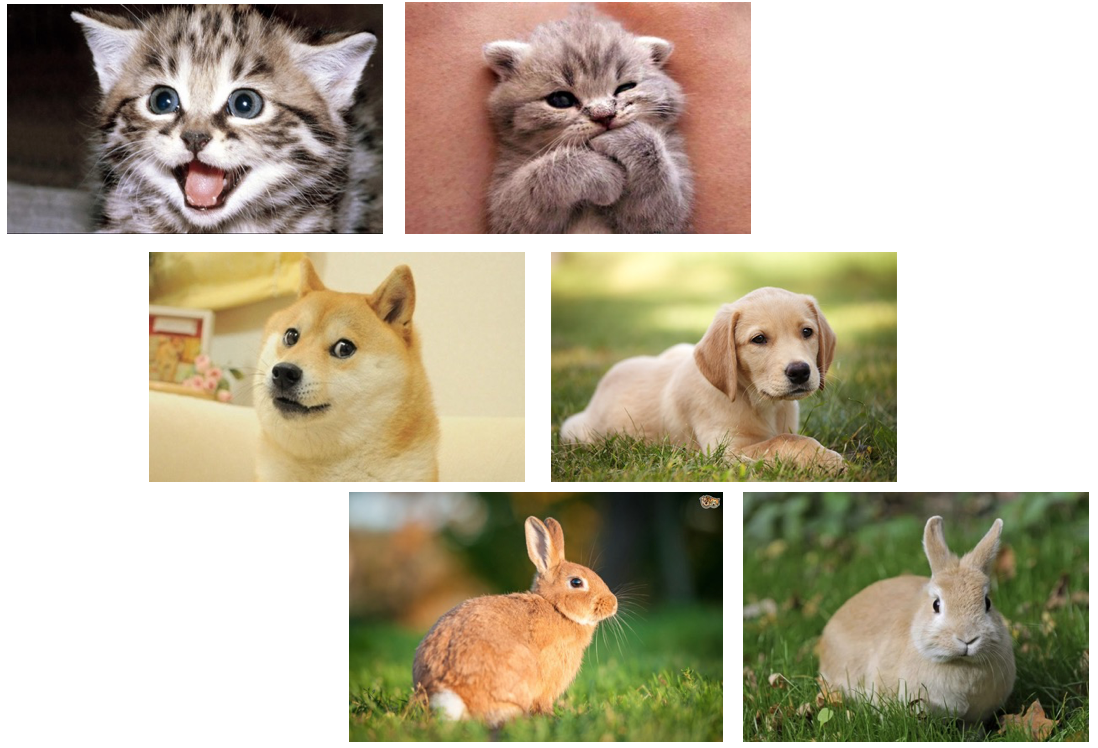
\includegraphics[width=.4\textwidth, height=.2\textheight]{figures/cat-dog-1.png}
	\end{center}
\end{figure}

\break

First of all, we introduce how an image is represented on computer. Mathematically, {gray-scale image can be considered as a matrix  in $ \mathbb{R}^{n_0\times n_0}$ shown below, where the left one is the image from human vision and the right one is the matrix represented in computer. Each entry in this $ \mathbb{R}^{n_0\times n_0}$ corresponds to the value of a pixel belong to $[0,255]$.
	\begin{center}
		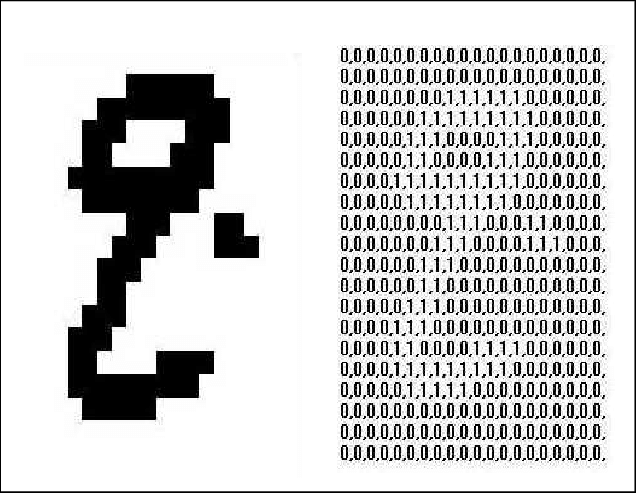
\includegraphics[width=.4\textwidth, height=.2\textheight]{6DL/figures/gray-1.png}
	\end{center}
	
	A color image can be taken as 3D tensor (matrix with $3$ channels (RGB)) in $ \mathbb{R}^{n_0\times n_0 \times 3}$
	\begin{center}
		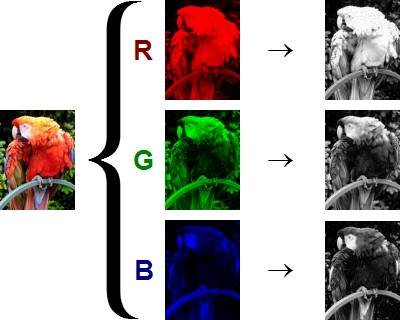
\includegraphics[width=.4\textwidth, height=.2\textheight]{6DL/figures/corlor-1.png}
	\end{center}	
	\break
	
	Then, let us think about the image classification problem of cat, dog and rabbit. Each image is a big vector of pixel values, for example
	$$ d=1280\times720\times 3  (\text{width} \times \text{height} \times \text{RGB channel}) \approx 3\text{M},$$
	which can be considered as a point $x \in \mathbb{R}^d$. The question becomes: given 3 different sets of points (cat, dog and rabbit) in $\mathbb{R}^d$, how does a machine classify them?
	\begin{figure}[H]
		\begin{center}
			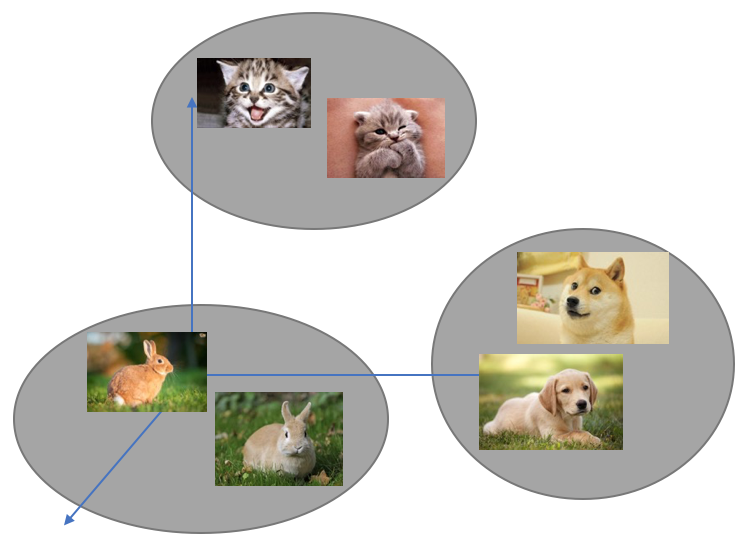
\includegraphics[width=.3\textwidth, height=.3\textwidth]{figures/cat-dog-2.png}   \quad \quad  \quad \quad
			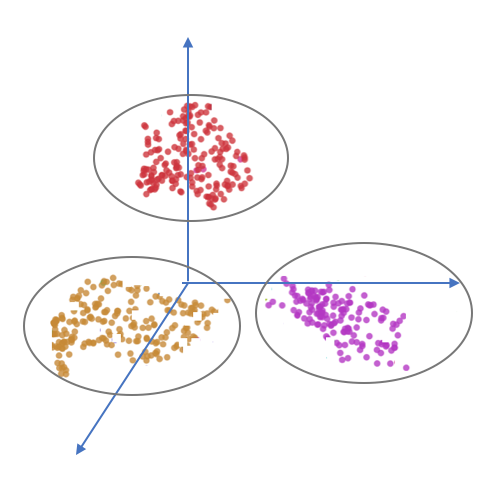
\includegraphics[width=.3\textwidth, height=.3\textwidth]{figures/cat-dog-3.png}
		\end{center}
	\end{figure}
	
	\noindent To answer this question, we consider a mathematical problem: Find $f(\cdot; \bm \theta): \mathbb{R}^d \to \mathbb{R}^3$ such that:
	$$
	f(
\includegraphics[width=.07\textwidth]{figures/cat.png}; \Theta)
	\approx \begin{pmatrix}
	1\\ 0 \\ 0
	\end{pmatrix}
	,\quad
	f(
\includegraphics[width=.07\textwidth]{figures/dog.png}; \Theta)
	\approx \begin{pmatrix}
	0\\ 1 \\ 0
	\end{pmatrix}
	,\quad
	f(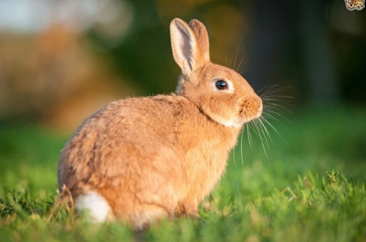
\includegraphics[width=.07\textwidth]{figures/rabbit.png};
	\Theta) \approx
	\begin{pmatrix}
	0\\ 0 \\ 1
	\end{pmatrix}
	.
	$$
	$f(\cdot; \bm \theta)$ maps a given image to a 3-dimensional vector, which is a probability distribution  $\begin{pmatrix}
	p_1\\ p_2 \\ p_3
	\end{pmatrix}$
	, where $p_1, p_2, p_3$ are probabilities of the given image being cat, dog, rabbit, respectively. For example
	
	$$
	f(
\includegraphics[width=.07\textwidth]{figures/cat.png}; \bm \theta)
	=
	\begin{pmatrix}
	0.7\\ 0.2 \\ 0.1
	\end{pmatrix}
	\quad \Longrightarrow \quad 
\includegraphics[width=.07\textwidth]{figures/cat.png}= {\rm cat}.
	$$
	$f$ is a classifier that can be used to classify what a given image is.
	


\break
\section{Some popular data sets in image classification}
In this subsection, we will introduce some popular and standard data sets
in image classification. The most popular four data sets, MNIST, CIFAR-10, CIFAR-100 and ImageNet are shown in Table \ref{popular_dataset}.

\begin{table}[H]
	\centering
	\begin{tabular}{|c|c|c|c|c|c|}
		\hline
		% after \\: \hline or \cline{col1-col2} \cline{col3-col4} ...
		dataset &  training (N) & test (M)   & classes (k) & channels (c)& input size (d)\\\hline
		MNIST	&	60K	&	10K	&	10	& Greyscale & 28*28  \\\hline
		CIFAR-10	&	50K 	&	10K	&	10 & RGB & 32*32   \\\hline
		CIFAR-100	&	50K 	&	10K	&	100 & RGB & 32*32   \\\hline
		ImageNet	&	1.2M 	&	50K	&	1000 &	RGB & 224*224  \\\hline
	\end{tabular}
	\caption{Basic descriptions about popular datasets }
	\label{popular_dataset}
\end{table}

\break
\subsection{MNIST (Modified National Institute of Standards and Technology Database)}
MNIST\cite{lecun1998mnist} is a database for handwritten digits. It is a simple database for people who want to try learning techniques and pattern recognition methods on real-world data while spending minimal efforts on preprocessing and formatting. In order to use MNIST for the classification problem, the following setup is often used:
\begin{itemize}
	\item Training set : $N = 60,000$;
	\item Test set : $M = 10,000$;
	\item Image size : $d =28*28*1=784$;
	\item Classes: $ k = 10$;
\end{itemize}
\begin{figure}[H]
	\begin{center}
		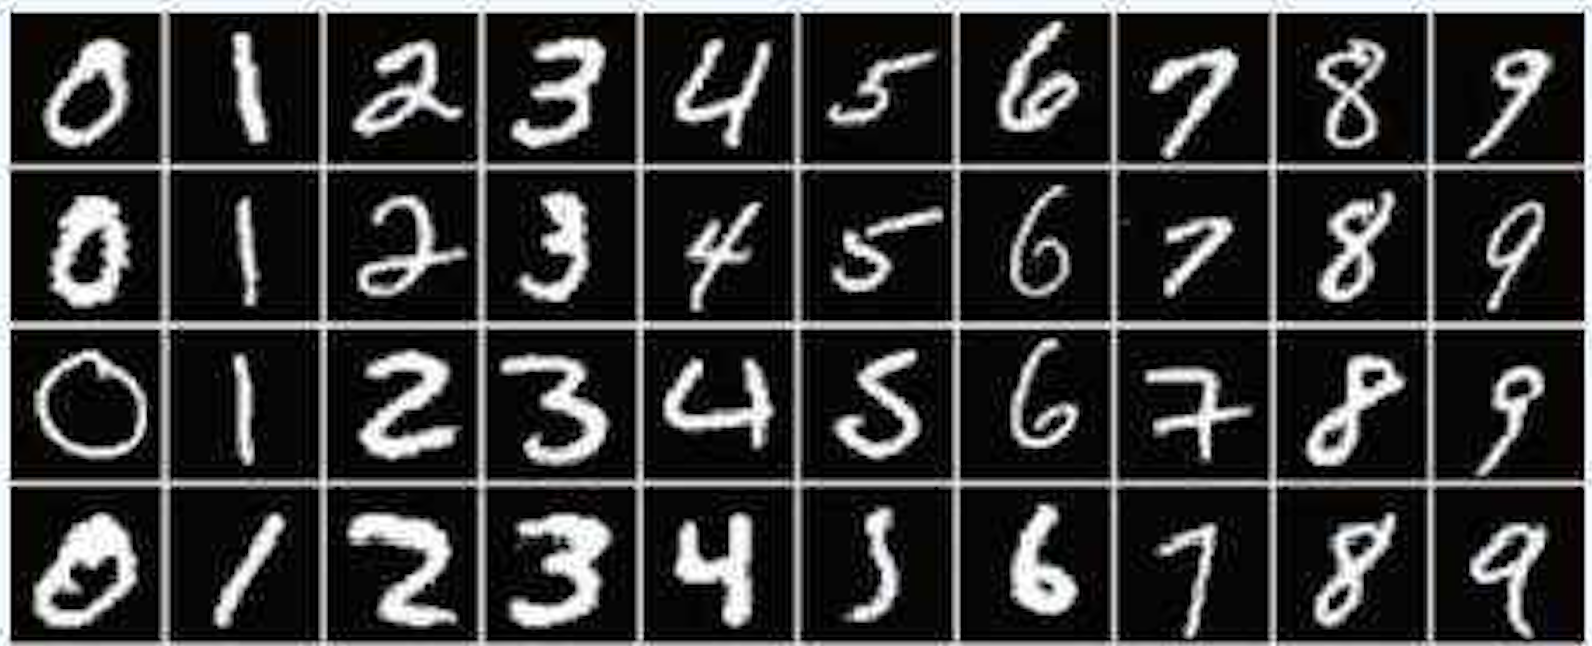
\includegraphics[height=.2\textheight]{mnist_short.png}
		\caption{Some images in MNIST.}
	\end{center}
\end{figure}
The following example shows  an image of handwritten digits is represented mathematically
\break
$$
x=\adjustbox{valign=c}{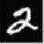
\includegraphics[height=.03\textheight]{mnist2_1.jpg}}
=
\begin{pmatrix}
  x_1\\
x_2\\
\vdots\\
x_{784}
\end{pmatrix}
\in \mathbb R^{784}.
$$
MNIST has 10 classes denoted by $\{A_k\}_{k=1}^{10}$ as shown in the following, where $A_{k}$ is the set of handwritten digits $k$ for $k=1,2,3,...,9$ and $A_{10}$ is the set of handwritten digits $0$
\begin{equation}
  \label{A2}
A_2=
\left\{
\adjustbox{valign=c}{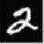
\includegraphics[height=.03\textheight]{mnist2_1.jpg}},
\adjustbox{valign=c}{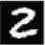
\includegraphics[height=.03\textheight]{mnist2_2.jpg}},\cdots
%\adjustbox{valign=c}{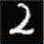
\includegraphics[height=.03\textheight]{mnist2_3.jpg}}, \cdots
\right\},~
%\subset \mathbb R^{784}
A_{9}=
\left\{
\adjustbox{valign=c}{
\includegraphics[height=.03\textheight]{mnist9_1.jpg}},
\adjustbox{valign=c}{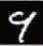
\includegraphics[height=.03\textheight]{mnist9_2.jpg}},\cdots
%\adjustbox{valign=c}{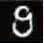
\includegraphics[height=.03\textheight]{mnist9_3.jpg}}, \cdots
\right\},~
A_{10}=
\left\{
\adjustbox{valign=c}{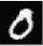
\includegraphics[height=.03\textheight]{mnist0_1.jpg}},
\adjustbox{valign=c}{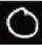
\includegraphics[height=.03\textheight]{mnist0_2.jpg}}, \cdots
%\adjustbox{valign=c}{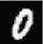
\includegraphics[height=.03\textheight]{mnist0_3.jpg}}, \cdots
\right\}
\subset \mathbb R^{784}.
\end{equation}



\break
\subsection{CIFAR}
\paragraph{CIFAR-10}
CIFAR-10\cite{krizhevsky2009learning} is a set of images that can be used to teach a computer how to recognize objects. It contains 60,000 32x32 color images in 10 different classes,  with 6000 images per class. The 10 different classes represent airplanes, cars, birds, cats, deer, dogs, frogs, horses, ships, and trucks. In order to use CIFAR-10 for the classification problem, people usually use the following setup:
\begin{itemize}
	\item Training set : $N = 50,000$
	\item Test set : $M = 10,000$
	\item Image size : $d  = 32*32*3$
	\item Classes: $k = 10$
\end{itemize}
\begin{figure}[H]
	\begin{center}
		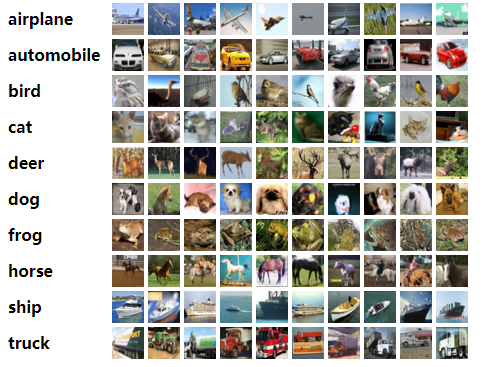
\includegraphics[height=.26\textheight]{cifar10.jpg}
		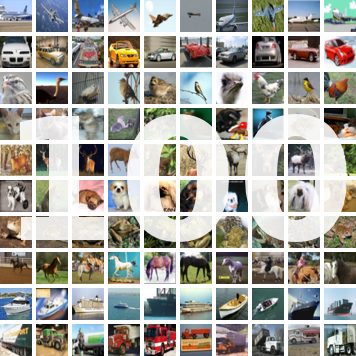
\includegraphics[height=0.26\textheight]{cifar100.png}
		\label{Fig: CIFAR-10}
		\caption{Left: Some images in CIFAR-10. Right: Some images in CIFAR-100.}
	\end{center}
\end{figure}


\break

\paragraph{CIFAR-100}
CIFAR-100\cite{krizhevsky2009learning} is just like the CIFAR-10, except it has 100 classes containing 600 images each. There are 500 training images and 100 testing images per class. The 100 classes in the CIFAR-100 are grouped into 20 superclasses and each superclass has 5 classes. Each image comes with a ``fine" label (the class to which it belongs) and a ``coarse" label (the superclass to which it belongs). In order to use CIFAR-100 for the classification problem, people usually use the following setup:

\begin{itemize}
	\item Training set : $N = 50,000$
	\item Test set : $M = 10,000$
	\item Image size : $d = 32*32*3$
	\item Classes: $k = 100$
	\end{itemize}

\subsection{ImageNet}
The ImageNet\cite{deng2009imagenet} project is a large visual database designed for use in visual object recognition software research. More than 1 million images have been hand labeled to indicate what objects are pictured. It is organized according to the WordNet hierarchy (currently only the nouns), in which each node of the hierarchy is depicted by hundreds and thousands of images.
Since 2010, the ImageNet runs an annual software contest, the ImageNet Large Scale Visual Recognition Challenge (ILSVRC), where software programs compete to correctly classify and detect objects and scenes. In order to use ImageNet for the classification problem, we list the setup of ILSVRC2012 in the following
\begin{itemize}
	\item Training set : $N = 1,200,000$
	\item Test set : $M = 50,000$
	\item Image size : $d = 224*224*3$
	\item Classes: $k = 1,000$
\end{itemize}
\begin{figure}[H]
	\begin{center}
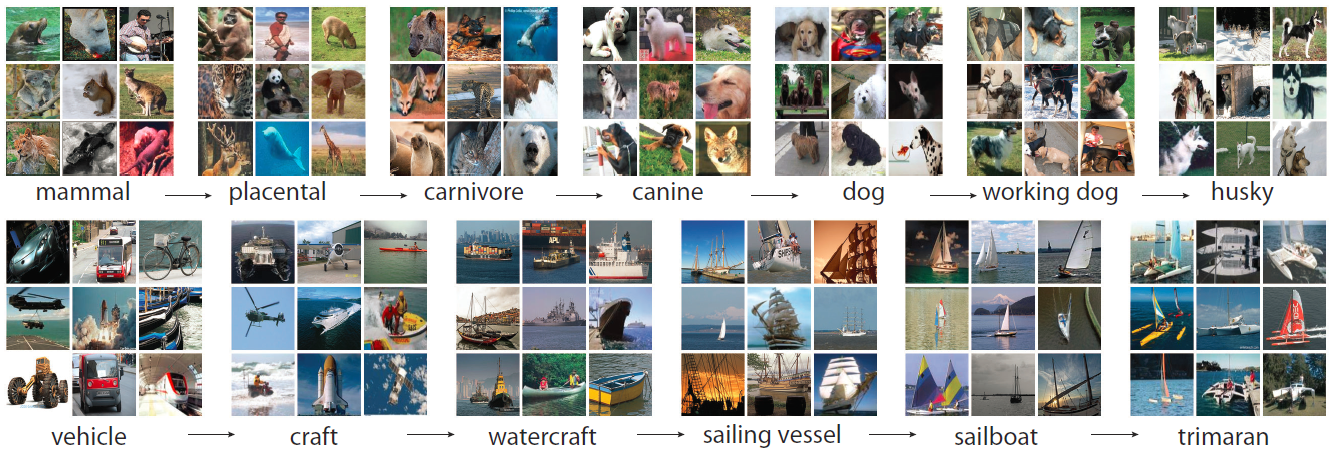
\includegraphics[height=0.22\textheight]{imagenet-example.png}
		\caption{Some images in ImageNet.}
	\end{center}
\end{figure}
\break

\endinput


\chapter{Linear Machine Learning Models} 
%\newpage
In this chapter, we will mainly consider two statistic models, namely
logistic regression for linearly separable sets,
and support vector machine (SVM).
These two linear models form the foundation of deep learning, since
the final fully connected output layer of a deep neural network is
often given by one of these two linear classifiers.  One main objective in this chapter is that  these linear classification models can be used to classify a collection of 
linearly separable classes.  

In the presentation of this chapter, we treat both logistic regression
and support vector machine as pure mathematical techniques for
linearly separable sets.  In the later chapters, we will relate these
techniques in the context of machine learning, especially deep
learning. 
\section{Definition of linearly separable sets}
In this section, we consider a special class of $k$ linearly separable sets for $k\ge 2$.  Let us first introduce the following
definition for binary classification. 


For $k=2$, there is a very simple geometric interpretation of two
linearly separable sets. 
\begin{definition}\label{lem:2class}
  The two sets $A_1$, $A_2\subset \mathbb{R}^d$ are linearly separable
   if there exists a hyperplane
  \begin{equation}
    \label{2classH}
H_0=\{x:wx+b=0\},    
  \end{equation}
 such that $wx+b>0$ if $x\in A_1$ and $wx+b<0$ if $x\in A_2$.
  \end{definition}
\begin{figure}
\centering
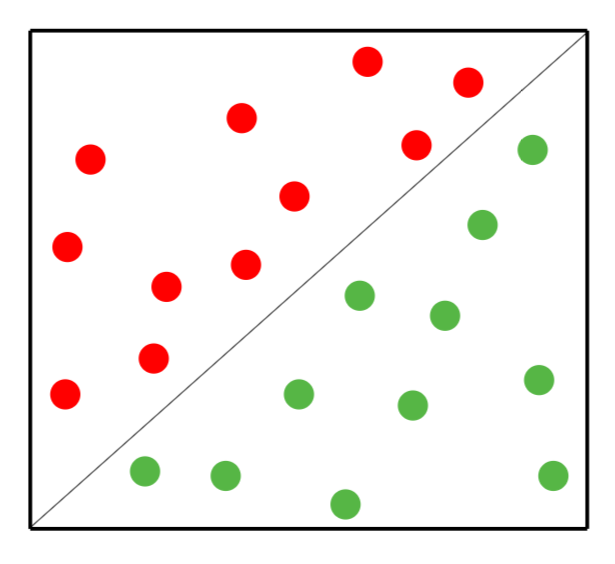
\includegraphics[width=1.5in]{LinearS1.png}  \quad  %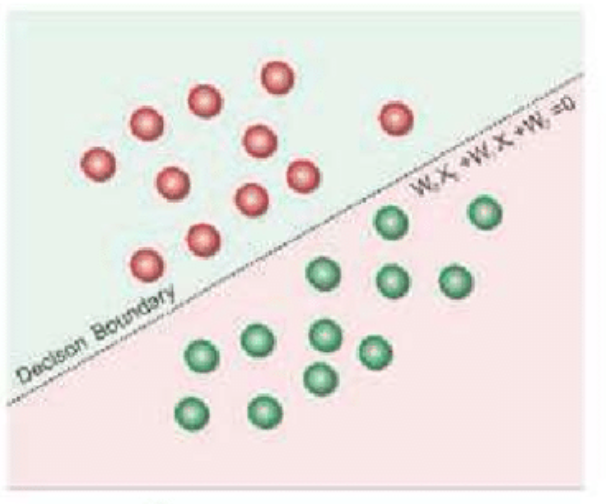
\includegraphics[width=1.5in]{LinearS2.png} 
\caption{One linearly separable set}
\label{twoclassification}
\end{figure}

\begin{figure}
\centering
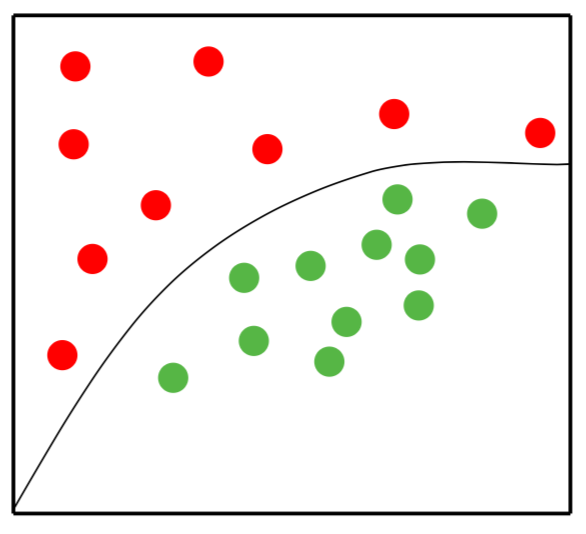
\includegraphics[width=1.5in]{NLinearS1.png}  \quad  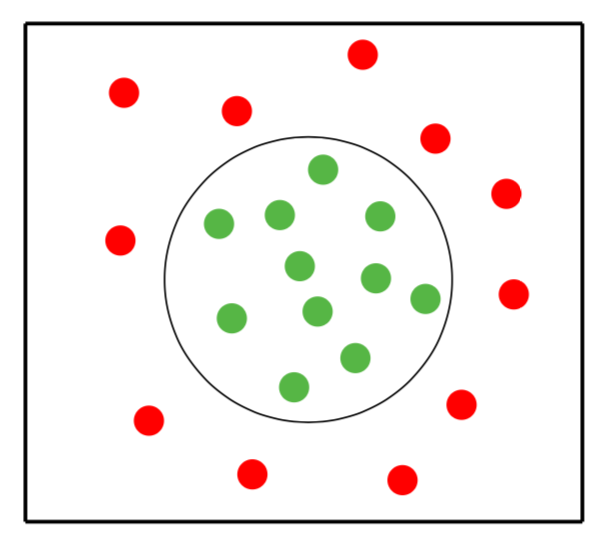
\includegraphics[width=1.5in]{NLinearS2.png} 
\caption{Two non-linearly separable sets}
\label{twoclassification}
\end{figure}

%\blankpage
%\newbreak
\begin{lemma}\label{lem:2class}
  The two sets $A_1$, $A_2\subset \mathbb{R}^d$ are linearly separable
 if there exists 
  \begin{equation}
    \label{Wb}
W=
\begin{pmatrix}
  w_1\\
w_2
\end{pmatrix}
\in \mathbb{R}^{2\times d}, 
b=
\begin{pmatrix}
  b_1\\
b_2
\end{pmatrix}
\in \mathbb{R}^{2\times d}, 
\end{equation}
such that,  % for each $1\le i\le 2$ and $ j \neq i$
\begin{equation}
\label{eq:3}
 w_1x+b_1 > w_2x+b_2,\ \forall x\in A_1,
 \end{equation}
and
\begin{equation}
\label{eq:3}
 w_1x+b_1 < w_2x+b_2,\ \forall x\in A_2.
 \end{equation}
\end{lemma}

\begin{proof}
	Here, we can just take $w = w_1 - w_2$ and $b = b_1 - b_2$, 
	then we can check that the hyperplane $wx + b$ satisfies the
	definition as presented before.
\end{proof}


%\blankpage
%\newbreak
Now let us consider multi-class classification.
To begin with the definition, let us assume that the data space is 
divided into $k$ classes represented by $k$ disjoint sets $A_1,A_2,\cdots,A_k\subset \mathbb{R}^d$, which means
\begin{equation}
A = A_1\cup A_2\cup \cdots \cup A_k, ~A_i\cap A_j = \emptyset, \forall i \neq j.
\end{equation}

\begin{definition}[Linearly Separable]
  A collection of subsets $A_1,...,A_k\subset \mathbb{R}^d$ are
  linearly separable if there exist
  \begin{equation}
    \label{Wb}
W=
\begin{pmatrix}
  w_1\\
\vdots\\
w_k
\end{pmatrix}
\in \mathbb{R}^{k\times d}, 
b=
\begin{pmatrix}
  b_1\\
\vdots\\
b_k
\end{pmatrix}
\in \mathbb{R}^{k\times d}, 
\end{equation}
such that,   for each $1\le i\le k$ and $ j \neq i$
\begin{equation}
\label{eq:3}
 w_ix+b_i > w_jx+b_j,\ \forall x\in A_i.
 \end{equation}
namely, each pairs of $A_i$ and $A_j$ are linearly separable by the plane
\begin{equation}
  \label{Hij}
H_{ij}=\{(w_i-w_j)\cdot x+(b_i-b_j) = 0\}, \quad \forall j\neq i.
\end{equation} 
\end{definition}
The geometric interpretation for linearly separable sets is less
obvious when $k>2$. 
\begin{lemma}{\label{Interplation}}
Assume that $A_1,...,A_k$ are linearly separable and $ W\in
\mathbb{R}^{k\times d} $ and $b\in\mathbb{R}^k $ satisfy \eqref{Wb}.  Define
\begin{equation}
\label{Gammai}
\Gamma_i(W,b) = \{x\in\mathbb R^d: (Wx+b)_i > (Wx+b)_j,\ \forall j \neq i\}     
\end{equation}
Then for each $i$, 
\begin{equation}
  \label{AiGamma}
A_i \subset \Gamma_i(W,b)  
\end{equation}
\end{lemma}
We note that  each $\Gamma_i(W,b)  $ is a polygon whose boundary consists of hyperplanes given by 
\eqref{Hij}.
\begin{figure}
\centering
	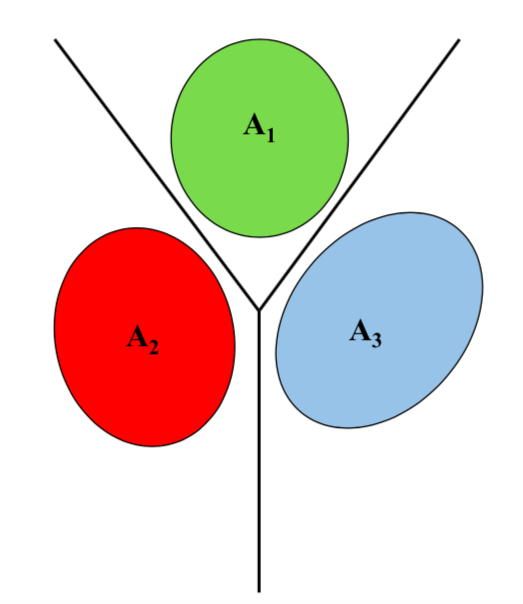
\includegraphics[width=1.5in]{./figures/3-class.PNG}
	\caption{Linearly separable sets in 2-d space (k = 3)}
	\label{twoclassification}
\end{figure}

We next introduce two more definitions of linearly separable sets that
have more clear geometric interpretation. 

\begin{definition}[All-vs-One Linearly Separable]
 A collection of subsets $A_1,...,A_k\subset \mathbb{R}^d$ is
 all-vs-one linearly separable
if for each $i = 1,...,k$, 
$A_i$ and $\displaystyle \cup_{j\neq i} A_j$ are linearly separable. 
\end{definition}

\begin{figure}[H]
\centering
	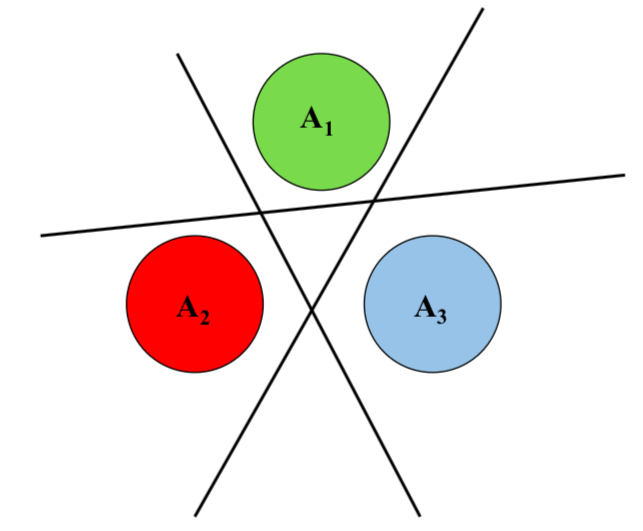
\includegraphics[width=1.5in]{./figures/MulLClassfication.PNG}
	\caption{All-vs-One linearly separable sets (k = 3)}
	\label{twoclassification}
\end{figure}

\begin{definition}[Pairwise Linearly Separable]
  A collection of subsets $A_1,...,A_k\subset \mathbb{R}^d$ is
  pairwise linearly separable if for each pair of indices $1\leq i <
  j\leq k$, 
$A_i$ and $A_j$ are linearly separable. 
\end{definition}



\begin{figure}[H]
\centering
	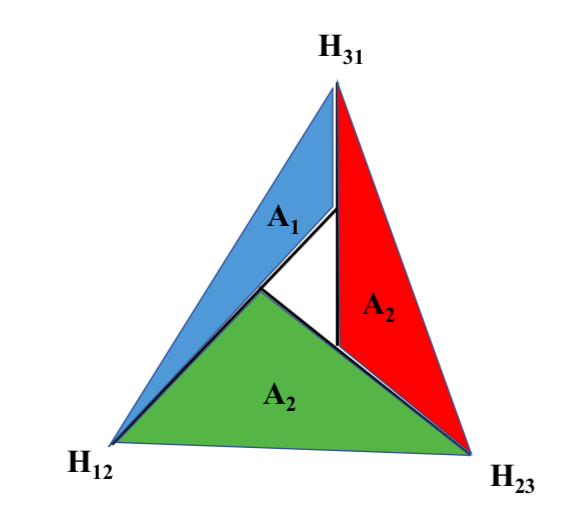
\includegraphics[width=1.5in]{./figures/pairwise_linearly_separable.png}
	\caption{Pairwise linearly separable sets in 2-d space (k = 3)}
	\label{pairwise_separable_example}
\end{figure}


We begin by comparing our notion of linearly separable to the two
other previously introduced geometric definitions of all-vs-one
linearly separable and pairwise lineaerly separable.  Obviously, in
the case of two classes, they are all equivalent, however, with more
than two classes this is no longer the case. We do have the following
implications, though.

\begin{lemma}
  If $A_1,...,A_k\subset \mathbb{R}^d$ are all-vs-one linearly
  separable, then they are linearly separable as well.
\end{lemma}
\begin{proof}
 Assume that $A_1,...,A_k$ are all-vs-one linearly separable. For each $i$, let $w_i$, $b_i$ be such that $w_ix + b_i$ separates
 $A_i$ from $\cup_{j\neq i} A_j$, i.e. $w_ix + b_i > 0$ for $x\in A_i$ and $w_ix + b_i < 0$ for $x \in \cup_{j\neq i} A_j$.
 
 Set $W = (w_1^T,w_2^T,\cdots,w_k^T)^T$, $b = (b_1,b_2,\cdots,b_k)^T$ and observe that if $x\in A_i$, then
 $(Wx + b)_i > 0$ while $(Wx + b)_j < 0$ for all $j\neq i$.
\end{proof}

\begin{lemma}
  If $A_1,...,A_k\subset \mathbb{R}^n$ are linearly separable, then
  they are pairwise linearly separable as well.
\end{lemma}

\begin{proof}
  If $A_1,...,A_k\subset \mathbb{R}^d$ are linearly separable, suppose
  that $W = (w_1^T,w_2^T,\cdots,w_k^T)^T$, $b =
  (b_1,b_2,\cdots,b_k)^T$. So we have
	\begin{equation}
	\begin{cases} 
	w_i x+ b_i > w_j x + b_j & x\in A_i \\
	w_i x+ b_i < w_j x + b_j& x\in A_j \\
	\end{cases}
	\end{equation}
	Take $w_{i,j} = w_i - w_j, b_{i,j} = b_i-b_j$, then we have 
	\begin{equation}
	w_{i,j}x + b_{i,j}\begin{cases} 
	> 0 & x\in A_i \\
	< 0 & x\in A_j \\
	\end{cases}
	\end{equation}
	So $A_1,...,A_k$ are pairwise linearly separable.
\end{proof}

However, the converses of both of these statements are false, as the following examples show.
\begin{example}[Linearly separable but not all-vs-one linearly separable]
 Consider the sets $A_1, A_2, A_3\subset \mathbb{R}$ given by $A_1 = [-4,-2]$, $A_2 = [-1,1]$, and $A_3 = [2,4]$. These
 sets are clearly not one-vs-all linearly separable because $A_2$ cannot be separated from both $A_1$ and $A_3$ by a single
 plane (in $\mathbb{R}$ this is just cutting the real line at a given number, and $A_2$ is in the middle).
 
 However, these sets are linearly separated by $W = [-2,0,2]^T$ and $b = [-3,0,-3]^T$, for example.
\end{example}
\begin{example}[Pairwise linearly separable but not linearly separable]
Consider the sets $A_1, A_2, A_3\subset \mathbb{R}^2$ shown in figure \ref{pairwise_separable_example}.
Note that $A_i$ and $A_j$ are separated by hyperplane $H_{i,j}$ (drawn in the figure) and so these sets are
pairwise linearly separable. We will show that they are not linearly separable.

Assume to the contrary that $W\in \mathbb{R}^{3\times 2}$ and $b\in \mathbb{R}^2$ separate $A_1$, $A_2$, and $A_3$. Then
$(w_i - w_j)x + (b_i - b_j)$ must be a plane which separates $A_i$ and $A_j$. Now consider a point $z$ bounded by $A_1$, $A_2$ and $A_3$ in figure 
\ref{pairwise_separable_example}. We see from the figure that given any plane separating $A_1$ from $A_2$, $z$ must
be on the same side as $A_2$, given any plane separating $A_2$ from $A_3$, $z$ must be on the same side as
$A_3$, and given any plane separating $A_3$ from $A_1$, $z$ must be on the same side as $A_1$.

This means that $(w_2 - w_1)z + (b_2 - b_1) > 0$, $(w_3 - w_2)z + (b_3 - b_2) > 0$, and
$(w_1 - w_3)z + (b_1 - b_3) > 0$. Adding these together, we obtain $0 > 0$, a contradiction.

The essence behind this example is that although the sets $A_1$, $A_2$, and $A_3$ are pairwise linearly separable, 
no possible pairwise separation allows us to consistently classify arbitrary new points. However, a linear separation
would give us a consistent scheme for classifying new points.

\end{example}

So the notion of linear separability is sandwiched in between the more
intuitive notions of all-vs-one and pairwise separability. It turns
out that linear separability is the notion which is most useful for
the $k$-class classification problem and so we focus on this notion of
separability from now on.




\newpage
\section{Some simple linear classifiers}
We begin with the simplest situation, where there are only two classes.
\begin{lemma}
If $A_1$, $A_2\subset\mathbb{R}^n$ are linearly separable, then there exists $w\in\mathbb{R}^{1\times n}$, $b\in\mathbb{R}$ such that
        \begin{equation}
          f(x):=h\left( \begin{array}{cc}
              wx+b \\
              -(wx+b)
            \end{array}
          \right)
          =
          \begin{cases}
            e_1 \quad x\in A_1 \\
            e_2 \quad x\in A_2,
          \end{cases}
        \end{equation}
      where $e_1=\left( \begin{array}{cc} 1\\0 \end{array} \right)$,
      $e_2=\left( \begin{array}{cc} 0\\1 \end{array} \right)$ and
        $h$ is the Heaviside function defined by:
        \begin{equation}
        \label{heaviside}
        h(t):=\begin{cases}
        0 \quad t < 0, \\
        1 \quad t \ge 0 .
        \end{cases}
        \end{equation}
      \end{lemma}
      The Heaviside function $h$ defined in \eqref{heaviside} is a
      classic activation function. 
      \begin{figure}
      	\centering
      	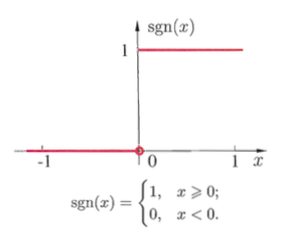
\includegraphics[width=2in]{figures/Heaviside.png}   
      	\caption{Heaviside activation function }
      \end{figure}
      
      But its discontinuity at $t=0$
      makes it difficult to use in practice. Instead we consider the
      following linear-step function:
  \begin{equation}\label{linear-step}
  \sigma(t)=
    \begin{cases}
       0 \quad t<0, \\
      t\quad 0\le t\le 1, \\
     1 \quad t> 1. \\
    \end{cases}
  \end{equation}
\begin{figure}
\centering
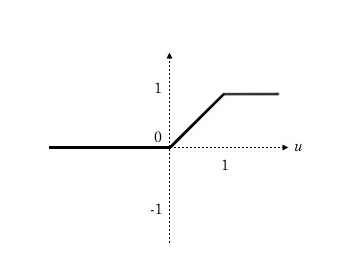
\includegraphics[width=2in]{./figures/zig}   
\caption{Linear-step function}
\end{figure}
This $\sigma(t)$ is closely related to the so-called Rectified Linear Unit function: 
\begin{equation}\label{ReLU}
ReLU(t):=\begin{cases}
0 \quad t< 0, \\
t \quad t\ge 0. 
\end{cases}
\end{equation}
\begin{figure}
\centering
\includegraphics[width=2in]{./figures/ReLU}   
\caption{ReLU activation function }
\end{figure}
Namely 
\begin{equation}
  \label{sigma-ReLU}
\sigma(t)=ReLU(t)-ReLU(t-1).
\end{equation}

\begin{lemma}
	If $A_1$, $A_2\subset\mathbb{R}^n$ are linearly separable, then there exist $w\in\mathbb{R}^{1\times n}$, $b\in\mathbb{R}$ such that
	\begin{equation}
	f(x):=\left( \begin{array}{cc}
	\sigma(wx+b) \\
	\sigma(-(wx+b))
	\end{array}
	\right)
	= e_i,\quad\mathrm{if}\ x\in A_i,\ i=1,2.
	\end{equation}
\end{lemma}
\begin{proof}
  By the definition of linearly separable sets, there exist
  $w_0\in\mathbb{R}^{1\times n}$, $b_0\in\mathbb{R}$ such that
  $w_0x+b_0>0$ if $x\in A_1$ and $w_0x+b_0<0$ if $x\in A_2$. We can
  find $\varepsilon>0$ such that
\begin{equation}
w_0x+b_0\begin{cases}
>\varepsilon \qquad x\in A_1, \\
<-\varepsilon \quad x\in A_2 .
\end{cases}
\end{equation}
Let $w=w_0/\varepsilon$, $b=b_0/\varepsilon$, we have:
\begin{equation}
wx+b\begin{cases}
>1 \qquad x\in A_1, \\
<-1 \quad x\in A_2 .
\end{cases}
\end{equation}
which implies $f(x)=e_i$ if $x\in A_i$.
\end{proof}

The extension of the above lemma to $k$-classes is straightforward.
\begin{lemma}
  If $A_i \subset \mathbb{R}^n(1\le i \le k)$ are linearly separable,
  there exist $W\in\mathbb{R}^{k\times n}$, $b\in\mathbb{R}^k$ s.t.
\begin{equation}
  \label{simple-f}
	f(x):=\sigma(Wx+b) = e_i,\quad\mathrm{for\ }x\in A_i  
\end{equation}
\end{lemma}

Oftentimes, we use the following notation
\begin{equation}
  \label{theta}
\theta=(W,b)\in\mathbb{R}^{k\times(n+1)} \mbox{ and } \theta[x]=Wx+b.
\end{equation}

\newpage  
\section{Introduction to logistic regression}
In this section, we introduce techniques related to basic logistic regression, see \cite{gelman2006data} for more details.
\subsection{Logistic regression}\label{sec:LR}
%We first introduce the next definition of the set of linearly classifiable weights.

Assume that we are given $k$ linearly separable sets $A_1,A_2,\cdots,A_k\in \mathbb{R}^d$, we define the set of classifiable weights as
	\begin{equation}
	\bm\Theta = \{\bm\theta = (W,b): w_ix+b_i>w_jx+b_j,~\forall x\in A_i, j\neq i, i= 1,\cdots,k\}
	\end{equation}
	which means those $(W,b)$ can separate $A_1,A_2,\cdots,A_k$ correctly. 
	

Our linearly separable assumption implies that $\bm\Theta\neq \emptyset$. 
Now we know the existence of linearly classifiable weights. But how can we find one element in $\bm\Theta$?

\begin{definition}[soft-max]\label{softmax}
 Given $s = (s_1,s_2,\cdots,s_k)^T\in \mathbb{R}^k$, we define the soft-max mapping $\sigma: \mathbb{R}^k \rightarrow\mathbb{R}^k $ as
 \begin{equation}
 \sigma(s)  = \frac{e^{s}}{e^{s}\cdot \bm{1}} = \frac{1}{\sum\limits_{i=1}^k e^{s_i}}
 \begin{pmatrix}
 e^{s_1}\\
 e^{s_2}\\
 \vdots\\
 e^{s_k}
 \end{pmatrix}
 \end{equation}
 where $e^{s} = 
 \begin{pmatrix}
 e^{s_1}\\
 e^{s_2}\\
 \vdots\\
 e^{s_k}
 \end{pmatrix}
 $, $\bm{1} = 
 \begin{pmatrix}
 1\\
 1 \\
 \vdots \\
 1
 \end{pmatrix} \in\mathbb{R}^k$.
\end{definition}


\begin{definition}
 Given parameter $\bm\theta = (W,b)$, we define a feature mapping $\bm p: \mathbb{R}^d \rightarrow \mathbb{R}^k$ as
 \begin{equation}
 \bm p(x; \bm\theta)  = \sigma(Wx+b) = \frac{1}{\sum\limits_{i=1}^k e^{w_i x+b_i}}
 \begin{pmatrix}
 e^{w_1 x+b_1}\\
 e^{w_2 x+b_2}\\
 \vdots\\
 e^{w_k x+b_k}
 \end{pmatrix}
 = \begin{pmatrix}
 p_1(x; \bm\theta) \\
 p_2(x; \bm\theta) \\
 \vdots \\
 p_k(x; \bm\theta)
 \end{pmatrix}
 \end{equation}
 where the $i$-th component 
 \begin{equation}\label{key}
 p_i(x; \bm\theta) = \frac{e^{w_i x+b_i}}{\sum\limits_{i=1}^k e^{w_i x+b_i}}.
 \end{equation}
\end{definition}



The soft-max mapping have several important properties.
\begin{enumerate}
	\item 
	$\displaystyle 0< p_i(x; \bm\theta) <1,~\sum_i p_i(x; \bm\theta) = 1$. 
	
	This implies that $\bm p(x; \bm\theta)$ can be regarded as a probability distribution of data points which means that given $x\in \mathbb{R}^d$, we have $x\in A_i$ with probability $p_i(x; \bm{\theta})$, $i = 1,\cdots,k$. 
	\item 
	$p_i(x; \bm\theta)>p_j(x; \bm\theta)\Leftrightarrow w_ix+b_i>w_j x+b_j.$
	
	This implies that the linearly classifiable weights have an equivalent description as
	\begin{equation}
	\bm{\Theta} = \left\{\bm\theta: p_i(x; \bm\theta)>p_j(x; \bm\theta),~\forall x\in A_i, j\neq i, i= 1,\cdots,k\right\}
	\end{equation}
	\item We usually use the max-out method to do classification. For a given data point $x$, we first use a soft-max mapping to map it to $\bm p(x; \bm\theta)$, then we attach $x$ to the class $i= \arg\max_j p_i(x; \bm\theta)$. 
	
	This means that we pick the label $i$ as the class of $x$ such that $x\in A_i$ has the biggest probability $p_i(x; \bm\theta)$.
\end{enumerate}
More detailed discussion of logistic regression from the probability perspective will be presented in the nearly future. 

From the above properties, we can define the following likelihood function to help find elements in $\bm{\Theta}$:
\begin{equation}
P (\bm\theta)=
\prod\limits_{i = 1}^k \prod\limits_{x\in A_i} p_i(x; \bm\theta).
\end{equation} 
%The next lemma shows that we can use this function to help us find some linearly classifiable weights.
%\begin{theorem}\label{thm1-H}
%	If $ \bm \theta \notin \Theta$, then there exists $ \bm \theta^* \in\bm \Theta$ such that 
%	\begin{equation}\label{key}
%	H( \bm \theta^*) > H(\bm \theta).
%	\end{equation}
%\end{theorem}
Based on the property that
\begin{equation}\label{key}
p_i (x; \bm \theta) = \max_{1\le j \le k} p_j(x; \bm \theta), \quad\forall x \in A_i,\ \bm \theta \in \Theta,
\end{equation}
we may use the next optimization problem
\begin{equation}\label{key}
\max_{\bm \theta\in \bm{\Theta}} P(\bm \theta).
\end{equation}
to find an element in $\bm{\Theta}$. 
More precisely, let us introduce the next lemmas (properties) of $P(\bm \theta)$.
\begin{lemma}\label{lemm:H1/2}
	Assume that the sets $A_1,A_2,\cdots,A_k$ are linearly separable. Then we have
	\begin{equation}
	\left\{\bm \theta:~P(\bm\theta)>\frac{1}{2}\right\}\subset \bm{\Theta}.
	\end{equation}
\end{lemma}
\begin{proof}
	It suffices to show that if $\bm\theta \not\in \bm\Theta$, we must have $P(\bm\theta)\leq\frac{1}{2}$.
	For any $\bm\theta \not\in
	\bm\Theta$, there must exist an $i_0$ ,an $x_0\in A_{i_0}$ and a
	$j_0\neq i_0$ such that
	\begin{equation}
	w_{i_0} x_0 + b_{i_0} \leq w_{j_0}x_0 + b_{j_0}.
	\end{equation}
	Then we have
	\begin{equation}
	p_{i_0}(x_0; \bm\theta) \leq \frac{e^{w_{i_0} x_0 + b_{i_0}}}{e^{w_{i_0} x_0+b_{i_0}}+e^{w_{j_0} x_0+b_{j_0}}} \leq\frac{1}{2}.
	\end{equation}
	Notice that $p_i(x; \bm \theta) < 1$ for all $i = 1,\cdots,k$, $x\in A$.
	So
	\begin{equation}
	P(\bm\theta) <  p_{i_0}(x_0; \bm\theta) \leq \frac{1}{2}.
	\end{equation}
\end{proof}

\begin{lemma}
	If $A_1,A_2,\cdots,A_k$ are linearly separable and $\bm\theta \in \bm\Theta$, we have
	\begin{equation}
	\lim_{\alpha\rightarrow +\infty}p_i(x; \alpha\bm\theta) = 1\Leftrightarrow x\in A_i. 
	\end{equation}
\end{lemma}
\begin{proof}
	We first note that if  $x\in A_i$,
	\begin{equation}
	 p_i(x,\bm \theta) = \frac{1}{1+\sum\limits_{j\neq i}e^{\alpha[(w_j x+ b_j)-(w_i x+b_i)]}} \to 1, \quad \text{as} \quad \alpha \to \infty.
	\end{equation}
	On the other hand, if $x\not\in A_i$, 
	\begin{equation}
	p_i(x; \bm\alpha\bm\theta) = \frac{1}{1+\sum\limits_{j\neq i}e^{\alpha[(w_j x+ b_j)-(w_i x+b_i)]}} \leq \frac{1}{2}.
	\end{equation}
	This implies that if $x\not\in A_i$, $\lim_{\alpha\rightarrow \infty}p_i(x; \alpha\bm \theta)\neq 1$ which is equivalent to the proposition that if $\lim_{\alpha\rightarrow \infty}p_i(x; \alpha\bm \theta)= 1$, then $x\in A_i$.
\end{proof}

\begin{lemma}{\label{thm2}} If $A_1,A_2,\cdots,A_k$ are linearly separable, 
	\begin{equation}
	\bm\Theta = \left\{\bm\theta: \lim_{\alpha\rightarrow +\infty}P(\alpha\bm\theta) = 1\right\}.
	\end{equation}
\end{lemma}

\begin{proof}
 	We first note that if $\bm\theta \in\bm\Theta$, we have $\displaystyle\lim_{\alpha\rightarrow +\infty}p_i(x; \alpha\bm\theta) = 1$ for all $x\in A_i$. So
	\begin{equation}
	\lim\limits_{\alpha\rightarrow +\infty} P(\alpha\bm\theta) = \lim\limits_{\alpha\rightarrow +\infty} \prod\limits_{i = 1}^k \prod\limits_{x\in A_i} p_i(x; \alpha\bm\theta) = \prod\limits_{i = 1}^k \prod\limits_{x\in A_i} \lim\limits_{\alpha\rightarrow +\infty}p_i(x; \alpha\bm\theta) = 1.
	\end{equation}
	On the other hand, if $\lim\limits_{\alpha\rightarrow +\infty} P(\alpha\bm\theta) = 1$, there must exist one $\alpha_0>0$ such that $P(\alpha_0\bm\theta) >\frac{1}{2}$. From Lemma~\ref{lemm:H1/2}, we have $\alpha_0\bm\theta\in\bm\Theta$, which means $\bm\theta\in\bm\Theta$.
\end{proof}


These properties above imply that if we can obtain a classifiable weight through maximizing $P(\bm\theta)$, while lemma \ref{thm2} tells us that $P(\bm\theta)$ will not have a global minimum actually.

More specifically, we just need to find some $\bm \theta \in \Theta$ such that
\begin{equation}\label{key}
P(\bm \theta) > \frac{1}{2} \Leftrightarrow  L(\bm \theta) : = -\log P(\bm \theta )  < \log(2).
\end{equation}
%{\bf Question:} how to find these element?

\blankpage
\break
\subsection{Regularized logistic regression}
Here, we start from the regularization term $e^{-\lambda R(\|\bm\theta\|)}$ with 
these next properties:
\begin{enumerate}
	\item $\lambda > 0$.
	\item $R(t)$ is a strictly increasing function on $\mathbb{R}^+$ with $R(0) = 0$, $\lim\limits_{t\rightarrow +\infty} R(t) = +\infty$.
	For example, $R(t) = t^2$.
	\item $\|\cdot\|$ is a norm on $R^{k\times(d+1)}$, a commonly used norm  is the 
	following Frobenius norm: 
	\begin{equation}\label{key}
	\|\bm \theta\|_F = \sqrt{\sum_{i,j}W_{ij}^2 + \sum_i b_i^2}.
	\end{equation}
\end{enumerate}

Based on this regularization term,  we may consider the following 
regularized likelihood function $P_\lambda(\bm\theta)$ as 
\begin{equation}\label{key}
 P_\lambda(\bm\theta) = P(\bm\theta)e^{-\lambda R(\|\bm\theta\|)}.
\end{equation}


Here, let us define 
\begin{equation}\label{key}
\bm\Theta_{\lambda} = \mathop{{\arg\max}}_{\bm\theta}  P_\lambda(\bm\theta),
\end{equation}
where 
\begin{equation}\label{key}
\mathop{\arg\max}_{\bm\theta}  P_\lambda(\bm\theta) = \left\{\bm \theta ~:~ P_\lambda(\bm \theta) = \max_{\bm \theta} P_\lambda(\bm \theta) \right\}.
\end{equation}


The next lemma show that the maximal set of modified objective is not empty.
\begin{lemma}Suppose that $A_1,A_2, \cdots, A_k$ are linearly separable, then
	\begin{enumerate}
		\item if $\lambda = 0$, $\bm\Theta_0 = \emptyset$,
		\item $\bm\Theta_{\lambda}$ must be nonempty for all $\lambda>0$.
	\end{enumerate}
\end{lemma}
\begin{proof}
	Lemma~\ref{thm2} shows the first proposition. For the second proposition, 
	we notice that 
	\begin{enumerate}
		\item $ P_\lambda(\bm 0) = \frac{1}{k^N}$.
		\item $\exists\ M_{\lambda}>0$ such that $e^{-\lambda R(\|\bm\theta\|)}<\frac{1}{k^N}$ whenever $\|\bm\theta\|> M_{\lambda}$ because of the properties of $R(\|\bm\theta\|)$.
	\end{enumerate}
	So a maxima on $\{\bm\theta: \|\bm\theta\| \le M_{\lambda}\}$ must be a global maxima. Then we can easily obtain the result in the lemma from the boundedness and closeness of $\{\bm\theta: \|\bm\theta\| \le M_{\lambda}\}$.
\end{proof}

Furthermore, we have the next theorem which shows that we can indeed get $\Theta$ by maximizing $P_\lambda(\bm \theta)$.
\begin{theorem}\label{thm-L-Theta} If $A_1,A_2,\cdots,A_k$ are linearly separable, 
	\begin{equation}\label{key}
	\bm\Theta_{\lambda} \subset \bm\Theta,
	\end{equation}
when $\lambda>0$ and sufficiently small.
\end{theorem}
\begin{proof}
By Lemma~\ref{lemm:H1/2}, we can take $\bm\theta_0\in \bm\Theta$ such that $P(\bm\theta_0)> \frac{3}{4}$.
Then, for any $\lambda < \frac{\log \frac{3}{2}}{R(\|\bm\theta_0\|)}$, $\bm\theta_{\lambda}\in \bm\Theta_{\lambda}$, we have
		\[
		P(\bm\theta_{\lambda}) \geq  P_\lambda(\bm\theta_{\lambda})  \geq P_\lambda(\bm \theta_0) = P(\bm\theta_0)e^{-\lambda R(\|\bm\theta_0\|)} > \frac{3}{4}\cdot \frac{2}{3} = \frac{1}{2},
		\]
		which implies that $\bm \theta_{\lambda} \in \Theta$.
		Thus, for any $ 0< \lambda < \frac{\log \frac{3}{2}}{R(\|\bm\theta_0\|)}$, $\bm\Theta_{\lambda} \subset \bm\Theta$.

\end{proof}


The design of logistic regression is that 
maximize $P_\lambda(\bm\theta)$ is equivalent to minimize $-\log P_\lambda(\bm\theta)$, i.e.,
\begin{equation}\label{key}
\max_{\bm \theta} \left\{ P_\lambda(\bm\theta) \right\} \Leftrightarrow \min_{\bm \theta} \left\{ -\log   P_\lambda(\bm\theta)\right\},
\end{equation}
while the second one is more convenient to evaluate the gradient. Meanwhile, we add a regularization term $R(\bm\theta)$ to the objective function which makes the optimization problem has a unique solution. 

 Mathematically, we can formulate Logistic regression as
\begin{equation}
\min_{\bm\theta} L_\lambda(\bm \theta),
\end{equation}
where
\begin{equation}\label{eq:logisticlambda}
L_\lambda(\bm \theta)  := -\log P_\lambda(\bm\theta) = -\log P(\bm\theta) + \lambda R(\|\bm\theta\|) = L(\bm\theta) + \lambda R(\|\bm\theta\|),
\end{equation}
with
\begin{equation}\label{logistic}
L(\bm \theta) = - \sum_{i=1}^k \sum_{x\in A_i} \log p_{i}(x;\bm \theta).
\end{equation}



Then we have the next logistic regression algorithm.
\begin{algorithm}[H]
	\caption{Logistic Regression} 
	\label{alg:LR-R}
	Given data $A_1, A_2, \cdots, A_k$, find 
	\begin{equation}\label{key}
	\bm \theta^* = \mathop{\arg\min}_{\bm \theta}  L_\lambda(\bm \theta),
	\end{equation}
	for some sufficient small $\lambda > 0$.
\end{algorithm}

\begin{remark}
	Here
	\begin{equation}\label{key}
	L(\bm \theta)  = -\log P(\bm\theta),
	\end{equation}
	is known as the loss function of logistic regression model.
	The next reasons may show that why $L(\bm \theta)$ is popular.
	\begin{enumerate}
		\item It is more convenient to take gradient for $L(\bm \theta)$ than $P(\bm \theta)$.
		\item $L(\bm \theta)$ is related the so-called cross-entropy 
		loss function which will be discussed in the next section.
		\item $L(\bm \theta)$ is a convex function which will be discussed later.
	\end{enumerate}
\end{remark}



\endinput
\begin{lemma}
	If $A_1,A_2,\cdots,A_k$ are linearly separable, $-\log H(\bm\theta)$ has no global minimum.
\end{lemma}

\begin{theorem}
	$-\log P(\bm\theta) + \lambda R(\bm\theta)$ has a global minimizer for sufficiently small $\lambda>0$. 
\end{theorem}


Denote the above objective function as
\begin{equation}
L(\theta,\alpha) = \alpha (\max_i \|w_i\|_2) + \displaystyle\sum_{i=1}^k \displaystyle\sum_{x\in A_i} 
\left(\log(\mathbbm{1}^T\exp(W x + b)) - (W x + b)_i\right)
\end{equation}
where $\theta = (W,b)$. And we denote a linear separable parameter set $\Theta$ as
\begin{equation}
\Theta = \{\theta~|w_ix + b_i > w_jx + b_j, x\in A_i,~j\neq i\}
\end{equation}
Set
\begin{equation}
p_i(\theta,x) = \frac{e^{w_i x+b_i}}{\sum\limits_{j=1}^k e^{w_j x+b_j}},   \forall i = 1,\cdots,k.
\end{equation}
and define the LR classifiable parameter set $\bar{\Theta}$ as
\begin{equation}
\bar{\Theta} = \{\theta~|p_i(\theta,x)>p_j(\theta,x), ~x\in A_i,~j\neq i\}
\end{equation}
Easy to observe that 
\begin{equation}
\Theta = \bar{\Theta}
\end{equation}




\begin{theorem}
	Assume that $R(\theta)\geq 0$ is an non-negative function such that 
	\begin{equation}
	\Theta^*(\lambda)={\rm argmax}\ P(\theta)e^{-\lambda R(\theta)} \neq \emptyset, \quad \forall \lambda>0
	\end{equation}
	then for sufficiently small $\lambda>0$, 
	$$ \Theta^*(\lambda)\subset \left\{ \theta: P(\theta)\geq \frac{1}{2} \right\}\subset \Theta.$$
\end{theorem}

\begin{proof}
	Given $\theta_0\in\Theta$. Let $\alpha >0$ be such that 
	$$P(\alpha \theta_0)\geq \frac{2}{3}$$
	Let $\lambda>0$ be sufficiently small such that 
	$$e^{-\lambda R(\theta)}>\frac{3}{4}$$
	For any $\theta \in \Theta^*$  
	$$
	P(\theta)e^{-\lambda R(\theta)} \geq P(\alpha \theta_0) e^{-\lambda R(\alpha\theta_0)} > \frac{2}{3}\cdot \frac{3}{4}=\frac{1}{2}$$
	Then $P(\theta)>\frac{1}{2}$.
\end{proof}  

%\newbreak
\section{KL divergence and cross-entropy}
Cross-entropy minimization is frequently used in optimization and rare-event probability estimation. When comparing a distribution    against a fixed reference distribution, cross-entropy and KL divergence are identical up to an additive constant. See more details in \cite{murphy2012machine,kullback1951information,kullback1997information} and the reference therein.

The KL(Kullback--Leibler) divergence defines a special distance between two discrete probability distributions 
$$
p=\left( \begin{array}{ccc}
p_1\\
\vdots \\
p_k
\end{array} \right),\quad  q=\left( \begin{array}{ccc}
q_1\\
\vdots \\
q_k
\end{array} \right)
$$
with $0\le p_i, q_i\le1$ and $\sum_{i=1}^{k}p_i=\sum_{i=1}^{k}q_i=1$ by
\begin{equation}
\label{KL-divergence}
D_{\rm KL}(q,p)= \sum_{i=1}^k q_i\log \frac{q_i}{p_i}.  
\end{equation}

\begin{lemma}\mbox{}
$D_{\rm KL}(q,p)$ works like a ``distance" without the symmetry:
	\begin{enumerate}
		\item $D_{\rm KL}(q,p)\ge0$;		
		\item $D_{\rm KL}(q,p)=0$ if and only if $p=q$;
	\end{enumerate}
\end{lemma}

\begin{proof}We first note that the elementary inequality
	\begin{equation}
	\log x \le x - 1, \quad\mathrm{for\ any\ }x\ge0,
	\end{equation}
	and the equality holds if and only if $x=1$.
	\begin{equation}
	-D_{\rm KL}(q,p) = - \sum_{i=1}^c q_i\log \frac{q_i}{p_i}   = \sum_{i=1}^k q_i\log \frac{p_i}{q_i} \le \sum_{i=1}^k q_i( \frac{p_i}{q_i}  - 1) = 0.
	\end{equation}
	And the equality holds if and only if 
	\begin{equation}
	\frac{p_i}{q_i} = 1 \quad \forall i = 1:k.
	\end{equation}
\end{proof}

Define cross-entropy for distribution $p$ and $q$ by
\begin{equation}\label{Cross-Entropy}
H(q,p) = - \sum_{i=1}^k q_i \log p_i,
\end{equation}
and the entropy for distribution $q$ by 
\begin{equation}\label{Entropy}
H(q) = - \sum_{i=1}^k q_i \log q_i.
\end{equation}
Note that
\begin{equation}
D_{\rm KL}(q,p)= \sum_{i=1}^k q_i\log \frac{q_i}{p_i} =  \sum_{i=1}^k q_i \log q_i - \sum_{i=1}^k q_i \log p_i
\end{equation}
Thus, 
\begin{equation}\label{KLandEntropy}
H(q,p) = H(q) + D_{\rm KL}(q,p).
\end{equation} 
It follows from the relation \eqref{KLandEntropy} that
\begin{equation}
\label{EntropyandKL}
\mathop{\arg\min}_p D_{\rm KL}(q,p)=\mathop{\arg\min}_p H(q,p).
\end{equation}

The concept of cross-entropy  can be used to define a loss function in machine learning and optimization. 
Let us assume $y_i$ is the true label for $x_i$, for example $y_i = e_{k_i}$ if $x_i \in A_{k_i}$. Consider the predicted distribution 
\begin{equation}\label{key}
\bm p(x; \bm \theta) = \frac{1}{\sum\limits_{i=1}^k e^{w_i x+b_i}}
\begin{pmatrix}
e^{w_1 x+b_1}\\
e^{w_2 x+b_2}\\
\vdots\\
e^{w_k x+b_k}
\end{pmatrix}
= \begin{pmatrix}
p_1(x; \bm\theta) \\
p_2(x; \bm\theta) \\
\vdots \\
p_k(x; \bm\theta)
\end{pmatrix}
\end{equation}
for any data $x \in A$.
By \eqref{EntropyandKL}, the minimization of KL divergence is equivalent to the minimization of the cross-entropy, namely
\begin{equation}
\mathop{\arg\min}_{\theta} \sum_{i=1}^N D_{\rm KL}(y_i,\bm p(x_i; \bm \theta)) = \mathop{\arg\min}_{\theta} \sum_{i=1}^N H(y_i, \bm p(x_i; \bm \theta)).
\end{equation} 
Recall that we have all data $D = \{(x_1,y_1),(x_2,y_2),\cdots, (x_N, y_N)\}$.  Then, it is natural to consider the 
loss function as following:
\begin{equation}
\sum_{j=1}^N H(y_i, \bm p(x_i; \bm \theta)),
\end{equation}
which measures the distance between the real label and predicted one for all data.
In the meantime, we can check that
\begin{equation}
\begin{aligned}
\sum_{j=1}^N H(y_j, \bm p(x_j; \bm \theta))&=-\sum_{j=1}^N y_j  \cdot \log  \bm p(x_j; \bm \theta )\\
&=-\sum_{j=1}^N  \log p_{i_j}(x_i; \bm \theta) \quad (\text{because}~y_j = e_{i_j}~\text{for}~x_j \in A_{i_j})\\
&=-\sum_{i=1}^k \sum_{x\in A_i}  \log p_{i}(x; \bm \theta) \\
&=-\log \prod_{i=1}^k \prod_{x\in A_i}   p_{i}(x; \bm \theta)\\
& = L(\theta)
\end{aligned}
\end{equation}
with $L(\theta)$ defined in \eqref{logistic} as 
\begin{equation}
L(\bm \theta) = - \sum_{i=1}^k \sum_{x\in A_i} \log p_{i}(x;\bm \theta).
\end{equation}

That is to say, the logistic regression loss function defined by likelihood in \eqref{logistic} is exact
the loss function defined by measuring the distance between real label and predicted one via cross-entropy.
We can note 
\begin{equation}\label{key}
\min_{\bm \theta} L_\lambda(\bm \theta) \Leftrightarrow \min_{\bm \theta} \sum_{j=1}^N H(y_i, \bm p(x_i; \bm \theta)) + \lambda R(\|\bm \theta\|) 
\Leftrightarrow \min_{\bm \theta} \sum_{j=1}^N D_{\rm KL}(y_i, \bm p(x_i; \bm \theta)) + \lambda R(\|\bm \theta\|).
\end{equation}



\endinput
\section{Support vector machine}\label{sec:SVMintro}% and the relation with Binary Logistic Regression}
There is a lot of work about SVM in literature , see \cite{drucker1997support,ben2001support,cortes1995support,cristianini2000introduction} for example.
Given a binary linearly separable classification dataset ${(x_i,y_i)}_{i = 1}^N$, where $x_i\in \mathbb{R}^d, y_i\in \left \{\begin{pmatrix}1\\0\end{pmatrix}, \begin{pmatrix}0\\1\end{pmatrix}\right \}$. We use $A_1,A_2$ to denote the data with label $\begin{pmatrix}1\\0\end{pmatrix}, \begin{pmatrix}0\\1\end{pmatrix}$, respectively. Our goal is to find a $\theta = (w,b)$ where $w\in \mathbb{R}^{1\times d}, b\in \mathbb{R}$ such that the hyperplane $H_{\theta} = \{x:wx + b = 0\}$ can separate $A_1,A_2$.

\subsection{Binary SVM}\label{sec:SVM}
Binary Support Vector Machine (SVM for short hereinafter) wants to find the classifiable hyperplane which has the biggest distance with $A_1$ and $A_2$. Assume that we have the hyperplanes $wx+b=\pm 1$ with
$$
wx_i+b\ge 1 \quad \mbox{for}\quad x_i\in A_1,\quad wx_i+b\le -1 \quad \mbox{for}\quad x_i\in A_2,
$$
which is similar to the definition \eqref{2classH}.
Let $y_1=\begin{pmatrix}1\\0\end{pmatrix}$ for $x_i\in A_1$ and $y_2=\begin{pmatrix}0\\1\end{pmatrix}$ for $x_i\in A_2$. %Then, we have the following inequality
%$$
%y_i(wx_i+b)\ge 1 \quad \mbox{for all }\quad i.
%$$
Note that $w$ is normal to the hyperplane and the distance  between the points satisfying 
$$
wx_i+b=\pm 1
$$
and the hyperplane $wx+b=0$ is $\displaystyle {1\over \|w\|_2}$. Thus, the width of the margin is $\displaystyle {2\over \|w\|_2}$ as shown in Figure \ref{fig:margin}.
\begin{figure}
	\centering
	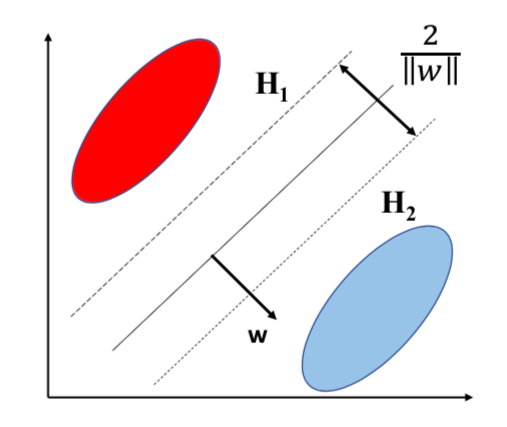
\includegraphics[width = 2in]{margin}
	\caption{SVM}
	\label{fig:margin}
\end{figure}
For any $w$ and $b$, the smallest distance between points and the hyperplane is 
\begin{equation}
\frac{\min_{i} \ell_i(wx_i+b)}{\|w\|_2},
\end{equation} 
where $\ell_i=1-2e_2^Ty_i$.
Note that 
$$
\ell_i=\begin{cases}
1 & \mbox{ if } y_i=\begin{pmatrix}1\\0\end{pmatrix},
\\
-1 &\mbox{ if } y_i=\begin{pmatrix}0\\1\end{pmatrix}.
\end{cases}
$$
Consider the problem
\begin{equation}
	\max_{w,b} \frac{\min_{i} \ell_i(wx_i+b)}{\|w\|_2}.
\end{equation}
Intuitively, the best separating hyperplane $H$ is only determined by those data points who are closest to $H$. Those data points are called {support vector}, and this method are called {support vector machine}.

Without loss of generality, we may restrict the norm of $\|w\|$ to be 1, which leads to a equivalent optimization problem
\begin{equation}
\max_{\|w\|_2 = 1} \min_{i} \ell_i(wx_i+b)
\end{equation}
Actually, {we can prove $\displaystyle \mathop{\rm argmax}_{\|w\|_2 = 1} \min_{i} \ell_i(wx_i+b)$ is nonempty, but here we just admit this fact and only prove the uniqueness of the solution.}

\begin{lemma}
	If $A_1,A_2$ are linearly separable, then
	\begin{equation}\label{binarySVM}
	\mathop{\rm argmax}_{\|w\|_2 = 1} \min_{i} \ell_i(wx_i+b)
	\end{equation}
	is nonempty.
\end{lemma}

\begin{proof}
	Take $x_{i_1} \in A_1$ and  $x_{i_2} \in A_2$,  given $(w,b)\in \{(w,b): l_i(wx_i +b)>0, \forall i\}$, we have
	\begin{equation}
		\begin{cases}
		wx_{i_1} + b > 0,\\
		wx_{i_2} + b < 0
		\end{cases}
	\end{equation}
	which implies $|b| < \max_{i} \|x_i\|_2$. So we have
	\begin{equation}
		\mathop{\rm argmax}_{\|w\|_2 = 1} \min_{i} \ell_i(wx_i+b) = \mathop{\rm argmax}_{\|w\|_2 = 1, ~|b|\leq \max_{i} \|x_i\|_2} \min_{i} \ell_i(wx_i+b) \neq \emptyset.
	\end{equation}
\end{proof}

\begin{lemma}
	If $A_1,A_2$ are linearly separable, then
	\begin{equation}
		\mathop{\rm argmax}_{\|w\|_2 = 1} \min_{i} \ell_i(wx_i+b)
	\end{equation}
	 is a singleton set.
\end{lemma}

\begin{proof}
	Denote $\displaystyle m(w,b) = \min_{i} \ell_i(wx_i+b)$. Notice that $m(w,b)$ is a concave homogeneous function w.r.t $w,b$ and $\|\cdot\|_2$ is a strictly convex norm. Suppose there are two solution $(w_1,b_1)$ and $(w_2,b_2)$ such that $w_1 \neq w_2$, take $\overline{w} = \frac{w_1 + w_2}{2}, \overline{b} = \frac{b_1 + b_2}{2}$, we must have
	\begin{equation}
		m(\overline{w},\overline{b}) \geq \frac{m(w_1,b_1)+ m(w_2,b_2)}{2} = \max_{\|w\|_2 = 1} m(w,b),
	\end{equation}
	and 
	\begin{equation}
		\|\overline{w}\|_2 < 1.
	\end{equation}
	So
	\begin{equation}
		m(\frac{\overline{w}}{\|\overline{w}\|_2},\frac{\overline{b}}{\|\overline{w}\|_2}) = \frac{m(\overline{w},\overline{b}) }{\|\overline{w}\|_2} > \max_{\|w\|_2 = 1} m(w,b),
	\end{equation}
	which leads to a contradiction. So all the solutions must have the same $w$, we denote it as $w^*$. Then if $(w^*,b^*)$ is a solution of problem (\ref{binarySVM}), we must have
	\begin{equation}
		b^* \in \mathop{\rm argmax}_{b} m(w^*,b)
	\end{equation}
	Actually,
	\begin{equation}
		m(w^*,b) = \min\{b+\min_{x\in A_1} w^*x, -b +\min_{x\in A_2} (-w^*x)\}.
	\end{equation}
	It is easy to observe that $\displaystyle \mathop{\rm argmax}_{b} m(w^*,b)$ is a singleton set and 
	\begin{equation}
		b^* = \frac{\min_{x\in A_2} (-w^*x) - \min_{x\in A_1} w^*x}{2}.
	\end{equation}
\end{proof}

Denote
\begin{equation}\label{maxSVM}
	\theta^*_{SVM} = (w_{SVM}^*,b_{SVM}^*) = \mathop{\rm argmax}_{\|w\|_2 = 1} \min_{i} \ell_i(wx_i+b).
\end{equation}


\begin{theorem}[Representation Theorem]
	Let $\theta^*_{SVM} = (w_{SVM}^*,b_{SVM}^*) $ be the solution of \eqref{maxSVM}. Then, $w_{SVM}^*$ must be a linear combination of $x_i^T, i = 1,2,\cdots,N$.
\end{theorem}

\begin{proof}
	Denote
	\begin{equation}
		S = {\rm span} \{x_i^T\}_{i=1}^N.
	\end{equation}
	Then we have
	\begin{equation}
		\mathbb{R}^{1\times d} = S \oplus^{\perp} S^{\perp}.
	\end{equation}
	So $w_{SVM}^*$ can be uniquely decomposed as $w_{SVM}^* = w^*_S + w^*_{S^{\perp}}$ where $w_S\in S$ and $w^*_{S^{\perp}}\in S^{\perp}$. 
	We will prove that $w^*_{S^{\perp}} = 0$. Suppose not, we have
	\begin{equation}
		\|w^*_S\|_2 < \|w_{SVM}^*\|_2 = 1. 
	\end{equation}
	Notice that
	\begin{equation}
		w_{SVM}^* x_i = w_S^* x_i,\ \forall i = 1,2,\cdots,N.
	\end{equation}
	Thus we have
	\begin{equation}
		\min_{i} \ell_i(w_{SVM}^*x_i+b_{SVM}^*) = \min_{i} \ell_i(w_S^*x_i+b_{SVM}^*).
	\end{equation}
	So
	\begin{equation}
	\min_{i} \ell_i(w_{SVM}^*x_i+b_{SVM}^*) < \frac{\min_{i} \ell_i(w_S^*x_i+b_{SVM}^*)}{\|w_S^*\|} = \min_{i} \ell_i(\frac{w^*_S}{\|w_S^*\|_2}x_i+\frac{b_{SVM}^*}{\|w^*_S}\|_2),
	\end{equation}
	which leads to a contradiction to the definition of $\theta_{SVM}^*$.
\end{proof}

%For any $w$ and $b$, the smallest distance between points and the hyperplane is 
%\begin{equation}
%\frac{\min_{i} y_i(wx_i+b)}{\|w\|_2}.
%\end{equation} Consider the problem
%\begin{equation}
%	\max_{w,b} \frac{\min_{i} y_i(wx_i+b)}{\|w\|_2}.
%\end{equation}
%Intuitively, the best separating hyperplane $H$ is only determined by those data points who are closest to $H$. Those data points are called {support vector}, and this method are called {support vector machine}.
%
%Without loss of generality, we may restrict the norm of $\|w\|$ to be 1, which leads to a equivalent optimization problem
%\begin{equation}
%\max_{\|w\|_2 = 1} \min_{i} y_i(wx_i+b)
%\end{equation}
%Actually, {we can prove $\displaystyle \mathop{\rm argmax}_{\|w\|_2 = 1} \min_{i} y_i(wx_i+b)$ is nonempty, but here we just admit this fact and only prove the uniqueness of the solution.}
%
%\begin{lemma}
%	If $A_1,A_2$ are linearly separable, then
%	\begin{equation}\label{binarySVM}
%		\mathop{\rm argmax}_{\|w\|_2 = 1} \min_{i} y_i(wx_i+b)
%	\end{equation}
%	 is a singleton set.
%\end{lemma}
%
%\begin{proof}
%	Denote $\displaystyle m(w,b) = \min_{i} y_i(wx_i+b)$. Notice that $m(w,b)$ is a concave homogeneous function w.r.t $w,b$ and $\|\cdot\|_2$ is a strictly convex norm. Suppose there are two solution $(w_1,b_1)$ and $(w_2,b_2)$ such that $w_1 \neq w_2$, take $\overline{w} = \frac{w_1 + w_2}{2}, \overline{b} = \frac{b_1 + b_2}{2}$, we must have
%	\begin{equation}
%		m(\overline{w},\overline{b}) \geq \frac{m(w_1,b_1)+ m(w_2,b_2)}{2} = \max_{\|w\|_2 = 1} m(w,b),
%	\end{equation}
%	and 
%	\begin{equation}
%		\|\overline{w}\|_2 < 1.
%	\end{equation}
%	So
%	\begin{equation}
%		m(\frac{\overline{w}}{\|\overline{w}\|_2},\frac{\overline{b}}{\|\overline{w}\|_2}) = \frac{m(\overline{w},\overline{b}) }{\|\overline{w}\|_2} > \max_{\|w\|_2 = 1} m(w,b),
%	\end{equation}
%	which leads to a contradiction. So all the solutions must have the same $w$, we denote it as $w^*$. Then if $(w^*,b^*)$ is a solution of problem (\ref{binarySVM}), we must have
%	\begin{equation}
%		b^* \in \mathop{\rm argmax}_{b} m(w^*,b)
%	\end{equation}
%	Actually,
%	\begin{equation}
%		m(w^*,b) = \min\{b+\min_{x\in A_1} w^*x, -b +\min_{x\in A_2} (-w^*x)\}.
%	\end{equation}
%	It is easy to observe that $\displaystyle \mathop{\rm argmax}_{b} m(w^*,b)$ is a singleton set and 
%	\begin{equation}
%		b^* = \frac{\min_{x\in A_2} (-w^*x) - \min_{x\in A_1} w^*x}{2}.
%	\end{equation}
%\end{proof}
%
%Denote
%\begin{equation}\label{maxSVM}
%	\theta^*_{SVM} = (w_{SVM}^*,b_{SVM}^*) = \mathop{\rm argmax}_{\|w\| = 1} \min_{i} y_i(wx_i+b).
%\end{equation}
%
%
%\begin{theorem}[Representation Theorem]
%	Let $\theta^*_{SVM} = (w_{SVM}^*,b_{SVM}^*) $ be the solution of \eqref{maxSVM}. Then, $w_{SVM}^*$ must be a linear combination of $x_i^T, i = 1,2,\cdots,N$.
%\end{theorem}
%
%\begin{proof}
%	Denote
%	\begin{equation}
%		S = {\rm span} \{x_i^T\}_{i=1}^N.
%	\end{equation}
%	Then we have
%	\begin{equation}
%		\mathbb{R}^{1\times d} = S \oplus^{\perp} S^{\perp}.
%	\end{equation}
%	So $w_{SVM}^*$ can be uniquely decomposed as $w_{SVM}^* = w^*_S + w^*_{S^{\perp}}$ where $w_S\in S$ and $w^*_{S^{\perp}}\in S^{\perp}$. 
%	We will prove that $w^*_{S^{\perp}} = 0$. Suppose not, we have
%	\begin{equation}
%		\|w^*_S\|_2 < \|w_{SVM}^*\|_2 = 1. 
%	\end{equation}
%	Notice that
%	\begin{equation}
%		w_{SVM}^* x_i = w_S^* x_i,\ \forall i = 1,2,\cdots,N.
%	\end{equation}
%	Thus we have
%	\begin{equation}
%		\min_{i} y_i(w_{SVM}^*x_i+b_{SVM}^*) = \min_{i} y_i(w_S^*x_i+b_{SVM}^*).
%	\end{equation}
%	So
%	\begin{equation}
%	\min_{i} y_i(w_{SVM}^*x_i+b_{SVM}^*) < \frac{\min_{i} y_i(w_S^*x_i+b_{SVM}^*)}{\|w_S^*\|} = \min_{i} y_i(\frac{w^*_S}{\|w_S^*\|_2}x_i+\frac{b_{SVM}^*}{\|w^*_S}\|_2),
%	\end{equation}
%	which leads to a contradiction to the definition of $\theta_{SVM}^*$.
%\end{proof}

\subsection{Soft margin maximization and kernel methods}

We may rewrite the SVM problem as
\begin{align} 
	\max_{w,b}&\ {2\over \|w\|},\\
	s.t.&\ \ell_i(wx_i+b) \geq 1,\ \forall i. 
\end{align}
or equivalently,
\begin{align}{\label{SVM_Quad}}
	\min_{w,b}&\ \|w\|^2,\\
	s.t.&\ \ell_i(wx_i+b) \geq 1,\ \forall i. 
\end{align}
Notice that the feasible domain of margin maximization is nonempty if and only if dataset is linearly separable. So when the data is linearly nonseparable, this method can't even get a classifier even though it may not be good. One way to handle this problem is to relax the constraint by adding relaxation variables. 

Define soft margin maximization problem
\begin{align}{\label{SVM_Quad_soft}}
\min_{w,b,\xi}&\ \|w\|^2 + \lambda^{-1} \sum_{i = 1}^N\xi_i,\\
s.t.&\ \ell_i(wx_i+b) + \xi_i \geq 1,\ \forall i. \\
     &\ \xi_i \geq 0.
\end{align}
where $\lambda>0$. The above problem is equivalent to
 \begin{align}
 \min_{w,b}&\ \|w\|^2 + \lambda^{-1} \sum_{i = 1}^N {\rm ReLU}(1-\ell_i(wx_i+b)).
 \end{align}
Thus, soft margin maximization problem \eqref{SVM_Quad_soft} can be reformulated as
 \begin{align}{\label{SVM_soft}}
\min_{w,b}&\  \sum_{i = 1}^N {\rm ReLU}(1-\ell_i(wx_i+b)) + \lambda \|w\|^2.
\end{align}
We can still prove that the solution of (\ref{SVM_soft}) satisfies the representation theorem. Thus we can restrict $w$ to be in the set $S$. Assume that  
\begin{equation}
	w = \sum_{i = 1}^N \alpha_i x_i^T, 
\end{equation}
Denote $\alpha = (\alpha_1,\cdots,\alpha_N)^T$. We can rewrite the problem (\ref{SVM_soft}) as 
\begin{equation}
\min_{\alpha}\ \sum_{i = 1}^N {\rm ReLU}(1-\ell_i(\sum_{j = 1}^N \langle x_i,x_j\rangle \alpha_j+b)) + \lambda\alpha^T \big(\langle x_i,x_j\rangle\big)_{N\times N} \alpha\\
\end{equation}
We can see that the whole problem is only determined by the inner product of data points but not the data itself directly. \\

Use the above formulation, we can induce nonlinearity in SVM. Denote the input space as $X$ where $\{x_i\}_{i=1}^N \subset X$. We use two steps to obtain a nonlinear classification model. First, we use a nonlinear feature mapping $\phi: X\rightarrow \mathcal{H}$ to map input space $X$ to a feature space $\mathcal{H}$. Second, we use linear SVM to do classification on $\{\phi(x_i)\}_{i=1}^N\subset \mathcal{H}$.\\

We may just asssume dataset after feature mapping $\phi$ is linearly separable. Then, the SVM problem after doing feature mapping can be formulated as
problem (\ref{SVM_soft}) as 
\begin{equation}
\min_{\alpha}\ \sum_{i = 1}^N {\rm ReLU}(1-\ell_i(\sum_{j = 1}^N \langle \phi(x_i),\phi(x_j)\rangle \alpha_j+b)) + \lambda\alpha^T \big(\langle \phi(x_i),\phi(x_j)\rangle\big)_{N\times N} \alpha\\
\end{equation}

Notice that to obtain the above problem we don't really need to know what exactly is the nonlinear mapping $\phi$, but only need to compute the value of $<\phi(x_i),\phi(x_j)>$. So we define a kernel function $k: X\times X\rightarrow \mathbb{R}$ such that 
\begin{equation}
	k(x,y) = \langle\phi(x),\phi(y)\rangle,\ x,y\in X.
\end{equation}
Then the kernel SVM can be formulated as
\begin{equation}
\min_{\alpha}\ \sum_{i = 1}^N {\rm ReLU}(1-\ell_i(\sum_{j = 1}^N  k(x_i,x_j) \alpha_j+b)) + \lambda\alpha^T \big(k(x_i,x_j)\big)_{N\times N} \alpha\\
\end{equation}
In practice, we just need to find a proper kernel function instead of a good nonlinear feature mapping. Here we list some common used kernel functions:
\begin{itemize}
	\item Polynomial kernel: $k(x,y) = (a\langle x,y\rangle+ b)^n, a > 0, b\geq 0, n\in \mathbb{N}^+$.
	\item Gaussian kernel: $k(x,y) = e^{-\gamma\|x-y\|^2}, \gamma > 0$.
	\item Laplacian kernel: $k(x,y) = e^{-\gamma\|x-y\|}, \gamma > 0$
	\item Tanh kernel: $k(x,y) = \tanh(a\langle x,y\rangle+b), a>0, b\geq 0.$
\end{itemize}

\subsection{Binary logistic regression}
In multi-class Logistic regression, if we use $\|W\|$ to replace $\|\bm\theta\|$ in regularization term,  we can get another version of logistic regression:
\begin{equation}
	\mathcal L_\lambda(\bm \theta) = - \sum_{i=1}^k \sum_{x\in A_i} \log p_{i}(x;\bm \theta) + \lambda R(\|W\|),
\end{equation}
where $p_i(x;\bm \theta)$ and $R(\cdot)$ share the same definitions as in previous sections of logistic regression.
Let  
\begin{equation}
\bm\Theta_{\lambda} = \mathop{{\arg\min}}_{\bm\theta}  \mathcal L_\lambda(\bm\theta).
\end{equation}
The following lemma follows directly from the definition of $p_{i}(x;\bm \theta)$.
\begin{lemma}
	For any $W\in \mathbb{R}^{k\times d}, b\in \mathbb{R}^k, \alpha \in \mathbb{R}$, we have
	\begin{equation}
		\mathcal L_\lambda(W,b) = \mathcal L_\lambda(W,b + \alpha \bm 1),
	\end{equation}
	where $\bm 1 = (1,1,\cdots,1)^T\in\mathbb{R}^k.$
\end{lemma}

Binary logistic regression refers to the case when $k=2$.
\begin{lemma}
	If $k = 2$, given any $\bm\theta_\lambda = \begin{pmatrix}
	w_1 &  b_1\\
	w_2 & b_2 
	\end{pmatrix} \in \bm\Theta_\lambda$, we have
	\begin{equation*}
         w_1 = -w_2.
	\end{equation*}
\end{lemma}

According to the above two lemmas, we can restrict $\bm\theta$ to have the form
\begin{equation}
	\bm\theta = \begin{pmatrix}
	\frac{w}{2}\ &\frac{b}{2}\\
	-\frac{w}{2}\ &-\frac{b}{2}
	\end{pmatrix},
\end{equation}
so our score mapping can be written as
\begin{equation}\label{key}
\bm p(x;\theta) = \begin{pmatrix} 
	\frac{1}{1+ e^{-(wx+b)}}\\
	\frac{1}{1+e^{wx+b}}
\end{pmatrix}.
\end{equation}
Denote $\theta = (w,b)$ where $w\in \mathbb{R}^d, b\in \mathbb{R}$, correspondingly, we have
\begin{equation}
P(\theta) = \prod_{i = 1}^N \frac{1}{1+ e^{-y_i(wx+b)}}.
\end{equation}
Here we have the new ``label'' $y_i$ defined by
\begin{equation}\label{key}
y_i = \begin{cases}
1, \quad &\text{if}  \quad x_i \in A_1 \\
-1, \quad &\text{if} \quad x_i \in A_2
\end{cases}.
\end{equation}
Thus we have
\begin{equation}
L(\theta) = -\log P(\theta) = \sum_{i = 1}^N \log(1+ e^{-y_i(wx+b)}),
\end{equation}
and take $R(t) = t^2$, we have
\begin{equation}
\mathcal L_{\lambda}(\theta)  = L(\theta) + \lambda \|w\|_2^2 = \sum_{i = 1}^N \log(1+ e^{-y_i(wx+b)}) + \lambda \|w\|_2^2.
\end{equation}
Here $L(\theta)$ is a strictly convex function without any global minima. 


\begin{lemma}
Assume that $A_1,A_2$ are linearly separable, and we follow the same definition
of linearly classifiable weights:
\begin{equation}
\bm{\Theta} = \left\{\bm\theta: p_i(x; \bm\theta)>p_j(x; \bm\theta),~\forall x\in A_i, j\neq i, i= 1,2\right\},
\end{equation}
where 
\begin{equation}\label{key}
\bm p(x;\theta) = \begin{pmatrix} 
\frac{1}{1+ e^{-(wx+b)}}\\
\frac{1}{1+e^{wx+b}}
\end{pmatrix}.
\end{equation}
Then, we have the following statement:\\

\begin{enumerate}

\item  $\theta = (w,b) \in \Theta$ if and only if
		\begin{equation*}
		\frac{1}{1+ e^{-y_i(wx+b)}} > \frac{1}{2},\ \forall i = 1,2\cdots,N.
		\end{equation*} 
\item  If $P(\theta) > \frac{1}{2}$, then $\theta$ must be classifiable, i.e.
\begin{equation*}
	\{\theta: P(\theta)>\frac{1}{2}\}\subset \bm \Theta.
\end{equation*}
\item  Prove that
\begin{equation*}
	\bm\Theta = \{\theta: \lim_{\alpha\rightarrow +\infty} P(\alpha \theta) = 1\}.
\end{equation*}
\end{enumerate}
\end{lemma}

 
 
	If $A_1,A_2$ are linearly separable, then
$\displaystyle 
\mathop{\rm argmin}_{w,b} \mathcal L_{\lambda}(\theta)
$
	is nonempty for $\lambda $ sufficiently small.


\begin{lemma}
		If $A_1,A_2$ are linearly separable, then
	\begin{equation}\label{binaryLR}
	\mathop{\rm argmin}_{w,b} \mathcal L_{\lambda}(\theta)
	\end{equation}
	is a singleton set for $\lambda $ sufficiently small.
\end{lemma}

\begin{proof}
Because $L(\theta)$ is strictly convex w.r.t. $\theta$ and $\|w\|^2$ is convex w.r.t. $\theta$, so $\mathcal L(\theta,\lambda)  = L(\theta) + \lambda \|w\|_2^2$ is stricly convex w.r.t. $\theta$, which implies our result directly.

\end{proof}

For $\lambda$ sufficiently small, denote
\begin{equation}
	\theta_{LR}(\lambda) = (w_{LR}(\lambda),b_{LR}(\lambda)) = \mathop{\rm argmin}_{w,b} \mathcal L_{\lambda}(\theta).
\end{equation}

\begin{lemma}
	If $A_1,A_2$ are linearly separable,  
	\begin{enumerate}
	\item $\mathcal L_{\lambda}(\theta) \rightarrow 0$ as $\lambda \rightarrow 0$.
	\item $\|w_{LR}(\lambda)\|\rightarrow \infty$ as $\lambda \rightarrow 0$.
	\item $\displaystyle \min_{i} y_i(w_{LR}(\lambda) x_i + b_{LR}(\lambda))\rightarrow \infty$ as $\lambda \rightarrow 0$.
	\item If $A_1,A_2$ are also nonempty, 
	\begin{equation}
		\|b_{LR}(\lambda)\|\leq \max_{i} \|x_i\| \|w_{LR}(\lambda)\|
	\end{equation}
	for $\lambda$ sufficiently small.
	\end{enumerate}
\end{lemma}

The above lemma implies that $\theta_{LR}(\lambda)/\|w_{LR}(\lambda)\|$ is bounded for $\lambda$ sufficiently small.

\begin{theorem}
	If $A_1,A_2$ are linearly separable, then $\frac{\theta_{LR}(\lambda)}{\|w_{LR}(\lambda)\|}$ converge to $\theta^*_{SVM}$ as $\lambda \rightarrow 0$, i.e.
	\begin{equation}
		\theta^*_{SVM} = \lim_{\lambda\rightarrow 0} \frac{\theta_{LR}(\lambda)}{\|w_{LR}(\lambda)\|}.
	\end{equation}
\end{theorem}

\begin{proof}
	Because $\frac{\theta_{LR}(\lambda)}{\|w_{LR}(\lambda)\|}$ is bounded for $\lambda$ sufficiently small, we only need to prove that it has no convergence points other than $\theta^*_{SVM}$ as $\lambda \rightarrow 0$.\\
	We first introduce a soft margin function $m: \mathbb{R}^n \rightarrow \mathbb{R}$ such that 
	\begin{equation}
		m(\theta) = \min_{i} y_i(wx_i + b).
	\end{equation}
	Suppose that there exist a sequence $\{\lambda_n\}_{n = 1}^\infty$ and $\bar{\theta} = (\bar{w},\bar{b}) \neq \theta^*_{SVM}$ so that  $\lambda_n \downarrow 0$ and $\frac{\theta_{LR}(\lambda_n)}{\|w_{LR}(\lambda_n)\|} \rightarrow \bar{\theta}$ as $n\rightarrow \infty$. Obviously $\|\bar{w}\| = 1$, and 
    \begin{equation}
    	0 \leq m(\bar{\theta}) < m(\theta^*_{SVM}).
    \end{equation}
     Take a positive number $\epsilon < m(\theta^*_{SVM}) - m(\bar{\theta})$. Then there exists $K_0\in \mathbb{N}^+$ such that 
    \begin{equation}
    0 < m(\frac{\theta_{LR}(\lambda_n)}{\|w_{LR}(\lambda_n)\|}) <  m(\theta^*_{SVM})- \epsilon,
    \end{equation}
    for all $n \geq K_0$.\\
    
    Consider $\theta_n = (w_n,b_n) = \|w_{LR}(\lambda_n)\|\theta^*_{SVM}$. Then
    \begin{equation}
    \lim_{n\rightarrow \infty} \frac{\log(1 + e^{-m(\theta_n)})}{\log(1 + e^{-m(\theta_{LR}(\lambda_n))}} = \lim_{n \rightarrow \infty} e^{\|w_{LR}(\lambda_n)\| (m(\frac{\theta_{LR}(\lambda_n)}{\|w_{LR}(\lambda_n)\|}) -  m(\theta^*_{SVM}))} \leq \lim_{n \rightarrow \infty} e^{-\|w_{LR}(\lambda_n)\| \epsilon} = 0.
    \end{equation}
    So there exists a $K_1 \in \mathbb{N}^+$ such that 
    \begin{equation}
    	N \log(1 + e^{-m(\theta_n)}) < \log(1 + e^{-m(\theta_{LR}(\lambda_n))}) 
    \end{equation}
    for all $n \geq K_1$. Take $K  = \max\{K_0, K _1\}$. Then for all $n \geq K$, we have 
    \begin{equation}
    	\mathcal{L}(\theta_n) \leq N \log(1 + e^{-m(\theta_n)}) + \lambda \|w_{\lambda_n}\|^2 < \log(1 + e^{-m(\theta_{LR}(\lambda_n))})+ \lambda \|w_{\lambda_n}\|^2 \leq \mathcal{L}(\theta_{LR}(\lambda_n)),
    \end{equation} 
    which contradicts the definition of $\theta_{LR}(\lambda)$.
\end{proof}


For the proof of the above theorem, you can also refer to the paper by Rosset Saharon, Zhu Ji and Trevor J. Hastie~ \cite{rosset2004margin}. 

%\section{Numerical examples}
In this section, we will list some numerical results using different methods on the MNIST dataset. 

%The MNIST data set contains the pictures of single digits. The size of each digit picture is 28*28 and the label is the digit from 0 to 9. There are 60000 training data and 10000 test data in all.
\subsection{Least square}

We first present the details of the experiments using the least square for classification. 

The most straightforward model for prediction is the linear model
$$
y=Wx+b,
$$
where $x\in \mathbb{R}^{784}$ is the input data, $y\in \mathbb{R}^{10}$ is the prediction and $W \in \mathbb{R}^{10 \times 784}, b \in \mathbb{R}^{10} $ are the parameters of the model. 
For each data in the MNIST dataset, $x_i\in \mathbb{R}^{784}, i=1,...,60000$, denote the corresponding label as $y_i\in \mathbb{R}^{10}$. 
We denote the training set and labels in matrix form, 
$$A=\begin{pmatrix}
    x_{1} &x_{2}  &...  &x_{60000}     \\
    1&1&... &1\\
\end{pmatrix}^T \in \mathbb{R}^{60000\times 785},$$ 
$$Y=\begin{pmatrix}
    y_{1}        ,
    y_{2}       ,
    ... ,
    y_{60000}     
\end{pmatrix}^T\in \mathbb{R}^{60000\times 10}.
$$
Our goal is to find the optimal parameter 
$\theta=\left[ W ,b  \right]^T\in \mathbb{R}^{785\times 10}$ to minimize the total sum of square loss 
$$
\sum_{i=1}^{60000} \|y_i-(W x_i+b)\|^2_2=\|Y- A\theta\|^2_2.
$$
The empirical formulae gives the optimal parameter as
\begin{align}
\hat{\theta}=(A^TA)^{-1}A^TY.
\end{align}


For the MNIST dataset, after $\hat{\theta}$ is calculated, we can classify $x_i$ based on the linear model
\begin{align}
\hat{y_i}=\hat{W}x_i+\hat{b} \in \mathbb{R}^{10}.
\end{align}
We choose the entry in $\hat{y_i}$ with the maximum value as the predicted label for $x_i$. Finally, the training accuracy is 85.77$\%$ and the test accuracy is 86.03$\%$. 

\subsection{Logistic regression }
The model of logistic regression is slightly different from least square in the prediction and the loss function. With similar notations, we use $\hat{y}$=softmax($Wx+b$) as the predicted label of the input.
Here there is one more operation of softmax in the predicted label of an input $x$. It is used for normalizing the output to a probability distribution. Moreover, the loss function here is the cross entropy loss with an $\ell^2$ regularization term
\begin{align}
L_{\lambda}(\theta)=L(\theta)+\lambda R(\|\theta\|)=
-(y \log(\hat{y})+(1-y)\log(1-\hat{y}))
+\lambda \|\theta\|^2.
\end{align}
We use the {\color{red}Adam} optimization algorithm in the numerical experiment. We choose the learning rate to be 0.001,  batch size to be 100
and regularization coefficient to be 0.0001 for 50 training epochs. Finally, the training accuracy is 93.46$\%$ and the test accuracy is 92.56$\%$. 




\subsection{Support vector machine (SVM) }
Finally, we use SVM for classification which we discussed in Section \ref{sec:SVMintro}. The main hypercoefficient is the kernel to be used in the algorithm. There are many kernels available such as linear kernel, Gaussian kernel, polynomial kernel and so on. We recall these kernels here. 
\begin{itemize}
	\item Polynomial kernel: $k(x,y) = (a\langle x,y\rangle+ b)^n, a > 0, b\geq 0, n\in \mathbb{N}^+$.
	\item Gaussian kernel: $k(x,y) = e^{-\gamma\|x-y\|^2}, \gamma > 0$.
\end{itemize}
We choose the regularization parameter $\lambda=1$ in \eqref{SVM_Quad_soft} and use polynomial kernel 
and Gaussian kernel as well as no kernel 
for numerical experiments. 
With no kernel, the training accuracy is 87.91$\%$ and the test accuracy is 87.73$\%$. 
With polynomial kernel, the training accuracy is 99.16$\%$ and the test accuracy is 97.71$\%$. 
With Gaussian kernel, the training accuracy is 98.99$\%$ and the test accuracy is 97.92$\%$.

%The training accuracy is 99.16$\%$ and the test accuracy is 97.71$\%$.

\subsection{Summary }
For the dataset of MNIST, the traditional linear machine learning models can achieve good classification accuracy. 

  If we apply standard least square to the  MNIST dataset, we only get 86.03\% test accuracy. If we apply logistic regression to the  MNIST dataset, we get 92.56\% test accuracy. If we apply support vector machine (SVM) with polynomial kernel to the  MNIST dataset, we get 97.71\% test accuracy. If we apply support vector machine (SVM) with Gaussian kernel to the  MNIST dataset, we get 97.92\% test accuracy. 

\begin{table}[!htbp]
	\begin{center}
		\begin{tabular}{|c|c|c|}
			\hline
			Model &  Training accuracy(\%)   &   Test accuracy(\%) \\
			\hline
			Least square & 85.77	           &   86.03 \\ \hline
			Logistic regression & 93.46   &   92.56	     \\ \hline
			SVM without kernel& 87.91           &   87.73         \\	\hline
			SVM with kernel& 99.16            &   97.71         \\	\hline
			CNN & 99.99            &   99.79         \\	\hline
		\end{tabular}
	\end{center}
	\caption{Training and test accuracy of different models on MNIST.}
	\label{tab:MNIST-LR-Results}
\end{table}


\begin{table}[!htbp]
	\begin{center}
		\begin{tabular}{|c|c|c|}
			\hline
			Model &  Training accuracy(\%)   &   Test accuracy(\%) \\
			\hline
			Least square & 45.10           &   32.86 \\ \hline
			Logistic regression & 39.25   &   35.23	     \\ \hline
			SVM without kernel& 33.02            &   23.76         \\	\hline
			SVM with kernel& 70.29            &   54.37         \\	\hline
			CNN & 99.97            &   95.05         \\	\hline
		\end{tabular}
	\end{center}
	\caption{Training and test accuracy of different models on CIFAR-10.}
	\label{tab:MNIST-LR-Results2}
\end{table}
In the meanwhile, the accuracy of the state-of-art CNN model (see more details in Section \ref{sec:CNNs})applied on the MNIST dataset is 99.79\%. We summarize the accuracy of these models on MNIST in the following Table \ref{tab:MNIST-LR-Results}.

In the following Table \ref{tab:MNIST-LR-Results2}, we summarize the accuracy of different models on CIFAR-10.

Based on the previous results, CNN models outperform all the other models significantly. 
Thus we want to investigate the convolutional neural networks for better performance rather than the traditional machine learning models. 

%\section{Finite element discretization for Poisson equation}
\chapter{Convolutional Multigrid Method}
%%%%%%%%%%%%%%%%%%%%%%%%%%%%%%%%%%
%\section{Two-point boundary problems and finite element discretization}
Denote the functional space
$$
V:=H^1_0(0,1)=\{v:\, [0,1]\rightarrow R,\,\,\mbox{$v$ is continuous and}\, v(0)=v(1)=0\}.
$$
Given any $f: [0,1]\rightarrow R$, consider 
\begin{equation*}
J(v)=\frac12\int_{0}^1|v'|^2dx-\int_{0}^1 fvdx.
\end{equation*}
Find $u\in V$ such that 
\begin{equation}\label{minvar}
\displaystyle u=\argmin_{v\in V} J(v)\quad
\end{equation}
\begin{theorem}
Problem \eqref{minvar} is equivalent to: Find $u\in V$ such that 
\begin{equation}\label{1Dpossion}
\left\{
\begin{aligned}
-u''&= f, \,\, 0<x<1, \\
 u(0)&=u(1)=0.
\end{aligned}
\right.
\end{equation}
\end{theorem}
\begin{proof}
For any $v\in V, t\in R$, let $g(t)=J(u+t v)$. 
Since $u=\argmin_{v\in V} J(v)$ means $g(t)\ge g(0)$. Hence, for any $v\in V$, $0$ is the global minimum of the function $g(t)$. Therefore
$g'(0)=0$ implies 
$$
\int_{0}^1 u'v'dx=\int_0^1fvdx\quad \forall v\in V. 
$$
By integration by parts, which is equivalent to 
$$
\int_{0}^1 (-u''-f)vdx=0\quad \forall v\in V. 
$$
It can be proved that the above identity holds if and only if 
$-u''= f$ for all $x\in (0,1)$. Namely $u$ satisfies \eqref{1Dpossion}. 
\end{proof}

Let $V_h$ be finite element space and $\{\varphi_1, \varphi_2, \cdots \varphi_{n}\}$ be a nodal basis of $V_h$. 
%Let $\{\psi_1,\psi_2,\cdots, \psi_{n}\}$ be a dual basis of $\{\varphi_1, \varphi_2, \cdots \varphi_{n}\}$, namely $(\varphi_i,\psi_j )=\delta_{ij}$.
\begin{equation}
J(v_h)=\frac12\int_0^1|v_h'|^2dx-\int_0^1fv_hdx.
\end{equation}
Let 
$$
\displaystyle v_h=\sum_{i=1}^{n}\nu_i\varphi_i,\quad \nu=(\nu_i)_{i=1}^{n}
$$
then using the convolution notation, we have
$$
J(v_h)=I(\nu)=\frac12\nu^TA\ast\nu-b^T\nu
$$
and 
$$
\nabla I(\nu) =A\ast \nu -b,
$$
where $A=\frac{1}{h}[-1,2, -1]$.

At the same time, let $\displaystyle u_h=\sum_{i=1}^{n}\mu_i\varphi_i,$
\begin{equation}\label{min1d}
\displaystyle u_h=\argmin_{v_h\in V_h} J(v_h)\Leftrightarrow \mu=\argmin_{\nu \in R^n} I(\nu)
\end{equation}
And $u_h$ solves the problem: Find $u_h\in V_h$
\begin{equation}\label{1ddiscrevar}
\frac{d}{dt}J(u_h+t v_h)|_{t=0}=a(u_h,v_h)-\langle f, v_h\rangle=0 \quad \forall v_h\in V_h. 
\end{equation}
where 
$$
a(u_h,v_h)=\int_0^1 u_h'v_h'dx.
$$

\begin{theorem}\label{thm:best-approximation}
Let $V$ be a Hilbert space, $a(\cdot,\cdot)$ be a continuous,
symmetric, bilinear form defining an inner product on $V$. Let
$f(\cdot)$ be a continuous linear form. If $u$ is solution to the
problem~\eqref{minvar} and $u_h$ is a solution
to~\eqref{min1d}, then the following equality holds:
\begin{equation}\label{eq:best-approx}
\|u-u_h\|_a = \inf_{v\in V_h}\|u-v\|_a,
\end{equation}
where $\|u-u_h\|^2_a = a(u-u_h,u-u_h)$. 
\end{theorem}

\begin{proof}
Frist, one sees that
$$
a(u-u_h, v)=0,~~~\forall v\in V_h.
$$
Thus, for any $v\in V_h$ we have
\begin{eqnarray*}
& &\|u-u_h\|_a^2=a(u-u_h, u-u_h)\\[0.2cm]
&=& a(u-u_h, u-v)\\[0.2cm]
&\le& \|u-u_h\|_a\|u-v\|_a.
\end{eqnarray*}
Taking the infimum on both sides of this equation then gives. 
$$
\|u-u_h\|_a\le \inf_{v\in V_h}\|u-v\|_a.
$$
The proof is complete, since 
\[
\|u-u_h\|_a\ge \inf_{v\in V_h}\|u-v\|_a,
\]
by the definition of infimum. 
\end{proof}
Combining Theorem \ref{interp00} and Theorem \ref{thm:best-approximation}, we obtain the error estimate for the finite element method. 
\begin{theorem}
If $u\in H^2(\Omega)$ is solution to the
problem~\eqref{1Dpossion} and $u_h$ is a solution to~\eqref{min1d}, then we have:
\begin{equation}
 \|u-u_h\|+h |u-u_h|_{1}\lc h^2 |u|_2.
   \end{equation}
 \end{theorem}



%\subsection{Gradient descent method}

Using the convolution notation \eqref{con010}, we consider
$$
J(v_h)=I(\nu)=\frac12\nu^TA\ast\nu-b^T\nu
$$
and 
$$
\nabla I(\nu) =A\ast \nu -b,
$$
where $A=\frac{1}{h}[-1,2, -1]$.

At the same time, let $\displaystyle u_h=\sum_{i=1}^n\mu_i\varphi_i,$
\begin{equation}\label{min}
\displaystyle u_h=\argmin_{v_h\in V_h} J(v_h)\Leftrightarrow \mu=\argmin_{\nu \in R^n} I(\nu)
\end{equation}

Noting that $\nabla I(\nu) =A\ast \nu -b$ and applying the gradient descent method to solve problem \eqref{min}, we obtain 
$$
\mu^{(m)}=\mu^{(m-1)}-\eta(A\ast \mu^{(m-1)}-b),\quad m=1,\cdots,\nu. 
$$
After $\nu$ iterations of gradient descent method, we denote the solution as $u_h^{\nu}$.

Consider the finite element discretization of Poisson equation in 1D: One very simple iterative method for \eqref{min} is the following
gradient descent method
$$
       \mu^{(m)}=\mu^{(m-1)}+\eta (b-A\ast \mu^{(m-1)}),
$$
or, for $j=1:N$, 
$$ 
\mu^{(m)}_j=\mu^{(m-1)}_j+\eta
\bigg(\beta_j-\frac{-\mu^{(m-1)}_{j-1}+2\mu^{(m-1)}_j-\mu^{(m-1)}_{j+1}}{h}\bigg),
$$
where $\eta>0$ is a positive parameter named learning rate.  

It is not so difficult to
properly choose $\eta$ so that the above iterative scheme converges,
namely for any initial guess $\mu^0$, the sequence $(\mu^{(m)})$ generated
by the above iteration converges to the exact solution $\mu$ of
\eqref{min}.

Note that
$$
        \mu=\mu+\eta (b-A\ast\mu),
$$
we get
$$
        \mu-\mu^{(m)}=(I-\eta A\ast)(\mu-\mu^{(m-1)}),
$$
or
$$
        \mu-\mu^{(m)}=(I-\eta A\ast)^m(\mu-\mu^0), m=1,2,3,\cdots
$$
As we known,
$$
(I-\eta A\ast)^m\longrightarrow 0
$$
if and only if $\rho (I-\eta A\ast)<1$. Here $\rho(B)$ is the spectral 
radius of $B$. However, $\rho (I-\eta A\ast)<1$ if and only if
$$
0< \mbox{all the eigenvalue of}~ A\ast< 2\eta^{-1}.
$$
Thus, a necessary and sufficient condition for the 
convergence is the following
$$
       0< \eta<{2\over \rho(A\ast)}.
$$
It is easy to see that
(for example, $4/h$ is an upper bound of its row sums)
$$
{4\over {h}}> \rho(A\ast).
$$
Therefore it is reasonable to make the following choice
$$
        \eta={h \over 4}
$$
and the resulting algorithm is 
\begin{equation}\Label{1dRichardson}
        \mu^{(m)}=\mu^{(m-1)}+{h\over4} (b-A\ast\mu^{(m-1)}).
\end{equation}
In the rest of this section, unless otherwise noted, we shall choose
$\eta$ as above for simplicity.

On Figure~\ref{fig:richardson} the convergence history plot of the
above gradient descent iterative method for typical application is shown.
As we see, this iterative scheme converges very slowly.

\begin{figure}[!htb]
\begin{center}
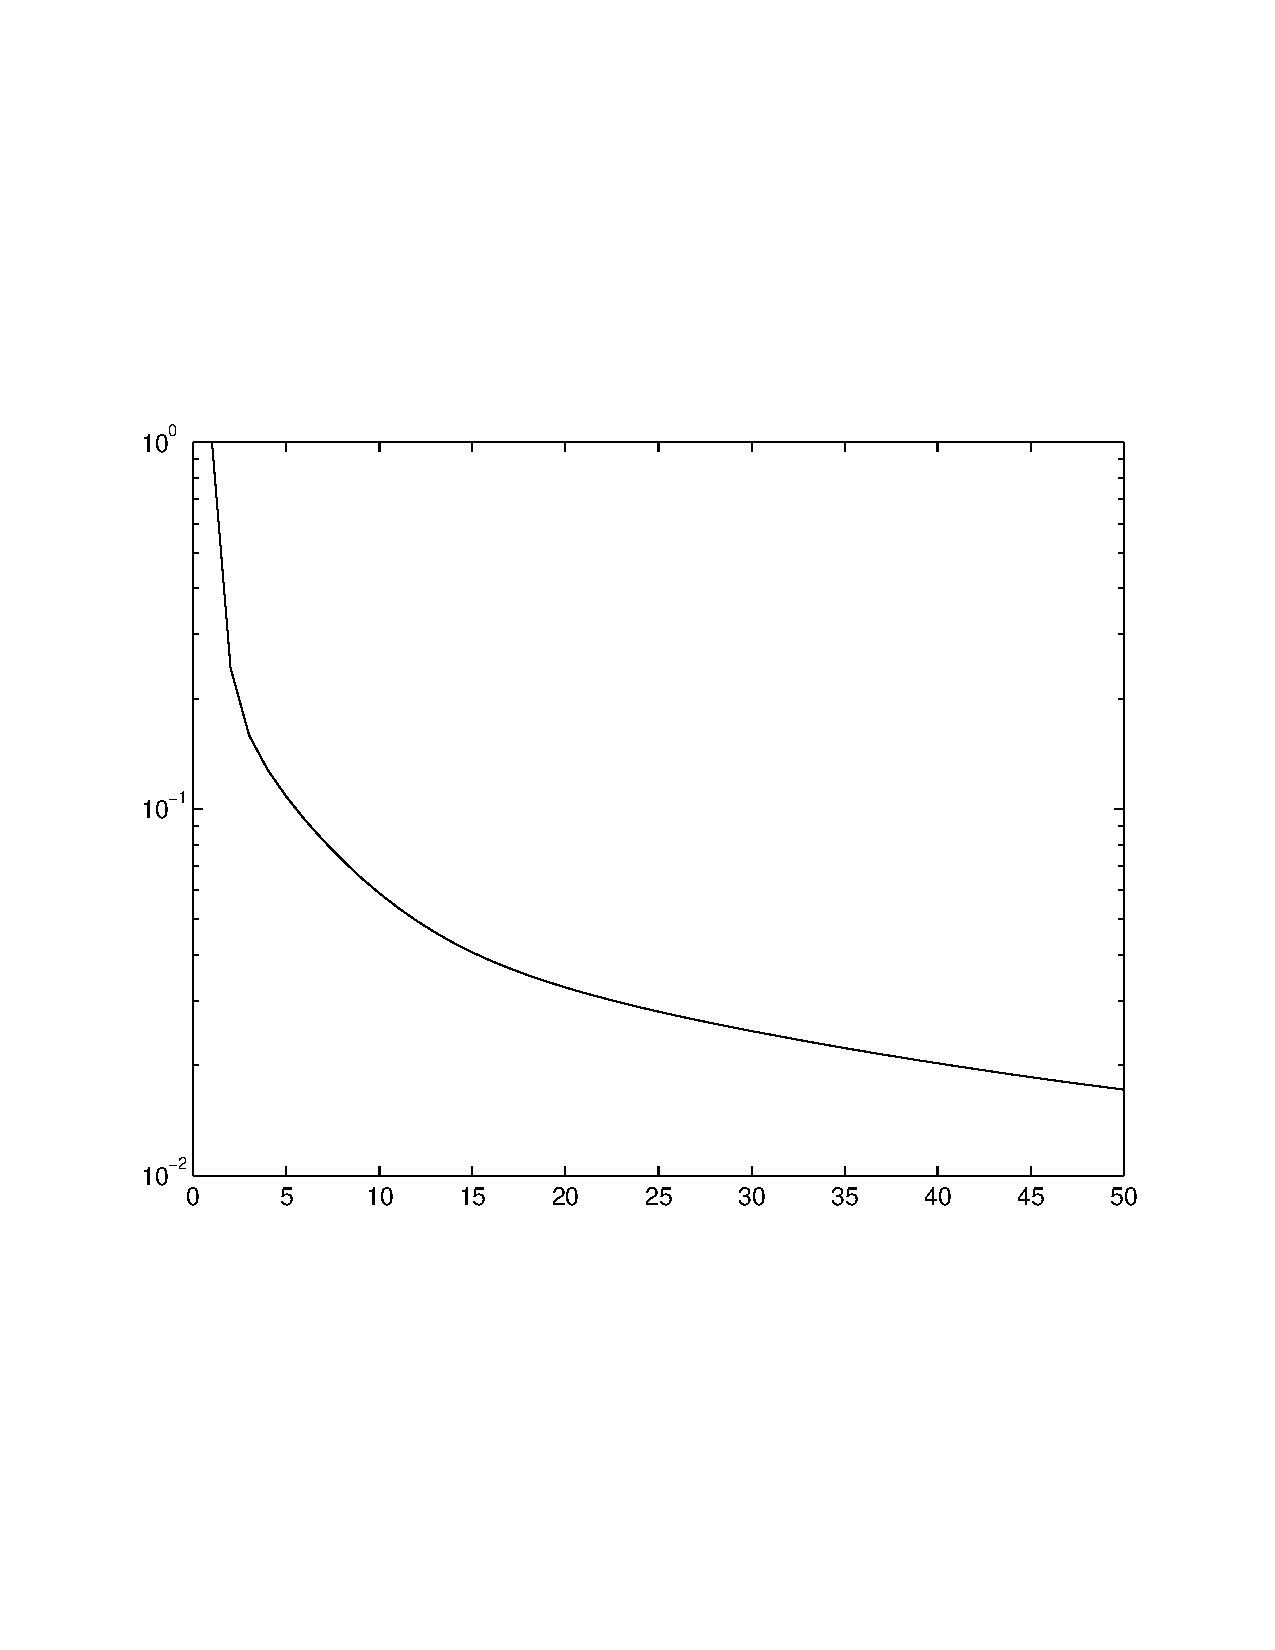
\includegraphics[height=5cm,width=3in]{pictures/richardson.pdf}
\end{center}
\caption{A picture on the GD method convergence history
\label{fig:richardson}}
\end{figure}

Our main goal is to find a way to speed up such kind of rather slowly
convergent iterative scheme.  To do that, we need to study its
convergent property in more microscopic level.  First of all, let us
now take a careful look at the convergence history picture and make
the following observation:
\begin{quote}
\underbar{\it Observation 1.}  The scheme converges rather fast in the
very beginning but then slows down after a few steps. Overall, the method 
converges very slowly. 
\end{quote}
To further understand this phenomenon, let us plot the detailed
pictures of the error functions in the first few iterations.
After a careful look at these pictures, we have the following 
observation:
\begin{quote}
\underbar{\it Observation 2.} The scheme not only converges fast in the
first few steps, but also smooth out the error function very quickly.
\end{quote}

\begin{figure}[!htb]
\begin{center}
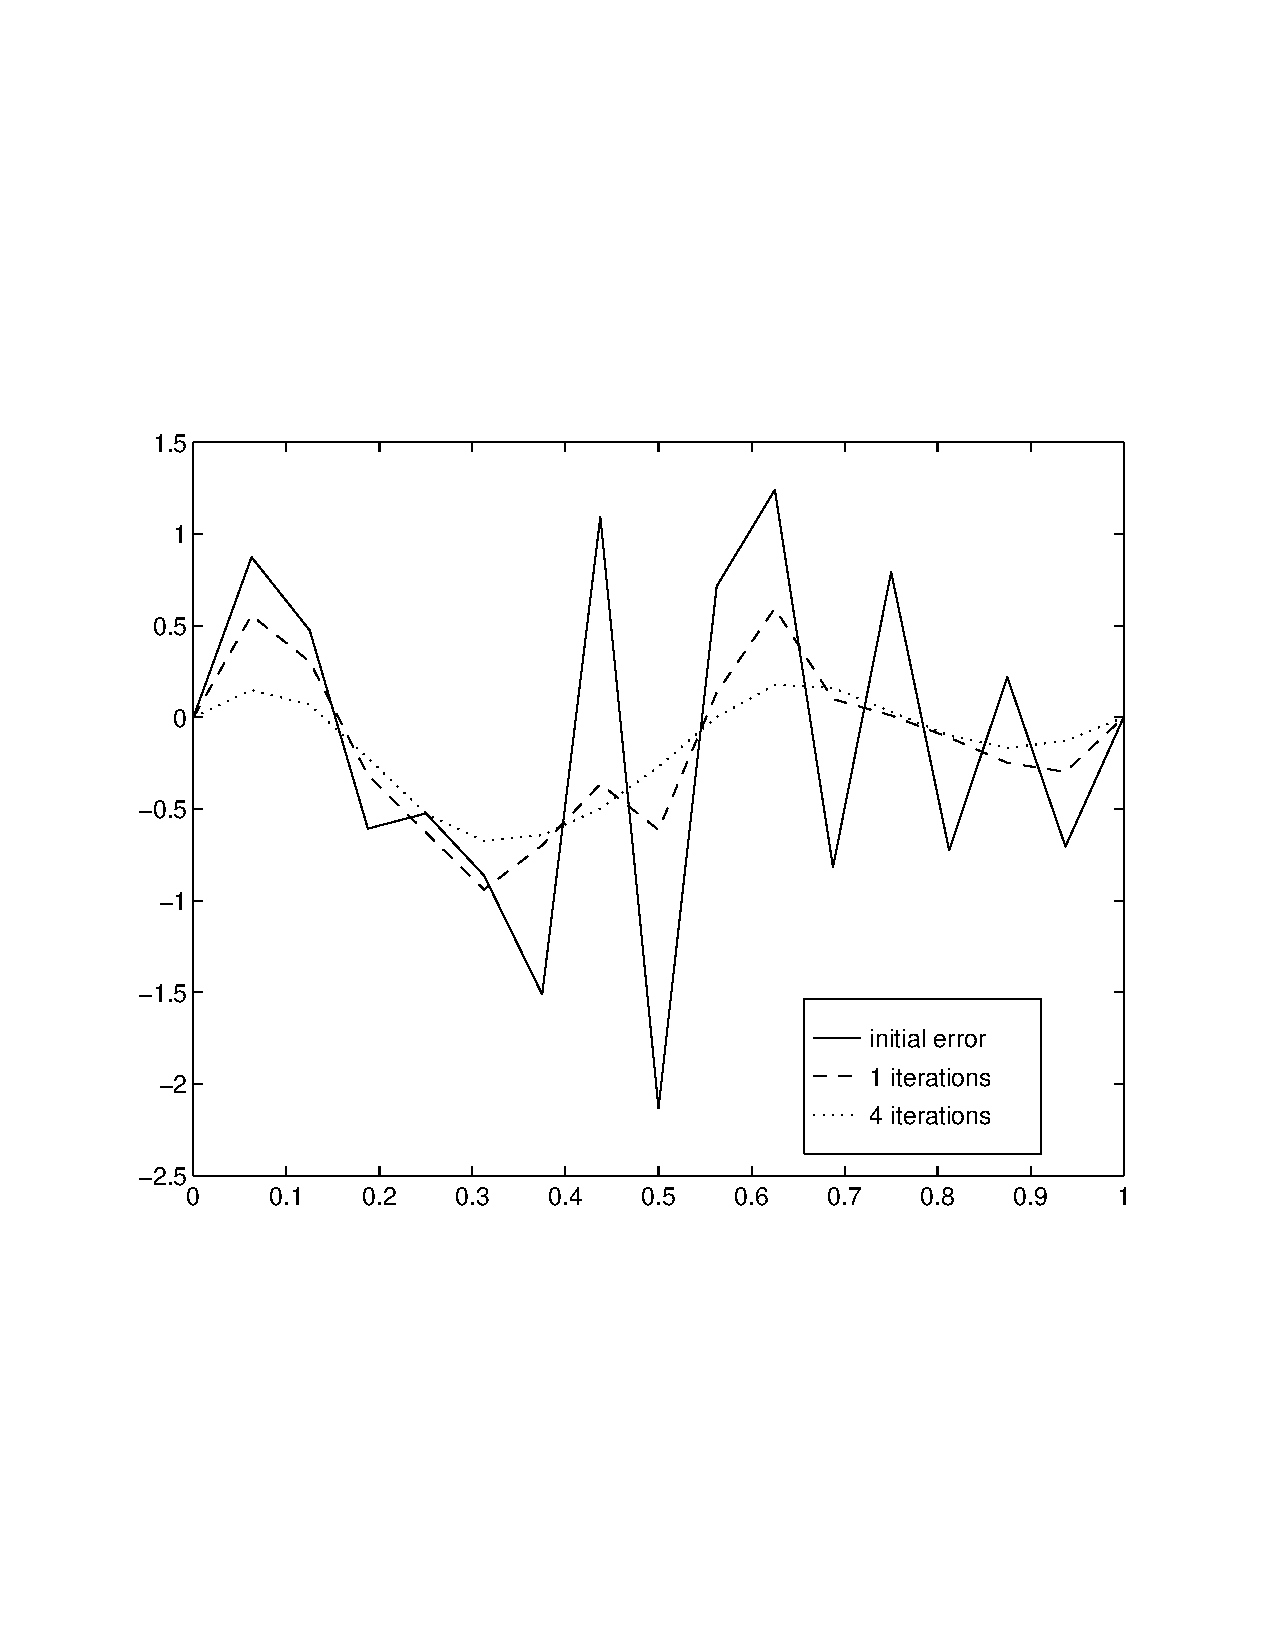
\includegraphics[height=5cm,width=3in]{pictures/smoothing.pdf}
\end{center}
\caption{The smoothing effect of the gradient descent method
\label{fig:smoothing}}
\end{figure}


In other words, the error function becomes a much smoother function
after a few such simple iterations.  This property of the iterative
scheme is naturally called {\it a smoothing property} and an iterative
scheme having this smoothing property is called a {\it smoother}.

The above two observations, especially the second one, concern the
most important property of the simple gradient descent method that we can
take advantage to get a much faster algorithm.


The gradient descent method can be written in terms of $S_{0}:\mathbb R^{N}\rightarrow \mathbb R^{N}$ satisfying
\begin{equation}
\label{jacobi1d}
\mu^{(1)}=(S_{0}b)={h\over 4} b,
\end{equation}
for equation \eqref{min} with initial guess zero.
If we apply this method twice, then
$$
\mu^{(2)}=S_1(b) = S_{0} b + S_0(b - A\ast(S_{0}b)),
$$
with element-wise form
\begin{equation} 
\begin{aligned}
\mu^{(2)}_{i} &={h\over 16}(b_{i-1}+6b_i+b_{i+1}).
\end{aligned}
\end{equation}
Then by the definition of convolution \eqref{con010}, we have
 \begin{equation}\label{eq:convS}
\mu^{(1)}= S_{0}\ast b \quad \mu^{(2)} = S_1 \ast b.
\end{equation}
with
\begin{equation}\label{eq:kernel-S1d}
S_{0} = {h\over 4},
\end{equation}
and 
\begin{equation}\label{eq:kernel-S2}
S_1={h\over 16}[1,6,1].
\end{equation} 

Hence we denote $S_0$ or $S_1$ as $S$.

Now for any given $\mu^{(0)}=\tilde{\mu}^{(0)}$, 
\begin{equation}
\begin{aligned}
&m=1,2,\cdots,2\nu\\
&\mu^{(m)}=\mu^{(m-1)}+S_0\ast(b-A\ast\mu^{(m-1)})
\end{aligned}
\end{equation}
$$\Leftrightarrow$$
\begin{equation}
\begin{aligned}
&m=1,2,\cdots,\nu\\
&\tilde{\mu}^{(m)}=\tilde{\mu}^{(m-1)}+S_1\ast(b-A\ast\tilde{\mu}^{(m-1)})
\end{aligned}
\end{equation}
we obtain $\mu^{(2\nu)}=\tilde{\mu}^{(\nu)}$ which means one step $S_1$ is equivalent to two steps of $S_0$.

\paragraph{Convergence and smoothing properties of GD}
Because of the extraordinary importance of this smoothing property, we
shall now try to give some simple theoretical analysis.  To do this,
we make use of the eigenvalues and eigenvectors of the matrix $A$.
\paragraph{Fourier analysis for the gradient descent method}
Our earlier numerical experiments indicate that the gradient descent
method has a smoothing property.  Based on our understanding of the
relation between the smoothness and the size of Fourier coefficients,
we can imagine that this smoothing property can be analyzed using the
discrete Fourier expansion.

Let $\mu$ be the exact solution of \eqref{min} and $\mu^{(m)}$ the result of
$m-th$ iteration from the gradient descent method \rf{1dRichardson}.  Then
$$
\mu-\mu^{(m)}=(1-\eta A\ast)(\mu-\mu^{(m-1)})=\ldots=(1-\eta A\ast)^m(\mu-\mu^{(0)}).
$$
Consider the Fourier expansion of the initial error:
$$
        \mu-\mu^{(0)}=\sum_{k=1}^N\alpha_k\xi^k.
$$
Then 
$$
        \mu-\mu^{(m)}=\sum_{k=1}^N\alpha_k(I-\eta A\ast)^m\xi^k.
$$
Note that $\eta=h/4$ and for any polynomial $p$
$$
p(A\ast)\xi^k=p(\lambda_k)\xi^k,
$$
we get
$$
        \mu-\mu^{(m)}=\sum_{k=1}^N\alpha_k(1-\eta\lambda_k)^m\xi^k
        =\sum_{k=1}^N\alpha_k^{(m)}\xi^k
$$
where 
$$
\alpha_k^{(m)}=\bigg(1-\sin^2{{k\pi}\over {2(N+1)}}\bigg)^m\alpha_k.
$$
For $k$ close to $N$, for example $k=N$,
note that 
$$
1-\sin^2{{N\pi}\over {2(N+1)}}=\cos^2{{N\pi}\over {2(N+1)}}
=\sin^2({\pi\over2}-{{N\pi}\over {2(N+1)}})
$$
implies
$$
|\alpha_N^{(m)}|=|\alpha_N|\sin^{2m}{{N+1-N}\over{N+1}}{\pi\over 2}
\le |\alpha_k|\bigg({{1}\over{N+1}}{\pi\over 2}\bigg)^{2m}
$$
which approaches to $0$ very rapidly when
$m\rightarrow\infty$. This means that high frequency components get
damped very quickly. 

However, for $k$ far away from $N$, for example $k=1$, note that
$$
\sin^2{{\pi}\over {2(N+1)}}\le \left({{\pi}\over {2(N+1)}}\right)^2
$$
implies
$$
|\alpha_1^{(m)}|= |\alpha_1| \bigg(1-\sin^2{{\pi}\over {2(N+1)}}\bigg)^m\ge  |\alpha_1|  \left(1-\left({{\pi}\over {2(N+1)}}\right)^2\right)^m
$$
which approaches to $0$ very slowly when
$m\rightarrow\infty$. 

This simple analysis clearly justifies the smoothing property that has
been observed by numerical experiments.

%\newpage

\begin{figure}[!ht]
\setlength{\abovecaptionskip}{0pt}
\setlength{\belowcaptionskip}{0pt}
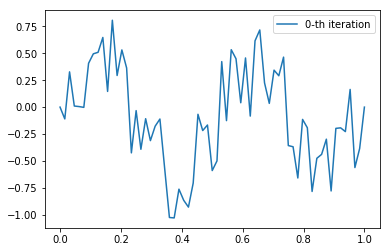
\includegraphics[width=5cm]{figures/jianhongu0.png}\qquad
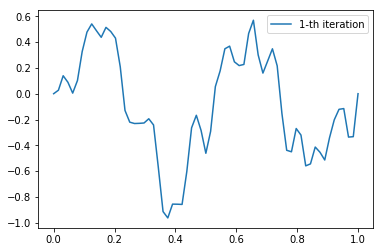
\includegraphics[width=5cm]{figures/jianhongu1.png}\qquad
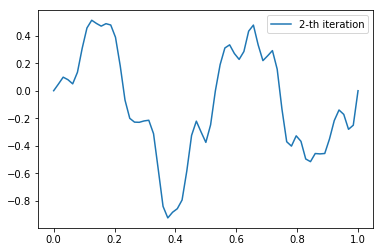
\includegraphics[width=5cm]{figures/jianhongu2.png}\qquad
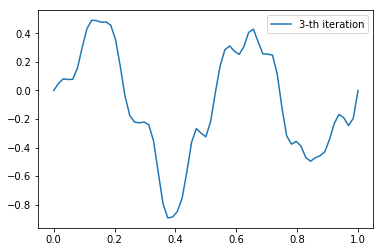
\includegraphics[width=5cm]{figures/jianhongu3.png}\qquad
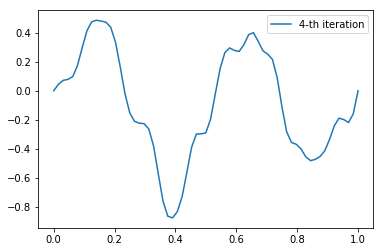
\includegraphics[width=5cm]{figures/jianhongu4.png}\qquad
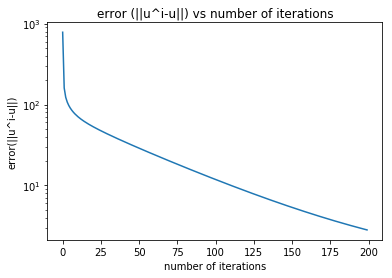
\includegraphics[width=5cm]{figures/jianhongGDerror.png}
\caption{\footnotesize{ $u-u^0$, $u-u^1$, $u-u^2$, $u-u^3$, $u-u^4$}}
\label{fig:Hmesh}
\end{figure}

%\begin{figure}[!ht] 
%\centering
%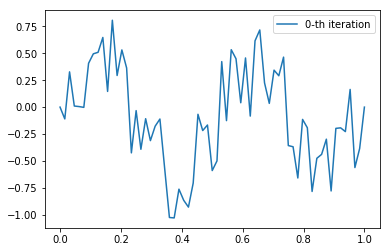
\includegraphics[width=5cm,height=4cm]{figures/jianhongu0.png}
%\caption{ $u^0$}
%\label{fig:u0j}
%\end{figure}
%\begin{figure}[!ht] 
%\centering
%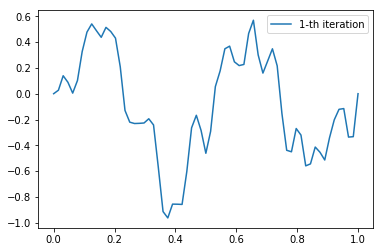
\includegraphics[width=5cm,height=4cm]{figures/jianhongu1.png}
%\caption{ $u^1$}
%\label{fig:u1j}
%\end{figure}
%\begin{figure}[!ht] 
%\centering
%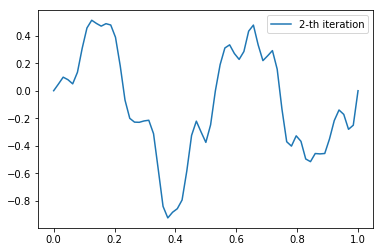
\includegraphics[width=10cm,height=8cm]{figures/jianhongu2.png}
%\caption{ $u^2$}
%\label{fig:u2j}
%\end{figure}
%\begin{figure}[!ht] 
%\centering
%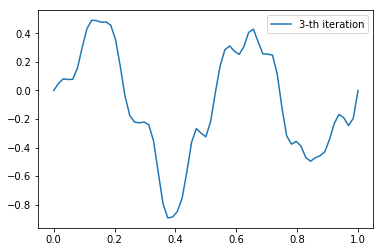
\includegraphics[width=10cm,height=8cm]{figures/jianhongu3.png}
%\caption{ $u^3$}
%\label{fig:u3j}
%\end{figure}
%\begin{figure}[!ht] 
%\centering
%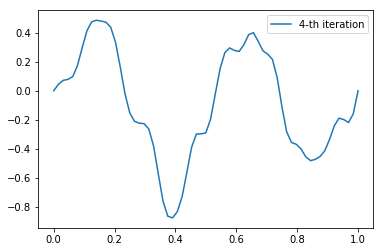
\includegraphics[width=10cm,height=8cm]{figures/jianhongu4.png}
%\caption{ $u^4$}
%\label{fig:u4j}
%\end{figure} 

\paragraph{An intuitive discussion} 
The gradient descent method is oftentimes called {\it local relaxation}
methods. This name refers to the fact that what that
algorithm does is just trying to correct the residual vector locally
at one nodal point at a time (recall that $\mu_j\approx u(x_j)$).
This local relaxation procedure is then effective to the error
components that are local in nature.  Incidentally, the nonsmooth or
high frequency component which oscillates across one or few grid
points have a strong local feature.  Therefore, it is not surprising the
 gradient descent  iteration can damp out these
nonsmooth components more easily.  This method is very inefficient
for relatively smoother components in the error since a smoother
function is more globally related in nature.


%\section{Multigrid algorithms}
%\subsection{Coarse grid correction and two grid method}
%\vspace{-1.8cm}
\begin{figure}[hpt]
\begin{center}
\includegraphics*[width=3in]{figures/twogrid.pdf}
%\vspace{-1.5cm}
\caption{Two level grids.} 
\label{Interpolation}
\end{center}
\end{figure} 

\begin{figure}[!htb]
\begin{center}
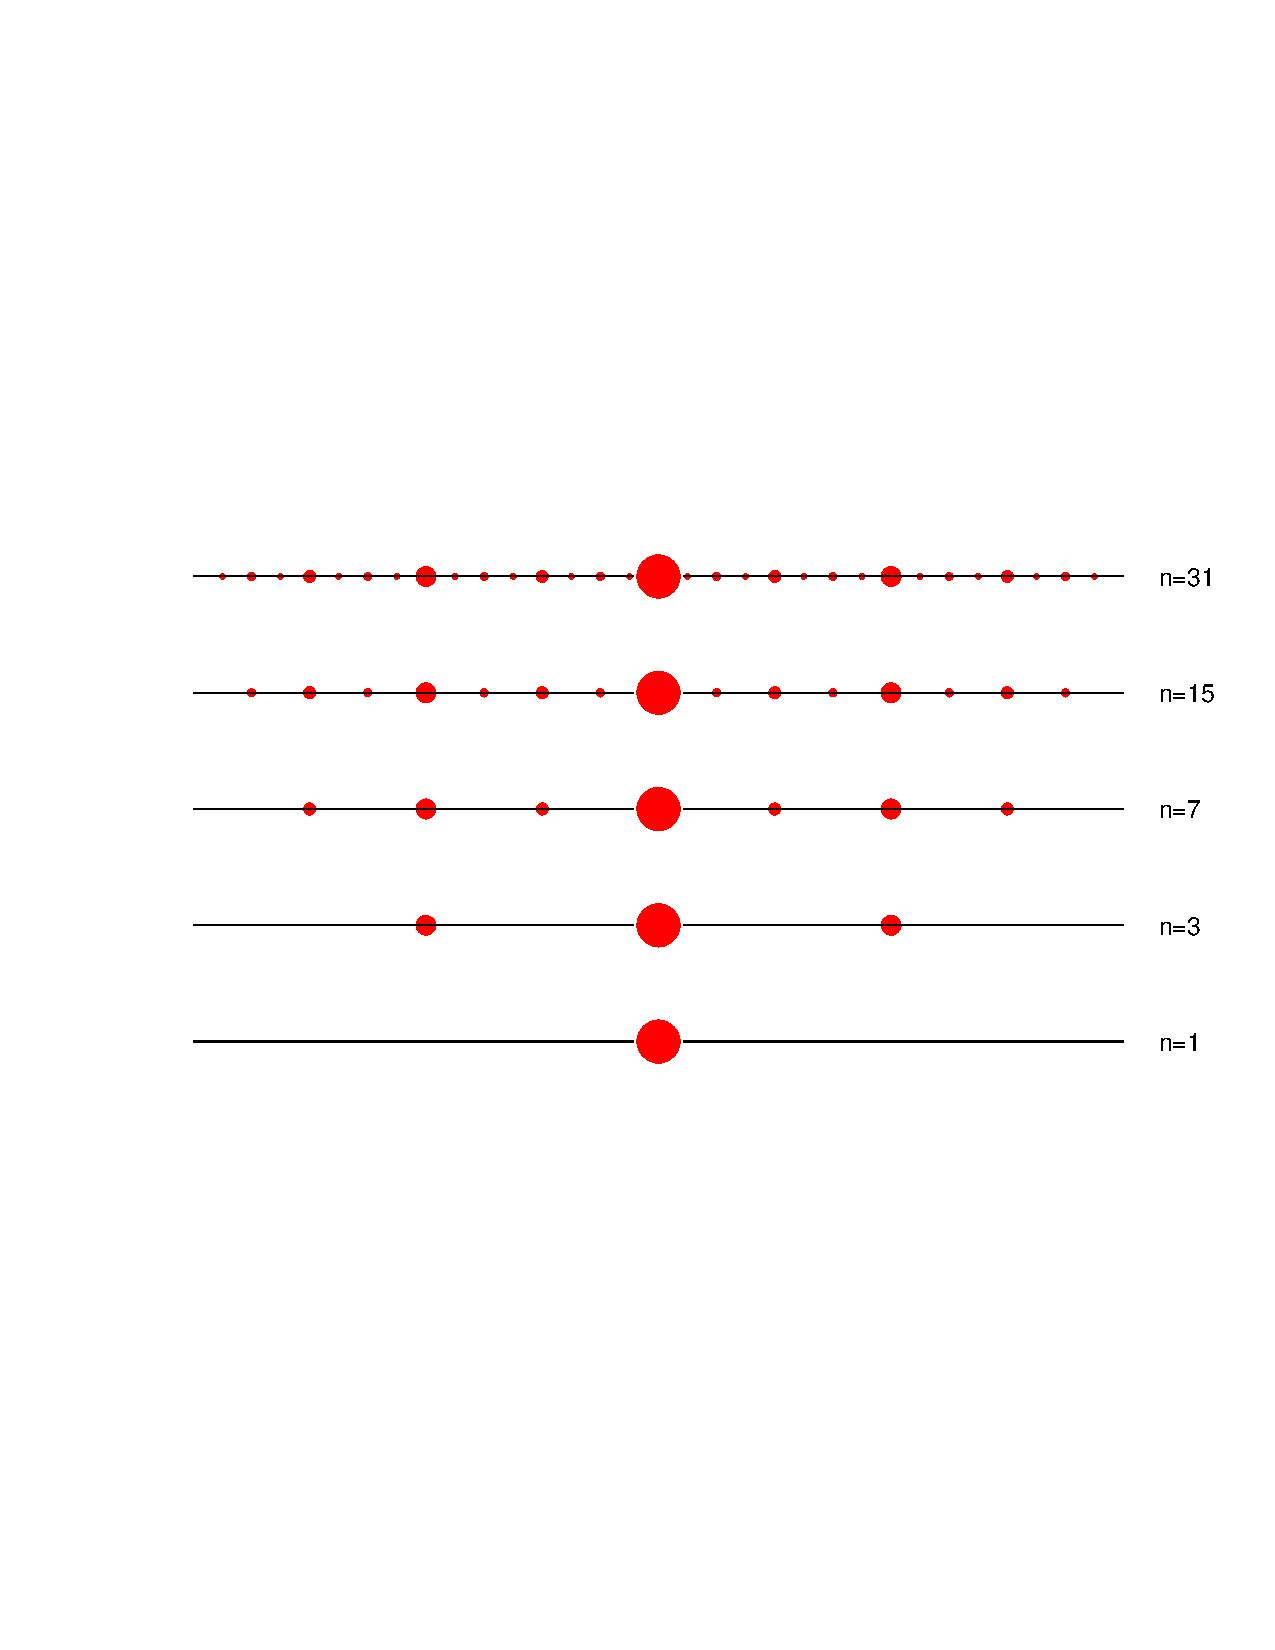
\includegraphics[width=3in]{pictures/manygr.pdf}
\end{center}
\caption{Multiple grids in one dimension
\label{fig:manygrids}}
\end{figure}

%\vspace{-0.2cm}
As we discussed earlier, although gradient descent iteration usually
converges very slowly, it does quickly smooth out the rough 
component in the error. In other words, the error becomes smooth 
after a few gradient descent iterations on a fine grid, but looks 
rough when viewed on a coarser grid. Hence, a few gradient descent
iterations can further reduce the error on the coarse grid. 
The main idea of two grid method or multigrid method is 
to use the fact that a smooth function can be well 
approximated on a coarser grid.  

In summery, we can write the two grid method in terms of finite element (FE) functions as follows:
\begin{algorithm}\caption{A two grid method (in terms of FE functions)}\Label{alg:2grid:opezero}
Input $u^0$.
\begin{enumerate}
\item [{\bf Step 1:}] Apply $\nu_1$-times gradient descent iterations for 
$$
\min_{v^1\in V_1} J(v^1)
$$
with initial guess $u^0$ to obtain $u^1\in V_1$.
\item [{\bf Step 2:}]  Apply $\nu_2$-times gradient descent iterations for 
$$
\min_{v^2\in V_2} J(u^1+v^2)
$$
with zero initial guess to obtain $u^2\in V_2$.
\item [{\bf Step 3:}]  Update: $u=u^1+u^2$.
%\item [{\bf Step 4:}]  Stop if converge or $u^0\update u$ and continue from step 1.
\end{enumerate}
\end{algorithm}
 
\newpage

\subsubsection{Realization of step 1:} 
\smallskip\hrule \smallskip 

Step 1: Given $u^{1,0}\in V_1$, apply $\nu_1$-times gradient descent method for 
$$
\min_{v^1\in V_1} J(v^1)
$$
with initial guess $u^{1,0}$ to obtain $u^1\in V_1$.
\smallskip\hrule \smallskip 


Let $\displaystyle u^{1,0}=\sum_{i=1}^{n_1}\mu^0_i\phi_i^1,\quad v^1=\sum_{i=1}^{n_1}\nu^1_i\phi_i^1,\quad  \mu^0=\{\mu^0_i\}^{n_1}_{i=1},\quad  \nu^1=\{\nu^1_i\}^{n_1}_{i=1}$,

where $\phi^1=(\phi^1_1,\phi^1_2,\cdots,\phi^1_{n_1})$
is the nodal basis of $V_1$. 

Namely, $b^1=b, \mu^1\leftarrow \mu^0$,  for $i=1:\nu_2$ 
$$
\mu^1\leftarrow  \mu^1-\eta_1 (A_1\ast \mu^1-b^1).
$$
After $\nu_1$ iterations, we obtain updated $\mu^1$ and $\displaystyle  u^1=\sum_{i=1}^{n_1}\mu^1_i\phi_i^1$.

\subsubsection{Realization of step 2:} 
\smallskip\hrule \smallskip 
{\bf Step 2:}   Apply $\nu_2$-times gradient descent iterations for 
$$
\min_{v^2\in V_2} J(u^1+v^2)
$$
with zero initial guess to obtain $u^2\in V_2$. 
\smallskip\hrule \smallskip  
Let 
$$
u^1=\sum_{i=1}^{n_1}\mu^1_i\phi_i^1,~v^2=\sum_{i}^{n_2}\nu^2_{i}\phi^{2}_i,~\mu^1=\{\mu^1_i\}^{n_1}_{i=1}, ~ \nu^2=\{\nu^2_{i}\}^{n_2}_{i=1}.$$
We have
\begin{equation}\label{min2h} 
\begin{aligned}
J(u^1+v^2)&=\frac12\int_0^1|(u^1+v^2)'|^2dx-\int_0^1f(u^1+v^2)dx\\
&=J(u^1)+J(v^2)+\int_0^1(u^1)'(v^2)'dx\\
&=\frac12 (\mu^1)^TA_1\ast \mu^1+\frac12 (\nu^2)^TA_2\ast\nu^2-(\nu^2)^Tr^2
\end{aligned}
\end{equation}
where 
\begin{equation}
r_i^2=\int_0^1 f\phi^2_i -(u^1)'(\phi^2_i)'dx=(f,\phi^2_i)-a(u^1,\phi^2_i).
\end{equation}

Now noting that 
\begin{equation}\label{prolongation}
\phi^2_i=\frac12 \phi^1_{2i-1}+ \phi^1_{2i} +\frac12 \phi^1_{2i+1},
\end{equation}
Let $\phi^2=\{\phi^2_i\}_{i=1}^{n_2}, \phi^1=\{\phi^1_i\}_{i=1}^{n_1}$. 
Using the convolution with stride notation,  we obtain 
\begin{equation}\label{rescon}
\phi^2=R\ast_2\phi^1
\end{equation}
with $R=[\frac12,1,\frac12]$.
Furthermore, 
\begin{equation}
\begin{aligned}
r^2_i&=(f, \frac12 \phi^1_{2i-1}+ \phi^1_{2i} +\frac12 \phi^1_{2i+1})-a(u^1,  \frac12 \phi^1_{2i-1}+ \phi^1_{2i} +\frac12 \phi^1_{2i+1})\\
&\displaystyle= \frac12 b^1_{2i-1}+ b^1_{2i} +\frac12 b^1_{2i+1}- \Big(\frac12 (A_1\ast\mu^1)_{2i-1}+   (A_1\ast\mu^1)_{2i}+ \frac12(A_1\ast\mu^1)_{2i+1}\Big)\\
&\displaystyle= \frac12 (b^1-A_1\ast\mu^1)_{2i-1}+ (b^1-A_1\ast\mu^1)_{2i}+\frac12 (b^1-A_1\ast\mu^1)_{2i+1}\\
&\displaystyle= \frac12 r^1_{2i-1}+ r^1_{2i} +\frac12 r^1_{2i+1},
\end{aligned}
\end{equation}
where $r^1=b^1-A_1\ast\mu^1$.
\begin{lemma}
Using the convolution with stride notation, we have $$r^2=R\ast_2r^1$$ with $R=[\frac12,1,\frac12]$.
\end{lemma}
Therefore applying gradient descent method $\nu_2$-times for \eqref{min2h} reads: 

$r^1=b^1-A_1\ast\mu^1, r^2=R\ast_2r^1, \mu^2\leftarrow 0$,
for $i=1:\nu_2 $ 
\begin{equation}
\mu^2\leftarrow \mu^2-\eta_2(A_2\ast \mu^2-r^2). 
\end{equation}
After $\nu_2$ iterations, we obtain updated $\mu^2$ and $\displaystyle  u^2=\sum_{i=1}^{n_2}\mu^2_{i}\phi_i^2$.

\subsubsection{Realization of step 3:} 
\smallskip\hrule \smallskip 
{\bf Step 3:}  $u=u^1+u^2$. 
\smallskip\hrule \smallskip 

Let $\displaystyle  \mu^2=\{\mu^2_{i}\}^{n_2}_{i=1}, \phi^{2}=\{\phi^2_i\}^{n_2}_{i=1}$.
Therefore  $u^2=\sum\limits_{i=1}^{n_2}\mu^2_{i}\phi^2_i
=(\mu^2, \phi^2)_{l^2}$ and by \eqref{rescon} we have
\begin{equation}
\begin{split}
u^2&=(\mu^2, \phi^2)_{l^2}=(\mu^2, R\ast_2\phi^1)_{l^2}=(R\ast_2^{\top}  \mu^2,  \phi^1)_{l^2}\\
&=\sum_{i=1}^{n_1}\left(R\ast_2^{\top} \mu^2\right)_i \phi^1_i
\end{split}
\end{equation}
with $R=[\frac 12,1,\frac12]$.
\begin{lemma}
The prolongation can be written as 
$R\ast_2^T: \mathbb R^{n_2}\rightarrow \mathbb R^{n_1}$, for $\mu^2\in \mathbb R^{n_2}, (R\ast_2^T \mu^2)\in R^{n_1}$ with
$$
(R\ast_2^T \mu^2)_{2i}=\mu^2_i\quad (R\ast_2^T \mu^2)_{2i+1}=\frac 12 (\mu^2_{i+1} +\mu^2_{i}).
$$
\end{lemma}
Noting that $\displaystyle u^1=\sum_{i=1}^{n_1}\mu^1_i\phi_i^1,~\mu^1=\{\mu^1_i\}^{n_1}_{i=1}$, we obtain 
$$
\mu=\mu^1+R\ast_2^T \mu^2\quad\hbox{and}\quad u=u^1+u^2.
$$
%\newpage
Next we show how to realize the Algorithm \ref{alg:2grid:opezero} in vector and convolution form.
%\begin{algorithm}\caption{A two grid method
%$\mu = {\text{2G1}}(b; \mu^0; 2,\nu_1, \nu_2)$}
%\Label{alg:2grid:opecoze}
%Given $\mu^0$.
%\begin{enumerate}
%\item[{\bf Step1:}] 
%
%Set $b^1=b, \mu^1\leftarrow\mu^0$. 
%
%{\bf For} $i=1:\nu_1$ 
%$$
%\mu^1\leftarrow  \mu^1-\eta_1 (A_1\ast \mu^1-b^1).
%$$
%{\bf end for}
%\item [\bf{Step 2:}] Set $r^1=b^1-A_1\ast\mu^1, r^2=R\ast_2r^1,
%  \mu^2\leftarrow 0$. 
%
%{\bf For} $i=1:\nu_2 $ 
%\begin{equation}
%\mu^2\leftarrow \mu^2-\eta_2(A_2\ast \mu^2-r^2). 
%\end{equation}
%{\bf end for}
%\item [{\bf Step 3:}] Update: $\mu=\mu^1+R\ast_2^T \mu^2$.
%\end{enumerate}
%\end{algorithm}

\begin{breakablealgorithm}%[!htb]
	\caption{A two grid algorithm $\mu = {\text{2G1}}(b; \mu^0; 2,\nu_1, \nu_2)$}
\label{alg:L-Slash11d}
\begin{algorithmic}
%	 \State 
%		$$
%		u \leftarrow u^0.
%		$$
	\State Set up
		$$
		b^1 = b, \quad \mu^{1}=\mu^0. 
		$$
		\State Step 1: Smoothing and restriction from fine to coarse level (nested)
		\For{$i = 1:\nu_1$}
		\State
		\begin{equation}\label{eq:smoothing}
		\mu^{1} \leftarrow \mu^{1} + S^1 \ast (b^1 - A_1 \ast \mu^1).
		\end{equation}
		\EndFor
		\State Step 2: Form restricted residual and set initial guess:
		$$
		\mu^{2} \leftarrow 0, \quad b^{2} \leftarrow R \ast_2
                (b^1-  A_1\ast \mu^{1}), 
%A_{2} = R\ast_2 A_1 \ast (R\ast_2^\top).
		$$
		\For{$i = 1:\nu_2$}
		\State
		\begin{equation}\label{eq:smoothing}
		\mu^2 \leftarrow \mu^2+ S^2 \ast (b^2- A_2\ast \mu^2).
		\end{equation}
		\EndFor
		\State Step 3: Prolongation and restriction from coarse to fine level
		\State
		$$
		\mu^{1} \leftarrow \mu^{1} + R  \ast_2^{\top} \mu^{2}.
		$$
		\State
		$$
		\mu \leftarrow \mu^{1}.
		$$
	\end{algorithmic}
\end{breakablealgorithm}






%\subsection{Multilevel coarse grid corrections and a multigrid method}
\Label{sc:mg-fd}
To describe a multigrid algorithm, we first need to have a multiple
level of grids, say $\mathcal T_\ell$ with $\ell=1:J$ and $\mathcal T_1=\mathcal T_h$ being the
finest mesh.  There are many ways to obtain multiple level of grids
and one simple definition of the grid points in $\mathcal T_\ell$ is as follows:
$$
        x_i^\ell=\frac{i}{2^{J+1-\ell}},\quad i=1,2,\cdots, N_\ell, \ell=1,2,\cdots,J,
$$
where $N_\ell=2^{J+1-\ell}-1$.  Note that $\mathcal T_{\ell-1}$ can be viewed as being obtained
by adding midpoints of the subintervals in ${\mathcal T}_{\ell}$.  For each $\ell$
the set of above nodes will be denoted by $\mathcal N_\ell$.

\begin{figure}[!htb]
\begin{center}
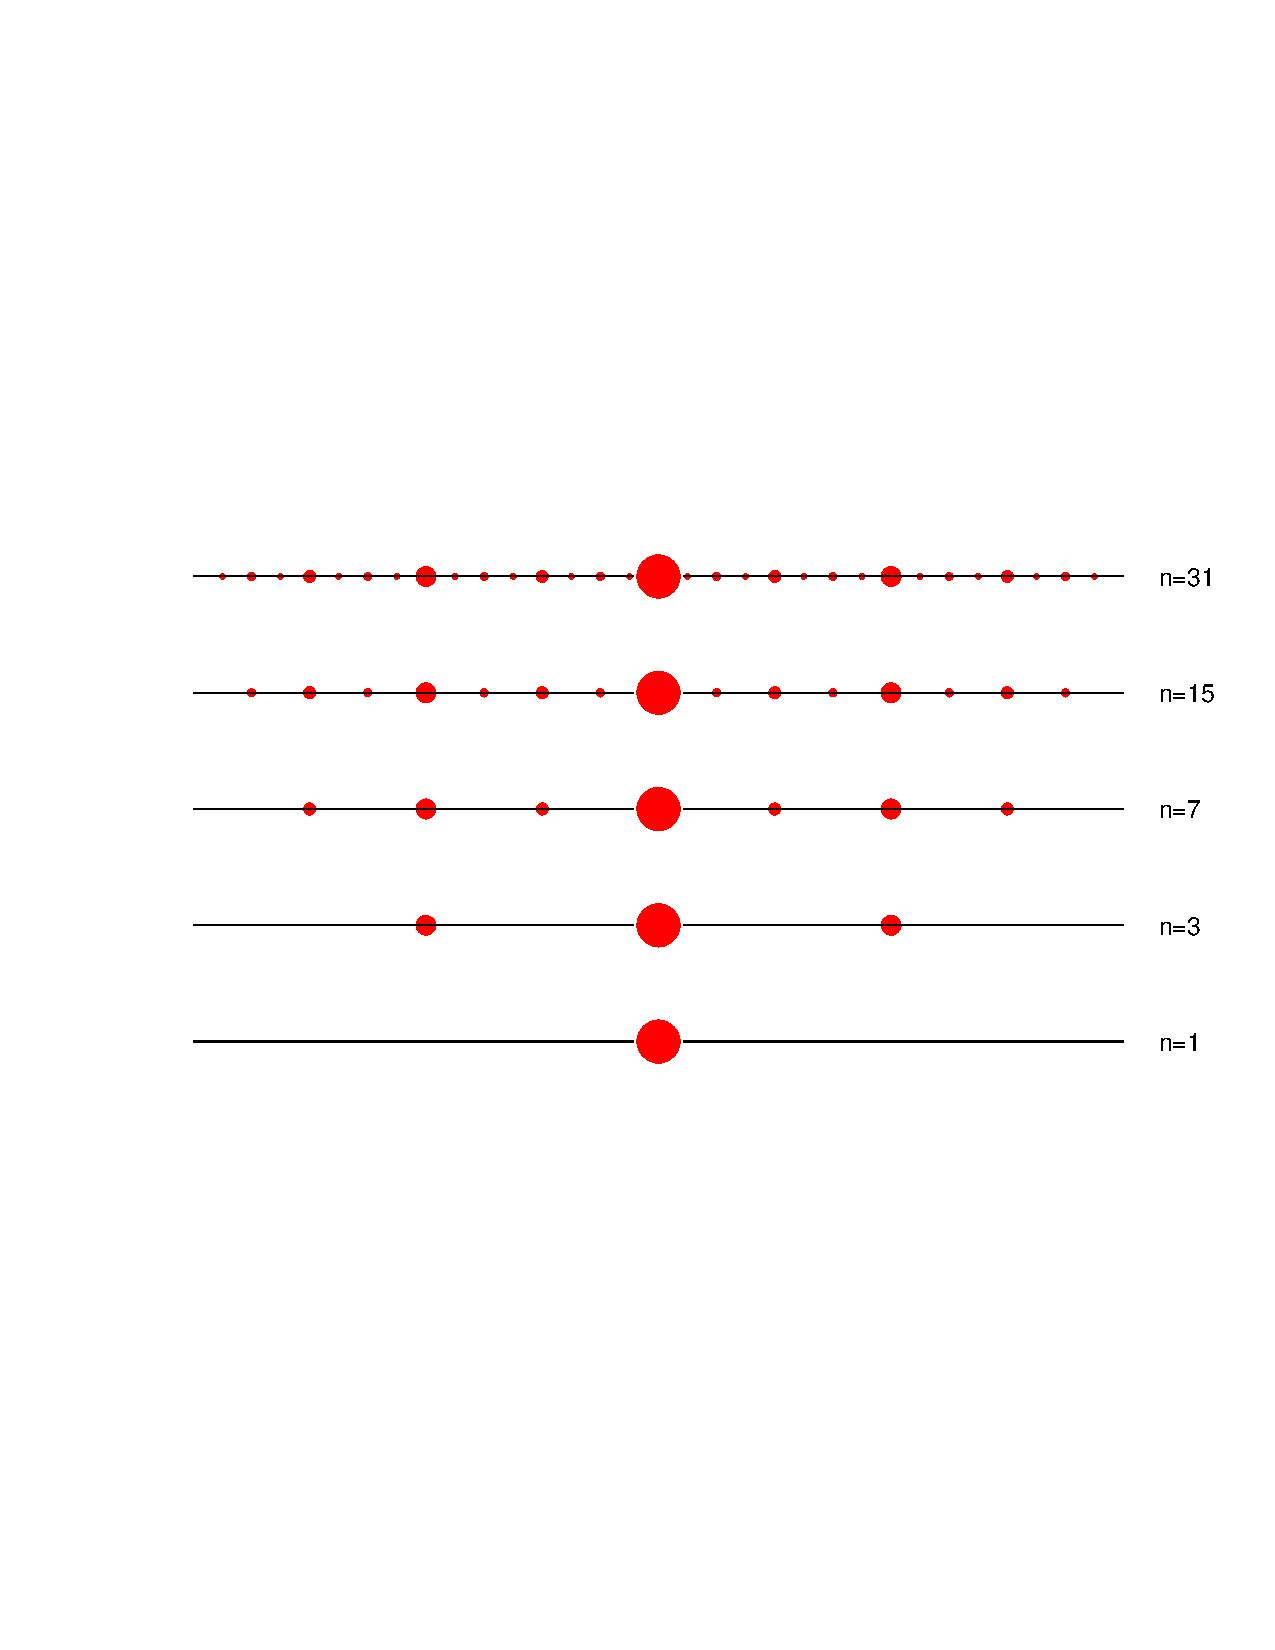
\includegraphics[width=3in]{pictures/manygr.pdf}
\end{center}
\caption{Multiple grids in one dimension
\label{fig:manygrids}}
\end{figure}


With our previous experiences in two-grid method, the description of a
multigrid method is not very difficult.  In fact, the multiple level
grids are treated by treating each two consecutive grids, say $\mathcal T_{\ell-1}$
versus $\mathcal T_{\ell}$.  If we think $\mathcal T_{\ell-1}$ versus $\mathcal T_{\ell}$ like
$\mathcal T_h$ and $\mathcal T_{2h}$, then there is not much new in the multigrid
setting.


Let us give some on details the definition of the restriction and
prolongation matrices.  The restriction matrix $R_{\ell-1}^\ell: R^{N_{\ell-1}}
\mapsto R^{N_{\ell}}$ can be defined by
\begin{equation}\Label{restrictk}
\gamma^{\ell}=R_{\ell-1}^\ell\gamma^{\ell-1}: \;
\gamma^{\ell}_i={1\over2}\gamma^{\ell-1}_{2i-1}+\gamma^{\ell-1}_{2i}+{1\over2}\gamma^{\ell-1}_{2i+1}.
\end{equation}
In matrix form 
\begin{equation}
\label{1drestriction}
R_{\ell-1}^\ell=\left(
\begin{array}{ccccccccc}
\frac{1}{2}& 1&\frac{1}{2}&&&&&&\\
&&\frac{1}{2}&1&\frac{1}{2}&&&&\\
&&&&\frac{1}{2}&1&\frac{1}{2}&&\\
&&&&&&\ddots&&\\
&&&&&&\frac{1}{2}&1&\frac{1}{2}\\
\end{array}
\right)
\end{equation}
For a special case, when $N_1=7, N_2=3$, we have 
\begin{equation}
\label{1drestriction3}
R_1^2=\left(
\begin{array}{ccccccc}
\frac{1}{2}& 1&\frac{1}{2}&0&0&0&0\\
0&0&\frac{1}{2}&1&\frac{1}{2}&0&0\\
0&0&0&0&\frac{1}{2}&1&\frac{1}{2}\\
\end{array}
\right).
\end{equation}




The prolongation matrix
$P_{\ell}^{\ell-1}: R^{N_{\ell}}
\mapsto R^{N_{\ell-1}}$ can be defined as 
\begin{equation}\Label{prolongk}
~~\epsilon^{\ell-1}=P^{\ell-1}_{\ell}\epsilon^{\ell}: \; \epsilon^{\ell-1}_{2i}=\epsilon^{\ell}_i, \epsilon^{\ell-1}_{2i+1}
= {1\over~2}(\epsilon^{\ell}_i+\epsilon^{\ell}_{i+1}), \; i=1:N_{\ell}.
\end{equation}

With the restriction and prolongation matrices in hands, we can now
present a multilevel version of the earlier two-grid algorithm.  As
mentioned before, the idea is to repeat this two grid process for the
coarse grid by using an even coarser grid.  The resulting algorithm is
just a desired multigrid algorithm. 


Using the convolution with stride notation, the restriction subprocess can also be written as 
$R\ast_2: \mathbb R^{N_\ell}\rightarrow  \mathbb R^{N_{\ell+1}}$, for any $v\in \mathbb R^{N_\ell}, u=(R\ast_2 v)\in R^{N_{\ell+1}}$ with
$$
 (R\ast_2 v)_i=\frac 12 v_{2i-1} +v_{2i}+\frac 12 v_{2i+1},\quad  \mbox{namely}\quad R\ast_2v=R_{\ell-1}^\ell v
$$
where $R=[\frac 12,1,\frac12]$ and $R_{\ell-1}^\ell $ is defined by \eqref{1drestriction}.

Next 
let $u^{\ell+1}=\sum\limits_{j=1}^{n_{\ell+1}}\mu_{j}^{\ell+1}\phi^{\ell+1}_{j}
=(  \mu^{\ell+1}, \phi^{\ell+1})_{l^2}$, then we have
\begin{equation}
\begin{split}
u^{\ell+1}&=( \mu^{\ell+1}, \phi^{\ell+1})_{l^2}
=( \mu^{\ell+1}, R\ast_2\phi^{\ell})_{l^2}=(R\ast_2^{\top} \mu^{\ell+1}, \phi^{\ell})_{l^2}\\
&=\sum\limits_{j=1}^{n_{\ell}}\left(R\ast_2^{\top} \mu^{\ell+1}\right)_{j}\phi^{\ell}_{j}.
\end{split}
\end{equation}
The prolongation subprocess can be written as 
$R\ast_2^T: \mathbb R^{N_{\ell+1}}\rightarrow \mathbb R^{N_\ell}$, for any $v\in \mathbb R^{N_{\ell+1}}, u=(R\ast_2^T v)\in R^{N_\ell}$ with
$$
(R\ast_2^T v)_{2i}=v_i,\quad (R\ast_2^T v)_{2i+1}=\frac 12 (v_{i+1} +v_i),\quad  \mbox{namely}\quad R\ast_2^Tv=P^{\ell-1}_\ell v
$$
where $R=[\frac 12,1,\frac12]$.

Using the convolution notation, the subprocess to apply $A_\ell$ to 
a vector $v\in \mathbb R^{N_\ell}$ can be written as
$A_\ell\ast: \mathbb R^{N_\ell}\rightarrow \mathbb R^{N_\ell}$, for any $v\in \mathbb R^{N_\ell}, r=(A_\ell\ast v)\in R^{N_\ell}$ with
$$
(A_\ell\ast v)_{i}=\frac{1}{h_\ell}( -v_{i-1}+2v_i-v_{i+1})
$$
where $A_\ell=\frac{1}{h_\ell}[-1,2,-1]$.

\newpage

\begin{breakablealgorithm}%[!htb]
	\caption{A multigrid algorithm $\mu = {\text{MG1}}(b; \mu^0; J,\nu_1, \cdots, \nu_J)$}
\label{alg:L-Slash11dm}
\begin{algorithmic}
%	 \State 
%		$$
%		u \leftarrow u^0.
%		$$
	\State Set up
		$$
		b^1 = b, \quad \mu^{1}=\mu^0. 
		$$
		\State Smoothing and restriction from fine to coarse level (nested)
		\For{$\ell = 1:J$}
		\For{$i = 1:\nu_\ell$}
		\State
		\begin{equation}\label{eq:smoothing}
		\mu^{\ell} \leftarrow \mu^{\ell} + S^\ell \ast (b^\ell - A_\ell \ast \mu^{\ell}).
		\end{equation}
		\EndFor
		\State Form restricted residual and set initial guess:
		$$
		\mu^{\ell+1} \leftarrow 0, \quad b^{\ell+1} \leftarrow R \ast_2 (b^\ell -  A_\ell \ast \mu^{\ell}), A_{\ell+1} = R       \ast_2 A_\ell \ast (R\ast_2^\top).
		$$
		\EndFor
		\State Prolongation and restriction from coarse to fine level
		\For{$\ell = J-1:1$}
		\State
		$$
		\mu^{\ell} \leftarrow \mu^{\ell} + R  \ast_2^{\top} \mu^{\ell+1}.
		$$
%		%		\IF{V-cycle}
%		\For{$i = 1:\nu_\ell$}
%		\State
%		$$
%		u^{\ell,i} \leftarrow u^{\ell,i-1} + [B^{\ell,i}]^T (f^\ell - A^{\ell} u^{\ell,i-1})
%		$$
%		\EndFor
%		%		\ENDIF
		\EndFor
		\State
		$$
		\mu \leftarrow \mu^{1}.
		$$
	\end{algorithmic}
\end{breakablealgorithm}


Application of Multigrid:
		Given $\mu^{(0)}$, for $m=1,2,\cdots$ till convergence
		$$
		\mu^{(m)}= {\text{MG1}}(b; \mu^{{(m-1)}}; J,\nu_1, \cdots, \nu_J).
		$$
		
\example Let $f(x)=1$. Consider 
\begin{equation}\label{1Dposi}
\left\{
\begin{aligned}
-u''&= f, \,\, 0<x<1, \\
 u(0)&=u(1)=0.
\end{aligned}
\right.
\end{equation}
The true solution $u=\frac12 x(1-x)$. Given the partition with the grid points 
$x_i=\frac{i}{n+1}, i=0,1,\cdots,n+1$, then by finite element discretization, 
we obtain 
\begin{equation}\label{matrix}
A\ast \mu =b, A=\frac{1}{h}[-1,2,-1].
\end{equation}
Use gradient descent method and multigrid to solve \eqref{matrix} with random initial guess $\mu^0$.



\begin{figure}[!ht]
\centering
\setlength{\abovecaptionskip}{0pt}
\setlength{\belowcaptionskip}{0pt}
\includegraphics[width=8.3cm]{figures/mgcompare.png}
\caption{Comparison GD with Multigrid}
\label{fig:Hmesh}
\end{figure}






%\input{3FEM/1DMGvector}

%%%%%%%%%%%%%%%%%%%%%%%%%%%%%%%%%%
%
\section{Finite element method and convolution}\label{sec:mg}
Let us first briefly describe finite
element methods for the numerical solution of the following boundary
value problem
\begin{equation}
\label{laplace}
-\Delta u = f,  \mbox{ in } \Omega,\quad
u=0  \mbox{ on } \partial\Omega,\quad
\Omega=(0,1)^2.
\end{equation}
For the $x$ direction and the $y$ direction, we consider the partition:
\begin{equation}\label{partitionyx}
 0=x_0<x_1<\cdots<x_{n+1}=1, \quad x_i=\frac{i}{m+1},\quad (i=0,\cdots,m+1);
 \end{equation}
 \begin{equation}\label{partitiony}
 0=y_0<y_1<\cdots<y_{n+1}=1, \quad y_j=\frac{j}{n+1},\quad (j=0,\cdots,n+1).
\end{equation}
For $\Omega=(0,1)^2$, we just choose $m=n$. Such a uniform partition in the $x$ and $y$ directions leads us to a special example in two dimensions, a uniform square mesh $\R_h^2 = \big\{(ih,jh); i, j \in \Z\big\}$ (Figure \ref{fig:2dpartition}). 


\begin{figure}
\begin{center}
\setlength{\unitlength}{0.5mm}
\begin{picture}(45,45)(50,0)
\linethickness{0.25mm}
\multiput(0,0)(10,0){6}{\line(0,1){50}}
\multiput(0,0)(0,10){6}{\line(1,0){50}}
\put(0,0){\line(1,1){50}}
\put(10,0){\line(1,1){40}}
\put(20,0){\line(1,1){30}}
\put(30,0){\line(1,1){20}}
\put(40,0){\line(1,1){10}}
\put(0,10){\line(1,1){40}}
\put(0,20){\line(1,1){30}}
\put(0,30){\line(1,1){20}}
\put(0,40){\line(1,1){10}}
\put(47,34){$\displaystyle \left. \begin{array}{l}~ \\ ~\end{array}
\right\} h={1\over n+1}$}
\put(54,14){$\displaystyle N = n^2$}
\multiput(100,0)(10,0){6}{\line(0,1){50}}
\multiput(100,0)(0,10){6}{\line(1,0){50}}
\put(147,34){$\displaystyle \left. \begin{array}{l}~ \\ ~\end{array}
\right\} h={1\over n+1}$}
\put(154,14){$\displaystyle N = n^2$}
\end{picture}
\setlength{\unitlength}{0.5mm}
\end{center}
\label{fig:2dpartition}
\caption{Two-dimensional uniform grids for finite element}
\end{figure}

We consider two finite elements: continuous linear element and
bilinear element. These two finite element methods find $u_h\in V_h$
such that
\begin{equation}\label{Discrete:2d}
(\nabla u_h, \nabla v_h)=(f, v_h),\ \forall v_h\in V_h.
\end{equation}


Basis functions $\phi_{ij}$ satisfy 
\begin{equation}
  \label{NodalBasis}
\phi_{ij}(x_k,y_l)=\delta_{(i,j),(k,l)}.  
\end{equation}

Consider continuous linear finite element discretization of \eqref{laplace} on
the left triangulation in Fig \ref{fig:2dpartition}. The discrete
space for linear finite element is
$$
\mathcal V_h=\{v_h: v_h|_K\in P_1(K) \text{ and } v_h \text{ is globally continuous}\}.
$$ 

By simple computation, we have
\begin{equation}
(\nabla \phi_{i,j} , \nabla \phi_{k,l})=
\left\{
		\begin{array}{ll}
		-1 & \mbox{ if } |k-i|+|j-l|= 1,\\     
		4 & \mbox{ if } (k,l)=(i,j),\\
		0& \mbox{ elsewhere}.
		\end{array}
		\right.
\end{equation}
It is easy to verify that the formulation for the linear element method is 
\begin{equation}
  \label{2d-fe0}
A\ast u=4u_{i,j}-(u_{i+1,j}+u_{i-1,j}+u_{i,j+1}+u_{i,j-1})=f_{i,j},~~u_{i,j}=0~~\hbox{if}~~i ~~\hbox{or}~~ j\in \{0, n+1\},
\end{equation}
where 
\begin{equation}\label{fij_fe}
f_{i,j} = \int_{\Omega} f(x,y)\phi_{i,j}(x,y) {\rm d}x {\rm d}y \approx h^2 f(x_i, y_j).
\end{equation} 

\begin{definition}\label{def:convolution}
A convolution defined on $\mathbb{R}^{m\times n}$ is a linear mapping 
$K\ast: \mathbb{R}^{m\times n}\mapsto \mathbb{R}^{m\times n}$ defined with padding,  
for any $g \in \mathbb{R}^{m\times n}$ by:
%We first consider $\theta$ a convolution operator (with stride $1$) 
%and padding:
\begin{equation}\label{con010}
[K \ast g]_{i,j} = \sum_{p,q=-k}^k K_{p, q} g_{i + p, j + q}, \quad i=1:m, j = 1:n.
\end{equation}
\end{definition}
The coefficients in \eqref{con010} constitute  a kernel matrix
\begin{equation}
K \in \mathbb{R}^{(2k+1) \times (2k+1)},
\end{equation}
where $k$ is often taken as a small integer. 
Here we note that the indices for the entries in $K$ are given in a special way. 
For example, if $k=1, K\in \mathbb R^{3\times 3}$, and 
$$
K=\begin{pmatrix}
	K_{-1,-1} &K_{-1,0} &K_{-1,1} \\
	K_{0,-1} &K_{0,0} &K_{0,1} \\
	K_{1,-1} &K_{1,0} &K_{1,1} \\
	\end{pmatrix},
$$
for we may have the following 2D Laplacian kernel
\begin{equation}\label{key}
K=\begin{pmatrix}
0 &-1 &0\\
-1 &4&-1 \\
0 &-1 &0 \\
\end{pmatrix}.
\end{equation}  
Here padding means how $ g_{i+ p, j + q}$ is defined
when $(i+ p, j + q)$ is out of $1:m$ or $1:n$. 
The following three choices are often used
\begin{equation}\label{eq:padding}
g_{i + p, j + q} = \begin{cases}
0,  \quad &\text{zero padding}, \\
f_{(i + p)\pmod{m}, (s + q)\pmod{n}},  \quad &\text{periodic padding}, \\
f_{|i-1 +p|, |j -1  +q|},  \quad &\text{reflected padding}, \\
\end{cases}
\end{equation}
if 
\begin{equation}
i + p \notin \{1, 2, \dots, m\} ~\text{or} ~  j+ q \notin \{1, 2, \dots, n\}.
\end{equation}
Here $ d \pmod{m} \in \{1, \cdots, m\} $  means the remainder when $d$ is divided by $m$.

\begin{definition}\label{def:convolution2}
For $g \in \mathbb{R}^{m\times n}$, convolution with stride $2$ is defined as 
\begin{equation}\label{stride_2}
[K \ast_2 g]_{i,j} = \sum_{p,q=-k}^k K_{p,q} g_{2i + p-1, 2j + q-1},  
\quad i = 1: \lfloor \frac{m+1}{2}\rfloor , j = 1: \lfloor \frac{n+1}{2} \rfloor.
\end{equation}
\end{definition}

Using the convolutional notation \eqref{con010}, \eqref{2d-fe0} can be written as 
\begin{equation}
  \label{eq:Ac}
A\ast u=f
\end{equation}
with 
\begin{equation}
  \label{Ac}
A=
\begin{pmatrix}
0&-1&0\\
-1&4&-1\\
0&-1&0
\end{pmatrix}
.
\end{equation}

\begin{proposition}\label{prop:A}
The mapping $A\ast$ has following properties
\begin{enumerate}
\item $A$ is symmetric, namely 
$$
(A\ast u, v)_{l^2}=(u,A\ast v)_{l^2}.
$$
\item  $(A\ast v, v)_F>0, ~~~\hbox{if}~~~v\neq 0.$
\item $A\ast u=f$ if and only if 
\begin{equation}\label{minProblem}
u\in \argmin_{v\in \mathcal V_h} J(v)={1\over 2}(A\ast v,v)-(f,v).
\end{equation}
\item The eigenvalues $\lambda_{kl}$ and eigenvectors $u^{kl}$ of $A$ are given by
$$
\lambda_{kl}=4(\sin^2\frac{k\pi}{2(n+1)}+ \sin^2\frac{l\pi}{2(n+1)}),
$$
$$
u_{ij}^{kl}=\sin \frac{ki\pi}{n+1}\sin \frac{lj\pi}{n+1},\ 1\leq i\leq n,\ 1\leq j\leq n,
$$
and  $\rho(A)<8$. Furthermore,
\begin{equation*}
\lambda_{n,n}=8\cos^2\frac{\pi}{2(n+1)}\approx 8(1- ({\pi\over 2(n+1)})^2) \approx 8-{2\pi^2\over (n+1)^2}
\end{equation*}
\end{enumerate}
\end{proposition}


  






\section{Finite element method and convolution}\label{sec:mg}
Let us first briefly describe finite
element methods for the numerical solution of the following boundary
value problem
\begin{equation}
\label{laplace}
-\Delta u = f,  \mbox{ in } \Omega,\quad
u=0  \mbox{ on } \partial\Omega,\quad
\Omega=(0,1)^2.
\end{equation}
For the $x$ direction and the $y$ direction, we consider the partition:
\begin{equation}\label{partitionyx}
 0=x_0<x_1<\cdots<x_{n+1}=1, \quad x_i=\frac{i}{m+1},\quad (i=0,\cdots,m+1);
 \end{equation}
 \begin{equation}\label{partitiony}
 0=y_0<y_1<\cdots<y_{n+1}=1, \quad y_j=\frac{j}{n+1},\quad (j=0,\cdots,n+1).
\end{equation}
For $\Omega=(0,1)^2$, we just choose $m=n$. Such a uniform partition in the $x$ and $y$ directions leads us to a special example in two dimensions, a uniform square mesh $\R_h^2 = \big\{(ih,jh); i, j \in \Z\big\}$ (Figure \ref{fig:2dpartition}). 


\begin{figure}
\begin{center}
\setlength{\unitlength}{0.5mm}
\begin{picture}(45,45)(50,0)
\linethickness{0.25mm}
\multiput(0,0)(10,0){6}{\line(0,1){50}}
\multiput(0,0)(0,10){6}{\line(1,0){50}}
\put(0,0){\line(1,1){50}}
\put(10,0){\line(1,1){40}}
\put(20,0){\line(1,1){30}}
\put(30,0){\line(1,1){20}}
\put(40,0){\line(1,1){10}}
\put(0,10){\line(1,1){40}}
\put(0,20){\line(1,1){30}}
\put(0,30){\line(1,1){20}}
\put(0,40){\line(1,1){10}}
\put(47,34){$\displaystyle \left. \begin{array}{l}~ \\ ~\end{array}
\right\} h={1\over n+1}$}
\put(54,14){$\displaystyle N = n^2$}
\multiput(100,0)(10,0){6}{\line(0,1){50}}
\multiput(100,0)(0,10){6}{\line(1,0){50}}
\put(147,34){$\displaystyle \left. \begin{array}{l}~ \\ ~\end{array}
\right\} h={1\over n+1}$}
\put(154,14){$\displaystyle N = n^2$}
\end{picture}
\setlength{\unitlength}{0.5mm}
\end{center}
\label{fig:2dpartition}
\caption{Two-dimensional uniform grids for finite element}
\end{figure}

We consider two finite elements: continuous linear element and
bilinear element. These two finite element methods find $u_h\in V_h$
such that
\begin{equation}\label{Discrete:2d}
(\nabla u_h, \nabla v_h)=(f, v_h),\ \forall v_h\in V_h.
\end{equation}


Basis functions $\phi_{ij}$ satisfy 
\begin{equation}
  \label{NodalBasis}
\phi_{ij}(x_k,y_l)=\delta_{(i,j),(k,l)}.  
\end{equation}

Consider continuous linear finite element discretization of \eqref{laplace} on
the left triangulation in Fig \ref{fig:2dpartition}. The discrete
space for linear finite element is
$$
\mathcal V_h=\{v_h: v_h|_K\in P_1(K) \text{ and } v_h \text{ is globally continuous}\}.
$$ 

By simple computation, we have
\begin{equation}
(\nabla \phi_{i,j} , \nabla \phi_{k,l})=
\left\{
		\begin{array}{ll}
		-1 & \mbox{ if } |k-i|+|j-l|= 1,\\     
		4 & \mbox{ if } (k,l)=(i,j),\\
		0& \mbox{ elsewhere}.
		\end{array}
		\right.
\end{equation}
It is easy to verify that the formulation for the linear element method is 
\begin{equation}
  \label{2d-fe0}
A\ast u=4u_{i,j}-(u_{i+1,j}+u_{i-1,j}+u_{i,j+1}+u_{i,j-1})=f_{i,j},~~u_{i,j}=0~~\hbox{if}~~i ~~\hbox{or}~~ j\in \{0, n+1\},
\end{equation}
where 
\begin{equation}\label{fij_fe}
f_{i,j} = \int_{\Omega} f(x,y)\phi_{i,j}(x,y) {\rm d}x {\rm d}y \approx h^2 f(x_i, y_j).
\end{equation} 

\begin{definition}\label{def:convolution}
A convolution defined on $\mathbb{R}^{m\times n}$ is a linear mapping 
$K\ast: \mathbb{R}^{m\times n}\mapsto \mathbb{R}^{m\times n}$ defined with padding,  
for any $g \in \mathbb{R}^{m\times n}$ by:
%We first consider $\theta$ a convolution operator (with stride $1$) 
%and padding:
\begin{equation}\label{con010}
[K \ast g]_{i,j} = \sum_{p,q=-k}^k K_{p, q} g_{i + p, j + q}, \quad i=1:m, j = 1:n.
\end{equation}
\end{definition}
The coefficients in \eqref{con010} constitute  a kernel matrix
\begin{equation}
K \in \mathbb{R}^{(2k+1) \times (2k+1)},
\end{equation}
where $k$ is often taken as a small integer. 
Here we note that the indices for the entries in $K$ are given in a special way. 
For example, if $k=1, K\in \mathbb R^{3\times 3}$, and 
$$
K=\begin{pmatrix}
	K_{-1,-1} &K_{-1,0} &K_{-1,1} \\
	K_{0,-1} &K_{0,0} &K_{0,1} \\
	K_{1,-1} &K_{1,0} &K_{1,1} \\
	\end{pmatrix},
$$
for we may have the following 2D Laplacian kernel
\begin{equation}\label{key}
K=\begin{pmatrix}
0 &-1 &0\\
-1 &4&-1 \\
0 &-1 &0 \\
\end{pmatrix}.
\end{equation}  
Here padding means how $ g_{i+ p, j + q}$ is defined
when $(i+ p, j + q)$ is out of $1:m$ or $1:n$. 
The following three choices are often used
\begin{equation}\label{eq:padding}
g_{i + p, j + q} = \begin{cases}
0,  \quad &\text{zero padding}, \\
f_{(i + p)\pmod{m}, (s + q)\pmod{n}},  \quad &\text{periodic padding}, \\
f_{|i-1 +p|, |j -1  +q|},  \quad &\text{reflected padding}, \\
\end{cases}
\end{equation}
if 
\begin{equation}
i + p \notin \{1, 2, \dots, m\} ~\text{or} ~  j+ q \notin \{1, 2, \dots, n\}.
\end{equation}
Here $ d \pmod{m} \in \{1, \cdots, m\} $  means the remainder when $d$ is divided by $m$.

\begin{definition}\label{def:convolution2}
For $g \in \mathbb{R}^{m\times n}$, convolution with stride $2$ is defined as 
\begin{equation}\label{stride_2}
[K \ast_2 g]_{i,j} = \sum_{p,q=-k}^k K_{p,q} g_{2i + p-1, 2j + q-1},  
\quad i = 1: \lfloor \frac{m+1}{2}\rfloor , j = 1: \lfloor \frac{n+1}{2} \rfloor.
\end{equation}
\end{definition}

Using the convolutional notation \eqref{con010}, \eqref{2d-fe0} can be written as 
\begin{equation}
  \label{eq:Ac}
A\ast u=f
\end{equation}
with 
\begin{equation}
  \label{Ac}
A=
\begin{pmatrix}
0&-1&0\\
-1&4&-1\\
0&-1&0
\end{pmatrix}
.
\end{equation}

\begin{proposition}\label{prop:A}
The mapping $A\ast$ has following properties
\begin{enumerate}
\item $A$ is symmetric, namely 
$$
(A\ast u, v)_{l^2}=(u,A\ast v)_{l^2}.
$$
\item  $(A\ast v, v)_F>0, ~~~\hbox{if}~~~v\neq 0.$
\item $A\ast u=f$ if and only if 
\begin{equation}\label{minProblem}
u\in \argmin_{v\in \mathcal V_h} J(v)={1\over 2}(A\ast v,v)-(f,v).
\end{equation}
\item The eigenvalues $\lambda_{kl}$ and eigenvectors $u^{kl}$ of $A$ are given by
$$
\lambda_{kl}=4(\sin^2\frac{k\pi}{2(n+1)}+ \sin^2\frac{l\pi}{2(n+1)}),
$$
$$
u_{ij}^{kl}=\sin \frac{ki\pi}{n+1}\sin \frac{lj\pi}{n+1},\ 1\leq i\leq n,\ 1\leq j\leq n,
$$
and  $\rho(A)<8$. Furthermore,
\begin{equation*}
\lambda_{n,n}=8\cos^2\frac{\pi}{2(n+1)}\approx 8(1- ({\pi\over 2(n+1)})^2) \approx 8-{2\pi^2\over (n+1)^2}
\end{equation*}
\end{enumerate}
\end{proposition}


  





%\subsection{Bilinear element}

%\noindent\textbf{Bilinear element}

Continuous bilinear finite element discretization of
\eqref{laplace} on the right mesh in 
Fig. \ref{fig:2dpartition}. The discrete space for linear finite element is 
$$
\mathcal V_h=\{v_h: v_h|_K\in \{1,\ x,\ y,\ xy \} \text{ and } v_h \text{ is globally continuous}\}.
$$ 
%It is easy to see that on the element $K$ with four vertice $(x_i, y_j)$, $(x_i,y_{j+1})$, $(x_{i+1},y_j)$ and $(x_{i+1},y_{j+1})$, the nodal basis functions 
%%associate with each $(x_i,y_j)$   
%(satisfying \eqref{NodalBasis}) are given by 
%\begin{equation}
%  \label{BilinearNodalBasis}
%  \begin{array}{llll}
%\phi_{i,j}(x,y)&=  \frac{(x_{i+1}-x)(y_{j+1}-y)}{h^2}, 
%&\phi_{i, j+1}(x,y)&= \frac{(x_{i+1}-x)(y-y_j)}{h^2}, \\
%\phi_{i+1,j}(x,y)&=  \frac{(x-x_i)(y_{j+1}-y)}{h^2}, 
%& \phi_{i+1,j+1}(x,y)&= \frac{(x-x_i)(y-y_j)}{h^2}.
%\end{array}
%\end{equation}
For bilinear element case, we have 
\begin{equation}
\begin{split}
(\nabla \mathbf u_h, \nabla \mathbf v_h)&=\sum\limits_{i,j=1}^{n}\int_{E_{i,j}}\nabla \mathbf u_h, \nabla \mathbf v_h dxdy\\
&=\sum\limits_{i,j=1}^{n}\int_{E_{i,j}} \left(\frac{(u_{i+1,j}-u_{i,j})(y_{j+1}-y)}{h^2}
+\frac{(u_{i,j+1}-u_{i+1,j+1})(y-y_j)}{h^2}\right)\\
&~\qquad\qquad\left(\frac{(v_{i+1,j}-v_{i,j})(y_{j+1}-y)}{h^2}
+\frac{(v_{i,j+1}-v_{i+1,j+1})(y-y_j)}{h^2}\right)\\
&~~\quad\qquad+\left(\frac{(u_{i,j+1}-u_{i,j})(x_{i+1}-x)}{h^2}
+\frac{(u_{i+1,j}-u_{i+1,j+1})(x-x_i)}{h^2}\right)\\
&~\qquad\qquad \left(\frac{(v_{i,j+1}-v_{i,j})(x_{i+1}-x)}{h^2}
+\frac{(v_{i+1,j}-v_{i+1,j+1})(x-x_i)}{h^2}\right)dxdy\\
&=(A\ast u, v)_{l^2}.
\end{split}
\end{equation}
where $A=\left(
\begin{matrix}
-1&-1&-1\\
-1&8&-1\\
-1&-1&-1\\
\end{matrix}
\right)$ 
and $A\ast u$ is given by \eqref{2d-fe1}.

And we have
\begin{equation}
  \label{2d-fe1}
A\ast u=8u_{ij}-(u_{i+1,j}+u_{i-1,j}+u_{i,j+1}+u_{i,j-1}+u_{i+1,j+1}+u_{i-1,j-1}+u_{i-1,j+1}+u_{i+1,j-1})=f_{i,j},
\end{equation}
and 
$
u_{i,j}=0~~\hbox{if}~~i ~~\hbox{or}~~ j\in \{0, n+1\}.
$

\section{Piecewise linear functions on multilevel
  grids in 2D}\label{sec:functions}
An image can be viewed as a function on a grid.  Images with different
resolutions can then be viewed as functions on grids of different
sizes.  The use of such multiple-grids is a main technique used in the
standard multigrid method for solving discretized partial differential
equations, and it can also be interpreted as a main ingredient used in
convolutional neural networks (CNN) for image calssification.

An image can be viewed as a function on a grid \cite{krizhevsky2012imagenet} on 
a rectangle  domain $\Omega\in \mathcal R^2$.  Without loss of generality,
 we assume that the grid, $\mathcal T$, is of size
$$
m=2^{s}+1~~~n=2^{t}+1 
$$
for some integers $s, t\ge 1$.
Starting from $\mathcal T_1=\mathcal T$,  we consider a sequence of
coarse grids with $J=\min (s,t)$ (as depicted in Fig.~\ref{mgrid} with $J=4$):
\begin{equation}
\label{grids}
\mathcal T_1, \mathcal T_2, \ldots, \mathcal T_J
\end{equation}
such that ${\cal T}_\ell$ consist of $m_\ell\times n_\ell$ grid
points, with 
\begin{equation}
\label{mn-ell}
 m_\ell=2^{s-\ell+1}+1,~~ n_\ell=2^{t-\ell+1}+1.   
\end{equation}
\begin{figure}[!htbp]\label{mgrid}
	\begin{center}
		\includegraphics[width=0.15\textwidth]{grid2.png} \quad 
		\includegraphics[width=0.15\textwidth]{grid1.png} \quad 
		\includegraphics[width=0.15\textwidth]{grid0.png} \quad 
		\includegraphics[width=0.15\textwidth]{grid.png} 
	\end{center}
	$$ 
\hskip0.05 in \mathcal T_1\hskip 0.7in \mathcal T_2\hskip 0.7in  \mathcal T_3\hskip 0.7in \mathcal T_4
	$$
	\caption{multilevel grids for piecewise linear functions}
\end{figure}




The grid points of these grids can be given by
$$
x_i^{\ell}=i h_{\ell}, y_j^{\ell}=j h_{\ell},  i=0, \ldots, m_\ell-1,
j=0, \ldots, n_\ell-1.
$$
Here $h_{\ell} = 2^{-s + \ell -1}a$ for some $a >0$. The above geometric coordinates $(x_i^\ell, y_j^\ell)$
are usually not used in image precess literatures, but they are relevant
in the context of multigrid method for numerical solution of PDEs.
We now consider piecewise bilinear (or linear) functions on the sequence of grids
\eqref{grids} and we obtain a nested sequence of linear vector spaces
\begin{equation}
\label{Vk}
\mathcal V_1\supset\mathcal V_2\supset\ldots\supset \mathcal
V_J.
\end{equation}





\begin{figure} \label{mugrid-bi}
\begin{center}
\setlength{\unitlength}{0.445mm}
\begin{picture}(45,45)(50,0)
\linethickness{0.1mm}
\multiput(-20,0)(2.5,0){17}{\line(0,1){40}}
\multiput(-20,0)(0,2.5){17}{\line(1,0){40}}
\multiput(28,0)(5,0){9}{\line(0,1){40}}
\multiput(28,0)(0,5){9}{\line(1,0){40}}
\multiput(77,0)(10,0){5}{\line(0,1){40}}
\multiput(77,0)(0,10){5}{\line(1,0){40}}
\multiput(126,0)(20,0){3}{\line(0,1){40}}
\multiput(126,0)(0,20){3}{\line(1,0){40}}
\end{picture}
\setlength{\unitlength}{0.5mm}
\end{center}
$$ 
\hskip0.05 in \mathcal T_1\hskip 0.7in \mathcal T_2\hskip 0.7in  \mathcal T_3\hskip 0.7in \mathcal T_4
$$
\caption{multilevel grids for piecewise bilinear functions}
\end{figure}
%\subsection{Nodal bases and dual bases on multilevel spaces}
%\noindent\textbf{Nodal bases and dual bases on multilevel spaces}

Here each $\mathcal V_\ell$ consists of all piecewise linear (or bilinear)
functions with respect to the grid \eqref{grids} and \eqref{mn-ell}.
Each $\mathcal V_\ell $ has a set of basis functions:
$\phi_{i,j}^\ell\in \mathcal V_\ell$ satisfying:
\begin{equation}
\label{NodalBases-mul}
\mathbf\phi_{i,j}^\ell(x_p^\ell,y_q^\ell)=\delta_{(i,j), (p,q)} = 
\begin{cases}
1 \quad &\text{if} \quad (p,q) = (i,j), \\
0 \quad &{\text{if}} \quad (p,q)\neq (i,j).
\end{cases}
\end{equation}
\begin{figure}[!ht]
\begin{center}
\begin{tikzpicture}[xscale=2,yscale=2]
%\tikzstyle{every node}=[font=\Large,scale=0.9]
\draw[-] (0,0) -- (2,0);
\draw[-] (0,0.5) -- (2,0.5);
\draw[-] (0,1) -- (2,1);
\draw[-] (0,1.5) -- (2,1.5);
\draw[-] (0,2) -- (2,2);

\draw[-] (0,0) -- (0,2);
\draw[-] (0.5,0) -- (0.5,2);
\draw[-] (1,0) -- (1,2);
\draw[-] (1.5,0) -- (1.5,2);
\draw[-] (2,0) -- (2,2);

\draw[-] (0,0) -- (2,2);
\draw[-] (0,0.5) -- (1.5,2);
\draw[-] (0,1) -- (1,2);
\draw[-] (0,1.5) -- (0.5,2);
\draw[-] (0.5,0) -- (2,1.5);
\draw[-] (1,0) -- (2,1);
\draw[-] (1.5,0) -- (2,0.5);

\node at (1.35,1.2) {$K_1$};
\node at (1.1,1.3) {$K_2$};
\node at (0.8,1.1) {$K_3$};
\node at (0.7,0.9) {$K_4$};
\node at (0.9,0.7) {$K_5$};
\node at (1.2,0.8) {$K_6$};

\node at (1.18, 1) {$(i,j)$};

\fill(1,1) circle(0.8pt);

\draw[-] (3,0) -- (5,0);
\draw[-] (3,0.5) -- (5,0.5);
\draw[-] (3,1) -- (5,1);
\draw[-] (3,1.5) -- (5,1.5);
\draw[-] (3,2) -- (5,2);

\draw[-] (3,0) -- (3,2);
\draw[-] (3.5,0) -- (3.5,2);
\draw[-] (4,0) -- (4,2);
\draw[-] (4.5,0) -- (4.5,2);
\draw[-] (5,0) -- (5,2);

\node at (4.2,1.2) {$K_1$};
\node at (3.8,1.2) {$K_2$};
\node at (3.8,0.8) {$K_3$};
\node at (4.2,0.8) {$K_4$};
\node at (4.18,1) {$(i,j)$};
\fill(4,1) circle(0.8pt);
\end{tikzpicture}
\end{center}
\end{figure}

For the piecewise linear finite element space, the nodal basis function $\phi^\ell_{i,j}$  associate with each $(x_i^\ell,y_j^\ell)$   
(satisfying \eqref{NodalBases-mul}) is given by 
\begin{equation}
  \label{LinearNodalBasis}
  \phi_{i,j}^\ell(x,y)=\left\{
  \begin{array}{ll}
\frac{x^\ell_{i+1}-x}{h}, & (x,y)\in K_1, \\
\frac{y^\ell_{j+1}-y}{h}, &(x,y)\in K_2,\\
\frac{x-x^\ell_{i-1}-(y-y^\ell_j)}{h}, &(x,y)\in K_3,\\
\frac{x-x^\ell_{i-1}}{h}, &(x,y)\in K_4,\\
\frac{y-y^\ell_{j-1}}{h}, &(x,y)\in K_5,\\
\frac{x^\ell_{i+1}-x+y-y^\ell_j}{h}, &(x,y)\in K_6\\
0, & \mbox{ elsewhere.} 
\end{array}
\right.
\end{equation}
shown in Fig. \ref{fig:nodallinear}.
\begin{figure}
\centering
\includegraphics[width=5.5cm,height=5cm]{figures/nodalbasis.pdf} 
\caption{\footnotesize{Nodal basis for linear element.}}
\label{fig:nodallinear}
\end{figure}

For bilinear element, it is easy to see that the nodal basis function $\phi^\ell_{i,j}$  associated with each $(x^\ell_i,y^\ell_j)$   
(satisfying \eqref{NodalBases-mul}) is given by 
\begin{equation}
  \label{BilinearNodalBasis}
  \phi^\ell_{i,j}(x,y)=\left\{
  \begin{array}{ll}
\frac{(x^\ell_{i+1}-x)(y^\ell_{j+1}-y)}{h^2}, \quad& (x,y)\in K_1, \\
\frac{(x-x^\ell_{i-1})(y^\ell_{j+1}-y)}{h^2}, \quad &(x,y)\in K_2,\\
\frac{(x-x^\ell_{i-1})(y-y^\ell_{j-1})}{h^2},\quad &(x,y)\in K_3,\\
\frac{(x^\ell_{i+1}-x)(y-y^\ell_{j-1})}{h^2},\quad &(x,y)\in K_4,\\
0 \quad & \mbox{ elsewhere.} 
\end{array}
\right.
\end{equation}


Associated with the above nodal basis functions $\phi^{\ell}_{i,j}(x,y)\subset \mathcal V_{\ell}$, 
we define the corresponding dual basis functions $\psi^{\ell}_{i,j}(x,y)\subset \mathcal V_{\ell}$ 
satisfying 
\begin{equation}
  \label{dual-basis}
(\psi^{\ell}_{i,j}(x,y), \phi^{\ell}_{p,q}(x,y))_{L^2(\Omega)}=\delta_{(i,j), (p,q)}.
\end{equation}
The existence of dual basis functions is obvious, but the exact expression of the dual basis functions are  
in general difficult to obtain. In fact, \eqref{dual-basis} is the only property that is needed in the application 
of dual basis. 

We write $\mathbf u_h(x,y)=\sum\limits_{i,j=1}^{n} u_{i,j}\phi_{i,j}(x,y), \mathbf v_h(x,y)=\sum\limits_{i,j=1}^{n} v_{i,j}\phi_{i,j}(x,y)$. 

\begin{lemma}
For bilinear functions, we have  
\begin{equation}\label{basis:plongation}
\begin{split}
\phi_{i,j}^{\ell+1}(x,y)&=\phi_{2i,2j}^{\ell}(x,y)+\frac{1}{2}\left(\phi_{2i-1,2j}^{\ell}(x,y)+\phi_{2i,2j-1}^{\ell}(x,y)
+\phi_{2i+1,2j}^{\ell}(x,y)+\phi_{2i,2j+1}^{\ell}(x,y)\right)\\
&+\frac{1}{4}\left(\phi_{2i-1,2j-1}^{\ell}(x,y)+\phi_{2i+1,2j-1}^{\ell}(x,y)
+\phi_{2i+1,2j+1}^{\ell}(x,y)+\phi_{2i-1,2j+1}^{\ell}(x,y)\right).
\end{split}
\end{equation}
For linear functions, we have  
\begin{equation}\label{basis:plongation2}
\begin{split}
\phi_{i,j}^{\ell+1}(x,y)&=\phi_{2i,2j}^{\ell}(x,y)
+\frac{1}{2}\left(\phi_{2i-1,2j-1}^{\ell}(x,y)+\phi_{2i+1,2j+1}^{\ell}(x,y)\right)\\
&+\frac{1}{2}\left(\phi_{2i-1,2j}^{\ell}(x,y)+\phi_{2i,2j-1}^{\ell}(x,y)
+\phi_{2i+1,2j}^{\ell}(x,y)+\phi_{2i,2j+1}^{\ell}(x,y)\right).
\end{split}
\end{equation}
\end{lemma}
Thus, for each $\mathbf v^{\boldsymbol {\ell}} \in \mathcal V_{\ell}, \mathbf f^{\boldsymbol {\ell}} \in \mathcal V'_{\ell}=\mathcal V_{\ell}$, we have 
\begin{equation}\label{expand}
\mathbf v^{\boldsymbol \ell}(x,y)=\sum_{i=1}^{m_\ell}\sum_{j=1}^{n_\ell}v^\ell_{i,j}\phi_{i,j}^\ell(x,y), 
~~ \mathbf f^{\boldsymbol \ell}(x,y)=\sum_{i=1}^{m_\ell}\sum_{j=1}^{n_\ell}f^\ell_{i,j}\psi_{i,j}^\ell(x,y),
\end{equation}
where
\begin{equation}
  \label{vf}
  v^\ell_{i,j}=\mathbf v^\ell(x_i^\ell,y_j^\ell),~~ f_{i,j}^\ell= (\mathbf f^\ell, \phi^\ell_{i,j})_{L^2(\Omega)}.
\end{equation}
Let us introduce the following tensors: 
\begin{equation}
  \label{v}
  v^\ell=(v^\ell_{i,j}),~~f^\ell=(f^\ell_{i,j}),~~\phi^\ell=(\phi^\ell_{i,j}),~~\psi^\ell=(\psi^\ell_{i,j}).
\end{equation}
The following identities obviously hold: 
$$
\mathbf v^\ell=(v^\ell, \phi^\ell)_{l^2},~~\mathbf f^\ell=(f^\ell, \psi^\ell)_{l^2},~~(\mathbf f^\ell,\mathbf v^\ell)_{L^2(\Omega)}=(f^\ell, v^\ell)_{l^2}.
$$


%\newcommand{\fix}{\marginpar{FIX}}
%\newcommand{\new}{\marginpar{NEW}}
%\newcommand{\classmap}{H}
%\newcommand{\linearize}{H_0}
%\newcommand{\linear}{L}
%\newcommand{\FC}{{\mathcal D}}
%\example
Denote $\phi^{\ell}=(\phi^{\ell}_{i,j})\in \mathbb R^{m_{\ell}\times n_{\ell}}$, 
by the definitions of convolution \eqref{con1} and stride \eqref{stride}, \eqref{basis:plongation} means that
$$
 \phi^{\ell+1}=R\ast_2 \phi^{{\ell}},
$$
where 
\begin{equation}\label{bi-restrict}
R=
%\left\{
\begin{cases}
	\begin{pmatrix}
	\frac{1}{4} &\frac{1}{2}&\frac{1}{4}\\
	\frac{1}{2}& 1&\frac{1}{2}\\
	\frac{1}{4}&\frac{1}{2}&  \frac{1}{4} 
	\end{pmatrix}
	\hbox{~~for bilinear functions};\\
	\begin{pmatrix}
	0 &\frac{1}{2}&\frac{1}{2}\\
	\frac{1}{2}& 1&\frac{1}{2}\\
	\frac{1}{2}&\frac{1}{2}&  0
	\end{pmatrix}
	\hbox{~~for linear functions}.
	\end{cases}
	%\right.
	\end{equation}		
\section{Deconvolution}
For any linear mapping $\mathcal C: \mathbb{R}^{m\times n} \mapsto \mathbb{R}^{m'\times n'}$, 
its transpose is the unique linear mapping $\mathcal C^\top: \mathbb{R}^{m'\times n'} \mapsto \mathbb{R}^{m\times n}$
satisfying 
$$
(\mathcal C^\top u, v)_{l^2}=(u, \mathcal C v)_{l^2}~~~\forall~u\in \mathbb{R}^{m'\times n'} , v\in \mathbb{R}^{m\times n}
$$
Associated with any kernel $K$, a deconvolution is defined as the transpose of convolution 
with stride $2$ with respect to the $l^2$-inner product as:
\begin{equation}\label{eq:def_deconv}
 (u, K \ast_2^\top v)_{l^2}=(K \ast_2 u, v)_{l^2},
\end{equation}
with
\begin{equation}
u \in \mathbb{R}^{m \times n} \quad \text{and} \quad v \in \mathbb{R}^{\frac{m+1}{2} \times \frac{m+1}{2}}.
\end{equation}

\begin{lemma}\label{lemm:tilde-K}
For any $K \in \mathbb{R}^{(2k+1) \times (2k+1)}$,
\begin{equation}\label{eq:}
K\ast_2^\top = {\tilde K}\ast \mathcal S^\top,
\end{equation}
where $\tilde K$ is defined as
\begin{equation}\label{eq:def_tildeK}
\tilde K_{p,q} = K_{-p, -q}, \quad p,q = -k:k.
\end{equation}
Intuitively, if we take $K_{0,0}$ as the center for the convolutional kernel $K$, 
then $\tilde K$ is the central symmetry of $K$. 
In 2D case, it can also be understood as the rotation of $\pi$ with respect to
the center $K_{0,0}$.
\end{lemma}

Recalling the definition of deconvolution in \eqref{eq:def_deconv}, we have
\begin{equation}\label{eq:op_deconv}
\begin{aligned}
(u,  K \ast_2^\top v)_{l^2} &= (K \ast_2 u, v)_{l^2} = (\mathcal S \mathcal C_K u, v)_{l^2} \\
&= (u,  \mathcal C^\top_K \mathcal S^\top v)_{l^2},
\end{aligned}
\end{equation}
with definition
\begin{equation}\label{eq:de_stride_dim}
\mathcal S^\top:   \mathbb{R}^{\frac{m+1}{2} \times\frac{n+1}{2}} \mapsto \mathbb{R}^{m\times n},
\end{equation}
and 
\begin{equation}\label{eq:de_stride}
[\mathcal S^\top (f)]_{i,j} = 
\begin{cases}
0 \quad &\text{if i or j is even}, \\
f_{i/2, j/2}, \quad &\text{else}.
\end{cases}
\end{equation}

Thus to say, we have the simple version of the deconvolution for $K \ast $ as
\begin{equation}\label{eq:simple_deconv}
K \ast_2^\top v = \mathcal C_K^\top \circ \mathcal S^\top (v) = \mathcal C_{\tilde K} \circ \mathcal S^\top (v) = \tilde K \ast \mathcal S^\top (v),
\end{equation}
thus to say
\begin{equation}\label{eq:final}
K \ast_2^\top  = \tilde K \ast \mathcal S^\top.
\end{equation}

In short, we have the next decomposition
\begin{itemize}
	\item convolution with stride = stride $ \circ$ convolution,
	\item deconvolution with stride  = transposed convolution $\circ$ transposed stride = convolution with the central symmetry of original kernel $\circ$ transposed stride.
\end{itemize}

\begin{theorem}\label{thm:deconv_op}

Let us consider 
\begin{equation}
K=(K_{p,q}),~~p,q = -1, 0, 1.
\end{equation}
Then we have 
$$
K \ast_2^\top v = \tilde K \ast \mathcal S^\top (v).
$$
As in \eqref{eq:de_stride} and the Lemma \ref{lemm:tilde-K}, we have the 
final version is 
\begin{equation}
\label{eq:7}
[K \ast_2^\top v ]_{2i,2j}=  K_{0,0}v_{i,j},
\end{equation}
with 
\begin{equation}
\label{eq:9}
[K \ast_2^\top v ]_{2i-1, 2j} = K_{0,1}v_{i-1,j} + K_{0,-1}v_{i,j}, \quad 
[K \ast_2^\top v ]_{2i, 2j-1} = K_{1,0}v_{i,j} + K_{-1,0}v_{i,j-1},
\end{equation}
and
\begin{equation}
%\begin{tiny}
%{\scriptsize 
[K \ast_2^\top v ]_{2i-1, 2j-1}  =  
K_{1,1}v_{i,j} + K_{-1,1}v_{i-1,j} + K_{1,-1}v_{i,j-1} + K_{-1,-1}v_{i-1,j-1}.
%\end{tiny}
%}
\end{equation}
\end{theorem}
\begin{remark}
Deconvolution can obviously be also defined for general stride $s$, but we believe it is sufficient to use $s=2$
in most applications. 
\end{remark}

 
\section{Linear feature mappings}
We consider the following linear mapping
\begin{equation}
  \label{feature-map}
\mathbf A\mathbf u=\mathbf  f  
\end{equation}
where 
\begin{equation}
  \label{map-A}
\mathbf A: \mathcal V\mapsto \mathcal V'.
\end{equation}
For example, for the elliptic problem \eqref{laplace}, $(\mathbf A \mathbf u, \mathbf v)=(\nabla u_h, \nabla v_h)$.
We consider the restriction of the mapping $\mathbf A_1\equiv \mathbf A$ on the coarser multilevel spaces:
\begin{equation}
  \label{map-A-ell}
\mathbf A_{\ell}: \mathcal V_\ell\mapsto \mathcal V'_\ell
\end{equation}
and the corresponding equation read as:
\begin{equation}
  \label{feature-map-ell}
\mathbf A_\ell \mathbf u^\ell=\mathbf f^\ell.
\end{equation}
In image process, we can view $\mathbf f$ as the input images and $\mathbf u$ as the extracted features of the original image $\mathbf f$.  We then view $\mathbf f^\ell$ as the projection of images on a coarser resolution and $\mathbf u^\ell$ as the extracted features of the coarsened image $\mathbf f^\ell$.

One main question is how to obtain coarser images and features defined by \eqref{feature-map-ell} from the original equation \eqref{feature-map}.  We now consider a special technique.

We define $\mathbf u^\ell\in \mathcal V_\ell$ by
\begin{equation}
  \label{u_ell}
(\mathbf A\mathbf u^\ell,\mathbf v^\ell)=  (\mathbf f,\mathbf v^\ell), \quad\forall \mathbf v^\ell\in\mathcal V_\ell
\end{equation}
\begin{lemma}
The restricted $\mathbf u^\ell\in\mathcal V_\ell$ defined by \eqref{u_ell} satisfies \eqref{feature-map-ell} if 
$\mathbf A_\ell: \mathcal V_\ell\mapsto \mathcal V_\ell'$ and $\mathbf f_\ell\in \mathcal V_\ell'$ are defined by
\begin{equation}
  \label{A-ell}
(\mathbf A_\ell \mathbf u^\ell,\mathbf v^\ell)=  (\mathbf A\mathbf u^\ell,\mathbf v^\ell), \quad\forall \mathbf v^\ell\in\mathcal V_\ell
\end{equation}
\begin{equation}
  \label{u-ell}
(\mathbf f^\ell,\mathbf v^\ell)=  (\mathbf f,\mathbf v^\ell), \quad\forall \mathbf v^\ell\in\mathcal V_\ell
\end{equation}
\end{lemma}


\section{Restriction and prolongation under the convolution notation}
Now we derive the restriction and prolongation as follows. We show the details for the case of bilinear functions here. The 
case of linear function can be shown similarly. 
Let $f_{i,j}^{\ell+1}=(\mathbf f^\ell,\phi^{\ell+1}_{i,j})_{L^2(\Omega)}$, then we have
\begin{equation}
\begin{split}
  f^{\ell+1}&=\int_{\Omega} \mathbf f^\ell \phi^{\ell+1}=\sum\limits_{i=1}^{m_\ell}\sum\limits_{j=1}^{n_\ell}
 \int_{\Omega}f_{i,j}^{\ell}\psi_{i,j}^\ell\left[(R\ast_2) \phi^\ell\right]
=\sum\limits_{i=1}^{m_\ell}\sum\limits_{j=1}^{n_\ell} f_{i,j}^{\ell}(R\ast_2)\int_{\Omega}\psi_{i,j}^\ell \phi^\ell\\
&=\sum\limits_{i=1}^{m_\ell}\sum\limits_{j=1}^{n_\ell}(R\ast_2)f_{i,j}^{\ell}e_ie_j^T=R\ast_2 f^{\ell}.
\end{split}
\end{equation}
Hence the restriction 
$$
R^{\ell+1}_\ell: \mathbb R^{m_{\ell}\times n_{\ell}}\mapsto  \mathbb R^{m_{\ell+1}\times n_{\ell+1}} 
$$
is obtain by $R^{\ell+1}_\ell  f^{\ell}= R\ast_2  f^{\ell}$ with $R\in \mathbb R^{3\times 3}$ given by  \eqref{bi-restrict}, namely
\begin{equation}\label{restriction:freedom}
\begin{split}
f_{i,j}^{\ell+1}&=f^{\ell}_{2i,2j}+\frac{1}{2}(f^{\ell}_{2i-1,2j}+f^{\ell}_{2i,2j-1}+f^{\ell}_{2i+1,2j}+f^{\ell}_{2i,2j+1})\\
&+\frac{1}{4}\left(f^{\ell}_{2i-1,2j-1}+f^{\ell}_{2i+1,2j-1}+f^{\ell}_{2i+1,2j+1}+f^{\ell}_{2i-1,2j+1}\right).
\end{split}
\end{equation}

Next 
let $\mathbf u^{\ell+1}=\sum\limits_{i=1}^{m_{\ell+1}}\sum\limits_{j=1}^{n_{\ell+1}}u_{i,j}^{\ell+1}\phi^{\ell+1}_{i,j}
=( \mathbf u^{\ell+1}, \phi^{\ell+1})_{l^2}$, then we have
\begin{equation}
\begin{split}
\mathbf u^{\ell+1}&=( u^{\ell+1}, \phi^{\ell+1})_{l^2}
=( u^{\ell+1}, R\ast_2\phi^{\ell})_{l^2}=(R\ast_2^{\top} u^{\ell+1}, \phi^{\ell})_{l^2}\\
&=\sum\limits_{i=1}^{m_{\ell}}\sum\limits_{j=1}^{n_{\ell}}\left(R\ast_2^{\top} u^{\ell+1}\right)_{i,j}\phi^{\ell}_{i,j}.
\end{split}
\end{equation}
Namely
$$
\mathbf u^{\ell+1}(x_i^\ell,y_j^\ell)=\left(R\ast_2^{\top} u^{\ell+1}\right)_{i,j}.
$$
And we obtain the prolongation 
$$
P_{\ell+1}^\ell=R\ast_2^{\top} : \mathbb R^{m_{\ell+1}\times n_{\ell+1}}\mapsto  \mathbb R^{m_{\ell}\times n_{\ell} }
$$
is defined by 
$$
u^\ell_{2i,2j}=u^{\ell+1}_{i,j},
$$
$$
u^\ell_{2i-1,2j}=\frac{1}{2}(u^\ell_{i,j}+u^\ell_{i-1,j}),~~~ u^\ell_{2i,2j-1}=\frac{1}{2}(u^{\ell+1}_{i,j}+u^{\ell+1}_{i,j-1})
$$
and 
$$
u^\ell_{2i-1,2j-1}=\frac{1}{4}(u^{\ell+1}_{i,j}+u^{\ell+1}_{i-1,j}+u^{\ell+1}_{i-1,j-1}+u^{\ell+1}_{i,j-1}).
$$
In summery, we have the restriction and prolongation as follows: 
\begin{lemma}\label{ris:plon}
The restriction 
$$
R^{\ell+1}_\ell: \mathbb R^{m_\ell\times n_\ell}\mapsto  \mathbb R^{m_{\ell+1}\times n_{\ell+1}}~~\hbox{is}~~ R^{\ell+1}_\ell = R\ast_2  
$$ 
and the prolongation
$$
P_{\ell+1}^{\ell}: \mathbb R^{m_{\ell+1}\times n_{\ell+1}}\mapsto  \mathbb R^{m_{\ell}\times n_{\ell} } ~~\hbox{is}~~ P^{\ell}_{\ell+1} =R\ast_2^{\top} 
$$
where 
\begin{equation}\label{bi-restrict1}
R=
%\left\{
\begin{cases}
	\begin{pmatrix}
	\frac{1}{4} &\frac{1}{2}&\frac{1}{4}\\
	\frac{1}{2}& 1&\frac{1}{2}\\
	\frac{1}{4}&\frac{1}{2}&  \frac{1}{4} 
	\end{pmatrix}
	\hbox{~~for bilinear functions};\\
	\begin{pmatrix}
	0 &\frac{1}{2}&\frac{1}{2}\\
	\frac{1}{2}& 1&\frac{1}{2}\\
	\frac{1}{2}&\frac{1}{2}&  0
	\end{pmatrix}
	\hbox{~~for linear functions}.
	\end{cases}
	%\right.
	\end{equation}	
\end{lemma}

Let $(\phi^{\ell}_{i,j})$ is a basis of $\mathcal V_\ell$, for any $\mathbf u^\ell \in \mathcal V_\ell$, then $\mathbf u^{\ell}=\sum\limits_{i=1}^{m_{\ell}}\sum\limits_{j=1}^{n_{\ell}}u_{i,j}^{\ell}\phi^{\ell}_{i,j}$, and we denote $u^\ell=(u_{i,j}^{\ell})\in  \mathbb R^{m_{\ell}\times n_{\ell} }$ the matrix representation of $\mathbf u^\ell$ under the basis $(\phi^{\ell}_{i,j})$.
Let $(\psi^{\ell}_{s,t})$ is a basis of $\mathcal V'_\ell$ which is dual to $(\phi^{\ell}_{i,j})$. Denote $A_\ell=(a_{stij}^{\ell})$ the tensor representation of $\mathbf A_\ell: \mathcal V_\ell\mapsto \mathcal V'_\ell $ and defined as 
$$
\mathbf A_\ell \phi^\ell_{i,j}=\sum\limits_{s=1}^{m_{\ell}}\sum\limits_{t=1}^{n_{\ell}}a_{stij}^{\ell}\psi^\ell_{s,t}.
$$
Hence $a_{stij}^{\ell}=(\mathbf A_\ell \phi^\ell_{i,j}, \phi^\ell_{s,t})$. From $(\mathbf A_{\ell+1}\phi^{\ell+1}_{i,j}, \phi^{\ell+1}_{s,t})=(\mathbf A_\ell\phi^{\ell+1}_{i,j}, \phi^{\ell+1}_{s,t})$, we have
$$
a_{stij}^{\ell+1}=\sum_{r=1}^{m_\ell}\sum_{q=1}^{n_\ell}\left(\sum_{k=1}^{m_\ell}\sum_{m=1}^{n_\ell} P_{kmij}^{\ell,{\ell+1}} a_{rqkm}^\ell\right)P_{rqst}^{\ell,{\ell+1}} 
$$ 
Where $P^{\ell,{\ell+1}}=(P_{rqst}^{\ell,{\ell+1}})$ is the tensor representation of the prolongation $P_{\ell+1}^{\ell}$.


Consider the finite element method on two different grids 
$\mathcal T_\ell,~\mathcal T_{\ell+1},~h_{\ell+1}=2h_\ell, \mathcal V_{\ell+1}\subset \mathcal V_{\ell}$. 
With the restriction $R_{\ell}^{\ell+1}$ and prolongation $P_{\ell+1}^\ell$ obtained in Lemma \ref{ris:plon}, we have the following relationship to define coarse operation
\begin{equation}\label{eq:def_coarse}
\begin{aligned}
 A_{\ell+1}&=R_{\ell}^{\ell+1}  A_{\ell}P_{\ell+1}^{\ell}.  \\
&= R \ast_2 A_\ell \ast (R\ast_2^\top),   \quad (\ell = 1:J-1),
\end{aligned}
\end{equation}
with $A_1 = A$. 
\begin{theorem}
If $R$ is consistent with $A_\ell$ which means that $R$ should be linear or bi-linear as $A_\ell$, then we have
the $A_{\ell+1}$ operation in coarse grid defined in \eqref{eq:def_coarse} is the same with $A_\ell$.
\end{theorem}
\begin{proof}
For any $u_{\ell+1}$ and $v_{\ell+1}$ in $\mathcal V_{\ell+1}$, it remains to prove that
$$
(A_\ell P_{\ell+1}^\ell u_{\ell+1},P_{\ell+1}^\ell v_{\ell+1}) = (A_{\ell+1}u_{\ell+1}, v_{\ell+1})
$$
where $A_\ell$ and $A_{\ell+1}$ are the tensor representation of $\mathbf A_\ell$ and $\mathbf A_{\ell+1}$.

We can also view them as convolutions. By the definition of operators $R_{\ell}^{\ell+1}$ and $P_{\ell+1}^\ell$, a direct computation gives the above result.
\end{proof}
\begin{proof}
By the definition above, we have that
\begin{equation}
A_{\ell+1} (v) = \mathcal S\left( (R\ast A_{\ell} \ast R )\ast \mathcal S^\top(v) \right),
\end{equation}
because of the properties of convolution we know that 
\begin{equation}\label{eq:K=RAR}
(R\ast A_{\ell} \ast R )\ast = K \ast,
\end{equation}
for some 
$$
K \in \mathbb{R}^{7\times 7}.
$$
Then we have the next computation for $A_{\ell+1}(v)$
\begin{equation}\label{eq:compute_A}
\begin{aligned}
[A_{\ell+1} (v)]_{i,j} &= [\mathcal S\left( (R\ast A_{\ell} \ast R )\ast \mathcal S^\top(v) \right)]_{i,j}, \\
&= [ K\ast  \mathcal S^\top(v)]_{2i,2j}, \\
&= \sum_{p,q=-3}^{3} [\mathcal S^\top (v)]_{2i+p, 2j+q} K_{p,q}, \\
&= \sum_{p,q=-1}^1  [\mathcal S^\top (v)]_{2(i+p), 2(j+q)} K_{2p,2q}, \\
&= \sum_{p,q=-1}^1  v_{i+p, j+q} \hat K_{p,q}, \\
\end{aligned}
\end{equation}
	
Thus to say, we have
\begin{equation}
A_{\ell+1}(v) =  \hat K \ast v,
\end{equation}
with 
$$
\hat K_{p,q} = K_{2p,2q}, \quad p,q = -1,0,1,
$$
with $K$ is defined in \eqref{eq:K=RAR}.

Then by the direct computation of \eqref{eq:K=RAR} as 
$$
(R\ast A_{\ell} \ast R )\ast = K \ast
$$
and take the even index we have that
\begin{equation}
A_{\ell+1} = \hat K = A_\ell,
\end{equation}
if $R$ is consistent with $A_\ell$ which means that $R$ should be linear or bi-linear as $A_\ell$.	
\end{proof}



\section{Multigrid for finite element methods}
By the definition of convolution \eqref{con1}, we can rewrite \eqref{2d-fe0} and \eqref{2d-fe1} as follows: 
\begin{equation}\label{conA}
A\ast:  \mathbb{R}^{m\times n}\rightarrow \mathbb{R}^{m\times n},~~~A\ast u=f,~~\Leftrightarrow~~ u=\argmin J(v)=\argmin \left(\frac{1}{2}(A\ast v,v)-(f,v)_{l^2}\right)
\end{equation}
where $u=(u_{ij})$, $f=(f_{ij})$, 
\begin{equation}\label{fe0_Ka}
A=\left\{
\begin{array}{ll}
	\begin{pmatrix}
	0 &-1&0\\
	-1& 4&-1\\
	0 &-1& 0
	\end{pmatrix}
&\text{for linear finite element,}	\\
%	\begin{equation}\label{fe1_Ka}
%	K_A=
	\begin{pmatrix}
	-1 &-1&-1\\
	-1& 8&-1\\
	-1 &-1& -1
	\end{pmatrix}
&\text{for bilinear finite element.}
\end{array}\right.
	\end{equation}

It is easy to see that 
$$
\nabla J(v)= A\ast v - f := - r,\quad r=f-A\ast v.
$$
Applying the gradient descent method to \eqref{minProblem}, we obtain the following iterative method: 
\begin{equation}\label{iterativeAst}
u^{k+1} = u^k + \eta r^k,\quad r^k = f-A\ast u^k.
\end{equation}
Here we can clearly see that gradient descent method is equivalent to
damped Jacobi method. Usually, we call this as smoother. 
\begin{lemma}
The gradient descent method \eqref{iterativeAst} for linear finite element converges if $\eta={1\over 8} %\in (0,1/4)
$, and the one for bilinear finite element converges  if $\eta={1\over 16}% \in (0,1/8)
$. Furthermore, the high frequence in $u-u^k$ are damped very rapidly. 
\end{lemma}
\begin{proof}
According to \eqref{iterativeAst} ,
$$
u^{k+1}-u=(I-\eta A)\ast (u^k-u).
$$
The gradient descent method \eqref{iterativeAst} converges if $\rho((I-\eta A)\ast)<1$, namely $\eta\rho(A\ast)<2$. For linear finite element, if $\eta= {1\over 8}$, $\rho(A\ast )<8$, thus the gradient descent method \eqref{iterativeAst} converges.
For bilinear finite element, if $\eta= {1\over 16}$, $\rho(A\ast )<16$, thus the gradient descent method \eqref{iterativeAst} converges.

For linear finite element, let $(\lambda_i, v_i)$ satisfy $A\ast v_i=\lambda_i v_i$ and $0<\lambda_1\leq \lambda_2\leq\cdots\lambda_{N}$ with $N=n^2$. Expand the error $u^k-u$ in terms of eigenvectors $v_i$, namely,
$$
u^k-u=\sum_{i=1}^{N} a_i^kv_i.
$$
Then
$$
u^{k}-u=\sum_{i=1}^{N} a_i^k(1-\eta \lambda_i)v_i=\sum_{i=1}^{N} a_i^0(1-\eta \lambda_i)^{k}v_i.
$$
According to Proposition \ref{prop:A}, it is easy to see that 
$$
1-{1\over 8}\lambda_N\approx {\pi^2\over 4(n+1)^2} \ll 1.
$$
For $\eta={1\over 8}$, the coefficient $a_N^0(1-{1\over 8} \lambda_N)^{k}$ of $v_N$ approximates to zero much faster. This means that high frequency in the error will damp rapidly.
\end{proof}

For an initial guess $u^0$, the left picture in Fig \ref{fig:smooth} plots the error $u-u^0$ and the the right one plots the error $u-u^1$. Fig \ref{fig:smooth} shows that the high frequency in the error of the initial guess $u^0$ is damped after one step of smoothing and results in a smoother error $u-u^1$.
\begin{figure}
\centering
\includegraphics[width=5.5cm,height=5cm]{pictures/smooth0.jpg} \quad
\includegraphics[width=5.5 cm,height=5cm]{pictures/smooth10.jpg}\quad
\includegraphics[width=5.5cm,height=5cm]{pictures/smooth50.jpg}\quad
\includegraphics[width=5.5cm,height=5cm]{pictures/smooth100.jpg}
\caption{\footnotesize{The errors of an random initial guess $u^0$, $u^{10}$, $u^{50}$ and  $u^{100}$.}}
\label{fig:smooth}
\end{figure}
%\begin{figure}
%\includegraphics[width=12cm,height=8cm]{pictures/smoothing.pdf}
%\end{figure}
Next, we make the following particular choice:
\begin{equation}
  \label{eta}
\eta={1\over 8}.  
\end{equation}

The gradient descent method can be written in terms of $S_{0}:\mathbb
R^{m\times n}\mapsto \mathbb R^{m\times n}$ satisfying
\begin{equation}
\label{jacobi1}
u^1=(S_{0}f)={1\over 8} f,
\end{equation}
for equation \eqref{2d-fe0} with initial guess zero.
If we apply this method twice, then
$$
u^2=S_1(f) = S_{0} f + S_0(f - A\ast(S_{0}f)),
$$
with element-wise form
\begin{equation} 
\begin{aligned}
u^2_{i,j} &={3\over 16}f_{i,j} + {1\over 64}(f_{i+1,j}+f_{i-1,j}+f_{i,j+1}+f_{i,j-1}).
\end{aligned}
\end{equation}
Then by the definition of convolution \eqref{con1}, we have
 \begin{equation}\label{eq:convS}
u^1= S_{0}\ast f \quad u^2 = S_1 \ast f.
\end{equation}
with
\begin{equation}\label{eq:kernel-S}
S_{0} = {1 \over 8},
\end{equation}
and 
\begin{equation}\label{eq:kernel-S2}
S_1={1\over 64} \begin{pmatrix}
0 & 1 & 0 \\
1 & 12 & 1  \\
0 &1  & 0
\end{pmatrix}.
\end{equation}

Next, we make the following particular choice for the bilinear case:
\begin{equation}
  \label{eta}
\eta={1\over 16}.  
\end{equation}

The gradient descent method can be written in terms of $S_{0}:\mathbb
R^{m\times n}\mapsto \mathbb R^{m\times n}$ satisfying
\begin{equation}
\label{jacobi1}
u^1=(S_{0}f)_{i,j}={1\over 16} f_{i,j},
\end{equation}
for equation \eqref{2d-fe1} with initial guess zero.
If we apply this method twice, then
$$
u^2=S_1(f) = S_{0} f + S_0(f - A\ast(S_{0}f)),
$$
with element-wise form
\begin{equation} 
\begin{aligned}
u^2_{i,j} &={3\over 32}f_{i,j} + {1\over 256}(f_{i+1,j}+f_{i-1,j}+f_{i,j+1}+f_{i,j-1}+f_{i+1,j+1}+f_{i-1,j-1}+f_{i-1,j+1}+f_{i+1,j-1}).
\end{aligned}
\end{equation}
Then by the definition of convolution \eqref{con1}, we have
 \begin{equation}\label{eq:convS}
u^1= S_{0}\ast f \quad u^2 = S_1 \ast f.
\end{equation}
with
\begin{equation}\label{eq:kernel-S}
S_{0} = {1 \over 16},
\end{equation}
and 
\begin{equation}\label{eq:kernel-S2}
S_1={1\over 256} \begin{pmatrix}
1 & 1 & 1 \\
1 & 24 & 1  \\
1 &1  & 1
\end{pmatrix}.
\end{equation}




We note the gradient descent method \eqref{iterativeAst} can be written as
\begin{equation}\label{GD0}
u^k=u^{k-1} + S_0\ast (f-A\ast u^{k-1}).
\end{equation}
\begin{equation}\label{GD1}
u^{2k}=u^{2(k-1)} + S_1\ast (f-A\ast u^{2(k-1)}).
\end{equation}
We can sometimes use $S_1$ and the above identity to define a smoother
directly, namely 
\begin{equation}\label{GD2}
u^{k}=u^{k-1} + S_1\ast (f-A\ast u^{k-1}).
\end{equation}


Similarly, with the smoother obtained by \eqref{eq:convS}, we can define 
$S^{\ell}: \mathbb{R}^{m_\ell \times n_\ell} \mapsto \mathbb{R}^{m_\ell \times n_\ell}$.


First solve the problem on the fine grid $\mathcal T_{\ell}$, denote the solution by $u^{\ell}$, 
\begin{equation}\label{eq:smoothing0}
u^{\ell} \leftarrow u^{\ell} + S^\ell \ast (f^\ell - A_\ell \ast u^{\ell}).
\end{equation}
Denote the error by $e^\ell=u-u^{\ell}$ and the residual
\begin{equation}\label{eq:formresidual}
r^{\ell}=f-A_{\ell}\ast u^{\ell}.
\end{equation}
It is obvious that $A_{\ell}\ast e^\ell=r^{\ell}.$
We need to solve the residual equation
\begin{equation}\label{erreq}
A_{\ell}\ast e^\ell=r^{\ell}.
\end{equation}
The idea of multigrid method is to solve this residual equation on the coarse grid space $\mathcal V_{\ell+1}$ 
and repeat the process until coarsest grid. 

We note that the restriction of \eqref{erreq} to the coarse level $\ell+1$ is
\begin{equation}\label{coarse:correc}
A_{\ell+1}\ast e^{\ell+1}=r^{\ell+1}
\end{equation}
with $r^{\ell+1}=R_\ell^{\ell+1}r^\ell=R\ast r^\ell$.

Denote the finite element approximation to $e_\ell$ on the coarse grid $\mathcal T_{\ell+1}$ by $e_{\ell+1}$. Interpolate the error $e_{\ell+1}$ back to the fine space $\mathcal V_{\ell}$ and add the resulting residual to $u_{\ell+1}$, that is 
\begin{equation}\label{eq:prolongation00}
u^\ell \leftarrow u^{\ell}+P^{\ell}_{\ell+1}e^{\ell+1}
\end{equation}
%as defined in \eqref{mg-prolong} and restriction $R_{\ell}^{\ell+1} = (P_{\ell+1}^{\ell})^T$. 


Now using the smoother $S^\ell$, prolongation $P^{\ell}_{\ell+1}$, restriction $R_{\ell}^{\ell+1}$ and mapping
$A^\ell$ as given in \eqref{eq:def_coarse}, we can formulate the following algorithm
 as a major component of a multigrid algorithm.
\begin{breakablealgorithm}%[!htb]
	\caption{$(u^{1}, u^2, \cdots, u^J) = {\text{MG0}}(f; u^0; J,\nu_1, \cdots, \nu_J)$}
	\label{alg:L-Slash0}
	\begin{algorithmic}
		\State Set up
		$$
		f^1 = f, \quad u^{1}=u^0.
		$$
		\State Smoothing and restriction from fine to coarse level (nested)
		\For{$\ell = 1:J$}
		\For{$i = 1:\nu_\ell$}
		\State
		\begin{equation}\label{eq:smoothing}
		u^{\ell} \leftarrow u^{\ell} + S^\ell \ast (f^\ell - A_\ell \ast u^{\ell}).
		\end{equation}
		\EndFor
		\State Form restricted residual and set initial guess:
		$$
		u^{\ell+1,0} \leftarrow 0, \quad f^{\ell+1} \leftarrow R \ast_2 (f^\ell -  A_\ell \ast u^{\ell}), A_{\ell+1} = R \ast_2 A_\ell \ast (R\ast_2^\top).
		$$
		\EndFor
	\end{algorithmic}
\end{breakablealgorithm}
Here $S^\ell$ can be chosen as $S_0$ or $S_1$ as definition in \eqref{eq:kernel-S} and \eqref{eq:kernel-S2}.

Using the above algorithm, there are different multigrid algorithms such as: $\backslash$-cycle, V-cycle and W-cycle.
Let us now only give one special form of multigrid algorithm for solving \eqref{laplace} as follows.
\begin{breakablealgorithm}%[!htb]
	\caption{$u = {\text{MG1}}(f; u^0; J,\nu_1, \cdots, \nu_J)$}
	\label{alg:L-Slash1}
	\begin{algorithmic}
		\State 
		$$
		u \leftarrow u^0.
		$$
		\State
		$$
		(u^{1}, u^2, \cdots, u^J) = {\text{MG0}}(f; u; J,\nu_1, \cdots, \nu_J).
		$$
		\State Prolongation and restriction from coarse to fine level
		\For{$\ell = J-1:1$}
		\State
		$$
		u^{\ell} \leftarrow u^{\ell} + R  \ast_2^{\top} u^{\ell+1}.
		$$
%		%		\IF{V-cycle}
%		\For{$i = 1:\nu_\ell$}
%		\State
%		$$
%		u^{\ell,i} \leftarrow u^{\ell,i-1} + [B^{\ell,i}]^T (f^\ell - A^{\ell} u^{\ell,i-1})
%		$$
%		\EndFor
%		%		\ENDIF
		\EndFor
		\State
		$$
		u \leftarrow u^{1}.
		$$
	\end{algorithmic}
\end{breakablealgorithm}

If we add the post-smoothing with a symmetric form which means we 
use $[S^\ell \ast ]^\top$ as the smoother, then we can get the V-cycle
version multigrid algorithm.

\begin{breakablealgorithm}%[!htb]
	\caption{$u = {\text{MG2}}(f; u^0; J,\nu_1, \cdots, \nu_J; \nu'_1, \cdots, \nu'_J )$}
	\label{alg:V-cycle}
	\begin{algorithmic}
		\State 
		$$
		(u^{1}, u^2, \cdots, u^J) = {\text{MG0}}(f; u^0; J,\nu_1, \cdots, \nu_J).
		$$
		\State Prolongation and restriction from coarse to fine level
		\For{$\ell = J-1:1$}
		\State
		$$
		u^{\ell} \leftarrow u^{\ell} + R  \ast_2^{\top} u^{\ell+1}.
		$$
		\For{$i = 1:\nu'_\ell$}
		\State
		$$
		u^{\ell} \leftarrow u^{\ell} + S^\ell \ast (f^\ell - A_\ell \ast u^{\ell})
		$$
		\EndFor
				%		\ENDIF
		\EndFor
		\State 
		$$
		u = u^{1}.
		$$
	\end{algorithmic}
\end{breakablealgorithm}
Here $S^\ell $ means the central symmetry of kernel for smoother $S^\ell$ as in the 
definition of \eqref{eq:def_tildeK} in Lemma \ref{lemm:tilde-K}. 

We note that 
$$
\text{MG1}(f; u^0; J,\nu_1, \cdots, \nu_J) = {\text{MG2}}(f; u^0; J,\nu_1, \cdots, \nu_J; 0, \cdots, 0).
$$

Either MG1 or MG2 only represents one cycle in a multigrid process. There many  different ways
to use this basis multigrid cycle. For a given iterate $u$, we need to define a metric to measure the
accuracy of $u$. One way to define it is:
$$
\text{error}(u) = \|f - A\ast u\|  \big/ \|f - A\ast u^0\|.
$$
Sometimes, when we debug a code, we can first try to find the exact solution. $u_{\text{exact}}$, and
then define 
$$
\text{error}(u) = \| u_{\text{exact}} - u\|_A.
$$
Below is one example fo algorithm for application of the basic multigrid cycle, say MG1:
\begin{breakablealgorithm}%[!htb]
	\caption{$u = {\text{multigrid1}}(f; u^0; J,\nu_1, \cdots, \nu_J;  \text{tol})$;}
	\label{alg:multigrid-1}
	\begin{algorithmic}
		\State 
		$$
		u \leftarrow u^0.
		$$
		\While{$\text{error}(u) \ge tol $}
		\State
		$$
		u \leftarrow u + \text{MG1}(f-Au;0;\nu_1, \cdots, \nu_J).
		$$
		\EndWhile
	\end{algorithmic}
\end{breakablealgorithm}

A slightly more general multigrid method. 

\begin{breakablealgorithm}\label{alg:multigrid-Pi}
\begin{enumerate}
\item Initialization of inputs
		$$
		g_1 \leftarrow g, \quad
                u_{1}\leftarrow {\rm random}.
		$$
	\vspace{-.6mm}
\item Smoothing and restriction
  \begin{itemize}
  \item  For $\ell = 1:J$
    \begin{itemize}%3
    \item For $i = 1:\nu_\ell$
		\begin{equation}\label{eq:smoothing}
		u_{\ell} \leftarrow u_{\ell} + S_\ell \ast (g_\ell - A_\ell \ast u_{\ell}).
		\end{equation}
\item  Form restricted residual and set initial guess:
\begin{equation*}
u_{\ell+1,0} \leftarrow\Pi_\ell^{\ell+1}u_{\ell},  \quad g_{\ell+1} \leftarrow R_\ell \ast_2 (g_\ell -  A_\ell \ast u_{\ell}) + A_{\ell+1} \ast u_{\ell+1}^0,
\end{equation*}
    \end{itemize} %3
  \end{itemize}
\item  Prolongation with post-smoothing
  \begin{itemize} %4
  \item For {$\ell = J-1:1$}
		$$
		u_{\ell} \leftarrow u_{\ell} + R_\ell  \ast_2^{\top} (u_{\ell+1}-u_{\ell+1}^0).
		$$
		
                \begin{itemize}
  \item For $i = 1:\nu'_\ell$
		$$
		u_{\ell} \leftarrow u_{\ell} + S_\ell' \ast (g_\ell - A_\ell \ast u_{\ell})
		$$
                \end{itemize}
                \end{itemize} %4
\item Output
		$$
u_1
		$$
\end{enumerate} %1
\end{breakablealgorithm}

\section{Numerical examples}
We consider to solve 
\begin{equation}
\label{laplacenu}
-\Delta u = f,  \mbox{ in } \Omega,\quad
u=0  \mbox{ on } \partial\Omega,\quad
\Omega=(0,1)^2.
\end{equation}
For the $x$ direction and the $y$ direction, we consider the partition:
\begin{equation}\label{partitionyx}
 0=x_0<x_1<\cdots<x_{n+1}=1, \quad x_i=\frac{i}{n+1},\quad (i=0,\cdots,n+1);
 \end{equation}
 \begin{equation}\label{partitiony}
 0=y_0<y_1<\cdots<y_{n+1}=1, \quad y_j=\frac{j}{n+1},\quad (j=0,\cdots,n+1).
\end{equation}
We use linear finite to discretize the 2D Laplacian equation \eqref{laplacenu}.  The size of 
unknowns is $n^2$. We use gradient descent method as smoother in the multigrid method. 
\begin{table}\label{table:multivsGS}%[htdp]
\begin{center}
\begin{tabular}{|c||c|c|}
\hline \hline
Size of Unkowns & Gauss-Seidel for $A$ & Multigrid for $A$ \\ \hline\hline %& V + PCG for $A$\\ \hline %\hline
225  &  226/0.04s     &    13/0.004s \\ \hline %&\onslide<3->{\brown{5/0.003s}}  \\ \hline
961   &  910/0.26s      & 13/0.007s
\\ \hline %& \onslide<5->{\brown{5/0.005s}} \\ \hline 
3969   &  3,044/2.40s   &13/0.021s  \\ \hline %&  \onslide<7->{\brown{5/0.016s}} \\ \hline 
16,129   & 9,869/31.45s    &13/0.08s \\ \hline %& \onslide<9->{\brown{5/0.06s}}  \\ \hline 
65,025   &  30,226/347.38s  &13/0.3s\\ \hline %& \onslide<11->{\brown{5/0.22s}} \\   \hline \hline
\end{tabular}
\caption{Number of iterations for $\| Ax - b \|/ \|b\| \leq 10^{-6}$.}
\end{center}
\end{table}
\vspace{-30pt}
\begin{figure}[!ht]
\centering
%\setlength{\abovecaptionskip}{0pt}
%\setlength{\belowcaptionskip}{0pt}
\includegraphics[width=10cm]{figures/mgcompare.png}
\caption{ Comparison GD with Multigrid.}
\label{fig:Hmesh}
\end{figure}

From the Table \ref{table:multivsGS} and Figure \ref{fig:Hmesh}, we can see that the multigrid method is much faster than Gauss-Seidel method and is uniform with respect to the size of unknowns. 







%\clearpage
\subsection{Comparison between 1D and 2D finite element discretization}
\begin{table}[]
\centerline{\bf 1D and 2D Comparison for Finite Element and Multigrid }\medskip
\centering
\begin{tabular}{ p{7cm}<{\centering}|p{7cm}<{\centering}}
\hline
%\smallskip 
   $1D: \Omega=(0, 1)$      \smallskip &    $2D: \Omega=(0, 1)\times (0, 1)$     
%\smallskip 
  \\\hline
 $\begin{cases}
 -u''=f&x\in \Omega\\
 u(0)=u(1)=0&
 \end{cases}$        &     
 $\begin{cases}
 -\triangle u=f&x\in \Omega\\
 u=0&x\in \partial \Omega
 \end{cases}$       
 \\\hline
  \multicolumn{2}{c}{$\displaystyle u=\argmin_{v\in V}   J(v)$}   
 \\\hline
  $\displaystyle J(v)={1\over 2}\int_0^1  |v'|^2dx - \int_0^1  fv dx $
  &     $\displaystyle J(v)={1\over 2}\int_\Omega  |\nabla v|^2dx - \int_\Omega fv
  dx $      
 \\\hline
 \multicolumn{2}{c}{$V=\{v: \Omega\rightarrow \mathbb{R} \mbox{ is continuous and piecewise smooth, } v|_{\partial \Omega}=0\}$}
 \\\hline 
  \multicolumn{2}{c}{FE space: $V_h=\{v_h\in V, v_h \mbox{ is piecewise linear w.r.t. } \mathcal{T}_h\}$}  
\\\hline
\begin{minipage}{0.5\textwidth}\centering
      	\includegraphics[width=4cm]{figures/grid1d.png}
   	 \end{minipage}  
    	&  
	\begin{minipage}{0.2\textwidth}\centering
      	\includegraphics[width=2cm]{figures/grid1.png}
   	 \end{minipage} 
\\\hline
 $\phi_i(x)$   & $\phi_{ij}(x, y)$ 
 \\\hline
 \begin{minipage}{0.4\textwidth}\centering
      	\includegraphics[height=2cm]{figures/basisfunction.pdf}
   	 \end{minipage}
    & \begin{minipage}{0.5\textwidth}\centering
      	\includegraphics[height=2cm]{figures/nodalbasis.pdf}
   	 \end{minipage} 
\\\hline
 \multicolumn{2}{c}{Find $u_h\in V_h$ s.t. $\displaystyle J(u_h)=\min_{v_h\in V_h} J(v_h)$}    
 \\\hline
 $\displaystyle u_h=\sum_{i=1}^n \mu_i\phi_i(x)$         &    $\displaystyle u_h=\sum_{i, j=1}^n \mu_{ij}\phi_{ij}(x, y)$      
  \\\hline
 Find $\mu\in \mathbb{R}^n$ s.t. $\displaystyle  I(\mu)=\min_{\nu\in \mathbb{R}^n} I(\nu)$
 &   Find $\mu\in \mathbb{R}^{n\times n}$ s.t. $\displaystyle  I(\mu)=\min_{\nu\in \mathbb{R}^{n\times n}} I(\nu)$  
 \\\hline
 \multicolumn{2}{c}{$I(\nu)={1\over 2}(A\ast \nu, \nu)_{l^2} - (b, v)_{l^2} $}  
 \\\hline
 $A={1\over h}(-1, 2, -1)$        &   
$\scriptsize
 A=\begin{pmatrix}
 0&-1&0\\
 -1&4&-1\\
 0&-1&0
 \end{pmatrix}
$     
 \\\hline
  \multicolumn{2}{c}{$\mu=\argmin I(\nu) \Longleftrightarrow \nabla J(\mu)=A\ast \mu -b=0$}    \\\hline
\multicolumn{2}{c}{ GD Method:   $ \mu^{(m+1)}=\mu^{(m)} -\eta(A\ast \mu^{(m)}-b)$}       
 \\\hline
$\eta={h\over 4}$       &    $\eta={1\over 8}$      \\\hline
\end{tabular}
\end{table}

\renewcommand\arraystretch{2}
\begin{table}[]
\centerline{\bf Basic multigrid components}
\medskip 
\centering
\begin{tabular}{ p{7cm}<{\centering}|p{7cm}<{\centering}}
\hline 
 \begin{minipage}{0.5\textwidth}
      	\includegraphics[width=7cm,height=3.5cm]{figures/two-grids1.png}
   	 \end{minipage}
    & \begin{minipage}{0.5\textwidth}
      	\includegraphics[width=7cm,height=7cm]{figures/two-grids2.png}
   	 \end{minipage} 
\\\hline
  $\phi_{i}^{2h}={1\over 2} \phi_{2i-1}^{h} + \phi_{2i}^{h} + {1\over 2} \phi_{2i+1}^{h}$        &     { \small$ \phi_{i,j}^{2h} =\phi_{2i,2j}^{h} 
+\frac{1}{2}\left(\phi_{2i-1,2j-1}^{h} +\phi_{2i+1,2j+1}^{h} \right)
+\frac{1}{2}\left(\phi_{2i-1,2j}^{h} +\phi_{2i,2j-1}^{h} 
+\phi_{2i+1,2j}^{h} +\phi_{2i,2j+1}^{2h} \right)$}
      \\\hline
  \multicolumn{2}{c}{ $\Phi^{2h}=R\ast_2 \Phi^h$  }    \\\hline
 $R=({1\over 2}, 1, {1\over 2})$      &   $R=\begin{pmatrix}
0&{1\over 2}&{1\over 2}\\
{1\over 2}&1&{1\over 2}\\
{1\over 2}&{1\over 2}&0
\end{pmatrix}$       \\\hline
\end{tabular}
\end{table}

\clearpage




%\section{ReLU multigrid method for nonnegative solution}
Considering $f = (1, 1, ..., 1)^\top$,
\begin{breakablealgorithm}%[!htb]
	\caption{$(u^{1}, u^2, \cdots, u^J) = {\text{MG0}}(f; u^0; J,\nu_1, \cdots, \nu_J)$}
	\label{alg:L-ReLUSlash0}
	\begin{algorithmic}
		\State Set up
		$$
		f^1 = f, \quad u^{1}=u^0.
		$$
		\State Smoothing and restriction from fine to coarse level (nested)
		\For{$\ell = 1:J$}
		\For{$i = 1:\nu_\ell$}
		\State
		\begin{equation}\label{eq:smoothing}
		u^{\ell} \leftarrow u^{\ell} + S^\ell \ast \text{Relu}( (f^\ell - A_\ell \ast u^{\ell})).
		\end{equation}
		\EndFor
		\State Form restricted residual and set initial guess:
		$$
		u^{\ell+1,0} \leftarrow 0, \quad f^{\ell+1} \leftarrow R \ast_2 (f^\ell -  A_\ell \ast u^{\ell}), A_{\ell+1} = R \ast_2 A_\ell \ast (R\ast_2^\top).
		$$
		\EndFor
	\end{algorithmic}
\end{breakablealgorithm}
Algorithm 5 is not convergent.

\newpage
\begin{breakablealgorithm}%[!htb]
	\caption{$(u^{1}, u^2, \cdots, u^J) = {\text{MG0}}(f; u^0; J,\nu_1, \cdots, \nu_J)$}
	\label{alg:L-ReLUSlash1}
	\begin{algorithmic}
		\State Set up
		$$
		f^1 = f, \quad u^{1}=u^0.
		$$
		\State Smoothing and restriction from fine to coarse level (nested)
		\For{$\ell = 1:J$}
		\For{$i = 1:\nu_\ell$}
		\State
		\begin{equation}\label{eq:smoothing}
		u^{\ell} \leftarrow u^{\ell} +\text{Relu}( S^\ell \ast  (f^\ell - A_\ell \ast u^{\ell})).
		\end{equation}
		\EndFor
		\State Form restricted residual and set initial guess:
		$$
		u^{\ell+1,0} \leftarrow 0, \quad f^{\ell+1} \leftarrow R \ast_2 (f^\ell -  A_\ell \ast u^{\ell}), A_{\ell+1} = R \ast_2 A_\ell \ast (R\ast_2^\top).
		$$
		\EndFor
	\end{algorithmic}
\end{breakablealgorithm}

Algorithm 6 is convergent, the iterative steps is list below. $l = 2$
\\
\begin{tabular}{c|c|c|}
	J &MG& Algorithm 6\\ \hline
	2 & 15 & 27 \\\hline
	3 & 16 & 35 \\\hline
	4 & 17 & 38 \\\hline
\end{tabular}


\subsection{$\Pi$ is interpolation}
\textbf{Not Convergent}
		\begin{equation}
		u^{\ell,i} \leftarrow u^{\ell,i-1} + \text{Relu}\circ B_{\ell,i}  ({f^\ell -  A^{\ell} (u^{\ell,i-1})}).
		\end{equation}
	 \begin{equation}
	 u^{\ell,i} \leftarrow u^{\ell,i-1} + B_{\ell,i}\circ\text{Relu}({f^\ell -  A^{\ell} (u^{\ell,i-1})}).
	 \end{equation}
\textbf{Almost the same as without Relu}
	 \begin{equation}
	 u^{\ell,i} \leftarrow u^{\ell,i-1} +B_{\ell,i}  ({f^\ell -   \text{Relu}\circ A^{\ell} (u^{\ell,i-1})}).
	 \end{equation}
	 \begin{equation}
	 u^{\ell,i} \leftarrow u^{\ell,i-1} + B_{\ell,i}  ({f^\ell -  A^{\ell} \circ\text{Relu}(u^{\ell,i-1})}).
	 \end{equation}
\section{Multigrid methods for nonlinear problem}
In classification, the key problem can be reduced to find the 
representation (feature) for high dimension image for classifying. 
Here we propose to solve the next unbalanced nonlinear system  
\begin{equation}\label{eq:rep}
L(u) = f,
\end{equation}
for finding the suitable feature representation $u \in \mathbb{R}^c$ for  
image $f\in \mathbb{R}^{n}$. The rationality of system can be traced back to 
the low-dimension assumption that natural image need to be concentrated 
on a low-dimension manifold with respect to the pixel space.

In order to motivate how to deal with the nonlinear system \eqref{eq:rep}, we 
consider a simple nonlinear model problem 
\begin{equation}\label{nonlinear:poisson}
\left\{
\begin{aligned}
-\nabla\cdot(a(u)\nabla u)+c(u)&=f, \quad x\in \Omega,\\
u&=0\quad\hbox{on}\quad\partial \Omega.
\end{aligned}
\right. 
\end{equation}
%\example $p$-Laplacian $\displaystyle \min_{u\in W^{1,p}()\Omega} \frac{1}{p} \int_\Omega |\nabla u|^p dx-\int_\Omega fudx$. 

The weak formulation of \eqref{nonlinear:poisson} reads: Find $u\in H^1_0(\Omega)$, such that 
$$
(a(u)\nabla u,\nabla v)+(c(u), v)=(f,v), \quad \forall v\in H^1_0(\Omega). 
$$
Define
\begin{equation}
(L(u), v)=(a(u)\nabla u,\nabla v)+(c(u), v).
\end{equation}
Then we have 
\begin{equation}
L(u)=f.
\end{equation}
Now the discretization problem reads: Find $u_h\in V_h$ such that
\begin{equation}
(a(u_h)\nabla u_h,\nabla v_h)+(c(u_h), v_h)=(f,v_h)\quad \forall v_h\in V_h. 
\end{equation}
Again define 
$$
(L_h(u_h), v_h)=(a(u_h)\nabla u_h,\nabla v_h)+(c(u_h), v_h).
$$
Then we obtain 
\begin{equation}\label{non:system}
L_h(u_h)=f_h. 
\end{equation}
If $a(u_h)$ is a constant, then \eqref{non:system} reduces to a linear system and we denote the 
linear system as $A_hu_h=f_h$. 

Recall the two grid method described in \eqref{eq:smoothing0}, \eqref{eq:formresidual}, \eqref{erreq}, \eqref{coarse:correc} and \eqref{eq:prolongation00}
for linear problem 
\begin{equation}\label{linearA}
A_hu_h=f_h,
\end{equation}
reads as following three steps:
\begin{enumerate}
\item Fine grid smoothing: 
%applying $m$ times gradient descent iterations to obtain $u^m$.
$$
u_h\update u_h+S_h(f_h-A_hu_h)
$$
such as gradient descent method. 
\item Coarse grid correction: solving the residual equation restricted
on the coarse grid $\ct_{2h}$ to obtain
$$
        A_{2h}e_{2h}=Q_{2h}r^h
$$
with $r^h=f_h-A_h u_h$. 
\item Update: $u_h\update u_h+e_{2h}$.
\end{enumerate}
Coarse grid correction for the linear case can be rewritten as: 
$$
 A_{2h}e_{2h}=Q_{2h}(f_h-A_h u_h).
 $$
 For any $u_h^0$, we write the above equation as  
 \begin{equation}\label{eq2}
Q_{2h}(A_{h}(u_h^0+e_{2h})-A_hu_h^0)=Q_{2h}(f_h-A_h u_h).
 \end{equation}
 Noting that $Q_{2h}A_{h}=A_{2h}P_{2h}$, where $P_{2h}$ is the energy projection 
%from $V_h$ 
 into $V_{2h}$. 
 Therefore \eqref{eq2} can be written as 
% $$
% A_{2h}(P_{2h} u_h^0)+ A_{2h} e_{2h})- A_{2h} (P_{2h} u_h^0)=Q_{2h}(f_h-A_h u_h).
% $$
% and further 
  \begin{equation}\label{eq4}
 A_{2h}(P_{2h} u_h^0+ e_{2h})=Q_{2h}(f_h-A_h u_h)+A_{2h} (P_{2h} u_h^0).
  \end{equation}
Now let 
$$
u_{2h,0}=P_{2h} u_h^0 \quad \hbox{and}\quad u_{2h}=P_{2h} u_h^0+ e_{2h},
$$
 then solving $e_{2h}$ in  \eqref{eq4} is equivalent to solve $u_{2h}$  in the following equation
\begin{equation}\label{eq5}
 A_{2h}u_{2h}=Q_{2h}(f_h-A_h u_h)+A_{2h} (u_{2h,0}).
 \end{equation}
 In this case, noting that $e_{2h}=u_{2h}-P_{2h} u_h^0=u_{2h}-u_{2h,0}$, hence the step 3 means 
 $$
\hbox{ Update:} \,\, u_h\update u_h+u_{2h}-u_{2h,0}.
 $$
 
 In summery, the two grid method for the linear system \eqref{linearA} can be rewritten as following three steps:
\begin{enumerate}
\item Fine grid smoothing: 
%applying $m$ times gradient descent iterations to obtain $u^m$.
$$
u_h\update u_h+S_h(f_h-A_hu_h)
$$
such as gradient descent method. 
\item Coarse grid correction: for any $u_h^0$, solving the residual equation restricted
on the coarse grid $\ct_{2h}$ to obtain
$$
   u_{2h,0}=P_{2h} u_h^0, \quad     A_{2h}u_{2h}=Q_{2h}(f_h-A_h u_h)+A_{2h} (u_{2h,0}).
$$
where $P_{2h}$ is the energy projection %from $V_h$ 
into $V_{2h}$. 
\item Update: $u_h\update u_h+u_{2h}-u_{2h,0}$.
\end{enumerate}
Usually, after the fine grid smoothing, we choose $u_h^0$ as the solution updated from the fine grid smoothing.  And for nonlinear problems, we replace $P_{2h}u_h^0$ by $\Pi_h^{2h}u_h^0$, where $\Pi_h^{2h}$ is an interpolation or projection from $V_h$ to $V_{2h}$. 
Now we apply the above two grid method to the nonlinear system \eqref{non:system}, 
namely $L_{h}(u_h)=f_h$, we obtain the two grid method for nonlinear system
 \begin{enumerate}
\item Fine grid smoothing: 
%applying $m$ times gradient descent iterations to obtain $u^m$.
$$
u_h\update u_h+S_h(f_h-L_h(u_h))
$$
such as gradient descent method. 
\item Coarse grid correction: solving the residual equation restricted
on the coarse grid $\ct_{2h}$ to obtain
$$
   u_{2h,0}=\Pi_h^{2h} u_h, \quad     L_{2h}(u_{2h})=Q_{2h}(f_h-L_h (u_h))+L_{2h} (u_{2h,0}).
$$
where $\Pi_h^{2h}$ is an interpolation or projection from $V_h$ to $V_{2h}$. 
\item Update: $u_h\update u_h+u_{2h}-u_{2h,0}$. 
\end{enumerate}

 
To solve the nonlinear system, we can try the multilevel ideas 
with smoothing in fine level, and truncated it into coarse level by recursion. 
One strategy to involve the multi-scale idea is to ``smoothing'' in the fine level, 
and restrict it as a good approximation in the coarse level, this idea can 
be found in many literatures especially for multigrid methods in optimization 
\cite{tai2002global, nash2000a}.  So, there is a more general nonlinear multigrid named 
scheme-fully approximation scheme (FAS) \cite{briggs2000a, trottenberg2000multigrid}, 
which can be considered as the generalization of linear multigrid Algorithm \ref{alg:L-Slash1}.  
Here we show a FAS algorithm with V-cycle as
\begin{breakablealgorithm}
	\caption{$u = {\text{ Bslash-FAS}}(u^{1,0},f,J,m_1, \cdots, m_J)$}
	\label{alg:Slash-FAS}
	\begin{algorithmic}
		\State Initialization 
		$$
		f^1 = f.
		$$
		\State Smoothing and restriction from fine to coarse level (nested)
		\For{$\ell = 1:J$}
		\State Nonlinear relaxation on level $\ell$:
		\For{$i = 1:m_j$}
		\State 
		$$
		u^{\ell,i} = u^{\ell,i-1} +S_\ell^i(f^\ell - L^{\ell}(u^{\ell,i-1})).
		$$
		\EndFor
		\State Form the initial guess and right side term for level $\ell+1$:
		$$
		u^{\ell+1,0} = \Pi_\ell^{\ell+1}u^{\ell,m_\ell}, \quad 
		f^{\ell+1} = R_\ell^{\ell+1} (f^\ell - L^{\ell}(u^{\ell,m_\ell})) + L^{\ell+1}( u^{\ell+1, 0}).
		$$
		\EndFor
		\State Prolongation and correction from coarse to fine level
		\For{$\ell = J-1:1$}
		
		\State Form error in coarse level 
		$$
		e^{\ell+1} = u^{\ell+1, m_{\ell+1}} - u^{\ell+1,0}.
		$$
		\State Correction by using error in coarse level
		$$
		u^{\ell,m_\ell} \leftarrow u^{\ell,m_\ell} + P_{\ell+1}^{\ell}e^{\ell+1}.
		$$
		\EndFor
	\end{algorithmic}
\end{breakablealgorithm}
%For some cases, we choose $S_\ell^i=[\nabla F^{\ell}(u^{\ell,i-1})]^{-1}$.
If the problem in \eqref{eq:rep} is linear, then we have the next theorem to show that 
this FAS scheme is consist with the classical multigrid methods for linear systems.
\begin{theorem}
	If $L(u)$  in \eqref{eq:rep}  is a linear operation. 
	Then Algorithm \ref{alg:Slash-FAS} is equivalent to Algorithm \ref{alg:L-Slash1} with any choice of $\Pi_\ell^{\ell+1}$.
\end{theorem}


\section{A nonlinear BVP example}
 Consider the following boundary value problem
$$
-u''+2u^3=0 \quad(0< x < 1), \quad u(0)=\frac{1}{3}\hbox{~and~}u(1)=\frac{1}{4}.
$$
The analytical solution is  $u=\frac{1}{x+3}$. The weak formulation becomes
\begin{equation}
(u',v')+(2u^3,v)=0.
\end{equation}
By choosing $u_h=\sum \alpha_i \phi_i$, we have
\begin{equation}\label{eq:nolinear}
L_h({\bm \alpha}):=A{\bm \alpha}+2h{\bm \alpha}^3-b,
\end{equation}
where
$A =\frac{1}{h}
\begin{pmatrix}
2 & -1 &  &&\\
-1 & 2 & -1&&\\
   &\vdots&\vdots&\vdots&\\
   &&-1&2&-1\\
   &&&-1&2
\end{pmatrix}$ and
$b =\frac{1}{h}
\begin{pmatrix}
\frac{1}{3}\\
\vdots\\
\frac{1}{4}\end{pmatrix}$.  
We use gradient descent method and nonlinear multigrid method to solve \eqref{eq:nolinear}. The smoother used in the 
nonlinear multigrid method is two steps of gradient descent method: 
$$
\bm \alpha^{n+1}=\bm \alpha^n-\eta L_h(\bm \alpha^n) -\eta L_h(\bm \alpha^n-\eta L_h(\bm \alpha^n))
$$
where $L_h$ is defined by \eqref{eq:nolinear} and $\eta$ is the learning rate. 

\begin{table}\label{Table:nonliear}%[htdp]
\begin{center}
\begin{tabular}{|c||c|c|}
\hline \hline
Size of Unkowns  & Nonlinear Multigrid  ethod  & Gradient Descent method \\ \hline\hline %& V + PCG for $A$\\ \hline %\hline
15       &   13 steps  &  61.6 k steps \\ \hline %&\onslide<3->{\brown{5/0.003s}}  \\ \hline
31      &   14 steps   &  976.6 k steps  \\ \hline %&\onslide<3->{\brown{5/0.003s}}  \\ \hline
63         &  15 steps & $>$ 1000 k steps\\ \hline %& \onslide<5->{\brown{5/0.005s}} \\ \hline 
127       & 16 steps & $>$ 1000 k steps \\ \hline %&  \onslide<7->{\brown{5/0.016s}} \\ \hline 
255        & 16 steps & $>$ 1000 k steps \\ \hline %& \onslide<9->{\brown{5/0.06s}}  \\ \hline 
511     &17 steps& $>$ 1000 k steps \\ \hline %& \onslide<11->{\brown{5/0.22s}} \\   \hline \hline
1023      &18 steps&$>$ 1000 k steps \\ \hline %& \onslide<11->{\brown{5/0.22s}} \\   \hline \hline
\end{tabular}
\caption{Number of iterations for $\| L_h({\bm \alpha}) \|/ \|b\| \leq 10^{-6}$}
\end{center}
\end{table}

From the above numerical results shown in Table \ref{Table:nonliear}, the nonlinear multigrid method is uniform with respect to the size of 
unknowns and much faster than the gradient descent method.  


\endinput
Following the FAS idea, we propose the next Algorithms \ref{alg:OD-FAS} to solve the \eqref{eq:rep}:
\begin{breakablealgorithm}
	\caption{$u = {\text{OD-FAS}}(f,J,m_1, \cdots, m_J)$}
	\label{alg:OD-FAS}
	\begin{algorithmic}
		\State Initialization
		$$
		u^{1,0} = f,
		$$
		\State Feature extraction between levels,
		\For{$\ell = 1:J$}
		\State Feature extraction during level $\ell$,
		\For{$i = 1:m_\ell$}
		\State 
		$$
		u^{\ell,i} = u^{\ell,i-1} +[\epsilon I + \nabla F^{\ell}(u^{\ell,i-1})]^{-1} (f^\ell - F^{\ell}(u^{\ell,i-1})).
		$$
		\EndFor
		\If{$\ell = J$}
		\State Return $u^{J,m_J}$.
		\EndIf
		\State Form initialization and right hand term in coarse level:
		$$
		u^{\ell+1,0}= R_\ell^{\ell+1} u^{\ell,m_\ell}, \quad 
		f^{\ell+1} = R_\ell^{\ell+1} (r^\ell - F^{\ell}(u^{\ell,m_\ell})) + F^{\ell+1}( u^{\ell+1, 0}).
		$$
		\EndFor
	\end{algorithmic}
\end{breakablealgorithm}



%%%%%%%%%%%%%%%%%%%%%%%%%%%%%%%%%%



\chapter{Convolutional Neural Networks}
%%%%%%%%%%%%%%%%%%%%%%%%%%%%%%%
%\newpage
\section{Nonlinear classifiable sets}
In the section, we will extend the linearly separable sets to the nonlinear case. 
A natural extension is like what the kernel method does in SVM for binary case. We will introduce the so-called 
feature mapping.

%Thus, we have the following natural extension for linearly separable by using feature mapping and original definition of linearly separable.

\begin{definition}[nonlinearly separable sets]
	These data sets $A_1, A_2, \cdots, A_k \subset \mathbb{R}^d$ are called nonlinearly separable, if there exist
	a feature space $\mathbb{R}^{\tilde d}$ and a smooth (if it has derivatives of all orders) feature mapping 
	\begin{equation}\label{key}
	\varphi: \mathbb{R}^d \mapsto \mathbb{R}^{\tilde d}
	\end{equation}
	such that
	\begin{equation}\label{key}
	\tilde A_i := \varphi(A_i) = \{ \tilde x ~|~ \tilde x = \varphi(x), x \in A_i \}, \quad i = 1, 2, \dots, k,
	\end{equation}
	are linearly separable.
\end{definition}

\begin{remark}$ $\\
	\begin{enumerate}
		\item This definition is  consistent with the definition of linearly separable as we can just take $\tilde d = d$ and $\varphi = {\rm id}$ if $A_1, A_2, \cdots, A_k$ are already linearly separable.
		\item The kernel method in SVM is mainly based on this idea for binary case (k=2) where they use kernel functions to approximate $\varphi(x)$.
		\item Most commonly used deep learning models are related to softmax mappings which means we can interpret these deep learning models as the approximation for feature mapping $\varphi$.
	\end{enumerate}	
\end{remark}


\begin{theorem}
	$A_1, A_2, \cdots, A_k \subset \mathbb{R}^d$ are nonlinearly separable  is equivalent to that there  
	 exists a smooth classification function 
	\begin{equation}\label{key}
	\psi: \mathbb{R}^d \mapsto \mathbb{R}^{k}
	\end{equation}
	such that for all $1\leq i \leq k$ and $ j \neq i$
	\begin{equation}\label{key}
	\psi_i (x) > \psi_j (x), \quad \forall x \in A_i.
	\end{equation}
\end{theorem}

\begin{proof}
	On the one hand, it is easy to see that if $A_1, A_2, \cdots, A_k \subset \mathbb{R}^d$ are nonlinearly separable, we can take 
	\begin{equation}\label{key}
	\psi(x) = \bm p(\varphi(x); \theta),
	\end{equation}	
	where $\bm p(\varphi(x); \theta)$ is the softmax function for linearly separable sets $\varphi(A_i)$ for $i=1,2,\cdots,k$.
	
	On the other hand, let assume that $\psi$ is the smooth classification functions for $A_1, A_2, \cdots, A_k \subset \mathbb{R}^d$. 
	We can take $\varphi(x) = \psi(x)$ and then
	\begin{equation}\label{key}
	\varphi(A_1), \varphi(A_2), \cdots, \varphi(A_k) \subset \mathbb{R}^k \quad ( \tilde d = k),
	\end{equation}
	will be linearly separable. Recall the definition of softmax mapping in Definition \ref{softmax}, if we take $\theta = (I, 0)$ in softmax mapping $\bm p(x;\theta)$, 
	then the monotonicity of $e^x$ shows that for all $i = 1:k$ and $ j \neq i$
	\begin{equation}\label{key}
	\bm p_i ( \varphi(x);\theta) = \frac{e^{\psi_i(x)}}{\sum_{i=1}^k e^{\psi_i(x)}} > \frac{e^{\psi_j(x)}}{\sum_{i=1}^k e^{\psi_i(x)}} = \bm p_j ( \varphi(x);\theta) , \quad \forall x \in A_i.
	\end{equation}
	
\end{proof}


Similar to linearly separable sets, we have the next lemma for $k=2$.
\begin{lemma}$A_1$ and $A_2 \subset \mathbb{R}^d$ are nonlinearly separable  is equivalent that there  
	exists a function $\varphi: \mathbb{R}^d \mapsto \mathbb{R}$ such that
	\begin{equation}\label{NonlinearBinary}
	\varphi(x) > 0 \quad \forall x \in A_1 \quad \text{and} \quad 	\varphi(x) < 0 \quad \forall x \in A_2.
	\end{equation}
\end{lemma}

\begin{proof}
On the one hand, based the equivalence of nonlinearly separable sets, there exists $\psi_1(x)$ and $\psi_2(x)$ such that 
for all $i = 1:2$ and $ j \neq i$
\begin{equation}\label{key}
\psi_i (x) > \psi_j (x), \quad \forall x \in A_i.
\end{equation}
Then, we can just take 
\begin{equation}\label{key}
\varphi(x) = \psi_1 (x) - \psi_2 (x).
\end{equation}

On the other hand, if there exist $\varphi(x)$ satisfies (\ref{NonlinearBinary}), then we can construct $\psi_1(x)$ and $\psi_2(x)$ as
\begin{equation}\label{key}
\psi_1(x) =  \frac{1}{2}\varphi(x) \quad \text{and}\quad 
\psi_2(x) = -\frac{1}{2}\varphi(x).
\end{equation}
\end{proof}


%\begin{definition}[nonlinearly separable]
%	These data sets $A_1, A_2, \cdots, A_k \subset \mathbb{R}^d$ are called nonlinearly separable, if there exist
%	a infinitely differentiable classification function 
%	\begin{equation}\label{key}
%	\psi: \mathbb{R}^d \mapsto \mathbb{R}^{k}
%	\end{equation}
%	such that for all $i = 1:k$ and $ j \neq i$
%	\begin{equation}\label{key}
%	\psi_i (x) > \psi_j (x), \quad \forall x \in A_i.
%	\end{equation}
%\end{definition}

\begin{remark}
%This definition is consistent with the original definition of linearly separable. 
%If $A_1, A_2, \cdots, A_k \subset \mathbb{R}^d$ are linearly separable, then there exists a $\theta$
%and softmax mapping $\bm p(x; \theta)$ such that for $i = 1:k$ and $ j \neq i$
%\begin{equation}\label{key}
%\bm p_i (x;\theta) > \bm p_j (x;\theta), \quad \forall x \in A_i.
%\end{equation}
%Thus, $A_1, A_2, \cdots, A_k$ are also nonlinearly separable as we can take $\psi(x) = \bm p(x;\theta)$.
Here the only assumption is that for all $i = 1:k$ and $ j \neq i$, we have $\psi_i (x) > \psi_j (x)$, $\forall x \in A_i$ for nonlinearly separable. We do not assume that $\psi_i (x) \ge 0$ or $\displaystyle\sum_{i=1}^k \psi_i (x) = 1$, which means that 
$$\psi(x) = \begin{pmatrix}
\psi_1 (x), &\psi_2 (x), &\cdots, &\psi_k (x)
\end{pmatrix}^T$$ 
is not a discrete probability distribution over all k classes. 
\end{remark}


The previous theorem shows that the softmax function is not so crucial in nonlinearly separable case. Combined with deep learning models, we have the 
following understanding about what deep learning models.
\begin{enumerate}
	\item If  the classification model is followed with a softmax, then it is approximating the feature mapping $\varphi: \mathbb{R}^d \mapsto \mathbb{R}^{\tilde d}$.
	\item If the classification model dose not followed by a softmax, then it is approximating $\psi: \mathbb{R}^d \mapsto \mathbb{R}^{k}$ directly.
\end{enumerate}
 
 
 \begin{example}
 	Consider $k=2$ and 
	$$
	A_1 \subset \{ (x_1, x_2) | x_1^2 + x_2^2 < 1\}, \quad A_2 \subset  \{(x_1, x_2) | x_1^2 + x_2^2 > 1\},
	$$
	then we have the following nonlinear
 	 feature mapping:
 	 \begin{equation*}
 	 \adjustbox{valign=c}{\includegraphics[width=.25\textheight,height =0.4\textheight]{figures/nonlinear2sets.png}} \xrightarrow[\text{feature map}]{\varphi(x,y) = x_1^2 + x_2^2} 
 	 \adjustbox{valign=c}{\includegraphics[width=.25\textheight]{figures/nonlinear2sets1D.png}}
 	 \end{equation*}
 \end{example}



Here we have the following comparison between linear and nonlinear models from the viewpoint of
loss functions:

\begin{description}
\item[Linear case (Logistic regression):] 
$$
L_{\lambda }(\theta) = \sum_{j=1}^N \ell (y_j, p(x_j; \theta)) + \lambda R(\|\theta\|),
$$
as defined in \eqref{eq:logisticlambda}.
\item[Nonlinear case: ]
$$
L_{\lambda }(\theta) = \sum_{j=1}^N \ell (y_j, p( \varphi(x_j; \theta_1); \theta_2)) + \lambda R(\|\theta\|).
$$
\end{description}
Here $p(x; \theta) = {\rm softmax}(Wx + b)$ where $\theta = (W,b)$,
and $\theta = (\theta_1, \theta_2)$ for the nonlinear case.
For both cases, $\displaystyle \ell(q, p) = \sum_{i=1}^k - q_i \log p_i$  represents the cross-entropy, and $\lambda R(\|\theta\|)$ is the  regularization term.
%\begin{remark}We have the following remarks.
%\begin{enumerate}
%	\item $\ell(q, p) = \sum_{i=1}^k - q_i \log p_i \leftrightarrow$  cross-entropy 
%	\item $p(x; \theta) = {\rm softmax}(Wx + b)$ where $\theta = (W,b)$
%	\item $\theta = (\theta_1, \theta_2)$ for nonlinear case
%	\item $\lambda R(\|\theta\|)$ $\leftrightarrow$  regularization term
%\end{enumerate}
%\end{remark}

In general, we have the following popular nonlinear models for $\varphi(x;\theta)$:
\begin{enumerate}
	\item Polynomials.
	\item Piecewise polynomials (finite element method).
	\item Kernel functions in SVM, see in Section \ref{sec:SVM}.
	\item Deep neural networks.
\end{enumerate}
 
 
 
 

\endinput

Based on the theorem of partition of unit, we may also have the next definition for 
nonlinear classifiable.
\begin{definition}[nonlinearly separable via partition of unit]
	These data sets $A_1, A_2, \cdots, A_k \subset \mathbb{R}^d$ are called nonlinearly separable, 
	if there exist smooth
	\begin{equation}\label{key}
	\varphi_i: \mathbb{R}^d \mapsto [0, 1], \quad i = 1, 2, \cdots, k,
	\end{equation}
	such that
	\begin{equation}\label{key}
	\varphi_i(x) = 1, x \in A_i  \text{ and } \varphi_i(0) = 1, x \in A_j,    \text{ for } i, j= 1, 2, \cdots, k \text{ but } j \neq i,
	\end{equation}
	and 
	\begin{equation}\label{key}
	\sum_{i=1}^k \varphi_i(x) = 1, \quad \forall x \in \mathbb{R}^d.
	\end{equation}
	are linearly separable.
\end{definition}

\begin{remark}
	For these next observations for definition of nonlinear separable via partition of unit.
	\begin{enumerate}
		\item Nonlinearly separable via partition of unit is a special case of nonlinear separable via feature mapping as
		we can always choose $\tilde d = k$ and
		\begin{equation}\label{key}
		\varphi(x) = \begin{pmatrix}
		\varphi_1(x) \\
		\varphi_2(x) \\
		\vdots \\
		\varphi_k(x)
		\end{pmatrix}.
		\end{equation}
		Then it is easy to verify that $\{\varphi(A_i)\}_{i=1}^k$ are linearly separable.
		\item Based on the properties of partition of unit, we can prove that if $A_i$ are
		finite sets, then there must exist the partition of unit which makes them must be nonlinearly separable.
%		\item 
	\end{enumerate}
\end{remark}

\subsection{Decision boundary}
%\newpage
In this chapter, we first introduce some widely used convolutional operations,  some examples of convolution filters and their performance, and then some popular convolutional neural network (CNN) models.
\section{Convolutional operations}

\subsection{Images as matrix}\label{sec:functions}
An image can be viewed as a piecewise constant function on a grid.  Images with different
resolutions can then be viewed as functions on grids of different
sizes.  The use of such multiple-grids is a main technique used in the
standard multigrid method for solving discretized partial differential
equations, and it can also be interpreted as a main ingredient used in
convolutional neural networks (CNN) for image calssification.

An image can be viewed as a function on a grid \cite{krizhevsky2012imagenet} on 
a rectangular  domain $\Omega\in \mathcal R^2$.  Without loss of generality,
 we assume that the grid, $\mathcal T$, is of size
$$
m=2^{s}, \quad n=2^{t} 
$$
for some integers $s, t\ge 1$.
Starting from $\mathcal T_1=\mathcal T$,  we consider a sequence of
coarse grids with $J=\min (s,t)$ (as depicted in Fig.~\ref{mugrid-bi} with $J=4$):
\begin{equation}
\label{grids}
\mathcal T_1, \mathcal T_2, \ldots, \mathcal T_J
\end{equation}
such that ${\cal T}_\ell$ consist of $m_\ell\times n_\ell$ grid
points, with 
\begin{equation}
\label{mn-ell}
 m_\ell=2^{s-\ell+1},~~ n_\ell=2^{t-\ell+1}.   
\end{equation}

\begin{figure} \label{mugrid-bi}
\begin{center}
\setlength{\unitlength}{0.445mm}
\begin{picture}(45,45)(50,0)
\linethickness{0.1mm}
\multiput(-20,0)(2.5,0){17}{\line(0,1){40}}
\multiput(-20,0)(0,2.5){17}{\line(1,0){40}}
\multiput(28,0)(5,0){9}{\line(0,1){40}}
\multiput(28,0)(0,5){9}{\line(1,0){40}}
\multiput(77,0)(10,0){5}{\line(0,1){40}}
\multiput(77,0)(0,10){5}{\line(1,0){40}}
\multiput(126,0)(20,0){3}{\line(0,1){40}}
\multiput(126,0)(0,20){3}{\line(1,0){40}}
\end{picture}
\setlength{\unitlength}{0.5mm}
\end{center}
$$ 
\hskip0.05 in \mathcal T_1\hskip 0.7in \mathcal T_2\hskip 0.7in  \mathcal T_3\hskip 0.7in \mathcal T_4
$$
\caption{multilevel grids for piecewise constant functions (images)}
\end{figure}
Here, please note that each element in this grid can be viewed as 
a pixel or an image or an element in a matrix.


\subsection{Convolution operation with one channel}
For simplicity of exposition, we denote 
\begin{equation}\label{eq:size_f}
m = m_1 = 2^{s},  \quad n = n_1 = 2^t.
\end{equation}
Recall the definition of convolution in Definition \ref{def:convolution}.  In image processing, a kernel, convolution matrix, or mask is a small matrix, denoted by $K$ below. It is used for blurring, sharpening, embossing, edge detection, and more. This is accomplished by doing a convolution between a kernel and an image, denoted by $g$ below. Convolution is the process of adding each element of the image to its local neighbors, weighted by the kernel.
\begin{definition}
A convolution defined on $\mathbb{R}^{m\times n}$ is a linear mapping 
$K\ast: \mathbb{R}^{m\times n}\mapsto \mathbb{R}^{m\times n}$ defined with padding,  
for any $g \in \mathbb{R}^{m\times n}$ by:
%We first consider $\theta$ a convolution operator (with stride $1$) 
%and padding:
\begin{equation}\label{con01}
[K \ast g]_{i,j} = \sum_{p,q=-k}^k K_{p, q} g_{i + p, j + q}, \quad i=1:m, j = 1:n.
\end{equation}
\end{definition}
The convolution maps the original  image $g$ to a modified one $K\ast g$ with the same size, and each element $[K \ast g]_{i,j}$ in the resulting image $K\ast g$ is a weighted average of elements in the original image $g$ with weights $K_{p,q}$.
The weights in \eqref{con01} constitute  a kernel matrix
\begin{equation}
K \in \mathbb{R}^{(2k+1) \times (2k+1)},
\end{equation}
where $k$ is often taken as a small integer. 
Here we note that the indices for the entries in $K$ are given in a special way. 
For example, if $k=1, K\in \mathbb R^{3\times 3}$, and 
$$
K=\begin{pmatrix}
	K_{-1,-1} &K_{-1,0} &K_{-1,1} \\
	K_{0,-1} &K_{0,0} &K_{0,1} \\
	K_{1,-1} &K_{1,0} &K_{1,1} \\
	\end{pmatrix},
$$
for we may have the following 2D Laplacian kernel
\begin{equation}\label{key}
K=\begin{pmatrix}
0 &-1 &0\\
-1 &4&-1 \\
0 &-1 &0 \\
\end{pmatrix}.
\end{equation}  
Here padding means how $ g_{i+ p, j + q}$ is defined
when $(i+ p, j + q)$ is out of $1:m$ or $1:n$. 
The following three choices are often used
\begin{equation}\label{eq:padding}
g_{i + p, j + q} = \begin{cases}
0,  \quad &\text{zero padding}, \\
f_{(i + p)\pmod{m}, (s + q)\pmod{n}},  \quad &\text{periodic padding}, \\
f_{|i-1 +p|, |j -1  +q|},  \quad &\text{reflected padding}, \\
\end{cases}
\end{equation}
if 
\begin{equation}
i + p \notin \{1, 2, \dots, m\} ~\text{or} ~  j+ q \notin \{1, 2, \dots, n\}.
\end{equation}
Here $ d \pmod{m} \in \{1, \cdots, m\} $  means the remainder when $d$ is divided by $m$.

Here is a diagram for convolution with one channel (and also stride one).
\begin{figure}[H]
	\begin{center}
		\includegraphics[width=0.5\textwidth]{figures/Conv0padding}
	\end{center}
\end{figure}  
In \cite{bramble1977higher}, the authors show that by ``averaging" the values of 
the finite element solution $u_h$ of elliptic problem using convolution  
 in the neighborhood of a point $x$ they may construct an approximation to the true solution $u(x)$ 
 which is often a better approximation than $u_h(x)$ itself. The ``averaging" operator showed in \cite{bramble1977higher} 
 is just the convolution operator defined here and does not depend on the specific elliptic operator involved.


\subsection{Convolution with stride (one channel)}
Recall the definition  of convolution with stride $2$ in Definition \ref{def:convolution2}, namely,
for $g \in \mathbb{R}^{m\times n}$, convolution with stride $2$ is defined as 
\begin{equation}\label{stride_2}
[K \ast_2 g]_{i,j} = \sum_{p,q=-k}^k K_{p,q} g_{2i + p-1, 2j + q-1},  
\quad i = 1: \lfloor \frac{m+1}{2}\rfloor , j = 1: \lfloor \frac{n+1}{2} \rfloor.
\end{equation} 
Note that the convolution with stride $2$ maps the original image with size $2m\times 2n$ to a new one with smaller size $m\times n$, namely lower resolution.
\begin{lemma}
The convolution with stride $2$ can be written as:
\begin{equation}\label{eq:convstride_2_1}
K \ast_2 g = \mathcal S( K\ast g),
\end{equation}
where $\mathcal S$ is a stride operator defined by:
\begin{equation}\label{eq:strideopdim}
\mathcal S: \mathbb{R}^{m \times n} \mapsto \mathbb{R}^{\frac{m+1}{2} \times \frac{n+1}{2}},
\end{equation}
with
\begin{equation}\label{eq:strideop}
[\mathcal S(g)]_{i,j} = g_{2i-1, 2j-1}, \quad i = 1: \lfloor \frac{m+1}{2}\rfloor , j = 1: \lfloor \frac{n+1}{2} \rfloor.
\end{equation}
\end{lemma}


\begin{example}
The so-called average pooling with kernel size $3 \times 3$ and stride 2 means
\begin{equation}
K \ast_2\quad \mbox{with}\quad
K = \frac{1}{9} 
\begin{pmatrix}
1 & 1 & 1 \\
1 & 1 & 1 \\
1 & 1 & 1
\end{pmatrix}.
\end{equation}
\end{example}







We note that, in general, for any given integer $s\ge1$, a convolution with stride
$s$ for $g \in \mathbb{R}^{m\times n}$  can be  defined as:
	\begin{equation}\label{stride}
	[K \ast_s g]_{i,j} = \sum_{p,q=-k}^k K_{p,q} g_{s(i-1) + p+1, s(j-1) + q+1},  
	\quad i = 1: \lfloor  \frac{m+1}{s}\rfloor, j = 1: \lfloor  \frac{n+1}{s}\rfloor.
	\end{equation}
	Here $ \lfloor  \frac{m}{s}\rfloor$ denotes the biggest integer that less than $\frac{m}{s}$. Similarly, the convolution with stride $s$ maps the original image with size $sm\times sn$ to a new one with smaller size $m\times n$.
	The following is a diagram for stride $2$.
\begin{figure}[H]
\begin{center}
	\includegraphics[width=0.35\textwidth]{figures/PoolingLayer1}
\end{center}
\end{figure}

\subsection{Convolutional operations with multi-channel}
In many applications, we need to deal with images with multiple channels. A typical example is the RGB image, where each RGB channel emphasizes different aspects of the original images. Then the inputs become a three-dimensional tensor with size $3\times m\times n$. We refer to this axis, with a size of 3, as the channel dimension. 

When the input data contain multiple channels, we need to construct a convolution kernel with the same number of input channels as the input data, so that it can perform cross-correlation with the input data. 
One important class of linear mapping is the so-called convolution:
$$
\theta: \mathbb{R}^{c\times m\times n} \mapsto \mathbb{R}^{h\times m\times n},
$$
where $m\times n$ is called the spatial dimension or resolution, $c$ and $h$ are corresponding
to input and output channels. Let $f\in \mathbb{R}^{c\times m\times n}$ and the $t$-th channel $[f]_t \in \mathbb{R}^{m\times n}$.
The operation is defined by 
\begin{equation}\label{conv-1}
[\theta(f)]_{s} = \sum_{t=1}^{c}\mathbf{K}_{s,t} \ast [f]_t + b_s
\bm{1}  \in \mathbb{R}^{m\times n}, \quad s = 1:h,
\end{equation}
where $\bm{1}  \in \mathbb{R}^{m\times n} $ is a 
$m\times n$ matrix with all elements being $1$,
and $\mathbf{K}_{s,t}$ is a convolution operator which maps $ [f]_t\in \mathbb{R}^{m\times n}$ to $[\theta(f)]_{s} \in \mathbb{R}^{m\times n}$.
\begin{equation}\label{con1}
[\mathbf{K}_{s,t} \ast [f]_t]_{i,j} = \sum_{p,q=-k}^k K_{s,t; p,q} f_{t; i + p, j + q}, \quad i=1:m, j = 1:n.
\end{equation}
The coefficients kernel $\mathbf{K}_{s,t}$ in \eqref{con1} constitute  a kernel matrix
\begin{equation}
\mathbf{K}_{s,t} \in \mathbb{R}^{(2k+1) \times (2k+1)},
\end{equation}
where $k$ is often taken as small integers. 

Here a more compact notation for multi-channel convolution can be written as
\begin{equation}
\theta(f) = \mathbf{K} \ast f + \mathbf b
\end{equation}
where
\begin{equation}\label{key}
f = \begin{pmatrix}
[f]_1 \\
[f]_2 \\
\vdots \\
[f]_c
\end{pmatrix},
\quad 
\mathbf{K} = \begin{pmatrix}
K_{1,1} & K_{1,2} & \cdots & K_{1,c} \\
K_{2,1} & K_{2,2} & \cdots & K_{2,c} \\
\vdots & \vdots & \ddots& \vdots \\
K_{h,1} & K_{h,2} & \cdots & K_{h,c} 
\end{pmatrix}, 
\quad 
\mathbf b = \begin{pmatrix}
b_1 \bm 1\\
b_2 \bm 1\\
\vdots \\
b_h \bm 1\\
\end{pmatrix}=b\otimes \bm 1.
\end{equation}

Furthermore, we have the following natural extension of convolution with
stride for multi-channel by 
\begin{equation}\label{conv-1}
[\theta(f)]_{s} = \sum_{t=1}^{c}\mathbf{K}_{s,t} \ast_2 [f]_t + b_s
\bm{1}  \in \mathbb{R}^{\tilde m \times \tilde n}, \quad s = 1:h,
\end{equation}
where
\begin{equation}\label{key}
\tilde m = \lfloor \frac{m+1}{2}\rfloor , \quad \tilde n = \lfloor \frac{n+1}{2} \rfloor, 
\end{equation}






\subsection{Pooling operation in CNNs}
When processing images, we want to  gradually reduce the spatial resolution of our hidden representations, aggregating information so that the higher up we go in the network, the larger the receptive field (in the input) to which each hidden node is sensitive.

Finally, we introduce another type of important operation in CNNs -- pooling.
The key purpose for pooling operator is to reduce the spatial resolution of images (features) in a typical CNN models.
Basically, pooling is an operator
\begin{equation}\label{key}
T: \mathbb{R}^{c_1\times m_1\times n_1} \mapsto \mathbb{R}^{c_2 \times m_2\times n_2}.
\end{equation}
where 
\begin{equation}\label{key}
m_2 = \lfloor \frac{m+1}{s}\rfloor , \quad n_2 = \lfloor \frac{n+1}{s} \rfloor, 
\end{equation}
for any choice of $c_2 \ge 1$. Here $s$ is also called the stride in pooling operations. There are generally two types of pooling:

	\paragraph{Convolution with stride $s$ as pooling} In this case, it often happens that
	\begin{equation}\label{key}
	T = R \ast_s, \quad  (s = 2 \text{ for the main case }).
	\end{equation}
	Here $R$ can be learned or fixed such as average pooling as we discussed before.
	
	\paragraph{Nonlinear pooling} The most commonly used nonlinear pooling is called max-pooling, 
	a max pooling with kernel size $(2k+1)\times (2k+1)$ and stride $s$ is is defined as
	\begin{equation}\label{key}
	[R_{\rm max}(f)]_{t; i,j} = \max \{ f_{t;s(i-1) + p+1, s(j-1) + q+1} ~|~ -k \le p,q \le k\},
	\end{equation}
	here $t$ means channel and $c_2 = c_1$ in this case.

Here is an example for max-pooling with kernel size $3\times3$ and stride $3$.
\begin{figure}[H]
\begin{center}
	\includegraphics[width=0.5\textwidth]{6DL/figures/3by3MaxPooling}
\end{center}
\end{figure}

\endinput

\subsection{Deconvolution with one channel}
For any linear mapping $\mathcal C: \mathbb{R}^{m\times n} \mapsto \mathbb{R}^{m'\times n'}$, 
its transpose is the unique linear mapping $\mathcal C^\top: \mathbb{R}^{m'\times n'} \mapsto \mathbb{R}^{m\times n}$
satisfying 
$$
(\mathcal C^\top u, v)_{l^2}=(u, \mathcal C v)_{l^2}~~~\forall~u\in \mathbb{R}^{m'\times n'} , v\in \mathbb{R}^{m\times n}
$$
Associated with any kernel $K$, a deconvolution is defined as the transpose of convolution 
with stride $2$ with respect to the $l^2$-inner product as:
\begin{equation}\label{eq:def_deconv}
(u, K \ast_2^\top v)_{l^2}=(K \ast_2 u, v)_{l^2},
\end{equation}
with
\begin{equation}
u \in \mathbb{R}^{m \times n} \quad \text{and} \quad v \in \mathbb{R}^{\frac{m+1}{2} \times \frac{m+1}{2}}.
\end{equation}

\begin{lemma}\label{lemm:tilde-K}
	For any $K \in \mathbb{R}^{(2k+1) \times (2k+1)}$,
	\begin{equation}\label{eq:}
	K\ast_2^\top = {\tilde K}\ast \mathcal S^\top,
	\end{equation}
	where $\tilde K$ is defined as
	\begin{equation}\label{eq:def_tildeK}
	\tilde K_{p,q} = K_{-p, -q}, \quad p,q = -k:k.
	\end{equation}
	Intuitively, if we take $K_{0,0}$ as the center for the convolutional kernel $K$, 
	then $\tilde K$ is the central symmetry of $K$. 
	In 2D case, it can also be understood as the rotation of $\pi$ with respect to
	the center $K_{0,0}$.
\end{lemma}

Recalling the definition of deconvolution in \eqref{eq:def_deconv}, we have
\begin{equation}\label{eq:op_deconv}
\begin{aligned}
(u,  K \ast_2^\top v)_{l^2} &= (K \ast_2 u, v)_{l^2} = (\mathcal S \mathcal C_K u, v)_{l^2} \\
&= (u,  \mathcal C^\top_K \mathcal S^\top v)_{l^2},
\end{aligned}
\end{equation}
with definition
\begin{equation}\label{eq:de_stride_dim}
\mathcal S^\top:   \mathbb{R}^{\frac{m+1}{2} \times\frac{n+1}{2}} \mapsto \mathbb{R}^{m\times n},
\end{equation}
and 
\begin{equation}\label{eq:de_stride}
[\mathcal S^\top (f)]_{i,j} = 
\begin{cases}
0 \quad &\text{if i or j is even}, \\
f_{i/2, j/2}, \quad &\text{else}.
\end{cases}
\end{equation}

Thus to say, we have the simple version of the deconvolution for $K \ast $ as
\begin{equation}\label{eq:simple_deconv}
K \ast_2^\top v = \mathcal C_K^\top \circ \mathcal S^\top (v) = \mathcal C_{\tilde K} \circ \mathcal S^\top (v) = \tilde K \ast \mathcal S^\top (v),
\end{equation}
thus to say
\begin{equation}\label{eq:final}
K \ast_2^\top  = \tilde K \ast \mathcal S^\top.
\end{equation}

In short, we have the next decomposition
\begin{itemize}
	\item convolution with stride = stride $ \circ$ convolution,
	\item deconvolution with stride  = transposed convolution $\circ$ transposed stride = convolution with the central symmetry of original kernel $\circ$ transposed stride.
\end{itemize}

\begin{theorem}\label{thm:deconv_op}
	
	Let us consider 
	\begin{equation}
	K=(K_{p,q}),~~p,q = -1, 0, 1.
	\end{equation}
	Then we have 
	$$
	K \ast_2^\top v = \tilde K \ast \mathcal S^\top (v).
	$$
	As in \eqref{eq:de_stride} and the Lemma \ref{lemm:tilde-K}, we have the 
	final version is 
	\begin{equation}
	\label{eq:7}
	[K \ast_2^\top v ]_{2i,2j}=  K_{0,0}v_{i,j},
	\end{equation}
	with 
	\begin{equation}
	\label{eq:9}
	[K \ast_2^\top v ]_{2i-1, 2j} = K_{0,1}v_{i-1,j} + K_{0,-1}v_{i,j}, \quad 
	[K \ast_2^\top v ]_{2i, 2j-1} = K_{1,0}v_{i,j} + K_{-1,0}v_{i,j-1},
	\end{equation}
	and
	\begin{equation}
	%\begin{tiny}
	%{\scriptsize 
	[K \ast_2^\top v ]_{2i-1, 2j-1}  =  
	K_{1,1}v_{i,j} + K_{-1,1}v_{i-1,j} + K_{1,-1}v_{i,j-1} + K_{-1,-1}v_{i-1,j-1}.
	%\end{tiny}
	%}
	\end{equation}
\end{theorem}
\begin{remark}
	Deconvolution can obviously be also defined for general stride $s$, but we believe it is sufficient to use $s=2$
	in most applications. 
\end{remark}


\section{Examples of convolution filters and performance}
In this section, we will give a brief description how convolution operations are used for image processing.
One useful description can be found in the following link:

\href{http://aishack.in/tutorials/image-convolution-examples/}{http://aishack.in/tutorials/image-convolution-examples/}

Convolutions is a technique for general signal processing. People studying electrical/electronics will tell you the near-infinite sleepless nights these convolutions have given them. Entire books have been written on this topic. And the questions and theorems that need to be proved are insurmountable. But for computer vision, we'll just deal with some simple things.

A convolution lets you do a very wide variety of things, like calculating derivatives, detecting edges, apply ing blurs, etc. And all of this is done with a "convolution kernel".

\subsection{Calculation with convolutions}
The most direct way to compute a convolution would be to use multiple for loops. But that causes a lot of repeated calculations. And as the size of the image and kernel increases, the time to compute the convolution increases quite drastically.

Techniques haves been developed to calculate convolutions rapidly. One such technique is using the Discrete Fourier Transform. It converts the entire convolution operation into a simple multiplication. Fortunately, you don't need to know the math to do this in OpenCV. It automatically decides whether to do it in frequency domain (after the DFT) or not.

\subsection{Image convolution examples}
A convolution is very useful for signal processing in general. There is a lot of complex mathematical theory available for convolutions. For digital image processing, you don't have to understand all of that. You can use a simple matrix as an image convolution kernel and do some interesting things!


\subsection{Line detection by 1D Laplacian}
With image convolutions, you can easily detect lines. Figure \ref{line:detect1} represents the  four convolutions to detect horizontal, vertical and lines at 45 and 135 degrees:
\begin{figure}[!ht]
	\centering
	\includegraphics[width=.4\textwidth]{6DL/figures/line}
	\caption{Four convolutions to detect horizontal, vertical and lines at degrees 0,90,45,135.}
	\label{line:detect1}
\end{figure}
Figure \ref{line:detect2}, \ref{line:detect4}, \ref{line:detect6} and \ref{line:detect8} plot the  0,90,45,135 lines detection that I got on an image.
%I looked for horizontal lines on the house image. The result I got for this image convolution was: 
\begin{figure}[!ht]
	\centering
	\subfigure[image]{
		%\label{fig:subfig:a} %% label for first subfigure
		\includegraphics[width=1.3in]{6DL/figures/xu-0401/image.png}
	}
	\subfigure[filter]{
		%\label{fig:subfig:b} %% label for second subfigure
		\includegraphics[width=1.0in]{6DL/figures/xu-0401/line-detection-0-k.png}
	}
	\subfigure[result]{
		%\label{fig:subfig:b} %% label for second subfigure
		\includegraphics[width=1.3in]{6DL/figures/xu-0401/line-detection-0.png}
	} 
	\caption{~~A horizontal line detection done with convolutions.}
	\label{line:detect2}
	%\label{fig:subfig} %% label for entire figure
\end{figure}

%\begin{figure}[H]
%	\centering
%	\subfigure[image]{
%		%\label{fig:subfig:a} %% label for first subfigure
%		\includegraphics[width=1.3in]{6DL/figures/xu-0401/lena.png}
%	}
%	%\subfigure[filter]{
%		%\label{fig:subfig:b} %% label for second subfigure
%	%	\includegraphics[width=1in]{xu-0401/line-detection-0-k.png}
%	%}
%	\subfigure[result]{
%		%\label{fig:subfig:b} %% label for second subfigure
%		\includegraphics[width=2.6in]{6DL/figures/xu-0401/lena_line_0.png}
%	}
%	\caption{~~A horizontal line detection for Lena.}
%	\label{line:detect3}
%	%\label{fig:subfig} %% label for entire figure
%\end{figure}
In Figure \ref{line:detect4}, the black background is the original result, the white background is obtained by subtracting the original result from 255, the same below.
\begin{figure}[H]
	\centering
	\subfigure[image]{
		%\label{fig:subfig:a} %% label for first subfigure
		\includegraphics[width=1.3in]{6DL/figures/xu-0401/image.png}
	}
	\subfigure[filter]{
		%\label{fig:subfig:b} %% label for second subfigure
		\includegraphics[width=1.0in]{6DL/figures/xu-0401/line-detection-90-k.png}
	}
	\subfigure[result]{
		%\label{fig:subfig:b} %% label for second subfigure
		\includegraphics[width=1.3in]{6DL/figures/xu-0401/line-detection-90.png}
	}
	\caption{~~A vertical line detection done with convolutions.}
	\label{line:detect4}
	%\label{fig:subfig} %% label for entire figure
\end{figure}

%\begin{figure}[H]
%	\centering
%	\subfigure[image]{
%		%\label{fig:subfig:a} %% label for first subfigure
%		\includegraphics[width=1.3in]{6DL/figures/xu-0401/lena.png}
%	}
%	%\subfigure[filter]{
%		%\label{fig:subfig:b} %% label for second subfigure
%	%	\includegraphics[width=1.0in]{xu-0401/line-detection-90-k.png}
%	%}
%	\subfigure[result]{
%		%\label{fig:subfig:b} %% label for second subfigure
%		\includegraphics[width=2.6in]{6DL/figures/xu-0401/lena_line_90.png}
%	} 
%	\caption{~~A vertical line detection for Lena.}
%	\label{line:detect5}
%	%\label{fig:subfig} %% label for entire figure
%\end{figure}


\begin{figure}[H]
	\centering
	\subfigure[image]{
		%\label{fig:subfig:a} %% label for first subfigure
		\includegraphics[width=1.3in]{6DL/figures/xu-0401/image.png}
	}
	\subfigure[filter]{
		%\label{fig:subfig:b} %% label for second subfigure
		\includegraphics[width=1.0in]{6DL/figures/xu-0401/line-detection-45-k.png}
	}
	\subfigure[result]{
		%\label{fig:subfig:b} %% label for second subfigure
		\includegraphics[width=1.3in]{6DL/figures/xu-0401/line-detection-45.png}
	}
	%\label{fig:subfig} %% label for entire figure
	\caption{~~A 45 degree line detection done with convolutions.}
	\label{line:detect6}
\end{figure}

%\begin{figure}[H]
%	\centering
%	\subfigure[image]{
%		%\label{fig:subfig:a} %% label for first subfigure
%		\includegraphics[width=1.3in]{6DL/figures/xu-0401/lena.png}
%	}
%	%\subfigure[filter]{
%		%\label{fig:subfig:b} %% label for second subfigure
%	%	\includegraphics[width=1.0in]{xu-0401/line-detection-45-k.png}
%	%}
%	\subfigure[result]{
%		%\label{fig:subfig:b} %% label for second subfigure
%		\includegraphics[width=2.6in]{6DL/figures/xu-0401/lena_line_45.png}
%	}
%	\caption{~~A 45 degree line detection done with convolutions} 
%	\label{line:detect7}
%	%\label{fig:subfig} %% label for entire figure
%	
%\end{figure}

\begin{figure}[H]
	\centering
	\subfigure[image]{
		%\label{fig:subfig:a} %% label for first subfigure
		\includegraphics[width=1.3in]{6DL/figures/xu-0401/image.png}
	}
	\subfigure[filter]{
		%\label{fig:subfig:b} %% label for second subfigure
		\includegraphics[width=1.0in]{6DL/figures/xu-0401/line-detection-135-k.png}
	}
	\subfigure[result]{
		%\label{fig:subfig:b} %% label for second subfigure
		\includegraphics[width=1.3in]{6DL/figures/xu-0401/line-detection-135.png}
	}
	\caption{~~A 135 degree line detection done with convolutions.}
	\label{line:detect8}
\end{figure}

%\begin{figure}[H]
%	\centering
%	\subfigure[image]{
%		%\label{fig:subfig:a} %% label for first subfigure
%		\includegraphics[width=1.3in]{6DL/figures/xu-0401/lena.png}
%	}
%	%\subfigure[filter]{
%%		%\label{fig:subfig:b} %% label for second subfigure
%%		\includegraphics[width=1.0in]{xu-0401/line-detection-135-k.png}
%	%}
%	\subfigure[result]{
%		%\label{fig:subfig:b} %% label for second subfigure
%		\includegraphics[width=2.6in]{6DL/figures/xu-0401/lena_line_135.png}
%	}
%	\caption{~~A 135 degree line detection done with convolutions.} 
%	\label{line:detect9}
%	%\label{fig:subfig} %% label for entire figure
%\end{figure}


\subsection{Edge detection by 2D Laplacian operator}
The laplacian is the second derivative of the image. It is extremely sensitive to noise, so it isn't used as much as other operators. Unless, of course you have specific requirements.
\begin{figure}[!htbp]
	\centering
	\includegraphics[width=.5\textwidth]{6DL/figures/conv-laplacian.jpg}\\
\end{figure}

Here's the result of the convolution kernel without diagonals:
\begin{figure}[H]
	\centering
	\subfigure[image]{
		%\label{fig:subfig:a} %% label for first subfigure
		\includegraphics[width=1.3in]{6DL/figures/xu-0401/image.png}
	}
	\subfigure[filter]{
		%\label{fig:subfig:b} %% label for second subfigure
		\includegraphics[width=1.0in]{6DL/figures/xu-0401/laplace-k.png}
	}
	\subfigure[result]{
		%\label{fig:subfig:b} %% label for second subfigure
		\includegraphics[width=1.3in]{6DL/figures/xu-0401/laplace.png}
	}
	%\label{fig:subfig} %% label for entire figure
\end{figure}
\begin{figure}[H]
	\centering
	\subfigure[image]{
		%\label{fig:subfig:a} %% label for first subfigure
		\includegraphics[width=1.3in]{6DL/figures/xu-0401/lena.png}
	}
	%	\subfigure[filter]{
	%		%\label{fig:subfig:b} %% label for second subfigure
	%		\includegraphics[width=1.0in]{xu-0401/laplace-k.png}
	%	}
	\subfigure[result]{
		%\label{fig:subfig:b} %% label for second subfigure
		\includegraphics[width=2.6in]{6DL/figures/xu-0401/lena_laplace.png}
	}
	\caption{~~A laplace operator done with convolutions}
	%\label{fig:subfig} %% label for entire figure
\end{figure}

Below is the result of the convolution kernel with diagonals.
\begin{figure}[H]
	\centering
	\subfigure[image]{
		%\label{fig:subfig:a} %% label for first subfigure
		\includegraphics[width=1.0in]{6DL/figures/xu-0401/image.png}
	}
	\subfigure[filter]{
		%\label{fig:subfig:b} %% label for second subfigure
		\includegraphics[width=1.0in]{6DL/figures/xu-0401/laplace-diag-k.png}
	}
	\subfigure[result]{
		%\label{fig:subfig:b} %% label for second subfigure
		\includegraphics[width=1.0in]{6DL/figures/xu-0401/laplace-diag.png}
	}
	%\label{fig:subfig} %% label for entire figure
\end{figure}
\begin{figure}[H]
	\centering
	\subfigure[image]{
		%\label{fig:subfig:a} %% label for first subfigure
		\includegraphics[width=1.3in]{6DL/figures/xu-0401/lena.png}
	}
	%	\subfigure[filter]{
	%		%\label{fig:subfig:b} %% label for second subfigure
	%		\includegraphics[width=1.0in]{xu-0401/laplace-diag-k.png}
	%	}
	\subfigure[result]{
		%\label{fig:subfig:b} %% label for second subfigure
		\includegraphics[width=2.6in]{6DL/figures/xu-0401/lena_laplace_diag.png}
	}
	\caption{~~A laplace operator including diagonals are done with convolutions}
	%\label{fig:subfig} %% label for entire figure
\end{figure}

\subsection{The Laplacian of Gaussian}
The laplacian alone has the disadvantage of being extremely sensitive to noise. So, smoothing the image before a laplacian improves the results we get. This is done with a 5x5 image convolution kernel.
\begin{table}[!htbp]
	\centering
	\begin{tabular}{|l|l|l|l|l|}
		\hline
		0  & 0  & -1 & 0  & 0  \\ \hline
		0  & -1 & -2 & -1 & 0  \\ \hline
		-1 & -2 & 16 & -2 & -1 \\ \hline
		0  & -1 & -2 & -1 & 0  \\ \hline
		0  & 0  & -1 & 0  & 0  \\ \hline
	\end{tabular}
\end{table}

Below is the result by applying this image convolution.
\begin{figure}[H]
	\centering
	\subfigure[image]{
		%\label{fig:subfig:a} %% label for first subfigure
		\includegraphics[width=1.3in]{6DL/figures/xu-0401/image.png}
	}
	\subfigure[filter]{
		%\label{fig:subfig:b} %% label for second subfigure
		\includegraphics[width=1.0in]{6DL/figures/xu-0401/Laplacian-of-Gaussian-k.png}
	}
	\subfigure[result]{
		%\label{fig:subfig:b} %% label for second subfigure
		\includegraphics[width=1.3in]{6DL/figures/xu-0401/Laplacian-of-Gaussian.png}
	}
	%\label{fig:subfig} %% label for entire figure
\end{figure}

\begin{figure}[H]
	\centering
	\subfigure[image]{
		%\label{fig:subfig:a} %% label for first subfigure
		\includegraphics[width=1.3in]{6DL/figures/xu-0401/lena.png}
	}
	%	\subfigure[filter]{
	%		%\label{fig:subfig:b} %% label for second subfigure
	%		\includegraphics[width=1.0in]{xu-0401/Laplacian-of-Gaussian-k.png}
	%	}
	\subfigure[result]{
		%\label{fig:subfig:b} %% label for second subfigure
		\includegraphics[width=2.6in]{6DL/figures/xu-0401/lena_laplace_gaussian.png}
	}
	\caption{~~A Laplacian of Gaussian operator done with convolutions}
	%\label{fig:subfig} %% label for entire figure
\end{figure}

\subsection{Other examples with ReLU activation}
\begin{figure}[H]
	\centering
	\subfigure[input image]{
		%\label{fig:subfig:a} %% label for first subfigure
		\includegraphics[width=.25\textwidth]{6DL/figures/xu-0401/obama.png}
	}
	\quad 
	\subfigure[filter]{
		%\label{fig:subfig:b} %% label for second subfigure
		\includegraphics[width=.25\textwidth]{6DL/figures/xu-0401/Laplacian-of-Gaussian-k.png}
	}
	\quad
	\subfigure[convolution result]{
		%\label{fig:subfig:b} %% label for second subfigure
		\includegraphics[width=.25\textwidth]{6DL/figures/xu-0401/o_conv.png}
	}
	\\
	\subfigure[result after ReLU]{
		%\label{fig:subfig:b} %% label for second subfigure
		\includegraphics[width=.25\textwidth]{6DL/figures/xu-0401/o_relu.png}
	}
	\quad
	\subfigure[filter]{
		%\label{fig:subfig:b} %% label for second subfigure
		\includegraphics[width=.25\textwidth]{6DL/figures/xu-0401/blur--.png}
	}
	\quad
	\subfigure[result after average]{
		%\label{fig:subfig:b} %% label for second subfigure
		\includegraphics[width=.25\textwidth]{6DL/figures/xu-0401/o_avg.png}
	}
	%\caption{~~A Laplacian of Gaussian operator done with convolutions}
	%\label{fig:subfig} %% label for entire figure
\end{figure}

%\begin{figure}[H]
%	\centering
%	\subfigure[image]{
%		%\label{fig:subfig:a} %% label for first subfigure
%		\includegraphics[width=.25\textwidth]{6DL/figures/xu-0401/trump.png}
%	}
%	\quad 
%	\subfigure[filter]{
%		%\label{fig:subfig:b} %% label for second subfigure
%		\includegraphics[width=.25\textwidth]{6DL/figures/xu-0401/Laplacian-of-Gaussian-k.png}
%	}
%	\quad
%	\subfigure[filter]{
%		%\label{fig:subfig:b} %% label for second subfigure
%		\includegraphics[width=.25\textwidth]{6DL/figures/xu-0401/t_conv.png}
%	}\\
%	\subfigure[ReLU]{
%		%\label{fig:subfig:b} %% label for second subfigure
%		\includegraphics[width=.25\textwidth]{6DL/figures/xu-0401/t_relu.png}
%	}
%	\quad
%	\subfigure[filter]{
%		%\label{fig:subfig:b} %% label for second subfigure
%		\includegraphics[width=.25\textwidth]{6DL/figures/xu-0401/blur--.png}
%	}
%	\quad
%	\subfigure[average]{
%		%\label{fig:subfig:b} %% label for second subfigure
%		\includegraphics[width=.25\textwidth]{6DL/figures/xu-0401/t_avg.png}
%	}
%	%\caption{~~A Laplacian of Gaussian operator done with convolutions}
%	%\label{fig:subfig} %% label for entire figure
%\end{figure}


\iffalse
\subsection{Some other examples}

\subsubsection{Edge detection}
The above kernels are in a way edge detectors. Only difference between the kernels is that they have separate components for horizontal and vertical lines. A way to "combine" the results is to merge the convolution kernels. The new image convolution kernel looks like this:
\begin{table}[!htbp]
	\centering
	\begin{tabular}{|l|l|l|}
		\hline
		-1 & -1 & -1 \\ \hline
		-1 & 8  & -1 \\ \hline
		-1 & -1 & -1 \\ \hline
	\end{tabular}
\end{table}

Below result I got with edge detection:

\begin{figure}[H]
	\centering
	\subfigure[image]{
		%\label{fig:subfig:a} %% label for first subfigure
		\includegraphics[width=1.3in]{6DL/figures/xu-0401/image.png}
	}
	\subfigure[filter]{
		%\label{fig:subfig:b} %% label for second subfigure
		\includegraphics[width=1.0in]{6DL/figures/xu-0401/edge-detection-k.png}
	}
	\subfigure[result]{
		%\label{fig:subfig:b} %% label for second subfigure
		\includegraphics[width=1.3in]{6DL/figures/xu-0401/edge-detection.png}
	}
	%\label{fig:subfig} %% label for entire figure
\end{figure}

\begin{figure}[H]
	\centering
	\subfigure[image]{
		%\label{fig:subfig:a} %% label for first subfigure
		\includegraphics[width=1.3in]{6DL/figures/xu-0401/lena.png}
	}
%	\subfigure[filter]{
%		%\label{fig:subfig:b} %% label for second subfigure
%		\includegraphics[width=1.0in]{xu-0401/edge-detection-k.png}
	%}
	\subfigure[result]{
		%\label{fig:subfig:b} %% label for second subfigure
		\includegraphics[width=2.6in]{6DL/figures/xu-0401/lena_edge_detection.png}
	}
	\caption{~~A edge detection done with convolutions}
	%\label{fig:subfig} %% label for entire figure
\end{figure}


\subsubsection{The Sobel Edge Operator}
The above operators are very prone to noise. The Sobel edge operators have a smoothing effect, so they're less affected to noise. Again, there's a horizontal component and a vertical component.
\begin{figure}[!htbp]
	\centering
	\includegraphics[width=.4\textwidth]{6DL/figures/sobel}\\
\end{figure}

On applying horizontal component in image , the result was:\\

\begin{figure}[H]
	\centering
	\subfigure[image]{
		%\label{fig:subfig:a} %% label for first subfigure
		\includegraphics[width=1.3in]{6DL/figures/xu-0401/image.png}
	}
	\subfigure[filter]{
		%\label{fig:subfig:b} %% label for second subfigure
		\includegraphics[width=1.0in]{6DL/figures/xu-0401/sobel-detection-0-k.png}
	}
	\subfigure[result]{
		%\label{fig:subfig:b} %% label for second subfigure
		\includegraphics[width=1.3in]{6DL/figures/xu-0401/sobel-detection-0.png}
	}
	%\label{fig:subfig} %% label for entire figure
\end{figure}

\begin{figure}[H]
	\centering
	\subfigure[image]{
		%\label{fig:subfig:a} %% label for first subfigure
		\includegraphics[width=1.3in]{6DL/figures/xu-0401/lena.png}
	}
%	\subfigure[filter]{
%		%\label{fig:subfig:b} %% label for second subfigure
%		\includegraphics[width=1.0in]{xu-0401/sobel-detection-0-k.png}
	%}
	\subfigure[result]{
		%\label{fig:subfig:b} %% label for second subfigure
		\includegraphics[width=2.6in]{6DL/figures/xu-0401/lena_sobel_0.png}
	}
	\caption{~~A horizontal sobel edge operator done with convolutions}
	%\label{fig:subfig} %% label for entire figure
\end{figure}

On applying vertical component in image , the result was:
\begin{figure}[H]
	\centering
	\subfigure[image]{
		%\label{fig:subfig:a} %% label for first subfigure
		\includegraphics[width=1.3in]{6DL/figures/xu-0401/image.png}
	}
	\subfigure[filter]{
		%\label{fig:subfig:b} %% label for second subfigure
		\includegraphics[width=1.0in]{6DL/figures/xu-0401/sobel-detection-90-k.png}
	}
	\subfigure[result]{
		%\label{fig:subfig:b} %% label for second subfigure
		\includegraphics[width=1.3in]{6DL/figures/xu-0401/sobel-detection-90.png}
	}
	%\label{fig:subfig} %% label for entire figure
\end{figure}

\begin{figure}[H]
	\centering
	\subfigure[image]{
		%\label{fig:subfig:a} %% label for first subfigure
		\includegraphics[width=1.3in]{6DL/figures/xu-0401/lena.png}
	}
%	\subfigure[filter]{
%		%\label{fig:subfig:b} %% label for second subfigure
%		\includegraphics[width=1.0in]{xu-0401/sobel-detection-90-k.png}
	%}
	\subfigure[result]{
		%\label{fig:subfig:b} %% label for second subfigure
		\includegraphics[width=2.6in]{6DL/figures/xu-0401/lena_sobel_90.png}
	}
	\caption{~~A vertical sobel edge operator done with convolutions}
	%\label{fig:subfig} %% label for entire figure
\end{figure}







\subsubsection{Simple box blur}\footnote{The following examples are from the website, http://aishack.in/tutorials/image-convolution-examples/ }
Here's a first and simplest example. This convolution kernel has an averaging effect. So you end up with a slight blur. The image convolution kernel is:
\begin{table}[!htbp]
	\centering
	\begin{tabular}{|l|l|l|}
		\hline
		1/9 & 1/9 & 1/9 \\ \hline
		1/9 & 1/9 & 1/9 \\ \hline
		1/9 & 1/9 & 1/9 \\ \hline
	\end{tabular}
\end{table}

Note that the sum of all elements of this matrix is 1.0. This is important. If the sum is not exactly one, the resultant image will be brighter or darker.

Here's a blur that I got on an image:

\begin{figure}[H]
	\centering
	\subfigure[image]{
		%\label{fig:subfig:a} %% label for first subfigure
		\includegraphics[width=1.3in]{6DL/figures/xu-0401/image.png}
	}
	\subfigure[filter]{
		%\label{fig:subfig:b} %% label for second subfigure
		\includegraphics[width=1.0in]{6DL/figures/xu-0401/blur--.png}
	}
	\subfigure[result]{
		%\label{fig:subfig:b} %% label for second subfigure
		\includegraphics[width=1.3in]{6DL/figures/xu-0401/blur.png}
	}
	%\label{fig:subfig} %% label for entire figure
\end{figure}

\begin{figure}[H]
	\centering
	\subfigure[image]{
		%\label{fig:subfig:a} %% label for first subfigure
		\includegraphics[width=1.3in]{6DL/figures/xu-0401/lena.png}
	}
	\subfigure[filter]{
		%\label{fig:subfig:b} %% label for second subfigure
		\includegraphics[width=1.0in]{6DL/figures/xu-0401/blur--.png}
	}
	\subfigure[result]{
		%\label{fig:subfig:b} %% label for second subfigure
		\includegraphics[width=1.3in]{6DL/figures/xu-0401/lena_blur.png}
	}
	\caption{~~A simple blur done with convolutions}
	%\label{fig:subfig} %% label for entire figure
\end{figure}

\subsubsection{Gaussian blur}
Gaussian blur has certain mathematical properties that makes it important for computer vision. And you can approximate it with an image convolution. The image convolution kernel for a Gaussian blur is in Table \ref{Gaussianblur}. The result in shown in Figure \ref{lena:Gaussian}.
\begin{table}[!ht]
	\centering
	\begin{tabular}{|l|l|l|l|l|l|l|}
		\hline
		0 & 0  & 0   & 5   & 0   & 0  & 0 \\ \hline
		0 & 5  & 18  & 32  & 18  & 5  & 0 \\ \hline
		0 & 18 & 64  & 100 & 64  & 18 & 0 \\ \hline
		5 & 32 & 100 & 100 & 100 & 32 & 5 \\ \hline
		0 & 18 & 64  & 100 & 64  & 18 & 0 \\ \hline
		0 & 5  & 18  & 32  & 18  & 5  & 0 \\ \hline
		0 & 0  & 0   & 5   & 0   & 0  & 0 \\ \hline
	\end{tabular}
	\caption{The image convolution kernel for a Gaussian blur.}
	\label{Gaussianblur}
\end{table}
\begin{figure}[H]
	\centering
	\subfigure[image]{
		%\label{fig:subfig:a} %% label for first subfigure
		\includegraphics[width=1.3in]{6DL/figures/xu-0401/image.png}
	}
	\subfigure[filter]{
		%\label{fig:subfig:b} %% label for second subfigure
		\includegraphics[width=1.0in]{6DL/figures/xu-0401/g-blut-k.png}
	}
	\subfigure[result]{
		%\label{fig:subfig:b} %% label for second subfigure
		\includegraphics[width=1.3in]{6DL/figures/xu-0401/Gaussian-blur.png}
	}
	%\caption{A Gaussian blur done with convolutions}
\end{figure}

\begin{figure}[H]
	\centering
	\subfigure[image]{
		%\label{fig:subfig:a} %% label for first subfigure
		\includegraphics[width=1.3in]{6DL/figures/xu-0401/lena.png}
	}
	\subfigure[filter]{
		%\label{fig:subfig:b} %% label for second subfigure
		\includegraphics[width=1.0in]{6DL/figures/xu-0401/g-blut-k.png}
	}
	\subfigure[result]{
		%\label{fig:subfig:b} %% label for second subfigure
		\includegraphics[width=1.3in]{6DL/figures/xu-0401/lena_G_blur.png}
	}
	\caption{~~A Gaussian blur done with convolutions}
	\label{lena:Gaussian}
\end{figure}

\fi

\subsection{Summary}
These examples show  how different convolution kernels modify an image in different ways. Note that the filter plays an important role in detecting edges on an image.

\newpage
\section{Some popular CNN models}\label{sec:CNNs}
In this section, we will use these convolutional operations
introduced above to give a brief description of some classic convolutional
neural network (CNN) models.
Firstly, CNNs are actually a class of special DNN models. Let us recall the 
DNN structure as:
\begin{equation}
\begin{cases}
f^0(x) &= x \\
f^{\ell}(x) &=  \sigma(\theta^\ell (f^{\ell-1})) \quad \ell = 1:L \\
f(x) &= W^L f^{L} + b^L \\
\end{cases},
\end{equation}
where $f^0$ is the original image, $\theta^\ell$ is a linear mapping and $\sigma$ is the activation function
\begin{equation}
\theta^\ell (f^{\ell-1}) = W^\ell f^{\ell-1}(x)  + b^\ell.
\end{equation}
The key features of CNNs are
\begin{enumerate}
	\item Replace the general
linear mapping $\theta^\ell$ by convolution operations with multi-channel.
\item Use multi-resolution of images as shown in the next diagram.
\end{enumerate}
\begin{figure}[H]
	\centering
	\includegraphics[width=.85\textwidth]{figures/multiresolution-CNN}
\end{figure}

Then we will introduce some classical architectures in convolution neural 
networks.


\subsection{LeNet-5, AlexNet and VGG}
LeNet-5 \cite{lecun1998gradient} is aconvolutional network designed for handwritten and machine-printed character recognition.  AlexNet \cite{krizhevsky2012imagenet} showed, for the first time, that the features obtained by learning can transcend manually-designed features, breaking the previous paradigm in computer vision. While previous derivatives of AlexNet focused on smaller window sizes and strides in the first convolutional layer, VGG \cite{simonyan2014very} addresses another very important aspect of CNNs: depth.

The  LeNet-5, AlexNet and VGG
can be written as:
\begin{breakablealgorithm}
	\footnotesize
	\caption{$ h = \text{Classic CNN}(f; J,\nu_1, \cdots, \nu_J)$}
	\label{alg:presnet}
	\begin{algorithmic}[1]
		\State Initialization:  $f^{1,0} = f_{\rm in}(f)$.
		%		\State Initialization $u^{1,0}$
		\For{$\ell = 1:J$}
		\For{$i = 1:\nu_\ell$}
		\State Basic Block:
		\begin{equation}\label{ori-ResNet}
		f^{\ell,i} = \sigma \left( \theta^{\ell,i} \ast f^{\ell,i-1}\right)
		\end{equation}
		\EndFor
		%		\State Note: $ u^\ell= u^{\ell,\nu_\ell} $
		\State Pooling(Restriction):
		\begin{equation}
		\label{ori-ResNet0}
		f^{\ell+1,0} = R_\ell^{\ell+1} \ast_2 f^{\ell, \nu_\ell} 
		\end{equation}
		\EndFor
		\State Final average pooling layer:
		$h =  R_{\rm ave}( f^{L,\nu_\ell})$.
	\end{algorithmic}
\end{breakablealgorithm}

Here $R_\ell^{\ell+1} \ast_2$ represents for the pooling operation to 
sub-sampling these tensors into coarse spatial level (lower resolution).
Here we use $R_\ell^{\ell+1} \ast_2$ to stand for the pooling operation. 
In general we can also have
\begin{itemize}
	\item average pooling: fixed kernels such as 
	\begin{equation}\label{key}
	R_\ell^{\ell+1}  = \frac{1}{9} 
	\begin{pmatrix}
	1 & 1 & 1 \\
	1 & 1 & 1 \\
	1 & 1 & 1
	\end{pmatrix}
	\end{equation}
	\item Max pooling $R_{\rm max}$ as discussed before.
\end{itemize}

In these classic CNN models, they still need some 
extra fully connected layers after $h$ as the output of CNNs. 
After few layers of fully connected layers, the model is completed by following
a multi-class logistic regression model.

These fully connected layers are removed in ResNet to be described below.


\subsection{ResNet}
The original ResNet developed in~\cite{he2016deep} is one
of the most popular CNN architectures in image classification problems.
\begin{breakablealgorithm}
	\footnotesize
	\caption{$ h = \text{ResNet}(f; J,\nu_1, \cdots, \nu_J)$}
	\label{alg:resnet}
	\begin{algorithmic}[1]
		\State Initialization:  $r^{1,0} = f_{\rm in}(f)$.
		%		\State Initialization $u^{1,0}$
		\For{$\ell = 1:J$}
		\For{$i = 1:\nu_\ell$}
		\State Basic Block:
		\begin{equation}\label{ori-ResNet}
			r^{\ell,i} = \sigma\left(r^{\ell, i-1} + A^{\ell,i} \ast  \sigma \circ B^{\ell,i}\ast r^{\ell,i-1}\right).
		\end{equation}
		\EndFor
		%		\State Note: $ u^\ell= u^{\ell,\nu_\ell} $
		\State Pooling(Restriction):
		\begin{equation}
			\label{ori-ResNet0}
			r^{\ell+1,0} = \sigma \left( R_\ell^{\ell+1} \ast_2  r^{\ell, \nu_\ell} + A^{\ell+1,0} \circ \sigma \circ B^{\ell+1,0} \ast_2 r^{\ell, \nu_\ell} \right).
		\end{equation}
		\EndFor
		\State Final average pooling layer:
		$h =  R_{\rm ave}( r^{L,\nu_\ell})$.
	\end{algorithmic}
\end{breakablealgorithm}
Here $f_{\rm in}(\cdot)$ may depend on different data set and problems 
such as $f_{\rm in}(f) = \sigma \circ \theta^0 \ast f $ for CIFAR~\cite{krizhevsky2009learning} and
$f_{\rm in}(f) = R_{\rm max}\circ \sigma \circ \theta^0 \ast  f$ for ImageNet~\cite{deng2009imagenet} as in~\cite{he2016identity}.
In addition $r^{\ell,i} =   r^{\ell, i-1} +  A^{\ell,i} \ast  \sigma \circ B^{\ell,i} \ast \sigma (r^{i-1})$ is often called the basic ResNet block.
Here, $A^{\ell,i}$ with $i\ge0$ and $B^{\ell,i}$ with $i\ge1$ are general $3\times3$ convolutions with zero padding and stride 1.
In pooling block, $\ast _2$ means convolution with stride 2 and $B^{\ell,0}$ is taken as the $3\times3$ kernel with same output channel dimension of $R_\ell^{\ell+1}$
which is taken as $1\times1$ kernel and called as projection operator in \cite{he2016identity}. 
During two consecutive pooling blocks, index $\ell$ means the fixed resolution or we $\ell$-th grid level as in multigrid methods.
Finally, $R_{\rm ave}$ ($R_{\rm max}$) means average (max) pooling with different strides which is also dependent on datasets and problems.


\subsection{pre-act ResNet} 
The pre-act ResNet~\cite{he2016identity} shares a similar
structure with ResNet. 
\begin{breakablealgorithm}
	\footnotesize
	\caption{$ h = \text{pre-act ResNet}(f; J,\nu_1, \cdots, \nu_J)$}
	\label{alg:presnet}
	\begin{algorithmic}[1]
		\State Initialization:  $r^{1,0} = f_{\rm in}(f)$.
		%		\State Initialization $u^{1,0}$
		\For{$\ell = 1:J$}
		\For{$i = 1:\nu_\ell$}
		\State Basic Block:
		\begin{equation}\label{ori-ResNet}
			r^{\ell,i} = r^{\ell, i-1} + A^{\ell,i} \ast  \sigma \circ B^{\ell,i}\ast   \sigma (r^{\ell,i-1}).
		\end{equation}
		\EndFor
		%		\State Note: $ u^\ell= u^{\ell,\nu_\ell} $
		\State Pooling(Restriction):
		\begin{equation}
			\label{ori-ResNet0}
			r^{\ell+1,0} = R_\ell^{\ell+1} \ast_2  r^{\ell, \nu_\ell} + A^{\ell+1,0} \circ \sigma \circ B^{\ell+1,0} \ast_2  \sigma (r^{\ell, \nu_\ell} ).
		\end{equation}
		\EndFor
		\State Final average pooling layer:
		$h =  R_{\rm ave}( r^{L,\nu_\ell})$.
	\end{algorithmic}
\end{breakablealgorithm}
Here pre-act ResNet share almost the same setup with ResNet.


The only difference between ResNet and pre-act ResNet can be viewed as 
putting a $\sigma$ in different places. 
The connection of those three models are often shown with next diagrams:
\begin{figure}[!htb]
	\begin{center}
		\includegraphics[width=.6\textwidth, height=.13\textheight]{CNN_ResNet} 
	\end{center}
	\caption{Comparison of CNN Structures}
\end{figure}

Without loss of generality, we extract the key 
feedforward steps on the same grid in different CNN models as follows.
\begin{description}
	\item[Classic CNN] 
	\begin{equation}\label{eq:cCNN}
	f^{\ell,i} = \xi^i \circ \sigma (f^{\ell,i-1}) \quad \text{or} \quad f^{\ell,i} = \sigma \circ \xi^{i} (f^{\ell,i-1}) .
	\end{equation}
	\item[ResNet] 
	\begin{equation}\label{eq:ResNet}
	r^{\ell,i} = \sigma( r^{\ell,i-1} + A^{\ell,i} \circ \sigma \circ B^{\ell,i}(r^{\ell,i-1})).
	\end{equation}
	\item[pre-act ResNet]
	\begin{equation}\label{eq:pre-act ResNet}
	r^{\ell,i} = r^{\ell,i-1} + A^{\ell,i} \circ \sigma \circ B^{\ell,i}\circ \sigma(r^{\ell,i-1}).
	\end{equation}
\end{description} 
\subsection{Image classification by CNN models}\label{sec:CNN-Results}
In the following Table \ref{tab:CNN-Results}, we summarize the test accuracy of AlexNet, VGG, ResNet, pre-act ResNet on popular datasets CIFAR10, CIFAR100, ImageNet.

\begin{table}[!htbp]
	\begin{center}
		\begin{tabular}{|c|c|c|c|}
			\hline
			Dataset     					& Model                     &  Test accuracy   &   Number of parameters \\
			\hline
			\multirow{2}*{CIFAR10}      
			&AlexNet           			& 77.22	           &   61.2M                   \\
			&VGG19      	            & 93.56            &   20.0M		                   \\
			&ResNet18                   & 95.28            &   11.2M               \\
			&pre-act ResNet18           & 95.08            &   10.2M               \\
			\hline
			\multirow{2}*{CIFAR100}     
			&AlexNet                    & 43.87            &  61.2M                    \\
			&VGG19      	            & 70.48            &  20.04	                    \\
			&ResNet18                   & 77.54            &  11.2M                \\
			&preact-ResNet18            & 77.29            &  11.2M                \\
			\hline
			\multirow{2}*{ImageNet}     
			&AlexNet           			& 62.50            &  61.2M                    \\
			&VGG19      	            & 71.30            &  20.04                    \\
			&ResNet18                   & 72.12            &  11.2M                \\
			&preact-ResNet18            & 72.34            &  11.2M                \\
			\hline
		\end{tabular}
	\end{center}
	\label{tab:CNN-Results}
	\caption{Test accuracy of AlexNet, VGG, ResNet, pre-act ResNet on popular datasets.}
\end{table}






%
%\begin{table}[!htbp]
%	\begin{center}
%			\begin{tabular}{|c|c|c|c|}
%                \hline
%                Dataset     & model        &  accuracy   &   parameters \tabularnewline
%				\hline
%                Cifar10     &ResNet18      &  95.28      &   11.2M      \tabularnewline
%                \hline
%                Cifar100    &ResNet18      &  77.54      &   11.2M      \tabularnewline
%                \hline
%                ImageNet    &ResNet18      &  72.12      &   11.2M      \tabularnewline
%                \hline
%             \end{tabular}
%	\end{center}
%	\label{tab:CNN-Results}
%	\caption{Test accuracy of LeNet-5, AlexNet, VGG, ResNet, pre-act ResNet on popular datasets.}
%\end{table}

%%%%%%%%%%%%%%%%%%%%%%%%%%%%%%%%%%

\chapter{MgNet: A Special CNN with MG Structure}
%%%%%%%%%%%%%%%%%%%%%%%%%%%%%%%%%%%%%%%%%%%%
In this chapter, motivated by the multigrid method, 
we design a unified framework for convolutional neural network 
and multigrid method named MgNet. 
We first propose the framework and discuss some features of the new network structure. 
Then we discuss the relation between MgNet and ResNet. We will establish some new understandings 
of ResNet from the point view of MgNet. 

\section{MgNet: a new network structure}\label{sec:mgnet}
In this section, we introduce a new neural network structure,
named as MgNet~\cite{he2019mgnet}, motivated by the multigrid algorithm, 
Algorithm \ref{alg:L-Slash0},
%and its nonlinear version in Algorithm~\ref{alg:Slash-FAS}, 
as discussed in the previous section.

Here we recall the most important two structures in multigrid
\begin{enumerate}
	\item iterative scheme (for linear system)
	\begin{equation}\label{eq:iterscheme}
	u^{\ell,i} = u^{\ell,i-1} + B^{\ell,i} ({f^\ell -  A^{\ell} \ast u^{\ell,i-1}}).
	\end{equation}
	\item interpolation and restriction
	\begin{equation}\label{eq:inter&rest}
	u^{\ell+1,0} = \Pi_\ell^{\ell+1} \ast_2 u^{\ell},  \quad 	f^{\ell+1} = R^{\ell+1}_\ell \ast_2 (f^\ell - A^\ell(u^{\ell})) + A^{\ell+1} \ast u^{\ell+1,0}.
	\end{equation}
\end{enumerate}

Considering the fine to coarse process of multigrid with the aforementioned
two structures in \eqref{eq:iterscheme} and \eqref{eq:inter&rest}.
We are now in a position to state the main algorithm, namely
MgNet by just putting some nonlinear activation function $\sigma$ in some places.
\begin{breakablealgorithm}
	\caption{$u^{J}={\rm MgNet}(f; J,\nu_1, \cdots, \nu_J)$}
	\label{alg:mgnet}
	\begin{algorithmic}
		\State Initialization:  $f^1 = \theta(f)$, $u^{1,0} = 0$
		%		\State Initialization $u^{1,0}$
		\For{$\ell = 1:J$}
		\For{$i = 1:\nu_\ell$}
		\State 
		\begin{equation}\label{mgnet}
		u^{\ell,i} = u^{\ell,i-1} + \sigma \circ B^{\ell,i} \ast \sigma ({f^\ell -  A^{\ell} \ast u^{\ell,i-1}}).
		\end{equation}
		\EndFor
		\State Note $u^\ell = u^{\ell,\nu_\ell}$
		\begin{equation}
		\label{interpolation}
		u^{\ell+1,0} = \Pi_\ell^{\ell+1} \ast_2 u^{\ell}
		\end{equation}
		\begin{equation}
		\label{restrict-f}
		f^{\ell+1} = R^{\ell+1}_\ell \ast_2 (f^\ell - A^\ell(u^{\ell})) + A^{\ell+1} \ast u^{\ell+1,0}.
		\end{equation}
		\EndFor
	\end{algorithmic}
\end{breakablealgorithm}


\begin{theorem}\label{thm:mg-mgnet}
	If $A^\ell$, $R_\ell^{\ell+1}$ and $B^{\ell,i} = S^{\ell}$ are all linear operations as described in multigrid method
	in \S \ref{sec:mg} and all $\sigma = id$ in Algorithm \ref{alg:mgnet}. 
	Then Algorithm \ref{alg:L-Slash0} is equivalent to Algorithm \ref{alg:mgnet} with any choice of $\Pi_\ell^{\ell+1}$.
\end{theorem}
\begin{proof}
	Here we replace $u^{\ell,i}$ and $f^{\ell}$ by $\tilde u^{\ell,i}$ and $\tilde f^{\ell}$ in MgNet. 
	What we want to prove are
	\begin{equation}\label{eq:f-u}
	\tilde f^{\ell} =  f^{\ell} + A_\ell \tilde u^{\ell,0} \quad \text{and} \quad u^{\ell,i} = \tilde u^{\ell, i} - \tilde u^{\ell, 0},
	\end{equation}
	with $u^{\ell,i}$, $f^\ell$ in Algorithm \ref{alg:L-Slash0} and 
	$\tilde u^{\ell,i}$, $\tilde f^\ell$ in Algorithm \ref{alg:mgnet} for any choice of $\Pi_\ell^{\ell+1}$. 
	We prove this result by induction. 
	\begin{itemize}
		\item It is easy to check that $\ell = 1$ is right by taking $\theta  = \rm{id}$. 
		\item Once the above equation \eqref{eq:f-u} is right for $\ell$, 
		let us prove the corresponded result for $\ell+1$.
		\begin{itemize}
			\item For $\tilde f^{\ell+1}$, as the definition in Algorithm \ref{alg:mgnet}, we have
			\begin{align*}
			\tilde f^{\ell+1} &= R_\ell^{\ell+1}(\tilde f^\ell - A^\ell \tilde u^{\ell,\nu_\ell}) + A^{\ell+1}\tilde u^{\ell+1,0}, \\
			&= R_\ell^{\ell+1}(f^\ell + A^{\ell} \tilde u^{\ell,0}- A^{\ell} \tilde u^{\ell,\nu_\ell}) + A^{\ell+1}\tilde u^{\ell+1,0} \\
			&= R_\ell^{\ell+1}(f^\ell - A^{\ell} (\tilde u^{\ell,\nu_\ell}- u^{\ell,0})) + A^{\ell+1}\tilde u^{\ell+1,0} \\
			&= R_\ell^{\ell+1}(f^\ell - A^{\ell} u^{\ell,\nu_\ell}) + A^{\ell+1}\tilde u^{\ell+1,0}, \\
			&=  f^{\ell+1} + A^{\ell+1}\tilde u^{\ell+1,0}.
			\end{align*}
			\item For $u^{\ell+1,i}$, first we have 
			$$
			u^{\ell+1,0} = 0 =\tilde u^{\ell+1, 0} - \tilde u^{\ell+1, 0},
			$$
			then we prove 
			\begin{equation}\label{u:i+1}
			u^{\ell+1,i} = \tilde u^{\ell+1, i} - \tilde u^{\ell+1, 0}
			\end{equation} by induction for $i$.
	
			We assume \eqref{u:i+1} holds for $0,1,\cdots,i-1$. Let us miner $\tilde u^{\ell+1, 0}$ in both sides of 
			the smoothing process \eqref{mgnet} in Algorithm \ref{alg:mgnet}. Then we have
			\begin{align*}
			\tilde u^{\ell+1,i} - \tilde u^{\ell+1, 0} &= \tilde u^{\ell+1,i-1} - \tilde u^{\ell+1, 0} + B^{\ell+1,i} (\tilde f^{\ell+1} - A^{\ell+1} \tilde u^{\ell+1,i-1}), \\
			&= \tilde u^{\ell+1,i-1} - \tilde u^{\ell+1, 0} + B^{\ell+1,i} (f^{\ell+1} + A^{\ell+1}\tilde u^{\ell+1,0} - A^{\ell+1} \tilde u^{\ell+1,i-1} ),\\ 
			&= u^{\ell+1,i-1} + B^{\ell+1,i} (f^{\ell+1} - A^{\ell+1}u^{\ell+1,i-1} ).
			\end{align*}
			This is exact the smoothing process in Algorithm \ref{alg:L-Slash0} as we take $ B^{\ell+1,i} = S^{\ell+1}$.
			%			\item At last, recall that $u^{1,0} = 0$, so the output of Algorithm \ref{alg:L-Slash0} 
			%			$$
			%			tilde u^{1, \nu_1} = u^{1, \nu_1},
			%			$$
			%			which is the output of Algorithm \ref{alg:L-Slash}. 
		\end{itemize}
	\end{itemize}
\end{proof}


The main steps in MgNet can be understood 
as solving the following  data-feature mappings in each grid $\ell$:
\begin{equation}
\label{Auf-ell}
A^\ell \ast u^\ell = f^\ell, \quad \ell=1:J,
\end{equation}
where
\begin{equation}
\label{f-ell}
f^{\ell}\in\mathbb R^{c_\ell \times m_\ell\times n_\ell},
\end{equation}
and 
\begin{equation}
\label{u-ell}
u^{\ell}\in\mathbb R^{h_\ell\times m_\ell\times n_\ell},
\end{equation}
with constrain
\begin{equation}\label{key}
u \ge 0.
\end{equation}
More details about this basic assumption in image classification can be found in 
~\cite{he2019constrained}.

Here, the next diagram gives a brief illustration for the above 
	structure.\\
\begin{figure}[H]
	\begin{center}
		\includegraphics[width=.4\textwidth]{MgNet_3} 
	\end{center}
	\caption{Structure of MgNet}
	\label{fig:mgnet}
\end{figure}

The first property of MgNet is that it recovers the multigrid methods.
Despite of the simplicity look of Algorithm \ref{alg:mgnet}, there
are rich mathematical structures and variants which we will briefly discuss below.

\subsection{Initialization: feature space channels}
Initially for $\ell=1$,  we take $m_1 = m$ and $n_1 = n$ and we may define the linear mapping 
\begin{equation}
\label{eq:6}
\theta: \mathbb R^{c \times m\times n }
\mapsto \mathbb R^{c_1 \times m_1\times n_1 },
\end{equation}
to obtain $f^{1} = \theta(f)$ with $c$ %given in \eqref{data-c} 
changed to the channel of the initial
data space to $c_1$.   Usually
\begin{equation}
\label{cc}
c_1\ge c.  
\end{equation}
One possibility is that we choose $c_1=c$.  In this case, we choose
$\theta$ to be identity.   But in general, we may need to choose $c_1\gg
c$. One possible advantage of preprocessing the RGB ($c=3$) to 
different color spaces is that we can better choose what kind of
features the CNN can detect, and under what 
conditions those detections will be invariant.

One possibility of understanding and modifying this step 
is to decompose the data $f$ into a number of more
specialized data
\begin{equation}
\label{decomp-f}
f=\sum_{k=1}^{c_1}\xi_kf^1_k  =\xi^Tf^1.
\end{equation}
We may use some knowledge from image processing or physics to
design a procedure to obtain the right decomposition of
\eqref{decomp-f}, or we can just train it. 
Conceivably, we may view $f^{1} = \theta(f)$ as a special approximation solution of
\eqref{decomp-f} with the same sparsity pattern to $\xi$. 

\subsection{Extracted units: $u^{\ell}$ and channels}
The first new feature and the main new ingredient 
in the proposed neural network is the introduction 
of feature variables  $u^{\ell}$ in \eqref{u-ell}, which will be known
as the extracted units. 

We emphasize that the extracted-units $u^\ell$ and the data $f^\ell$ can have
different numbers of channels:\
\begin{equation}
\label{uf-channels}
u^\ell\in \mathbb{R}^{c_{u,\ell}\times m_\ell\times n_\ell  }, \quad
f^\ell\in \mathbb{R}^{c_{f,\ell} \times m_\ell\times n_\ell }
\end{equation}
One possibility is that the number of channels for both $u$ and $f$ remain
unchanged in different grids:  
\begin{equation}
\label{cfl}
c_{f,\ell}=c_f, \quad \ell=1:J,   
\end{equation}
and 
\begin{equation}
\label{ufl}
c_{u,\ell}=c_{u}, \quad \ell=1:J.   
\end{equation}
Both $c_f$ and $c_{u}$ are two super-parameters that need to be tuned, 
and we may even take $c_u = c_f$.

\subsection{Poolings: $\Pi_{\ell+1}^\ell$ and $R_{\ell+1}^\ell$}
The pooling $\Pi_{\ell+1}^\ell$ in \eqref{interpolation} and
$R_{\ell+1}^\ell$ in \eqref{restrict-f} are in general different.
They can be trained in general, but they may be a priori chosen.

There are many different possibilities to choose $\Pi_{\ell+1}^\ell$. 
The simplest choice of $\Pi_{\ell+1}^\ell$ is 
\begin{equation}
\label{eq:8}
\Pi_{\ell+1}^\ell=0.
\end{equation}
A more sophisticated choice can be obtained by considering an
interpolation from fine grid to coarse (that, for example preserves linear function
locally).  Namely
\begin{equation}
\label{Pi}
\Pi_{\ell+1}^\ell=\bar\Pi_{\ell+1}^\ell \otimes I_{c_\ell\times c_\ell} 
\end{equation}
with $\bar\Pi_{\ell+1}^\ell$ given in finite element methods.



\subsection{Data-feature mapping: $A^{\ell}$}
The second new feature of MgNet is that this data-feature mapping
only depends on the grid ${\cal T}_\ell$, and it does not depend on layers
within the same grid.  This amounts to a significant saving of the number of
parameters.  In comparison, the existing CNN, such as pre-act ResNet, can be
interpreted as a network related to the case that $A^{\ell}$ is
replaced by $A^{\ell, i}$, namely
\begin{equation}\label{u-resnet}
u^{\ell,i} = u^{\ell,i-1} + \sigma \circ B^{\ell,i} \ast \sigma (f^\ell -  A^{\ell,i} \ast u^{\ell,i-1}).
\end{equation}

The underlying convolution kernels can be different on different grids and they can
all be trained.


\subsection{Feature extractors: $\sigma \circ B^{\ell,i} \ast \sigma$}
Here we adopt the feature extractor as:
\begin{equation}
\label{extractor-ell}
\sigma\circ B^{\ell,i}\ast\sigma.
\end{equation}

Other than the level dependent extractors, the following 
different strategies can be used
\begin{description}
	\item[Constant Extractors]: $B^{\ell,i}=B^{\ell}$ for   $i=1:\nu_\ell$
	\item[Scaled Extractors]:$B^{\ell,i}=\alpha_iB^{\ell}$ for   $i=1:\nu_\ell$
	\item[Variable Extractors]: $B^{\ell,i}$
\end{description}



This brief framework gives us the basic principle on designing 
a CNN models for classification. All models are seen as the special
choice of data-feature mapping $A^\ell$, feature extractors $B^{\ell,i}$ 
and the pooling operators $\Pi_{\ell+1}^\ell$ with $R_{\ell+1}^\ell$.



%%%%%%%%%%%%%%%%%%%%%%%%%%%%%%%%%%%%
%%%%%%%%%%%%%%%%%%%%%%%%%%%%%%%%%%%%
%%%%%%%%%%%%%%%%%%%%%%%%%%%%%%%%%%%%

\endinput
Similarly, we can consider about the back-slash cycle process:
\begin{breakablealgorithm}
	\caption{$u^J={\rm MgNet1}(f; J,\nu_1, \cdots, \nu_J; \nu'_1, \cdots, \nu'_J )$}
	\label{alg:mgnet1}
	\begin{algorithmic}
		\State 
		$$
		(\bar u^{1,0}, \bar u^1, f^1, \bar u^{2,0}, u^2, f^2,\cdots, \bar u^{J,0},\bar u^J, f^J) = \text{MgNet}(f; J,\nu_1, \cdots, \nu_J).
		$$
		%\State Define $\bar u^{\ell, 0 } = u^{\ell,0}$ for $\ell = 1:J$.
		\For{$\ell = J-1 : 1$}
		%		\State  and $u^{\ell,\nu_\ell'} = u^{\ell}$ then
		\begin{equation}
		%		\begin{aligned}
		u^{\ell,0} \leftarrow \bar u^{\ell} + R_{\ell}^{\ell+1} \ast_2^T (u^{\ell+1} - \bar u^{\ell+1,0}).
		%		\end{aligned}
		\end{equation}
		%				f^\ell &= f^\ell - A^\ell \bar u^{\ell,0}+ A^\ell  u^{\ell,0}. 
		\For{$i = 1:\nu'_\ell$}
		\State 
		\begin{equation}\label{mgnet}
		u^{\ell,i} \leftarrow u^{\ell,i-1} + (B^{\ell,i})'  ({f^\ell -  A^{\ell} \ast u^{\ell,i-1}}).
		\end{equation}
		\EndFor
		\State  
		$$
		u^{\ell} \leftarrow u^{\ell,\nu_\ell'} .
		$$
		\EndFor
		\State 
		$$
		(u^1,\cdots, u^{J-1}).
		$$
	\end{algorithmic}
\end{breakablealgorithm}

%!TEX root = 497Notes-Temple.tex

\section{MgNet, pre-act ResNet, variants and generalizations}\label{sec:relation}
%\subsection{Some properties of MgNet}
%So, this MgNet is corresponded to the multigrid methods 
%with iteration in function space. A natural idea is that there is also a dual version of 
%MgNet similar with the multigrid methods with iteration in dual space.
The MgNet model algorithm is one very basic and it can be generalized
in many different ways. It can also be used as a guidance to modify and 
extend many existing CNN models. 

The following result show how MgNet is related to the pre-act ResNet \cite{he2016identity}. 
\begin{theorem}\label{thm:mgnet1}
The MgNet model Algorithm \ref{alg:mgnet}, 
admits the following identities
\begin{equation}\label{dualmgnet}
r^{\ell, i} = r^{\ell, i-1} -  A^{\ell} \circ \sigma \circ B^{\ell,i}\circ \sigma (r^{\ell,i-1}), \quad i = 1:\nu_\ell, \\
\end{equation}
where
\begin{equation}
  \label{eq:5}
	r^{\ell,i} = f^{\ell} - A^{\ell} \ast u^{\ell,i}.   
\end{equation}
Furthermore, \eqref{dualmgnet} represents pre-act ResNet~\cite{he2016identity} 
as shown before.
\end{theorem}

\begin{proof}
	Because of the linearity of $A^\ell$ and invariant within the same grid $\ell$, 
	we can apply $A^\ell$ on both sides of \eqref{mgnet} and minus with
	$f^\ell$, thus we have
	$$
	f^{\ell} - A^{\ell} \ast u^{\ell,i} = f^{\ell} - A^\ell \ast u^{\ell,i-1} -
	A^{\ell} \ast \sigma \circ B^{\ell,i}\circ \sigma (f^\ell - A^\ell \ast u^{\ell,i-1}).
	$$
This finish the proof with definition in \eqref{eq:5}.
\end{proof}

The above result is very simple but critically important.
In view of Theorem \ref{thm:mgnet1}, it shows how multigrid and 
CNN are intimately related. Furthermore, it provides a different version
of iResNet, which can be viewed as the dual version of the original pre-act ResNet.
This relation is quit similar with the dual relation of $u$ and $f$
in multigrid method \cite{xu2017algebraic}.
\begin{lemma}\label{thm:mgnet2} 
	The ResNet~\cite{he2016deep} step
 	 as in \eqref{eq:ResNet} 
%	\begin{equation}\label{resnet}
%	f^{\ell,i} = \sigma( f^{\ell, i-1} - \xi^{\ell,i} \circ \sigma \circ \eta^{\ell,i} (f^{\ell,i-1}) ).
%	\end{equation}
admits the following relation:
%(which resembles closely with \eqref{dualmgnet}) 
\begin{equation}\label{tilde-resnet}
\tilde r^{\ell,i+1} =\sigma(\tilde r^{\ell,i}) -
A^{\ell,i} \ast \sigma \circ B^{\ell,i}\ast \sigma( \tilde r^{\ell,i}),
\end{equation}
where
\begin{equation}\label{tilde-f}
\tilde r^{\ell,i} = r^{\ell, i-1} -A^{\ell,i} \ast \sigma \circ B^{\ell,i} \ast r^{\ell,i-1}.
\end{equation}
\end{lemma}
\begin{proof}
%	Now, we will establish the connection between classical ResNet and MgNet. 
	First, we apply $ A^{\ell,i+1} \circ \sigma \circ B^{\ell,i+1}$ 
	on the both sides of \eqref{eq:ResNet} and get
	\begin{equation}\label{resnet1}
	A^{\ell,i+1} \ast \sigma \circ B^{\ell,i+1} \ast r^{\ell,i} = 
	A^{\ell,i+1} \ast \sigma \circ B^{\ell,i+1}\ast \sigma( \tilde r^{\ell,i} ).
	\end{equation}
	Minus by $r^{\ell,i}$ on the both sides and recall the definition in \eqref{tilde-f}, we have
	\begin{equation*}
	\tilde r^{\ell,i+1} = r^{\ell,i} - A^{\ell,i+1} \ast \sigma \circ B^{\ell,i+1}\ast \sigma( \tilde r^{\ell,i}).
	\end{equation*}
	By the definition of $r^{\ell,i} = \sigma(\tilde r^{\ell,i})$, we finish this proof.
\end{proof}

We call the above form \eqref{tilde-resnet} as
$\sigma$-ResNet, similar to the MgNet we replace $A^{\ell,i}$ by $A^{\ell}$  and get 
the next Mg-ResNet form as:
\begin{equation}\label{mg-resnet}
r^{\ell,i} =\sigma(r^{\ell,i-1}) -
A^{\ell} \ast \sigma \circ B^{\ell,i}\ast \sigma(r^{\ell,i-1}).
\end{equation}

If we take these pooling and prolongation operators
as discussed in the previous sections and focus on 
the iterative forms on a certain grid $\ell$, we may
compare them all as:
\begin{table}[!htbp]
	\caption{Comparison for all iterative forms }
	\label{comparison-ALL}
	\begin{center}%\scriptsize
		\resizebox{1.0\textwidth}{!}{
			\begin{tabular}{|c|c|c|}
				\hline
				Primal-Dual & Model & Iterative form \\
				\hline
				\multirow{3}{*}{Feature space} & Abstract-MgNet & Solving $A^\ell(u^\ell) = f^\ell$ \\
				\cline{2-3}
				& General-MgNet & $u^{\ell,i} = u^{\ell, i-1} + B^{\ell,i} (f^\ell - A^{\ell}(u^{\ell,i-1}))$ \\
				\cline{2-3}
				& {MgNet} & $u^{\ell,i} = u^{\ell, i-1} + \sigma \circ B^{\ell,i}\circ \sigma (f^\ell - A^{\ell}(u^{\ell,i-1}))$ \\
				\hline
			\multirow{5}{*}{Data space} & pre-act ResNet & $ r^{\ell,i} = r^{\ell, i-1} -  A^{\ell,i} \ast \sigma \circ B^{\ell,i} \ast \sigma (r^{\ell,i-1})$ \\
				\cline{2-3}
				& Mg pre-act ResNet & $r^{\ell,i} = r^{\ell, i-1} -  A^{\ell} \ast \sigma \circ B^{\ell,i}\ast \sigma (r^{\ell,i-1})$ \\
				\cline{2-3}
				& Mg-ResNet & $r^{\ell,i} = \sigma(r^{\ell,i-1}) - A^{\ell} \ast \sigma \circ B^{\ell,i}\ast \sigma( r^{\ell,i-1})$ \\
				\cline{2-3}
				& $\sigma$-ResNet & $r^{\ell,i} = \sigma(r^{\ell,i-1}) - A^{\ell,i} \ast \sigma \circ B^{\ell,i}\ast \sigma( r^{\ell,i-1})$ \\
				\cline{2-3}
				& ResNet & $r^{\ell,i} = \sigma(r^{\ell, i-1} -  A^{\ell,i} \ast \sigma \circ B^{\ell,i} \ast r^{\ell,i-1})$ \\
				\hline
			\end{tabular} 
		}
	\end{center}
\end{table}
We can have these connections for all iterative scheme in data space:
%\begin{equation}
%\text{ ResNet} \xleftrightarrow{\eqref{tilde-f}} \sigma\text{-ResNet } \xleftrightarrow{A^{\ell,i} \leftrightarrow A^{\ell}} \text{Mg-ResNet}  
%\xleftrightarrow{\sigma(f^{\ell,i-1}) \leftrightarrow f^{\ell, i-1} } \text{Mg pre-act ResNet} \xleftrightarrow{ A^{\ell} \leftrightarrow A^{\ell,i}} \text{pre-act ResNet}.
%\end{equation}
\vspace{-19pt}
\begin{figure}[H]
	\begin{center}
		\includegraphics[width=1.0\textwidth]{Mgnetrelation} 
	\end{center}
	%\caption{Connections}
	\label{fig:mgnet}
\end{figure}
\vspace{-26pt}
%Because of the linearity of $\xi^{\ell,i}$, the above forms of iResNet and ResNet
%are equivalent to the previous as \eqref{dualmgnet} and \eqref{tilde-resnet}.
In this sense, these MgNet related models can be understood as
 models between pre-act ResNet and ResNet. And all these models can be
 understood as iteration in the data space as a dual relationship with
 feature space as MgNet.
 
 
The rationality of replacing  $A^{\ell,i}$ by layer independent $A^{\ell}$ may
be justified by the following theorem. 
\begin{theorem}\label{thm:CNN}
On each grid $\mathcal T_\ell$, 
\begin{enumerate}
	\item Any CNN model with
%	CNN and Mg-ResNet] 
	\begin{equation}
	\label{CNN1}
	f^{\ell,i} =   \chi^{\ell,i} \circ \sigma (f^{\ell,i-1}),
	\end{equation} 
	can be written as
	\begin{equation}\label{Res-CNN1}
	f^{\ell,i} = \sigma(f^{\ell,i-1}) - \xi^{\ell} \circ \sigma \circ \eta^{\ell,i} \circ\sigma ( f^{\ell,i-1}).
	\end{equation}
	\item Any CNN model with 
%	[CNN and ResNet] 
	\begin{equation}
	\label{CNN2}
	f^{\ell,i} =   \sigma\circ\chi^{\ell,i} (f^{\ell,i-1}).
	\end{equation}
	can be written as 
	\begin{equation}\label{Res-CNN2}
	f^{\ell,i} = \sigma\left(f^{\ell,i-1} - \xi^{\ell} \circ \sigma \circ \eta^{\ell,i}  ( f^{\ell,i-1})\right).
	\end{equation}
\end{enumerate}

%\begin{equation}
% \chi^{\ell,i}: \mathbb{R}^{n_\ell \times n_\ell \times c_\ell} 
% \mapsto \mathbb{R}^{n_\ell \times n_\ell \times c_\ell},
%\end{equation}
\end{theorem}
\begin{proof}
%	Without loss of generality, consider the classical CNN with 
%	\begin{equation}
%	f^{\ell,i} =   ({\rm id}  + \tilde \eta^{\ell,i} )\circ \sigma (f^{\ell,i-1}).
%	\end{equation}
Let use prove the first case as an example, 
the second case can be proven with the same process.

With similar structure in MgNet, we can take
\begin{equation}
\label{xi-cnn1}
\xi^{\ell}= \hat \delta^\ell :=  [\hat \delta_1, \cdots, \hat \delta_{{c_\ell}}],
\end{equation}
and 
\begin{equation}
\label{eta-ell}
\eta^{\ell,i} = [{\rm id}_{c_\ell}, -{\rm id}_{c_\ell}] \circ (\chi^{\ell,i} - {\rm id}_{c_\ell}).
\end{equation}
Here 
\begin{equation}
{\rm id}_{c_\ell}: \mathbb{R}^{n_\ell \times n_\ell \times c_\ell} 
\mapsto \mathbb{R}^{n_\ell \times n_\ell \times c_\ell},
\end{equation}
is the identity map and 
\begin{equation}
\hat \delta_k :  \mathbb{R}^{n_\ell \times n_\ell \times 2c_\ell} 
\mapsto \mathbb{R}^{n_\ell \times n_\ell},
\end{equation}
with 
\begin{equation}\label{eq:hatdelta}
\hat \delta_k([X ,Y]) = -([X]_k + [Y]_k),
\end{equation}
for any $X, Y \in \mathbb{R}^{n_\ell \times n_\ell \times c_\ell}$ 
and $[X,Y] \in \mathbb{R}^{n_\ell \times n_\ell \times 2c_\ell} $.


	First, we see that $\eta^{\ell,i}$ with the above 
	form is a convolution from $\mathbb{R}^{n_\ell \times n_\ell \times c_\ell}$
	to  $\mathbb{R}^{n_\ell \times n_\ell \times 2c_\ell}$.
	Following the identity
	\begin{equation}
	ReLU(x) + ReLU(-x) = x,
	\end{equation}
	and the definition of $\xi^{\ell}$ i.e. 
	\begin{equation}
	\xi^{\ell} = \hat \delta^\ell,
	\end{equation}
	as a special case in MgNet. 
	For more details, we can give a exact form of 
	$\hat \delta_k$ as in \eqref{eq:hatdelta} with
	\begin{equation}
	\hat \delta_k = [0, \cdots,0, -\delta, \cdots 0;  0, \cdots,0, -\delta, \cdots 0],  \quad k = 1:{c_\ell},
	\end{equation}
	where $\delta$ is the identity kernel during one channel.
	
	At last, we have
	\begin{align}
	\left[\xi^{\ell} \circ \sigma \circ [{\rm id}_{c_\ell}, -{\rm id}_{c_\ell}] (x) \right]_k &=  \left[\xi^{\ell} \circ \sigma \circ [x, -x]  \right]_k, \\
	&= \hat \delta_k ( [\sigma(x), \sigma(-x)]),  \\
	&= -\delta([\sigma(x)]_k) - \delta([\sigma(-x)]_k),\\
	&=-( \sigma([x]_k)+ \sigma(-[x]_k)) , \\
	&=  -[x]_k
	\end{align}
	Thus to say,
	\begin{equation}
	\xi^{\ell} \circ \sigma \circ [{\rm id}_{c_\ell}, -{\rm id}_{c_\ell}]  = -{\rm id}_{c_\ell}.
	\end{equation}
	Then the modified dual form of MgNet in \eqref{tilde-resnet} becomes
	\begin{align}
	f^{\ell,i} &= \sigma(f^{\ell,i-1}) - \xi^{\ell,i} \circ \sigma \circ \eta^{\ell,i} \circ\sigma ( f^{\ell,i-1}) , \\
	&=  \sigma(f^{\ell,i-1}) - \left( \xi^{\ell} \circ \sigma \circ [{\rm id}_{c_\ell}, -{\rm id}_{c_\ell}] \right) 
	\circ (\chi^{\ell,i} - {\rm id}_{c_\ell})\circ \sigma(f^{\ell,i-1})\\
	&=\sigma(f^{\ell,i-1}) + (\chi^{\ell,i} -{\rm id}_{c_\ell})\circ \sigma(f^{\ell,i-1}),  \\
	&=\chi^{\ell,i} \circ  \sigma (f^{\ell,i-1}).
	\end{align}
	This covers \eqref{Res-CNN1}.
\end{proof}


\begin{remark}
Theorems~\ref{thm:CNN} shows that general CNN in
the forms of either \eqref{CNN1} or \eqref{CNN2} can be written recast
as \eqref{Res-CNN1} or \eqref{Res-CNN2} with the data-feature mapping 
$A^\ell=\xi^\ell$ that is not only independent of the layers, but is
actually given a priori as in \eqref{xi-cnn1}.  In
view of Theorems~\ref{thm:mgnet1} and \ref{thm:mgnet2}, the classic
CNN models can be essentially recovered from MgNet by choosing
$\xi^\ell$ a priori as in  \eqref{xi-cnn1}.  Since
the classic CNN models have been extensively tested to be successful,
the more general MgNet with more general $\xi^\ell$ (to be trained)
are expected to be more efficient than the classic CNN models. 
\end{remark}

%At last we have the next relation:
%\input{MgNet-relation.tex}
\section{Constrained linear data-feature mapping from MgNet to interpret ResNet}
In this section, we will establish a new understanding of pre-act ResNet  
by involving the idea that the pre-act ResNet block is an iterative scheme for solving some 
hidden model in each grid, which is also the fundamental assumption in MgNet. 
More details about this mathematical interpreting model for CNN can be found
in~\cite{he2019constrained}.

The main point here is the introduction of 
the so-called data and feature space for CNN, which is analogous to the 
function space and its duality in the theory of multigrid 
methods~\cite{xu2017algebraic}. 
Namely, following~\cite{he2019mgnet} we introduce 
the next data-feature mapping model in every grid level follows:
\begin{equation}\label{eq:fmapping}
A^{\ell} \ast u^\ell = f^{\ell},
\end{equation}
where $f^\ell$ and $u^\ell$ belong to the data and feature space at $\ell$-th grid. 
We now make the following two important observations for this data-feature mapping:
\begin{itemize}
	\item The mapping in \eqref{eq:fmapping} is linear, more specifically it is just a convolution with multichannel, zero
	padding and stride one as in pre-act ResNet.
	\item In each level, namely between two consecutive pooling, there is only one
	data-feature mapping, or we say that $A^\ell$ only depends on $\ell$, but not on number of layers.
\end{itemize}
We note that the assumption that these linear data-feature mapping
depend only on the grid level $\ell$ is motivated from a basic property of 
multigrid methods~\cite{xu1992iterative, hackbusch2013multi, xu2017algebraic}.

Besides \eqref{eq:fmapping}, we introducing an important constrained condition
in feature space that
\begin{equation}\label{eq:positive}
u^{\ell,i} \ge 0.
\end{equation}
The rationality of this constraint in feature space can be interpreted as follows.
First of all, from the real neural system, the real neurons will only be
active if the electric signal is greater than certain thresholding value. 
Namely, we can think that human brains can only see features 
with certain threshold.
On the other hand, the ``shift'' invariant property of feature space in CNNs,
namely, $u+a$ will not change the classification results. This means that $u+a$ should
have the same classification result with $u$. That is to say, we may assume that
$u \ge 0$ to reduce some redundancy of $u$.

Based on these assumptions above, what we need to do next is to
solve the data-feature mapping equation in \eqref{eq:fmapping}.
We will adopt some classical iterative methods~\cite{xu1992iterative} in scientific computing
to solve the system \eqref{eq:fmapping} and obtain that 
\begin{equation}\label{BAmapping}
u^{\ell,i} = u^{\ell,i-1} + B^{\ell,i} \ast (f^{\ell} - A^{\ell}\ast u^{\ell,i-1}),~ i = 1:\nu_\ell,
\end{equation}
where $u^{\ell} \approx u^{\ell,\nu_\ell}$. 
For more details about iterative methods
in numerical analysis, we refer to~\cite{xu1992iterative, hackbusch1994iterative, golub2012matrix}.
To preserve \eqref{eq:positive}, we naturally use the ReLU activation function $\sigma$
to modify \eqref{BAmapping} as follows
\begin{equation}
\label{eq:uBfAu}
u^{\ell,i} = u^{\ell,i-1} + \sigma \circ B^{\ell,i}\ast \sigma  (f^\ell -  A^\ell
\ast u^{\ell,i-1}), \quad i=1:\nu_\ell,
\end{equation}
which leads the the basic iterative scheme in MgNet.

Now, let us consider the iteration for residual. Because of the linearity of convolution in data-feature mapping,
if we consider the residual $r^{\ell,j} = f^{\ell} - A^{\ell}\ast u^{\ell,j}$, 
\eqref{eq:uBfAu} leads to the next iterative forms for residuals
\begin{equation}\label{eq:pre-actResNet_residual}
r^{\ell, i} = r^{\ell,i-1} - A^\ell \ast \sigma \circ B^{\ell,i}\ast \sigma(r^{\ell,i-1}).
\end{equation}
This is the same as \eqref{eq:pre-act ResNet} under the constraint $A^{\ell,i} = A^{\ell}$ in pre-act ResNet.

We summarize the above derivation in the following simple theorem.
\begin{theorem}\label{thm:1} Under the assumption that there is only
	one linear data-feature mapping in each grid $\ell$, i.e. $A^{\ell,i} = A^{\ell}$, 
	the iterative form in feature space as in \eqref{BAmapping} is equivalent to 
	\eqref{eq:pre-actResNet_residual} if $A^\ell$ is invertible where $r^{\ell,i} = f^\ell - A^{\ell}\ast u^{\ell,i}$.
\end{theorem}


\section{Image classification by MgNet}\label{sec:CNN-Results}
In the following Table \ref{tab:MgNet-CIFAR10-Results}, Table \ref{tab:MgNet-CIFAR100-Results}, Table \ref{tab:MgNet-ImageNet-Results}, we summarize the test accuracy of MgNet on popular datasets CIFAR10, CIFAR100, ImageNet, respectively. For all MgNet models, we use take $c_f=c_u$.

%\begin{table}[!htbp]
%	\begin{center}
%		\begin{tabular}{|c|c|c|c|}
%			\hline
%			Dataset     & Model                 & Test accuracy   & Number of parameters \tabularnewline
%			\hline
%			CIFAR10      &MgNet      &  96.00      &   8.2M      \tabularnewline
%			\hline
%			CIFAR100     &MgNet      &  79.94      &   8.3M      \tabularnewline
%			\hline
%			ImageNet     &MgNet      &  71.01      &   8.5M    \tabularnewline
%			\hline
%		\end{tabular}
%	\end{center}
%	\label{tab:MgNet-Results}
%	\caption{Test accuracy of MgNet on popular datasets.}
%\end{table}
\newpage
\begin{table}[!htbp]
	\begin{center}
		\begin{tabular}{|c|c|c|c|}
			\hline
			Dataset     & Model, [$\nu_1,\nu_2,...$], $c_u$                  &  Test accuracy   &  Number of parameters \tabularnewline
			\hline
			CIFAR10     &MgNet, [2,2,2,2], 256      &  96.00      &   8.2M      \tabularnewline
			\hline
			CIFAR10     &MgNet, [3,4,6,3], 256      &  95.98      &   8.3M      \tabularnewline
			\hline
			CIFAR10     &MgNet, [3,4,6,3], 512      &  96.48      &   33.1M     \tabularnewline
			\hline
		\end{tabular}
	\end{center}
	\label{tab:MgNet-CIFAR10-Results}
	\caption{Test accuracy of MgNet on CIFAR10.}
\end{table}


\begin{table}[!htbp]
	\begin{center}
		\begin{tabular}{|c|c|c|c|}
			\hline
			Dataset     & Model, [$\nu_1,\nu_2,...$], $c_u$                  &  Test accuracy   &  Number of parameters \tabularnewline
			\hline
			CIFAR100     &MgNet, [2,2,2,2], 256            &  79.94      &   8.3M      \tabularnewline
			\hline
			CIFAR100     &MgNet, [2,2,2,2], 512            &  81.35      &   33.1M      \tabularnewline
			\hline
			CIFAR100     &MgNet, [2,2,2,2], 1024           &  82.46      &   132.2M      \tabularnewline
			\hline
		\end{tabular}
	\end{center}
	\label{tab:MgNet-CIFAR100-Results}
	\caption{Test accuracy of MgNet on CIFAR100.}
\end{table}

\begin{table}[!htbp]
	\begin{center}
		\begin{tabular}{|c|c|c|c|}
			\hline
			Dataset     & Model, [$\nu_1,\nu_2,...$], $c_u$                  &  Test accuracy   &  Number of parameters \tabularnewline
			\hline
			ImageNet     &MgNet, [3,4,6,3], [64,128,256,512]          &  73.78      &   9.9M      \tabularnewline
			\hline
			ImageNet     &MgNet, [2,2,4,2], [128,256,512,1024]        &  77.58      &   38.5M      \tabularnewline
			\hline
		\end{tabular}
	\end{center}
\label{tab:MgNet-ImageNet-Results}
\caption{Test accuracy of MgNet on ImageNet.}
\end{table}


%\iffalse

\chapter{Multigrid method}
%\section{Gradient descent and multigrid method for 1D problem}
\subsection{Gradient descent method}

Using the convolution notation \eqref{con010}, we consider
$$
J(v_h)=I(\nu)=\frac12\nu^TA\ast\nu-b^T\nu
$$
and 
$$
\nabla I(\nu) =A\ast \nu -b,
$$
where $A=\frac{1}{h}[-1,2, -1]$.

At the same time, let $\displaystyle u_h=\sum_{i=1}^n\mu_i\varphi_i,$
\begin{equation}\label{min}
\displaystyle u_h=\argmin_{v_h\in V_h} J(v_h)\Leftrightarrow \mu=\argmin_{\nu \in R^n} I(\nu)
\end{equation}

Noting that $\nabla I(\nu) =A\ast \nu -b$ and applying the gradient descent method to solve problem \eqref{min}, we obtain 
$$
\mu^{(m)}=\mu^{(m-1)}-\eta(A\ast \mu^{(m-1)}-b),\quad m=1,\cdots,\nu. 
$$
After $\nu$ iterations of gradient descent method, we denote the solution as $u_h^{\nu}$.

Consider the finite element discretization of Poisson equation in 1D: One very simple iterative method for \eqref{min} is the following
gradient descent method
$$
       \mu^{(m)}=\mu^{(m-1)}+\eta (b-A\ast \mu^{(m-1)}),
$$
or, for $j=1:N$, 
$$ 
\mu^{(m)}_j=\mu^{(m-1)}_j+\eta
\bigg(\beta_j-\frac{-\mu^{(m-1)}_{j-1}+2\mu^{(m-1)}_j-\mu^{(m-1)}_{j+1}}{h}\bigg),
$$
where $\eta>0$ is a positive parameter named learning rate.  

It is not so difficult to
properly choose $\eta$ so that the above iterative scheme converges,
namely for any initial guess $\mu^0$, the sequence $(\mu^{(m)})$ generated
by the above iteration converges to the exact solution $\mu$ of
\eqref{min}.

Note that
$$
        \mu=\mu+\eta (b-A\ast\mu),
$$
we get
$$
        \mu-\mu^{(m)}=(I-\eta A\ast)(\mu-\mu^{(m-1)}),
$$
or
$$
        \mu-\mu^{(m)}=(I-\eta A\ast)^m(\mu-\mu^0), m=1,2,3,\cdots
$$
As we known,
$$
(I-\eta A\ast)^m\longrightarrow 0
$$
if and only if $\rho (I-\eta A\ast)<1$. Here $\rho(B)$ is the spectral 
radius of $B$. However, $\rho (I-\eta A\ast)<1$ if and only if
$$
0< \mbox{all the eigenvalue of}~ A\ast< 2\eta^{-1}.
$$
Thus, a necessary and sufficient condition for the 
convergence is the following
$$
       0< \eta<{2\over \rho(A\ast)}.
$$
It is easy to see that
(for example, $4/h$ is an upper bound of its row sums)
$$
{4\over {h}}> \rho(A\ast).
$$
Therefore it is reasonable to make the following choice
$$
        \eta={h \over 4}
$$
and the resulting algorithm is 
\begin{equation}\Label{1dRichardson}
        \mu^{(m)}=\mu^{(m-1)}+{h\over4} (b-A\ast\mu^{(m-1)}).
\end{equation}
In the rest of this section, unless otherwise noted, we shall choose
$\eta$ as above for simplicity.

On Figure~\ref{fig:richardson} the convergence history plot of the
above gradient descent iterative method for typical application is shown.
As we see, this iterative scheme converges very slowly.

\begin{figure}[!htb]
\begin{center}
\includegraphics[height=5cm,width=3in]{pictures/richardson.pdf}
\end{center}
\caption{A picture on the GD method convergence history
\label{fig:richardson}}
\end{figure}

Our main goal is to find a way to speed up such kind of rather slowly
convergent iterative scheme.  To do that, we need to study its
convergent property in more microscopic level.  First of all, let us
now take a careful look at the convergence history picture and make
the following observation:
\begin{quote}
\underbar{\it Observation 1.}  The scheme converges rather fast in the
very beginning but then slows down after a few steps. Overall, the method 
converges very slowly. 
\end{quote}
To further understand this phenomenon, let us plot the detailed
pictures of the error functions in the first few iterations.
After a careful look at these pictures, we have the following 
observation:
\begin{quote}
\underbar{\it Observation 2.} The scheme not only converges fast in the
first few steps, but also smooth out the error function very quickly.
\end{quote}

\begin{figure}[!htb]
\begin{center}
\includegraphics[height=5cm,width=3in]{pictures/smoothing.pdf}
\end{center}
\caption{The smoothing effect of the gradient descent method
\label{fig:smoothing}}
\end{figure}


In other words, the error function becomes a much smoother function
after a few such simple iterations.  This property of the iterative
scheme is naturally called {\it a smoothing property} and an iterative
scheme having this smoothing property is called a {\it smoother}.

The above two observations, especially the second one, concern the
most important property of the simple gradient descent method that we can
take advantage to get a much faster algorithm.


The gradient descent method can be written in terms of $S_{0}:\mathbb R^{N}\rightarrow \mathbb R^{N}$ satisfying
\begin{equation}
\label{jacobi1d}
\mu^{(1)}=(S_{0}b)={h\over 4} b,
\end{equation}
for equation \eqref{min} with initial guess zero.
If we apply this method twice, then
$$
\mu^{(2)}=S_1(b) = S_{0} b + S_0(b - A\ast(S_{0}b)),
$$
with element-wise form
\begin{equation} 
\begin{aligned}
\mu^{(2)}_{i} &={h\over 16}(b_{i-1}+6b_i+b_{i+1}).
\end{aligned}
\end{equation}
Then by the definition of convolution \eqref{con010}, we have
 \begin{equation}\label{eq:convS}
\mu^{(1)}= S_{0}\ast b \quad \mu^{(2)} = S_1 \ast b.
\end{equation}
with
\begin{equation}\label{eq:kernel-S1d}
S_{0} = {h\over 4},
\end{equation}
and 
\begin{equation}\label{eq:kernel-S2}
S_1={h\over 16}[1,6,1].
\end{equation} 

Hence we denote $S_0$ or $S_1$ as $S$.

Now for any given $\mu^{(0)}=\tilde{\mu}^{(0)}$, 
\begin{equation}
\begin{aligned}
&m=1,2,\cdots,2\nu\\
&\mu^{(m)}=\mu^{(m-1)}+S_0\ast(b-A\ast\mu^{(m-1)})
\end{aligned}
\end{equation}
$$\Leftrightarrow$$
\begin{equation}
\begin{aligned}
&m=1,2,\cdots,\nu\\
&\tilde{\mu}^{(m)}=\tilde{\mu}^{(m-1)}+S_1\ast(b-A\ast\tilde{\mu}^{(m-1)})
\end{aligned}
\end{equation}
we obtain $\mu^{(2\nu)}=\tilde{\mu}^{(\nu)}$ which means one step $S_1$ is equivalent to two steps of $S_0$.

\paragraph{Convergence and smoothing properties of GD}
Because of the extraordinary importance of this smoothing property, we
shall now try to give some simple theoretical analysis.  To do this,
we make use of the eigenvalues and eigenvectors of the matrix $A$.
\paragraph{Fourier analysis for the gradient descent method}
Our earlier numerical experiments indicate that the gradient descent
method has a smoothing property.  Based on our understanding of the
relation between the smoothness and the size of Fourier coefficients,
we can imagine that this smoothing property can be analyzed using the
discrete Fourier expansion.

Let $\mu$ be the exact solution of \eqref{min} and $\mu^{(m)}$ the result of
$m-th$ iteration from the gradient descent method \rf{1dRichardson}.  Then
$$
\mu-\mu^{(m)}=(1-\eta A\ast)(\mu-\mu^{(m-1)})=\ldots=(1-\eta A\ast)^m(\mu-\mu^{(0)}).
$$
Consider the Fourier expansion of the initial error:
$$
        \mu-\mu^{(0)}=\sum_{k=1}^N\alpha_k\xi^k.
$$
Then 
$$
        \mu-\mu^{(m)}=\sum_{k=1}^N\alpha_k(I-\eta A\ast)^m\xi^k.
$$
Note that $\eta=h/4$ and for any polynomial $p$
$$
p(A\ast)\xi^k=p(\lambda_k)\xi^k,
$$
we get
$$
        \mu-\mu^{(m)}=\sum_{k=1}^N\alpha_k(1-\eta\lambda_k)^m\xi^k
        =\sum_{k=1}^N\alpha_k^{(m)}\xi^k
$$
where 
$$
\alpha_k^{(m)}=\bigg(1-\sin^2{{k\pi}\over {2(N+1)}}\bigg)^m\alpha_k.
$$
For $k$ close to $N$, for example $k=N$,
note that 
$$
1-\sin^2{{N\pi}\over {2(N+1)}}=\cos^2{{N\pi}\over {2(N+1)}}
=\sin^2({\pi\over2}-{{N\pi}\over {2(N+1)}})
$$
implies
$$
|\alpha_N^{(m)}|=|\alpha_N|\sin^{2m}{{N+1-N}\over{N+1}}{\pi\over 2}
\le |\alpha_k|\bigg({{1}\over{N+1}}{\pi\over 2}\bigg)^{2m}
$$
which approaches to $0$ very rapidly when
$m\rightarrow\infty$. This means that high frequency components get
damped very quickly. 

However, for $k$ far away from $N$, for example $k=1$, note that
$$
\sin^2{{\pi}\over {2(N+1)}}\le \left({{\pi}\over {2(N+1)}}\right)^2
$$
implies
$$
|\alpha_1^{(m)}|= |\alpha_1| \bigg(1-\sin^2{{\pi}\over {2(N+1)}}\bigg)^m\ge  |\alpha_1|  \left(1-\left({{\pi}\over {2(N+1)}}\right)^2\right)^m
$$
which approaches to $0$ very slowly when
$m\rightarrow\infty$. 

This simple analysis clearly justifies the smoothing property that has
been observed by numerical experiments.

%\newpage

\begin{figure}[!ht]
\setlength{\abovecaptionskip}{0pt}
\setlength{\belowcaptionskip}{0pt}
\includegraphics[width=5cm]{figures/jianhongu0.png}\qquad
\includegraphics[width=5cm]{figures/jianhongu1.png}\qquad
\includegraphics[width=5cm]{figures/jianhongu2.png}\qquad
\includegraphics[width=5cm]{figures/jianhongu3.png}\qquad
\includegraphics[width=5cm]{figures/jianhongu4.png}\qquad
\includegraphics[width=5cm]{figures/jianhongGDerror.png}
\caption{\footnotesize{ $u-u^0$, $u-u^1$, $u-u^2$, $u-u^3$, $u-u^4$}}
\label{fig:Hmesh}
\end{figure}

%\begin{figure}[!ht] 
%\centering
%\includegraphics[width=5cm,height=4cm]{figures/jianhongu0.png}
%\caption{ $u^0$}
%\label{fig:u0j}
%\end{figure}
%\begin{figure}[!ht] 
%\centering
%\includegraphics[width=5cm,height=4cm]{figures/jianhongu1.png}
%\caption{ $u^1$}
%\label{fig:u1j}
%\end{figure}
%\begin{figure}[!ht] 
%\centering
%\includegraphics[width=10cm,height=8cm]{figures/jianhongu2.png}
%\caption{ $u^2$}
%\label{fig:u2j}
%\end{figure}
%\begin{figure}[!ht] 
%\centering
%\includegraphics[width=10cm,height=8cm]{figures/jianhongu3.png}
%\caption{ $u^3$}
%\label{fig:u3j}
%\end{figure}
%\begin{figure}[!ht] 
%\centering
%\includegraphics[width=10cm,height=8cm]{figures/jianhongu4.png}
%\caption{ $u^4$}
%\label{fig:u4j}
%\end{figure} 

\paragraph{An intuitive discussion} 
The gradient descent method is oftentimes called {\it local relaxation}
methods. This name refers to the fact that what that
algorithm does is just trying to correct the residual vector locally
at one nodal point at a time (recall that $\mu_j\approx u(x_j)$).
This local relaxation procedure is then effective to the error
components that are local in nature.  Incidentally, the nonsmooth or
high frequency component which oscillates across one or few grid
points have a strong local feature.  Therefore, it is not surprising the
 gradient descent  iteration can damp out these
nonsmooth components more easily.  This method is very inefficient
for relatively smoother components in the error since a smoother
function is more globally related in nature.


\subsection{Coarse grid correction and two grid method}
%\vspace{-1.8cm}
\begin{figure}[hpt]
\begin{center}
\includegraphics*[width=3in]{figures/twogrid.pdf}
%\vspace{-1.5cm}
\caption{Two level grids.} 
\label{Interpolation}
\end{center}
\end{figure} 

\begin{figure}[!htb]
\begin{center}
\includegraphics[width=3in]{pictures/manygr.pdf}
\end{center}
\caption{Multiple grids in one dimension
\label{fig:manygrids}}
\end{figure}

%\vspace{-0.2cm}
As we discussed earlier, although gradient descent iteration usually
converges very slowly, it does quickly smooth out the rough 
component in the error. In other words, the error becomes smooth 
after a few gradient descent iterations on a fine grid, but looks 
rough when viewed on a coarser grid. Hence, a few gradient descent
iterations can further reduce the error on the coarse grid. 
The main idea of two grid method or multigrid method is 
to use the fact that a smooth function can be well 
approximated on a coarser grid.  

In summery, we can write the two grid method in terms of finite element (FE) functions as follows:
\begin{algorithm}\caption{A two grid method (in terms of FE functions)}\Label{alg:2grid:opezero}
Input $u^0$.
\begin{enumerate}
\item [{\bf Step 1:}] Apply $\nu_1$-times gradient descent iterations for 
$$
\min_{v^1\in V_1} J(v^1)
$$
with initial guess $u^0$ to obtain $u^1\in V_1$.
\item [{\bf Step 2:}]  Apply $\nu_2$-times gradient descent iterations for 
$$
\min_{v^2\in V_2} J(u^1+v^2)
$$
with zero initial guess to obtain $u^2\in V_2$.
\item [{\bf Step 3:}]  Update: $u=u^1+u^2$.
%\item [{\bf Step 4:}]  Stop if converge or $u^0\update u$ and continue from step 1.
\end{enumerate}
\end{algorithm}
 
\newpage

\subsubsection{Realization of step 1:} 
\smallskip\hrule \smallskip 

Step 1: Given $u^{1,0}\in V_1$, apply $\nu_1$-times gradient descent method for 
$$
\min_{v^1\in V_1} J(v^1)
$$
with initial guess $u^{1,0}$ to obtain $u^1\in V_1$.
\smallskip\hrule \smallskip 


Let $\displaystyle u^{1,0}=\sum_{i=1}^{n_1}\mu^0_i\phi_i^1,\quad v^1=\sum_{i=1}^{n_1}\nu^1_i\phi_i^1,\quad  \mu^0=\{\mu^0_i\}^{n_1}_{i=1},\quad  \nu^1=\{\nu^1_i\}^{n_1}_{i=1}$,

where $\phi^1=(\phi^1_1,\phi^1_2,\cdots,\phi^1_{n_1})$
is the nodal basis of $V_1$. 

Namely, $b^1=b, \mu^1\leftarrow \mu^0$,  for $i=1:\nu_2$ 
$$
\mu^1\leftarrow  \mu^1-\eta_1 (A_1\ast \mu^1-b^1).
$$
After $\nu_1$ iterations, we obtain updated $\mu^1$ and $\displaystyle  u^1=\sum_{i=1}^{n_1}\mu^1_i\phi_i^1$.

\subsubsection{Realization of step 2:} 
\smallskip\hrule \smallskip 
{\bf Step 2:}   Apply $\nu_2$-times gradient descent iterations for 
$$
\min_{v^2\in V_2} J(u^1+v^2)
$$
with zero initial guess to obtain $u^2\in V_2$. 
\smallskip\hrule \smallskip  
Let 
$$
u^1=\sum_{i=1}^{n_1}\mu^1_i\phi_i^1,~v^2=\sum_{i}^{n_2}\nu^2_{i}\phi^{2}_i,~\mu^1=\{\mu^1_i\}^{n_1}_{i=1}, ~ \nu^2=\{\nu^2_{i}\}^{n_2}_{i=1}.$$
We have
\begin{equation}\label{min2h} 
\begin{aligned}
J(u^1+v^2)&=\frac12\int_0^1|(u^1+v^2)'|^2dx-\int_0^1f(u^1+v^2)dx\\
&=J(u^1)+J(v^2)+\int_0^1(u^1)'(v^2)'dx\\
&=\frac12 (\mu^1)^TA_1\ast \mu^1+\frac12 (\nu^2)^TA_2\ast\nu^2-(\nu^2)^Tr^2
\end{aligned}
\end{equation}
where 
\begin{equation}
r_i^2=\int_0^1 f\phi^2_i -(u^1)'(\phi^2_i)'dx=(f,\phi^2_i)-a(u^1,\phi^2_i).
\end{equation}

Now noting that 
\begin{equation}\label{prolongation}
\phi^2_i=\frac12 \phi^1_{2i-1}+ \phi^1_{2i} +\frac12 \phi^1_{2i+1},
\end{equation}
Let $\phi^2=\{\phi^2_i\}_{i=1}^{n_2}, \phi^1=\{\phi^1_i\}_{i=1}^{n_1}$. 
Using the convolution with stride notation,  we obtain 
\begin{equation}\label{rescon}
\phi^2=R\ast_2\phi^1
\end{equation}
with $R=[\frac12,1,\frac12]$.
Furthermore, 
\begin{equation}
\begin{aligned}
r^2_i&=(f, \frac12 \phi^1_{2i-1}+ \phi^1_{2i} +\frac12 \phi^1_{2i+1})-a(u^1,  \frac12 \phi^1_{2i-1}+ \phi^1_{2i} +\frac12 \phi^1_{2i+1})\\
&\displaystyle= \frac12 b^1_{2i-1}+ b^1_{2i} +\frac12 b^1_{2i+1}- \Big(\frac12 (A_1\ast\mu^1)_{2i-1}+   (A_1\ast\mu^1)_{2i}+ \frac12(A_1\ast\mu^1)_{2i+1}\Big)\\
&\displaystyle= \frac12 (b^1-A_1\ast\mu^1)_{2i-1}+ (b^1-A_1\ast\mu^1)_{2i}+\frac12 (b^1-A_1\ast\mu^1)_{2i+1}\\
&\displaystyle= \frac12 r^1_{2i-1}+ r^1_{2i} +\frac12 r^1_{2i+1},
\end{aligned}
\end{equation}
where $r^1=b^1-A_1\ast\mu^1$.
\begin{lemma}
Using the convolution with stride notation, we have $$r^2=R\ast_2r^1$$ with $R=[\frac12,1,\frac12]$.
\end{lemma}
Therefore applying gradient descent method $\nu_2$-times for \eqref{min2h} reads: 

$r^1=b^1-A_1\ast\mu^1, r^2=R\ast_2r^1, \mu^2\leftarrow 0$,
for $i=1:\nu_2 $ 
\begin{equation}
\mu^2\leftarrow \mu^2-\eta_2(A_2\ast \mu^2-r^2). 
\end{equation}
After $\nu_2$ iterations, we obtain updated $\mu^2$ and $\displaystyle  u^2=\sum_{i=1}^{n_2}\mu^2_{i}\phi_i^2$.

\subsubsection{Realization of step 3:} 
\smallskip\hrule \smallskip 
{\bf Step 3:}  $u=u^1+u^2$. 
\smallskip\hrule \smallskip 

Let $\displaystyle  \mu^2=\{\mu^2_{i}\}^{n_2}_{i=1}, \phi^{2}=\{\phi^2_i\}^{n_2}_{i=1}$.
Therefore  $u^2=\sum\limits_{i=1}^{n_2}\mu^2_{i}\phi^2_i
=(\mu^2, \phi^2)_{l^2}$ and by \eqref{rescon} we have
\begin{equation}
\begin{split}
u^2&=(\mu^2, \phi^2)_{l^2}=(\mu^2, R\ast_2\phi^1)_{l^2}=(R\ast_2^{\top}  \mu^2,  \phi^1)_{l^2}\\
&=\sum_{i=1}^{n_1}\left(R\ast_2^{\top} \mu^2\right)_i \phi^1_i
\end{split}
\end{equation}
with $R=[\frac 12,1,\frac12]$.
\begin{lemma}
The prolongation can be written as 
$R\ast_2^T: \mathbb R^{n_2}\rightarrow \mathbb R^{n_1}$, for $\mu^2\in \mathbb R^{n_2}, (R\ast_2^T \mu^2)\in R^{n_1}$ with
$$
(R\ast_2^T \mu^2)_{2i}=\mu^2_i\quad (R\ast_2^T \mu^2)_{2i+1}=\frac 12 (\mu^2_{i+1} +\mu^2_{i}).
$$
\end{lemma}
Noting that $\displaystyle u^1=\sum_{i=1}^{n_1}\mu^1_i\phi_i^1,~\mu^1=\{\mu^1_i\}^{n_1}_{i=1}$, we obtain 
$$
\mu=\mu^1+R\ast_2^T \mu^2\quad\hbox{and}\quad u=u^1+u^2.
$$
%\newpage
Next we show how to realize the Algorithm \ref{alg:2grid:opezero} in vector and convolution form.
%\begin{algorithm}\caption{A two grid method
%$\mu = {\text{2G1}}(b; \mu^0; 2,\nu_1, \nu_2)$}
%\Label{alg:2grid:opecoze}
%Given $\mu^0$.
%\begin{enumerate}
%\item[{\bf Step1:}] 
%
%Set $b^1=b, \mu^1\leftarrow\mu^0$. 
%
%{\bf For} $i=1:\nu_1$ 
%$$
%\mu^1\leftarrow  \mu^1-\eta_1 (A_1\ast \mu^1-b^1).
%$$
%{\bf end for}
%\item [\bf{Step 2:}] Set $r^1=b^1-A_1\ast\mu^1, r^2=R\ast_2r^1,
%  \mu^2\leftarrow 0$. 
%
%{\bf For} $i=1:\nu_2 $ 
%\begin{equation}
%\mu^2\leftarrow \mu^2-\eta_2(A_2\ast \mu^2-r^2). 
%\end{equation}
%{\bf end for}
%\item [{\bf Step 3:}] Update: $\mu=\mu^1+R\ast_2^T \mu^2$.
%\end{enumerate}
%\end{algorithm}

\begin{breakablealgorithm}%[!htb]
	\caption{A two grid algorithm $\mu = {\text{2G1}}(b; \mu^0; 2,\nu_1, \nu_2)$}
\label{alg:L-Slash11d}
\begin{algorithmic}
%	 \State 
%		$$
%		u \leftarrow u^0.
%		$$
	\State Set up
		$$
		b^1 = b, \quad \mu^{1}=\mu^0. 
		$$
		\State Step 1: Smoothing and restriction from fine to coarse level (nested)
		\For{$i = 1:\nu_1$}
		\State
		\begin{equation}\label{eq:smoothing}
		\mu^{1} \leftarrow \mu^{1} + S^1 \ast (b^1 - A_1 \ast \mu^1).
		\end{equation}
		\EndFor
		\State Step 2: Form restricted residual and set initial guess:
		$$
		\mu^{2} \leftarrow 0, \quad b^{2} \leftarrow R \ast_2
                (b^1-  A_1\ast \mu^{1}), 
%A_{2} = R\ast_2 A_1 \ast (R\ast_2^\top).
		$$
		\For{$i = 1:\nu_2$}
		\State
		\begin{equation}\label{eq:smoothing}
		\mu^2 \leftarrow \mu^2+ S^2 \ast (b^2- A_2\ast \mu^2).
		\end{equation}
		\EndFor
		\State Step 3: Prolongation and restriction from coarse to fine level
		\State
		$$
		\mu^{1} \leftarrow \mu^{1} + R  \ast_2^{\top} \mu^{2}.
		$$
		\State
		$$
		\mu \leftarrow \mu^{1}.
		$$
	\end{algorithmic}
\end{breakablealgorithm}






\subsection{Multilevel coarse grid corrections and a multigrid method}
\Label{sc:mg-fd}
To describe a multigrid algorithm, we first need to have a multiple
level of grids, say $\mathcal T_\ell$ with $\ell=1:J$ and $\mathcal T_1=\mathcal T_h$ being the
finest mesh.  There are many ways to obtain multiple level of grids
and one simple definition of the grid points in $\mathcal T_\ell$ is as follows:
$$
        x_i^\ell=\frac{i}{2^{J+1-\ell}},\quad i=1,2,\cdots, N_\ell, \ell=1,2,\cdots,J,
$$
where $N_\ell=2^{J+1-\ell}-1$.  Note that $\mathcal T_{\ell-1}$ can be viewed as being obtained
by adding midpoints of the subintervals in ${\mathcal T}_{\ell}$.  For each $\ell$
the set of above nodes will be denoted by $\mathcal N_\ell$.

\begin{figure}[!htb]
\begin{center}
\includegraphics[width=3in]{pictures/manygr.pdf}
\end{center}
\caption{Multiple grids in one dimension
\label{fig:manygrids}}
\end{figure}


With our previous experiences in two-grid method, the description of a
multigrid method is not very difficult.  In fact, the multiple level
grids are treated by treating each two consecutive grids, say $\mathcal T_{\ell-1}$
versus $\mathcal T_{\ell}$.  If we think $\mathcal T_{\ell-1}$ versus $\mathcal T_{\ell}$ like
$\mathcal T_h$ and $\mathcal T_{2h}$, then there is not much new in the multigrid
setting.


Let us give some on details the definition of the restriction and
prolongation matrices.  The restriction matrix $R_{\ell-1}^\ell: R^{N_{\ell-1}}
\mapsto R^{N_{\ell}}$ can be defined by
\begin{equation}\Label{restrictk}
\gamma^{\ell}=R_{\ell-1}^\ell\gamma^{\ell-1}: \;
\gamma^{\ell}_i={1\over2}\gamma^{\ell-1}_{2i-1}+\gamma^{\ell-1}_{2i}+{1\over2}\gamma^{\ell-1}_{2i+1}.
\end{equation}
In matrix form 
\begin{equation}
\label{1drestriction}
R_{\ell-1}^\ell=\left(
\begin{array}{ccccccccc}
\frac{1}{2}& 1&\frac{1}{2}&&&&&&\\
&&\frac{1}{2}&1&\frac{1}{2}&&&&\\
&&&&\frac{1}{2}&1&\frac{1}{2}&&\\
&&&&&&\ddots&&\\
&&&&&&\frac{1}{2}&1&\frac{1}{2}\\
\end{array}
\right)
\end{equation}
For a special case, when $N_1=7, N_2=3$, we have 
\begin{equation}
\label{1drestriction3}
R_1^2=\left(
\begin{array}{ccccccc}
\frac{1}{2}& 1&\frac{1}{2}&0&0&0&0\\
0&0&\frac{1}{2}&1&\frac{1}{2}&0&0\\
0&0&0&0&\frac{1}{2}&1&\frac{1}{2}\\
\end{array}
\right).
\end{equation}




The prolongation matrix
$P_{\ell}^{\ell-1}: R^{N_{\ell}}
\mapsto R^{N_{\ell-1}}$ can be defined as 
\begin{equation}\Label{prolongk}
~~\epsilon^{\ell-1}=P^{\ell-1}_{\ell}\epsilon^{\ell}: \; \epsilon^{\ell-1}_{2i}=\epsilon^{\ell}_i, \epsilon^{\ell-1}_{2i+1}
= {1\over~2}(\epsilon^{\ell}_i+\epsilon^{\ell}_{i+1}), \; i=1:N_{\ell}.
\end{equation}

With the restriction and prolongation matrices in hands, we can now
present a multilevel version of the earlier two-grid algorithm.  As
mentioned before, the idea is to repeat this two grid process for the
coarse grid by using an even coarser grid.  The resulting algorithm is
just a desired multigrid algorithm. 


Using the convolution with stride notation, the restriction subprocess can also be written as 
$R\ast_2: \mathbb R^{N_\ell}\rightarrow  \mathbb R^{N_{\ell+1}}$, for any $v\in \mathbb R^{N_\ell}, u=(R\ast_2 v)\in R^{N_{\ell+1}}$ with
$$
 (R\ast_2 v)_i=\frac 12 v_{2i-1} +v_{2i}+\frac 12 v_{2i+1},\quad  \mbox{namely}\quad R\ast_2v=R_{\ell-1}^\ell v
$$
where $R=[\frac 12,1,\frac12]$ and $R_{\ell-1}^\ell $ is defined by \eqref{1drestriction}.

Next 
let $u^{\ell+1}=\sum\limits_{j=1}^{n_{\ell+1}}\mu_{j}^{\ell+1}\phi^{\ell+1}_{j}
=(  \mu^{\ell+1}, \phi^{\ell+1})_{l^2}$, then we have
\begin{equation}
\begin{split}
u^{\ell+1}&=( \mu^{\ell+1}, \phi^{\ell+1})_{l^2}
=( \mu^{\ell+1}, R\ast_2\phi^{\ell})_{l^2}=(R\ast_2^{\top} \mu^{\ell+1}, \phi^{\ell})_{l^2}\\
&=\sum\limits_{j=1}^{n_{\ell}}\left(R\ast_2^{\top} \mu^{\ell+1}\right)_{j}\phi^{\ell}_{j}.
\end{split}
\end{equation}
The prolongation subprocess can be written as 
$R\ast_2^T: \mathbb R^{N_{\ell+1}}\rightarrow \mathbb R^{N_\ell}$, for any $v\in \mathbb R^{N_{\ell+1}}, u=(R\ast_2^T v)\in R^{N_\ell}$ with
$$
(R\ast_2^T v)_{2i}=v_i,\quad (R\ast_2^T v)_{2i+1}=\frac 12 (v_{i+1} +v_i),\quad  \mbox{namely}\quad R\ast_2^Tv=P^{\ell-1}_\ell v
$$
where $R=[\frac 12,1,\frac12]$.

Using the convolution notation, the subprocess to apply $A_\ell$ to 
a vector $v\in \mathbb R^{N_\ell}$ can be written as
$A_\ell\ast: \mathbb R^{N_\ell}\rightarrow \mathbb R^{N_\ell}$, for any $v\in \mathbb R^{N_\ell}, r=(A_\ell\ast v)\in R^{N_\ell}$ with
$$
(A_\ell\ast v)_{i}=\frac{1}{h_\ell}( -v_{i-1}+2v_i-v_{i+1})
$$
where $A_\ell=\frac{1}{h_\ell}[-1,2,-1]$.

\newpage

\begin{breakablealgorithm}%[!htb]
	\caption{A multigrid algorithm $\mu = {\text{MG1}}(b; \mu^0; J,\nu_1, \cdots, \nu_J)$}
\label{alg:L-Slash11dm}
\begin{algorithmic}
%	 \State 
%		$$
%		u \leftarrow u^0.
%		$$
	\State Set up
		$$
		b^1 = b, \quad \mu^{1}=\mu^0. 
		$$
		\State Smoothing and restriction from fine to coarse level (nested)
		\For{$\ell = 1:J$}
		\For{$i = 1:\nu_\ell$}
		\State
		\begin{equation}\label{eq:smoothing}
		\mu^{\ell} \leftarrow \mu^{\ell} + S^\ell \ast (b^\ell - A_\ell \ast \mu^{\ell}).
		\end{equation}
		\EndFor
		\State Form restricted residual and set initial guess:
		$$
		\mu^{\ell+1} \leftarrow 0, \quad b^{\ell+1} \leftarrow R \ast_2 (b^\ell -  A_\ell \ast \mu^{\ell}), A_{\ell+1} = R       \ast_2 A_\ell \ast (R\ast_2^\top).
		$$
		\EndFor
		\State Prolongation and restriction from coarse to fine level
		\For{$\ell = J-1:1$}
		\State
		$$
		\mu^{\ell} \leftarrow \mu^{\ell} + R  \ast_2^{\top} \mu^{\ell+1}.
		$$
%		%		\IF{V-cycle}
%		\For{$i = 1:\nu_\ell$}
%		\State
%		$$
%		u^{\ell,i} \leftarrow u^{\ell,i-1} + [B^{\ell,i}]^T (f^\ell - A^{\ell} u^{\ell,i-1})
%		$$
%		\EndFor
%		%		\ENDIF
		\EndFor
		\State
		$$
		\mu \leftarrow \mu^{1}.
		$$
	\end{algorithmic}
\end{breakablealgorithm}


Application of Multigrid:
		Given $\mu^{(0)}$, for $m=1,2,\cdots$ till convergence
		$$
		\mu^{(m)}= {\text{MG1}}(b; \mu^{{(m-1)}}; J,\nu_1, \cdots, \nu_J).
		$$
		
\example Let $f(x)=1$. Consider 
\begin{equation}\label{1Dposi}
\left\{
\begin{aligned}
-u''&= f, \,\, 0<x<1, \\
 u(0)&=u(1)=0.
\end{aligned}
\right.
\end{equation}
The true solution $u=\frac12 x(1-x)$. Given the partition with the grid points 
$x_i=\frac{i}{n+1}, i=0,1,\cdots,n+1$, then by finite element discretization, 
we obtain 
\begin{equation}\label{matrix}
A\ast \mu =b, A=\frac{1}{h}[-1,2,-1].
\end{equation}
Use gradient descent method and multigrid to solve \eqref{matrix} with random initial guess $\mu^0$.



\begin{figure}[!ht]
\centering
\setlength{\abovecaptionskip}{0pt}
\setlength{\belowcaptionskip}{0pt}
\includegraphics[width=8.3cm]{figures/mgcompare.png}
\caption{Comparison GD with Multigrid}
\label{fig:Hmesh}
\end{figure}






%\input{3FEM/1DMGvector}
%\chapter{Multigrid for 2D problem and MgNet}
%\section{Multigrid for 2D Finite Element}
\section{Piecewise linear functions on multilevel
  grids in 2D}\label{sec:functions}
An image can be viewed as a function on a grid.  Images with different
resolutions can then be viewed as functions on grids of different
sizes.  The use of such multiple-grids is a main technique used in the
standard multigrid method for solving discretized partial differential
equations, and it can also be interpreted as a main ingredient used in
convolutional neural networks (CNN) for image calssification.

An image can be viewed as a function on a grid \cite{krizhevsky2012imagenet} on 
a rectangle  domain $\Omega\in \mathcal R^2$.  Without loss of generality,
 we assume that the grid, $\mathcal T$, is of size
$$
m=2^{s}+1~~~n=2^{t}+1 
$$
for some integers $s, t\ge 1$.
Starting from $\mathcal T_1=\mathcal T$,  we consider a sequence of
coarse grids with $J=\min (s,t)$ (as depicted in Fig.~\ref{mgrid} with $J=4$):
\begin{equation}
\label{grids}
\mathcal T_1, \mathcal T_2, \ldots, \mathcal T_J
\end{equation}
such that ${\cal T}_\ell$ consist of $m_\ell\times n_\ell$ grid
points, with 
\begin{equation}
\label{mn-ell}
 m_\ell=2^{s-\ell+1}+1,~~ n_\ell=2^{t-\ell+1}+1.   
\end{equation}
\begin{figure}[!htbp]\label{mgrid}
	\begin{center}
		\includegraphics[width=0.15\textwidth]{grid2.png} \quad 
		\includegraphics[width=0.15\textwidth]{grid1.png} \quad 
		\includegraphics[width=0.15\textwidth]{grid0.png} \quad 
		\includegraphics[width=0.15\textwidth]{grid.png} 
	\end{center}
	$$ 
\hskip0.05 in \mathcal T_1\hskip 0.7in \mathcal T_2\hskip 0.7in  \mathcal T_3\hskip 0.7in \mathcal T_4
	$$
	\caption{multilevel grids for piecewise linear functions}
\end{figure}




The grid points of these grids can be given by
$$
x_i^{\ell}=i h_{\ell}, y_j^{\ell}=j h_{\ell},  i=0, \ldots, m_\ell-1,
j=0, \ldots, n_\ell-1.
$$
Here $h_{\ell} = 2^{-s + \ell -1}a$ for some $a >0$. The above geometric coordinates $(x_i^\ell, y_j^\ell)$
are usually not used in image precess literatures, but they are relevant
in the context of multigrid method for numerical solution of PDEs.
We now consider piecewise bilinear (or linear) functions on the sequence of grids
\eqref{grids} and we obtain a nested sequence of linear vector spaces
\begin{equation}
\label{Vk}
\mathcal V_1\supset\mathcal V_2\supset\ldots\supset \mathcal
V_J.
\end{equation}





\clearpage
\subsection{Comparison between 1D and 2D finite element discretization}
\begin{table}[]
\centerline{\bf 1D and 2D Comparison for Finite Element and Multigrid }\medskip
\centering
\begin{tabular}{ p{7cm}<{\centering}|p{7cm}<{\centering}}
\hline
%\smallskip 
   $1D: \Omega=(0, 1)$      \smallskip &    $2D: \Omega=(0, 1)\times (0, 1)$     
%\smallskip 
  \\\hline
 $\begin{cases}
 -u''=f&x\in \Omega\\
 u(0)=u(1)=0&
 \end{cases}$        &     
 $\begin{cases}
 -\triangle u=f&x\in \Omega\\
 u=0&x\in \partial \Omega
 \end{cases}$       
 \\\hline
  \multicolumn{2}{c}{$\displaystyle u=\argmin_{v\in V}   J(v)$}   
 \\\hline
  $\displaystyle J(v)={1\over 2}\int_0^1  |v'|^2dx - \int_0^1  fv dx $
  &     $\displaystyle J(v)={1\over 2}\int_\Omega  |\nabla v|^2dx - \int_\Omega fv
  dx $      
 \\\hline
 \multicolumn{2}{c}{$V=\{v: \Omega\rightarrow \mathbb{R} \mbox{ is continuous and piecewise smooth, } v|_{\partial \Omega}=0\}$}
 \\\hline 
  \multicolumn{2}{c}{FE space: $V_h=\{v_h\in V, v_h \mbox{ is piecewise linear w.r.t. } \mathcal{T}_h\}$}  
\\\hline
\begin{minipage}{0.5\textwidth}\centering
      	\includegraphics[width=4cm]{figures/grid1d.png}
   	 \end{minipage}  
    	&  
	\begin{minipage}{0.2\textwidth}\centering
      	\includegraphics[width=2cm]{figures/grid1.png}
   	 \end{minipage} 
\\\hline
 $\phi_i(x)$   & $\phi_{ij}(x, y)$ 
 \\\hline
 \begin{minipage}{0.4\textwidth}\centering
      	\includegraphics[height=2cm]{figures/basisfunction.pdf}
   	 \end{minipage}
    & \begin{minipage}{0.5\textwidth}\centering
      	\includegraphics[height=2cm]{figures/nodalbasis.pdf}
   	 \end{minipage} 
\\\hline
 \multicolumn{2}{c}{Find $u_h\in V_h$ s.t. $\displaystyle J(u_h)=\min_{v_h\in V_h} J(v_h)$}    
 \\\hline
 $\displaystyle u_h=\sum_{i=1}^n \mu_i\phi_i(x)$         &    $\displaystyle u_h=\sum_{i, j=1}^n \mu_{ij}\phi_{ij}(x, y)$      
  \\\hline
 Find $\mu\in \mathbb{R}^n$ s.t. $\displaystyle  I(\mu)=\min_{\nu\in \mathbb{R}^n} I(\nu)$
 &   Find $\mu\in \mathbb{R}^{n\times n}$ s.t. $\displaystyle  I(\mu)=\min_{\nu\in \mathbb{R}^{n\times n}} I(\nu)$  
 \\\hline
 \multicolumn{2}{c}{$I(\nu)={1\over 2}(A\ast \nu, \nu)_{l^2} - (b, v)_{l^2} $}  
 \\\hline
 $A={1\over h}(-1, 2, -1)$        &   
$\scriptsize
 A=\begin{pmatrix}
 0&-1&0\\
 -1&4&-1\\
 0&-1&0
 \end{pmatrix}
$     
 \\\hline
  \multicolumn{2}{c}{$\mu=\argmin I(\nu) \Longleftrightarrow \nabla J(\mu)=A\ast \mu -b=0$}    \\\hline
\multicolumn{2}{c}{ GD Method:   $ \mu^{(m+1)}=\mu^{(m)} -\eta(A\ast \mu^{(m)}-b)$}       
 \\\hline
$\eta={h\over 4}$       &    $\eta={1\over 8}$      \\\hline
\end{tabular}
\end{table}

\renewcommand\arraystretch{2}
\begin{table}[]
\centerline{\bf Basic multigrid components}
\medskip 
\centering
\begin{tabular}{ p{7cm}<{\centering}|p{7cm}<{\centering}}
\hline 
 \begin{minipage}{0.5\textwidth}
      	\includegraphics[width=7cm,height=3.5cm]{figures/two-grids1.png}
   	 \end{minipage}
    & \begin{minipage}{0.5\textwidth}
      	\includegraphics[width=7cm,height=7cm]{figures/two-grids2.png}
   	 \end{minipage} 
\\\hline
  $\phi_{i}^{2h}={1\over 2} \phi_{2i-1}^{h} + \phi_{2i}^{h} + {1\over 2} \phi_{2i+1}^{h}$        &     { \small$ \phi_{i,j}^{2h} =\phi_{2i,2j}^{h} 
+\frac{1}{2}\left(\phi_{2i-1,2j-1}^{h} +\phi_{2i+1,2j+1}^{h} \right)
+\frac{1}{2}\left(\phi_{2i-1,2j}^{h} +\phi_{2i,2j-1}^{h} 
+\phi_{2i+1,2j}^{h} +\phi_{2i,2j+1}^{2h} \right)$}
      \\\hline
  \multicolumn{2}{c}{ $\Phi^{2h}=R\ast_2 \Phi^h$  }    \\\hline
 $R=({1\over 2}, 1, {1\over 2})$      &   $R=\begin{pmatrix}
0&{1\over 2}&{1\over 2}\\
{1\over 2}&1&{1\over 2}\\
{1\over 2}&{1\over 2}&0
\end{pmatrix}$       \\\hline
\end{tabular}
\end{table}

\clearpage






\chapter{Finite Element and Deep Neural Network Functions}
\section{Motivation: from finite element to neural network}\label{FE2NN}
In this section, we will introduce the so-called shallow neural network 
(deep neural network with one hidden layer) from the viewpoint of finite element method.

Let us recall the linear finite element functions on the unit interval $\bar{\Omega}=[0,1]$ in Section \ref{linearFE}. 
Consider a set of equidistant girds $\mathcal T_\ell$ of level $\ell$ and mesh length $h_\ell = 2^{-\ell}$. The grid points $x_{\ell,i}$ are given by
\begin{equation}
x_{\ell,i}:=ih_\ell,\quad 0\le i\le 2^\ell.
\end{equation} 
For $\ell=1$, we denote the special hat function by $\varphi(x)$ and any nodal basis function in \eqref{1dbasis:function} on grid $\mathcal T_\ell$ by $\varphi_{\ell,i} $ as below
\begin{equation}\label{def_g}
\varphi(x) = 
\begin{cases}
2x \quad &x\in [0,\frac{1}{2}] \\
2(1-x) \quad &x\in [\frac{1}{2}, 1] \\
0, \quad &\text{others} 
\end{cases},\qquad
\varphi_{\ell,i} = \varphi(\frac{x - x_{\ell,i-1}}{2h_\ell}) = \varphi(w_\ell x + b_{\ell,i}).
\end{equation} 
That is to say, any $\varphi_{\ell,i}(x)$ can be obtained from $\varphi(x)$ by scaling 
(dilation) and translation with 
\begin{equation}\label{key}
w_\ell = 2^{\ell-1}, \quad b_{\ell,i} = \frac{-(i-1)}{2},
\end{equation}
in $\varphi_{\ell,i} = \varphi(w_\ell x + b_{\ell,i})$. 
\begin{figure}[H]
\centering
\includegraphics[width=4cm]{1dbasis1.pdf}\qquad
\includegraphics[width=5cm]{basisfunction.pdf}
\caption{Diagram of $\varphi(x)$ (left) and $\varphi_{\ell,i}(x)$ (right).}
\end{figure} 


Let us recall the finite element interpolation in Section \ref{linearFE} as
\begin{equation}\label{key}
u(x) \approx u_\ell(x) := \sum_{ 0\le i \le 2^\ell} u(x_{\ell,i}) \varphi_{\ell,i}(x),
\end{equation}
for any smooth function $u(x)$ on $(0,1)$. The above interpolation will converge as $\ell \to \infty$, which shows that
\begin{equation}\label{key}
{\rm span} \left\{  \varphi(w_\ell x + b_{\ell,i}) \right\} \quad \text{is dense in} \quad H^1(0,1).
\end{equation}
Thus, we may have the next concise relation:
\begin{equation}\label{key}
\begin{split}
\text{FE space} =  &{\rm span} \left\{  \varphi(w_\ell x + b_{\ell,i}) ~|~ 0\le i \le 2^\ell, \ell = 1, 2, \cdots \right\} 
\\
\subset  &{\rm span} \left\{  \varphi(w x + b) ~|~  w, b \in \mathbb{R} \right\}.
\end{split}
\end{equation}
In other words, the finite element space can be understood as the linear combination of $\varphi(w x + b)$ with certain special choice of $w$ and $b$. 

Here, we need to point out that this ${\rm span} \left\{  \varphi(w x + b) ~|~  w, b \in \mathbb{R} \right\}$ is exact the deep neural networks with one hidden layer (shallow neural networks) with activation function $\varphi(x)$. More precisely, 
\begin{equation}\label{key}
f \in {\rm span} \left\{  \varphi(w x + b) ~|~  w, b \in \mathbb{R} \right\},
\end{equation}
means there exist positive integer $N$ and $w_j, b_j \in \mathbb{R}$ such that 
\begin{equation}\label{key}
f = \sum_{j=1}^N a_j \varphi(w_j x + b_j),
\end{equation}
which is also called one hidden neural network function with $N$ neurons.

\begin{remark}
	\begin{enumerate}
		\item By making $w_\ell$ and $b_{\ell,i}$ in \eqref{def_g} arbitrary, we get a much larger class of 
		function which is exact a special neural network with activation function $\varphi(x)$.
		\item Generalizations: 
		\begin{enumerate}
			\item activation function $\varphi$ can be different, such as ${\rm ReLU}(x) = \max\{0,x\}$.
			\item There is a natural extension for high dimension $d$ as
			\begin{equation}\label{key}
			\left\{  \varphi(w\cdot x + b) \right \},
			\end{equation}
			where $w\in \mathbb{R}^d$, $b\in \mathbb{R}$ and $\displaystyle w\cdot x = \sum_{i=1}^d w_i x_i$.
			This is called ``deep'' neural network with one hidden layer.
		\end{enumerate}
	\end{enumerate}
\end{remark}


%\input{3FEM/2dFEM}

\section{Why we need deep neural networks via composition}\label{whydeep}
\subsection{FEM ans ${\rm DNN}_1$ in 1D}
Thanks to following connection between $\varphi(x)$ in \eqref{def_g} and ${\rm ReLU}(x) = \max(0,x )=x_+$
\begin{equation}\label{key}
\varphi(x) = 2{\rm ReLU}(x) - 4{\rm ReLu}({x-\frac{1}{2}}) + 2{\rm ReLU}(x-1),
\end{equation}
it suffices to show that each basis
function $\varphi_{\ell,i}$ can be represented by a ReLU DNN. 
We first note that  the basis
function $\varphi_{\ell,i}$ has the support in $[x_{\ell,i-1},
x_{\ell,i+1} ]$ can be easily written as
\begin{equation}
\label{1d-basisu}
\varphi_{\ell,i}(x) = \frac{1}{h_{\ell}}{\rm ReLU}(x-x_{\ell,i-1}) -\frac{2}{h_{\ell}}{\rm ReLU}(x-x_{\ell,i}) +\frac{1}{h_\ell}{\rm ReLU}(x-x_{\ell,i+1}).
\end{equation}
More generally, consider a general  grid with vertex $\{x_i\}$, which is not necessarily uniform. The basis function $\varphi_i$ of the linear element with support $[x_{i-1},
x_{i+1} ]$ can be easily written as
\begin{equation}
\label{1d-basis}
\varphi_i(x) = \frac{1}{h_{i-1}}{\rm ReLU}(x-x_{i-1}) -(\frac{1}{h_{i-1}}+\frac{1}{h_i}){\rm ReLU}(x-x_i) +\frac{1}{h_i}{\rm ReLU}(x-x_{i+1}),
\end{equation}
where $h_i = x_{i+1} - x_i$.

Thus is to say, we have the next theorem.
\begin{theorem}\label{thm:1dLFEMDNN}
	For $d=1$, and  $\Omega\subset \mathbb R^d$ is 
	a bounded interval, then ${\rm DNN}_1$ can be used to cover all linear finite element 
	function in on $\Omega$.
\end{theorem}
\subsection{Linear finite element cannot be recovered by ${\rm DNN}_1$ for $d\ge2$}
In view of  Theorem~\ref{thm:1dLFEMDNN} and the fact that ${\rm{DNN}_J}
\subseteq {\rm{DNN}_{J+1}} $, it is natural to ask that how many
layers are needed at least to recover all linear finite element
functions in $\mathbb{R}^d$ for $d\ge2$.  In this section, we will show that 
\begin{equation}\label{key}
J_d \ge 2, \quad \text{if} \quad d\ge 2,
\end{equation}
where $J_d$ is the minimal $J$ such that all linear finite element
functions in $\mathbb R^d$ can be recovered by ${\rm DNN}_J$.

In particular, we will show the following theorem~\cite{he2020relu}.
\begin{theorem}\label{lowerbound}
	If $\Omega\subset \mathbb R^d$ is either 
	a bounded domain or $\Omega=\mathbb{R}^d$,  
	${\rm DNN}_1$ can not be used to recover all linear finite element
	functions on $\Omega$. 
\end{theorem}
\begin{proof}
	We prove it by contradiction. Let us assume that for any continuous
	piecewise linear function $f: \Omega \to \mathbb{R} $, we can find
	finite $N \in \mathbb{N}$, $w_i \in \mathbb{R}^{1,d}$ as row vector
	and $\alpha_i, b_i, \beta \in \mathbb{R}$ such that
	$$
	f =  \sum_{i=1}^N \alpha_i {\rm ReLU}(w_i\cdot  x +b_i) + \beta,
	$$
	with $f_i = \alpha_i {\rm ReLU}(w_i\cdot  x +b_i)$, $\alpha_i \neq 0$ and $w_i
	\neq 0$.  Consider the finite element functions, if this one hidden
	layer ReLU DNN can recover any basis function of FEM, then it can
	recover the finite element space.  Thus let us assume $f$ is a locally
	supported basis function for FEM.
	Furthermore, if $\Omega$ is a bounded domain, we assume that 
	\begin{equation}\label{distcondi}
	d({\rm supp}(f), \partial \Omega) > 0,
	\end{equation}with 
	$$
	d(A, B) = \inf_{x\in A, y\in B} \|x-y\|,
	$$ 
	as the distance of two closed sets. 
	
	A more important observation is that $\nabla f: \Omega \to
	\mathbb{R}^d$ is a piecewise constant vector function. The key
	point is to consider the discontinuous points for 
	$$g := \nabla
	f = \sum_{i=1}^N \nabla f_i.$$
	For more general case, we can define the set of discontinuous points of a function by
	$$
	D_{g} := \{x \in \Omega~|~ x ~ \text{is a discontinuous point of} ~ g\}.
	$$
	Because of the property that 
	\begin{equation}\label{eq:disfun}
	D_{f+g} \supseteq D_{f} \cup D_{g} \backslash (D_{f} \cap D_{g}),
	\end{equation}
	we have
	\begin{equation}\label{eq:dis_fn}
	D_{\sum_{i=1}^N g_i} \supseteq \bigcup_{i=1}^N D_{g_i} \backslash \bigcup_{i\neq j}\left( D_{g_i}\cap D_{g_j} \right).
	\end{equation}
	Note that
	\begin{equation}\label{eq:def_gi}
	g_i = \nabla f_i(x) =  \nabla \left( \alpha_i {\rm ReLU}(w_i\cdot   x +b_i)  \right) =\left(\alpha_iH(w_i \cdot  x +b_i)\right)w_i \in \mathbb{R}^d,
	\end{equation}
	for $i=1:N$ with $H$ be the Heaviside function defined as: 
	$$
	H(x) = \begin{cases}
	0 &\text{if} ~ x \le 0, \\
	1 &\text{if} ~ x > 0.
	\end{cases}
	$$ 
	This means that 
	\begin{equation}\label{eq: D_gi}
	D_{g_i} = \{ x ~|~ w_i\cdot   x + b_i = 0\}
	\end{equation}
	is a $d-1$ dimensional affine space in $\mathbb{R}^d$.  
	
	
	Without loss of generality, we can assume that 
	\begin{equation}\label{eq:assumD_gi}
	D_{g_i} \neq D_{g_j}.
	\end{equation}
	When the other case occurs, i.e. $D_{g_{\ell_1}} = D_{g_{\ell_2}} = \cdots= D_{g_{\ell_k}}$, by the definition of $g_i$ in \eqref{eq:def_gi} and $D_{g_i}$ in \eqref{eq: D_gi} , 
	this happens if and only if there is a row vector $(w, b)$ such that
	\begin{equation}\label{eq:Dfcondition}
	c_{\ell_i}\begin{pmatrix}
	w &
	b
	\end{pmatrix} =  
	\begin{pmatrix}
	w_{\ell_i} &
	b_{\ell_i}
	\end{pmatrix},
	\end{equation}
	with some $c_{\ell_i} \neq 0$ for $i = 1:k$.  We combine those $g_{\ell_i}$ as
	\begin{equation*}
	\begin{aligned}\label{mergeH}
	%	\begin{split}
	\tilde g_{\ell} &= \sum_{i=1}^k g_{\ell_i} = \sum_{i=1}^k \alpha_{\ell_i} H(w_{\ell_i} \cdot  x + b_{\ell_i}) w_{\ell_i}, \\
	&= \sum_{i=1}^k \left( c_{\ell_i}\alpha_{\ell_i} H\left(c_{\ell_i}(w\cdot   x + b)\right) \right) w, \\
	&=\begin{cases}
	\displaystyle \left(\sum_{i=1}^k  c_{\ell_i}\alpha_{\ell_i} H(c_{\ell_i}) \right) w  \quad &\text{if} \quad w x + b > 0,\\
	\displaystyle \left(\sum_{i=1}^k  c_{\ell_i}\alpha_{\ell_i} H(-c_{\ell_i}) \right) w  \quad &\text{if} \quad w x + b \le 0.\\
	\end{cases}
	%	\end{split}
	\end{aligned}
	\end{equation*}	
	Thus, if 
	$$
	\left(\sum_{i=1}^k  c_{\ell_i}\alpha_{\ell_i} H(c_{\ell_i}) \right)  = \left(\sum_{i=1}^k  c_{\ell_i}\alpha_{\ell_i} H(-c_{\ell_i}) \right),
	$$
	$\tilde g_\ell$ is a constant vector function, that is to say $D_{\sum_{i=1}^k g_{\ell_i}} = D_{\tilde g_\ell} = \emptyset$. 
	Otherwise, $\tilde g_\ell$ is a piecewise constant vector function with the property that 
	$$
	D_{\sum_{i=1}^k g_{\ell_i}} = D_{\tilde g_\ell} = D_{g_{\ell_i}} = \{ x ~|~ w\cdot  x + b = 0\}.
	$$
	This means that we can use condition \eqref{eq:Dfcondition} as an equivalence relation and split $\{g_i\}_{i=1}^N$ into some groups, and we can combine those $g_{\ell_i}$ in each group as what we do above. After that, we have
	$$
	\sum_{i=1}^N g_i = \sum_{\ell=1}^{\tilde N} \tilde g_{\ell},
	$$
	with $D_{\tilde g_s} \neq D_{\tilde g_t}$.
	Finally, we can have that $D_{\tilde g_s} \cap D_{\tilde g_t}$ is an empty set or a $d-2$ dimensional affine space in $\mathbb{R}^d$.
	Since
	$\tilde N \le N$ is a finite number, 
	$$
	D := \bigcup_{i=1}^N D_{\tilde g_\ell} \backslash \bigcup_{s\neq t}\left( D_{\tilde g_s}\cap D_{\tilde g_t} \right)
	$$
	is an unbounded set. 
	\begin{itemize}
		\item If $\Omega = \mathbb{R}^d$,
		$$
		{\rm supp(f)} \supseteq D_{g} = D_{\sum_{i=1}^N g_i} = D_{ \sum_{\ell=1}^{\tilde N} \tilde g_{\ell}} \supseteq D,
		$$ is contradictory to the assumption that $f$ is locally supported.
		\item If $\Omega$ is a bounded domain, 
		$$
		d(D, \partial \Omega) = 
		\begin{cases}
		s > 0 \quad &\text{if}\quad  D_{\tilde g_i} \cap \Omega = \emptyset, \forall i\\
		0 \quad &\text{otherwise}.
		\end{cases}
		$$
		Note again that all $D_{\tilde g_i}$'s are $d-1$ dimensional affine spaces, while $D_{\tilde g_i} \cap D_{\tilde g_j}$ is either an empty set or a d-2 dimensional affine space. 
		If $d(D, \partial \Omega) > 0$, this implies that $\nabla f$ is continuous in $\Omega$, which contradicts the  assumption that $f$ is a basis function in FEM.
		If $d(D, \partial \Omega) = 0$, this contradicts the previous assumption in \eqref{distcondi}.
	\end{itemize}
	Hence ${\rm DNN}_1$ cannot recover any piecewise linear function in $\Omega$ for $d \ge 2$.
\end{proof}

Following the proof above, we have the following theorem~\cite{he2020relu}.
\begin{theorem}\label{linearindep}
	$\{{\rm ReLU}(w_i\cdot x+b_i)\}_{i=1}^m$ are linearly independent if $(w_i,
	b_i)$ and $(w_j, b_j)$ are linearly independent in
	$\mathbb{R}^{1\times (d+1)} $ for any $i \neq j$.
\end{theorem}






\section{Definition of deep neural networks (DNN)} 
In this section, we will give a brief introduction to a special
function class related to deep neural networks (DNN) used in machine
learning.  We then explore the relationship between DNN (with ReLU as
activation function) and linear finite element methods. 

Given $n, m\ge 1$, the first ingredient in defining a deep neural
network (DNN) is (vector) linear functions of the form
\begin{equation}\label{thetamap1}
\theta:\mathbb{R}^{n}\to\mathbb{R}^{m} ,
\end{equation}as $\theta(x)=Wx+b$ where
$W=(w_{ij})\in\mathbb{R}^{m\times n}$, $b\in\mathbb{R}^{m}$. 
The second main ingredient is a nonlinear activation function, usually
denoted as 
\begin{equation}\label{sigma}
\sigma: \mathbb{R} \to \mathbb{R}.
\end{equation} 
By applying the function to each component, we can extend this
naturally to 
$$
\sigma:\mathbb R^{n}\mapsto \mathbb R^{n}.
$$


\subsection{Definition of neurons}
\begin{enumerate}
	\item Primary variables $n_0=d$
	$$
	x^0=x=
	\begin{pmatrix}
	x_1\\
	x_2\\
	\vdots \\  
	x_{d}
	\end{pmatrix}
	$$
	\item $n_1$ hyperplanes $\theta^{0}(x^0) = W^0 x + b^0$ where $W^0: \mathbb{R}^{d} \mapsto \mathbb{R}^{n_1}$:
	$$
	W^0x+b^0=
	\begin{pmatrix}
	w^0_1x+b^0_1\\
	w^0_2x+b^0_2\\
	\vdots \\  
	w^0_{n_1}x+b^0_{n_1}
	\end{pmatrix}\quad \mbox{with }\quad W^0=
	\begin{pmatrix}
	w^0_1\\
	w^0_2\\
	\vdots \\  
	w^0_{n_1}
	\end{pmatrix},\quad b^0=
	\begin{pmatrix}
	b^0_1\\
	b^0_2\\
	\vdots \\  
	b^0_{n_1}
	\end{pmatrix}
	$$
	\item $n_1$-neurons:
	$$
	x^1=\sigma(W^0x+b^0)
	=\begin{pmatrix}
	\sigma(w^0_1x+b^0_1)\\
	\sigma(w^0_2x+b^0_2)\\
	\vdots \\  
	\sigma(w^0_{n_1}x+b^0_{n_1})
	\end{pmatrix}
	$$
%	\begin{center}
%	\includegraphics[height=.5\textwidth]{ANN}
%	\end{center}
	
	\item $n_2$-hyperplanes $\theta^{1}(x^1) = W^1 x + b^1$ where $W^1: \mathbb{R}^{n_1} \mapsto \mathbb{R}^{n_2}$:
	$$
	W^1x^1+b^1=
	\begin{pmatrix}
	w^1_1x^1+b^1_1\\
	w^1_2x^1+b^1_2\\
	\vdots \\  
	w^1_{n_2}x^1+b^1_{n_2}
	\end{pmatrix}\quad \mbox{with }\quad 
	W^1=
	\begin{pmatrix}
	w^1_1 \\
	w^1_2 \\
	\vdots \\  
	w^1_{n_2} 
	\end{pmatrix},\ 
	b^1=
	\begin{pmatrix}
	b^1_1\\
	b^1_2\\
	\vdots \\  
	b^1_{n_2}
	\end{pmatrix}
	$$
	\item $n_2$-neurons:
	$$
	x^2=\sigma(W^1x+b^1)
	=\begin{pmatrix}
	\sigma(w^1_1x+b^1_1)\\
	\sigma(w^1_2x+b^1_2)\\
	\vdots \\  
	\sigma(w^1_{n_2}x+b^1_{n_2})
	\end{pmatrix}
	$$
	\item $\cdots$
\end{enumerate} 

\subsection{Definition of deep neural network functions}\label{sec:DNN}
Given $d, k\in\mathbb{N}^+$ and  
$$
n_1,\dots,n_{k}\in\mathbb{N} \mbox{ with }n_0=d, n_{k+1}=1, 
$$
a general DNN function from $\mathbb{R}^d$ to $\mathbb{R}$ is given by
\begin{align*}
f^0(x)   &=\theta^0(x) \\ 
f^{\ell}(x) &= [  \theta^{\ell} \circ \sigma ](f^{\ell-1}(x)) \quad \ell = 1:k \\
f(x) &= f^k(x). 
\end{align*}
The following more concise notation is often used in computer science literature:
\begin{equation}
\label{compress-dnn}
f(x) = \theta^{k}\circ \sigma \circ \theta^{k-1} \circ \sigma \cdots \circ \theta^1 \circ \sigma \circ \theta^0(x),
\end{equation}
here $\theta^i: \mathbb{R}^{n_{i}}\to\mathbb{R}^{n_{i+1}}$ are linear
functions as defined in \eqref{thetamap1}.  Such a DNN is called a
$(k+1)$-layer DNN, and is said to have $k$-hidden layers. The size of
this DNN is $n_1+\cdots+n_k$.

Thus, we have the following connection of neurons and DNN functions
$$
f^k(x) = \theta^{k}(x^k) = \theta^{k} \circ \sigma \circ \theta^{k-1}(x^{k-1}) = [\theta^{k} \circ \sigma ] (f^{k-1}),
$$
or we can see that
$$
x^k = \sigma(f^{k-1}) = \sigma \circ \theta^{k-1} \circ \sigma (f^{k-2}) = [\sigma \circ \theta^{k-1}] (x^{k-1}).
$$
Based on these notation and connections, we have the following definition of
general artificial neural network functions.

Shallow (one hidden layer) neural network functions:
\begin{equation}
\label{NN1}
\dnn(\sigma; n_1) 
=\bigg\{ f^1(x) = \theta^1 (x^1), \mbox{ with } W^\ell\in \mathbb R^{n_{\ell+1}\times
	n_{\ell}}, b^\ell\in\mathbb R^{n_\ell}, \ell=0, 1, n_0=d, n_2 = 1\bigg\}  
\end{equation}
Deep neural network functions:
\begin{equation}
\label{NNL}
\dnn(\sigma; n_1,n_2,\ldots, n_L)=\bigg\{ f^{L}(x) = \theta^L (x^{L}), 
 \mbox{ with } W^\ell\in \mathbb R^{n_{\ell+1}\times
	n_{\ell}}, b^\ell\in\mathbb R^{n_\ell}, \ell=0:L, n_0=d, n_{L+1}=1\bigg\}  
\end{equation}
If we ignore the width (number of neurons) of network functions, we may 
denote the general deep neural network functions with certain layers.

The 1-hidden layer (shallow) neural network is defined as:
\begin{equation}
\dnn=\dnn(\sigma) = \dnn^1(\sigma)
=\bigcup_{n_1\ge 1} \dnn(\sigma;n_1,1)
\end{equation}
Generally, we can define the L-hidden layer neural network as:
\begin{equation}
\dnn^L(\sigma) := \bigcup_{n_1, n_2, \cdots, n_{L}\ge 1} \dnn(\sigma;n_1,n_2,\cdots,n_L, 1).
\end{equation}







\subsection{ReLU DNN}
In this section, we mainly consider a special activation function,
known as the {\it rectified linear unit} (ReLU), and defined as $\rm
ReLU: \mathbb R\mapsto \mathbb R$,
\begin{equation}
\label{relu}
 {\rm ReLU}(x):=\max(0,x), \quad x\in\mathbb{R}. 
\end{equation}
A ReLU DNN with $k$ hidden layers might be written as:
\begin{equation}
\label{relu-dnn}
f(x) = \theta^{k}\circ {\rm ReLU} \circ \theta^{k-1} \circ {\rm ReLU} \cdots \circ \theta^1 \circ {\rm ReLU} \circ \theta^0(x).
\end{equation}

We note that $\rm ReLU$ is a continuous piecewise linear (CPWL) function.
Since the composition of two CPWL functions is still a CPWL
function, we have the following observation~\cite{arora2016understanding}.
\begin{lemma}\label{dnn-cpwl}
	Every ReLU DNN: $\mathbb{R}^d\to\mathbb{R}^c$ is a continuous
	piecewise linear function.  More specifically, given any ReLU DNN,
	there is a polyhedral decomposition of $\mathbb R^d$ such that this
	ReLU DNN is linear on each polyhedron in such a decomposition.
\end{lemma}

Here is a simple example for the ``grid" created by some 2-layer ReLU DNNs in $\mathbb{R}^2$.

\begin{figure}[ht]
	\includegraphics[width=.3\textwidth]{figures/2to5to5to1-eps-converted-to.pdf}  
	\includegraphics[width=.3\textwidth]{figures/2to10to10to1-eps-converted-to.pdf}  
	\includegraphics[width=.3\textwidth]{figures/2to20to20to1-eps-converted-to.pdf}  
	\caption{Projections of the domain partitions formed by 2-layer ReLU DNNs with sizes $(n_0, n_1, n_2, n_3)= (2, 5, 5, 1), (2, 10, 10, 1) \text{and}\ (2, 20, 20, 1)$ with random parameters.}
	\label{fig:dnn-region}
\end{figure}

For convenience of exposition,  we introduce the following notation:
%\begin{equation}
%\begin{aligned}
%{\rm{DNN}_L} :=\{& f:f=
%\theta^L \circ {\rm ReLU} \circ \theta^{L-1} \cdots {\rm ReLU}\circ \theta^0(x), \\
%&\theta^\ell \in \mathbb{R}^{n_{\ell} \times (n_\ell+1)}, \quad n^0 = d, \quad n^{L+1} = 1, \quad n^\ell \in \mathbb{N}^+\}.
%\end{aligned}
%\end{equation}
Namely $\dnn^L({\sigma})$ represents the DNN model with $L$ hidden layers and
ReLU activation function with arbitrary size, if $\sigma = {\rm ReLU}$.


\input{3FEM/DNN-FEM}
\chapter{Approximation Properties of DNN}

\section{Weierstrass Theorem}  
To approximate any continuous function, a very simple idea is to approximate the function in a polynomial space. 
An important property of this space is that polynomials can approximate any reasonable function!
\begin{itemize}
\item $P_n(\mathbb{R}^d)$ is dense in $C(\Omega)$ [Weierstrass theorem]
\item $P_n(\mathbb{R}^d)$ is dense in all Sobolev spaces: $L^2(\Omega), W^{m,p}(\Omega), \ldots$
\end{itemize}

\begin{theorem}
Let $\Omega\subset R^n$ be a  closed and bounded set. Given any continuous function $f(x)$ on $\Omega$, there exists a sequence of polynomials $\{p_n(x)\}$ such 
that 
\begin{equation}
\displaystyle \lim_{n\rightarrow \infty} \max_{x\in \Omega}|f(x)-p_n(x)|=0
\end{equation}
\end{theorem}
\begin{proof}
Let us first give the proof for $d=1$ and $\Omega=[0,1]$. Given $f:[0,1]\rightarrow R$ be a  continuous function. 

Let
\begin{equation}
\tilde f(x)=f(x)-l(x)
\end{equation}
where $l(x)=f(0)+x(f(1)-f(0))$.
Then $\tilde f(0)=\tilde f(1)=0$. Noting that $l(x)$ is a linear function, hence without lose of generality, we can only consider the 
case $f:[0,1]\rightarrow R$ with $f(0)=f(1)=0$. 
Since $f$ is continuous on the closed interval $[0,1]$, then $f$ is uniformly continuous on $[0,1]$.

First we extend $f$ to be zero outside of $[0,1]$ and obtain $f: R\rightarrow R$, then it is obviously that $f$ is still uniformly continuous. 

Next for $0\le x\le 1$, we construct
\begin{equation}
p_n(x)=\int_{-1}^1f(x+t)Q_n(t)dt=\int_{-x}^{1-x}f(x+t)Q_n(t)dt=\int_{0}^{1}f(t)Q_n(t-x)dt
\end{equation} 
where $Q_n(x)=c_n(1-x^2)^n$ and 
\begin{equation}\label{intq}
\int_{-1}^1 Q_n(x) dx=1.
\end{equation} 
Thus $\{p_n(x)\}$ is a sequence of polynomials. 

Since 
\begin{align}
\int_{-1}^1 (1-x^2)^n dx&=2\int_{0}^1 (1-x^2)^n dx=  2\int_{0}^1 (1-x)^n(1+x)^n dx\\ 
&\ge 2\int_{0}^1 (1-x)^n dx=\frac{2}{n+1}> \frac{1}{n}.
\end{align}
Combing with $\int_{-1}^1 Q_n(x) dx=1$, we obtain $c_n< n$ implying that for any $\delta>0$
 \begin{equation}\label{qest}
 0\le Q_n(x)\le n(1-\delta^2)^n \quad (\delta\le |x|\le 1),
 \end{equation}
so that $Q_n\rightarrow 0$ uniformly in $\delta\le |x|\le 1$ as $n\rightarrow \infty$. 

Given any $\epsilon >0$, since $f$ in uniformly continuous, there exists $\delta>0$ such that for any $|y-x|<\delta$, we have 
\begin{equation}\label{fcont}
|f(y)-f(x)|< \frac{\epsilon}{2}.
\end{equation}
Finally, let $M=\max |f(x)|$, using \eqref{fcont}, \eqref{intq} and \eqref{qest}, we have 
\begin{align}
\big| p_n(x)-f(x)\big|&=\big|\int_{-1}^1(f(x+t)-f(t))Q_n(t)dt\big|\le \int_{-1}^1 \big| f(x+t)-f(t)\big| Q_n(t)dt\\
&\le 2M \int_{-1}^{-\delta} Q_n(t)dt+ \frac{\epsilon}{2}\int_{-\delta}^{\delta} Q_n(t)dt+ 2M\int_{\delta}^1 Q_n(t)dt\\
&\le 4M n(1-\delta^2)^n + \frac{\epsilon}{2}< \epsilon
\end{align}
for all large enough $n$, which proves the theorem. 

The above proof generalize the high dimensional case easily.   We
consider the case that
$$
\Omega=[0,1]^d.
$$
By extension and using cut off function,  W.L.O.G.  that we assume
that $f=0$ on the boundary of $\Omega$ and we then extending this
function to be zero outside of $\Omega$.  

Let us consider the special polynomial functions
\begin{equation}
  \label{Qn}
Q_n(x)=c_n\prod_{k=1}^d(1-x_k^2)  
\end{equation}
Similar proof can then be applied. 
\end{proof}























 
\subsection{Curse of dimensionality}
Number of coefficients for polynomial space $P_n(\mathbb{R}^d)$  is
$$
	N = \binom{d+n}{n} = \frac{(n+d)!}{d!n!}.
$$
For example $n = 100$:
		\begin{table}
			\centering
			\begin{tabular}{|c|c|c|c|}
				\hline
				$d = $&  $2$ &  $4$ & $8$\\
				\hline
				$N=$  & $5\times10^3$ & $4.6\times10^6$  & $3.5\times10^{11}$ 	\\
				\hline
			\end{tabular}
		\end{table}
As the this table shows, the dimension of the polynomial space $P_n(\mathbb{R}^d)$   increases rapidly as the degree $n$ increases. This leads to an extremely large space therefore very expensive to approximate functions in polynomial spaces in high dimensions.
\subsection{Runge's phenomenon}
A natural way to approximate a given function on any interval $[a,b]$ is to use an $n$-degree polynomial $p_n(x)$ by $n+1$ equispaced  points, namely
$$
x_i=a+{b-a\over n},\quad i=0,1,2,\cdots,n.
$$
By Weierstrass' theorem, we expect a more accurate reconstruction of $f(x)$ by using more points. But this is not always true as shown in the following example. 
%Consider the case where one desires to interpolate through $n+1$ equispaced points of a function $f(x)$ using the n-degree polynomial $p_n(x)$ that passes through those points. Naturally, one might expect from Weierstrass' theorem that using more points would lead to a more accurate reconstruction of $f(x)$. However, this particular set of polynomial functions $p_n(x)$ is not guaranteed to have the property of uniform convergence; the theorem only states that a set of polynomial functions exists, without providing a general method of finding one.

Consider the Runge function (a scaled version of the Witch of Agnesi)
$$ 
f(x)=\frac{1}{1+25x^{2}}.
$$
Runge found that if this function is interpolated at equidistant points $x_i$ between $-1$ and $1$ such that:
$$
x_{i}={\frac{2i}{n}}-1,\quad i\in \left\{0,1,\dots ,n\right\}
$$
with a polynomial $p_n(x)$ of degree $\leq n$, the resulting interpolation oscillates toward the ends of the interval, i.e. close to $-1$ and $1$. It can even be proven that the interpolation error increases (without bound) when the degree of the polynomial is increased:

$$\lim_{{n\rightarrow \infty }}\left(\max_{{-1\leq x\leq 1}}|f(x)-p_{n}(x)|\right)=+\infty.$$
This shows that high-degree polynomial interpolation at equidistant points can be troublesome.

\begin{figure}
	\begin{center}
		\includegraphics[scale=0.1]{6DL/pic/Runge.jpeg}
		\caption{Runge's phenomenon: Runge function $f(x)=\frac{1}{1+25x^{2}}$ and its polynomial interpolation $p_n(x)$.}
	\end{center}
\end{figure}

The experiment shows that  the polynomials $p_n(x)$ produced in this manner may in fact diverge away from $f(x)$ as $n$ increases. This typically occurs in an oscillating pattern that magnifies near the ends of the interpolation points. This phenomenon is attributed to Runge.

Thus, this particular set of polynomial functions $p_n(x)$ is not guaranteed to have the property of uniform convergence. In other words, Weierstrass' theorem guarantees the existence of the polynomial functions, but how to find such polynomials is not provided.

\section{Fourier transform and Fourier series}
We make use of the theory of tempered distributions (see
\cite{strichartz2003guide} for an introduction)
and we begin by collecting some results of independent interest, which
will also be important later. 
\subsection{Fourier transform}
Before studying the Fourier transform, we first consider Schwartz space which is defined below.
\begin{definition} \label{def:schwarz}
The Schwartz space $\mathcal{S}\left(\mathbb{R}^{n}\right)$ is the topological vector space of functions $f: \mathbb{R}^{n} \rightarrow \mathbb{C}$ such that $f \in C^{\infty}\left(\mathbb{R}^{n}\right)$ and
$$
x^{\alpha} \partial^{\beta} f(x) \rightarrow 0 \quad \text { as }|x| \rightarrow \infty
$$
for every pair of multi-indices $\alpha, \beta \in \mathbb{N}_{0}^{n} .$ For $\alpha, \beta \in \mathbb{N}_{0}^{n}$ and $f \in \mathcal{S}\left(\mathbb{R}^{n}\right)$ let
(5.10)
$$
\|f\|_{\alpha, \beta}=\sup _{\mathbb{R}^{n}}\left|x^{\alpha} \partial^{\beta} f\right|
$$
A sequence of functions $\left\{f_{k}: k \in \mathbb{N}\right\}$ converges to a function $f$ in $\mathcal{S}\left(\mathbb{R}^{n}\right)$ if
$$
\left\|f_{n}-f\right\|_{\alpha, \beta} \rightarrow 0 \quad \text { as } k \rightarrow \infty
$$
for every $\alpha, \beta \in \mathbb{N}_{0}^{n}$.
\end{definition}
The Schwartz space consists of smooth functions whose derivatives and the function itself decay at infinity faster than any power. Schwartz functions are rapidly decreasing. When there is no ambiguity, we will write $\mathcal{S}\left(\mathbb{R}^{n}\right)$ as $\mathcal{S}$.
Roughly speaking, tempered distributions grow no faster than a polynomial at infinity.

\begin{definition}
A tempered distribution $T$ on $\mathbb{R}^{n}$ is a continuous linear functional $T: \mathcal{S}\left(\mathbb{R}^{n}\right) \rightarrow \mathbb{C} .$ The topological vector space of tempered distributions is denoted by $\mathcal{S}^{\prime}\left(\mathbb{R}^{n}\right)$ or $\mathcal{S}^{\prime} .$ If $\langle T, f\rangle$ denotes the value of $T \in \mathcal{S}^{\prime}$ acting on $f \in \mathcal{S}$
then a sequence $\left\{T_{k}\right\}$ converges to $T$ in $\mathcal{S}^{\prime}$, written $T_{k} \rightarrow T$, if
$$
\left\langle T_{k}, f\right\rangle \rightarrow\langle T, f\rangle
$$
for every $f \in \mathcal{S}$.
\end{definition}
Since $\mathcal{D} \subset \mathcal{S}$ is densely and continuously imbedded, we have $\mathcal{S}^{\prime} \subset \mathcal{D}^{\prime} .$ Moreover, a distribution $T \in \mathcal{D}^{\prime}$ extends uniquely to a tempered distribution $T \in \mathcal{S}^{\prime}$ if and only if it is continuous on $\mathcal{D}$ with respect to the topology on $\mathcal{S}$. Every function $f \in L_{\text {loc }}^{1}$ defines a regular distribution $T_{f} \in \mathcal{D}^{\prime}$ by
$$
\left\langle T_{f}, \phi\right\rangle=\int f \phi d x \quad \text { for all } \phi \in \mathcal{D}.
$$
If $|f| \leq p$ is bounded by some polynomial $p,$ then $T_{f}$ extends to a tempered distribution $T_{f} \in \mathcal{S}^{\prime}$, but this is not the case for functions $f$ that grow too rapidly at infinity.

The Schwartz space is a natural one to use for the Fourier transform. Differentiation and multiplication exchange roles under the Fourier transform and therefore so do the properties of smoothness and rapid decrease. As a result, the Fourier transform is an automorphism of the Schwartz space. By duality, the Fourier transform is also an automorphism of the space of tempered distributions.

\begin{definition}\label{def:fourier1}
The Fourier transform of a function $f \in \mathcal{S}\left(\mathbb{R}^{n}\right)$ is the function $\hat{f}: \mathbb{R}^{n} \rightarrow \mathbb{C}$ defined by 
$$
\hat{f}(\omega)= \int f(x) e^{-2 \pi i\omega \cdot x} d x.
$$
The inverse Fourier transform of $f$ is the function $\check{f}: \mathbb{R}^{n} \rightarrow \mathbb{C}$ defined by
$$
\check{f}(x)=\int f(\omega) e^{2 \pi i\omega \cdot x} d k.
$$
\end{definition}

\begin{definition}\label{def:fourier2}
The Fourier transform of a tempered distribution $f \in \mathcal{S}'$ is  defined by 
$$
\langle \hat{f}, \phi\rangle = \langle f, \hat \phi\rangle,\quad \forall \phi\in \mathcal{S}.
$$ 
\end{definition}

The support of a continuous function $f$ is the closure  of the set $\{x\in \mathbb{R}: f(x)\neq 0\}$.
\begin{properties}
The Fourier transform has the following properties
\begin{enumerate}
\item If $f\in \mathcal{S}'$ and the support of $\hat f$ is $\{0\}$, then $f$ is a polynomial.
\item If $f\in \mathcal{S}'$ and the support of $\hat f$ is a single point $\{a\}$, then $f(x)=e^{2\pi iax}P(x)$, where $P(x)$ is a polynomial.
\end{enumerate}
\end{properties}







\subsection{Poisson summation formula}
\input{6DL/PoissonSum}
\subsection{A special cut-off function}
\input{6DL/Cut-off-function}

\subsection{Fourier transform of polynomials}
We begin by noting that an activation
function $\sigma$, which satisfies a polynomial growth condition
$|\sigma(x)| \leq C(1 + |x|)^n$ for some constants $C$ and $n$, is a
tempered distribution. As a result, we make this assumption on our
activation functions in the following theorems. We briefly note that
this condition is sufficient, but not necessary (for instance an
integrable function need not satisfy a pointwise polynomial growth
bound) for $\sigma$ to be represent a tempered distribution.

 We begin by studying the convolution of $\sigma$ with a Gaussian mollifier. Let $\eta$ be a Gaussian mollifier
 \begin{equation}
  \eta(x) = \frac{1}{\sqrt{\pi}}e^{-x^2}.
 \end{equation}
Set $\eta_\epsilon=\frac{1}{\epsilon}\eta(\frac{x}{\epsilon})$. Then consider 
\begin{equation}
\label{sigma-epsilon}
\sigma_{\epsilon}(x):=\sigma\ast{\eta_\epsilon}(x)=\int_{\mathbb{R}}\sigma(x-y){\eta_\epsilon}(y)dy
\end{equation}
for a given activation function $\sigma$.
It is clear that $\sigma_{\epsilon}\in C^\infty(\mathbb{R})$. Moreover, by considering the Fourier transform (as a tempered
distribution) we see that
\begin{equation}\label{eq_278}
 \hat{\sigma}_{\epsilon} = \hat{\sigma}\hat{\eta}_{\epsilon} = \hat{\sigma}\eta_{\epsilon^{-1}}.
\end{equation} 


We begin by stating a lemma which characterizes the set of polynomials in terms of their
 Fourier transform.
\begin{lemma}\label{polynomial_lemma} Given a tempered distribution
  $\sigma$,  the following statements are equivalent:
\begin{enumerate}
\item $\sigma$ is a polynomial 
\item $\sigma_\epsilon$ given by \eqref{sigma-epsilon} is a polynomial for any
  $\epsilon>0$. 
\item $\text{\normalfont supp}(\hat{\sigma})\subset \{0\}$. 
\end{enumerate}
\end{lemma}
\begin{proof}
  We begin by proving that (3) and (1) are equivalent.  This follows
  from a characterization of distributions supported at a single point
  (see \cite{strichartz2003guide}, section 6.3). In particular, a
  distribution supported at $0$ must be a finite linear combination of
  Dirac masses and their derivatives.  In particular, if
  $\hat{\sigma}$ is supported at $0$, then
  \begin{equation}
   \hat{\sigma} = \displaystyle\sum_{i=1}^n a_i\delta^{(i)}.
  \end{equation}
  Taking the inverse Fourier transform and noting that the inverse
  Fourier transform of $\delta^{(i)}$ is $c_ix^i$, we see that
  $\sigma$ is a polynomial. This shows that (3) implies (1), for the
  converse we simply take the Fourier transform of a polynomial and
  note that it is a finite linear combination of Dirac masses and
  their derivatives.
  
  Finally, we prove the equivalence of (2) and (3). For this it
  suffices to show that $\hat{\sigma}$ is supported at $0$ iff
  $\hat{\sigma}_\epsilon$ is supported at $0$. This follows from
  equation \ref{eq_278} and the fact that $\eta_{\epsilon^{-1}}$ is
  nowhere vanishing.
\end{proof}

As an application of Lemma \ref{polynomial_lemma}, we give a
simple proof of the result in the next section.   


\section{Qualitative approximation of neural networks}
The first question about ${\rm DNN}_1$ is about the approximation
properties for any continuous functions. Here we have the next
theorem. 

The first proof for this theorem above can be found in
\cite{leshno1993multilayer} and summarized in
\cite{pinkus1999approximation}.  %The next theorem plays an important role in the proof of above lemma, which is first proved in \cite{leshno1993multilayer} with several steps. 
Here we can present a
more direct and simple version.


\begin{theorem}[Universal Approximation Property of Shallow Neural
 Networks]
 Let $\sigma$ be a Riemann integrable function and $\sigma\in
 L_{loc}^\infty(\mathbb{R})$.  Then $\Sigma_d(\sigma)$ 
 in dense in
 $C(\Omega)$ for any compact $\Omega\subset \mathbb{R}^n$ if and and
 only if $\sigma$ is not a polynomial!

Namely, if $\sigma$ is not a polynomial,  then, for  any $f\in C(\bar \Omega)$,
 there exists a sequence $\phi_n \in {\rm DNN}_1$ such that
$$
	\max_{x\in \bar \Omega} |\phi_n(x) - f(x)| \to 0, \quad n \to \infty.
$$
\end{theorem}

\begin{proof}
Let us first prove the theorem in a special case that $\sigma\in
C^\infty(\mathbb{R})$.
Since $\sigma\in C^\infty(\mathbb{R})$, it follows that for every $\omega,b$,
\begin{equation}
 \frac{\partial}{\partial \omega_j}\sigma(\omega\cdot x+b) = 
 \lim_{n\rightarrow \infty}\frac{\sigma((\omega+h e_j)\cdot x+b)-\sigma(\omega\cdot x+b)}{h} \in \overline{\Sigma}_d(\sigma)
\end{equation}
for all $j=1,...,d$. 

By the same argument, for $\alpha = (\alpha_1,...,\alpha_d)$
$$D^\alpha_\omega\sigma(\omega\cdot x+b)\in\overline{\Sigma}_d(\sigma)$$
for all $k\in\mathbb{N}$, $j=1,...,d$, $\omega\in\mathbb{R}^d$ and $b\in\mathbb{R}$.

Now 
$$
D^\alpha_\omega\sigma(\omega\cdot x+b)=x^\alpha\sigma^{(k)}(\omega\cdot x+b)
$$
where $k=|\alpha|$ and $x^\alpha = x_1^{\alpha_1}\cdots x_d^{\alpha_d}$.  Since
$\sigma$ is not a polynomial there exists a $\theta_k\in\mathbb{R}$
such that $\sigma^{(k)}(\theta_k)\ne0$.  Taking $\omega=0$ and
$b=\theta_k$, we thus see that $x_j^k\in\overline{\Sigma}_d(\sigma)$.
Thus, all polynomials of the form $x_1^{k_1}\cdots x_d^{k_d}$ are in
$\overline{\Sigma}_d(\sigma)$.

This implies that $\overline{\Sigma}_d(\sigma)$ contains all
polynomials.  By Weierstrass's Theorem \cite{stone1948generalized} it
follows that $\overline{\Sigma}_d(\sigma)$ contains $C(K)$ for each
compact $K\subset\mathbb{R}^n$. That is $\Sigma_d(\sigma)$ is dense in
$C(\mathbb{R}^d)$.

Now we consider the case that $\sigma$ is only Riemann integrable. 
Consider the mollifier $\eta$
	\begin{equation*}
	\begin{aligned}
	\eta(x)=\frac{1}{\sqrt {\pi}}e^{-x^2}.
	\end{aligned}
	\end{equation*}
Set $\eta_\epsilon=\frac{1}{\epsilon}\eta(\frac{x}{\epsilon})$. Then consider $\sigma_{\eta_\epsilon}$
\begin{equation}
\sigma_{\eta_\epsilon}(x):=\sigma\ast{\eta_\epsilon}(x)=\int_{\mathbb{R}}\sigma(x-y){\eta_\epsilon}(y)dy
\end{equation}
It can be seen that $\sigma_{\eta_\epsilon}\in C^\infty(\mathbb{R})$.
We first notice that
$\overline{\Sigma}_1(\sigma_{\eta_\epsilon})\subset\overline{\Sigma}_1(\sigma)$,
which can be done easily by checking the Riemann sum of
$\sigma_{\eta_\epsilon}(x)=\int_{\mathbb{R}}\sigma(x-y){\eta_\epsilon}(y)dy$
is in $\overline{\Sigma}_1(\sigma)$.

Following the argument in the beginning of the proof proposition, we
want to show that $\overline{\Sigma}_1(\sigma_{\eta_\epsilon}))$
contains all polynomials.  For this purpose, it suffices to show that
there exists $\theta_k$ and $\sigma_{\eta_\epsilon}$ such that
$\sigma_{\eta_\epsilon}^{(k)}(\theta_k)\ne0$ for each k. If not, then
there must be $k_0$ such that
$\sigma_{\eta_\epsilon}^{(k_0)}(\theta)=0$ for all
$\theta\in\mathbb{R}$ and all $\epsilon>0$.  Thus
$\sigma_{\eta_\epsilon}$'s are all polynomials with degree at most
$k_0-1$.  In particular, It is known that $\eta_\epsilon\in
C_0^\infty(\mathbb{R})$ and $\sigma\ast\eta_\epsilon$ uniformly
converges to $\sigma$ on compact sets in $\mathbb{R}$ and
$\sigma\ast\eta_\epsilon$'s are all polynomials of degree at most
$k_0-1$. Polynomials of a fixed degree form a closed linear subspace,
therefore $\sigma$ is also a polynomial of degree at most $k_0-1$,
which leads to contradiction.
\end{proof}

\newpage
\subsection{Monte Carlo sampling and analysis}
Let $\lambda\ge 0$ be a probability density function on a domain $G \subset
\mathbb R^D (D\ge 1)$ such that
\begin{equation}\label{density}
\int_{G}\lambda(\theta)d\theta=1.
\end{equation}
We define the expectation and variance as follows
\begin{equation}
\label{E}
\mathbb{E}g:=\int_{G}
g(\theta)\lambda(\theta)d\theta,\qquad
\mathbb{V} g: = \mathbb{E}((g - \mathbb{E} g)^2)= \mathbb{E}(g^2) - (\mathbb{E} g)^2.
\end{equation}
We note that 
$$\displaystyle \mathbb{V} g\le \max_{\theta, \theta'\in G}(g(\theta) - g(\theta'))^2.
$$
For any subset $G_i\subset G$, let
$$
\lambda(G_i)=\int_{G_i}\lambda(\theta)d\theta, \qquad \lambda_i(\theta) = {\lambda(\theta)\over \lambda(G_i)}.
$$
It holds that
$$
\mathbb{E}_Gg= \sum_{i=1}^M \lambda(G_i) \mathbb{E}_{G_i}g.
$$ 
%For each $i$, sample $\theta_i$ is chosen randomly from the probability distribution in $G_i$ with probability $\lambda_i(\theta)$. 
For any function $h(\theta_1,\cdots, \theta_N) : G_1\times G_2\cdots G_N \mapsto \mathbb{R}$, define 
$$\mathbb{E}_{G_i}g=\int_{G_i}g(\theta)\lambda_i(\theta)d\theta$$
 and
\begin{equation}
\label{En}
\mathbb{E}_Nh:=\int_{G_1\times G_2\times\ldots\times G_N}
h(\theta_1,\cdots,\theta_N) \lambda_1(\theta_1) \lambda_2(\theta_2)\ldots \lambda_N(\theta_N)
d\theta_1d\theta_2\ldots d\theta_N.
\end{equation}
For the Monte Carlo method, let $G_i=G$ for all $1\le i\le n$, namely,
\begin{equation} 
\mathbb{E}_Nh:=\int_{G\times G\times\ldots\times G}
h(\theta_1,\cdots,\theta_N) \lambda(\theta_1) \lambda(\theta_2)\ldots \lambda(\theta_N)
d\theta_1d\theta_2\ldots d\theta_N.
\end{equation}


\begin{lemma}   \label{MC}
For any $g\in L^\infty(G)$, we have
  \begin{equation}
  \begin{split}
    \mathbb{E}_n\Big(\mathbb{E}g-\frac1n\sum_{i=1}^n
    g(\omega_i)\Big)^2
    &=\frac{1}{n}\mathbb{V}(g)=\frac{1}{n}\Big(\mathbb{E}(g^2) - \big (\mathbb{E}(g)\big )^2\Big)
    \\
    &=
    \left\{
             \begin{aligned}
    \frac{1}{n}\mathbb{V}(g)
   & \le\frac{1}{n} \sup_{\omega, \omega'\in G} |g(\omega) - g(\omega')|^2
    \\
\frac{1}{n}\Big(\mathbb{E}(g^2) - \big (\mathbb{E}(g)\big )^2\Big)
&\le\frac{1}{n} \mathbb E(g^2)\le \frac{1}{n}\|g\|^2_{L^\infty},
\end{aligned}
\right.
\end{split}
  \end{equation} 
\end{lemma}

\begin{proof}%[Proof of Lemma \ref{MC}]
First note that
 \begin{equation}
    \label{eqn}
    \begin{aligned}
\left(\mathbb{E} g-\frac1N\sum_{i=1}^Ng(\omega_i)\right)^2 
  & 
=\frac{1}{N^2} \left(\sum_{i=1}^N(\mathbb{E} g-g(\omega_i))\right)^2 
  \\
  &=\frac{1}{N^2} \sum_{i,j=1}^N(\mathbb{E} g-g(\omega_i))(\mathbb{E} g-g(\omega_j))
  \\
  &=\frac{I_1}{N^2} +\frac{I_2}{N^2}.
    \end{aligned}
  \end{equation}
with 
\begin{equation}
I_1= \sum_{i=1}^N(\mathbb{E} g-g(\omega_i))^2,\quad I_2=\sum_{i\neq  j}^N\left ((\mathbb{E}g)^2-\mathbb {E}(g)(g(\omega_i)+
g(\omega_j))+g(\omega_i)g(\omega_j))\right).
\end{equation}
Consider $I_1$, for any $i$,
 $$
 \mathbb{E}_N(\mathbb{E} g-g(\omega_i))^2
 =\mathbb{E}(\mathbb{E} g-g)^2 = \mathbb{V}(g).
 $$ 
Thus,
$$
 \mathbb{E}_N (I_1) = n\mathbb{V}(g).
$$
For $I_2$, note that
$$
\mathbb E_N g(\omega_i)=\mathbb E_N g(\omega_j) =\mathbb E(g)
$$
and, for $i\neq j$,
\begin{equation}\label{key}
\begin{aligned}
\mathbb {E}_N ( g(\omega_i)g(\omega_j)) &= 
\int_{G\times G\times\ldots\times G}
g(\omega_i) g(\omega_j) \lambda(\omega_1) \lambda(\omega_2)\ldots \lambda(\omega_N)
d\omega_1d\omega_2\cdots d\omega_N \\
&= \int_{G\times G} g(\omega_i) g(\omega_j) \lambda(\omega_1) 
\lambda(\omega_1) \lambda(\omega_2)
d\omega_1d\omega_2 \\
&= \mathbb {E}_N (
g(\omega_i))\mathbb {E}_n(g(\omega_j))
=[\mathbb E(g)]^2.
\end{aligned}
\end{equation}
Thus
 \begin{equation}
\mathbb{E}_N (I_2) = \mathbb{E}_N \left( \sum_{i\neq j}^N((\mathbb{E}g)^2-\mathbb
  E(g)(\mathbb E(g(\omega_i))+ \mathbb E(g(\omega_j)))+\mathbb E(g(\omega_i)g(\omega_j))) \right)=0.
  \end{equation}
Consequently, there exist the following two formulas for $\displaystyle \mathbb{E}_N\left(\mathbb{E} g-
      \frac1N\sum_{i=1}^Ng(\omega_i)\right)^2$:
 \begin{equation} 
 \mathbb{E}_N\left(\mathbb{E} g-
      \frac1N\sum_{i=1}^Ng(\omega_i)\right)^2 = \frac{1}{N^2}\mathbb{E}_N (I_1)
      =
           \left\{
             \begin{aligned}
            \frac{1}{N}\mathbb{E}\big ((\mathbb{E} g-g)^2\big )\\
            \frac{1}{N}(\mathbb{E}(g^2) - (\mathbb{E} g)^2).
            \end{aligned}
    \right.
  \end{equation}
Based on the first formula above, since
$$
|g(\omega) - \mathbb{E} g|=|\int_G \big (g(\omega) - g(\tilde \omega) \big )\lambda(\tilde \omega)d\tilde \omega|\le \sup_{\omega, \omega'\in G} |g(\omega) - g(\omega')|,
$$
it holds that
 \begin{equation} 
 \mathbb{E}_N\left(\mathbb{E} g-
      {1\over N }\sum_{i=1}^Ng(\omega_i)\right)^2 
            \le\frac{1}{N} \sup_{\omega, \omega\in G} |g(\omega) - g(\omega')|^2.
  \end{equation}
Due to the second formula above,  
 \begin{equation}
    \label{eqn}
 \mathbb{E}_N\left(\mathbb{E} g-
      \frac1N\sum_{i=1}^Ng(\omega_i)\right)^2  
            \le\frac{1}{N} \mathbb E(g^2)\le\frac{1}{N}\|g\|^2_{L^\infty}
  \end{equation}
which completes the proof.
\end{proof}

We can also generalize Lemma \ref{MC} to Hilbert spaces following a similar analysis.

\begin{lemma}    
For any $g: G\rightarrow H$ where $H$ is a Hilbert space, we have
  \begin{equation}
  \begin{split}
    \mathbb{E}_n\Big(\|\mathbb{E}g-\frac1n\sum_{i=1}^n
    g(\omega_i)\|_H^2\Big)
    &=\frac{1}{n}\mathbb{V}(g)=\frac{1}{n}\Big(\mathbb{E}(\|g\|_H^2) - \big (\mathbb{E}(\|g\|_H)\big )^2\Big)
    \\
    &=
    \left\{
             \begin{aligned}
    \frac{1}{n}\mathbb{V}(g)
   & \le\frac{1}{n} \sup_{\omega, \omega'\in G} \|g(\omega) - g(\omega')\|_H^2
    \\
\frac{1}{n}\Big(\mathbb{E}(\|g\|_H^2) - \big (\mathbb{E}(\|g\|_H)\big )^2\Big)
&\le\frac{1}{n} \mathbb E(\|g\|_H^2),
\end{aligned}
\right.
\end{split}
  \end{equation} 
\end{lemma}

\begin{proof}%[Proof of Lemma \ref{MC}]
First note that
 \begin{equation}
    \label{eqn}
    \begin{aligned}
\left\|\mathbb{E} g-\frac1N\sum_{i=1}^Ng(\omega_i)\right\|_H^2 
  & 
=\frac{1}{N^2} \left\|\sum_{i=1}^N(\mathbb{E} g-g(\omega_i))\right\|_H^2 
  \\
  &=\frac{1}{N^2} \sum_{i,j=1}^N\left(\mathbb{E} g-g(\omega_i), \mathbb{E} g-g(\omega_j)\right)
  \\
  &=\frac{I_1}{N^2} +\frac{I_2}{N^2}.
    \end{aligned}
  \end{equation}
with 
\begin{equation}
I_1= \sum_{i=1}^N\|\mathbb{E} g-g(\omega_i)\|_H^2,\quad I_2=\sum_{i\neq  j}^N\left(\mathbb{E} g-g(\omega_i), \mathbb{E} g-g(\omega_j)\right).
\end{equation}
Consider $I_1$, for any $i$,
 $$
 \mathbb{E}_N(\|\mathbb{E} g-g(\omega_i)\|_H^2)
 =\mathbb{E}(\|\mathbb{E} g-g\|_H^2) = \mathbb{V}(g).
 $$ 
Thus,
$$
 \mathbb{E}_N (I_1) = n\mathbb{V}(g).
$$
For $I_2$, note that
$$
\mathbb E_N \|g(\omega_i)\|_H=\mathbb E_N \|g(\omega_j)\|_H =\mathbb E(\|g\|_H)
$$
and, for $i\neq j$,
\begin{equation}\label{key}
\begin{aligned}
\mathbb {E}_N ( g(\omega_i), g(\omega_j)) &= 
\int_{G\times G\times\ldots\times G}
g(\omega_j) g(\omega_j) \lambda(\omega_1) \lambda(\omega_2)\ldots \lambda(\omega_N)
d\omega_1d\omega_2\cdots d\omega_N \\
&= \int_{G\times G} (g(\omega_j) , g(\omega_j) ) 
\lambda(\omega_i) \lambda(\omega_j)
d\omega_id\omega_j \\
&=\left( \mathbb {E}_N (
g(\omega)) , \mathbb {E}_N(g(\omega))\right)
=\|\mathbb E(g)\|_H^2.
\end{aligned}
\end{equation}
Thus
 \begin{equation}
\mathbb{E}_N (I_2) = \mathbb{E}_N \left( \sum_{i\neq j}^N\big(\|\mathbb{E}g\|_H^2-
(\mathbb  E(g), \mathbb E(g(\omega_i))+ \mathbb E(g(\omega_j)))
+ (g(\omega_i), g(\omega_j))\big) \right)=0.
  \end{equation}
Consequently, there exist the following two formulas for $\displaystyle \mathbb{E}_N\left\|\mathbb{E} g-
      \frac1N\sum_{i=1}^Ng(\omega_i)\right\|_H^2$:
 \begin{equation} 
 \mathbb{E}_N\left\|\mathbb{E} g-
      \frac1N\sum_{i=1}^Ng(\omega_i)\right\|_H^2 = \frac{1}{N^2}\mathbb{E}_N (I_1)
      =
           \left\{
             \begin{aligned}
            \frac{1}{N}\mathbb{E}\big (\|\mathbb{E} g-g\|_H^2\big )\\
            \frac{1}{N}(\mathbb{E}(\|g\|_H^2) - \|\mathbb{E} g\|_H^2).
            \end{aligned}
    \right.
  \end{equation}
Based on the first formula above, since
$$
|g(\omega) - \mathbb{E} g|=|\int_G \big (g(\omega) - g(\tilde \omega) \big )\lambda(\tilde \omega)d\tilde \omega|\le \sup_{\omega, \omega'\in G} |g(\omega) - g(\omega')|,
$$
it holds that
 \begin{equation} 
 \mathbb{E}_N\left\|\mathbb{E} g-
      {1\over N }\sum_{i=1}^Ng(\omega_i)\right\|_H^2 
            \le\frac{1}{N} \sup_{\omega, \omega'\in G} \|g(\omega) - g(\omega')\|_H^2.
  \end{equation}
Due to the second formula above,  
 \begin{equation}
    \label{eqn}
 \mathbb{E}_N\left\|\mathbb{E} g-
      \frac1N\sum_{i=1}^Ng(\omega_i)\right\|_H^2  
            \le\frac{1}{N} \mathbb E(\|g\|_H^2),
  \end{equation}
which completes the proof.
\end{proof}


%
Of course, we can use this to prove a high probability result.
\begin{corollary}
 Under the assumptions of the preceding lemma, we have
 \begin{equation}
\mathbb{\bar P}\left [(\mathbb{E}g-\frac1n\sum_{i=1}^n
    g(\omega_i))^2 >\epsilon\right ] 
\le  \frac{1}{n\epsilon}\|g\|^2_{L^\infty}
 \end{equation}
\end{corollary}
\begin{proof}
 \begin{equation}
  \mathbb{\bar P}\left [(\mathbb{E}g-\frac1n\sum_{i=1}^n
    g(\omega_i))^2 >\epsilon\right ] 
\le \epsilon^{-1}
    \mathbb{\bar E}(\mathbb{E}g-\frac1n\sum_{i=1}^n
    g(\omega_i))^2
\le \frac{1}{n\epsilon}\|g\|^2_{L^\infty}. 
 \end{equation}
 
\end{proof}

This corollary implies that the set of $\omega_i$ where the estimate
$n^{-1}\sum_{i=1}^n g(\omega_i)$ is far from the desired value $\mathbb{E}g$
is small.

The practical usefulness of this algorithm depends upon the existence
of a \textit{repeatable} process (for instance some physical process)
which \textit{generates $\omega$ according to a desired distribution
  $\mu$}.

The precise meaning of this last statement is essentially that the
strong law of large numbers holds. Specifically, if
$\omega_1,...,\omega_n,...$ is a infinite sequence generated by the
process, and $A\subset \Omega$ is any a measurable set, then
\begin{equation}
 \lim_{n\rightarrow\infty} \frac{1}{n}\displaystyle\sum_{i=1}^n\chi_A(\omega_i) = \mu(A).
\end{equation}

Generating $n$ independent samples means generating
$\omega_1,...,\omega_n$ from $\mu^n$ according to the above notion.
The existence of a realizable process generating samples from a
probability distribution, and the practical use of such processes is
an interesting topic in the intersection of statistics, physics, and
computer science. In addition, statistics/probability theory studies
how to take samples from one probability distribution and transform
them to samples from another distribution.

\begin{lemma}\label{lem:sample}
\textup{[Monte Carlo Sampling]}
	Consider 
	\begin{equation}
	\label{uv}
	u(x)=\int_{G}g(x,\theta)\rho(\theta)d\theta   = \mathbb E (g)
	\end{equation}
	with $0\le \rho(\theta)\in L^1(G)$. For any $N\ge 1$, there exist $\theta_i^*\in G$ such that
	$$
	\|u-u_N\|_{L^2(\Omega)}^2 
	\le\frac{1}{N}
	\int_G \|g(\cdot,\theta)\|_{L^2(\Omega)}^2\rho(\theta)d\theta = {\|\rho\|_{L^1(G)}\over N}\mathbb E (\|g(\cdot,\theta)\|_{L^2(\Omega)}^2)
	$$
	where  
	$
	\|g(\cdot,\theta)\|_{L^2(\Omega)}^2 = \int_{\Omega} [g(x,\theta)]^2 d\mu(x),
	$
	\begin{equation}\label{fndef} 
	u_N(x)=\frac{\|\rho\|_{L^1(G)}}{N}\sum_{i=1}^N g(x,\theta_i^*).
	\end{equation}

Similarly, if $g(\cdot, \theta)\in H^m(\Omega)$, for any $N\ge 1$, there exist $\theta_i^*\in G_i$ with $f_N$ given in \eqref{fndef} such that
	\begin{equation}\label{eq:hm}
	\|u-u_N\|_{H^m(\Omega)}^2 
	\le 
	\int_G  \|g(\cdot,\theta)\|_{H^m(\Omega)}^2\rho(\theta)d\theta
	=\frac{\|\rho\|_{L^1(G)}}{N} \mathbb E (\|g(\cdot,\theta)\|_{H^m(\Omega)}^2).
	\end{equation}
\end{lemma}

\iffalse
\begin{proof} 
Note that
\begin{equation}
\label{uv}
u(x) = \|\rho\|_{L^1(G)}\mathbb E (g).
\end{equation}
By Lemma \ref{MC},
$$
\mathbb {E}_n\left(\bigg(\mathbb E(g(x,\cdot))
-\frac{1}{N}\sum_{i=1}^N g(x,\theta_i))\bigg)^2
\right)\le {1\over N} \mathbb E (g^2).
$$
By taking integration w.r.t. $x$ on both sides, we get
$$
\mathbb {E}_n\left(h(\theta_1,\theta_2, \cdots, \theta_N)
\right)\le {1\over N} \mathbb {E} \Big(\int_{\Omega} g^2 d\mu(x)\Big),
$$
where 
$$
h(\theta_1,\theta_2, \cdots, \theta_N) =  \int_{\Omega} \bigg(\mathbb E(g(x,\cdot))
-\frac{1}{N}\sum_{i=1}^N g(x,\theta_i))\bigg)^2 d\mu(x).
$$
Since $\mathbb {E}_N (1) = 1$ and $\mathbb {E}_N (h) \le {1\over N} \mathbb {E} \Big(\int_{\Omega} g^2 d\mu(x)\Big)$, there exist $\theta_i^* \in G$ such that
$$
h(\theta_1^*, \theta_2^*, \cdots, \theta_N^*) \le  {1\over N}  \int_{\Omega} \mathbb {E} (g^2) d\mu(x).
$$
%Otherwise, $\mathbb {E}_n\left(h \right) >  {1\over n} \mathbb {E} \Big(\int_{\Omega} g^2 d\mu(x)\Big)$   if $h(\theta_1,\theta_2, \cdots, \theta_n) > {1\over n}  \int_{\Omega} \mathbb {E} (g^2)) d\mu(x)$. 
This implies that
$$
	\mathbb{E}_n\|u-u_N\|_{L^2(\Omega)}^2 
	\le\frac{\|\rho\|_{L^1(G)}}{N}
	\int_G \|g(\cdot,\theta)\|_{L^2(\Omega)}^2\lambda(\theta)d\theta.
	$$ 
	The proof for \eqref{eq:hm} is similar to the above analysis for the $L^2$-error analysis, which completes the proof.
\end{proof}
\fi



We also have a more general version of the above lemma.
\begin{lemma}\label{lem:sampleHk}
	Let 
	\begin{equation} \label{uint}
	u(x)=\int_{G}g(x,\theta)\lambda(\theta)d\theta  = \mathbb E (g)
	\end{equation}
	with $\|\lambda(\theta)\|_{L^1(\Theta)}=1$.
	For any $N\ge 1$, there exist $\theta_i^*\in G$ such that
	$$
	\|u-u_N\|_{H^m(\Omega)}^2 
	\le 
	\int_G  \|g(\cdot,\theta)\|_{H^m(\Omega)}^2\lambda(\theta)d\theta
	=\frac{1}{N} \mathbb E (\|g(\cdot,\theta)\|_{H^m(\Omega)}^2)
	$$
	where 
	$$
	u_N(x)=\frac{1}{N}\sum_{i=1}^N g(x,\theta_i^*)
	$$
	In particular, if 
	\begin{equation}
	\label{eq:4}
	|D^\alpha g(x,\theta)|\le C, \quad\forall x, \theta, |\alpha|\le m
	\end{equation}
	Then
	$$
	\|u-u_N\|_{H^m(\Omega)}
	\le 
	\begin{pmatrix}
	m+d\\
	m
	\end{pmatrix}^{1/2}
	|\Omega|^{1/2}
	N^{-1/2}.
	$$
\end{lemma}

%\subsection{Stratified Sampling}
%\begin{lemma}\label{lem:stratifiedapprox}
	Let 
	\begin{equation}
	\label{uv}
	u(x)=\int_{G}g(x,\theta)\lambda(\theta)d\theta  
	\end{equation}
	with $\int_G \lambda(\theta) d\theta=1$. Given any positive integers $N$ and $M\le CN$, for  any decomposition of $G=\cup_{i=1}^M G_i$, there exists $\{\theta_i^\ast\}_{i=1}^N$ such that
	\begin{equation} 
	\|u-u_N|_{L^2(\Omega)} \leq N^{-1/2}\max_{1\le j\le M}\sup_{\theta_{j},\theta_{j}'\in G_j} \| g(x,\theta_j) - g(x,\theta_j')\|_{L^2(\Omega)} 
	\end{equation}
	where 
	$$
	u_N(x)= {1\over N}\sum_{i=1}^N\beta_i g(x,\theta_i^\ast)
	$$ 
	and $\beta_i\in [0,C+1]$.
	\end{lemma}

\begin{proof}
Let $n_j=\lceil \lambda(G_j)n\rceil$ and $\theta_{i,j} \in G_j(1\leq i\leq n_j)$. Define 
$$
u_n(x)=\sum_{i=1}^M \lambda(G_i)g_{n_i}^i \quad \mbox{with}\quad g_{n_i}^i={1 \over n_i}\sum_{j=1}^{n_i} g(\theta_{i,j}).
$$
Since
$
u(x)=\mathbb{E}_G g,
$
by Lemma \ref{MC},
\begin{equation}
\begin{split}
\mathbb{E}_n\| u - u_n \|_{L^2(\Omega)}^2=& 
 \sum_{j=1}^{M}{\lambda^2(G_j) \over n_j}\mathbb{E}_{G_j}\|\mathbb{E}_{G_j} g -  g\|^2_{L^2(\Omega)}
\\
\le & \sum_{j=1}^{M} {\lambda^2(G_j)\over n_j}\sup_{\theta_{j},\theta_{j}'\in G_j} \| g(x,\theta_j) - g(x,\theta_j')\|^2_{L^2(\Omega)}.
\end{split}
\end{equation} 
Since ${\lambda(G_j)\over n_j}\le {1\over n}$ and $\displaystyle \sum_{j=1}^M \lambda(G_j)=1$,
\begin{equation}
\mathbb{E}_n\| u - u_n \|_{L^2(\Omega)}^2\leq n^{-1}\max_{1\le j\le M}\sup_{\theta_{j},\theta_{j}'\in G_j} \| g(x,\theta_j) - g(x,\theta_j')\|^2_{L^2(\Omega)}.
\end{equation}
There exist $\{\theta_{i,j}^\ast\}$ such that $\theta_{i,j}^\ast\in G_i$ and 
\begin{equation}
\| u -  u_n \|_{L^2(\Omega)}^2\leq n^{-1} \max_{1\le j\le M}\sup_{\theta_{j},\theta_{j}'\in G_j} \| g(x,\theta_j) - g(x,\theta_j')\|^2_{L^2(\Omega)}.
\end{equation}
Suppose $\displaystyle N=\sum_{j=1}^M n_j$, $n\le N\le n+M\le (C+1)n$,
$$
u_N(x) =  {1\over N}\sum_{j=1}^{M}\frac{N\lambda(G_j)}{n_j}\sum_{i=1}^{n_j} g(x,\theta_{i,j}^\ast)
 =  {1\over N}\sum_{j=1}^{M}\beta_{i,j}\sum_{i=1}^{n_j} g(x,\theta_{i,j}^\ast)
$$ 
with
\begin{equation}
\beta_{i,j}= \frac{N\lambda(G_j)}{n_j}\le \frac{\lambda(G_j)(C+1)n}{\lambda(G_j)n}\le C+1,
\end{equation}
which completes the proof. 
\end{proof}
\begin{remark}
For the above lemma, there exists $\{\theta_i^\ast\}_{i=1}^N$ such that
	\begin{equation} 
	\|u-u_N\|_{L^2(\Omega)} \leq N^{-1/2}\max_{1\le j\le M}\sup_{\theta_{j},\theta_{j}'\in G_j} \| g(x,\theta_j) - g(x,\theta_j')\|_{L^2(\Omega)} 
	\end{equation}
	where 
$$
	u_N(x)= {C+1\over n}\sum_{i=1}^N\beta_i g(x,\theta_i^\ast)
	$$ 
	and $\beta_i\in [0,1]$.
\end{remark}


\newpage
\section{Approximation properties}

\subsection{Cosine functions as activation function}
Let us use a simple example to motivate the spectral Barron space. Consider a bounded domain $\Omega\subset \mathbb
R^d$ and a real function $u\in L^1(\Omega)$.
Recall the Fourier transform of $u\in L^1(\mathbb{R})$ in Definition~\ref{def:fourier1} and \ref{def:fourier2}. 
This gives the following integral representation of $u$ in terms of the cosine function
\begin{equation}
 \label{eq:reint}
u(x)=Re\int_{\mathbb{R}^d} e^{2\pi i\omega\cdot x} \hat u(\omega)d\omega
= \int_{\mathbb{R}^d}\cos (2\pi (\omega\cdot x + b(\omega))) |\hat u(\omega)|d\omega,
\end{equation}
where $ \hat u(\omega)= e^{2\pi ib(\omega)}|\hat u(\omega)|$. Let 
\begin{equation}
 \label{eq:2}
g(x, \omega) = \cos(2\pi (\omega\cdot x + b(\omega)))\quad \mbox{ and }\quad 
\rho(\omega)= |\hat u(\omega)| . 
\end{equation}
Thus, 
\begin{equation}
\label{int-rep}
u(x)= \int_{\mathbb{R}^d}g(x,\omega) \rho(\omega)d\omega,   
\end{equation}
If
$$
\int_{\mathbb R^d} |\hat u(\omega)|d\omega <\infty,
$$
then $\|\rho\|_{L^1}<\infty$. By applying the Lemma \ref{lem:sample},
there exist $\omega_i\in \mathbb R^d$
such that
\begin{equation}
  \label{eq:3}
\|u-u_N\|_{0,\Omega}\le N^{-1/2}\|\hat u\|_{L^1(\mathbb R^d)}.  
\end{equation}
where
\begin{equation}\label{cosfn}
u_N(x) = {\|\hat u\|_{L^1(\mathbb R^d)}\over N} \sum_{i=1}^N \cos (2\pi(\omega_i\cdot x + b(\omega_i)))
\end{equation}
More generally, we consider the approximation property in $H^m$-norm.
By \eqref{eq:reint},
\begin{equation} 
\partial^\alpha u(x)= \int_{\mathbb{R}^d} \cos^{|\alpha|}(2\pi (\omega\cdot x + b(\omega)))\omega^\alpha |\hat u(\omega)|d\omega,  \quad \forall\ |\alpha|\le m.
\end{equation}
For any positive integer $m$, let 
\begin{equation} \label{eq:gm}
g_m(x,\omega)= {\cos (2\pi (\omega\cdot x + b(\omega)))\over  (1+ \|\omega\|)^m}\quad \mbox{and}\quad \rho_m(\omega)= (1+ \|\omega\|)^m|\hat u(\omega) |,
\end{equation}
where
$$
\| \rho_m\|_{L^1(\mathbb R^d)}=\int_{\mathbb R^d} (1+ \|\omega\|)^m|\hat u(\omega) | d\omega<\infty.
$$
Then, $\displaystyle u(x)=\int_{\mathbb R^d} g_m(x,\omega)\rho_m d\omega = \| \rho_m\|_{L^1(\mathbb R^d)}\mathbb{E}g_m(x,\omega)$. Define
\begin{equation}
u_N(x) = {\|\rho_m\|_{L^1(\mathbb R^d)}\over N} \sum_{i=1}^N g_m(x,\omega_i)
= {\|\rho_m\|_{L^1(\mathbb R^d)}\over N} \sum_{i=1}^N {\cos (2\pi(\omega_i\cdot x + b(\omega_i)))\over (1+\|\omega_i\|)^m}.
\end{equation}
It holds that 
$$
\partial^\alpha (u(x) - u_N(x))={\|\rho_m\|_{L^1(\mathbb R^d)}\over N}\sum_{i=1}^N \mathbb{E} \partial^\alpha (g_m(x,\omega) -  g_m(x,\omega_i)).
$$
By Lemma \ref{MC},
\begin{align}
\mathbb{E}_N \sum_{|\alpha|\le m}\|\partial^\alpha (u(x) - u_N(x))\|_{0, \Omega}^2 
&\le 
\|\rho_m \|_{L^1(\mathbb R^d)}^2\mathbb{E}_N \sum_{|\alpha|\le m}\frac{1}{N^2}\sum_{i=1}^N \left (\mathbb{E} \partial^\alpha (g_m(x,\omega) -  g_m(x,\omega_i))\right )^2
\\
&\le 
{\|\rho_m \|_{L^1(\mathbb R^d)}^2\over N}  \sum_{|\alpha|\le m}\mathbb{E} \left (\partial^\alpha g_m(x,\omega)\right)^2
\end{align}
Note that the definitions of $g_m$ and $\rho_m$ in \eqref{eq:gm} guarantee that 
$$
|\partial^\alpha g_m(x,\omega)|\le 1.
$$
Thus,
$$
\mathbb{E}_N \sum_{|\alpha|\le m}\|\partial^\alpha (u(x) - u_N(x))\|_{0, \Omega}^2 \lesssim {\|\rho_m \|_{L^1(\mathbb R^d)}^2\over N}.
$$
This implies that there exist
$\omega_i\in \mathbb R^d$ such that
\begin{equation}
\label{cosHm}
\|u-u_N\|_{H^m(\Omega)}\lesssim N^{-1/2}\int_{\mathbb{R}^d} (1+ \|\omega\|)^m|\hat u(\omega) | d\omega.  
\end{equation}


Given $v\in L^2(\Omega)$,   consider all the possible extension $v_E:
\mathbb{R}^d \mapsto \mathbb{R}$ with $v_E |_{\Omega} = v$ and define
the spectral  Barron norm for any $s\ge 1$:
	\begin{equation}\label{barron-norm0}
	\|v\|_{B^{s}(\Omega)} = \inf_{v_E |_{\Omega} = v} \int_{\mathbb{R}^d}(1+\|\omega\|)^s|\hat{v}_E(\omega)|d\omega
	\end{equation}
and  spectral  Barron space
\begin{equation}
  \label{Barron}
	B^{s}(\Omega) = \{v\in L^2(\Omega): \|v\|_{B^{s}(\Omega)}<\infty\}.  
\end{equation}

In summary, we have 
\begin{equation} 
\|u-u_N\|_{H^m(\Omega)}\lesssim N^{-1/2}  \|u\|_{B^{m}(\Omega)},
\end{equation}
where $u_N$ is defined in \eqref{cosfn}.


Specifically, we will consider the problem of approximating a function with bounded Barron norm \eqref{barron-norm0} in the Sobolev space $H^m(\Omega)$. Our first step will be to prove a lemma showing that the Sobolev norm is bounded by the Barron norm.

\begin{lemma}\label{smoothness-lemma}
 Let $m \geq 0$ be an integer and $\Omega\subset \mathbb{R}^d$ a bounded domain. Then for any Schwartz function $v$, we have
 \begin{equation}\label{embend}
 \|v\|_{W^{m,\infty}(\Omega)} \lesssim \|v\|_{{B}^m(\Omega)} \lesssim  \|v\|_{H^{m + {d\over 2}+\epsilon}(\Omega)},
 \end{equation}
 where $\epsilon$ is positive.
\end{lemma}
\begin{proof}
Recall the inverse Fourier transform in Definition \ref{def:fourier1}
$$
v(x)=\int \hat{v}(\omega) e^{2 \pi i\omega \cdot x} d \omega.
$$
For any $|\alpha|\le m$,
$$
|\partial^\alpha v|=|(2\pi)^{|\alpha|}\int \hat{v}(\omega) \omega^\alpha e^{2 \pi i\omega \cdot x} d \omega|\le |(2\pi)^{|\alpha|}\int \hat{v}(\omega) \|\omega\|^\alpha e^{2 \pi i\omega \cdot x} d \omega| \lesssim \|v\|_{B^m(\Omega)},
$$ 
which proves $ \|v\|_{W^{m,\infty}(\Omega)} \lesssim \|v\|_{{B}^m(\Omega)}$.

\iffalse
 Let $\chi$ be a Schwartz function satisfying $\chi(x) = 1$ for $x\in \Omega$. Such a function exists because $\Omega$ is bounded. Let $\alpha$ be any multi-index with $|\alpha|\leq m$. Then we have
 \begin{equation}
  \|D^\alpha v\|_{L^2(\Omega)} \leq \|\chi D^\alpha u\|_{L^2(\mathbb{R}^d)} \leq \|\hat\chi * \widehat{D^\alpha v}\|_{L^2(\mathbb{R}^d)}
 \end{equation}
 Now we use Young's inequality to obtain
 \begin{equation}
  \|\hat\chi * \widehat{D^\alpha v}\|_{L^2(\mathbb{R}^d)} \leq \|\hat\chi\|_{L^2(\mathbb{R}^d)}\|\widehat{D^\alpha v}\|_{L^1(\mathbb{R}^d)} \leq \|\hat\chi\|_{L^2(\mathbb{R}^d)}\|v\|_{\mathcal{B}^m(\Omega)}.
 \end{equation}
 Combining this over all multi-indices $\alpha$, we get
 \begin{equation}
  \|u\|_{H^m(\Omega)} \lesssim \|v\|_{\mathcal{B}^m(\Omega)},
 \end{equation}
 as desired. \fi
 
 A version of the second inequality
  in \eqref{embend} and its proof 
can be found in \cite{barron1993universal}. Below is a proof, by 
definition and Cauchy-Schwarz
  inequality, 
\begin{align}
\|v\|_{B^m(\Omega)} =& \inf_{v_E |_{\Omega} = v} \left(\int_{\mathbb{R}^d}(1+\|\omega\|)^m|\hat{v}_E(\omega)|d\omega \right)^2
\\
\le &  \int_{\mathbb{R}^d}(1+\|\omega\|)^{-d - 2\epsilon}d\omega  \inf_{v_E |_{\Omega} = v} 
\int_{\mathbb{R}^d}(1+\|\omega\|)^{d + 2m + 2\epsilon} |\hat{v}_E(\omega)|^2d\omega  
\\
\lesssim &  \inf_{v_E |_{\Omega} = v} 
\int_{\mathbb{R}^d}(1+\|\omega\|)^{d + 2m + 2\epsilon} |\hat{v}_E(\omega)|^2d\omega  
\lesssim \|v\|_{H^{m + {d\over 2}+\epsilon}(\Omega)}.
\end{align}


\end{proof}



\subsection{Cosine function as activation function}
	Consider the Fourier transform:
	\begin{equation}
	  \label{Fourier}
	  \hat f(\omega)=\frac{1}{(2\pi)^d}\int_{\mathbb{R}^d}e^{-i\omega\cdot x}f(x)dx
	  \quad \forall \omega \in \mathbb R^d.
	\end{equation}
	We write  
	$\hat{f}(\omega)=e^{i\beta(\omega)}|\hat{f}(\omega)|$. By Fourier inversion formula,
	\begin{equation}
		\label{eqn1}
		f(x)=\int_{\mathbb{R}^d}e^{i\omega\cdot x}\hat{f}(\omega)d\omega
		=\int_{\mathbb{R}^d}e^{i(\omega\cdot x+\beta(\omega))}|\hat{f}(\omega)|d\omega.
	\end{equation}
Since $f(x)$ is real-valued, it implies that, for $x$
	  \begin{equation}
		\label{key}
		\begin{aligned}
			f(x)
			&={\rm Re}\int_{\mathbb{R}^d}
			e^{i\omega\cdot x} 
			\hat{f}(\omega)d\omega \\
			&={\rm Re}\int_{\mathbb{R}^d}
			e^{i\omega\cdot x}
			e^{i\beta
				(\omega)}|\hat{f}(\omega)|d\omega \\
			&=\int_{\mathbb{R}^d}\cos(\omega\cdot
			x+\beta(\omega))|\hat{f}(\omega)|d\omega.
		\end{aligned}
	\end{equation}
	Then we have 
	\begin{equation}\label{key}
	f(x) =\int_{\mathbb{R}^d}k(x,\omega)d\omega,
	\end{equation}
	with
	\begin{equation}\label{key}
	k(x,\omega) = \cos(\omega\cdot
	x+\beta(\omega))|\hat{f}(\omega)|.
	\end{equation}
	Let 
	$$
	\rho(\omega) = |\hat f(\omega)|,\qquad \lambda(\omega)={\rho(\omega)\over \|\rho(\omega)\|_{L^1}}={\rho(\omega)\over \|\hat f\|_{L^1}}.
	$$ 
	
\begin{theorem}
There exist $\omega_i \in \mathbb{R}^d$, s.t., $G = \mathbb{R}$ and 
\begin{equation}\label{key}
\| f(x) - f_n(x)\|_{L^2} \le \frac{1}{\sqrt{n}} \int_{\mathbb{R}^d} |\hat f(\omega)| d \omega,
\end{equation}
where
\begin{equation}\label{key}
f_n(x)  = \frac{\|\hat f\|_{L^1}}{n} \sum_{i=1}^n \frac{ cos(\omega^*_i \cdot x + \beta^*_i)}{\rho(\omega_i^*)}.
\end{equation}
\end{theorem}
Note that 
\begin{equation}\label{key}
f_n = \frac{\|\hat f\|_{L^1}}{n}\sum_{i=1}^n \frac{ cos(\omega^*_i \cdot x + \beta^*_i)}{\rho(\omega_i^*)} \in \dnn(\cos, n).
\end{equation} 



\subsection{General activation functions}
Assume that $\sigma$ is a locally Riemann integrable nonzero function 
and $\sigma\in L^1(\mathbb{R})$ and thus the Fourier transform of
 $\sigma$ is well-defined and continuous. 
 Since $\sigma$ is non-zero and 
 \begin{equation}\label{key}
 \hat \sigma(\omega) = \int_{\mathbb{R}} \sigma(t)e^{-2\pi i\omega t}dt,
 \end{equation}
 this implies that $\hat{\sigma}(a)\neq 0$ for
 some $a\neq 0$. Via a change of variables $t = \omega\cdot x + b$ and $dt = db$,
  this means that for all $x$ and $\omega$, we have
 \begin{equation}
 \begin{aligned}
  0\neq \hat{\sigma}(a)&= \int_{\mathbb{R}}\sigma(\omega\cdot x+b)e^{-2\pi ia(\omega\cdot x+b)}db \\
 & = e^{-2\pi ia\omega \cdot x} \int_{\mathbb{R}}\sigma(\omega\cdot x+b)e^{-2\pi iab}db ,
 \end{aligned}
 \end{equation}
 and so
 \begin{equation}
  e^{2\pi ia\omega \cdot x} = \frac{1}{\hat{\sigma}(a)}\int_{\mathbb{R}}\sigma(\omega\cdot x+b)e^{-2\pi iab}db.
 \end{equation}
 Likewise, since the growth condition also implies that $\sigma^{(k)}\in L^1$, we can differentiate the above expression  under the integral with respect to $x$.

 This allows us to write the Fourier mode $e^{2\pi ia\omega \cdot x}$ as an integral of neuron output functions. We substitute this
 into the Fourier representation of $u$
 (note that the assumption we make implies that $\hat{u}\in L^1$ so this
 is rigorously justified for a.e. $x$) to get
 \begin{equation}\label{integral_representation}
 \begin{split}
  u(x) &= \int_{\mathbb{R}^d} e^{2\pi i\omega\cdot x}\hat{u}(\omega)d\omega = 
  \int_{\mathbb{R}^d}\int_\mathbb{R}\frac{1}{ \hat{\sigma}(a)}
  \sigma\left(a^{-1}{\omega}\cdot
    x+b\right)\hat{u}(\omega)e^{-2\pi iab}dbd\omega
\\
&=  \int_{\mathbb{R}^d}\int_\mathbb{R} k(x,\theta) dbd\omega 
\end{split}
 \end{equation}
where $\theta=(\omega, b)$ 
and   
$$
k(x,\theta)= \frac{1}{ \hat{\sigma}(a)}
  \sigma\left(a^{-1}{\omega}\cdot
    x+b\right)\hat{u}(\omega)e^{-2\pi iab}.
$$
%\section{Asymptotic convergence estimates for $L^2$ norm}
%\subsection

 
\iffalse
Then we propose the next assumption on $\sigma$
\begin{assumption}\label{assump:sigma}[Siegle \& Xu 2020]
	Let $\sigma \in L^{\infty}(\Omega)$ and there exists $p> 1$  such that
	\begin{equation}\label{key}
	|\sigma(t)| \le (1+|t|)^{-p}.
	\end{equation}
\end{assumption}


Then we have the next important lemma about the estimate of $\rho(\theta)$.
\fi

\begin{theorem}\label{approximation_rate_theoreml2}
 Let $\Omega\subset \mathbb{R}^d$ be a bounded domain. If the activation function $\sigma $ is non-zero and satisfies the polynomial decay condition 
$$
\sigma(t) \le (1+|t|)^{-p}
$$
for some $p>1$, then for any $n \ge 1$, there exist 
	$\theta_i = (\omega_i, b_i) \in \mathbb{R}^{d+1}$ such that
	\begin{equation}\label{key}
	\|u-u_n\|_{L^{2}(\Omega)} \lesssim n^{-\frac{1}{2}}\|u\|_{\mathcal B^1(\Omega)},
	\end{equation}
	where
	\begin{equation}\label{key}
	u_n(x) = \frac{\|\rho\|_{L^1}}{n} \sum_{i=1}^n \beta_i {\sigma}(a^{-1}\omega_i\cdot x + b_i) %{\rm Re} \left( \hat f(\omega_i)e^{iab}\right) 
	\in \dnn(\sigma, n).
	\end{equation}
\end{theorem}

\begin{theorem}\label{approximation_rate_theorem}
 Let $\Omega\subset \mathbb{R}^d$ be a bounded domain. If the activation function $\sigma\in W^{m,\infty}(\mathbb{R})$ is non-zero and satisfies the polynomial decay condition 
 \begin{equation}\label{growth_condition}
  |\sigma^{(k)}(t)| \leq C_p(1 + |t|)^{-p}
 \end{equation}
 for $0\leq k\leq m$ and some $p > 1$, we have
 \begin{equation}
  \inf_{u_n\in \dnn(\sigma,n)}\|u-u_n\|_{H^m(\Omega)} \leq |\Omega|^{\frac{1}{2}}C(p,m,\text{\normalfont diam}(\Omega),\sigma)n^{-\frac{1}{2}}\|u\|_{\mathcal{B}^{m+1}(\Omega)},
 \end{equation}
 for any $u\in \mathcal{B}^{m+1}$.
\end{theorem}
Before we proceed to the proof, we discuss how this bound depends on
the dimension $d$. We first note that $|\Omega|$ may in a sense depend
on the dimension, as the measure may be exponentially large in high
dimensions. However, bounding the $H^m$ error over a larger set is
also proportionally stronger. This can be seen by noting that dividing
by the $|\Omega|^\frac{1}{2}$ factor transforms the left hand side
from the total squared error to the average squared error.

The dimension dependence of this result is a consequence of how the
Barron norm behaves in high dimensions. This issue is discussed in
\cite{barron1993universal}, where the norm $\|\cdot\|_{\mathcal{B}^1}$
is analyzed for a number of different function classes. A particularly
representative result found there is that $H^{\frac{d}{2}+2}\subset
\mathcal{B}^1$. This shows that sufficiently smooth functions have
bounded Barron norm, where the required number of derivatives depends
upon the dimension. It is known that approximating functions with such
a dimension dependent level of smoothness can be done efficiently
\cite{petrushev1998approximation, kainen2007sobolev}. However, the
Barron space $\mathcal{B}^1$ is significantly larger that
$H^{\frac{d}{2}+2}$, in fact we only have $\mathcal{B}^1 \subset H^1$
by lemma \ref{smoothness-lemma}. The precise properties of the Barron
norm in high dimensions are an interesting research direction which
would help explain exactly how shallow neural networks help alleviate
the curse of dimensionality.


Next we consider the proof for Theorem \ref{approximation_rate_theoreml2}. Recall
 \begin{equation} 
u(x) =  \int_{\mathbb{R}^d}\int_\mathbb{R} k(x,\theta) dbd\omega,\quad 
  k(x,\theta)= \frac{1}{ \hat{\sigma}(a)}
  \sigma\left(a^{-1}{\omega}\cdot
    x+b\right)\hat{u}(\omega)e^{-2\pi iab}. 
 \end{equation}
where $\theta=(\omega, b)$. 
 Define 
\begin{equation}\label{key}
h(\omega, b) = \max_{x\in \Omega}|\sigma(a^{-1}\omega\cdot x+b)|, \quad \mbox{ and }\quad \rho(\theta) = h(\omega, b)  |\hat u(\omega)|.
\end{equation}
If $ \rho(\theta) \in L^1(\mathbb{R}^{d+1})$, then $f(x)=\mathbb{E}(k(x,\theta))$. By the Monte Carlo method in Theorem \ref{MC}, it is sufficient to prove $ \rho(\theta) \in L^1(\mathbb{R}^{d+1})$. 
\begin{lemma}
Let $\sigma \in L^{\infty}(\Omega)$ and there exists $p> 1$  such that
	\begin{equation}\label{key}
	|\sigma(t)| \le (1+|t|)^{-p},
	\end{equation}
then we have 
$$
\rho(\theta) \in L^1(\mathbb{R}^{d+1}).
$$
\end{lemma}
\begin{proof}
Note that
\begin{equation}
\label{eq:4}
\begin{aligned}
|k(x,\theta)| &\le \frac{1}{ |\hat \sigma(a)|} \max_{x\in \Omega} |\sigma\left(a^{-1}{\omega}\cdot
x+b\right) | |\hat u(\omega)|  \\
&\le  \frac{1}{ |\hat \sigma(a)|}  h(\omega, b)|\hat u(\omega)|   =  \frac{1}{  |\hat \sigma(a)|} \rho(\theta)
\end{aligned},
\end{equation}
and
	\begin{equation}\label{key}
	\|\rho\|_{L^1(\mathbb{R}^{d+1})} = \int_{\mathbb{R}^{d+1}} |\rho(\theta)|d\theta = \int_{\mathbb{R}^d} \left( \int_{\mathbb{R}} h(\omega, b)db\right) |\hat u(\omega)| d\omega.
	\end{equation}
Note that
\begin{equation}\label{key}
|a^{-1}\omega \cdot x + b| \ge |b| - |a^{-1}\omega \cdot x | \ge  |b| - |a^{-1}||\omega| | x|  \ge |b| - |a^{-1}| |\omega | R,
\end{equation}
where 
\begin{equation}\label{key}
R = \max_{x\in \bar \Omega} |x|,
\end{equation}
as $\Omega$ is bounded.
Thus
\begin{equation}\label{key}
|a^{-1}\omega \cdot x + b| \ge \max(0, |b| - \frac{R}{|a|} |\omega |).
\end{equation}
That is to say
\begin{equation}\label{key}
h(\omega, b) \le (1+  \max(0, |b| - \frac{R}{|a|}|\omega|))^{-p},
\end{equation}
	Then we calculate
	\begin{equation}\label{eq_775}
	\begin{split}
	\int_\mathbb{R} h(\omega,b)db& \le \int_{|b|\leq \frac{R|\omega|}{|a|}} db + 2\int_{b > \frac{R\|\omega\|}{|a|}} \left(1 + b - \frac{R|\omega|}{|a|}\right)^{-p}db \\
	& =~2R|a|^{-1}|\omega| + 2\left[(1-p)^{-1}\left(1 + b - \frac{R|\omega|}{|a|}\right)^{1-p}\right]_{\frac{R|\omega|}{|a|}}^\infty \\
	&=~2R|a|^{-1}|\omega| + \frac{2}{p-1}\leq C_1(p,\text{\normalfont diam}(\Omega),\sigma) (1 + |\omega|).
	\end{split}
	\end{equation}
	Thus, we have
	\begin{equation}\label{key}
		\|\rho\|_{L^1(\mathbb{R}^{d+1})} \le C_1\int_{\mathbb{R}^d} (1+|\omega|)|\hat u(\omega)| d\omega.
	\end{equation}
\end{proof}
Here we denote 
\begin{equation}\label{key}
\|u\|_{\mathcal B^1(\Omega)} = \int_{\mathbb{R}^d} (1+\|\omega\|)|\hat u(\omega)| d\omega,
\end{equation}
namely
\begin{equation}\label{key}
\|\rho\|_{L^1(\mathbb{R}^{d+1})} \lesssim \|u\|_{\mathcal B^1(\Omega)}.
\end{equation}

 
These two theorems include many popular activation functions, such as the rectified linear units \cite{nair2010rectified} and logistic sigmoid activation functions. Below we provide a table listing some well-known activation functions to which this theorem applies.
\begin{center}
\begin{tabular}{ |c|c|c|c|c| } 
 \hline
 Activation Function & $\sigma(x)$ & Maximal $m$ & $n_0$ & $\nu(x)$ \\
 \hline
 Sigmoidal (Logistic) & $(1 + e^{-x})^{-1}$ & $\infty$ & $2$ & $\sigma(x+1) - \sigma(x)$ \\
 \hline

 Arctan & $\arctan(x)$ & $\infty$ & $2$ & $\sigma(x+1) - \sigma(x)$ \\ 
 \hline
 Hyperbolic Tangent & $\tanh(x)$ & $\infty$ & $2$ & $\sigma(x+1) - \sigma(x)$ \\
 \hline
 SoftPlus \cite{glorot2011deep} & $\log(1 + e^x)$ & $\infty$ & $4$ & $\sigma(x+1) + \sigma(x - 1) - 2\sigma(x)$ \\
 \hline
 ReLU\cite{nair2010rectified} & $\max(0,x)$ & $1$ & $4$ & $\sigma(x+1) + \sigma(x - 1) - 2\sigma(x)$ \\
 \hline
  Leaky ReLU\cite{maas2013rectifier} & $\epsilon x + (1-\epsilon)\max(0,x)$ & $1$ & $4$ & $\sigma(x+1) + \sigma(x - 1) - 2\sigma(x)$ \\
 \hline
 $k$-th power of ReLU & $[\max(0,x)]^k$ & $k$ & $k+1$ & $\sum_{i=0}^k(-1)^i\binom{k}{i} \sigma(x - \lfloor k/2 \rfloor + i)$\\
 \hline
\end{tabular}
\end{center}

 
The bound depends on
the dimension $d$. We first note that $|\Omega|$ may in a sense depend
on the dimension, as the measure may be exponentially large in high
dimensions. However, bounding the $H^m$ error over a larger set is
also proportionally stronger. This can be seen by noting that dividing
by the $|\Omega|^\frac{1}{2}$ factor transforms the left hand side
from the total squared error to the average squared error.







\iffalse
\newpage

\subsection{Comparison with linear finite element method}
We can briefly have the next two asymptotic approximation results for deep neural networks and adaptive
linear finite element methods:
\begin{description}
	\item[Neural Network (NN)] 
	\begin{equation}\label{key}
	\inf_{f_n \in \dnn(\sigma,n)} \|f-f_n\|_{L^{2}(\Omega)} \lesssim  n^{-\frac{1}{2}}\|f\|_{\mathcal B^1(\Omega)},
	\end{equation}
	where $nd$ is the number of parameters.
	\item[Finite Element (FE)] 
	\begin{equation}\label{key}
	\inf_{f_n \in V_n} \|f-f_n\|_{L^{2}(\Omega)} \lesssim  n^{-\frac{2}{d}}\|f\|_{\ast},
	\end{equation}
	where
	\begin{equation}\label{key}
	V_n: \text{linear finite element space of}~ n-\text{elements},
	\end{equation}
	and $\|f\|_{\ast}$ is some Besov norm. 
\end{description}
A direct observation for the asymptotic approximation error is that :
\begin{equation}\label{key}
(\frac{n}{d})^{-\frac{1}{2}} << n^{-\frac{2}{d}},
\end{equation}
if $d >> 1$ with respect to the umber of parameters. However, in the future  we will show that 
\begin{equation}\label{key}
{\rm DNN}({\rm ReLU}) = \text{Linear FE},
\end{equation}
or we can say that DNN with ReLU activation function is a different way to parametrize linear 
finite element space.
\fi

%\newpage
\section{Asymptotic convergence estimates for $H^m$ norm}
In this section, we will extend the previous asymptotic approximation analysis 
to $H^k$ Sobolev norm. 

\subsection{Asymptotic error estimates}
\begin{theorem}\label{approximation_rate_theorem}
 Let $\Omega\subset \mathbb{R}^d$ be a bounded domain. If the activation function $\sigma\in W^{m,\infty}(\mathbb{R})$ is non-zero and satisfies the polynomial decay condition 
 \begin{equation}\label{growth_condition}
  |\sigma^{(k)}(t)| \leq C_p(1 + |t|)^{-p}
 \end{equation}
 for $0\leq k\leq m$ and some $p > 1$, we have
 \begin{equation}
  \inf_{f_n\in \dnn(\sigma,n)}\|f - f_n\|_{H^m(\Omega)} \leq |\Omega|^{\frac{1}{2}}C(p,m,\text{\normalfont diam}(\Omega),\sigma)n^{-\frac{1}{2}}\|f\|_{\mathcal{B}^{m+1}},
 \end{equation}
 for any $f\in \mathcal{B}^{m+1}$.
\end{theorem}
Before we proceed to the proof, we discuss how this bound depends on
the dimension $d$. We first note that $|\Omega|$ may in a sense depend
on the dimension, as the measure may be exponentially large in high
dimensions. However, bounding the $H^m$ error over a larger set is
also proportionally stronger. This can be seen by noting that dividing
by the $|\Omega|^\frac{1}{2}$ factor transforms the left hand side
from the total squared error to the average squared error.

The dimension dependence of this result is a consequence of how the
Barron norm behaves in high dimensions. This issue is discussed in
\cite{barron1993universal}, where the norm $\|\cdot\|_{\mathcal{B}^1}$
is analyzed for a number of different function classes. A particularly
representative result found there is that $H^{\frac{d}{2}+2}\subset
\mathcal{B}^1$. This shows that sufficiently smooth functions have
bounded Barron norm, where the required number of derivatives depends
upon the dimension. It is known that approximating functions with such
a dimension dependent level of smoothness can be done efficiently
\cite{petrushev1998approximation, kainen2007sobolev}. However, the
Barron space $\mathcal{B}^1$ is significantly larger that
$H^{\frac{d}{2}+2}$, in fact we only have $\mathcal{B}^1 \subset H^1$
by lemma \ref{smoothness-lemma}. The precise properties of the Barron
norm in high dimensions are an interesting research direction which
would help explain exactly how shallow neural networks help alleviate
the curse of dimensionality.


\begin{proof}
Given the integral representation given by Lemma~\ref{lem:sampleHk}, we follow
a similar line of reasoning as in \cite{barron1993universal}. Our
argument differs from previous arguments in how we write $f$ as convex
combination of shifts and dilations of $\sigma$. This is what allows
us to relax our assumptions on $\sigma$. In order to do this, we must
first find a way to normalize the above integral.
 
 The above integral is on an unbounded domain, but the decay
 assumption on the Fourier transform of $f$ allows us to normalize the
 integral in the $\omega$ direction.  To normalize the integral in the
 $b$ direction, we must use the assumption that $x$ is bounded and
 that $\sigma$ decays polynomially. Consider the $\sigma$ part of the
 above integral representation,
 \begin{equation}
  D_x^\alpha\sigma\left(\frac{\omega}{a}\cdot x+b\right).
 \end{equation}
 Note that by the triangle inequality and the boundedness of $x\in
 \Omega$, we can obtain a lower bound on the above argument uniformly
 in $x$. Specifically, we have
 \begin{equation}
  \left|\frac{\omega}{a}\cdot x+b\right| \geq \max\left(0,|b| - \frac{R\|\omega\|}{|a|}\right),
 \end{equation}
 where $R$ is the maximum norm of an element of $\Omega$. Note that
 without loss of generality, we can translate $\Omega$ so that it
 contains the origin and so $R \leq \text{\normalfont diam}(\Omega)$.
 
Combining this with the polynomial decay of $\omega$ \eqref{growth_condition} implies that
\begin{equation}\label{eq_779}
  \left|\sigma^{(k)}\left(\frac{\omega}{a}\cdot x+b\right)\right| \leq C_p\left(1 + \left|\frac{\omega}{a}\cdot x+b\right|\right)^{-p} \leq C_p\left(1 + \max\left(0,|b| - \frac{R\|\omega\|}{|a|}\right)\right)^{-p}.
\end{equation}
Thus the function $h$ defined by 
 \begin{equation}\label{h_definition}
  h(b,\omega) = \left(1 + \max\left(0,|b| - \frac{R\|\omega\|}{|a|}\right)\right)^{-p}
 \end{equation}
 provides (up to a constant) an upper bound on
 $\sigma^{(k)}\left(\frac{\omega}{a}\cdot x+b\right)$ uniformly in
 $x$.  The decay rate of $h$ is fast enough to make it integrable in
 $b$. Moreover, its integral in $b$ grows at most linearly with
 $\omega$. Namely, we calculate
 \begin{equation}\label{eq_775}
 \begin{split}
  \int_\mathbb{R} h(\omega,b)db& = \int_{|b|\leq \frac{R\|\omega\|}{|a|}} db + 2\int_{b > \frac{R\|\omega\|}{|a|}} \left(1 + b - \frac{R\|\omega\|}{|a|}\right)^{-p}db \\
  & =~2R|a|^{-1}\|\omega\| + 2\left[(1-p)^{-1}\left(1 + b - \frac{R\|\omega\|}{|a|}\right)^{1-p}\right]_{\frac{R\|\omega\|}{|a|}}^\infty \\
  &=~2R|a|^{-1}\|\omega\| + \frac{2}{p-1}\leq C_1(p,\text{\normalfont diam}(\Omega),\sigma) (1 + \|\omega\|).
  \end{split}
 \end{equation}
\end{proof}

 Finally, we note that the approximation rate in this theorem holds as long as the growth condition \eqref{growth_condition}
 hold for some $f\in \dnn(\sigma)$, i.e. the condition \eqref{growth_condition} need not hold for $\sigma$ itself.
 We state this as a corollary below.
 \begin{corollary}\label{GeneralApproximation}
  Let $\sigma\in W^{m,\infty}_{loc}(\mathbb{R})$ be an activation function and suppose that there exists a $\nu\in \Sigma_1^{n_0}(\sigma)$ which satisfies the polynomial decay condition \eqref{growth_condition} in Theorem \ref{approximation_rate_theorem}. Then for any $f$ satisfying the assumptions of Theorem \ref{approximation_rate_theorem}, we have
  \begin{equation}
     \inf_{f_n\in \dnn(\sigma,n)}\|f - f_n\|_{H^m(\Omega)} \leq |\Omega|^{\frac{1}{2}}C(p,m,\text{\normalfont diam}(\Omega),\sigma)\sqrt{n_0}\|f\|_{\mathcal{B}^{m+1}}n^{-\frac{1}{2}}.
  \end{equation}

 \end{corollary}
 \begin{proof}
 The result follows immediately from Theorem \ref{approximation_rate_theorem} and the observation that $v\in \dnn(\sigma,n_0)(\sigma)$ implies that
 \begin{equation}
  \dnn(\nu,n) \subset \dnn(\sigma,nn_0)(\sigma).
 \end{equation}

 \end{proof}

Next, we consider the case of periodic activation functions. We show that neural networks with periodic activation functions achieve the same rate of approximation in Theorem \ref{approximation_rate_theorem}. The argument makes use of a modified integral representation and allows us to relax the smoothness condition on $f$, which now only has to be in $\mathcal{B}^m$.
\begin{theorem}\label{periodic-activation}
 Let $\Omega\subset \mathbb{R}^d$ be a bounded domain. If the activation function $\sigma\in W^{m,\infty}(\mathbb{R})$ is a non-constant periodic function, we have
 \begin{equation}
  \inf_{f_n\in \dnn(\sigma,n)}\|f - f_n\|_{H^m(\Omega)} \leq |\Omega|^{\frac{1}{2}}C(\sigma)n^{-\frac{1}{2}}\|f\|_{\mathcal{B}^m},
 \end{equation}
 for any $f\in \mathcal{B}^{m}$.
\end{theorem}
\begin{proof}
 Using the integrability condition on $\hat{f}$, we define the probability distribution on $\mathbb{R}^d \times [0,2\pi]$ as
 \begin{equation}
  d\lambda = \frac{1}{2\pi\|f\|_{\mathcal{B}^m}}(1 + |\omega|)^m|\hat{f}(x)|dxdb.
 \end{equation}
 Then $f(x)$ can be written
 \begin{equation}\label{periodic_representation}
 f(x) = \mathbb{E}_{d\lambda}\left(\|f\|_{\mathcal{B}^m}|a_i|^{-1}(1 + |\omega|)^{-m}\chi(\omega,b)\sigma\left(\omega\cdot x + b\right)\right).
 \end{equation}
 We have now written $f\in \mathcal{B}^m\subset H^m(\Omega)$ as a convex combination of functions $f_{\omega,b}\in H^m(\Omega)$. As in the proof of \ref{approximation_rate_theorem}, we now utilize Lemma 1 in \cite{barron1993universal} and proceed to bound $\|f_{\omega,b}\|_{H^m(\Omega)}$ using much the same argument.
\end{proof}

\newpage
%\section{ReLU as activation function}
\subsection{ReLU Fourier representation }%-- Simple version}

We introduce the Taylor expansion of $e^{iz}$ with integral remainder as follows.
\begin{lemma}
For $|z|\leq c$, 
\begin{equation}  
e^{iz} -  iz -1
= 
- \int_{0}^c\left[(z - u)_+e^{iu} + (-z - u)_+e^{-iu} \right]du.
\end{equation}  
\end{lemma}
\begin{proof}  
By the Taylor expansion with integral remainder,
\begin{equation} 
e^{iz} = 1 + iz  - \int_0^z e^{iu}(z-u)du.
\end{equation}
Let $u_+=\max (u, 0)$ and $u_-=\min(u,0)$. Then, $u_-=-(-u)_+$ and 
$$
z-u=(z-u)_+ + (z-u)_-=(z-u)_+ - (u-z)_+.
$$
It follows that
\begin{equation}
\begin{split}
\int_{0}^z (z-u)e^{iu} du=&\int_{0}^z (z-u)_+e^{iu} du + \int_{0}^z -(u-z)_+e^{iu} du
\\
=&\int_{0}^z (z-u)_+e^{iu} du + \int_{0}^{-z}  (-u-z)_+e^{-iu} du
\\
=&\int_{0}^c (z-u)_+e^{iu} du + (-u-z)_+e^{-iu} du.
\end{split}
\end{equation}
Thus,
\begin{equation}  
e^{iz} - 1 - iz 
= 
-\int_{0}^c\left[(z - u)_+e^{iu} + (-z - u)_+e^{-iu} \right]du,
\end{equation}  
which completes the proof.
\end{proof}

Let $z=\omega\cdot x$, $u=\|\omega\|_{\ell_1}t$ and $\bar \omega={\omega\over \|\omega\|_{\ell_1}}$. If $\Omega$ is bounded, say $|x|\le T$, $|\bar \omega \cdot x|\le T$. There exists the following expansion for $e^{i\omega\cdot x}$.
\begin{lemma}\label{lm:talorcomplex}
If $|x|\le T$,
\begin{equation}  
e^{i\omega\cdot x} - 1 -  i\omega\cdot x 
= 
- \|\omega\|_{\ell_1}^2\int_{0}^T\left[(\bar \omega\cdot x - t)_+e^{i\|\omega\|_{\ell_1}t}
+ (-\bar \omega\cdot x - t)_+e^{-i\|\omega\|_{\ell_1}t} \right]dt.
\end{equation} 
Denote 
$$
D^\alpha = \partial_1^{\alpha_1}\partial_2^{\alpha_2}\cdots \partial_d^{\alpha_d},\quad \omega^\alpha = \omega_1^{\alpha_1}\omega_2^{\alpha_2}\cdots \omega_d^{\alpha_d},\quad \alpha!=\alpha_1!\alpha_2!\cdots \alpha_d!.
$$
\end{lemma}
It follows  the following Taylor expansion with an integral remainder.
\begin{lemma}\label{lm:probabilityexpan}
Suppose $|x|\le T$. There exists
\begin{equation}
f(x) = f(0) + \nabla f(0)\cdot x
+  \int_{\{-1,1\}\times [0,T]\times \mathbb{R}^{d}}  g(x, \theta)\lambda(\theta)d\theta  
\end{equation}  
with  $g(x,\theta)$ and $\lambda(\theta)$ defined in \eqref{eq:straglam}.
\end{lemma}
\begin{proof}
Since $
 f(x) = \int_{\mathbb{R}^d} e^{i\omega\cdot x}\hat{f}(\omega)d\omega
$
and 
$
\nabla f(x)=\int_{\mathbb{R}^d} i^{|\alpha|}\omega  e^{i\omega\cdot x}\hat{f}(\omega)d\omega,
$
\begin{eqnarray}
\nabla  f(0)\cdot x=\int_{\mathbb{R}^d} i\omega\cdot  x\hat{f}(\omega)d\omega.
\end{eqnarray} 
 It follows that
\begin{equation}
\nabla  f(0) \cdot x=i \int_{\mathbb{R}^d} \omega\cdot x\hat{f}(\omega)d\omega
=  \int_{\mathbb{R}^d} i\omega\cdot x\hat{f}(\omega)d\omega.
\end{equation} 
Let $\hat{f}(\omega)=|\hat{f}(\omega)|e^{ib(\omega)}$. Then, $e^{i\|\omega\|_{\ell_1}t}\hat{f}(\omega) = |\hat{f}(\omega)|e^{i(\|\omega\|_{\ell_1}t + b(\omega))}$.
By Lemma \ref{lm:talorcomplex},
\begin{equation}\label{eq:fftaylor}
\begin{split}
&f(x) - f(0) - \nabla  f(0) \cdot x
\\
= &\int_{\mathbb{R}^d} \big (e^{i\omega\cdot x} - 1 - i\omega\cdot x \big )\hat{f}(\omega)d\omega.
\\
=&{\rm Re} \bigg (-\int_{\mathbb{R}^d} \int_{0}^T\left[(\bar \omega\cdot x - t)_+e^{i\|\omega\|_{\ell_1}t}
+ (-\bar \omega\cdot x - t)_+e^{-i\|\omega\|_{\ell_1}t} \right]\hat{f}(\omega)\|\omega\|_{\ell_1}^{2}dt d\omega\bigg )
\\
=& \int_{\{-1,1\}}\int_{\mathbb{R}^d} \int_{0}^T (z\bar \omega\cdot x - t)_+ s(zt,\omega)  |\hat{f}(\omega)|\|\omega\|_{\ell_1}^{2}dtd\omega dz
\end{split}
\end{equation}
with $\int_{\{-1, 1\}} r(z) dz = r(-1) + r(1)$ and
\begin{equation} 
s(zt,\omega)= -\cos(z\|\omega\|_{\ell_1}t + b(\omega)) 
\end{equation} 
Define $G=\{-1,1\}\times [0,T]\times \mathbb{R}^{d}$, $\theta=(z, t, \omega)\in G$,
\begin{equation}\label{eq:straglam}
g(x,\theta)= (z\bar \omega\cdot x - t)_+ {\rm sgn} s(zt,\omega),\qquad \lambda(\theta)={\rho(\theta)\over 
\int_{\{-1,1\}\times [0,T]\times \mathbb{R}^{d}} \rho(\theta)d\theta}.
\end{equation}
with $\rho(\theta) = |s(zt,\omega)||\hat{f}(\omega)|\|\omega\|_{\ell_1}^{2}$. 

Then \eqref{eq:fftaylor} can be written as 
\begin{equation}\label{eq:reluintegral}
f(x) = f(0) +  \nabla  f(0) \cdot x
+  \int_{\{-1,1\}\times [0,T]\times \mathbb{R}^{d}}  g(x, \theta)\lambda(\theta)d\theta,  
\end{equation}   
which completes the proof.
\end{proof}

An application of the Monte Carlo method in Lemma \ref{MC} to the integral \eqref{eq:reluintegral} gives the following estimate.
\begin{theorem} 
Suppose $|x|\le T$ and 
$$
 \int_{\mathbb{R}^{d}} |\hat{f}(\omega)|\|\omega\|_{\ell_1}^{2} d\omega<\infty.
$$
There exist  $\|\bar \omega_j\|_{\ell_1}=1$, $t\in [0,T]$ such that 
$$
f_n(x)= f(0) + \nabla  f(0) \cdot x  + {1\over n}\sum_{j=1}^{n} (\bar \omega_j\cdot x - t_j)_+
$$ 
satisfies the following estimate 
\begin{equation}
\|f - f_n \|_{L^2(\Omega)} \leq C n^{-{1\over 2}}.
\end{equation} 
%\begin{equation}
%\|D^\beta (f(x)- f_n(x))\|_{L^2(\Omega)}\le \sqrt{2^{m-k-2}(2m-k)\over k!(m-k)!}|\Omega|^{1/2} n^{-{1\over 2}-{1\over d}},\quad |\beta|=k\le m.
%\end{equation}
\end{theorem}

\iffalse
\noindent\textbf{A modified analysis using stratified sampling}

According to \eqref{eq:straglam}, the main ingredient $(z\bar \omega\cdot x - t)_+$ of $g(x,\theta)$  only includes the direction $\bar\omega$ of $\omega$ which belongs to a bounded domain  $\mathbb{S}^{d-1}$. Thanks to the continuity of $(z\bar \omega\cdot x - t)_+$ with respect to $(z, \bar\omega, t)$ and the boundedness of $\mathbb{S}^{d-1}$,
the application of the stratified sampling to the residual term of the Taylor expansion leads to the following approximation property.
\begin{theorem}\label{est:stratify}
Suppose $|x|\le T$ and 
$$
 \int_{\mathbb{R}^{d}} |\hat{f}(\omega)|\|\omega\|_{\ell_1}^{2} d\omega<\infty.
$$
There exist $\beta_j\in [-2^d,2^d]$, $\|\bar \omega_j\|_{\ell_1}=1$, $t\in [0,T]$ such that 
$$
f_n(x)= f(0) + \nabla  f(0) \cdot x  + {1\over n}\sum_{j=1}^{n}\beta_j (\bar \omega_j\cdot x - t_j)_+
$$ 
satisfies the following estimate 
\begin{equation}
\|f - f_n \|_{L^2(\Omega)} \leq C n^{-{1\over 2}-{1\over d}}.
\end{equation} 
%\begin{equation}
%\|D^\beta (f(x)- f_n(x))\|_{L^2(\Omega)}\le \sqrt{2^{m-k-2}(2m-k)\over k!(m-k)!}|\Omega|^{1/2} n^{-{1\over 2}-{1\over d}},\quad |\beta|=k\le m.
%\end{equation}
\end{theorem}
\begin{proof}
By Lemma \ref{lem:stratifiedapprox}, for any decomposition $G=\cup_{i=1}^M G_i$, there exist $\{\theta_i\}_{i=1}^n$ and $\{\beta_i\}_{i=1}^n\in [0,1]$ such that 
\begin{equation}
\|  f - f_n\|_{L^2(\Omega)} = \|  r - r_{n}\|_{L^2(\Omega)} \leq {1\over n^{1/2}}\max_{1\le j\le M}\sup_{\theta_{j},\theta_{j}'\in G_j} \|   g(x,\theta_j) - g(x,\theta_j') \|_{L^2(\Omega)} 
\end{equation}
with 
$$
f_n(x)= f(0) +  \nabla  f(0) \cdot x + r_{n}(x), \qquad r_{n}(x)={1\over n}\sum_{j=1}^{n}\beta_j (\bar \omega_j\cdot x - t_j)_+, 
$$
$$
r(x)=\int_{\{-1,1\}\times [0,T]\times \mathbb{R}^{d}}  g(x, \theta)\lambda(\theta)d\theta.
$$
Consider a particular decomposition $G=\cup_{i=1}^M G_i$ as follows. 
The variable $z$ is in the set $\{-1,1\}$, which can be divided into two subsets $\{-1\}$ and $\{1\}$. 
Given a positive integer $n$, for the random variable $t$, the interval  $ [0,T]$ can be divided into $n_t$ subintervals $\{G_i^t\}_{i=1}^{n_t}$ such that 
$$
|t-t'|<{1\over 2}n^{-{1\over d}}\quad t,t'\in G_i^t,\quad 1\leq i\leq n_t
$$ 
for $n_t>2\lceil T  n^{1\over d}\rceil$. 
For variable $\bar \omega=\omega/\|\omega\|_{\ell_1}\in \mathbb{S}^{d-1}$ where $\mathbb{S}^{d-1}=\{\bar \omega\in \mathbb{R}^d: \|\bar \omega\|_{\ell_1}=1\}$. Note that $\mathbb{S}^{d-1}$ can be divided into $n_\alpha$ subdomains $\{G_i^s \}_{i=1}^{n_s}$ such that
$$
\|\bar \omega- \bar \omega'\|_{\ell_1}\leq {1\over 2}n^{-{1\over d}}\qquad \bar \omega, \bar \omega' \in G_i^s,\quad 1\leq i\leq n_s
$$
for $(2n^{1\over d})^{d-1}\leq n_s\leq \lceil (5n^{1\over d})^{d-1}\rceil$ \cite{klusowski2016uniform}.
Then 
$$
G=\displaystyle \cup \{G_{ijk\ell}: 1\leq i\leq 2,\ 1\leq j\leq n_t,\ 1\leq k\leq n_s,\ 1\le \ell\le 2\}
$$
with 
\begin{equation}
G_{ijk\ell} = \{(z, t, \omega): z=(-1)^i,\ t\in G_j^t, \bar \omega \in G_k^s,\ {\rm sgn} s(zt,\omega)=(-1)^\ell\}.
\end{equation}
Denote this decomposition of $G$ by $G=\cup_{i=1}^{M} G_i$ with $M=4n_sn_t\le 2^{d}n$. For each $G_i$,
\begin{equation}
z=z',\ |t-t'|<{1\over 2}n^{-{1\over d}},\ \|\bar \omega  - \bar \omega'\|_{\ell^1}<{1\over 2}n^{-{1\over d}}\qquad \forall \theta=(z, t, \omega),\ \theta'=(z', t', \omega')\in G_i.
\end{equation}
For any $\theta_i, \theta'_i\in G_i$ and $|\alpha |=1$,  
$$
| g(x,\theta_i) - g(x,\theta_i') | =  | \bar\omega  -   \bar\omega' |\le n^{-{1\over d}}.
$$  
Thus, there exist $\theta_{i,j}$ such that
\begin{equation}
\| f - f_n\|_{L^2(\Omega)} \le C  n^{-{1\over 2}-{1\over d}}.
\end{equation}
with
$$
f_n(x)=  f(0) + \nabla f(0) \cdot x + {1\over  n}\sum_{j=1}^{n}\beta_j (\bar \omega_j\cdot x - t_j)_+
$$ 
with $\beta_j\in [-2^d,2^d]$,
which completes the proof.
\end{proof}


\fi
 


















%
\newpage
\chapter{CNN and MgNet}
\section{Supervised learning on image classification}\label{sec:MLbasics}
We consider a basic machine learning problem for classifying a
collection of images into $\kappa$ distinctive classes.  As an
example, we consider a two-dimensional image which is usually
represented by a tensor
$$
f\in  {\mathcal D} := \mathbb{R}^{c \times m\times n}.
$$
Here 
\begin{equation}
\label{data-c}
c=
\left\{
\begin{array}[rl]{rl}
1 & \mbox{for grayscale image},\\    
3 & \mbox{for color image}.
\end{array}
\right.
\end{equation}

A typical supervised machine learning problem begins with a data set (training data)
$$
D := \{(f_i, y_i)\}_{i=1}^N,
$$ 
with
$$
\{f_i\}_{i=1}^N \subset {\mathcal D},
$$
and $y_i \in \mathbb{R}^{\kappa}$ is the label for data $f_i$, with
$[y_i]_j$ as the probability for $f_i$ in classes $j$. 


Roughly speaking, a supervised learning problem can be thought as a data fitting
problem in a high dimensional space ${\mathcal D}$.
Namely, we need to find a mapping
$H:  \mathbb R^{c\times m\times n}\mapsto \mathbb R^\kappa,$
such that, for a given $f\in  {\mathcal D}$, 
\begin{equation}\label{eq:idealouput}
H(f)\approx e_i\in \mathbb R^\kappa,
\end{equation}
if $f$ is in class $i$, for $1\le i\le \kappa$. 
For the general setting above, we use a probatilistic model for understanding the
output $H(f) \in \mathbb{R}^{\kappa}$ as a discrete 
distribution on $\{1, \cdots,\kappa\}$, with $[H (f)]_i$ as the probability
for $f$ in the class $i$, namely
\begin{equation}
\label{distrib}
0 \le [H(f)]_i \le 1,\quad 
\sum_{i=1}^\kappa  [H(f)]_i=1. 
\end{equation}
At last, we finish our model with a simple strategy to choose
\begin{equation}\label{eq:maxchoose}
\mathop{\arg\max}_{i}\{[H(f)]_i~:~ i = 1:\kappa\},
\end{equation}
as the label for a test data $f$, which ideally is close to
\eqref{eq:idealouput}.  The remaining key issue is the construction of
the classification mapping $H$.


%\subsection{Model construction}
%In many CNN type models for image classification, there are usually
%three major steps to construct $H$.
The main step in the construction of $H$ is to 
construct a nonlinear mapping
\begin{equation}
\label{linearize}
H_0: {\mathcal D} \mapsto V_J,
\end{equation}
with 
\begin{equation}
\label{VJ}
V_J = \mathbb R^{c_J \times m_J\times n_J}. 
\end{equation}
To be consistent with the notation for CNN which will be described below,
here the subscript $J$ refers to the number of 
coarsening girds in CNN. 
Roughly speaking, the map $H_0$ plays two roles.  The first role
is to conduct a dimensionality reduction, namely
$$
c_Jm_Jn_J\ll  mnc.
$$
The second role is to map a complicated set of data into a set of data
that are linearly separable. As a result, the simple logistic regression 
procedure can be applied.

The first step in a logistic regression is to introduce a linear mapping:
\begin{equation*}
\Theta: {\mathcal D} \to\mathbb{R}^{\kappa} ,
\end{equation*}as 
\begin{equation}\label{thetamap}
\Theta(x)=Wx+b,
\end{equation}
where $W=(w_{ij})\in\mathbb{R}^{(c_J\times m_J \times n_J)\times \kappa}$, 
$b\in\mathbb{R}^{\kappa}$.


We then use the soft-max function.
\begin{equation}
\label{softmax}
[S(z)]_i=[{\rm Solftmax}(z)]_i= \frac{e^{z_i}}{\sum_{j} e^{z_j}},
\end{equation}
to obtain a logistic regression model 
\begin{equation}
\label{eq:log_reg}
S \circ \Theta: \mathbb R^{c_J \times m_J\times n_J}\mapsto \mathbb R^\kappa.
\end{equation}


By combining the nonlinear mapping $H$ in \eqref{linearize}
and the logistic regression \eqref{eq:log_reg}, we obtain the following classifier:
\begin{equation}
\label{classifier}
H=  S\circ \Theta\circ H_0.
\end{equation}

%\subsection{Loss function and training}  
Given the model \eqref{classifier},
we finish the training phase with solving the next optimization 
problem:
\begin{equation}
\label{eq:3}
\min \sum_{j=1}^Nl(y_j, H(f_j)),
\end{equation}
where
Here $l(y_j, H(f_j))$ is a  loss function that measures the
predicted result $H(f_j)$ and the real label $y_j$. 
In logistic regression, 
the following cross-entropy loss function is often used
$$
l(y_j, H(f)) = \sum_{i=1}^\kappa -[y]_i \log [H(f)]_i.
$$
In this chapter, motivated by the multigrid method, 
we design a unified framework for convolutional neural network 
and multigrid method named MgNet. 
We first propose the framework and discuss some features of the new network structure. 
Then we discuss the relation between MgNet and ResNet. We will establish some new understandings 
of ResNet from the point view of MgNet. 

\section{MgNet: a new network structure}\label{sec:mgnet}
In this section, we introduce a new neural network structure,
named as MgNet~\cite{he2019mgnet}, motivated by the multigrid algorithm, 
Algorithm \ref{alg:L-Slash0},
%and its nonlinear version in Algorithm~\ref{alg:Slash-FAS}, 
as discussed in the previous section.

Here we recall the most important two structures in multigrid
\begin{enumerate}
	\item iterative scheme (for linear system)
	\begin{equation}\label{eq:iterscheme}
	u^{\ell,i} = u^{\ell,i-1} + B^{\ell,i} ({f^\ell -  A^{\ell} \ast u^{\ell,i-1}}).
	\end{equation}
	\item interpolation and restriction
	\begin{equation}\label{eq:inter&rest}
	u^{\ell+1,0} = \Pi_\ell^{\ell+1} \ast_2 u^{\ell},  \quad 	f^{\ell+1} = R^{\ell+1}_\ell \ast_2 (f^\ell - A^\ell(u^{\ell})) + A^{\ell+1} \ast u^{\ell+1,0}.
	\end{equation}
\end{enumerate}

Considering the fine to coarse process of multigrid with the aforementioned
two structures in \eqref{eq:iterscheme} and \eqref{eq:inter&rest}.
We are now in a position to state the main algorithm, namely
MgNet by just putting some nonlinear activation function $\sigma$ in some places.
\begin{breakablealgorithm}
	\caption{$u^{J}={\rm MgNet}(f; J,\nu_1, \cdots, \nu_J)$}
	\label{alg:mgnet}
	\begin{algorithmic}
		\State Initialization:  $f^1 = \theta(f)$, $u^{1,0} = 0$
		%		\State Initialization $u^{1,0}$
		\For{$\ell = 1:J$}
		\For{$i = 1:\nu_\ell$}
		\State 
		\begin{equation}\label{mgnet}
		u^{\ell,i} = u^{\ell,i-1} + \sigma \circ B^{\ell,i} \ast \sigma ({f^\ell -  A^{\ell} \ast u^{\ell,i-1}}).
		\end{equation}
		\EndFor
		\State Note $u^\ell = u^{\ell,\nu_\ell}$
		\begin{equation}
		\label{interpolation}
		u^{\ell+1,0} = \Pi_\ell^{\ell+1} \ast_2 u^{\ell}
		\end{equation}
		\begin{equation}
		\label{restrict-f}
		f^{\ell+1} = R^{\ell+1}_\ell \ast_2 (f^\ell - A^\ell(u^{\ell})) + A^{\ell+1} \ast u^{\ell+1,0}.
		\end{equation}
		\EndFor
	\end{algorithmic}
\end{breakablealgorithm}


\begin{theorem}\label{thm:mg-mgnet}
	If $A^\ell$, $R_\ell^{\ell+1}$ and $B^{\ell,i} = S^{\ell}$ are all linear operations as described in multigrid method
	in \S \ref{sec:mg} and all $\sigma = id$ in Algorithm \ref{alg:mgnet}. 
	Then Algorithm \ref{alg:L-Slash0} is equivalent to Algorithm \ref{alg:mgnet} with any choice of $\Pi_\ell^{\ell+1}$.
\end{theorem}
\begin{proof}
	Here we replace $u^{\ell,i}$ and $f^{\ell}$ by $\tilde u^{\ell,i}$ and $\tilde f^{\ell}$ in MgNet. 
	What we want to prove are
	\begin{equation}\label{eq:f-u}
	\tilde f^{\ell} =  f^{\ell} + A_\ell \tilde u^{\ell,0} \quad \text{and} \quad u^{\ell,i} = \tilde u^{\ell, i} - \tilde u^{\ell, 0},
	\end{equation}
	with $u^{\ell,i}$, $f^\ell$ in Algorithm \ref{alg:L-Slash0} and 
	$\tilde u^{\ell,i}$, $\tilde f^\ell$ in Algorithm \ref{alg:mgnet} for any choice of $\Pi_\ell^{\ell+1}$. 
	We prove this result by induction. 
	\begin{itemize}
		\item It is easy to check that $\ell = 1$ is right by taking $\theta  = \rm{id}$. 
		\item Once the above equation \eqref{eq:f-u} is right for $\ell$, 
		let us prove the corresponded result for $\ell+1$.
		\begin{itemize}
			\item For $\tilde f^{\ell+1}$, as the definition in Algorithm \ref{alg:mgnet}, we have
			\begin{align*}
			\tilde f^{\ell+1} &= R_\ell^{\ell+1}(\tilde f^\ell - A^\ell \tilde u^{\ell,\nu_\ell}) + A^{\ell+1}\tilde u^{\ell+1,0}, \\
			&= R_\ell^{\ell+1}(f^\ell + A^{\ell} \tilde u^{\ell,0}- A^{\ell} \tilde u^{\ell,\nu_\ell}) + A^{\ell+1}\tilde u^{\ell+1,0} \\
			&= R_\ell^{\ell+1}(f^\ell - A^{\ell} (\tilde u^{\ell,\nu_\ell}- u^{\ell,0})) + A^{\ell+1}\tilde u^{\ell+1,0} \\
			&= R_\ell^{\ell+1}(f^\ell - A^{\ell} u^{\ell,\nu_\ell}) + A^{\ell+1}\tilde u^{\ell+1,0}, \\
			&=  f^{\ell+1} + A^{\ell+1}\tilde u^{\ell+1,0}.
			\end{align*}
			\item For $u^{\ell+1,i}$, first we have 
			$$
			u^{\ell+1,0} = 0 =\tilde u^{\ell+1, 0} - \tilde u^{\ell+1, 0},
			$$
			then we prove 
			\begin{equation}\label{u:i+1}
			u^{\ell+1,i} = \tilde u^{\ell+1, i} - \tilde u^{\ell+1, 0}
			\end{equation} by induction for $i$.
	
			We assume \eqref{u:i+1} holds for $0,1,\cdots,i-1$. Let us miner $\tilde u^{\ell+1, 0}$ in both sides of 
			the smoothing process \eqref{mgnet} in Algorithm \ref{alg:mgnet}. Then we have
			\begin{align*}
			\tilde u^{\ell+1,i} - \tilde u^{\ell+1, 0} &= \tilde u^{\ell+1,i-1} - \tilde u^{\ell+1, 0} + B^{\ell+1,i} (\tilde f^{\ell+1} - A^{\ell+1} \tilde u^{\ell+1,i-1}), \\
			&= \tilde u^{\ell+1,i-1} - \tilde u^{\ell+1, 0} + B^{\ell+1,i} (f^{\ell+1} + A^{\ell+1}\tilde u^{\ell+1,0} - A^{\ell+1} \tilde u^{\ell+1,i-1} ),\\ 
			&= u^{\ell+1,i-1} + B^{\ell+1,i} (f^{\ell+1} - A^{\ell+1}u^{\ell+1,i-1} ).
			\end{align*}
			This is exact the smoothing process in Algorithm \ref{alg:L-Slash0} as we take $ B^{\ell+1,i} = S^{\ell+1}$.
			%			\item At last, recall that $u^{1,0} = 0$, so the output of Algorithm \ref{alg:L-Slash0} 
			%			$$
			%			tilde u^{1, \nu_1} = u^{1, \nu_1},
			%			$$
			%			which is the output of Algorithm \ref{alg:L-Slash}. 
		\end{itemize}
	\end{itemize}
\end{proof}


The main steps in MgNet can be understood 
as solving the following  data-feature mappings in each grid $\ell$:
\begin{equation}
\label{Auf-ell}
A^\ell \ast u^\ell = f^\ell, \quad \ell=1:J,
\end{equation}
where
\begin{equation}
\label{f-ell}
f^{\ell}\in\mathbb R^{c_\ell \times m_\ell\times n_\ell},
\end{equation}
and 
\begin{equation}
\label{u-ell}
u^{\ell}\in\mathbb R^{h_\ell\times m_\ell\times n_\ell},
\end{equation}
with constrain
\begin{equation}\label{key}
u \ge 0.
\end{equation}
More details about this basic assumption in image classification can be found in 
~\cite{he2019constrained}.

Here, the next diagram gives a brief illustration for the above 
	structure.\\
\begin{figure}[H]
	\begin{center}
		\includegraphics[width=.4\textwidth]{MgNet_3} 
	\end{center}
	\caption{Structure of MgNet}
	\label{fig:mgnet}
\end{figure}

The first property of MgNet is that it recovers the multigrid methods.
Despite of the simplicity look of Algorithm \ref{alg:mgnet}, there
are rich mathematical structures and variants which we will briefly discuss below.

\subsection{Initialization: feature space channels}
Initially for $\ell=1$,  we take $m_1 = m$ and $n_1 = n$ and we may define the linear mapping 
\begin{equation}
\label{eq:6}
\theta: \mathbb R^{c \times m\times n }
\mapsto \mathbb R^{c_1 \times m_1\times n_1 },
\end{equation}
to obtain $f^{1} = \theta(f)$ with $c$ %given in \eqref{data-c} 
changed to the channel of the initial
data space to $c_1$.   Usually
\begin{equation}
\label{cc}
c_1\ge c.  
\end{equation}
One possibility is that we choose $c_1=c$.  In this case, we choose
$\theta$ to be identity.   But in general, we may need to choose $c_1\gg
c$. One possible advantage of preprocessing the RGB ($c=3$) to 
different color spaces is that we can better choose what kind of
features the CNN can detect, and under what 
conditions those detections will be invariant.

One possibility of understanding and modifying this step 
is to decompose the data $f$ into a number of more
specialized data
\begin{equation}
\label{decomp-f}
f=\sum_{k=1}^{c_1}\xi_kf^1_k  =\xi^Tf^1.
\end{equation}
We may use some knowledge from image processing or physics to
design a procedure to obtain the right decomposition of
\eqref{decomp-f}, or we can just train it. 
Conceivably, we may view $f^{1} = \theta(f)$ as a special approximation solution of
\eqref{decomp-f} with the same sparsity pattern to $\xi$. 

\subsection{Extracted units: $u^{\ell}$ and channels}
The first new feature and the main new ingredient 
in the proposed neural network is the introduction 
of feature variables  $u^{\ell}$ in \eqref{u-ell}, which will be known
as the extracted units. 

We emphasize that the extracted-units $u^\ell$ and the data $f^\ell$ can have
different numbers of channels:\
\begin{equation}
\label{uf-channels}
u^\ell\in \mathbb{R}^{c_{u,\ell}\times m_\ell\times n_\ell  }, \quad
f^\ell\in \mathbb{R}^{c_{f,\ell} \times m_\ell\times n_\ell }
\end{equation}
One possibility is that the number of channels for both $u$ and $f$ remain
unchanged in different grids:  
\begin{equation}
\label{cfl}
c_{f,\ell}=c_f, \quad \ell=1:J,   
\end{equation}
and 
\begin{equation}
\label{ufl}
c_{u,\ell}=c_{u}, \quad \ell=1:J.   
\end{equation}
Both $c_f$ and $c_{u}$ are two super-parameters that need to be tuned, 
and we may even take $c_u = c_f$.

\subsection{Poolings: $\Pi_{\ell+1}^\ell$ and $R_{\ell+1}^\ell$}
The pooling $\Pi_{\ell+1}^\ell$ in \eqref{interpolation} and
$R_{\ell+1}^\ell$ in \eqref{restrict-f} are in general different.
They can be trained in general, but they may be a priori chosen.

There are many different possibilities to choose $\Pi_{\ell+1}^\ell$. 
The simplest choice of $\Pi_{\ell+1}^\ell$ is 
\begin{equation}
\label{eq:8}
\Pi_{\ell+1}^\ell=0.
\end{equation}
A more sophisticated choice can be obtained by considering an
interpolation from fine grid to coarse (that, for example preserves linear function
locally).  Namely
\begin{equation}
\label{Pi}
\Pi_{\ell+1}^\ell=\bar\Pi_{\ell+1}^\ell \otimes I_{c_\ell\times c_\ell} 
\end{equation}
with $\bar\Pi_{\ell+1}^\ell$ given in finite element methods.



\subsection{Data-feature mapping: $A^{\ell}$}
The second new feature of MgNet is that this data-feature mapping
only depends on the grid ${\cal T}_\ell$, and it does not depend on layers
within the same grid.  This amounts to a significant saving of the number of
parameters.  In comparison, the existing CNN, such as pre-act ResNet, can be
interpreted as a network related to the case that $A^{\ell}$ is
replaced by $A^{\ell, i}$, namely
\begin{equation}\label{u-resnet}
u^{\ell,i} = u^{\ell,i-1} + \sigma \circ B^{\ell,i} \ast \sigma (f^\ell -  A^{\ell,i} \ast u^{\ell,i-1}).
\end{equation}

The underlying convolution kernels can be different on different grids and they can
all be trained.


\subsection{Feature extractors: $\sigma \circ B^{\ell,i} \ast \sigma$}
Here we adopt the feature extractor as:
\begin{equation}
\label{extractor-ell}
\sigma\circ B^{\ell,i}\ast\sigma.
\end{equation}

Other than the level dependent extractors, the following 
different strategies can be used
\begin{description}
	\item[Constant Extractors]: $B^{\ell,i}=B^{\ell}$ for   $i=1:\nu_\ell$
	\item[Scaled Extractors]:$B^{\ell,i}=\alpha_iB^{\ell}$ for   $i=1:\nu_\ell$
	\item[Variable Extractors]: $B^{\ell,i}$
\end{description}



This brief framework gives us the basic principle on designing 
a CNN models for classification. All models are seen as the special
choice of data-feature mapping $A^\ell$, feature extractors $B^{\ell,i}$ 
and the pooling operators $\Pi_{\ell+1}^\ell$ with $R_{\ell+1}^\ell$.



%%%%%%%%%%%%%%%%%%%%%%%%%%%%%%%%%%%%
%%%%%%%%%%%%%%%%%%%%%%%%%%%%%%%%%%%%
%%%%%%%%%%%%%%%%%%%%%%%%%%%%%%%%%%%%

\endinput
Similarly, we can consider about the back-slash cycle process:
\begin{breakablealgorithm}
	\caption{$u^J={\rm MgNet1}(f; J,\nu_1, \cdots, \nu_J; \nu'_1, \cdots, \nu'_J )$}
	\label{alg:mgnet1}
	\begin{algorithmic}
		\State 
		$$
		(\bar u^{1,0}, \bar u^1, f^1, \bar u^{2,0}, u^2, f^2,\cdots, \bar u^{J,0},\bar u^J, f^J) = \text{MgNet}(f; J,\nu_1, \cdots, \nu_J).
		$$
		%\State Define $\bar u^{\ell, 0 } = u^{\ell,0}$ for $\ell = 1:J$.
		\For{$\ell = J-1 : 1$}
		%		\State  and $u^{\ell,\nu_\ell'} = u^{\ell}$ then
		\begin{equation}
		%		\begin{aligned}
		u^{\ell,0} \leftarrow \bar u^{\ell} + R_{\ell}^{\ell+1} \ast_2^T (u^{\ell+1} - \bar u^{\ell+1,0}).
		%		\end{aligned}
		\end{equation}
		%				f^\ell &= f^\ell - A^\ell \bar u^{\ell,0}+ A^\ell  u^{\ell,0}. 
		\For{$i = 1:\nu'_\ell$}
		\State 
		\begin{equation}\label{mgnet}
		u^{\ell,i} \leftarrow u^{\ell,i-1} + (B^{\ell,i})'  ({f^\ell -  A^{\ell} \ast u^{\ell,i-1}}).
		\end{equation}
		\EndFor
		\State  
		$$
		u^{\ell} \leftarrow u^{\ell,\nu_\ell'} .
		$$
		\EndFor
		\State 
		$$
		(u^1,\cdots, u^{J-1}).
		$$
	\end{algorithmic}
\end{breakablealgorithm}

%\fi

\bibliographystyle{abbrv}
\bibliography{ref,ref_mgcnn,../3FEM/3FEM}
\end{document}
%%%%%%%%%%%%%%%%%%%%%%%%%%%%%%%%%%



%%%%%%%%%%%%%%%%%%%%%%%%%%%%%%%%%%
%%%%%%%%%%%%%%%%%%%%%%%%%%%%%%%%%%
%\input{3FEM/1DMGvector}

\section{Finite element method and convolution}\label{sec:mg}
Let us first briefly describe finite
element methods for the numerical solution of the following boundary
value problem
\begin{equation}
\label{laplace}
-\Delta u = f,  \mbox{ in } \Omega,\quad
u=0  \mbox{ on } \partial\Omega,\quad
\Omega=(0,1)^2.
\end{equation}
For the $x$ direction and the $y$ direction, we consider the partition:
\begin{equation}\label{partitionyx}
 0=x_0<x_1<\cdots<x_{n+1}=1, \quad x_i=\frac{i}{m+1},\quad (i=0,\cdots,m+1);
 \end{equation}
 \begin{equation}\label{partitiony}
 0=y_0<y_1<\cdots<y_{n+1}=1, \quad y_j=\frac{j}{n+1},\quad (j=0,\cdots,n+1).
\end{equation}
For $\Omega=(0,1)^2$, we just choose $m=n$. Such a uniform partition in the $x$ and $y$ directions leads us to a special example in two dimensions, a uniform square mesh $\R_h^2 = \big\{(ih,jh); i, j \in \Z\big\}$ (Figure \ref{fig:2dpartition}). 


\begin{figure}
\begin{center}
\setlength{\unitlength}{0.5mm}
\begin{picture}(45,45)(50,0)
\linethickness{0.25mm}
\multiput(0,0)(10,0){6}{\line(0,1){50}}
\multiput(0,0)(0,10){6}{\line(1,0){50}}
\put(0,0){\line(1,1){50}}
\put(10,0){\line(1,1){40}}
\put(20,0){\line(1,1){30}}
\put(30,0){\line(1,1){20}}
\put(40,0){\line(1,1){10}}
\put(0,10){\line(1,1){40}}
\put(0,20){\line(1,1){30}}
\put(0,30){\line(1,1){20}}
\put(0,40){\line(1,1){10}}
\put(47,34){$\displaystyle \left. \begin{array}{l}~ \\ ~\end{array}
\right\} h={1\over n+1}$}
\put(54,14){$\displaystyle N = n^2$}
\multiput(100,0)(10,0){6}{\line(0,1){50}}
\multiput(100,0)(0,10){6}{\line(1,0){50}}
\put(147,34){$\displaystyle \left. \begin{array}{l}~ \\ ~\end{array}
\right\} h={1\over n+1}$}
\put(154,14){$\displaystyle N = n^2$}
\end{picture}
\setlength{\unitlength}{0.5mm}
\end{center}
\label{fig:2dpartition}
\caption{Two-dimensional uniform grids for finite element}
\end{figure}

We consider two finite elements: continuous linear element and
bilinear element. These two finite element methods find $u_h\in V_h$
such that
\begin{equation}\label{Discrete:2d}
(\nabla u_h, \nabla v_h)=(f, v_h),\ \forall v_h\in V_h.
\end{equation}


Basis functions $\phi_{ij}$ satisfy 
\begin{equation}
  \label{NodalBasis}
\phi_{ij}(x_k,y_l)=\delta_{(i,j),(k,l)}.  
\end{equation}

Consider continuous linear finite element discretization of \eqref{laplace} on
the left triangulation in Fig \ref{fig:2dpartition}. The discrete
space for linear finite element is
$$
\mathcal V_h=\{v_h: v_h|_K\in P_1(K) \text{ and } v_h \text{ is globally continuous}\}.
$$ 

By simple computation, we have
\begin{equation}
(\nabla \phi_{i,j} , \nabla \phi_{k,l})=
\left\{
		\begin{array}{ll}
		-1 & \mbox{ if } |k-i|+|j-l|= 1,\\     
		4 & \mbox{ if } (k,l)=(i,j),\\
		0& \mbox{ elsewhere}.
		\end{array}
		\right.
\end{equation}
It is easy to verify that the formulation for the linear element method is 
\begin{equation}
  \label{2d-fe0}
A\ast u=4u_{i,j}-(u_{i+1,j}+u_{i-1,j}+u_{i,j+1}+u_{i,j-1})=f_{i,j},~~u_{i,j}=0~~\hbox{if}~~i ~~\hbox{or}~~ j\in \{0, n+1\},
\end{equation}
where 
\begin{equation}\label{fij_fe}
f_{i,j} = \int_{\Omega} f(x,y)\phi_{i,j}(x,y) {\rm d}x {\rm d}y \approx h^2 f(x_i, y_j).
\end{equation} 

\begin{definition}\label{def:convolution}
A convolution defined on $\mathbb{R}^{m\times n}$ is a linear mapping 
$K\ast: \mathbb{R}^{m\times n}\mapsto \mathbb{R}^{m\times n}$ defined with padding,  
for any $g \in \mathbb{R}^{m\times n}$ by:
%We first consider $\theta$ a convolution operator (with stride $1$) 
%and padding:
\begin{equation}\label{con010}
[K \ast g]_{i,j} = \sum_{p,q=-k}^k K_{p, q} g_{i + p, j + q}, \quad i=1:m, j = 1:n.
\end{equation}
\end{definition}
The coefficients in \eqref{con010} constitute  a kernel matrix
\begin{equation}
K \in \mathbb{R}^{(2k+1) \times (2k+1)},
\end{equation}
where $k$ is often taken as a small integer. 
Here we note that the indices for the entries in $K$ are given in a special way. 
For example, if $k=1, K\in \mathbb R^{3\times 3}$, and 
$$
K=\begin{pmatrix}
	K_{-1,-1} &K_{-1,0} &K_{-1,1} \\
	K_{0,-1} &K_{0,0} &K_{0,1} \\
	K_{1,-1} &K_{1,0} &K_{1,1} \\
	\end{pmatrix},
$$
for we may have the following 2D Laplacian kernel
\begin{equation}\label{key}
K=\begin{pmatrix}
0 &-1 &0\\
-1 &4&-1 \\
0 &-1 &0 \\
\end{pmatrix}.
\end{equation}  
Here padding means how $ g_{i+ p, j + q}$ is defined
when $(i+ p, j + q)$ is out of $1:m$ or $1:n$. 
The following three choices are often used
\begin{equation}\label{eq:padding}
g_{i + p, j + q} = \begin{cases}
0,  \quad &\text{zero padding}, \\
f_{(i + p)\pmod{m}, (s + q)\pmod{n}},  \quad &\text{periodic padding}, \\
f_{|i-1 +p|, |j -1  +q|},  \quad &\text{reflected padding}, \\
\end{cases}
\end{equation}
if 
\begin{equation}
i + p \notin \{1, 2, \dots, m\} ~\text{or} ~  j+ q \notin \{1, 2, \dots, n\}.
\end{equation}
Here $ d \pmod{m} \in \{1, \cdots, m\} $  means the remainder when $d$ is divided by $m$.

\begin{definition}\label{def:convolution2}
For $g \in \mathbb{R}^{m\times n}$, convolution with stride $2$ is defined as 
\begin{equation}\label{stride_2}
[K \ast_2 g]_{i,j} = \sum_{p,q=-k}^k K_{p,q} g_{2i + p-1, 2j + q-1},  
\quad i = 1: \lfloor \frac{m+1}{2}\rfloor , j = 1: \lfloor \frac{n+1}{2} \rfloor.
\end{equation}
\end{definition}

Using the convolutional notation \eqref{con010}, \eqref{2d-fe0} can be written as 
\begin{equation}
  \label{eq:Ac}
A\ast u=f
\end{equation}
with 
\begin{equation}
  \label{Ac}
A=
\begin{pmatrix}
0&-1&0\\
-1&4&-1\\
0&-1&0
\end{pmatrix}
.
\end{equation}

\begin{proposition}\label{prop:A}
The mapping $A\ast$ has following properties
\begin{enumerate}
\item $A$ is symmetric, namely 
$$
(A\ast u, v)_{l^2}=(u,A\ast v)_{l^2}.
$$
\item  $(A\ast v, v)_F>0, ~~~\hbox{if}~~~v\neq 0.$
\item $A\ast u=f$ if and only if 
\begin{equation}\label{minProblem}
u\in \argmin_{v\in \mathcal V_h} J(v)={1\over 2}(A\ast v,v)-(f,v).
\end{equation}
\item The eigenvalues $\lambda_{kl}$ and eigenvectors $u^{kl}$ of $A$ are given by
$$
\lambda_{kl}=4(\sin^2\frac{k\pi}{2(n+1)}+ \sin^2\frac{l\pi}{2(n+1)}),
$$
$$
u_{ij}^{kl}=\sin \frac{ki\pi}{n+1}\sin \frac{lj\pi}{n+1},\ 1\leq i\leq n,\ 1\leq j\leq n,
$$
and  $\rho(A)<8$. Furthermore,
\begin{equation*}
\lambda_{n,n}=8\cos^2\frac{\pi}{2(n+1)}\approx 8(1- ({\pi\over 2(n+1)})^2) \approx 8-{2\pi^2\over (n+1)^2}
\end{equation*}
\end{enumerate}
\end{proposition}


  





\section{Piecewise linear functions on multilevel
  grids in 2D}\label{sec:functions}
An image can be viewed as a function on a grid.  Images with different
resolutions can then be viewed as functions on grids of different
sizes.  The use of such multiple-grids is a main technique used in the
standard multigrid method for solving discretized partial differential
equations, and it can also be interpreted as a main ingredient used in
convolutional neural networks (CNN) for image calssification.

An image can be viewed as a function on a grid \cite{krizhevsky2012imagenet} on 
a rectangle  domain $\Omega\in \mathcal R^2$.  Without loss of generality,
 we assume that the grid, $\mathcal T$, is of size
$$
m=2^{s}+1~~~n=2^{t}+1 
$$
for some integers $s, t\ge 1$.
Starting from $\mathcal T_1=\mathcal T$,  we consider a sequence of
coarse grids with $J=\min (s,t)$ (as depicted in Fig.~\ref{mgrid} with $J=4$):
\begin{equation}
\label{grids}
\mathcal T_1, \mathcal T_2, \ldots, \mathcal T_J
\end{equation}
such that ${\cal T}_\ell$ consist of $m_\ell\times n_\ell$ grid
points, with 
\begin{equation}
\label{mn-ell}
 m_\ell=2^{s-\ell+1}+1,~~ n_\ell=2^{t-\ell+1}+1.   
\end{equation}
\begin{figure}[!htbp]\label{mgrid}
	\begin{center}
		\includegraphics[width=0.15\textwidth]{grid2.png} \quad 
		\includegraphics[width=0.15\textwidth]{grid1.png} \quad 
		\includegraphics[width=0.15\textwidth]{grid0.png} \quad 
		\includegraphics[width=0.15\textwidth]{grid.png} 
	\end{center}
	$$ 
\hskip0.05 in \mathcal T_1\hskip 0.7in \mathcal T_2\hskip 0.7in  \mathcal T_3\hskip 0.7in \mathcal T_4
	$$
	\caption{multilevel grids for piecewise linear functions}
\end{figure}




The grid points of these grids can be given by
$$
x_i^{\ell}=i h_{\ell}, y_j^{\ell}=j h_{\ell},  i=0, \ldots, m_\ell-1,
j=0, \ldots, n_\ell-1.
$$
Here $h_{\ell} = 2^{-s + \ell -1}a$ for some $a >0$. The above geometric coordinates $(x_i^\ell, y_j^\ell)$
are usually not used in image precess literatures, but they are relevant
in the context of multigrid method for numerical solution of PDEs.
We now consider piecewise bilinear (or linear) functions on the sequence of grids
\eqref{grids} and we obtain a nested sequence of linear vector spaces
\begin{equation}
\label{Vk}
\mathcal V_1\supset\mathcal V_2\supset\ldots\supset \mathcal
V_J.
\end{equation}





%\newcommand{\fix}{\marginpar{FIX}}
%\newcommand{\new}{\marginpar{NEW}}
%\newcommand{\classmap}{H}
%\newcommand{\linearize}{H_0}
%\newcommand{\linear}{L}
%\newcommand{\FC}{{\mathcal D}}
%\example
Denote $\phi^{\ell}=(\phi^{\ell}_{i,j})\in \mathbb R^{m_{\ell}\times n_{\ell}}$, 
by the definitions of convolution \eqref{con1} and stride \eqref{stride}, \eqref{basis:plongation} means that
$$
 \phi^{\ell+1}=R\ast_2 \phi^{{\ell}},
$$
where 
\begin{equation}\label{bi-restrict}
R=
%\left\{
\begin{cases}
	\begin{pmatrix}
	\frac{1}{4} &\frac{1}{2}&\frac{1}{4}\\
	\frac{1}{2}& 1&\frac{1}{2}\\
	\frac{1}{4}&\frac{1}{2}&  \frac{1}{4} 
	\end{pmatrix}
	\hbox{~~for bilinear functions};\\
	\begin{pmatrix}
	0 &\frac{1}{2}&\frac{1}{2}\\
	\frac{1}{2}& 1&\frac{1}{2}\\
	\frac{1}{2}&\frac{1}{2}&  0
	\end{pmatrix}
	\hbox{~~for linear functions}.
	\end{cases}
	%\right.
	\end{equation}		
\section{Deconvolution}
For any linear mapping $\mathcal C: \mathbb{R}^{m\times n} \mapsto \mathbb{R}^{m'\times n'}$, 
its transpose is the unique linear mapping $\mathcal C^\top: \mathbb{R}^{m'\times n'} \mapsto \mathbb{R}^{m\times n}$
satisfying 
$$
(\mathcal C^\top u, v)_{l^2}=(u, \mathcal C v)_{l^2}~~~\forall~u\in \mathbb{R}^{m'\times n'} , v\in \mathbb{R}^{m\times n}
$$
Associated with any kernel $K$, a deconvolution is defined as the transpose of convolution 
with stride $2$ with respect to the $l^2$-inner product as:
\begin{equation}\label{eq:def_deconv}
 (u, K \ast_2^\top v)_{l^2}=(K \ast_2 u, v)_{l^2},
\end{equation}
with
\begin{equation}
u \in \mathbb{R}^{m \times n} \quad \text{and} \quad v \in \mathbb{R}^{\frac{m+1}{2} \times \frac{m+1}{2}}.
\end{equation}

\begin{lemma}\label{lemm:tilde-K}
For any $K \in \mathbb{R}^{(2k+1) \times (2k+1)}$,
\begin{equation}\label{eq:}
K\ast_2^\top = {\tilde K}\ast \mathcal S^\top,
\end{equation}
where $\tilde K$ is defined as
\begin{equation}\label{eq:def_tildeK}
\tilde K_{p,q} = K_{-p, -q}, \quad p,q = -k:k.
\end{equation}
Intuitively, if we take $K_{0,0}$ as the center for the convolutional kernel $K$, 
then $\tilde K$ is the central symmetry of $K$. 
In 2D case, it can also be understood as the rotation of $\pi$ with respect to
the center $K_{0,0}$.
\end{lemma}

Recalling the definition of deconvolution in \eqref{eq:def_deconv}, we have
\begin{equation}\label{eq:op_deconv}
\begin{aligned}
(u,  K \ast_2^\top v)_{l^2} &= (K \ast_2 u, v)_{l^2} = (\mathcal S \mathcal C_K u, v)_{l^2} \\
&= (u,  \mathcal C^\top_K \mathcal S^\top v)_{l^2},
\end{aligned}
\end{equation}
with definition
\begin{equation}\label{eq:de_stride_dim}
\mathcal S^\top:   \mathbb{R}^{\frac{m+1}{2} \times\frac{n+1}{2}} \mapsto \mathbb{R}^{m\times n},
\end{equation}
and 
\begin{equation}\label{eq:de_stride}
[\mathcal S^\top (f)]_{i,j} = 
\begin{cases}
0 \quad &\text{if i or j is even}, \\
f_{i/2, j/2}, \quad &\text{else}.
\end{cases}
\end{equation}

Thus to say, we have the simple version of the deconvolution for $K \ast $ as
\begin{equation}\label{eq:simple_deconv}
K \ast_2^\top v = \mathcal C_K^\top \circ \mathcal S^\top (v) = \mathcal C_{\tilde K} \circ \mathcal S^\top (v) = \tilde K \ast \mathcal S^\top (v),
\end{equation}
thus to say
\begin{equation}\label{eq:final}
K \ast_2^\top  = \tilde K \ast \mathcal S^\top.
\end{equation}

In short, we have the next decomposition
\begin{itemize}
	\item convolution with stride = stride $ \circ$ convolution,
	\item deconvolution with stride  = transposed convolution $\circ$ transposed stride = convolution with the central symmetry of original kernel $\circ$ transposed stride.
\end{itemize}

\begin{theorem}\label{thm:deconv_op}

Let us consider 
\begin{equation}
K=(K_{p,q}),~~p,q = -1, 0, 1.
\end{equation}
Then we have 
$$
K \ast_2^\top v = \tilde K \ast \mathcal S^\top (v).
$$
As in \eqref{eq:de_stride} and the Lemma \ref{lemm:tilde-K}, we have the 
final version is 
\begin{equation}
\label{eq:7}
[K \ast_2^\top v ]_{2i,2j}=  K_{0,0}v_{i,j},
\end{equation}
with 
\begin{equation}
\label{eq:9}
[K \ast_2^\top v ]_{2i-1, 2j} = K_{0,1}v_{i-1,j} + K_{0,-1}v_{i,j}, \quad 
[K \ast_2^\top v ]_{2i, 2j-1} = K_{1,0}v_{i,j} + K_{-1,0}v_{i,j-1},
\end{equation}
and
\begin{equation}
%\begin{tiny}
%{\scriptsize 
[K \ast_2^\top v ]_{2i-1, 2j-1}  =  
K_{1,1}v_{i,j} + K_{-1,1}v_{i-1,j} + K_{1,-1}v_{i,j-1} + K_{-1,-1}v_{i-1,j-1}.
%\end{tiny}
%}
\end{equation}
\end{theorem}
\begin{remark}
Deconvolution can obviously be also defined for general stride $s$, but we believe it is sufficient to use $s=2$
in most applications. 
\end{remark}

 
\section{Linear feature mappings}
We consider the following linear mapping
\begin{equation}
  \label{feature-map}
\mathbf A\mathbf u=\mathbf  f  
\end{equation}
where 
\begin{equation}
  \label{map-A}
\mathbf A: \mathcal V\mapsto \mathcal V'.
\end{equation}
For example, for the elliptic problem \eqref{laplace}, $(\mathbf A \mathbf u, \mathbf v)=(\nabla u_h, \nabla v_h)$.
We consider the restriction of the mapping $\mathbf A_1\equiv \mathbf A$ on the coarser multilevel spaces:
\begin{equation}
  \label{map-A-ell}
\mathbf A_{\ell}: \mathcal V_\ell\mapsto \mathcal V'_\ell
\end{equation}
and the corresponding equation read as:
\begin{equation}
  \label{feature-map-ell}
\mathbf A_\ell \mathbf u^\ell=\mathbf f^\ell.
\end{equation}
In image process, we can view $\mathbf f$ as the input images and $\mathbf u$ as the extracted features of the original image $\mathbf f$.  We then view $\mathbf f^\ell$ as the projection of images on a coarser resolution and $\mathbf u^\ell$ as the extracted features of the coarsened image $\mathbf f^\ell$.

One main question is how to obtain coarser images and features defined by \eqref{feature-map-ell} from the original equation \eqref{feature-map}.  We now consider a special technique.

We define $\mathbf u^\ell\in \mathcal V_\ell$ by
\begin{equation}
  \label{u_ell}
(\mathbf A\mathbf u^\ell,\mathbf v^\ell)=  (\mathbf f,\mathbf v^\ell), \quad\forall \mathbf v^\ell\in\mathcal V_\ell
\end{equation}
\begin{lemma}
The restricted $\mathbf u^\ell\in\mathcal V_\ell$ defined by \eqref{u_ell} satisfies \eqref{feature-map-ell} if 
$\mathbf A_\ell: \mathcal V_\ell\mapsto \mathcal V_\ell'$ and $\mathbf f_\ell\in \mathcal V_\ell'$ are defined by
\begin{equation}
  \label{A-ell}
(\mathbf A_\ell \mathbf u^\ell,\mathbf v^\ell)=  (\mathbf A\mathbf u^\ell,\mathbf v^\ell), \quad\forall \mathbf v^\ell\in\mathcal V_\ell
\end{equation}
\begin{equation}
  \label{u-ell}
(\mathbf f^\ell,\mathbf v^\ell)=  (\mathbf f,\mathbf v^\ell), \quad\forall \mathbf v^\ell\in\mathcal V_\ell
\end{equation}
\end{lemma}


\section{Restriction and prolongation under the convolution notation}
Now we derive the restriction and prolongation as follows. We show the details for the case of bilinear functions here. The 
case of linear function can be shown similarly. 
Let $f_{i,j}^{\ell+1}=(\mathbf f^\ell,\phi^{\ell+1}_{i,j})_{L^2(\Omega)}$, then we have
\begin{equation}
\begin{split}
  f^{\ell+1}&=\int_{\Omega} \mathbf f^\ell \phi^{\ell+1}=\sum\limits_{i=1}^{m_\ell}\sum\limits_{j=1}^{n_\ell}
 \int_{\Omega}f_{i,j}^{\ell}\psi_{i,j}^\ell\left[(R\ast_2) \phi^\ell\right]
=\sum\limits_{i=1}^{m_\ell}\sum\limits_{j=1}^{n_\ell} f_{i,j}^{\ell}(R\ast_2)\int_{\Omega}\psi_{i,j}^\ell \phi^\ell\\
&=\sum\limits_{i=1}^{m_\ell}\sum\limits_{j=1}^{n_\ell}(R\ast_2)f_{i,j}^{\ell}e_ie_j^T=R\ast_2 f^{\ell}.
\end{split}
\end{equation}
Hence the restriction 
$$
R^{\ell+1}_\ell: \mathbb R^{m_{\ell}\times n_{\ell}}\mapsto  \mathbb R^{m_{\ell+1}\times n_{\ell+1}} 
$$
is obtain by $R^{\ell+1}_\ell  f^{\ell}= R\ast_2  f^{\ell}$ with $R\in \mathbb R^{3\times 3}$ given by  \eqref{bi-restrict}, namely
\begin{equation}\label{restriction:freedom}
\begin{split}
f_{i,j}^{\ell+1}&=f^{\ell}_{2i,2j}+\frac{1}{2}(f^{\ell}_{2i-1,2j}+f^{\ell}_{2i,2j-1}+f^{\ell}_{2i+1,2j}+f^{\ell}_{2i,2j+1})\\
&+\frac{1}{4}\left(f^{\ell}_{2i-1,2j-1}+f^{\ell}_{2i+1,2j-1}+f^{\ell}_{2i+1,2j+1}+f^{\ell}_{2i-1,2j+1}\right).
\end{split}
\end{equation}

Next 
let $\mathbf u^{\ell+1}=\sum\limits_{i=1}^{m_{\ell+1}}\sum\limits_{j=1}^{n_{\ell+1}}u_{i,j}^{\ell+1}\phi^{\ell+1}_{i,j}
=( \mathbf u^{\ell+1}, \phi^{\ell+1})_{l^2}$, then we have
\begin{equation}
\begin{split}
\mathbf u^{\ell+1}&=( u^{\ell+1}, \phi^{\ell+1})_{l^2}
=( u^{\ell+1}, R\ast_2\phi^{\ell})_{l^2}=(R\ast_2^{\top} u^{\ell+1}, \phi^{\ell})_{l^2}\\
&=\sum\limits_{i=1}^{m_{\ell}}\sum\limits_{j=1}^{n_{\ell}}\left(R\ast_2^{\top} u^{\ell+1}\right)_{i,j}\phi^{\ell}_{i,j}.
\end{split}
\end{equation}
Namely
$$
\mathbf u^{\ell+1}(x_i^\ell,y_j^\ell)=\left(R\ast_2^{\top} u^{\ell+1}\right)_{i,j}.
$$
And we obtain the prolongation 
$$
P_{\ell+1}^\ell=R\ast_2^{\top} : \mathbb R^{m_{\ell+1}\times n_{\ell+1}}\mapsto  \mathbb R^{m_{\ell}\times n_{\ell} }
$$
is defined by 
$$
u^\ell_{2i,2j}=u^{\ell+1}_{i,j},
$$
$$
u^\ell_{2i-1,2j}=\frac{1}{2}(u^\ell_{i,j}+u^\ell_{i-1,j}),~~~ u^\ell_{2i,2j-1}=\frac{1}{2}(u^{\ell+1}_{i,j}+u^{\ell+1}_{i,j-1})
$$
and 
$$
u^\ell_{2i-1,2j-1}=\frac{1}{4}(u^{\ell+1}_{i,j}+u^{\ell+1}_{i-1,j}+u^{\ell+1}_{i-1,j-1}+u^{\ell+1}_{i,j-1}).
$$
In summery, we have the restriction and prolongation as follows: 
\begin{lemma}\label{ris:plon}
The restriction 
$$
R^{\ell+1}_\ell: \mathbb R^{m_\ell\times n_\ell}\mapsto  \mathbb R^{m_{\ell+1}\times n_{\ell+1}}~~\hbox{is}~~ R^{\ell+1}_\ell = R\ast_2  
$$ 
and the prolongation
$$
P_{\ell+1}^{\ell}: \mathbb R^{m_{\ell+1}\times n_{\ell+1}}\mapsto  \mathbb R^{m_{\ell}\times n_{\ell} } ~~\hbox{is}~~ P^{\ell}_{\ell+1} =R\ast_2^{\top} 
$$
where 
\begin{equation}\label{bi-restrict1}
R=
%\left\{
\begin{cases}
	\begin{pmatrix}
	\frac{1}{4} &\frac{1}{2}&\frac{1}{4}\\
	\frac{1}{2}& 1&\frac{1}{2}\\
	\frac{1}{4}&\frac{1}{2}&  \frac{1}{4} 
	\end{pmatrix}
	\hbox{~~for bilinear functions};\\
	\begin{pmatrix}
	0 &\frac{1}{2}&\frac{1}{2}\\
	\frac{1}{2}& 1&\frac{1}{2}\\
	\frac{1}{2}&\frac{1}{2}&  0
	\end{pmatrix}
	\hbox{~~for linear functions}.
	\end{cases}
	%\right.
	\end{equation}	
\end{lemma}

Let $(\phi^{\ell}_{i,j})$ is a basis of $\mathcal V_\ell$, for any $\mathbf u^\ell \in \mathcal V_\ell$, then $\mathbf u^{\ell}=\sum\limits_{i=1}^{m_{\ell}}\sum\limits_{j=1}^{n_{\ell}}u_{i,j}^{\ell}\phi^{\ell}_{i,j}$, and we denote $u^\ell=(u_{i,j}^{\ell})\in  \mathbb R^{m_{\ell}\times n_{\ell} }$ the matrix representation of $\mathbf u^\ell$ under the basis $(\phi^{\ell}_{i,j})$.
Let $(\psi^{\ell}_{s,t})$ is a basis of $\mathcal V'_\ell$ which is dual to $(\phi^{\ell}_{i,j})$. Denote $A_\ell=(a_{stij}^{\ell})$ the tensor representation of $\mathbf A_\ell: \mathcal V_\ell\mapsto \mathcal V'_\ell $ and defined as 
$$
\mathbf A_\ell \phi^\ell_{i,j}=\sum\limits_{s=1}^{m_{\ell}}\sum\limits_{t=1}^{n_{\ell}}a_{stij}^{\ell}\psi^\ell_{s,t}.
$$
Hence $a_{stij}^{\ell}=(\mathbf A_\ell \phi^\ell_{i,j}, \phi^\ell_{s,t})$. From $(\mathbf A_{\ell+1}\phi^{\ell+1}_{i,j}, \phi^{\ell+1}_{s,t})=(\mathbf A_\ell\phi^{\ell+1}_{i,j}, \phi^{\ell+1}_{s,t})$, we have
$$
a_{stij}^{\ell+1}=\sum_{r=1}^{m_\ell}\sum_{q=1}^{n_\ell}\left(\sum_{k=1}^{m_\ell}\sum_{m=1}^{n_\ell} P_{kmij}^{\ell,{\ell+1}} a_{rqkm}^\ell\right)P_{rqst}^{\ell,{\ell+1}} 
$$ 
Where $P^{\ell,{\ell+1}}=(P_{rqst}^{\ell,{\ell+1}})$ is the tensor representation of the prolongation $P_{\ell+1}^{\ell}$.


Consider the finite element method on two different grids 
$\mathcal T_\ell,~\mathcal T_{\ell+1},~h_{\ell+1}=2h_\ell, \mathcal V_{\ell+1}\subset \mathcal V_{\ell}$. 
With the restriction $R_{\ell}^{\ell+1}$ and prolongation $P_{\ell+1}^\ell$ obtained in Lemma \ref{ris:plon}, we have the following relationship to define coarse operation
\begin{equation}\label{eq:def_coarse}
\begin{aligned}
 A_{\ell+1}&=R_{\ell}^{\ell+1}  A_{\ell}P_{\ell+1}^{\ell}.  \\
&= R \ast_2 A_\ell \ast (R\ast_2^\top),   \quad (\ell = 1:J-1),
\end{aligned}
\end{equation}
with $A_1 = A$. 
\begin{theorem}
If $R$ is consistent with $A_\ell$ which means that $R$ should be linear or bi-linear as $A_\ell$, then we have
the $A_{\ell+1}$ operation in coarse grid defined in \eqref{eq:def_coarse} is the same with $A_\ell$.
\end{theorem}
\begin{proof}
For any $u_{\ell+1}$ and $v_{\ell+1}$ in $\mathcal V_{\ell+1}$, it remains to prove that
$$
(A_\ell P_{\ell+1}^\ell u_{\ell+1},P_{\ell+1}^\ell v_{\ell+1}) = (A_{\ell+1}u_{\ell+1}, v_{\ell+1})
$$
where $A_\ell$ and $A_{\ell+1}$ are the tensor representation of $\mathbf A_\ell$ and $\mathbf A_{\ell+1}$.

We can also view them as convolutions. By the definition of operators $R_{\ell}^{\ell+1}$ and $P_{\ell+1}^\ell$, a direct computation gives the above result.
\end{proof}
\begin{proof}
By the definition above, we have that
\begin{equation}
A_{\ell+1} (v) = \mathcal S\left( (R\ast A_{\ell} \ast R )\ast \mathcal S^\top(v) \right),
\end{equation}
because of the properties of convolution we know that 
\begin{equation}\label{eq:K=RAR}
(R\ast A_{\ell} \ast R )\ast = K \ast,
\end{equation}
for some 
$$
K \in \mathbb{R}^{7\times 7}.
$$
Then we have the next computation for $A_{\ell+1}(v)$
\begin{equation}\label{eq:compute_A}
\begin{aligned}
[A_{\ell+1} (v)]_{i,j} &= [\mathcal S\left( (R\ast A_{\ell} \ast R )\ast \mathcal S^\top(v) \right)]_{i,j}, \\
&= [ K\ast  \mathcal S^\top(v)]_{2i,2j}, \\
&= \sum_{p,q=-3}^{3} [\mathcal S^\top (v)]_{2i+p, 2j+q} K_{p,q}, \\
&= \sum_{p,q=-1}^1  [\mathcal S^\top (v)]_{2(i+p), 2(j+q)} K_{2p,2q}, \\
&= \sum_{p,q=-1}^1  v_{i+p, j+q} \hat K_{p,q}, \\
\end{aligned}
\end{equation}
	
Thus to say, we have
\begin{equation}
A_{\ell+1}(v) =  \hat K \ast v,
\end{equation}
with 
$$
\hat K_{p,q} = K_{2p,2q}, \quad p,q = -1,0,1,
$$
with $K$ is defined in \eqref{eq:K=RAR}.

Then by the direct computation of \eqref{eq:K=RAR} as 
$$
(R\ast A_{\ell} \ast R )\ast = K \ast
$$
and take the even index we have that
\begin{equation}
A_{\ell+1} = \hat K = A_\ell,
\end{equation}
if $R$ is consistent with $A_\ell$ which means that $R$ should be linear or bi-linear as $A_\ell$.	
\end{proof}



\section{Multigrid for finite element methods}
By the definition of convolution \eqref{con1}, we can rewrite \eqref{2d-fe0} and \eqref{2d-fe1} as follows: 
\begin{equation}\label{conA}
A\ast:  \mathbb{R}^{m\times n}\rightarrow \mathbb{R}^{m\times n},~~~A\ast u=f,~~\Leftrightarrow~~ u=\argmin J(v)=\argmin \left(\frac{1}{2}(A\ast v,v)-(f,v)_{l^2}\right)
\end{equation}
where $u=(u_{ij})$, $f=(f_{ij})$, 
\begin{equation}\label{fe0_Ka}
A=\left\{
\begin{array}{ll}
	\begin{pmatrix}
	0 &-1&0\\
	-1& 4&-1\\
	0 &-1& 0
	\end{pmatrix}
&\text{for linear finite element,}	\\
%	\begin{equation}\label{fe1_Ka}
%	K_A=
	\begin{pmatrix}
	-1 &-1&-1\\
	-1& 8&-1\\
	-1 &-1& -1
	\end{pmatrix}
&\text{for bilinear finite element.}
\end{array}\right.
	\end{equation}

It is easy to see that 
$$
\nabla J(v)= A\ast v - f := - r,\quad r=f-A\ast v.
$$
Applying the gradient descent method to \eqref{minProblem}, we obtain the following iterative method: 
\begin{equation}\label{iterativeAst}
u^{k+1} = u^k + \eta r^k,\quad r^k = f-A\ast u^k.
\end{equation}
Here we can clearly see that gradient descent method is equivalent to
damped Jacobi method. Usually, we call this as smoother. 
\begin{lemma}
The gradient descent method \eqref{iterativeAst} for linear finite element converges if $\eta={1\over 8} %\in (0,1/4)
$, and the one for bilinear finite element converges  if $\eta={1\over 16}% \in (0,1/8)
$. Furthermore, the high frequence in $u-u^k$ are damped very rapidly. 
\end{lemma}
\begin{proof}
According to \eqref{iterativeAst} ,
$$
u^{k+1}-u=(I-\eta A)\ast (u^k-u).
$$
The gradient descent method \eqref{iterativeAst} converges if $\rho((I-\eta A)\ast)<1$, namely $\eta\rho(A\ast)<2$. For linear finite element, if $\eta= {1\over 8}$, $\rho(A\ast )<8$, thus the gradient descent method \eqref{iterativeAst} converges.
For bilinear finite element, if $\eta= {1\over 16}$, $\rho(A\ast )<16$, thus the gradient descent method \eqref{iterativeAst} converges.

For linear finite element, let $(\lambda_i, v_i)$ satisfy $A\ast v_i=\lambda_i v_i$ and $0<\lambda_1\leq \lambda_2\leq\cdots\lambda_{N}$ with $N=n^2$. Expand the error $u^k-u$ in terms of eigenvectors $v_i$, namely,
$$
u^k-u=\sum_{i=1}^{N} a_i^kv_i.
$$
Then
$$
u^{k}-u=\sum_{i=1}^{N} a_i^k(1-\eta \lambda_i)v_i=\sum_{i=1}^{N} a_i^0(1-\eta \lambda_i)^{k}v_i.
$$
According to Proposition \ref{prop:A}, it is easy to see that 
$$
1-{1\over 8}\lambda_N\approx {\pi^2\over 4(n+1)^2} \ll 1.
$$
For $\eta={1\over 8}$, the coefficient $a_N^0(1-{1\over 8} \lambda_N)^{k}$ of $v_N$ approximates to zero much faster. This means that high frequency in the error will damp rapidly.
\end{proof}

For an initial guess $u^0$, the left picture in Fig \ref{fig:smooth} plots the error $u-u^0$ and the the right one plots the error $u-u^1$. Fig \ref{fig:smooth} shows that the high frequency in the error of the initial guess $u^0$ is damped after one step of smoothing and results in a smoother error $u-u^1$.
\begin{figure}
\centering
\includegraphics[width=5.5cm,height=5cm]{pictures/smooth0.jpg} \quad
\includegraphics[width=5.5 cm,height=5cm]{pictures/smooth10.jpg}\quad
\includegraphics[width=5.5cm,height=5cm]{pictures/smooth50.jpg}\quad
\includegraphics[width=5.5cm,height=5cm]{pictures/smooth100.jpg}
\caption{\footnotesize{The errors of an random initial guess $u^0$, $u^{10}$, $u^{50}$ and  $u^{100}$.}}
\label{fig:smooth}
\end{figure}
%\begin{figure}
%\includegraphics[width=12cm,height=8cm]{pictures/smoothing.pdf}
%\end{figure}
Next, we make the following particular choice:
\begin{equation}
  \label{eta}
\eta={1\over 8}.  
\end{equation}

The gradient descent method can be written in terms of $S_{0}:\mathbb
R^{m\times n}\mapsto \mathbb R^{m\times n}$ satisfying
\begin{equation}
\label{jacobi1}
u^1=(S_{0}f)={1\over 8} f,
\end{equation}
for equation \eqref{2d-fe0} with initial guess zero.
If we apply this method twice, then
$$
u^2=S_1(f) = S_{0} f + S_0(f - A\ast(S_{0}f)),
$$
with element-wise form
\begin{equation} 
\begin{aligned}
u^2_{i,j} &={3\over 16}f_{i,j} + {1\over 64}(f_{i+1,j}+f_{i-1,j}+f_{i,j+1}+f_{i,j-1}).
\end{aligned}
\end{equation}
Then by the definition of convolution \eqref{con1}, we have
 \begin{equation}\label{eq:convS}
u^1= S_{0}\ast f \quad u^2 = S_1 \ast f.
\end{equation}
with
\begin{equation}\label{eq:kernel-S}
S_{0} = {1 \over 8},
\end{equation}
and 
\begin{equation}\label{eq:kernel-S2}
S_1={1\over 64} \begin{pmatrix}
0 & 1 & 0 \\
1 & 12 & 1  \\
0 &1  & 0
\end{pmatrix}.
\end{equation}

Next, we make the following particular choice for the bilinear case:
\begin{equation}
  \label{eta}
\eta={1\over 16}.  
\end{equation}

The gradient descent method can be written in terms of $S_{0}:\mathbb
R^{m\times n}\mapsto \mathbb R^{m\times n}$ satisfying
\begin{equation}
\label{jacobi1}
u^1=(S_{0}f)_{i,j}={1\over 16} f_{i,j},
\end{equation}
for equation \eqref{2d-fe1} with initial guess zero.
If we apply this method twice, then
$$
u^2=S_1(f) = S_{0} f + S_0(f - A\ast(S_{0}f)),
$$
with element-wise form
\begin{equation} 
\begin{aligned}
u^2_{i,j} &={3\over 32}f_{i,j} + {1\over 256}(f_{i+1,j}+f_{i-1,j}+f_{i,j+1}+f_{i,j-1}+f_{i+1,j+1}+f_{i-1,j-1}+f_{i-1,j+1}+f_{i+1,j-1}).
\end{aligned}
\end{equation}
Then by the definition of convolution \eqref{con1}, we have
 \begin{equation}\label{eq:convS}
u^1= S_{0}\ast f \quad u^2 = S_1 \ast f.
\end{equation}
with
\begin{equation}\label{eq:kernel-S}
S_{0} = {1 \over 16},
\end{equation}
and 
\begin{equation}\label{eq:kernel-S2}
S_1={1\over 256} \begin{pmatrix}
1 & 1 & 1 \\
1 & 24 & 1  \\
1 &1  & 1
\end{pmatrix}.
\end{equation}




We note the gradient descent method \eqref{iterativeAst} can be written as
\begin{equation}\label{GD0}
u^k=u^{k-1} + S_0\ast (f-A\ast u^{k-1}).
\end{equation}
\begin{equation}\label{GD1}
u^{2k}=u^{2(k-1)} + S_1\ast (f-A\ast u^{2(k-1)}).
\end{equation}
We can sometimes use $S_1$ and the above identity to define a smoother
directly, namely 
\begin{equation}\label{GD2}
u^{k}=u^{k-1} + S_1\ast (f-A\ast u^{k-1}).
\end{equation}


Similarly, with the smoother obtained by \eqref{eq:convS}, we can define 
$S^{\ell}: \mathbb{R}^{m_\ell \times n_\ell} \mapsto \mathbb{R}^{m_\ell \times n_\ell}$.


First solve the problem on the fine grid $\mathcal T_{\ell}$, denote the solution by $u^{\ell}$, 
\begin{equation}\label{eq:smoothing0}
u^{\ell} \leftarrow u^{\ell} + S^\ell \ast (f^\ell - A_\ell \ast u^{\ell}).
\end{equation}
Denote the error by $e^\ell=u-u^{\ell}$ and the residual
\begin{equation}\label{eq:formresidual}
r^{\ell}=f-A_{\ell}\ast u^{\ell}.
\end{equation}
It is obvious that $A_{\ell}\ast e^\ell=r^{\ell}.$
We need to solve the residual equation
\begin{equation}\label{erreq}
A_{\ell}\ast e^\ell=r^{\ell}.
\end{equation}
The idea of multigrid method is to solve this residual equation on the coarse grid space $\mathcal V_{\ell+1}$ 
and repeat the process until coarsest grid. 

We note that the restriction of \eqref{erreq} to the coarse level $\ell+1$ is
\begin{equation}\label{coarse:correc}
A_{\ell+1}\ast e^{\ell+1}=r^{\ell+1}
\end{equation}
with $r^{\ell+1}=R_\ell^{\ell+1}r^\ell=R\ast r^\ell$.

Denote the finite element approximation to $e_\ell$ on the coarse grid $\mathcal T_{\ell+1}$ by $e_{\ell+1}$. Interpolate the error $e_{\ell+1}$ back to the fine space $\mathcal V_{\ell}$ and add the resulting residual to $u_{\ell+1}$, that is 
\begin{equation}\label{eq:prolongation00}
u^\ell \leftarrow u^{\ell}+P^{\ell}_{\ell+1}e^{\ell+1}
\end{equation}
%as defined in \eqref{mg-prolong} and restriction $R_{\ell}^{\ell+1} = (P_{\ell+1}^{\ell})^T$. 


Now using the smoother $S^\ell$, prolongation $P^{\ell}_{\ell+1}$, restriction $R_{\ell}^{\ell+1}$ and mapping
$A^\ell$ as given in \eqref{eq:def_coarse}, we can formulate the following algorithm
 as a major component of a multigrid algorithm.
\begin{breakablealgorithm}%[!htb]
	\caption{$(u^{1}, u^2, \cdots, u^J) = {\text{MG0}}(f; u^0; J,\nu_1, \cdots, \nu_J)$}
	\label{alg:L-Slash0}
	\begin{algorithmic}
		\State Set up
		$$
		f^1 = f, \quad u^{1}=u^0.
		$$
		\State Smoothing and restriction from fine to coarse level (nested)
		\For{$\ell = 1:J$}
		\For{$i = 1:\nu_\ell$}
		\State
		\begin{equation}\label{eq:smoothing}
		u^{\ell} \leftarrow u^{\ell} + S^\ell \ast (f^\ell - A_\ell \ast u^{\ell}).
		\end{equation}
		\EndFor
		\State Form restricted residual and set initial guess:
		$$
		u^{\ell+1,0} \leftarrow 0, \quad f^{\ell+1} \leftarrow R \ast_2 (f^\ell -  A_\ell \ast u^{\ell}), A_{\ell+1} = R \ast_2 A_\ell \ast (R\ast_2^\top).
		$$
		\EndFor
	\end{algorithmic}
\end{breakablealgorithm}
Here $S^\ell$ can be chosen as $S_0$ or $S_1$ as definition in \eqref{eq:kernel-S} and \eqref{eq:kernel-S2}.

Using the above algorithm, there are different multigrid algorithms such as: $\backslash$-cycle, V-cycle and W-cycle.
Let us now only give one special form of multigrid algorithm for solving \eqref{laplace} as follows.
\begin{breakablealgorithm}%[!htb]
	\caption{$u = {\text{MG1}}(f; u^0; J,\nu_1, \cdots, \nu_J)$}
	\label{alg:L-Slash1}
	\begin{algorithmic}
		\State 
		$$
		u \leftarrow u^0.
		$$
		\State
		$$
		(u^{1}, u^2, \cdots, u^J) = {\text{MG0}}(f; u; J,\nu_1, \cdots, \nu_J).
		$$
		\State Prolongation and restriction from coarse to fine level
		\For{$\ell = J-1:1$}
		\State
		$$
		u^{\ell} \leftarrow u^{\ell} + R  \ast_2^{\top} u^{\ell+1}.
		$$
%		%		\IF{V-cycle}
%		\For{$i = 1:\nu_\ell$}
%		\State
%		$$
%		u^{\ell,i} \leftarrow u^{\ell,i-1} + [B^{\ell,i}]^T (f^\ell - A^{\ell} u^{\ell,i-1})
%		$$
%		\EndFor
%		%		\ENDIF
		\EndFor
		\State
		$$
		u \leftarrow u^{1}.
		$$
	\end{algorithmic}
\end{breakablealgorithm}

If we add the post-smoothing with a symmetric form which means we 
use $[S^\ell \ast ]^\top$ as the smoother, then we can get the V-cycle
version multigrid algorithm.

\begin{breakablealgorithm}%[!htb]
	\caption{$u = {\text{MG2}}(f; u^0; J,\nu_1, \cdots, \nu_J; \nu'_1, \cdots, \nu'_J )$}
	\label{alg:V-cycle}
	\begin{algorithmic}
		\State 
		$$
		(u^{1}, u^2, \cdots, u^J) = {\text{MG0}}(f; u^0; J,\nu_1, \cdots, \nu_J).
		$$
		\State Prolongation and restriction from coarse to fine level
		\For{$\ell = J-1:1$}
		\State
		$$
		u^{\ell} \leftarrow u^{\ell} + R  \ast_2^{\top} u^{\ell+1}.
		$$
		\For{$i = 1:\nu'_\ell$}
		\State
		$$
		u^{\ell} \leftarrow u^{\ell} + S^\ell \ast (f^\ell - A_\ell \ast u^{\ell})
		$$
		\EndFor
				%		\ENDIF
		\EndFor
		\State 
		$$
		u = u^{1}.
		$$
	\end{algorithmic}
\end{breakablealgorithm}
Here $S^\ell $ means the central symmetry of kernel for smoother $S^\ell$ as in the 
definition of \eqref{eq:def_tildeK} in Lemma \ref{lemm:tilde-K}. 

We note that 
$$
\text{MG1}(f; u^0; J,\nu_1, \cdots, \nu_J) = {\text{MG2}}(f; u^0; J,\nu_1, \cdots, \nu_J; 0, \cdots, 0).
$$

Either MG1 or MG2 only represents one cycle in a multigrid process. There many  different ways
to use this basis multigrid cycle. For a given iterate $u$, we need to define a metric to measure the
accuracy of $u$. One way to define it is:
$$
\text{error}(u) = \|f - A\ast u\|  \big/ \|f - A\ast u^0\|.
$$
Sometimes, when we debug a code, we can first try to find the exact solution. $u_{\text{exact}}$, and
then define 
$$
\text{error}(u) = \| u_{\text{exact}} - u\|_A.
$$
Below is one example fo algorithm for application of the basic multigrid cycle, say MG1:
\begin{breakablealgorithm}%[!htb]
	\caption{$u = {\text{multigrid1}}(f; u^0; J,\nu_1, \cdots, \nu_J;  \text{tol})$;}
	\label{alg:multigrid-1}
	\begin{algorithmic}
		\State 
		$$
		u \leftarrow u^0.
		$$
		\While{$\text{error}(u) \ge tol $}
		\State
		$$
		u \leftarrow u + \text{MG1}(f-Au;0;\nu_1, \cdots, \nu_J).
		$$
		\EndWhile
	\end{algorithmic}
\end{breakablealgorithm}

A slightly more general multigrid method. 

\begin{breakablealgorithm}\label{alg:multigrid-Pi}
\begin{enumerate}
\item Initialization of inputs
		$$
		g_1 \leftarrow g, \quad
                u_{1}\leftarrow {\rm random}.
		$$
	\vspace{-.6mm}
\item Smoothing and restriction
  \begin{itemize}
  \item  For $\ell = 1:J$
    \begin{itemize}%3
    \item For $i = 1:\nu_\ell$
		\begin{equation}\label{eq:smoothing}
		u_{\ell} \leftarrow u_{\ell} + S_\ell \ast (g_\ell - A_\ell \ast u_{\ell}).
		\end{equation}
\item  Form restricted residual and set initial guess:
\begin{equation*}
u_{\ell+1,0} \leftarrow\Pi_\ell^{\ell+1}u_{\ell},  \quad g_{\ell+1} \leftarrow R_\ell \ast_2 (g_\ell -  A_\ell \ast u_{\ell}) + A_{\ell+1} \ast u_{\ell+1}^0,
\end{equation*}
    \end{itemize} %3
  \end{itemize}
\item  Prolongation with post-smoothing
  \begin{itemize} %4
  \item For {$\ell = J-1:1$}
		$$
		u_{\ell} \leftarrow u_{\ell} + R_\ell  \ast_2^{\top} (u_{\ell+1}-u_{\ell+1}^0).
		$$
		
                \begin{itemize}
  \item For $i = 1:\nu'_\ell$
		$$
		u_{\ell} \leftarrow u_{\ell} + S_\ell' \ast (g_\ell - A_\ell \ast u_{\ell})
		$$
                \end{itemize}
                \end{itemize} %4
\item Output
		$$
u_1
		$$
\end{enumerate} %1
\end{breakablealgorithm}

\section{Numerical examples}
We consider to solve 
\begin{equation}
\label{laplacenu}
-\Delta u = f,  \mbox{ in } \Omega,\quad
u=0  \mbox{ on } \partial\Omega,\quad
\Omega=(0,1)^2.
\end{equation}
For the $x$ direction and the $y$ direction, we consider the partition:
\begin{equation}\label{partitionyx}
 0=x_0<x_1<\cdots<x_{n+1}=1, \quad x_i=\frac{i}{n+1},\quad (i=0,\cdots,n+1);
 \end{equation}
 \begin{equation}\label{partitiony}
 0=y_0<y_1<\cdots<y_{n+1}=1, \quad y_j=\frac{j}{n+1},\quad (j=0,\cdots,n+1).
\end{equation}
We use linear finite to discretize the 2D Laplacian equation \eqref{laplacenu}.  The size of 
unknowns is $n^2$. We use gradient descent method as smoother in the multigrid method. 
\begin{table}\label{table:multivsGS}%[htdp]
\begin{center}
\begin{tabular}{|c||c|c|}
\hline \hline
Size of Unkowns & Gauss-Seidel for $A$ & Multigrid for $A$ \\ \hline\hline %& V + PCG for $A$\\ \hline %\hline
225  &  226/0.04s     &    13/0.004s \\ \hline %&\onslide<3->{\brown{5/0.003s}}  \\ \hline
961   &  910/0.26s      & 13/0.007s
\\ \hline %& \onslide<5->{\brown{5/0.005s}} \\ \hline 
3969   &  3,044/2.40s   &13/0.021s  \\ \hline %&  \onslide<7->{\brown{5/0.016s}} \\ \hline 
16,129   & 9,869/31.45s    &13/0.08s \\ \hline %& \onslide<9->{\brown{5/0.06s}}  \\ \hline 
65,025   &  30,226/347.38s  &13/0.3s\\ \hline %& \onslide<11->{\brown{5/0.22s}} \\   \hline \hline
\end{tabular}
\caption{Number of iterations for $\| Ax - b \|/ \|b\| \leq 10^{-6}$.}
\end{center}
\end{table}
\vspace{-30pt}
\begin{figure}[!ht]
\centering
%\setlength{\abovecaptionskip}{0pt}
%\setlength{\belowcaptionskip}{0pt}
\includegraphics[width=10cm]{figures/mgcompare.png}
\caption{ Comparison GD with Multigrid.}
\label{fig:Hmesh}
\end{figure}

From the Table \ref{table:multivsGS} and Figure \ref{fig:Hmesh}, we can see that the multigrid method is much faster than Gauss-Seidel method and is uniform with respect to the size of unknowns. 







\section{ReLU multigrid method for nonnegative solution}
Considering $f = (1, 1, ..., 1)^\top$,
\begin{breakablealgorithm}%[!htb]
	\caption{$(u^{1}, u^2, \cdots, u^J) = {\text{MG0}}(f; u^0; J,\nu_1, \cdots, \nu_J)$}
	\label{alg:L-ReLUSlash0}
	\begin{algorithmic}
		\State Set up
		$$
		f^1 = f, \quad u^{1}=u^0.
		$$
		\State Smoothing and restriction from fine to coarse level (nested)
		\For{$\ell = 1:J$}
		\For{$i = 1:\nu_\ell$}
		\State
		\begin{equation}\label{eq:smoothing}
		u^{\ell} \leftarrow u^{\ell} + S^\ell \ast \text{Relu}( (f^\ell - A_\ell \ast u^{\ell})).
		\end{equation}
		\EndFor
		\State Form restricted residual and set initial guess:
		$$
		u^{\ell+1,0} \leftarrow 0, \quad f^{\ell+1} \leftarrow R \ast_2 (f^\ell -  A_\ell \ast u^{\ell}), A_{\ell+1} = R \ast_2 A_\ell \ast (R\ast_2^\top).
		$$
		\EndFor
	\end{algorithmic}
\end{breakablealgorithm}
Algorithm 5 is not convergent.

\newpage
\begin{breakablealgorithm}%[!htb]
	\caption{$(u^{1}, u^2, \cdots, u^J) = {\text{MG0}}(f; u^0; J,\nu_1, \cdots, \nu_J)$}
	\label{alg:L-ReLUSlash1}
	\begin{algorithmic}
		\State Set up
		$$
		f^1 = f, \quad u^{1}=u^0.
		$$
		\State Smoothing and restriction from fine to coarse level (nested)
		\For{$\ell = 1:J$}
		\For{$i = 1:\nu_\ell$}
		\State
		\begin{equation}\label{eq:smoothing}
		u^{\ell} \leftarrow u^{\ell} +\text{Relu}( S^\ell \ast  (f^\ell - A_\ell \ast u^{\ell})).
		\end{equation}
		\EndFor
		\State Form restricted residual and set initial guess:
		$$
		u^{\ell+1,0} \leftarrow 0, \quad f^{\ell+1} \leftarrow R \ast_2 (f^\ell -  A_\ell \ast u^{\ell}), A_{\ell+1} = R \ast_2 A_\ell \ast (R\ast_2^\top).
		$$
		\EndFor
	\end{algorithmic}
\end{breakablealgorithm}

Algorithm 6 is convergent, the iterative steps is list below. $l = 2$
\\
\begin{tabular}{c|c|c|}
	J &MG& Algorithm 6\\ \hline
	2 & 15 & 27 \\\hline
	3 & 16 & 35 \\\hline
	4 & 17 & 38 \\\hline
\end{tabular}


\subsection{$\Pi$ is interpolation}
\textbf{Not Convergent}
		\begin{equation}
		u^{\ell,i} \leftarrow u^{\ell,i-1} + \text{Relu}\circ B_{\ell,i}  ({f^\ell -  A^{\ell} (u^{\ell,i-1})}).
		\end{equation}
	 \begin{equation}
	 u^{\ell,i} \leftarrow u^{\ell,i-1} + B_{\ell,i}\circ\text{Relu}({f^\ell -  A^{\ell} (u^{\ell,i-1})}).
	 \end{equation}
\textbf{Almost the same as without Relu}
	 \begin{equation}
	 u^{\ell,i} \leftarrow u^{\ell,i-1} +B_{\ell,i}  ({f^\ell -   \text{Relu}\circ A^{\ell} (u^{\ell,i-1})}).
	 \end{equation}
	 \begin{equation}
	 u^{\ell,i} \leftarrow u^{\ell,i-1} + B_{\ell,i}  ({f^\ell -  A^{\ell} \circ\text{Relu}(u^{\ell,i-1})}).
	 \end{equation}
\section{Multigrid methods for nonlinear problem}
In classification, the key problem can be reduced to find the 
representation (feature) for high dimension image for classifying. 
Here we propose to solve the next unbalanced nonlinear system  
\begin{equation}\label{eq:rep}
L(u) = f,
\end{equation}
for finding the suitable feature representation $u \in \mathbb{R}^c$ for  
image $f\in \mathbb{R}^{n}$. The rationality of system can be traced back to 
the low-dimension assumption that natural image need to be concentrated 
on a low-dimension manifold with respect to the pixel space.

In order to motivate how to deal with the nonlinear system \eqref{eq:rep}, we 
consider a simple nonlinear model problem 
\begin{equation}\label{nonlinear:poisson}
\left\{
\begin{aligned}
-\nabla\cdot(a(u)\nabla u)+c(u)&=f, \quad x\in \Omega,\\
u&=0\quad\hbox{on}\quad\partial \Omega.
\end{aligned}
\right. 
\end{equation}
%\example $p$-Laplacian $\displaystyle \min_{u\in W^{1,p}()\Omega} \frac{1}{p} \int_\Omega |\nabla u|^p dx-\int_\Omega fudx$. 

The weak formulation of \eqref{nonlinear:poisson} reads: Find $u\in H^1_0(\Omega)$, such that 
$$
(a(u)\nabla u,\nabla v)+(c(u), v)=(f,v), \quad \forall v\in H^1_0(\Omega). 
$$
Define
\begin{equation}
(L(u), v)=(a(u)\nabla u,\nabla v)+(c(u), v).
\end{equation}
Then we have 
\begin{equation}
L(u)=f.
\end{equation}
Now the discretization problem reads: Find $u_h\in V_h$ such that
\begin{equation}
(a(u_h)\nabla u_h,\nabla v_h)+(c(u_h), v_h)=(f,v_h)\quad \forall v_h\in V_h. 
\end{equation}
Again define 
$$
(L_h(u_h), v_h)=(a(u_h)\nabla u_h,\nabla v_h)+(c(u_h), v_h).
$$
Then we obtain 
\begin{equation}\label{non:system}
L_h(u_h)=f_h. 
\end{equation}
If $a(u_h)$ is a constant, then \eqref{non:system} reduces to a linear system and we denote the 
linear system as $A_hu_h=f_h$. 

Recall the two grid method described in \eqref{eq:smoothing0}, \eqref{eq:formresidual}, \eqref{erreq}, \eqref{coarse:correc} and \eqref{eq:prolongation00}
for linear problem 
\begin{equation}\label{linearA}
A_hu_h=f_h,
\end{equation}
reads as following three steps:
\begin{enumerate}
\item Fine grid smoothing: 
%applying $m$ times gradient descent iterations to obtain $u^m$.
$$
u_h\update u_h+S_h(f_h-A_hu_h)
$$
such as gradient descent method. 
\item Coarse grid correction: solving the residual equation restricted
on the coarse grid $\ct_{2h}$ to obtain
$$
        A_{2h}e_{2h}=Q_{2h}r^h
$$
with $r^h=f_h-A_h u_h$. 
\item Update: $u_h\update u_h+e_{2h}$.
\end{enumerate}
Coarse grid correction for the linear case can be rewritten as: 
$$
 A_{2h}e_{2h}=Q_{2h}(f_h-A_h u_h).
 $$
 For any $u_h^0$, we write the above equation as  
 \begin{equation}\label{eq2}
Q_{2h}(A_{h}(u_h^0+e_{2h})-A_hu_h^0)=Q_{2h}(f_h-A_h u_h).
 \end{equation}
 Noting that $Q_{2h}A_{h}=A_{2h}P_{2h}$, where $P_{2h}$ is the energy projection 
%from $V_h$ 
 into $V_{2h}$. 
 Therefore \eqref{eq2} can be written as 
% $$
% A_{2h}(P_{2h} u_h^0)+ A_{2h} e_{2h})- A_{2h} (P_{2h} u_h^0)=Q_{2h}(f_h-A_h u_h).
% $$
% and further 
  \begin{equation}\label{eq4}
 A_{2h}(P_{2h} u_h^0+ e_{2h})=Q_{2h}(f_h-A_h u_h)+A_{2h} (P_{2h} u_h^0).
  \end{equation}
Now let 
$$
u_{2h,0}=P_{2h} u_h^0 \quad \hbox{and}\quad u_{2h}=P_{2h} u_h^0+ e_{2h},
$$
 then solving $e_{2h}$ in  \eqref{eq4} is equivalent to solve $u_{2h}$  in the following equation
\begin{equation}\label{eq5}
 A_{2h}u_{2h}=Q_{2h}(f_h-A_h u_h)+A_{2h} (u_{2h,0}).
 \end{equation}
 In this case, noting that $e_{2h}=u_{2h}-P_{2h} u_h^0=u_{2h}-u_{2h,0}$, hence the step 3 means 
 $$
\hbox{ Update:} \,\, u_h\update u_h+u_{2h}-u_{2h,0}.
 $$
 
 In summery, the two grid method for the linear system \eqref{linearA} can be rewritten as following three steps:
\begin{enumerate}
\item Fine grid smoothing: 
%applying $m$ times gradient descent iterations to obtain $u^m$.
$$
u_h\update u_h+S_h(f_h-A_hu_h)
$$
such as gradient descent method. 
\item Coarse grid correction: for any $u_h^0$, solving the residual equation restricted
on the coarse grid $\ct_{2h}$ to obtain
$$
   u_{2h,0}=P_{2h} u_h^0, \quad     A_{2h}u_{2h}=Q_{2h}(f_h-A_h u_h)+A_{2h} (u_{2h,0}).
$$
where $P_{2h}$ is the energy projection %from $V_h$ 
into $V_{2h}$. 
\item Update: $u_h\update u_h+u_{2h}-u_{2h,0}$.
\end{enumerate}
Usually, after the fine grid smoothing, we choose $u_h^0$ as the solution updated from the fine grid smoothing.  And for nonlinear problems, we replace $P_{2h}u_h^0$ by $\Pi_h^{2h}u_h^0$, where $\Pi_h^{2h}$ is an interpolation or projection from $V_h$ to $V_{2h}$. 
Now we apply the above two grid method to the nonlinear system \eqref{non:system}, 
namely $L_{h}(u_h)=f_h$, we obtain the two grid method for nonlinear system
 \begin{enumerate}
\item Fine grid smoothing: 
%applying $m$ times gradient descent iterations to obtain $u^m$.
$$
u_h\update u_h+S_h(f_h-L_h(u_h))
$$
such as gradient descent method. 
\item Coarse grid correction: solving the residual equation restricted
on the coarse grid $\ct_{2h}$ to obtain
$$
   u_{2h,0}=\Pi_h^{2h} u_h, \quad     L_{2h}(u_{2h})=Q_{2h}(f_h-L_h (u_h))+L_{2h} (u_{2h,0}).
$$
where $\Pi_h^{2h}$ is an interpolation or projection from $V_h$ to $V_{2h}$. 
\item Update: $u_h\update u_h+u_{2h}-u_{2h,0}$. 
\end{enumerate}

 
To solve the nonlinear system, we can try the multilevel ideas 
with smoothing in fine level, and truncated it into coarse level by recursion. 
One strategy to involve the multi-scale idea is to ``smoothing'' in the fine level, 
and restrict it as a good approximation in the coarse level, this idea can 
be found in many literatures especially for multigrid methods in optimization 
\cite{tai2002global, nash2000a}.  So, there is a more general nonlinear multigrid named 
scheme-fully approximation scheme (FAS) \cite{briggs2000a, trottenberg2000multigrid}, 
which can be considered as the generalization of linear multigrid Algorithm \ref{alg:L-Slash1}.  
Here we show a FAS algorithm with V-cycle as
\begin{breakablealgorithm}
	\caption{$u = {\text{ Bslash-FAS}}(u^{1,0},f,J,m_1, \cdots, m_J)$}
	\label{alg:Slash-FAS}
	\begin{algorithmic}
		\State Initialization 
		$$
		f^1 = f.
		$$
		\State Smoothing and restriction from fine to coarse level (nested)
		\For{$\ell = 1:J$}
		\State Nonlinear relaxation on level $\ell$:
		\For{$i = 1:m_j$}
		\State 
		$$
		u^{\ell,i} = u^{\ell,i-1} +S_\ell^i(f^\ell - L^{\ell}(u^{\ell,i-1})).
		$$
		\EndFor
		\State Form the initial guess and right side term for level $\ell+1$:
		$$
		u^{\ell+1,0} = \Pi_\ell^{\ell+1}u^{\ell,m_\ell}, \quad 
		f^{\ell+1} = R_\ell^{\ell+1} (f^\ell - L^{\ell}(u^{\ell,m_\ell})) + L^{\ell+1}( u^{\ell+1, 0}).
		$$
		\EndFor
		\State Prolongation and correction from coarse to fine level
		\For{$\ell = J-1:1$}
		
		\State Form error in coarse level 
		$$
		e^{\ell+1} = u^{\ell+1, m_{\ell+1}} - u^{\ell+1,0}.
		$$
		\State Correction by using error in coarse level
		$$
		u^{\ell,m_\ell} \leftarrow u^{\ell,m_\ell} + P_{\ell+1}^{\ell}e^{\ell+1}.
		$$
		\EndFor
	\end{algorithmic}
\end{breakablealgorithm}
%For some cases, we choose $S_\ell^i=[\nabla F^{\ell}(u^{\ell,i-1})]^{-1}$.
If the problem in \eqref{eq:rep} is linear, then we have the next theorem to show that 
this FAS scheme is consist with the classical multigrid methods for linear systems.
\begin{theorem}
	If $L(u)$  in \eqref{eq:rep}  is a linear operation. 
	Then Algorithm \ref{alg:Slash-FAS} is equivalent to Algorithm \ref{alg:L-Slash1} with any choice of $\Pi_\ell^{\ell+1}$.
\end{theorem}


\section{A nonlinear BVP example}
 Consider the following boundary value problem
$$
-u''+2u^3=0 \quad(0< x < 1), \quad u(0)=\frac{1}{3}\hbox{~and~}u(1)=\frac{1}{4}.
$$
The analytical solution is  $u=\frac{1}{x+3}$. The weak formulation becomes
\begin{equation}
(u',v')+(2u^3,v)=0.
\end{equation}
By choosing $u_h=\sum \alpha_i \phi_i$, we have
\begin{equation}\label{eq:nolinear}
L_h({\bm \alpha}):=A{\bm \alpha}+2h{\bm \alpha}^3-b,
\end{equation}
where
$A =\frac{1}{h}
\begin{pmatrix}
2 & -1 &  &&\\
-1 & 2 & -1&&\\
   &\vdots&\vdots&\vdots&\\
   &&-1&2&-1\\
   &&&-1&2
\end{pmatrix}$ and
$b =\frac{1}{h}
\begin{pmatrix}
\frac{1}{3}\\
\vdots\\
\frac{1}{4}\end{pmatrix}$.  
We use gradient descent method and nonlinear multigrid method to solve \eqref{eq:nolinear}. The smoother used in the 
nonlinear multigrid method is two steps of gradient descent method: 
$$
\bm \alpha^{n+1}=\bm \alpha^n-\eta L_h(\bm \alpha^n) -\eta L_h(\bm \alpha^n-\eta L_h(\bm \alpha^n))
$$
where $L_h$ is defined by \eqref{eq:nolinear} and $\eta$ is the learning rate. 

\begin{table}\label{Table:nonliear}%[htdp]
\begin{center}
\begin{tabular}{|c||c|c|}
\hline \hline
Size of Unkowns  & Nonlinear Multigrid  ethod  & Gradient Descent method \\ \hline\hline %& V + PCG for $A$\\ \hline %\hline
15       &   13 steps  &  61.6 k steps \\ \hline %&\onslide<3->{\brown{5/0.003s}}  \\ \hline
31      &   14 steps   &  976.6 k steps  \\ \hline %&\onslide<3->{\brown{5/0.003s}}  \\ \hline
63         &  15 steps & $>$ 1000 k steps\\ \hline %& \onslide<5->{\brown{5/0.005s}} \\ \hline 
127       & 16 steps & $>$ 1000 k steps \\ \hline %&  \onslide<7->{\brown{5/0.016s}} \\ \hline 
255        & 16 steps & $>$ 1000 k steps \\ \hline %& \onslide<9->{\brown{5/0.06s}}  \\ \hline 
511     &17 steps& $>$ 1000 k steps \\ \hline %& \onslide<11->{\brown{5/0.22s}} \\   \hline \hline
1023      &18 steps&$>$ 1000 k steps \\ \hline %& \onslide<11->{\brown{5/0.22s}} \\   \hline \hline
\end{tabular}
\caption{Number of iterations for $\| L_h({\bm \alpha}) \|/ \|b\| \leq 10^{-6}$}
\end{center}
\end{table}

From the above numerical results shown in Table \ref{Table:nonliear}, the nonlinear multigrid method is uniform with respect to the size of 
unknowns and much faster than the gradient descent method.  


\endinput
Following the FAS idea, we propose the next Algorithms \ref{alg:OD-FAS} to solve the \eqref{eq:rep}:
\begin{breakablealgorithm}
	\caption{$u = {\text{OD-FAS}}(f,J,m_1, \cdots, m_J)$}
	\label{alg:OD-FAS}
	\begin{algorithmic}
		\State Initialization
		$$
		u^{1,0} = f,
		$$
		\State Feature extraction between levels,
		\For{$\ell = 1:J$}
		\State Feature extraction during level $\ell$,
		\For{$i = 1:m_\ell$}
		\State 
		$$
		u^{\ell,i} = u^{\ell,i-1} +[\epsilon I + \nabla F^{\ell}(u^{\ell,i-1})]^{-1} (f^\ell - F^{\ell}(u^{\ell,i-1})).
		$$
		\EndFor
		\If{$\ell = J$}
		\State Return $u^{J,m_J}$.
		\EndIf
		\State Form initialization and right hand term in coarse level:
		$$
		u^{\ell+1,0}= R_\ell^{\ell+1} u^{\ell,m_\ell}, \quad 
		f^{\ell+1} = R_\ell^{\ell+1} (r^\ell - F^{\ell}(u^{\ell,m_\ell})) + F^{\ell+1}( u^{\ell+1, 0}).
		$$
		\EndFor
	\end{algorithmic}
\end{breakablealgorithm}




\chapter{MgNet: a Unified Framework for CNN and MG}
%%%%%%%%%%%%%%%%%%%%%%%%%%%%%%%%%%%%%%%%%%%%
\section{Multigrid methods for nonlinear problem}
In classification, the key problem can be reduced to find the 
representation (feature) for high dimension image for classifying. 
Here we propose to solve the next unbalanced nonlinear system  
\begin{equation}\label{eq:rep}
L(u) = f,
\end{equation}
for finding the suitable feature representation $u \in \mathbb{R}^c$ for  
image $f\in \mathbb{R}^{n}$. The rationality of system can be traced back to 
the low-dimension assumption that natural image need to be concentrated 
on a low-dimension manifold with respect to the pixel space.

In order to motivate how to deal with the nonlinear system \eqref{eq:rep}, we 
consider a simple nonlinear model problem 
\begin{equation}\label{nonlinear:poisson}
\left\{
\begin{aligned}
-\nabla\cdot(a(u)\nabla u)+c(u)&=f, \quad x\in \Omega,\\
u&=0\quad\hbox{on}\quad\partial \Omega.
\end{aligned}
\right. 
\end{equation}
%\example $p$-Laplacian $\displaystyle \min_{u\in W^{1,p}()\Omega} \frac{1}{p} \int_\Omega |\nabla u|^p dx-\int_\Omega fudx$. 

The weak formulation of \eqref{nonlinear:poisson} reads: Find $u\in H^1_0(\Omega)$, such that 
$$
(a(u)\nabla u,\nabla v)+(c(u), v)=(f,v), \quad \forall v\in H^1_0(\Omega). 
$$
Define
\begin{equation}
(L(u), v)=(a(u)\nabla u,\nabla v)+(c(u), v).
\end{equation}
Then we have 
\begin{equation}
L(u)=f.
\end{equation}
Now the discretization problem reads: Find $u_h\in V_h$ such that
\begin{equation}
(a(u_h)\nabla u_h,\nabla v_h)+(c(u_h), v_h)=(f,v_h)\quad \forall v_h\in V_h. 
\end{equation}
Again define 
$$
(L_h(u_h), v_h)=(a(u_h)\nabla u_h,\nabla v_h)+(c(u_h), v_h).
$$
Then we obtain 
\begin{equation}\label{non:system}
L_h(u_h)=f_h. 
\end{equation}
If $a(u_h)$ is a constant, then \eqref{non:system} reduces to a linear system and we denote the 
linear system as $A_hu_h=f_h$. 

Recall the two grid method described in \eqref{eq:smoothing0}, \eqref{eq:formresidual}, \eqref{erreq}, \eqref{coarse:correc} and \eqref{eq:prolongation00}
for linear problem 
\begin{equation}\label{linearA}
A_hu_h=f_h,
\end{equation}
reads as following three steps:
\begin{enumerate}
\item Fine grid smoothing: 
%applying $m$ times gradient descent iterations to obtain $u^m$.
$$
u_h\update u_h+S_h(f_h-A_hu_h)
$$
such as gradient descent method. 
\item Coarse grid correction: solving the residual equation restricted
on the coarse grid $\ct_{2h}$ to obtain
$$
        A_{2h}e_{2h}=Q_{2h}r^h
$$
with $r^h=f_h-A_h u_h$. 
\item Update: $u_h\update u_h+e_{2h}$.
\end{enumerate}
Coarse grid correction for the linear case can be rewritten as: 
$$
 A_{2h}e_{2h}=Q_{2h}(f_h-A_h u_h).
 $$
 For any $u_h^0$, we write the above equation as  
 \begin{equation}\label{eq2}
Q_{2h}(A_{h}(u_h^0+e_{2h})-A_hu_h^0)=Q_{2h}(f_h-A_h u_h).
 \end{equation}
 Noting that $Q_{2h}A_{h}=A_{2h}P_{2h}$, where $P_{2h}$ is the energy projection 
%from $V_h$ 
 into $V_{2h}$. 
 Therefore \eqref{eq2} can be written as 
% $$
% A_{2h}(P_{2h} u_h^0)+ A_{2h} e_{2h})- A_{2h} (P_{2h} u_h^0)=Q_{2h}(f_h-A_h u_h).
% $$
% and further 
  \begin{equation}\label{eq4}
 A_{2h}(P_{2h} u_h^0+ e_{2h})=Q_{2h}(f_h-A_h u_h)+A_{2h} (P_{2h} u_h^0).
  \end{equation}
Now let 
$$
u_{2h,0}=P_{2h} u_h^0 \quad \hbox{and}\quad u_{2h}=P_{2h} u_h^0+ e_{2h},
$$
 then solving $e_{2h}$ in  \eqref{eq4} is equivalent to solve $u_{2h}$  in the following equation
\begin{equation}\label{eq5}
 A_{2h}u_{2h}=Q_{2h}(f_h-A_h u_h)+A_{2h} (u_{2h,0}).
 \end{equation}
 In this case, noting that $e_{2h}=u_{2h}-P_{2h} u_h^0=u_{2h}-u_{2h,0}$, hence the step 3 means 
 $$
\hbox{ Update:} \,\, u_h\update u_h+u_{2h}-u_{2h,0}.
 $$
 
 In summery, the two grid method for the linear system \eqref{linearA} can be rewritten as following three steps:
\begin{enumerate}
\item Fine grid smoothing: 
%applying $m$ times gradient descent iterations to obtain $u^m$.
$$
u_h\update u_h+S_h(f_h-A_hu_h)
$$
such as gradient descent method. 
\item Coarse grid correction: for any $u_h^0$, solving the residual equation restricted
on the coarse grid $\ct_{2h}$ to obtain
$$
   u_{2h,0}=P_{2h} u_h^0, \quad     A_{2h}u_{2h}=Q_{2h}(f_h-A_h u_h)+A_{2h} (u_{2h,0}).
$$
where $P_{2h}$ is the energy projection %from $V_h$ 
into $V_{2h}$. 
\item Update: $u_h\update u_h+u_{2h}-u_{2h,0}$.
\end{enumerate}
Usually, after the fine grid smoothing, we choose $u_h^0$ as the solution updated from the fine grid smoothing.  And for nonlinear problems, we replace $P_{2h}u_h^0$ by $\Pi_h^{2h}u_h^0$, where $\Pi_h^{2h}$ is an interpolation or projection from $V_h$ to $V_{2h}$. 
Now we apply the above two grid method to the nonlinear system \eqref{non:system}, 
namely $L_{h}(u_h)=f_h$, we obtain the two grid method for nonlinear system
 \begin{enumerate}
\item Fine grid smoothing: 
%applying $m$ times gradient descent iterations to obtain $u^m$.
$$
u_h\update u_h+S_h(f_h-L_h(u_h))
$$
such as gradient descent method. 
\item Coarse grid correction: solving the residual equation restricted
on the coarse grid $\ct_{2h}$ to obtain
$$
   u_{2h,0}=\Pi_h^{2h} u_h, \quad     L_{2h}(u_{2h})=Q_{2h}(f_h-L_h (u_h))+L_{2h} (u_{2h,0}).
$$
where $\Pi_h^{2h}$ is an interpolation or projection from $V_h$ to $V_{2h}$. 
\item Update: $u_h\update u_h+u_{2h}-u_{2h,0}$. 
\end{enumerate}

 
To solve the nonlinear system, we can try the multilevel ideas 
with smoothing in fine level, and truncated it into coarse level by recursion. 
One strategy to involve the multi-scale idea is to ``smoothing'' in the fine level, 
and restrict it as a good approximation in the coarse level, this idea can 
be found in many literatures especially for multigrid methods in optimization 
\cite{tai2002global, nash2000a}.  So, there is a more general nonlinear multigrid named 
scheme-fully approximation scheme (FAS) \cite{briggs2000a, trottenberg2000multigrid}, 
which can be considered as the generalization of linear multigrid Algorithm \ref{alg:L-Slash1}.  
Here we show a FAS algorithm with V-cycle as
\begin{breakablealgorithm}
	\caption{$u = {\text{ Bslash-FAS}}(u^{1,0},f,J,m_1, \cdots, m_J)$}
	\label{alg:Slash-FAS}
	\begin{algorithmic}
		\State Initialization 
		$$
		f^1 = f.
		$$
		\State Smoothing and restriction from fine to coarse level (nested)
		\For{$\ell = 1:J$}
		\State Nonlinear relaxation on level $\ell$:
		\For{$i = 1:m_j$}
		\State 
		$$
		u^{\ell,i} = u^{\ell,i-1} +S_\ell^i(f^\ell - L^{\ell}(u^{\ell,i-1})).
		$$
		\EndFor
		\State Form the initial guess and right side term for level $\ell+1$:
		$$
		u^{\ell+1,0} = \Pi_\ell^{\ell+1}u^{\ell,m_\ell}, \quad 
		f^{\ell+1} = R_\ell^{\ell+1} (f^\ell - L^{\ell}(u^{\ell,m_\ell})) + L^{\ell+1}( u^{\ell+1, 0}).
		$$
		\EndFor
		\State Prolongation and correction from coarse to fine level
		\For{$\ell = J-1:1$}
		
		\State Form error in coarse level 
		$$
		e^{\ell+1} = u^{\ell+1, m_{\ell+1}} - u^{\ell+1,0}.
		$$
		\State Correction by using error in coarse level
		$$
		u^{\ell,m_\ell} \leftarrow u^{\ell,m_\ell} + P_{\ell+1}^{\ell}e^{\ell+1}.
		$$
		\EndFor
	\end{algorithmic}
\end{breakablealgorithm}
%For some cases, we choose $S_\ell^i=[\nabla F^{\ell}(u^{\ell,i-1})]^{-1}$.
If the problem in \eqref{eq:rep} is linear, then we have the next theorem to show that 
this FAS scheme is consist with the classical multigrid methods for linear systems.
\begin{theorem}
	If $L(u)$  in \eqref{eq:rep}  is a linear operation. 
	Then Algorithm \ref{alg:Slash-FAS} is equivalent to Algorithm \ref{alg:L-Slash1} with any choice of $\Pi_\ell^{\ell+1}$.
\end{theorem}


\section{A nonlinear BVP example}
 Consider the following boundary value problem
$$
-u''+2u^3=0 \quad(0< x < 1), \quad u(0)=\frac{1}{3}\hbox{~and~}u(1)=\frac{1}{4}.
$$
The analytical solution is  $u=\frac{1}{x+3}$. The weak formulation becomes
\begin{equation}
(u',v')+(2u^3,v)=0.
\end{equation}
By choosing $u_h=\sum \alpha_i \phi_i$, we have
\begin{equation}\label{eq:nolinear}
L_h({\bm \alpha}):=A{\bm \alpha}+2h{\bm \alpha}^3-b,
\end{equation}
where
$A =\frac{1}{h}
\begin{pmatrix}
2 & -1 &  &&\\
-1 & 2 & -1&&\\
   &\vdots&\vdots&\vdots&\\
   &&-1&2&-1\\
   &&&-1&2
\end{pmatrix}$ and
$b =\frac{1}{h}
\begin{pmatrix}
\frac{1}{3}\\
\vdots\\
\frac{1}{4}\end{pmatrix}$.  
We use gradient descent method and nonlinear multigrid method to solve \eqref{eq:nolinear}. The smoother used in the 
nonlinear multigrid method is two steps of gradient descent method: 
$$
\bm \alpha^{n+1}=\bm \alpha^n-\eta L_h(\bm \alpha^n) -\eta L_h(\bm \alpha^n-\eta L_h(\bm \alpha^n))
$$
where $L_h$ is defined by \eqref{eq:nolinear} and $\eta$ is the learning rate. 

\begin{table}\label{Table:nonliear}%[htdp]
\begin{center}
\begin{tabular}{|c||c|c|}
\hline \hline
Size of Unkowns  & Nonlinear Multigrid  ethod  & Gradient Descent method \\ \hline\hline %& V + PCG for $A$\\ \hline %\hline
15       &   13 steps  &  61.6 k steps \\ \hline %&\onslide<3->{\brown{5/0.003s}}  \\ \hline
31      &   14 steps   &  976.6 k steps  \\ \hline %&\onslide<3->{\brown{5/0.003s}}  \\ \hline
63         &  15 steps & $>$ 1000 k steps\\ \hline %& \onslide<5->{\brown{5/0.005s}} \\ \hline 
127       & 16 steps & $>$ 1000 k steps \\ \hline %&  \onslide<7->{\brown{5/0.016s}} \\ \hline 
255        & 16 steps & $>$ 1000 k steps \\ \hline %& \onslide<9->{\brown{5/0.06s}}  \\ \hline 
511     &17 steps& $>$ 1000 k steps \\ \hline %& \onslide<11->{\brown{5/0.22s}} \\   \hline \hline
1023      &18 steps&$>$ 1000 k steps \\ \hline %& \onslide<11->{\brown{5/0.22s}} \\   \hline \hline
\end{tabular}
\caption{Number of iterations for $\| L_h({\bm \alpha}) \|/ \|b\| \leq 10^{-6}$}
\end{center}
\end{table}

From the above numerical results shown in Table \ref{Table:nonliear}, the nonlinear multigrid method is uniform with respect to the size of 
unknowns and much faster than the gradient descent method.  


\endinput
Following the FAS idea, we propose the next Algorithms \ref{alg:OD-FAS} to solve the \eqref{eq:rep}:
\begin{breakablealgorithm}
	\caption{$u = {\text{OD-FAS}}(f,J,m_1, \cdots, m_J)$}
	\label{alg:OD-FAS}
	\begin{algorithmic}
		\State Initialization
		$$
		u^{1,0} = f,
		$$
		\State Feature extraction between levels,
		\For{$\ell = 1:J$}
		\State Feature extraction during level $\ell$,
		\For{$i = 1:m_\ell$}
		\State 
		$$
		u^{\ell,i} = u^{\ell,i-1} +[\epsilon I + \nabla F^{\ell}(u^{\ell,i-1})]^{-1} (f^\ell - F^{\ell}(u^{\ell,i-1})).
		$$
		\EndFor
		\If{$\ell = J$}
		\State Return $u^{J,m_J}$.
		\EndIf
		\State Form initialization and right hand term in coarse level:
		$$
		u^{\ell+1,0}= R_\ell^{\ell+1} u^{\ell,m_\ell}, \quad 
		f^{\ell+1} = R_\ell^{\ell+1} (r^\ell - F^{\ell}(u^{\ell,m_\ell})) + F^{\ell+1}( u^{\ell+1, 0}).
		$$
		\EndFor
	\end{algorithmic}
\end{breakablealgorithm}



In this chapter, motivated by the multigrid method, 
we design a unified framework for convolutional neural network 
and multigrid method named MgNet. 
We first propose the framework and discuss some features of the new network structure. 
Then we discuss the relation between MgNet and ResNet. We will establish some new understandings 
of ResNet from the point view of MgNet. 

\section{MgNet: a new network structure}\label{sec:mgnet}
In this section, we introduce a new neural network structure,
named as MgNet~\cite{he2019mgnet}, motivated by the multigrid algorithm, 
Algorithm \ref{alg:L-Slash0},
%and its nonlinear version in Algorithm~\ref{alg:Slash-FAS}, 
as discussed in the previous section.

Here we recall the most important two structures in multigrid
\begin{enumerate}
	\item iterative scheme (for linear system)
	\begin{equation}\label{eq:iterscheme}
	u^{\ell,i} = u^{\ell,i-1} + B^{\ell,i} ({f^\ell -  A^{\ell} \ast u^{\ell,i-1}}).
	\end{equation}
	\item interpolation and restriction
	\begin{equation}\label{eq:inter&rest}
	u^{\ell+1,0} = \Pi_\ell^{\ell+1} \ast_2 u^{\ell},  \quad 	f^{\ell+1} = R^{\ell+1}_\ell \ast_2 (f^\ell - A^\ell(u^{\ell})) + A^{\ell+1} \ast u^{\ell+1,0}.
	\end{equation}
\end{enumerate}

Considering the fine to coarse process of multigrid with the aforementioned
two structures in \eqref{eq:iterscheme} and \eqref{eq:inter&rest}.
We are now in a position to state the main algorithm, namely
MgNet by just putting some nonlinear activation function $\sigma$ in some places.
\begin{breakablealgorithm}
	\caption{$u^{J}={\rm MgNet}(f; J,\nu_1, \cdots, \nu_J)$}
	\label{alg:mgnet}
	\begin{algorithmic}
		\State Initialization:  $f^1 = \theta(f)$, $u^{1,0} = 0$
		%		\State Initialization $u^{1,0}$
		\For{$\ell = 1:J$}
		\For{$i = 1:\nu_\ell$}
		\State 
		\begin{equation}\label{mgnet}
		u^{\ell,i} = u^{\ell,i-1} + \sigma \circ B^{\ell,i} \ast \sigma ({f^\ell -  A^{\ell} \ast u^{\ell,i-1}}).
		\end{equation}
		\EndFor
		\State Note $u^\ell = u^{\ell,\nu_\ell}$
		\begin{equation}
		\label{interpolation}
		u^{\ell+1,0} = \Pi_\ell^{\ell+1} \ast_2 u^{\ell}
		\end{equation}
		\begin{equation}
		\label{restrict-f}
		f^{\ell+1} = R^{\ell+1}_\ell \ast_2 (f^\ell - A^\ell(u^{\ell})) + A^{\ell+1} \ast u^{\ell+1,0}.
		\end{equation}
		\EndFor
	\end{algorithmic}
\end{breakablealgorithm}


\begin{theorem}\label{thm:mg-mgnet}
	If $A^\ell$, $R_\ell^{\ell+1}$ and $B^{\ell,i} = S^{\ell}$ are all linear operations as described in multigrid method
	in \S \ref{sec:mg} and all $\sigma = id$ in Algorithm \ref{alg:mgnet}. 
	Then Algorithm \ref{alg:L-Slash0} is equivalent to Algorithm \ref{alg:mgnet} with any choice of $\Pi_\ell^{\ell+1}$.
\end{theorem}
\begin{proof}
	Here we replace $u^{\ell,i}$ and $f^{\ell}$ by $\tilde u^{\ell,i}$ and $\tilde f^{\ell}$ in MgNet. 
	What we want to prove are
	\begin{equation}\label{eq:f-u}
	\tilde f^{\ell} =  f^{\ell} + A_\ell \tilde u^{\ell,0} \quad \text{and} \quad u^{\ell,i} = \tilde u^{\ell, i} - \tilde u^{\ell, 0},
	\end{equation}
	with $u^{\ell,i}$, $f^\ell$ in Algorithm \ref{alg:L-Slash0} and 
	$\tilde u^{\ell,i}$, $\tilde f^\ell$ in Algorithm \ref{alg:mgnet} for any choice of $\Pi_\ell^{\ell+1}$. 
	We prove this result by induction. 
	\begin{itemize}
		\item It is easy to check that $\ell = 1$ is right by taking $\theta  = \rm{id}$. 
		\item Once the above equation \eqref{eq:f-u} is right for $\ell$, 
		let us prove the corresponded result for $\ell+1$.
		\begin{itemize}
			\item For $\tilde f^{\ell+1}$, as the definition in Algorithm \ref{alg:mgnet}, we have
			\begin{align*}
			\tilde f^{\ell+1} &= R_\ell^{\ell+1}(\tilde f^\ell - A^\ell \tilde u^{\ell,\nu_\ell}) + A^{\ell+1}\tilde u^{\ell+1,0}, \\
			&= R_\ell^{\ell+1}(f^\ell + A^{\ell} \tilde u^{\ell,0}- A^{\ell} \tilde u^{\ell,\nu_\ell}) + A^{\ell+1}\tilde u^{\ell+1,0} \\
			&= R_\ell^{\ell+1}(f^\ell - A^{\ell} (\tilde u^{\ell,\nu_\ell}- u^{\ell,0})) + A^{\ell+1}\tilde u^{\ell+1,0} \\
			&= R_\ell^{\ell+1}(f^\ell - A^{\ell} u^{\ell,\nu_\ell}) + A^{\ell+1}\tilde u^{\ell+1,0}, \\
			&=  f^{\ell+1} + A^{\ell+1}\tilde u^{\ell+1,0}.
			\end{align*}
			\item For $u^{\ell+1,i}$, first we have 
			$$
			u^{\ell+1,0} = 0 =\tilde u^{\ell+1, 0} - \tilde u^{\ell+1, 0},
			$$
			then we prove 
			\begin{equation}\label{u:i+1}
			u^{\ell+1,i} = \tilde u^{\ell+1, i} - \tilde u^{\ell+1, 0}
			\end{equation} by induction for $i$.
	
			We assume \eqref{u:i+1} holds for $0,1,\cdots,i-1$. Let us miner $\tilde u^{\ell+1, 0}$ in both sides of 
			the smoothing process \eqref{mgnet} in Algorithm \ref{alg:mgnet}. Then we have
			\begin{align*}
			\tilde u^{\ell+1,i} - \tilde u^{\ell+1, 0} &= \tilde u^{\ell+1,i-1} - \tilde u^{\ell+1, 0} + B^{\ell+1,i} (\tilde f^{\ell+1} - A^{\ell+1} \tilde u^{\ell+1,i-1}), \\
			&= \tilde u^{\ell+1,i-1} - \tilde u^{\ell+1, 0} + B^{\ell+1,i} (f^{\ell+1} + A^{\ell+1}\tilde u^{\ell+1,0} - A^{\ell+1} \tilde u^{\ell+1,i-1} ),\\ 
			&= u^{\ell+1,i-1} + B^{\ell+1,i} (f^{\ell+1} - A^{\ell+1}u^{\ell+1,i-1} ).
			\end{align*}
			This is exact the smoothing process in Algorithm \ref{alg:L-Slash0} as we take $ B^{\ell+1,i} = S^{\ell+1}$.
			%			\item At last, recall that $u^{1,0} = 0$, so the output of Algorithm \ref{alg:L-Slash0} 
			%			$$
			%			tilde u^{1, \nu_1} = u^{1, \nu_1},
			%			$$
			%			which is the output of Algorithm \ref{alg:L-Slash}. 
		\end{itemize}
	\end{itemize}
\end{proof}


The main steps in MgNet can be understood 
as solving the following  data-feature mappings in each grid $\ell$:
\begin{equation}
\label{Auf-ell}
A^\ell \ast u^\ell = f^\ell, \quad \ell=1:J,
\end{equation}
where
\begin{equation}
\label{f-ell}
f^{\ell}\in\mathbb R^{c_\ell \times m_\ell\times n_\ell},
\end{equation}
and 
\begin{equation}
\label{u-ell}
u^{\ell}\in\mathbb R^{h_\ell\times m_\ell\times n_\ell},
\end{equation}
with constrain
\begin{equation}\label{key}
u \ge 0.
\end{equation}
More details about this basic assumption in image classification can be found in 
~\cite{he2019constrained}.

Here, the next diagram gives a brief illustration for the above 
	structure.\\
\begin{figure}[H]
	\begin{center}
		\includegraphics[width=.4\textwidth]{MgNet_3} 
	\end{center}
	\caption{Structure of MgNet}
	\label{fig:mgnet}
\end{figure}

The first property of MgNet is that it recovers the multigrid methods.
Despite of the simplicity look of Algorithm \ref{alg:mgnet}, there
are rich mathematical structures and variants which we will briefly discuss below.

\subsection{Initialization: feature space channels}
Initially for $\ell=1$,  we take $m_1 = m$ and $n_1 = n$ and we may define the linear mapping 
\begin{equation}
\label{eq:6}
\theta: \mathbb R^{c \times m\times n }
\mapsto \mathbb R^{c_1 \times m_1\times n_1 },
\end{equation}
to obtain $f^{1} = \theta(f)$ with $c$ %given in \eqref{data-c} 
changed to the channel of the initial
data space to $c_1$.   Usually
\begin{equation}
\label{cc}
c_1\ge c.  
\end{equation}
One possibility is that we choose $c_1=c$.  In this case, we choose
$\theta$ to be identity.   But in general, we may need to choose $c_1\gg
c$. One possible advantage of preprocessing the RGB ($c=3$) to 
different color spaces is that we can better choose what kind of
features the CNN can detect, and under what 
conditions those detections will be invariant.

One possibility of understanding and modifying this step 
is to decompose the data $f$ into a number of more
specialized data
\begin{equation}
\label{decomp-f}
f=\sum_{k=1}^{c_1}\xi_kf^1_k  =\xi^Tf^1.
\end{equation}
We may use some knowledge from image processing or physics to
design a procedure to obtain the right decomposition of
\eqref{decomp-f}, or we can just train it. 
Conceivably, we may view $f^{1} = \theta(f)$ as a special approximation solution of
\eqref{decomp-f} with the same sparsity pattern to $\xi$. 

\subsection{Extracted units: $u^{\ell}$ and channels}
The first new feature and the main new ingredient 
in the proposed neural network is the introduction 
of feature variables  $u^{\ell}$ in \eqref{u-ell}, which will be known
as the extracted units. 

We emphasize that the extracted-units $u^\ell$ and the data $f^\ell$ can have
different numbers of channels:\
\begin{equation}
\label{uf-channels}
u^\ell\in \mathbb{R}^{c_{u,\ell}\times m_\ell\times n_\ell  }, \quad
f^\ell\in \mathbb{R}^{c_{f,\ell} \times m_\ell\times n_\ell }
\end{equation}
One possibility is that the number of channels for both $u$ and $f$ remain
unchanged in different grids:  
\begin{equation}
\label{cfl}
c_{f,\ell}=c_f, \quad \ell=1:J,   
\end{equation}
and 
\begin{equation}
\label{ufl}
c_{u,\ell}=c_{u}, \quad \ell=1:J.   
\end{equation}
Both $c_f$ and $c_{u}$ are two super-parameters that need to be tuned, 
and we may even take $c_u = c_f$.

\subsection{Poolings: $\Pi_{\ell+1}^\ell$ and $R_{\ell+1}^\ell$}
The pooling $\Pi_{\ell+1}^\ell$ in \eqref{interpolation} and
$R_{\ell+1}^\ell$ in \eqref{restrict-f} are in general different.
They can be trained in general, but they may be a priori chosen.

There are many different possibilities to choose $\Pi_{\ell+1}^\ell$. 
The simplest choice of $\Pi_{\ell+1}^\ell$ is 
\begin{equation}
\label{eq:8}
\Pi_{\ell+1}^\ell=0.
\end{equation}
A more sophisticated choice can be obtained by considering an
interpolation from fine grid to coarse (that, for example preserves linear function
locally).  Namely
\begin{equation}
\label{Pi}
\Pi_{\ell+1}^\ell=\bar\Pi_{\ell+1}^\ell \otimes I_{c_\ell\times c_\ell} 
\end{equation}
with $\bar\Pi_{\ell+1}^\ell$ given in finite element methods.



\subsection{Data-feature mapping: $A^{\ell}$}
The second new feature of MgNet is that this data-feature mapping
only depends on the grid ${\cal T}_\ell$, and it does not depend on layers
within the same grid.  This amounts to a significant saving of the number of
parameters.  In comparison, the existing CNN, such as pre-act ResNet, can be
interpreted as a network related to the case that $A^{\ell}$ is
replaced by $A^{\ell, i}$, namely
\begin{equation}\label{u-resnet}
u^{\ell,i} = u^{\ell,i-1} + \sigma \circ B^{\ell,i} \ast \sigma (f^\ell -  A^{\ell,i} \ast u^{\ell,i-1}).
\end{equation}

The underlying convolution kernels can be different on different grids and they can
all be trained.


\subsection{Feature extractors: $\sigma \circ B^{\ell,i} \ast \sigma$}
Here we adopt the feature extractor as:
\begin{equation}
\label{extractor-ell}
\sigma\circ B^{\ell,i}\ast\sigma.
\end{equation}

Other than the level dependent extractors, the following 
different strategies can be used
\begin{description}
	\item[Constant Extractors]: $B^{\ell,i}=B^{\ell}$ for   $i=1:\nu_\ell$
	\item[Scaled Extractors]:$B^{\ell,i}=\alpha_iB^{\ell}$ for   $i=1:\nu_\ell$
	\item[Variable Extractors]: $B^{\ell,i}$
\end{description}



This brief framework gives us the basic principle on designing 
a CNN models for classification. All models are seen as the special
choice of data-feature mapping $A^\ell$, feature extractors $B^{\ell,i}$ 
and the pooling operators $\Pi_{\ell+1}^\ell$ with $R_{\ell+1}^\ell$.



%%%%%%%%%%%%%%%%%%%%%%%%%%%%%%%%%%%%
%%%%%%%%%%%%%%%%%%%%%%%%%%%%%%%%%%%%
%%%%%%%%%%%%%%%%%%%%%%%%%%%%%%%%%%%%

\endinput
Similarly, we can consider about the back-slash cycle process:
\begin{breakablealgorithm}
	\caption{$u^J={\rm MgNet1}(f; J,\nu_1, \cdots, \nu_J; \nu'_1, \cdots, \nu'_J )$}
	\label{alg:mgnet1}
	\begin{algorithmic}
		\State 
		$$
		(\bar u^{1,0}, \bar u^1, f^1, \bar u^{2,0}, u^2, f^2,\cdots, \bar u^{J,0},\bar u^J, f^J) = \text{MgNet}(f; J,\nu_1, \cdots, \nu_J).
		$$
		%\State Define $\bar u^{\ell, 0 } = u^{\ell,0}$ for $\ell = 1:J$.
		\For{$\ell = J-1 : 1$}
		%		\State  and $u^{\ell,\nu_\ell'} = u^{\ell}$ then
		\begin{equation}
		%		\begin{aligned}
		u^{\ell,0} \leftarrow \bar u^{\ell} + R_{\ell}^{\ell+1} \ast_2^T (u^{\ell+1} - \bar u^{\ell+1,0}).
		%		\end{aligned}
		\end{equation}
		%				f^\ell &= f^\ell - A^\ell \bar u^{\ell,0}+ A^\ell  u^{\ell,0}. 
		\For{$i = 1:\nu'_\ell$}
		\State 
		\begin{equation}\label{mgnet}
		u^{\ell,i} \leftarrow u^{\ell,i-1} + (B^{\ell,i})'  ({f^\ell -  A^{\ell} \ast u^{\ell,i-1}}).
		\end{equation}
		\EndFor
		\State  
		$$
		u^{\ell} \leftarrow u^{\ell,\nu_\ell'} .
		$$
		\EndFor
		\State 
		$$
		(u^1,\cdots, u^{J-1}).
		$$
	\end{algorithmic}
\end{breakablealgorithm}

%!TEX root = 497Notes-Temple.tex

\section{MgNet, pre-act ResNet, variants and generalizations}\label{sec:relation}
%\subsection{Some properties of MgNet}
%So, this MgNet is corresponded to the multigrid methods 
%with iteration in function space. A natural idea is that there is also a dual version of 
%MgNet similar with the multigrid methods with iteration in dual space.
The MgNet model algorithm is one very basic and it can be generalized
in many different ways. It can also be used as a guidance to modify and 
extend many existing CNN models. 

The following result show how MgNet is related to the pre-act ResNet \cite{he2016identity}. 
\begin{theorem}\label{thm:mgnet1}
The MgNet model Algorithm \ref{alg:mgnet}, 
admits the following identities
\begin{equation}\label{dualmgnet}
r^{\ell, i} = r^{\ell, i-1} -  A^{\ell} \circ \sigma \circ B^{\ell,i}\circ \sigma (r^{\ell,i-1}), \quad i = 1:\nu_\ell, \\
\end{equation}
where
\begin{equation}
  \label{eq:5}
	r^{\ell,i} = f^{\ell} - A^{\ell} \ast u^{\ell,i}.   
\end{equation}
Furthermore, \eqref{dualmgnet} represents pre-act ResNet~\cite{he2016identity} 
as shown before.
\end{theorem}

\begin{proof}
	Because of the linearity of $A^\ell$ and invariant within the same grid $\ell$, 
	we can apply $A^\ell$ on both sides of \eqref{mgnet} and minus with
	$f^\ell$, thus we have
	$$
	f^{\ell} - A^{\ell} \ast u^{\ell,i} = f^{\ell} - A^\ell \ast u^{\ell,i-1} -
	A^{\ell} \ast \sigma \circ B^{\ell,i}\circ \sigma (f^\ell - A^\ell \ast u^{\ell,i-1}).
	$$
This finish the proof with definition in \eqref{eq:5}.
\end{proof}

The above result is very simple but critically important.
In view of Theorem \ref{thm:mgnet1}, it shows how multigrid and 
CNN are intimately related. Furthermore, it provides a different version
of iResNet, which can be viewed as the dual version of the original pre-act ResNet.
This relation is quit similar with the dual relation of $u$ and $f$
in multigrid method \cite{xu2017algebraic}.
\begin{lemma}\label{thm:mgnet2} 
	The ResNet~\cite{he2016deep} step
 	 as in \eqref{eq:ResNet} 
%	\begin{equation}\label{resnet}
%	f^{\ell,i} = \sigma( f^{\ell, i-1} - \xi^{\ell,i} \circ \sigma \circ \eta^{\ell,i} (f^{\ell,i-1}) ).
%	\end{equation}
admits the following relation:
%(which resembles closely with \eqref{dualmgnet}) 
\begin{equation}\label{tilde-resnet}
\tilde r^{\ell,i+1} =\sigma(\tilde r^{\ell,i}) -
A^{\ell,i} \ast \sigma \circ B^{\ell,i}\ast \sigma( \tilde r^{\ell,i}),
\end{equation}
where
\begin{equation}\label{tilde-f}
\tilde r^{\ell,i} = r^{\ell, i-1} -A^{\ell,i} \ast \sigma \circ B^{\ell,i} \ast r^{\ell,i-1}.
\end{equation}
\end{lemma}
\begin{proof}
%	Now, we will establish the connection between classical ResNet and MgNet. 
	First, we apply $ A^{\ell,i+1} \circ \sigma \circ B^{\ell,i+1}$ 
	on the both sides of \eqref{eq:ResNet} and get
	\begin{equation}\label{resnet1}
	A^{\ell,i+1} \ast \sigma \circ B^{\ell,i+1} \ast r^{\ell,i} = 
	A^{\ell,i+1} \ast \sigma \circ B^{\ell,i+1}\ast \sigma( \tilde r^{\ell,i} ).
	\end{equation}
	Minus by $r^{\ell,i}$ on the both sides and recall the definition in \eqref{tilde-f}, we have
	\begin{equation*}
	\tilde r^{\ell,i+1} = r^{\ell,i} - A^{\ell,i+1} \ast \sigma \circ B^{\ell,i+1}\ast \sigma( \tilde r^{\ell,i}).
	\end{equation*}
	By the definition of $r^{\ell,i} = \sigma(\tilde r^{\ell,i})$, we finish this proof.
\end{proof}

We call the above form \eqref{tilde-resnet} as
$\sigma$-ResNet, similar to the MgNet we replace $A^{\ell,i}$ by $A^{\ell}$  and get 
the next Mg-ResNet form as:
\begin{equation}\label{mg-resnet}
r^{\ell,i} =\sigma(r^{\ell,i-1}) -
A^{\ell} \ast \sigma \circ B^{\ell,i}\ast \sigma(r^{\ell,i-1}).
\end{equation}

If we take these pooling and prolongation operators
as discussed in the previous sections and focus on 
the iterative forms on a certain grid $\ell$, we may
compare them all as:
\begin{table}[!htbp]
	\caption{Comparison for all iterative forms }
	\label{comparison-ALL}
	\begin{center}%\scriptsize
		\resizebox{1.0\textwidth}{!}{
			\begin{tabular}{|c|c|c|}
				\hline
				Primal-Dual & Model & Iterative form \\
				\hline
				\multirow{3}{*}{Feature space} & Abstract-MgNet & Solving $A^\ell(u^\ell) = f^\ell$ \\
				\cline{2-3}
				& General-MgNet & $u^{\ell,i} = u^{\ell, i-1} + B^{\ell,i} (f^\ell - A^{\ell}(u^{\ell,i-1}))$ \\
				\cline{2-3}
				& {MgNet} & $u^{\ell,i} = u^{\ell, i-1} + \sigma \circ B^{\ell,i}\circ \sigma (f^\ell - A^{\ell}(u^{\ell,i-1}))$ \\
				\hline
			\multirow{5}{*}{Data space} & pre-act ResNet & $ r^{\ell,i} = r^{\ell, i-1} -  A^{\ell,i} \ast \sigma \circ B^{\ell,i} \ast \sigma (r^{\ell,i-1})$ \\
				\cline{2-3}
				& Mg pre-act ResNet & $r^{\ell,i} = r^{\ell, i-1} -  A^{\ell} \ast \sigma \circ B^{\ell,i}\ast \sigma (r^{\ell,i-1})$ \\
				\cline{2-3}
				& Mg-ResNet & $r^{\ell,i} = \sigma(r^{\ell,i-1}) - A^{\ell} \ast \sigma \circ B^{\ell,i}\ast \sigma( r^{\ell,i-1})$ \\
				\cline{2-3}
				& $\sigma$-ResNet & $r^{\ell,i} = \sigma(r^{\ell,i-1}) - A^{\ell,i} \ast \sigma \circ B^{\ell,i}\ast \sigma( r^{\ell,i-1})$ \\
				\cline{2-3}
				& ResNet & $r^{\ell,i} = \sigma(r^{\ell, i-1} -  A^{\ell,i} \ast \sigma \circ B^{\ell,i} \ast r^{\ell,i-1})$ \\
				\hline
			\end{tabular} 
		}
	\end{center}
\end{table}
We can have these connections for all iterative scheme in data space:
%\begin{equation}
%\text{ ResNet} \xleftrightarrow{\eqref{tilde-f}} \sigma\text{-ResNet } \xleftrightarrow{A^{\ell,i} \leftrightarrow A^{\ell}} \text{Mg-ResNet}  
%\xleftrightarrow{\sigma(f^{\ell,i-1}) \leftrightarrow f^{\ell, i-1} } \text{Mg pre-act ResNet} \xleftrightarrow{ A^{\ell} \leftrightarrow A^{\ell,i}} \text{pre-act ResNet}.
%\end{equation}
\vspace{-19pt}
\begin{figure}[H]
	\begin{center}
		\includegraphics[width=1.0\textwidth]{Mgnetrelation} 
	\end{center}
	%\caption{Connections}
	\label{fig:mgnet}
\end{figure}
\vspace{-26pt}
%Because of the linearity of $\xi^{\ell,i}$, the above forms of iResNet and ResNet
%are equivalent to the previous as \eqref{dualmgnet} and \eqref{tilde-resnet}.
In this sense, these MgNet related models can be understood as
 models between pre-act ResNet and ResNet. And all these models can be
 understood as iteration in the data space as a dual relationship with
 feature space as MgNet.
 
 
The rationality of replacing  $A^{\ell,i}$ by layer independent $A^{\ell}$ may
be justified by the following theorem. 
\begin{theorem}\label{thm:CNN}
On each grid $\mathcal T_\ell$, 
\begin{enumerate}
	\item Any CNN model with
%	CNN and Mg-ResNet] 
	\begin{equation}
	\label{CNN1}
	f^{\ell,i} =   \chi^{\ell,i} \circ \sigma (f^{\ell,i-1}),
	\end{equation} 
	can be written as
	\begin{equation}\label{Res-CNN1}
	f^{\ell,i} = \sigma(f^{\ell,i-1}) - \xi^{\ell} \circ \sigma \circ \eta^{\ell,i} \circ\sigma ( f^{\ell,i-1}).
	\end{equation}
	\item Any CNN model with 
%	[CNN and ResNet] 
	\begin{equation}
	\label{CNN2}
	f^{\ell,i} =   \sigma\circ\chi^{\ell,i} (f^{\ell,i-1}).
	\end{equation}
	can be written as 
	\begin{equation}\label{Res-CNN2}
	f^{\ell,i} = \sigma\left(f^{\ell,i-1} - \xi^{\ell} \circ \sigma \circ \eta^{\ell,i}  ( f^{\ell,i-1})\right).
	\end{equation}
\end{enumerate}

%\begin{equation}
% \chi^{\ell,i}: \mathbb{R}^{n_\ell \times n_\ell \times c_\ell} 
% \mapsto \mathbb{R}^{n_\ell \times n_\ell \times c_\ell},
%\end{equation}
\end{theorem}
\begin{proof}
%	Without loss of generality, consider the classical CNN with 
%	\begin{equation}
%	f^{\ell,i} =   ({\rm id}  + \tilde \eta^{\ell,i} )\circ \sigma (f^{\ell,i-1}).
%	\end{equation}
Let use prove the first case as an example, 
the second case can be proven with the same process.

With similar structure in MgNet, we can take
\begin{equation}
\label{xi-cnn1}
\xi^{\ell}= \hat \delta^\ell :=  [\hat \delta_1, \cdots, \hat \delta_{{c_\ell}}],
\end{equation}
and 
\begin{equation}
\label{eta-ell}
\eta^{\ell,i} = [{\rm id}_{c_\ell}, -{\rm id}_{c_\ell}] \circ (\chi^{\ell,i} - {\rm id}_{c_\ell}).
\end{equation}
Here 
\begin{equation}
{\rm id}_{c_\ell}: \mathbb{R}^{n_\ell \times n_\ell \times c_\ell} 
\mapsto \mathbb{R}^{n_\ell \times n_\ell \times c_\ell},
\end{equation}
is the identity map and 
\begin{equation}
\hat \delta_k :  \mathbb{R}^{n_\ell \times n_\ell \times 2c_\ell} 
\mapsto \mathbb{R}^{n_\ell \times n_\ell},
\end{equation}
with 
\begin{equation}\label{eq:hatdelta}
\hat \delta_k([X ,Y]) = -([X]_k + [Y]_k),
\end{equation}
for any $X, Y \in \mathbb{R}^{n_\ell \times n_\ell \times c_\ell}$ 
and $[X,Y] \in \mathbb{R}^{n_\ell \times n_\ell \times 2c_\ell} $.


	First, we see that $\eta^{\ell,i}$ with the above 
	form is a convolution from $\mathbb{R}^{n_\ell \times n_\ell \times c_\ell}$
	to  $\mathbb{R}^{n_\ell \times n_\ell \times 2c_\ell}$.
	Following the identity
	\begin{equation}
	ReLU(x) + ReLU(-x) = x,
	\end{equation}
	and the definition of $\xi^{\ell}$ i.e. 
	\begin{equation}
	\xi^{\ell} = \hat \delta^\ell,
	\end{equation}
	as a special case in MgNet. 
	For more details, we can give a exact form of 
	$\hat \delta_k$ as in \eqref{eq:hatdelta} with
	\begin{equation}
	\hat \delta_k = [0, \cdots,0, -\delta, \cdots 0;  0, \cdots,0, -\delta, \cdots 0],  \quad k = 1:{c_\ell},
	\end{equation}
	where $\delta$ is the identity kernel during one channel.
	
	At last, we have
	\begin{align}
	\left[\xi^{\ell} \circ \sigma \circ [{\rm id}_{c_\ell}, -{\rm id}_{c_\ell}] (x) \right]_k &=  \left[\xi^{\ell} \circ \sigma \circ [x, -x]  \right]_k, \\
	&= \hat \delta_k ( [\sigma(x), \sigma(-x)]),  \\
	&= -\delta([\sigma(x)]_k) - \delta([\sigma(-x)]_k),\\
	&=-( \sigma([x]_k)+ \sigma(-[x]_k)) , \\
	&=  -[x]_k
	\end{align}
	Thus to say,
	\begin{equation}
	\xi^{\ell} \circ \sigma \circ [{\rm id}_{c_\ell}, -{\rm id}_{c_\ell}]  = -{\rm id}_{c_\ell}.
	\end{equation}
	Then the modified dual form of MgNet in \eqref{tilde-resnet} becomes
	\begin{align}
	f^{\ell,i} &= \sigma(f^{\ell,i-1}) - \xi^{\ell,i} \circ \sigma \circ \eta^{\ell,i} \circ\sigma ( f^{\ell,i-1}) , \\
	&=  \sigma(f^{\ell,i-1}) - \left( \xi^{\ell} \circ \sigma \circ [{\rm id}_{c_\ell}, -{\rm id}_{c_\ell}] \right) 
	\circ (\chi^{\ell,i} - {\rm id}_{c_\ell})\circ \sigma(f^{\ell,i-1})\\
	&=\sigma(f^{\ell,i-1}) + (\chi^{\ell,i} -{\rm id}_{c_\ell})\circ \sigma(f^{\ell,i-1}),  \\
	&=\chi^{\ell,i} \circ  \sigma (f^{\ell,i-1}).
	\end{align}
	This covers \eqref{Res-CNN1}.
\end{proof}


\begin{remark}
Theorems~\ref{thm:CNN} shows that general CNN in
the forms of either \eqref{CNN1} or \eqref{CNN2} can be written recast
as \eqref{Res-CNN1} or \eqref{Res-CNN2} with the data-feature mapping 
$A^\ell=\xi^\ell$ that is not only independent of the layers, but is
actually given a priori as in \eqref{xi-cnn1}.  In
view of Theorems~\ref{thm:mgnet1} and \ref{thm:mgnet2}, the classic
CNN models can be essentially recovered from MgNet by choosing
$\xi^\ell$ a priori as in  \eqref{xi-cnn1}.  Since
the classic CNN models have been extensively tested to be successful,
the more general MgNet with more general $\xi^\ell$ (to be trained)
are expected to be more efficient than the classic CNN models. 
\end{remark}

%At last we have the next relation:
%\input{MgNet-relation.tex}

\end{document}


%\break
\chapter{Machine Learning and Image Classification} 
In this chapter, we give a general introduction to image classification, which is one of the basic machine learning problems and we also discuss some popular datasets: MNIST, CIFAR and ImageNet.

%{A basic AI problem: classification}
\section{Introduction to machine learning}
Machine learning, a subset of the field of artificial intelligence (AI), is a field that uses the algorithms to explore the underlying patterns in the data. It is an interdisciplinary field involving many majors such as mathematics, statistics and computer science.

Mitchell \cite{mitchell1997machine} gives a formal definition of learning "A computer program is said to learn from experience $E$ with respect to some class of tasks $T$ and performance measure $P$, if its performance at tasks in $T$, as measured by $P$, improves with experience $E$." Here the experience $E$, task $T$ and performance measure $P$ can be chosen from a broad range.

The machine learning algorithms can be broadly categorized into three divisions based on the approach, the data type and the task to be solved: supervised learning algorithms, unsupervised learning algorithms and reinforcement learning algorithms. We will focus on the supervised learning algorithms here. 

A typical supervised machine learning task consists of the dataset, the model and the learning algorithm.
The data can be selected from a wide variety like digits, pictures, words, etc. The dataset includes the training set, validation set and test set.
For the clarification problem, we call the dataset involved in training the model the training set, the dataset used for selecting the optimal model the validation set and the dataset to be applied with the optimal model to measure the corresponding generalization ability the test set.
The data is used to help the algorithm to build a mathematical model to extract the patterns or learn the experience. This process is called training the model.
The main task of the model is to extract the features and characteristics from the training set for learning and generalize it to the previously unseen test set for inferring.
The generalization ability is defined as the performance of the model when making inferences on the previously unseen data.


%\subsection{Supervised learning algorithms}
Supervised learning algorithms try to build a mathematical model of a set of data that contains both the inputs and the desired outputs \cite{russell2010artificial}. The inputs, which are also called the predictors or the independent variables, are used to predict the values of the outputs, which are also called the responses, the labels or the dependent variables \cite{friedman2001elements}. If the the range of the outputs is categorical or has finite numbers, the supervised learning algorithm is used for classification. If there are infinite many numbers in the the range of the outputs, the supervised learning algorithm is used for regression.

The no free lunch theorem \cite{wolpert1996lack} for machine learning states that, averaged over all possible
data generating distributions, every classification algorithm has the same error
rate when classifying previously unseen examples. It means
no machine learning algorithm is universally any better than any other in some sense \cite{goodfellow2016deep}. Therefore we need to select the optimal algorithm based on the specific problem, dataset and task since no model dominates all the time.

There are many classic supervised learning algorithms that are widely used in various fields. For example, linear regression, logistic regression, support vector machine (SVM), K nearest neighbor (KNN) and so on.
For these supervised learning algorithms, the procedure includes 6 steps to be performed  \cite{praveena2017literature}.
\begin{enumerate}
\item The type of data to be used as the training set needs to be determined by the people. For instance, the data can be an image, a word or a vector.
\item Collect a training set and test set representative of the real-world use of the model.
\item Resolve the input feature representation of the learned model. For example, the input obtained from measurements can be transformed to a feature vector while an image can be transformed to a matrix.
\item Choose the structure of the learned model and the corresponding learning algorithm. This is to determine which model to use and how to optimize the model.
\item Finish the experiment design and execute the learning algorithm on the training set.
\item Evaluate the accuracy of the learned model on the test set.
\end{enumerate}


\section{A basic machine learning problem: image classification}
Classification problem is a very important part of machine learning. Its goal is to determine which class a new data belongs to based on a set of training data whose class is known. For example, in mail management, classifying an e-mail as ``spam" or ``non-spam" is a typical binary classification problem, and the classification of credit rating of credit card customers by banks belong to multiple classification problems. More specifically, in order to understand image classification problem, let us pose the following question:


\begin{itemize}
	\item Given a set of images of cat, dog and rabbit, how does a machine classify the three different classes?
\end{itemize}

\begin{figure}[H]
	\begin{center}
		\includegraphics[width=.4\textwidth, height=.2\textheight]{figures/cat-dog-1.png}
	\end{center}
\end{figure}

\break

First of all, we introduce how an image is represented on computer. Mathematically, {gray-scale image can be considered as a matrix  in $ \mathbb{R}^{n_0\times n_0}$ shown below, where the left one is the image from human vision and the right one is the matrix represented in computer. Each entry in this $ \mathbb{R}^{n_0\times n_0}$ corresponds to the value of a pixel belong to $[0,255]$.
	\begin{center}
		\includegraphics[width=.4\textwidth, height=.2\textheight]{6DL/figures/gray-1.png}
	\end{center}
	
	A color image can be taken as 3D tensor (matrix with $3$ channels (RGB)) in $ \mathbb{R}^{n_0\times n_0 \times 3}$
	\begin{center}
		\includegraphics[width=.4\textwidth, height=.2\textheight]{6DL/figures/corlor-1.png}
	\end{center}	
	\break
	
	Then, let us think about the image classification problem of cat, dog and rabbit. Each image is a big vector of pixel values, for example
	$$ d=1280\times720\times 3  (\text{width} \times \text{height} \times \text{RGB channel}) \approx 3\text{M},$$
	which can be considered as a point $x \in \mathbb{R}^d$. The question becomes: given 3 different sets of points (cat, dog and rabbit) in $\mathbb{R}^d$, how does a machine classify them?
	\begin{figure}[H]
		\begin{center}
			\includegraphics[width=.3\textwidth, height=.3\textwidth]{figures/cat-dog-2.png}   \quad \quad  \quad \quad
			\includegraphics[width=.3\textwidth, height=.3\textwidth]{figures/cat-dog-3.png}
		\end{center}
	\end{figure}
	
	\noindent To answer this question, we consider a mathematical problem: Find $f(\cdot; \bm \theta): \mathbb{R}^d \to \mathbb{R}^3$ such that:
	$$
	f(\includegraphics[width=.07\textwidth]{figures/cat.png}; \Theta)
	\approx \begin{pmatrix}
	1\\ 0 \\ 0
	\end{pmatrix}
	,\quad
	f(\includegraphics[width=.07\textwidth]{figures/dog.png}; \Theta)
	\approx \begin{pmatrix}
	0\\ 1 \\ 0
	\end{pmatrix}
	,\quad
	f(\includegraphics[width=.07\textwidth]{figures/rabbit.png};
	\Theta) \approx
	\begin{pmatrix}
	0\\ 0 \\ 1
	\end{pmatrix}
	.
	$$
	$f(\cdot; \bm \theta)$ maps a given image to a 3-dimensional vector, which is a probability distribution  $\begin{pmatrix}
	p_1\\ p_2 \\ p_3
	\end{pmatrix}$
	, where $p_1, p_2, p_3$ are probabilities of the given image being cat, dog, rabbit, respectively. For example
	
	$$
	f(\includegraphics[width=.07\textwidth]{figures/cat.png}; \bm \theta)
	=
	\begin{pmatrix}
	0.7\\ 0.2 \\ 0.1
	\end{pmatrix}
	\quad \Longrightarrow \quad \includegraphics[width=.07\textwidth]{figures/cat.png}= {\rm cat}.
	$$
	$f$ is a classifier that can be used to classify what a given image is.
	


\break
\section{Some popular data sets in image classification}
In this subsection, we will introduce some popular and standard data sets
in image classification. The most popular four data sets, MNIST, CIFAR-10, CIFAR-100 and ImageNet are shown in Table \ref{popular_dataset}.

\begin{table}[H]
	\centering
	\begin{tabular}{|c|c|c|c|c|c|}
		\hline
		% after \\: \hline or \cline{col1-col2} \cline{col3-col4} ...
		dataset &  training (N) & test (M)   & classes (k) & channels (c)& input size (d)\\\hline
		MNIST	&	60K	&	10K	&	10	& Greyscale & 28*28  \\\hline
		CIFAR-10	&	50K 	&	10K	&	10 & RGB & 32*32   \\\hline
		CIFAR-100	&	50K 	&	10K	&	100 & RGB & 32*32   \\\hline
		ImageNet	&	1.2M 	&	50K	&	1000 &	RGB & 224*224  \\\hline
	\end{tabular}
	\caption{Basic descriptions about popular datasets }
	\label{popular_dataset}
\end{table}

\break
\subsection{MNIST (Modified National Institute of Standards and Technology Database)}
MNIST\cite{lecun1998mnist} is a database for handwritten digits. It is a simple database for people who want to try learning techniques and pattern recognition methods on real-world data while spending minimal efforts on preprocessing and formatting. In order to use MNIST for the classification problem, the following setup is often used:
\begin{itemize}
	\item Training set : $N = 60,000$;
	\item Test set : $M = 10,000$;
	\item Image size : $d =28*28*1=784$;
	\item Classes: $ k = 10$;
\end{itemize}
\begin{figure}[H]
	\begin{center}
		\includegraphics[height=.2\textheight]{mnist_short.png}
		\caption{Some images in MNIST.}
	\end{center}
\end{figure}
The following example shows  an image of handwritten digits is represented mathematically
\break
$$
x=\adjustbox{valign=c}{\includegraphics[height=.03\textheight]{mnist2_1.jpg}}
=
\begin{pmatrix}
  x_1\\
x_2\\
\vdots\\
x_{784}
\end{pmatrix}
\in \mathbb R^{784}.
$$
MNIST has 10 classes denoted by $\{A_k\}_{k=1}^{10}$ as shown in the following, where $A_{k}$ is the set of handwritten digits $k$ for $k=1,2,3,...,9$ and $A_{10}$ is the set of handwritten digits $0$
\begin{equation}
  \label{A2}
A_2=
\left\{
\adjustbox{valign=c}{\includegraphics[height=.03\textheight]{mnist2_1.jpg}},
\adjustbox{valign=c}{\includegraphics[height=.03\textheight]{mnist2_2.jpg}},\cdots
%\adjustbox{valign=c}{\includegraphics[height=.03\textheight]{mnist2_3.jpg}}, \cdots
\right\},~
%\subset \mathbb R^{784}
A_{9}=
\left\{
\adjustbox{valign=c}{\includegraphics[height=.03\textheight]{mnist9_1.jpg}},
\adjustbox{valign=c}{\includegraphics[height=.03\textheight]{mnist9_2.jpg}},\cdots
%\adjustbox{valign=c}{\includegraphics[height=.03\textheight]{mnist9_3.jpg}}, \cdots
\right\},~
A_{10}=
\left\{
\adjustbox{valign=c}{\includegraphics[height=.03\textheight]{mnist0_1.jpg}},
\adjustbox{valign=c}{\includegraphics[height=.03\textheight]{mnist0_2.jpg}}, \cdots
%\adjustbox{valign=c}{\includegraphics[height=.03\textheight]{mnist0_3.jpg}}, \cdots
\right\}
\subset \mathbb R^{784}.
\end{equation}



\break
\subsection{CIFAR}
\paragraph{CIFAR-10}
CIFAR-10\cite{krizhevsky2009learning} is a set of images that can be used to teach a computer how to recognize objects. It contains 60,000 32x32 color images in 10 different classes,  with 6000 images per class. The 10 different classes represent airplanes, cars, birds, cats, deer, dogs, frogs, horses, ships, and trucks. In order to use CIFAR-10 for the classification problem, people usually use the following setup:
\begin{itemize}
	\item Training set : $N = 50,000$
	\item Test set : $M = 10,000$
	\item Image size : $d  = 32*32*3$
	\item Classes: $k = 10$
\end{itemize}
\begin{figure}[H]
	\begin{center}
		\includegraphics[height=.26\textheight]{cifar10.jpg}
		\includegraphics[height=0.26\textheight]{cifar100.png}
		\label{Fig: CIFAR-10}
		\caption{Left: Some images in CIFAR-10. Right: Some images in CIFAR-100.}
	\end{center}
\end{figure}


\break

\paragraph{CIFAR-100}
CIFAR-100\cite{krizhevsky2009learning} is just like the CIFAR-10, except it has 100 classes containing 600 images each. There are 500 training images and 100 testing images per class. The 100 classes in the CIFAR-100 are grouped into 20 superclasses and each superclass has 5 classes. Each image comes with a ``fine" label (the class to which it belongs) and a ``coarse" label (the superclass to which it belongs). In order to use CIFAR-100 for the classification problem, people usually use the following setup:

\begin{itemize}
	\item Training set : $N = 50,000$
	\item Test set : $M = 10,000$
	\item Image size : $d = 32*32*3$
	\item Classes: $k = 100$
	\end{itemize}

\subsection{ImageNet}
The ImageNet\cite{deng2009imagenet} project is a large visual database designed for use in visual object recognition software research. More than 1 million images have been hand labeled to indicate what objects are pictured. It is organized according to the WordNet hierarchy (currently only the nouns), in which each node of the hierarchy is depicted by hundreds and thousands of images.
Since 2010, the ImageNet runs an annual software contest, the ImageNet Large Scale Visual Recognition Challenge (ILSVRC), where software programs compete to correctly classify and detect objects and scenes. In order to use ImageNet for the classification problem, we list the setup of ILSVRC2012 in the following
\begin{itemize}
	\item Training set : $N = 1,200,000$
	\item Test set : $M = 50,000$
	\item Image size : $d = 224*224*3$
	\item Classes: $k = 1,000$
\end{itemize}
\begin{figure}[H]
	\begin{center}
\includegraphics[height=0.22\textheight]{imagenet-example.png}
		\caption{Some images in ImageNet.}
	\end{center}
\end{figure}
\break

\endinput


\chapter{Linear Machine Learning Models}
%%%%%%%%%%%%%%%%%%%%%
%%%LR and SVM%%%%%%
%\newpage
In this chapter, we will mainly consider two statistic models, namely
logistic regression for linearly separable sets,
and support vector machine (SVM).
These two linear models form the foundation of deep learning, since
the final fully connected output layer of a deep neural network is
often given by one of these two linear classifiers.  One main objective in this chapter is that  these linear classification models can be used to classify a collection of 
linearly separable classes.  

In the presentation of this chapter, we treat both logistic regression
and support vector machine as pure mathematical techniques for
linearly separable sets.  In the later chapters, we will relate these
techniques in the context of machine learning, especially deep
learning. 
\section{Definition of linearly separable sets}
In this section, we consider a special class of $k$ linearly separable sets for $k\ge 2$.  Let us first introduce the following
definition for binary classification. 


For $k=2$, there is a very simple geometric interpretation of two
linearly separable sets. 
\begin{definition}\label{lem:2class}
  The two sets $A_1$, $A_2\subset \mathbb{R}^d$ are linearly separable
   if there exists a hyperplane
  \begin{equation}
    \label{2classH}
H_0=\{x:wx+b=0\},    
  \end{equation}
 such that $wx+b>0$ if $x\in A_1$ and $wx+b<0$ if $x\in A_2$.
  \end{definition}
\begin{figure}
\centering
\includegraphics[width=1.5in]{LinearS1.png}  \quad  %\includegraphics[width=1.5in]{LinearS2.png} 
\caption{One linearly separable set}
\label{twoclassification}
\end{figure}

\begin{figure}
\centering
\includegraphics[width=1.5in]{NLinearS1.png}  \quad  \includegraphics[width=1.5in]{NLinearS2.png} 
\caption{Two non-linearly separable sets}
\label{twoclassification}
\end{figure}

%\blankpage
%\newbreak
\begin{lemma}\label{lem:2class}
  The two sets $A_1$, $A_2\subset \mathbb{R}^d$ are linearly separable
 if there exists 
  \begin{equation}
    \label{Wb}
W=
\begin{pmatrix}
  w_1\\
w_2
\end{pmatrix}
\in \mathbb{R}^{2\times d}, 
b=
\begin{pmatrix}
  b_1\\
b_2
\end{pmatrix}
\in \mathbb{R}^{2\times d}, 
\end{equation}
such that,  % for each $1\le i\le 2$ and $ j \neq i$
\begin{equation}
\label{eq:3}
 w_1x+b_1 > w_2x+b_2,\ \forall x\in A_1,
 \end{equation}
and
\begin{equation}
\label{eq:3}
 w_1x+b_1 < w_2x+b_2,\ \forall x\in A_2.
 \end{equation}
\end{lemma}

\begin{proof}
	Here, we can just take $w = w_1 - w_2$ and $b = b_1 - b_2$, 
	then we can check that the hyperplane $wx + b$ satisfies the
	definition as presented before.
\end{proof}


%\blankpage
%\newbreak
Now let us consider multi-class classification.
To begin with the definition, let us assume that the data space is 
divided into $k$ classes represented by $k$ disjoint sets $A_1,A_2,\cdots,A_k\subset \mathbb{R}^d$, which means
\begin{equation}
A = A_1\cup A_2\cup \cdots \cup A_k, ~A_i\cap A_j = \emptyset, \forall i \neq j.
\end{equation}

\begin{definition}[Linearly Separable]
  A collection of subsets $A_1,...,A_k\subset \mathbb{R}^d$ are
  linearly separable if there exist
  \begin{equation}
    \label{Wb}
W=
\begin{pmatrix}
  w_1\\
\vdots\\
w_k
\end{pmatrix}
\in \mathbb{R}^{k\times d}, 
b=
\begin{pmatrix}
  b_1\\
\vdots\\
b_k
\end{pmatrix}
\in \mathbb{R}^{k\times d}, 
\end{equation}
such that,   for each $1\le i\le k$ and $ j \neq i$
\begin{equation}
\label{eq:3}
 w_ix+b_i > w_jx+b_j,\ \forall x\in A_i.
 \end{equation}
namely, each pairs of $A_i$ and $A_j$ are linearly separable by the plane
\begin{equation}
  \label{Hij}
H_{ij}=\{(w_i-w_j)\cdot x+(b_i-b_j) = 0\}, \quad \forall j\neq i.
\end{equation} 
\end{definition}
The geometric interpretation for linearly separable sets is less
obvious when $k>2$. 
\begin{lemma}{\label{Interplation}}
Assume that $A_1,...,A_k$ are linearly separable and $ W\in
\mathbb{R}^{k\times d} $ and $b\in\mathbb{R}^k $ satisfy \eqref{Wb}.  Define
\begin{equation}
\label{Gammai}
\Gamma_i(W,b) = \{x\in\mathbb R^d: (Wx+b)_i > (Wx+b)_j,\ \forall j \neq i\}     
\end{equation}
Then for each $i$, 
\begin{equation}
  \label{AiGamma}
A_i \subset \Gamma_i(W,b)  
\end{equation}
\end{lemma}
We note that  each $\Gamma_i(W,b)  $ is a polygon whose boundary consists of hyperplanes given by 
\eqref{Hij}.
\begin{figure}
\centering
	\includegraphics[width=1.5in]{./figures/3-class.PNG}
	\caption{Linearly separable sets in 2-d space (k = 3)}
	\label{twoclassification}
\end{figure}

We next introduce two more definitions of linearly separable sets that
have more clear geometric interpretation. 

\begin{definition}[All-vs-One Linearly Separable]
 A collection of subsets $A_1,...,A_k\subset \mathbb{R}^d$ is
 all-vs-one linearly separable
if for each $i = 1,...,k$, 
$A_i$ and $\displaystyle \cup_{j\neq i} A_j$ are linearly separable. 
\end{definition}

\begin{figure}[H]
\centering
	\includegraphics[width=1.5in]{./figures/MulLClassfication.PNG}
	\caption{All-vs-One linearly separable sets (k = 3)}
	\label{twoclassification}
\end{figure}

\begin{definition}[Pairwise Linearly Separable]
  A collection of subsets $A_1,...,A_k\subset \mathbb{R}^d$ is
  pairwise linearly separable if for each pair of indices $1\leq i <
  j\leq k$, 
$A_i$ and $A_j$ are linearly separable. 
\end{definition}



\begin{figure}[H]
\centering
	\includegraphics[width=1.5in]{./figures/pairwise_linearly_separable.png}
	\caption{Pairwise linearly separable sets in 2-d space (k = 3)}
	\label{pairwise_separable_example}
\end{figure}


We begin by comparing our notion of linearly separable to the two
other previously introduced geometric definitions of all-vs-one
linearly separable and pairwise lineaerly separable.  Obviously, in
the case of two classes, they are all equivalent, however, with more
than two classes this is no longer the case. We do have the following
implications, though.

\begin{lemma}
  If $A_1,...,A_k\subset \mathbb{R}^d$ are all-vs-one linearly
  separable, then they are linearly separable as well.
\end{lemma}
\begin{proof}
 Assume that $A_1,...,A_k$ are all-vs-one linearly separable. For each $i$, let $w_i$, $b_i$ be such that $w_ix + b_i$ separates
 $A_i$ from $\cup_{j\neq i} A_j$, i.e. $w_ix + b_i > 0$ for $x\in A_i$ and $w_ix + b_i < 0$ for $x \in \cup_{j\neq i} A_j$.
 
 Set $W = (w_1^T,w_2^T,\cdots,w_k^T)^T$, $b = (b_1,b_2,\cdots,b_k)^T$ and observe that if $x\in A_i$, then
 $(Wx + b)_i > 0$ while $(Wx + b)_j < 0$ for all $j\neq i$.
\end{proof}

\begin{lemma}
  If $A_1,...,A_k\subset \mathbb{R}^n$ are linearly separable, then
  they are pairwise linearly separable as well.
\end{lemma}

\begin{proof}
  If $A_1,...,A_k\subset \mathbb{R}^d$ are linearly separable, suppose
  that $W = (w_1^T,w_2^T,\cdots,w_k^T)^T$, $b =
  (b_1,b_2,\cdots,b_k)^T$. So we have
	\begin{equation}
	\begin{cases} 
	w_i x+ b_i > w_j x + b_j & x\in A_i \\
	w_i x+ b_i < w_j x + b_j& x\in A_j \\
	\end{cases}
	\end{equation}
	Take $w_{i,j} = w_i - w_j, b_{i,j} = b_i-b_j$, then we have 
	\begin{equation}
	w_{i,j}x + b_{i,j}\begin{cases} 
	> 0 & x\in A_i \\
	< 0 & x\in A_j \\
	\end{cases}
	\end{equation}
	So $A_1,...,A_k$ are pairwise linearly separable.
\end{proof}

However, the converses of both of these statements are false, as the following examples show.
\begin{example}[Linearly separable but not all-vs-one linearly separable]
 Consider the sets $A_1, A_2, A_3\subset \mathbb{R}$ given by $A_1 = [-4,-2]$, $A_2 = [-1,1]$, and $A_3 = [2,4]$. These
 sets are clearly not one-vs-all linearly separable because $A_2$ cannot be separated from both $A_1$ and $A_3$ by a single
 plane (in $\mathbb{R}$ this is just cutting the real line at a given number, and $A_2$ is in the middle).
 
 However, these sets are linearly separated by $W = [-2,0,2]^T$ and $b = [-3,0,-3]^T$, for example.
\end{example}
\begin{example}[Pairwise linearly separable but not linearly separable]
Consider the sets $A_1, A_2, A_3\subset \mathbb{R}^2$ shown in figure \ref{pairwise_separable_example}.
Note that $A_i$ and $A_j$ are separated by hyperplane $H_{i,j}$ (drawn in the figure) and so these sets are
pairwise linearly separable. We will show that they are not linearly separable.

Assume to the contrary that $W\in \mathbb{R}^{3\times 2}$ and $b\in \mathbb{R}^2$ separate $A_1$, $A_2$, and $A_3$. Then
$(w_i - w_j)x + (b_i - b_j)$ must be a plane which separates $A_i$ and $A_j$. Now consider a point $z$ bounded by $A_1$, $A_2$ and $A_3$ in figure 
\ref{pairwise_separable_example}. We see from the figure that given any plane separating $A_1$ from $A_2$, $z$ must
be on the same side as $A_2$, given any plane separating $A_2$ from $A_3$, $z$ must be on the same side as
$A_3$, and given any plane separating $A_3$ from $A_1$, $z$ must be on the same side as $A_1$.

This means that $(w_2 - w_1)z + (b_2 - b_1) > 0$, $(w_3 - w_2)z + (b_3 - b_2) > 0$, and
$(w_1 - w_3)z + (b_1 - b_3) > 0$. Adding these together, we obtain $0 > 0$, a contradiction.

The essence behind this example is that although the sets $A_1$, $A_2$, and $A_3$ are pairwise linearly separable, 
no possible pairwise separation allows us to consistently classify arbitrary new points. However, a linear separation
would give us a consistent scheme for classifying new points.

\end{example}

So the notion of linear separability is sandwiched in between the more
intuitive notions of all-vs-one and pairwise separability. It turns
out that linear separability is the notion which is most useful for
the $k$-class classification problem and so we focus on this notion of
separability from now on.




\newpage
\section{Some simple linear classifiers}
We begin with the simplest situation, where there are only two classes.
\begin{lemma}
If $A_1$, $A_2\subset\mathbb{R}^n$ are linearly separable, then there exists $w\in\mathbb{R}^{1\times n}$, $b\in\mathbb{R}$ such that
        \begin{equation}
          f(x):=h\left( \begin{array}{cc}
              wx+b \\
              -(wx+b)
            \end{array}
          \right)
          =
          \begin{cases}
            e_1 \quad x\in A_1 \\
            e_2 \quad x\in A_2,
          \end{cases}
        \end{equation}
      where $e_1=\left( \begin{array}{cc} 1\\0 \end{array} \right)$,
      $e_2=\left( \begin{array}{cc} 0\\1 \end{array} \right)$ and
        $h$ is the Heaviside function defined by:
        \begin{equation}
        \label{heaviside}
        h(t):=\begin{cases}
        0 \quad t < 0, \\
        1 \quad t \ge 0 .
        \end{cases}
        \end{equation}
      \end{lemma}
      The Heaviside function $h$ defined in \eqref{heaviside} is a
      classic activation function. 
      \begin{figure}
      	\centering
      	\includegraphics[width=2in]{figures/Heaviside.png}   
      	\caption{Heaviside activation function }
      \end{figure}
      
      But its discontinuity at $t=0$
      makes it difficult to use in practice. Instead we consider the
      following linear-step function:
  \begin{equation}\label{linear-step}
  \sigma(t)=
    \begin{cases}
       0 \quad t<0, \\
      t\quad 0\le t\le 1, \\
     1 \quad t> 1. \\
    \end{cases}
  \end{equation}
\begin{figure}
\centering
\includegraphics[width=2in]{./figures/zig}   
\caption{Linear-step function}
\end{figure}
This $\sigma(t)$ is closely related to the so-called Rectified Linear Unit function: 
\begin{equation}\label{ReLU}
ReLU(t):=\begin{cases}
0 \quad t< 0, \\
t \quad t\ge 0. 
\end{cases}
\end{equation}
\begin{figure}
\centering
\includegraphics[width=2in]{./figures/ReLU}   
\caption{ReLU activation function }
\end{figure}
Namely 
\begin{equation}
  \label{sigma-ReLU}
\sigma(t)=ReLU(t)-ReLU(t-1).
\end{equation}

\begin{lemma}
	If $A_1$, $A_2\subset\mathbb{R}^n$ are linearly separable, then there exist $w\in\mathbb{R}^{1\times n}$, $b\in\mathbb{R}$ such that
	\begin{equation}
	f(x):=\left( \begin{array}{cc}
	\sigma(wx+b) \\
	\sigma(-(wx+b))
	\end{array}
	\right)
	= e_i,\quad\mathrm{if}\ x\in A_i,\ i=1,2.
	\end{equation}
\end{lemma}
\begin{proof}
  By the definition of linearly separable sets, there exist
  $w_0\in\mathbb{R}^{1\times n}$, $b_0\in\mathbb{R}$ such that
  $w_0x+b_0>0$ if $x\in A_1$ and $w_0x+b_0<0$ if $x\in A_2$. We can
  find $\varepsilon>0$ such that
\begin{equation}
w_0x+b_0\begin{cases}
>\varepsilon \qquad x\in A_1, \\
<-\varepsilon \quad x\in A_2 .
\end{cases}
\end{equation}
Let $w=w_0/\varepsilon$, $b=b_0/\varepsilon$, we have:
\begin{equation}
wx+b\begin{cases}
>1 \qquad x\in A_1, \\
<-1 \quad x\in A_2 .
\end{cases}
\end{equation}
which implies $f(x)=e_i$ if $x\in A_i$.
\end{proof}

The extension of the above lemma to $k$-classes is straightforward.
\begin{lemma}
  If $A_i \subset \mathbb{R}^n(1\le i \le k)$ are linearly separable,
  there exist $W\in\mathbb{R}^{k\times n}$, $b\in\mathbb{R}^k$ s.t.
\begin{equation}
  \label{simple-f}
	f(x):=\sigma(Wx+b) = e_i,\quad\mathrm{for\ }x\in A_i  
\end{equation}
\end{lemma}

Oftentimes, we use the following notation
\begin{equation}
  \label{theta}
\theta=(W,b)\in\mathbb{R}^{k\times(n+1)} \mbox{ and } \theta[x]=Wx+b.
\end{equation}

\newpage  
\section{Introduction to logistic regression}
In this section, we introduce techniques related to basic logistic regression, see \cite{gelman2006data} for more details.
\subsection{Logistic regression}\label{sec:LR}
%We first introduce the next definition of the set of linearly classifiable weights.

Assume that we are given $k$ linearly separable sets $A_1,A_2,\cdots,A_k\in \mathbb{R}^d$, we define the set of classifiable weights as
	\begin{equation}
	\bm\Theta = \{\bm\theta = (W,b): w_ix+b_i>w_jx+b_j,~\forall x\in A_i, j\neq i, i= 1,\cdots,k\}
	\end{equation}
	which means those $(W,b)$ can separate $A_1,A_2,\cdots,A_k$ correctly. 
	

Our linearly separable assumption implies that $\bm\Theta\neq \emptyset$. 
Now we know the existence of linearly classifiable weights. But how can we find one element in $\bm\Theta$?

\begin{definition}[soft-max]\label{softmax}
 Given $s = (s_1,s_2,\cdots,s_k)^T\in \mathbb{R}^k$, we define the soft-max mapping $\sigma: \mathbb{R}^k \rightarrow\mathbb{R}^k $ as
 \begin{equation}
 \sigma(s)  = \frac{e^{s}}{e^{s}\cdot \bm{1}} = \frac{1}{\sum\limits_{i=1}^k e^{s_i}}
 \begin{pmatrix}
 e^{s_1}\\
 e^{s_2}\\
 \vdots\\
 e^{s_k}
 \end{pmatrix}
 \end{equation}
 where $e^{s} = 
 \begin{pmatrix}
 e^{s_1}\\
 e^{s_2}\\
 \vdots\\
 e^{s_k}
 \end{pmatrix}
 $, $\bm{1} = 
 \begin{pmatrix}
 1\\
 1 \\
 \vdots \\
 1
 \end{pmatrix} \in\mathbb{R}^k$.
\end{definition}


\begin{definition}
 Given parameter $\bm\theta = (W,b)$, we define a feature mapping $\bm p: \mathbb{R}^d \rightarrow \mathbb{R}^k$ as
 \begin{equation}
 \bm p(x; \bm\theta)  = \sigma(Wx+b) = \frac{1}{\sum\limits_{i=1}^k e^{w_i x+b_i}}
 \begin{pmatrix}
 e^{w_1 x+b_1}\\
 e^{w_2 x+b_2}\\
 \vdots\\
 e^{w_k x+b_k}
 \end{pmatrix}
 = \begin{pmatrix}
 p_1(x; \bm\theta) \\
 p_2(x; \bm\theta) \\
 \vdots \\
 p_k(x; \bm\theta)
 \end{pmatrix}
 \end{equation}
 where the $i$-th component 
 \begin{equation}\label{key}
 p_i(x; \bm\theta) = \frac{e^{w_i x+b_i}}{\sum\limits_{i=1}^k e^{w_i x+b_i}}.
 \end{equation}
\end{definition}



The soft-max mapping have several important properties.
\begin{enumerate}
	\item 
	$\displaystyle 0< p_i(x; \bm\theta) <1,~\sum_i p_i(x; \bm\theta) = 1$. 
	
	This implies that $\bm p(x; \bm\theta)$ can be regarded as a probability distribution of data points which means that given $x\in \mathbb{R}^d$, we have $x\in A_i$ with probability $p_i(x; \bm{\theta})$, $i = 1,\cdots,k$. 
	\item 
	$p_i(x; \bm\theta)>p_j(x; \bm\theta)\Leftrightarrow w_ix+b_i>w_j x+b_j.$
	
	This implies that the linearly classifiable weights have an equivalent description as
	\begin{equation}
	\bm{\Theta} = \left\{\bm\theta: p_i(x; \bm\theta)>p_j(x; \bm\theta),~\forall x\in A_i, j\neq i, i= 1,\cdots,k\right\}
	\end{equation}
	\item We usually use the max-out method to do classification. For a given data point $x$, we first use a soft-max mapping to map it to $\bm p(x; \bm\theta)$, then we attach $x$ to the class $i= \arg\max_j p_i(x; \bm\theta)$. 
	
	This means that we pick the label $i$ as the class of $x$ such that $x\in A_i$ has the biggest probability $p_i(x; \bm\theta)$.
\end{enumerate}
More detailed discussion of logistic regression from the probability perspective will be presented in the nearly future. 

From the above properties, we can define the following likelihood function to help find elements in $\bm{\Theta}$:
\begin{equation}
P (\bm\theta)=
\prod\limits_{i = 1}^k \prod\limits_{x\in A_i} p_i(x; \bm\theta).
\end{equation} 
%The next lemma shows that we can use this function to help us find some linearly classifiable weights.
%\begin{theorem}\label{thm1-H}
%	If $ \bm \theta \notin \Theta$, then there exists $ \bm \theta^* \in\bm \Theta$ such that 
%	\begin{equation}\label{key}
%	H( \bm \theta^*) > H(\bm \theta).
%	\end{equation}
%\end{theorem}
Based on the property that
\begin{equation}\label{key}
p_i (x; \bm \theta) = \max_{1\le j \le k} p_j(x; \bm \theta), \quad\forall x \in A_i,\ \bm \theta \in \Theta,
\end{equation}
we may use the next optimization problem
\begin{equation}\label{key}
\max_{\bm \theta\in \bm{\Theta}} P(\bm \theta).
\end{equation}
to find an element in $\bm{\Theta}$. 
More precisely, let us introduce the next lemmas (properties) of $P(\bm \theta)$.
\begin{lemma}\label{lemm:H1/2}
	Assume that the sets $A_1,A_2,\cdots,A_k$ are linearly separable. Then we have
	\begin{equation}
	\left\{\bm \theta:~P(\bm\theta)>\frac{1}{2}\right\}\subset \bm{\Theta}.
	\end{equation}
\end{lemma}
\begin{proof}
	It suffices to show that if $\bm\theta \not\in \bm\Theta$, we must have $P(\bm\theta)\leq\frac{1}{2}$.
	For any $\bm\theta \not\in
	\bm\Theta$, there must exist an $i_0$ ,an $x_0\in A_{i_0}$ and a
	$j_0\neq i_0$ such that
	\begin{equation}
	w_{i_0} x_0 + b_{i_0} \leq w_{j_0}x_0 + b_{j_0}.
	\end{equation}
	Then we have
	\begin{equation}
	p_{i_0}(x_0; \bm\theta) \leq \frac{e^{w_{i_0} x_0 + b_{i_0}}}{e^{w_{i_0} x_0+b_{i_0}}+e^{w_{j_0} x_0+b_{j_0}}} \leq\frac{1}{2}.
	\end{equation}
	Notice that $p_i(x; \bm \theta) < 1$ for all $i = 1,\cdots,k$, $x\in A$.
	So
	\begin{equation}
	P(\bm\theta) <  p_{i_0}(x_0; \bm\theta) \leq \frac{1}{2}.
	\end{equation}
\end{proof}

\begin{lemma}
	If $A_1,A_2,\cdots,A_k$ are linearly separable and $\bm\theta \in \bm\Theta$, we have
	\begin{equation}
	\lim_{\alpha\rightarrow +\infty}p_i(x; \alpha\bm\theta) = 1\Leftrightarrow x\in A_i. 
	\end{equation}
\end{lemma}
\begin{proof}
	We first note that if  $x\in A_i$,
	\begin{equation}
	 p_i(x,\bm \theta) = \frac{1}{1+\sum\limits_{j\neq i}e^{\alpha[(w_j x+ b_j)-(w_i x+b_i)]}} \to 1, \quad \text{as} \quad \alpha \to \infty.
	\end{equation}
	On the other hand, if $x\not\in A_i$, 
	\begin{equation}
	p_i(x; \bm\alpha\bm\theta) = \frac{1}{1+\sum\limits_{j\neq i}e^{\alpha[(w_j x+ b_j)-(w_i x+b_i)]}} \leq \frac{1}{2}.
	\end{equation}
	This implies that if $x\not\in A_i$, $\lim_{\alpha\rightarrow \infty}p_i(x; \alpha\bm \theta)\neq 1$ which is equivalent to the proposition that if $\lim_{\alpha\rightarrow \infty}p_i(x; \alpha\bm \theta)= 1$, then $x\in A_i$.
\end{proof}

\begin{lemma}{\label{thm2}} If $A_1,A_2,\cdots,A_k$ are linearly separable, 
	\begin{equation}
	\bm\Theta = \left\{\bm\theta: \lim_{\alpha\rightarrow +\infty}P(\alpha\bm\theta) = 1\right\}.
	\end{equation}
\end{lemma}

\begin{proof}
 	We first note that if $\bm\theta \in\bm\Theta$, we have $\displaystyle\lim_{\alpha\rightarrow +\infty}p_i(x; \alpha\bm\theta) = 1$ for all $x\in A_i$. So
	\begin{equation}
	\lim\limits_{\alpha\rightarrow +\infty} P(\alpha\bm\theta) = \lim\limits_{\alpha\rightarrow +\infty} \prod\limits_{i = 1}^k \prod\limits_{x\in A_i} p_i(x; \alpha\bm\theta) = \prod\limits_{i = 1}^k \prod\limits_{x\in A_i} \lim\limits_{\alpha\rightarrow +\infty}p_i(x; \alpha\bm\theta) = 1.
	\end{equation}
	On the other hand, if $\lim\limits_{\alpha\rightarrow +\infty} P(\alpha\bm\theta) = 1$, there must exist one $\alpha_0>0$ such that $P(\alpha_0\bm\theta) >\frac{1}{2}$. From Lemma~\ref{lemm:H1/2}, we have $\alpha_0\bm\theta\in\bm\Theta$, which means $\bm\theta\in\bm\Theta$.
\end{proof}


These properties above imply that if we can obtain a classifiable weight through maximizing $P(\bm\theta)$, while lemma \ref{thm2} tells us that $P(\bm\theta)$ will not have a global minimum actually.

More specifically, we just need to find some $\bm \theta \in \Theta$ such that
\begin{equation}\label{key}
P(\bm \theta) > \frac{1}{2} \Leftrightarrow  L(\bm \theta) : = -\log P(\bm \theta )  < \log(2).
\end{equation}
%{\bf Question:} how to find these element?

\blankpage
\break
\subsection{Regularized logistic regression}
Here, we start from the regularization term $e^{-\lambda R(\|\bm\theta\|)}$ with 
these next properties:
\begin{enumerate}
	\item $\lambda > 0$.
	\item $R(t)$ is a strictly increasing function on $\mathbb{R}^+$ with $R(0) = 0$, $\lim\limits_{t\rightarrow +\infty} R(t) = +\infty$.
	For example, $R(t) = t^2$.
	\item $\|\cdot\|$ is a norm on $R^{k\times(d+1)}$, a commonly used norm  is the 
	following Frobenius norm: 
	\begin{equation}\label{key}
	\|\bm \theta\|_F = \sqrt{\sum_{i,j}W_{ij}^2 + \sum_i b_i^2}.
	\end{equation}
\end{enumerate}

Based on this regularization term,  we may consider the following 
regularized likelihood function $P_\lambda(\bm\theta)$ as 
\begin{equation}\label{key}
 P_\lambda(\bm\theta) = P(\bm\theta)e^{-\lambda R(\|\bm\theta\|)}.
\end{equation}


Here, let us define 
\begin{equation}\label{key}
\bm\Theta_{\lambda} = \mathop{{\arg\max}}_{\bm\theta}  P_\lambda(\bm\theta),
\end{equation}
where 
\begin{equation}\label{key}
\mathop{\arg\max}_{\bm\theta}  P_\lambda(\bm\theta) = \left\{\bm \theta ~:~ P_\lambda(\bm \theta) = \max_{\bm \theta} P_\lambda(\bm \theta) \right\}.
\end{equation}


The next lemma show that the maximal set of modified objective is not empty.
\begin{lemma}Suppose that $A_1,A_2, \cdots, A_k$ are linearly separable, then
	\begin{enumerate}
		\item if $\lambda = 0$, $\bm\Theta_0 = \emptyset$,
		\item $\bm\Theta_{\lambda}$ must be nonempty for all $\lambda>0$.
	\end{enumerate}
\end{lemma}
\begin{proof}
	Lemma~\ref{thm2} shows the first proposition. For the second proposition, 
	we notice that 
	\begin{enumerate}
		\item $ P_\lambda(\bm 0) = \frac{1}{k^N}$.
		\item $\exists\ M_{\lambda}>0$ such that $e^{-\lambda R(\|\bm\theta\|)}<\frac{1}{k^N}$ whenever $\|\bm\theta\|> M_{\lambda}$ because of the properties of $R(\|\bm\theta\|)$.
	\end{enumerate}
	So a maxima on $\{\bm\theta: \|\bm\theta\| \le M_{\lambda}\}$ must be a global maxima. Then we can easily obtain the result in the lemma from the boundedness and closeness of $\{\bm\theta: \|\bm\theta\| \le M_{\lambda}\}$.
\end{proof}

Furthermore, we have the next theorem which shows that we can indeed get $\Theta$ by maximizing $P_\lambda(\bm \theta)$.
\begin{theorem}\label{thm-L-Theta} If $A_1,A_2,\cdots,A_k$ are linearly separable, 
	\begin{equation}\label{key}
	\bm\Theta_{\lambda} \subset \bm\Theta,
	\end{equation}
when $\lambda>0$ and sufficiently small.
\end{theorem}
\begin{proof}
By Lemma~\ref{lemm:H1/2}, we can take $\bm\theta_0\in \bm\Theta$ such that $P(\bm\theta_0)> \frac{3}{4}$.
Then, for any $\lambda < \frac{\log \frac{3}{2}}{R(\|\bm\theta_0\|)}$, $\bm\theta_{\lambda}\in \bm\Theta_{\lambda}$, we have
		\[
		P(\bm\theta_{\lambda}) \geq  P_\lambda(\bm\theta_{\lambda})  \geq P_\lambda(\bm \theta_0) = P(\bm\theta_0)e^{-\lambda R(\|\bm\theta_0\|)} > \frac{3}{4}\cdot \frac{2}{3} = \frac{1}{2},
		\]
		which implies that $\bm \theta_{\lambda} \in \Theta$.
		Thus, for any $ 0< \lambda < \frac{\log \frac{3}{2}}{R(\|\bm\theta_0\|)}$, $\bm\Theta_{\lambda} \subset \bm\Theta$.

\end{proof}


The design of logistic regression is that 
maximize $P_\lambda(\bm\theta)$ is equivalent to minimize $-\log P_\lambda(\bm\theta)$, i.e.,
\begin{equation}\label{key}
\max_{\bm \theta} \left\{ P_\lambda(\bm\theta) \right\} \Leftrightarrow \min_{\bm \theta} \left\{ -\log   P_\lambda(\bm\theta)\right\},
\end{equation}
while the second one is more convenient to evaluate the gradient. Meanwhile, we add a regularization term $R(\bm\theta)$ to the objective function which makes the optimization problem has a unique solution. 

 Mathematically, we can formulate Logistic regression as
\begin{equation}
\min_{\bm\theta} L_\lambda(\bm \theta),
\end{equation}
where
\begin{equation}\label{eq:logisticlambda}
L_\lambda(\bm \theta)  := -\log P_\lambda(\bm\theta) = -\log P(\bm\theta) + \lambda R(\|\bm\theta\|) = L(\bm\theta) + \lambda R(\|\bm\theta\|),
\end{equation}
with
\begin{equation}\label{logistic}
L(\bm \theta) = - \sum_{i=1}^k \sum_{x\in A_i} \log p_{i}(x;\bm \theta).
\end{equation}



Then we have the next logistic regression algorithm.
\begin{algorithm}[H]
	\caption{Logistic Regression} 
	\label{alg:LR-R}
	Given data $A_1, A_2, \cdots, A_k$, find 
	\begin{equation}\label{key}
	\bm \theta^* = \mathop{\arg\min}_{\bm \theta}  L_\lambda(\bm \theta),
	\end{equation}
	for some sufficient small $\lambda > 0$.
\end{algorithm}

\begin{remark}
	Here
	\begin{equation}\label{key}
	L(\bm \theta)  = -\log P(\bm\theta),
	\end{equation}
	is known as the loss function of logistic regression model.
	The next reasons may show that why $L(\bm \theta)$ is popular.
	\begin{enumerate}
		\item It is more convenient to take gradient for $L(\bm \theta)$ than $P(\bm \theta)$.
		\item $L(\bm \theta)$ is related the so-called cross-entropy 
		loss function which will be discussed in the next section.
		\item $L(\bm \theta)$ is a convex function which will be discussed later.
	\end{enumerate}
\end{remark}



\endinput
\begin{lemma}
	If $A_1,A_2,\cdots,A_k$ are linearly separable, $-\log H(\bm\theta)$ has no global minimum.
\end{lemma}

\begin{theorem}
	$-\log P(\bm\theta) + \lambda R(\bm\theta)$ has a global minimizer for sufficiently small $\lambda>0$. 
\end{theorem}


Denote the above objective function as
\begin{equation}
L(\theta,\alpha) = \alpha (\max_i \|w_i\|_2) + \displaystyle\sum_{i=1}^k \displaystyle\sum_{x\in A_i} 
\left(\log(\mathbbm{1}^T\exp(W x + b)) - (W x + b)_i\right)
\end{equation}
where $\theta = (W,b)$. And we denote a linear separable parameter set $\Theta$ as
\begin{equation}
\Theta = \{\theta~|w_ix + b_i > w_jx + b_j, x\in A_i,~j\neq i\}
\end{equation}
Set
\begin{equation}
p_i(\theta,x) = \frac{e^{w_i x+b_i}}{\sum\limits_{j=1}^k e^{w_j x+b_j}},   \forall i = 1,\cdots,k.
\end{equation}
and define the LR classifiable parameter set $\bar{\Theta}$ as
\begin{equation}
\bar{\Theta} = \{\theta~|p_i(\theta,x)>p_j(\theta,x), ~x\in A_i,~j\neq i\}
\end{equation}
Easy to observe that 
\begin{equation}
\Theta = \bar{\Theta}
\end{equation}




\begin{theorem}
	Assume that $R(\theta)\geq 0$ is an non-negative function such that 
	\begin{equation}
	\Theta^*(\lambda)={\rm argmax}\ P(\theta)e^{-\lambda R(\theta)} \neq \emptyset, \quad \forall \lambda>0
	\end{equation}
	then for sufficiently small $\lambda>0$, 
	$$ \Theta^*(\lambda)\subset \left\{ \theta: P(\theta)\geq \frac{1}{2} \right\}\subset \Theta.$$
\end{theorem}

\begin{proof}
	Given $\theta_0\in\Theta$. Let $\alpha >0$ be such that 
	$$P(\alpha \theta_0)\geq \frac{2}{3}$$
	Let $\lambda>0$ be sufficiently small such that 
	$$e^{-\lambda R(\theta)}>\frac{3}{4}$$
	For any $\theta \in \Theta^*$  
	$$
	P(\theta)e^{-\lambda R(\theta)} \geq P(\alpha \theta_0) e^{-\lambda R(\alpha\theta_0)} > \frac{2}{3}\cdot \frac{3}{4}=\frac{1}{2}$$
	Then $P(\theta)>\frac{1}{2}$.
\end{proof}  

%\newbreak
\section{KL divergence and cross-entropy}
Cross-entropy minimization is frequently used in optimization and rare-event probability estimation. When comparing a distribution    against a fixed reference distribution, cross-entropy and KL divergence are identical up to an additive constant. See more details in \cite{murphy2012machine,kullback1951information,kullback1997information} and the reference therein.

The KL(Kullback--Leibler) divergence defines a special distance between two discrete probability distributions 
$$
p=\left( \begin{array}{ccc}
p_1\\
\vdots \\
p_k
\end{array} \right),\quad  q=\left( \begin{array}{ccc}
q_1\\
\vdots \\
q_k
\end{array} \right)
$$
with $0\le p_i, q_i\le1$ and $\sum_{i=1}^{k}p_i=\sum_{i=1}^{k}q_i=1$ by
\begin{equation}
\label{KL-divergence}
D_{\rm KL}(q,p)= \sum_{i=1}^k q_i\log \frac{q_i}{p_i}.  
\end{equation}

\begin{lemma}\mbox{}
$D_{\rm KL}(q,p)$ works like a ``distance" without the symmetry:
	\begin{enumerate}
		\item $D_{\rm KL}(q,p)\ge0$;		
		\item $D_{\rm KL}(q,p)=0$ if and only if $p=q$;
	\end{enumerate}
\end{lemma}

\begin{proof}We first note that the elementary inequality
	\begin{equation}
	\log x \le x - 1, \quad\mathrm{for\ any\ }x\ge0,
	\end{equation}
	and the equality holds if and only if $x=1$.
	\begin{equation}
	-D_{\rm KL}(q,p) = - \sum_{i=1}^c q_i\log \frac{q_i}{p_i}   = \sum_{i=1}^k q_i\log \frac{p_i}{q_i} \le \sum_{i=1}^k q_i( \frac{p_i}{q_i}  - 1) = 0.
	\end{equation}
	And the equality holds if and only if 
	\begin{equation}
	\frac{p_i}{q_i} = 1 \quad \forall i = 1:k.
	\end{equation}
\end{proof}

Define cross-entropy for distribution $p$ and $q$ by
\begin{equation}\label{Cross-Entropy}
H(q,p) = - \sum_{i=1}^k q_i \log p_i,
\end{equation}
and the entropy for distribution $q$ by 
\begin{equation}\label{Entropy}
H(q) = - \sum_{i=1}^k q_i \log q_i.
\end{equation}
Note that
\begin{equation}
D_{\rm KL}(q,p)= \sum_{i=1}^k q_i\log \frac{q_i}{p_i} =  \sum_{i=1}^k q_i \log q_i - \sum_{i=1}^k q_i \log p_i
\end{equation}
Thus, 
\begin{equation}\label{KLandEntropy}
H(q,p) = H(q) + D_{\rm KL}(q,p).
\end{equation} 
It follows from the relation \eqref{KLandEntropy} that
\begin{equation}
\label{EntropyandKL}
\mathop{\arg\min}_p D_{\rm KL}(q,p)=\mathop{\arg\min}_p H(q,p).
\end{equation}

The concept of cross-entropy  can be used to define a loss function in machine learning and optimization. 
Let us assume $y_i$ is the true label for $x_i$, for example $y_i = e_{k_i}$ if $x_i \in A_{k_i}$. Consider the predicted distribution 
\begin{equation}\label{key}
\bm p(x; \bm \theta) = \frac{1}{\sum\limits_{i=1}^k e^{w_i x+b_i}}
\begin{pmatrix}
e^{w_1 x+b_1}\\
e^{w_2 x+b_2}\\
\vdots\\
e^{w_k x+b_k}
\end{pmatrix}
= \begin{pmatrix}
p_1(x; \bm\theta) \\
p_2(x; \bm\theta) \\
\vdots \\
p_k(x; \bm\theta)
\end{pmatrix}
\end{equation}
for any data $x \in A$.
By \eqref{EntropyandKL}, the minimization of KL divergence is equivalent to the minimization of the cross-entropy, namely
\begin{equation}
\mathop{\arg\min}_{\theta} \sum_{i=1}^N D_{\rm KL}(y_i,\bm p(x_i; \bm \theta)) = \mathop{\arg\min}_{\theta} \sum_{i=1}^N H(y_i, \bm p(x_i; \bm \theta)).
\end{equation} 
Recall that we have all data $D = \{(x_1,y_1),(x_2,y_2),\cdots, (x_N, y_N)\}$.  Then, it is natural to consider the 
loss function as following:
\begin{equation}
\sum_{j=1}^N H(y_i, \bm p(x_i; \bm \theta)),
\end{equation}
which measures the distance between the real label and predicted one for all data.
In the meantime, we can check that
\begin{equation}
\begin{aligned}
\sum_{j=1}^N H(y_j, \bm p(x_j; \bm \theta))&=-\sum_{j=1}^N y_j  \cdot \log  \bm p(x_j; \bm \theta )\\
&=-\sum_{j=1}^N  \log p_{i_j}(x_i; \bm \theta) \quad (\text{because}~y_j = e_{i_j}~\text{for}~x_j \in A_{i_j})\\
&=-\sum_{i=1}^k \sum_{x\in A_i}  \log p_{i}(x; \bm \theta) \\
&=-\log \prod_{i=1}^k \prod_{x\in A_i}   p_{i}(x; \bm \theta)\\
& = L(\theta)
\end{aligned}
\end{equation}
with $L(\theta)$ defined in \eqref{logistic} as 
\begin{equation}
L(\bm \theta) = - \sum_{i=1}^k \sum_{x\in A_i} \log p_{i}(x;\bm \theta).
\end{equation}

That is to say, the logistic regression loss function defined by likelihood in \eqref{logistic} is exact
the loss function defined by measuring the distance between real label and predicted one via cross-entropy.
We can note 
\begin{equation}\label{key}
\min_{\bm \theta} L_\lambda(\bm \theta) \Leftrightarrow \min_{\bm \theta} \sum_{j=1}^N H(y_i, \bm p(x_i; \bm \theta)) + \lambda R(\|\bm \theta\|) 
\Leftrightarrow \min_{\bm \theta} \sum_{j=1}^N D_{\rm KL}(y_i, \bm p(x_i; \bm \theta)) + \lambda R(\|\bm \theta\|).
\end{equation}



\endinput
%\newpage
\section{Relationship between SVM and Logistic Regression}
In this section, we will briefly discuss SVM and the relation with logistic regression for binary case.
We start it with the induction of SVM, we consider the following practical problem: Given a collection of labelled data, determine whether the
classes are linearly separable. If so, we would like to obtain a hyperplane or matrix which separates them, and, ideally
we would want to find the separation which has the largest possible margin. The support vector machine (SVM) model solves this
problem via convex optimization.

Support vector machines are linear models for classifying data,
similar to the logistic regression. In particular, the support vector
machine model is essentially just a regularized logistic regression.

\subsection{2-class case}

We will now show that if the sets $A_1$ and $A_2$ are two compact and
linearly separable sets, then we can obtain a `margin' for this linear
separation.

\begin{definition}\label{margin_two_class}
	Suppose two sets $A_1, A_2$ are separated by a hyperplane
	$H=\{x:wx+b=0\}$. The margin of separation with respect to $d$ is
	given by
	\begin{equation}
	m(w,b; A_1, A_2) = \sup \{\epsilon:\text{$wx+b>0$ if $x\in A^{\epsilon}_1$ and $wx+b<0$ if $x\in A^\epsilon_2$}\}
	\end{equation}
	where the $\epsilon$-enlargement of $A_i$ is given by
	\begin{equation}
	A^\epsilon_i = \{y:\text{there is an $x\in A_i$ such that $\|x-y\| < \epsilon$}\}
	\end{equation}
\end{definition}

What this definition is saying is that the margin is the largest amount that we can perturb an element of $A_i$
such that the plane $H$ still classifies it correctly. 
We have the following technical result, showing that the margin is always positive if the sets $A_1$ and $A_2$ are
compact (this result can safely be skipped by most readers).

\begin{lemma}
	Suppose that two sets $A_1, A_2$ are separated by a hyperplane
	$H=\{x:wx+b=0\}$ and that $A_1$ and $A_2$ are compact.
	\begin{equation}
	m(w,b; A_1, A_2) > 0
	\end{equation}
	
\end{lemma}

\subsection{2-class Hard-margin Case}
We first consider the simplest case where there are only two classes. Let $A_1$ denote the set of data points belonging to the
first class and $A_2$ the set of data points belonging to the second class. 

Since we have a finite amount of data for each class, the sets $A_1$ and $A_2$ are compact. This means that if the sets are
separable, say they are separated by $H=\{x:Wx+b=0\}$, then there exists a finite margin, i.e. there exists an $\epsilon > 0$
such that $(Wx+b)_1\cdot(Wx+b)_2\leq -\epsilon^2/4$ and
\begin{equation}
(Wx+b)_1 - (Wx+b)_2  \begin{cases} 
\geq \epsilon & x\in A_1 \\
\leq -\epsilon & x\in A_2 \\
\end{cases}
\end{equation}
Rescaling $w$ and $b$ by $2\epsilon^{-1}$, we may thus assume that $(Wx+b)_1\cdot(Wx+b)_2\leq -1$ and 
\begin{equation}
(Wx+b)_1 - (Wx+b)_2 \begin{cases} 
\geq 2 & x\in A_1 \\
\leq -2 & x\in A_2 \\
\end{cases}
\end{equation}
Indexing our data points $x_1,...,x_N$ and introducing labels $y_1,...,y_N$, where
\begin{equation}
y_i = \begin{cases} 
e_1 & x\in A_1 \\
e_2 & x\in A_2 \\
\end{cases}
\end{equation}
this can be more succinctly written as
\begin{equation}\label{separation_condition_2}
(y_i - e_j)\cdot (Wx_i+b) \geq \|y_i - e_j\|_1
\end{equation}
for all $i = 1,...,N$.

One important thing to note is that the above equation represents a convex constraint on $W\in \mathbb{R}^{2\times n}$ and
$b\in \mathbb{R}^2$. In particular, for each data point $x_i$, this condition is a linear constraint on $w$ and $b$, thus
condition (\ref{separation_condition_2}) is a finite intersection of linear constraints on $w$ and $b$. This means that
we can determine whether the sets are linearly separable by checking whether a linear program is feasible.

Of course, if the sets are separable, we would like to find the hyperplane which maximizes the margin, as defined in
Definition \ref{margin_two_class}. To this end, we have the following lemma.
\begin{lemma}
	Assume that $A_1$ and $A_2$ are linearly separated by the matrix $W=
	\begin{pmatrix}
	w_1\\
	w_2
	\end{pmatrix}
	\in \mathbb{R}^{2\times d}, 
	b\in
	\mathbb{R}^2 $, i.e $A_1$ and $A_2$ can be separated by the hyperplane $H=\{x:(w_1-w_2)x+(b_1-b_2)=0\}$, such that (\ref{separation_condition_2})
	holds. 
	Then the margin satifies
	\begin{equation}
	m(W,b;A_1,A_2)\geq \frac{1}{\|w_1-w_2\|}
	\end{equation}
	Moreover, we have equality iff there exists an $x_1\in A_1$ and
	an $x_2\in A_2$ such that $|(w_1-w_2)x_1+(b_1-b_2)| = 1$ and $|(w_1-w_2)x_2+(b_1-b_2)| = 1$.
	
\end{lemma}

\begin{proof}
	For $\forall x_i \in A_i, i=1,2$,
	\begin{align}
	d(A_i, H)\ge d(x_i, H)=\frac{|(w_1-w_2)x+(b_1-b_2)|}{\|w_1-w_2\|}\ge \frac{1}{\|w_1-w_2\|}.
	\end{align}
	So by the definition, 
	\begin{equation}
	m(H,A_1,A_2)\geq \frac{1}{\|w_1-w_2\|}
	\end{equation}
	The equality holds iff $d(A_1, H)= d(A_2, H)=\frac{1}{\|w_1-w_2\|}.$ The equation holds iff there exists an $x_1\in A_1$ and
	an $x_2\in A_2$ such that $|(w_1-w_2)x_1+(b_1-b_2)| = 1$ and $|(w_1-w_2)x_2+(b_1-b_2)| = 1$.
\end{proof}


Since maximizing the margin $\|w_1-w_2\|^{-1}$ is the same as minimizing $\|w_1-w_2\|$. Denoting $w_1-w_2$ as $w$, $b_1-b_2$ as $b$, we can obtain the following  convex optimization problem
\begin{align}\label{2class_hard_op}
\min_{w,~b~}~~&\|w\|,\\
s.t.~~&wx+b \geq 2, \forall x\in A_1,\\
&wx+b \leq -2, \forall x \in A_2.
\end{align}

\begin{figure}
	\centering
	\includegraphics[width=3.0in]{./figures/margin.png}   
	\caption{margin}
	\label{margin}
\end{figure}

\blankpage
\newbreak
\subsection{Relation between SVM and LR}
The SVM presented above can also be formulated as
\begin{equation}\label{key}
\bm \theta^*_{\rm SVM} = \mathop{\arg\max}_{\bm \theta \in \Theta} \min_{1\le i\le 2} {\rm dist}(H_{\bm \theta}, A_i),
\end{equation}
with $H_{\bm \theta} = \{ wx + b = 0 \}$.

Then ,for logistic regression, we first generalize the regularization term $R(\|\bm \theta\|)$ just as $R(\bm \theta)$ and specifically 
\begin{equation}\label{key}
R(\bm \theta) = \|w\| := \sqrt{\sum_{ij} w_{ij}},
\end{equation}
for $\bm \theta = (w,b)$.
Then, let us denote 
\begin{equation}\label{key}
\bm\theta_{\rm LR}(\lambda) = (w_{\rm LR}(\lambda),b_{\rm LR}(\lambda)) = \mathop{\arg\min}_{\theta} L_\lambda(\bm \theta),
\end{equation}
as one of the solution of LR when we choose $\lambda R(\bm \theta) = \lambda \|w\|$ as regularization term. 
Here, we only care the direction of the parameter because the direction has already determined the separating hyperplane and the value of hard margin.
The following theorem tell us that the LR solution will converge to a SVM solution in direction as $\lambda$ tends to 0 when data ia linearly separable.
\begin{theorem}
	Suppose that $A_1$ and $A_2$ are linearly separable, given $\theta_\lambda = (w_\lambda,b_\lambda)\in \theta_{LR}(\lambda)$  for any $\lambda>0$, if $\frac{\bm\theta_\lambda}{\|w_\lambda\|}$ converges, it must convergers to normalized SVM solition, i.e.
	\begin{equation}\label{key}
	\frac{\theta^*_{\rm SVM}}{\|w^*_{SVM}\|}  = \lim_{\lambda \to 0} \frac{\bm\theta_\lambda}{\|w_\lambda\|}.
	\end{equation}
\end{theorem}




\endinput

\begin{comment}
A very common choice of metric $d$ is the Euclidean metric,
corresponding the $2$-norm $\|\cdot\|_2$. In this case the dual norm
$\|\cdot\|$ is the same. Another reasonable choice could be the
$p$-norm $\|\cdot\|_p$, for $1\leq p\leq \infty$, on $\mathbb{R}^n$.
In this case the dual norm becomes $\|\cdot\|_{p^*}$ where $p^{-1} +
(p^*)^{-1} = 1$.
\end{comment}


\subsection{2-class soft-margin case}

Of course, the following question arises: What should we do if the data is not linearly separable? A possible approach here is to 
replace the hard constraint (\ref{separation_condition_2}) by a penalty term. This is often called a soft-margin SVM,
as opposed to the hard constraint, which is called a hard-margin SVM.

A common choice of penalty is the hinge, or ReLU penalty, which only penalizes when each of the constraints
in (\ref{separation_condition_2}) is violated. The resulting optimization problem takes the following form:
\begin{equation}
\min_{W,~b} \|w_1-w_2\| + C\displaystyle\sum_{i=1}^N \text{RuLU}\Big(\|y_i - e_j\|_1- (y_i - e_j)\cdot (Wx_i+b) \Big)
\end{equation}
where $C$ is a parameter controlling how much the penalty term is weighted.

\section{Support vector machine}\label{sec:SVMintro}% and the relation with Binary Logistic Regression}
There is a lot of work about SVM in literature , see \cite{drucker1997support,ben2001support,cortes1995support,cristianini2000introduction} for example.
Given a binary linearly separable classification dataset ${(x_i,y_i)}_{i = 1}^N$, where $x_i\in \mathbb{R}^d, y_i\in \left \{\begin{pmatrix}1\\0\end{pmatrix}, \begin{pmatrix}0\\1\end{pmatrix}\right \}$. We use $A_1,A_2$ to denote the data with label $\begin{pmatrix}1\\0\end{pmatrix}, \begin{pmatrix}0\\1\end{pmatrix}$, respectively. Our goal is to find a $\theta = (w,b)$ where $w\in \mathbb{R}^{1\times d}, b\in \mathbb{R}$ such that the hyperplane $H_{\theta} = \{x:wx + b = 0\}$ can separate $A_1,A_2$.

\subsection{Binary SVM}\label{sec:SVM}
Binary Support Vector Machine (SVM for short hereinafter) wants to find the classifiable hyperplane which has the biggest distance with $A_1$ and $A_2$. Assume that we have the hyperplanes $wx+b=\pm 1$ with
$$
wx_i+b\ge 1 \quad \mbox{for}\quad x_i\in A_1,\quad wx_i+b\le -1 \quad \mbox{for}\quad x_i\in A_2,
$$
which is similar to the definition \eqref{2classH}.
Let $y_1=\begin{pmatrix}1\\0\end{pmatrix}$ for $x_i\in A_1$ and $y_2=\begin{pmatrix}0\\1\end{pmatrix}$ for $x_i\in A_2$. %Then, we have the following inequality
%$$
%y_i(wx_i+b)\ge 1 \quad \mbox{for all }\quad i.
%$$
Note that $w$ is normal to the hyperplane and the distance  between the points satisfying 
$$
wx_i+b=\pm 1
$$
and the hyperplane $wx+b=0$ is $\displaystyle {1\over \|w\|_2}$. Thus, the width of the margin is $\displaystyle {2\over \|w\|_2}$ as shown in Figure \ref{fig:margin}.
\begin{figure}
	\centering
	\includegraphics[width = 2in]{margin}
	\caption{SVM}
	\label{fig:margin}
\end{figure}
For any $w$ and $b$, the smallest distance between points and the hyperplane is 
\begin{equation}
\frac{\min_{i} \ell_i(wx_i+b)}{\|w\|_2},
\end{equation} 
where $\ell_i=1-2e_2^Ty_i$.
Note that 
$$
\ell_i=\begin{cases}
1 & \mbox{ if } y_i=\begin{pmatrix}1\\0\end{pmatrix},
\\
-1 &\mbox{ if } y_i=\begin{pmatrix}0\\1\end{pmatrix}.
\end{cases}
$$
Consider the problem
\begin{equation}
	\max_{w,b} \frac{\min_{i} \ell_i(wx_i+b)}{\|w\|_2}.
\end{equation}
Intuitively, the best separating hyperplane $H$ is only determined by those data points who are closest to $H$. Those data points are called {support vector}, and this method are called {support vector machine}.

Without loss of generality, we may restrict the norm of $\|w\|$ to be 1, which leads to a equivalent optimization problem
\begin{equation}
\max_{\|w\|_2 = 1} \min_{i} \ell_i(wx_i+b)
\end{equation}
Actually, {we can prove $\displaystyle \mathop{\rm argmax}_{\|w\|_2 = 1} \min_{i} \ell_i(wx_i+b)$ is nonempty, but here we just admit this fact and only prove the uniqueness of the solution.}

\begin{lemma}
	If $A_1,A_2$ are linearly separable, then
	\begin{equation}\label{binarySVM}
	\mathop{\rm argmax}_{\|w\|_2 = 1} \min_{i} \ell_i(wx_i+b)
	\end{equation}
	is nonempty.
\end{lemma}

\begin{proof}
	Take $x_{i_1} \in A_1$ and  $x_{i_2} \in A_2$,  given $(w,b)\in \{(w,b): l_i(wx_i +b)>0, \forall i\}$, we have
	\begin{equation}
		\begin{cases}
		wx_{i_1} + b > 0,\\
		wx_{i_2} + b < 0
		\end{cases}
	\end{equation}
	which implies $|b| < \max_{i} \|x_i\|_2$. So we have
	\begin{equation}
		\mathop{\rm argmax}_{\|w\|_2 = 1} \min_{i} \ell_i(wx_i+b) = \mathop{\rm argmax}_{\|w\|_2 = 1, ~|b|\leq \max_{i} \|x_i\|_2} \min_{i} \ell_i(wx_i+b) \neq \emptyset.
	\end{equation}
\end{proof}

\begin{lemma}
	If $A_1,A_2$ are linearly separable, then
	\begin{equation}
		\mathop{\rm argmax}_{\|w\|_2 = 1} \min_{i} \ell_i(wx_i+b)
	\end{equation}
	 is a singleton set.
\end{lemma}

\begin{proof}
	Denote $\displaystyle m(w,b) = \min_{i} \ell_i(wx_i+b)$. Notice that $m(w,b)$ is a concave homogeneous function w.r.t $w,b$ and $\|\cdot\|_2$ is a strictly convex norm. Suppose there are two solution $(w_1,b_1)$ and $(w_2,b_2)$ such that $w_1 \neq w_2$, take $\overline{w} = \frac{w_1 + w_2}{2}, \overline{b} = \frac{b_1 + b_2}{2}$, we must have
	\begin{equation}
		m(\overline{w},\overline{b}) \geq \frac{m(w_1,b_1)+ m(w_2,b_2)}{2} = \max_{\|w\|_2 = 1} m(w,b),
	\end{equation}
	and 
	\begin{equation}
		\|\overline{w}\|_2 < 1.
	\end{equation}
	So
	\begin{equation}
		m(\frac{\overline{w}}{\|\overline{w}\|_2},\frac{\overline{b}}{\|\overline{w}\|_2}) = \frac{m(\overline{w},\overline{b}) }{\|\overline{w}\|_2} > \max_{\|w\|_2 = 1} m(w,b),
	\end{equation}
	which leads to a contradiction. So all the solutions must have the same $w$, we denote it as $w^*$. Then if $(w^*,b^*)$ is a solution of problem (\ref{binarySVM}), we must have
	\begin{equation}
		b^* \in \mathop{\rm argmax}_{b} m(w^*,b)
	\end{equation}
	Actually,
	\begin{equation}
		m(w^*,b) = \min\{b+\min_{x\in A_1} w^*x, -b +\min_{x\in A_2} (-w^*x)\}.
	\end{equation}
	It is easy to observe that $\displaystyle \mathop{\rm argmax}_{b} m(w^*,b)$ is a singleton set and 
	\begin{equation}
		b^* = \frac{\min_{x\in A_2} (-w^*x) - \min_{x\in A_1} w^*x}{2}.
	\end{equation}
\end{proof}

Denote
\begin{equation}\label{maxSVM}
	\theta^*_{SVM} = (w_{SVM}^*,b_{SVM}^*) = \mathop{\rm argmax}_{\|w\|_2 = 1} \min_{i} \ell_i(wx_i+b).
\end{equation}


\begin{theorem}[Representation Theorem]
	Let $\theta^*_{SVM} = (w_{SVM}^*,b_{SVM}^*) $ be the solution of \eqref{maxSVM}. Then, $w_{SVM}^*$ must be a linear combination of $x_i^T, i = 1,2,\cdots,N$.
\end{theorem}

\begin{proof}
	Denote
	\begin{equation}
		S = {\rm span} \{x_i^T\}_{i=1}^N.
	\end{equation}
	Then we have
	\begin{equation}
		\mathbb{R}^{1\times d} = S \oplus^{\perp} S^{\perp}.
	\end{equation}
	So $w_{SVM}^*$ can be uniquely decomposed as $w_{SVM}^* = w^*_S + w^*_{S^{\perp}}$ where $w_S\in S$ and $w^*_{S^{\perp}}\in S^{\perp}$. 
	We will prove that $w^*_{S^{\perp}} = 0$. Suppose not, we have
	\begin{equation}
		\|w^*_S\|_2 < \|w_{SVM}^*\|_2 = 1. 
	\end{equation}
	Notice that
	\begin{equation}
		w_{SVM}^* x_i = w_S^* x_i,\ \forall i = 1,2,\cdots,N.
	\end{equation}
	Thus we have
	\begin{equation}
		\min_{i} \ell_i(w_{SVM}^*x_i+b_{SVM}^*) = \min_{i} \ell_i(w_S^*x_i+b_{SVM}^*).
	\end{equation}
	So
	\begin{equation}
	\min_{i} \ell_i(w_{SVM}^*x_i+b_{SVM}^*) < \frac{\min_{i} \ell_i(w_S^*x_i+b_{SVM}^*)}{\|w_S^*\|} = \min_{i} \ell_i(\frac{w^*_S}{\|w_S^*\|_2}x_i+\frac{b_{SVM}^*}{\|w^*_S}\|_2),
	\end{equation}
	which leads to a contradiction to the definition of $\theta_{SVM}^*$.
\end{proof}

%For any $w$ and $b$, the smallest distance between points and the hyperplane is 
%\begin{equation}
%\frac{\min_{i} y_i(wx_i+b)}{\|w\|_2}.
%\end{equation} Consider the problem
%\begin{equation}
%	\max_{w,b} \frac{\min_{i} y_i(wx_i+b)}{\|w\|_2}.
%\end{equation}
%Intuitively, the best separating hyperplane $H$ is only determined by those data points who are closest to $H$. Those data points are called {support vector}, and this method are called {support vector machine}.
%
%Without loss of generality, we may restrict the norm of $\|w\|$ to be 1, which leads to a equivalent optimization problem
%\begin{equation}
%\max_{\|w\|_2 = 1} \min_{i} y_i(wx_i+b)
%\end{equation}
%Actually, {we can prove $\displaystyle \mathop{\rm argmax}_{\|w\|_2 = 1} \min_{i} y_i(wx_i+b)$ is nonempty, but here we just admit this fact and only prove the uniqueness of the solution.}
%
%\begin{lemma}
%	If $A_1,A_2$ are linearly separable, then
%	\begin{equation}\label{binarySVM}
%		\mathop{\rm argmax}_{\|w\|_2 = 1} \min_{i} y_i(wx_i+b)
%	\end{equation}
%	 is a singleton set.
%\end{lemma}
%
%\begin{proof}
%	Denote $\displaystyle m(w,b) = \min_{i} y_i(wx_i+b)$. Notice that $m(w,b)$ is a concave homogeneous function w.r.t $w,b$ and $\|\cdot\|_2$ is a strictly convex norm. Suppose there are two solution $(w_1,b_1)$ and $(w_2,b_2)$ such that $w_1 \neq w_2$, take $\overline{w} = \frac{w_1 + w_2}{2}, \overline{b} = \frac{b_1 + b_2}{2}$, we must have
%	\begin{equation}
%		m(\overline{w},\overline{b}) \geq \frac{m(w_1,b_1)+ m(w_2,b_2)}{2} = \max_{\|w\|_2 = 1} m(w,b),
%	\end{equation}
%	and 
%	\begin{equation}
%		\|\overline{w}\|_2 < 1.
%	\end{equation}
%	So
%	\begin{equation}
%		m(\frac{\overline{w}}{\|\overline{w}\|_2},\frac{\overline{b}}{\|\overline{w}\|_2}) = \frac{m(\overline{w},\overline{b}) }{\|\overline{w}\|_2} > \max_{\|w\|_2 = 1} m(w,b),
%	\end{equation}
%	which leads to a contradiction. So all the solutions must have the same $w$, we denote it as $w^*$. Then if $(w^*,b^*)$ is a solution of problem (\ref{binarySVM}), we must have
%	\begin{equation}
%		b^* \in \mathop{\rm argmax}_{b} m(w^*,b)
%	\end{equation}
%	Actually,
%	\begin{equation}
%		m(w^*,b) = \min\{b+\min_{x\in A_1} w^*x, -b +\min_{x\in A_2} (-w^*x)\}.
%	\end{equation}
%	It is easy to observe that $\displaystyle \mathop{\rm argmax}_{b} m(w^*,b)$ is a singleton set and 
%	\begin{equation}
%		b^* = \frac{\min_{x\in A_2} (-w^*x) - \min_{x\in A_1} w^*x}{2}.
%	\end{equation}
%\end{proof}
%
%Denote
%\begin{equation}\label{maxSVM}
%	\theta^*_{SVM} = (w_{SVM}^*,b_{SVM}^*) = \mathop{\rm argmax}_{\|w\| = 1} \min_{i} y_i(wx_i+b).
%\end{equation}
%
%
%\begin{theorem}[Representation Theorem]
%	Let $\theta^*_{SVM} = (w_{SVM}^*,b_{SVM}^*) $ be the solution of \eqref{maxSVM}. Then, $w_{SVM}^*$ must be a linear combination of $x_i^T, i = 1,2,\cdots,N$.
%\end{theorem}
%
%\begin{proof}
%	Denote
%	\begin{equation}
%		S = {\rm span} \{x_i^T\}_{i=1}^N.
%	\end{equation}
%	Then we have
%	\begin{equation}
%		\mathbb{R}^{1\times d} = S \oplus^{\perp} S^{\perp}.
%	\end{equation}
%	So $w_{SVM}^*$ can be uniquely decomposed as $w_{SVM}^* = w^*_S + w^*_{S^{\perp}}$ where $w_S\in S$ and $w^*_{S^{\perp}}\in S^{\perp}$. 
%	We will prove that $w^*_{S^{\perp}} = 0$. Suppose not, we have
%	\begin{equation}
%		\|w^*_S\|_2 < \|w_{SVM}^*\|_2 = 1. 
%	\end{equation}
%	Notice that
%	\begin{equation}
%		w_{SVM}^* x_i = w_S^* x_i,\ \forall i = 1,2,\cdots,N.
%	\end{equation}
%	Thus we have
%	\begin{equation}
%		\min_{i} y_i(w_{SVM}^*x_i+b_{SVM}^*) = \min_{i} y_i(w_S^*x_i+b_{SVM}^*).
%	\end{equation}
%	So
%	\begin{equation}
%	\min_{i} y_i(w_{SVM}^*x_i+b_{SVM}^*) < \frac{\min_{i} y_i(w_S^*x_i+b_{SVM}^*)}{\|w_S^*\|} = \min_{i} y_i(\frac{w^*_S}{\|w_S^*\|_2}x_i+\frac{b_{SVM}^*}{\|w^*_S}\|_2),
%	\end{equation}
%	which leads to a contradiction to the definition of $\theta_{SVM}^*$.
%\end{proof}

\subsection{Soft margin maximization and kernel methods}

We may rewrite the SVM problem as
\begin{align} 
	\max_{w,b}&\ {2\over \|w\|},\\
	s.t.&\ \ell_i(wx_i+b) \geq 1,\ \forall i. 
\end{align}
or equivalently,
\begin{align}{\label{SVM_Quad}}
	\min_{w,b}&\ \|w\|^2,\\
	s.t.&\ \ell_i(wx_i+b) \geq 1,\ \forall i. 
\end{align}
Notice that the feasible domain of margin maximization is nonempty if and only if dataset is linearly separable. So when the data is linearly nonseparable, this method can't even get a classifier even though it may not be good. One way to handle this problem is to relax the constraint by adding relaxation variables. 

Define soft margin maximization problem
\begin{align}{\label{SVM_Quad_soft}}
\min_{w,b,\xi}&\ \|w\|^2 + \lambda^{-1} \sum_{i = 1}^N\xi_i,\\
s.t.&\ \ell_i(wx_i+b) + \xi_i \geq 1,\ \forall i. \\
     &\ \xi_i \geq 0.
\end{align}
where $\lambda>0$. The above problem is equivalent to
 \begin{align}
 \min_{w,b}&\ \|w\|^2 + \lambda^{-1} \sum_{i = 1}^N {\rm ReLU}(1-\ell_i(wx_i+b)).
 \end{align}
Thus, soft margin maximization problem \eqref{SVM_Quad_soft} can be reformulated as
 \begin{align}{\label{SVM_soft}}
\min_{w,b}&\  \sum_{i = 1}^N {\rm ReLU}(1-\ell_i(wx_i+b)) + \lambda \|w\|^2.
\end{align}
We can still prove that the solution of (\ref{SVM_soft}) satisfies the representation theorem. Thus we can restrict $w$ to be in the set $S$. Assume that  
\begin{equation}
	w = \sum_{i = 1}^N \alpha_i x_i^T, 
\end{equation}
Denote $\alpha = (\alpha_1,\cdots,\alpha_N)^T$. We can rewrite the problem (\ref{SVM_soft}) as 
\begin{equation}
\min_{\alpha}\ \sum_{i = 1}^N {\rm ReLU}(1-\ell_i(\sum_{j = 1}^N \langle x_i,x_j\rangle \alpha_j+b)) + \lambda\alpha^T \big(\langle x_i,x_j\rangle\big)_{N\times N} \alpha\\
\end{equation}
We can see that the whole problem is only determined by the inner product of data points but not the data itself directly. \\

Use the above formulation, we can induce nonlinearity in SVM. Denote the input space as $X$ where $\{x_i\}_{i=1}^N \subset X$. We use two steps to obtain a nonlinear classification model. First, we use a nonlinear feature mapping $\phi: X\rightarrow \mathcal{H}$ to map input space $X$ to a feature space $\mathcal{H}$. Second, we use linear SVM to do classification on $\{\phi(x_i)\}_{i=1}^N\subset \mathcal{H}$.\\

We may just asssume dataset after feature mapping $\phi$ is linearly separable. Then, the SVM problem after doing feature mapping can be formulated as
problem (\ref{SVM_soft}) as 
\begin{equation}
\min_{\alpha}\ \sum_{i = 1}^N {\rm ReLU}(1-\ell_i(\sum_{j = 1}^N \langle \phi(x_i),\phi(x_j)\rangle \alpha_j+b)) + \lambda\alpha^T \big(\langle \phi(x_i),\phi(x_j)\rangle\big)_{N\times N} \alpha\\
\end{equation}

Notice that to obtain the above problem we don't really need to know what exactly is the nonlinear mapping $\phi$, but only need to compute the value of $<\phi(x_i),\phi(x_j)>$. So we define a kernel function $k: X\times X\rightarrow \mathbb{R}$ such that 
\begin{equation}
	k(x,y) = \langle\phi(x),\phi(y)\rangle,\ x,y\in X.
\end{equation}
Then the kernel SVM can be formulated as
\begin{equation}
\min_{\alpha}\ \sum_{i = 1}^N {\rm ReLU}(1-\ell_i(\sum_{j = 1}^N  k(x_i,x_j) \alpha_j+b)) + \lambda\alpha^T \big(k(x_i,x_j)\big)_{N\times N} \alpha\\
\end{equation}
In practice, we just need to find a proper kernel function instead of a good nonlinear feature mapping. Here we list some common used kernel functions:
\begin{itemize}
	\item Polynomial kernel: $k(x,y) = (a\langle x,y\rangle+ b)^n, a > 0, b\geq 0, n\in \mathbb{N}^+$.
	\item Gaussian kernel: $k(x,y) = e^{-\gamma\|x-y\|^2}, \gamma > 0$.
	\item Laplacian kernel: $k(x,y) = e^{-\gamma\|x-y\|}, \gamma > 0$
	\item Tanh kernel: $k(x,y) = \tanh(a\langle x,y\rangle+b), a>0, b\geq 0.$
\end{itemize}

\subsection{Binary logistic regression}
In multi-class Logistic regression, if we use $\|W\|$ to replace $\|\bm\theta\|$ in regularization term,  we can get another version of logistic regression:
\begin{equation}
	\mathcal L_\lambda(\bm \theta) = - \sum_{i=1}^k \sum_{x\in A_i} \log p_{i}(x;\bm \theta) + \lambda R(\|W\|),
\end{equation}
where $p_i(x;\bm \theta)$ and $R(\cdot)$ share the same definitions as in previous sections of logistic regression.
Let  
\begin{equation}
\bm\Theta_{\lambda} = \mathop{{\arg\min}}_{\bm\theta}  \mathcal L_\lambda(\bm\theta).
\end{equation}
The following lemma follows directly from the definition of $p_{i}(x;\bm \theta)$.
\begin{lemma}
	For any $W\in \mathbb{R}^{k\times d}, b\in \mathbb{R}^k, \alpha \in \mathbb{R}$, we have
	\begin{equation}
		\mathcal L_\lambda(W,b) = \mathcal L_\lambda(W,b + \alpha \bm 1),
	\end{equation}
	where $\bm 1 = (1,1,\cdots,1)^T\in\mathbb{R}^k.$
\end{lemma}

Binary logistic regression refers to the case when $k=2$.
\begin{lemma}
	If $k = 2$, given any $\bm\theta_\lambda = \begin{pmatrix}
	w_1 &  b_1\\
	w_2 & b_2 
	\end{pmatrix} \in \bm\Theta_\lambda$, we have
	\begin{equation*}
         w_1 = -w_2.
	\end{equation*}
\end{lemma}

According to the above two lemmas, we can restrict $\bm\theta$ to have the form
\begin{equation}
	\bm\theta = \begin{pmatrix}
	\frac{w}{2}\ &\frac{b}{2}\\
	-\frac{w}{2}\ &-\frac{b}{2}
	\end{pmatrix},
\end{equation}
so our score mapping can be written as
\begin{equation}\label{key}
\bm p(x;\theta) = \begin{pmatrix} 
	\frac{1}{1+ e^{-(wx+b)}}\\
	\frac{1}{1+e^{wx+b}}
\end{pmatrix}.
\end{equation}
Denote $\theta = (w,b)$ where $w\in \mathbb{R}^d, b\in \mathbb{R}$, correspondingly, we have
\begin{equation}
P(\theta) = \prod_{i = 1}^N \frac{1}{1+ e^{-y_i(wx+b)}}.
\end{equation}
Here we have the new ``label'' $y_i$ defined by
\begin{equation}\label{key}
y_i = \begin{cases}
1, \quad &\text{if}  \quad x_i \in A_1 \\
-1, \quad &\text{if} \quad x_i \in A_2
\end{cases}.
\end{equation}
Thus we have
\begin{equation}
L(\theta) = -\log P(\theta) = \sum_{i = 1}^N \log(1+ e^{-y_i(wx+b)}),
\end{equation}
and take $R(t) = t^2$, we have
\begin{equation}
\mathcal L_{\lambda}(\theta)  = L(\theta) + \lambda \|w\|_2^2 = \sum_{i = 1}^N \log(1+ e^{-y_i(wx+b)}) + \lambda \|w\|_2^2.
\end{equation}
Here $L(\theta)$ is a strictly convex function without any global minima. 


\begin{lemma}
Assume that $A_1,A_2$ are linearly separable, and we follow the same definition
of linearly classifiable weights:
\begin{equation}
\bm{\Theta} = \left\{\bm\theta: p_i(x; \bm\theta)>p_j(x; \bm\theta),~\forall x\in A_i, j\neq i, i= 1,2\right\},
\end{equation}
where 
\begin{equation}\label{key}
\bm p(x;\theta) = \begin{pmatrix} 
\frac{1}{1+ e^{-(wx+b)}}\\
\frac{1}{1+e^{wx+b}}
\end{pmatrix}.
\end{equation}
Then, we have the following statement:\\

\begin{enumerate}

\item  $\theta = (w,b) \in \Theta$ if and only if
		\begin{equation*}
		\frac{1}{1+ e^{-y_i(wx+b)}} > \frac{1}{2},\ \forall i = 1,2\cdots,N.
		\end{equation*} 
\item  If $P(\theta) > \frac{1}{2}$, then $\theta$ must be classifiable, i.e.
\begin{equation*}
	\{\theta: P(\theta)>\frac{1}{2}\}\subset \bm \Theta.
\end{equation*}
\item  Prove that
\begin{equation*}
	\bm\Theta = \{\theta: \lim_{\alpha\rightarrow +\infty} P(\alpha \theta) = 1\}.
\end{equation*}
\end{enumerate}
\end{lemma}

 
 
	If $A_1,A_2$ are linearly separable, then
$\displaystyle 
\mathop{\rm argmin}_{w,b} \mathcal L_{\lambda}(\theta)
$
	is nonempty for $\lambda $ sufficiently small.


\begin{lemma}
		If $A_1,A_2$ are linearly separable, then
	\begin{equation}\label{binaryLR}
	\mathop{\rm argmin}_{w,b} \mathcal L_{\lambda}(\theta)
	\end{equation}
	is a singleton set for $\lambda $ sufficiently small.
\end{lemma}

\begin{proof}
Because $L(\theta)$ is strictly convex w.r.t. $\theta$ and $\|w\|^2$ is convex w.r.t. $\theta$, so $\mathcal L(\theta,\lambda)  = L(\theta) + \lambda \|w\|_2^2$ is stricly convex w.r.t. $\theta$, which implies our result directly.

\end{proof}

For $\lambda$ sufficiently small, denote
\begin{equation}
	\theta_{LR}(\lambda) = (w_{LR}(\lambda),b_{LR}(\lambda)) = \mathop{\rm argmin}_{w,b} \mathcal L_{\lambda}(\theta).
\end{equation}

\begin{lemma}
	If $A_1,A_2$ are linearly separable,  
	\begin{enumerate}
	\item $\mathcal L_{\lambda}(\theta) \rightarrow 0$ as $\lambda \rightarrow 0$.
	\item $\|w_{LR}(\lambda)\|\rightarrow \infty$ as $\lambda \rightarrow 0$.
	\item $\displaystyle \min_{i} y_i(w_{LR}(\lambda) x_i + b_{LR}(\lambda))\rightarrow \infty$ as $\lambda \rightarrow 0$.
	\item If $A_1,A_2$ are also nonempty, 
	\begin{equation}
		\|b_{LR}(\lambda)\|\leq \max_{i} \|x_i\| \|w_{LR}(\lambda)\|
	\end{equation}
	for $\lambda$ sufficiently small.
	\end{enumerate}
\end{lemma}

The above lemma implies that $\theta_{LR}(\lambda)/\|w_{LR}(\lambda)\|$ is bounded for $\lambda$ sufficiently small.

\begin{theorem}
	If $A_1,A_2$ are linearly separable, then $\frac{\theta_{LR}(\lambda)}{\|w_{LR}(\lambda)\|}$ converge to $\theta^*_{SVM}$ as $\lambda \rightarrow 0$, i.e.
	\begin{equation}
		\theta^*_{SVM} = \lim_{\lambda\rightarrow 0} \frac{\theta_{LR}(\lambda)}{\|w_{LR}(\lambda)\|}.
	\end{equation}
\end{theorem}

\begin{proof}
	Because $\frac{\theta_{LR}(\lambda)}{\|w_{LR}(\lambda)\|}$ is bounded for $\lambda$ sufficiently small, we only need to prove that it has no convergence points other than $\theta^*_{SVM}$ as $\lambda \rightarrow 0$.\\
	We first introduce a soft margin function $m: \mathbb{R}^n \rightarrow \mathbb{R}$ such that 
	\begin{equation}
		m(\theta) = \min_{i} y_i(wx_i + b).
	\end{equation}
	Suppose that there exist a sequence $\{\lambda_n\}_{n = 1}^\infty$ and $\bar{\theta} = (\bar{w},\bar{b}) \neq \theta^*_{SVM}$ so that  $\lambda_n \downarrow 0$ and $\frac{\theta_{LR}(\lambda_n)}{\|w_{LR}(\lambda_n)\|} \rightarrow \bar{\theta}$ as $n\rightarrow \infty$. Obviously $\|\bar{w}\| = 1$, and 
    \begin{equation}
    	0 \leq m(\bar{\theta}) < m(\theta^*_{SVM}).
    \end{equation}
     Take a positive number $\epsilon < m(\theta^*_{SVM}) - m(\bar{\theta})$. Then there exists $K_0\in \mathbb{N}^+$ such that 
    \begin{equation}
    0 < m(\frac{\theta_{LR}(\lambda_n)}{\|w_{LR}(\lambda_n)\|}) <  m(\theta^*_{SVM})- \epsilon,
    \end{equation}
    for all $n \geq K_0$.\\
    
    Consider $\theta_n = (w_n,b_n) = \|w_{LR}(\lambda_n)\|\theta^*_{SVM}$. Then
    \begin{equation}
    \lim_{n\rightarrow \infty} \frac{\log(1 + e^{-m(\theta_n)})}{\log(1 + e^{-m(\theta_{LR}(\lambda_n))}} = \lim_{n \rightarrow \infty} e^{\|w_{LR}(\lambda_n)\| (m(\frac{\theta_{LR}(\lambda_n)}{\|w_{LR}(\lambda_n)\|}) -  m(\theta^*_{SVM}))} \leq \lim_{n \rightarrow \infty} e^{-\|w_{LR}(\lambda_n)\| \epsilon} = 0.
    \end{equation}
    So there exists a $K_1 \in \mathbb{N}^+$ such that 
    \begin{equation}
    	N \log(1 + e^{-m(\theta_n)}) < \log(1 + e^{-m(\theta_{LR}(\lambda_n))}) 
    \end{equation}
    for all $n \geq K_1$. Take $K  = \max\{K_0, K _1\}$. Then for all $n \geq K$, we have 
    \begin{equation}
    	\mathcal{L}(\theta_n) \leq N \log(1 + e^{-m(\theta_n)}) + \lambda \|w_{\lambda_n}\|^2 < \log(1 + e^{-m(\theta_{LR}(\lambda_n))})+ \lambda \|w_{\lambda_n}\|^2 \leq \mathcal{L}(\theta_{LR}(\lambda_n)),
    \end{equation} 
    which contradicts the definition of $\theta_{LR}(\lambda)$.
\end{proof}


For the proof of the above theorem, you can also refer to the paper by Rosset Saharon, Zhu Ji and Trevor J. Hastie~ \cite{rosset2004margin}. 
\section{Line search and gradient descent method}
\subsection{Gradient descent method}
For simplicity, let us just consider a general optimization problem
\begin{equation}\label{optmodel}
\min_{x\in \mathbb{R}^n } f(x).
\end{equation}

\begin{figure}[H] 
	\centering
	\centering\includegraphics[height = 5cm, width=7cm]{figures/diag_GD.png} 
\end{figure}


\paragraph{A general approach:  line search method}
Given any initial guess $x_1$, the line search method uses the following algorithm
$$
\eta_t=\argmin_{\eta\in \mathbb{R}^1} f(x_t - \eta p_t)\qquad \mbox{\scriptsize(1D minimization problem)}
$$ 
 to produce $\{ x_{t}\}_{t=1}^{\infty}$
\begin{equation}\label{line-search}
x_{t+1} = x_{t} - \eta_t p_t.
\end{equation}
Here $\eta_t$ is called the step size in optimization and also learning
rate in machine learning, $p_t$ is called the descent direction, which
is the critical component of this algorithm. And $x_t$ tends to 
$$
x^*=\argmin_{x\in \mathbb{R}^n} f(x) \iff f(x^*)=\min_{x\in \mathbb{R}^n} f(x)
$$ 
as $t$ tends to infinity. There is a series of optimization
algorithms which follow the above form just using different choices of $p_t$.

Then, the next natural question is what a good choice of $p_t$ is? 
We have the following theorem to show why gradient direction is a good choice for $p_t$.
\begin{lemma}
Given  $x \in \mathbb{R}^n$, if $\nabla f(x)\neq 0$, the fast descent direction of $f$ at $x$ is the negative gradient direction, namely
\begin{equation}\label{key}
-\frac{\nabla f(x)}{\|\nabla f(x)\|} = \mathop{\arg\min}_{ p \in \mathbb{R}^n, \|p\|=1} \left. \frac{\partial f(x + \eta p)}{\partial \eta} \right|_{\eta=0}.
\end{equation}
It means that $f(x)$ decreases most rapidly along the negative gradient direction.
\end{lemma}
 
\begin{proof}
Let $p$ be a direction in $\mathbb{R}^{n},\|p\|=1$. Consider the local decrease of the function $f(\cdot)$ along direction $p$
$$
\Delta(p)=\lim _{\eta \downarrow 0} \frac{1}{\eta}\left(f(x+\eta p)-f(x)\right)=\left. \frac{\partial f(x + \eta p)}{\partial \eta} \right|_{\eta=0}.
$$
Note that 
\begin{equation}
\begin{split}
\left. \frac{\partial f(x + \eta p)}{\partial \eta} \right|_{\eta=0}=\sum_{i=1}^n\left. \frac{\partial f}{\partial x_i}(x + \eta p)p_i \right|_{\eta=0} =(\nabla f, p),
\end{split}
\end{equation}
which means that 
$$
f(x+\eta p)-f(x)=\eta(\nabla f(x), p)+o(\eta) .
$$ 
Therefore
$$
\Delta(p)=(\nabla f(x), p).
$$
Using the Cauchy-Schwarz inequality
$
-\|x\| \cdot\|y\| \leq( x, y) \leq\|x\| \cdot\|y\|,
$
we obtain 
$$
-\|\nabla f(x)\| \le (\nabla f(x), p)\le \|\nabla f(x)\| .
$$ 
Let us take
$$
\bar{p}=-\nabla f(x) /\|\nabla f(x)\|.
$$
Then
$$
\Delta(\bar{p})=-(\nabla f(x), \nabla f(x)) /\|\nabla f(x)\|=-\|\nabla f(x)\|.
$$
The direction $-\nabla f(x)$ (the antigradient) is the direction of the fastest local decrease of the function $f(\cdot)$ at point $x.$ 
\end{proof}

Here is a simple diagram for this property.
	\begin{figure}[H]
		\centering{\includegraphics[width=5cm]{figures/gradientfast.png}}
		\caption{Negative Gradient Direction: $ x_t$ is current point, $ p_t$ is the negative gradient of $ x_t$, i.e., $- \nabla f( x_t)$.}
		\label{functiongradient}
	\end{figure}

Since at each point,  $f(x)$ decreases most rapidly along the negative
gradient direction, it is then natural to choose the search direction
in \eqref{line-search} in the negative gradient direction and the
resulting algorithm is the so-called gradient descent method.
\begin{algorithm}[H]
\caption{Gradient Descent Method} 
\label{alg:LR-R}
Given the initial guess $x_0$, learning rate $\eta_t>0$

	{\bf For} t=1,2,$\cdots$, \\
	\begin{equation}\label{key}
	x_{t+1} =  x_{t} - \eta_{t} \nabla f({x}_{t}), 
\end{equation}
\end{algorithm}

In practice, we need a ``stopping criterion'' that determines when the above gradient descent
method to stop.  One possibility is 
\begin{quote}
	{\bf While} $S(x_t; f) = \|\nabla f(x_t)\|\le \epsilon$ or $t \ge T$  
\end{quote}
for some small tolerance $\epsilon>0$ or maximal number of iterations
$T$.   In general, a good stopping criterion is hard to come by and it
is a subject that has called a lot of research in optimization for
machine learning. 

In the gradient method, the scalar factors for the gradients, $\eta_{t},$ are called the step sizes. Of course, they must be positive. There are many variants of the gradient method, which differ one from another by the step-size strategy. Let us consider the most important examples.
\begin{enumerate}
\item The sequence $\left\{\eta_t\right\}_{t=0}^{\infty}$ is chosen in advance. For example,
(constant step)
$$
\eta_t=\frac{\eta}{\sqrt{t+1}};
$$
\item Full relaxation:
$$
\eta_t=\arg \min _{\eta \geq 0} f\left(x_t-\eta \nabla f\left(x_t\right)\right);
$$
\item The Armijo rule: Find $x_{t+1}=x_t-\eta \nabla f\left(x_t\right)$ with $\eta>0$ such that
$$
\alpha\left(\nabla f\left(x_t\right), x_t-x_{t+1}\right) \leq f\left(x_t\right)-f\left(x_{t+1}\right),
$$
$$
\beta\left(\nabla f\left(x_t\right), x_t-x_{t+1}\right) \geq f\left(x_t\right)-f\left(x_{t+1}\right),
$$
where $0<\alpha<\beta<1$ are some fixed parameters.
\end{enumerate}
Comparing these strategies, we see that 
\begin{enumerate}
\item The first strategy is the simplest one. It is often used in the context of convex optimization. In this framework, the behavior of functions is much more predictable than in the general nonlinear case.
\item The second strategy is completely theoretical. It is never used in practice since even in one-dimensional case we cannot find the exact minimum in finite time.
\item The third strategy is used in the majority of practical algorithms. It has the following geometric interpretation. Let us fix $x \in \mathbb{R}^{n}$ assuming that $\nabla f(x) \neq 0$. Consider the following function of one variable:
$$
\phi (\eta)=f(x-\eta \nabla f(x)),\quad \eta\ge0.
$$
Then the step-size values acceptable for this strategy belong to the part of the graph of $\phi$ which is located between two linear functions:
$$
\phi_{1}(\eta)=f(x)-\alpha \eta\|\nabla f(x)\|^{2}, \quad \phi_{2}(\eta)=f(x)-\beta \eta\|\nabla f(x)\|^{2}
$$
Note that $\phi(0)=\phi_{1}(0)=\phi_{2}(0)$ and $\phi^{\prime}(0)<\phi_{2}^{\prime}(0)<\phi_{1}^{\prime}(0)<0 .$ Therefore, the
acceptable values exist unless $\phi(\cdot)$ is not bounded below. There are several very fast one-dimensional procedures for finding a point satisfying the Armijo conditions. However, their detailed description is not important for us now.
\end{enumerate}

%%%%%%%%%%%%%%%%%%%%%

\chapter{Probability and Training Algorithms}
%%%%%%%%%%%%%%%%%%%%%
%%%Probability related topics%%%%%%
\section{Introduction to probability}
Introduction to Probability:  \url{https://link-springer-com.ezaccess.libraries.psu.edu/book/10.1007\%2F978-0-387-21736-9}
\section{Basic probability}
\section{Basic Probability Theory}
\begin{itemize}
\item Outcome --- Set of possible outcomes
\item Event  --- Subset of possible outcomes, an event is something which can happen or not happen
\item Distribution  ---  measure on the outcome space, just give the probability of each outcome
\item Independence  --- "Events that are unrelated", depends on the distribution
\end{itemize}

\subsection{Discrete Examples}
\begin{itemize}
\item Coin Flip: 
        \begin{itemize}
        \item Outcomes: $\left\{ H, T\right\}$
        \item Event:  If we toss a coin once, there are two possible events: $\{H\}$ and $\{T\}$; If we toss a coin twice, the event that the first toss is heads is $A = \{HH,HT\}$;  If we toss a coin three times, the event that the second toss is heads is $B = \{HHH, THT,HHT, THT\}$.
        \item Distribution: If we toss a coin, the possibility that it is H and the possibility that it is T are the same, that is $p(\left\{H  \right\})=p(\left\{ T \right\})=0.5$.%, $p(\left\{ H \right\})=0.2, p(\left\{  T\right\})=0.8$
        \end{itemize}
\item Rolling a Die:
        \begin{itemize}
        \item Outcomes:$\left\{ 1, 2, 3, 4, 5, 6\right\}$
        \item Event: some examples\newline
        		$E_{1}=\left\{ 3\right\}$--- rolling a 3\newline
                 $E_{2}=\left\{ 1, 3, 5\right\}$ --- rolling an odd number\newline
                 $E_{3}=\left\{ 2, 4, 6\right\}$ --- rolling an even number \newline
                 $E_{4}=\left\{ 1, 2\right\} $--- rolling either a 1 or 2
        \item Distribution: $p(\left\{1 \right\})=p(\left\{ 2 \right\})=...=p(\left\{ 6 \right\})= \frac{1}{6}$(most common case)\newline
        $p(\left\{ 1\right\})=\frac{1}{2}, p(\left\{ 2 \right\})=...=p(\left\{ 6 \right\})=\frac{1}{10}$ (for some special die)
        \item Independence: Given events $E_{1}$ and $E_{2}$, they are independent if \newline
        $p(E_{1} \bigwedge E_{2})=p(E_{1})p(E_{2})$(the probability that both events appear is equal to the product of the probability that one event appears)\newline
        $p(E_{1}|E_{2})=\frac{p(E_{1} \bigwedge E_{2})}{p(E_{2})}=p(E_{1})$ (the conditional probability of $E_1$ given the event $E_{2}$ is equal to the probability of $E_1$) 
        \item example of independence: The die roll 2 and 3 are independent; Events $E_2$ and $E_4$ are also independent:\newline
        $E_{2}  \bigwedge E_{4}=\left\{1,3,5\right\} \bigwedge \left\{1,2\right\} =\left\{1\right\}$\newline
        $p(E_{2} \bigwedge E_{4})=p(\left\{1\right\})=\frac{1}{6}$\newline
        $p(E_{2}) p(E_{4})=p(\left\{1,3,5\right\})p(\left\{1,2\right\})=\frac{1}{2}\frac{1}{3}=\frac{1}{6}$
        \end{itemize}
\end{itemize}

\subsection{Independent Copies}
\begin{itemize}
\item Coin Flip: 2 independent copies:\newline
$C_{1}=\left\{H,T\right\}, C_{2}=\left\{H,T\right\}\Rightarrow C_{1}\times C_{2}$\newline
\begin{tabular}{c|c|c} 
	& $H^{\operatorname{P_{H}}}$ & $T^{P_{T}}$ \\
	\hline$P_{H} H$ & $H H$ & $H T$ \\
	\hline$P_{T}T$ & $T H$ & $T T$
\end{tabular}
  \begin{itemize}
      \item Event: $\left\{HT,HT\right\} \Rightarrow $ exactly one head \newline
      $\left\{HT,HH,TH\right\} \Rightarrow $at least one head
      \item Distribution: $p((H,T))=p_{1}(H)p_{2}(T)$
      \item Generalized: K-coins \textbf{independent}. $\left\{H,T\right\}^{K}=\left\{K-tuples \ of  \  H,T\right\}$ \newline
      Distribution. $p((H,...,T))=p_{1}(H)...p_{k}(T)$ Can generalize this to infinite protucts as well. (Doesn't hold for dependent events)
   \end{itemize}
\end{itemize}

\subsection{Continuous Distributions}
\begin{itemize}
	\item Ex: Uniform Distribution on $\left[ 0,1\right]$ .\newline
	Outcomes: $\left[ 0,1\right]$ \newline
	Events: Ex: the event $\left[ 0,0.5\right]$ means random number $\leq$ 0.5 \newline
	            Ex: the event $\left[ 0,0.25\right] \bigcup \left[ 0.5,0.75\right]$ means random number less than $0.025$ or between $0.5$ and $0.75$\newline
 \begin{figure}[ht!]
	\centering
	\includegraphics[width=.35\textwidth]{../figures/probability1.png}  
\end{figure}	      

	\item Distribution: \newline
	A distribution a rule which gives the probability of any event. \newline
	Properties to satisfy: if events $E_{1}, E_{2}, ..., E_{n},...  \mbox{satisfy that}  \ E_{i} \bigcap E_{j}= \varnothing $, then 
	\begin{enumerate}
	\item $ p(E_{1} \bigcup ... \bigcup E_{n} \bigcup ...) = \sum_{i=1}^{\infty}p(E_{j})$
	\item $p(E)=\int_{E} d_{x}$, "length of E" 
	\item examples 1: $E_{1}=\left[ 0,0.5\right] $
	$$
	P\left(E_{1}\right)=\int_{E_{1}} d_{x}=\int_{0}^{1 / 2} d x=\frac{1}{2}.
	$$
	\item examples 2: $E_{2}=\left[ 0,0.25\right] \bigcup \left[ 0.5,0.75\right]$
	$$p\left(E_{2}\right)=\int_{E_{2}} d x=\int_{0}^{1 / 4} d x+\int_{1 / 2} ^{3/4}d x=\frac{1}{4}+\frac{1}{4}=\frac{1}{2}
	$$
	\end{enumerate}	
 \begin{figure}
	\centering
	\includegraphics[width=.7\textwidth]{../figures/probability2.jpeg}  
\end{figure}
\item Independence: \newline
Two events $E_{1}, E_{2}$ are independent if \newline
$$p\left(E_{1} \cap E_{2}\right)=p\left(E_{1}\right) p\left(E_{2}\right)$$
For example,
$E_{1} \cap E_{2}=[0,0.5] \cap\left(\left[0, \frac{1}{4}\right] \cup\left[\frac{1}{2}, \frac{3}{4}\right]\right)$  	
$$
p\left(E_{1}\bigcap E_{2}\right)=\frac{1}{4}=\frac{1}{2} \cdot \frac{1}{2}=p\left(E_{1}\right) p\left(E_{2}\right)
$$

Frist two binary digits are like two independent coin flips. Every binary digit is like an independent coin flip, so we ca think of the random number as being an infinite sequence of coin flips. In general, we'll consider distribution defined by a probability density function p(x). The probability of an event is given by	$P\left(E\right)=\int_{E_{1}} p(x)d_{x}$
\begin{itemize}
\item Outcomes: $\left[ 0,1\right]$
\item Density function: $p(x)=1$ ($\int_0^1 p(x)=1$)
\end{itemize}
\end{itemize}


\subsection{Gaussian/ Normal Distribution}
 \begin{figure}[ht!]
	\centering
	\includegraphics[width=.7\textwidth]{../figures/probability3.png}  
\end{figure}
\begin{itemize}
	\item Outcomes: 
	\item Events: Subsets of R
	\item Density function: $P(x)=\frac{1}{\sqrt{2\pi}} e^{-x^{2} / 2}$\newline
	         Means that for any event $E$,
	         $$
	         p\left(E\right)=\int_{E} \frac{1}{\sqrt{2 \pi}} e^{-x^{2} / 2} d x.
	         $$
	         
	 \item Cummulative distribution Function 
	 $$
	 F(x)=\int_{-\infty}^{x} p(t) d t=p(t<x)
	 $$
	 Note that $\lim_{x\rightarrow \infty} F(x)=1$.
\end{itemize}

\section{Random, Variable, Mean, Variance}
\begin{itemize}
\item Recall: 
\begin{itemize}
	\item Set if outcomes:  $\Omega$
	\item Event: Subset of outcomes: $E$
	\item Probability Distribution: $p(x)$
\end{itemize}
\subsection{Random Variable}
\item Defin: A random variable X is a function $X: \Omega \rightarrow S$ Here $ S=R, R^{d}$, but could be arbitrary.
 \item Ex: Rolling a die:
 \begin{itemize}
 	\item Outcomes: $\Omega={1,2,...,6}$
 	\item Events are subsets of $\Omega$
 	\item Distribution: $p(1)=p(2)=...=p(6)=\frac{1}{6}$
 	Suppose we roll the die, then if the die comes up d times, you win d dollars, minus 1 dollar if it's even. The amount you win is a random variable. \newline
 	$\begin{array}{l}
 		X_{1}: \Omega \rightarrow R\\
 		X_{1}(1)=1 \\
 		X_{1}(2)=1 \\
 		X_{1}(3)=3 \\
 		X_{1}(4)=3 \\
 		X_{1}(5)=5 \\
 		X_{1}(6)=5
 	\end{array}$ \newline
 	Can define multiple random variables on a single outcome space $\Omega$. 	
 \end{itemize}  
\item Ex: Rolling a die. If the die comes up d times, you get d dollars. If d is even, then you give a dollar to your friend.\newline
$X_{1} \leftarrow$ your winnings,
$X_{2}\leftarrow$ your friends winnings. \newline
$$
\begin{aligned}
	X_{2}: \Omega \rightarrow \mathbb{R}, & X_{2}(1)=0, \quad X_{2}(2)=1 \\
	& X_{2}(3)=0, \quad X_{2}(4)=1 \\
	& X_{2}(5)=0, \quad X_{2}(6)=1
\end{aligned}
$$
From here on out $\Omega$ will be fixed, we talk about different random variables on $\Omega$.
\subsection{Mean of  random variable}
\item Defin: Mean of a random variable $X$. \newline
Expectation of $X$: 
$$
\mathbb{E}[X]=\sum_{\omega \in \Omega} p(\omega) X(\omega)\left(=\int_{\Omega} X(\omega) p(\omega) d \omega\right)
$$
\item Ex: 
 $$\begin{aligned}
& \mathbb{E}\left[X_{1}\right]=\frac{1}{6}(1+1+3+3+5+5)=3 \\
& \mathbb{E}\left[X_{2}\right]=\frac{1}{6}(0+1+0+1+0+1)=\frac{1}{2}
\end{aligned}
$$
\subsection{Variance of  Random Variables}
\item Defin: Variance of a Random Variable $X$:  
$$
V[X]=\mathbb{E}\left[X^{2}\right]-\mathbb{E}[X]^{2}=\mathbb{E}\left[(X-\mathbb{E}[X])^{2}\right]
$$
\item Ex: 
$$
\begin{array}{l} V\left[X_{1}\right]=\mathbb{E}\left[X_{1}^{2}\right]-(3)^{2}\\
	= \frac{1}{6}\left(1^{2}+1^{2}+3^{2}+3^{2}+5^{2}+5^{2}\right)-9\\
	=\frac{1}{3}(1+9+25)-9\\
	=\frac{35}{3}-9=\frac{8}{3}\\
\end{array}$$ \newline
Variance measures "how much $X$ deviates from it's average".

 \begin{figure}
	\centering
	\includegraphics[width=.35\textwidth]{../figures/probability4.png}  
\end{figure}	

\subsection{Independenve of Random variables}
\item Defin:  Two random variables $X_{1},X_{2}$ are independent if for any $ \alpha, \beta,$
$E_{1}=\left\{w: X_{1}(\omega)<\alpha\right\}, E_{2}=\left\{w: X_{2}(\omega)<\beta\right\}$ are independent events.
\item Ex: $X_{1} , X_{2}$ are independent: if $(\alpha, \beta) \quad \alpha=4, \quad \beta=\frac{1}{2}$,
$$
\begin{array}{l} 
E_{1}=\left\{w: X_{1}(u)<4\right\}=\{1,2,3,4\} \\
E_{2}=\left\{w: X_{2}(\omega)<\frac{1}{2}\right\}=\{1,3,5\}
\end{array}
$$
$$
\begin{array}{l}
p\left(E_{1}\bigcap E_{2}\right)=p\left(E_{1}\right) p\left(E_{2}\right) \\
p(\{1,3\})=p\left(E_{1}\right) p\left(E_{2}\right)
\end{array}
$$

\subsection{Properties of E, V, Independence} 
\begin{itemize}
	\item If $X_{1}, X_{2}$ are random variable, then 
	$$
	\left(a_{1}X_{1}+a_{2} x_{2}\right)(w)=a_{1} x_{1}(w)+a_{2} x_{2}(w)
	$$
	$$\mathbb{E}\left[a_{1}X_{1}+a_{2} X_{2}\right]=a_{1}\mathbb{E}\left[X_{1}\right]+a_{2} \mathbb{E}\left[X_{2}\right]
	$$
	\item If $X_{1}, X_{2}$ are independent random variables, then 
	$$
	\mathbb{E}\left[X, X_{2}\right]=\mathbb{E}\left[X_{1}\right] \mathbb{E}\left[X_{2}\right]
	$$
	\item From this, we get if $X_{1}, X_{2}$ are independent,  	
	$$
	V\left[X_{1}+X_{2}\right]=V\left[X_{1}\right]+V\left[X_{2}\right]
	$$
	$$V\left[a_{1} x_{1}+a_{2} x_{2}\right]=a_{1}^{2} V\left[x_{1}\right]+a_{2}^{2} V\left[x_{2}\right]
	$$
\end{itemize}	

\end{itemize}

%
%\includepdf{HandWrittenNotes/Probability1.pdf}
%\includepdf{HandWrittenNotes/Probability2.pdf}
%\includepdf{HandWrittenNotes/Probability3.pdf}
%\includepdf{HandWrittenNotes/Probability4.pdf}
%\includepdf{HandWrittenNotes/Probability5.pdf}
%\includepdf{HandWrittenNotes/Probability6.pdf}
%\includepdf{HandWrittenNotes/Probability7.pdf}
%\includepdf{HandWrittenNotes/Probability8.pdf}
%\includepdf{HandWrittenNotes/Probability9.pdf}


\section{Probability interpretation of logistic regression}%Jonathan will input his notes from camera scaned files.
Logistic regression models the probabilities for classification problems with two possible outcomes. It's an extension of the linear regression model for classification problems.
\begin{itemize}
\item Input: d-dimension feature vector $x\in R^{d}$
\item Output: a class or label $l \in\{1, \ldots, k\}$ (how to classify)
\item Example 1: Image classfication:\newline
Given input image $x \in R^{n \times n}$, predict a label for the image. e.g. cat/ dog;
MNIST: $\{0, \ldots, 9\}$; CIFAR-10, $\{0, \ldots, 9\}$
\item Example 2: Binary Classfication:\newline
Given some medical data $x\in R^{d}$(features, like heart pressure, resting heart rate, family history, etc), we try to predict incidence of heart disease. The label will be binary $\{0, 1\}$, called binary classification.
\end{itemize}

\subsection{Logistic Regression Model}
Given input feature vector $x\in R^{n}$, the model predicts a probability distribution over the labels $\{0, \ldots, k\}$. 
$$
\mbox{affine linear map: }Ax+b:\quad R^{n} \rightarrow R^{k} 
$$
with $A\in R^{k \times n}$, $x\in R^{n}$, $b\in R^{k}$.
 $$
 \mbox{softmax} \left( Ax+b\right) : \quad R^{n} \rightarrow R^{k} \xrightarrow{softmax}P\left( \{1, \ldots, k\}\right) 
 $$  
Softmax: 
\begin{enumerate}
\item Input: $y \in \mathbb{R}^{k}=\left(\begin{array}{l}y_{1} \\ \vdots \\ y_{k}\end{array}\right)$
\item Output: Distribution $p(j)=\frac{e^{y_{j}}}{\sum_{i=1}^{n} e^{y_{i}}}$ 
\item Take exponential and normalize
\end{enumerate}

{\bf Logistic Regression Model}: Given input (feature/data) $x \in R^{n}$, we return the distribution softmax  $\left( Ax+b\right) $ where A, b are parameters.
\begin{itemize}
	\item Example 1: Divide data into two classes: parameters are $\vec{a}\in \mathbb{R}^{n}, b \in \mathbb{R}$ 
	$$
	A\in \mathbb{R}^{1\times n},\quad Ax+b\in \mathbb{R}.
	$$
	The probability that the data $x$ belongs to class 1 is 
	$$
	P(1)=\frac{e^{\vec{a}\cdot x+b}}{e^{\vec{a} \cdot x+b}+1},
	$$
	and the probability that the data $x$ belongs to class 2 is
	$$
	P(2)=\frac{1}{e^{\vec{a} \cdot x+ b}+1}.
	$$
	If $\vec{a} \cdot x+ b=0$, $P(1)=	P(2)={1\over 2}$. We don't know how to classify the data lying on the line $\vec{a} \cdot x+ b=0$ as shown in the figure below.
   \begin{figure}[ht!]
  	\centering
  	\includegraphics[width=.55\textwidth]{../figures/probabilityLR1.png}  
  \end{figure}
  Note that 
$$
\frac{p(1)}{p(2)}=e^{\vec{a} \cdot x+b},\quad \log \left(\frac{p(1)}{p(2)}\right)=\vec{a} \cdot x+b.
$$
By the above equation, $\vec{a}$ means which feature is important.  \newline
Logarithm of the odds: $ \log \left(\frac{p(1)}{p(2)}\right)$. \newline
Assumption:  $\log \left(\frac{p(1)}{p(2)}\right)$ is linear in the feature vector
\end{itemize}


\subsection{Learning the parameters  $\vec{a}, b$ from data }
Data: feature vectors $x$ and corresponding labels $l$. Given data 
$$
\left\{\left(x_{1}, l_{1}\right), \ldots,\left(x_{n}, l_{1}\right)\right\}=D
$$  
How can we estimate A, b? 

\section{Maximamum Likelihood}
If parameters $A$ and $b$ are known, for any data $x_1\in \mathbb{R}^n$, model gives softmax  $\left( Ax_1+b\right) $ \newline
$$
\frac{1}{\sum_{i=1}^{k} e^{\vec{a_{i}}\cdot x_{i}+b_{i}}} 
\left(\begin{array}{c}e^{\vec{a}_{1}\cdot x_{1} +b_{1}} \\ \vdots \\ e^{a_{k} \cdot x_{1}+b_{k}}\end{array}\right)
=
\left(\begin{array}{c}
p(1)
 \\ \vdots \\ 
p(k)
 \end{array}\right)
$$ 
This means that the probability that the model assigns to $l_{1}$ is
$$
p(l)=\frac{1}{\sum_{i=1}^{k} e^{a_{i}\cdot x_{i}+b_{i}}} \cdot e^{\vec{a}_{l} \cdot x_{1}+b_{l}}
$$  
Instead of considering this probability, we consider its negtive logarithm: \newline
$$
-\log p(l)=\log \left(\sum_{i=1}^{k} e^{a_{i} \cdot x_{i}+b_{i}}\right)-\left(\vec{a}_{l} \cdot x_{1}+b_{l}\right)
$$  
Since data points are independent, so we take product of the probability which leads to the logistic regression loss.\newline
Logistic Regression Loss: 
$$
L_{D}(A, b)=\sum_{(x, l) \in D}\left[\log \left(\sum_{i=1}^{k} a_{i} \cdot x+b_{i}\right)-\left(\vec{a}_{l} \cdot x+b_{l}\right)\right]
$$  
We want to maximize the probability that the model assigns to $l$, that means we need to minimize $-\log p(l)$. So we need to find 
$$
(A, b)=\min _{A, b} L_{D}(A, b).
$$


\section{Basic Statistical Learning Theory}
\begin{itemize}
	\item Goal: Estimate an unknown probability distribution $D$ on a set $X$ from samples $(i,i,d)$ $x_{1}, \ldots, x_{n} \in X$
	\item Introduce a family of distributions $P_{\theta}$ for $\theta \in \Theta$ and try to choose $\theta$ to "match" the samples.
	\begin{itemize}
		\item Maximum Likelihood Estimate: Choose $\theta$ to maximize the probability of the samples.
		\item Example: Let $X=R$, have some samples $x_{1}, \ldots, x_{n}$ drawn from a distribution D, say $P_{\theta}$ is a Gaussian with variance 1, centered at $\theta \in \mathbb{R}=\Theta$, i.e. density  $p_{\theta}(x)=\frac{1}{\sqrt{2 \pi}} e^{-(x-\theta)^{2} / 2}$ 
		
		   \begin{figure}[ht!]
		  	\centering
		  	\includegraphics[width=.55\textwidth]{../figures/probabilityLR2.png}  
		  \end{figure}
		\item Use the samples to find the center $\theta$.
	\end{itemize}
\end{itemize}

\subsection{Maximum Likelihood Estimate(MLE)}
\begin{itemize}
	\item Given $\theta \in \Theta (=\mathbb{R}$ for this example), what is the probability of the data $\left\{x_{j}\right\}_{j=1}^{n}$?
	\begin{itemize}
		\item Samles independent: Likelihood function(as a function of $\sigma$) 
		$$
		P_{\theta}\left(\left\{x_{j}\right\}_{j=1}^{n}\right)=\prod_{j=1}^{n} p_{\theta}\left(x_{j}\right)
		=\frac{1}{(\sqrt{2 \pi})^{n}}\prod_{j=1}^{n} e^{-\left(x_{j}-\theta\right)^{2} / 2}
		=\frac{1}{(2 \pi)^{n/ 2}} e^{-\sum_{j=1}^{n}\left(x_{j}-\theta\right)^{2} / 2}
		$$
		\item MLE: Choose $\theta$ to maximize this!
		\item Often it's useful to consider log likelihood function $\log \left(P_{\theta}\left(\left\{x_{j}\right\}_{j=1}^{n}\right)\right) $  
		$$
		\begin{aligned} \theta^{*}= \operatorname{argmax} _{\theta \in \Theta}\log \left(P_{\theta}\left(\left\{x_{j}\right\}_{j=1}^{n}\right)\right) \\
		\left(\operatorname{argmin} _{\theta \in \Theta}-\log \left(P_{\theta}\left(\left\{x_{j}\right\}_{j=1}^{n}\right)\right)\right) \end{aligned}
		$$
	\end{itemize}
     \item For this example: 
     $$
     \log \left(P_{\theta}\left(\left\{x_{j}\right\}_{j=1}^{n}\right)\right)=-\log (2 \pi) \cdot\left(\frac{n}{2}\right)-\sum_{j=1}^{n} \frac{\left(x_{j}-\theta\right)^{2}}{2}
     $$ 
     $$
     \theta^{*}=\operatorname{argmin}_{\theta \in \mathbb{R}} \sum_{j=1}^{n} \frac{\left(x_{j}-\theta\right)^{2}}{2}.
     $$
     $$
      \theta^{*}=\frac{1}{n} \sum_{j=1}^{n} x_{j}.
      $$
     
     	   \begin{figure}[ht!]
       	\centering
       	\includegraphics[width=.55\textwidth]{../figures/probabilityLR3.png}  
       \end{figure}
\end{itemize}

\section{Classfication/ Logistic Regression}
\begin{itemize}
	\item For Classification: X is feature space and Y is label space
	$$
	\widetilde{X}=X \times Y
	$$
	\item We have samples $\left\{\left(x_{j}, y_{j}\right)\right\}_{j=1}^{n}$
	\item Suppose that D is an unknown distribution on $\widetilde{X}$, but we're only trying to estimate $D_{Y|X}$ as a function of X. (Given the feature $X$, what is the possible label.)
	\item Introduce parameters $\theta\in \Theta$, we define $p(y|x, \theta)$ (called the model)
	\item Now choose $\theta$ to match the data $\left\{\left(x_{j}, y_{j}\right)\right\}_{j=1}^{n}$
	\item MLE: 
	\begin{align*}
	\theta^{*}&=\operatorname{argmax}_{\theta \in\Theta} p\left(\left\{y_{i}\right\}_{j=1}^{n} |\left\{x_{j}\right\}_{j=1}^{n}, \theta\right)\\
	&=\operatorname{argmax}_{\theta \in\Theta}  \prod_{j=1}^{n} p\left(y_{j} | x_{j}, \theta\right)   \\
	&=\operatorname{argmin}_{\theta \in\Theta}  \sum_{j=1}^{n}-\log \left(p\left(y_{j} | x_{j}, \theta\right)\right)
	\end{align*}
	\item Example: Logistic Regression:
	\begin{itemize}
		\item Model 
		$$
		p(y | x, \theta)=p(y | x, w, b)
		$$
		with $W\in \mathbb{R}^{d\times d}$ and $b\in \mathbb{R}^k$ (parameters for affine linear map)
		\item d: dimension of features, i.e. number of pixels
		\item k: number of classes
	\end{itemize}
$$
p(y | x, w, b)=\mbox{ softmax} \left( W x+b\right)=\frac{1}{\sum_{i=1}^{k} e^{w_{i}\cdot x+b_{i}}}\left(\begin{array}{c}e^{w_{1}\cdot x +b_{1}}  \\ \vdots \\ e^{w_{k} \cdot x +b_{k}}\end{array}\right)
$$
\item Need to calculate:
\begin{equation}\label{eq:pp}
\begin{split}
&-\log \left(p\left(y_{i} | x_{i}, w, b\right)\right)\\
&=-\log \left(\frac{1}{e^{w  x_i+b} \cdot \mathbb{I}} e^{w x_i+b} \cdot y_{i}\right)\\
&=\log \left(e^{w x_i  +b} \cdot 1\right)-\log \left(e^{w x_i+b} \cdot y_{i}\right)
\end{split}
\end{equation}
with $y_i=(0,\cdots, 0,1,0,\cdots, 0)$(only the $i$-th entry is 1, all others are 0) and all the entries of $\mathbb{I}$  are 1.
$$
(w, b)^{*}=\underset{w,b}{\operatorname{argmin}} \sum_{i=1}^{n} \log \left(e^{wx_{i}+b} \cdot \mathbb{I}\right)-\log \left(e^{wx_{i}+b} \cdot y_{i}\right)
$$
\end{itemize}

\section{Bayesian Approach to Machine Learning}
\subsection{Goal}
\begin{itemize}
	\item Goal: Estimate an unknown distribution on X from data $\left\{x_{j}\right\}_{j=1}^{n}$
	\begin{itemize}
		\item Build a model 
	    \begin{itemize}
	    	\item Set of parameters $\Theta$
	    	\item Family of distribution on X, 
		$$p(x|\theta)\quad \mbox{with}\quad \theta \in \Theta $$
	    	\item Prior distribution on the parameters $\Theta$, 
		$$
		q(\theta).
		$$
	    \end{itemize}
    \item Use Bayes' Law 
    $$
    p(\theta|x) p(x)=p(x \  and \   \theta )=p(x | \theta) p(\theta)
    $$
    \item Recall if $A_{1} , A_{2}$ are events:    
    $$
    p\left(A_{1} | A_{2}\right)=\frac{P\left(A_{1} \cap A_{2}\right)}{P\left(A_{2}\right)}
    $$
    $$
    p(\theta | x)=\frac{p(x | \theta) q(\theta)}{p(x)}
    $$
    $$
    p(\theta |x) \sim p(x | \theta) q(\theta)
    $$
    where $p(\theta |x)$ is the posteriori distribution, $q(\theta)$ is the prior distribution and $p(x | \theta)$ is the likelihood function.
	\end{itemize}
\item Stant with: prior $q(\theta)$  
\item Add data $x$, replace $q$ with the posterior
 $$
 p(\theta | x) \sim p(x | \theta) q(\theta)
 $$
\item More data: multiply by likelihood function and then normalize
\item Left with a posterior distribution
     \begin{itemize}
	\item Sample from posterion distribution to approximate
	$$
	P_{pred}(x)=\int_{\Theta} p(x | \theta) p(\theta) d \theta
	$$ 
	\item Choose $\theta $ to maximize posterior distribution  
	\begin{align*}
	\theta^{*}&=\arg \max _{\theta \in \Theta} p(\theta|x)\\
 &=\arg \min _{\theta \in \Theta}-\log p(\theta|x)\\
&=\arg \min _{\theta \in \Theta}-\log (p(x | \theta))-\log (q(\theta))+\log (p(x))\\
&=\arg \min _{\theta \in \Theta}-\log (p(x | \theta))-\log (q(\theta))
\end{align*}
where $-\log (p(x | \theta))$ is the negative log likelihood and $ -\log (q(\theta))$ is the regularization coming from prior.
    \end{itemize}
\subsection{Example: Image  Classification/ Logistic Regression}
\item Images $x \in X=\mathbb{R}^{d}$
\item Labels $y \in Y=\left\{e_{1}, \ldots, e_{k}\right\}$ with $k$ is the dimension of labels
\item Data $\left\{(x_{j},y_{j})\right\}_{j=1}^{n}$
\item Model $\theta=(W, b) \in \mathbb{R}^{k \times d} \times \mathbb{R}^{k}$. By \eqref{eq:pp},
$$
p(y | x, \theta)=\frac{e^{Wx+b} \cdot y}{e^{Wx+b} \cdot \mathbb{I}}
$$
\item Prior distribution: suppose it is a Gaussian,
$$
q(W, b)=C e^{-\alpha\left(\left\|W\right\|_{2}^{2}+ \left\|b\right\|_{2}^{2}\right)}
$$

     	%   \begin{figure}[ht!]
%  	\centering
%  	\includegraphics[width=.35\textwidth]{../figures/probability1.png}  
%  \end{figure}

\begin{itemize}
	\item Calculate the posterior: here $q(W,b)=p(W, b|x)$,
	$$
	p(W, b | x, y)=\frac{p(y | x, W, b) p(W, b|x) }{p(y | x)} 
	$$
	$$
	p(y | x)=\int_{\Theta} p(y|x, W, b) q(W, b) d \theta
	$$
	\begin{align*}
	(W, b)^{*}&=\underset{W,b}{\arg \min }-\log \left( p\left(W, b |\left\{x_{j},y_{j}\right\}_{j=1}^{n}\right)\right) \\
&=\underset {W,b}\arg  \min -\log \left( p\left(\left\lbrace y_{j}\right\rbrace _{j=1}^{n} | \left\lbrace x_{j}\right\rbrace _{j=1}^{n}, W, b\right)\right)-\log (q(W, b))\\
&=\underset {W,b}\arg  \min	-\log \left(\prod_{i=1}^{n} p\left(y_{j} | x_{j}, W, b\right)\right)-\log (q(W, b))\\
&=\underset{W, b}{\operatorname{argmin}} \sum_{j=1}^{n} \log \left(e^{Wx+b} \cdot \mathbb{I}\right)-\log \left(e^{Wx_j+b} \cdot y_{j}\right)+\alpha\left(\|W\|_{2}^{2}+\| b\|_{2}^{2}\right).
	\end{align*}


\end{itemize}

\end{itemize}

%\section{Machine learning theory: risk and empirical risk}%Jonathan will input his notes from camera scaned files.
\subsection{Convergence of Gradient Descent method}
Now we are ready to study the rate of convergence of unconstrained minimization schemes. 
For the optimization problem \eqref{optmodel},
\begin{equation}\label{key}
\min_{x\in \mathbb{R}^n} f(x).
\end{equation}
We assume that $f(x)$ is convex.
Then we say that $x^*$ is a minimizer if 
$$
f(x^*) = \min_{x \in \mathbb{R}^n} f(x).
$$
%By Theorem \ref{th:critical}, 
For minimizer $x^*$, we have
\begin{equation}\label{key}
\nabla f(x^*) = 0.
\end{equation}
We have the next two properties of the minimizer for convex functions:
\begin{enumerate}
	\item If $f(x) \ge c_0$, for some $c_0 \in \mathbb{R}$, then we have 
	\begin{equation}\label{key}
	\mathop{\arg\min} f \neq \emptyset.
	\end{equation}
	\item If $f(x)$ is $\lambda$-strongly convex, then $f(x)$ has a unique minimizer, namely, there
	exists a unique $x^*\in \mathbb{R}^n$ such that 
	\begin{equation}\label{key}
	f(x^*) = \min_{x\in \mathbb{R}^n }f(x).
	\end{equation}
\end{enumerate}


To investigate the convergence of gradient descent method, let us recall the gradient
descent method:
\begin{algorithm}
	\caption{ FGD} 
	\label{alg:FGD}
	{\bf For}: $t = 1, 2, \cdots$
	\begin{equation}\label{equ:fgd-iteration}
	x_{t+1} =  x_{t} - \eta_t \nabla f(x_t), 
	\end{equation}
	where $\eta_t$ is the stepsize / learning rate.
\end{algorithm}




We have the next theorem about the convergence of gradient descent method under the Assumption
\ref{ass:GD}.

\begin{theorem}
	For Gradient Descent Algorithm \ref{alg:FGD}, if $f(x)$ satisfies Assumption \ref{ass:GD}, then 
	\begin{equation}
	\|x_t - x^*\|^2 \le  \alpha^t \|x_0 - x^*\|^2
	\end{equation}
	if $0<\eta_t <\frac{2\lambda}{L^2}$ and $\alpha < 1$. 
	
	Particularly, if $\eta_t = \frac{\lambda}{L^2}$, then
	\begin{equation}
	\|x_t - x^*\|^2 \le  \left(1 - \frac{\lambda^2}{L^2}\right)^t \|x_0 - x^*\|^2.
	\end{equation} 
\end{theorem}

\begin{proof}
	Note that 
	\begin{equation}
	x_{t+1} - x =  x_{t} - \eta_t \nabla f(x_t)  - x.
	\end{equation}
	By taking $L^2$ norm for both sides, we get 
	\begin{equation}
	\|x_{t+1} - x \|^2 = \|x_{t} - \eta_t \nabla f(x_t) - x \|^2.
	\end{equation}
	Let $x = x^*$. It holds that
	\begin{equation}
	\begin{aligned}
	\|x_{t+1} - x^* \|^2 &=  \| x_{t} - \eta_t \nabla f(x_t) - x^* \|^2 \\
	&= \|x_t-x^*\|^2 - 2\eta_t \nabla f(x_t)^\top (x_t - x^*) + \eta_t^2 \|\nabla f(x_t) - \nabla f(x^*)\|^2 \qquad \mbox{\scriptsize (by $\nabla f(x^*)=0$)}\\
	&\le \|x_t - x^*\|^2 - 2\eta_t \lambda \|x_t - x^*\|^2 + \eta_t ^2 L^2 \|x_t - x^*\|^2  \quad \mbox{\scriptsize (by $\lambda$- strongly convex \eqref{strongConvIneq} and Lipschitz)}\\
	&\le (1 - 2\eta_t \lambda + \eta_t^2 L^2) \|x_t - x^*\|^2
	=\alpha \|x_t - x^*\|^2,
	\end{aligned}
	\end{equation}
	where
	$$
	\alpha = \left(L^2 (\eta_t  -{\lambda\over L^2})^2 + 1-{\lambda^2\over L^2}\right)<1\  \mbox{if } 0< \eta_t<\frac{2\lambda}{L^2}.
	$$ 
	Particularly, if $\eta_t =\frac{\lambda}{L^2}$,
	$$
	\alpha=1-{\lambda^2\over L^2},
	$$
	which finishes the proof. 
\end{proof}
This means that if the learning rate is chosen appropriatly, $\{x_t\}_{t=1}^\infty$ from the gradient descent method will converge to the minimizer $x^*$ of the function.

There are some issues on Gradient Descent method:
\begin{itemize}
\item $\nabla f(x_{t})$ is very expensive to compute.
\item Gradient Descent method does not yield generalization accuracy.
\end{itemize}
The stochastic gradient descent (SGD) method in the next section will focus on these two issues.

\section{Stochastic gradient descent method and convergence theory}
The next optimization problem is the most common case in machine learning.
\begin{problem}
	\begin{equation}\label{SGDproblem}	
 	\min_{x \in \mathbb{R}^n} f(x)\quad \mbox{and}\quad f(x) = \frac{1}{N} \sum_{i=1}^N f_i(x).
	\end{equation}
\end{problem}
One version of stochastic gradient descent (SGD) algorithm is:
\begin{algorithm}\caption{SGD}
\label{alg:SGD}
{\bf Input}: initialization $x_0$, learning rate $\eta_t$.

{\bf For}: t = 0,1,2,$\dots$ 

Randomly pick $i_t \in \{1, 2, \cdots, N\}$ independently with probability $\frac{1}{N}$
\begin{equation}\label{equ:sgd-iteration}
x_{t+1} = x_{t} - \eta_t \nabla f_{i_t}(x_t).
\end{equation}
\end{algorithm}


\subsection{Convergence of SGD}
\begin{theorem}Assume that each $f_i(x)$ is $\lambda$-strongly convex and $\|\nabla f_i(x)\| \le M$ for some $M >0$.
	If we take $\eta_t = \frac{a}{\lambda (t+1)}$ with sufficiently large $a$ such that 
	\begin{equation}\label{key}
	\|x_0 - x^*\|^2 \le \frac{a^2M^2}{(a-1)\lambda^2}
	\end{equation}
then 
\begin{equation}
\mathbb{E}e_{t}^2 \le \frac{a^2M^2}{(a-1)\lambda^2 (t+1)}, \quad  t\ge 1,
\end{equation}
where $e_t = \|x_t - x^*\|$.
\end{theorem}

\begin{proof}
The $L^2$ error of SGD can be written as
\begin{equation}
      \label{equ:L2SGD}
      \begin{split}
            \mathbb{E} \|x_{t+1} - x^*\|^2 &\le \mathbb{E}\| x_{t} - \eta_t \nabla f_{i_t}(x_t) - x^* \|^2 \\
            &\le \mathbb{E} \|x_t - x^*\|^2 
            - 2 \eta_t \mathbb{E} (\nabla f_{i_t}(x_t) \cdot (x_t - x^*)) 
            + \eta_t^2 \mathbb{E} \|\nabla f_{i_t}(x_t)\|^2 \\
            & \le \mathbb{E} \|x_t - x^*\|^2 - 2 \eta_t \mathbb{E} (\nabla f (x_t) \cdot (x_t - x^*))
            + \eta_t^2 M^2 \\
            & \le \mathbb{E} \|x_t - x^*\|^2 -  \eta_t \lambda \mathbb{E} \|x_t - x^*\|^2 + \eta_t^2 M^2 \\
            & = (1 - \eta_t\lambda) \mathbb{E} \|x_t - x^*\|^2 + \eta_t^2 M^2
      \end{split}
\end{equation}
The third line comes from the fact that
\begin{equation}\label{key}
\begin{aligned}
\mathbb{E} (\nabla f_{i_t}(x_t) \cdot (x_t - x^*))  &= \mathbb{E}_{i_1i_2\cdots i_t} (\nabla f_{i_t}(x_t) \cdot (x_t - x^*)) \\
&= \mathbb{E}_{i_1i_2\cdots i_{t-1}} \frac{1}{N} \sum_{i=1}^N \nabla f_i(x_t)\cdot (x_t - x^*) \\
&= \mathbb{E}_{i_1i_2\cdots i_{t-1}}  \nabla f(x_t)\cdot (x_t - x^*) \\
&= \mathbb{E}\nabla f(x_t)\cdot (x_t - x^*),
\end{aligned}
\end{equation}
and
\begin{equation}
\mathbb{E} \|\nabla f_{i_t}(x_t)\|^2 \le \mathbb{E} M^2 = M^2.
\end{equation}
Note when $t=0$, we have 
\begin{equation}\label{key}
\mathbb{E} e_0^2 = \|x_0 - x^*\|^2 \le \frac{a^2M^2}{(a-1)\lambda},
\end{equation}
based on the assumption.

In the case of SDG, by the inductive hypothesis, 
\begin{equation}
      \begin{split}
            \mathbb{E}e_{t+1}^2 & \le (1 - \eta_t\lambda)\mathbb{E}e_{t}^2  + \eta_t^2 M^2\\
            &\le  (1 - \frac{a}{t+1}) \frac{a^2M^2}{(a-1)\lambda^2 (t+1)} + \frac{a^2M^2}{\lambda^2 (t+1)^2} \\
            & \le \frac{a^2M^2}{(a-1)\lambda^2} \frac{1}{(t+1)^2}(t+1 -a + a-1) \\
            & = \frac{a^2M^2}{(a-1)\lambda^2} \frac{t}{(t+1)^2} \\
            & \le \frac{a^2M^2}{(a-1)\lambda^2(t+2)}. \quad \left(\frac{t}{(t+1)^2} \le \frac{1}{t+2}\right),
      \end{split}
\end{equation}
which completes the proof.
\end{proof}


\subsection{SGD with mini-batch}
Firstly, we will introduce a natural extended version of the SGD discussed above with introducing mini-batch. 

\begin{algorithm}[H]\caption{SGD with mini-batch}
	\label{alg:SGD}
	{\bf Input}: initialization $x_0$, learning rate $\eta_t$.
	
	{\bf For}: t = 0,1,2,$\dots$ 
	
	\begin{center}
	Randomly pick $B_t \subset \{1, 2, \cdots, N\}$ independently 
	with probability $\frac{m!(N-m)!}{N!}$ \\
	and $\# B_t = m$.% with $\frac{1}{\tbinom{N}{m}} = $.
	\end{center}
	\begin{equation}\label{equ:sgd-iteration}
	x_{t+1} = x_{t} - \eta_t g_t(x_t).
	\end{equation}
	\quad where 
	$$
	g_{t}(x_t) = \frac{1}{m} \sum_{i \in B_{t}}  \nabla f_i(x_t)
	$$
\end{algorithm}

Now we introduce the SGD algorithm with mini-batch without replacement which is the most commonly used version of SGD in machine learning.
\begin{algorithm}[H]
	\caption{Shuffle SGD with mini-batch}
	\label{alg:mini-batch}
	{\bf Input}: learning rate $\eta_k$, mini-batch size $m$, parameter initialization $ x_{0}$ and denote $M = \lceil \frac{N}{m} \rceil$. 
	
	{\bf For} Epoch $k = 1,2,\dots$
	
	\begin{center}
	Randomly pick $B_t \subset \{1, 2, \cdots, N \}$ without replacement \\
	with $\# B_t = m$ for $t = 1,2,\cdots,M$.
	\end{center}
	
	\quad{\bf For} mini-batch $t = 1:M$
	
	\quad Compute the gradient on $B_{t}$:
	$$
	g_{t}(x) = \frac{1}{m} \sum_{i \in B_{t}}  \nabla f_i(x)
	$$
	\quad Update $x$:
	\begin{equation*}
	x  \leftarrow  x - \eta_k g_t(x),
	\end{equation*} 
	\quad {\bf EndFor}


	{\bf EndFor}
\end{algorithm}

To "randomly pick $B_i \subset \{1, 2, \cdots, N \}$ without replacement
with $\# B_i = m$ for $i = 1,2,\cdots,t$'', we usually just randomly shuffle the index set first and
then consecutively pick every $m$ elements in the shuffled index set. That is the reason why we  
would like to call the algorithm as shuffled SGD while this is the mostly used version of SGD in machine learning.

\begin{remark}	
Let us recall a general machine learning loss function
\begin{equation}\label{key}
L(\theta) = \frac{1}{N}\sum_{i=1}^N \ell(h(X_i; \theta), Y_i),
\end{equation}
where $\{(X_i, Y_i)\}_{i=1}^N$ correspond to these data pairs. 
For example, $\ell(\cdot, \cdot)$ takes cross-entropy and $h(x; \theta) = \bm p(x;\theta)$ as we discussed in Section \ref{sec:LR}.  
Thus, we have the following corresponding relation
\begin{equation*} 
f(x) \leftrightsquigarrow L(\theta), \quad
f_i(x) \leftrightsquigarrow \ell(h(X_i; \theta), Y_i). 
\end{equation*}
\end{remark}



\endinput
Here we can take the expectation of $i_t$ independently from $\{x_i, i = 1,\ldots,t\}$
to obtain the second line of (\ref{equ:L2SGD}) since $i_t$ is independent from 
$\{x_i, i = 1,\ldots,t\}$ which is completely determined by $\{i_j, j = 1,\ldots,t - 1\}$.
And the third line of (\ref{equ:L2SGD}) is obtained from the boundness of the gradients.

Here shuffle  index and get mini-batch $B_1, \cdots, B_{\frac{N}{m}}$ means that $\# B_i = m$ and 
\begin{equation}\label{key}
\{1, 2, \cdots, N\} = \cup_{i = 1}^{\frac{N}{m}} B_i,  \quad B_i \cap B_j = \emptyset
\end{equation}
where $B_i$ is chosen from $\{1, 2, \cdots, N\}$ randomly.


%\subsection{Momentum method and Averaged Gradient} 

Another way of thinking about the momentum method is that we are simply replacing our gradient direction by an average of the previously encountered gradients. Specifically, the momentum method can be rewritten
\begin{equation}\label{Ave_grad1}
x_{t+1} = x_t - \frac{\eta_t}{1-\mu}[\nabla f]_t,
\end{equation}
where $[\nabla f]_t$ is an average of the past gradients with exponentially decaying weights given by
\begin{equation}\label{Ave_grad2}
[\nabla f]_t= (1-\mu)\sum_{i=0}^t \mu^{t-i} \nabla f(x_i).
\end{equation}
(Note that this isn't quite exactly the average, since it isn't normalized correctly.)
Here $\mu$ is the momentum parameter which determines the time scale of the averaging, i.e. how many previous gradients are taken into account. A typical value used in deep learning is $\mu = 0.9$, which corresponds to an average over around $10$ iterations.

The relationship between this formulation and the more standard formulation of momentum can be seen by noting the following recursive formula for $[\nabla f]_t$,
\begin{equation}
[\nabla f]_t = \mu[\nabla f]_{t-1} + (1-\mu)\nabla f(x_t).
\end{equation}

%Usually, the factor $(1-\mu)$ is absorbed into the step size $s_t$ in implementations. 
It is important in this context to note that pushing $\mu$ closer to $1$ effectively increases the step size. This gives to PyTorch implementations below.

\begin{theorem}
	Given $v_0=0$ and random initial value $x_0$, the averaged gradient (\ref{Ave_grad1}) and (\ref{Ave_grad2}) are equivalent to 
	\begin{align}
	&v_{t+1} = \mu v_t + \nabla f(x_t),\\
	&x_{t+1} = x_{t} - \eta_t v_{t+1},
	\end{align}
	for any $t\geq 0$.
\end{theorem}


\begin{algorithm}[H]\caption{SGD with mini-batch and momentum}
	\label{alg:batch-momentum-SGD}
	{\bf Input}: initialization $x_0$, learning rate $\eta_t$, momentum parameter $\mu$, $v_0=0$.
	
	{\bf For}: t = 0,1,2,$\dots$ 
	
	\begin{center}
		Randomly pick $B_t \subset \{1, 2, \cdots, N\}$ independently \\
		with probability $\frac{1}{\tbinom{N}{m}}$ and $\# B_t = m$.
	\end{center}
	\begin{align}\label{equ:sgd-iteration-momentum}
	&v_{t+1} = \mu v_t + g_t(x_t),\\
	&x_{t+1} = x_{t} - \eta_t v_{t+1}.
	\end{align}
	\quad where 
	$$
	g_{t}(x_t) = \frac{1}{m} \sum_{i \in B_{t}}  \nabla f_i(x_t)
	$$
\end{algorithm}


\subsection{Derivation of momentum method} 


The gradient descent method previously introduced can be viewed as a discretization of the gradient flow differential equation
\begin{equation}\label{gradient_flow}
 x'(t) = -\nabla f(x(t)).
\end{equation}

Gradient descent with momentum can be understood as a discretization of the damped Hamiltonian dynamics
\begin{equation}\label{hamiltonian}
 \begin{split}
  &v'(t) = -\alpha v(t) - \nabla f(x(t)) \\
  &x'(t) = v(t).
 \end{split}
\end{equation}
This can be thought of as describing the motion of a particle in a potential well given by $f(x)$ which experiences friction, the strength of which is determined by $\alpha$.

The relationship between this and the gradient flow dynamics can be seen by taking the high-friction limit $\alpha\rightarrow \infty$. In fact, rewriting the Hamiltonian dynamics \eqref{hamiltonian} as
\begin{equation}
 x''(t) = v'(t) = -\alpha x'(t) - \nabla f(x(t)),
\end{equation}
we make the time change $s = \alpha t$ to get
\begin{equation}
 \frac{1}{\alpha^2}x''(s) + x'(s) +\nabla f(x(s)) = 0. 
\end{equation}
Taking the limit as $\alpha\rightarrow \infty$, we get the gradient flow equation \eqref{gradient_flow}. So we see that the gradient flow is a high-friction limit of the damped Hamiltonian flow \eqref{hamiltonian}.

It turns out that discretizing the Hamiltonian flow results in a method which converges much faster than gradient descent, provided we choose the friction parameter $\alpha$ correctly. To see this, it is instructive to analyze a strongly convex quadratic objective, from which we see that
the dynamics \eqref{gradient_flow} converges at an exponential rate
\begin{equation}
 f(x(t)) - f(x^*) = O(e^{-\lambda_{min} t}),
\end{equation}
where $\lambda_{min}$ is the smallest eigenvalue of the quadratic objective.

Choosing the optimal damping rate $\alpha = 2\sqrt{\lambda_{min}}$ (note that this makes the lowest frequency modes critically damped), the dynamics \eqref{hamiltonian} achieve an exponential convergence rate of
\begin{equation}
 f(x(t)) - f(x^*) = O(e^{-\sqrt{\lambda_{min}} t}).
\end{equation}

Combined with the fact that \eqref{hamiltonian} can be stably discretized with a step size $s = 0(\lambda_{max}^{-\frac{1}{2}})$, while \eqref{gradient_flow} can only be stably discretized with a step size $s = O(\lambda_{max}^{-1})$, shows that discretizing the Hamiltonian dynamics \eqref{hamiltonian} results in a method which convergences much faster than gradient descent (the number of iterations scales with $\sqrt{\frac{\lambda_{max}}{\lambda_{min}}}$ vs $\frac{\lambda_{max}}{\lambda_{min}}$.

Only certain special descretizations of \eqref{hamiltonian} achieve this improved convergence rate globally for convex functions. The most famous of these is Nesterov's accelerated gradient descent
\begin{equation}
 \begin{split}
  &x_{t+1} = y_t - \frac{1}{\lambda_{max}}\nabla f(y_t) \\
  &y_{t+1} = x_{t+1} + \frac{\sqrt{\lambda_{max}} - \sqrt{\lambda_{min}}}{\sqrt{\lambda_{max}} + \sqrt{\lambda_{min}}}(x_{t+1} - x_t).
 \end{split}
\end{equation}

However, for deep learning we often use the much simpler discretization
\begin{equation}
 \begin{split}
  &v_{t+1} = (1 - s\alpha) v_t + s\nabla f(x_t)\\
  &x_{t+1} = x_t - sv_t.
 \end{split}
\end{equation}
This often gives similar results since deep learning problems are non-convex and the theory of convex optimization doesn't apply anyway.

However, there is work which analyzes different versions of momentum (i.e. different discretizations of the Hamiltonian dynamics \eqref{hamiltonian}) for deep learning problems.

\includepdf{HandWrittenNotes/Momentum.pdf}

%% Lian will put the pytorch momentum here
%\begin{theorem}
%The averaged gradient (\ref{Ave_grad1}) and (\ref{Ave_grad2}) are equivalent to 
%\begin{align}
%&v_{t+1} = \mu v_t + \nabla f(x_t),\\
%&x_{t+1} = x_{t} - \eta_t v_{t+1}.
%\end{align}
%\end{theorem}



%There are two momentum methods in Pytorch:
%
%\begin{enumerate}
%\item 
%The default momentum method in Pytorch is 
%\begin{align}
%&v_{t+1} = \mu v_t + \nabla f(x_t),\\
%&x_{t+1} = x_{t} - \eta v_{t+1}.
%\end{align}
%Here, $\mu,\eta$ are the momentum parameter and learning rate, respectively.
%This is in contrast to Sutskever et. al. and other frameworks which employ an update of the form
%\begin{align}
%&v_{t+1} = \mu v_t + \eta \nabla f_{i_t}(x_t),\\
%&x_{t+1} = x_{t} - v_{t+1}.
%\end{align}
%\item A modified Nesterov momentum in Pytorch (enable by --nesterov):
%\begin{align}
%&v_{t+1} = \mu v_t + \nabla f(x_t-\mu v_{t}),\\
%&x_{t+1} = x_{t} - \eta v_{t+1}.
%\end{align}
%which is modified from Nesterov momentum
%\begin{align}
%&v_{t+1} = \mu v_t + \nabla f(x_t-\mu v_{t}),\\
%&x_{t+1} = x_{t} - \eta v_{t+1}.
%\end{align}
%\end{enumerate}


\chapter{Nonlinear Models}
%\newpage
\section{Nonlinear classifiable sets}
In the section, we will extend the linearly separable sets to the nonlinear case. 
A natural extension is like what the kernel method does in SVM for binary case. We will introduce the so-called 
feature mapping.

%Thus, we have the following natural extension for linearly separable by using feature mapping and original definition of linearly separable.

\begin{definition}[nonlinearly separable sets]
	These data sets $A_1, A_2, \cdots, A_k \subset \mathbb{R}^d$ are called nonlinearly separable, if there exist
	a feature space $\mathbb{R}^{\tilde d}$ and a smooth (if it has derivatives of all orders) feature mapping 
	\begin{equation}\label{key}
	\varphi: \mathbb{R}^d \mapsto \mathbb{R}^{\tilde d}
	\end{equation}
	such that
	\begin{equation}\label{key}
	\tilde A_i := \varphi(A_i) = \{ \tilde x ~|~ \tilde x = \varphi(x), x \in A_i \}, \quad i = 1, 2, \dots, k,
	\end{equation}
	are linearly separable.
\end{definition}

\begin{remark}$ $\\
	\begin{enumerate}
		\item This definition is  consistent with the definition of linearly separable as we can just take $\tilde d = d$ and $\varphi = {\rm id}$ if $A_1, A_2, \cdots, A_k$ are already linearly separable.
		\item The kernel method in SVM is mainly based on this idea for binary case (k=2) where they use kernel functions to approximate $\varphi(x)$.
		\item Most commonly used deep learning models are related to softmax mappings which means we can interpret these deep learning models as the approximation for feature mapping $\varphi$.
	\end{enumerate}	
\end{remark}


\begin{theorem}
	$A_1, A_2, \cdots, A_k \subset \mathbb{R}^d$ are nonlinearly separable  is equivalent to that there  
	 exists a smooth classification function 
	\begin{equation}\label{key}
	\psi: \mathbb{R}^d \mapsto \mathbb{R}^{k}
	\end{equation}
	such that for all $1\leq i \leq k$ and $ j \neq i$
	\begin{equation}\label{key}
	\psi_i (x) > \psi_j (x), \quad \forall x \in A_i.
	\end{equation}
\end{theorem}

\begin{proof}
	On the one hand, it is easy to see that if $A_1, A_2, \cdots, A_k \subset \mathbb{R}^d$ are nonlinearly separable, we can take 
	\begin{equation}\label{key}
	\psi(x) = \bm p(\varphi(x); \theta),
	\end{equation}	
	where $\bm p(\varphi(x); \theta)$ is the softmax function for linearly separable sets $\varphi(A_i)$ for $i=1,2,\cdots,k$.
	
	On the other hand, let assume that $\psi$ is the smooth classification functions for $A_1, A_2, \cdots, A_k \subset \mathbb{R}^d$. 
	We can take $\varphi(x) = \psi(x)$ and then
	\begin{equation}\label{key}
	\varphi(A_1), \varphi(A_2), \cdots, \varphi(A_k) \subset \mathbb{R}^k \quad ( \tilde d = k),
	\end{equation}
	will be linearly separable. Recall the definition of softmax mapping in Definition \ref{softmax}, if we take $\theta = (I, 0)$ in softmax mapping $\bm p(x;\theta)$, 
	then the monotonicity of $e^x$ shows that for all $i = 1:k$ and $ j \neq i$
	\begin{equation}\label{key}
	\bm p_i ( \varphi(x);\theta) = \frac{e^{\psi_i(x)}}{\sum_{i=1}^k e^{\psi_i(x)}} > \frac{e^{\psi_j(x)}}{\sum_{i=1}^k e^{\psi_i(x)}} = \bm p_j ( \varphi(x);\theta) , \quad \forall x \in A_i.
	\end{equation}
	
\end{proof}


Similar to linearly separable sets, we have the next lemma for $k=2$.
\begin{lemma}$A_1$ and $A_2 \subset \mathbb{R}^d$ are nonlinearly separable  is equivalent that there  
	exists a function $\varphi: \mathbb{R}^d \mapsto \mathbb{R}$ such that
	\begin{equation}\label{NonlinearBinary}
	\varphi(x) > 0 \quad \forall x \in A_1 \quad \text{and} \quad 	\varphi(x) < 0 \quad \forall x \in A_2.
	\end{equation}
\end{lemma}

\begin{proof}
On the one hand, based the equivalence of nonlinearly separable sets, there exists $\psi_1(x)$ and $\psi_2(x)$ such that 
for all $i = 1:2$ and $ j \neq i$
\begin{equation}\label{key}
\psi_i (x) > \psi_j (x), \quad \forall x \in A_i.
\end{equation}
Then, we can just take 
\begin{equation}\label{key}
\varphi(x) = \psi_1 (x) - \psi_2 (x).
\end{equation}

On the other hand, if there exist $\varphi(x)$ satisfies (\ref{NonlinearBinary}), then we can construct $\psi_1(x)$ and $\psi_2(x)$ as
\begin{equation}\label{key}
\psi_1(x) =  \frac{1}{2}\varphi(x) \quad \text{and}\quad 
\psi_2(x) = -\frac{1}{2}\varphi(x).
\end{equation}
\end{proof}


%\begin{definition}[nonlinearly separable]
%	These data sets $A_1, A_2, \cdots, A_k \subset \mathbb{R}^d$ are called nonlinearly separable, if there exist
%	a infinitely differentiable classification function 
%	\begin{equation}\label{key}
%	\psi: \mathbb{R}^d \mapsto \mathbb{R}^{k}
%	\end{equation}
%	such that for all $i = 1:k$ and $ j \neq i$
%	\begin{equation}\label{key}
%	\psi_i (x) > \psi_j (x), \quad \forall x \in A_i.
%	\end{equation}
%\end{definition}

\begin{remark}
%This definition is consistent with the original definition of linearly separable. 
%If $A_1, A_2, \cdots, A_k \subset \mathbb{R}^d$ are linearly separable, then there exists a $\theta$
%and softmax mapping $\bm p(x; \theta)$ such that for $i = 1:k$ and $ j \neq i$
%\begin{equation}\label{key}
%\bm p_i (x;\theta) > \bm p_j (x;\theta), \quad \forall x \in A_i.
%\end{equation}
%Thus, $A_1, A_2, \cdots, A_k$ are also nonlinearly separable as we can take $\psi(x) = \bm p(x;\theta)$.
Here the only assumption is that for all $i = 1:k$ and $ j \neq i$, we have $\psi_i (x) > \psi_j (x)$, $\forall x \in A_i$ for nonlinearly separable. We do not assume that $\psi_i (x) \ge 0$ or $\displaystyle\sum_{i=1}^k \psi_i (x) = 1$, which means that 
$$\psi(x) = \begin{pmatrix}
\psi_1 (x), &\psi_2 (x), &\cdots, &\psi_k (x)
\end{pmatrix}^T$$ 
is not a discrete probability distribution over all k classes. 
\end{remark}


The previous theorem shows that the softmax function is not so crucial in nonlinearly separable case. Combined with deep learning models, we have the 
following understanding about what deep learning models.
\begin{enumerate}
	\item If  the classification model is followed with a softmax, then it is approximating the feature mapping $\varphi: \mathbb{R}^d \mapsto \mathbb{R}^{\tilde d}$.
	\item If the classification model dose not followed by a softmax, then it is approximating $\psi: \mathbb{R}^d \mapsto \mathbb{R}^{k}$ directly.
\end{enumerate}
 
 
 \begin{example}
 	Consider $k=2$ and 
	$$
	A_1 \subset \{ (x_1, x_2) | x_1^2 + x_2^2 < 1\}, \quad A_2 \subset  \{(x_1, x_2) | x_1^2 + x_2^2 > 1\},
	$$
	then we have the following nonlinear
 	 feature mapping:
 	 \begin{equation*}
 	 \adjustbox{valign=c}{\includegraphics[width=.25\textheight,height =0.4\textheight]{figures/nonlinear2sets.png}} \xrightarrow[\text{feature map}]{\varphi(x,y) = x_1^2 + x_2^2} 
 	 \adjustbox{valign=c}{\includegraphics[width=.25\textheight]{figures/nonlinear2sets1D.png}}
 	 \end{equation*}
 \end{example}



Here we have the following comparison between linear and nonlinear models from the viewpoint of
loss functions:

\begin{description}
\item[Linear case (Logistic regression):] 
$$
L_{\lambda }(\theta) = \sum_{j=1}^N \ell (y_j, p(x_j; \theta)) + \lambda R(\|\theta\|),
$$
as defined in \eqref{eq:logisticlambda}.
\item[Nonlinear case: ]
$$
L_{\lambda }(\theta) = \sum_{j=1}^N \ell (y_j, p( \varphi(x_j; \theta_1); \theta_2)) + \lambda R(\|\theta\|).
$$
\end{description}
Here $p(x; \theta) = {\rm softmax}(Wx + b)$ where $\theta = (W,b)$,
and $\theta = (\theta_1, \theta_2)$ for the nonlinear case.
For both cases, $\displaystyle \ell(q, p) = \sum_{i=1}^k - q_i \log p_i$  represents the cross-entropy, and $\lambda R(\|\theta\|)$ is the  regularization term.
%\begin{remark}We have the following remarks.
%\begin{enumerate}
%	\item $\ell(q, p) = \sum_{i=1}^k - q_i \log p_i \leftrightarrow$  cross-entropy 
%	\item $p(x; \theta) = {\rm softmax}(Wx + b)$ where $\theta = (W,b)$
%	\item $\theta = (\theta_1, \theta_2)$ for nonlinear case
%	\item $\lambda R(\|\theta\|)$ $\leftrightarrow$  regularization term
%\end{enumerate}
%\end{remark}

In general, we have the following popular nonlinear models for $\varphi(x;\theta)$:
\begin{enumerate}
	\item Polynomials.
	\item Piecewise polynomials (finite element method).
	\item Kernel functions in SVM, see in Section \ref{sec:SVM}.
	\item Deep neural networks.
\end{enumerate}
 
 
 
 

\endinput

Based on the theorem of partition of unit, we may also have the next definition for 
nonlinear classifiable.
\begin{definition}[nonlinearly separable via partition of unit]
	These data sets $A_1, A_2, \cdots, A_k \subset \mathbb{R}^d$ are called nonlinearly separable, 
	if there exist smooth
	\begin{equation}\label{key}
	\varphi_i: \mathbb{R}^d \mapsto [0, 1], \quad i = 1, 2, \cdots, k,
	\end{equation}
	such that
	\begin{equation}\label{key}
	\varphi_i(x) = 1, x \in A_i  \text{ and } \varphi_i(0) = 1, x \in A_j,    \text{ for } i, j= 1, 2, \cdots, k \text{ but } j \neq i,
	\end{equation}
	and 
	\begin{equation}\label{key}
	\sum_{i=1}^k \varphi_i(x) = 1, \quad \forall x \in \mathbb{R}^d.
	\end{equation}
	are linearly separable.
\end{definition}

\begin{remark}
	For these next observations for definition of nonlinear separable via partition of unit.
	\begin{enumerate}
		\item Nonlinearly separable via partition of unit is a special case of nonlinear separable via feature mapping as
		we can always choose $\tilde d = k$ and
		\begin{equation}\label{key}
		\varphi(x) = \begin{pmatrix}
		\varphi_1(x) \\
		\varphi_2(x) \\
		\vdots \\
		\varphi_k(x)
		\end{pmatrix}.
		\end{equation}
		Then it is easy to verify that $\{\varphi(A_i)\}_{i=1}^k$ are linearly separable.
		\item Based on the properties of partition of unit, we can prove that if $A_i$ are
		finite sets, then there must exist the partition of unit which makes them must be nonlinearly separable.
%		\item 
	\end{enumerate}
\end{remark}

\subsection{Decision boundary}
%\section{Machine Learning Theory (Nonlinear Separators)}
Here we being by considering what the notion of a `God-given' distribution that we are trying to learn really is in the context of classification. So let $X = \mathbb{R}^d$ denote the space of features (i.e. the image space) and $Y = \{1,...,k\}$ denote the set of labels. The fundamental object whose existence we must assume is a probability distribution over the space $X\times Y$. Below we give a few equivalent ways of describing such a probability distribution.

\begin{lemma}
 The three objects following are equivalent (note that we always consider the Borel $\sigma$-algebra when defining our notion of measure):
 \begin{itemize}
  \item A probability measure $\pi$ on $X\times Y$
  \item A probability measure on $Y$, defined by probabilities $p_1,...,p_k$ with $0\leq p_i\leq 1$ and $\sum_{i=1}^k p_i = 1$, combined with $k$ \textit{conditional} probability measures $\pi_i$ on $X$, representing the conditional distribution given the $i$-th label
  \item A probability measure on $\pi_X$ on $X$, combined with a family of conditional distributions on the labels, defined by $p_i(x)$ for each $i = 1,...,k$ and $x\in X$, which must satify $0\leq p_i(x)\leq 1$ and $\sum_{i=1}^k p_i(x) = 1$.
 \end{itemize}

\end{lemma}

\begin{proof}
 We will show how to get a probability measure on $X\times Y$ from each of the other two objects, the reverse is more technical. Let $A\subset X\times Y$. We define
 \begin{equation}
  \pi(A) = \sum_{i=1}^k p_i\pi_i(A\cap (X\times \{i\}))
 \end{equation}
 and
 \begin{equation}
  \pi(A) = \int_X \sum_{i:(x,i)\in A} p_i(x)d\pi_X
 \end{equation}

\end{proof}

We call a distribution non-linearly separable if the label is uniquely determined by image.
\begin{definition}
 A distribution is called non-linearly separable if the following two equivalent conditions hold
 \begin{itemize}
  \item $\pi_i$ and $\pi_j$ have disjoint support for $i\neq j$
  \item $p_i(x)$ is either equal to $0$ or $1$ for every $x\in X$
 \end{itemize}

\end{definition}

We have the following lemma
\begin{lemma}
 If $\pi$ is non-linearly separable, then there exists a classification function $f_c:X\rightarrow Y$ such that
 \begin{equation}
  \mathbb{P}_{(x,y)\sim \pi}(f_c(x) = y) = 1.
 \end{equation}
 Equivalently, the true risk
 \begin{equation}
  R(f_c) = \mathbb{E}_{(x,y)\sim\pi}(\chi_{f_c(x) \neq y})
 \end{equation}
 is equal to $0$.

\end{lemma}

More generally, the labels may not be uniquely determined by the features. In this more general situation the true risk above may not be $0$. Consequently, we consider a situation where no label can be ruled out for any $x\in X$, which probably corresponds more closely to a realistic situation.

\begin{definition}
 A distribution $\pi$ is completely label-ambiguous if
 $p_i(x) > 0$ for every $i$ and every $x\in X$.
\end{definition}

\begin{lemma}
 If $\pi$ is label-ambiguous, the probability distributions $p_i(x)$ can be written as
 \begin{equation}
  \{p_i(x)\} = \text{softmax}(\Psi(x))
 \end{equation}
 for some function $\Psi:X\rightarrow \mathbb{R}^k$.
\end{lemma}

Note that the function $\Psi$ completely contains exactly the conditional probabilities over the labels given the images and it is this function which we are usually interested in learning (i.e. we don't care about the image distribution $\pi_X$).



\chapter{Polynomials, Finite Element and Neural Network Functions}

\section{Weierstrass Theorem}  
To approximate any continuous function, a very simple idea is to approximate the function in a polynomial space. 
An important property of this space is that polynomials can approximate any reasonable function!
\begin{itemize}
\item $P_n(\mathbb{R}^d)$ is dense in $C(\Omega)$ [Weierstrass theorem]
\item $P_n(\mathbb{R}^d)$ is dense in all Sobolev spaces: $L^2(\Omega), W^{m,p}(\Omega), \ldots$
\end{itemize}

\begin{theorem}
Let $\Omega\subset R^n$ be a  closed and bounded set. Given any continuous function $f(x)$ on $\Omega$, there exists a sequence of polynomials $\{p_n(x)\}$ such 
that 
\begin{equation}
\displaystyle \lim_{n\rightarrow \infty} \max_{x\in \Omega}|f(x)-p_n(x)|=0
\end{equation}
\end{theorem}
\begin{proof}
Let us first give the proof for $d=1$ and $\Omega=[0,1]$. Given $f:[0,1]\rightarrow R$ be a  continuous function. 

Let
\begin{equation}
\tilde f(x)=f(x)-l(x)
\end{equation}
where $l(x)=f(0)+x(f(1)-f(0))$.
Then $\tilde f(0)=\tilde f(1)=0$. Noting that $l(x)$ is a linear function, hence without lose of generality, we can only consider the 
case $f:[0,1]\rightarrow R$ with $f(0)=f(1)=0$. 
Since $f$ is continuous on the closed interval $[0,1]$, then $f$ is uniformly continuous on $[0,1]$.

First we extend $f$ to be zero outside of $[0,1]$ and obtain $f: R\rightarrow R$, then it is obviously that $f$ is still uniformly continuous. 

Next for $0\le x\le 1$, we construct
\begin{equation}
p_n(x)=\int_{-1}^1f(x+t)Q_n(t)dt=\int_{-x}^{1-x}f(x+t)Q_n(t)dt=\int_{0}^{1}f(t)Q_n(t-x)dt
\end{equation} 
where $Q_n(x)=c_n(1-x^2)^n$ and 
\begin{equation}\label{intq}
\int_{-1}^1 Q_n(x) dx=1.
\end{equation} 
Thus $\{p_n(x)\}$ is a sequence of polynomials. 

Since 
\begin{align}
\int_{-1}^1 (1-x^2)^n dx&=2\int_{0}^1 (1-x^2)^n dx=  2\int_{0}^1 (1-x)^n(1+x)^n dx\\ 
&\ge 2\int_{0}^1 (1-x)^n dx=\frac{2}{n+1}> \frac{1}{n}.
\end{align}
Combing with $\int_{-1}^1 Q_n(x) dx=1$, we obtain $c_n< n$ implying that for any $\delta>0$
 \begin{equation}\label{qest}
 0\le Q_n(x)\le n(1-\delta^2)^n \quad (\delta\le |x|\le 1),
 \end{equation}
so that $Q_n\rightarrow 0$ uniformly in $\delta\le |x|\le 1$ as $n\rightarrow \infty$. 

Given any $\epsilon >0$, since $f$ in uniformly continuous, there exists $\delta>0$ such that for any $|y-x|<\delta$, we have 
\begin{equation}\label{fcont}
|f(y)-f(x)|< \frac{\epsilon}{2}.
\end{equation}
Finally, let $M=\max |f(x)|$, using \eqref{fcont}, \eqref{intq} and \eqref{qest}, we have 
\begin{align}
\big| p_n(x)-f(x)\big|&=\big|\int_{-1}^1(f(x+t)-f(t))Q_n(t)dt\big|\le \int_{-1}^1 \big| f(x+t)-f(t)\big| Q_n(t)dt\\
&\le 2M \int_{-1}^{-\delta} Q_n(t)dt+ \frac{\epsilon}{2}\int_{-\delta}^{\delta} Q_n(t)dt+ 2M\int_{\delta}^1 Q_n(t)dt\\
&\le 4M n(1-\delta^2)^n + \frac{\epsilon}{2}< \epsilon
\end{align}
for all large enough $n$, which proves the theorem. 

The above proof generalize the high dimensional case easily.   We
consider the case that
$$
\Omega=[0,1]^d.
$$
By extension and using cut off function,  W.L.O.G.  that we assume
that $f=0$ on the boundary of $\Omega$ and we then extending this
function to be zero outside of $\Omega$.  

Let us consider the special polynomial functions
\begin{equation}
  \label{Qn}
Q_n(x)=c_n\prod_{k=1}^d(1-x_k^2)  
\end{equation}
Similar proof can then be applied. 
\end{proof}























 
\subsection{Curse of dimensionality}
Number of coefficients for polynomial space $P_n(\mathbb{R}^d)$  is
$$
	N = \binom{d+n}{n} = \frac{(n+d)!}{d!n!}.
$$
For example $n = 100$:
		\begin{table}
			\centering
			\begin{tabular}{|c|c|c|c|}
				\hline
				$d = $&  $2$ &  $4$ & $8$\\
				\hline
				$N=$  & $5\times10^3$ & $4.6\times10^6$  & $3.5\times10^{11}$ 	\\
				\hline
			\end{tabular}
		\end{table}
As the this table shows, the dimension of the polynomial space $P_n(\mathbb{R}^d)$   increases rapidly as the degree $n$ increases. This leads to an extremely large space therefore very expensive to approximate functions in polynomial spaces in high dimensions.
\subsection{Runge's phenomenon}
A natural way to approximate a given function on any interval $[a,b]$ is to use an $n$-degree polynomial $p_n(x)$ by $n+1$ equispaced  points, namely
$$
x_i=a+{b-a\over n},\quad i=0,1,2,\cdots,n.
$$
By Weierstrass' theorem, we expect a more accurate reconstruction of $f(x)$ by using more points. But this is not always true as shown in the following example. 
%Consider the case where one desires to interpolate through $n+1$ equispaced points of a function $f(x)$ using the n-degree polynomial $p_n(x)$ that passes through those points. Naturally, one might expect from Weierstrass' theorem that using more points would lead to a more accurate reconstruction of $f(x)$. However, this particular set of polynomial functions $p_n(x)$ is not guaranteed to have the property of uniform convergence; the theorem only states that a set of polynomial functions exists, without providing a general method of finding one.

Consider the Runge function (a scaled version of the Witch of Agnesi)
$$ 
f(x)=\frac{1}{1+25x^{2}}.
$$
Runge found that if this function is interpolated at equidistant points $x_i$ between $-1$ and $1$ such that:
$$
x_{i}={\frac{2i}{n}}-1,\quad i\in \left\{0,1,\dots ,n\right\}
$$
with a polynomial $p_n(x)$ of degree $\leq n$, the resulting interpolation oscillates toward the ends of the interval, i.e. close to $-1$ and $1$. It can even be proven that the interpolation error increases (without bound) when the degree of the polynomial is increased:

$$\lim_{{n\rightarrow \infty }}\left(\max_{{-1\leq x\leq 1}}|f(x)-p_{n}(x)|\right)=+\infty.$$
This shows that high-degree polynomial interpolation at equidistant points can be troublesome.

\begin{figure}
	\begin{center}
		\includegraphics[scale=0.1]{6DL/pic/Runge.jpeg}
		\caption{Runge's phenomenon: Runge function $f(x)=\frac{1}{1+25x^{2}}$ and its polynomial interpolation $p_n(x)$.}
	\end{center}
\end{figure}

The experiment shows that  the polynomials $p_n(x)$ produced in this manner may in fact diverge away from $f(x)$ as $n$ increases. This typically occurs in an oscillating pattern that magnifies near the ends of the interpolation points. This phenomenon is attributed to Runge.

Thus, this particular set of polynomial functions $p_n(x)$ is not guaranteed to have the property of uniform convergence. In other words, Weierstrass' theorem guarantees the existence of the polynomial functions, but how to find such polynomials is not provided.

\section{Fourier transform and Fourier series}
We make use of the theory of tempered distributions (see
\cite{strichartz2003guide} for an introduction)
and we begin by collecting some results of independent interest, which
will also be important later. 
\subsection{Fourier transform}
Before studying the Fourier transform, we first consider Schwartz space which is defined below.
\begin{definition} \label{def:schwarz}
The Schwartz space $\mathcal{S}\left(\mathbb{R}^{n}\right)$ is the topological vector space of functions $f: \mathbb{R}^{n} \rightarrow \mathbb{C}$ such that $f \in C^{\infty}\left(\mathbb{R}^{n}\right)$ and
$$
x^{\alpha} \partial^{\beta} f(x) \rightarrow 0 \quad \text { as }|x| \rightarrow \infty
$$
for every pair of multi-indices $\alpha, \beta \in \mathbb{N}_{0}^{n} .$ For $\alpha, \beta \in \mathbb{N}_{0}^{n}$ and $f \in \mathcal{S}\left(\mathbb{R}^{n}\right)$ let
(5.10)
$$
\|f\|_{\alpha, \beta}=\sup _{\mathbb{R}^{n}}\left|x^{\alpha} \partial^{\beta} f\right|
$$
A sequence of functions $\left\{f_{k}: k \in \mathbb{N}\right\}$ converges to a function $f$ in $\mathcal{S}\left(\mathbb{R}^{n}\right)$ if
$$
\left\|f_{n}-f\right\|_{\alpha, \beta} \rightarrow 0 \quad \text { as } k \rightarrow \infty
$$
for every $\alpha, \beta \in \mathbb{N}_{0}^{n}$.
\end{definition}
The Schwartz space consists of smooth functions whose derivatives and the function itself decay at infinity faster than any power. Schwartz functions are rapidly decreasing. When there is no ambiguity, we will write $\mathcal{S}\left(\mathbb{R}^{n}\right)$ as $\mathcal{S}$.
Roughly speaking, tempered distributions grow no faster than a polynomial at infinity.

\begin{definition}
A tempered distribution $T$ on $\mathbb{R}^{n}$ is a continuous linear functional $T: \mathcal{S}\left(\mathbb{R}^{n}\right) \rightarrow \mathbb{C} .$ The topological vector space of tempered distributions is denoted by $\mathcal{S}^{\prime}\left(\mathbb{R}^{n}\right)$ or $\mathcal{S}^{\prime} .$ If $\langle T, f\rangle$ denotes the value of $T \in \mathcal{S}^{\prime}$ acting on $f \in \mathcal{S}$
then a sequence $\left\{T_{k}\right\}$ converges to $T$ in $\mathcal{S}^{\prime}$, written $T_{k} \rightarrow T$, if
$$
\left\langle T_{k}, f\right\rangle \rightarrow\langle T, f\rangle
$$
for every $f \in \mathcal{S}$.
\end{definition}
Since $\mathcal{D} \subset \mathcal{S}$ is densely and continuously imbedded, we have $\mathcal{S}^{\prime} \subset \mathcal{D}^{\prime} .$ Moreover, a distribution $T \in \mathcal{D}^{\prime}$ extends uniquely to a tempered distribution $T \in \mathcal{S}^{\prime}$ if and only if it is continuous on $\mathcal{D}$ with respect to the topology on $\mathcal{S}$. Every function $f \in L_{\text {loc }}^{1}$ defines a regular distribution $T_{f} \in \mathcal{D}^{\prime}$ by
$$
\left\langle T_{f}, \phi\right\rangle=\int f \phi d x \quad \text { for all } \phi \in \mathcal{D}.
$$
If $|f| \leq p$ is bounded by some polynomial $p,$ then $T_{f}$ extends to a tempered distribution $T_{f} \in \mathcal{S}^{\prime}$, but this is not the case for functions $f$ that grow too rapidly at infinity.

The Schwartz space is a natural one to use for the Fourier transform. Differentiation and multiplication exchange roles under the Fourier transform and therefore so do the properties of smoothness and rapid decrease. As a result, the Fourier transform is an automorphism of the Schwartz space. By duality, the Fourier transform is also an automorphism of the space of tempered distributions.

\begin{definition}\label{def:fourier1}
The Fourier transform of a function $f \in \mathcal{S}\left(\mathbb{R}^{n}\right)$ is the function $\hat{f}: \mathbb{R}^{n} \rightarrow \mathbb{C}$ defined by 
$$
\hat{f}(\omega)= \int f(x) e^{-2 \pi i\omega \cdot x} d x.
$$
The inverse Fourier transform of $f$ is the function $\check{f}: \mathbb{R}^{n} \rightarrow \mathbb{C}$ defined by
$$
\check{f}(x)=\int f(\omega) e^{2 \pi i\omega \cdot x} d k.
$$
\end{definition}

\begin{definition}\label{def:fourier2}
The Fourier transform of a tempered distribution $f \in \mathcal{S}'$ is  defined by 
$$
\langle \hat{f}, \phi\rangle = \langle f, \hat \phi\rangle,\quad \forall \phi\in \mathcal{S}.
$$ 
\end{definition}

The support of a continuous function $f$ is the closure  of the set $\{x\in \mathbb{R}: f(x)\neq 0\}$.
\begin{properties}
The Fourier transform has the following properties
\begin{enumerate}
\item If $f\in \mathcal{S}'$ and the support of $\hat f$ is $\{0\}$, then $f$ is a polynomial.
\item If $f\in \mathcal{S}'$ and the support of $\hat f$ is a single point $\{a\}$, then $f(x)=e^{2\pi iax}P(x)$, where $P(x)$ is a polynomial.
\end{enumerate}
\end{properties}







\subsection{Poisson summation formula}
\input{6DL/PoissonSum}
\subsection{A special cut-off function}
\input{6DL/Cut-off-function}

\subsection{Fourier transform of polynomials}
We begin by noting that an activation
function $\sigma$, which satisfies a polynomial growth condition
$|\sigma(x)| \leq C(1 + |x|)^n$ for some constants $C$ and $n$, is a
tempered distribution. As a result, we make this assumption on our
activation functions in the following theorems. We briefly note that
this condition is sufficient, but not necessary (for instance an
integrable function need not satisfy a pointwise polynomial growth
bound) for $\sigma$ to be represent a tempered distribution.

 We begin by studying the convolution of $\sigma$ with a Gaussian mollifier. Let $\eta$ be a Gaussian mollifier
 \begin{equation}
  \eta(x) = \frac{1}{\sqrt{\pi}}e^{-x^2}.
 \end{equation}
Set $\eta_\epsilon=\frac{1}{\epsilon}\eta(\frac{x}{\epsilon})$. Then consider 
\begin{equation}
\label{sigma-epsilon}
\sigma_{\epsilon}(x):=\sigma\ast{\eta_\epsilon}(x)=\int_{\mathbb{R}}\sigma(x-y){\eta_\epsilon}(y)dy
\end{equation}
for a given activation function $\sigma$.
It is clear that $\sigma_{\epsilon}\in C^\infty(\mathbb{R})$. Moreover, by considering the Fourier transform (as a tempered
distribution) we see that
\begin{equation}\label{eq_278}
 \hat{\sigma}_{\epsilon} = \hat{\sigma}\hat{\eta}_{\epsilon} = \hat{\sigma}\eta_{\epsilon^{-1}}.
\end{equation} 


We begin by stating a lemma which characterizes the set of polynomials in terms of their
 Fourier transform.
\begin{lemma}\label{polynomial_lemma} Given a tempered distribution
  $\sigma$,  the following statements are equivalent:
\begin{enumerate}
\item $\sigma$ is a polynomial 
\item $\sigma_\epsilon$ given by \eqref{sigma-epsilon} is a polynomial for any
  $\epsilon>0$. 
\item $\text{\normalfont supp}(\hat{\sigma})\subset \{0\}$. 
\end{enumerate}
\end{lemma}
\begin{proof}
  We begin by proving that (3) and (1) are equivalent.  This follows
  from a characterization of distributions supported at a single point
  (see \cite{strichartz2003guide}, section 6.3). In particular, a
  distribution supported at $0$ must be a finite linear combination of
  Dirac masses and their derivatives.  In particular, if
  $\hat{\sigma}$ is supported at $0$, then
  \begin{equation}
   \hat{\sigma} = \displaystyle\sum_{i=1}^n a_i\delta^{(i)}.
  \end{equation}
  Taking the inverse Fourier transform and noting that the inverse
  Fourier transform of $\delta^{(i)}$ is $c_ix^i$, we see that
  $\sigma$ is a polynomial. This shows that (3) implies (1), for the
  converse we simply take the Fourier transform of a polynomial and
  note that it is a finite linear combination of Dirac masses and
  their derivatives.
  
  Finally, we prove the equivalence of (2) and (3). For this it
  suffices to show that $\hat{\sigma}$ is supported at $0$ iff
  $\hat{\sigma}_\epsilon$ is supported at $0$. This follows from
  equation \ref{eq_278} and the fact that $\eta_{\epsilon^{-1}}$ is
  nowhere vanishing.
\end{proof}

As an application of Lemma \ref{polynomial_lemma}, we give a
simple proof of the result in the next section.   


Finite element method is a classic numerical method for solving partial differential equations. In this chapter, we 
will give a brief introduction to this method. discuss its basic properties and error estimates. In later chapters, we 
will show that the neural network functions can be viewed as an extension of finite element function. 
In this chapter, we discuss the classical linear finite element spaces, the error estimate of the 
finite element method and adaptivity method to improve the
approximation. For shape-regular mesh, we will establish both the upper and lower bound of the 
approximation error. 

%In particular, we will show that the upper convergence 
%rate is also lower bound of the finite element method. This reveals the approximation
%of finite element method is optimal. 

\section{Linear finite element spaces}\label{FEspace}
In this section, we introduce linear finite element spaces. We will walk through the basic setup, 
and derive some error estimates. 
%nodal basis functions and interpolation error estimate of linear finite element spaces. 

\subsection{Triangulations}

%-----------notation introduction--------------------------------------------------------------------

%\subsection{Shape-regular and quai-uniform triangulations}
Given a bounded polyhedral domain $\Om\subset \mathbb {R}^d$, a geometric
triangulation (also called mesh or grid) $\mathcal T_h=\{\tau\}$ of $\Omega$ is a
set of $d$-simplices such that
\begin{enumerate}
\item[(1)] $\overline \Omega=\cup \tau$, where $ \overline \Omega$ denotes the closure of $\Omega$. 
%\item[(2)] for each $\tau\in \mathcal T_h$, $\tau$ is a close set with positive volume. 
\item[(2)]  if $\tau_1$ and $\tau_2$ are distinct elements in $\mathcal T_h$ then $\stackrel{\circ}{\tau _1}\cap \stackrel{\circ}{\tau _2} = \varnothing$, where $\stackrel{\circ}{\tau _i}$ denotes the interior of $\tau_i, i=1,2$ . 
\end{enumerate}
Examples of triangulations for $\Omega=(0,1)$ ($d=1$) and for $\Omega=(0,1)^2$ ($d=2$) are shown in
Figure~\ref{fig:1dpartition} and Figure~\ref{2duniform}, respectively.

\begin{figure}
\setlength{\unitlength}{0.14in} % selecting unit length
\begin{center} % used for centering Figure
\begin{picture}(32,1) % picture environment with the size (dimensions)
\put(8,0){\line(1,0){16}}
\put(8,0){\line(0,1){0.3}}
\put(7.5,1){$x_0$}
\put(9,0){\line(0,1){0.3}}
\put(10,0){\line(0,1){0.3}}
\put(11,0){\line(0,1){0.3}}
\put(12,0){\line(0,1){0.3}}
\put(13,0){\line(0,1){0.3}}
\put(14,0){\line(0,1){0.3}}
\put(15,0){\line(0,1){0.3}}
\put(16,0){\line(0,1){0.3}}
\put(15.5,1){$x_i$}
\put(17,0){\line(0,1){0.3}}
\put(18,0){\line(0,1){0.3}}
\put(19,0){\line(0,1){0.3}}
\put(20,0){\line(0,1){0.3}}
\put(21,0){\line(0,1){0.3}}
\put(22,0){\line(0,1){0.3}}
\put(23,0){\line(0,1){0.3}}
\put(24,0){\line(0,1){0.3}}
\put(23.5,1){$x_{n+1}$}
\end{picture}
\end{center}
\caption{1D uniform grid} % title of the Figure
\label{fig:1dpartition}
\end{figure}
\example Given $\Omega=(0,1)$, we consider the mesh:
\begin{equation}\label{partitionyx}
 0=x_0<x_1<\cdots<x_{n+1}=1, \quad x_i=\frac{i}{n+1},\quad (i=0,\cdots,n+1)
 \end{equation}
which is the 1D uniform grid shown in Figure \ref{fig:1dpartition}.
\begin{figure}
\begin{center}
\includegraphics[width=.25\textwidth]{figures/grid1.png} \qquad  \includegraphics[width=.25\textwidth]{figures/u00.pdf}  \qquad \includegraphics[width=.25\textwidth]{figures/2ddiskpartition.pdf}  
\end{center}
\caption{2D grids}
\label{2duniform}
\end{figure}

Denote 
$$
h_\tau=\mbox{\rm diam} (\tau)\quad  \hbox{(diameter of the smallest sphere containing $\overline{\tau}$)},
$$
and 
$$
 h=\max_{\tau\in\mathcal T_h} h_\tau;\quad
\underline{h}=\min_{\tau\in\mathcal T_h} h_\tau.
$$
A set of triangulations $\mathscr T$ is called {\em shape regular} if
there exists a constant $c_0$ such that
\begin{equation}\label{shape} \max _{\tau \in \mathcal T_h} \frac{h_{\tau}^d}{|\tau|}\leq c_0, \quad \forall \, \mathcal T_h\in
\mathscr T,
\end{equation} 
where $|\tau|$ is the measure of $\tau$ in $\mbb R^d$. This assumption can also be represented as
\begin{equation}\Label{A3.1}
\max_{\tau\in\ct_h}\frac{h_\tau}{\rho_\tau}\le\sigma_1,\quad \forall \, \mathcal T_h\in
\mathscr T,
\end{equation}
where $\rho_\tau$\index{$\rho_\tau$} denotes the radius of the ball
inscribed in $\tau$. In two dimensions, it is equivalent
to the minimal angle of each triange is bounded below uniformly
in the shape regular class. 
%We shall define $h_{\tau} = |\tau|^{1/n}$
%for any $\tau \in \mathcal T_h\in \mathscr T$. By (\ref{shape}),
%$h_{\tau}\eqsim {\rm diam}(\tau)$ represents the size of an element
%$\tau \in \mathcal T_h$ for a shape regular triangulation $\mathcal T_h\in
%\mathscr T$.

In addition to (\ref{shape}), if
\begin{equation}\Label{A3.2}
  \frac{\max _{\tau \in \mathcal T_h}|\tau|}{\min _{\tau \in \mathcal T_h}|\tau|} \leq \rho,\quad \forall \, \mathcal T_h\in \mathscr T,
\end{equation}
$\mathscr T$ is called {\em quasi-uniform}. For quasi-uniform grids,
$h=\max _{\tau \in \mathcal T_h} h_{\tau}$, the mesh size of
$\mathcal T_h$, is used to measure the approximation rate. 
%In the FEM literature, we often write as $\mathcal T_h$.

%The triangulation $\thset$ is said to be quasi-uniform
%\index{triangulation, quasi-uniform} if it satisfies \rf{A3.1} and
%the following
%\begin{eqhttps://gmu.zoom.us/j/97581839555?pwd=ZjlZeFE3Q0JkekdOcGpBZEZxdFJwQT09uation}\Label{A3.2}
%h\le\sigma_3 \underline {h}.
%\end{equation}

The assumption \rf{A3.1} is a local assumption, as is meant by above
definition, for $d=2$ for example, it assures that each triangle will
not degenerate into a segment in the limiting case.  
%A triangulation satisfying this assumption is often called to be {\it shape regular}.

On the other hand, the assumption \rf{A3.2} is a global assumption,
which says that the smallest mesh size is not too small compared with
the largest mesh size of the same triangulation.  By the definition, in
a quasi-uniform triangulation, all the elements are about the same size
asymptotically.

Let $ x_{i}=(x^1_{i}, \cdots, x^d_{i})^t, i=1,\cdots, d+1$ be $d+1$ points in $\mbb R^d$ which do not all lie in one hyper-plane. 
The {\it convex hull} of the $d+1$ points $ x_1, \cdots,  x_{d+1}$ (See Figure \ref{fig:barycentricCoor})
\begin{equation}
\tau :=\{ x=\sum _{i=1}^{d+1}\lambda _i x_i \, | \, 0\leq \lambda_i\leq 1, i=1:d+1, \sum _{i=1}^{d+1}\lambda _i=1 \}
\end{equation}
is defined as a {\em geometric $d$-simplex} generated (or spanned) by
the vertices $ x_1, \cdots,  x_{d+1}$. For example, a triangle
is a $2$-simplex and a tetrahedron is a $3$-simplex. For an integer
$0\leq m \leq d-1$, an $m$-dimensional face of $\tau$ is any
$m$-simplex generated by $m+1$ of the vertices of
$\tau$. Zero-dimenisonal faces are vertices and one-dimensional faces
are called edges of $\tau$. The $(d-1)$-face opposite to the vertex
$ x_i$ will be denoted by $F_i$.
\begin{figure}[hpt]
%\subfigure[1d simplex]{
%\begin{minipage}[t]{0.33\linewidth}
\centering
\includegraphics*[width=2.5cm]{figures/barycentricCoor1D.pdf}
%\end{minipage}}%%
%\subfigure[2d simplex]{
%\begin{minipage}[t]{0.33\linewidth}
%\centering
\includegraphics*[width=3cm]{figures/barycentricCoor2D.pdf}
%\end{minipage}}%%
%\subfigure[3d simplex]
%{\begin{minipage}[t]{0.33\linewidth}
%\centering
\includegraphics*[width=3.1cm]{figures/barycentricCoor3D.pdf}
%\end{minipage}}
\caption{Geometric explanation of barycentric coordinates}
\label{fig:barycentricCoor}
\end{figure}
%\paragraph{Barycentric coordinates}
On the other hand, for any $ x\in \tau$, there exist unique numbers $\lambda _1,\cdots, \lambda _{d+1}$ satisfying $\displaystyle 0\leq \lambda_i\leq 1, i=1:d+1, \sum _{i=1}^{d+1}\lambda _i=1$ such that $\displaystyle x=\sum _{i=1}^{d+1}\lambda _i x_i$, thus we can denote $\lambda _1,\cdots, \lambda _{d+1}$ as $\lambda _1( x),\cdots, \lambda _{d+1}( x)$. In fact,  the numbers $\lambda _1( x),\cdots, \lambda _{d+1}( x)$ are
called {\em barycentric coordinates} of $ x$ with respect to the
$d+1$ points $ x_1, \cdots,  x_{d+1}$. There is a simple
geometric meaning of the barycentric coordinates. Given a $ x\in
\tau$, let $\tau _i( x)$ be the simplex with vertices $ x_i$
replaced by $ x$. Then it can be easily shown that
\begin{equation}\label{eq:lambdasolution}
\lambda _i( x) = |\tau _i( x)|/|\tau|,
\end{equation}
where $|\cdot|$ is the Lebesgure measure in $\mbb R^d$, namely area in
two dimensions and volume in three dimensions. Note that $\lambda
_i( x)$ is affine function of $ x$ and vanishes on the face
$F_i$. We list the four basic properties of barycentric coordinate below:
\begin{enumerate}
\item $0\leq \lambda_i( x)\leq 1$;
\item $\displaystyle\sum_{i=1}^{d+1} \lambda_i( x)=1$;
\item $\lambda_i( x)\in P_1(\tau)$, where $P_1(\tau)$ denotes the space of polynomials of degree $1$
(linear) on $\tau\in \mathcal T_h$;
\item $\lambda_i( x_j)=\delta_{ij}=\begin{cases}
1, \quad &\text{if}  \quad  i=j\\
0, \quad &\text{if} \quad i\neq j
\end{cases}.$
\end{enumerate}

\subsection{Continuous linear finite element spaces}\label{linearFE}
A conforming linear finite element function in a domain $\Omega\subset
\mathbb R^d$ is a continuous function that is piecewise linear
function with respect to a grid or mesh consisting of a union of simplices.

Given a shape regular triangulation $\mathcal T_h$ of $\Omega$, we define the 
continuous linear finite element space as 
\begin{equation}\label{LinFE}
V_h:=\{v\,|\, v\in C(\overline \Omega), \,\hbox{ and }\, v|_{\tau}\in
P_1(\tau), \forall \tau \in \mathcal T_h\},
\end{equation}
where $P_1(\tau)$ denotes the space of polynomials of degree $1$
(linear) on $\tau\in \mathcal T_h$. Whenever we need to deal with boundary
conditions, we further define $V_{h,0}=V_h\cap H_0^1(\Omega)$.

We note here that the global continuity is also necessary in the
definition of $V_h$ in the sense that if $u$ has a square interable
gradient, that is $u\in H^1(\Omega)$, and $u$ is piecewise smooth,
then $u$ is continuous. 

We always use $n_h$ to denote the dimension of finite element
spaces. For $V_h$, $n_h$ is the number of vertices of the
triangulation $\mathcal T_h$ and for $V_{h,0}$, $n_h$ is the number of
interior vertices. 

\paragraph{Nodal basis functions and dual basis}
For linear finite element spaces, we have the so
called \emph{a standard nodal basis functions} $\{\varphi
_i,i=1,\cdots n_h\}$ such that $\varphi_i$ is piecewise linear (with
respect to the triangulation) and $\varphi_i(x_j)=\delta_{i,j}$.  Note
that $\varphi _i|_\tau$ is the corresponding barycentrical coordinates
of $x_i$. See Figure \ref{fig:nodalbasis} for an illustration in 2D.
\begin{figure}[hpt]
%\subfigure[1d basis function]{
%\begin{minipage}[t]{0.49\linewidth}
\centering
\includegraphics*[height=4.5cm,width=7cm]{6DL/figures/Dualbasis}
%\end{minipage}}
\caption{Dual basis functions of $V_h$ in 1D for $n_h=5$.}
\label{fig:dualbasis}
\end{figure}
Let $(\varphi_i^*)_{i=1}^{n_h}$ be the dual basis of $(\varphi_i)_{i=1}^{n_h}$, namely
\begin{equation}
  \label{eq:1}
(\varphi_i^*, \varphi_j) =\delta_{i, j}, \quad i, j=1,\ldots, n_h.    
\end{equation}
We notice that all the nodal basis functions $\{\varphi_i\}$ are locally
supported, but their dual basis functions $\{\varphi_i^*\}$ are in general
not locally supported (see Figure \ref{fig:dualbasis}).  The nodal basis functions $\{\varphi_i\}$ are
easily constructed in terms of barycentric coordinate functions.  The
dual basis $\{\varphi_i^*\}$ are only interesting for theoretical
consideration and it is not necessary to know the actual constructions
of these functions.

%
\begin{figure}[hpt]
%\subfigure[1d basis function]{
%\begin{minipage}[t]{0.49\linewidth}
\centering
\includegraphics*[height=4.5cm,width=7cm]{figures/basisfunction}
%\end{minipage}}%%
%\subfigure[2d basis function]{
%\begin{minipage}[t]{0.49\linewidth}
%\centering
\includegraphics[height=5cm,width=7cm]{figures/nodalbasis.pdf}
%\end{minipage}}
\caption{Nodal basis functions in 1d and 2d}
\label{fig:nodalbasis}
\end{figure}
Since $\{\varphi_i,i=1,\cdots n_h\}$ is a basis of $V_h$, therefore for any $v_h\in V_h$, we have the representation
$$
v_h(x)=\sum_{i=1}^{n_h}v_h(x_i)\varphi_i(x). 
$$

Let us see how our construction of continuous linear finite space and the nodal basis looks like  in one spatial dimension. 
Associated with the mesh
$$
\mathcal T_h=\{0=x_0<x_1<\ldots<x_{n_h}<x_{n_h+1}=1\},
$$
by the definition given in \eqref{LinFE} and the definition  $V_{h,0}=V_{h}\cap H_0^1(\Omega)$, we have
\[
\begin{array}{ll}
V_{h,0}=\{v:~\mbox{$v$ is continuous and piecewise linear}~ \mbox{w.~r.~t. $\mathcal T_h$, } v(0)=v(1)=0\}.
\end{array}
\]
A plot of a typical element of $V_{h,0}$ is shown in Fig.~\ref{fig:1dtypical}.

It is easily calculated (as we already mentioned), that the dimension
of $V_{h,0}$ is equal to the number of internal vertices, and the nodal
basis functions spanning $V_{h,0}$ (for $i=1,2,\cdots,n_h$) are (see also
Fig.~\ref{fig:nodalbasis}):
\begin{equation}\label{1dbasis:function}
\varphi_i(x)=\left\{\begin{array}{cl}
\displaystyle \frac{x-x_{i-1}}{h}, & x\in[x_{i-1},x_i];\\
\displaystyle \frac{x_{i+1}-x}{h}, & x\in[x_{i},x_{i+1}];\\
0 &\mbox{elsewhere}.
\end{array}\right.
\end{equation}

\begin{figure}[hpt]
\centering
\includegraphics*[width=2in]{figures/femfunction1.pdf}
\caption{Plot of a typical element from $V_{h,0}$.} 
\label{fig:1dtypical}
\end{figure}



%%%%%%%%%%%%%%%%%%%%END from grid.tex%%%%%%%%%%%%%%%%%%%%%%%%%%%%%%%

%%%%%%%%%%%%%%%%%%%%END from grid.tex%%%%%%%%%%%%%%%%%%%%%%%%%%%%%%%

%%%%%%%%%%%%%%%%%%%%END from grid.tex%%%%%%%%%%%%%%%%%%%%%%%%%%%%%%%

\paragraph{Nodal value interpolant}
\Label{sc-seio}

For any continuous function $u$, we define its linear finite element
interpolation, $(I_h u)(x)\in V_{h,0}$,  as follows:
\begin{equation}
  \label{u-interp}
(I_h u)(x)= \sum_{i=1}^{n_h}u(x_i)\varphi_i(x).
\end{equation}
Usually, we also denote $(I_h u)(x)$ as $u_I(x)$. Using interpolation, we can obtain the following approximation property of 
linear finite element space. 
%For any $v\in\Shz$, we can obviously write
%$$
%        v(x)=\sum_{i=1}^{n_h}v(x_i)\phi_i(x).
%$$
%The nodal value interpolation\index{interpolation} operator $I_h: C(\bar\Om)\mapsto V_h$ is defined as follows \index{$I_h$}
%$$
%        (I_h u)(x_i)=u(x_i),\qall x_i\in {\cal N}_h,
%$$
%where ${\cal N}_h$ is the set of the vertexes for the partition $\mathcal T_h$. 
\begin{figure}[hpt]
\begin{center}
\includegraphics*[height=2.5in, width=3in]{figures/fdsolutions.pdf}
\caption{Approximation of finite element space.} 
\label{Interpolation}
\end{center}
\end{figure}


\begin{theorem}\label{interp00}
Assume that $\mathcal T_h$ is quasi-uniform and $V_h$ is the linear finite element space associated with $\mathcal T_h$, then
\begin{equation}
\label{error0}
\inf_{v_h\in V_h} \|v-v_h\|+h |v-v_h|_{1}\lc h^2 |v|_2
        \qall v\in H^2(\Om).
\end{equation}
 \end{theorem}
 \begin{proof}  
Let us first prove Theorem \ref{interp00} for $d=1, 2, 3$.
This proof presented here follows from Xu~\cite{xu1982estimate} (see also Xu~\cite{xu2013estimate}).
Let $x=(x^1,\ldots, x^d)$ and $a_i=(a^1_{i}, \ldots, a^d_{i})$. Introducing
the auxiliary functions
$$
g_i(t)=v(a_i(t)),\mbox{  with  }  a_i(t)=a_i+t(x-a_i),
$$
we have
$$
g_i'(t)=(\nabla v)(a_i(t))\cdot (x-a_i)
=\sum_{l=1}^d(\partial_lv)(a_i(t))(x^l-a_i^l)
$$
and
\begin{equation}\label{gpp}
g_i''(t)=\sum_{k,l=1}^d\partial^2_{kl}v)(a_i(t))(x^k-a_i^k)(x^l-a_i^l).
\end{equation}
Note Taylor expansion
$$
        g_i(0)=g_i(1)-g_i'(1)+\int_0^1tg''_i(t)dt,
$$
namely
\begin{equation}\label{Taylor_vi}
v(a_i)=v(x)-(\nabla v)(x)\cdot (x-a_i)+\int_0^1tg''_i(t)dt,
\end{equation}
and note that
$$
(I_hv)(x)=\sum_{i=1}^{d+1}v(a_i)\lambda_i(x), \quad \sum_{i=1}^{d+1}\lambda_i(x)=1,
$$
and
$$
\sum_{i=1}^{d+1}(x-a_i)\lambda_i(x)=0.
$$
It follows that
\begin{equation}\label{Ihvv}
(I_hv-v)(x)=\sum_{i=1}^{d+1}\lambda_i(x)\int_0^1tg''_i(t)dt.
\end{equation}
Using \rf{gpp} and the trivial fact that $|x^l-a_i^l|\le h$,
we obtain
\begin{eqnarray*}
\|g''_i(t)\|_{L^2(\tau)}\le h^2
\sum_{k,l=1}^d\|(\partial^2_{kl}v)(a_i(t))\|_{L^2(\tau_i^t)}
\le h^2t^{-d/2}\sum_{k,l=1}^d\|\partial^2_{kl}v\|_{L^2(\tau)},
\end{eqnarray*}
where we have used the following change of variable
$$
y=a_i+t(x-a_i): \tau\mapsto \tau_i^t\subset\tau \mbox{ with } dy=t^ddx.
$$
Now taking the $L^2(\tau)$ norm on both hand of sides of
\rf{Ihvv}, we get
\begin{eqnarray*}
\|I_hv-v\|_{L^2(\tau)}
&\le& h^2\sum_{i=1}^{d+1}\max_{x\in\tau}|\lambda_i(x)|
\int_0^1t\|g''_i(t)\|_{L^2(\tau)}\;dt\\
&\le& (d+1)\int_0^1t^{-d/2}dt\;h^2\;
\sum_{k,l=1}^d\|\partial^2_{kl}v\|_{L^2(\tau)}\\
&\le&\frac{2(d+1)}{4-d}h^2
\sum_{k,l=1}^d\|\partial^2_{kl}v\|_{L^2(\tau)}\\
&\le&\frac{4d(d+1)}{4-d}h^2|v|_{H^2(\tau)}.
\end{eqnarray*}
Now we prove the $H^1$ error estimate. Notice that
$$
[\partial_{j}( I_{h} v - v)](x) = \sum_{i} (\partial_{j} \lambda_{i} )(x) \int_{0}^{1} t g''_{i}(t) dt + \sum_{i} \lambda_{i}(x) \partial_{j} \int_{0}^{1} t g''_{i}(t) dt.
$$ 
By \rf{Taylor_vi},
$$
\int_0^1tg''_i(t)dt = v(a_i) - v(x) + (\nabla v)(x)\cdot (x-a_i)
$$
therefore,
\begin{eqnarray*}
\lefteqn{\partial_{j} \int_0^1tg''_i(t)dt} \\
& = & - \partial_{j} v + (\nabla \partial_{j} v )(x) (x - a_{i}) + \nabla v \cdot e_{j} 
\hcomment{$e_{j}$ is the $j$-th standard basis}  \\
& = & (\nabla \partial_{j} v )(x) (x - a_{i}).
\end{eqnarray*}
Noting that $\sum_{i} \lambda_{i}( \nabla \partial_{j} v )(x) (x - a_{i}) = 0$, we have
$$
[\partial_{j}( I_{h} v - v)](x) = \sum_{i} (\partial_{j} \lambda_{i} )(x) \int_{0}^{1} t g''_{i}(t) dt.
$$
Then the estimate for $|\nabla(I_hv-v)|_{L^2(\tau)}$
follows by a similar argument and the following obvious
estimate
$$
|(\nabla\lambda_i)(x)|\lc\frac{1}{h}.
$$
 
On the proof of Theorem \ref{interp0} for $d\ge 4$, the above proof does not
apply for $d \ge 4$. This is because when $d \ge 4$, the embedding
relation between $H^{2}(\Om) \hookrightarrow C(\bar{\Om})$ is no longer true.  Only
continuous functions can have interpolations. In this case, one approach is to use the 
so-called Scott-Zhang interpolation \cite{scott1990finite}, the
details can be found in \cite{Xu.J2015a}.
\end{proof}
As a result of Theorem \ref{interp00}, we have
\begin{theorem}\label{interp0}
Let $V_N$ be linear finite element space on a quasi-uniform
triangulation consisting of $N$ element.  Then 
\begin{equation}
\label{error0N}
\inf_{v_h\in V_N} \|v-v_h\|+N^{-{1\over d}} |v-v_h|_{1}\lc N^{-{2\over d}} |v|_2
        \qall v\in H^2(\Om).
\end{equation}
\end{theorem}




\section{Motivation: from finite element to neural network}\label{FE2NN}
In this section, we will introduce the so-called shallow neural network 
(deep neural network with one hidden layer) from the viewpoint of finite element method.

Let us recall the linear finite element functions on the unit interval $\bar{\Omega}=[0,1]$ in Section \ref{linearFE}. 
Consider a set of equidistant girds $\mathcal T_\ell$ of level $\ell$ and mesh length $h_\ell = 2^{-\ell}$. The grid points $x_{\ell,i}$ are given by
\begin{equation}
x_{\ell,i}:=ih_\ell,\quad 0\le i\le 2^\ell.
\end{equation} 
For $\ell=1$, we denote the special hat function by $\varphi(x)$ and any nodal basis function in \eqref{1dbasis:function} on grid $\mathcal T_\ell$ by $\varphi_{\ell,i} $ as below
\begin{equation}\label{def_g}
\varphi(x) = 
\begin{cases}
2x \quad &x\in [0,\frac{1}{2}] \\
2(1-x) \quad &x\in [\frac{1}{2}, 1] \\
0, \quad &\text{others} 
\end{cases},\qquad
\varphi_{\ell,i} = \varphi(\frac{x - x_{\ell,i-1}}{2h_\ell}) = \varphi(w_\ell x + b_{\ell,i}).
\end{equation} 
That is to say, any $\varphi_{\ell,i}(x)$ can be obtained from $\varphi(x)$ by scaling 
(dilation) and translation with 
\begin{equation}\label{key}
w_\ell = 2^{\ell-1}, \quad b_{\ell,i} = \frac{-(i-1)}{2},
\end{equation}
in $\varphi_{\ell,i} = \varphi(w_\ell x + b_{\ell,i})$. 
\begin{figure}[H]
\centering
\includegraphics[width=4cm]{1dbasis1.pdf}\qquad
\includegraphics[width=5cm]{basisfunction.pdf}
\caption{Diagram of $\varphi(x)$ (left) and $\varphi_{\ell,i}(x)$ (right).}
\end{figure} 


Let us recall the finite element interpolation in Section \ref{linearFE} as
\begin{equation}\label{key}
u(x) \approx u_\ell(x) := \sum_{ 0\le i \le 2^\ell} u(x_{\ell,i}) \varphi_{\ell,i}(x),
\end{equation}
for any smooth function $u(x)$ on $(0,1)$. The above interpolation will converge as $\ell \to \infty$, which shows that
\begin{equation}\label{key}
{\rm span} \left\{  \varphi(w_\ell x + b_{\ell,i}) \right\} \quad \text{is dense in} \quad H^1(0,1).
\end{equation}
Thus, we may have the next concise relation:
\begin{equation}\label{key}
\begin{split}
\text{FE space} =  &{\rm span} \left\{  \varphi(w_\ell x + b_{\ell,i}) ~|~ 0\le i \le 2^\ell, \ell = 1, 2, \cdots \right\} 
\\
\subset  &{\rm span} \left\{  \varphi(w x + b) ~|~  w, b \in \mathbb{R} \right\}.
\end{split}
\end{equation}
In other words, the finite element space can be understood as the linear combination of $\varphi(w x + b)$ with certain special choice of $w$ and $b$. 

Here, we need to point out that this ${\rm span} \left\{  \varphi(w x + b) ~|~  w, b \in \mathbb{R} \right\}$ is exact the deep neural networks with one hidden layer (shallow neural networks) with activation function $\varphi(x)$. More precisely, 
\begin{equation}\label{key}
f \in {\rm span} \left\{  \varphi(w x + b) ~|~  w, b \in \mathbb{R} \right\},
\end{equation}
means there exist positive integer $N$ and $w_j, b_j \in \mathbb{R}$ such that 
\begin{equation}\label{key}
f = \sum_{j=1}^N a_j \varphi(w_j x + b_j),
\end{equation}
which is also called one hidden neural network function with $N$ neurons.

\begin{remark}
	\begin{enumerate}
		\item By making $w_\ell$ and $b_{\ell,i}$ in \eqref{def_g} arbitrary, we get a much larger class of 
		function which is exact a special neural network with activation function $\varphi(x)$.
		\item Generalizations: 
		\begin{enumerate}
			\item activation function $\varphi$ can be different, such as ${\rm ReLU}(x) = \max\{0,x\}$.
			\item There is a natural extension for high dimension $d$ as
			\begin{equation}\label{key}
			\left\{  \varphi(w\cdot x + b) \right \},
			\end{equation}
			where $w\in \mathbb{R}^d$, $b\in \mathbb{R}$ and $\displaystyle w\cdot x = \sum_{i=1}^d w_i x_i$.
			This is called ``deep'' neural network with one hidden layer.
		\end{enumerate}
	\end{enumerate}
\end{remark}


%\input{3FEM/2dFEM}

\section{Why we need deep neural networks via composition}\label{whydeep}
\subsection{FEM ans ${\rm DNN}_1$ in 1D}
Thanks to following connection between $\varphi(x)$ in \eqref{def_g} and ${\rm ReLU}(x) = \max(0,x )=x_+$
\begin{equation}\label{key}
\varphi(x) = 2{\rm ReLU}(x) - 4{\rm ReLu}({x-\frac{1}{2}}) + 2{\rm ReLU}(x-1),
\end{equation}
it suffices to show that each basis
function $\varphi_{\ell,i}$ can be represented by a ReLU DNN. 
We first note that  the basis
function $\varphi_{\ell,i}$ has the support in $[x_{\ell,i-1},
x_{\ell,i+1} ]$ can be easily written as
\begin{equation}
\label{1d-basisu}
\varphi_{\ell,i}(x) = \frac{1}{h_{\ell}}{\rm ReLU}(x-x_{\ell,i-1}) -\frac{2}{h_{\ell}}{\rm ReLU}(x-x_{\ell,i}) +\frac{1}{h_\ell}{\rm ReLU}(x-x_{\ell,i+1}).
\end{equation}
More generally, consider a general  grid with vertex $\{x_i\}$, which is not necessarily uniform. The basis function $\varphi_i$ of the linear element with support $[x_{i-1},
x_{i+1} ]$ can be easily written as
\begin{equation}
\label{1d-basis}
\varphi_i(x) = \frac{1}{h_{i-1}}{\rm ReLU}(x-x_{i-1}) -(\frac{1}{h_{i-1}}+\frac{1}{h_i}){\rm ReLU}(x-x_i) +\frac{1}{h_i}{\rm ReLU}(x-x_{i+1}),
\end{equation}
where $h_i = x_{i+1} - x_i$.

Thus is to say, we have the next theorem.
\begin{theorem}\label{thm:1dLFEMDNN}
	For $d=1$, and  $\Omega\subset \mathbb R^d$ is 
	a bounded interval, then ${\rm DNN}_1$ can be used to cover all linear finite element 
	function in on $\Omega$.
\end{theorem}
\subsection{Linear finite element cannot be recovered by ${\rm DNN}_1$ for $d\ge2$}
In view of  Theorem~\ref{thm:1dLFEMDNN} and the fact that ${\rm{DNN}_J}
\subseteq {\rm{DNN}_{J+1}} $, it is natural to ask that how many
layers are needed at least to recover all linear finite element
functions in $\mathbb{R}^d$ for $d\ge2$.  In this section, we will show that 
\begin{equation}\label{key}
J_d \ge 2, \quad \text{if} \quad d\ge 2,
\end{equation}
where $J_d$ is the minimal $J$ such that all linear finite element
functions in $\mathbb R^d$ can be recovered by ${\rm DNN}_J$.

In particular, we will show the following theorem~\cite{he2020relu}.
\begin{theorem}\label{lowerbound}
	If $\Omega\subset \mathbb R^d$ is either 
	a bounded domain or $\Omega=\mathbb{R}^d$,  
	${\rm DNN}_1$ can not be used to recover all linear finite element
	functions on $\Omega$. 
\end{theorem}
\begin{proof}
	We prove it by contradiction. Let us assume that for any continuous
	piecewise linear function $f: \Omega \to \mathbb{R} $, we can find
	finite $N \in \mathbb{N}$, $w_i \in \mathbb{R}^{1,d}$ as row vector
	and $\alpha_i, b_i, \beta \in \mathbb{R}$ such that
	$$
	f =  \sum_{i=1}^N \alpha_i {\rm ReLU}(w_i\cdot  x +b_i) + \beta,
	$$
	with $f_i = \alpha_i {\rm ReLU}(w_i\cdot  x +b_i)$, $\alpha_i \neq 0$ and $w_i
	\neq 0$.  Consider the finite element functions, if this one hidden
	layer ReLU DNN can recover any basis function of FEM, then it can
	recover the finite element space.  Thus let us assume $f$ is a locally
	supported basis function for FEM.
	Furthermore, if $\Omega$ is a bounded domain, we assume that 
	\begin{equation}\label{distcondi}
	d({\rm supp}(f), \partial \Omega) > 0,
	\end{equation}with 
	$$
	d(A, B) = \inf_{x\in A, y\in B} \|x-y\|,
	$$ 
	as the distance of two closed sets. 
	
	A more important observation is that $\nabla f: \Omega \to
	\mathbb{R}^d$ is a piecewise constant vector function. The key
	point is to consider the discontinuous points for 
	$$g := \nabla
	f = \sum_{i=1}^N \nabla f_i.$$
	For more general case, we can define the set of discontinuous points of a function by
	$$
	D_{g} := \{x \in \Omega~|~ x ~ \text{is a discontinuous point of} ~ g\}.
	$$
	Because of the property that 
	\begin{equation}\label{eq:disfun}
	D_{f+g} \supseteq D_{f} \cup D_{g} \backslash (D_{f} \cap D_{g}),
	\end{equation}
	we have
	\begin{equation}\label{eq:dis_fn}
	D_{\sum_{i=1}^N g_i} \supseteq \bigcup_{i=1}^N D_{g_i} \backslash \bigcup_{i\neq j}\left( D_{g_i}\cap D_{g_j} \right).
	\end{equation}
	Note that
	\begin{equation}\label{eq:def_gi}
	g_i = \nabla f_i(x) =  \nabla \left( \alpha_i {\rm ReLU}(w_i\cdot   x +b_i)  \right) =\left(\alpha_iH(w_i \cdot  x +b_i)\right)w_i \in \mathbb{R}^d,
	\end{equation}
	for $i=1:N$ with $H$ be the Heaviside function defined as: 
	$$
	H(x) = \begin{cases}
	0 &\text{if} ~ x \le 0, \\
	1 &\text{if} ~ x > 0.
	\end{cases}
	$$ 
	This means that 
	\begin{equation}\label{eq: D_gi}
	D_{g_i} = \{ x ~|~ w_i\cdot   x + b_i = 0\}
	\end{equation}
	is a $d-1$ dimensional affine space in $\mathbb{R}^d$.  
	
	
	Without loss of generality, we can assume that 
	\begin{equation}\label{eq:assumD_gi}
	D_{g_i} \neq D_{g_j}.
	\end{equation}
	When the other case occurs, i.e. $D_{g_{\ell_1}} = D_{g_{\ell_2}} = \cdots= D_{g_{\ell_k}}$, by the definition of $g_i$ in \eqref{eq:def_gi} and $D_{g_i}$ in \eqref{eq: D_gi} , 
	this happens if and only if there is a row vector $(w, b)$ such that
	\begin{equation}\label{eq:Dfcondition}
	c_{\ell_i}\begin{pmatrix}
	w &
	b
	\end{pmatrix} =  
	\begin{pmatrix}
	w_{\ell_i} &
	b_{\ell_i}
	\end{pmatrix},
	\end{equation}
	with some $c_{\ell_i} \neq 0$ for $i = 1:k$.  We combine those $g_{\ell_i}$ as
	\begin{equation*}
	\begin{aligned}\label{mergeH}
	%	\begin{split}
	\tilde g_{\ell} &= \sum_{i=1}^k g_{\ell_i} = \sum_{i=1}^k \alpha_{\ell_i} H(w_{\ell_i} \cdot  x + b_{\ell_i}) w_{\ell_i}, \\
	&= \sum_{i=1}^k \left( c_{\ell_i}\alpha_{\ell_i} H\left(c_{\ell_i}(w\cdot   x + b)\right) \right) w, \\
	&=\begin{cases}
	\displaystyle \left(\sum_{i=1}^k  c_{\ell_i}\alpha_{\ell_i} H(c_{\ell_i}) \right) w  \quad &\text{if} \quad w x + b > 0,\\
	\displaystyle \left(\sum_{i=1}^k  c_{\ell_i}\alpha_{\ell_i} H(-c_{\ell_i}) \right) w  \quad &\text{if} \quad w x + b \le 0.\\
	\end{cases}
	%	\end{split}
	\end{aligned}
	\end{equation*}	
	Thus, if 
	$$
	\left(\sum_{i=1}^k  c_{\ell_i}\alpha_{\ell_i} H(c_{\ell_i}) \right)  = \left(\sum_{i=1}^k  c_{\ell_i}\alpha_{\ell_i} H(-c_{\ell_i}) \right),
	$$
	$\tilde g_\ell$ is a constant vector function, that is to say $D_{\sum_{i=1}^k g_{\ell_i}} = D_{\tilde g_\ell} = \emptyset$. 
	Otherwise, $\tilde g_\ell$ is a piecewise constant vector function with the property that 
	$$
	D_{\sum_{i=1}^k g_{\ell_i}} = D_{\tilde g_\ell} = D_{g_{\ell_i}} = \{ x ~|~ w\cdot  x + b = 0\}.
	$$
	This means that we can use condition \eqref{eq:Dfcondition} as an equivalence relation and split $\{g_i\}_{i=1}^N$ into some groups, and we can combine those $g_{\ell_i}$ in each group as what we do above. After that, we have
	$$
	\sum_{i=1}^N g_i = \sum_{\ell=1}^{\tilde N} \tilde g_{\ell},
	$$
	with $D_{\tilde g_s} \neq D_{\tilde g_t}$.
	Finally, we can have that $D_{\tilde g_s} \cap D_{\tilde g_t}$ is an empty set or a $d-2$ dimensional affine space in $\mathbb{R}^d$.
	Since
	$\tilde N \le N$ is a finite number, 
	$$
	D := \bigcup_{i=1}^N D_{\tilde g_\ell} \backslash \bigcup_{s\neq t}\left( D_{\tilde g_s}\cap D_{\tilde g_t} \right)
	$$
	is an unbounded set. 
	\begin{itemize}
		\item If $\Omega = \mathbb{R}^d$,
		$$
		{\rm supp(f)} \supseteq D_{g} = D_{\sum_{i=1}^N g_i} = D_{ \sum_{\ell=1}^{\tilde N} \tilde g_{\ell}} \supseteq D,
		$$ is contradictory to the assumption that $f$ is locally supported.
		\item If $\Omega$ is a bounded domain, 
		$$
		d(D, \partial \Omega) = 
		\begin{cases}
		s > 0 \quad &\text{if}\quad  D_{\tilde g_i} \cap \Omega = \emptyset, \forall i\\
		0 \quad &\text{otherwise}.
		\end{cases}
		$$
		Note again that all $D_{\tilde g_i}$'s are $d-1$ dimensional affine spaces, while $D_{\tilde g_i} \cap D_{\tilde g_j}$ is either an empty set or a d-2 dimensional affine space. 
		If $d(D, \partial \Omega) > 0$, this implies that $\nabla f$ is continuous in $\Omega$, which contradicts the  assumption that $f$ is a basis function in FEM.
		If $d(D, \partial \Omega) = 0$, this contradicts the previous assumption in \eqref{distcondi}.
	\end{itemize}
	Hence ${\rm DNN}_1$ cannot recover any piecewise linear function in $\Omega$ for $d \ge 2$.
\end{proof}

Following the proof above, we have the following theorem~\cite{he2020relu}.
\begin{theorem}\label{linearindep}
	$\{{\rm ReLU}(w_i\cdot x+b_i)\}_{i=1}^m$ are linearly independent if $(w_i,
	b_i)$ and $(w_j, b_j)$ are linearly independent in
	$\mathbb{R}^{1\times (d+1)} $ for any $i \neq j$.
\end{theorem}






\section{Definition of deep neural networks (DNN)} 
In this section, we will give a brief introduction to a special
function class related to deep neural networks (DNN) used in machine
learning.  We then explore the relationship between DNN (with ReLU as
activation function) and linear finite element methods. 

Given $n, m\ge 1$, the first ingredient in defining a deep neural
network (DNN) is (vector) linear functions of the form
\begin{equation}\label{thetamap1}
\theta:\mathbb{R}^{n}\to\mathbb{R}^{m} ,
\end{equation}as $\theta(x)=Wx+b$ where
$W=(w_{ij})\in\mathbb{R}^{m\times n}$, $b\in\mathbb{R}^{m}$. 
The second main ingredient is a nonlinear activation function, usually
denoted as 
\begin{equation}\label{sigma}
\sigma: \mathbb{R} \to \mathbb{R}.
\end{equation} 
By applying the function to each component, we can extend this
naturally to 
$$
\sigma:\mathbb R^{n}\mapsto \mathbb R^{n}.
$$


\subsection{Definition of neurons}
\begin{enumerate}
	\item Primary variables $n_0=d$
	$$
	x^0=x=
	\begin{pmatrix}
	x_1\\
	x_2\\
	\vdots \\  
	x_{d}
	\end{pmatrix}
	$$
	\item $n_1$ hyperplanes $\theta^{0}(x^0) = W^0 x + b^0$ where $W^0: \mathbb{R}^{d} \mapsto \mathbb{R}^{n_1}$:
	$$
	W^0x+b^0=
	\begin{pmatrix}
	w^0_1x+b^0_1\\
	w^0_2x+b^0_2\\
	\vdots \\  
	w^0_{n_1}x+b^0_{n_1}
	\end{pmatrix}\quad \mbox{with }\quad W^0=
	\begin{pmatrix}
	w^0_1\\
	w^0_2\\
	\vdots \\  
	w^0_{n_1}
	\end{pmatrix},\quad b^0=
	\begin{pmatrix}
	b^0_1\\
	b^0_2\\
	\vdots \\  
	b^0_{n_1}
	\end{pmatrix}
	$$
	\item $n_1$-neurons:
	$$
	x^1=\sigma(W^0x+b^0)
	=\begin{pmatrix}
	\sigma(w^0_1x+b^0_1)\\
	\sigma(w^0_2x+b^0_2)\\
	\vdots \\  
	\sigma(w^0_{n_1}x+b^0_{n_1})
	\end{pmatrix}
	$$
%	\begin{center}
%	\includegraphics[height=.5\textwidth]{ANN}
%	\end{center}
	
	\item $n_2$-hyperplanes $\theta^{1}(x^1) = W^1 x + b^1$ where $W^1: \mathbb{R}^{n_1} \mapsto \mathbb{R}^{n_2}$:
	$$
	W^1x^1+b^1=
	\begin{pmatrix}
	w^1_1x^1+b^1_1\\
	w^1_2x^1+b^1_2\\
	\vdots \\  
	w^1_{n_2}x^1+b^1_{n_2}
	\end{pmatrix}\quad \mbox{with }\quad 
	W^1=
	\begin{pmatrix}
	w^1_1 \\
	w^1_2 \\
	\vdots \\  
	w^1_{n_2} 
	\end{pmatrix},\ 
	b^1=
	\begin{pmatrix}
	b^1_1\\
	b^1_2\\
	\vdots \\  
	b^1_{n_2}
	\end{pmatrix}
	$$
	\item $n_2$-neurons:
	$$
	x^2=\sigma(W^1x+b^1)
	=\begin{pmatrix}
	\sigma(w^1_1x+b^1_1)\\
	\sigma(w^1_2x+b^1_2)\\
	\vdots \\  
	\sigma(w^1_{n_2}x+b^1_{n_2})
	\end{pmatrix}
	$$
	\item $\cdots$
\end{enumerate} 

\subsection{Definition of deep neural network functions}\label{sec:DNN}
Given $d, k\in\mathbb{N}^+$ and  
$$
n_1,\dots,n_{k}\in\mathbb{N} \mbox{ with }n_0=d, n_{k+1}=1, 
$$
a general DNN function from $\mathbb{R}^d$ to $\mathbb{R}$ is given by
\begin{align*}
f^0(x)   &=\theta^0(x) \\ 
f^{\ell}(x) &= [  \theta^{\ell} \circ \sigma ](f^{\ell-1}(x)) \quad \ell = 1:k \\
f(x) &= f^k(x). 
\end{align*}
The following more concise notation is often used in computer science literature:
\begin{equation}
\label{compress-dnn}
f(x) = \theta^{k}\circ \sigma \circ \theta^{k-1} \circ \sigma \cdots \circ \theta^1 \circ \sigma \circ \theta^0(x),
\end{equation}
here $\theta^i: \mathbb{R}^{n_{i}}\to\mathbb{R}^{n_{i+1}}$ are linear
functions as defined in \eqref{thetamap1}.  Such a DNN is called a
$(k+1)$-layer DNN, and is said to have $k$-hidden layers. The size of
this DNN is $n_1+\cdots+n_k$.

Thus, we have the following connection of neurons and DNN functions
$$
f^k(x) = \theta^{k}(x^k) = \theta^{k} \circ \sigma \circ \theta^{k-1}(x^{k-1}) = [\theta^{k} \circ \sigma ] (f^{k-1}),
$$
or we can see that
$$
x^k = \sigma(f^{k-1}) = \sigma \circ \theta^{k-1} \circ \sigma (f^{k-2}) = [\sigma \circ \theta^{k-1}] (x^{k-1}).
$$
Based on these notation and connections, we have the following definition of
general artificial neural network functions.

Shallow (one hidden layer) neural network functions:
\begin{equation}
\label{NN1}
\dnn(\sigma; n_1) 
=\bigg\{ f^1(x) = \theta^1 (x^1), \mbox{ with } W^\ell\in \mathbb R^{n_{\ell+1}\times
	n_{\ell}}, b^\ell\in\mathbb R^{n_\ell}, \ell=0, 1, n_0=d, n_2 = 1\bigg\}  
\end{equation}
Deep neural network functions:
\begin{equation}
\label{NNL}
\dnn(\sigma; n_1,n_2,\ldots, n_L)=\bigg\{ f^{L}(x) = \theta^L (x^{L}), 
 \mbox{ with } W^\ell\in \mathbb R^{n_{\ell+1}\times
	n_{\ell}}, b^\ell\in\mathbb R^{n_\ell}, \ell=0:L, n_0=d, n_{L+1}=1\bigg\}  
\end{equation}
If we ignore the width (number of neurons) of network functions, we may 
denote the general deep neural network functions with certain layers.

The 1-hidden layer (shallow) neural network is defined as:
\begin{equation}
\dnn=\dnn(\sigma) = \dnn^1(\sigma)
=\bigcup_{n_1\ge 1} \dnn(\sigma;n_1,1)
\end{equation}
Generally, we can define the L-hidden layer neural network as:
\begin{equation}
\dnn^L(\sigma) := \bigcup_{n_1, n_2, \cdots, n_{L}\ge 1} \dnn(\sigma;n_1,n_2,\cdots,n_L, 1).
\end{equation}







\subsection{ReLU DNN}
In this section, we mainly consider a special activation function,
known as the {\it rectified linear unit} (ReLU), and defined as $\rm
ReLU: \mathbb R\mapsto \mathbb R$,
\begin{equation}
\label{relu}
 {\rm ReLU}(x):=\max(0,x), \quad x\in\mathbb{R}. 
\end{equation}
A ReLU DNN with $k$ hidden layers might be written as:
\begin{equation}
\label{relu-dnn}
f(x) = \theta^{k}\circ {\rm ReLU} \circ \theta^{k-1} \circ {\rm ReLU} \cdots \circ \theta^1 \circ {\rm ReLU} \circ \theta^0(x).
\end{equation}

We note that $\rm ReLU$ is a continuous piecewise linear (CPWL) function.
Since the composition of two CPWL functions is still a CPWL
function, we have the following observation~\cite{arora2016understanding}.
\begin{lemma}\label{dnn-cpwl}
	Every ReLU DNN: $\mathbb{R}^d\to\mathbb{R}^c$ is a continuous
	piecewise linear function.  More specifically, given any ReLU DNN,
	there is a polyhedral decomposition of $\mathbb R^d$ such that this
	ReLU DNN is linear on each polyhedron in such a decomposition.
\end{lemma}

Here is a simple example for the ``grid" created by some 2-layer ReLU DNNs in $\mathbb{R}^2$.

\begin{figure}[ht]
	\includegraphics[width=.3\textwidth]{figures/2to5to5to1-eps-converted-to.pdf}  
	\includegraphics[width=.3\textwidth]{figures/2to10to10to1-eps-converted-to.pdf}  
	\includegraphics[width=.3\textwidth]{figures/2to20to20to1-eps-converted-to.pdf}  
	\caption{Projections of the domain partitions formed by 2-layer ReLU DNNs with sizes $(n_0, n_1, n_2, n_3)= (2, 5, 5, 1), (2, 10, 10, 1) \text{and}\ (2, 20, 20, 1)$ with random parameters.}
	\label{fig:dnn-region}
\end{figure}

For convenience of exposition,  we introduce the following notation:
%\begin{equation}
%\begin{aligned}
%{\rm{DNN}_L} :=\{& f:f=
%\theta^L \circ {\rm ReLU} \circ \theta^{L-1} \cdots {\rm ReLU}\circ \theta^0(x), \\
%&\theta^\ell \in \mathbb{R}^{n_{\ell} \times (n_\ell+1)}, \quad n^0 = d, \quad n^{L+1} = 1, \quad n^\ell \in \mathbb{N}^+\}.
%\end{aligned}
%\end{equation}
Namely $\dnn^L({\sigma})$ represents the DNN model with $L$ hidden layers and
ReLU activation function with arbitrary size, if $\sigma = {\rm ReLU}$.


\subsection{Fourier transform of polynomials}
We begin by noting that an activation
function $\sigma$, which satisfies a polynomial growth condition
$|\sigma(x)| \leq C(1 + |x|)^n$ for some constants $C$ and $n$, is a
tempered distribution. As a result, we make this assumption on our
activation functions in the following theorems. We briefly note that
this condition is sufficient, but not necessary (for instance an
integrable function need not satisfy a pointwise polynomial growth
bound) for $\sigma$ to be represent a tempered distribution.

 We begin by studying the convolution of $\sigma$ with a Gaussian mollifier. Let $\eta$ be a Gaussian mollifier
 \begin{equation}
  \eta(x) = \frac{1}{\sqrt{\pi}}e^{-x^2}.
 \end{equation}
Set $\eta_\epsilon=\frac{1}{\epsilon}\eta(\frac{x}{\epsilon})$. Then consider 
\begin{equation}
\label{sigma-epsilon}
\sigma_{\epsilon}(x):=\sigma\ast{\eta_\epsilon}(x)=\int_{\mathbb{R}}\sigma(x-y){\eta_\epsilon}(y)dy
\end{equation}
for a given activation function $\sigma$.
It is clear that $\sigma_{\epsilon}\in C^\infty(\mathbb{R})$. Moreover, by considering the Fourier transform (as a tempered
distribution) we see that
\begin{equation}\label{eq_278}
 \hat{\sigma}_{\epsilon} = \hat{\sigma}\hat{\eta}_{\epsilon} = \hat{\sigma}\eta_{\epsilon^{-1}}.
\end{equation} 


We begin by stating a lemma which characterizes the set of polynomials in terms of their
 Fourier transform.
\begin{lemma}\label{polynomial_lemma} Given a tempered distribution
  $\sigma$,  the following statements are equivalent:
\begin{enumerate}
\item $\sigma$ is a polynomial 
\item $\sigma_\epsilon$ given by \eqref{sigma-epsilon} is a polynomial for any
  $\epsilon>0$. 
\item $\text{\normalfont supp}(\hat{\sigma})\subset \{0\}$. 
\end{enumerate}
\end{lemma}
\begin{proof}
  We begin by proving that (3) and (1) are equivalent.  This follows
  from a characterization of distributions supported at a single point
  (see \cite{strichartz2003guide}, section 6.3). In particular, a
  distribution supported at $0$ must be a finite linear combination of
  Dirac masses and their derivatives.  In particular, if
  $\hat{\sigma}$ is supported at $0$, then
  \begin{equation}
   \hat{\sigma} = \displaystyle\sum_{i=1}^n a_i\delta^{(i)}.
  \end{equation}
  Taking the inverse Fourier transform and noting that the inverse
  Fourier transform of $\delta^{(i)}$ is $c_ix^i$, we see that
  $\sigma$ is a polynomial. This shows that (3) implies (1), for the
  converse we simply take the Fourier transform of a polynomial and
  note that it is a finite linear combination of Dirac masses and
  their derivatives.
  
  Finally, we prove the equivalence of (2) and (3). For this it
  suffices to show that $\hat{\sigma}$ is supported at $0$ iff
  $\hat{\sigma}_\epsilon$ is supported at $0$. This follows from
  equation \ref{eq_278} and the fact that $\eta_{\epsilon^{-1}}$ is
  nowhere vanishing.
\end{proof}

As an application of Lemma \ref{polynomial_lemma}, we give a
simple proof of the result in the next section.   



\chapter{Convolutional Neural Networks}
%%%%%%%%%%%%%%%%%%%%%%%%%%%%%%%
%\newpage
In this chapter, we first introduce some widely used convolutional operations,  some examples of convolution filters and their performance, and then some popular convolutional neural network (CNN) models.
\section{Convolutional operations}

\subsection{Images as matrix}\label{sec:functions}
An image can be viewed as a piecewise constant function on a grid.  Images with different
resolutions can then be viewed as functions on grids of different
sizes.  The use of such multiple-grids is a main technique used in the
standard multigrid method for solving discretized partial differential
equations, and it can also be interpreted as a main ingredient used in
convolutional neural networks (CNN) for image calssification.

An image can be viewed as a function on a grid \cite{krizhevsky2012imagenet} on 
a rectangular  domain $\Omega\in \mathcal R^2$.  Without loss of generality,
 we assume that the grid, $\mathcal T$, is of size
$$
m=2^{s}, \quad n=2^{t} 
$$
for some integers $s, t\ge 1$.
Starting from $\mathcal T_1=\mathcal T$,  we consider a sequence of
coarse grids with $J=\min (s,t)$ (as depicted in Fig.~\ref{mugrid-bi} with $J=4$):
\begin{equation}
\label{grids}
\mathcal T_1, \mathcal T_2, \ldots, \mathcal T_J
\end{equation}
such that ${\cal T}_\ell$ consist of $m_\ell\times n_\ell$ grid
points, with 
\begin{equation}
\label{mn-ell}
 m_\ell=2^{s-\ell+1},~~ n_\ell=2^{t-\ell+1}.   
\end{equation}

\begin{figure} \label{mugrid-bi}
\begin{center}
\setlength{\unitlength}{0.445mm}
\begin{picture}(45,45)(50,0)
\linethickness{0.1mm}
\multiput(-20,0)(2.5,0){17}{\line(0,1){40}}
\multiput(-20,0)(0,2.5){17}{\line(1,0){40}}
\multiput(28,0)(5,0){9}{\line(0,1){40}}
\multiput(28,0)(0,5){9}{\line(1,0){40}}
\multiput(77,0)(10,0){5}{\line(0,1){40}}
\multiput(77,0)(0,10){5}{\line(1,0){40}}
\multiput(126,0)(20,0){3}{\line(0,1){40}}
\multiput(126,0)(0,20){3}{\line(1,0){40}}
\end{picture}
\setlength{\unitlength}{0.5mm}
\end{center}
$$ 
\hskip0.05 in \mathcal T_1\hskip 0.7in \mathcal T_2\hskip 0.7in  \mathcal T_3\hskip 0.7in \mathcal T_4
$$
\caption{multilevel grids for piecewise constant functions (images)}
\end{figure}
Here, please note that each element in this grid can be viewed as 
a pixel or an image or an element in a matrix.


\subsection{Convolution operation with one channel}
For simplicity of exposition, we denote 
\begin{equation}\label{eq:size_f}
m = m_1 = 2^{s},  \quad n = n_1 = 2^t.
\end{equation}
Recall the definition of convolution in Definition \ref{def:convolution}.  In image processing, a kernel, convolution matrix, or mask is a small matrix, denoted by $K$ below. It is used for blurring, sharpening, embossing, edge detection, and more. This is accomplished by doing a convolution between a kernel and an image, denoted by $g$ below. Convolution is the process of adding each element of the image to its local neighbors, weighted by the kernel.
\begin{definition}
A convolution defined on $\mathbb{R}^{m\times n}$ is a linear mapping 
$K\ast: \mathbb{R}^{m\times n}\mapsto \mathbb{R}^{m\times n}$ defined with padding,  
for any $g \in \mathbb{R}^{m\times n}$ by:
%We first consider $\theta$ a convolution operator (with stride $1$) 
%and padding:
\begin{equation}\label{con01}
[K \ast g]_{i,j} = \sum_{p,q=-k}^k K_{p, q} g_{i + p, j + q}, \quad i=1:m, j = 1:n.
\end{equation}
\end{definition}
The convolution maps the original  image $g$ to a modified one $K\ast g$ with the same size, and each element $[K \ast g]_{i,j}$ in the resulting image $K\ast g$ is a weighted average of elements in the original image $g$ with weights $K_{p,q}$.
The weights in \eqref{con01} constitute  a kernel matrix
\begin{equation}
K \in \mathbb{R}^{(2k+1) \times (2k+1)},
\end{equation}
where $k$ is often taken as a small integer. 
Here we note that the indices for the entries in $K$ are given in a special way. 
For example, if $k=1, K\in \mathbb R^{3\times 3}$, and 
$$
K=\begin{pmatrix}
	K_{-1,-1} &K_{-1,0} &K_{-1,1} \\
	K_{0,-1} &K_{0,0} &K_{0,1} \\
	K_{1,-1} &K_{1,0} &K_{1,1} \\
	\end{pmatrix},
$$
for we may have the following 2D Laplacian kernel
\begin{equation}\label{key}
K=\begin{pmatrix}
0 &-1 &0\\
-1 &4&-1 \\
0 &-1 &0 \\
\end{pmatrix}.
\end{equation}  
Here padding means how $ g_{i+ p, j + q}$ is defined
when $(i+ p, j + q)$ is out of $1:m$ or $1:n$. 
The following three choices are often used
\begin{equation}\label{eq:padding}
g_{i + p, j + q} = \begin{cases}
0,  \quad &\text{zero padding}, \\
f_{(i + p)\pmod{m}, (s + q)\pmod{n}},  \quad &\text{periodic padding}, \\
f_{|i-1 +p|, |j -1  +q|},  \quad &\text{reflected padding}, \\
\end{cases}
\end{equation}
if 
\begin{equation}
i + p \notin \{1, 2, \dots, m\} ~\text{or} ~  j+ q \notin \{1, 2, \dots, n\}.
\end{equation}
Here $ d \pmod{m} \in \{1, \cdots, m\} $  means the remainder when $d$ is divided by $m$.

Here is a diagram for convolution with one channel (and also stride one).
\begin{figure}[H]
	\begin{center}
		\includegraphics[width=0.5\textwidth]{figures/Conv0padding}
	\end{center}
\end{figure}  
In \cite{bramble1977higher}, the authors show that by ``averaging" the values of 
the finite element solution $u_h$ of elliptic problem using convolution  
 in the neighborhood of a point $x$ they may construct an approximation to the true solution $u(x)$ 
 which is often a better approximation than $u_h(x)$ itself. The ``averaging" operator showed in \cite{bramble1977higher} 
 is just the convolution operator defined here and does not depend on the specific elliptic operator involved.


\subsection{Convolution with stride (one channel)}
Recall the definition  of convolution with stride $2$ in Definition \ref{def:convolution2}, namely,
for $g \in \mathbb{R}^{m\times n}$, convolution with stride $2$ is defined as 
\begin{equation}\label{stride_2}
[K \ast_2 g]_{i,j} = \sum_{p,q=-k}^k K_{p,q} g_{2i + p-1, 2j + q-1},  
\quad i = 1: \lfloor \frac{m+1}{2}\rfloor , j = 1: \lfloor \frac{n+1}{2} \rfloor.
\end{equation} 
Note that the convolution with stride $2$ maps the original image with size $2m\times 2n$ to a new one with smaller size $m\times n$, namely lower resolution.
\begin{lemma}
The convolution with stride $2$ can be written as:
\begin{equation}\label{eq:convstride_2_1}
K \ast_2 g = \mathcal S( K\ast g),
\end{equation}
where $\mathcal S$ is a stride operator defined by:
\begin{equation}\label{eq:strideopdim}
\mathcal S: \mathbb{R}^{m \times n} \mapsto \mathbb{R}^{\frac{m+1}{2} \times \frac{n+1}{2}},
\end{equation}
with
\begin{equation}\label{eq:strideop}
[\mathcal S(g)]_{i,j} = g_{2i-1, 2j-1}, \quad i = 1: \lfloor \frac{m+1}{2}\rfloor , j = 1: \lfloor \frac{n+1}{2} \rfloor.
\end{equation}
\end{lemma}


\begin{example}
The so-called average pooling with kernel size $3 \times 3$ and stride 2 means
\begin{equation}
K \ast_2\quad \mbox{with}\quad
K = \frac{1}{9} 
\begin{pmatrix}
1 & 1 & 1 \\
1 & 1 & 1 \\
1 & 1 & 1
\end{pmatrix}.
\end{equation}
\end{example}







We note that, in general, for any given integer $s\ge1$, a convolution with stride
$s$ for $g \in \mathbb{R}^{m\times n}$  can be  defined as:
	\begin{equation}\label{stride}
	[K \ast_s g]_{i,j} = \sum_{p,q=-k}^k K_{p,q} g_{s(i-1) + p+1, s(j-1) + q+1},  
	\quad i = 1: \lfloor  \frac{m+1}{s}\rfloor, j = 1: \lfloor  \frac{n+1}{s}\rfloor.
	\end{equation}
	Here $ \lfloor  \frac{m}{s}\rfloor$ denotes the biggest integer that less than $\frac{m}{s}$. Similarly, the convolution with stride $s$ maps the original image with size $sm\times sn$ to a new one with smaller size $m\times n$.
	The following is a diagram for stride $2$.
\begin{figure}[H]
\begin{center}
	\includegraphics[width=0.35\textwidth]{figures/PoolingLayer1}
\end{center}
\end{figure}

\subsection{Convolutional operations with multi-channel}
In many applications, we need to deal with images with multiple channels. A typical example is the RGB image, where each RGB channel emphasizes different aspects of the original images. Then the inputs become a three-dimensional tensor with size $3\times m\times n$. We refer to this axis, with a size of 3, as the channel dimension. 

When the input data contain multiple channels, we need to construct a convolution kernel with the same number of input channels as the input data, so that it can perform cross-correlation with the input data. 
One important class of linear mapping is the so-called convolution:
$$
\theta: \mathbb{R}^{c\times m\times n} \mapsto \mathbb{R}^{h\times m\times n},
$$
where $m\times n$ is called the spatial dimension or resolution, $c$ and $h$ are corresponding
to input and output channels. Let $f\in \mathbb{R}^{c\times m\times n}$ and the $t$-th channel $[f]_t \in \mathbb{R}^{m\times n}$.
The operation is defined by 
\begin{equation}\label{conv-1}
[\theta(f)]_{s} = \sum_{t=1}^{c}\mathbf{K}_{s,t} \ast [f]_t + b_s
\bm{1}  \in \mathbb{R}^{m\times n}, \quad s = 1:h,
\end{equation}
where $\bm{1}  \in \mathbb{R}^{m\times n} $ is a 
$m\times n$ matrix with all elements being $1$,
and $\mathbf{K}_{s,t}$ is a convolution operator which maps $ [f]_t\in \mathbb{R}^{m\times n}$ to $[\theta(f)]_{s} \in \mathbb{R}^{m\times n}$.
\begin{equation}\label{con1}
[\mathbf{K}_{s,t} \ast [f]_t]_{i,j} = \sum_{p,q=-k}^k K_{s,t; p,q} f_{t; i + p, j + q}, \quad i=1:m, j = 1:n.
\end{equation}
The coefficients kernel $\mathbf{K}_{s,t}$ in \eqref{con1} constitute  a kernel matrix
\begin{equation}
\mathbf{K}_{s,t} \in \mathbb{R}^{(2k+1) \times (2k+1)},
\end{equation}
where $k$ is often taken as small integers. 

Here a more compact notation for multi-channel convolution can be written as
\begin{equation}
\theta(f) = \mathbf{K} \ast f + \mathbf b
\end{equation}
where
\begin{equation}\label{key}
f = \begin{pmatrix}
[f]_1 \\
[f]_2 \\
\vdots \\
[f]_c
\end{pmatrix},
\quad 
\mathbf{K} = \begin{pmatrix}
K_{1,1} & K_{1,2} & \cdots & K_{1,c} \\
K_{2,1} & K_{2,2} & \cdots & K_{2,c} \\
\vdots & \vdots & \ddots& \vdots \\
K_{h,1} & K_{h,2} & \cdots & K_{h,c} 
\end{pmatrix}, 
\quad 
\mathbf b = \begin{pmatrix}
b_1 \bm 1\\
b_2 \bm 1\\
\vdots \\
b_h \bm 1\\
\end{pmatrix}=b\otimes \bm 1.
\end{equation}

Furthermore, we have the following natural extension of convolution with
stride for multi-channel by 
\begin{equation}\label{conv-1}
[\theta(f)]_{s} = \sum_{t=1}^{c}\mathbf{K}_{s,t} \ast_2 [f]_t + b_s
\bm{1}  \in \mathbb{R}^{\tilde m \times \tilde n}, \quad s = 1:h,
\end{equation}
where
\begin{equation}\label{key}
\tilde m = \lfloor \frac{m+1}{2}\rfloor , \quad \tilde n = \lfloor \frac{n+1}{2} \rfloor, 
\end{equation}






\subsection{Pooling operation in CNNs}
When processing images, we want to  gradually reduce the spatial resolution of our hidden representations, aggregating information so that the higher up we go in the network, the larger the receptive field (in the input) to which each hidden node is sensitive.

Finally, we introduce another type of important operation in CNNs -- pooling.
The key purpose for pooling operator is to reduce the spatial resolution of images (features) in a typical CNN models.
Basically, pooling is an operator
\begin{equation}\label{key}
T: \mathbb{R}^{c_1\times m_1\times n_1} \mapsto \mathbb{R}^{c_2 \times m_2\times n_2}.
\end{equation}
where 
\begin{equation}\label{key}
m_2 = \lfloor \frac{m+1}{s}\rfloor , \quad n_2 = \lfloor \frac{n+1}{s} \rfloor, 
\end{equation}
for any choice of $c_2 \ge 1$. Here $s$ is also called the stride in pooling operations. There are generally two types of pooling:

	\paragraph{Convolution with stride $s$ as pooling} In this case, it often happens that
	\begin{equation}\label{key}
	T = R \ast_s, \quad  (s = 2 \text{ for the main case }).
	\end{equation}
	Here $R$ can be learned or fixed such as average pooling as we discussed before.
	
	\paragraph{Nonlinear pooling} The most commonly used nonlinear pooling is called max-pooling, 
	a max pooling with kernel size $(2k+1)\times (2k+1)$ and stride $s$ is is defined as
	\begin{equation}\label{key}
	[R_{\rm max}(f)]_{t; i,j} = \max \{ f_{t;s(i-1) + p+1, s(j-1) + q+1} ~|~ -k \le p,q \le k\},
	\end{equation}
	here $t$ means channel and $c_2 = c_1$ in this case.

Here is an example for max-pooling with kernel size $3\times3$ and stride $3$.
\begin{figure}[H]
\begin{center}
	\includegraphics[width=0.5\textwidth]{6DL/figures/3by3MaxPooling}
\end{center}
\end{figure}

\endinput

\subsection{Deconvolution with one channel}
For any linear mapping $\mathcal C: \mathbb{R}^{m\times n} \mapsto \mathbb{R}^{m'\times n'}$, 
its transpose is the unique linear mapping $\mathcal C^\top: \mathbb{R}^{m'\times n'} \mapsto \mathbb{R}^{m\times n}$
satisfying 
$$
(\mathcal C^\top u, v)_{l^2}=(u, \mathcal C v)_{l^2}~~~\forall~u\in \mathbb{R}^{m'\times n'} , v\in \mathbb{R}^{m\times n}
$$
Associated with any kernel $K$, a deconvolution is defined as the transpose of convolution 
with stride $2$ with respect to the $l^2$-inner product as:
\begin{equation}\label{eq:def_deconv}
(u, K \ast_2^\top v)_{l^2}=(K \ast_2 u, v)_{l^2},
\end{equation}
with
\begin{equation}
u \in \mathbb{R}^{m \times n} \quad \text{and} \quad v \in \mathbb{R}^{\frac{m+1}{2} \times \frac{m+1}{2}}.
\end{equation}

\begin{lemma}\label{lemm:tilde-K}
	For any $K \in \mathbb{R}^{(2k+1) \times (2k+1)}$,
	\begin{equation}\label{eq:}
	K\ast_2^\top = {\tilde K}\ast \mathcal S^\top,
	\end{equation}
	where $\tilde K$ is defined as
	\begin{equation}\label{eq:def_tildeK}
	\tilde K_{p,q} = K_{-p, -q}, \quad p,q = -k:k.
	\end{equation}
	Intuitively, if we take $K_{0,0}$ as the center for the convolutional kernel $K$, 
	then $\tilde K$ is the central symmetry of $K$. 
	In 2D case, it can also be understood as the rotation of $\pi$ with respect to
	the center $K_{0,0}$.
\end{lemma}

Recalling the definition of deconvolution in \eqref{eq:def_deconv}, we have
\begin{equation}\label{eq:op_deconv}
\begin{aligned}
(u,  K \ast_2^\top v)_{l^2} &= (K \ast_2 u, v)_{l^2} = (\mathcal S \mathcal C_K u, v)_{l^2} \\
&= (u,  \mathcal C^\top_K \mathcal S^\top v)_{l^2},
\end{aligned}
\end{equation}
with definition
\begin{equation}\label{eq:de_stride_dim}
\mathcal S^\top:   \mathbb{R}^{\frac{m+1}{2} \times\frac{n+1}{2}} \mapsto \mathbb{R}^{m\times n},
\end{equation}
and 
\begin{equation}\label{eq:de_stride}
[\mathcal S^\top (f)]_{i,j} = 
\begin{cases}
0 \quad &\text{if i or j is even}, \\
f_{i/2, j/2}, \quad &\text{else}.
\end{cases}
\end{equation}

Thus to say, we have the simple version of the deconvolution for $K \ast $ as
\begin{equation}\label{eq:simple_deconv}
K \ast_2^\top v = \mathcal C_K^\top \circ \mathcal S^\top (v) = \mathcal C_{\tilde K} \circ \mathcal S^\top (v) = \tilde K \ast \mathcal S^\top (v),
\end{equation}
thus to say
\begin{equation}\label{eq:final}
K \ast_2^\top  = \tilde K \ast \mathcal S^\top.
\end{equation}

In short, we have the next decomposition
\begin{itemize}
	\item convolution with stride = stride $ \circ$ convolution,
	\item deconvolution with stride  = transposed convolution $\circ$ transposed stride = convolution with the central symmetry of original kernel $\circ$ transposed stride.
\end{itemize}

\begin{theorem}\label{thm:deconv_op}
	
	Let us consider 
	\begin{equation}
	K=(K_{p,q}),~~p,q = -1, 0, 1.
	\end{equation}
	Then we have 
	$$
	K \ast_2^\top v = \tilde K \ast \mathcal S^\top (v).
	$$
	As in \eqref{eq:de_stride} and the Lemma \ref{lemm:tilde-K}, we have the 
	final version is 
	\begin{equation}
	\label{eq:7}
	[K \ast_2^\top v ]_{2i,2j}=  K_{0,0}v_{i,j},
	\end{equation}
	with 
	\begin{equation}
	\label{eq:9}
	[K \ast_2^\top v ]_{2i-1, 2j} = K_{0,1}v_{i-1,j} + K_{0,-1}v_{i,j}, \quad 
	[K \ast_2^\top v ]_{2i, 2j-1} = K_{1,0}v_{i,j} + K_{-1,0}v_{i,j-1},
	\end{equation}
	and
	\begin{equation}
	%\begin{tiny}
	%{\scriptsize 
	[K \ast_2^\top v ]_{2i-1, 2j-1}  =  
	K_{1,1}v_{i,j} + K_{-1,1}v_{i-1,j} + K_{1,-1}v_{i,j-1} + K_{-1,-1}v_{i-1,j-1}.
	%\end{tiny}
	%}
	\end{equation}
\end{theorem}
\begin{remark}
	Deconvolution can obviously be also defined for general stride $s$, but we believe it is sufficient to use $s=2$
	in most applications. 
\end{remark}


\section{Examples of convolution filters and performance}
In this section, we will give a brief description how convolution operations are used for image processing.
One useful description can be found in the following link:

\href{http://aishack.in/tutorials/image-convolution-examples/}{http://aishack.in/tutorials/image-convolution-examples/}

Convolutions is a technique for general signal processing. People studying electrical/electronics will tell you the near-infinite sleepless nights these convolutions have given them. Entire books have been written on this topic. And the questions and theorems that need to be proved are insurmountable. But for computer vision, we'll just deal with some simple things.

A convolution lets you do a very wide variety of things, like calculating derivatives, detecting edges, apply ing blurs, etc. And all of this is done with a "convolution kernel".

\subsection{Calculation with convolutions}
The most direct way to compute a convolution would be to use multiple for loops. But that causes a lot of repeated calculations. And as the size of the image and kernel increases, the time to compute the convolution increases quite drastically.

Techniques haves been developed to calculate convolutions rapidly. One such technique is using the Discrete Fourier Transform. It converts the entire convolution operation into a simple multiplication. Fortunately, you don't need to know the math to do this in OpenCV. It automatically decides whether to do it in frequency domain (after the DFT) or not.

\subsection{Image convolution examples}
A convolution is very useful for signal processing in general. There is a lot of complex mathematical theory available for convolutions. For digital image processing, you don't have to understand all of that. You can use a simple matrix as an image convolution kernel and do some interesting things!


\subsection{Line detection by 1D Laplacian}
With image convolutions, you can easily detect lines. Figure \ref{line:detect1} represents the  four convolutions to detect horizontal, vertical and lines at 45 and 135 degrees:
\begin{figure}[!ht]
	\centering
	\includegraphics[width=.4\textwidth]{6DL/figures/line}
	\caption{Four convolutions to detect horizontal, vertical and lines at degrees 0,90,45,135.}
	\label{line:detect1}
\end{figure}
Figure \ref{line:detect2}, \ref{line:detect4}, \ref{line:detect6} and \ref{line:detect8} plot the  0,90,45,135 lines detection that I got on an image.
%I looked for horizontal lines on the house image. The result I got for this image convolution was: 
\begin{figure}[!ht]
	\centering
	\subfigure[image]{
		%\label{fig:subfig:a} %% label for first subfigure
		\includegraphics[width=1.3in]{6DL/figures/xu-0401/image.png}
	}
	\subfigure[filter]{
		%\label{fig:subfig:b} %% label for second subfigure
		\includegraphics[width=1.0in]{6DL/figures/xu-0401/line-detection-0-k.png}
	}
	\subfigure[result]{
		%\label{fig:subfig:b} %% label for second subfigure
		\includegraphics[width=1.3in]{6DL/figures/xu-0401/line-detection-0.png}
	} 
	\caption{~~A horizontal line detection done with convolutions.}
	\label{line:detect2}
	%\label{fig:subfig} %% label for entire figure
\end{figure}

%\begin{figure}[H]
%	\centering
%	\subfigure[image]{
%		%\label{fig:subfig:a} %% label for first subfigure
%		\includegraphics[width=1.3in]{6DL/figures/xu-0401/lena.png}
%	}
%	%\subfigure[filter]{
%		%\label{fig:subfig:b} %% label for second subfigure
%	%	\includegraphics[width=1in]{xu-0401/line-detection-0-k.png}
%	%}
%	\subfigure[result]{
%		%\label{fig:subfig:b} %% label for second subfigure
%		\includegraphics[width=2.6in]{6DL/figures/xu-0401/lena_line_0.png}
%	}
%	\caption{~~A horizontal line detection for Lena.}
%	\label{line:detect3}
%	%\label{fig:subfig} %% label for entire figure
%\end{figure}
In Figure \ref{line:detect4}, the black background is the original result, the white background is obtained by subtracting the original result from 255, the same below.
\begin{figure}[H]
	\centering
	\subfigure[image]{
		%\label{fig:subfig:a} %% label for first subfigure
		\includegraphics[width=1.3in]{6DL/figures/xu-0401/image.png}
	}
	\subfigure[filter]{
		%\label{fig:subfig:b} %% label for second subfigure
		\includegraphics[width=1.0in]{6DL/figures/xu-0401/line-detection-90-k.png}
	}
	\subfigure[result]{
		%\label{fig:subfig:b} %% label for second subfigure
		\includegraphics[width=1.3in]{6DL/figures/xu-0401/line-detection-90.png}
	}
	\caption{~~A vertical line detection done with convolutions.}
	\label{line:detect4}
	%\label{fig:subfig} %% label for entire figure
\end{figure}

%\begin{figure}[H]
%	\centering
%	\subfigure[image]{
%		%\label{fig:subfig:a} %% label for first subfigure
%		\includegraphics[width=1.3in]{6DL/figures/xu-0401/lena.png}
%	}
%	%\subfigure[filter]{
%		%\label{fig:subfig:b} %% label for second subfigure
%	%	\includegraphics[width=1.0in]{xu-0401/line-detection-90-k.png}
%	%}
%	\subfigure[result]{
%		%\label{fig:subfig:b} %% label for second subfigure
%		\includegraphics[width=2.6in]{6DL/figures/xu-0401/lena_line_90.png}
%	} 
%	\caption{~~A vertical line detection for Lena.}
%	\label{line:detect5}
%	%\label{fig:subfig} %% label for entire figure
%\end{figure}


\begin{figure}[H]
	\centering
	\subfigure[image]{
		%\label{fig:subfig:a} %% label for first subfigure
		\includegraphics[width=1.3in]{6DL/figures/xu-0401/image.png}
	}
	\subfigure[filter]{
		%\label{fig:subfig:b} %% label for second subfigure
		\includegraphics[width=1.0in]{6DL/figures/xu-0401/line-detection-45-k.png}
	}
	\subfigure[result]{
		%\label{fig:subfig:b} %% label for second subfigure
		\includegraphics[width=1.3in]{6DL/figures/xu-0401/line-detection-45.png}
	}
	%\label{fig:subfig} %% label for entire figure
	\caption{~~A 45 degree line detection done with convolutions.}
	\label{line:detect6}
\end{figure}

%\begin{figure}[H]
%	\centering
%	\subfigure[image]{
%		%\label{fig:subfig:a} %% label for first subfigure
%		\includegraphics[width=1.3in]{6DL/figures/xu-0401/lena.png}
%	}
%	%\subfigure[filter]{
%		%\label{fig:subfig:b} %% label for second subfigure
%	%	\includegraphics[width=1.0in]{xu-0401/line-detection-45-k.png}
%	%}
%	\subfigure[result]{
%		%\label{fig:subfig:b} %% label for second subfigure
%		\includegraphics[width=2.6in]{6DL/figures/xu-0401/lena_line_45.png}
%	}
%	\caption{~~A 45 degree line detection done with convolutions} 
%	\label{line:detect7}
%	%\label{fig:subfig} %% label for entire figure
%	
%\end{figure}

\begin{figure}[H]
	\centering
	\subfigure[image]{
		%\label{fig:subfig:a} %% label for first subfigure
		\includegraphics[width=1.3in]{6DL/figures/xu-0401/image.png}
	}
	\subfigure[filter]{
		%\label{fig:subfig:b} %% label for second subfigure
		\includegraphics[width=1.0in]{6DL/figures/xu-0401/line-detection-135-k.png}
	}
	\subfigure[result]{
		%\label{fig:subfig:b} %% label for second subfigure
		\includegraphics[width=1.3in]{6DL/figures/xu-0401/line-detection-135.png}
	}
	\caption{~~A 135 degree line detection done with convolutions.}
	\label{line:detect8}
\end{figure}

%\begin{figure}[H]
%	\centering
%	\subfigure[image]{
%		%\label{fig:subfig:a} %% label for first subfigure
%		\includegraphics[width=1.3in]{6DL/figures/xu-0401/lena.png}
%	}
%	%\subfigure[filter]{
%%		%\label{fig:subfig:b} %% label for second subfigure
%%		\includegraphics[width=1.0in]{xu-0401/line-detection-135-k.png}
%	%}
%	\subfigure[result]{
%		%\label{fig:subfig:b} %% label for second subfigure
%		\includegraphics[width=2.6in]{6DL/figures/xu-0401/lena_line_135.png}
%	}
%	\caption{~~A 135 degree line detection done with convolutions.} 
%	\label{line:detect9}
%	%\label{fig:subfig} %% label for entire figure
%\end{figure}


\subsection{Edge detection by 2D Laplacian operator}
The laplacian is the second derivative of the image. It is extremely sensitive to noise, so it isn't used as much as other operators. Unless, of course you have specific requirements.
\begin{figure}[!htbp]
	\centering
	\includegraphics[width=.5\textwidth]{6DL/figures/conv-laplacian.jpg}\\
\end{figure}

Here's the result of the convolution kernel without diagonals:
\begin{figure}[H]
	\centering
	\subfigure[image]{
		%\label{fig:subfig:a} %% label for first subfigure
		\includegraphics[width=1.3in]{6DL/figures/xu-0401/image.png}
	}
	\subfigure[filter]{
		%\label{fig:subfig:b} %% label for second subfigure
		\includegraphics[width=1.0in]{6DL/figures/xu-0401/laplace-k.png}
	}
	\subfigure[result]{
		%\label{fig:subfig:b} %% label for second subfigure
		\includegraphics[width=1.3in]{6DL/figures/xu-0401/laplace.png}
	}
	%\label{fig:subfig} %% label for entire figure
\end{figure}
\begin{figure}[H]
	\centering
	\subfigure[image]{
		%\label{fig:subfig:a} %% label for first subfigure
		\includegraphics[width=1.3in]{6DL/figures/xu-0401/lena.png}
	}
	%	\subfigure[filter]{
	%		%\label{fig:subfig:b} %% label for second subfigure
	%		\includegraphics[width=1.0in]{xu-0401/laplace-k.png}
	%	}
	\subfigure[result]{
		%\label{fig:subfig:b} %% label for second subfigure
		\includegraphics[width=2.6in]{6DL/figures/xu-0401/lena_laplace.png}
	}
	\caption{~~A laplace operator done with convolutions}
	%\label{fig:subfig} %% label for entire figure
\end{figure}

Below is the result of the convolution kernel with diagonals.
\begin{figure}[H]
	\centering
	\subfigure[image]{
		%\label{fig:subfig:a} %% label for first subfigure
		\includegraphics[width=1.0in]{6DL/figures/xu-0401/image.png}
	}
	\subfigure[filter]{
		%\label{fig:subfig:b} %% label for second subfigure
		\includegraphics[width=1.0in]{6DL/figures/xu-0401/laplace-diag-k.png}
	}
	\subfigure[result]{
		%\label{fig:subfig:b} %% label for second subfigure
		\includegraphics[width=1.0in]{6DL/figures/xu-0401/laplace-diag.png}
	}
	%\label{fig:subfig} %% label for entire figure
\end{figure}
\begin{figure}[H]
	\centering
	\subfigure[image]{
		%\label{fig:subfig:a} %% label for first subfigure
		\includegraphics[width=1.3in]{6DL/figures/xu-0401/lena.png}
	}
	%	\subfigure[filter]{
	%		%\label{fig:subfig:b} %% label for second subfigure
	%		\includegraphics[width=1.0in]{xu-0401/laplace-diag-k.png}
	%	}
	\subfigure[result]{
		%\label{fig:subfig:b} %% label for second subfigure
		\includegraphics[width=2.6in]{6DL/figures/xu-0401/lena_laplace_diag.png}
	}
	\caption{~~A laplace operator including diagonals are done with convolutions}
	%\label{fig:subfig} %% label for entire figure
\end{figure}

\subsection{The Laplacian of Gaussian}
The laplacian alone has the disadvantage of being extremely sensitive to noise. So, smoothing the image before a laplacian improves the results we get. This is done with a 5x5 image convolution kernel.
\begin{table}[!htbp]
	\centering
	\begin{tabular}{|l|l|l|l|l|}
		\hline
		0  & 0  & -1 & 0  & 0  \\ \hline
		0  & -1 & -2 & -1 & 0  \\ \hline
		-1 & -2 & 16 & -2 & -1 \\ \hline
		0  & -1 & -2 & -1 & 0  \\ \hline
		0  & 0  & -1 & 0  & 0  \\ \hline
	\end{tabular}
\end{table}

Below is the result by applying this image convolution.
\begin{figure}[H]
	\centering
	\subfigure[image]{
		%\label{fig:subfig:a} %% label for first subfigure
		\includegraphics[width=1.3in]{6DL/figures/xu-0401/image.png}
	}
	\subfigure[filter]{
		%\label{fig:subfig:b} %% label for second subfigure
		\includegraphics[width=1.0in]{6DL/figures/xu-0401/Laplacian-of-Gaussian-k.png}
	}
	\subfigure[result]{
		%\label{fig:subfig:b} %% label for second subfigure
		\includegraphics[width=1.3in]{6DL/figures/xu-0401/Laplacian-of-Gaussian.png}
	}
	%\label{fig:subfig} %% label for entire figure
\end{figure}

\begin{figure}[H]
	\centering
	\subfigure[image]{
		%\label{fig:subfig:a} %% label for first subfigure
		\includegraphics[width=1.3in]{6DL/figures/xu-0401/lena.png}
	}
	%	\subfigure[filter]{
	%		%\label{fig:subfig:b} %% label for second subfigure
	%		\includegraphics[width=1.0in]{xu-0401/Laplacian-of-Gaussian-k.png}
	%	}
	\subfigure[result]{
		%\label{fig:subfig:b} %% label for second subfigure
		\includegraphics[width=2.6in]{6DL/figures/xu-0401/lena_laplace_gaussian.png}
	}
	\caption{~~A Laplacian of Gaussian operator done with convolutions}
	%\label{fig:subfig} %% label for entire figure
\end{figure}

\subsection{Other examples with ReLU activation}
\begin{figure}[H]
	\centering
	\subfigure[input image]{
		%\label{fig:subfig:a} %% label for first subfigure
		\includegraphics[width=.25\textwidth]{6DL/figures/xu-0401/obama.png}
	}
	\quad 
	\subfigure[filter]{
		%\label{fig:subfig:b} %% label for second subfigure
		\includegraphics[width=.25\textwidth]{6DL/figures/xu-0401/Laplacian-of-Gaussian-k.png}
	}
	\quad
	\subfigure[convolution result]{
		%\label{fig:subfig:b} %% label for second subfigure
		\includegraphics[width=.25\textwidth]{6DL/figures/xu-0401/o_conv.png}
	}
	\\
	\subfigure[result after ReLU]{
		%\label{fig:subfig:b} %% label for second subfigure
		\includegraphics[width=.25\textwidth]{6DL/figures/xu-0401/o_relu.png}
	}
	\quad
	\subfigure[filter]{
		%\label{fig:subfig:b} %% label for second subfigure
		\includegraphics[width=.25\textwidth]{6DL/figures/xu-0401/blur--.png}
	}
	\quad
	\subfigure[result after average]{
		%\label{fig:subfig:b} %% label for second subfigure
		\includegraphics[width=.25\textwidth]{6DL/figures/xu-0401/o_avg.png}
	}
	%\caption{~~A Laplacian of Gaussian operator done with convolutions}
	%\label{fig:subfig} %% label for entire figure
\end{figure}

%\begin{figure}[H]
%	\centering
%	\subfigure[image]{
%		%\label{fig:subfig:a} %% label for first subfigure
%		\includegraphics[width=.25\textwidth]{6DL/figures/xu-0401/trump.png}
%	}
%	\quad 
%	\subfigure[filter]{
%		%\label{fig:subfig:b} %% label for second subfigure
%		\includegraphics[width=.25\textwidth]{6DL/figures/xu-0401/Laplacian-of-Gaussian-k.png}
%	}
%	\quad
%	\subfigure[filter]{
%		%\label{fig:subfig:b} %% label for second subfigure
%		\includegraphics[width=.25\textwidth]{6DL/figures/xu-0401/t_conv.png}
%	}\\
%	\subfigure[ReLU]{
%		%\label{fig:subfig:b} %% label for second subfigure
%		\includegraphics[width=.25\textwidth]{6DL/figures/xu-0401/t_relu.png}
%	}
%	\quad
%	\subfigure[filter]{
%		%\label{fig:subfig:b} %% label for second subfigure
%		\includegraphics[width=.25\textwidth]{6DL/figures/xu-0401/blur--.png}
%	}
%	\quad
%	\subfigure[average]{
%		%\label{fig:subfig:b} %% label for second subfigure
%		\includegraphics[width=.25\textwidth]{6DL/figures/xu-0401/t_avg.png}
%	}
%	%\caption{~~A Laplacian of Gaussian operator done with convolutions}
%	%\label{fig:subfig} %% label for entire figure
%\end{figure}


\iffalse
\subsection{Some other examples}

\subsubsection{Edge detection}
The above kernels are in a way edge detectors. Only difference between the kernels is that they have separate components for horizontal and vertical lines. A way to "combine" the results is to merge the convolution kernels. The new image convolution kernel looks like this:
\begin{table}[!htbp]
	\centering
	\begin{tabular}{|l|l|l|}
		\hline
		-1 & -1 & -1 \\ \hline
		-1 & 8  & -1 \\ \hline
		-1 & -1 & -1 \\ \hline
	\end{tabular}
\end{table}

Below result I got with edge detection:

\begin{figure}[H]
	\centering
	\subfigure[image]{
		%\label{fig:subfig:a} %% label for first subfigure
		\includegraphics[width=1.3in]{6DL/figures/xu-0401/image.png}
	}
	\subfigure[filter]{
		%\label{fig:subfig:b} %% label for second subfigure
		\includegraphics[width=1.0in]{6DL/figures/xu-0401/edge-detection-k.png}
	}
	\subfigure[result]{
		%\label{fig:subfig:b} %% label for second subfigure
		\includegraphics[width=1.3in]{6DL/figures/xu-0401/edge-detection.png}
	}
	%\label{fig:subfig} %% label for entire figure
\end{figure}

\begin{figure}[H]
	\centering
	\subfigure[image]{
		%\label{fig:subfig:a} %% label for first subfigure
		\includegraphics[width=1.3in]{6DL/figures/xu-0401/lena.png}
	}
%	\subfigure[filter]{
%		%\label{fig:subfig:b} %% label for second subfigure
%		\includegraphics[width=1.0in]{xu-0401/edge-detection-k.png}
	%}
	\subfigure[result]{
		%\label{fig:subfig:b} %% label for second subfigure
		\includegraphics[width=2.6in]{6DL/figures/xu-0401/lena_edge_detection.png}
	}
	\caption{~~A edge detection done with convolutions}
	%\label{fig:subfig} %% label for entire figure
\end{figure}


\subsubsection{The Sobel Edge Operator}
The above operators are very prone to noise. The Sobel edge operators have a smoothing effect, so they're less affected to noise. Again, there's a horizontal component and a vertical component.
\begin{figure}[!htbp]
	\centering
	\includegraphics[width=.4\textwidth]{6DL/figures/sobel}\\
\end{figure}

On applying horizontal component in image , the result was:\\

\begin{figure}[H]
	\centering
	\subfigure[image]{
		%\label{fig:subfig:a} %% label for first subfigure
		\includegraphics[width=1.3in]{6DL/figures/xu-0401/image.png}
	}
	\subfigure[filter]{
		%\label{fig:subfig:b} %% label for second subfigure
		\includegraphics[width=1.0in]{6DL/figures/xu-0401/sobel-detection-0-k.png}
	}
	\subfigure[result]{
		%\label{fig:subfig:b} %% label for second subfigure
		\includegraphics[width=1.3in]{6DL/figures/xu-0401/sobel-detection-0.png}
	}
	%\label{fig:subfig} %% label for entire figure
\end{figure}

\begin{figure}[H]
	\centering
	\subfigure[image]{
		%\label{fig:subfig:a} %% label for first subfigure
		\includegraphics[width=1.3in]{6DL/figures/xu-0401/lena.png}
	}
%	\subfigure[filter]{
%		%\label{fig:subfig:b} %% label for second subfigure
%		\includegraphics[width=1.0in]{xu-0401/sobel-detection-0-k.png}
	%}
	\subfigure[result]{
		%\label{fig:subfig:b} %% label for second subfigure
		\includegraphics[width=2.6in]{6DL/figures/xu-0401/lena_sobel_0.png}
	}
	\caption{~~A horizontal sobel edge operator done with convolutions}
	%\label{fig:subfig} %% label for entire figure
\end{figure}

On applying vertical component in image , the result was:
\begin{figure}[H]
	\centering
	\subfigure[image]{
		%\label{fig:subfig:a} %% label for first subfigure
		\includegraphics[width=1.3in]{6DL/figures/xu-0401/image.png}
	}
	\subfigure[filter]{
		%\label{fig:subfig:b} %% label for second subfigure
		\includegraphics[width=1.0in]{6DL/figures/xu-0401/sobel-detection-90-k.png}
	}
	\subfigure[result]{
		%\label{fig:subfig:b} %% label for second subfigure
		\includegraphics[width=1.3in]{6DL/figures/xu-0401/sobel-detection-90.png}
	}
	%\label{fig:subfig} %% label for entire figure
\end{figure}

\begin{figure}[H]
	\centering
	\subfigure[image]{
		%\label{fig:subfig:a} %% label for first subfigure
		\includegraphics[width=1.3in]{6DL/figures/xu-0401/lena.png}
	}
%	\subfigure[filter]{
%		%\label{fig:subfig:b} %% label for second subfigure
%		\includegraphics[width=1.0in]{xu-0401/sobel-detection-90-k.png}
	%}
	\subfigure[result]{
		%\label{fig:subfig:b} %% label for second subfigure
		\includegraphics[width=2.6in]{6DL/figures/xu-0401/lena_sobel_90.png}
	}
	\caption{~~A vertical sobel edge operator done with convolutions}
	%\label{fig:subfig} %% label for entire figure
\end{figure}







\subsubsection{Simple box blur}\footnote{The following examples are from the website, http://aishack.in/tutorials/image-convolution-examples/ }
Here's a first and simplest example. This convolution kernel has an averaging effect. So you end up with a slight blur. The image convolution kernel is:
\begin{table}[!htbp]
	\centering
	\begin{tabular}{|l|l|l|}
		\hline
		1/9 & 1/9 & 1/9 \\ \hline
		1/9 & 1/9 & 1/9 \\ \hline
		1/9 & 1/9 & 1/9 \\ \hline
	\end{tabular}
\end{table}

Note that the sum of all elements of this matrix is 1.0. This is important. If the sum is not exactly one, the resultant image will be brighter or darker.

Here's a blur that I got on an image:

\begin{figure}[H]
	\centering
	\subfigure[image]{
		%\label{fig:subfig:a} %% label for first subfigure
		\includegraphics[width=1.3in]{6DL/figures/xu-0401/image.png}
	}
	\subfigure[filter]{
		%\label{fig:subfig:b} %% label for second subfigure
		\includegraphics[width=1.0in]{6DL/figures/xu-0401/blur--.png}
	}
	\subfigure[result]{
		%\label{fig:subfig:b} %% label for second subfigure
		\includegraphics[width=1.3in]{6DL/figures/xu-0401/blur.png}
	}
	%\label{fig:subfig} %% label for entire figure
\end{figure}

\begin{figure}[H]
	\centering
	\subfigure[image]{
		%\label{fig:subfig:a} %% label for first subfigure
		\includegraphics[width=1.3in]{6DL/figures/xu-0401/lena.png}
	}
	\subfigure[filter]{
		%\label{fig:subfig:b} %% label for second subfigure
		\includegraphics[width=1.0in]{6DL/figures/xu-0401/blur--.png}
	}
	\subfigure[result]{
		%\label{fig:subfig:b} %% label for second subfigure
		\includegraphics[width=1.3in]{6DL/figures/xu-0401/lena_blur.png}
	}
	\caption{~~A simple blur done with convolutions}
	%\label{fig:subfig} %% label for entire figure
\end{figure}

\subsubsection{Gaussian blur}
Gaussian blur has certain mathematical properties that makes it important for computer vision. And you can approximate it with an image convolution. The image convolution kernel for a Gaussian blur is in Table \ref{Gaussianblur}. The result in shown in Figure \ref{lena:Gaussian}.
\begin{table}[!ht]
	\centering
	\begin{tabular}{|l|l|l|l|l|l|l|}
		\hline
		0 & 0  & 0   & 5   & 0   & 0  & 0 \\ \hline
		0 & 5  & 18  & 32  & 18  & 5  & 0 \\ \hline
		0 & 18 & 64  & 100 & 64  & 18 & 0 \\ \hline
		5 & 32 & 100 & 100 & 100 & 32 & 5 \\ \hline
		0 & 18 & 64  & 100 & 64  & 18 & 0 \\ \hline
		0 & 5  & 18  & 32  & 18  & 5  & 0 \\ \hline
		0 & 0  & 0   & 5   & 0   & 0  & 0 \\ \hline
	\end{tabular}
	\caption{The image convolution kernel for a Gaussian blur.}
	\label{Gaussianblur}
\end{table}
\begin{figure}[H]
	\centering
	\subfigure[image]{
		%\label{fig:subfig:a} %% label for first subfigure
		\includegraphics[width=1.3in]{6DL/figures/xu-0401/image.png}
	}
	\subfigure[filter]{
		%\label{fig:subfig:b} %% label for second subfigure
		\includegraphics[width=1.0in]{6DL/figures/xu-0401/g-blut-k.png}
	}
	\subfigure[result]{
		%\label{fig:subfig:b} %% label for second subfigure
		\includegraphics[width=1.3in]{6DL/figures/xu-0401/Gaussian-blur.png}
	}
	%\caption{A Gaussian blur done with convolutions}
\end{figure}

\begin{figure}[H]
	\centering
	\subfigure[image]{
		%\label{fig:subfig:a} %% label for first subfigure
		\includegraphics[width=1.3in]{6DL/figures/xu-0401/lena.png}
	}
	\subfigure[filter]{
		%\label{fig:subfig:b} %% label for second subfigure
		\includegraphics[width=1.0in]{6DL/figures/xu-0401/g-blut-k.png}
	}
	\subfigure[result]{
		%\label{fig:subfig:b} %% label for second subfigure
		\includegraphics[width=1.3in]{6DL/figures/xu-0401/lena_G_blur.png}
	}
	\caption{~~A Gaussian blur done with convolutions}
	\label{lena:Gaussian}
\end{figure}

\fi

\subsection{Summary}
These examples show  how different convolution kernels modify an image in different ways. Note that the filter plays an important role in detecting edges on an image.

\newpage
\section{Some popular CNN models}\label{sec:CNNs}
In this section, we will use these convolutional operations
introduced above to give a brief description of some classic convolutional
neural network (CNN) models.
Firstly, CNNs are actually a class of special DNN models. Let us recall the 
DNN structure as:
\begin{equation}
\begin{cases}
f^0(x) &= x \\
f^{\ell}(x) &=  \sigma(\theta^\ell (f^{\ell-1})) \quad \ell = 1:L \\
f(x) &= W^L f^{L} + b^L \\
\end{cases},
\end{equation}
where $f^0$ is the original image, $\theta^\ell$ is a linear mapping and $\sigma$ is the activation function
\begin{equation}
\theta^\ell (f^{\ell-1}) = W^\ell f^{\ell-1}(x)  + b^\ell.
\end{equation}
The key features of CNNs are
\begin{enumerate}
	\item Replace the general
linear mapping $\theta^\ell$ by convolution operations with multi-channel.
\item Use multi-resolution of images as shown in the next diagram.
\end{enumerate}
\begin{figure}[H]
	\centering
	\includegraphics[width=.85\textwidth]{figures/multiresolution-CNN}
\end{figure}

Then we will introduce some classical architectures in convolution neural 
networks.


\subsection{LeNet-5, AlexNet and VGG}
LeNet-5 \cite{lecun1998gradient} is aconvolutional network designed for handwritten and machine-printed character recognition.  AlexNet \cite{krizhevsky2012imagenet} showed, for the first time, that the features obtained by learning can transcend manually-designed features, breaking the previous paradigm in computer vision. While previous derivatives of AlexNet focused on smaller window sizes and strides in the first convolutional layer, VGG \cite{simonyan2014very} addresses another very important aspect of CNNs: depth.

The  LeNet-5, AlexNet and VGG
can be written as:
\begin{breakablealgorithm}
	\footnotesize
	\caption{$ h = \text{Classic CNN}(f; J,\nu_1, \cdots, \nu_J)$}
	\label{alg:presnet}
	\begin{algorithmic}[1]
		\State Initialization:  $f^{1,0} = f_{\rm in}(f)$.
		%		\State Initialization $u^{1,0}$
		\For{$\ell = 1:J$}
		\For{$i = 1:\nu_\ell$}
		\State Basic Block:
		\begin{equation}\label{ori-ResNet}
		f^{\ell,i} = \sigma \left( \theta^{\ell,i} \ast f^{\ell,i-1}\right)
		\end{equation}
		\EndFor
		%		\State Note: $ u^\ell= u^{\ell,\nu_\ell} $
		\State Pooling(Restriction):
		\begin{equation}
		\label{ori-ResNet0}
		f^{\ell+1,0} = R_\ell^{\ell+1} \ast_2 f^{\ell, \nu_\ell} 
		\end{equation}
		\EndFor
		\State Final average pooling layer:
		$h =  R_{\rm ave}( f^{L,\nu_\ell})$.
	\end{algorithmic}
\end{breakablealgorithm}

Here $R_\ell^{\ell+1} \ast_2$ represents for the pooling operation to 
sub-sampling these tensors into coarse spatial level (lower resolution).
Here we use $R_\ell^{\ell+1} \ast_2$ to stand for the pooling operation. 
In general we can also have
\begin{itemize}
	\item average pooling: fixed kernels such as 
	\begin{equation}\label{key}
	R_\ell^{\ell+1}  = \frac{1}{9} 
	\begin{pmatrix}
	1 & 1 & 1 \\
	1 & 1 & 1 \\
	1 & 1 & 1
	\end{pmatrix}
	\end{equation}
	\item Max pooling $R_{\rm max}$ as discussed before.
\end{itemize}

In these classic CNN models, they still need some 
extra fully connected layers after $h$ as the output of CNNs. 
After few layers of fully connected layers, the model is completed by following
a multi-class logistic regression model.

These fully connected layers are removed in ResNet to be described below.


\subsection{ResNet}
The original ResNet developed in~\cite{he2016deep} is one
of the most popular CNN architectures in image classification problems.
\begin{breakablealgorithm}
	\footnotesize
	\caption{$ h = \text{ResNet}(f; J,\nu_1, \cdots, \nu_J)$}
	\label{alg:resnet}
	\begin{algorithmic}[1]
		\State Initialization:  $r^{1,0} = f_{\rm in}(f)$.
		%		\State Initialization $u^{1,0}$
		\For{$\ell = 1:J$}
		\For{$i = 1:\nu_\ell$}
		\State Basic Block:
		\begin{equation}\label{ori-ResNet}
			r^{\ell,i} = \sigma\left(r^{\ell, i-1} + A^{\ell,i} \ast  \sigma \circ B^{\ell,i}\ast r^{\ell,i-1}\right).
		\end{equation}
		\EndFor
		%		\State Note: $ u^\ell= u^{\ell,\nu_\ell} $
		\State Pooling(Restriction):
		\begin{equation}
			\label{ori-ResNet0}
			r^{\ell+1,0} = \sigma \left( R_\ell^{\ell+1} \ast_2  r^{\ell, \nu_\ell} + A^{\ell+1,0} \circ \sigma \circ B^{\ell+1,0} \ast_2 r^{\ell, \nu_\ell} \right).
		\end{equation}
		\EndFor
		\State Final average pooling layer:
		$h =  R_{\rm ave}( r^{L,\nu_\ell})$.
	\end{algorithmic}
\end{breakablealgorithm}
Here $f_{\rm in}(\cdot)$ may depend on different data set and problems 
such as $f_{\rm in}(f) = \sigma \circ \theta^0 \ast f $ for CIFAR~\cite{krizhevsky2009learning} and
$f_{\rm in}(f) = R_{\rm max}\circ \sigma \circ \theta^0 \ast  f$ for ImageNet~\cite{deng2009imagenet} as in~\cite{he2016identity}.
In addition $r^{\ell,i} =   r^{\ell, i-1} +  A^{\ell,i} \ast  \sigma \circ B^{\ell,i} \ast \sigma (r^{i-1})$ is often called the basic ResNet block.
Here, $A^{\ell,i}$ with $i\ge0$ and $B^{\ell,i}$ with $i\ge1$ are general $3\times3$ convolutions with zero padding and stride 1.
In pooling block, $\ast _2$ means convolution with stride 2 and $B^{\ell,0}$ is taken as the $3\times3$ kernel with same output channel dimension of $R_\ell^{\ell+1}$
which is taken as $1\times1$ kernel and called as projection operator in \cite{he2016identity}. 
During two consecutive pooling blocks, index $\ell$ means the fixed resolution or we $\ell$-th grid level as in multigrid methods.
Finally, $R_{\rm ave}$ ($R_{\rm max}$) means average (max) pooling with different strides which is also dependent on datasets and problems.


\subsection{pre-act ResNet} 
The pre-act ResNet~\cite{he2016identity} shares a similar
structure with ResNet. 
\begin{breakablealgorithm}
	\footnotesize
	\caption{$ h = \text{pre-act ResNet}(f; J,\nu_1, \cdots, \nu_J)$}
	\label{alg:presnet}
	\begin{algorithmic}[1]
		\State Initialization:  $r^{1,0} = f_{\rm in}(f)$.
		%		\State Initialization $u^{1,0}$
		\For{$\ell = 1:J$}
		\For{$i = 1:\nu_\ell$}
		\State Basic Block:
		\begin{equation}\label{ori-ResNet}
			r^{\ell,i} = r^{\ell, i-1} + A^{\ell,i} \ast  \sigma \circ B^{\ell,i}\ast   \sigma (r^{\ell,i-1}).
		\end{equation}
		\EndFor
		%		\State Note: $ u^\ell= u^{\ell,\nu_\ell} $
		\State Pooling(Restriction):
		\begin{equation}
			\label{ori-ResNet0}
			r^{\ell+1,0} = R_\ell^{\ell+1} \ast_2  r^{\ell, \nu_\ell} + A^{\ell+1,0} \circ \sigma \circ B^{\ell+1,0} \ast_2  \sigma (r^{\ell, \nu_\ell} ).
		\end{equation}
		\EndFor
		\State Final average pooling layer:
		$h =  R_{\rm ave}( r^{L,\nu_\ell})$.
	\end{algorithmic}
\end{breakablealgorithm}
Here pre-act ResNet share almost the same setup with ResNet.


The only difference between ResNet and pre-act ResNet can be viewed as 
putting a $\sigma$ in different places. 
The connection of those three models are often shown with next diagrams:
\begin{figure}[!htb]
	\begin{center}
		\includegraphics[width=.6\textwidth, height=.13\textheight]{CNN_ResNet} 
	\end{center}
	\caption{Comparison of CNN Structures}
\end{figure}

Without loss of generality, we extract the key 
feedforward steps on the same grid in different CNN models as follows.
\begin{description}
	\item[Classic CNN] 
	\begin{equation}\label{eq:cCNN}
	f^{\ell,i} = \xi^i \circ \sigma (f^{\ell,i-1}) \quad \text{or} \quad f^{\ell,i} = \sigma \circ \xi^{i} (f^{\ell,i-1}) .
	\end{equation}
	\item[ResNet] 
	\begin{equation}\label{eq:ResNet}
	r^{\ell,i} = \sigma( r^{\ell,i-1} + A^{\ell,i} \circ \sigma \circ B^{\ell,i}(r^{\ell,i-1})).
	\end{equation}
	\item[pre-act ResNet]
	\begin{equation}\label{eq:pre-act ResNet}
	r^{\ell,i} = r^{\ell,i-1} + A^{\ell,i} \circ \sigma \circ B^{\ell,i}\circ \sigma(r^{\ell,i-1}).
	\end{equation}
\end{description} 
\includepdf[pages=-,pagecommand={}]{497/handwritten_notes/MultidimensionalVariance.pdf}
%!TEX root = 497Notes-Temple.tex
\newpage
\section{Initialization for deep neural networks}
To build a machine learning algorithm, we need to define an architecture (e.g. Logistic regression, Support Vector Machine, Neural Network) and train it to learn parameters. The training of neural network is actually the iteration of the above architecture. Then, the initial guess of the parameters is important in avoiding gradient vanishing or blowup. 
The initialization step deals with the initial guess of parameters, and can be critical to the model's ultimate performance. 


\subsection{Xavier's Initialization with $\sigma  = id$}
The goal of Xavier initialization~\cite{glorot2010understanding} is to initialize the deep neural network to avoid gradient vanishing or blowup when the input is white noise. 


Recall the DNN models in Section \ref{sec:DNN}
\begin{equation}
\begin{cases}
f^1(x) &= W^1 x + b^1 \\
f^{\ell}(x) &= W^\ell \sigma(f^{\ell-1}(x)) + b^\ell \quad \ell = 2:L \\
f(x) &= f^{L} \\
\end{cases},
\end{equation}
with $x \in \mathbb{R}^{n_0}$ and $f^{\ell} \in \mathbb{R}^{n_\ell}$. More precisely, we have
\begin{equation}\label{key}
W^\ell \in \mathbb{R}^{n_{\ell} \times n_{\ell-1}}.
\end{equation}
We make the basic assumptions below:
\begin{itemize}
%% \item The input $x$ is a mean $0$ random variable with identity covariance, i.e. $\mathbb{E}(x) = 0$, $\mathbb{E}(x_ix_j) = 0$ if $i\neq j$, and $\mathbb{E}(x_i^2) = 1$
% \item \blue{The input $x$ is a mean $0$ random vector with the same variance for each component, i.e. $\mathbb{E}[[x]_i] = 0$ and $\mathbb{E}[[x]_i^2] (\mathbb{V} [[x]_i]) =$ $\mathbb{E}[[x]_j^2] (\mathbb{V}[[x]_j])$. }
% (Here we notice that, after data normalization as discussed before this assumption holds directly.)
 \item The initial weights $W^\ell_{ij}$ are i.i.d symmetric random variables with mean $0$, namely the 
 probability distribution of $W^\ell_{ij}$ is even.
 \item The initial bias $b^\ell = 0$.
\end{itemize}
The goal of Xavier's initialization is to ensure that the features $f^\ell$ and gradients do not blow up or vanish. Note that the mean of $f^\ell$ is zero, we only need to choose appropriate initial parameters to bound the variance of $f^\ell$. To this end we have the following lemma.

\begin{lemma}\label{lemm:init}
Under the previous assumptions $f^\ell_i$  is a symmetric random variable with $\mathbb{E}[f^\ell_i] = 0$.
Moreover, we have the following identity
\begin{equation}\label{eq:FWini}
\mathbb{V}[f^{\ell}_i] = \mathbb{E}[(f^{\ell}_i)^2] = \sum_{k}\mathbb{E}[(W^\ell_{ik})^2]\mathbb{E}[\sigma(f^{\ell-1}_k)^2].
\end{equation}
where the subscript $i$ of the notation $f_i^\ell$ represents the $i$-th component of $f^\ell$.
% \begin{equation}\label{key}
%  \mathbb V [f^{L}_i] =  \left(\Pi_{\ell=1}^{L} n_{\ell-1} {\rm Var} [W^\ell_{st}] \right)\mathbb V [x_j].
% \end{equation}
\end{lemma}
%Note that here we don't have that $f^\ell_i$ and $f^\ell_j$ are actually independent, just that they are `linearly' independent.
\begin{proof}
For general activation function $\sigma(x)$, let first prove that
$f^\ell_i$  is a symmetric random variable with $\mathbb{E}[f^\ell_i] = 0$.
For any $\ell$ and $1\le i \le n_\ell$, we have
\begin{equation}
 f^\ell_i = \sum_k W^\ell_{ik}\sigma(f^{\ell-1}_k) + b_i^\ell,
\end{equation}
Taking expectations, noting that $W^\ell_{ik}$ are independent of $f^{\ell-1}_k$ and that $b_i^\ell = 0$, we get
\begin{equation}
 \mathbb{E}[f^\ell_i] = \sum_k \mathbb{E}[W^\ell_{ik}]\mathbb{E}[\sigma(f^{\ell-1}_k)] = 0.
\end{equation}
since $\mathbb{E}[W^\ell_{ik}] = 0$.
Moreover, if the $W_{ij}^\ell$ are symmetric, it is clear that $f^\ell_i$ will be.

 
% Furthermore, we calculate (note that $b^\ell = 0$)
% \begin{equation}
% \begin{split}
%  \mathbb{E}(f^\ell_if^\ell_j) &= \mathbb{E}\left(\left(\sum_k W^\ell_{ik}\sigma(f^{\ell-1}_k)\right)\left(\sum_l W^\ell_{jl}\sigma(f^{\ell-1}_l)\right)\right) \\ &= \sum_{k,l}\mathbb{E}(W^\ell_{ik}W^\ell_{jl}\sigma(f^{\ell-1}_k)\sigma(f^{\ell-1}_l))
%  \end{split}
% \end{equation}
%
%Since $W^\ell_{ik}$ and $W^\ell_{jl}$ are independent ($i\neq j$), and are both independent of $f^{\ell-1}$, each of the terms above is 
%\begin{equation}
% \mathbb{E}(W^\ell_{ik})\mathbb{E}(W^\ell_{jl})\mathbb{E}(\sigma(f^{\ell-1}_k)\sigma(f^{\ell-1}_l)) = 0.
%\end{equation}
Next we calculate the variance of $f^{\ell}_i$, we get
\begin{equation}
\begin{split}
 \mathbb{V}[f^{\ell}_i] = \mathbb{E}[(f^{\ell}_i)^2] &= \mathbb{E}\left[\left(\sum_k W^\ell_{ik}\sigma(f^{\ell-1}_k)\right)\left(\sum_l W^\ell_{il}\sigma(f^{\ell-1}_l)\right)\right]\\ &= \sum_{k,l}\mathbb{E}[W^\ell_{ik}W^\ell_{il}\sigma(f^{\ell-1}_k)\sigma(f^{\ell-1}_l)].
 \end{split}
\end{equation}
In the above sum we will have $W^\ell_{ik}$ and $W^\ell_{il}$ independent unless $k = l$. In this case the term will be $0$. So the only terms which remain are those for which $k=l$ and we get
\begin{equation}\label{eq:FWini}
  \mathbb{E}[(f^{\ell}_i)^2] = \sum_{k}\mathbb{E}[(W^\ell_{ik})^2]\mathbb{E}[\sigma(f^{\ell-1}_k)^2].
\end{equation}

\end{proof}


Now, we assume $\sigma  = id$. This assumption is pretty reasonably since most activation functions in use at the time (such as the hyperbolic tangent) were close to the identity near $0$. 

\begin{lemma}\label{th:idnormal}
If $\sigma  = id$, 
 \begin{equation}\label{key}
	\mathbb V [f^{L}_i] =  \left(\Pi_{\ell=2}^{L} n_{\ell-1} {\rm Var} [W^\ell_{st}] \right) \left(\mathbb{V}[W^1_{st}]\sum_{j}\mathbb{E}[( x^j)^2] \right),
	\end{equation}
where $x^j$ represents the $j$-th component of data $x$.
\end{lemma}
\begin{proof}
Let us prove it this by induction. For $\ell=1$,
\begin{equation}\label{key}
\mathbb{V}[f^{1}_i] = \sum_{j}\mathbb{E}[(W^1_{ij})^2]\mathbb{E}[( x^j)^2] = {\mathbb{E}[(W^1_{ij})^2]  \left(\sum_{j}\mathbb{E}[( x^j)^2] \right)},
\end{equation}
for any $i = 1,2,\cdots, n_1$. Since we already know that
	\begin{equation}\label{key}
	\mathbb{V}[f^1_i ] = {\mathbb{E}[(W^1_{ij})^2]  \left(\sum_{j}\mathbb{E}[( x^j)^2] \right)} = \mathbb{V}[f^1_k], \quad \forall i,k,
	\end{equation}
	from derivation in $\ell=1$. We will see that for $\ell=2$,
	\begin{equation}\label{key}
	\mathbb{V}[f^2_i ] = n_1 \mathbb{V}[W^2_{ij}]  \mathbb{V}[ f^1_j] = n_1     \mathbb{V}[W^2_{st}] \left(\mathbb{V}[W^1_{st}]\sum_{j}\mathbb{E}[(x^j)^2] \right).
	\end{equation}
By induction, 
\begin{equation}\label{key}
	\mathbb V [f^{L}_i] =  \left(\Pi_{\ell=2}^{L} n_{\ell-1} {\rm Var} [W^\ell_{st}] \right) \left(\mathbb{V}[W^1_{st}]\sum_{j}\mathbb{E}[( x^j)^2] \right).
	\end{equation}
\end{proof}
%We will see in the next section that (as first observed by Kaiming He) if $\sigma$ is the ReLU function, 
%then we don't need to make this assumption since the left hand side in \eqref{eq:FWini} can be calculated exactly. 

According to Theorem \ref{th:idnormal}, one way to make sure the variance $\mathbb{V}[W^\ell_{ik}]$ does not blow up is to set 
\begin{equation}\label{varianceW}
\mathbb{V}[W^\ell_{ik}] = \frac{1}{n_{\ell-1}}, \quad \forall \ell \ge 2.
\end{equation}
In this case,
\begin{equation}
\mathbb V [f^{L}_i] = \mathbb V [f^{L-1}_j] = \cdots =  \mathbb V [f^{1}_k] = \mathbb{V}[W^1_{st}]\sum_{j}\mathbb{E}[(x^j)^2].
\end{equation}
Thus, in pure DNN models, it is enough to just control $\displaystyle \sum_{j}\mathbb{E}[(x^j)^2]$.
The choice \eqref{varianceW} comes from the analysis of $\mathbb{V}[W^\ell_{ik}]$. We can also consider the propagation of the gradient $\frac{\partial L(\theta)}{\partial f^\ell}$. A similar analysis suggests the choice 
$
\mathbb{V}[W^\ell_{ik}] = \frac{1}{n_{\ell}}.
$
Thus, the {\bf Xavier's initialization} suggests to initialize $W^\ell_{ik}$ with variance as:
\begin{itemize}
	\item To control $\mathbb V [f^{\ell}_i] $:
	\begin{equation}\label{key}
	{\rm Var}[W^\ell_{ik}] = \frac{1}{n_{\ell-1}}.
	\end{equation}
	\item To control $\mathbb{V}[\frac{\partial L(\theta)}{\partial f_i^\ell}]$:
	\begin{equation}\label{key}
	{\rm Var}[W^\ell_{ik}] = \frac{1}{n_{\ell}}.
	\end{equation}
	\item Trade-off to control $\mathbb{V} [\frac{\partial L(\theta)}{\partial W_{ik}^\ell}]$: 
	\begin{equation}\label{key}
	{\rm Var}[W^\ell_{ik}] = \frac{2}{n_{\ell-1} + n_\ell}.
	\end{equation}
\end{itemize}
Here we note that, this analysis works for all symmetric type distribution around zero. We often just choose uniform distribution $\mathcal U(-a,a)$ and normal distribution $\mathcal N(0,s^2)$. Since the expectation of $W^{\ell}_{ik}$ is zero and the variance is given above, the final version of Xavier's initialization takes the trade-off type as
\begin{equation}
W^{\ell}_{ik} \sim \mathcal{U}(-\sqrt{\frac{6}{n_\ell+n_{\ell-1}}}, \sqrt{\frac{6}{n_\ell+n_{\ell-1}}}),\quad \text{ or }\quad
W^{\ell}_{ik} \sim \mathcal{N}(0,  {\frac{2}{n_\ell+n_{\ell-1}}}).
\end{equation}


%%%%%%%%%%%%%%%%%%%%%%%%%%%%%%
\subsection{Variance analysis in backward propagation phase}
Recall the loss function
$$
L(\theta)=\mathbb{E}_{(x, y) \sim D} \ell \left(\operatorname{softmax}\left(f^{L}\right), y\right),
$$
where $ f^{L}(x; \theta) $  is the DNN function defined by 
$$
\left\{\begin{array}{l}f^{1}(x)=W^{1} x+b^{1} \\ f^{l}(x)=W^{l} \sigma\left(f^{l-1}(x)\right)+b^{l} \quad \forall l=2, \cdots L\end{array}\right. .
$$
Then we have the following backward propagation ("BP") formula
$
\frac{\partial L(\theta)}{\partial W^{l}}=\frac{\partial L}{\partial f^{l}} \cdot \frac{\partial f^{l}}{\partial W^{l}},
$
where 
$\frac{\partial L}{\partial t^{l}} \in \mathbb{R}^{n_e}, \frac{\partial f}{\partial W^{l}} \in \mathbb{R}^{n_{e} \times\left(n_{e} \times n_{e-1}\right)}$. More Precisely,
$$
\frac{\partial L(\theta)}{\partial W_{s t}^{l}}=\sum\limits_{i=1}^{n_{l}}\left(\frac{\partial L(\theta)}{\partial f_{i}^{l}} \cdot \frac{\partial f_{i}^{l}}{\partial W_{s t}^{l}}\right).
$$
Assume that
\begin{enumerate}
\item $\left\{\frac{\partial L(\theta)}{\partial f_{i}^{l}} \cdot \frac{\partial f_{i}^{l}}{\partial W_{s t}^{L}}\right\}_{i=1}^{n_{e}}$ are independent
\item For each i,   $ \frac{\partial L(\theta)}{\partial f_{i}^{l}}  $ and $\frac{\partial f_{i}^{l}}{\partial W_{s t}^{l}}$ are independent 
\end{enumerate}
Actually, we can not such make general assumptions as $L(\theta), f_{i}^{l}, \frac{\partial f_{i}^{l}}{\partial W_{st}} \frac{\partial L(\theta)}{\partial f_{i}^{l}}$   are all fixed. We still make these assumption here to get some idea of the choice of $W_{s t}^{l}$. 
\begin{lemma}\label{th:idnormal2}
If $\sigma =id$ and  the above assumption holds,
$$\mathbb{V}\left[\frac{\partial L (\theta)}{\partial W_{s t}^{l}}\right] = \prod\limits_{j=l+1}^{L-1} n_{j} \mathbb{V}\left[W_{s t}^{j}\right] \left(\mathbb{V}\left[W_{s t}^{L}\right]\sum\limits_{k=1}^{n_{L}} \mathbb{E}\left[\left(\frac{\partial L(\theta)}{\partial f_{k}^{2}}\right)^{2}\right]\right) 
\prod\limits_{j=2}^{l-1} n_{j} \mathbb{V}\left[W_{s t}^{j}\right] \left(\mathbb{V}\left[W_{s t}^{1}\right]\sum\limits_{R=1}^{d} \mathbb{E}\left[ X_{k}^{2}\right]\right).
$$
\end{lemma}
\begin{proof}
The assumption leads to
\begin{equation}\label{normale0}
\mathbb{V}\left[\frac{\partial L(\theta)}{\partial W_{st}^{l}}\right]=\sum\limits_{i=1}^{n_{l}}\left( \mathbb{E}\left[\left(\frac{\partial L(\theta)}{\partial f^{l}_{i}}\right)^{2}\right] \mathbb{E}\left[\left(\frac{\partial f_{i}^{l}}{\partial W_{s t}^{l}}\right)^{2}\right] - \left(\mathbb{E}\left[\frac{\partial L(\theta)}{\partial f_{i}^{l}}\right] \mathbb{E}\left[\frac{\partial f_{i}^{l}}{\partial W_{s t}^{l}}\right]\right)^{2}\right) .
\end{equation}
This implies that we only need to consider $ \mathbb{E}\left[\left(\frac{\partial L(\theta)}{\partial f_{i}^{l}}\right)^{2}\right] $ and  $ \mathbb{E}\left[\left(\frac{\partial f_{i}^{l}}{\partial W_{s t}^{l}}\right)^{2}\right]$.
\begin{enumerate}
\item Consider $ \mathbb{E}\left[\left(\frac{\partial L(\theta)}{\partial f_{i}^{l}}\right)^{2}\right] $. By chain rule:
	$$
	\begin{aligned} 
	\frac{\partial L(\theta)}{\partial f_{i}^{l}} &=\frac{\partial L(\theta)}{\partial f^{l+1}}\cdot \frac{\partial f^{l+1}}{\partial f_{i}^{l}} =\sum_{j=1}^{n_{l+1}} \frac{\partial L(\theta)}{\partial f_{j}^{l+1}} \frac{\partial f_{j}^{l+1}}{\partial f_{i}^{l}}
	 \\ &=\sum_{j=1}^{n_{l+1}} W_{j i}^{l+1} \sigma^{\prime}\left(f_{i}^{l}\right) \frac{\partial L(\theta)}{\partial f_{j}^{l+1}}=\sum\limits_{j=1}^{n_{l+1}} W_{j i}^{l+1} \frac{\partial L(\theta)}{\partial f_{j}^{l+1}}(\mbox{ if }\sigma=id)
	\end{aligned} 
	$$
	Keep doing this:
	$$
	\frac{\partial L(\theta)}{\partial f^{l}}=\left[W^{l+1}\right]^{\top} \cdot\left[W^{l+2}\right]^{\top} \cdots\left[W^{L}\right]^{T} \frac{\partial L(\theta)}{\partial f^{L}}
	$$
	Assume the independence of $ \frac{\partial L(\theta)}{\partial f^{L}} $  with $W^{l+i}, i= 1,2, \dots$.
	( Still we make this assumption although this can not be ture, as $ \frac{\partial L(\theta)}{\partial f^{l}} $ contains  $W^{l+i}$.) Then 
	$$
	\mathbb{E}\left[\frac{\partial L(\theta)}{\partial f_{i}^{l}}\right]=\sum\limits_{j} \mathbb{E}\left[W_{j i}^{l+1}\right] \mathbb{E}\left[\frac{\partial L(\theta)}{\partial f_{j}^{l }}\right]=0
	$$
	\begin{equation}\label{normale1}
	\mathbb{E}\left[\left(\frac{\partial L(\theta)}{\partial f_{i}^{l}}\right)^{2}\right]=\mathbb{V}\left[{\frac{\partial L(\theta)}{\partial f_{i}^{l}}}\right]=\prod\limits_{j=l+1}^{L-1} n_{j} \mathbb{V}\left[W_{s t}^{j}\right] \cdot\left(\mathbb{V}\left[W_{s t}^{L}\right] \sum\limits_{i=1}^{n_{L}} \mathbb{E}\left[\left(\frac{\partial L( \theta)}{\partial f_{i}^{L}}\right)^{2}\right]\right)
	\end{equation}
    \item Consider $ \mathbb{E}\left[\left(\frac{\partial f_{i}^{l}}{\partial W_{s t}^{l}}\right)^{2}\right]
    $. By definition, 
    $
    \frac{\partial f_{i}^{l}}{\partial W_{s t}^{l}}=\delta_{i s} \sigma\left(f_{t}^{l-1}\right)
    $
    namely, only
	$
	\frac{\partial f_{s}^{l}}{\partial W_{s t}^{l}} \not = 0,
	$
	and $\frac{\partial f_{s}^{l}}{\partial W_{s t}^{l}} = \sigma\left(f^{l-1}_{t}\right)$. If $ \sigma $=id, apply the forward results
		\begin{enumerate}
		\item Expectation: 
		$$
		\mathbb{E}\left[\left(\frac{\partial f_{s}^{l}}{\partial W_{s t}^{l}}\right)\right]=0.
		$$
		\item Variance:
		\begin{equation}\label{normale2}
		\begin{split}
		\mathbb{E}\left[\left(\frac{\partial f_{s}^{l}}{\partial W_{s t}^{l}}\right)^{2}\right]& =\mathbb{E}\left[\left(f_{t}^{l-1}\right)^{2}\right]=\mathbb{V}\left[ f_{t}^{l-1}\right]
		\\
		&=\prod\limits_{j=2}^{l-1} n_{j-1} \mathbb{V}\left[W_{s t}^{j}\right] \cdot\left(\mathbb{V}\left[W_{s t}^{1}\right] \sum\limits_{k=1}^{d} \mathbb{E}\left[X_k^{2}\right]\right).
		\end{split}
		\end{equation}
		\end{enumerate} 
\end{enumerate}
A combination of \eqref{normale0}, \eqref{normale1} and \eqref{normale2} completes the proof.
\end{proof}

Next we consider $ \mathbb{V}\left[\frac{\partial L(\theta)}{\partial W^{l} _{st}}\right] $.
	\begin{equation*}
	\begin{split} 
	&\mathbb{V}\left[\frac{\partial L(\theta)}{\partial W^{l} _{st}}\right] =\mathbb{V}\left[\frac{\partial L (\theta)}{\partial f_{s}^{l}}\right] \cdot \mathbb{V}\left[f^{l-1}_{t}\right] 
	\\
	 =& \prod\limits_{j=l+1}^{L-1} n_{j} \mathbb{V}\left[W_{s t}^{j}\right] \left(\mathbb{V}\left[W_{s t}^{L}\right]\sum\limits_{k=1}^{n_{L}} \mathbb{E}\left[\left(\frac{\partial L(\theta)}{\partial f_{k}^{L}}\right)^{2}\right]\right) \times \prod\limits_{j=2}^{l-1} n_{j} V\left[W_{s t}^{j}\right] \left(\mathbb{V}\left[W_{s t}^{1}\right]\sum\limits_{R=1}^{d} \mathbb{E}\left[ X_{k}^{2}\right]\right),
	\end{split}
	\end{equation*}
	where $ \mathbb{V}_{1}=\left(\mathbb{V}\left[W_{s t}^{1}\right]\sum\limits_{k=1}^{d} \mathbb{E}\left[ X_{k}^{2}\right]\right)	$,
$  \mathbb{V}_{L}=\mathbb{V}\left[W_{s t}^{L}\right]\sum\limits_{k=1}^{n_{L}} \mathbb{E}\left[ (\frac{\partial L(\theta)}{\partial f_{k}^{L}})^{2}\right]$.


We consider
$$
	\mathbb{V}\left[W_{s t}^{l}\right]=f\left(n_{l}, n_{l-1}\right).
	$$
 We summarize Lemma \ref{th:idnormal} and Lemma \ref{th:idnormal2} as below
 \begin{enumerate}
\item 
$ 
\mathbb{V}\left[f_{i}^{l}\right]  =\prod\limits_{j=2}^{l} n_{j-1} f\left(n_{j}, n_{j-1}\right)\left(\mathbb{V}\left[W_{s t}^{1}\right]\sum\limits_{k=1}^{d} \mathbb{E}\left[ X_{k}^{2}\right]\right) 
$
\item $\mathbb{V}\left[\frac{\partial L(\theta)}{\partial f_{i}^{2}}\right]= \prod\limits_{j=1+1}^{L-1} n_{j} f\left(n_{j}, n_{j-1}\right)\cdot\left(\mathbb{V}\left[W_{s t}^{L}\right] \sum\limits_{i=1}^{n_{L}} \mathbb{E}\left[\left(\frac{\partial L( \theta)}{\partial f_{i}^{l}}\right)^{2}\right]\right) 
$
\item $ \mathbb{V}\left[\frac{\partial L(\theta)}{\partial W^{l} _{st}}\right] = \prod\limits_{j=l+1}^{L-1}n_{j} \cdot f\left(n_{j}, n_{j-1}\right) \cdot \prod\limits_{j=2}^{l-1}n_{j-1}f\left(n_{j}, n_{j-1}\right) \times \mathbb{V}_{1} \times \mathbb{V}_{L}
$
\end{enumerate}
Based on the equations above, we have different choice of $\mathbb{V}\left[W_{s t}^{l}\right]$
\begin{enumerate}
	\item If $f\left(n_{1}, n_{j-1}\right)=\frac{1}{n_{j-1}}$ (control $W[f_{i}^{l}]$), 
	$\mathbb{V}\left[\frac{\partial L(\theta)}{\partial W_{s t}^{l}}\right]$ will decrease as $l$ grow up. (Notice that $n_{l}>n_{k}$ if $l>k$)
	\item If $f\left(n_{j}, n_{j-1}\right)=\frac{1}{n_{j}}$ (control $V[\frac{\partial L(\theta)}{ \partial f_{i}^{L}} ]$),
	$
	\mathbb{V}\left[\frac{\partial L(\theta)}{\partial W_{s t}^{l}}\right]$	
	 still decrease!
	\item If $f\left(n_{j}, n_{j-1}\right)=\frac{2}{n_{j}+n_{j-1}}( \leq \frac{1}{\sqrt{n_{j} n_{j-1}}})$,
	$
	\mathbb{V}\left[\frac{\partial L (\theta)}{\partial W^{l}_{st}}\right]=\frac{\sqrt{n_{L-1}} \cdot \sqrt{n_{1}}}{\sqrt{n_{l}} \cdot \sqrt{n_{l-1}}} \times \mathbb{V}_{1} \times \mathbb{V}_{L}
	$
	decrease!
\end{enumerate}
	
\paragraph{Question}
Can we design some other choices of  $ \mathbb{V}\left[ W^{l} _{st}\right]$ such  that  $\mathbb{V} \left[\frac{\partial L(\theta)}{\partial W^{l} _{st}}\right]$ admits the following properties:
\begin{itemize}
	\item Keep constant,
	\item Increase,
	\item Change with certain scale.
\end{itemize}
%%%%%%%%%%%%%%%%%%%%%%%%%%%%%%
%See the separate file in {``6DL/HandWrittenNotes/InitBackward.pdf''}
%\includepdf[pages=-,pagecommand={}]{HandWrittenNotes/InitBackward.pdf}
%\includepdf[pages=-,pagecommand={}]{497/handwritten_notes/MultidimensionalVariance.pdf}


\subsection{Kaiming's initialization}
In~\cite{he2015delving}, Kaiming He and others extended this analysis to get an \textit{exact} result when the activation function is the  ReLU.

We first have the following lemma for symmetric distribution.
\begin{lemma}
	If $X_i \in \mathbb{R}$ for $i=1:n$ are i.i.d with symmetric probability density function $p(x)$, i.e. $p(x)$ is even.
	Then for any nonzero random vector $Y = (Y_1, Y_2, \cdots, Y_n) \in \mathbb{R}^n$ which is independent with $X_i$, 
	the following random variable
	\begin{equation}\label{key}
	Z = \sum_{i=1}^n X_i Y_i,
	\end{equation} 
	is also symmetric.
\end{lemma}

\begin{proof}
	Let us denote the joint distribution function for $Y$ as $q(y_1, \cdots, y_n)$. Then
	the joint distribution density function for $(X,Y)$ is 
	\begin{equation}\label{key}
	f(x_1, \cdots, x_n,y_1, \cdots, y_n) = p(x_1)p(x_2)\cdots p(x_n)q(y_1, y_2, \cdots, y_n).
	\end{equation}
	Then we have the following probability function
	\begin{equation}\label{key}
	\begin{aligned}
	\mathbb P(Z < z) &= \int_{\sum_{i=1}^n {x_i y_i} < z} f(x_1, \cdots, x_n,y_1, \cdots, y_n)  dxdy \\
	&= \int_{\sum_{i=1}^n {x_i y_i} < z} p(x_1)p(x_2)\cdots p(x_n)q(y_1, y_2, \cdots, y_n)  dxdy \\
	&= \int_{\sum_{i=1}^n {-x_i y_i} > -z} p(x_1)p(x_2)\cdots p(x_n)q(y_1, y_2, \cdots, y_n)  dxdy\\
	&= \int_{\sum_{i=1}^n {-x_i y_i} > -z} p(-x_1)p(-x_2)\cdots p(-x_n)q(y_1, y_2, \cdots, y_n)  dxdy\\
	&= \int_{\sum_{i=1}^n \tilde x_i y_i >-z} p(\tilde x_1)p(\tilde x_2)\cdots p(\tilde x_n)q(y_1, y_2, \cdots, y_n)  d\tilde xdy\\
	&= \mathbb P(Z >- z).
	\end{aligned}
	\end{equation}
\end{proof}

Then state the following result for ReLU function and random variable with 
symmetric distribution around $0$.
\begin{lemma}
If $X$ is a random variable on $\mathbb{R}$ with symmetric probability density $p(x)$ around zero, i.e., 
\begin{equation}\label{key}
p(x) = p(-x).
\end{equation}
Then we have $\mathbb{E} X = 0$ and 
\begin{equation}\label{key}
\mathbb{E}[[{\rm ReLU}(X)]^2] = \frac{1}{2}{\rm Var}[X].
\end{equation}
\end{lemma}
\begin{proof}
	By definition
	\begin{equation}\label{key}
	\mathbb{E} X = \int_{-\infty}^\infty xp(x)d(x) = 0. \quad (\text{since } p(x) = p(-x)).
	\end{equation}
	Furthermore, 
	\begin{equation}\label{key}
	\begin{aligned}
	\mathbb{E}[[{\rm ReLU}(X)]^2] &= \int_{-\infty}^\infty ({\rm ReLU}(x))^2 p(x)  dx \\
	&= \int_{0}^\infty x^2 p(x) dx \\
	&= \frac{1}{2} \int_{-\infty}^\infty (x - \mathbb E [x])^{2} p(x) dx \\
	& = \frac{1}{2} \mathbb E[ [X - \mathbb{E} X]^2] \\
	& = \frac{1}{2}\mathbb{V}[X].
	\end{aligned}
	\end{equation}
\end{proof}



Based on the previous Lemma~\ref{lemm:init}, we know that $f^{\ell-1}_k$ is a symmetric distribution around $0$.
The most important observation in Kaiming's paper~\cite{he2015delving} is that:
\begin{equation*}\label{key}
\mathbb{V}[ f^\ell_i ] = n_{\ell-1}  \mathbb{V}[W^\ell_{ij}] {\mathbb{E}[[\sigma(f^{\ell-1}_j)]^2]} = n_{\ell-1} \mathbb{V}[W^\ell_{ik}] {\frac{1}{2} \mathbb{V}[f^{\ell-1}_k]},
\end{equation*}
{if $\sigma = {\rm ReLU}$}.
Thus, Kaiming's initialization suggests to take:
\begin{equation}\label{key}
\mathbb{V}[W^\ell_{ik}] = \frac{2}{n_{\ell-1}}, , \quad \forall \ell \ge 2.
\end{equation}

For the first layer $\ell=1$, by definition
\begin{equation}\label{key}
f^1 = W^1 x + b^1,
\end{equation}
there is no ReLU, thus it should be $\mathbb{V}[W^1_{ik}] = \frac{1}{d}$. 
For simplicity, they still use $\mathbb{V}[W^1_{ik}] = \frac{2}{d}$ in the paper~\cite{he2015delving}. Similarly, an analysis of the propagation of the gradient suggests that we set 
\begin{equation}\label{key}
\mathbb{V}[W^\ell_{ik}] = \frac{2}{n_{\ell}}.
\end{equation}
However, in paper~\cite{he2015delving} authors did not suggest to take the trade-off version, they just chose 
\begin{equation}\label{key}
\mathbb{V}[W^\ell_{ik}] = \frac{2}{n_{\ell-1}},
\end{equation} as default.
Thus, the final version of Kaiming's initialization takes the forward type as
\begin{equation}
W^{\ell}_{ik} \sim \mathcal{U}(-\sqrt{\frac{6}{n_{\ell-1}}}, \sqrt{\frac{6}{n_{\ell-1}}}),
\quad\text{ or }\quad
W^{\ell}_{ik} \sim \mathcal{N}(0,  {\frac{2}{n_{\ell-1}}}).
\end{equation}

%And another difference is that Xavier use the uniform distribution but He use the Gaussian distribution. 
%More precisely, 
%However, in Pytorch implementation, the uniform distribution is also applied.


\section{Data normalization in CNNs}
For CNN models, following the analysis above we have the next iterative scheme in CNNs
\begin{equation}\label{key}
f^{\ell,\nu} = K^{\ell,\nu} \ast \sigma (f^{\ell,\nu-1}),
\end{equation}
where the previous step $f^{\ell,\nu-1} \in \mathbb{R}^{c_\ell\times n_\ell \times m_\ell }$, the current step $f^{\ell,\nu} \in \mathbb{R}^{h_\ell\times n_\ell \times m_\ell}$ and $K \in \mathbb{R}^{(2k+1) \times (2k+1) \times h_\ell \times c_\ell}$.
Thus we have
\begin{equation}\label{key}
f^{\ell,\nu}_{h;p,q} = \sum_{c=1}^{c_\ell}\sum_{s,t=-k}^k K^{\ell,\nu}_{h,c;s,t} \ast \sigma (f^{\ell,\nu-1}_{c;p+s,q+t}).
\end{equation}
Take variance on both sides, we will get
\begin{equation}\label{key}
\mathbb{V} [f^{\ell,\nu}_{h;p,q}] = c_\ell (2k+1)^2 \mathbb{V}[K^{\ell,\nu}_{h,o;s,t}] \mathbb{E}[(f^{\ell,\nu-1}_{o;p+s,q+t})^2],
\end{equation}
thus we have the following initialization strategies:
\begin{description}
	\item[Xavier's initialization] 
	\begin{equation}\label{key}
	\mathbb{V}[K^{\ell,\nu}_{h,o;s,t}] = \frac{2}{ (c_\ell + h_\ell) (2k+1)^2}.
	\end{equation}
	\item[Kaiming's initialization]
	\begin{equation}\label{key}
	\mathbb{V}[K^{\ell,\nu}_{h,o;s,t}] = \frac{2}{c_\ell (2k+1)^2}.
	\end{equation}
\end{description}

Here we can take this Kaiming's initialization as:
\begin{itemize}
	\item Double the Xavier's choice, and get
	\begin{equation}\label{key}
	\mathbb{V}[K^{\ell,\nu}_{h,o;s,t}] = \frac{4}{(c_\ell + h_\ell )(2k+1)^2}.
\end{equation}
	\item Then pick $c_\ell$ or $h_\ell$ for final result  
	\begin{equation}\label{key}
	\mathbb{V}[K^{\ell,\nu}_{h,o;s,t}] = \frac{2}{c_\ell (2k+1)^2}.
	\end{equation}
\end{itemize}

And they have the both uniform and normal distribution type.
\begin{figure}[H]
	\begin{center}
		\includegraphics[width=0.45\linewidth]{converge_22layers}
	\end{center}
	\caption{The convergence of a \textbf{22-layer} large model. The $x$-axis is the number of training epochs. The y-axis is the top-1 error of 3,000 random val samples, evaluated on the center crop. Use ReLU as the activation for both cases. Both Kaiming's initialization (red) and ``\emph{Xavier's}'' (blue) \cite{glorot2010understanding} lead to convergence, but Kaiming's initialization starts reducing error earlier.}
	\label{fig:converge_22layers}
\end{figure}
\begin{figure}[H]
	\begin{center}
		\includegraphics[width=0.5\linewidth]{converge_30layers}
	\end{center}
	\caption{The convergence of a \textbf{30-layer} small model (see the main text). Use ReLU as the activation for both cases. Kaiming's initialization (red) is able to make it converge. But ``\emph{Xavier's}'' (blue) \cite{glorot2010understanding} completely stalls - It is also verified that that its gradients are all diminishing. It does not converge even given more epochs.}
	\label{fig:converge_30layers}
\end{figure}

Given a 22-layer model, in Cifar10 both Kaiming's and Xavier's initialization are able to converge and the validation accuracies with two different initialization 
are about the same(error is 33.82,33.90). But the convergence with Kaiming's initialization is faster than Xavier's.
With extremely deep model with up to 30 layers, 
Kaiming's initialization is able to make the model convergence. On the contrary, Xavier's method completely stalls the learning.


\endinput

\iffalse
\subsection{Basic assumptions in Xavier's and Kaiming's initialization.}
\begin{itemize}
	\item $f^\ell$ is a random vector and $f^\ell_i$ for $i = 1:n_\ell$ are i.i.d.
	\item $W^\ell$ should be initialized as random vector independently to $f^{\ell-1}$ and $W^\ell_{ij}$ 
	for all $i = 1:n_{\ell},j=1:n_{\ell-1}$ are i.i.d with a zero mean and symmetric distribution around zero.
	\item $b^\ell = 0$.
\end{itemize}


\subsection{Xavier's initialization.} There are two steps in Xavier's initialization:
\begin{itemize}
	\item forward variance formula,
	\item backward variance formula.
\end{itemize}
For forward variance:
\begin{equation}\label{key}
f^\ell_i = W^\ell_i \cdot \sigma(f^{\ell-1}) + b^\ell_i.
\end{equation}
Take variance on both sides:
\begin{equation}\label{key}
{\rm Var}[ f^\ell_i ] = {\rm Var}[W^\ell_i \cdot \sigma(f^{\ell-1})]+ b^\ell _i].
\end{equation}
They further \red{assume that $\sigma  = id$} and
\begin{equation}\label{key}
\mathbb{E}[ f^{\ell-1}_j] = 0.
\end{equation}
Then, they have
\begin{equation}\label{key}
{\rm Var}[ f^\ell_i ]  = n_{\ell-1}{\rm Var}[W^\ell_{ij}] {\rm Var}[f^{\ell-1}_j], 
\end{equation}
for all $i=1:n_\ell$ and $j = 1:n_{\ell-1}$.
This leads to
\begin{equation}\label{key}
{\rm Var}[ f^L_i ]  = {\rm Var}[f^{0}_j] (\prod_{\ell=1}^L n_{\ell-1}{\rm Var}[W^\ell_{st}] ),
\end{equation}
for any $i,j,s,t$.
The ideal situation to control the variance of $f^{\ell}$ during forward propagation is that
\begin{equation}\label{key}
{\rm Var}[ f^L_i ] =  {\rm Var}[f^{0}_j].
\end{equation}
Thus, a sufficient condition from forward analysis is:
\begin{equation}\label{key}
{\rm Var}[W^\ell_{ij}] = \frac{1}{n_{\ell-1}}.
\end{equation}

The so-called backward variance analysis is to investigate the variance of $\frac{\partial L(\theta)}{\partial f^\ell}$ and $\frac{\partial L(\theta)}{\partial f^{\ell-1}}$
where $L(\theta)$ is the loss function.
This is important because that:
\begin{equation}\label{key}
\frac{\partial L(\theta)}{\partial f^{\ell-1}} = \frac{\partial L(\theta)}{\partial f^\ell} \frac{\partial f^\ell}{\partial f^{\ell-1}}.
\end{equation}
We have the next backward propagation case:
\begin{equation}\label{key}
\frac{\partial L(\theta)}{\partial f^{\ell-1}} = [W^\ell]^T \cdot \frac{\partial L(\theta)}{\partial f^\ell}.
\end{equation}
Similarly, we can derive the condition to keep 
\begin{equation}\label{key}
{\rm Var}[ \frac{\partial L(\theta)}{\partial f^\ell}] = {\rm Var} [ \frac{\partial L(\theta)}{\partial f^{\ell-1}}],
\end{equation}
as
\begin{equation}\label{key}
{\rm Var}[W^\ell_{ij}] = \frac{1}{n_{\ell}}.
\end{equation}

Thus, the {\bf Xavier's initialization} suggests to initialize $W^\ell_{ij}$ with variance as:
\begin{itemize}
	\item Forward based:
	\begin{equation}\label{key}
	{\rm Var}[W^\ell_{ij}] = \frac{1}{n_{\ell-1}}.
	\end{equation}
	\item Backward based:
	\begin{equation}\label{key}
	{\rm Var}[W^\ell_{ij}] = \frac{1}{n_{\ell}}.
	\end{equation}
	\item Trade-off: 
	\begin{equation}\label{key}
	{\rm Var}[W^\ell_{ij}] = \frac{2}{n_{\ell-1} + n_\ell}.
	\end{equation}
\end{itemize}
\fi


\iffalse
In order to find a good initialization for deep networks, Kaiming He (2015) followed Xavier (2010) to study the propagations of signals from input layer to output layer.
Some preliminary results about variance of random variable.
\begin{itemize}
	\item Definition:
	\begin{equation}\label{key}
	{\rm Var}[X] = \mathbb{E}[X - \mathbb{E}[X]]^2 = \mathbb{E}[X^2] - (E[X])^2.
	\end{equation}
	\item Summation:
	\begin{equation}\label{key}
	{\rm Var}[X + Y] = {\rm Var}[X] + {\rm Var}[Y],  
	\end{equation}
	if $X$ and $Y$ are independent.
	\item Multiplication:
	\begin{equation}\label{key}
	{\rm Var}[XY] = \mathbb{E}[X^2]\mathbb{E}[Y^2] - (\mathbb{E}[X])^2(\mathbb{E}[Y])^2,
	\end{equation}
	if $X$ and $Y$ are independent. Furthermore, if $\mathbb{E}[X] = 0$, 
	\begin{equation}\label{key}
	{\rm Var}[XY] = {\rm Var}[X]\mathbb{E}[Y^2].
	\end{equation}
\end{itemize}
\fi


\newpage
%!TEX root = 497Notes-Temple.tex
\section{Batch Normalization in DNN and CNN} 
Recall the classical (fully connected)  artificial deep neural network (DNN) $f^L$ in \eqref{compress-dnn}. We can define
%\begin{equation}\label{key}
%\mathcal{F}_\text{DNN}:= \{ f(x;\Theta) = \text{softmax} \circ f^J(x;\Theta) ~|~ x\in\mathbb{R}^n,\Theta \in \mathbb{R}^{\mathcal N} \}.
%\end{equation}
\begin{equation}\label{key}
\rm{DNN}_L:= \{  f^L(x;\Theta) ~|~ \Theta \in \mathbb{R}^{\mathcal N} \}.
\end{equation}
Or, we have a more comprehensive notation for classical DNN models.
\begin{equation}\label{eq:DNNdef_J}
\begin{aligned}
{\rm{DNN}_L} :=\{& f:f=
\theta^L \circ \sigma \circ \theta^{L-1} \cdots \sigma \circ \theta^1(x), \\
&\theta^\ell \in \mathbb{R}^{n^{\ell+1} \times (n^\ell+1)}, \quad n^0 = d, \quad n^{L} = 1, \quad n^\ell \in \mathbb{N}^+\}.
\end{aligned}
\end{equation}
Generally speaking, a deep learning problem consists of the next few components:
\begin{equation}\label{DL-process}
\text{Data}  \rightarrow \text{Model} \rightarrow \text{Training} \rightarrow \text{Testing}.
\end{equation}
We will try to give a different explanation for batch normalization based on the above outline.


\subsection{Ideas Behind the BN for DNN: Internal \mbox{Covariate} Shift in Training}
The { Internal Covariate Shift} is defined in \cite{ioffe2015batch} as
the change in the distribution of network activations 
due to the change in network parameters during training.  

For example, considering the training data with 
$X=\{(x^i,y^i)~|~i=1,..,N\}\subset \mathcal{X} : =\{(x,y)~|~x,\in\mathbb{R}^n, y \in \mathbb{R}^c\}$,
then output of $\nu$-th layer (the input of activation function in $\nu+1$-the layer) $\{f^\nu ({x^i}) \}_{i=1}^N$
will satisfy different discrete distributions if you have different parameters $\Theta$ which  
always happened during training process. 

More intuitively, fixed distribution of inputs to a sub-network would have positive
consequences for the layers {\em outside} the sub-network, as
well. Consider a layer with a sigmoid activation function $f =
\sigma(W x+b)$ where $x$ is the layer input, the weight matrix $W$ and
bias vector $b$ are the layer parameters to be learned, and $\sigma(x) =
\frac{1}{1+e^{-x}}$.  It is easy to see
$$
\sigma'(x) \to 0 \quad \text{if} \quad |x| \to \infty.
$$
This means that for all dimensions of $y = Wx+b$ except those with
small absolute values, the gradient flowing down to $x$ will vanish
and the model will train slowly. However, since $y$ is affected by
$W, b$ and the parameters of all the layers below, changes to those
parameters during training will likely move many dimensions of $y$
into the saturated regime of the nonlinearity and slow down the
convergence. This effect is amplified as the network depth
increases. In practice, the saturation problem and the resulting
vanishing gradients are usually addressed by using ${\rm ReLU}(x)=\max(x,0)$, careful initialization and small learning rates. 
However, if we could ensure that the distribution of nonlinearity inputs
remains more stable as the network trains, then the optimizer would be
less likely to get stuck in the saturated regime, and the training
would accelerate.

In summary, the gradient vanishes in the following two situations:
\begin{itemize}
	\item Saturated problem:
	$$
	\sigma'(x) \to 0 \quad \text{for $x$ located in some saturated domain}.
	$$
	\item Instability from multiplication:
	$$
	\nabla_{W^1}  \ell(f^L(x^i;\Theta), y^i) \approx \Pi_{\ell=1}^L W^{\ell} {\rm Diag}(\sigma'(f^{\ell-1})) \to 0~ , \quad \text{ if $L$ is big}.
	$$
\end{itemize}



Under this principle,  
it has been long known \cite{lecun1998neural, wiesler2011convergence}
that the network training converges faster if its inputs are whitened, i.e.,
linearly transformed to have zero means and unit variances, and  decorrelated. 

Thus to say, to improve the training,  one may seek to reduce the internal covariate shift.  
By fixing the distribution of the layer inputs $f^\ell$ as the training progresses,
it is expected to improve the training speed. As each layer
observes the inputs produced by the layers below, it would be advantageous to
achieve the same whitening of the inputs of each layer.  By whitening the
inputs to each layer, BN would take a step towards achieving the fixed
distributions of inputs that would remove the ill effects of the internal covariate shift. 


Within this framework, whitening the layer inputs is expensive, as it requires
computing the covariance matrix 
\begin{equation}
{\rm Cov}[f^\ell] = \mathbb E_{ x \in X} [f^\ell(x) [f^\ell(x)]^T]-\mathbb E_{ x \in X} [f^{\ell}(x)]\mathbb E_{ x \in X} [f^\ell(x)]^T
\end{equation}
and its inverse square root, to produce the whitened activations 
\begin{equation}
\tilde  f^\ell = \left({\rm Cov}[f^\ell \right)^{-1/2}\left(f^\ell-\mathbb E[f^\ell]\right),
\end{equation}
as well as the derivatives of these transforms for backpropagation. 
However, this is impossible to take gradient for $\left({\rm Cov}[f^\ell] \right)^{-1/2}$
w.r.t $\Theta$ as $ f^\ell = f^\ell(x; \Theta)$. 

The original version is to do whitening in Batch i.e. $\mathbb E_{ x \in X} [\cdot ]$, that. This
is why this is called Batch Normalization not mini-batch normalization which 
is the practical version of batch normalization.

\subsection{Practical batch normalization: assume i.i.d and add scale and shift }
Since the full whitening of each layer's inputs is costly and not
everywhere differentiable, BN makes two necessary simplifications. 

\paragraph{Take batch normalization for each scalar feature (neuron).}

The first is that instead of whitening the features in layer
inputs and outputs {\bf jointly}, batch normalization will normalize each {\bf scalar feature (neuron)}
independently, by making it have the mean of zero and the variance of
1.   Assume the distribution of
scalar features to be i.i.d. 


For a layer with $n^\ell$-dimensional input $f^\ell = (f^\ell_1, \ldots,  f^\ell_{n^\ell})$, we
will normalize each dimension 
$$ \hat{f}^\ell_k = \frac{f^\ell_k-\mathbb E [ f^\ell_k]}{
	\sqrt{{\rm Var}[f^\ell_k]}}$$
where the expectation and variance are
computed over the training data set. As shown in
\cite{lecun1998neural}, such normalization speeds up convergence,
even when the  features are not decorrelated.

\paragraph{Add scale and shift into batch normalization.}
Note that simply normalizing each input of a layer may change what the
layer can represent. For instance, normalizing the inputs of a
sigmoid would constrain them to the linear
regime of the nonlinearity. To address this, we make sure that {\em the transformation inserted in
	the network can represent the identity transform}.  To
accomplish this, we introduce, for each activation $\hat f^\ell_k$, a pair of
parameters $\gamma^\ell_k, \beta^\ell_k$, which scale and shift the
normalized value: 
\begin{equation}
\tilde{f^\ell}_k  = \gamma^\ell_k \hat{f^\ell}_k +\beta^\ell_k.
\end{equation}
These parameters are learned along with the original model
parameters, and restore the representation power of the
network. Indeed, by setting $\gamma^\ell_k = \sqrt{{\rm Var}[f^\ell_k]}$ and
$\beta^\ell_k = \mathbb E [f^\ell_k]$, we could recover the original activations, if that were the optimal thing to do.



\subsection{Batch normalization for DNN}
\paragraph{Definition of batch normalization operation based on the batch}
Following the idea in \eqref{DL-process}, we consider that we have the all
training data as
\begin{equation}\label{eq:trainingdata}
(X,Y) := \{x^i, y^i\}_{i=1}^N.
\end{equation}
Since the normalization is applied to
each activation independently, let us focus on a particular activation $ f^\ell_k$ and omit $k$ as $f^\ell$ for clarity. 
We have $N$ values of this activation
in the batch,
$$ X=\{x_1, \cdots, x_N\}.$$ 
Let the normalized values be
$\hat f^\ell$, and their linear transformations be $\tilde f^\ell$. 
\begin{equation}\label{def:BNeq}
\begin{aligned}
\mu^\ell_{ X} & \leftarrow \mathbb{E}_{x \sim X} [f^\ell(x)] =  \frac{1}{N}\sum_{i=1}^N f^\ell(x^i) & \text{ batch mean}& \\
\sigma^\ell_{ X} & \leftarrow \mathbb{E}_{x \sim X}  \left[(f^\ell(x)-\mathbb{E}_{x \sim X}[ f^\ell(x)])^2 \right] = \frac{1}{N}\sum_{i=1}^N (f^\ell(x^i)-\mu_{ X}^\ell)^2 &  \text{ batch variance}&\\
\hat f^\ell (x) & \leftarrow \frac{f^\ell(x)-\mu^\ell_{ X}}{\sqrt{\sigma^\ell_{ X}+\epsilon}}   &\text{ normalize}&\\
\tilde f^\ell(x)  & \leftarrow \gamma^\ell \hat f^\ell (x) + \beta^\ell 
&\text{ scale and shift}&
\end{aligned}
\end{equation}
Here we note that all these operations in the previous equation are defined  element-wise.
Then at last, we define the batch normalization operation based on the batch set as
\begin{equation}\label{eq:BNop}
{\rm BN}_{X}({f^\ell(x)}) = \tilde f^\ell(x) := \gamma^\ell  \frac{f^\ell(x)-\mu^\ell_{ X}}{\sqrt{\sigma^\ell_{ X}+\epsilon}}  + \beta^\ell  ,
\end{equation}
where $\tilde f^\ell(x)$, $\mu^\ell_{ X}$ and $\sigma^\ell_{ X}$  are given above.

\paragraph{Model with batch normalization}
Then we have the new DNN model with batch normalization as:
\begin{equation}\label{nn-BN0}
\begin{cases}
\tilde f^1(x^i)&= (\theta^1 (x^i) ),\\
\tilde f^\ell &= \theta^{\ell} \circ \sigma \circ {\rm BN}_{ X}(\tilde f^{\ell-1}), \quad  \ell=2,...,L.
\end{cases}
\end{equation}
%Here we would like to notice that all these input data 
%$x_i \in X$, it is already normalized over all the original data set with 
%the same fashion.
%Thai is to say
%$$
%x_i = {\rm BN}_{\bar X}(\bar x_i),
%$$
%for the original data $\bar x_i \in \bar X$.
For a more comprehensive notation, 
we can use the next notation
\begin{equation}
\sigma_{\rm BN} := \sigma \circ {\rm BN}_{ X}.
\end{equation}
We can remove the basis $b^\ell$ in $\theta^\ell$, thus to say the real model we use should be
\begin{equation}\label{nn-BN}
\begin{cases}
\tilde f^1(x^i)&= W^1 x^i ,\\
\tilde f^\ell &= W^{\ell}  \sigma_{\rm BN}(\tilde f^{\ell-1}), \quad  \ell=2,...,L.
\end{cases}
\end{equation}
Combine the two definitions, we note
\begin{equation}
\tilde \Theta := \{W, \gamma, \beta\},
\end{equation}
where
$W = \{W^1, \cdots, W^l \}$, $\gamma := \{\gamma^2, \cdots, \gamma^L\}$ and $\beta := \{\beta^2, \cdots, \beta^L\}$. 
Finally, we have the loss function  
\begin{equation}\label{eq:loss-BN}
\mathcal L(\tilde \Theta) = \mathbb{E}_{(x,y)\sim (X,Y)} \approx \frac{1}{N}\sum_{i=1}^N \ell(\tilde f^L(x^i; \tilde \Theta), y^i).
\end{equation}
A key observation in \eqref{eq:loss-BN} and the new BN model \eqref{nn-BN} is that
\begin{equation}\label{eq:threeExpectation}
\begin{aligned}
\mu^\ell_{ X} 
%& \leftarrow \frac{1}{N}\sum_{i=1}^N f^\ell(x_i)  
&= \mathbb{E}_{x \sim X} [f^\ell(x)],\\
\sigma^\ell_{ X}
%& \leftarrow \frac{1}{N}\sum_{i=1}^N (f^\ell(x_i)-\mu_{ X})^2  
&=  \mathbb{E}_{x \sim X}  \left[(f^\ell(x)-\mathbb{E}_{x \sim X}[ f^\ell(x)])^2 \right], \\
\mathcal L(\tilde \Theta) 
%&= \sum_{i=1}^N L(\tilde f^J(x_i; \tilde \Theta), y_i)   
&=  \mathbb{E}_{(x,y)\sim (X,Y)}  \left[\ell(\tilde f^L(x^i; \tilde \Theta), y^i) \right].
\end{aligned}
\end{equation}
Here we need to mention that
$$
x \sim X
$$
means $x$ subjects to the discrete distribution of all data $X$. 
%For example:
%$$
%{p}_{X}(x = x_i) = \frac{1}{N}.
%$$
%or more mathematically we can use the Dirac distribution as:
%$$
%p_{X}(x) = \frac{1}{N} \sum_{i=1}^N\delta(x - x_i).
%$$


%Similar with the case from (batch) gradient descent to stochastic gradient descent.
%Therefore, BN makes the second simplification: since we use mini-batches 
%in stochastic gradient training, {\em each mini-batch produces estimates of the mean and variance} of each
%activation for whole batch. 

\subsection{Batch normalization: some ``modified" SGD training algorithm}
Following the key observation in \eqref{eq:threeExpectation}, and recall the 
similar case in SGD, we do the the sampling trick in \eqref{eq:loss-BN} and
obtain the mini-batch SGD:
\begin{equation}\label{eq:mini-batch-sample}
x \sim X \approx x \sim \mathcal B,
\end{equation}
here $\mathcal B$ is a mini-batch of batch $X$ with $\mathcal B \subset X$.

However, for problem in \eqref{eq:loss-BN}, it is very difficult to find some 
subtle sampling method because of the composition of $\mu^\ell_{\mathcal X}$
and $[\sigma^\ell_{\mathcal X}]$. However, one simple way for sampling 
\eqref{eq:loss-BN} can be chosen as taking \eqref{eq:mini-batch-sample} for
all the expectation case in \eqref{eq:loss-BN} and \eqref{eq:threeExpectation}. 
This is to say, in training process ($t$-th step for example), once we choose $B_t \subset X$
as the mini-batch, then the model becomes
\begin{equation}\label{nn-BN-training}
\begin{cases}
\tilde f^1(x^i)&= W^1 x^i ,\\
\tilde f^\ell &= W^{\ell}  \sigma_{\rm BN}(\tilde f^{\ell-1}), \quad  \ell=2,...,L.
\end{cases}
\end{equation}
where
\begin{equation}
\sigma_{\rm BN} := \sigma \circ {\rm BN}_{\mathcal B_t},
\end{equation}
or we can say that $X$ is replaced by $\mathcal B_t$ in this case. 
Here ${\rm BN}_{\mathcal B_t}$ is defined by
\begin{equation}\label{def:BNeq-traning}
\begin{aligned}
\mu^\ell_{\mathcal B_t} & \leftarrow \frac{1}{m}\sum_{i=1}^m f^\ell(x^i) & \text{ mini-batch mean}& \\
\sigma^\ell_{\mathcal B_t} & \leftarrow \frac{1}{m}\sum_{i=1}^m (f^\ell(x^i)-\mu_{\mathcal B_t})^2 &  \text{ mini-batch variance}&\\
\hat f^\ell (x) & \leftarrow \frac{f^\ell(x)-\mu^\ell_{\mathcal B_t}}{\sqrt{\sigma^\ell_{\mathcal B_t}+\epsilon}}   &\text{ normalize}&\\
{\rm BN}_{\mathcal B_t}(\tilde f^{\ell}) := \tilde f^\ell(x) & \leftarrow \gamma^\ell \hat f^\ell (x) + \beta^\ell 
&\text{ scale and shift}&
\end{aligned}
\end{equation}
Here batch normalization operation introduces some new parameters such as $\gamma$ and $\beta$. 
Thus to say, for training phase, if we choose mini-batch as $\mathcal B_t$ in $t$-th training
step, we need to take gradient  
\begin{equation}
\frac{1}{m}\nabla_{\tilde \Theta} \sum_{i \in \mathcal B_t} \ell(\tilde f^L(x^i; \tilde \Theta), y^i),
\end{equation}
which requires the gradient of $\mu_{B_t}^\ell$ or $[\sigma_{B_t}^\ell]$
w.r.t $W^i$ for $i \le \ell$.
To derive the new gradient formula for batch normalization step,
$$
\mu^\ell_{\mathcal B_t}, \quad \text{and} \quad \sigma^\ell_{\mathcal B_t},
$$
contain the output of $\tilde f^{\ell-1}$.  
This is exact the batch normalization method described in \cite{ioffe2015batch}.


\subsection{Final model  with BN in DNN after training}
One key problem is that, in the batch normalization operator, we need to compute the mean and variance 
in a data set (batch or mini-batch). However, in the inference step, we just input one data 
into this DNN, how to compute the batch normalization operator in this situation. 

Actually,  the $\gamma$ and $\beta$ parameter is fixed after training, the only problem is
to compute the mean $\mu$ and variance $\sigma$. 
All the mean $ \mu_{\mathcal B_t}  $ and variance $\sigma_{\mathcal B_t} $ during the training phase 
are just the approximation of the mean and variance of whole batch i.e.  $ \mu_{X}  $ and $\sigma_{X}$ 
as shown in \eqref{eq:threeExpectation}. 

One natural idea might be just use the batch normalization operator w.r.t to the whole training data set, thus to say
just compute $\mu_X$ and $\sigma_X$ by definition in \eqref{def:BNeq}.


However, there are at least the next few problems:
\begin{itemize}
\item computation cost,
\item ignoring the statistical approximation (don't make use of the $ \mu_{\mathcal B_t}  $ and  $\sigma_{\mathcal B_t} $ in training phase).
\end{itemize}

Considering that we have the statistical approximation for $ \mu_{X}  $ and $\sigma_{X}$
during each SGD step, moving average might be a more straightforward way.
Thus to say, we define the $\mu^\ell$ and $[\sigma^\ell]$ for the inference (test) phase
as
\begin{equation}
\mu^\ell = \frac{1}{T}\sum_{t=1}^T \mu^\ell_{\mathcal B_t}, 
\quad \sigma^\ell =\frac{1}{T} \frac{m}{m-1}\sum_{t=1}^T\sigma^\ell_{\mathcal B_t}.
\end{equation}
Here we take Bessel's correction for unbiased variance.
The above moving average step is found in the original paper of batch normalization in \cite{ioffe2015batch}. 

Another way to do this is to call the similar idea in momentum. 
At each time step we update the running averages for mean and variance using an exponential decay based on the momentum parameter:    
\begin{equation}
\begin{aligned}
\mu^\ell_{\mathcal B_t} &=\alpha \mu^\ell_{\mathcal B_{t-1}} + (1-\alpha)\mu^\ell_{\mathcal B_t} , \\
\sigma^\ell_{\mathcal B_t} &=\alpha \sigma^\ell_{\mathcal B_{t-1}} + (1-\alpha)\sigma^\ell_{\mathcal B_t} .
\end{aligned}
\end{equation}
$\alpha$ is close to $1$, we can take it as $0.9$ generally. Then we all take bath mean and variance as
$\mu^\ell_X  \approx \mu^\ell_{\mathcal B_T}$  and $\sigma^\ell_X  \approx \sigma^\ell_{\mathcal B_T}$.

Many people argue that the variance here should also use Bessel's correction.

\subsection{Batch Normalization for CNN}
One key idea in batch normalization is to do normalization with each scalar features (neurons) 
separately along a mini-batch. 
Thus to say, we need to identify what is neuron in CNN. 
This is a historical problem, some people think neuron in CNN
should be the pixel in each channel, some other people think that each channel is just 
one neuron. Batch normalization chooses the later one. 
One important reason for this choice is the fact of computation cost. 

For convolutional layers, batch normalization additionally requires the normalization
to  obey the convolutional property so that different elements
of the same feature map, at different locations, are normalized in the
same way. 
To compute $\mu^\ell_{\mathcal B_t}$, we take mean of the set of all values in a feature map across both the
elements of a mini-batch and spatial locations, so for a mini-batch
of size $m$ and feature maps of size $m_\ell \times n_\ell$ (image geometrical size), 
we use the effective mini-batch of size $ m m_\ell n_\ell$. 
We learn a pair of parameters $\gamma_k$ and $\beta_k$ per feature map (k-th channel), rather than per activation.


For simplicity, then have the following batch normalization scheme for CNN
\begin{equation}\label{def:BNeq-traningCNN}
\begin{aligned}
\mu^{\ell, j}_{\mathcal B_t} & \leftarrow \frac{1}{m \times m_\ell \times n_\ell }\sum_{i=1}^m \sum_{1\le s\le m_\ell, 1\le t \le n_\ell} f^{\ell, j}_{s,t}(x^i)
 &&\text{ mean on channel }j \\
\sigma^{\ell, j}_{\mathcal B_t} & \leftarrow \frac{1}{m \times m_\ell \times n_\ell }\sum_{i=1}^m \sum_{1\le s\le m_\ell, 1\le t \le n_\ell}
 (f^{\ell, j}_{s,t}(x^i) - \mu^{\ell, j}_{\mathcal B_t})^2   &&\text{ variance on channel }j\\
\hat f^{\ell, j}_{s,t} (x) & \leftarrow \frac{f^{\ell, j}_{s, t}(x)] - \mu^{\ell, j}_{\mathcal B_t}}{\sqrt{\sigma^{\ell, j}_{\mathcal B_t} +\epsilon}}   &&\text{ normalize }\\
[{\rm BN}_{\mathcal B_t}(\tilde f^{\ell})]_{j;st} &:= \tilde f^{\ell, j}_{s,t}(x)  \leftarrow \gamma^{\ell,j} \hat f^{\ell, j}_{s,t} (x)  + \beta^{\ell,j} 
&&\text{ scale and shift on channel}
\end{aligned}
\end{equation}

\subsection{Batch normalization for MgNet}
When we train MgNet, we also adopt the batch normalization mechanism. 
This means that, when we do training for MgNet, we
apply the following basic block in MgNet
\begin{equation}\label{key}
u^{\ell,\nu} \leftarrow u^{\ell,\nu-1} + {\rm ReLU} \circ {\rm BN}_{\mathcal B_t} \circ B^{\ell,\nu}\ast {\rm ReLU} \circ {\rm BN}_{\mathcal B_t} ({f^\ell -  A^{\ell} \ast u^{\ell,\nu-1}}),
\end{equation}
or simply
\begin{equation}\label{key}
u^{\ell,\nu} \leftarrow u^{\ell,\nu-1} + {\rm ReLU}_{\rm BN} \circ B^{\ell,\nu}\ast {\rm ReLU}_{\rm BN} ({f^\ell -  A^{\ell} \ast u^{\ell,\nu-1}}),
\end{equation}
where
\begin{equation}\label{key}
{\rm ReLU}_{\rm BN} =  {\rm ReLU} \circ {\rm BN}_{\mathcal B_t}.
\end{equation}



\input{StatsNormalization}
\section{Data normalization in DNNs and CNNs}
The goal of data normalization is twofold:
\begin{enumerate}
\item Data normalization is the organization of data to appear similar across all records and fields.
\item It increases the cohesion of entry types leading to cleansing, lead generation, segmentation, and higher quality data.
\end{enumerate}
Data normalization includes eliminating unstructured data and redundancy (duplicates) in order to ensure logical data storage. When data normalization is done correctly, you will end up with standardized information entry.

In this chapter, we use superscript $i$, $j$, $l$ and $\nu$ to represent the $i$-th data, the $j$-th channel, the $l$-th depth and the $\nu$-th iteration step, respectively.

\subsection{Data normalization in DNNs}
Consider that we have the all training data as
\begin{equation}\label{eq:trainingdata}
(X,Y) := \{(x^i, y^i)\}_{i=1}^N,
\end{equation}
for $x^i \in \mathbb{R}^d$ and $y^i \in \mathbb{R}^k$. Here superscripte $i$ represents the $i$-th data.

Before we input every data into a DNN model, we will apply the following normalization
for all data $x_i$ for each component. The notation $x \sim X$ means that $x$ is a discrete random variable on $X$
with probability
\begin{equation}\label{key}
\mathbb P( x = x^i ) = \frac{1}{N},
\end{equation}
for any $x^i \in X$. The expectation and the variance are 
\begin{equation}\label{key}
\mu_X =\mathbb{E}_{x \sim X}[x] = \frac{1}{N}\sum_{i=1}^N x^i, 
\quad  \sigma_X= \mathbb{V}_{x\sim X}[x] = \frac{1}{N} \sum_{i=1}^N ( x^i - \mu_X)^T( x^i - \mu_X).
\end{equation}
Define new data
\begin{equation}\label{eq:normlizationData}
\tilde x^i = \frac{x^i - \mu_X }{\sqrt{\sigma_X}},
\end{equation}
where 
$
x^i , \tilde x^i , \mu_X, \sigma_X \in \mathbb{R}^d.
$
Finally, we will have a ``new'' data set 
\begin{equation}\label{key}
\tilde X = \{\tilde x^1, \tilde x^2, \cdots, \tilde x^N \},
\end{equation}
with unchanged label set $Y$. 
To be specific, we rewrite the equation \eqref{eq:normlizationData} into an elementwise form. 
Let denote
\begin{equation}\label{key}
x^{i,j} \longleftrightarrow \text{ the j-th component of data } x^i.
\end{equation}
Then we have following formula of for all $j = 1, 2, \cdots, d$
\begin{equation}\label{key}
\tilde x^{i,j}  = \frac{x^{i,j} - \mu_X^j }{\sqrt{\sigma_X^j}},
\end{equation}
where $\mu_X=(\mu_X^1,\mu_X^2,\cdots, \mu_X^d)\in \mathbb{R}^d$, $\sigma_X=(\sigma_X^1,\sigma_X^2,\cdots, \sigma_X^d)\in \mathbb{R}^d$ and
\begin{equation}\label{key}
\mu_X^j =\mathbb{E}_{x \sim X}[x^j] = \frac{1}{N}\sum_{i=1}^N x^{i,j}, 
\quad  \sigma_X^j = \mathbb{V}_{x\sim X}[x^j] = \frac{1}{N} \sum_{i=1}^N ( x^{i,j} - \mu_X^j)^2.
\end{equation}
Here we note that, by normalizing the data set, we have the next properties 
for new data $\tilde x=(\tilde x^1, \tilde x^2, \cdots, \tilde x^N) \in \tilde X$ with component $j = 1,2,\cdots,d$,
\begin{equation}\label{key}
\mathbb{E}_{\tilde X}[\tilde x] = \frac{1}{N} \sum_{i=1}^N \tilde x^i = 0, 
\end{equation}
and 
\begin{equation}\label{key}
\mathbb{V}_{\tilde X}[\tilde x] = \frac{1}{N} \sum_{i=1}^N (\tilde x^i - \mathbb{E}_{\tilde X}[\tilde x] )^T (\tilde x^i - \mathbb{E}_{\tilde X}[\tilde x] )= 1.
%\begin{pmatrix}
%1\\1\\\vdots\\1 
%\end{pmatrix} \in \mathbb{R}^d.
\end{equation}
%\begin{equation}\label{key}
%\mathbb{E}_{\tilde X}[[\tilde x]_j] = \frac{1}{N} \sum_{i=1}^N [\tilde x_i]_j = 0,
%%\begin{pmatrix}
%%0\\0\\\vdots\\0 
%%\end{pmatrix} \in \mathbb{R}^d,
%\end{equation}
%and 
%\begin{equation}\label{key}
%\mathbb{V}_{\tilde X}[[\tilde x]_j] = \frac{1}{N} \sum_{i=1}^N ([\tilde x_i]_j - \mathbb{E}_{\tilde X}[[\tilde x]_j] )^2 = 1.
%%\begin{pmatrix}
%%1\\1\\\vdots\\1 
%%\end{pmatrix} \in \mathbb{R}^d.
%\end{equation}

For the next sections in this chapter, without special notices, we use $X$ data set
as the normalized one as default. 


\subsection{Data normalization for images in CNNs}
For images, we have a color image data set $(X,Y) := \{(x^i, y^i)\}_{i=1}^N$.
%where
%\begin{equation}\label{key}
%x^i \in \mathbb{R}^{3 \times m\times n}.
%\end{equation}
We further denote these the $(s,t)$ pixel value for data $x_i$ at channel $j$ as:
\begin{equation}\label{key}
x^{i,j}_{s,t} \longleftrightarrow (s,t) \text{ pixel value for } x^i \text{ at channel } j,
\end{equation}
where $1\le i \le N, 1\le j\le 3, 1\le s \le m$, and  $1\le t\le n$.

Then, the normalization for $x^i$ is defined by
\begin{equation}\label{key}
\tilde x^{i,j}_{s,t} = \frac{x^{i,j}_{s,t} - \mu_X^j }{\sqrt{\sigma_X^j}},
\end{equation}
where %$\bm 1 \in \mathbb{R}^{m\times n}$ with all elements equal to $1$ and
$
x^{i,j}_{s,t}, \tilde x^{i,j}_{s,t}, \mu_X^j, \sigma_X^j \in \mathbb{R}.
$
This means that we need to normalize the data for each channel. Here
\begin{equation}\label{key}
\mu_X^j = \frac{1}{m\times n\times N} \sum_{ 1 \le i \le N} \sum_{1\le s \le m, 1 \le t \le n} x^{i,j}_{s,t}.
\end{equation}
There are two common choices of $\sigma_X^j$:
\begin{enumerate}
\item Batch normalization also uses the 
formula below to compute the variance in CNN for each channel.
\begin{equation}\label{key}
\sigma_X^j = \frac{1}{ N \times m\times n} \sum_{ 1 \le i \le N} \sum_{1\le s \le m, 1 \le t \le n} (x^{i,j}_{s,t} -\mu_X^j )^2.
\end{equation}
% we confirmed with Lian by both numerical test and code checking that BN also use the above 
%formula to compute the variance in CNN for each channel.
\item
Another way to compute the variance over each channel is to compute the standard deviation on each channel for every data,
and then average them in the data direction.
\begin{equation}\label{key}
\sqrt{\tilde \sigma_X^j} = \frac{1}{ N} \sum_{ 1 \le i \le N}  \left( \frac{1}{m\times n}\sum_{1\le s \le m, 1 \le t \le n} (x^{i,j}_{s,t} - \mu_i^j )^2 \right)^{\frac{1}{2}},
\end{equation}
where
$\displaystyle 
\mu_i^j  = \frac{1}{m\times n} \sum_{1\le s \le m, 1 \le t \le n} x^{i,j}_{s,t}.
$
\end{enumerate}

\begin{example}[Comparison of $\sqrt{[\sigma_X]_j}$ and  $\sqrt{[\tilde \sigma_X]_j}$ on CIFAR10.]


On CIFAR10, both ways share the same $\mu_X$ as
\begin{equation}\label{key}
\mu_X = \begin{pmatrix}
0.49140105 & 0.48215663 & 0.44653168
\end{pmatrix}.
\end{equation}
But they had different standard deviation estimates:
\begin{equation}
\begin{aligned}
\sqrt{\sigma_X^j} &= \begin{pmatrix}
0.24703284 & 0.24348499 & 0.26158834
\end{pmatrix} \\
%\sqrt{[\bar \sigma_X]_j} &= \begin{pmatrix}
%0.12835675 & 0.12578563 & 0.1533168
%\end{pmatrix} \\
\sqrt{\tilde \sigma_X^j} &= \begin{pmatrix}
0.20220193 & 0.19931635 & 0.20086373
\end{pmatrix} 
\end{aligned}
\end{equation}
This numerical shows that the two normalization are different.
\end{example}

\endinput


\subsubsection{Data normalization for images}
For images, consider we have a color image data set $(X,Y) := \{(x_i, y_i)\}_{i=1}^N$ where
\begin{equation}\label{key}
x_i \in \mathbb{R}^{3 \times m\times n}.
\end{equation}
We further denote these the $(s,t)$ pixel value for data $x_i$ at channel $j$ as:
\begin{equation}\label{key}
[x_i]_{j;st} \longleftrightarrow (s,t) \text{ pixel value for } x_i \text{ at channel } j,
\end{equation}
where $1\le i \le N, 1\le j\le 3, 1\le s \le m$, and  $1\le j\le n$.

Then, the normalization for $x_i$ is defined by
\begin{equation}\label{key}
[\tilde x_i]_{{j;st}} = \frac{[x_i]_{{j;st}} - [\mu_X]_j }{\sqrt{[\sigma_X]_j}},
\end{equation}
where %$\bm 1 \in \mathbb{R}^{m\times n}$ with all elements equal to $1$ and
\begin{equation}\label{key}
[x_i]_{{j;st}}, [\tilde x_i]_{{j;st}}, [\mu_X]_j, [\sigma_X]_j \in \mathbb{R}.
\end{equation}
Here 
\begin{equation}\label{key}
[\mu_X]_j = \frac{1}{m\times n\times N} \sum_{ 1 \le i \le N} \sum_{1\le s \le m, 1 \le t \le n} [x_i]_{j;st}.
\end{equation}
and 
\begin{equation}\label{key}
[\sigma_X]_j = \frac{1}{ N \times m\times n} \sum_{ 1 \le i \le N} \sum_{1\le s \le m, 1 \le t \le n} ([x_i]_{j;st} -[\mu_X]_j )^2.
\end{equation}
In batch normalization, they also adopt this form.


\subsection{Batch normalization for CNN}
For simplicity, then have the following BN scheme for CNN
\begin{equation}\label{def:BNeq-traningCNN}
\begin{aligned}
[\mu^\ell_{\mathcal B_t}]_{j} & \leftarrow \frac{1}{m \times m_\ell \times n_\ell }\sum_{i=1}^m \sum_{1\le s\le m_\ell, 1\le t \le n_\ell} [f^\ell(x_i)]_{j;st}  &&\text{ mean on channel }j \\
[\sigma^\ell_{\mathcal B_t}]_{j}^2 & \leftarrow \frac{1}{m \times m_\ell \times n_\ell }\sum_{i=1}^m \sum_{1\le s\le m_\ell, 1\le t \le n_\ell} ([f^\ell(x_i)]_{j;st}-[\mu_{\mathcal B_t}]_j)^2   &&\text{ variance on channel }j\\
[\hat f^\ell (x)]_{j;st} & \leftarrow \frac{[f^\ell(x)]_{j,st}-[\mu^\ell_{\mathcal B_t}]_j}{\sqrt{[\sigma^\ell_{\mathcal B_t}]_j^2+\epsilon}}   &&\text{ normalize }\\
[{\rm BN}_{\mathcal B_t}(\tilde f^{\ell})]_{j;st} &:= [\tilde f^\ell(x)]_{j;st}  \leftarrow [\gamma^\ell]_j [\hat f^\ell (x)]_{j;st} + [\beta^\ell]_{j} 
&&\text{ scale and shift on channel}
\end{aligned}
\end{equation}


\subsection{Different methods in computing ``standard deviation'' in one channel}
Now basically, we have the following three different ways to 
compute the $\sqrt{[\sigma_X]_j}$, different ways correspond to different
assumption for data distribution in one channel.

\subsubsection{1: Whiting via covariance matrix}
For simplicity, we assume data set $ X = \{ x_i~:~ i = 1:N\} \subset \mathbb{R}^d$ 
sampled from a random vector $x$, then the whiting processing for these data set is
\begin{equation}\label{key}
\tilde x_i = {\rm Cov}^{-\frac{1}{2}}(X)(x_i - \mu),
\end{equation}
where
\begin{equation}\label{key}
\mu = \frac{1}{N} \sum_{i} x_i \approx \mathbb{E}[x] \in \mathbb{R}^d,
\end{equation}
and
\begin{equation}\label{key}
{\rm Cov}(X) = \frac{1}{N} \sum_{i} (x_i - \mu) (x_i - \mu)^T \approx \mathbb{E}[(x-\mathbb{E}[x])(x-\mathbb{E}[x])^T]\in \mathbb{R}^{d\times d}.
\end{equation}
This processing makes
\begin{equation}\label{key}
\tilde \mu = \frac{1}{N} \sum_{i} \tilde x_i = 0 \in \mathbb{R}^d,
\end{equation}
and 
\begin{equation}\label{key}
{\rm Cov}(\tilde X) = \frac{1}{N} \sum_{i} (\tilde x_i - \tilde \mu) (\tilde x_i - \tilde \mu)^T = I \in \mathbb{R}^{d\times d}.
\end{equation}

\subsection{2: Normalizing via diagonal matrix}
%If we make the assumption that all components of the random vector $x$ are independent. 
%Then, this means that 
%\begin{equation}\label{key}
% \mathbb{E}[(x-\mathbb{E}[x])(x-\mathbb{E}[x])^T] \text{ is a diagonal matrix. } 
%\end{equation}\\
Here we just want the result that each marginal distribution for $x$ share the same variance, that
is 
\begin{equation}\label{key}
\mathbb{V}[[x]_i] = \mathbb{V}[[x]_j].
\end{equation}

This leads us the following element-wise version of normalization:
\begin{equation}\label{norm-D}
\tilde x_i = D^{-\frac{1}{2}}{(x_i - \mu)},
\end{equation}
where
\begin{equation}\label{key}
\mu = \frac{1}{N} \sum_{i} x_i \approx \mathbb{E}[x] \in \mathbb{R}^d,
\end{equation}
and
\begin{equation}\label{key}
D = \frac{1}{N} {\rm Diag}(\sum_{i} (x_i - \mu) \odot (x_i - \mu) ).
\end{equation}

This leads to
\begin{equation}\label{key}
\tilde \mu = \frac{1}{N} \sum_{i} \tilde x_i = 0 \in \mathbb{R}^d,
\end{equation}
and 
\begin{equation}\label{key}
 \frac{1}{N} \sum_{i} (\tilde x_i - \tilde \mu) \odot (\tilde x_i - \tilde \mu) = (1,1,\cdots,1)^T,
\end{equation}
which means that $[\tilde x]_i$ and $[\tilde x]_j$ share the same variance as two random variable.

\blue{This normalization is already OK for the assumption of weight initialization in Xaviar's analysis.}

Thus, we may understand all other method as an approximated or modified version for the \eqref{norm-D}.

\subsection{Version 1:  keep $\mu \in \mathbb{R}^d$ but $D$ as a scaler by scaler variance.}
\begin{equation}\label{norm-D}
\tilde x_i = D^{-\frac{1}{2}}{(x_i - \mu)},
\end{equation}
here 
\begin{equation}\label{key}
\mu = \frac{1}{N} \sum_{i} x_i \approx \mathbb{E}[x] \in \mathbb{R}^d,
\end{equation}
and
\begin{equation}\label{key}
D = \frac{1}{N}  \sum_{i} \|x_i - \mu\| = \frac{1}{N} \sum_{i} ( \sum_{j} \frac{1}{d}([x_i]_j - [\mu]_j) )^{\frac{1}{2}}.
\end{equation}

\subsubsection{Version 2: let $\mu$  and $D$ both scaler by averaging over all components of $x$.}
In continuous, for mean
\begin{equation}\label{key}
\mu = \frac{1}{d} \sum_t \mathbb{E}[[x]_t],
\end{equation}
this leads to the statistics 
\begin{equation}\label{key}
\frac{1}{N \times d} \sum_{i} \sum_{t} [x_i]_t.
\end{equation}
For ``variance'',
\begin{equation}\label{key}
\sigma =  \frac{1}{d} \sum_t \mathbb{E}[([x]_t - \mathbb{E}[[x]_t])^2],
\end{equation}
then this leads to
\begin{equation}\label{key}
\frac{1}{N \times d} \sum_{i} \sum_{t} ([x_i]_t - \mathbb{E}[[x_i]_t])^2.
\end{equation}
This is different from what we did in BN.

However, if we further take $\mathbb{E}[[x_i]_t] = $ some scaler, then it is natural to take  
\begin{equation}\label{key}
\mathbb{E}[[x_i]_t] = \mathbb{E}[[x_i]_s] = \frac{1}{N \times d} \sum_{i} \sum_{t} [x_i]_t.
\end{equation}
Then for multi-channel image data, we have:
\begin{equation}\label{key}
[\sigma_X]_j = \frac{1}{ N \times m\times n} \sum_{ 1 \le i \le N} \sum_{1\le s \le m, 1 \le t \le n} ([x_i]_{j;st} -[\mu_X]_j )^2.
\end{equation}
This scheme is adopted in BN.

\subsubsection{Version 3:   let $\mu$  scale but compute $D^{\frac{1}{2}}$ directly}
In continuous, for mean
\begin{equation}\label{key}
\mu = \frac{1}{d} \sum_t \mathbb{E}[[x]_t],
\end{equation}
this leads to the statistics 
\begin{equation}\label{key}
\frac{1}{N \times d} \sum_{i} \sum_{t} [x_i]_t.
\end{equation}
This is the same with before.

For standard deviation,
\begin{equation}\label{key}
\sigma^{\frac{1}{2}} =  \mathbb{E} (\frac{1}{d} \sum_t [([x]_t - \mathbb{E}[[x]_t])^2])^{\frac{1}{2}},
\end{equation}
then this leads to
\begin{equation}\label{key}
\frac{1}{N \times d} \sum_{i} \sum_{t} ([x_i]_t - \mathbb{E}[[x_i]_t])^2.
\end{equation}
Then for CNN, we got
\begin{equation}\label{key}
\sqrt{[\tilde \sigma_X]_j} = \frac{1}{ N} \sum_{ 1 \le i \le N} \sqrt{[\tilde \sigma_{X_i}]_j}  =\frac{1}{ N} \sum_{ 1 \le i \le N}  \left( \frac{1}{m\times n}\sum_{1\le s \le m, 1 \le t \le n} ([x_i]_{j;st} -[\mu_{X_i}]_j )^2 \right)^{\frac{1}{2}}.
\end{equation}
The most commonly used standard deviation for CIFAR10 in Pytorch adopts this way.



\subsection{Let $ [\bar x_i]_j  = \frac{1}{m\times n} \sum_{s,t} [x_i]_{j;st} \sim \bar D$ on $\mathbb{R}$ for all $i$ index.}
Then, this leads to the following scheme for $\sqrt{[\sigma_X]_j}$ 
\begin{equation}
[\bar \sigma_X]_j = \frac{1}{ N } \sum_{ 1 \le i \le N} ([\bar x_i]_{j} -[\mu_X]_j )^2,
\end{equation}
where $[\bar x_i]_j  = \frac{1}{m\times n} \sum_{s,t} [x_i]_{j;st}$.

This formula seems better in mathematics.

However, how to understand this from the normalization viewpoint? 





\subsection{Comparison of $\sqrt{[\sigma_X]_j}, \sqrt{[\bar \sigma_X]_j}$ and  $\sqrt{[\tilde \sigma_X]_j}$ on CIFAR10.}

They share the same $\mu_X$ as
\begin{equation}\label{key}
\mu_X = \begin{pmatrix}
0.49140105 & 0.48215663 & 0.44653168
\end{pmatrix}.
\end{equation}
But they had different standard deviation estimates:
\begin{equation}
\begin{aligned}
\sqrt{[\sigma_X]_j} &= \begin{pmatrix}
0.24703284 & 0.24348499 & 0.26158834
\end{pmatrix} \\
\sqrt{[\bar \sigma_X]_j} &= \begin{pmatrix}
0.12835675 & 0.12578563 & 0.1533168
\end{pmatrix} \\
\sqrt{[\tilde \sigma_X]_j} &= \begin{pmatrix}
0.20220193 & 0.19931635 & 0.20086373
\end{pmatrix} 
\end{aligned}
\end{equation}

I am very strange about this, because we could also do like the following:
\begin{equation}\label{key}
\sqrt{[\sigma_X]_j} = \frac{1}{ m\times n} \sum_{1\le s \le m, 1 \le t \le n} \left( \frac{1}{m} \sum_{ 1 \le i \le N}  ([x_i]_{j;st} -[\mu_X]_j )^2 \right)^{\frac{1}{2}}.
\end{equation}



%%%%%%%%%%%%%%%%%%%%%%%%%%%%%%%%%%


\chapter{Finite Element Method and Multigrid method in Convolution}
%%%%%%%%%%%%%%%%%%%%%%%%%%%%%%%%%%
\section{Two-point boundary problems and finite element discretization}
Denote the functional space
$$
V:=H^1_0(0,1)=\{v:\, [0,1]\rightarrow R,\,\,\mbox{$v$ is continuous and}\, v(0)=v(1)=0\}.
$$
Given any $f: [0,1]\rightarrow R$, consider 
\begin{equation*}
J(v)=\frac12\int_{0}^1|v'|^2dx-\int_{0}^1 fvdx.
\end{equation*}
Find $u\in V$ such that 
\begin{equation}\label{minvar}
\displaystyle u=\argmin_{v\in V} J(v)\quad
\end{equation}
\begin{theorem}
Problem \eqref{minvar} is equivalent to: Find $u\in V$ such that 
\begin{equation}\label{1Dpossion}
\left\{
\begin{aligned}
-u''&= f, \,\, 0<x<1, \\
 u(0)&=u(1)=0.
\end{aligned}
\right.
\end{equation}
\end{theorem}
\begin{proof}
For any $v\in V, t\in R$, let $g(t)=J(u+t v)$. 
Since $u=\argmin_{v\in V} J(v)$ means $g(t)\ge g(0)$. Hence, for any $v\in V$, $0$ is the global minimum of the function $g(t)$. Therefore
$g'(0)=0$ implies 
$$
\int_{0}^1 u'v'dx=\int_0^1fvdx\quad \forall v\in V. 
$$
By integration by parts, which is equivalent to 
$$
\int_{0}^1 (-u''-f)vdx=0\quad \forall v\in V. 
$$
It can be proved that the above identity holds if and only if 
$-u''= f$ for all $x\in (0,1)$. Namely $u$ satisfies \eqref{1Dpossion}. 
\end{proof}

Let $V_h$ be finite element space and $\{\varphi_1, \varphi_2, \cdots \varphi_{n}\}$ be a nodal basis of $V_h$. 
%Let $\{\psi_1,\psi_2,\cdots, \psi_{n}\}$ be a dual basis of $\{\varphi_1, \varphi_2, \cdots \varphi_{n}\}$, namely $(\varphi_i,\psi_j )=\delta_{ij}$.
\begin{equation}
J(v_h)=\frac12\int_0^1|v_h'|^2dx-\int_0^1fv_hdx.
\end{equation}
Let 
$$
\displaystyle v_h=\sum_{i=1}^{n}\nu_i\varphi_i,\quad \nu=(\nu_i)_{i=1}^{n}
$$
then using the convolution notation, we have
$$
J(v_h)=I(\nu)=\frac12\nu^TA\ast\nu-b^T\nu
$$
and 
$$
\nabla I(\nu) =A\ast \nu -b,
$$
where $A=\frac{1}{h}[-1,2, -1]$.

At the same time, let $\displaystyle u_h=\sum_{i=1}^{n}\mu_i\varphi_i,$
\begin{equation}\label{min1d}
\displaystyle u_h=\argmin_{v_h\in V_h} J(v_h)\Leftrightarrow \mu=\argmin_{\nu \in R^n} I(\nu)
\end{equation}
And $u_h$ solves the problem: Find $u_h\in V_h$
\begin{equation}\label{1ddiscrevar}
\frac{d}{dt}J(u_h+t v_h)|_{t=0}=a(u_h,v_h)-\langle f, v_h\rangle=0 \quad \forall v_h\in V_h. 
\end{equation}
where 
$$
a(u_h,v_h)=\int_0^1 u_h'v_h'dx.
$$

\begin{theorem}\label{thm:best-approximation}
Let $V$ be a Hilbert space, $a(\cdot,\cdot)$ be a continuous,
symmetric, bilinear form defining an inner product on $V$. Let
$f(\cdot)$ be a continuous linear form. If $u$ is solution to the
problem~\eqref{minvar} and $u_h$ is a solution
to~\eqref{min1d}, then the following equality holds:
\begin{equation}\label{eq:best-approx}
\|u-u_h\|_a = \inf_{v\in V_h}\|u-v\|_a,
\end{equation}
where $\|u-u_h\|^2_a = a(u-u_h,u-u_h)$. 
\end{theorem}

\begin{proof}
Frist, one sees that
$$
a(u-u_h, v)=0,~~~\forall v\in V_h.
$$
Thus, for any $v\in V_h$ we have
\begin{eqnarray*}
& &\|u-u_h\|_a^2=a(u-u_h, u-u_h)\\[0.2cm]
&=& a(u-u_h, u-v)\\[0.2cm]
&\le& \|u-u_h\|_a\|u-v\|_a.
\end{eqnarray*}
Taking the infimum on both sides of this equation then gives. 
$$
\|u-u_h\|_a\le \inf_{v\in V_h}\|u-v\|_a.
$$
The proof is complete, since 
\[
\|u-u_h\|_a\ge \inf_{v\in V_h}\|u-v\|_a,
\]
by the definition of infimum. 
\end{proof}
Combining Theorem \ref{interp00} and Theorem \ref{thm:best-approximation}, we obtain the error estimate for the finite element method. 
\begin{theorem}
If $u\in H^2(\Omega)$ is solution to the
problem~\eqref{1Dpossion} and $u_h$ is a solution to~\eqref{min1d}, then we have:
\begin{equation}
 \|u-u_h\|+h |u-u_h|_{1}\lc h^2 |u|_2.
   \end{equation}
 \end{theorem}


\subsection{Gradient descent method}

Using the convolution notation \eqref{con010}, we consider
$$
J(v_h)=I(\nu)=\frac12\nu^TA\ast\nu-b^T\nu
$$
and 
$$
\nabla I(\nu) =A\ast \nu -b,
$$
where $A=\frac{1}{h}[-1,2, -1]$.

At the same time, let $\displaystyle u_h=\sum_{i=1}^n\mu_i\varphi_i,$
\begin{equation}\label{min}
\displaystyle u_h=\argmin_{v_h\in V_h} J(v_h)\Leftrightarrow \mu=\argmin_{\nu \in R^n} I(\nu)
\end{equation}

Noting that $\nabla I(\nu) =A\ast \nu -b$ and applying the gradient descent method to solve problem \eqref{min}, we obtain 
$$
\mu^{(m)}=\mu^{(m-1)}-\eta(A\ast \mu^{(m-1)}-b),\quad m=1,\cdots,\nu. 
$$
After $\nu$ iterations of gradient descent method, we denote the solution as $u_h^{\nu}$.

Consider the finite element discretization of Poisson equation in 1D: One very simple iterative method for \eqref{min} is the following
gradient descent method
$$
       \mu^{(m)}=\mu^{(m-1)}+\eta (b-A\ast \mu^{(m-1)}),
$$
or, for $j=1:N$, 
$$ 
\mu^{(m)}_j=\mu^{(m-1)}_j+\eta
\bigg(\beta_j-\frac{-\mu^{(m-1)}_{j-1}+2\mu^{(m-1)}_j-\mu^{(m-1)}_{j+1}}{h}\bigg),
$$
where $\eta>0$ is a positive parameter named learning rate.  

It is not so difficult to
properly choose $\eta$ so that the above iterative scheme converges,
namely for any initial guess $\mu^0$, the sequence $(\mu^{(m)})$ generated
by the above iteration converges to the exact solution $\mu$ of
\eqref{min}.

Note that
$$
        \mu=\mu+\eta (b-A\ast\mu),
$$
we get
$$
        \mu-\mu^{(m)}=(I-\eta A\ast)(\mu-\mu^{(m-1)}),
$$
or
$$
        \mu-\mu^{(m)}=(I-\eta A\ast)^m(\mu-\mu^0), m=1,2,3,\cdots
$$
As we known,
$$
(I-\eta A\ast)^m\longrightarrow 0
$$
if and only if $\rho (I-\eta A\ast)<1$. Here $\rho(B)$ is the spectral 
radius of $B$. However, $\rho (I-\eta A\ast)<1$ if and only if
$$
0< \mbox{all the eigenvalue of}~ A\ast< 2\eta^{-1}.
$$
Thus, a necessary and sufficient condition for the 
convergence is the following
$$
       0< \eta<{2\over \rho(A\ast)}.
$$
It is easy to see that
(for example, $4/h$ is an upper bound of its row sums)
$$
{4\over {h}}> \rho(A\ast).
$$
Therefore it is reasonable to make the following choice
$$
        \eta={h \over 4}
$$
and the resulting algorithm is 
\begin{equation}\Label{1dRichardson}
        \mu^{(m)}=\mu^{(m-1)}+{h\over4} (b-A\ast\mu^{(m-1)}).
\end{equation}
In the rest of this section, unless otherwise noted, we shall choose
$\eta$ as above for simplicity.

On Figure~\ref{fig:richardson} the convergence history plot of the
above gradient descent iterative method for typical application is shown.
As we see, this iterative scheme converges very slowly.

\begin{figure}[!htb]
\begin{center}
\includegraphics[height=5cm,width=3in]{pictures/richardson.pdf}
\end{center}
\caption{A picture on the GD method convergence history
\label{fig:richardson}}
\end{figure}

Our main goal is to find a way to speed up such kind of rather slowly
convergent iterative scheme.  To do that, we need to study its
convergent property in more microscopic level.  First of all, let us
now take a careful look at the convergence history picture and make
the following observation:
\begin{quote}
\underbar{\it Observation 1.}  The scheme converges rather fast in the
very beginning but then slows down after a few steps. Overall, the method 
converges very slowly. 
\end{quote}
To further understand this phenomenon, let us plot the detailed
pictures of the error functions in the first few iterations.
After a careful look at these pictures, we have the following 
observation:
\begin{quote}
\underbar{\it Observation 2.} The scheme not only converges fast in the
first few steps, but also smooth out the error function very quickly.
\end{quote}

\begin{figure}[!htb]
\begin{center}
\includegraphics[height=5cm,width=3in]{pictures/smoothing.pdf}
\end{center}
\caption{The smoothing effect of the gradient descent method
\label{fig:smoothing}}
\end{figure}


In other words, the error function becomes a much smoother function
after a few such simple iterations.  This property of the iterative
scheme is naturally called {\it a smoothing property} and an iterative
scheme having this smoothing property is called a {\it smoother}.

The above two observations, especially the second one, concern the
most important property of the simple gradient descent method that we can
take advantage to get a much faster algorithm.


The gradient descent method can be written in terms of $S_{0}:\mathbb R^{N}\rightarrow \mathbb R^{N}$ satisfying
\begin{equation}
\label{jacobi1d}
\mu^{(1)}=(S_{0}b)={h\over 4} b,
\end{equation}
for equation \eqref{min} with initial guess zero.
If we apply this method twice, then
$$
\mu^{(2)}=S_1(b) = S_{0} b + S_0(b - A\ast(S_{0}b)),
$$
with element-wise form
\begin{equation} 
\begin{aligned}
\mu^{(2)}_{i} &={h\over 16}(b_{i-1}+6b_i+b_{i+1}).
\end{aligned}
\end{equation}
Then by the definition of convolution \eqref{con010}, we have
 \begin{equation}\label{eq:convS}
\mu^{(1)}= S_{0}\ast b \quad \mu^{(2)} = S_1 \ast b.
\end{equation}
with
\begin{equation}\label{eq:kernel-S1d}
S_{0} = {h\over 4},
\end{equation}
and 
\begin{equation}\label{eq:kernel-S2}
S_1={h\over 16}[1,6,1].
\end{equation} 

Hence we denote $S_0$ or $S_1$ as $S$.

Now for any given $\mu^{(0)}=\tilde{\mu}^{(0)}$, 
\begin{equation}
\begin{aligned}
&m=1,2,\cdots,2\nu\\
&\mu^{(m)}=\mu^{(m-1)}+S_0\ast(b-A\ast\mu^{(m-1)})
\end{aligned}
\end{equation}
$$\Leftrightarrow$$
\begin{equation}
\begin{aligned}
&m=1,2,\cdots,\nu\\
&\tilde{\mu}^{(m)}=\tilde{\mu}^{(m-1)}+S_1\ast(b-A\ast\tilde{\mu}^{(m-1)})
\end{aligned}
\end{equation}
we obtain $\mu^{(2\nu)}=\tilde{\mu}^{(\nu)}$ which means one step $S_1$ is equivalent to two steps of $S_0$.

\paragraph{Convergence and smoothing properties of GD}
Because of the extraordinary importance of this smoothing property, we
shall now try to give some simple theoretical analysis.  To do this,
we make use of the eigenvalues and eigenvectors of the matrix $A$.
\paragraph{Fourier analysis for the gradient descent method}
Our earlier numerical experiments indicate that the gradient descent
method has a smoothing property.  Based on our understanding of the
relation between the smoothness and the size of Fourier coefficients,
we can imagine that this smoothing property can be analyzed using the
discrete Fourier expansion.

Let $\mu$ be the exact solution of \eqref{min} and $\mu^{(m)}$ the result of
$m-th$ iteration from the gradient descent method \rf{1dRichardson}.  Then
$$
\mu-\mu^{(m)}=(1-\eta A\ast)(\mu-\mu^{(m-1)})=\ldots=(1-\eta A\ast)^m(\mu-\mu^{(0)}).
$$
Consider the Fourier expansion of the initial error:
$$
        \mu-\mu^{(0)}=\sum_{k=1}^N\alpha_k\xi^k.
$$
Then 
$$
        \mu-\mu^{(m)}=\sum_{k=1}^N\alpha_k(I-\eta A\ast)^m\xi^k.
$$
Note that $\eta=h/4$ and for any polynomial $p$
$$
p(A\ast)\xi^k=p(\lambda_k)\xi^k,
$$
we get
$$
        \mu-\mu^{(m)}=\sum_{k=1}^N\alpha_k(1-\eta\lambda_k)^m\xi^k
        =\sum_{k=1}^N\alpha_k^{(m)}\xi^k
$$
where 
$$
\alpha_k^{(m)}=\bigg(1-\sin^2{{k\pi}\over {2(N+1)}}\bigg)^m\alpha_k.
$$
For $k$ close to $N$, for example $k=N$,
note that 
$$
1-\sin^2{{N\pi}\over {2(N+1)}}=\cos^2{{N\pi}\over {2(N+1)}}
=\sin^2({\pi\over2}-{{N\pi}\over {2(N+1)}})
$$
implies
$$
|\alpha_N^{(m)}|=|\alpha_N|\sin^{2m}{{N+1-N}\over{N+1}}{\pi\over 2}
\le |\alpha_k|\bigg({{1}\over{N+1}}{\pi\over 2}\bigg)^{2m}
$$
which approaches to $0$ very rapidly when
$m\rightarrow\infty$. This means that high frequency components get
damped very quickly. 

However, for $k$ far away from $N$, for example $k=1$, note that
$$
\sin^2{{\pi}\over {2(N+1)}}\le \left({{\pi}\over {2(N+1)}}\right)^2
$$
implies
$$
|\alpha_1^{(m)}|= |\alpha_1| \bigg(1-\sin^2{{\pi}\over {2(N+1)}}\bigg)^m\ge  |\alpha_1|  \left(1-\left({{\pi}\over {2(N+1)}}\right)^2\right)^m
$$
which approaches to $0$ very slowly when
$m\rightarrow\infty$. 

This simple analysis clearly justifies the smoothing property that has
been observed by numerical experiments.

%\newpage

\begin{figure}[!ht]
\setlength{\abovecaptionskip}{0pt}
\setlength{\belowcaptionskip}{0pt}
\includegraphics[width=5cm]{figures/jianhongu0.png}\qquad
\includegraphics[width=5cm]{figures/jianhongu1.png}\qquad
\includegraphics[width=5cm]{figures/jianhongu2.png}\qquad
\includegraphics[width=5cm]{figures/jianhongu3.png}\qquad
\includegraphics[width=5cm]{figures/jianhongu4.png}\qquad
\includegraphics[width=5cm]{figures/jianhongGDerror.png}
\caption{\footnotesize{ $u-u^0$, $u-u^1$, $u-u^2$, $u-u^3$, $u-u^4$}}
\label{fig:Hmesh}
\end{figure}

%\begin{figure}[!ht] 
%\centering
%\includegraphics[width=5cm,height=4cm]{figures/jianhongu0.png}
%\caption{ $u^0$}
%\label{fig:u0j}
%\end{figure}
%\begin{figure}[!ht] 
%\centering
%\includegraphics[width=5cm,height=4cm]{figures/jianhongu1.png}
%\caption{ $u^1$}
%\label{fig:u1j}
%\end{figure}
%\begin{figure}[!ht] 
%\centering
%\includegraphics[width=10cm,height=8cm]{figures/jianhongu2.png}
%\caption{ $u^2$}
%\label{fig:u2j}
%\end{figure}
%\begin{figure}[!ht] 
%\centering
%\includegraphics[width=10cm,height=8cm]{figures/jianhongu3.png}
%\caption{ $u^3$}
%\label{fig:u3j}
%\end{figure}
%\begin{figure}[!ht] 
%\centering
%\includegraphics[width=10cm,height=8cm]{figures/jianhongu4.png}
%\caption{ $u^4$}
%\label{fig:u4j}
%\end{figure} 

\paragraph{An intuitive discussion} 
The gradient descent method is oftentimes called {\it local relaxation}
methods. This name refers to the fact that what that
algorithm does is just trying to correct the residual vector locally
at one nodal point at a time (recall that $\mu_j\approx u(x_j)$).
This local relaxation procedure is then effective to the error
components that are local in nature.  Incidentally, the nonsmooth or
high frequency component which oscillates across one or few grid
points have a strong local feature.  Therefore, it is not surprising the
 gradient descent  iteration can damp out these
nonsmooth components more easily.  This method is very inefficient
for relatively smoother components in the error since a smoother
function is more globally related in nature.


\subsection{Coarse grid correction and two grid method}
%\vspace{-1.8cm}
\begin{figure}[hpt]
\begin{center}
\includegraphics*[width=3in]{figures/twogrid.pdf}
%\vspace{-1.5cm}
\caption{Two level grids.} 
\label{Interpolation}
\end{center}
\end{figure} 

\begin{figure}[!htb]
\begin{center}
\includegraphics[width=3in]{pictures/manygr.pdf}
\end{center}
\caption{Multiple grids in one dimension
\label{fig:manygrids}}
\end{figure}

%\vspace{-0.2cm}
As we discussed earlier, although gradient descent iteration usually
converges very slowly, it does quickly smooth out the rough 
component in the error. In other words, the error becomes smooth 
after a few gradient descent iterations on a fine grid, but looks 
rough when viewed on a coarser grid. Hence, a few gradient descent
iterations can further reduce the error on the coarse grid. 
The main idea of two grid method or multigrid method is 
to use the fact that a smooth function can be well 
approximated on a coarser grid.  

In summery, we can write the two grid method in terms of finite element (FE) functions as follows:
\begin{algorithm}\caption{A two grid method (in terms of FE functions)}\Label{alg:2grid:opezero}
Input $u^0$.
\begin{enumerate}
\item [{\bf Step 1:}] Apply $\nu_1$-times gradient descent iterations for 
$$
\min_{v^1\in V_1} J(v^1)
$$
with initial guess $u^0$ to obtain $u^1\in V_1$.
\item [{\bf Step 2:}]  Apply $\nu_2$-times gradient descent iterations for 
$$
\min_{v^2\in V_2} J(u^1+v^2)
$$
with zero initial guess to obtain $u^2\in V_2$.
\item [{\bf Step 3:}]  Update: $u=u^1+u^2$.
%\item [{\bf Step 4:}]  Stop if converge or $u^0\update u$ and continue from step 1.
\end{enumerate}
\end{algorithm}
 
\newpage

\subsubsection{Realization of step 1:} 
\smallskip\hrule \smallskip 

Step 1: Given $u^{1,0}\in V_1$, apply $\nu_1$-times gradient descent method for 
$$
\min_{v^1\in V_1} J(v^1)
$$
with initial guess $u^{1,0}$ to obtain $u^1\in V_1$.
\smallskip\hrule \smallskip 


Let $\displaystyle u^{1,0}=\sum_{i=1}^{n_1}\mu^0_i\phi_i^1,\quad v^1=\sum_{i=1}^{n_1}\nu^1_i\phi_i^1,\quad  \mu^0=\{\mu^0_i\}^{n_1}_{i=1},\quad  \nu^1=\{\nu^1_i\}^{n_1}_{i=1}$,

where $\phi^1=(\phi^1_1,\phi^1_2,\cdots,\phi^1_{n_1})$
is the nodal basis of $V_1$. 

Namely, $b^1=b, \mu^1\leftarrow \mu^0$,  for $i=1:\nu_2$ 
$$
\mu^1\leftarrow  \mu^1-\eta_1 (A_1\ast \mu^1-b^1).
$$
After $\nu_1$ iterations, we obtain updated $\mu^1$ and $\displaystyle  u^1=\sum_{i=1}^{n_1}\mu^1_i\phi_i^1$.

\subsubsection{Realization of step 2:} 
\smallskip\hrule \smallskip 
{\bf Step 2:}   Apply $\nu_2$-times gradient descent iterations for 
$$
\min_{v^2\in V_2} J(u^1+v^2)
$$
with zero initial guess to obtain $u^2\in V_2$. 
\smallskip\hrule \smallskip  
Let 
$$
u^1=\sum_{i=1}^{n_1}\mu^1_i\phi_i^1,~v^2=\sum_{i}^{n_2}\nu^2_{i}\phi^{2}_i,~\mu^1=\{\mu^1_i\}^{n_1}_{i=1}, ~ \nu^2=\{\nu^2_{i}\}^{n_2}_{i=1}.$$
We have
\begin{equation}\label{min2h} 
\begin{aligned}
J(u^1+v^2)&=\frac12\int_0^1|(u^1+v^2)'|^2dx-\int_0^1f(u^1+v^2)dx\\
&=J(u^1)+J(v^2)+\int_0^1(u^1)'(v^2)'dx\\
&=\frac12 (\mu^1)^TA_1\ast \mu^1+\frac12 (\nu^2)^TA_2\ast\nu^2-(\nu^2)^Tr^2
\end{aligned}
\end{equation}
where 
\begin{equation}
r_i^2=\int_0^1 f\phi^2_i -(u^1)'(\phi^2_i)'dx=(f,\phi^2_i)-a(u^1,\phi^2_i).
\end{equation}

Now noting that 
\begin{equation}\label{prolongation}
\phi^2_i=\frac12 \phi^1_{2i-1}+ \phi^1_{2i} +\frac12 \phi^1_{2i+1},
\end{equation}
Let $\phi^2=\{\phi^2_i\}_{i=1}^{n_2}, \phi^1=\{\phi^1_i\}_{i=1}^{n_1}$. 
Using the convolution with stride notation,  we obtain 
\begin{equation}\label{rescon}
\phi^2=R\ast_2\phi^1
\end{equation}
with $R=[\frac12,1,\frac12]$.
Furthermore, 
\begin{equation}
\begin{aligned}
r^2_i&=(f, \frac12 \phi^1_{2i-1}+ \phi^1_{2i} +\frac12 \phi^1_{2i+1})-a(u^1,  \frac12 \phi^1_{2i-1}+ \phi^1_{2i} +\frac12 \phi^1_{2i+1})\\
&\displaystyle= \frac12 b^1_{2i-1}+ b^1_{2i} +\frac12 b^1_{2i+1}- \Big(\frac12 (A_1\ast\mu^1)_{2i-1}+   (A_1\ast\mu^1)_{2i}+ \frac12(A_1\ast\mu^1)_{2i+1}\Big)\\
&\displaystyle= \frac12 (b^1-A_1\ast\mu^1)_{2i-1}+ (b^1-A_1\ast\mu^1)_{2i}+\frac12 (b^1-A_1\ast\mu^1)_{2i+1}\\
&\displaystyle= \frac12 r^1_{2i-1}+ r^1_{2i} +\frac12 r^1_{2i+1},
\end{aligned}
\end{equation}
where $r^1=b^1-A_1\ast\mu^1$.
\begin{lemma}
Using the convolution with stride notation, we have $$r^2=R\ast_2r^1$$ with $R=[\frac12,1,\frac12]$.
\end{lemma}
Therefore applying gradient descent method $\nu_2$-times for \eqref{min2h} reads: 

$r^1=b^1-A_1\ast\mu^1, r^2=R\ast_2r^1, \mu^2\leftarrow 0$,
for $i=1:\nu_2 $ 
\begin{equation}
\mu^2\leftarrow \mu^2-\eta_2(A_2\ast \mu^2-r^2). 
\end{equation}
After $\nu_2$ iterations, we obtain updated $\mu^2$ and $\displaystyle  u^2=\sum_{i=1}^{n_2}\mu^2_{i}\phi_i^2$.

\subsubsection{Realization of step 3:} 
\smallskip\hrule \smallskip 
{\bf Step 3:}  $u=u^1+u^2$. 
\smallskip\hrule \smallskip 

Let $\displaystyle  \mu^2=\{\mu^2_{i}\}^{n_2}_{i=1}, \phi^{2}=\{\phi^2_i\}^{n_2}_{i=1}$.
Therefore  $u^2=\sum\limits_{i=1}^{n_2}\mu^2_{i}\phi^2_i
=(\mu^2, \phi^2)_{l^2}$ and by \eqref{rescon} we have
\begin{equation}
\begin{split}
u^2&=(\mu^2, \phi^2)_{l^2}=(\mu^2, R\ast_2\phi^1)_{l^2}=(R\ast_2^{\top}  \mu^2,  \phi^1)_{l^2}\\
&=\sum_{i=1}^{n_1}\left(R\ast_2^{\top} \mu^2\right)_i \phi^1_i
\end{split}
\end{equation}
with $R=[\frac 12,1,\frac12]$.
\begin{lemma}
The prolongation can be written as 
$R\ast_2^T: \mathbb R^{n_2}\rightarrow \mathbb R^{n_1}$, for $\mu^2\in \mathbb R^{n_2}, (R\ast_2^T \mu^2)\in R^{n_1}$ with
$$
(R\ast_2^T \mu^2)_{2i}=\mu^2_i\quad (R\ast_2^T \mu^2)_{2i+1}=\frac 12 (\mu^2_{i+1} +\mu^2_{i}).
$$
\end{lemma}
Noting that $\displaystyle u^1=\sum_{i=1}^{n_1}\mu^1_i\phi_i^1,~\mu^1=\{\mu^1_i\}^{n_1}_{i=1}$, we obtain 
$$
\mu=\mu^1+R\ast_2^T \mu^2\quad\hbox{and}\quad u=u^1+u^2.
$$
%\newpage
Next we show how to realize the Algorithm \ref{alg:2grid:opezero} in vector and convolution form.
%\begin{algorithm}\caption{A two grid method
%$\mu = {\text{2G1}}(b; \mu^0; 2,\nu_1, \nu_2)$}
%\Label{alg:2grid:opecoze}
%Given $\mu^0$.
%\begin{enumerate}
%\item[{\bf Step1:}] 
%
%Set $b^1=b, \mu^1\leftarrow\mu^0$. 
%
%{\bf For} $i=1:\nu_1$ 
%$$
%\mu^1\leftarrow  \mu^1-\eta_1 (A_1\ast \mu^1-b^1).
%$$
%{\bf end for}
%\item [\bf{Step 2:}] Set $r^1=b^1-A_1\ast\mu^1, r^2=R\ast_2r^1,
%  \mu^2\leftarrow 0$. 
%
%{\bf For} $i=1:\nu_2 $ 
%\begin{equation}
%\mu^2\leftarrow \mu^2-\eta_2(A_2\ast \mu^2-r^2). 
%\end{equation}
%{\bf end for}
%\item [{\bf Step 3:}] Update: $\mu=\mu^1+R\ast_2^T \mu^2$.
%\end{enumerate}
%\end{algorithm}

\begin{breakablealgorithm}%[!htb]
	\caption{A two grid algorithm $\mu = {\text{2G1}}(b; \mu^0; 2,\nu_1, \nu_2)$}
\label{alg:L-Slash11d}
\begin{algorithmic}
%	 \State 
%		$$
%		u \leftarrow u^0.
%		$$
	\State Set up
		$$
		b^1 = b, \quad \mu^{1}=\mu^0. 
		$$
		\State Step 1: Smoothing and restriction from fine to coarse level (nested)
		\For{$i = 1:\nu_1$}
		\State
		\begin{equation}\label{eq:smoothing}
		\mu^{1} \leftarrow \mu^{1} + S^1 \ast (b^1 - A_1 \ast \mu^1).
		\end{equation}
		\EndFor
		\State Step 2: Form restricted residual and set initial guess:
		$$
		\mu^{2} \leftarrow 0, \quad b^{2} \leftarrow R \ast_2
                (b^1-  A_1\ast \mu^{1}), 
%A_{2} = R\ast_2 A_1 \ast (R\ast_2^\top).
		$$
		\For{$i = 1:\nu_2$}
		\State
		\begin{equation}\label{eq:smoothing}
		\mu^2 \leftarrow \mu^2+ S^2 \ast (b^2- A_2\ast \mu^2).
		\end{equation}
		\EndFor
		\State Step 3: Prolongation and restriction from coarse to fine level
		\State
		$$
		\mu^{1} \leftarrow \mu^{1} + R  \ast_2^{\top} \mu^{2}.
		$$
		\State
		$$
		\mu \leftarrow \mu^{1}.
		$$
	\end{algorithmic}
\end{breakablealgorithm}






\subsection{Multilevel coarse grid corrections and a multigrid method}
\Label{sc:mg-fd}
To describe a multigrid algorithm, we first need to have a multiple
level of grids, say $\mathcal T_\ell$ with $\ell=1:J$ and $\mathcal T_1=\mathcal T_h$ being the
finest mesh.  There are many ways to obtain multiple level of grids
and one simple definition of the grid points in $\mathcal T_\ell$ is as follows:
$$
        x_i^\ell=\frac{i}{2^{J+1-\ell}},\quad i=1,2,\cdots, N_\ell, \ell=1,2,\cdots,J,
$$
where $N_\ell=2^{J+1-\ell}-1$.  Note that $\mathcal T_{\ell-1}$ can be viewed as being obtained
by adding midpoints of the subintervals in ${\mathcal T}_{\ell}$.  For each $\ell$
the set of above nodes will be denoted by $\mathcal N_\ell$.

\begin{figure}[!htb]
\begin{center}
\includegraphics[width=3in]{pictures/manygr.pdf}
\end{center}
\caption{Multiple grids in one dimension
\label{fig:manygrids}}
\end{figure}


With our previous experiences in two-grid method, the description of a
multigrid method is not very difficult.  In fact, the multiple level
grids are treated by treating each two consecutive grids, say $\mathcal T_{\ell-1}$
versus $\mathcal T_{\ell}$.  If we think $\mathcal T_{\ell-1}$ versus $\mathcal T_{\ell}$ like
$\mathcal T_h$ and $\mathcal T_{2h}$, then there is not much new in the multigrid
setting.


Let us give some on details the definition of the restriction and
prolongation matrices.  The restriction matrix $R_{\ell-1}^\ell: R^{N_{\ell-1}}
\mapsto R^{N_{\ell}}$ can be defined by
\begin{equation}\Label{restrictk}
\gamma^{\ell}=R_{\ell-1}^\ell\gamma^{\ell-1}: \;
\gamma^{\ell}_i={1\over2}\gamma^{\ell-1}_{2i-1}+\gamma^{\ell-1}_{2i}+{1\over2}\gamma^{\ell-1}_{2i+1}.
\end{equation}
In matrix form 
\begin{equation}
\label{1drestriction}
R_{\ell-1}^\ell=\left(
\begin{array}{ccccccccc}
\frac{1}{2}& 1&\frac{1}{2}&&&&&&\\
&&\frac{1}{2}&1&\frac{1}{2}&&&&\\
&&&&\frac{1}{2}&1&\frac{1}{2}&&\\
&&&&&&\ddots&&\\
&&&&&&\frac{1}{2}&1&\frac{1}{2}\\
\end{array}
\right)
\end{equation}
For a special case, when $N_1=7, N_2=3$, we have 
\begin{equation}
\label{1drestriction3}
R_1^2=\left(
\begin{array}{ccccccc}
\frac{1}{2}& 1&\frac{1}{2}&0&0&0&0\\
0&0&\frac{1}{2}&1&\frac{1}{2}&0&0\\
0&0&0&0&\frac{1}{2}&1&\frac{1}{2}\\
\end{array}
\right).
\end{equation}




The prolongation matrix
$P_{\ell}^{\ell-1}: R^{N_{\ell}}
\mapsto R^{N_{\ell-1}}$ can be defined as 
\begin{equation}\Label{prolongk}
~~\epsilon^{\ell-1}=P^{\ell-1}_{\ell}\epsilon^{\ell}: \; \epsilon^{\ell-1}_{2i}=\epsilon^{\ell}_i, \epsilon^{\ell-1}_{2i+1}
= {1\over~2}(\epsilon^{\ell}_i+\epsilon^{\ell}_{i+1}), \; i=1:N_{\ell}.
\end{equation}

With the restriction and prolongation matrices in hands, we can now
present a multilevel version of the earlier two-grid algorithm.  As
mentioned before, the idea is to repeat this two grid process for the
coarse grid by using an even coarser grid.  The resulting algorithm is
just a desired multigrid algorithm. 


Using the convolution with stride notation, the restriction subprocess can also be written as 
$R\ast_2: \mathbb R^{N_\ell}\rightarrow  \mathbb R^{N_{\ell+1}}$, for any $v\in \mathbb R^{N_\ell}, u=(R\ast_2 v)\in R^{N_{\ell+1}}$ with
$$
 (R\ast_2 v)_i=\frac 12 v_{2i-1} +v_{2i}+\frac 12 v_{2i+1},\quad  \mbox{namely}\quad R\ast_2v=R_{\ell-1}^\ell v
$$
where $R=[\frac 12,1,\frac12]$ and $R_{\ell-1}^\ell $ is defined by \eqref{1drestriction}.

Next 
let $u^{\ell+1}=\sum\limits_{j=1}^{n_{\ell+1}}\mu_{j}^{\ell+1}\phi^{\ell+1}_{j}
=(  \mu^{\ell+1}, \phi^{\ell+1})_{l^2}$, then we have
\begin{equation}
\begin{split}
u^{\ell+1}&=( \mu^{\ell+1}, \phi^{\ell+1})_{l^2}
=( \mu^{\ell+1}, R\ast_2\phi^{\ell})_{l^2}=(R\ast_2^{\top} \mu^{\ell+1}, \phi^{\ell})_{l^2}\\
&=\sum\limits_{j=1}^{n_{\ell}}\left(R\ast_2^{\top} \mu^{\ell+1}\right)_{j}\phi^{\ell}_{j}.
\end{split}
\end{equation}
The prolongation subprocess can be written as 
$R\ast_2^T: \mathbb R^{N_{\ell+1}}\rightarrow \mathbb R^{N_\ell}$, for any $v\in \mathbb R^{N_{\ell+1}}, u=(R\ast_2^T v)\in R^{N_\ell}$ with
$$
(R\ast_2^T v)_{2i}=v_i,\quad (R\ast_2^T v)_{2i+1}=\frac 12 (v_{i+1} +v_i),\quad  \mbox{namely}\quad R\ast_2^Tv=P^{\ell-1}_\ell v
$$
where $R=[\frac 12,1,\frac12]$.

Using the convolution notation, the subprocess to apply $A_\ell$ to 
a vector $v\in \mathbb R^{N_\ell}$ can be written as
$A_\ell\ast: \mathbb R^{N_\ell}\rightarrow \mathbb R^{N_\ell}$, for any $v\in \mathbb R^{N_\ell}, r=(A_\ell\ast v)\in R^{N_\ell}$ with
$$
(A_\ell\ast v)_{i}=\frac{1}{h_\ell}( -v_{i-1}+2v_i-v_{i+1})
$$
where $A_\ell=\frac{1}{h_\ell}[-1,2,-1]$.

\newpage

\begin{breakablealgorithm}%[!htb]
	\caption{A multigrid algorithm $\mu = {\text{MG1}}(b; \mu^0; J,\nu_1, \cdots, \nu_J)$}
\label{alg:L-Slash11dm}
\begin{algorithmic}
%	 \State 
%		$$
%		u \leftarrow u^0.
%		$$
	\State Set up
		$$
		b^1 = b, \quad \mu^{1}=\mu^0. 
		$$
		\State Smoothing and restriction from fine to coarse level (nested)
		\For{$\ell = 1:J$}
		\For{$i = 1:\nu_\ell$}
		\State
		\begin{equation}\label{eq:smoothing}
		\mu^{\ell} \leftarrow \mu^{\ell} + S^\ell \ast (b^\ell - A_\ell \ast \mu^{\ell}).
		\end{equation}
		\EndFor
		\State Form restricted residual and set initial guess:
		$$
		\mu^{\ell+1} \leftarrow 0, \quad b^{\ell+1} \leftarrow R \ast_2 (b^\ell -  A_\ell \ast \mu^{\ell}), A_{\ell+1} = R       \ast_2 A_\ell \ast (R\ast_2^\top).
		$$
		\EndFor
		\State Prolongation and restriction from coarse to fine level
		\For{$\ell = J-1:1$}
		\State
		$$
		\mu^{\ell} \leftarrow \mu^{\ell} + R  \ast_2^{\top} \mu^{\ell+1}.
		$$
%		%		\IF{V-cycle}
%		\For{$i = 1:\nu_\ell$}
%		\State
%		$$
%		u^{\ell,i} \leftarrow u^{\ell,i-1} + [B^{\ell,i}]^T (f^\ell - A^{\ell} u^{\ell,i-1})
%		$$
%		\EndFor
%		%		\ENDIF
		\EndFor
		\State
		$$
		\mu \leftarrow \mu^{1}.
		$$
	\end{algorithmic}
\end{breakablealgorithm}


Application of Multigrid:
		Given $\mu^{(0)}$, for $m=1,2,\cdots$ till convergence
		$$
		\mu^{(m)}= {\text{MG1}}(b; \mu^{{(m-1)}}; J,\nu_1, \cdots, \nu_J).
		$$
		
\example Let $f(x)=1$. Consider 
\begin{equation}\label{1Dposi}
\left\{
\begin{aligned}
-u''&= f, \,\, 0<x<1, \\
 u(0)&=u(1)=0.
\end{aligned}
\right.
\end{equation}
The true solution $u=\frac12 x(1-x)$. Given the partition with the grid points 
$x_i=\frac{i}{n+1}, i=0,1,\cdots,n+1$, then by finite element discretization, 
we obtain 
\begin{equation}\label{matrix}
A\ast \mu =b, A=\frac{1}{h}[-1,2,-1].
\end{equation}
Use gradient descent method and multigrid to solve \eqref{matrix} with random initial guess $\mu^0$.



\begin{figure}[!ht]
\centering
\setlength{\abovecaptionskip}{0pt}
\setlength{\belowcaptionskip}{0pt}
\includegraphics[width=8.3cm]{figures/mgcompare.png}
\caption{Comparison GD with Multigrid}
\label{fig:Hmesh}
\end{figure}







\section{Finite element method and convolution}\label{sec:mg}
Let us first briefly describe finite
element methods for the numerical solution of the following boundary
value problem
\begin{equation}
\label{laplace}
-\Delta u = f,  \mbox{ in } \Omega,\quad
u=0  \mbox{ on } \partial\Omega,\quad
\Omega=(0,1)^2.
\end{equation}
For the $x$ direction and the $y$ direction, we consider the partition:
\begin{equation}\label{partitionyx}
 0=x_0<x_1<\cdots<x_{n+1}=1, \quad x_i=\frac{i}{m+1},\quad (i=0,\cdots,m+1);
 \end{equation}
 \begin{equation}\label{partitiony}
 0=y_0<y_1<\cdots<y_{n+1}=1, \quad y_j=\frac{j}{n+1},\quad (j=0,\cdots,n+1).
\end{equation}
For $\Omega=(0,1)^2$, we just choose $m=n$. Such a uniform partition in the $x$ and $y$ directions leads us to a special example in two dimensions, a uniform square mesh $\R_h^2 = \big\{(ih,jh); i, j \in \Z\big\}$ (Figure \ref{fig:2dpartition}). 


\begin{figure}
\begin{center}
\setlength{\unitlength}{0.5mm}
\begin{picture}(45,45)(50,0)
\linethickness{0.25mm}
\multiput(0,0)(10,0){6}{\line(0,1){50}}
\multiput(0,0)(0,10){6}{\line(1,0){50}}
\put(0,0){\line(1,1){50}}
\put(10,0){\line(1,1){40}}
\put(20,0){\line(1,1){30}}
\put(30,0){\line(1,1){20}}
\put(40,0){\line(1,1){10}}
\put(0,10){\line(1,1){40}}
\put(0,20){\line(1,1){30}}
\put(0,30){\line(1,1){20}}
\put(0,40){\line(1,1){10}}
\put(47,34){$\displaystyle \left. \begin{array}{l}~ \\ ~\end{array}
\right\} h={1\over n+1}$}
\put(54,14){$\displaystyle N = n^2$}
\multiput(100,0)(10,0){6}{\line(0,1){50}}
\multiput(100,0)(0,10){6}{\line(1,0){50}}
\put(147,34){$\displaystyle \left. \begin{array}{l}~ \\ ~\end{array}
\right\} h={1\over n+1}$}
\put(154,14){$\displaystyle N = n^2$}
\end{picture}
\setlength{\unitlength}{0.5mm}
\end{center}
\label{fig:2dpartition}
\caption{Two-dimensional uniform grids for finite element}
\end{figure}

We consider two finite elements: continuous linear element and
bilinear element. These two finite element methods find $u_h\in V_h$
such that
\begin{equation}\label{Discrete:2d}
(\nabla u_h, \nabla v_h)=(f, v_h),\ \forall v_h\in V_h.
\end{equation}


Basis functions $\phi_{ij}$ satisfy 
\begin{equation}
  \label{NodalBasis}
\phi_{ij}(x_k,y_l)=\delta_{(i,j),(k,l)}.  
\end{equation}

Consider continuous linear finite element discretization of \eqref{laplace} on
the left triangulation in Fig \ref{fig:2dpartition}. The discrete
space for linear finite element is
$$
\mathcal V_h=\{v_h: v_h|_K\in P_1(K) \text{ and } v_h \text{ is globally continuous}\}.
$$ 

By simple computation, we have
\begin{equation}
(\nabla \phi_{i,j} , \nabla \phi_{k,l})=
\left\{
		\begin{array}{ll}
		-1 & \mbox{ if } |k-i|+|j-l|= 1,\\     
		4 & \mbox{ if } (k,l)=(i,j),\\
		0& \mbox{ elsewhere}.
		\end{array}
		\right.
\end{equation}
It is easy to verify that the formulation for the linear element method is 
\begin{equation}
  \label{2d-fe0}
A\ast u=4u_{i,j}-(u_{i+1,j}+u_{i-1,j}+u_{i,j+1}+u_{i,j-1})=f_{i,j},~~u_{i,j}=0~~\hbox{if}~~i ~~\hbox{or}~~ j\in \{0, n+1\},
\end{equation}
where 
\begin{equation}\label{fij_fe}
f_{i,j} = \int_{\Omega} f(x,y)\phi_{i,j}(x,y) {\rm d}x {\rm d}y \approx h^2 f(x_i, y_j).
\end{equation} 

\begin{definition}\label{def:convolution}
A convolution defined on $\mathbb{R}^{m\times n}$ is a linear mapping 
$K\ast: \mathbb{R}^{m\times n}\mapsto \mathbb{R}^{m\times n}$ defined with padding,  
for any $g \in \mathbb{R}^{m\times n}$ by:
%We first consider $\theta$ a convolution operator (with stride $1$) 
%and padding:
\begin{equation}\label{con010}
[K \ast g]_{i,j} = \sum_{p,q=-k}^k K_{p, q} g_{i + p, j + q}, \quad i=1:m, j = 1:n.
\end{equation}
\end{definition}
The coefficients in \eqref{con010} constitute  a kernel matrix
\begin{equation}
K \in \mathbb{R}^{(2k+1) \times (2k+1)},
\end{equation}
where $k$ is often taken as a small integer. 
Here we note that the indices for the entries in $K$ are given in a special way. 
For example, if $k=1, K\in \mathbb R^{3\times 3}$, and 
$$
K=\begin{pmatrix}
	K_{-1,-1} &K_{-1,0} &K_{-1,1} \\
	K_{0,-1} &K_{0,0} &K_{0,1} \\
	K_{1,-1} &K_{1,0} &K_{1,1} \\
	\end{pmatrix},
$$
for we may have the following 2D Laplacian kernel
\begin{equation}\label{key}
K=\begin{pmatrix}
0 &-1 &0\\
-1 &4&-1 \\
0 &-1 &0 \\
\end{pmatrix}.
\end{equation}  
Here padding means how $ g_{i+ p, j + q}$ is defined
when $(i+ p, j + q)$ is out of $1:m$ or $1:n$. 
The following three choices are often used
\begin{equation}\label{eq:padding}
g_{i + p, j + q} = \begin{cases}
0,  \quad &\text{zero padding}, \\
f_{(i + p)\pmod{m}, (s + q)\pmod{n}},  \quad &\text{periodic padding}, \\
f_{|i-1 +p|, |j -1  +q|},  \quad &\text{reflected padding}, \\
\end{cases}
\end{equation}
if 
\begin{equation}
i + p \notin \{1, 2, \dots, m\} ~\text{or} ~  j+ q \notin \{1, 2, \dots, n\}.
\end{equation}
Here $ d \pmod{m} \in \{1, \cdots, m\} $  means the remainder when $d$ is divided by $m$.

\begin{definition}\label{def:convolution2}
For $g \in \mathbb{R}^{m\times n}$, convolution with stride $2$ is defined as 
\begin{equation}\label{stride_2}
[K \ast_2 g]_{i,j} = \sum_{p,q=-k}^k K_{p,q} g_{2i + p-1, 2j + q-1},  
\quad i = 1: \lfloor \frac{m+1}{2}\rfloor , j = 1: \lfloor \frac{n+1}{2} \rfloor.
\end{equation}
\end{definition}

Using the convolutional notation \eqref{con010}, \eqref{2d-fe0} can be written as 
\begin{equation}
  \label{eq:Ac}
A\ast u=f
\end{equation}
with 
\begin{equation}
  \label{Ac}
A=
\begin{pmatrix}
0&-1&0\\
-1&4&-1\\
0&-1&0
\end{pmatrix}
.
\end{equation}

\begin{proposition}\label{prop:A}
The mapping $A\ast$ has following properties
\begin{enumerate}
\item $A$ is symmetric, namely 
$$
(A\ast u, v)_{l^2}=(u,A\ast v)_{l^2}.
$$
\item  $(A\ast v, v)_F>0, ~~~\hbox{if}~~~v\neq 0.$
\item $A\ast u=f$ if and only if 
\begin{equation}\label{minProblem}
u\in \argmin_{v\in \mathcal V_h} J(v)={1\over 2}(A\ast v,v)-(f,v).
\end{equation}
\item The eigenvalues $\lambda_{kl}$ and eigenvectors $u^{kl}$ of $A$ are given by
$$
\lambda_{kl}=4(\sin^2\frac{k\pi}{2(n+1)}+ \sin^2\frac{l\pi}{2(n+1)}),
$$
$$
u_{ij}^{kl}=\sin \frac{ki\pi}{n+1}\sin \frac{lj\pi}{n+1},\ 1\leq i\leq n,\ 1\leq j\leq n,
$$
and  $\rho(A)<8$. Furthermore,
\begin{equation*}
\lambda_{n,n}=8\cos^2\frac{\pi}{2(n+1)}\approx 8(1- ({\pi\over 2(n+1)})^2) \approx 8-{2\pi^2\over (n+1)^2}
\end{equation*}
\end{enumerate}
\end{proposition}


  





\section{Piecewise linear functions on multilevel
  grids in 2D}\label{sec:functions}
An image can be viewed as a function on a grid.  Images with different
resolutions can then be viewed as functions on grids of different
sizes.  The use of such multiple-grids is a main technique used in the
standard multigrid method for solving discretized partial differential
equations, and it can also be interpreted as a main ingredient used in
convolutional neural networks (CNN) for image calssification.

An image can be viewed as a function on a grid \cite{krizhevsky2012imagenet} on 
a rectangle  domain $\Omega\in \mathcal R^2$.  Without loss of generality,
 we assume that the grid, $\mathcal T$, is of size
$$
m=2^{s}+1~~~n=2^{t}+1 
$$
for some integers $s, t\ge 1$.
Starting from $\mathcal T_1=\mathcal T$,  we consider a sequence of
coarse grids with $J=\min (s,t)$ (as depicted in Fig.~\ref{mgrid} with $J=4$):
\begin{equation}
\label{grids}
\mathcal T_1, \mathcal T_2, \ldots, \mathcal T_J
\end{equation}
such that ${\cal T}_\ell$ consist of $m_\ell\times n_\ell$ grid
points, with 
\begin{equation}
\label{mn-ell}
 m_\ell=2^{s-\ell+1}+1,~~ n_\ell=2^{t-\ell+1}+1.   
\end{equation}
\begin{figure}[!htbp]\label{mgrid}
	\begin{center}
		\includegraphics[width=0.15\textwidth]{grid2.png} \quad 
		\includegraphics[width=0.15\textwidth]{grid1.png} \quad 
		\includegraphics[width=0.15\textwidth]{grid0.png} \quad 
		\includegraphics[width=0.15\textwidth]{grid.png} 
	\end{center}
	$$ 
\hskip0.05 in \mathcal T_1\hskip 0.7in \mathcal T_2\hskip 0.7in  \mathcal T_3\hskip 0.7in \mathcal T_4
	$$
	\caption{multilevel grids for piecewise linear functions}
\end{figure}




The grid points of these grids can be given by
$$
x_i^{\ell}=i h_{\ell}, y_j^{\ell}=j h_{\ell},  i=0, \ldots, m_\ell-1,
j=0, \ldots, n_\ell-1.
$$
Here $h_{\ell} = 2^{-s + \ell -1}a$ for some $a >0$. The above geometric coordinates $(x_i^\ell, y_j^\ell)$
are usually not used in image precess literatures, but they are relevant
in the context of multigrid method for numerical solution of PDEs.
We now consider piecewise bilinear (or linear) functions on the sequence of grids
\eqref{grids} and we obtain a nested sequence of linear vector spaces
\begin{equation}
\label{Vk}
\mathcal V_1\supset\mathcal V_2\supset\ldots\supset \mathcal
V_J.
\end{equation}





%\newcommand{\fix}{\marginpar{FIX}}
%\newcommand{\new}{\marginpar{NEW}}
%\newcommand{\classmap}{H}
%\newcommand{\linearize}{H_0}
%\newcommand{\linear}{L}
%\newcommand{\FC}{{\mathcal D}}
%\example
Denote $\phi^{\ell}=(\phi^{\ell}_{i,j})\in \mathbb R^{m_{\ell}\times n_{\ell}}$, 
by the definitions of convolution \eqref{con1} and stride \eqref{stride}, \eqref{basis:plongation} means that
$$
 \phi^{\ell+1}=R\ast_2 \phi^{{\ell}},
$$
where 
\begin{equation}\label{bi-restrict}
R=
%\left\{
\begin{cases}
	\begin{pmatrix}
	\frac{1}{4} &\frac{1}{2}&\frac{1}{4}\\
	\frac{1}{2}& 1&\frac{1}{2}\\
	\frac{1}{4}&\frac{1}{2}&  \frac{1}{4} 
	\end{pmatrix}
	\hbox{~~for bilinear functions};\\
	\begin{pmatrix}
	0 &\frac{1}{2}&\frac{1}{2}\\
	\frac{1}{2}& 1&\frac{1}{2}\\
	\frac{1}{2}&\frac{1}{2}&  0
	\end{pmatrix}
	\hbox{~~for linear functions}.
	\end{cases}
	%\right.
	\end{equation}		
\section{Deconvolution}
For any linear mapping $\mathcal C: \mathbb{R}^{m\times n} \mapsto \mathbb{R}^{m'\times n'}$, 
its transpose is the unique linear mapping $\mathcal C^\top: \mathbb{R}^{m'\times n'} \mapsto \mathbb{R}^{m\times n}$
satisfying 
$$
(\mathcal C^\top u, v)_{l^2}=(u, \mathcal C v)_{l^2}~~~\forall~u\in \mathbb{R}^{m'\times n'} , v\in \mathbb{R}^{m\times n}
$$
Associated with any kernel $K$, a deconvolution is defined as the transpose of convolution 
with stride $2$ with respect to the $l^2$-inner product as:
\begin{equation}\label{eq:def_deconv}
 (u, K \ast_2^\top v)_{l^2}=(K \ast_2 u, v)_{l^2},
\end{equation}
with
\begin{equation}
u \in \mathbb{R}^{m \times n} \quad \text{and} \quad v \in \mathbb{R}^{\frac{m+1}{2} \times \frac{m+1}{2}}.
\end{equation}

\begin{lemma}\label{lemm:tilde-K}
For any $K \in \mathbb{R}^{(2k+1) \times (2k+1)}$,
\begin{equation}\label{eq:}
K\ast_2^\top = {\tilde K}\ast \mathcal S^\top,
\end{equation}
where $\tilde K$ is defined as
\begin{equation}\label{eq:def_tildeK}
\tilde K_{p,q} = K_{-p, -q}, \quad p,q = -k:k.
\end{equation}
Intuitively, if we take $K_{0,0}$ as the center for the convolutional kernel $K$, 
then $\tilde K$ is the central symmetry of $K$. 
In 2D case, it can also be understood as the rotation of $\pi$ with respect to
the center $K_{0,0}$.
\end{lemma}

Recalling the definition of deconvolution in \eqref{eq:def_deconv}, we have
\begin{equation}\label{eq:op_deconv}
\begin{aligned}
(u,  K \ast_2^\top v)_{l^2} &= (K \ast_2 u, v)_{l^2} = (\mathcal S \mathcal C_K u, v)_{l^2} \\
&= (u,  \mathcal C^\top_K \mathcal S^\top v)_{l^2},
\end{aligned}
\end{equation}
with definition
\begin{equation}\label{eq:de_stride_dim}
\mathcal S^\top:   \mathbb{R}^{\frac{m+1}{2} \times\frac{n+1}{2}} \mapsto \mathbb{R}^{m\times n},
\end{equation}
and 
\begin{equation}\label{eq:de_stride}
[\mathcal S^\top (f)]_{i,j} = 
\begin{cases}
0 \quad &\text{if i or j is even}, \\
f_{i/2, j/2}, \quad &\text{else}.
\end{cases}
\end{equation}

Thus to say, we have the simple version of the deconvolution for $K \ast $ as
\begin{equation}\label{eq:simple_deconv}
K \ast_2^\top v = \mathcal C_K^\top \circ \mathcal S^\top (v) = \mathcal C_{\tilde K} \circ \mathcal S^\top (v) = \tilde K \ast \mathcal S^\top (v),
\end{equation}
thus to say
\begin{equation}\label{eq:final}
K \ast_2^\top  = \tilde K \ast \mathcal S^\top.
\end{equation}

In short, we have the next decomposition
\begin{itemize}
	\item convolution with stride = stride $ \circ$ convolution,
	\item deconvolution with stride  = transposed convolution $\circ$ transposed stride = convolution with the central symmetry of original kernel $\circ$ transposed stride.
\end{itemize}

\begin{theorem}\label{thm:deconv_op}

Let us consider 
\begin{equation}
K=(K_{p,q}),~~p,q = -1, 0, 1.
\end{equation}
Then we have 
$$
K \ast_2^\top v = \tilde K \ast \mathcal S^\top (v).
$$
As in \eqref{eq:de_stride} and the Lemma \ref{lemm:tilde-K}, we have the 
final version is 
\begin{equation}
\label{eq:7}
[K \ast_2^\top v ]_{2i,2j}=  K_{0,0}v_{i,j},
\end{equation}
with 
\begin{equation}
\label{eq:9}
[K \ast_2^\top v ]_{2i-1, 2j} = K_{0,1}v_{i-1,j} + K_{0,-1}v_{i,j}, \quad 
[K \ast_2^\top v ]_{2i, 2j-1} = K_{1,0}v_{i,j} + K_{-1,0}v_{i,j-1},
\end{equation}
and
\begin{equation}
%\begin{tiny}
%{\scriptsize 
[K \ast_2^\top v ]_{2i-1, 2j-1}  =  
K_{1,1}v_{i,j} + K_{-1,1}v_{i-1,j} + K_{1,-1}v_{i,j-1} + K_{-1,-1}v_{i-1,j-1}.
%\end{tiny}
%}
\end{equation}
\end{theorem}
\begin{remark}
Deconvolution can obviously be also defined for general stride $s$, but we believe it is sufficient to use $s=2$
in most applications. 
\end{remark}

 
\section{Linear feature mappings}
We consider the following linear mapping
\begin{equation}
  \label{feature-map}
\mathbf A\mathbf u=\mathbf  f  
\end{equation}
where 
\begin{equation}
  \label{map-A}
\mathbf A: \mathcal V\mapsto \mathcal V'.
\end{equation}
For example, for the elliptic problem \eqref{laplace}, $(\mathbf A \mathbf u, \mathbf v)=(\nabla u_h, \nabla v_h)$.
We consider the restriction of the mapping $\mathbf A_1\equiv \mathbf A$ on the coarser multilevel spaces:
\begin{equation}
  \label{map-A-ell}
\mathbf A_{\ell}: \mathcal V_\ell\mapsto \mathcal V'_\ell
\end{equation}
and the corresponding equation read as:
\begin{equation}
  \label{feature-map-ell}
\mathbf A_\ell \mathbf u^\ell=\mathbf f^\ell.
\end{equation}
In image process, we can view $\mathbf f$ as the input images and $\mathbf u$ as the extracted features of the original image $\mathbf f$.  We then view $\mathbf f^\ell$ as the projection of images on a coarser resolution and $\mathbf u^\ell$ as the extracted features of the coarsened image $\mathbf f^\ell$.

One main question is how to obtain coarser images and features defined by \eqref{feature-map-ell} from the original equation \eqref{feature-map}.  We now consider a special technique.

We define $\mathbf u^\ell\in \mathcal V_\ell$ by
\begin{equation}
  \label{u_ell}
(\mathbf A\mathbf u^\ell,\mathbf v^\ell)=  (\mathbf f,\mathbf v^\ell), \quad\forall \mathbf v^\ell\in\mathcal V_\ell
\end{equation}
\begin{lemma}
The restricted $\mathbf u^\ell\in\mathcal V_\ell$ defined by \eqref{u_ell} satisfies \eqref{feature-map-ell} if 
$\mathbf A_\ell: \mathcal V_\ell\mapsto \mathcal V_\ell'$ and $\mathbf f_\ell\in \mathcal V_\ell'$ are defined by
\begin{equation}
  \label{A-ell}
(\mathbf A_\ell \mathbf u^\ell,\mathbf v^\ell)=  (\mathbf A\mathbf u^\ell,\mathbf v^\ell), \quad\forall \mathbf v^\ell\in\mathcal V_\ell
\end{equation}
\begin{equation}
  \label{u-ell}
(\mathbf f^\ell,\mathbf v^\ell)=  (\mathbf f,\mathbf v^\ell), \quad\forall \mathbf v^\ell\in\mathcal V_\ell
\end{equation}
\end{lemma}


\section{Restriction and prolongation under the convolution notation}
Now we derive the restriction and prolongation as follows. We show the details for the case of bilinear functions here. The 
case of linear function can be shown similarly. 
Let $f_{i,j}^{\ell+1}=(\mathbf f^\ell,\phi^{\ell+1}_{i,j})_{L^2(\Omega)}$, then we have
\begin{equation}
\begin{split}
  f^{\ell+1}&=\int_{\Omega} \mathbf f^\ell \phi^{\ell+1}=\sum\limits_{i=1}^{m_\ell}\sum\limits_{j=1}^{n_\ell}
 \int_{\Omega}f_{i,j}^{\ell}\psi_{i,j}^\ell\left[(R\ast_2) \phi^\ell\right]
=\sum\limits_{i=1}^{m_\ell}\sum\limits_{j=1}^{n_\ell} f_{i,j}^{\ell}(R\ast_2)\int_{\Omega}\psi_{i,j}^\ell \phi^\ell\\
&=\sum\limits_{i=1}^{m_\ell}\sum\limits_{j=1}^{n_\ell}(R\ast_2)f_{i,j}^{\ell}e_ie_j^T=R\ast_2 f^{\ell}.
\end{split}
\end{equation}
Hence the restriction 
$$
R^{\ell+1}_\ell: \mathbb R^{m_{\ell}\times n_{\ell}}\mapsto  \mathbb R^{m_{\ell+1}\times n_{\ell+1}} 
$$
is obtain by $R^{\ell+1}_\ell  f^{\ell}= R\ast_2  f^{\ell}$ with $R\in \mathbb R^{3\times 3}$ given by  \eqref{bi-restrict}, namely
\begin{equation}\label{restriction:freedom}
\begin{split}
f_{i,j}^{\ell+1}&=f^{\ell}_{2i,2j}+\frac{1}{2}(f^{\ell}_{2i-1,2j}+f^{\ell}_{2i,2j-1}+f^{\ell}_{2i+1,2j}+f^{\ell}_{2i,2j+1})\\
&+\frac{1}{4}\left(f^{\ell}_{2i-1,2j-1}+f^{\ell}_{2i+1,2j-1}+f^{\ell}_{2i+1,2j+1}+f^{\ell}_{2i-1,2j+1}\right).
\end{split}
\end{equation}

Next 
let $\mathbf u^{\ell+1}=\sum\limits_{i=1}^{m_{\ell+1}}\sum\limits_{j=1}^{n_{\ell+1}}u_{i,j}^{\ell+1}\phi^{\ell+1}_{i,j}
=( \mathbf u^{\ell+1}, \phi^{\ell+1})_{l^2}$, then we have
\begin{equation}
\begin{split}
\mathbf u^{\ell+1}&=( u^{\ell+1}, \phi^{\ell+1})_{l^2}
=( u^{\ell+1}, R\ast_2\phi^{\ell})_{l^2}=(R\ast_2^{\top} u^{\ell+1}, \phi^{\ell})_{l^2}\\
&=\sum\limits_{i=1}^{m_{\ell}}\sum\limits_{j=1}^{n_{\ell}}\left(R\ast_2^{\top} u^{\ell+1}\right)_{i,j}\phi^{\ell}_{i,j}.
\end{split}
\end{equation}
Namely
$$
\mathbf u^{\ell+1}(x_i^\ell,y_j^\ell)=\left(R\ast_2^{\top} u^{\ell+1}\right)_{i,j}.
$$
And we obtain the prolongation 
$$
P_{\ell+1}^\ell=R\ast_2^{\top} : \mathbb R^{m_{\ell+1}\times n_{\ell+1}}\mapsto  \mathbb R^{m_{\ell}\times n_{\ell} }
$$
is defined by 
$$
u^\ell_{2i,2j}=u^{\ell+1}_{i,j},
$$
$$
u^\ell_{2i-1,2j}=\frac{1}{2}(u^\ell_{i,j}+u^\ell_{i-1,j}),~~~ u^\ell_{2i,2j-1}=\frac{1}{2}(u^{\ell+1}_{i,j}+u^{\ell+1}_{i,j-1})
$$
and 
$$
u^\ell_{2i-1,2j-1}=\frac{1}{4}(u^{\ell+1}_{i,j}+u^{\ell+1}_{i-1,j}+u^{\ell+1}_{i-1,j-1}+u^{\ell+1}_{i,j-1}).
$$
In summery, we have the restriction and prolongation as follows: 
\begin{lemma}\label{ris:plon}
The restriction 
$$
R^{\ell+1}_\ell: \mathbb R^{m_\ell\times n_\ell}\mapsto  \mathbb R^{m_{\ell+1}\times n_{\ell+1}}~~\hbox{is}~~ R^{\ell+1}_\ell = R\ast_2  
$$ 
and the prolongation
$$
P_{\ell+1}^{\ell}: \mathbb R^{m_{\ell+1}\times n_{\ell+1}}\mapsto  \mathbb R^{m_{\ell}\times n_{\ell} } ~~\hbox{is}~~ P^{\ell}_{\ell+1} =R\ast_2^{\top} 
$$
where 
\begin{equation}\label{bi-restrict1}
R=
%\left\{
\begin{cases}
	\begin{pmatrix}
	\frac{1}{4} &\frac{1}{2}&\frac{1}{4}\\
	\frac{1}{2}& 1&\frac{1}{2}\\
	\frac{1}{4}&\frac{1}{2}&  \frac{1}{4} 
	\end{pmatrix}
	\hbox{~~for bilinear functions};\\
	\begin{pmatrix}
	0 &\frac{1}{2}&\frac{1}{2}\\
	\frac{1}{2}& 1&\frac{1}{2}\\
	\frac{1}{2}&\frac{1}{2}&  0
	\end{pmatrix}
	\hbox{~~for linear functions}.
	\end{cases}
	%\right.
	\end{equation}	
\end{lemma}

Let $(\phi^{\ell}_{i,j})$ is a basis of $\mathcal V_\ell$, for any $\mathbf u^\ell \in \mathcal V_\ell$, then $\mathbf u^{\ell}=\sum\limits_{i=1}^{m_{\ell}}\sum\limits_{j=1}^{n_{\ell}}u_{i,j}^{\ell}\phi^{\ell}_{i,j}$, and we denote $u^\ell=(u_{i,j}^{\ell})\in  \mathbb R^{m_{\ell}\times n_{\ell} }$ the matrix representation of $\mathbf u^\ell$ under the basis $(\phi^{\ell}_{i,j})$.
Let $(\psi^{\ell}_{s,t})$ is a basis of $\mathcal V'_\ell$ which is dual to $(\phi^{\ell}_{i,j})$. Denote $A_\ell=(a_{stij}^{\ell})$ the tensor representation of $\mathbf A_\ell: \mathcal V_\ell\mapsto \mathcal V'_\ell $ and defined as 
$$
\mathbf A_\ell \phi^\ell_{i,j}=\sum\limits_{s=1}^{m_{\ell}}\sum\limits_{t=1}^{n_{\ell}}a_{stij}^{\ell}\psi^\ell_{s,t}.
$$
Hence $a_{stij}^{\ell}=(\mathbf A_\ell \phi^\ell_{i,j}, \phi^\ell_{s,t})$. From $(\mathbf A_{\ell+1}\phi^{\ell+1}_{i,j}, \phi^{\ell+1}_{s,t})=(\mathbf A_\ell\phi^{\ell+1}_{i,j}, \phi^{\ell+1}_{s,t})$, we have
$$
a_{stij}^{\ell+1}=\sum_{r=1}^{m_\ell}\sum_{q=1}^{n_\ell}\left(\sum_{k=1}^{m_\ell}\sum_{m=1}^{n_\ell} P_{kmij}^{\ell,{\ell+1}} a_{rqkm}^\ell\right)P_{rqst}^{\ell,{\ell+1}} 
$$ 
Where $P^{\ell,{\ell+1}}=(P_{rqst}^{\ell,{\ell+1}})$ is the tensor representation of the prolongation $P_{\ell+1}^{\ell}$.


Consider the finite element method on two different grids 
$\mathcal T_\ell,~\mathcal T_{\ell+1},~h_{\ell+1}=2h_\ell, \mathcal V_{\ell+1}\subset \mathcal V_{\ell}$. 
With the restriction $R_{\ell}^{\ell+1}$ and prolongation $P_{\ell+1}^\ell$ obtained in Lemma \ref{ris:plon}, we have the following relationship to define coarse operation
\begin{equation}\label{eq:def_coarse}
\begin{aligned}
 A_{\ell+1}&=R_{\ell}^{\ell+1}  A_{\ell}P_{\ell+1}^{\ell}.  \\
&= R \ast_2 A_\ell \ast (R\ast_2^\top),   \quad (\ell = 1:J-1),
\end{aligned}
\end{equation}
with $A_1 = A$. 
\begin{theorem}
If $R$ is consistent with $A_\ell$ which means that $R$ should be linear or bi-linear as $A_\ell$, then we have
the $A_{\ell+1}$ operation in coarse grid defined in \eqref{eq:def_coarse} is the same with $A_\ell$.
\end{theorem}
\begin{proof}
For any $u_{\ell+1}$ and $v_{\ell+1}$ in $\mathcal V_{\ell+1}$, it remains to prove that
$$
(A_\ell P_{\ell+1}^\ell u_{\ell+1},P_{\ell+1}^\ell v_{\ell+1}) = (A_{\ell+1}u_{\ell+1}, v_{\ell+1})
$$
where $A_\ell$ and $A_{\ell+1}$ are the tensor representation of $\mathbf A_\ell$ and $\mathbf A_{\ell+1}$.

We can also view them as convolutions. By the definition of operators $R_{\ell}^{\ell+1}$ and $P_{\ell+1}^\ell$, a direct computation gives the above result.
\end{proof}
\begin{proof}
By the definition above, we have that
\begin{equation}
A_{\ell+1} (v) = \mathcal S\left( (R\ast A_{\ell} \ast R )\ast \mathcal S^\top(v) \right),
\end{equation}
because of the properties of convolution we know that 
\begin{equation}\label{eq:K=RAR}
(R\ast A_{\ell} \ast R )\ast = K \ast,
\end{equation}
for some 
$$
K \in \mathbb{R}^{7\times 7}.
$$
Then we have the next computation for $A_{\ell+1}(v)$
\begin{equation}\label{eq:compute_A}
\begin{aligned}
[A_{\ell+1} (v)]_{i,j} &= [\mathcal S\left( (R\ast A_{\ell} \ast R )\ast \mathcal S^\top(v) \right)]_{i,j}, \\
&= [ K\ast  \mathcal S^\top(v)]_{2i,2j}, \\
&= \sum_{p,q=-3}^{3} [\mathcal S^\top (v)]_{2i+p, 2j+q} K_{p,q}, \\
&= \sum_{p,q=-1}^1  [\mathcal S^\top (v)]_{2(i+p), 2(j+q)} K_{2p,2q}, \\
&= \sum_{p,q=-1}^1  v_{i+p, j+q} \hat K_{p,q}, \\
\end{aligned}
\end{equation}
	
Thus to say, we have
\begin{equation}
A_{\ell+1}(v) =  \hat K \ast v,
\end{equation}
with 
$$
\hat K_{p,q} = K_{2p,2q}, \quad p,q = -1,0,1,
$$
with $K$ is defined in \eqref{eq:K=RAR}.

Then by the direct computation of \eqref{eq:K=RAR} as 
$$
(R\ast A_{\ell} \ast R )\ast = K \ast
$$
and take the even index we have that
\begin{equation}
A_{\ell+1} = \hat K = A_\ell,
\end{equation}
if $R$ is consistent with $A_\ell$ which means that $R$ should be linear or bi-linear as $A_\ell$.	
\end{proof}



\section{Multigrid for finite element methods}
By the definition of convolution \eqref{con1}, we can rewrite \eqref{2d-fe0} and \eqref{2d-fe1} as follows: 
\begin{equation}\label{conA}
A\ast:  \mathbb{R}^{m\times n}\rightarrow \mathbb{R}^{m\times n},~~~A\ast u=f,~~\Leftrightarrow~~ u=\argmin J(v)=\argmin \left(\frac{1}{2}(A\ast v,v)-(f,v)_{l^2}\right)
\end{equation}
where $u=(u_{ij})$, $f=(f_{ij})$, 
\begin{equation}\label{fe0_Ka}
A=\left\{
\begin{array}{ll}
	\begin{pmatrix}
	0 &-1&0\\
	-1& 4&-1\\
	0 &-1& 0
	\end{pmatrix}
&\text{for linear finite element,}	\\
%	\begin{equation}\label{fe1_Ka}
%	K_A=
	\begin{pmatrix}
	-1 &-1&-1\\
	-1& 8&-1\\
	-1 &-1& -1
	\end{pmatrix}
&\text{for bilinear finite element.}
\end{array}\right.
	\end{equation}

It is easy to see that 
$$
\nabla J(v)= A\ast v - f := - r,\quad r=f-A\ast v.
$$
Applying the gradient descent method to \eqref{minProblem}, we obtain the following iterative method: 
\begin{equation}\label{iterativeAst}
u^{k+1} = u^k + \eta r^k,\quad r^k = f-A\ast u^k.
\end{equation}
Here we can clearly see that gradient descent method is equivalent to
damped Jacobi method. Usually, we call this as smoother. 
\begin{lemma}
The gradient descent method \eqref{iterativeAst} for linear finite element converges if $\eta={1\over 8} %\in (0,1/4)
$, and the one for bilinear finite element converges  if $\eta={1\over 16}% \in (0,1/8)
$. Furthermore, the high frequence in $u-u^k$ are damped very rapidly. 
\end{lemma}
\begin{proof}
According to \eqref{iterativeAst} ,
$$
u^{k+1}-u=(I-\eta A)\ast (u^k-u).
$$
The gradient descent method \eqref{iterativeAst} converges if $\rho((I-\eta A)\ast)<1$, namely $\eta\rho(A\ast)<2$. For linear finite element, if $\eta= {1\over 8}$, $\rho(A\ast )<8$, thus the gradient descent method \eqref{iterativeAst} converges.
For bilinear finite element, if $\eta= {1\over 16}$, $\rho(A\ast )<16$, thus the gradient descent method \eqref{iterativeAst} converges.

For linear finite element, let $(\lambda_i, v_i)$ satisfy $A\ast v_i=\lambda_i v_i$ and $0<\lambda_1\leq \lambda_2\leq\cdots\lambda_{N}$ with $N=n^2$. Expand the error $u^k-u$ in terms of eigenvectors $v_i$, namely,
$$
u^k-u=\sum_{i=1}^{N} a_i^kv_i.
$$
Then
$$
u^{k}-u=\sum_{i=1}^{N} a_i^k(1-\eta \lambda_i)v_i=\sum_{i=1}^{N} a_i^0(1-\eta \lambda_i)^{k}v_i.
$$
According to Proposition \ref{prop:A}, it is easy to see that 
$$
1-{1\over 8}\lambda_N\approx {\pi^2\over 4(n+1)^2} \ll 1.
$$
For $\eta={1\over 8}$, the coefficient $a_N^0(1-{1\over 8} \lambda_N)^{k}$ of $v_N$ approximates to zero much faster. This means that high frequency in the error will damp rapidly.
\end{proof}

For an initial guess $u^0$, the left picture in Fig \ref{fig:smooth} plots the error $u-u^0$ and the the right one plots the error $u-u^1$. Fig \ref{fig:smooth} shows that the high frequency in the error of the initial guess $u^0$ is damped after one step of smoothing and results in a smoother error $u-u^1$.
\begin{figure}
\centering
\includegraphics[width=5.5cm,height=5cm]{pictures/smooth0.jpg} \quad
\includegraphics[width=5.5 cm,height=5cm]{pictures/smooth10.jpg}\quad
\includegraphics[width=5.5cm,height=5cm]{pictures/smooth50.jpg}\quad
\includegraphics[width=5.5cm,height=5cm]{pictures/smooth100.jpg}
\caption{\footnotesize{The errors of an random initial guess $u^0$, $u^{10}$, $u^{50}$ and  $u^{100}$.}}
\label{fig:smooth}
\end{figure}
%\begin{figure}
%\includegraphics[width=12cm,height=8cm]{pictures/smoothing.pdf}
%\end{figure}
Next, we make the following particular choice:
\begin{equation}
  \label{eta}
\eta={1\over 8}.  
\end{equation}

The gradient descent method can be written in terms of $S_{0}:\mathbb
R^{m\times n}\mapsto \mathbb R^{m\times n}$ satisfying
\begin{equation}
\label{jacobi1}
u^1=(S_{0}f)={1\over 8} f,
\end{equation}
for equation \eqref{2d-fe0} with initial guess zero.
If we apply this method twice, then
$$
u^2=S_1(f) = S_{0} f + S_0(f - A\ast(S_{0}f)),
$$
with element-wise form
\begin{equation} 
\begin{aligned}
u^2_{i,j} &={3\over 16}f_{i,j} + {1\over 64}(f_{i+1,j}+f_{i-1,j}+f_{i,j+1}+f_{i,j-1}).
\end{aligned}
\end{equation}
Then by the definition of convolution \eqref{con1}, we have
 \begin{equation}\label{eq:convS}
u^1= S_{0}\ast f \quad u^2 = S_1 \ast f.
\end{equation}
with
\begin{equation}\label{eq:kernel-S}
S_{0} = {1 \over 8},
\end{equation}
and 
\begin{equation}\label{eq:kernel-S2}
S_1={1\over 64} \begin{pmatrix}
0 & 1 & 0 \\
1 & 12 & 1  \\
0 &1  & 0
\end{pmatrix}.
\end{equation}

Next, we make the following particular choice for the bilinear case:
\begin{equation}
  \label{eta}
\eta={1\over 16}.  
\end{equation}

The gradient descent method can be written in terms of $S_{0}:\mathbb
R^{m\times n}\mapsto \mathbb R^{m\times n}$ satisfying
\begin{equation}
\label{jacobi1}
u^1=(S_{0}f)_{i,j}={1\over 16} f_{i,j},
\end{equation}
for equation \eqref{2d-fe1} with initial guess zero.
If we apply this method twice, then
$$
u^2=S_1(f) = S_{0} f + S_0(f - A\ast(S_{0}f)),
$$
with element-wise form
\begin{equation} 
\begin{aligned}
u^2_{i,j} &={3\over 32}f_{i,j} + {1\over 256}(f_{i+1,j}+f_{i-1,j}+f_{i,j+1}+f_{i,j-1}+f_{i+1,j+1}+f_{i-1,j-1}+f_{i-1,j+1}+f_{i+1,j-1}).
\end{aligned}
\end{equation}
Then by the definition of convolution \eqref{con1}, we have
 \begin{equation}\label{eq:convS}
u^1= S_{0}\ast f \quad u^2 = S_1 \ast f.
\end{equation}
with
\begin{equation}\label{eq:kernel-S}
S_{0} = {1 \over 16},
\end{equation}
and 
\begin{equation}\label{eq:kernel-S2}
S_1={1\over 256} \begin{pmatrix}
1 & 1 & 1 \\
1 & 24 & 1  \\
1 &1  & 1
\end{pmatrix}.
\end{equation}




We note the gradient descent method \eqref{iterativeAst} can be written as
\begin{equation}\label{GD0}
u^k=u^{k-1} + S_0\ast (f-A\ast u^{k-1}).
\end{equation}
\begin{equation}\label{GD1}
u^{2k}=u^{2(k-1)} + S_1\ast (f-A\ast u^{2(k-1)}).
\end{equation}
We can sometimes use $S_1$ and the above identity to define a smoother
directly, namely 
\begin{equation}\label{GD2}
u^{k}=u^{k-1} + S_1\ast (f-A\ast u^{k-1}).
\end{equation}


Similarly, with the smoother obtained by \eqref{eq:convS}, we can define 
$S^{\ell}: \mathbb{R}^{m_\ell \times n_\ell} \mapsto \mathbb{R}^{m_\ell \times n_\ell}$.


First solve the problem on the fine grid $\mathcal T_{\ell}$, denote the solution by $u^{\ell}$, 
\begin{equation}\label{eq:smoothing0}
u^{\ell} \leftarrow u^{\ell} + S^\ell \ast (f^\ell - A_\ell \ast u^{\ell}).
\end{equation}
Denote the error by $e^\ell=u-u^{\ell}$ and the residual
\begin{equation}\label{eq:formresidual}
r^{\ell}=f-A_{\ell}\ast u^{\ell}.
\end{equation}
It is obvious that $A_{\ell}\ast e^\ell=r^{\ell}.$
We need to solve the residual equation
\begin{equation}\label{erreq}
A_{\ell}\ast e^\ell=r^{\ell}.
\end{equation}
The idea of multigrid method is to solve this residual equation on the coarse grid space $\mathcal V_{\ell+1}$ 
and repeat the process until coarsest grid. 

We note that the restriction of \eqref{erreq} to the coarse level $\ell+1$ is
\begin{equation}\label{coarse:correc}
A_{\ell+1}\ast e^{\ell+1}=r^{\ell+1}
\end{equation}
with $r^{\ell+1}=R_\ell^{\ell+1}r^\ell=R\ast r^\ell$.

Denote the finite element approximation to $e_\ell$ on the coarse grid $\mathcal T_{\ell+1}$ by $e_{\ell+1}$. Interpolate the error $e_{\ell+1}$ back to the fine space $\mathcal V_{\ell}$ and add the resulting residual to $u_{\ell+1}$, that is 
\begin{equation}\label{eq:prolongation00}
u^\ell \leftarrow u^{\ell}+P^{\ell}_{\ell+1}e^{\ell+1}
\end{equation}
%as defined in \eqref{mg-prolong} and restriction $R_{\ell}^{\ell+1} = (P_{\ell+1}^{\ell})^T$. 


Now using the smoother $S^\ell$, prolongation $P^{\ell}_{\ell+1}$, restriction $R_{\ell}^{\ell+1}$ and mapping
$A^\ell$ as given in \eqref{eq:def_coarse}, we can formulate the following algorithm
 as a major component of a multigrid algorithm.
\begin{breakablealgorithm}%[!htb]
	\caption{$(u^{1}, u^2, \cdots, u^J) = {\text{MG0}}(f; u^0; J,\nu_1, \cdots, \nu_J)$}
	\label{alg:L-Slash0}
	\begin{algorithmic}
		\State Set up
		$$
		f^1 = f, \quad u^{1}=u^0.
		$$
		\State Smoothing and restriction from fine to coarse level (nested)
		\For{$\ell = 1:J$}
		\For{$i = 1:\nu_\ell$}
		\State
		\begin{equation}\label{eq:smoothing}
		u^{\ell} \leftarrow u^{\ell} + S^\ell \ast (f^\ell - A_\ell \ast u^{\ell}).
		\end{equation}
		\EndFor
		\State Form restricted residual and set initial guess:
		$$
		u^{\ell+1,0} \leftarrow 0, \quad f^{\ell+1} \leftarrow R \ast_2 (f^\ell -  A_\ell \ast u^{\ell}), A_{\ell+1} = R \ast_2 A_\ell \ast (R\ast_2^\top).
		$$
		\EndFor
	\end{algorithmic}
\end{breakablealgorithm}
Here $S^\ell$ can be chosen as $S_0$ or $S_1$ as definition in \eqref{eq:kernel-S} and \eqref{eq:kernel-S2}.

Using the above algorithm, there are different multigrid algorithms such as: $\backslash$-cycle, V-cycle and W-cycle.
Let us now only give one special form of multigrid algorithm for solving \eqref{laplace} as follows.
\begin{breakablealgorithm}%[!htb]
	\caption{$u = {\text{MG1}}(f; u^0; J,\nu_1, \cdots, \nu_J)$}
	\label{alg:L-Slash1}
	\begin{algorithmic}
		\State 
		$$
		u \leftarrow u^0.
		$$
		\State
		$$
		(u^{1}, u^2, \cdots, u^J) = {\text{MG0}}(f; u; J,\nu_1, \cdots, \nu_J).
		$$
		\State Prolongation and restriction from coarse to fine level
		\For{$\ell = J-1:1$}
		\State
		$$
		u^{\ell} \leftarrow u^{\ell} + R  \ast_2^{\top} u^{\ell+1}.
		$$
%		%		\IF{V-cycle}
%		\For{$i = 1:\nu_\ell$}
%		\State
%		$$
%		u^{\ell,i} \leftarrow u^{\ell,i-1} + [B^{\ell,i}]^T (f^\ell - A^{\ell} u^{\ell,i-1})
%		$$
%		\EndFor
%		%		\ENDIF
		\EndFor
		\State
		$$
		u \leftarrow u^{1}.
		$$
	\end{algorithmic}
\end{breakablealgorithm}

If we add the post-smoothing with a symmetric form which means we 
use $[S^\ell \ast ]^\top$ as the smoother, then we can get the V-cycle
version multigrid algorithm.

\begin{breakablealgorithm}%[!htb]
	\caption{$u = {\text{MG2}}(f; u^0; J,\nu_1, \cdots, \nu_J; \nu'_1, \cdots, \nu'_J )$}
	\label{alg:V-cycle}
	\begin{algorithmic}
		\State 
		$$
		(u^{1}, u^2, \cdots, u^J) = {\text{MG0}}(f; u^0; J,\nu_1, \cdots, \nu_J).
		$$
		\State Prolongation and restriction from coarse to fine level
		\For{$\ell = J-1:1$}
		\State
		$$
		u^{\ell} \leftarrow u^{\ell} + R  \ast_2^{\top} u^{\ell+1}.
		$$
		\For{$i = 1:\nu'_\ell$}
		\State
		$$
		u^{\ell} \leftarrow u^{\ell} + S^\ell \ast (f^\ell - A_\ell \ast u^{\ell})
		$$
		\EndFor
				%		\ENDIF
		\EndFor
		\State 
		$$
		u = u^{1}.
		$$
	\end{algorithmic}
\end{breakablealgorithm}
Here $S^\ell $ means the central symmetry of kernel for smoother $S^\ell$ as in the 
definition of \eqref{eq:def_tildeK} in Lemma \ref{lemm:tilde-K}. 

We note that 
$$
\text{MG1}(f; u^0; J,\nu_1, \cdots, \nu_J) = {\text{MG2}}(f; u^0; J,\nu_1, \cdots, \nu_J; 0, \cdots, 0).
$$

Either MG1 or MG2 only represents one cycle in a multigrid process. There many  different ways
to use this basis multigrid cycle. For a given iterate $u$, we need to define a metric to measure the
accuracy of $u$. One way to define it is:
$$
\text{error}(u) = \|f - A\ast u\|  \big/ \|f - A\ast u^0\|.
$$
Sometimes, when we debug a code, we can first try to find the exact solution. $u_{\text{exact}}$, and
then define 
$$
\text{error}(u) = \| u_{\text{exact}} - u\|_A.
$$
Below is one example fo algorithm for application of the basic multigrid cycle, say MG1:
\begin{breakablealgorithm}%[!htb]
	\caption{$u = {\text{multigrid1}}(f; u^0; J,\nu_1, \cdots, \nu_J;  \text{tol})$;}
	\label{alg:multigrid-1}
	\begin{algorithmic}
		\State 
		$$
		u \leftarrow u^0.
		$$
		\While{$\text{error}(u) \ge tol $}
		\State
		$$
		u \leftarrow u + \text{MG1}(f-Au;0;\nu_1, \cdots, \nu_J).
		$$
		\EndWhile
	\end{algorithmic}
\end{breakablealgorithm}

A slightly more general multigrid method. 

\begin{breakablealgorithm}\label{alg:multigrid-Pi}
\begin{enumerate}
\item Initialization of inputs
		$$
		g_1 \leftarrow g, \quad
                u_{1}\leftarrow {\rm random}.
		$$
	\vspace{-.6mm}
\item Smoothing and restriction
  \begin{itemize}
  \item  For $\ell = 1:J$
    \begin{itemize}%3
    \item For $i = 1:\nu_\ell$
		\begin{equation}\label{eq:smoothing}
		u_{\ell} \leftarrow u_{\ell} + S_\ell \ast (g_\ell - A_\ell \ast u_{\ell}).
		\end{equation}
\item  Form restricted residual and set initial guess:
\begin{equation*}
u_{\ell+1,0} \leftarrow\Pi_\ell^{\ell+1}u_{\ell},  \quad g_{\ell+1} \leftarrow R_\ell \ast_2 (g_\ell -  A_\ell \ast u_{\ell}) + A_{\ell+1} \ast u_{\ell+1}^0,
\end{equation*}
    \end{itemize} %3
  \end{itemize}
\item  Prolongation with post-smoothing
  \begin{itemize} %4
  \item For {$\ell = J-1:1$}
		$$
		u_{\ell} \leftarrow u_{\ell} + R_\ell  \ast_2^{\top} (u_{\ell+1}-u_{\ell+1}^0).
		$$
		
                \begin{itemize}
  \item For $i = 1:\nu'_\ell$
		$$
		u_{\ell} \leftarrow u_{\ell} + S_\ell' \ast (g_\ell - A_\ell \ast u_{\ell})
		$$
                \end{itemize}
                \end{itemize} %4
\item Output
		$$
u_1
		$$
\end{enumerate} %1
\end{breakablealgorithm}

\section{Numerical examples}
We consider to solve 
\begin{equation}
\label{laplacenu}
-\Delta u = f,  \mbox{ in } \Omega,\quad
u=0  \mbox{ on } \partial\Omega,\quad
\Omega=(0,1)^2.
\end{equation}
For the $x$ direction and the $y$ direction, we consider the partition:
\begin{equation}\label{partitionyx}
 0=x_0<x_1<\cdots<x_{n+1}=1, \quad x_i=\frac{i}{n+1},\quad (i=0,\cdots,n+1);
 \end{equation}
 \begin{equation}\label{partitiony}
 0=y_0<y_1<\cdots<y_{n+1}=1, \quad y_j=\frac{j}{n+1},\quad (j=0,\cdots,n+1).
\end{equation}
We use linear finite to discretize the 2D Laplacian equation \eqref{laplacenu}.  The size of 
unknowns is $n^2$. We use gradient descent method as smoother in the multigrid method. 
\begin{table}\label{table:multivsGS}%[htdp]
\begin{center}
\begin{tabular}{|c||c|c|}
\hline \hline
Size of Unkowns & Gauss-Seidel for $A$ & Multigrid for $A$ \\ \hline\hline %& V + PCG for $A$\\ \hline %\hline
225  &  226/0.04s     &    13/0.004s \\ \hline %&\onslide<3->{\brown{5/0.003s}}  \\ \hline
961   &  910/0.26s      & 13/0.007s
\\ \hline %& \onslide<5->{\brown{5/0.005s}} \\ \hline 
3969   &  3,044/2.40s   &13/0.021s  \\ \hline %&  \onslide<7->{\brown{5/0.016s}} \\ \hline 
16,129   & 9,869/31.45s    &13/0.08s \\ \hline %& \onslide<9->{\brown{5/0.06s}}  \\ \hline 
65,025   &  30,226/347.38s  &13/0.3s\\ \hline %& \onslide<11->{\brown{5/0.22s}} \\   \hline \hline
\end{tabular}
\caption{Number of iterations for $\| Ax - b \|/ \|b\| \leq 10^{-6}$.}
\end{center}
\end{table}
\vspace{-30pt}
\begin{figure}[!ht]
\centering
%\setlength{\abovecaptionskip}{0pt}
%\setlength{\belowcaptionskip}{0pt}
\includegraphics[width=10cm]{figures/mgcompare.png}
\caption{ Comparison GD with Multigrid.}
\label{fig:Hmesh}
\end{figure}

From the Table \ref{table:multivsGS} and Figure \ref{fig:Hmesh}, we can see that the multigrid method is much faster than Gauss-Seidel method and is uniform with respect to the size of unknowns. 







\section{ReLU multigrid method for nonnegative solution}
Considering $f = (1, 1, ..., 1)^\top$,
\begin{breakablealgorithm}%[!htb]
	\caption{$(u^{1}, u^2, \cdots, u^J) = {\text{MG0}}(f; u^0; J,\nu_1, \cdots, \nu_J)$}
	\label{alg:L-ReLUSlash0}
	\begin{algorithmic}
		\State Set up
		$$
		f^1 = f, \quad u^{1}=u^0.
		$$
		\State Smoothing and restriction from fine to coarse level (nested)
		\For{$\ell = 1:J$}
		\For{$i = 1:\nu_\ell$}
		\State
		\begin{equation}\label{eq:smoothing}
		u^{\ell} \leftarrow u^{\ell} + S^\ell \ast \text{Relu}( (f^\ell - A_\ell \ast u^{\ell})).
		\end{equation}
		\EndFor
		\State Form restricted residual and set initial guess:
		$$
		u^{\ell+1,0} \leftarrow 0, \quad f^{\ell+1} \leftarrow R \ast_2 (f^\ell -  A_\ell \ast u^{\ell}), A_{\ell+1} = R \ast_2 A_\ell \ast (R\ast_2^\top).
		$$
		\EndFor
	\end{algorithmic}
\end{breakablealgorithm}
Algorithm 5 is not convergent.

\newpage
\begin{breakablealgorithm}%[!htb]
	\caption{$(u^{1}, u^2, \cdots, u^J) = {\text{MG0}}(f; u^0; J,\nu_1, \cdots, \nu_J)$}
	\label{alg:L-ReLUSlash1}
	\begin{algorithmic}
		\State Set up
		$$
		f^1 = f, \quad u^{1}=u^0.
		$$
		\State Smoothing and restriction from fine to coarse level (nested)
		\For{$\ell = 1:J$}
		\For{$i = 1:\nu_\ell$}
		\State
		\begin{equation}\label{eq:smoothing}
		u^{\ell} \leftarrow u^{\ell} +\text{Relu}( S^\ell \ast  (f^\ell - A_\ell \ast u^{\ell})).
		\end{equation}
		\EndFor
		\State Form restricted residual and set initial guess:
		$$
		u^{\ell+1,0} \leftarrow 0, \quad f^{\ell+1} \leftarrow R \ast_2 (f^\ell -  A_\ell \ast u^{\ell}), A_{\ell+1} = R \ast_2 A_\ell \ast (R\ast_2^\top).
		$$
		\EndFor
	\end{algorithmic}
\end{breakablealgorithm}

Algorithm 6 is convergent, the iterative steps is list below. $l = 2$
\\
\begin{tabular}{c|c|c|}
	J &MG& Algorithm 6\\ \hline
	2 & 15 & 27 \\\hline
	3 & 16 & 35 \\\hline
	4 & 17 & 38 \\\hline
\end{tabular}


\subsection{$\Pi$ is interpolation}
\textbf{Not Convergent}
		\begin{equation}
		u^{\ell,i} \leftarrow u^{\ell,i-1} + \text{Relu}\circ B_{\ell,i}  ({f^\ell -  A^{\ell} (u^{\ell,i-1})}).
		\end{equation}
	 \begin{equation}
	 u^{\ell,i} \leftarrow u^{\ell,i-1} + B_{\ell,i}\circ\text{Relu}({f^\ell -  A^{\ell} (u^{\ell,i-1})}).
	 \end{equation}
\textbf{Almost the same as without Relu}
	 \begin{equation}
	 u^{\ell,i} \leftarrow u^{\ell,i-1} +B_{\ell,i}  ({f^\ell -   \text{Relu}\circ A^{\ell} (u^{\ell,i-1})}).
	 \end{equation}
	 \begin{equation}
	 u^{\ell,i} \leftarrow u^{\ell,i-1} + B_{\ell,i}  ({f^\ell -  A^{\ell} \circ\text{Relu}(u^{\ell,i-1})}).
	 \end{equation}
%%%%%%%%%%%%%%%%%%%%%%%%%%%%%%%%%%

\chapter{MgNet: a Unified Framework for CNN and MG}
%%%%%%%%%%%%%%%%%%%%%%%%%%%%%%%%%%%%%%%%%%%%
In this chapter, motivated by the multigrid method, 
we design a unified framework for convolutional neural network 
and multigrid method named MgNet. 
We first propose the framework and discuss some features of the new network structure. 
Then we discuss the relation between MgNet and ResNet. We will establish some new understandings 
of ResNet from the point view of MgNet. 

\section{MgNet: a new network structure}\label{sec:mgnet}
In this section, we introduce a new neural network structure,
named as MgNet~\cite{he2019mgnet}, motivated by the multigrid algorithm, 
Algorithm \ref{alg:L-Slash0},
%and its nonlinear version in Algorithm~\ref{alg:Slash-FAS}, 
as discussed in the previous section.

Here we recall the most important two structures in multigrid
\begin{enumerate}
	\item iterative scheme (for linear system)
	\begin{equation}\label{eq:iterscheme}
	u^{\ell,i} = u^{\ell,i-1} + B^{\ell,i} ({f^\ell -  A^{\ell} \ast u^{\ell,i-1}}).
	\end{equation}
	\item interpolation and restriction
	\begin{equation}\label{eq:inter&rest}
	u^{\ell+1,0} = \Pi_\ell^{\ell+1} \ast_2 u^{\ell},  \quad 	f^{\ell+1} = R^{\ell+1}_\ell \ast_2 (f^\ell - A^\ell(u^{\ell})) + A^{\ell+1} \ast u^{\ell+1,0}.
	\end{equation}
\end{enumerate}

Considering the fine to coarse process of multigrid with the aforementioned
two structures in \eqref{eq:iterscheme} and \eqref{eq:inter&rest}.
We are now in a position to state the main algorithm, namely
MgNet by just putting some nonlinear activation function $\sigma$ in some places.
\begin{breakablealgorithm}
	\caption{$u^{J}={\rm MgNet}(f; J,\nu_1, \cdots, \nu_J)$}
	\label{alg:mgnet}
	\begin{algorithmic}
		\State Initialization:  $f^1 = \theta(f)$, $u^{1,0} = 0$
		%		\State Initialization $u^{1,0}$
		\For{$\ell = 1:J$}
		\For{$i = 1:\nu_\ell$}
		\State 
		\begin{equation}\label{mgnet}
		u^{\ell,i} = u^{\ell,i-1} + \sigma \circ B^{\ell,i} \ast \sigma ({f^\ell -  A^{\ell} \ast u^{\ell,i-1}}).
		\end{equation}
		\EndFor
		\State Note $u^\ell = u^{\ell,\nu_\ell}$
		\begin{equation}
		\label{interpolation}
		u^{\ell+1,0} = \Pi_\ell^{\ell+1} \ast_2 u^{\ell}
		\end{equation}
		\begin{equation}
		\label{restrict-f}
		f^{\ell+1} = R^{\ell+1}_\ell \ast_2 (f^\ell - A^\ell(u^{\ell})) + A^{\ell+1} \ast u^{\ell+1,0}.
		\end{equation}
		\EndFor
	\end{algorithmic}
\end{breakablealgorithm}


\begin{theorem}\label{thm:mg-mgnet}
	If $A^\ell$, $R_\ell^{\ell+1}$ and $B^{\ell,i} = S^{\ell}$ are all linear operations as described in multigrid method
	in \S \ref{sec:mg} and all $\sigma = id$ in Algorithm \ref{alg:mgnet}. 
	Then Algorithm \ref{alg:L-Slash0} is equivalent to Algorithm \ref{alg:mgnet} with any choice of $\Pi_\ell^{\ell+1}$.
\end{theorem}
\begin{proof}
	Here we replace $u^{\ell,i}$ and $f^{\ell}$ by $\tilde u^{\ell,i}$ and $\tilde f^{\ell}$ in MgNet. 
	What we want to prove are
	\begin{equation}\label{eq:f-u}
	\tilde f^{\ell} =  f^{\ell} + A_\ell \tilde u^{\ell,0} \quad \text{and} \quad u^{\ell,i} = \tilde u^{\ell, i} - \tilde u^{\ell, 0},
	\end{equation}
	with $u^{\ell,i}$, $f^\ell$ in Algorithm \ref{alg:L-Slash0} and 
	$\tilde u^{\ell,i}$, $\tilde f^\ell$ in Algorithm \ref{alg:mgnet} for any choice of $\Pi_\ell^{\ell+1}$. 
	We prove this result by induction. 
	\begin{itemize}
		\item It is easy to check that $\ell = 1$ is right by taking $\theta  = \rm{id}$. 
		\item Once the above equation \eqref{eq:f-u} is right for $\ell$, 
		let us prove the corresponded result for $\ell+1$.
		\begin{itemize}
			\item For $\tilde f^{\ell+1}$, as the definition in Algorithm \ref{alg:mgnet}, we have
			\begin{align*}
			\tilde f^{\ell+1} &= R_\ell^{\ell+1}(\tilde f^\ell - A^\ell \tilde u^{\ell,\nu_\ell}) + A^{\ell+1}\tilde u^{\ell+1,0}, \\
			&= R_\ell^{\ell+1}(f^\ell + A^{\ell} \tilde u^{\ell,0}- A^{\ell} \tilde u^{\ell,\nu_\ell}) + A^{\ell+1}\tilde u^{\ell+1,0} \\
			&= R_\ell^{\ell+1}(f^\ell - A^{\ell} (\tilde u^{\ell,\nu_\ell}- u^{\ell,0})) + A^{\ell+1}\tilde u^{\ell+1,0} \\
			&= R_\ell^{\ell+1}(f^\ell - A^{\ell} u^{\ell,\nu_\ell}) + A^{\ell+1}\tilde u^{\ell+1,0}, \\
			&=  f^{\ell+1} + A^{\ell+1}\tilde u^{\ell+1,0}.
			\end{align*}
			\item For $u^{\ell+1,i}$, first we have 
			$$
			u^{\ell+1,0} = 0 =\tilde u^{\ell+1, 0} - \tilde u^{\ell+1, 0},
			$$
			then we prove 
			\begin{equation}\label{u:i+1}
			u^{\ell+1,i} = \tilde u^{\ell+1, i} - \tilde u^{\ell+1, 0}
			\end{equation} by induction for $i$.
	
			We assume \eqref{u:i+1} holds for $0,1,\cdots,i-1$. Let us miner $\tilde u^{\ell+1, 0}$ in both sides of 
			the smoothing process \eqref{mgnet} in Algorithm \ref{alg:mgnet}. Then we have
			\begin{align*}
			\tilde u^{\ell+1,i} - \tilde u^{\ell+1, 0} &= \tilde u^{\ell+1,i-1} - \tilde u^{\ell+1, 0} + B^{\ell+1,i} (\tilde f^{\ell+1} - A^{\ell+1} \tilde u^{\ell+1,i-1}), \\
			&= \tilde u^{\ell+1,i-1} - \tilde u^{\ell+1, 0} + B^{\ell+1,i} (f^{\ell+1} + A^{\ell+1}\tilde u^{\ell+1,0} - A^{\ell+1} \tilde u^{\ell+1,i-1} ),\\ 
			&= u^{\ell+1,i-1} + B^{\ell+1,i} (f^{\ell+1} - A^{\ell+1}u^{\ell+1,i-1} ).
			\end{align*}
			This is exact the smoothing process in Algorithm \ref{alg:L-Slash0} as we take $ B^{\ell+1,i} = S^{\ell+1}$.
			%			\item At last, recall that $u^{1,0} = 0$, so the output of Algorithm \ref{alg:L-Slash0} 
			%			$$
			%			tilde u^{1, \nu_1} = u^{1, \nu_1},
			%			$$
			%			which is the output of Algorithm \ref{alg:L-Slash}. 
		\end{itemize}
	\end{itemize}
\end{proof}


The main steps in MgNet can be understood 
as solving the following  data-feature mappings in each grid $\ell$:
\begin{equation}
\label{Auf-ell}
A^\ell \ast u^\ell = f^\ell, \quad \ell=1:J,
\end{equation}
where
\begin{equation}
\label{f-ell}
f^{\ell}\in\mathbb R^{c_\ell \times m_\ell\times n_\ell},
\end{equation}
and 
\begin{equation}
\label{u-ell}
u^{\ell}\in\mathbb R^{h_\ell\times m_\ell\times n_\ell},
\end{equation}
with constrain
\begin{equation}\label{key}
u \ge 0.
\end{equation}
More details about this basic assumption in image classification can be found in 
~\cite{he2019constrained}.

Here, the next diagram gives a brief illustration for the above 
	structure.\\
\begin{figure}[H]
	\begin{center}
		\includegraphics[width=.4\textwidth]{MgNet_3} 
	\end{center}
	\caption{Structure of MgNet}
	\label{fig:mgnet}
\end{figure}

The first property of MgNet is that it recovers the multigrid methods.
Despite of the simplicity look of Algorithm \ref{alg:mgnet}, there
are rich mathematical structures and variants which we will briefly discuss below.

\subsection{Initialization: feature space channels}
Initially for $\ell=1$,  we take $m_1 = m$ and $n_1 = n$ and we may define the linear mapping 
\begin{equation}
\label{eq:6}
\theta: \mathbb R^{c \times m\times n }
\mapsto \mathbb R^{c_1 \times m_1\times n_1 },
\end{equation}
to obtain $f^{1} = \theta(f)$ with $c$ %given in \eqref{data-c} 
changed to the channel of the initial
data space to $c_1$.   Usually
\begin{equation}
\label{cc}
c_1\ge c.  
\end{equation}
One possibility is that we choose $c_1=c$.  In this case, we choose
$\theta$ to be identity.   But in general, we may need to choose $c_1\gg
c$. One possible advantage of preprocessing the RGB ($c=3$) to 
different color spaces is that we can better choose what kind of
features the CNN can detect, and under what 
conditions those detections will be invariant.

One possibility of understanding and modifying this step 
is to decompose the data $f$ into a number of more
specialized data
\begin{equation}
\label{decomp-f}
f=\sum_{k=1}^{c_1}\xi_kf^1_k  =\xi^Tf^1.
\end{equation}
We may use some knowledge from image processing or physics to
design a procedure to obtain the right decomposition of
\eqref{decomp-f}, or we can just train it. 
Conceivably, we may view $f^{1} = \theta(f)$ as a special approximation solution of
\eqref{decomp-f} with the same sparsity pattern to $\xi$. 

\subsection{Extracted units: $u^{\ell}$ and channels}
The first new feature and the main new ingredient 
in the proposed neural network is the introduction 
of feature variables  $u^{\ell}$ in \eqref{u-ell}, which will be known
as the extracted units. 

We emphasize that the extracted-units $u^\ell$ and the data $f^\ell$ can have
different numbers of channels:\
\begin{equation}
\label{uf-channels}
u^\ell\in \mathbb{R}^{c_{u,\ell}\times m_\ell\times n_\ell  }, \quad
f^\ell\in \mathbb{R}^{c_{f,\ell} \times m_\ell\times n_\ell }
\end{equation}
One possibility is that the number of channels for both $u$ and $f$ remain
unchanged in different grids:  
\begin{equation}
\label{cfl}
c_{f,\ell}=c_f, \quad \ell=1:J,   
\end{equation}
and 
\begin{equation}
\label{ufl}
c_{u,\ell}=c_{u}, \quad \ell=1:J.   
\end{equation}
Both $c_f$ and $c_{u}$ are two super-parameters that need to be tuned, 
and we may even take $c_u = c_f$.

\subsection{Poolings: $\Pi_{\ell+1}^\ell$ and $R_{\ell+1}^\ell$}
The pooling $\Pi_{\ell+1}^\ell$ in \eqref{interpolation} and
$R_{\ell+1}^\ell$ in \eqref{restrict-f} are in general different.
They can be trained in general, but they may be a priori chosen.

There are many different possibilities to choose $\Pi_{\ell+1}^\ell$. 
The simplest choice of $\Pi_{\ell+1}^\ell$ is 
\begin{equation}
\label{eq:8}
\Pi_{\ell+1}^\ell=0.
\end{equation}
A more sophisticated choice can be obtained by considering an
interpolation from fine grid to coarse (that, for example preserves linear function
locally).  Namely
\begin{equation}
\label{Pi}
\Pi_{\ell+1}^\ell=\bar\Pi_{\ell+1}^\ell \otimes I_{c_\ell\times c_\ell} 
\end{equation}
with $\bar\Pi_{\ell+1}^\ell$ given in finite element methods.



\subsection{Data-feature mapping: $A^{\ell}$}
The second new feature of MgNet is that this data-feature mapping
only depends on the grid ${\cal T}_\ell$, and it does not depend on layers
within the same grid.  This amounts to a significant saving of the number of
parameters.  In comparison, the existing CNN, such as pre-act ResNet, can be
interpreted as a network related to the case that $A^{\ell}$ is
replaced by $A^{\ell, i}$, namely
\begin{equation}\label{u-resnet}
u^{\ell,i} = u^{\ell,i-1} + \sigma \circ B^{\ell,i} \ast \sigma (f^\ell -  A^{\ell,i} \ast u^{\ell,i-1}).
\end{equation}

The underlying convolution kernels can be different on different grids and they can
all be trained.


\subsection{Feature extractors: $\sigma \circ B^{\ell,i} \ast \sigma$}
Here we adopt the feature extractor as:
\begin{equation}
\label{extractor-ell}
\sigma\circ B^{\ell,i}\ast\sigma.
\end{equation}

Other than the level dependent extractors, the following 
different strategies can be used
\begin{description}
	\item[Constant Extractors]: $B^{\ell,i}=B^{\ell}$ for   $i=1:\nu_\ell$
	\item[Scaled Extractors]:$B^{\ell,i}=\alpha_iB^{\ell}$ for   $i=1:\nu_\ell$
	\item[Variable Extractors]: $B^{\ell,i}$
\end{description}



This brief framework gives us the basic principle on designing 
a CNN models for classification. All models are seen as the special
choice of data-feature mapping $A^\ell$, feature extractors $B^{\ell,i}$ 
and the pooling operators $\Pi_{\ell+1}^\ell$ with $R_{\ell+1}^\ell$.



%%%%%%%%%%%%%%%%%%%%%%%%%%%%%%%%%%%%
%%%%%%%%%%%%%%%%%%%%%%%%%%%%%%%%%%%%
%%%%%%%%%%%%%%%%%%%%%%%%%%%%%%%%%%%%

\endinput
Similarly, we can consider about the back-slash cycle process:
\begin{breakablealgorithm}
	\caption{$u^J={\rm MgNet1}(f; J,\nu_1, \cdots, \nu_J; \nu'_1, \cdots, \nu'_J )$}
	\label{alg:mgnet1}
	\begin{algorithmic}
		\State 
		$$
		(\bar u^{1,0}, \bar u^1, f^1, \bar u^{2,0}, u^2, f^2,\cdots, \bar u^{J,0},\bar u^J, f^J) = \text{MgNet}(f; J,\nu_1, \cdots, \nu_J).
		$$
		%\State Define $\bar u^{\ell, 0 } = u^{\ell,0}$ for $\ell = 1:J$.
		\For{$\ell = J-1 : 1$}
		%		\State  and $u^{\ell,\nu_\ell'} = u^{\ell}$ then
		\begin{equation}
		%		\begin{aligned}
		u^{\ell,0} \leftarrow \bar u^{\ell} + R_{\ell}^{\ell+1} \ast_2^T (u^{\ell+1} - \bar u^{\ell+1,0}).
		%		\end{aligned}
		\end{equation}
		%				f^\ell &= f^\ell - A^\ell \bar u^{\ell,0}+ A^\ell  u^{\ell,0}. 
		\For{$i = 1:\nu'_\ell$}
		\State 
		\begin{equation}\label{mgnet}
		u^{\ell,i} \leftarrow u^{\ell,i-1} + (B^{\ell,i})'  ({f^\ell -  A^{\ell} \ast u^{\ell,i-1}}).
		\end{equation}
		\EndFor
		\State  
		$$
		u^{\ell} \leftarrow u^{\ell,\nu_\ell'} .
		$$
		\EndFor
		\State 
		$$
		(u^1,\cdots, u^{J-1}).
		$$
	\end{algorithmic}
\end{breakablealgorithm}

\section{Summary for CNN Models From the Viewpoint of Multigrid}
For a general classification problem, the data sets $X : = \{x_i: i = 1:N\}$ can be separated by many 
subsets: 
\begin{equation}
\{A_1, \cdots, A_{\kappa}\} = X,
\end{equation}
by different labels. 

If these $A_i$ are already linear separable, then we can just apply some linear model
such as logistic regression or SVM to finish the classification task.

However, generally speaking, these data sets are not linear separable, so the role for CNN
is just to map the original data $X : = \{x_i: i = 1:N\}$ into $f_{\rm CNN} (X) : =  \{f_{\rm CNN}(x_i): i = 1:N\}$,
then 
\begin{equation}
\{f_{\rm CNN}(A_1), \cdots, f_{\rm CNN}(A_{\kappa})\} = f_{\rm CNN} (X),
\end{equation}
are linear separable.

A key observation in our MgNet is: we have feature-data mapping in each grid:
\begin{itemize}
	\item $g \longleftarrow$ image,
	\item $u \longleftarrow$ feature,
\end{itemize}
with the next control equation:
\begin{equation}\label{eq:f-d-mapping}
A \ast u = g.
\end{equation}
We have many numerical evidences to show this is indeed a good model.

However, there are still some things mystery: 
\begin{itemize}
	\item Why only use the coarse grid?
	\item Why this is enough?
\end{itemize}

\paragraph{Explanation:} Think about the one dimension case with $\ell=1$ i.e. the finest grid.
We have the formula for $u$ with just one channel then:
\begin{equation}
u(x) = \sum_{i=1}^{n_1} \alpha_i \phi_i^1(x).
\end{equation}
Here we can recover these $\phi_{i}^1$ with one channel in coarse grid as
\begin{equation}
\phi_i^1(x) = \phi_1^2(\frac{x-x_i}{h}),
\end{equation} 
which means
\begin{equation}
u(x) = \sum_{i=1}^{n_1} \alpha_i \phi_i^1(x) = \sum_{i=1}^{n_1} \alpha_i \phi_1^2(\frac{x-x_i}{h}).
\end{equation}
This means that, we can recover a one channel function $u(x)$ in fine grid
by multi-channel in coarse grid.

Thus to say, after each restriction operation in CNN models, we need to increase the channels.
As a result, the number of channels in last few coarse grids needs to be very large. This is the main factor
that why a CNN model has so many parameters.

There are some classical method to deal with this problem caused by the dense connection in channel dimension in CNN models. For example, dense connections in channel dimension corresponds to the 
multiplication for dense matrix. So, they would like to use the special matrix theory such as H-matrix and Fourier transform to reduce the complexity of dense connection in channels.
for multiplication of dense matrix 


Here, our idea is to propose some better structure to 
reduce the complexity of these CNN models. 
We find that we can reconstruct these CNN models from the 
iterative methods for solving the feature-data mapping.
Actually, we can model them in two different ways:
\begin{enumerate}
	\item \begin{equation}
	\min_{\theta} f(\theta) 
	\end{equation}
	\item \begin{equation}Au=g \end{equation}
\end{enumerate}

We have dynamic system approach:
(1) Optimization: 
\begin{equation}
\theta^*\in \arg\min_{\theta} f(\theta)\to \nabla f(\theta^*)=0 ,
\end{equation}
which means that
\begin{equation}
\frac{d\theta}{dt}=-\nabla f(\theta(t)) .
\end{equation}
By Euler's method,
\begin{equation}
\frac{\theta^{i+1}-\theta^i}{\eta}=-\nabla f(\theta^i) ,
\end{equation}
thus we have
\begin{equation}
\theta^{i+1}=\theta^i-\eta\nabla f(\theta^i) .
\end{equation}
(2) For linear equation system:
\begin{align}
Au&=g  \\\notag
u&=u(t) \\\notag
u_t&=g-Au\\\notag
u^*&=\lim_{t\to \infty}u(t)\\\notag
g-Au^*&=0
\end{align}

Moreover, we can apply a preconditionor for the above system:
\begin{equation}
Au=g \Leftrightarrow B(Au-g)=0, 
\end{equation} 
where $B$ is nonsingular. 
A simple choice for $B$ is $B=D^{-1}$, where $D=\diag(A)$.

For Euler's method,
\begin{equation}\frac{u^{i+1}-u^i}{\eta}=B(g-Au^i)\equiv r_i \end{equation}
\begin{equation} u^{i+1}=u^i+\eta r_i. \end{equation}

\subsection{How we involve multigrid in this viewpoint}

\subsubsection{A closer look at a one dimensional problem: continuous case}
\begin{equation}
\left\{
\begin{array}{rcll}
u_t-u_{xx} & = & f(x) & x\in (0,1), t>0\\
u(x,t) & = & 0 & x\in \{0,1\}, t>0\\
u(x,0) & = & u_0(x) & x\in (0,1)
\end{array}
\right.
\end{equation}

By the theorem we proved earlier, as $t\rightarrow \infty$, $u(x,t)$ approaches
to the solution of the steady state problem:
\begin{equation}\Label{1dSteady}
\left\{
\begin{array}{rcll}
-v_{xx} & = & f(x) & x\in (0,1)\\
v(x) & = & 0 & x=0,1.
\end{array}
\right.
\end{equation}

We will take a closer look at the convergence pattern using Fourier series.

We write
$$
f(x)=\sum_{k=1}^\infty\beta_k\sin(k\pi x)
$$
and
$$
u_0(x)=\sum_{k=1}^\infty\mu^0_k\sin(k\pi x).
$$
Using a standard separation of variable technique, we obtain
$$
u(x,t)=v(x)+\sum_{k=1}^\infty\bigg(\mu^0_k-\frac{\beta_k}{(k\pi)^2}\bigg)
e^{-(k\pi)^2t}\sin(k\pi x).
$$
where
$$
v(x)=\sum_{k=1}^\infty \frac{\beta_k}{(k\pi)^2}\sin(k\pi x)
$$
is the solution to (\ref{1dSteady}).


We have the following {\bf Observations:}

\begin{enumerate}
	\item $u(x,t)$ converges to $v(x)$ faster on higher frequency
	components.  More precisely
	$$ \int_0^1 (u(x,t)-v(x))\sin(k\pi
	x)dx=\left(\mu^0_k-\frac{\beta_k}{(k\pi)^2}\right)e^{-(k\pi)^2t}
	$$
	which converges to zero faster for larger $k$.
	
	\item The error $u(x,t)-v(x)$, as a function of $x$, gets smoother
	(namely fewer and smaller oscillations) as $t$ gets larger. 
\end{enumerate}
From the above observation, we know the key idea in accelerating
Euler's scheme is try to make all components to be high frequency.
Here Multigrid plays a key role because of the fact that:
{	the restriction of the low frequency in fine grid is a relatively high 
	frequency in coarse grids. }
This explains the reason for using multigrid and why multigrid works. 

\subsection{Residual and other methods}
Why do we consider the residual?
For $Au=g$, we want to know whether $u^i \to u^{i+1}$.
Consider $Ae=r=g-Au^i$, we have the update $u^{i+1}=u^i+e$.
After solving $Ae=r$ ``approximately'', say 
\begin{equation} 
\hat{e}=Br, B\approx A^{-1}. 
\end{equation} 
We can have 
\begin{equation} u^{i+1}=u^i+\hat{e}=u^i+B(g-Au^i). \end{equation}

Apply the numerical ODE methods.
\begin{itemize}
	\item The explicit Euler's method:
\begin{equation} \theta^{i+1}=\theta^i-\eta_i\nabla f(\theta^i). \end{equation}
\item The implicit Euler's method:
\begin{equation} \theta^{i+1}=\theta^i-\eta_i\nabla f(\theta^{i+1}). \end{equation}
\item  Multistep method:
\begin{equation} u^{i+1}= \sum_{j=0}^{i} \eta_j(u^j+B^j r_j ). 
\end{equation}
\end{itemize}
Then we can apply the explicit Euler's method and multi-step ODE solver
to get the ResNet and DenseNet as shown in the previous sections.

Finally, Y. LeCun mentioned the evolution of the CNN models as:
\begin{enumerate}
	\item LeNet,
	\item AlexNet,
	\item ResNet,
	\item DenseNet.
\end{enumerate}
So, can MgNet be the next evolution of CNN?



%%%%%%%%%%%%%%%%%%%%%%%%%%%%%%%%%%%%%%%%%%%%

\bibliographystyle{abbrv}\bibliography{ref,ref_mgcnn,../3FEM/3FEM}

\end{document}

\chapter{ Polynomials, Finite Element and Neural Network Functions}
%%%%%%%%%%%%%%%%%%%%%
%%%DNN and Approximation%%%%%%

%\newpage
\section{Nonlinear classifiable sets}
In the section, we will extend the linearly separable sets to the nonlinear case. 
A natural extension is like what the kernel method does in SVM for binary case. We will introduce the so-called 
feature mapping.

%Thus, we have the following natural extension for linearly separable by using feature mapping and original definition of linearly separable.

\begin{definition}[nonlinearly separable sets]
	These data sets $A_1, A_2, \cdots, A_k \subset \mathbb{R}^d$ are called nonlinearly separable, if there exist
	a feature space $\mathbb{R}^{\tilde d}$ and a smooth (if it has derivatives of all orders) feature mapping 
	\begin{equation}\label{key}
	\varphi: \mathbb{R}^d \mapsto \mathbb{R}^{\tilde d}
	\end{equation}
	such that
	\begin{equation}\label{key}
	\tilde A_i := \varphi(A_i) = \{ \tilde x ~|~ \tilde x = \varphi(x), x \in A_i \}, \quad i = 1, 2, \dots, k,
	\end{equation}
	are linearly separable.
\end{definition}

\begin{remark}$ $\\
	\begin{enumerate}
		\item This definition is  consistent with the definition of linearly separable as we can just take $\tilde d = d$ and $\varphi = {\rm id}$ if $A_1, A_2, \cdots, A_k$ are already linearly separable.
		\item The kernel method in SVM is mainly based on this idea for binary case (k=2) where they use kernel functions to approximate $\varphi(x)$.
		\item Most commonly used deep learning models are related to softmax mappings which means we can interpret these deep learning models as the approximation for feature mapping $\varphi$.
	\end{enumerate}	
\end{remark}


\begin{theorem}
	$A_1, A_2, \cdots, A_k \subset \mathbb{R}^d$ are nonlinearly separable  is equivalent to that there  
	 exists a smooth classification function 
	\begin{equation}\label{key}
	\psi: \mathbb{R}^d \mapsto \mathbb{R}^{k}
	\end{equation}
	such that for all $1\leq i \leq k$ and $ j \neq i$
	\begin{equation}\label{key}
	\psi_i (x) > \psi_j (x), \quad \forall x \in A_i.
	\end{equation}
\end{theorem}

\begin{proof}
	On the one hand, it is easy to see that if $A_1, A_2, \cdots, A_k \subset \mathbb{R}^d$ are nonlinearly separable, we can take 
	\begin{equation}\label{key}
	\psi(x) = \bm p(\varphi(x); \theta),
	\end{equation}	
	where $\bm p(\varphi(x); \theta)$ is the softmax function for linearly separable sets $\varphi(A_i)$ for $i=1,2,\cdots,k$.
	
	On the other hand, let assume that $\psi$ is the smooth classification functions for $A_1, A_2, \cdots, A_k \subset \mathbb{R}^d$. 
	We can take $\varphi(x) = \psi(x)$ and then
	\begin{equation}\label{key}
	\varphi(A_1), \varphi(A_2), \cdots, \varphi(A_k) \subset \mathbb{R}^k \quad ( \tilde d = k),
	\end{equation}
	will be linearly separable. Recall the definition of softmax mapping in Definition \ref{softmax}, if we take $\theta = (I, 0)$ in softmax mapping $\bm p(x;\theta)$, 
	then the monotonicity of $e^x$ shows that for all $i = 1:k$ and $ j \neq i$
	\begin{equation}\label{key}
	\bm p_i ( \varphi(x);\theta) = \frac{e^{\psi_i(x)}}{\sum_{i=1}^k e^{\psi_i(x)}} > \frac{e^{\psi_j(x)}}{\sum_{i=1}^k e^{\psi_i(x)}} = \bm p_j ( \varphi(x);\theta) , \quad \forall x \in A_i.
	\end{equation}
	
\end{proof}


Similar to linearly separable sets, we have the next lemma for $k=2$.
\begin{lemma}$A_1$ and $A_2 \subset \mathbb{R}^d$ are nonlinearly separable  is equivalent that there  
	exists a function $\varphi: \mathbb{R}^d \mapsto \mathbb{R}$ such that
	\begin{equation}\label{NonlinearBinary}
	\varphi(x) > 0 \quad \forall x \in A_1 \quad \text{and} \quad 	\varphi(x) < 0 \quad \forall x \in A_2.
	\end{equation}
\end{lemma}

\begin{proof}
On the one hand, based the equivalence of nonlinearly separable sets, there exists $\psi_1(x)$ and $\psi_2(x)$ such that 
for all $i = 1:2$ and $ j \neq i$
\begin{equation}\label{key}
\psi_i (x) > \psi_j (x), \quad \forall x \in A_i.
\end{equation}
Then, we can just take 
\begin{equation}\label{key}
\varphi(x) = \psi_1 (x) - \psi_2 (x).
\end{equation}

On the other hand, if there exist $\varphi(x)$ satisfies (\ref{NonlinearBinary}), then we can construct $\psi_1(x)$ and $\psi_2(x)$ as
\begin{equation}\label{key}
\psi_1(x) =  \frac{1}{2}\varphi(x) \quad \text{and}\quad 
\psi_2(x) = -\frac{1}{2}\varphi(x).
\end{equation}
\end{proof}


%\begin{definition}[nonlinearly separable]
%	These data sets $A_1, A_2, \cdots, A_k \subset \mathbb{R}^d$ are called nonlinearly separable, if there exist
%	a infinitely differentiable classification function 
%	\begin{equation}\label{key}
%	\psi: \mathbb{R}^d \mapsto \mathbb{R}^{k}
%	\end{equation}
%	such that for all $i = 1:k$ and $ j \neq i$
%	\begin{equation}\label{key}
%	\psi_i (x) > \psi_j (x), \quad \forall x \in A_i.
%	\end{equation}
%\end{definition}

\begin{remark}
%This definition is consistent with the original definition of linearly separable. 
%If $A_1, A_2, \cdots, A_k \subset \mathbb{R}^d$ are linearly separable, then there exists a $\theta$
%and softmax mapping $\bm p(x; \theta)$ such that for $i = 1:k$ and $ j \neq i$
%\begin{equation}\label{key}
%\bm p_i (x;\theta) > \bm p_j (x;\theta), \quad \forall x \in A_i.
%\end{equation}
%Thus, $A_1, A_2, \cdots, A_k$ are also nonlinearly separable as we can take $\psi(x) = \bm p(x;\theta)$.
Here the only assumption is that for all $i = 1:k$ and $ j \neq i$, we have $\psi_i (x) > \psi_j (x)$, $\forall x \in A_i$ for nonlinearly separable. We do not assume that $\psi_i (x) \ge 0$ or $\displaystyle\sum_{i=1}^k \psi_i (x) = 1$, which means that 
$$\psi(x) = \begin{pmatrix}
\psi_1 (x), &\psi_2 (x), &\cdots, &\psi_k (x)
\end{pmatrix}^T$$ 
is not a discrete probability distribution over all k classes. 
\end{remark}


The previous theorem shows that the softmax function is not so crucial in nonlinearly separable case. Combined with deep learning models, we have the 
following understanding about what deep learning models.
\begin{enumerate}
	\item If  the classification model is followed with a softmax, then it is approximating the feature mapping $\varphi: \mathbb{R}^d \mapsto \mathbb{R}^{\tilde d}$.
	\item If the classification model dose not followed by a softmax, then it is approximating $\psi: \mathbb{R}^d \mapsto \mathbb{R}^{k}$ directly.
\end{enumerate}
 
 
 \begin{example}
 	Consider $k=2$ and 
	$$
	A_1 \subset \{ (x_1, x_2) | x_1^2 + x_2^2 < 1\}, \quad A_2 \subset  \{(x_1, x_2) | x_1^2 + x_2^2 > 1\},
	$$
	then we have the following nonlinear
 	 feature mapping:
 	 \begin{equation*}
 	 \adjustbox{valign=c}{\includegraphics[width=.25\textheight,height =0.4\textheight]{figures/nonlinear2sets.png}} \xrightarrow[\text{feature map}]{\varphi(x,y) = x_1^2 + x_2^2} 
 	 \adjustbox{valign=c}{\includegraphics[width=.25\textheight]{figures/nonlinear2sets1D.png}}
 	 \end{equation*}
 \end{example}



Here we have the following comparison between linear and nonlinear models from the viewpoint of
loss functions:

\begin{description}
\item[Linear case (Logistic regression):] 
$$
L_{\lambda }(\theta) = \sum_{j=1}^N \ell (y_j, p(x_j; \theta)) + \lambda R(\|\theta\|),
$$
as defined in \eqref{eq:logisticlambda}.
\item[Nonlinear case: ]
$$
L_{\lambda }(\theta) = \sum_{j=1}^N \ell (y_j, p( \varphi(x_j; \theta_1); \theta_2)) + \lambda R(\|\theta\|).
$$
\end{description}
Here $p(x; \theta) = {\rm softmax}(Wx + b)$ where $\theta = (W,b)$,
and $\theta = (\theta_1, \theta_2)$ for the nonlinear case.
For both cases, $\displaystyle \ell(q, p) = \sum_{i=1}^k - q_i \log p_i$  represents the cross-entropy, and $\lambda R(\|\theta\|)$ is the  regularization term.
%\begin{remark}We have the following remarks.
%\begin{enumerate}
%	\item $\ell(q, p) = \sum_{i=1}^k - q_i \log p_i \leftrightarrow$  cross-entropy 
%	\item $p(x; \theta) = {\rm softmax}(Wx + b)$ where $\theta = (W,b)$
%	\item $\theta = (\theta_1, \theta_2)$ for nonlinear case
%	\item $\lambda R(\|\theta\|)$ $\leftrightarrow$  regularization term
%\end{enumerate}
%\end{remark}

In general, we have the following popular nonlinear models for $\varphi(x;\theta)$:
\begin{enumerate}
	\item Polynomials.
	\item Piecewise polynomials (finite element method).
	\item Kernel functions in SVM, see in Section \ref{sec:SVM}.
	\item Deep neural networks.
\end{enumerate}
 
 
 
 

\endinput

Based on the theorem of partition of unit, we may also have the next definition for 
nonlinear classifiable.
\begin{definition}[nonlinearly separable via partition of unit]
	These data sets $A_1, A_2, \cdots, A_k \subset \mathbb{R}^d$ are called nonlinearly separable, 
	if there exist smooth
	\begin{equation}\label{key}
	\varphi_i: \mathbb{R}^d \mapsto [0, 1], \quad i = 1, 2, \cdots, k,
	\end{equation}
	such that
	\begin{equation}\label{key}
	\varphi_i(x) = 1, x \in A_i  \text{ and } \varphi_i(0) = 1, x \in A_j,    \text{ for } i, j= 1, 2, \cdots, k \text{ but } j \neq i,
	\end{equation}
	and 
	\begin{equation}\label{key}
	\sum_{i=1}^k \varphi_i(x) = 1, \quad \forall x \in \mathbb{R}^d.
	\end{equation}
	are linearly separable.
\end{definition}

\begin{remark}
	For these next observations for definition of nonlinear separable via partition of unit.
	\begin{enumerate}
		\item Nonlinearly separable via partition of unit is a special case of nonlinear separable via feature mapping as
		we can always choose $\tilde d = k$ and
		\begin{equation}\label{key}
		\varphi(x) = \begin{pmatrix}
		\varphi_1(x) \\
		\varphi_2(x) \\
		\vdots \\
		\varphi_k(x)
		\end{pmatrix}.
		\end{equation}
		Then it is easy to verify that $\{\varphi(A_i)\}_{i=1}^k$ are linearly separable.
		\item Based on the properties of partition of unit, we can prove that if $A_i$ are
		finite sets, then there must exist the partition of unit which makes them must be nonlinearly separable.
%		\item 
	\end{enumerate}
\end{remark}

\subsection{Decision boundary}



\section{Weierstrass Theorem}  
To approximate any continuous function, a very simple idea is to approximate the function in a polynomial space. 
An important property of this space is that polynomials can approximate any reasonable function!
\begin{itemize}
\item $P_n(\mathbb{R}^d)$ is dense in $C(\Omega)$ [Weierstrass theorem]
\item $P_n(\mathbb{R}^d)$ is dense in all Sobolev spaces: $L^2(\Omega), W^{m,p}(\Omega), \ldots$
\end{itemize}

\begin{theorem}
Let $\Omega\subset R^n$ be a  closed and bounded set. Given any continuous function $f(x)$ on $\Omega$, there exists a sequence of polynomials $\{p_n(x)\}$ such 
that 
\begin{equation}
\displaystyle \lim_{n\rightarrow \infty} \max_{x\in \Omega}|f(x)-p_n(x)|=0
\end{equation}
\end{theorem}
\begin{proof}
Let us first give the proof for $d=1$ and $\Omega=[0,1]$. Given $f:[0,1]\rightarrow R$ be a  continuous function. 

Let
\begin{equation}
\tilde f(x)=f(x)-l(x)
\end{equation}
where $l(x)=f(0)+x(f(1)-f(0))$.
Then $\tilde f(0)=\tilde f(1)=0$. Noting that $l(x)$ is a linear function, hence without lose of generality, we can only consider the 
case $f:[0,1]\rightarrow R$ with $f(0)=f(1)=0$. 
Since $f$ is continuous on the closed interval $[0,1]$, then $f$ is uniformly continuous on $[0,1]$.

First we extend $f$ to be zero outside of $[0,1]$ and obtain $f: R\rightarrow R$, then it is obviously that $f$ is still uniformly continuous. 

Next for $0\le x\le 1$, we construct
\begin{equation}
p_n(x)=\int_{-1}^1f(x+t)Q_n(t)dt=\int_{-x}^{1-x}f(x+t)Q_n(t)dt=\int_{0}^{1}f(t)Q_n(t-x)dt
\end{equation} 
where $Q_n(x)=c_n(1-x^2)^n$ and 
\begin{equation}\label{intq}
\int_{-1}^1 Q_n(x) dx=1.
\end{equation} 
Thus $\{p_n(x)\}$ is a sequence of polynomials. 

Since 
\begin{align}
\int_{-1}^1 (1-x^2)^n dx&=2\int_{0}^1 (1-x^2)^n dx=  2\int_{0}^1 (1-x)^n(1+x)^n dx\\ 
&\ge 2\int_{0}^1 (1-x)^n dx=\frac{2}{n+1}> \frac{1}{n}.
\end{align}
Combing with $\int_{-1}^1 Q_n(x) dx=1$, we obtain $c_n< n$ implying that for any $\delta>0$
 \begin{equation}\label{qest}
 0\le Q_n(x)\le n(1-\delta^2)^n \quad (\delta\le |x|\le 1),
 \end{equation}
so that $Q_n\rightarrow 0$ uniformly in $\delta\le |x|\le 1$ as $n\rightarrow \infty$. 

Given any $\epsilon >0$, since $f$ in uniformly continuous, there exists $\delta>0$ such that for any $|y-x|<\delta$, we have 
\begin{equation}\label{fcont}
|f(y)-f(x)|< \frac{\epsilon}{2}.
\end{equation}
Finally, let $M=\max |f(x)|$, using \eqref{fcont}, \eqref{intq} and \eqref{qest}, we have 
\begin{align}
\big| p_n(x)-f(x)\big|&=\big|\int_{-1}^1(f(x+t)-f(t))Q_n(t)dt\big|\le \int_{-1}^1 \big| f(x+t)-f(t)\big| Q_n(t)dt\\
&\le 2M \int_{-1}^{-\delta} Q_n(t)dt+ \frac{\epsilon}{2}\int_{-\delta}^{\delta} Q_n(t)dt+ 2M\int_{\delta}^1 Q_n(t)dt\\
&\le 4M n(1-\delta^2)^n + \frac{\epsilon}{2}< \epsilon
\end{align}
for all large enough $n$, which proves the theorem. 

The above proof generalize the high dimensional case easily.   We
consider the case that
$$
\Omega=[0,1]^d.
$$
By extension and using cut off function,  W.L.O.G.  that we assume
that $f=0$ on the boundary of $\Omega$ and we then extending this
function to be zero outside of $\Omega$.  

Let us consider the special polynomial functions
\begin{equation}
  \label{Qn}
Q_n(x)=c_n\prod_{k=1}^d(1-x_k^2)  
\end{equation}
Similar proof can then be applied. 
\end{proof}























 
\subsection{Curse of dimensionality}
Number of coefficients for polynomial space $P_n(\mathbb{R}^d)$  is
$$
	N = \binom{d+n}{n} = \frac{(n+d)!}{d!n!}.
$$
For example $n = 100$:
		\begin{table}
			\centering
			\begin{tabular}{|c|c|c|c|}
				\hline
				$d = $&  $2$ &  $4$ & $8$\\
				\hline
				$N=$  & $5\times10^3$ & $4.6\times10^6$  & $3.5\times10^{11}$ 	\\
				\hline
			\end{tabular}
		\end{table}
As the this table shows, the dimension of the polynomial space $P_n(\mathbb{R}^d)$   increases rapidly as the degree $n$ increases. This leads to an extremely large space therefore very expensive to approximate functions in polynomial spaces in high dimensions.
\subsection{Runge's phenomenon}
A natural way to approximate a given function on any interval $[a,b]$ is to use an $n$-degree polynomial $p_n(x)$ by $n+1$ equispaced  points, namely
$$
x_i=a+{b-a\over n},\quad i=0,1,2,\cdots,n.
$$
By Weierstrass' theorem, we expect a more accurate reconstruction of $f(x)$ by using more points. But this is not always true as shown in the following example. 
%Consider the case where one desires to interpolate through $n+1$ equispaced points of a function $f(x)$ using the n-degree polynomial $p_n(x)$ that passes through those points. Naturally, one might expect from Weierstrass' theorem that using more points would lead to a more accurate reconstruction of $f(x)$. However, this particular set of polynomial functions $p_n(x)$ is not guaranteed to have the property of uniform convergence; the theorem only states that a set of polynomial functions exists, without providing a general method of finding one.

Consider the Runge function (a scaled version of the Witch of Agnesi)
$$ 
f(x)=\frac{1}{1+25x^{2}}.
$$
Runge found that if this function is interpolated at equidistant points $x_i$ between $-1$ and $1$ such that:
$$
x_{i}={\frac{2i}{n}}-1,\quad i\in \left\{0,1,\dots ,n\right\}
$$
with a polynomial $p_n(x)$ of degree $\leq n$, the resulting interpolation oscillates toward the ends of the interval, i.e. close to $-1$ and $1$. It can even be proven that the interpolation error increases (without bound) when the degree of the polynomial is increased:

$$\lim_{{n\rightarrow \infty }}\left(\max_{{-1\leq x\leq 1}}|f(x)-p_{n}(x)|\right)=+\infty.$$
This shows that high-degree polynomial interpolation at equidistant points can be troublesome.

\begin{figure}
	\begin{center}
		\includegraphics[scale=0.1]{6DL/pic/Runge.jpeg}
		\caption{Runge's phenomenon: Runge function $f(x)=\frac{1}{1+25x^{2}}$ and its polynomial interpolation $p_n(x)$.}
	\end{center}
\end{figure}

The experiment shows that  the polynomials $p_n(x)$ produced in this manner may in fact diverge away from $f(x)$ as $n$ increases. This typically occurs in an oscillating pattern that magnifies near the ends of the interpolation points. This phenomenon is attributed to Runge.

Thus, this particular set of polynomial functions $p_n(x)$ is not guaranteed to have the property of uniform convergence. In other words, Weierstrass' theorem guarantees the existence of the polynomial functions, but how to find such polynomials is not provided.

\section{Fourier transform and Fourier series}
We make use of the theory of tempered distributions (see
\cite{strichartz2003guide} for an introduction)
and we begin by collecting some results of independent interest, which
will also be important later. 
\subsection{Fourier transform}
Before studying the Fourier transform, we first consider Schwartz space which is defined below.
\begin{definition} \label{def:schwarz}
The Schwartz space $\mathcal{S}\left(\mathbb{R}^{n}\right)$ is the topological vector space of functions $f: \mathbb{R}^{n} \rightarrow \mathbb{C}$ such that $f \in C^{\infty}\left(\mathbb{R}^{n}\right)$ and
$$
x^{\alpha} \partial^{\beta} f(x) \rightarrow 0 \quad \text { as }|x| \rightarrow \infty
$$
for every pair of multi-indices $\alpha, \beta \in \mathbb{N}_{0}^{n} .$ For $\alpha, \beta \in \mathbb{N}_{0}^{n}$ and $f \in \mathcal{S}\left(\mathbb{R}^{n}\right)$ let
(5.10)
$$
\|f\|_{\alpha, \beta}=\sup _{\mathbb{R}^{n}}\left|x^{\alpha} \partial^{\beta} f\right|
$$
A sequence of functions $\left\{f_{k}: k \in \mathbb{N}\right\}$ converges to a function $f$ in $\mathcal{S}\left(\mathbb{R}^{n}\right)$ if
$$
\left\|f_{n}-f\right\|_{\alpha, \beta} \rightarrow 0 \quad \text { as } k \rightarrow \infty
$$
for every $\alpha, \beta \in \mathbb{N}_{0}^{n}$.
\end{definition}
The Schwartz space consists of smooth functions whose derivatives and the function itself decay at infinity faster than any power. Schwartz functions are rapidly decreasing. When there is no ambiguity, we will write $\mathcal{S}\left(\mathbb{R}^{n}\right)$ as $\mathcal{S}$.
Roughly speaking, tempered distributions grow no faster than a polynomial at infinity.

\begin{definition}
A tempered distribution $T$ on $\mathbb{R}^{n}$ is a continuous linear functional $T: \mathcal{S}\left(\mathbb{R}^{n}\right) \rightarrow \mathbb{C} .$ The topological vector space of tempered distributions is denoted by $\mathcal{S}^{\prime}\left(\mathbb{R}^{n}\right)$ or $\mathcal{S}^{\prime} .$ If $\langle T, f\rangle$ denotes the value of $T \in \mathcal{S}^{\prime}$ acting on $f \in \mathcal{S}$
then a sequence $\left\{T_{k}\right\}$ converges to $T$ in $\mathcal{S}^{\prime}$, written $T_{k} \rightarrow T$, if
$$
\left\langle T_{k}, f\right\rangle \rightarrow\langle T, f\rangle
$$
for every $f \in \mathcal{S}$.
\end{definition}
Since $\mathcal{D} \subset \mathcal{S}$ is densely and continuously imbedded, we have $\mathcal{S}^{\prime} \subset \mathcal{D}^{\prime} .$ Moreover, a distribution $T \in \mathcal{D}^{\prime}$ extends uniquely to a tempered distribution $T \in \mathcal{S}^{\prime}$ if and only if it is continuous on $\mathcal{D}$ with respect to the topology on $\mathcal{S}$. Every function $f \in L_{\text {loc }}^{1}$ defines a regular distribution $T_{f} \in \mathcal{D}^{\prime}$ by
$$
\left\langle T_{f}, \phi\right\rangle=\int f \phi d x \quad \text { for all } \phi \in \mathcal{D}.
$$
If $|f| \leq p$ is bounded by some polynomial $p,$ then $T_{f}$ extends to a tempered distribution $T_{f} \in \mathcal{S}^{\prime}$, but this is not the case for functions $f$ that grow too rapidly at infinity.

The Schwartz space is a natural one to use for the Fourier transform. Differentiation and multiplication exchange roles under the Fourier transform and therefore so do the properties of smoothness and rapid decrease. As a result, the Fourier transform is an automorphism of the Schwartz space. By duality, the Fourier transform is also an automorphism of the space of tempered distributions.

\begin{definition}\label{def:fourier1}
The Fourier transform of a function $f \in \mathcal{S}\left(\mathbb{R}^{n}\right)$ is the function $\hat{f}: \mathbb{R}^{n} \rightarrow \mathbb{C}$ defined by 
$$
\hat{f}(\omega)= \int f(x) e^{-2 \pi i\omega \cdot x} d x.
$$
The inverse Fourier transform of $f$ is the function $\check{f}: \mathbb{R}^{n} \rightarrow \mathbb{C}$ defined by
$$
\check{f}(x)=\int f(\omega) e^{2 \pi i\omega \cdot x} d k.
$$
\end{definition}

\begin{definition}\label{def:fourier2}
The Fourier transform of a tempered distribution $f \in \mathcal{S}'$ is  defined by 
$$
\langle \hat{f}, \phi\rangle = \langle f, \hat \phi\rangle,\quad \forall \phi\in \mathcal{S}.
$$ 
\end{definition}

The support of a continuous function $f$ is the closure  of the set $\{x\in \mathbb{R}: f(x)\neq 0\}$.
\begin{properties}
The Fourier transform has the following properties
\begin{enumerate}
\item If $f\in \mathcal{S}'$ and the support of $\hat f$ is $\{0\}$, then $f$ is a polynomial.
\item If $f\in \mathcal{S}'$ and the support of $\hat f$ is a single point $\{a\}$, then $f(x)=e^{2\pi iax}P(x)$, where $P(x)$ is a polynomial.
\end{enumerate}
\end{properties}







\subsection{Poisson summation formula}
\input{6DL/PoissonSum}
\subsection{A special cut-off function}
\input{6DL/Cut-off-function}

\subsection{Fourier transform of polynomials}
We begin by noting that an activation
function $\sigma$, which satisfies a polynomial growth condition
$|\sigma(x)| \leq C(1 + |x|)^n$ for some constants $C$ and $n$, is a
tempered distribution. As a result, we make this assumption on our
activation functions in the following theorems. We briefly note that
this condition is sufficient, but not necessary (for instance an
integrable function need not satisfy a pointwise polynomial growth
bound) for $\sigma$ to be represent a tempered distribution.

 We begin by studying the convolution of $\sigma$ with a Gaussian mollifier. Let $\eta$ be a Gaussian mollifier
 \begin{equation}
  \eta(x) = \frac{1}{\sqrt{\pi}}e^{-x^2}.
 \end{equation}
Set $\eta_\epsilon=\frac{1}{\epsilon}\eta(\frac{x}{\epsilon})$. Then consider 
\begin{equation}
\label{sigma-epsilon}
\sigma_{\epsilon}(x):=\sigma\ast{\eta_\epsilon}(x)=\int_{\mathbb{R}}\sigma(x-y){\eta_\epsilon}(y)dy
\end{equation}
for a given activation function $\sigma$.
It is clear that $\sigma_{\epsilon}\in C^\infty(\mathbb{R})$. Moreover, by considering the Fourier transform (as a tempered
distribution) we see that
\begin{equation}\label{eq_278}
 \hat{\sigma}_{\epsilon} = \hat{\sigma}\hat{\eta}_{\epsilon} = \hat{\sigma}\eta_{\epsilon^{-1}}.
\end{equation} 


We begin by stating a lemma which characterizes the set of polynomials in terms of their
 Fourier transform.
\begin{lemma}\label{polynomial_lemma} Given a tempered distribution
  $\sigma$,  the following statements are equivalent:
\begin{enumerate}
\item $\sigma$ is a polynomial 
\item $\sigma_\epsilon$ given by \eqref{sigma-epsilon} is a polynomial for any
  $\epsilon>0$. 
\item $\text{\normalfont supp}(\hat{\sigma})\subset \{0\}$. 
\end{enumerate}
\end{lemma}
\begin{proof}
  We begin by proving that (3) and (1) are equivalent.  This follows
  from a characterization of distributions supported at a single point
  (see \cite{strichartz2003guide}, section 6.3). In particular, a
  distribution supported at $0$ must be a finite linear combination of
  Dirac masses and their derivatives.  In particular, if
  $\hat{\sigma}$ is supported at $0$, then
  \begin{equation}
   \hat{\sigma} = \displaystyle\sum_{i=1}^n a_i\delta^{(i)}.
  \end{equation}
  Taking the inverse Fourier transform and noting that the inverse
  Fourier transform of $\delta^{(i)}$ is $c_ix^i$, we see that
  $\sigma$ is a polynomial. This shows that (3) implies (1), for the
  converse we simply take the Fourier transform of a polynomial and
  note that it is a finite linear combination of Dirac masses and
  their derivatives.
  
  Finally, we prove the equivalence of (2) and (3). For this it
  suffices to show that $\hat{\sigma}$ is supported at $0$ iff
  $\hat{\sigma}_\epsilon$ is supported at $0$. This follows from
  equation \ref{eq_278} and the fact that $\eta_{\epsilon^{-1}}$ is
  nowhere vanishing.
\end{proof}

As an application of Lemma \ref{polynomial_lemma}, we give a
simple proof of the result in the next section.   



Finite element method is a classic numerical method for solving partial differential equations. In this chapter, we 
will give a brief introduction to this method. discuss its basic properties and error estimates. In later chapters, we 
will show that the neural network functions can be viewed as an extension of finite element function. 
In this chapter, we discuss the classical linear finite element spaces, the error estimate of the 
finite element method and adaptivity method to improve the
approximation. For shape-regular mesh, we will establish both the upper and lower bound of the 
approximation error. 

%In particular, we will show that the upper convergence 
%rate is also lower bound of the finite element method. This reveals the approximation
%of finite element method is optimal. 

\section{Linear finite element spaces}\label{FEspace}
In this section, we introduce linear finite element spaces. We will walk through the basic setup, 
and derive some error estimates. 
%nodal basis functions and interpolation error estimate of linear finite element spaces. 

\subsection{Triangulations}

%-----------notation introduction--------------------------------------------------------------------

%\subsection{Shape-regular and quai-uniform triangulations}
Given a bounded polyhedral domain $\Om\subset \mathbb {R}^d$, a geometric
triangulation (also called mesh or grid) $\mathcal T_h=\{\tau\}$ of $\Omega$ is a
set of $d$-simplices such that
\begin{enumerate}
\item[(1)] $\overline \Omega=\cup \tau$, where $ \overline \Omega$ denotes the closure of $\Omega$. 
%\item[(2)] for each $\tau\in \mathcal T_h$, $\tau$ is a close set with positive volume. 
\item[(2)]  if $\tau_1$ and $\tau_2$ are distinct elements in $\mathcal T_h$ then $\stackrel{\circ}{\tau _1}\cap \stackrel{\circ}{\tau _2} = \varnothing$, where $\stackrel{\circ}{\tau _i}$ denotes the interior of $\tau_i, i=1,2$ . 
\end{enumerate}
Examples of triangulations for $\Omega=(0,1)$ ($d=1$) and for $\Omega=(0,1)^2$ ($d=2$) are shown in
Figure~\ref{fig:1dpartition} and Figure~\ref{2duniform}, respectively.

\begin{figure}
\setlength{\unitlength}{0.14in} % selecting unit length
\begin{center} % used for centering Figure
\begin{picture}(32,1) % picture environment with the size (dimensions)
\put(8,0){\line(1,0){16}}
\put(8,0){\line(0,1){0.3}}
\put(7.5,1){$x_0$}
\put(9,0){\line(0,1){0.3}}
\put(10,0){\line(0,1){0.3}}
\put(11,0){\line(0,1){0.3}}
\put(12,0){\line(0,1){0.3}}
\put(13,0){\line(0,1){0.3}}
\put(14,0){\line(0,1){0.3}}
\put(15,0){\line(0,1){0.3}}
\put(16,0){\line(0,1){0.3}}
\put(15.5,1){$x_i$}
\put(17,0){\line(0,1){0.3}}
\put(18,0){\line(0,1){0.3}}
\put(19,0){\line(0,1){0.3}}
\put(20,0){\line(0,1){0.3}}
\put(21,0){\line(0,1){0.3}}
\put(22,0){\line(0,1){0.3}}
\put(23,0){\line(0,1){0.3}}
\put(24,0){\line(0,1){0.3}}
\put(23.5,1){$x_{n+1}$}
\end{picture}
\end{center}
\caption{1D uniform grid} % title of the Figure
\label{fig:1dpartition}
\end{figure}
\example Given $\Omega=(0,1)$, we consider the mesh:
\begin{equation}\label{partitionyx}
 0=x_0<x_1<\cdots<x_{n+1}=1, \quad x_i=\frac{i}{n+1},\quad (i=0,\cdots,n+1)
 \end{equation}
which is the 1D uniform grid shown in Figure \ref{fig:1dpartition}.
\begin{figure}
\begin{center}
\includegraphics[width=.25\textwidth]{figures/grid1.png} \qquad  \includegraphics[width=.25\textwidth]{figures/u00.pdf}  \qquad \includegraphics[width=.25\textwidth]{figures/2ddiskpartition.pdf}  
\end{center}
\caption{2D grids}
\label{2duniform}
\end{figure}

Denote 
$$
h_\tau=\mbox{\rm diam} (\tau)\quad  \hbox{(diameter of the smallest sphere containing $\overline{\tau}$)},
$$
and 
$$
 h=\max_{\tau\in\mathcal T_h} h_\tau;\quad
\underline{h}=\min_{\tau\in\mathcal T_h} h_\tau.
$$
A set of triangulations $\mathscr T$ is called {\em shape regular} if
there exists a constant $c_0$ such that
\begin{equation}\label{shape} \max _{\tau \in \mathcal T_h} \frac{h_{\tau}^d}{|\tau|}\leq c_0, \quad \forall \, \mathcal T_h\in
\mathscr T,
\end{equation} 
where $|\tau|$ is the measure of $\tau$ in $\mbb R^d$. This assumption can also be represented as
\begin{equation}\Label{A3.1}
\max_{\tau\in\ct_h}\frac{h_\tau}{\rho_\tau}\le\sigma_1,\quad \forall \, \mathcal T_h\in
\mathscr T,
\end{equation}
where $\rho_\tau$\index{$\rho_\tau$} denotes the radius of the ball
inscribed in $\tau$. In two dimensions, it is equivalent
to the minimal angle of each triange is bounded below uniformly
in the shape regular class. 
%We shall define $h_{\tau} = |\tau|^{1/n}$
%for any $\tau \in \mathcal T_h\in \mathscr T$. By (\ref{shape}),
%$h_{\tau}\eqsim {\rm diam}(\tau)$ represents the size of an element
%$\tau \in \mathcal T_h$ for a shape regular triangulation $\mathcal T_h\in
%\mathscr T$.

In addition to (\ref{shape}), if
\begin{equation}\Label{A3.2}
  \frac{\max _{\tau \in \mathcal T_h}|\tau|}{\min _{\tau \in \mathcal T_h}|\tau|} \leq \rho,\quad \forall \, \mathcal T_h\in \mathscr T,
\end{equation}
$\mathscr T$ is called {\em quasi-uniform}. For quasi-uniform grids,
$h=\max _{\tau \in \mathcal T_h} h_{\tau}$, the mesh size of
$\mathcal T_h$, is used to measure the approximation rate. 
%In the FEM literature, we often write as $\mathcal T_h$.

%The triangulation $\thset$ is said to be quasi-uniform
%\index{triangulation, quasi-uniform} if it satisfies \rf{A3.1} and
%the following
%\begin{eqhttps://gmu.zoom.us/j/97581839555?pwd=ZjlZeFE3Q0JkekdOcGpBZEZxdFJwQT09uation}\Label{A3.2}
%h\le\sigma_3 \underline {h}.
%\end{equation}

The assumption \rf{A3.1} is a local assumption, as is meant by above
definition, for $d=2$ for example, it assures that each triangle will
not degenerate into a segment in the limiting case.  
%A triangulation satisfying this assumption is often called to be {\it shape regular}.

On the other hand, the assumption \rf{A3.2} is a global assumption,
which says that the smallest mesh size is not too small compared with
the largest mesh size of the same triangulation.  By the definition, in
a quasi-uniform triangulation, all the elements are about the same size
asymptotically.

Let $ x_{i}=(x^1_{i}, \cdots, x^d_{i})^t, i=1,\cdots, d+1$ be $d+1$ points in $\mbb R^d$ which do not all lie in one hyper-plane. 
The {\it convex hull} of the $d+1$ points $ x_1, \cdots,  x_{d+1}$ (See Figure \ref{fig:barycentricCoor})
\begin{equation}
\tau :=\{ x=\sum _{i=1}^{d+1}\lambda _i x_i \, | \, 0\leq \lambda_i\leq 1, i=1:d+1, \sum _{i=1}^{d+1}\lambda _i=1 \}
\end{equation}
is defined as a {\em geometric $d$-simplex} generated (or spanned) by
the vertices $ x_1, \cdots,  x_{d+1}$. For example, a triangle
is a $2$-simplex and a tetrahedron is a $3$-simplex. For an integer
$0\leq m \leq d-1$, an $m$-dimensional face of $\tau$ is any
$m$-simplex generated by $m+1$ of the vertices of
$\tau$. Zero-dimenisonal faces are vertices and one-dimensional faces
are called edges of $\tau$. The $(d-1)$-face opposite to the vertex
$ x_i$ will be denoted by $F_i$.
\begin{figure}[hpt]
%\subfigure[1d simplex]{
%\begin{minipage}[t]{0.33\linewidth}
\centering
\includegraphics*[width=2.5cm]{figures/barycentricCoor1D.pdf}
%\end{minipage}}%%
%\subfigure[2d simplex]{
%\begin{minipage}[t]{0.33\linewidth}
%\centering
\includegraphics*[width=3cm]{figures/barycentricCoor2D.pdf}
%\end{minipage}}%%
%\subfigure[3d simplex]
%{\begin{minipage}[t]{0.33\linewidth}
%\centering
\includegraphics*[width=3.1cm]{figures/barycentricCoor3D.pdf}
%\end{minipage}}
\caption{Geometric explanation of barycentric coordinates}
\label{fig:barycentricCoor}
\end{figure}
%\paragraph{Barycentric coordinates}
On the other hand, for any $ x\in \tau$, there exist unique numbers $\lambda _1,\cdots, \lambda _{d+1}$ satisfying $\displaystyle 0\leq \lambda_i\leq 1, i=1:d+1, \sum _{i=1}^{d+1}\lambda _i=1$ such that $\displaystyle x=\sum _{i=1}^{d+1}\lambda _i x_i$, thus we can denote $\lambda _1,\cdots, \lambda _{d+1}$ as $\lambda _1( x),\cdots, \lambda _{d+1}( x)$. In fact,  the numbers $\lambda _1( x),\cdots, \lambda _{d+1}( x)$ are
called {\em barycentric coordinates} of $ x$ with respect to the
$d+1$ points $ x_1, \cdots,  x_{d+1}$. There is a simple
geometric meaning of the barycentric coordinates. Given a $ x\in
\tau$, let $\tau _i( x)$ be the simplex with vertices $ x_i$
replaced by $ x$. Then it can be easily shown that
\begin{equation}\label{eq:lambdasolution}
\lambda _i( x) = |\tau _i( x)|/|\tau|,
\end{equation}
where $|\cdot|$ is the Lebesgure measure in $\mbb R^d$, namely area in
two dimensions and volume in three dimensions. Note that $\lambda
_i( x)$ is affine function of $ x$ and vanishes on the face
$F_i$. We list the four basic properties of barycentric coordinate below:
\begin{enumerate}
\item $0\leq \lambda_i( x)\leq 1$;
\item $\displaystyle\sum_{i=1}^{d+1} \lambda_i( x)=1$;
\item $\lambda_i( x)\in P_1(\tau)$, where $P_1(\tau)$ denotes the space of polynomials of degree $1$
(linear) on $\tau\in \mathcal T_h$;
\item $\lambda_i( x_j)=\delta_{ij}=\begin{cases}
1, \quad &\text{if}  \quad  i=j\\
0, \quad &\text{if} \quad i\neq j
\end{cases}.$
\end{enumerate}

\subsection{Continuous linear finite element spaces}\label{linearFE}
A conforming linear finite element function in a domain $\Omega\subset
\mathbb R^d$ is a continuous function that is piecewise linear
function with respect to a grid or mesh consisting of a union of simplices.

Given a shape regular triangulation $\mathcal T_h$ of $\Omega$, we define the 
continuous linear finite element space as 
\begin{equation}\label{LinFE}
V_h:=\{v\,|\, v\in C(\overline \Omega), \,\hbox{ and }\, v|_{\tau}\in
P_1(\tau), \forall \tau \in \mathcal T_h\},
\end{equation}
where $P_1(\tau)$ denotes the space of polynomials of degree $1$
(linear) on $\tau\in \mathcal T_h$. Whenever we need to deal with boundary
conditions, we further define $V_{h,0}=V_h\cap H_0^1(\Omega)$.

We note here that the global continuity is also necessary in the
definition of $V_h$ in the sense that if $u$ has a square interable
gradient, that is $u\in H^1(\Omega)$, and $u$ is piecewise smooth,
then $u$ is continuous. 

We always use $n_h$ to denote the dimension of finite element
spaces. For $V_h$, $n_h$ is the number of vertices of the
triangulation $\mathcal T_h$ and for $V_{h,0}$, $n_h$ is the number of
interior vertices. 

\paragraph{Nodal basis functions and dual basis}
For linear finite element spaces, we have the so
called \emph{a standard nodal basis functions} $\{\varphi
_i,i=1,\cdots n_h\}$ such that $\varphi_i$ is piecewise linear (with
respect to the triangulation) and $\varphi_i(x_j)=\delta_{i,j}$.  Note
that $\varphi _i|_\tau$ is the corresponding barycentrical coordinates
of $x_i$. See Figure \ref{fig:nodalbasis} for an illustration in 2D.
\begin{figure}[hpt]
%\subfigure[1d basis function]{
%\begin{minipage}[t]{0.49\linewidth}
\centering
\includegraphics*[height=4.5cm,width=7cm]{6DL/figures/Dualbasis}
%\end{minipage}}
\caption{Dual basis functions of $V_h$ in 1D for $n_h=5$.}
\label{fig:dualbasis}
\end{figure}
Let $(\varphi_i^*)_{i=1}^{n_h}$ be the dual basis of $(\varphi_i)_{i=1}^{n_h}$, namely
\begin{equation}
  \label{eq:1}
(\varphi_i^*, \varphi_j) =\delta_{i, j}, \quad i, j=1,\ldots, n_h.    
\end{equation}
We notice that all the nodal basis functions $\{\varphi_i\}$ are locally
supported, but their dual basis functions $\{\varphi_i^*\}$ are in general
not locally supported (see Figure \ref{fig:dualbasis}).  The nodal basis functions $\{\varphi_i\}$ are
easily constructed in terms of barycentric coordinate functions.  The
dual basis $\{\varphi_i^*\}$ are only interesting for theoretical
consideration and it is not necessary to know the actual constructions
of these functions.

%
\begin{figure}[hpt]
%\subfigure[1d basis function]{
%\begin{minipage}[t]{0.49\linewidth}
\centering
\includegraphics*[height=4.5cm,width=7cm]{figures/basisfunction}
%\end{minipage}}%%
%\subfigure[2d basis function]{
%\begin{minipage}[t]{0.49\linewidth}
%\centering
\includegraphics[height=5cm,width=7cm]{figures/nodalbasis.pdf}
%\end{minipage}}
\caption{Nodal basis functions in 1d and 2d}
\label{fig:nodalbasis}
\end{figure}
Since $\{\varphi_i,i=1,\cdots n_h\}$ is a basis of $V_h$, therefore for any $v_h\in V_h$, we have the representation
$$
v_h(x)=\sum_{i=1}^{n_h}v_h(x_i)\varphi_i(x). 
$$

Let us see how our construction of continuous linear finite space and the nodal basis looks like  in one spatial dimension. 
Associated with the mesh
$$
\mathcal T_h=\{0=x_0<x_1<\ldots<x_{n_h}<x_{n_h+1}=1\},
$$
by the definition given in \eqref{LinFE} and the definition  $V_{h,0}=V_{h}\cap H_0^1(\Omega)$, we have
\[
\begin{array}{ll}
V_{h,0}=\{v:~\mbox{$v$ is continuous and piecewise linear}~ \mbox{w.~r.~t. $\mathcal T_h$, } v(0)=v(1)=0\}.
\end{array}
\]
A plot of a typical element of $V_{h,0}$ is shown in Fig.~\ref{fig:1dtypical}.

It is easily calculated (as we already mentioned), that the dimension
of $V_{h,0}$ is equal to the number of internal vertices, and the nodal
basis functions spanning $V_{h,0}$ (for $i=1,2,\cdots,n_h$) are (see also
Fig.~\ref{fig:nodalbasis}):
\begin{equation}\label{1dbasis:function}
\varphi_i(x)=\left\{\begin{array}{cl}
\displaystyle \frac{x-x_{i-1}}{h}, & x\in[x_{i-1},x_i];\\
\displaystyle \frac{x_{i+1}-x}{h}, & x\in[x_{i},x_{i+1}];\\
0 &\mbox{elsewhere}.
\end{array}\right.
\end{equation}

\begin{figure}[hpt]
\centering
\includegraphics*[width=2in]{figures/femfunction1.pdf}
\caption{Plot of a typical element from $V_{h,0}$.} 
\label{fig:1dtypical}
\end{figure}



%%%%%%%%%%%%%%%%%%%%END from grid.tex%%%%%%%%%%%%%%%%%%%%%%%%%%%%%%%

%%%%%%%%%%%%%%%%%%%%END from grid.tex%%%%%%%%%%%%%%%%%%%%%%%%%%%%%%%

%%%%%%%%%%%%%%%%%%%%END from grid.tex%%%%%%%%%%%%%%%%%%%%%%%%%%%%%%%

\paragraph{Nodal value interpolant}
\Label{sc-seio}

For any continuous function $u$, we define its linear finite element
interpolation, $(I_h u)(x)\in V_{h,0}$,  as follows:
\begin{equation}
  \label{u-interp}
(I_h u)(x)= \sum_{i=1}^{n_h}u(x_i)\varphi_i(x).
\end{equation}
Usually, we also denote $(I_h u)(x)$ as $u_I(x)$. Using interpolation, we can obtain the following approximation property of 
linear finite element space. 
%For any $v\in\Shz$, we can obviously write
%$$
%        v(x)=\sum_{i=1}^{n_h}v(x_i)\phi_i(x).
%$$
%The nodal value interpolation\index{interpolation} operator $I_h: C(\bar\Om)\mapsto V_h$ is defined as follows \index{$I_h$}
%$$
%        (I_h u)(x_i)=u(x_i),\qall x_i\in {\cal N}_h,
%$$
%where ${\cal N}_h$ is the set of the vertexes for the partition $\mathcal T_h$. 
\begin{figure}[hpt]
\begin{center}
\includegraphics*[height=2.5in, width=3in]{figures/fdsolutions.pdf}
\caption{Approximation of finite element space.} 
\label{Interpolation}
\end{center}
\end{figure}


\begin{theorem}\label{interp00}
Assume that $\mathcal T_h$ is quasi-uniform and $V_h$ is the linear finite element space associated with $\mathcal T_h$, then
\begin{equation}
\label{error0}
\inf_{v_h\in V_h} \|v-v_h\|+h |v-v_h|_{1}\lc h^2 |v|_2
        \qall v\in H^2(\Om).
\end{equation}
 \end{theorem}
 \begin{proof}  
Let us first prove Theorem \ref{interp00} for $d=1, 2, 3$.
This proof presented here follows from Xu~\cite{xu1982estimate} (see also Xu~\cite{xu2013estimate}).
Let $x=(x^1,\ldots, x^d)$ and $a_i=(a^1_{i}, \ldots, a^d_{i})$. Introducing
the auxiliary functions
$$
g_i(t)=v(a_i(t)),\mbox{  with  }  a_i(t)=a_i+t(x-a_i),
$$
we have
$$
g_i'(t)=(\nabla v)(a_i(t))\cdot (x-a_i)
=\sum_{l=1}^d(\partial_lv)(a_i(t))(x^l-a_i^l)
$$
and
\begin{equation}\label{gpp}
g_i''(t)=\sum_{k,l=1}^d\partial^2_{kl}v)(a_i(t))(x^k-a_i^k)(x^l-a_i^l).
\end{equation}
Note Taylor expansion
$$
        g_i(0)=g_i(1)-g_i'(1)+\int_0^1tg''_i(t)dt,
$$
namely
\begin{equation}\label{Taylor_vi}
v(a_i)=v(x)-(\nabla v)(x)\cdot (x-a_i)+\int_0^1tg''_i(t)dt,
\end{equation}
and note that
$$
(I_hv)(x)=\sum_{i=1}^{d+1}v(a_i)\lambda_i(x), \quad \sum_{i=1}^{d+1}\lambda_i(x)=1,
$$
and
$$
\sum_{i=1}^{d+1}(x-a_i)\lambda_i(x)=0.
$$
It follows that
\begin{equation}\label{Ihvv}
(I_hv-v)(x)=\sum_{i=1}^{d+1}\lambda_i(x)\int_0^1tg''_i(t)dt.
\end{equation}
Using \rf{gpp} and the trivial fact that $|x^l-a_i^l|\le h$,
we obtain
\begin{eqnarray*}
\|g''_i(t)\|_{L^2(\tau)}\le h^2
\sum_{k,l=1}^d\|(\partial^2_{kl}v)(a_i(t))\|_{L^2(\tau_i^t)}
\le h^2t^{-d/2}\sum_{k,l=1}^d\|\partial^2_{kl}v\|_{L^2(\tau)},
\end{eqnarray*}
where we have used the following change of variable
$$
y=a_i+t(x-a_i): \tau\mapsto \tau_i^t\subset\tau \mbox{ with } dy=t^ddx.
$$
Now taking the $L^2(\tau)$ norm on both hand of sides of
\rf{Ihvv}, we get
\begin{eqnarray*}
\|I_hv-v\|_{L^2(\tau)}
&\le& h^2\sum_{i=1}^{d+1}\max_{x\in\tau}|\lambda_i(x)|
\int_0^1t\|g''_i(t)\|_{L^2(\tau)}\;dt\\
&\le& (d+1)\int_0^1t^{-d/2}dt\;h^2\;
\sum_{k,l=1}^d\|\partial^2_{kl}v\|_{L^2(\tau)}\\
&\le&\frac{2(d+1)}{4-d}h^2
\sum_{k,l=1}^d\|\partial^2_{kl}v\|_{L^2(\tau)}\\
&\le&\frac{4d(d+1)}{4-d}h^2|v|_{H^2(\tau)}.
\end{eqnarray*}
Now we prove the $H^1$ error estimate. Notice that
$$
[\partial_{j}( I_{h} v - v)](x) = \sum_{i} (\partial_{j} \lambda_{i} )(x) \int_{0}^{1} t g''_{i}(t) dt + \sum_{i} \lambda_{i}(x) \partial_{j} \int_{0}^{1} t g''_{i}(t) dt.
$$ 
By \rf{Taylor_vi},
$$
\int_0^1tg''_i(t)dt = v(a_i) - v(x) + (\nabla v)(x)\cdot (x-a_i)
$$
therefore,
\begin{eqnarray*}
\lefteqn{\partial_{j} \int_0^1tg''_i(t)dt} \\
& = & - \partial_{j} v + (\nabla \partial_{j} v )(x) (x - a_{i}) + \nabla v \cdot e_{j} 
\hcomment{$e_{j}$ is the $j$-th standard basis}  \\
& = & (\nabla \partial_{j} v )(x) (x - a_{i}).
\end{eqnarray*}
Noting that $\sum_{i} \lambda_{i}( \nabla \partial_{j} v )(x) (x - a_{i}) = 0$, we have
$$
[\partial_{j}( I_{h} v - v)](x) = \sum_{i} (\partial_{j} \lambda_{i} )(x) \int_{0}^{1} t g''_{i}(t) dt.
$$
Then the estimate for $|\nabla(I_hv-v)|_{L^2(\tau)}$
follows by a similar argument and the following obvious
estimate
$$
|(\nabla\lambda_i)(x)|\lc\frac{1}{h}.
$$
 
On the proof of Theorem \ref{interp0} for $d\ge 4$, the above proof does not
apply for $d \ge 4$. This is because when $d \ge 4$, the embedding
relation between $H^{2}(\Om) \hookrightarrow C(\bar{\Om})$ is no longer true.  Only
continuous functions can have interpolations. In this case, one approach is to use the 
so-called Scott-Zhang interpolation \cite{scott1990finite}, the
details can be found in \cite{Xu.J2015a}.
\end{proof}
As a result of Theorem \ref{interp00}, we have
\begin{theorem}\label{interp0}
Let $V_N$ be linear finite element space on a quasi-uniform
triangulation consisting of $N$ element.  Then 
\begin{equation}
\label{error0N}
\inf_{v_h\in V_N} \|v-v_h\|+N^{-{1\over d}} |v-v_h|_{1}\lc N^{-{2\over d}} |v|_2
        \qall v\in H^2(\Om).
\end{equation}
\end{theorem}





\subsection{Gradient descent method}

Using the convolution notation \eqref{con010}, we consider
$$
J(v_h)=I(\nu)=\frac12\nu^TA\ast\nu-b^T\nu
$$
and 
$$
\nabla I(\nu) =A\ast \nu -b,
$$
where $A=\frac{1}{h}[-1,2, -1]$.

At the same time, let $\displaystyle u_h=\sum_{i=1}^n\mu_i\varphi_i,$
\begin{equation}\label{min}
\displaystyle u_h=\argmin_{v_h\in V_h} J(v_h)\Leftrightarrow \mu=\argmin_{\nu \in R^n} I(\nu)
\end{equation}

Noting that $\nabla I(\nu) =A\ast \nu -b$ and applying the gradient descent method to solve problem \eqref{min}, we obtain 
$$
\mu^{(m)}=\mu^{(m-1)}-\eta(A\ast \mu^{(m-1)}-b),\quad m=1,\cdots,\nu. 
$$
After $\nu$ iterations of gradient descent method, we denote the solution as $u_h^{\nu}$.

Consider the finite element discretization of Poisson equation in 1D: One very simple iterative method for \eqref{min} is the following
gradient descent method
$$
       \mu^{(m)}=\mu^{(m-1)}+\eta (b-A\ast \mu^{(m-1)}),
$$
or, for $j=1:N$, 
$$ 
\mu^{(m)}_j=\mu^{(m-1)}_j+\eta
\bigg(\beta_j-\frac{-\mu^{(m-1)}_{j-1}+2\mu^{(m-1)}_j-\mu^{(m-1)}_{j+1}}{h}\bigg),
$$
where $\eta>0$ is a positive parameter named learning rate.  

It is not so difficult to
properly choose $\eta$ so that the above iterative scheme converges,
namely for any initial guess $\mu^0$, the sequence $(\mu^{(m)})$ generated
by the above iteration converges to the exact solution $\mu$ of
\eqref{min}.

Note that
$$
        \mu=\mu+\eta (b-A\ast\mu),
$$
we get
$$
        \mu-\mu^{(m)}=(I-\eta A\ast)(\mu-\mu^{(m-1)}),
$$
or
$$
        \mu-\mu^{(m)}=(I-\eta A\ast)^m(\mu-\mu^0), m=1,2,3,\cdots
$$
As we known,
$$
(I-\eta A\ast)^m\longrightarrow 0
$$
if and only if $\rho (I-\eta A\ast)<1$. Here $\rho(B)$ is the spectral 
radius of $B$. However, $\rho (I-\eta A\ast)<1$ if and only if
$$
0< \mbox{all the eigenvalue of}~ A\ast< 2\eta^{-1}.
$$
Thus, a necessary and sufficient condition for the 
convergence is the following
$$
       0< \eta<{2\over \rho(A\ast)}.
$$
It is easy to see that
(for example, $4/h$ is an upper bound of its row sums)
$$
{4\over {h}}> \rho(A\ast).
$$
Therefore it is reasonable to make the following choice
$$
        \eta={h \over 4}
$$
and the resulting algorithm is 
\begin{equation}\Label{1dRichardson}
        \mu^{(m)}=\mu^{(m-1)}+{h\over4} (b-A\ast\mu^{(m-1)}).
\end{equation}
In the rest of this section, unless otherwise noted, we shall choose
$\eta$ as above for simplicity.

On Figure~\ref{fig:richardson} the convergence history plot of the
above gradient descent iterative method for typical application is shown.
As we see, this iterative scheme converges very slowly.

\begin{figure}[!htb]
\begin{center}
\includegraphics[height=5cm,width=3in]{pictures/richardson.pdf}
\end{center}
\caption{A picture on the GD method convergence history
\label{fig:richardson}}
\end{figure}

Our main goal is to find a way to speed up such kind of rather slowly
convergent iterative scheme.  To do that, we need to study its
convergent property in more microscopic level.  First of all, let us
now take a careful look at the convergence history picture and make
the following observation:
\begin{quote}
\underbar{\it Observation 1.}  The scheme converges rather fast in the
very beginning but then slows down after a few steps. Overall, the method 
converges very slowly. 
\end{quote}
To further understand this phenomenon, let us plot the detailed
pictures of the error functions in the first few iterations.
After a careful look at these pictures, we have the following 
observation:
\begin{quote}
\underbar{\it Observation 2.} The scheme not only converges fast in the
first few steps, but also smooth out the error function very quickly.
\end{quote}

\begin{figure}[!htb]
\begin{center}
\includegraphics[height=5cm,width=3in]{pictures/smoothing.pdf}
\end{center}
\caption{The smoothing effect of the gradient descent method
\label{fig:smoothing}}
\end{figure}


In other words, the error function becomes a much smoother function
after a few such simple iterations.  This property of the iterative
scheme is naturally called {\it a smoothing property} and an iterative
scheme having this smoothing property is called a {\it smoother}.

The above two observations, especially the second one, concern the
most important property of the simple gradient descent method that we can
take advantage to get a much faster algorithm.


The gradient descent method can be written in terms of $S_{0}:\mathbb R^{N}\rightarrow \mathbb R^{N}$ satisfying
\begin{equation}
\label{jacobi1d}
\mu^{(1)}=(S_{0}b)={h\over 4} b,
\end{equation}
for equation \eqref{min} with initial guess zero.
If we apply this method twice, then
$$
\mu^{(2)}=S_1(b) = S_{0} b + S_0(b - A\ast(S_{0}b)),
$$
with element-wise form
\begin{equation} 
\begin{aligned}
\mu^{(2)}_{i} &={h\over 16}(b_{i-1}+6b_i+b_{i+1}).
\end{aligned}
\end{equation}
Then by the definition of convolution \eqref{con010}, we have
 \begin{equation}\label{eq:convS}
\mu^{(1)}= S_{0}\ast b \quad \mu^{(2)} = S_1 \ast b.
\end{equation}
with
\begin{equation}\label{eq:kernel-S1d}
S_{0} = {h\over 4},
\end{equation}
and 
\begin{equation}\label{eq:kernel-S2}
S_1={h\over 16}[1,6,1].
\end{equation} 

Hence we denote $S_0$ or $S_1$ as $S$.

Now for any given $\mu^{(0)}=\tilde{\mu}^{(0)}$, 
\begin{equation}
\begin{aligned}
&m=1,2,\cdots,2\nu\\
&\mu^{(m)}=\mu^{(m-1)}+S_0\ast(b-A\ast\mu^{(m-1)})
\end{aligned}
\end{equation}
$$\Leftrightarrow$$
\begin{equation}
\begin{aligned}
&m=1,2,\cdots,\nu\\
&\tilde{\mu}^{(m)}=\tilde{\mu}^{(m-1)}+S_1\ast(b-A\ast\tilde{\mu}^{(m-1)})
\end{aligned}
\end{equation}
we obtain $\mu^{(2\nu)}=\tilde{\mu}^{(\nu)}$ which means one step $S_1$ is equivalent to two steps of $S_0$.

\paragraph{Convergence and smoothing properties of GD}
Because of the extraordinary importance of this smoothing property, we
shall now try to give some simple theoretical analysis.  To do this,
we make use of the eigenvalues and eigenvectors of the matrix $A$.
\paragraph{Fourier analysis for the gradient descent method}
Our earlier numerical experiments indicate that the gradient descent
method has a smoothing property.  Based on our understanding of the
relation between the smoothness and the size of Fourier coefficients,
we can imagine that this smoothing property can be analyzed using the
discrete Fourier expansion.

Let $\mu$ be the exact solution of \eqref{min} and $\mu^{(m)}$ the result of
$m-th$ iteration from the gradient descent method \rf{1dRichardson}.  Then
$$
\mu-\mu^{(m)}=(1-\eta A\ast)(\mu-\mu^{(m-1)})=\ldots=(1-\eta A\ast)^m(\mu-\mu^{(0)}).
$$
Consider the Fourier expansion of the initial error:
$$
        \mu-\mu^{(0)}=\sum_{k=1}^N\alpha_k\xi^k.
$$
Then 
$$
        \mu-\mu^{(m)}=\sum_{k=1}^N\alpha_k(I-\eta A\ast)^m\xi^k.
$$
Note that $\eta=h/4$ and for any polynomial $p$
$$
p(A\ast)\xi^k=p(\lambda_k)\xi^k,
$$
we get
$$
        \mu-\mu^{(m)}=\sum_{k=1}^N\alpha_k(1-\eta\lambda_k)^m\xi^k
        =\sum_{k=1}^N\alpha_k^{(m)}\xi^k
$$
where 
$$
\alpha_k^{(m)}=\bigg(1-\sin^2{{k\pi}\over {2(N+1)}}\bigg)^m\alpha_k.
$$
For $k$ close to $N$, for example $k=N$,
note that 
$$
1-\sin^2{{N\pi}\over {2(N+1)}}=\cos^2{{N\pi}\over {2(N+1)}}
=\sin^2({\pi\over2}-{{N\pi}\over {2(N+1)}})
$$
implies
$$
|\alpha_N^{(m)}|=|\alpha_N|\sin^{2m}{{N+1-N}\over{N+1}}{\pi\over 2}
\le |\alpha_k|\bigg({{1}\over{N+1}}{\pi\over 2}\bigg)^{2m}
$$
which approaches to $0$ very rapidly when
$m\rightarrow\infty$. This means that high frequency components get
damped very quickly. 

However, for $k$ far away from $N$, for example $k=1$, note that
$$
\sin^2{{\pi}\over {2(N+1)}}\le \left({{\pi}\over {2(N+1)}}\right)^2
$$
implies
$$
|\alpha_1^{(m)}|= |\alpha_1| \bigg(1-\sin^2{{\pi}\over {2(N+1)}}\bigg)^m\ge  |\alpha_1|  \left(1-\left({{\pi}\over {2(N+1)}}\right)^2\right)^m
$$
which approaches to $0$ very slowly when
$m\rightarrow\infty$. 

This simple analysis clearly justifies the smoothing property that has
been observed by numerical experiments.

%\newpage

\begin{figure}[!ht]
\setlength{\abovecaptionskip}{0pt}
\setlength{\belowcaptionskip}{0pt}
\includegraphics[width=5cm]{figures/jianhongu0.png}\qquad
\includegraphics[width=5cm]{figures/jianhongu1.png}\qquad
\includegraphics[width=5cm]{figures/jianhongu2.png}\qquad
\includegraphics[width=5cm]{figures/jianhongu3.png}\qquad
\includegraphics[width=5cm]{figures/jianhongu4.png}\qquad
\includegraphics[width=5cm]{figures/jianhongGDerror.png}
\caption{\footnotesize{ $u-u^0$, $u-u^1$, $u-u^2$, $u-u^3$, $u-u^4$}}
\label{fig:Hmesh}
\end{figure}

%\begin{figure}[!ht] 
%\centering
%\includegraphics[width=5cm,height=4cm]{figures/jianhongu0.png}
%\caption{ $u^0$}
%\label{fig:u0j}
%\end{figure}
%\begin{figure}[!ht] 
%\centering
%\includegraphics[width=5cm,height=4cm]{figures/jianhongu1.png}
%\caption{ $u^1$}
%\label{fig:u1j}
%\end{figure}
%\begin{figure}[!ht] 
%\centering
%\includegraphics[width=10cm,height=8cm]{figures/jianhongu2.png}
%\caption{ $u^2$}
%\label{fig:u2j}
%\end{figure}
%\begin{figure}[!ht] 
%\centering
%\includegraphics[width=10cm,height=8cm]{figures/jianhongu3.png}
%\caption{ $u^3$}
%\label{fig:u3j}
%\end{figure}
%\begin{figure}[!ht] 
%\centering
%\includegraphics[width=10cm,height=8cm]{figures/jianhongu4.png}
%\caption{ $u^4$}
%\label{fig:u4j}
%\end{figure} 

\paragraph{An intuitive discussion} 
The gradient descent method is oftentimes called {\it local relaxation}
methods. This name refers to the fact that what that
algorithm does is just trying to correct the residual vector locally
at one nodal point at a time (recall that $\mu_j\approx u(x_j)$).
This local relaxation procedure is then effective to the error
components that are local in nature.  Incidentally, the nonsmooth or
high frequency component which oscillates across one or few grid
points have a strong local feature.  Therefore, it is not surprising the
 gradient descent  iteration can damp out these
nonsmooth components more easily.  This method is very inefficient
for relatively smoother components in the error since a smoother
function is more globally related in nature.


\subsection{Coarse grid correction and two grid method}
%\vspace{-1.8cm}
\begin{figure}[hpt]
\begin{center}
\includegraphics*[width=3in]{figures/twogrid.pdf}
%\vspace{-1.5cm}
\caption{Two level grids.} 
\label{Interpolation}
\end{center}
\end{figure} 

\begin{figure}[!htb]
\begin{center}
\includegraphics[width=3in]{pictures/manygr.pdf}
\end{center}
\caption{Multiple grids in one dimension
\label{fig:manygrids}}
\end{figure}

%\vspace{-0.2cm}
As we discussed earlier, although gradient descent iteration usually
converges very slowly, it does quickly smooth out the rough 
component in the error. In other words, the error becomes smooth 
after a few gradient descent iterations on a fine grid, but looks 
rough when viewed on a coarser grid. Hence, a few gradient descent
iterations can further reduce the error on the coarse grid. 
The main idea of two grid method or multigrid method is 
to use the fact that a smooth function can be well 
approximated on a coarser grid.  

In summery, we can write the two grid method in terms of finite element (FE) functions as follows:
\begin{algorithm}\caption{A two grid method (in terms of FE functions)}\Label{alg:2grid:opezero}
Input $u^0$.
\begin{enumerate}
\item [{\bf Step 1:}] Apply $\nu_1$-times gradient descent iterations for 
$$
\min_{v^1\in V_1} J(v^1)
$$
with initial guess $u^0$ to obtain $u^1\in V_1$.
\item [{\bf Step 2:}]  Apply $\nu_2$-times gradient descent iterations for 
$$
\min_{v^2\in V_2} J(u^1+v^2)
$$
with zero initial guess to obtain $u^2\in V_2$.
\item [{\bf Step 3:}]  Update: $u=u^1+u^2$.
%\item [{\bf Step 4:}]  Stop if converge or $u^0\update u$ and continue from step 1.
\end{enumerate}
\end{algorithm}
 
\newpage

\subsubsection{Realization of step 1:} 
\smallskip\hrule \smallskip 

Step 1: Given $u^{1,0}\in V_1$, apply $\nu_1$-times gradient descent method for 
$$
\min_{v^1\in V_1} J(v^1)
$$
with initial guess $u^{1,0}$ to obtain $u^1\in V_1$.
\smallskip\hrule \smallskip 


Let $\displaystyle u^{1,0}=\sum_{i=1}^{n_1}\mu^0_i\phi_i^1,\quad v^1=\sum_{i=1}^{n_1}\nu^1_i\phi_i^1,\quad  \mu^0=\{\mu^0_i\}^{n_1}_{i=1},\quad  \nu^1=\{\nu^1_i\}^{n_1}_{i=1}$,

where $\phi^1=(\phi^1_1,\phi^1_2,\cdots,\phi^1_{n_1})$
is the nodal basis of $V_1$. 

Namely, $b^1=b, \mu^1\leftarrow \mu^0$,  for $i=1:\nu_2$ 
$$
\mu^1\leftarrow  \mu^1-\eta_1 (A_1\ast \mu^1-b^1).
$$
After $\nu_1$ iterations, we obtain updated $\mu^1$ and $\displaystyle  u^1=\sum_{i=1}^{n_1}\mu^1_i\phi_i^1$.

\subsubsection{Realization of step 2:} 
\smallskip\hrule \smallskip 
{\bf Step 2:}   Apply $\nu_2$-times gradient descent iterations for 
$$
\min_{v^2\in V_2} J(u^1+v^2)
$$
with zero initial guess to obtain $u^2\in V_2$. 
\smallskip\hrule \smallskip  
Let 
$$
u^1=\sum_{i=1}^{n_1}\mu^1_i\phi_i^1,~v^2=\sum_{i}^{n_2}\nu^2_{i}\phi^{2}_i,~\mu^1=\{\mu^1_i\}^{n_1}_{i=1}, ~ \nu^2=\{\nu^2_{i}\}^{n_2}_{i=1}.$$
We have
\begin{equation}\label{min2h} 
\begin{aligned}
J(u^1+v^2)&=\frac12\int_0^1|(u^1+v^2)'|^2dx-\int_0^1f(u^1+v^2)dx\\
&=J(u^1)+J(v^2)+\int_0^1(u^1)'(v^2)'dx\\
&=\frac12 (\mu^1)^TA_1\ast \mu^1+\frac12 (\nu^2)^TA_2\ast\nu^2-(\nu^2)^Tr^2
\end{aligned}
\end{equation}
where 
\begin{equation}
r_i^2=\int_0^1 f\phi^2_i -(u^1)'(\phi^2_i)'dx=(f,\phi^2_i)-a(u^1,\phi^2_i).
\end{equation}

Now noting that 
\begin{equation}\label{prolongation}
\phi^2_i=\frac12 \phi^1_{2i-1}+ \phi^1_{2i} +\frac12 \phi^1_{2i+1},
\end{equation}
Let $\phi^2=\{\phi^2_i\}_{i=1}^{n_2}, \phi^1=\{\phi^1_i\}_{i=1}^{n_1}$. 
Using the convolution with stride notation,  we obtain 
\begin{equation}\label{rescon}
\phi^2=R\ast_2\phi^1
\end{equation}
with $R=[\frac12,1,\frac12]$.
Furthermore, 
\begin{equation}
\begin{aligned}
r^2_i&=(f, \frac12 \phi^1_{2i-1}+ \phi^1_{2i} +\frac12 \phi^1_{2i+1})-a(u^1,  \frac12 \phi^1_{2i-1}+ \phi^1_{2i} +\frac12 \phi^1_{2i+1})\\
&\displaystyle= \frac12 b^1_{2i-1}+ b^1_{2i} +\frac12 b^1_{2i+1}- \Big(\frac12 (A_1\ast\mu^1)_{2i-1}+   (A_1\ast\mu^1)_{2i}+ \frac12(A_1\ast\mu^1)_{2i+1}\Big)\\
&\displaystyle= \frac12 (b^1-A_1\ast\mu^1)_{2i-1}+ (b^1-A_1\ast\mu^1)_{2i}+\frac12 (b^1-A_1\ast\mu^1)_{2i+1}\\
&\displaystyle= \frac12 r^1_{2i-1}+ r^1_{2i} +\frac12 r^1_{2i+1},
\end{aligned}
\end{equation}
where $r^1=b^1-A_1\ast\mu^1$.
\begin{lemma}
Using the convolution with stride notation, we have $$r^2=R\ast_2r^1$$ with $R=[\frac12,1,\frac12]$.
\end{lemma}
Therefore applying gradient descent method $\nu_2$-times for \eqref{min2h} reads: 

$r^1=b^1-A_1\ast\mu^1, r^2=R\ast_2r^1, \mu^2\leftarrow 0$,
for $i=1:\nu_2 $ 
\begin{equation}
\mu^2\leftarrow \mu^2-\eta_2(A_2\ast \mu^2-r^2). 
\end{equation}
After $\nu_2$ iterations, we obtain updated $\mu^2$ and $\displaystyle  u^2=\sum_{i=1}^{n_2}\mu^2_{i}\phi_i^2$.

\subsubsection{Realization of step 3:} 
\smallskip\hrule \smallskip 
{\bf Step 3:}  $u=u^1+u^2$. 
\smallskip\hrule \smallskip 

Let $\displaystyle  \mu^2=\{\mu^2_{i}\}^{n_2}_{i=1}, \phi^{2}=\{\phi^2_i\}^{n_2}_{i=1}$.
Therefore  $u^2=\sum\limits_{i=1}^{n_2}\mu^2_{i}\phi^2_i
=(\mu^2, \phi^2)_{l^2}$ and by \eqref{rescon} we have
\begin{equation}
\begin{split}
u^2&=(\mu^2, \phi^2)_{l^2}=(\mu^2, R\ast_2\phi^1)_{l^2}=(R\ast_2^{\top}  \mu^2,  \phi^1)_{l^2}\\
&=\sum_{i=1}^{n_1}\left(R\ast_2^{\top} \mu^2\right)_i \phi^1_i
\end{split}
\end{equation}
with $R=[\frac 12,1,\frac12]$.
\begin{lemma}
The prolongation can be written as 
$R\ast_2^T: \mathbb R^{n_2}\rightarrow \mathbb R^{n_1}$, for $\mu^2\in \mathbb R^{n_2}, (R\ast_2^T \mu^2)\in R^{n_1}$ with
$$
(R\ast_2^T \mu^2)_{2i}=\mu^2_i\quad (R\ast_2^T \mu^2)_{2i+1}=\frac 12 (\mu^2_{i+1} +\mu^2_{i}).
$$
\end{lemma}
Noting that $\displaystyle u^1=\sum_{i=1}^{n_1}\mu^1_i\phi_i^1,~\mu^1=\{\mu^1_i\}^{n_1}_{i=1}$, we obtain 
$$
\mu=\mu^1+R\ast_2^T \mu^2\quad\hbox{and}\quad u=u^1+u^2.
$$
%\newpage
Next we show how to realize the Algorithm \ref{alg:2grid:opezero} in vector and convolution form.
%\begin{algorithm}\caption{A two grid method
%$\mu = {\text{2G1}}(b; \mu^0; 2,\nu_1, \nu_2)$}
%\Label{alg:2grid:opecoze}
%Given $\mu^0$.
%\begin{enumerate}
%\item[{\bf Step1:}] 
%
%Set $b^1=b, \mu^1\leftarrow\mu^0$. 
%
%{\bf For} $i=1:\nu_1$ 
%$$
%\mu^1\leftarrow  \mu^1-\eta_1 (A_1\ast \mu^1-b^1).
%$$
%{\bf end for}
%\item [\bf{Step 2:}] Set $r^1=b^1-A_1\ast\mu^1, r^2=R\ast_2r^1,
%  \mu^2\leftarrow 0$. 
%
%{\bf For} $i=1:\nu_2 $ 
%\begin{equation}
%\mu^2\leftarrow \mu^2-\eta_2(A_2\ast \mu^2-r^2). 
%\end{equation}
%{\bf end for}
%\item [{\bf Step 3:}] Update: $\mu=\mu^1+R\ast_2^T \mu^2$.
%\end{enumerate}
%\end{algorithm}

\begin{breakablealgorithm}%[!htb]
	\caption{A two grid algorithm $\mu = {\text{2G1}}(b; \mu^0; 2,\nu_1, \nu_2)$}
\label{alg:L-Slash11d}
\begin{algorithmic}
%	 \State 
%		$$
%		u \leftarrow u^0.
%		$$
	\State Set up
		$$
		b^1 = b, \quad \mu^{1}=\mu^0. 
		$$
		\State Step 1: Smoothing and restriction from fine to coarse level (nested)
		\For{$i = 1:\nu_1$}
		\State
		\begin{equation}\label{eq:smoothing}
		\mu^{1} \leftarrow \mu^{1} + S^1 \ast (b^1 - A_1 \ast \mu^1).
		\end{equation}
		\EndFor
		\State Step 2: Form restricted residual and set initial guess:
		$$
		\mu^{2} \leftarrow 0, \quad b^{2} \leftarrow R \ast_2
                (b^1-  A_1\ast \mu^{1}), 
%A_{2} = R\ast_2 A_1 \ast (R\ast_2^\top).
		$$
		\For{$i = 1:\nu_2$}
		\State
		\begin{equation}\label{eq:smoothing}
		\mu^2 \leftarrow \mu^2+ S^2 \ast (b^2- A_2\ast \mu^2).
		\end{equation}
		\EndFor
		\State Step 3: Prolongation and restriction from coarse to fine level
		\State
		$$
		\mu^{1} \leftarrow \mu^{1} + R  \ast_2^{\top} \mu^{2}.
		$$
		\State
		$$
		\mu \leftarrow \mu^{1}.
		$$
	\end{algorithmic}
\end{breakablealgorithm}







\subsection{Multilevel coarse grid corrections and a multigrid method}
\Label{sc:mg-fd}
To describe a multigrid algorithm, we first need to have a multiple
level of grids, say $\mathcal T_\ell$ with $\ell=1:J$ and $\mathcal T_1=\mathcal T_h$ being the
finest mesh.  There are many ways to obtain multiple level of grids
and one simple definition of the grid points in $\mathcal T_\ell$ is as follows:
$$
        x_i^\ell=\frac{i}{2^{J+1-\ell}},\quad i=1,2,\cdots, N_\ell, \ell=1,2,\cdots,J,
$$
where $N_\ell=2^{J+1-\ell}-1$.  Note that $\mathcal T_{\ell-1}$ can be viewed as being obtained
by adding midpoints of the subintervals in ${\mathcal T}_{\ell}$.  For each $\ell$
the set of above nodes will be denoted by $\mathcal N_\ell$.

\begin{figure}[!htb]
\begin{center}
\includegraphics[width=3in]{pictures/manygr.pdf}
\end{center}
\caption{Multiple grids in one dimension
\label{fig:manygrids}}
\end{figure}


With our previous experiences in two-grid method, the description of a
multigrid method is not very difficult.  In fact, the multiple level
grids are treated by treating each two consecutive grids, say $\mathcal T_{\ell-1}$
versus $\mathcal T_{\ell}$.  If we think $\mathcal T_{\ell-1}$ versus $\mathcal T_{\ell}$ like
$\mathcal T_h$ and $\mathcal T_{2h}$, then there is not much new in the multigrid
setting.


Let us give some on details the definition of the restriction and
prolongation matrices.  The restriction matrix $R_{\ell-1}^\ell: R^{N_{\ell-1}}
\mapsto R^{N_{\ell}}$ can be defined by
\begin{equation}\Label{restrictk}
\gamma^{\ell}=R_{\ell-1}^\ell\gamma^{\ell-1}: \;
\gamma^{\ell}_i={1\over2}\gamma^{\ell-1}_{2i-1}+\gamma^{\ell-1}_{2i}+{1\over2}\gamma^{\ell-1}_{2i+1}.
\end{equation}
In matrix form 
\begin{equation}
\label{1drestriction}
R_{\ell-1}^\ell=\left(
\begin{array}{ccccccccc}
\frac{1}{2}& 1&\frac{1}{2}&&&&&&\\
&&\frac{1}{2}&1&\frac{1}{2}&&&&\\
&&&&\frac{1}{2}&1&\frac{1}{2}&&\\
&&&&&&\ddots&&\\
&&&&&&\frac{1}{2}&1&\frac{1}{2}\\
\end{array}
\right)
\end{equation}
For a special case, when $N_1=7, N_2=3$, we have 
\begin{equation}
\label{1drestriction3}
R_1^2=\left(
\begin{array}{ccccccc}
\frac{1}{2}& 1&\frac{1}{2}&0&0&0&0\\
0&0&\frac{1}{2}&1&\frac{1}{2}&0&0\\
0&0&0&0&\frac{1}{2}&1&\frac{1}{2}\\
\end{array}
\right).
\end{equation}




The prolongation matrix
$P_{\ell}^{\ell-1}: R^{N_{\ell}}
\mapsto R^{N_{\ell-1}}$ can be defined as 
\begin{equation}\Label{prolongk}
~~\epsilon^{\ell-1}=P^{\ell-1}_{\ell}\epsilon^{\ell}: \; \epsilon^{\ell-1}_{2i}=\epsilon^{\ell}_i, \epsilon^{\ell-1}_{2i+1}
= {1\over~2}(\epsilon^{\ell}_i+\epsilon^{\ell}_{i+1}), \; i=1:N_{\ell}.
\end{equation}

With the restriction and prolongation matrices in hands, we can now
present a multilevel version of the earlier two-grid algorithm.  As
mentioned before, the idea is to repeat this two grid process for the
coarse grid by using an even coarser grid.  The resulting algorithm is
just a desired multigrid algorithm. 


Using the convolution with stride notation, the restriction subprocess can also be written as 
$R\ast_2: \mathbb R^{N_\ell}\rightarrow  \mathbb R^{N_{\ell+1}}$, for any $v\in \mathbb R^{N_\ell}, u=(R\ast_2 v)\in R^{N_{\ell+1}}$ with
$$
 (R\ast_2 v)_i=\frac 12 v_{2i-1} +v_{2i}+\frac 12 v_{2i+1},\quad  \mbox{namely}\quad R\ast_2v=R_{\ell-1}^\ell v
$$
where $R=[\frac 12,1,\frac12]$ and $R_{\ell-1}^\ell $ is defined by \eqref{1drestriction}.

Next 
let $u^{\ell+1}=\sum\limits_{j=1}^{n_{\ell+1}}\mu_{j}^{\ell+1}\phi^{\ell+1}_{j}
=(  \mu^{\ell+1}, \phi^{\ell+1})_{l^2}$, then we have
\begin{equation}
\begin{split}
u^{\ell+1}&=( \mu^{\ell+1}, \phi^{\ell+1})_{l^2}
=( \mu^{\ell+1}, R\ast_2\phi^{\ell})_{l^2}=(R\ast_2^{\top} \mu^{\ell+1}, \phi^{\ell})_{l^2}\\
&=\sum\limits_{j=1}^{n_{\ell}}\left(R\ast_2^{\top} \mu^{\ell+1}\right)_{j}\phi^{\ell}_{j}.
\end{split}
\end{equation}
The prolongation subprocess can be written as 
$R\ast_2^T: \mathbb R^{N_{\ell+1}}\rightarrow \mathbb R^{N_\ell}$, for any $v\in \mathbb R^{N_{\ell+1}}, u=(R\ast_2^T v)\in R^{N_\ell}$ with
$$
(R\ast_2^T v)_{2i}=v_i,\quad (R\ast_2^T v)_{2i+1}=\frac 12 (v_{i+1} +v_i),\quad  \mbox{namely}\quad R\ast_2^Tv=P^{\ell-1}_\ell v
$$
where $R=[\frac 12,1,\frac12]$.

Using the convolution notation, the subprocess to apply $A_\ell$ to 
a vector $v\in \mathbb R^{N_\ell}$ can be written as
$A_\ell\ast: \mathbb R^{N_\ell}\rightarrow \mathbb R^{N_\ell}$, for any $v\in \mathbb R^{N_\ell}, r=(A_\ell\ast v)\in R^{N_\ell}$ with
$$
(A_\ell\ast v)_{i}=\frac{1}{h_\ell}( -v_{i-1}+2v_i-v_{i+1})
$$
where $A_\ell=\frac{1}{h_\ell}[-1,2,-1]$.

\newpage

\begin{breakablealgorithm}%[!htb]
	\caption{A multigrid algorithm $\mu = {\text{MG1}}(b; \mu^0; J,\nu_1, \cdots, \nu_J)$}
\label{alg:L-Slash11dm}
\begin{algorithmic}
%	 \State 
%		$$
%		u \leftarrow u^0.
%		$$
	\State Set up
		$$
		b^1 = b, \quad \mu^{1}=\mu^0. 
		$$
		\State Smoothing and restriction from fine to coarse level (nested)
		\For{$\ell = 1:J$}
		\For{$i = 1:\nu_\ell$}
		\State
		\begin{equation}\label{eq:smoothing}
		\mu^{\ell} \leftarrow \mu^{\ell} + S^\ell \ast (b^\ell - A_\ell \ast \mu^{\ell}).
		\end{equation}
		\EndFor
		\State Form restricted residual and set initial guess:
		$$
		\mu^{\ell+1} \leftarrow 0, \quad b^{\ell+1} \leftarrow R \ast_2 (b^\ell -  A_\ell \ast \mu^{\ell}), A_{\ell+1} = R       \ast_2 A_\ell \ast (R\ast_2^\top).
		$$
		\EndFor
		\State Prolongation and restriction from coarse to fine level
		\For{$\ell = J-1:1$}
		\State
		$$
		\mu^{\ell} \leftarrow \mu^{\ell} + R  \ast_2^{\top} \mu^{\ell+1}.
		$$
%		%		\IF{V-cycle}
%		\For{$i = 1:\nu_\ell$}
%		\State
%		$$
%		u^{\ell,i} \leftarrow u^{\ell,i-1} + [B^{\ell,i}]^T (f^\ell - A^{\ell} u^{\ell,i-1})
%		$$
%		\EndFor
%		%		\ENDIF
		\EndFor
		\State
		$$
		\mu \leftarrow \mu^{1}.
		$$
	\end{algorithmic}
\end{breakablealgorithm}


Application of Multigrid:
		Given $\mu^{(0)}$, for $m=1,2,\cdots$ till convergence
		$$
		\mu^{(m)}= {\text{MG1}}(b; \mu^{{(m-1)}}; J,\nu_1, \cdots, \nu_J).
		$$
		
\example Let $f(x)=1$. Consider 
\begin{equation}\label{1Dposi}
\left\{
\begin{aligned}
-u''&= f, \,\, 0<x<1, \\
 u(0)&=u(1)=0.
\end{aligned}
\right.
\end{equation}
The true solution $u=\frac12 x(1-x)$. Given the partition with the grid points 
$x_i=\frac{i}{n+1}, i=0,1,\cdots,n+1$, then by finite element discretization, 
we obtain 
\begin{equation}\label{matrix}
A\ast \mu =b, A=\frac{1}{h}[-1,2,-1].
\end{equation}
Use gradient descent method and multigrid to solve \eqref{matrix} with random initial guess $\mu^0$.



\begin{figure}[!ht]
\centering
\setlength{\abovecaptionskip}{0pt}
\setlength{\belowcaptionskip}{0pt}
\includegraphics[width=8.3cm]{figures/mgcompare.png}
\caption{Comparison GD with Multigrid}
\label{fig:Hmesh}
\end{figure}






%\input{MG-Recursion}

\section{Motivation: from finite element to neural network}\label{FE2NN}
In this section, we will introduce the so-called shallow neural network 
(deep neural network with one hidden layer) from the viewpoint of finite element method.

Let us recall the linear finite element functions on the unit interval $\bar{\Omega}=[0,1]$ in Section \ref{linearFE}. 
Consider a set of equidistant girds $\mathcal T_\ell$ of level $\ell$ and mesh length $h_\ell = 2^{-\ell}$. The grid points $x_{\ell,i}$ are given by
\begin{equation}
x_{\ell,i}:=ih_\ell,\quad 0\le i\le 2^\ell.
\end{equation} 
For $\ell=1$, we denote the special hat function by $\varphi(x)$ and any nodal basis function in \eqref{1dbasis:function} on grid $\mathcal T_\ell$ by $\varphi_{\ell,i} $ as below
\begin{equation}\label{def_g}
\varphi(x) = 
\begin{cases}
2x \quad &x\in [0,\frac{1}{2}] \\
2(1-x) \quad &x\in [\frac{1}{2}, 1] \\
0, \quad &\text{others} 
\end{cases},\qquad
\varphi_{\ell,i} = \varphi(\frac{x - x_{\ell,i-1}}{2h_\ell}) = \varphi(w_\ell x + b_{\ell,i}).
\end{equation} 
That is to say, any $\varphi_{\ell,i}(x)$ can be obtained from $\varphi(x)$ by scaling 
(dilation) and translation with 
\begin{equation}\label{key}
w_\ell = 2^{\ell-1}, \quad b_{\ell,i} = \frac{-(i-1)}{2},
\end{equation}
in $\varphi_{\ell,i} = \varphi(w_\ell x + b_{\ell,i})$. 
\begin{figure}[H]
\centering
\includegraphics[width=4cm]{1dbasis1.pdf}\qquad
\includegraphics[width=5cm]{basisfunction.pdf}
\caption{Diagram of $\varphi(x)$ (left) and $\varphi_{\ell,i}(x)$ (right).}
\end{figure} 


Let us recall the finite element interpolation in Section \ref{linearFE} as
\begin{equation}\label{key}
u(x) \approx u_\ell(x) := \sum_{ 0\le i \le 2^\ell} u(x_{\ell,i}) \varphi_{\ell,i}(x),
\end{equation}
for any smooth function $u(x)$ on $(0,1)$. The above interpolation will converge as $\ell \to \infty$, which shows that
\begin{equation}\label{key}
{\rm span} \left\{  \varphi(w_\ell x + b_{\ell,i}) \right\} \quad \text{is dense in} \quad H^1(0,1).
\end{equation}
Thus, we may have the next concise relation:
\begin{equation}\label{key}
\begin{split}
\text{FE space} =  &{\rm span} \left\{  \varphi(w_\ell x + b_{\ell,i}) ~|~ 0\le i \le 2^\ell, \ell = 1, 2, \cdots \right\} 
\\
\subset  &{\rm span} \left\{  \varphi(w x + b) ~|~  w, b \in \mathbb{R} \right\}.
\end{split}
\end{equation}
In other words, the finite element space can be understood as the linear combination of $\varphi(w x + b)$ with certain special choice of $w$ and $b$. 

Here, we need to point out that this ${\rm span} \left\{  \varphi(w x + b) ~|~  w, b \in \mathbb{R} \right\}$ is exact the deep neural networks with one hidden layer (shallow neural networks) with activation function $\varphi(x)$. More precisely, 
\begin{equation}\label{key}
f \in {\rm span} \left\{  \varphi(w x + b) ~|~  w, b \in \mathbb{R} \right\},
\end{equation}
means there exist positive integer $N$ and $w_j, b_j \in \mathbb{R}$ such that 
\begin{equation}\label{key}
f = \sum_{j=1}^N a_j \varphi(w_j x + b_j),
\end{equation}
which is also called one hidden neural network function with $N$ neurons.

\begin{remark}
	\begin{enumerate}
		\item By making $w_\ell$ and $b_{\ell,i}$ in \eqref{def_g} arbitrary, we get a much larger class of 
		function which is exact a special neural network with activation function $\varphi(x)$.
		\item Generalizations: 
		\begin{enumerate}
			\item activation function $\varphi$ can be different, such as ${\rm ReLU}(x) = \max\{0,x\}$.
			\item There is a natural extension for high dimension $d$ as
			\begin{equation}\label{key}
			\left\{  \varphi(w\cdot x + b) \right \},
			\end{equation}
			where $w\in \mathbb{R}^d$, $b\in \mathbb{R}$ and $\displaystyle w\cdot x = \sum_{i=1}^d w_i x_i$.
			This is called ``deep'' neural network with one hidden layer.
		\end{enumerate}
	\end{enumerate}
\end{remark}


%\input{3FEM/2dFEM}

\section{Why we need deep neural networks via composition}\label{whydeep}
\subsection{FEM ans ${\rm DNN}_1$ in 1D}
Thanks to following connection between $\varphi(x)$ in \eqref{def_g} and ${\rm ReLU}(x) = \max(0,x )=x_+$
\begin{equation}\label{key}
\varphi(x) = 2{\rm ReLU}(x) - 4{\rm ReLu}({x-\frac{1}{2}}) + 2{\rm ReLU}(x-1),
\end{equation}
it suffices to show that each basis
function $\varphi_{\ell,i}$ can be represented by a ReLU DNN. 
We first note that  the basis
function $\varphi_{\ell,i}$ has the support in $[x_{\ell,i-1},
x_{\ell,i+1} ]$ can be easily written as
\begin{equation}
\label{1d-basisu}
\varphi_{\ell,i}(x) = \frac{1}{h_{\ell}}{\rm ReLU}(x-x_{\ell,i-1}) -\frac{2}{h_{\ell}}{\rm ReLU}(x-x_{\ell,i}) +\frac{1}{h_\ell}{\rm ReLU}(x-x_{\ell,i+1}).
\end{equation}
More generally, consider a general  grid with vertex $\{x_i\}$, which is not necessarily uniform. The basis function $\varphi_i$ of the linear element with support $[x_{i-1},
x_{i+1} ]$ can be easily written as
\begin{equation}
\label{1d-basis}
\varphi_i(x) = \frac{1}{h_{i-1}}{\rm ReLU}(x-x_{i-1}) -(\frac{1}{h_{i-1}}+\frac{1}{h_i}){\rm ReLU}(x-x_i) +\frac{1}{h_i}{\rm ReLU}(x-x_{i+1}),
\end{equation}
where $h_i = x_{i+1} - x_i$.

Thus is to say, we have the next theorem.
\begin{theorem}\label{thm:1dLFEMDNN}
	For $d=1$, and  $\Omega\subset \mathbb R^d$ is 
	a bounded interval, then ${\rm DNN}_1$ can be used to cover all linear finite element 
	function in on $\Omega$.
\end{theorem}
\subsection{Linear finite element cannot be recovered by ${\rm DNN}_1$ for $d\ge2$}
In view of  Theorem~\ref{thm:1dLFEMDNN} and the fact that ${\rm{DNN}_J}
\subseteq {\rm{DNN}_{J+1}} $, it is natural to ask that how many
layers are needed at least to recover all linear finite element
functions in $\mathbb{R}^d$ for $d\ge2$.  In this section, we will show that 
\begin{equation}\label{key}
J_d \ge 2, \quad \text{if} \quad d\ge 2,
\end{equation}
where $J_d$ is the minimal $J$ such that all linear finite element
functions in $\mathbb R^d$ can be recovered by ${\rm DNN}_J$.

In particular, we will show the following theorem~\cite{he2020relu}.
\begin{theorem}\label{lowerbound}
	If $\Omega\subset \mathbb R^d$ is either 
	a bounded domain or $\Omega=\mathbb{R}^d$,  
	${\rm DNN}_1$ can not be used to recover all linear finite element
	functions on $\Omega$. 
\end{theorem}
\begin{proof}
	We prove it by contradiction. Let us assume that for any continuous
	piecewise linear function $f: \Omega \to \mathbb{R} $, we can find
	finite $N \in \mathbb{N}$, $w_i \in \mathbb{R}^{1,d}$ as row vector
	and $\alpha_i, b_i, \beta \in \mathbb{R}$ such that
	$$
	f =  \sum_{i=1}^N \alpha_i {\rm ReLU}(w_i\cdot  x +b_i) + \beta,
	$$
	with $f_i = \alpha_i {\rm ReLU}(w_i\cdot  x +b_i)$, $\alpha_i \neq 0$ and $w_i
	\neq 0$.  Consider the finite element functions, if this one hidden
	layer ReLU DNN can recover any basis function of FEM, then it can
	recover the finite element space.  Thus let us assume $f$ is a locally
	supported basis function for FEM.
	Furthermore, if $\Omega$ is a bounded domain, we assume that 
	\begin{equation}\label{distcondi}
	d({\rm supp}(f), \partial \Omega) > 0,
	\end{equation}with 
	$$
	d(A, B) = \inf_{x\in A, y\in B} \|x-y\|,
	$$ 
	as the distance of two closed sets. 
	
	A more important observation is that $\nabla f: \Omega \to
	\mathbb{R}^d$ is a piecewise constant vector function. The key
	point is to consider the discontinuous points for 
	$$g := \nabla
	f = \sum_{i=1}^N \nabla f_i.$$
	For more general case, we can define the set of discontinuous points of a function by
	$$
	D_{g} := \{x \in \Omega~|~ x ~ \text{is a discontinuous point of} ~ g\}.
	$$
	Because of the property that 
	\begin{equation}\label{eq:disfun}
	D_{f+g} \supseteq D_{f} \cup D_{g} \backslash (D_{f} \cap D_{g}),
	\end{equation}
	we have
	\begin{equation}\label{eq:dis_fn}
	D_{\sum_{i=1}^N g_i} \supseteq \bigcup_{i=1}^N D_{g_i} \backslash \bigcup_{i\neq j}\left( D_{g_i}\cap D_{g_j} \right).
	\end{equation}
	Note that
	\begin{equation}\label{eq:def_gi}
	g_i = \nabla f_i(x) =  \nabla \left( \alpha_i {\rm ReLU}(w_i\cdot   x +b_i)  \right) =\left(\alpha_iH(w_i \cdot  x +b_i)\right)w_i \in \mathbb{R}^d,
	\end{equation}
	for $i=1:N$ with $H$ be the Heaviside function defined as: 
	$$
	H(x) = \begin{cases}
	0 &\text{if} ~ x \le 0, \\
	1 &\text{if} ~ x > 0.
	\end{cases}
	$$ 
	This means that 
	\begin{equation}\label{eq: D_gi}
	D_{g_i} = \{ x ~|~ w_i\cdot   x + b_i = 0\}
	\end{equation}
	is a $d-1$ dimensional affine space in $\mathbb{R}^d$.  
	
	
	Without loss of generality, we can assume that 
	\begin{equation}\label{eq:assumD_gi}
	D_{g_i} \neq D_{g_j}.
	\end{equation}
	When the other case occurs, i.e. $D_{g_{\ell_1}} = D_{g_{\ell_2}} = \cdots= D_{g_{\ell_k}}$, by the definition of $g_i$ in \eqref{eq:def_gi} and $D_{g_i}$ in \eqref{eq: D_gi} , 
	this happens if and only if there is a row vector $(w, b)$ such that
	\begin{equation}\label{eq:Dfcondition}
	c_{\ell_i}\begin{pmatrix}
	w &
	b
	\end{pmatrix} =  
	\begin{pmatrix}
	w_{\ell_i} &
	b_{\ell_i}
	\end{pmatrix},
	\end{equation}
	with some $c_{\ell_i} \neq 0$ for $i = 1:k$.  We combine those $g_{\ell_i}$ as
	\begin{equation*}
	\begin{aligned}\label{mergeH}
	%	\begin{split}
	\tilde g_{\ell} &= \sum_{i=1}^k g_{\ell_i} = \sum_{i=1}^k \alpha_{\ell_i} H(w_{\ell_i} \cdot  x + b_{\ell_i}) w_{\ell_i}, \\
	&= \sum_{i=1}^k \left( c_{\ell_i}\alpha_{\ell_i} H\left(c_{\ell_i}(w\cdot   x + b)\right) \right) w, \\
	&=\begin{cases}
	\displaystyle \left(\sum_{i=1}^k  c_{\ell_i}\alpha_{\ell_i} H(c_{\ell_i}) \right) w  \quad &\text{if} \quad w x + b > 0,\\
	\displaystyle \left(\sum_{i=1}^k  c_{\ell_i}\alpha_{\ell_i} H(-c_{\ell_i}) \right) w  \quad &\text{if} \quad w x + b \le 0.\\
	\end{cases}
	%	\end{split}
	\end{aligned}
	\end{equation*}	
	Thus, if 
	$$
	\left(\sum_{i=1}^k  c_{\ell_i}\alpha_{\ell_i} H(c_{\ell_i}) \right)  = \left(\sum_{i=1}^k  c_{\ell_i}\alpha_{\ell_i} H(-c_{\ell_i}) \right),
	$$
	$\tilde g_\ell$ is a constant vector function, that is to say $D_{\sum_{i=1}^k g_{\ell_i}} = D_{\tilde g_\ell} = \emptyset$. 
	Otherwise, $\tilde g_\ell$ is a piecewise constant vector function with the property that 
	$$
	D_{\sum_{i=1}^k g_{\ell_i}} = D_{\tilde g_\ell} = D_{g_{\ell_i}} = \{ x ~|~ w\cdot  x + b = 0\}.
	$$
	This means that we can use condition \eqref{eq:Dfcondition} as an equivalence relation and split $\{g_i\}_{i=1}^N$ into some groups, and we can combine those $g_{\ell_i}$ in each group as what we do above. After that, we have
	$$
	\sum_{i=1}^N g_i = \sum_{\ell=1}^{\tilde N} \tilde g_{\ell},
	$$
	with $D_{\tilde g_s} \neq D_{\tilde g_t}$.
	Finally, we can have that $D_{\tilde g_s} \cap D_{\tilde g_t}$ is an empty set or a $d-2$ dimensional affine space in $\mathbb{R}^d$.
	Since
	$\tilde N \le N$ is a finite number, 
	$$
	D := \bigcup_{i=1}^N D_{\tilde g_\ell} \backslash \bigcup_{s\neq t}\left( D_{\tilde g_s}\cap D_{\tilde g_t} \right)
	$$
	is an unbounded set. 
	\begin{itemize}
		\item If $\Omega = \mathbb{R}^d$,
		$$
		{\rm supp(f)} \supseteq D_{g} = D_{\sum_{i=1}^N g_i} = D_{ \sum_{\ell=1}^{\tilde N} \tilde g_{\ell}} \supseteq D,
		$$ is contradictory to the assumption that $f$ is locally supported.
		\item If $\Omega$ is a bounded domain, 
		$$
		d(D, \partial \Omega) = 
		\begin{cases}
		s > 0 \quad &\text{if}\quad  D_{\tilde g_i} \cap \Omega = \emptyset, \forall i\\
		0 \quad &\text{otherwise}.
		\end{cases}
		$$
		Note again that all $D_{\tilde g_i}$'s are $d-1$ dimensional affine spaces, while $D_{\tilde g_i} \cap D_{\tilde g_j}$ is either an empty set or a d-2 dimensional affine space. 
		If $d(D, \partial \Omega) > 0$, this implies that $\nabla f$ is continuous in $\Omega$, which contradicts the  assumption that $f$ is a basis function in FEM.
		If $d(D, \partial \Omega) = 0$, this contradicts the previous assumption in \eqref{distcondi}.
	\end{itemize}
	Hence ${\rm DNN}_1$ cannot recover any piecewise linear function in $\Omega$ for $d \ge 2$.
\end{proof}

Following the proof above, we have the following theorem~\cite{he2020relu}.
\begin{theorem}\label{linearindep}
	$\{{\rm ReLU}(w_i\cdot x+b_i)\}_{i=1}^m$ are linearly independent if $(w_i,
	b_i)$ and $(w_j, b_j)$ are linearly independent in
	$\mathbb{R}^{1\times (d+1)} $ for any $i \neq j$.
\end{theorem}






\section{Definition of deep neural networks (DNN)} 
In this section, we will give a brief introduction to a special
function class related to deep neural networks (DNN) used in machine
learning.  We then explore the relationship between DNN (with ReLU as
activation function) and linear finite element methods. 

Given $n, m\ge 1$, the first ingredient in defining a deep neural
network (DNN) is (vector) linear functions of the form
\begin{equation}\label{thetamap1}
\theta:\mathbb{R}^{n}\to\mathbb{R}^{m} ,
\end{equation}as $\theta(x)=Wx+b$ where
$W=(w_{ij})\in\mathbb{R}^{m\times n}$, $b\in\mathbb{R}^{m}$. 
The second main ingredient is a nonlinear activation function, usually
denoted as 
\begin{equation}\label{sigma}
\sigma: \mathbb{R} \to \mathbb{R}.
\end{equation} 
By applying the function to each component, we can extend this
naturally to 
$$
\sigma:\mathbb R^{n}\mapsto \mathbb R^{n}.
$$


\subsection{Definition of neurons}
\begin{enumerate}
	\item Primary variables $n_0=d$
	$$
	x^0=x=
	\begin{pmatrix}
	x_1\\
	x_2\\
	\vdots \\  
	x_{d}
	\end{pmatrix}
	$$
	\item $n_1$ hyperplanes $\theta^{0}(x^0) = W^0 x + b^0$ where $W^0: \mathbb{R}^{d} \mapsto \mathbb{R}^{n_1}$:
	$$
	W^0x+b^0=
	\begin{pmatrix}
	w^0_1x+b^0_1\\
	w^0_2x+b^0_2\\
	\vdots \\  
	w^0_{n_1}x+b^0_{n_1}
	\end{pmatrix}\quad \mbox{with }\quad W^0=
	\begin{pmatrix}
	w^0_1\\
	w^0_2\\
	\vdots \\  
	w^0_{n_1}
	\end{pmatrix},\quad b^0=
	\begin{pmatrix}
	b^0_1\\
	b^0_2\\
	\vdots \\  
	b^0_{n_1}
	\end{pmatrix}
	$$
	\item $n_1$-neurons:
	$$
	x^1=\sigma(W^0x+b^0)
	=\begin{pmatrix}
	\sigma(w^0_1x+b^0_1)\\
	\sigma(w^0_2x+b^0_2)\\
	\vdots \\  
	\sigma(w^0_{n_1}x+b^0_{n_1})
	\end{pmatrix}
	$$
%	\begin{center}
%	\includegraphics[height=.5\textwidth]{ANN}
%	\end{center}
	
	\item $n_2$-hyperplanes $\theta^{1}(x^1) = W^1 x + b^1$ where $W^1: \mathbb{R}^{n_1} \mapsto \mathbb{R}^{n_2}$:
	$$
	W^1x^1+b^1=
	\begin{pmatrix}
	w^1_1x^1+b^1_1\\
	w^1_2x^1+b^1_2\\
	\vdots \\  
	w^1_{n_2}x^1+b^1_{n_2}
	\end{pmatrix}\quad \mbox{with }\quad 
	W^1=
	\begin{pmatrix}
	w^1_1 \\
	w^1_2 \\
	\vdots \\  
	w^1_{n_2} 
	\end{pmatrix},\ 
	b^1=
	\begin{pmatrix}
	b^1_1\\
	b^1_2\\
	\vdots \\  
	b^1_{n_2}
	\end{pmatrix}
	$$
	\item $n_2$-neurons:
	$$
	x^2=\sigma(W^1x+b^1)
	=\begin{pmatrix}
	\sigma(w^1_1x+b^1_1)\\
	\sigma(w^1_2x+b^1_2)\\
	\vdots \\  
	\sigma(w^1_{n_2}x+b^1_{n_2})
	\end{pmatrix}
	$$
	\item $\cdots$
\end{enumerate} 

\subsection{Definition of deep neural network functions}\label{sec:DNN}
Given $d, k\in\mathbb{N}^+$ and  
$$
n_1,\dots,n_{k}\in\mathbb{N} \mbox{ with }n_0=d, n_{k+1}=1, 
$$
a general DNN function from $\mathbb{R}^d$ to $\mathbb{R}$ is given by
\begin{align*}
f^0(x)   &=\theta^0(x) \\ 
f^{\ell}(x) &= [  \theta^{\ell} \circ \sigma ](f^{\ell-1}(x)) \quad \ell = 1:k \\
f(x) &= f^k(x). 
\end{align*}
The following more concise notation is often used in computer science literature:
\begin{equation}
\label{compress-dnn}
f(x) = \theta^{k}\circ \sigma \circ \theta^{k-1} \circ \sigma \cdots \circ \theta^1 \circ \sigma \circ \theta^0(x),
\end{equation}
here $\theta^i: \mathbb{R}^{n_{i}}\to\mathbb{R}^{n_{i+1}}$ are linear
functions as defined in \eqref{thetamap1}.  Such a DNN is called a
$(k+1)$-layer DNN, and is said to have $k$-hidden layers. The size of
this DNN is $n_1+\cdots+n_k$.

Thus, we have the following connection of neurons and DNN functions
$$
f^k(x) = \theta^{k}(x^k) = \theta^{k} \circ \sigma \circ \theta^{k-1}(x^{k-1}) = [\theta^{k} \circ \sigma ] (f^{k-1}),
$$
or we can see that
$$
x^k = \sigma(f^{k-1}) = \sigma \circ \theta^{k-1} \circ \sigma (f^{k-2}) = [\sigma \circ \theta^{k-1}] (x^{k-1}).
$$
Based on these notation and connections, we have the following definition of
general artificial neural network functions.

Shallow (one hidden layer) neural network functions:
\begin{equation}
\label{NN1}
\dnn(\sigma; n_1) 
=\bigg\{ f^1(x) = \theta^1 (x^1), \mbox{ with } W^\ell\in \mathbb R^{n_{\ell+1}\times
	n_{\ell}}, b^\ell\in\mathbb R^{n_\ell}, \ell=0, 1, n_0=d, n_2 = 1\bigg\}  
\end{equation}
Deep neural network functions:
\begin{equation}
\label{NNL}
\dnn(\sigma; n_1,n_2,\ldots, n_L)=\bigg\{ f^{L}(x) = \theta^L (x^{L}), 
 \mbox{ with } W^\ell\in \mathbb R^{n_{\ell+1}\times
	n_{\ell}}, b^\ell\in\mathbb R^{n_\ell}, \ell=0:L, n_0=d, n_{L+1}=1\bigg\}  
\end{equation}
If we ignore the width (number of neurons) of network functions, we may 
denote the general deep neural network functions with certain layers.

The 1-hidden layer (shallow) neural network is defined as:
\begin{equation}
\dnn=\dnn(\sigma) = \dnn^1(\sigma)
=\bigcup_{n_1\ge 1} \dnn(\sigma;n_1,1)
\end{equation}
Generally, we can define the L-hidden layer neural network as:
\begin{equation}
\dnn^L(\sigma) := \bigcup_{n_1, n_2, \cdots, n_{L}\ge 1} \dnn(\sigma;n_1,n_2,\cdots,n_L, 1).
\end{equation}







\subsection{ReLU DNN}
In this section, we mainly consider a special activation function,
known as the {\it rectified linear unit} (ReLU), and defined as $\rm
ReLU: \mathbb R\mapsto \mathbb R$,
\begin{equation}
\label{relu}
 {\rm ReLU}(x):=\max(0,x), \quad x\in\mathbb{R}. 
\end{equation}
A ReLU DNN with $k$ hidden layers might be written as:
\begin{equation}
\label{relu-dnn}
f(x) = \theta^{k}\circ {\rm ReLU} \circ \theta^{k-1} \circ {\rm ReLU} \cdots \circ \theta^1 \circ {\rm ReLU} \circ \theta^0(x).
\end{equation}

We note that $\rm ReLU$ is a continuous piecewise linear (CPWL) function.
Since the composition of two CPWL functions is still a CPWL
function, we have the following observation~\cite{arora2016understanding}.
\begin{lemma}\label{dnn-cpwl}
	Every ReLU DNN: $\mathbb{R}^d\to\mathbb{R}^c$ is a continuous
	piecewise linear function.  More specifically, given any ReLU DNN,
	there is a polyhedral decomposition of $\mathbb R^d$ such that this
	ReLU DNN is linear on each polyhedron in such a decomposition.
\end{lemma}

Here is a simple example for the ``grid" created by some 2-layer ReLU DNNs in $\mathbb{R}^2$.

\begin{figure}[ht]
	\includegraphics[width=.3\textwidth]{figures/2to5to5to1-eps-converted-to.pdf}  
	\includegraphics[width=.3\textwidth]{figures/2to10to10to1-eps-converted-to.pdf}  
	\includegraphics[width=.3\textwidth]{figures/2to20to20to1-eps-converted-to.pdf}  
	\caption{Projections of the domain partitions formed by 2-layer ReLU DNNs with sizes $(n_0, n_1, n_2, n_3)= (2, 5, 5, 1), (2, 10, 10, 1) \text{and}\ (2, 20, 20, 1)$ with random parameters.}
	\label{fig:dnn-region}
\end{figure}

For convenience of exposition,  we introduce the following notation:
%\begin{equation}
%\begin{aligned}
%{\rm{DNN}_L} :=\{& f:f=
%\theta^L \circ {\rm ReLU} \circ \theta^{L-1} \cdots {\rm ReLU}\circ \theta^0(x), \\
%&\theta^\ell \in \mathbb{R}^{n_{\ell} \times (n_\ell+1)}, \quad n^0 = d, \quad n^{L+1} = 1, \quad n^\ell \in \mathbb{N}^+\}.
%\end{aligned}
%\end{equation}
Namely $\dnn^L({\sigma})$ represents the DNN model with $L$ hidden layers and
ReLU activation function with arbitrary size, if $\sigma = {\rm ReLU}$.



\subsection{Fourier transform of polynomials}
We begin by noting that an activation
function $\sigma$, which satisfies a polynomial growth condition
$|\sigma(x)| \leq C(1 + |x|)^n$ for some constants $C$ and $n$, is a
tempered distribution. As a result, we make this assumption on our
activation functions in the following theorems. We briefly note that
this condition is sufficient, but not necessary (for instance an
integrable function need not satisfy a pointwise polynomial growth
bound) for $\sigma$ to be represent a tempered distribution.

 We begin by studying the convolution of $\sigma$ with a Gaussian mollifier. Let $\eta$ be a Gaussian mollifier
 \begin{equation}
  \eta(x) = \frac{1}{\sqrt{\pi}}e^{-x^2}.
 \end{equation}
Set $\eta_\epsilon=\frac{1}{\epsilon}\eta(\frac{x}{\epsilon})$. Then consider 
\begin{equation}
\label{sigma-epsilon}
\sigma_{\epsilon}(x):=\sigma\ast{\eta_\epsilon}(x)=\int_{\mathbb{R}}\sigma(x-y){\eta_\epsilon}(y)dy
\end{equation}
for a given activation function $\sigma$.
It is clear that $\sigma_{\epsilon}\in C^\infty(\mathbb{R})$. Moreover, by considering the Fourier transform (as a tempered
distribution) we see that
\begin{equation}\label{eq_278}
 \hat{\sigma}_{\epsilon} = \hat{\sigma}\hat{\eta}_{\epsilon} = \hat{\sigma}\eta_{\epsilon^{-1}}.
\end{equation} 


We begin by stating a lemma which characterizes the set of polynomials in terms of their
 Fourier transform.
\begin{lemma}\label{polynomial_lemma} Given a tempered distribution
  $\sigma$,  the following statements are equivalent:
\begin{enumerate}
\item $\sigma$ is a polynomial 
\item $\sigma_\epsilon$ given by \eqref{sigma-epsilon} is a polynomial for any
  $\epsilon>0$. 
\item $\text{\normalfont supp}(\hat{\sigma})\subset \{0\}$. 
\end{enumerate}
\end{lemma}
\begin{proof}
  We begin by proving that (3) and (1) are equivalent.  This follows
  from a characterization of distributions supported at a single point
  (see \cite{strichartz2003guide}, section 6.3). In particular, a
  distribution supported at $0$ must be a finite linear combination of
  Dirac masses and their derivatives.  In particular, if
  $\hat{\sigma}$ is supported at $0$, then
  \begin{equation}
   \hat{\sigma} = \displaystyle\sum_{i=1}^n a_i\delta^{(i)}.
  \end{equation}
  Taking the inverse Fourier transform and noting that the inverse
  Fourier transform of $\delta^{(i)}$ is $c_ix^i$, we see that
  $\sigma$ is a polynomial. This shows that (3) implies (1), for the
  converse we simply take the Fourier transform of a polynomial and
  note that it is a finite linear combination of Dirac masses and
  their derivatives.
  
  Finally, we prove the equivalence of (2) and (3). For this it
  suffices to show that $\hat{\sigma}$ is supported at $0$ iff
  $\hat{\sigma}_\epsilon$ is supported at $0$. This follows from
  equation \ref{eq_278} and the fact that $\eta_{\epsilon^{-1}}$ is
  nowhere vanishing.
\end{proof}

As an application of Lemma \ref{polynomial_lemma}, we give a
simple proof of the result in the next section.   



%\chapter{An Introduction to Multigrid Methods}
%%%%%%%%%%%%%%%MG%%%%%%%%%%%%%%%%%
%
\section{Finite element method and convolution}\label{sec:mg}
Let us first briefly describe finite
element methods for the numerical solution of the following boundary
value problem
\begin{equation}
\label{laplace}
-\Delta u = f,  \mbox{ in } \Omega,\quad
u=0  \mbox{ on } \partial\Omega,\quad
\Omega=(0,1)^2.
\end{equation}
For the $x$ direction and the $y$ direction, we consider the partition:
\begin{equation}\label{partitionyx}
 0=x_0<x_1<\cdots<x_{n+1}=1, \quad x_i=\frac{i}{m+1},\quad (i=0,\cdots,m+1);
 \end{equation}
 \begin{equation}\label{partitiony}
 0=y_0<y_1<\cdots<y_{n+1}=1, \quad y_j=\frac{j}{n+1},\quad (j=0,\cdots,n+1).
\end{equation}
For $\Omega=(0,1)^2$, we just choose $m=n$. Such a uniform partition in the $x$ and $y$ directions leads us to a special example in two dimensions, a uniform square mesh $\R_h^2 = \big\{(ih,jh); i, j \in \Z\big\}$ (Figure \ref{fig:2dpartition}). 


\begin{figure}
\begin{center}
\setlength{\unitlength}{0.5mm}
\begin{picture}(45,45)(50,0)
\linethickness{0.25mm}
\multiput(0,0)(10,0){6}{\line(0,1){50}}
\multiput(0,0)(0,10){6}{\line(1,0){50}}
\put(0,0){\line(1,1){50}}
\put(10,0){\line(1,1){40}}
\put(20,0){\line(1,1){30}}
\put(30,0){\line(1,1){20}}
\put(40,0){\line(1,1){10}}
\put(0,10){\line(1,1){40}}
\put(0,20){\line(1,1){30}}
\put(0,30){\line(1,1){20}}
\put(0,40){\line(1,1){10}}
\put(47,34){$\displaystyle \left. \begin{array}{l}~ \\ ~\end{array}
\right\} h={1\over n+1}$}
\put(54,14){$\displaystyle N = n^2$}
\multiput(100,0)(10,0){6}{\line(0,1){50}}
\multiput(100,0)(0,10){6}{\line(1,0){50}}
\put(147,34){$\displaystyle \left. \begin{array}{l}~ \\ ~\end{array}
\right\} h={1\over n+1}$}
\put(154,14){$\displaystyle N = n^2$}
\end{picture}
\setlength{\unitlength}{0.5mm}
\end{center}
\label{fig:2dpartition}
\caption{Two-dimensional uniform grids for finite element}
\end{figure}

We consider two finite elements: continuous linear element and
bilinear element. These two finite element methods find $u_h\in V_h$
such that
\begin{equation}\label{Discrete:2d}
(\nabla u_h, \nabla v_h)=(f, v_h),\ \forall v_h\in V_h.
\end{equation}


Basis functions $\phi_{ij}$ satisfy 
\begin{equation}
  \label{NodalBasis}
\phi_{ij}(x_k,y_l)=\delta_{(i,j),(k,l)}.  
\end{equation}

Consider continuous linear finite element discretization of \eqref{laplace} on
the left triangulation in Fig \ref{fig:2dpartition}. The discrete
space for linear finite element is
$$
\mathcal V_h=\{v_h: v_h|_K\in P_1(K) \text{ and } v_h \text{ is globally continuous}\}.
$$ 

By simple computation, we have
\begin{equation}
(\nabla \phi_{i,j} , \nabla \phi_{k,l})=
\left\{
		\begin{array}{ll}
		-1 & \mbox{ if } |k-i|+|j-l|= 1,\\     
		4 & \mbox{ if } (k,l)=(i,j),\\
		0& \mbox{ elsewhere}.
		\end{array}
		\right.
\end{equation}
It is easy to verify that the formulation for the linear element method is 
\begin{equation}
  \label{2d-fe0}
A\ast u=4u_{i,j}-(u_{i+1,j}+u_{i-1,j}+u_{i,j+1}+u_{i,j-1})=f_{i,j},~~u_{i,j}=0~~\hbox{if}~~i ~~\hbox{or}~~ j\in \{0, n+1\},
\end{equation}
where 
\begin{equation}\label{fij_fe}
f_{i,j} = \int_{\Omega} f(x,y)\phi_{i,j}(x,y) {\rm d}x {\rm d}y \approx h^2 f(x_i, y_j).
\end{equation} 

\begin{definition}\label{def:convolution}
A convolution defined on $\mathbb{R}^{m\times n}$ is a linear mapping 
$K\ast: \mathbb{R}^{m\times n}\mapsto \mathbb{R}^{m\times n}$ defined with padding,  
for any $g \in \mathbb{R}^{m\times n}$ by:
%We first consider $\theta$ a convolution operator (with stride $1$) 
%and padding:
\begin{equation}\label{con010}
[K \ast g]_{i,j} = \sum_{p,q=-k}^k K_{p, q} g_{i + p, j + q}, \quad i=1:m, j = 1:n.
\end{equation}
\end{definition}
The coefficients in \eqref{con010} constitute  a kernel matrix
\begin{equation}
K \in \mathbb{R}^{(2k+1) \times (2k+1)},
\end{equation}
where $k$ is often taken as a small integer. 
Here we note that the indices for the entries in $K$ are given in a special way. 
For example, if $k=1, K\in \mathbb R^{3\times 3}$, and 
$$
K=\begin{pmatrix}
	K_{-1,-1} &K_{-1,0} &K_{-1,1} \\
	K_{0,-1} &K_{0,0} &K_{0,1} \\
	K_{1,-1} &K_{1,0} &K_{1,1} \\
	\end{pmatrix},
$$
for we may have the following 2D Laplacian kernel
\begin{equation}\label{key}
K=\begin{pmatrix}
0 &-1 &0\\
-1 &4&-1 \\
0 &-1 &0 \\
\end{pmatrix}.
\end{equation}  
Here padding means how $ g_{i+ p, j + q}$ is defined
when $(i+ p, j + q)$ is out of $1:m$ or $1:n$. 
The following three choices are often used
\begin{equation}\label{eq:padding}
g_{i + p, j + q} = \begin{cases}
0,  \quad &\text{zero padding}, \\
f_{(i + p)\pmod{m}, (s + q)\pmod{n}},  \quad &\text{periodic padding}, \\
f_{|i-1 +p|, |j -1  +q|},  \quad &\text{reflected padding}, \\
\end{cases}
\end{equation}
if 
\begin{equation}
i + p \notin \{1, 2, \dots, m\} ~\text{or} ~  j+ q \notin \{1, 2, \dots, n\}.
\end{equation}
Here $ d \pmod{m} \in \{1, \cdots, m\} $  means the remainder when $d$ is divided by $m$.

\begin{definition}\label{def:convolution2}
For $g \in \mathbb{R}^{m\times n}$, convolution with stride $2$ is defined as 
\begin{equation}\label{stride_2}
[K \ast_2 g]_{i,j} = \sum_{p,q=-k}^k K_{p,q} g_{2i + p-1, 2j + q-1},  
\quad i = 1: \lfloor \frac{m+1}{2}\rfloor , j = 1: \lfloor \frac{n+1}{2} \rfloor.
\end{equation}
\end{definition}

Using the convolutional notation \eqref{con010}, \eqref{2d-fe0} can be written as 
\begin{equation}
  \label{eq:Ac}
A\ast u=f
\end{equation}
with 
\begin{equation}
  \label{Ac}
A=
\begin{pmatrix}
0&-1&0\\
-1&4&-1\\
0&-1&0
\end{pmatrix}
.
\end{equation}

\begin{proposition}\label{prop:A}
The mapping $A\ast$ has following properties
\begin{enumerate}
\item $A$ is symmetric, namely 
$$
(A\ast u, v)_{l^2}=(u,A\ast v)_{l^2}.
$$
\item  $(A\ast v, v)_F>0, ~~~\hbox{if}~~~v\neq 0.$
\item $A\ast u=f$ if and only if 
\begin{equation}\label{minProblem}
u\in \argmin_{v\in \mathcal V_h} J(v)={1\over 2}(A\ast v,v)-(f,v).
\end{equation}
\item The eigenvalues $\lambda_{kl}$ and eigenvectors $u^{kl}$ of $A$ are given by
$$
\lambda_{kl}=4(\sin^2\frac{k\pi}{2(n+1)}+ \sin^2\frac{l\pi}{2(n+1)}),
$$
$$
u_{ij}^{kl}=\sin \frac{ki\pi}{n+1}\sin \frac{lj\pi}{n+1},\ 1\leq i\leq n,\ 1\leq j\leq n,
$$
and  $\rho(A)<8$. Furthermore,
\begin{equation*}
\lambda_{n,n}=8\cos^2\frac{\pi}{2(n+1)}\approx 8(1- ({\pi\over 2(n+1)})^2) \approx 8-{2\pi^2\over (n+1)^2}
\end{equation*}
\end{enumerate}
\end{proposition}


  





%\section{Multigrid for finite element methods}
By the definition of convolution \eqref{con1}, we can rewrite \eqref{2d-fe0} and \eqref{2d-fe1} as follows: 
\begin{equation}\label{conA}
A\ast:  \mathbb{R}^{m\times n}\rightarrow \mathbb{R}^{m\times n},~~~A\ast u=f,~~\Leftrightarrow~~ u=\argmin J(v)=\argmin \left(\frac{1}{2}(A\ast v,v)-(f,v)_{l^2}\right)
\end{equation}
where $u=(u_{ij})$, $f=(f_{ij})$, 
\begin{equation}\label{fe0_Ka}
A=\left\{
\begin{array}{ll}
	\begin{pmatrix}
	0 &-1&0\\
	-1& 4&-1\\
	0 &-1& 0
	\end{pmatrix}
&\text{for linear finite element,}	\\
%	\begin{equation}\label{fe1_Ka}
%	K_A=
	\begin{pmatrix}
	-1 &-1&-1\\
	-1& 8&-1\\
	-1 &-1& -1
	\end{pmatrix}
&\text{for bilinear finite element.}
\end{array}\right.
	\end{equation}

It is easy to see that 
$$
\nabla J(v)= A\ast v - f := - r,\quad r=f-A\ast v.
$$
Applying the gradient descent method to \eqref{minProblem}, we obtain the following iterative method: 
\begin{equation}\label{iterativeAst}
u^{k+1} = u^k + \eta r^k,\quad r^k = f-A\ast u^k.
\end{equation}
Here we can clearly see that gradient descent method is equivalent to
damped Jacobi method. Usually, we call this as smoother. 
\begin{lemma}
The gradient descent method \eqref{iterativeAst} for linear finite element converges if $\eta={1\over 8} %\in (0,1/4)
$, and the one for bilinear finite element converges  if $\eta={1\over 16}% \in (0,1/8)
$. Furthermore, the high frequence in $u-u^k$ are damped very rapidly. 
\end{lemma}
\begin{proof}
According to \eqref{iterativeAst} ,
$$
u^{k+1}-u=(I-\eta A)\ast (u^k-u).
$$
The gradient descent method \eqref{iterativeAst} converges if $\rho((I-\eta A)\ast)<1$, namely $\eta\rho(A\ast)<2$. For linear finite element, if $\eta= {1\over 8}$, $\rho(A\ast )<8$, thus the gradient descent method \eqref{iterativeAst} converges.
For bilinear finite element, if $\eta= {1\over 16}$, $\rho(A\ast )<16$, thus the gradient descent method \eqref{iterativeAst} converges.

For linear finite element, let $(\lambda_i, v_i)$ satisfy $A\ast v_i=\lambda_i v_i$ and $0<\lambda_1\leq \lambda_2\leq\cdots\lambda_{N}$ with $N=n^2$. Expand the error $u^k-u$ in terms of eigenvectors $v_i$, namely,
$$
u^k-u=\sum_{i=1}^{N} a_i^kv_i.
$$
Then
$$
u^{k}-u=\sum_{i=1}^{N} a_i^k(1-\eta \lambda_i)v_i=\sum_{i=1}^{N} a_i^0(1-\eta \lambda_i)^{k}v_i.
$$
According to Proposition \ref{prop:A}, it is easy to see that 
$$
1-{1\over 8}\lambda_N\approx {\pi^2\over 4(n+1)^2} \ll 1.
$$
For $\eta={1\over 8}$, the coefficient $a_N^0(1-{1\over 8} \lambda_N)^{k}$ of $v_N$ approximates to zero much faster. This means that high frequency in the error will damp rapidly.
\end{proof}

For an initial guess $u^0$, the left picture in Fig \ref{fig:smooth} plots the error $u-u^0$ and the the right one plots the error $u-u^1$. Fig \ref{fig:smooth} shows that the high frequency in the error of the initial guess $u^0$ is damped after one step of smoothing and results in a smoother error $u-u^1$.
\begin{figure}
\centering
\includegraphics[width=5.5cm,height=5cm]{pictures/smooth0.jpg} \quad
\includegraphics[width=5.5 cm,height=5cm]{pictures/smooth10.jpg}\quad
\includegraphics[width=5.5cm,height=5cm]{pictures/smooth50.jpg}\quad
\includegraphics[width=5.5cm,height=5cm]{pictures/smooth100.jpg}
\caption{\footnotesize{The errors of an random initial guess $u^0$, $u^{10}$, $u^{50}$ and  $u^{100}$.}}
\label{fig:smooth}
\end{figure}
%\begin{figure}
%\includegraphics[width=12cm,height=8cm]{pictures/smoothing.pdf}
%\end{figure}
Next, we make the following particular choice:
\begin{equation}
  \label{eta}
\eta={1\over 8}.  
\end{equation}

The gradient descent method can be written in terms of $S_{0}:\mathbb
R^{m\times n}\mapsto \mathbb R^{m\times n}$ satisfying
\begin{equation}
\label{jacobi1}
u^1=(S_{0}f)={1\over 8} f,
\end{equation}
for equation \eqref{2d-fe0} with initial guess zero.
If we apply this method twice, then
$$
u^2=S_1(f) = S_{0} f + S_0(f - A\ast(S_{0}f)),
$$
with element-wise form
\begin{equation} 
\begin{aligned}
u^2_{i,j} &={3\over 16}f_{i,j} + {1\over 64}(f_{i+1,j}+f_{i-1,j}+f_{i,j+1}+f_{i,j-1}).
\end{aligned}
\end{equation}
Then by the definition of convolution \eqref{con1}, we have
 \begin{equation}\label{eq:convS}
u^1= S_{0}\ast f \quad u^2 = S_1 \ast f.
\end{equation}
with
\begin{equation}\label{eq:kernel-S}
S_{0} = {1 \over 8},
\end{equation}
and 
\begin{equation}\label{eq:kernel-S2}
S_1={1\over 64} \begin{pmatrix}
0 & 1 & 0 \\
1 & 12 & 1  \\
0 &1  & 0
\end{pmatrix}.
\end{equation}

Next, we make the following particular choice for the bilinear case:
\begin{equation}
  \label{eta}
\eta={1\over 16}.  
\end{equation}

The gradient descent method can be written in terms of $S_{0}:\mathbb
R^{m\times n}\mapsto \mathbb R^{m\times n}$ satisfying
\begin{equation}
\label{jacobi1}
u^1=(S_{0}f)_{i,j}={1\over 16} f_{i,j},
\end{equation}
for equation \eqref{2d-fe1} with initial guess zero.
If we apply this method twice, then
$$
u^2=S_1(f) = S_{0} f + S_0(f - A\ast(S_{0}f)),
$$
with element-wise form
\begin{equation} 
\begin{aligned}
u^2_{i,j} &={3\over 32}f_{i,j} + {1\over 256}(f_{i+1,j}+f_{i-1,j}+f_{i,j+1}+f_{i,j-1}+f_{i+1,j+1}+f_{i-1,j-1}+f_{i-1,j+1}+f_{i+1,j-1}).
\end{aligned}
\end{equation}
Then by the definition of convolution \eqref{con1}, we have
 \begin{equation}\label{eq:convS}
u^1= S_{0}\ast f \quad u^2 = S_1 \ast f.
\end{equation}
with
\begin{equation}\label{eq:kernel-S}
S_{0} = {1 \over 16},
\end{equation}
and 
\begin{equation}\label{eq:kernel-S2}
S_1={1\over 256} \begin{pmatrix}
1 & 1 & 1 \\
1 & 24 & 1  \\
1 &1  & 1
\end{pmatrix}.
\end{equation}




We note the gradient descent method \eqref{iterativeAst} can be written as
\begin{equation}\label{GD0}
u^k=u^{k-1} + S_0\ast (f-A\ast u^{k-1}).
\end{equation}
\begin{equation}\label{GD1}
u^{2k}=u^{2(k-1)} + S_1\ast (f-A\ast u^{2(k-1)}).
\end{equation}
We can sometimes use $S_1$ and the above identity to define a smoother
directly, namely 
\begin{equation}\label{GD2}
u^{k}=u^{k-1} + S_1\ast (f-A\ast u^{k-1}).
\end{equation}


Similarly, with the smoother obtained by \eqref{eq:convS}, we can define 
$S^{\ell}: \mathbb{R}^{m_\ell \times n_\ell} \mapsto \mathbb{R}^{m_\ell \times n_\ell}$.


First solve the problem on the fine grid $\mathcal T_{\ell}$, denote the solution by $u^{\ell}$, 
\begin{equation}\label{eq:smoothing0}
u^{\ell} \leftarrow u^{\ell} + S^\ell \ast (f^\ell - A_\ell \ast u^{\ell}).
\end{equation}
Denote the error by $e^\ell=u-u^{\ell}$ and the residual
\begin{equation}\label{eq:formresidual}
r^{\ell}=f-A_{\ell}\ast u^{\ell}.
\end{equation}
It is obvious that $A_{\ell}\ast e^\ell=r^{\ell}.$
We need to solve the residual equation
\begin{equation}\label{erreq}
A_{\ell}\ast e^\ell=r^{\ell}.
\end{equation}
The idea of multigrid method is to solve this residual equation on the coarse grid space $\mathcal V_{\ell+1}$ 
and repeat the process until coarsest grid. 

We note that the restriction of \eqref{erreq} to the coarse level $\ell+1$ is
\begin{equation}\label{coarse:correc}
A_{\ell+1}\ast e^{\ell+1}=r^{\ell+1}
\end{equation}
with $r^{\ell+1}=R_\ell^{\ell+1}r^\ell=R\ast r^\ell$.

Denote the finite element approximation to $e_\ell$ on the coarse grid $\mathcal T_{\ell+1}$ by $e_{\ell+1}$. Interpolate the error $e_{\ell+1}$ back to the fine space $\mathcal V_{\ell}$ and add the resulting residual to $u_{\ell+1}$, that is 
\begin{equation}\label{eq:prolongation00}
u^\ell \leftarrow u^{\ell}+P^{\ell}_{\ell+1}e^{\ell+1}
\end{equation}
%as defined in \eqref{mg-prolong} and restriction $R_{\ell}^{\ell+1} = (P_{\ell+1}^{\ell})^T$. 


Now using the smoother $S^\ell$, prolongation $P^{\ell}_{\ell+1}$, restriction $R_{\ell}^{\ell+1}$ and mapping
$A^\ell$ as given in \eqref{eq:def_coarse}, we can formulate the following algorithm
 as a major component of a multigrid algorithm.
\begin{breakablealgorithm}%[!htb]
	\caption{$(u^{1}, u^2, \cdots, u^J) = {\text{MG0}}(f; u^0; J,\nu_1, \cdots, \nu_J)$}
	\label{alg:L-Slash0}
	\begin{algorithmic}
		\State Set up
		$$
		f^1 = f, \quad u^{1}=u^0.
		$$
		\State Smoothing and restriction from fine to coarse level (nested)
		\For{$\ell = 1:J$}
		\For{$i = 1:\nu_\ell$}
		\State
		\begin{equation}\label{eq:smoothing}
		u^{\ell} \leftarrow u^{\ell} + S^\ell \ast (f^\ell - A_\ell \ast u^{\ell}).
		\end{equation}
		\EndFor
		\State Form restricted residual and set initial guess:
		$$
		u^{\ell+1,0} \leftarrow 0, \quad f^{\ell+1} \leftarrow R \ast_2 (f^\ell -  A_\ell \ast u^{\ell}), A_{\ell+1} = R \ast_2 A_\ell \ast (R\ast_2^\top).
		$$
		\EndFor
	\end{algorithmic}
\end{breakablealgorithm}
Here $S^\ell$ can be chosen as $S_0$ or $S_1$ as definition in \eqref{eq:kernel-S} and \eqref{eq:kernel-S2}.

Using the above algorithm, there are different multigrid algorithms such as: $\backslash$-cycle, V-cycle and W-cycle.
Let us now only give one special form of multigrid algorithm for solving \eqref{laplace} as follows.
\begin{breakablealgorithm}%[!htb]
	\caption{$u = {\text{MG1}}(f; u^0; J,\nu_1, \cdots, \nu_J)$}
	\label{alg:L-Slash1}
	\begin{algorithmic}
		\State 
		$$
		u \leftarrow u^0.
		$$
		\State
		$$
		(u^{1}, u^2, \cdots, u^J) = {\text{MG0}}(f; u; J,\nu_1, \cdots, \nu_J).
		$$
		\State Prolongation and restriction from coarse to fine level
		\For{$\ell = J-1:1$}
		\State
		$$
		u^{\ell} \leftarrow u^{\ell} + R  \ast_2^{\top} u^{\ell+1}.
		$$
%		%		\IF{V-cycle}
%		\For{$i = 1:\nu_\ell$}
%		\State
%		$$
%		u^{\ell,i} \leftarrow u^{\ell,i-1} + [B^{\ell,i}]^T (f^\ell - A^{\ell} u^{\ell,i-1})
%		$$
%		\EndFor
%		%		\ENDIF
		\EndFor
		\State
		$$
		u \leftarrow u^{1}.
		$$
	\end{algorithmic}
\end{breakablealgorithm}

If we add the post-smoothing with a symmetric form which means we 
use $[S^\ell \ast ]^\top$ as the smoother, then we can get the V-cycle
version multigrid algorithm.

\begin{breakablealgorithm}%[!htb]
	\caption{$u = {\text{MG2}}(f; u^0; J,\nu_1, \cdots, \nu_J; \nu'_1, \cdots, \nu'_J )$}
	\label{alg:V-cycle}
	\begin{algorithmic}
		\State 
		$$
		(u^{1}, u^2, \cdots, u^J) = {\text{MG0}}(f; u^0; J,\nu_1, \cdots, \nu_J).
		$$
		\State Prolongation and restriction from coarse to fine level
		\For{$\ell = J-1:1$}
		\State
		$$
		u^{\ell} \leftarrow u^{\ell} + R  \ast_2^{\top} u^{\ell+1}.
		$$
		\For{$i = 1:\nu'_\ell$}
		\State
		$$
		u^{\ell} \leftarrow u^{\ell} + S^\ell \ast (f^\ell - A_\ell \ast u^{\ell})
		$$
		\EndFor
				%		\ENDIF
		\EndFor
		\State 
		$$
		u = u^{1}.
		$$
	\end{algorithmic}
\end{breakablealgorithm}
Here $S^\ell $ means the central symmetry of kernel for smoother $S^\ell$ as in the 
definition of \eqref{eq:def_tildeK} in Lemma \ref{lemm:tilde-K}. 

We note that 
$$
\text{MG1}(f; u^0; J,\nu_1, \cdots, \nu_J) = {\text{MG2}}(f; u^0; J,\nu_1, \cdots, \nu_J; 0, \cdots, 0).
$$

Either MG1 or MG2 only represents one cycle in a multigrid process. There many  different ways
to use this basis multigrid cycle. For a given iterate $u$, we need to define a metric to measure the
accuracy of $u$. One way to define it is:
$$
\text{error}(u) = \|f - A\ast u\|  \big/ \|f - A\ast u^0\|.
$$
Sometimes, when we debug a code, we can first try to find the exact solution. $u_{\text{exact}}$, and
then define 
$$
\text{error}(u) = \| u_{\text{exact}} - u\|_A.
$$
Below is one example fo algorithm for application of the basic multigrid cycle, say MG1:
\begin{breakablealgorithm}%[!htb]
	\caption{$u = {\text{multigrid1}}(f; u^0; J,\nu_1, \cdots, \nu_J;  \text{tol})$;}
	\label{alg:multigrid-1}
	\begin{algorithmic}
		\State 
		$$
		u \leftarrow u^0.
		$$
		\While{$\text{error}(u) \ge tol $}
		\State
		$$
		u \leftarrow u + \text{MG1}(f-Au;0;\nu_1, \cdots, \nu_J).
		$$
		\EndWhile
	\end{algorithmic}
\end{breakablealgorithm}

A slightly more general multigrid method. 

\begin{breakablealgorithm}\label{alg:multigrid-Pi}
\begin{enumerate}
\item Initialization of inputs
		$$
		g_1 \leftarrow g, \quad
                u_{1}\leftarrow {\rm random}.
		$$
	\vspace{-.6mm}
\item Smoothing and restriction
  \begin{itemize}
  \item  For $\ell = 1:J$
    \begin{itemize}%3
    \item For $i = 1:\nu_\ell$
		\begin{equation}\label{eq:smoothing}
		u_{\ell} \leftarrow u_{\ell} + S_\ell \ast (g_\ell - A_\ell \ast u_{\ell}).
		\end{equation}
\item  Form restricted residual and set initial guess:
\begin{equation*}
u_{\ell+1,0} \leftarrow\Pi_\ell^{\ell+1}u_{\ell},  \quad g_{\ell+1} \leftarrow R_\ell \ast_2 (g_\ell -  A_\ell \ast u_{\ell}) + A_{\ell+1} \ast u_{\ell+1}^0,
\end{equation*}
    \end{itemize} %3
  \end{itemize}
\item  Prolongation with post-smoothing
  \begin{itemize} %4
  \item For {$\ell = J-1:1$}
		$$
		u_{\ell} \leftarrow u_{\ell} + R_\ell  \ast_2^{\top} (u_{\ell+1}-u_{\ell+1}^0).
		$$
		
                \begin{itemize}
  \item For $i = 1:\nu'_\ell$
		$$
		u_{\ell} \leftarrow u_{\ell} + S_\ell' \ast (g_\ell - A_\ell \ast u_{\ell})
		$$
                \end{itemize}
                \end{itemize} %4
\item Output
		$$
u_1
		$$
\end{enumerate} %1
\end{breakablealgorithm}

\section{Numerical examples}
We consider to solve 
\begin{equation}
\label{laplacenu}
-\Delta u = f,  \mbox{ in } \Omega,\quad
u=0  \mbox{ on } \partial\Omega,\quad
\Omega=(0,1)^2.
\end{equation}
For the $x$ direction and the $y$ direction, we consider the partition:
\begin{equation}\label{partitionyx}
 0=x_0<x_1<\cdots<x_{n+1}=1, \quad x_i=\frac{i}{n+1},\quad (i=0,\cdots,n+1);
 \end{equation}
 \begin{equation}\label{partitiony}
 0=y_0<y_1<\cdots<y_{n+1}=1, \quad y_j=\frac{j}{n+1},\quad (j=0,\cdots,n+1).
\end{equation}
We use linear finite to discretize the 2D Laplacian equation \eqref{laplacenu}.  The size of 
unknowns is $n^2$. We use gradient descent method as smoother in the multigrid method. 
\begin{table}\label{table:multivsGS}%[htdp]
\begin{center}
\begin{tabular}{|c||c|c|}
\hline \hline
Size of Unkowns & Gauss-Seidel for $A$ & Multigrid for $A$ \\ \hline\hline %& V + PCG for $A$\\ \hline %\hline
225  &  226/0.04s     &    13/0.004s \\ \hline %&\onslide<3->{\brown{5/0.003s}}  \\ \hline
961   &  910/0.26s      & 13/0.007s
\\ \hline %& \onslide<5->{\brown{5/0.005s}} \\ \hline 
3969   &  3,044/2.40s   &13/0.021s  \\ \hline %&  \onslide<7->{\brown{5/0.016s}} \\ \hline 
16,129   & 9,869/31.45s    &13/0.08s \\ \hline %& \onslide<9->{\brown{5/0.06s}}  \\ \hline 
65,025   &  30,226/347.38s  &13/0.3s\\ \hline %& \onslide<11->{\brown{5/0.22s}} \\   \hline \hline
\end{tabular}
\caption{Number of iterations for $\| Ax - b \|/ \|b\| \leq 10^{-6}$.}
\end{center}
\end{table}
\vspace{-30pt}
\begin{figure}[!ht]
\centering
%\setlength{\abovecaptionskip}{0pt}
%\setlength{\belowcaptionskip}{0pt}
\includegraphics[width=10cm]{figures/mgcompare.png}
\caption{ Comparison GD with Multigrid.}
\label{fig:Hmesh}
\end{figure}

From the Table \ref{table:multivsGS} and Figure \ref{fig:Hmesh}, we can see that the multigrid method is much faster than Gauss-Seidel method and is uniform with respect to the size of unknowns. 







%\section{ReLU multigrid method for nonnegative solution}
Considering $f = (1, 1, ..., 1)^\top$,
\begin{breakablealgorithm}%[!htb]
	\caption{$(u^{1}, u^2, \cdots, u^J) = {\text{MG0}}(f; u^0; J,\nu_1, \cdots, \nu_J)$}
	\label{alg:L-ReLUSlash0}
	\begin{algorithmic}
		\State Set up
		$$
		f^1 = f, \quad u^{1}=u^0.
		$$
		\State Smoothing and restriction from fine to coarse level (nested)
		\For{$\ell = 1:J$}
		\For{$i = 1:\nu_\ell$}
		\State
		\begin{equation}\label{eq:smoothing}
		u^{\ell} \leftarrow u^{\ell} + S^\ell \ast \text{Relu}( (f^\ell - A_\ell \ast u^{\ell})).
		\end{equation}
		\EndFor
		\State Form restricted residual and set initial guess:
		$$
		u^{\ell+1,0} \leftarrow 0, \quad f^{\ell+1} \leftarrow R \ast_2 (f^\ell -  A_\ell \ast u^{\ell}), A_{\ell+1} = R \ast_2 A_\ell \ast (R\ast_2^\top).
		$$
		\EndFor
	\end{algorithmic}
\end{breakablealgorithm}
Algorithm 5 is not convergent.

\newpage
\begin{breakablealgorithm}%[!htb]
	\caption{$(u^{1}, u^2, \cdots, u^J) = {\text{MG0}}(f; u^0; J,\nu_1, \cdots, \nu_J)$}
	\label{alg:L-ReLUSlash1}
	\begin{algorithmic}
		\State Set up
		$$
		f^1 = f, \quad u^{1}=u^0.
		$$
		\State Smoothing and restriction from fine to coarse level (nested)
		\For{$\ell = 1:J$}
		\For{$i = 1:\nu_\ell$}
		\State
		\begin{equation}\label{eq:smoothing}
		u^{\ell} \leftarrow u^{\ell} +\text{Relu}( S^\ell \ast  (f^\ell - A_\ell \ast u^{\ell})).
		\end{equation}
		\EndFor
		\State Form restricted residual and set initial guess:
		$$
		u^{\ell+1,0} \leftarrow 0, \quad f^{\ell+1} \leftarrow R \ast_2 (f^\ell -  A_\ell \ast u^{\ell}), A_{\ell+1} = R \ast_2 A_\ell \ast (R\ast_2^\top).
		$$
		\EndFor
	\end{algorithmic}
\end{breakablealgorithm}

Algorithm 6 is convergent, the iterative steps is list below. $l = 2$
\\
\begin{tabular}{c|c|c|}
	J &MG& Algorithm 6\\ \hline
	2 & 15 & 27 \\\hline
	3 & 16 & 35 \\\hline
	4 & 17 & 38 \\\hline
\end{tabular}


\subsection{$\Pi$ is interpolation}
\textbf{Not Convergent}
		\begin{equation}
		u^{\ell,i} \leftarrow u^{\ell,i-1} + \text{Relu}\circ B_{\ell,i}  ({f^\ell -  A^{\ell} (u^{\ell,i-1})}).
		\end{equation}
	 \begin{equation}
	 u^{\ell,i} \leftarrow u^{\ell,i-1} + B_{\ell,i}\circ\text{Relu}({f^\ell -  A^{\ell} (u^{\ell,i-1})}).
	 \end{equation}
\textbf{Almost the same as without Relu}
	 \begin{equation}
	 u^{\ell,i} \leftarrow u^{\ell,i-1} +B_{\ell,i}  ({f^\ell -   \text{Relu}\circ A^{\ell} (u^{\ell,i-1})}).
	 \end{equation}
	 \begin{equation}
	 u^{\ell,i} \leftarrow u^{\ell,i-1} + B_{\ell,i}  ({f^\ell -  A^{\ell} \circ\text{Relu}(u^{\ell,i-1})}).
	 \end{equation}


\bibliographystyle{abbrv}\bibliography{ref,ref_mgcnn,../3FEM/3FEM}

\end{document}

%\chapter{Basic Machine Learning: Support Vector Machine}
%%%%%%%%%%%%%%%%%%%%%%
%%%%LR and SVM%%%%%%
%In this chapter, we consider the following practical problem: Given a collection of labelled data, determine whether the
classes are linearly separable. If so, we would like to obtain a hyperplane or matrix which separates them, and, ideally
we would want to find the separation which has the largest possible margin. The support vector machine (SVM) model solves this
problem via convex optimization.

Support vector machines are linear models for classifying data,
similar to the logistic regression. In particular, the support vector
machine model is essentially just a regularized logistic regression.

\section{2-class case}

We will now show that if the sets $A_1$ and $A_2$ are two compact and
linearly separable sets, then we can obtain a `margin' for this linear
separation.

\begin{definition}\label{margin_two_class}
  Suppose two sets $A_1, A_2$ are separated by a hyperplane
  $H=\{x:wx+b=0\}$. The margin of separation with respect to $d$ is
  given by
 \begin{equation}
  m(w,b; A_1, A_2) = \sup \{\epsilon:\text{$wx+b>0$ if $x\in A^{\epsilon}_1$ and $wx+b<0$ if $x\in A^\epsilon_2$}\}
 \end{equation}
where the $\epsilon$-enlargement of $A_i$ is given by
\begin{equation}
 A^\epsilon_i = \{y:\text{there is an $x\in A_i$ such that $\|x-y\| < \epsilon$}\}
\end{equation}
\end{definition}

What this definition is saying is that the margin is the largest amount that we can perturb an element of $A_i$
such that the plane $H$ still classifies it correctly. 
We have the following technical result, showing that the margin is always positive if the sets $A_1$ and $A_2$ are
compact (this result can safely be skipped by most readers).

\begin{lemma}
  Suppose that two sets $A_1, A_2$ are separated by a hyperplane
  $H=\{x:wx+b=0\}$ and that $A_1$ and $A_2$ are compact.
 \begin{equation}
  m(w,b; A_1, A_2) > 0
 \end{equation}

\end{lemma}

\subsection{2-class Hard-margin Case}
We first consider the simplest case where there are only two classes. Let $A_1$ denote the set of data points belonging to the
first class and $A_2$ the set of data points belonging to the second class. 

Since we have a finite amount of data for each class, the sets $A_1$ and $A_2$ are compact. This means that if the sets are
separable, say they are separated by $H=\{x:Wx+b=0\}$, then there exists a finite margin, i.e. there exists an $\epsilon > 0$
such that $(Wx+b)_1\cdot(Wx+b)_2\leq -\epsilon^2/4$ and
\begin{equation}
    (Wx+b)_1 - (Wx+b)_2  \begin{cases} 
      \geq \epsilon & x\in A_1 \\
      \leq -\epsilon & x\in A_2 \\
   \end{cases}
\end{equation}
Rescaling $w$ and $b$ by $2\epsilon^{-1}$, we may thus assume that $(Wx+b)_1\cdot(Wx+b)_2\leq -1$ and 
\begin{equation}
  (Wx+b)_1 - (Wx+b)_2 \begin{cases} 
      \geq 2 & x\in A_1 \\
      \leq -2 & x\in A_2 \\
   \end{cases}
\end{equation}
Indexing our data points $x_1,...,x_N$ and introducing labels $y_1,...,y_N$, where
\begin{equation}
 y_i = \begin{cases} 
      e_1 & x\in A_1 \\
      e_2 & x\in A_2 \\
   \end{cases}
\end{equation}
this can be more succinctly written as
\begin{equation}\label{separation_condition_2}
 (y_i - e_j)\cdot (Wx_i+b) \geq \|y_i - e_j\|_1
\end{equation}
for all $i = 1,...,N$.

One important thing to note is that the above equation represents a convex constraint on $W\in \mathbb{R}^{2\times n}$ and
$b\in \mathbb{R}^2$. In particular, for each data point $x_i$, this condition is a linear constraint on $w$ and $b$, thus
condition (\ref{separation_condition_2}) is a finite intersection of linear constraints on $w$ and $b$. This means that
we can determine whether the sets are linearly separable by checking whether a linear program is feasible.

Of course, if the sets are separable, we would like to find the hyperplane which maximizes the margin, as defined in
Definition \ref{margin_two_class}. To this end, we have the following lemma.
\begin{lemma}
 Assume that $A_1$ and $A_2$ are linearly separated by the matrix $W=
 \begin{pmatrix}
 w_1\\
w_2
 \end{pmatrix}
 \in \mathbb{R}^{2\times n}, 
 b\in
 \mathbb{R}^2 $, i.e $A_1$ and $A_2$ can be separated by the hyperplane $H=\{x:(w_1-w_2)x+(b_1-b_2)=0\}$, such that (\ref{separation_condition_2})
 holds. 
Then the margin satifies
 \begin{equation}
  m(W,b;A_1,A_2)\geq \frac{1}{\|w_1-w_2\|}
 \end{equation}
Moreover, we have equality iff there exists an $x_1\in A_1$ and
an $x_2\in A_2$ such that $|(w_1-w_2)x_1+(b_1-b_2)| = 1$ and $|(w_1-w_2)x_2+(b_1-b_2)| = 1$.

\end{lemma}

\begin{proof}
For $\forall x_i \in A_i, i=1,2$,
\begin{align}
d(A_i, H)\ge d(x_i, H)=\frac{|(w_1-w_2)x+(b_1-b_2)|}{\|w_1-w_2\|}\ge \frac{1}{\|w_1-w_2\|}.
\end{align}
So by the definition, 
 \begin{equation}
  m(H,A_1,A_2)\geq \frac{1}{\|w_1-w_2\|}
 \end{equation}
The equality holds iff $d(A_1, H)= d(A_2, H)=\frac{1}{\|w_1-w_2\|}.$ The equation holds iff there exists an $x_1\in A_1$ and
an $x_2\in A_2$ such that $|(w_1-w_2)x_1+(b_1-b_2)| = 1$ and $|(w_1-w_2)x_2+(b_1-b_2)| = 1$.
\end{proof}


Since maximizing the margin $\|w_1-w_2\|^{-1}$ is the same as minimizing $\|w_1-w_2\|$. Denoting $w_1-w_2$ as $w$, $b_1-b_2$ as $b$, we can obtain the following  convex optimization problem
\begin{align}\label{2class_hard_op}
 \min_{w,~b~}~~&\|w\|,\\
 s.t.~~&wx+b \geq 2, \forall x\in A_1,\\
          &wx+b \leq -2, \forall x \in A_2.
\end{align}

\begin{figure}
	\centering
	\includegraphics[width=3.0in]{./figures/margin.png}   
	\caption{margin}
	\label{margin}
\end{figure}

\begin{comment}
A very common choice of metric $d$ is the Euclidean metric,
corresponding the $2$-norm $\|\cdot\|_2$. In this case the dual norm
$\|\cdot\|$ is the same. Another reasonable choice could be the
$p$-norm $\|\cdot\|_p$, for $1\leq p\leq \infty$, on $\mathbb{R}^n$.
In this case the dual norm becomes $\|\cdot\|_{p^*}$ where $p^{-1} +
(p^*)^{-1} = 1$.
\end{comment}

\subsection{2-class soft-margin case}

Of course, the following question arises: What should we do if the data is not linearly separable? A possible approach here is to 
replace the hard constraint (\ref{separation_condition_2}) by a penalty term. This is often called a soft-margin SVM,
as opposed to the hard constraint, which is called a hard-margin SVM.

A common choice of penalty is the hinge, or ReLU penalty, which only penalizes when each of the constraints
in (\ref{separation_condition_2}) is violated. The resulting optimization problem takes the following form:
\begin{equation}
 \min_{W,~b} \|w_1-w_2\| + C\displaystyle\sum_{i=1}^N \text{RuLU}\Big(\|y_i - e_j\|_1- (y_i - e_j)\cdot (Wx_i+b) \Big)
\end{equation}
where $C$ is a parameter controlling how much the penalty term is weighted.

%\newpage
\section{Relationship between SVM and Logistic Regression}
In this section, we will briefly discuss SVM and the relation with logistic regression for binary case.
We start it with the induction of SVM, we consider the following practical problem: Given a collection of labelled data, determine whether the
classes are linearly separable. If so, we would like to obtain a hyperplane or matrix which separates them, and, ideally
we would want to find the separation which has the largest possible margin. The support vector machine (SVM) model solves this
problem via convex optimization.

Support vector machines are linear models for classifying data,
similar to the logistic regression. In particular, the support vector
machine model is essentially just a regularized logistic regression.

\subsection{2-class case}

We will now show that if the sets $A_1$ and $A_2$ are two compact and
linearly separable sets, then we can obtain a `margin' for this linear
separation.

\begin{definition}\label{margin_two_class}
	Suppose two sets $A_1, A_2$ are separated by a hyperplane
	$H=\{x:wx+b=0\}$. The margin of separation with respect to $d$ is
	given by
	\begin{equation}
	m(w,b; A_1, A_2) = \sup \{\epsilon:\text{$wx+b>0$ if $x\in A^{\epsilon}_1$ and $wx+b<0$ if $x\in A^\epsilon_2$}\}
	\end{equation}
	where the $\epsilon$-enlargement of $A_i$ is given by
	\begin{equation}
	A^\epsilon_i = \{y:\text{there is an $x\in A_i$ such that $\|x-y\| < \epsilon$}\}
	\end{equation}
\end{definition}

What this definition is saying is that the margin is the largest amount that we can perturb an element of $A_i$
such that the plane $H$ still classifies it correctly. 
We have the following technical result, showing that the margin is always positive if the sets $A_1$ and $A_2$ are
compact (this result can safely be skipped by most readers).

\begin{lemma}
	Suppose that two sets $A_1, A_2$ are separated by a hyperplane
	$H=\{x:wx+b=0\}$ and that $A_1$ and $A_2$ are compact.
	\begin{equation}
	m(w,b; A_1, A_2) > 0
	\end{equation}
	
\end{lemma}

\subsection{2-class Hard-margin Case}
We first consider the simplest case where there are only two classes. Let $A_1$ denote the set of data points belonging to the
first class and $A_2$ the set of data points belonging to the second class. 

Since we have a finite amount of data for each class, the sets $A_1$ and $A_2$ are compact. This means that if the sets are
separable, say they are separated by $H=\{x:Wx+b=0\}$, then there exists a finite margin, i.e. there exists an $\epsilon > 0$
such that $(Wx+b)_1\cdot(Wx+b)_2\leq -\epsilon^2/4$ and
\begin{equation}
(Wx+b)_1 - (Wx+b)_2  \begin{cases} 
\geq \epsilon & x\in A_1 \\
\leq -\epsilon & x\in A_2 \\
\end{cases}
\end{equation}
Rescaling $w$ and $b$ by $2\epsilon^{-1}$, we may thus assume that $(Wx+b)_1\cdot(Wx+b)_2\leq -1$ and 
\begin{equation}
(Wx+b)_1 - (Wx+b)_2 \begin{cases} 
\geq 2 & x\in A_1 \\
\leq -2 & x\in A_2 \\
\end{cases}
\end{equation}
Indexing our data points $x_1,...,x_N$ and introducing labels $y_1,...,y_N$, where
\begin{equation}
y_i = \begin{cases} 
e_1 & x\in A_1 \\
e_2 & x\in A_2 \\
\end{cases}
\end{equation}
this can be more succinctly written as
\begin{equation}\label{separation_condition_2}
(y_i - e_j)\cdot (Wx_i+b) \geq \|y_i - e_j\|_1
\end{equation}
for all $i = 1,...,N$.

One important thing to note is that the above equation represents a convex constraint on $W\in \mathbb{R}^{2\times n}$ and
$b\in \mathbb{R}^2$. In particular, for each data point $x_i$, this condition is a linear constraint on $w$ and $b$, thus
condition (\ref{separation_condition_2}) is a finite intersection of linear constraints on $w$ and $b$. This means that
we can determine whether the sets are linearly separable by checking whether a linear program is feasible.

Of course, if the sets are separable, we would like to find the hyperplane which maximizes the margin, as defined in
Definition \ref{margin_two_class}. To this end, we have the following lemma.
\begin{lemma}
	Assume that $A_1$ and $A_2$ are linearly separated by the matrix $W=
	\begin{pmatrix}
	w_1\\
	w_2
	\end{pmatrix}
	\in \mathbb{R}^{2\times d}, 
	b\in
	\mathbb{R}^2 $, i.e $A_1$ and $A_2$ can be separated by the hyperplane $H=\{x:(w_1-w_2)x+(b_1-b_2)=0\}$, such that (\ref{separation_condition_2})
	holds. 
	Then the margin satifies
	\begin{equation}
	m(W,b;A_1,A_2)\geq \frac{1}{\|w_1-w_2\|}
	\end{equation}
	Moreover, we have equality iff there exists an $x_1\in A_1$ and
	an $x_2\in A_2$ such that $|(w_1-w_2)x_1+(b_1-b_2)| = 1$ and $|(w_1-w_2)x_2+(b_1-b_2)| = 1$.
	
\end{lemma}

\begin{proof}
	For $\forall x_i \in A_i, i=1,2$,
	\begin{align}
	d(A_i, H)\ge d(x_i, H)=\frac{|(w_1-w_2)x+(b_1-b_2)|}{\|w_1-w_2\|}\ge \frac{1}{\|w_1-w_2\|}.
	\end{align}
	So by the definition, 
	\begin{equation}
	m(H,A_1,A_2)\geq \frac{1}{\|w_1-w_2\|}
	\end{equation}
	The equality holds iff $d(A_1, H)= d(A_2, H)=\frac{1}{\|w_1-w_2\|}.$ The equation holds iff there exists an $x_1\in A_1$ and
	an $x_2\in A_2$ such that $|(w_1-w_2)x_1+(b_1-b_2)| = 1$ and $|(w_1-w_2)x_2+(b_1-b_2)| = 1$.
\end{proof}


Since maximizing the margin $\|w_1-w_2\|^{-1}$ is the same as minimizing $\|w_1-w_2\|$. Denoting $w_1-w_2$ as $w$, $b_1-b_2$ as $b$, we can obtain the following  convex optimization problem
\begin{align}\label{2class_hard_op}
\min_{w,~b~}~~&\|w\|,\\
s.t.~~&wx+b \geq 2, \forall x\in A_1,\\
&wx+b \leq -2, \forall x \in A_2.
\end{align}

\begin{figure}
	\centering
	\includegraphics[width=3.0in]{./figures/margin.png}   
	\caption{margin}
	\label{margin}
\end{figure}

\blankpage
\newbreak
\subsection{Relation between SVM and LR}
The SVM presented above can also be formulated as
\begin{equation}\label{key}
\bm \theta^*_{\rm SVM} = \mathop{\arg\max}_{\bm \theta \in \Theta} \min_{1\le i\le 2} {\rm dist}(H_{\bm \theta}, A_i),
\end{equation}
with $H_{\bm \theta} = \{ wx + b = 0 \}$.

Then ,for logistic regression, we first generalize the regularization term $R(\|\bm \theta\|)$ just as $R(\bm \theta)$ and specifically 
\begin{equation}\label{key}
R(\bm \theta) = \|w\| := \sqrt{\sum_{ij} w_{ij}},
\end{equation}
for $\bm \theta = (w,b)$.
Then, let us denote 
\begin{equation}\label{key}
\bm\theta_{\rm LR}(\lambda) = (w_{\rm LR}(\lambda),b_{\rm LR}(\lambda)) = \mathop{\arg\min}_{\theta} L_\lambda(\bm \theta),
\end{equation}
as one of the solution of LR when we choose $\lambda R(\bm \theta) = \lambda \|w\|$ as regularization term. 
Here, we only care the direction of the parameter because the direction has already determined the separating hyperplane and the value of hard margin.
The following theorem tell us that the LR solution will converge to a SVM solution in direction as $\lambda$ tends to 0 when data ia linearly separable.
\begin{theorem}
	Suppose that $A_1$ and $A_2$ are linearly separable, given $\theta_\lambda = (w_\lambda,b_\lambda)\in \theta_{LR}(\lambda)$  for any $\lambda>0$, if $\frac{\bm\theta_\lambda}{\|w_\lambda\|}$ converges, it must convergers to normalized SVM solition, i.e.
	\begin{equation}\label{key}
	\frac{\theta^*_{\rm SVM}}{\|w^*_{SVM}\|}  = \lim_{\lambda \to 0} \frac{\bm\theta_\lambda}{\|w_\lambda\|}.
	\end{equation}
\end{theorem}




\endinput

\begin{comment}
A very common choice of metric $d$ is the Euclidean metric,
corresponding the $2$-norm $\|\cdot\|_2$. In this case the dual norm
$\|\cdot\|$ is the same. Another reasonable choice could be the
$p$-norm $\|\cdot\|_p$, for $1\leq p\leq \infty$, on $\mathbb{R}^n$.
In this case the dual norm becomes $\|\cdot\|_{p^*}$ where $p^{-1} +
(p^*)^{-1} = 1$.
\end{comment}


\subsection{2-class soft-margin case}

Of course, the following question arises: What should we do if the data is not linearly separable? A possible approach here is to 
replace the hard constraint (\ref{separation_condition_2}) by a penalty term. This is often called a soft-margin SVM,
as opposed to the hard constraint, which is called a hard-margin SVM.

A common choice of penalty is the hinge, or ReLU penalty, which only penalizes when each of the constraints
in (\ref{separation_condition_2}) is violated. The resulting optimization problem takes the following form:
\begin{equation}
\min_{W,~b} \|w_1-w_2\| + C\displaystyle\sum_{i=1}^N \text{RuLU}\Big(\|y_i - e_j\|_1- (y_i - e_j)\cdot (Wx_i+b) \Big)
\end{equation}
where $C$ is a parameter controlling how much the penalty term is weighted.

%%%%%%%%%%%%%%%%%%%%%%


\chapter{Topics Related to Probability}
%%%%%%%%%%%%%%%%%%%%%
%%%Training algorithms%%%%%%
\section{Basic probability}
\section{Basic Probability Theory}
\begin{itemize}
\item Outcome --- Set of possible outcomes
\item Event  --- Subset of possible outcomes, an event is something which can happen or not happen
\item Distribution  ---  measure on the outcome space, just give the probability of each outcome
\item Independence  --- "Events that are unrelated", depends on the distribution
\end{itemize}

\subsection{Discrete Examples}
\begin{itemize}
\item Coin Flip: 
        \begin{itemize}
        \item Outcomes: $\left\{ H, T\right\}$
        \item Event:  If we toss a coin once, there are two possible events: $\{H\}$ and $\{T\}$; If we toss a coin twice, the event that the first toss is heads is $A = \{HH,HT\}$;  If we toss a coin three times, the event that the second toss is heads is $B = \{HHH, THT,HHT, THT\}$.
        \item Distribution: If we toss a coin, the possibility that it is H and the possibility that it is T are the same, that is $p(\left\{H  \right\})=p(\left\{ T \right\})=0.5$.%, $p(\left\{ H \right\})=0.2, p(\left\{  T\right\})=0.8$
        \end{itemize}
\item Rolling a Die:
        \begin{itemize}
        \item Outcomes:$\left\{ 1, 2, 3, 4, 5, 6\right\}$
        \item Event: some examples\newline
        		$E_{1}=\left\{ 3\right\}$--- rolling a 3\newline
                 $E_{2}=\left\{ 1, 3, 5\right\}$ --- rolling an odd number\newline
                 $E_{3}=\left\{ 2, 4, 6\right\}$ --- rolling an even number \newline
                 $E_{4}=\left\{ 1, 2\right\} $--- rolling either a 1 or 2
        \item Distribution: $p(\left\{1 \right\})=p(\left\{ 2 \right\})=...=p(\left\{ 6 \right\})= \frac{1}{6}$(most common case)\newline
        $p(\left\{ 1\right\})=\frac{1}{2}, p(\left\{ 2 \right\})=...=p(\left\{ 6 \right\})=\frac{1}{10}$ (for some special die)
        \item Independence: Given events $E_{1}$ and $E_{2}$, they are independent if \newline
        $p(E_{1} \bigwedge E_{2})=p(E_{1})p(E_{2})$(the probability that both events appear is equal to the product of the probability that one event appears)\newline
        $p(E_{1}|E_{2})=\frac{p(E_{1} \bigwedge E_{2})}{p(E_{2})}=p(E_{1})$ (the conditional probability of $E_1$ given the event $E_{2}$ is equal to the probability of $E_1$) 
        \item example of independence: The die roll 2 and 3 are independent; Events $E_2$ and $E_4$ are also independent:\newline
        $E_{2}  \bigwedge E_{4}=\left\{1,3,5\right\} \bigwedge \left\{1,2\right\} =\left\{1\right\}$\newline
        $p(E_{2} \bigwedge E_{4})=p(\left\{1\right\})=\frac{1}{6}$\newline
        $p(E_{2}) p(E_{4})=p(\left\{1,3,5\right\})p(\left\{1,2\right\})=\frac{1}{2}\frac{1}{3}=\frac{1}{6}$
        \end{itemize}
\end{itemize}

\subsection{Independent Copies}
\begin{itemize}
\item Coin Flip: 2 independent copies:\newline
$C_{1}=\left\{H,T\right\}, C_{2}=\left\{H,T\right\}\Rightarrow C_{1}\times C_{2}$\newline
\begin{tabular}{c|c|c} 
	& $H^{\operatorname{P_{H}}}$ & $T^{P_{T}}$ \\
	\hline$P_{H} H$ & $H H$ & $H T$ \\
	\hline$P_{T}T$ & $T H$ & $T T$
\end{tabular}
  \begin{itemize}
      \item Event: $\left\{HT,HT\right\} \Rightarrow $ exactly one head \newline
      $\left\{HT,HH,TH\right\} \Rightarrow $at least one head
      \item Distribution: $p((H,T))=p_{1}(H)p_{2}(T)$
      \item Generalized: K-coins \textbf{independent}. $\left\{H,T\right\}^{K}=\left\{K-tuples \ of  \  H,T\right\}$ \newline
      Distribution. $p((H,...,T))=p_{1}(H)...p_{k}(T)$ Can generalize this to infinite protucts as well. (Doesn't hold for dependent events)
   \end{itemize}
\end{itemize}

\subsection{Continuous Distributions}
\begin{itemize}
	\item Ex: Uniform Distribution on $\left[ 0,1\right]$ .\newline
	Outcomes: $\left[ 0,1\right]$ \newline
	Events: Ex: the event $\left[ 0,0.5\right]$ means random number $\leq$ 0.5 \newline
	            Ex: the event $\left[ 0,0.25\right] \bigcup \left[ 0.5,0.75\right]$ means random number less than $0.025$ or between $0.5$ and $0.75$\newline
 \begin{figure}[ht!]
	\centering
	\includegraphics[width=.35\textwidth]{../figures/probability1.png}  
\end{figure}	      

	\item Distribution: \newline
	A distribution a rule which gives the probability of any event. \newline
	Properties to satisfy: if events $E_{1}, E_{2}, ..., E_{n},...  \mbox{satisfy that}  \ E_{i} \bigcap E_{j}= \varnothing $, then 
	\begin{enumerate}
	\item $ p(E_{1} \bigcup ... \bigcup E_{n} \bigcup ...) = \sum_{i=1}^{\infty}p(E_{j})$
	\item $p(E)=\int_{E} d_{x}$, "length of E" 
	\item examples 1: $E_{1}=\left[ 0,0.5\right] $
	$$
	P\left(E_{1}\right)=\int_{E_{1}} d_{x}=\int_{0}^{1 / 2} d x=\frac{1}{2}.
	$$
	\item examples 2: $E_{2}=\left[ 0,0.25\right] \bigcup \left[ 0.5,0.75\right]$
	$$p\left(E_{2}\right)=\int_{E_{2}} d x=\int_{0}^{1 / 4} d x+\int_{1 / 2} ^{3/4}d x=\frac{1}{4}+\frac{1}{4}=\frac{1}{2}
	$$
	\end{enumerate}	
 \begin{figure}
	\centering
	\includegraphics[width=.7\textwidth]{../figures/probability2.jpeg}  
\end{figure}
\item Independence: \newline
Two events $E_{1}, E_{2}$ are independent if \newline
$$p\left(E_{1} \cap E_{2}\right)=p\left(E_{1}\right) p\left(E_{2}\right)$$
For example,
$E_{1} \cap E_{2}=[0,0.5] \cap\left(\left[0, \frac{1}{4}\right] \cup\left[\frac{1}{2}, \frac{3}{4}\right]\right)$  	
$$
p\left(E_{1}\bigcap E_{2}\right)=\frac{1}{4}=\frac{1}{2} \cdot \frac{1}{2}=p\left(E_{1}\right) p\left(E_{2}\right)
$$

Frist two binary digits are like two independent coin flips. Every binary digit is like an independent coin flip, so we ca think of the random number as being an infinite sequence of coin flips. In general, we'll consider distribution defined by a probability density function p(x). The probability of an event is given by	$P\left(E\right)=\int_{E_{1}} p(x)d_{x}$
\begin{itemize}
\item Outcomes: $\left[ 0,1\right]$
\item Density function: $p(x)=1$ ($\int_0^1 p(x)=1$)
\end{itemize}
\end{itemize}


\subsection{Gaussian/ Normal Distribution}
 \begin{figure}[ht!]
	\centering
	\includegraphics[width=.7\textwidth]{../figures/probability3.png}  
\end{figure}
\begin{itemize}
	\item Outcomes: 
	\item Events: Subsets of R
	\item Density function: $P(x)=\frac{1}{\sqrt{2\pi}} e^{-x^{2} / 2}$\newline
	         Means that for any event $E$,
	         $$
	         p\left(E\right)=\int_{E} \frac{1}{\sqrt{2 \pi}} e^{-x^{2} / 2} d x.
	         $$
	         
	 \item Cummulative distribution Function 
	 $$
	 F(x)=\int_{-\infty}^{x} p(t) d t=p(t<x)
	 $$
	 Note that $\lim_{x\rightarrow \infty} F(x)=1$.
\end{itemize}

\section{Random, Variable, Mean, Variance}
\begin{itemize}
\item Recall: 
\begin{itemize}
	\item Set if outcomes:  $\Omega$
	\item Event: Subset of outcomes: $E$
	\item Probability Distribution: $p(x)$
\end{itemize}
\subsection{Random Variable}
\item Defin: A random variable X is a function $X: \Omega \rightarrow S$ Here $ S=R, R^{d}$, but could be arbitrary.
 \item Ex: Rolling a die:
 \begin{itemize}
 	\item Outcomes: $\Omega={1,2,...,6}$
 	\item Events are subsets of $\Omega$
 	\item Distribution: $p(1)=p(2)=...=p(6)=\frac{1}{6}$
 	Suppose we roll the die, then if the die comes up d times, you win d dollars, minus 1 dollar if it's even. The amount you win is a random variable. \newline
 	$\begin{array}{l}
 		X_{1}: \Omega \rightarrow R\\
 		X_{1}(1)=1 \\
 		X_{1}(2)=1 \\
 		X_{1}(3)=3 \\
 		X_{1}(4)=3 \\
 		X_{1}(5)=5 \\
 		X_{1}(6)=5
 	\end{array}$ \newline
 	Can define multiple random variables on a single outcome space $\Omega$. 	
 \end{itemize}  
\item Ex: Rolling a die. If the die comes up d times, you get d dollars. If d is even, then you give a dollar to your friend.\newline
$X_{1} \leftarrow$ your winnings,
$X_{2}\leftarrow$ your friends winnings. \newline
$$
\begin{aligned}
	X_{2}: \Omega \rightarrow \mathbb{R}, & X_{2}(1)=0, \quad X_{2}(2)=1 \\
	& X_{2}(3)=0, \quad X_{2}(4)=1 \\
	& X_{2}(5)=0, \quad X_{2}(6)=1
\end{aligned}
$$
From here on out $\Omega$ will be fixed, we talk about different random variables on $\Omega$.
\subsection{Mean of  random variable}
\item Defin: Mean of a random variable $X$. \newline
Expectation of $X$: 
$$
\mathbb{E}[X]=\sum_{\omega \in \Omega} p(\omega) X(\omega)\left(=\int_{\Omega} X(\omega) p(\omega) d \omega\right)
$$
\item Ex: 
 $$\begin{aligned}
& \mathbb{E}\left[X_{1}\right]=\frac{1}{6}(1+1+3+3+5+5)=3 \\
& \mathbb{E}\left[X_{2}\right]=\frac{1}{6}(0+1+0+1+0+1)=\frac{1}{2}
\end{aligned}
$$
\subsection{Variance of  Random Variables}
\item Defin: Variance of a Random Variable $X$:  
$$
V[X]=\mathbb{E}\left[X^{2}\right]-\mathbb{E}[X]^{2}=\mathbb{E}\left[(X-\mathbb{E}[X])^{2}\right]
$$
\item Ex: 
$$
\begin{array}{l} V\left[X_{1}\right]=\mathbb{E}\left[X_{1}^{2}\right]-(3)^{2}\\
	= \frac{1}{6}\left(1^{2}+1^{2}+3^{2}+3^{2}+5^{2}+5^{2}\right)-9\\
	=\frac{1}{3}(1+9+25)-9\\
	=\frac{35}{3}-9=\frac{8}{3}\\
\end{array}$$ \newline
Variance measures "how much $X$ deviates from it's average".

 \begin{figure}
	\centering
	\includegraphics[width=.35\textwidth]{../figures/probability4.png}  
\end{figure}	

\subsection{Independenve of Random variables}
\item Defin:  Two random variables $X_{1},X_{2}$ are independent if for any $ \alpha, \beta,$
$E_{1}=\left\{w: X_{1}(\omega)<\alpha\right\}, E_{2}=\left\{w: X_{2}(\omega)<\beta\right\}$ are independent events.
\item Ex: $X_{1} , X_{2}$ are independent: if $(\alpha, \beta) \quad \alpha=4, \quad \beta=\frac{1}{2}$,
$$
\begin{array}{l} 
E_{1}=\left\{w: X_{1}(u)<4\right\}=\{1,2,3,4\} \\
E_{2}=\left\{w: X_{2}(\omega)<\frac{1}{2}\right\}=\{1,3,5\}
\end{array}
$$
$$
\begin{array}{l}
p\left(E_{1}\bigcap E_{2}\right)=p\left(E_{1}\right) p\left(E_{2}\right) \\
p(\{1,3\})=p\left(E_{1}\right) p\left(E_{2}\right)
\end{array}
$$

\subsection{Properties of E, V, Independence} 
\begin{itemize}
	\item If $X_{1}, X_{2}$ are random variable, then 
	$$
	\left(a_{1}X_{1}+a_{2} x_{2}\right)(w)=a_{1} x_{1}(w)+a_{2} x_{2}(w)
	$$
	$$\mathbb{E}\left[a_{1}X_{1}+a_{2} X_{2}\right]=a_{1}\mathbb{E}\left[X_{1}\right]+a_{2} \mathbb{E}\left[X_{2}\right]
	$$
	\item If $X_{1}, X_{2}$ are independent random variables, then 
	$$
	\mathbb{E}\left[X, X_{2}\right]=\mathbb{E}\left[X_{1}\right] \mathbb{E}\left[X_{2}\right]
	$$
	\item From this, we get if $X_{1}, X_{2}$ are independent,  	
	$$
	V\left[X_{1}+X_{2}\right]=V\left[X_{1}\right]+V\left[X_{2}\right]
	$$
	$$V\left[a_{1} x_{1}+a_{2} x_{2}\right]=a_{1}^{2} V\left[x_{1}\right]+a_{2}^{2} V\left[x_{2}\right]
	$$
\end{itemize}	

\end{itemize}

%
%\includepdf{HandWrittenNotes/Probability1.pdf}
%\includepdf{HandWrittenNotes/Probability2.pdf}
%\includepdf{HandWrittenNotes/Probability3.pdf}
%\includepdf{HandWrittenNotes/Probability4.pdf}
%\includepdf{HandWrittenNotes/Probability5.pdf}
%\includepdf{HandWrittenNotes/Probability6.pdf}
%\includepdf{HandWrittenNotes/Probability7.pdf}
%\includepdf{HandWrittenNotes/Probability8.pdf}
%\includepdf{HandWrittenNotes/Probability9.pdf}


\section{Probability interpretation of logistic regression}%Jonathan will input his notes from camera scaned files.
Logistic regression models the probabilities for classification problems with two possible outcomes. It's an extension of the linear regression model for classification problems.
\begin{itemize}
\item Input: d-dimension feature vector $x\in R^{d}$
\item Output: a class or label $l \in\{1, \ldots, k\}$ (how to classify)
\item Example 1: Image classfication:\newline
Given input image $x \in R^{n \times n}$, predict a label for the image. e.g. cat/ dog;
MNIST: $\{0, \ldots, 9\}$; CIFAR-10, $\{0, \ldots, 9\}$
\item Example 2: Binary Classfication:\newline
Given some medical data $x\in R^{d}$(features, like heart pressure, resting heart rate, family history, etc), we try to predict incidence of heart disease. The label will be binary $\{0, 1\}$, called binary classification.
\end{itemize}

\subsection{Logistic Regression Model}
Given input feature vector $x\in R^{n}$, the model predicts a probability distribution over the labels $\{0, \ldots, k\}$. 
$$
\mbox{affine linear map: }Ax+b:\quad R^{n} \rightarrow R^{k} 
$$
with $A\in R^{k \times n}$, $x\in R^{n}$, $b\in R^{k}$.
 $$
 \mbox{softmax} \left( Ax+b\right) : \quad R^{n} \rightarrow R^{k} \xrightarrow{softmax}P\left( \{1, \ldots, k\}\right) 
 $$  
Softmax: 
\begin{enumerate}
\item Input: $y \in \mathbb{R}^{k}=\left(\begin{array}{l}y_{1} \\ \vdots \\ y_{k}\end{array}\right)$
\item Output: Distribution $p(j)=\frac{e^{y_{j}}}{\sum_{i=1}^{n} e^{y_{i}}}$ 
\item Take exponential and normalize
\end{enumerate}

{\bf Logistic Regression Model}: Given input (feature/data) $x \in R^{n}$, we return the distribution softmax  $\left( Ax+b\right) $ where A, b are parameters.
\begin{itemize}
	\item Example 1: Divide data into two classes: parameters are $\vec{a}\in \mathbb{R}^{n}, b \in \mathbb{R}$ 
	$$
	A\in \mathbb{R}^{1\times n},\quad Ax+b\in \mathbb{R}.
	$$
	The probability that the data $x$ belongs to class 1 is 
	$$
	P(1)=\frac{e^{\vec{a}\cdot x+b}}{e^{\vec{a} \cdot x+b}+1},
	$$
	and the probability that the data $x$ belongs to class 2 is
	$$
	P(2)=\frac{1}{e^{\vec{a} \cdot x+ b}+1}.
	$$
	If $\vec{a} \cdot x+ b=0$, $P(1)=	P(2)={1\over 2}$. We don't know how to classify the data lying on the line $\vec{a} \cdot x+ b=0$ as shown in the figure below.
   \begin{figure}[ht!]
  	\centering
  	\includegraphics[width=.55\textwidth]{../figures/probabilityLR1.png}  
  \end{figure}
  Note that 
$$
\frac{p(1)}{p(2)}=e^{\vec{a} \cdot x+b},\quad \log \left(\frac{p(1)}{p(2)}\right)=\vec{a} \cdot x+b.
$$
By the above equation, $\vec{a}$ means which feature is important.  \newline
Logarithm of the odds: $ \log \left(\frac{p(1)}{p(2)}\right)$. \newline
Assumption:  $\log \left(\frac{p(1)}{p(2)}\right)$ is linear in the feature vector
\end{itemize}


\subsection{Learning the parameters  $\vec{a}, b$ from data }
Data: feature vectors $x$ and corresponding labels $l$. Given data 
$$
\left\{\left(x_{1}, l_{1}\right), \ldots,\left(x_{n}, l_{1}\right)\right\}=D
$$  
How can we estimate A, b? 

\section{Maximamum Likelihood}
If parameters $A$ and $b$ are known, for any data $x_1\in \mathbb{R}^n$, model gives softmax  $\left( Ax_1+b\right) $ \newline
$$
\frac{1}{\sum_{i=1}^{k} e^{\vec{a_{i}}\cdot x_{i}+b_{i}}} 
\left(\begin{array}{c}e^{\vec{a}_{1}\cdot x_{1} +b_{1}} \\ \vdots \\ e^{a_{k} \cdot x_{1}+b_{k}}\end{array}\right)
=
\left(\begin{array}{c}
p(1)
 \\ \vdots \\ 
p(k)
 \end{array}\right)
$$ 
This means that the probability that the model assigns to $l_{1}$ is
$$
p(l)=\frac{1}{\sum_{i=1}^{k} e^{a_{i}\cdot x_{i}+b_{i}}} \cdot e^{\vec{a}_{l} \cdot x_{1}+b_{l}}
$$  
Instead of considering this probability, we consider its negtive logarithm: \newline
$$
-\log p(l)=\log \left(\sum_{i=1}^{k} e^{a_{i} \cdot x_{i}+b_{i}}\right)-\left(\vec{a}_{l} \cdot x_{1}+b_{l}\right)
$$  
Since data points are independent, so we take product of the probability which leads to the logistic regression loss.\newline
Logistic Regression Loss: 
$$
L_{D}(A, b)=\sum_{(x, l) \in D}\left[\log \left(\sum_{i=1}^{k} a_{i} \cdot x+b_{i}\right)-\left(\vec{a}_{l} \cdot x+b_{l}\right)\right]
$$  
We want to maximize the probability that the model assigns to $l$, that means we need to minimize $-\log p(l)$. So we need to find 
$$
(A, b)=\min _{A, b} L_{D}(A, b).
$$


\section{Basic Statistical Learning Theory}
\begin{itemize}
	\item Goal: Estimate an unknown probability distribution $D$ on a set $X$ from samples $(i,i,d)$ $x_{1}, \ldots, x_{n} \in X$
	\item Introduce a family of distributions $P_{\theta}$ for $\theta \in \Theta$ and try to choose $\theta$ to "match" the samples.
	\begin{itemize}
		\item Maximum Likelihood Estimate: Choose $\theta$ to maximize the probability of the samples.
		\item Example: Let $X=R$, have some samples $x_{1}, \ldots, x_{n}$ drawn from a distribution D, say $P_{\theta}$ is a Gaussian with variance 1, centered at $\theta \in \mathbb{R}=\Theta$, i.e. density  $p_{\theta}(x)=\frac{1}{\sqrt{2 \pi}} e^{-(x-\theta)^{2} / 2}$ 
		
		   \begin{figure}[ht!]
		  	\centering
		  	\includegraphics[width=.55\textwidth]{../figures/probabilityLR2.png}  
		  \end{figure}
		\item Use the samples to find the center $\theta$.
	\end{itemize}
\end{itemize}

\subsection{Maximum Likelihood Estimate(MLE)}
\begin{itemize}
	\item Given $\theta \in \Theta (=\mathbb{R}$ for this example), what is the probability of the data $\left\{x_{j}\right\}_{j=1}^{n}$?
	\begin{itemize}
		\item Samles independent: Likelihood function(as a function of $\sigma$) 
		$$
		P_{\theta}\left(\left\{x_{j}\right\}_{j=1}^{n}\right)=\prod_{j=1}^{n} p_{\theta}\left(x_{j}\right)
		=\frac{1}{(\sqrt{2 \pi})^{n}}\prod_{j=1}^{n} e^{-\left(x_{j}-\theta\right)^{2} / 2}
		=\frac{1}{(2 \pi)^{n/ 2}} e^{-\sum_{j=1}^{n}\left(x_{j}-\theta\right)^{2} / 2}
		$$
		\item MLE: Choose $\theta$ to maximize this!
		\item Often it's useful to consider log likelihood function $\log \left(P_{\theta}\left(\left\{x_{j}\right\}_{j=1}^{n}\right)\right) $  
		$$
		\begin{aligned} \theta^{*}= \operatorname{argmax} _{\theta \in \Theta}\log \left(P_{\theta}\left(\left\{x_{j}\right\}_{j=1}^{n}\right)\right) \\
		\left(\operatorname{argmin} _{\theta \in \Theta}-\log \left(P_{\theta}\left(\left\{x_{j}\right\}_{j=1}^{n}\right)\right)\right) \end{aligned}
		$$
	\end{itemize}
     \item For this example: 
     $$
     \log \left(P_{\theta}\left(\left\{x_{j}\right\}_{j=1}^{n}\right)\right)=-\log (2 \pi) \cdot\left(\frac{n}{2}\right)-\sum_{j=1}^{n} \frac{\left(x_{j}-\theta\right)^{2}}{2}
     $$ 
     $$
     \theta^{*}=\operatorname{argmin}_{\theta \in \mathbb{R}} \sum_{j=1}^{n} \frac{\left(x_{j}-\theta\right)^{2}}{2}.
     $$
     $$
      \theta^{*}=\frac{1}{n} \sum_{j=1}^{n} x_{j}.
      $$
     
     	   \begin{figure}[ht!]
       	\centering
       	\includegraphics[width=.55\textwidth]{../figures/probabilityLR3.png}  
       \end{figure}
\end{itemize}

\section{Classfication/ Logistic Regression}
\begin{itemize}
	\item For Classification: X is feature space and Y is label space
	$$
	\widetilde{X}=X \times Y
	$$
	\item We have samples $\left\{\left(x_{j}, y_{j}\right)\right\}_{j=1}^{n}$
	\item Suppose that D is an unknown distribution on $\widetilde{X}$, but we're only trying to estimate $D_{Y|X}$ as a function of X. (Given the feature $X$, what is the possible label.)
	\item Introduce parameters $\theta\in \Theta$, we define $p(y|x, \theta)$ (called the model)
	\item Now choose $\theta$ to match the data $\left\{\left(x_{j}, y_{j}\right)\right\}_{j=1}^{n}$
	\item MLE: 
	\begin{align*}
	\theta^{*}&=\operatorname{argmax}_{\theta \in\Theta} p\left(\left\{y_{i}\right\}_{j=1}^{n} |\left\{x_{j}\right\}_{j=1}^{n}, \theta\right)\\
	&=\operatorname{argmax}_{\theta \in\Theta}  \prod_{j=1}^{n} p\left(y_{j} | x_{j}, \theta\right)   \\
	&=\operatorname{argmin}_{\theta \in\Theta}  \sum_{j=1}^{n}-\log \left(p\left(y_{j} | x_{j}, \theta\right)\right)
	\end{align*}
	\item Example: Logistic Regression:
	\begin{itemize}
		\item Model 
		$$
		p(y | x, \theta)=p(y | x, w, b)
		$$
		with $W\in \mathbb{R}^{d\times d}$ and $b\in \mathbb{R}^k$ (parameters for affine linear map)
		\item d: dimension of features, i.e. number of pixels
		\item k: number of classes
	\end{itemize}
$$
p(y | x, w, b)=\mbox{ softmax} \left( W x+b\right)=\frac{1}{\sum_{i=1}^{k} e^{w_{i}\cdot x+b_{i}}}\left(\begin{array}{c}e^{w_{1}\cdot x +b_{1}}  \\ \vdots \\ e^{w_{k} \cdot x +b_{k}}\end{array}\right)
$$
\item Need to calculate:
\begin{equation}\label{eq:pp}
\begin{split}
&-\log \left(p\left(y_{i} | x_{i}, w, b\right)\right)\\
&=-\log \left(\frac{1}{e^{w  x_i+b} \cdot \mathbb{I}} e^{w x_i+b} \cdot y_{i}\right)\\
&=\log \left(e^{w x_i  +b} \cdot 1\right)-\log \left(e^{w x_i+b} \cdot y_{i}\right)
\end{split}
\end{equation}
with $y_i=(0,\cdots, 0,1,0,\cdots, 0)$(only the $i$-th entry is 1, all others are 0) and all the entries of $\mathbb{I}$  are 1.
$$
(w, b)^{*}=\underset{w,b}{\operatorname{argmin}} \sum_{i=1}^{n} \log \left(e^{wx_{i}+b} \cdot \mathbb{I}\right)-\log \left(e^{wx_{i}+b} \cdot y_{i}\right)
$$
\end{itemize}

\section{Bayesian Approach to Machine Learning}
\subsection{Goal}
\begin{itemize}
	\item Goal: Estimate an unknown distribution on X from data $\left\{x_{j}\right\}_{j=1}^{n}$
	\begin{itemize}
		\item Build a model 
	    \begin{itemize}
	    	\item Set of parameters $\Theta$
	    	\item Family of distribution on X, 
		$$p(x|\theta)\quad \mbox{with}\quad \theta \in \Theta $$
	    	\item Prior distribution on the parameters $\Theta$, 
		$$
		q(\theta).
		$$
	    \end{itemize}
    \item Use Bayes' Law 
    $$
    p(\theta|x) p(x)=p(x \  and \   \theta )=p(x | \theta) p(\theta)
    $$
    \item Recall if $A_{1} , A_{2}$ are events:    
    $$
    p\left(A_{1} | A_{2}\right)=\frac{P\left(A_{1} \cap A_{2}\right)}{P\left(A_{2}\right)}
    $$
    $$
    p(\theta | x)=\frac{p(x | \theta) q(\theta)}{p(x)}
    $$
    $$
    p(\theta |x) \sim p(x | \theta) q(\theta)
    $$
    where $p(\theta |x)$ is the posteriori distribution, $q(\theta)$ is the prior distribution and $p(x | \theta)$ is the likelihood function.
	\end{itemize}
\item Stant with: prior $q(\theta)$  
\item Add data $x$, replace $q$ with the posterior
 $$
 p(\theta | x) \sim p(x | \theta) q(\theta)
 $$
\item More data: multiply by likelihood function and then normalize
\item Left with a posterior distribution
     \begin{itemize}
	\item Sample from posterion distribution to approximate
	$$
	P_{pred}(x)=\int_{\Theta} p(x | \theta) p(\theta) d \theta
	$$ 
	\item Choose $\theta $ to maximize posterior distribution  
	\begin{align*}
	\theta^{*}&=\arg \max _{\theta \in \Theta} p(\theta|x)\\
 &=\arg \min _{\theta \in \Theta}-\log p(\theta|x)\\
&=\arg \min _{\theta \in \Theta}-\log (p(x | \theta))-\log (q(\theta))+\log (p(x))\\
&=\arg \min _{\theta \in \Theta}-\log (p(x | \theta))-\log (q(\theta))
\end{align*}
where $-\log (p(x | \theta))$ is the negative log likelihood and $ -\log (q(\theta))$ is the regularization coming from prior.
    \end{itemize}
\subsection{Example: Image  Classification/ Logistic Regression}
\item Images $x \in X=\mathbb{R}^{d}$
\item Labels $y \in Y=\left\{e_{1}, \ldots, e_{k}\right\}$ with $k$ is the dimension of labels
\item Data $\left\{(x_{j},y_{j})\right\}_{j=1}^{n}$
\item Model $\theta=(W, b) \in \mathbb{R}^{k \times d} \times \mathbb{R}^{k}$. By \eqref{eq:pp},
$$
p(y | x, \theta)=\frac{e^{Wx+b} \cdot y}{e^{Wx+b} \cdot \mathbb{I}}
$$
\item Prior distribution: suppose it is a Gaussian,
$$
q(W, b)=C e^{-\alpha\left(\left\|W\right\|_{2}^{2}+ \left\|b\right\|_{2}^{2}\right)}
$$

     	%   \begin{figure}[ht!]
%  	\centering
%  	\includegraphics[width=.35\textwidth]{../figures/probability1.png}  
%  \end{figure}

\begin{itemize}
	\item Calculate the posterior: here $q(W,b)=p(W, b|x)$,
	$$
	p(W, b | x, y)=\frac{p(y | x, W, b) p(W, b|x) }{p(y | x)} 
	$$
	$$
	p(y | x)=\int_{\Theta} p(y|x, W, b) q(W, b) d \theta
	$$
	\begin{align*}
	(W, b)^{*}&=\underset{W,b}{\arg \min }-\log \left( p\left(W, b |\left\{x_{j},y_{j}\right\}_{j=1}^{n}\right)\right) \\
&=\underset {W,b}\arg  \min -\log \left( p\left(\left\lbrace y_{j}\right\rbrace _{j=1}^{n} | \left\lbrace x_{j}\right\rbrace _{j=1}^{n}, W, b\right)\right)-\log (q(W, b))\\
&=\underset {W,b}\arg  \min	-\log \left(\prod_{i=1}^{n} p\left(y_{j} | x_{j}, W, b\right)\right)-\log (q(W, b))\\
&=\underset{W, b}{\operatorname{argmin}} \sum_{j=1}^{n} \log \left(e^{Wx+b} \cdot \mathbb{I}\right)-\log \left(e^{Wx_j+b} \cdot y_{j}\right)+\alpha\left(\|W\|_{2}^{2}+\| b\|_{2}^{2}\right).
	\end{align*}


\end{itemize}

\end{itemize}

\section{Machine learning theory: risk and empirical risk}%Jonathan will input his notes from camera scaned files.
%\input{}

%%%%%%%%%%%%%%%%%%%%%


\chapter{ Polynomials, Finite Element and Neural Network Functions}
%%%%%%%%%%%%%%%%%%%%%
%%%DNN and Approximation%%%%%%

\section{Weierstrass Theorem}  
To approximate any continuous function, a very simple idea is to approximate the function in a polynomial space. 
An important property of this space is that polynomials can approximate any reasonable function!
\begin{itemize}
\item $P_n(\mathbb{R}^d)$ is dense in $C(\Omega)$ [Weierstrass theorem]
\item $P_n(\mathbb{R}^d)$ is dense in all Sobolev spaces: $L^2(\Omega), W^{m,p}(\Omega), \ldots$
\end{itemize}

\begin{theorem}
Let $\Omega\subset R^n$ be a  closed and bounded set. Given any continuous function $f(x)$ on $\Omega$, there exists a sequence of polynomials $\{p_n(x)\}$ such 
that 
\begin{equation}
\displaystyle \lim_{n\rightarrow \infty} \max_{x\in \Omega}|f(x)-p_n(x)|=0
\end{equation}
\end{theorem}
\begin{proof}
Let us first give the proof for $d=1$ and $\Omega=[0,1]$. Given $f:[0,1]\rightarrow R$ be a  continuous function. 

Let
\begin{equation}
\tilde f(x)=f(x)-l(x)
\end{equation}
where $l(x)=f(0)+x(f(1)-f(0))$.
Then $\tilde f(0)=\tilde f(1)=0$. Noting that $l(x)$ is a linear function, hence without lose of generality, we can only consider the 
case $f:[0,1]\rightarrow R$ with $f(0)=f(1)=0$. 
Since $f$ is continuous on the closed interval $[0,1]$, then $f$ is uniformly continuous on $[0,1]$.

First we extend $f$ to be zero outside of $[0,1]$ and obtain $f: R\rightarrow R$, then it is obviously that $f$ is still uniformly continuous. 

Next for $0\le x\le 1$, we construct
\begin{equation}
p_n(x)=\int_{-1}^1f(x+t)Q_n(t)dt=\int_{-x}^{1-x}f(x+t)Q_n(t)dt=\int_{0}^{1}f(t)Q_n(t-x)dt
\end{equation} 
where $Q_n(x)=c_n(1-x^2)^n$ and 
\begin{equation}\label{intq}
\int_{-1}^1 Q_n(x) dx=1.
\end{equation} 
Thus $\{p_n(x)\}$ is a sequence of polynomials. 

Since 
\begin{align}
\int_{-1}^1 (1-x^2)^n dx&=2\int_{0}^1 (1-x^2)^n dx=  2\int_{0}^1 (1-x)^n(1+x)^n dx\\ 
&\ge 2\int_{0}^1 (1-x)^n dx=\frac{2}{n+1}> \frac{1}{n}.
\end{align}
Combing with $\int_{-1}^1 Q_n(x) dx=1$, we obtain $c_n< n$ implying that for any $\delta>0$
 \begin{equation}\label{qest}
 0\le Q_n(x)\le n(1-\delta^2)^n \quad (\delta\le |x|\le 1),
 \end{equation}
so that $Q_n\rightarrow 0$ uniformly in $\delta\le |x|\le 1$ as $n\rightarrow \infty$. 

Given any $\epsilon >0$, since $f$ in uniformly continuous, there exists $\delta>0$ such that for any $|y-x|<\delta$, we have 
\begin{equation}\label{fcont}
|f(y)-f(x)|< \frac{\epsilon}{2}.
\end{equation}
Finally, let $M=\max |f(x)|$, using \eqref{fcont}, \eqref{intq} and \eqref{qest}, we have 
\begin{align}
\big| p_n(x)-f(x)\big|&=\big|\int_{-1}^1(f(x+t)-f(t))Q_n(t)dt\big|\le \int_{-1}^1 \big| f(x+t)-f(t)\big| Q_n(t)dt\\
&\le 2M \int_{-1}^{-\delta} Q_n(t)dt+ \frac{\epsilon}{2}\int_{-\delta}^{\delta} Q_n(t)dt+ 2M\int_{\delta}^1 Q_n(t)dt\\
&\le 4M n(1-\delta^2)^n + \frac{\epsilon}{2}< \epsilon
\end{align}
for all large enough $n$, which proves the theorem. 

The above proof generalize the high dimensional case easily.   We
consider the case that
$$
\Omega=[0,1]^d.
$$
By extension and using cut off function,  W.L.O.G.  that we assume
that $f=0$ on the boundary of $\Omega$ and we then extending this
function to be zero outside of $\Omega$.  

Let us consider the special polynomial functions
\begin{equation}
  \label{Qn}
Q_n(x)=c_n\prod_{k=1}^d(1-x_k^2)  
\end{equation}
Similar proof can then be applied. 
\end{proof}























 
\subsection{Curse of dimensionality}
Number of coefficients for polynomial space $P_n(\mathbb{R}^d)$  is
$$
	N = \binom{d+n}{n} = \frac{(n+d)!}{d!n!}.
$$
For example $n = 100$:
		\begin{table}
			\centering
			\begin{tabular}{|c|c|c|c|}
				\hline
				$d = $&  $2$ &  $4$ & $8$\\
				\hline
				$N=$  & $5\times10^3$ & $4.6\times10^6$  & $3.5\times10^{11}$ 	\\
				\hline
			\end{tabular}
		\end{table}
As the this table shows, the dimension of the polynomial space $P_n(\mathbb{R}^d)$   increases rapidly as the degree $n$ increases. This leads to an extremely large space therefore very expensive to approximate functions in polynomial spaces in high dimensions.
\subsection{Runge's phenomenon}
A natural way to approximate a given function on any interval $[a,b]$ is to use an $n$-degree polynomial $p_n(x)$ by $n+1$ equispaced  points, namely
$$
x_i=a+{b-a\over n},\quad i=0,1,2,\cdots,n.
$$
By Weierstrass' theorem, we expect a more accurate reconstruction of $f(x)$ by using more points. But this is not always true as shown in the following example. 
%Consider the case where one desires to interpolate through $n+1$ equispaced points of a function $f(x)$ using the n-degree polynomial $p_n(x)$ that passes through those points. Naturally, one might expect from Weierstrass' theorem that using more points would lead to a more accurate reconstruction of $f(x)$. However, this particular set of polynomial functions $p_n(x)$ is not guaranteed to have the property of uniform convergence; the theorem only states that a set of polynomial functions exists, without providing a general method of finding one.

Consider the Runge function (a scaled version of the Witch of Agnesi)
$$ 
f(x)=\frac{1}{1+25x^{2}}.
$$
Runge found that if this function is interpolated at equidistant points $x_i$ between $-1$ and $1$ such that:
$$
x_{i}={\frac{2i}{n}}-1,\quad i\in \left\{0,1,\dots ,n\right\}
$$
with a polynomial $p_n(x)$ of degree $\leq n$, the resulting interpolation oscillates toward the ends of the interval, i.e. close to $-1$ and $1$. It can even be proven that the interpolation error increases (without bound) when the degree of the polynomial is increased:

$$\lim_{{n\rightarrow \infty }}\left(\max_{{-1\leq x\leq 1}}|f(x)-p_{n}(x)|\right)=+\infty.$$
This shows that high-degree polynomial interpolation at equidistant points can be troublesome.

\begin{figure}
	\begin{center}
		\includegraphics[scale=0.1]{6DL/pic/Runge.jpeg}
		\caption{Runge's phenomenon: Runge function $f(x)=\frac{1}{1+25x^{2}}$ and its polynomial interpolation $p_n(x)$.}
	\end{center}
\end{figure}

The experiment shows that  the polynomials $p_n(x)$ produced in this manner may in fact diverge away from $f(x)$ as $n$ increases. This typically occurs in an oscillating pattern that magnifies near the ends of the interpolation points. This phenomenon is attributed to Runge.

Thus, this particular set of polynomial functions $p_n(x)$ is not guaranteed to have the property of uniform convergence. In other words, Weierstrass' theorem guarantees the existence of the polynomial functions, but how to find such polynomials is not provided.

\section{Fourier transform and Fourier series}
We make use of the theory of tempered distributions (see
\cite{strichartz2003guide} for an introduction)
and we begin by collecting some results of independent interest, which
will also be important later. 
\subsection{Fourier transform}
Before studying the Fourier transform, we first consider Schwartz space which is defined below.
\begin{definition} \label{def:schwarz}
The Schwartz space $\mathcal{S}\left(\mathbb{R}^{n}\right)$ is the topological vector space of functions $f: \mathbb{R}^{n} \rightarrow \mathbb{C}$ such that $f \in C^{\infty}\left(\mathbb{R}^{n}\right)$ and
$$
x^{\alpha} \partial^{\beta} f(x) \rightarrow 0 \quad \text { as }|x| \rightarrow \infty
$$
for every pair of multi-indices $\alpha, \beta \in \mathbb{N}_{0}^{n} .$ For $\alpha, \beta \in \mathbb{N}_{0}^{n}$ and $f \in \mathcal{S}\left(\mathbb{R}^{n}\right)$ let
(5.10)
$$
\|f\|_{\alpha, \beta}=\sup _{\mathbb{R}^{n}}\left|x^{\alpha} \partial^{\beta} f\right|
$$
A sequence of functions $\left\{f_{k}: k \in \mathbb{N}\right\}$ converges to a function $f$ in $\mathcal{S}\left(\mathbb{R}^{n}\right)$ if
$$
\left\|f_{n}-f\right\|_{\alpha, \beta} \rightarrow 0 \quad \text { as } k \rightarrow \infty
$$
for every $\alpha, \beta \in \mathbb{N}_{0}^{n}$.
\end{definition}
The Schwartz space consists of smooth functions whose derivatives and the function itself decay at infinity faster than any power. Schwartz functions are rapidly decreasing. When there is no ambiguity, we will write $\mathcal{S}\left(\mathbb{R}^{n}\right)$ as $\mathcal{S}$.
Roughly speaking, tempered distributions grow no faster than a polynomial at infinity.

\begin{definition}
A tempered distribution $T$ on $\mathbb{R}^{n}$ is a continuous linear functional $T: \mathcal{S}\left(\mathbb{R}^{n}\right) \rightarrow \mathbb{C} .$ The topological vector space of tempered distributions is denoted by $\mathcal{S}^{\prime}\left(\mathbb{R}^{n}\right)$ or $\mathcal{S}^{\prime} .$ If $\langle T, f\rangle$ denotes the value of $T \in \mathcal{S}^{\prime}$ acting on $f \in \mathcal{S}$
then a sequence $\left\{T_{k}\right\}$ converges to $T$ in $\mathcal{S}^{\prime}$, written $T_{k} \rightarrow T$, if
$$
\left\langle T_{k}, f\right\rangle \rightarrow\langle T, f\rangle
$$
for every $f \in \mathcal{S}$.
\end{definition}
Since $\mathcal{D} \subset \mathcal{S}$ is densely and continuously imbedded, we have $\mathcal{S}^{\prime} \subset \mathcal{D}^{\prime} .$ Moreover, a distribution $T \in \mathcal{D}^{\prime}$ extends uniquely to a tempered distribution $T \in \mathcal{S}^{\prime}$ if and only if it is continuous on $\mathcal{D}$ with respect to the topology on $\mathcal{S}$. Every function $f \in L_{\text {loc }}^{1}$ defines a regular distribution $T_{f} \in \mathcal{D}^{\prime}$ by
$$
\left\langle T_{f}, \phi\right\rangle=\int f \phi d x \quad \text { for all } \phi \in \mathcal{D}.
$$
If $|f| \leq p$ is bounded by some polynomial $p,$ then $T_{f}$ extends to a tempered distribution $T_{f} \in \mathcal{S}^{\prime}$, but this is not the case for functions $f$ that grow too rapidly at infinity.

The Schwartz space is a natural one to use for the Fourier transform. Differentiation and multiplication exchange roles under the Fourier transform and therefore so do the properties of smoothness and rapid decrease. As a result, the Fourier transform is an automorphism of the Schwartz space. By duality, the Fourier transform is also an automorphism of the space of tempered distributions.

\begin{definition}\label{def:fourier1}
The Fourier transform of a function $f \in \mathcal{S}\left(\mathbb{R}^{n}\right)$ is the function $\hat{f}: \mathbb{R}^{n} \rightarrow \mathbb{C}$ defined by 
$$
\hat{f}(\omega)= \int f(x) e^{-2 \pi i\omega \cdot x} d x.
$$
The inverse Fourier transform of $f$ is the function $\check{f}: \mathbb{R}^{n} \rightarrow \mathbb{C}$ defined by
$$
\check{f}(x)=\int f(\omega) e^{2 \pi i\omega \cdot x} d k.
$$
\end{definition}

\begin{definition}\label{def:fourier2}
The Fourier transform of a tempered distribution $f \in \mathcal{S}'$ is  defined by 
$$
\langle \hat{f}, \phi\rangle = \langle f, \hat \phi\rangle,\quad \forall \phi\in \mathcal{S}.
$$ 
\end{definition}

The support of a continuous function $f$ is the closure  of the set $\{x\in \mathbb{R}: f(x)\neq 0\}$.
\begin{properties}
The Fourier transform has the following properties
\begin{enumerate}
\item If $f\in \mathcal{S}'$ and the support of $\hat f$ is $\{0\}$, then $f$ is a polynomial.
\item If $f\in \mathcal{S}'$ and the support of $\hat f$ is a single point $\{a\}$, then $f(x)=e^{2\pi iax}P(x)$, where $P(x)$ is a polynomial.
\end{enumerate}
\end{properties}







\subsection{Poisson summation formula}
\input{6DL/PoissonSum}
\subsection{A special cut-off function}
\input{6DL/Cut-off-function}

\subsection{Fourier transform of polynomials}
We begin by noting that an activation
function $\sigma$, which satisfies a polynomial growth condition
$|\sigma(x)| \leq C(1 + |x|)^n$ for some constants $C$ and $n$, is a
tempered distribution. As a result, we make this assumption on our
activation functions in the following theorems. We briefly note that
this condition is sufficient, but not necessary (for instance an
integrable function need not satisfy a pointwise polynomial growth
bound) for $\sigma$ to be represent a tempered distribution.

 We begin by studying the convolution of $\sigma$ with a Gaussian mollifier. Let $\eta$ be a Gaussian mollifier
 \begin{equation}
  \eta(x) = \frac{1}{\sqrt{\pi}}e^{-x^2}.
 \end{equation}
Set $\eta_\epsilon=\frac{1}{\epsilon}\eta(\frac{x}{\epsilon})$. Then consider 
\begin{equation}
\label{sigma-epsilon}
\sigma_{\epsilon}(x):=\sigma\ast{\eta_\epsilon}(x)=\int_{\mathbb{R}}\sigma(x-y){\eta_\epsilon}(y)dy
\end{equation}
for a given activation function $\sigma$.
It is clear that $\sigma_{\epsilon}\in C^\infty(\mathbb{R})$. Moreover, by considering the Fourier transform (as a tempered
distribution) we see that
\begin{equation}\label{eq_278}
 \hat{\sigma}_{\epsilon} = \hat{\sigma}\hat{\eta}_{\epsilon} = \hat{\sigma}\eta_{\epsilon^{-1}}.
\end{equation} 


We begin by stating a lemma which characterizes the set of polynomials in terms of their
 Fourier transform.
\begin{lemma}\label{polynomial_lemma} Given a tempered distribution
  $\sigma$,  the following statements are equivalent:
\begin{enumerate}
\item $\sigma$ is a polynomial 
\item $\sigma_\epsilon$ given by \eqref{sigma-epsilon} is a polynomial for any
  $\epsilon>0$. 
\item $\text{\normalfont supp}(\hat{\sigma})\subset \{0\}$. 
\end{enumerate}
\end{lemma}
\begin{proof}
  We begin by proving that (3) and (1) are equivalent.  This follows
  from a characterization of distributions supported at a single point
  (see \cite{strichartz2003guide}, section 6.3). In particular, a
  distribution supported at $0$ must be a finite linear combination of
  Dirac masses and their derivatives.  In particular, if
  $\hat{\sigma}$ is supported at $0$, then
  \begin{equation}
   \hat{\sigma} = \displaystyle\sum_{i=1}^n a_i\delta^{(i)}.
  \end{equation}
  Taking the inverse Fourier transform and noting that the inverse
  Fourier transform of $\delta^{(i)}$ is $c_ix^i$, we see that
  $\sigma$ is a polynomial. This shows that (3) implies (1), for the
  converse we simply take the Fourier transform of a polynomial and
  note that it is a finite linear combination of Dirac masses and
  their derivatives.
  
  Finally, we prove the equivalence of (2) and (3). For this it
  suffices to show that $\hat{\sigma}$ is supported at $0$ iff
  $\hat{\sigma}_\epsilon$ is supported at $0$. This follows from
  equation \ref{eq_278} and the fact that $\eta_{\epsilon^{-1}}$ is
  nowhere vanishing.
\end{proof}

As an application of Lemma \ref{polynomial_lemma}, we give a
simple proof of the result in the next section.   


\section{Motivation: from finite element to neural network}\label{FE2NN}
In this section, we will introduce the so-called shallow neural network 
(deep neural network with one hidden layer) from the viewpoint of finite element method.

Let us recall the linear finite element functions on the unit interval $\bar{\Omega}=[0,1]$ in Section \ref{linearFE}. 
Consider a set of equidistant girds $\mathcal T_\ell$ of level $\ell$ and mesh length $h_\ell = 2^{-\ell}$. The grid points $x_{\ell,i}$ are given by
\begin{equation}
x_{\ell,i}:=ih_\ell,\quad 0\le i\le 2^\ell.
\end{equation} 
For $\ell=1$, we denote the special hat function by $\varphi(x)$ and any nodal basis function in \eqref{1dbasis:function} on grid $\mathcal T_\ell$ by $\varphi_{\ell,i} $ as below
\begin{equation}\label{def_g}
\varphi(x) = 
\begin{cases}
2x \quad &x\in [0,\frac{1}{2}] \\
2(1-x) \quad &x\in [\frac{1}{2}, 1] \\
0, \quad &\text{others} 
\end{cases},\qquad
\varphi_{\ell,i} = \varphi(\frac{x - x_{\ell,i-1}}{2h_\ell}) = \varphi(w_\ell x + b_{\ell,i}).
\end{equation} 
That is to say, any $\varphi_{\ell,i}(x)$ can be obtained from $\varphi(x)$ by scaling 
(dilation) and translation with 
\begin{equation}\label{key}
w_\ell = 2^{\ell-1}, \quad b_{\ell,i} = \frac{-(i-1)}{2},
\end{equation}
in $\varphi_{\ell,i} = \varphi(w_\ell x + b_{\ell,i})$. 
\begin{figure}[H]
\centering
\includegraphics[width=4cm]{1dbasis1.pdf}\qquad
\includegraphics[width=5cm]{basisfunction.pdf}
\caption{Diagram of $\varphi(x)$ (left) and $\varphi_{\ell,i}(x)$ (right).}
\end{figure} 


Let us recall the finite element interpolation in Section \ref{linearFE} as
\begin{equation}\label{key}
u(x) \approx u_\ell(x) := \sum_{ 0\le i \le 2^\ell} u(x_{\ell,i}) \varphi_{\ell,i}(x),
\end{equation}
for any smooth function $u(x)$ on $(0,1)$. The above interpolation will converge as $\ell \to \infty$, which shows that
\begin{equation}\label{key}
{\rm span} \left\{  \varphi(w_\ell x + b_{\ell,i}) \right\} \quad \text{is dense in} \quad H^1(0,1).
\end{equation}
Thus, we may have the next concise relation:
\begin{equation}\label{key}
\begin{split}
\text{FE space} =  &{\rm span} \left\{  \varphi(w_\ell x + b_{\ell,i}) ~|~ 0\le i \le 2^\ell, \ell = 1, 2, \cdots \right\} 
\\
\subset  &{\rm span} \left\{  \varphi(w x + b) ~|~  w, b \in \mathbb{R} \right\}.
\end{split}
\end{equation}
In other words, the finite element space can be understood as the linear combination of $\varphi(w x + b)$ with certain special choice of $w$ and $b$. 

Here, we need to point out that this ${\rm span} \left\{  \varphi(w x + b) ~|~  w, b \in \mathbb{R} \right\}$ is exact the deep neural networks with one hidden layer (shallow neural networks) with activation function $\varphi(x)$. More precisely, 
\begin{equation}\label{key}
f \in {\rm span} \left\{  \varphi(w x + b) ~|~  w, b \in \mathbb{R} \right\},
\end{equation}
means there exist positive integer $N$ and $w_j, b_j \in \mathbb{R}$ such that 
\begin{equation}\label{key}
f = \sum_{j=1}^N a_j \varphi(w_j x + b_j),
\end{equation}
which is also called one hidden neural network function with $N$ neurons.

\begin{remark}
	\begin{enumerate}
		\item By making $w_\ell$ and $b_{\ell,i}$ in \eqref{def_g} arbitrary, we get a much larger class of 
		function which is exact a special neural network with activation function $\varphi(x)$.
		\item Generalizations: 
		\begin{enumerate}
			\item activation function $\varphi$ can be different, such as ${\rm ReLU}(x) = \max\{0,x\}$.
			\item There is a natural extension for high dimension $d$ as
			\begin{equation}\label{key}
			\left\{  \varphi(w\cdot x + b) \right \},
			\end{equation}
			where $w\in \mathbb{R}^d$, $b\in \mathbb{R}$ and $\displaystyle w\cdot x = \sum_{i=1}^d w_i x_i$.
			This is called ``deep'' neural network with one hidden layer.
		\end{enumerate}
	\end{enumerate}
\end{remark}


%\input{3FEM/2dFEM}

\subsection{Fourier transform of polynomials}
We begin by noting that an activation
function $\sigma$, which satisfies a polynomial growth condition
$|\sigma(x)| \leq C(1 + |x|)^n$ for some constants $C$ and $n$, is a
tempered distribution. As a result, we make this assumption on our
activation functions in the following theorems. We briefly note that
this condition is sufficient, but not necessary (for instance an
integrable function need not satisfy a pointwise polynomial growth
bound) for $\sigma$ to be represent a tempered distribution.

 We begin by studying the convolution of $\sigma$ with a Gaussian mollifier. Let $\eta$ be a Gaussian mollifier
 \begin{equation}
  \eta(x) = \frac{1}{\sqrt{\pi}}e^{-x^2}.
 \end{equation}
Set $\eta_\epsilon=\frac{1}{\epsilon}\eta(\frac{x}{\epsilon})$. Then consider 
\begin{equation}
\label{sigma-epsilon}
\sigma_{\epsilon}(x):=\sigma\ast{\eta_\epsilon}(x)=\int_{\mathbb{R}}\sigma(x-y){\eta_\epsilon}(y)dy
\end{equation}
for a given activation function $\sigma$.
It is clear that $\sigma_{\epsilon}\in C^\infty(\mathbb{R})$. Moreover, by considering the Fourier transform (as a tempered
distribution) we see that
\begin{equation}\label{eq_278}
 \hat{\sigma}_{\epsilon} = \hat{\sigma}\hat{\eta}_{\epsilon} = \hat{\sigma}\eta_{\epsilon^{-1}}.
\end{equation} 


We begin by stating a lemma which characterizes the set of polynomials in terms of their
 Fourier transform.
\begin{lemma}\label{polynomial_lemma} Given a tempered distribution
  $\sigma$,  the following statements are equivalent:
\begin{enumerate}
\item $\sigma$ is a polynomial 
\item $\sigma_\epsilon$ given by \eqref{sigma-epsilon} is a polynomial for any
  $\epsilon>0$. 
\item $\text{\normalfont supp}(\hat{\sigma})\subset \{0\}$. 
\end{enumerate}
\end{lemma}
\begin{proof}
  We begin by proving that (3) and (1) are equivalent.  This follows
  from a characterization of distributions supported at a single point
  (see \cite{strichartz2003guide}, section 6.3). In particular, a
  distribution supported at $0$ must be a finite linear combination of
  Dirac masses and their derivatives.  In particular, if
  $\hat{\sigma}$ is supported at $0$, then
  \begin{equation}
   \hat{\sigma} = \displaystyle\sum_{i=1}^n a_i\delta^{(i)}.
  \end{equation}
  Taking the inverse Fourier transform and noting that the inverse
  Fourier transform of $\delta^{(i)}$ is $c_ix^i$, we see that
  $\sigma$ is a polynomial. This shows that (3) implies (1), for the
  converse we simply take the Fourier transform of a polynomial and
  note that it is a finite linear combination of Dirac masses and
  their derivatives.
  
  Finally, we prove the equivalence of (2) and (3). For this it
  suffices to show that $\hat{\sigma}$ is supported at $0$ iff
  $\hat{\sigma}_\epsilon$ is supported at $0$. This follows from
  equation \ref{eq_278} and the fact that $\eta_{\epsilon^{-1}}$ is
  nowhere vanishing.
\end{proof}

As an application of Lemma \ref{polynomial_lemma}, we give a
simple proof of the result in the next section.   

%\subsection{Monte Carlo sampling and analysis}
\input{6DL/EEn}

\begin{lemma}   \label{MC}
For any $g\in L^\infty(G)$, we have
  \begin{equation}
  \begin{split}
    \mathbb{E}_n\Big(\mathbb{E}g-\frac1n\sum_{i=1}^n
    g(\omega_i)\Big)^2
    &=\frac{1}{n}\mathbb{V}(g)=\frac{1}{n}\Big(\mathbb{E}(g^2) - \big (\mathbb{E}(g)\big )^2\Big)
    \\
    &=
    \left\{
             \begin{aligned}
    \frac{1}{n}\mathbb{V}(g)
   & \le\frac{1}{n} \sup_{\omega, \omega'\in G} |g(\omega) - g(\omega')|^2
    \\
\frac{1}{n}\Big(\mathbb{E}(g^2) - \big (\mathbb{E}(g)\big )^2\Big)
&\le\frac{1}{n} \mathbb E(g^2)\le \frac{1}{n}\|g\|^2_{L^\infty},
\end{aligned}
\right.
\end{split}
  \end{equation} 
\end{lemma}

\begin{proof}%[Proof of Lemma \ref{MC}]
First note that
 \begin{equation}
    \label{eqn}
    \begin{aligned}
\left(\mathbb{E} g-\frac1N\sum_{i=1}^Ng(\omega_i)\right)^2 
  & 
=\frac{1}{N^2} \left(\sum_{i=1}^N(\mathbb{E} g-g(\omega_i))\right)^2 
  \\
  &=\frac{1}{N^2} \sum_{i,j=1}^N(\mathbb{E} g-g(\omega_i))(\mathbb{E} g-g(\omega_j))
  \\
  &=\frac{I_1}{N^2} +\frac{I_2}{N^2}.
    \end{aligned}
  \end{equation}
with 
\begin{equation}
I_1= \sum_{i=1}^N(\mathbb{E} g-g(\omega_i))^2,\quad I_2=\sum_{i\neq  j}^N\left ((\mathbb{E}g)^2-\mathbb {E}(g)(g(\omega_i)+
g(\omega_j))+g(\omega_i)g(\omega_j))\right).
\end{equation}
Consider $I_1$, for any $i$,
 $$
 \mathbb{E}_N(\mathbb{E} g-g(\omega_i))^2
 =\mathbb{E}(\mathbb{E} g-g)^2 = \mathbb{V}(g).
 $$ 
Thus,
$$
 \mathbb{E}_N (I_1) = n\mathbb{V}(g).
$$
For $I_2$, note that
$$
\mathbb E_N g(\omega_i)=\mathbb E_N g(\omega_j) =\mathbb E(g)
$$
and, for $i\neq j$,
\begin{equation}\label{key}
\begin{aligned}
\mathbb {E}_N ( g(\omega_i)g(\omega_j)) &= 
\int_{G\times G\times\ldots\times G}
g(\omega_i) g(\omega_j) \lambda(\omega_1) \lambda(\omega_2)\ldots \lambda(\omega_N)
d\omega_1d\omega_2\cdots d\omega_N \\
&= \int_{G\times G} g(\omega_i) g(\omega_j) \lambda(\omega_1) 
\lambda(\omega_1) \lambda(\omega_2)
d\omega_1d\omega_2 \\
&= \mathbb {E}_N (
g(\omega_i))\mathbb {E}_n(g(\omega_j))
=[\mathbb E(g)]^2.
\end{aligned}
\end{equation}
Thus
 \begin{equation}
\mathbb{E}_N (I_2) = \mathbb{E}_N \left( \sum_{i\neq j}^N((\mathbb{E}g)^2-\mathbb
  E(g)(\mathbb E(g(\omega_i))+ \mathbb E(g(\omega_j)))+\mathbb E(g(\omega_i)g(\omega_j))) \right)=0.
  \end{equation}
Consequently, there exist the following two formulas for $\displaystyle \mathbb{E}_N\left(\mathbb{E} g-
      \frac1N\sum_{i=1}^Ng(\omega_i)\right)^2$:
 \begin{equation} 
 \mathbb{E}_N\left(\mathbb{E} g-
      \frac1N\sum_{i=1}^Ng(\omega_i)\right)^2 = \frac{1}{N^2}\mathbb{E}_N (I_1)
      =
           \left\{
             \begin{aligned}
            \frac{1}{N}\mathbb{E}\big ((\mathbb{E} g-g)^2\big )\\
            \frac{1}{N}(\mathbb{E}(g^2) - (\mathbb{E} g)^2).
            \end{aligned}
    \right.
  \end{equation}
Based on the first formula above, since
$$
|g(\omega) - \mathbb{E} g|=|\int_G \big (g(\omega) - g(\tilde \omega) \big )\lambda(\tilde \omega)d\tilde \omega|\le \sup_{\omega, \omega'\in G} |g(\omega) - g(\omega')|,
$$
it holds that
 \begin{equation} 
 \mathbb{E}_N\left(\mathbb{E} g-
      {1\over N }\sum_{i=1}^Ng(\omega_i)\right)^2 
            \le\frac{1}{N} \sup_{\omega, \omega\in G} |g(\omega) - g(\omega')|^2.
  \end{equation}
Due to the second formula above,  
 \begin{equation}
    \label{eqn}
 \mathbb{E}_N\left(\mathbb{E} g-
      \frac1N\sum_{i=1}^Ng(\omega_i)\right)^2  
            \le\frac{1}{N} \mathbb E(g^2)\le\frac{1}{N}\|g\|^2_{L^\infty}
  \end{equation}
which completes the proof.
\end{proof}

We can also generalize Lemma \ref{MC} to Hilbert spaces following a similar analysis.

\begin{lemma}    
For any $g: G\rightarrow H$ where $H$ is a Hilbert space, we have
  \begin{equation}
  \begin{split}
    \mathbb{E}_n\Big(\|\mathbb{E}g-\frac1n\sum_{i=1}^n
    g(\omega_i)\|_H^2\Big)
    &=\frac{1}{n}\mathbb{V}(g)=\frac{1}{n}\Big(\mathbb{E}(\|g\|_H^2) - \big (\mathbb{E}(\|g\|_H)\big )^2\Big)
    \\
    &=
    \left\{
             \begin{aligned}
    \frac{1}{n}\mathbb{V}(g)
   & \le\frac{1}{n} \sup_{\omega, \omega'\in G} \|g(\omega) - g(\omega')\|_H^2
    \\
\frac{1}{n}\Big(\mathbb{E}(\|g\|_H^2) - \big (\mathbb{E}(\|g\|_H)\big )^2\Big)
&\le\frac{1}{n} \mathbb E(\|g\|_H^2),
\end{aligned}
\right.
\end{split}
  \end{equation} 
\end{lemma}

\begin{proof}%[Proof of Lemma \ref{MC}]
First note that
 \begin{equation}
    \label{eqn}
    \begin{aligned}
\left\|\mathbb{E} g-\frac1N\sum_{i=1}^Ng(\omega_i)\right\|_H^2 
  & 
=\frac{1}{N^2} \left\|\sum_{i=1}^N(\mathbb{E} g-g(\omega_i))\right\|_H^2 
  \\
  &=\frac{1}{N^2} \sum_{i,j=1}^N\left(\mathbb{E} g-g(\omega_i), \mathbb{E} g-g(\omega_j)\right)
  \\
  &=\frac{I_1}{N^2} +\frac{I_2}{N^2}.
    \end{aligned}
  \end{equation}
with 
\begin{equation}
I_1= \sum_{i=1}^N\|\mathbb{E} g-g(\omega_i)\|_H^2,\quad I_2=\sum_{i\neq  j}^N\left(\mathbb{E} g-g(\omega_i), \mathbb{E} g-g(\omega_j)\right).
\end{equation}
Consider $I_1$, for any $i$,
 $$
 \mathbb{E}_N(\|\mathbb{E} g-g(\omega_i)\|_H^2)
 =\mathbb{E}(\|\mathbb{E} g-g\|_H^2) = \mathbb{V}(g).
 $$ 
Thus,
$$
 \mathbb{E}_N (I_1) = n\mathbb{V}(g).
$$
For $I_2$, note that
$$
\mathbb E_N \|g(\omega_i)\|_H=\mathbb E_N \|g(\omega_j)\|_H =\mathbb E(\|g\|_H)
$$
and, for $i\neq j$,
\begin{equation}\label{key}
\begin{aligned}
\mathbb {E}_N ( g(\omega_i), g(\omega_j)) &= 
\int_{G\times G\times\ldots\times G}
g(\omega_j) g(\omega_j) \lambda(\omega_1) \lambda(\omega_2)\ldots \lambda(\omega_N)
d\omega_1d\omega_2\cdots d\omega_N \\
&= \int_{G\times G} (g(\omega_j) , g(\omega_j) ) 
\lambda(\omega_i) \lambda(\omega_j)
d\omega_id\omega_j \\
&=\left( \mathbb {E}_N (
g(\omega)) , \mathbb {E}_N(g(\omega))\right)
=\|\mathbb E(g)\|_H^2.
\end{aligned}
\end{equation}
Thus
 \begin{equation}
\mathbb{E}_N (I_2) = \mathbb{E}_N \left( \sum_{i\neq j}^N\big(\|\mathbb{E}g\|_H^2-
(\mathbb  E(g), \mathbb E(g(\omega_i))+ \mathbb E(g(\omega_j)))
+ (g(\omega_i), g(\omega_j))\big) \right)=0.
  \end{equation}
Consequently, there exist the following two formulas for $\displaystyle \mathbb{E}_N\left\|\mathbb{E} g-
      \frac1N\sum_{i=1}^Ng(\omega_i)\right\|_H^2$:
 \begin{equation} 
 \mathbb{E}_N\left\|\mathbb{E} g-
      \frac1N\sum_{i=1}^Ng(\omega_i)\right\|_H^2 = \frac{1}{N^2}\mathbb{E}_N (I_1)
      =
           \left\{
             \begin{aligned}
            \frac{1}{N}\mathbb{E}\big (\|\mathbb{E} g-g\|_H^2\big )\\
            \frac{1}{N}(\mathbb{E}(\|g\|_H^2) - \|\mathbb{E} g\|_H^2).
            \end{aligned}
    \right.
  \end{equation}
Based on the first formula above, since
$$
|g(\omega) - \mathbb{E} g|=|\int_G \big (g(\omega) - g(\tilde \omega) \big )\lambda(\tilde \omega)d\tilde \omega|\le \sup_{\omega, \omega'\in G} |g(\omega) - g(\omega')|,
$$
it holds that
 \begin{equation} 
 \mathbb{E}_N\left\|\mathbb{E} g-
      {1\over N }\sum_{i=1}^Ng(\omega_i)\right\|_H^2 
            \le\frac{1}{N} \sup_{\omega, \omega'\in G} \|g(\omega) - g(\omega')\|_H^2.
  \end{equation}
Due to the second formula above,  
 \begin{equation}
    \label{eqn}
 \mathbb{E}_N\left\|\mathbb{E} g-
      \frac1N\sum_{i=1}^Ng(\omega_i)\right\|_H^2  
            \le\frac{1}{N} \mathbb E(\|g\|_H^2),
  \end{equation}
which completes the proof.
\end{proof}


%\input{6DL/MonteCarloProbability}
\begin{lemma}\label{lem:sample}
\textup{[Monte Carlo Sampling]}
	Consider 
	\begin{equation}
	\label{uv}
	u(x)=\int_{G}g(x,\theta)\rho(\theta)d\theta   = \mathbb E (g)
	\end{equation}
	with $0\le \rho(\theta)\in L^1(G)$. For any $N\ge 1$, there exist $\theta_i^*\in G$ such that
	$$
	\|u-u_N\|_{L^2(\Omega)}^2 
	\le\frac{1}{N}
	\int_G \|g(\cdot,\theta)\|_{L^2(\Omega)}^2\rho(\theta)d\theta = {\|\rho\|_{L^1(G)}\over N}\mathbb E (\|g(\cdot,\theta)\|_{L^2(\Omega)}^2)
	$$
	where  
	$
	\|g(\cdot,\theta)\|_{L^2(\Omega)}^2 = \int_{\Omega} [g(x,\theta)]^2 d\mu(x),
	$
	\begin{equation}\label{fndef} 
	u_N(x)=\frac{\|\rho\|_{L^1(G)}}{N}\sum_{i=1}^N g(x,\theta_i^*).
	\end{equation}

Similarly, if $g(\cdot, \theta)\in H^m(\Omega)$, for any $N\ge 1$, there exist $\theta_i^*\in G_i$ with $f_N$ given in \eqref{fndef} such that
	\begin{equation}\label{eq:hm}
	\|u-u_N\|_{H^m(\Omega)}^2 
	\le 
	\int_G  \|g(\cdot,\theta)\|_{H^m(\Omega)}^2\rho(\theta)d\theta
	=\frac{\|\rho\|_{L^1(G)}}{N} \mathbb E (\|g(\cdot,\theta)\|_{H^m(\Omega)}^2).
	\end{equation}
\end{lemma}

\iffalse
\begin{proof} 
Note that
\begin{equation}
\label{uv}
u(x) = \|\rho\|_{L^1(G)}\mathbb E (g).
\end{equation}
By Lemma \ref{MC},
$$
\mathbb {E}_n\left(\bigg(\mathbb E(g(x,\cdot))
-\frac{1}{N}\sum_{i=1}^N g(x,\theta_i))\bigg)^2
\right)\le {1\over N} \mathbb E (g^2).
$$
By taking integration w.r.t. $x$ on both sides, we get
$$
\mathbb {E}_n\left(h(\theta_1,\theta_2, \cdots, \theta_N)
\right)\le {1\over N} \mathbb {E} \Big(\int_{\Omega} g^2 d\mu(x)\Big),
$$
where 
$$
h(\theta_1,\theta_2, \cdots, \theta_N) =  \int_{\Omega} \bigg(\mathbb E(g(x,\cdot))
-\frac{1}{N}\sum_{i=1}^N g(x,\theta_i))\bigg)^2 d\mu(x).
$$
Since $\mathbb {E}_N (1) = 1$ and $\mathbb {E}_N (h) \le {1\over N} \mathbb {E} \Big(\int_{\Omega} g^2 d\mu(x)\Big)$, there exist $\theta_i^* \in G$ such that
$$
h(\theta_1^*, \theta_2^*, \cdots, \theta_N^*) \le  {1\over N}  \int_{\Omega} \mathbb {E} (g^2) d\mu(x).
$$
%Otherwise, $\mathbb {E}_n\left(h \right) >  {1\over n} \mathbb {E} \Big(\int_{\Omega} g^2 d\mu(x)\Big)$   if $h(\theta_1,\theta_2, \cdots, \theta_n) > {1\over n}  \int_{\Omega} \mathbb {E} (g^2)) d\mu(x)$. 
This implies that
$$
	\mathbb{E}_n\|u-u_N\|_{L^2(\Omega)}^2 
	\le\frac{\|\rho\|_{L^1(G)}}{N}
	\int_G \|g(\cdot,\theta)\|_{L^2(\Omega)}^2\lambda(\theta)d\theta.
	$$ 
	The proof for \eqref{eq:hm} is similar to the above analysis for the $L^2$-error analysis, which completes the proof.
\end{proof}
\fi



We also have a more general version of the above lemma.
\begin{lemma}\label{lem:sampleHk}
	Let 
	\begin{equation} \label{uint}
	u(x)=\int_{G}g(x,\theta)\lambda(\theta)d\theta  = \mathbb E (g)
	\end{equation}
	with $\|\lambda(\theta)\|_{L^1(\Theta)}=1$.
	For any $N\ge 1$, there exist $\theta_i^*\in G$ such that
	$$
	\|u-u_N\|_{H^m(\Omega)}^2 
	\le 
	\int_G  \|g(\cdot,\theta)\|_{H^m(\Omega)}^2\lambda(\theta)d\theta
	=\frac{1}{N} \mathbb E (\|g(\cdot,\theta)\|_{H^m(\Omega)}^2)
	$$
	where 
	$$
	u_N(x)=\frac{1}{N}\sum_{i=1}^N g(x,\theta_i^*)
	$$
	In particular, if 
	\begin{equation}
	\label{eq:4}
	|D^\alpha g(x,\theta)|\le C, \quad\forall x, \theta, |\alpha|\le m
	\end{equation}
	Then
	$$
	\|u-u_N\|_{H^m(\Omega)}
	\le 
	\begin{pmatrix}
	m+d\\
	m
	\end{pmatrix}^{1/2}
	|\Omega|^{1/2}
	N^{-1/2}.
	$$
\end{lemma}

\subsection{Stratified sampling and analysis}
Stratified sampling  \cite{bickel1984asymptotic} gives a more refined version of the Monte Carlo method. 

\begin{lemma} \label{lem:stratified}
 For any
  nonoverlaping decomposition $G=G_1\cup G_2\cup \cdots \cup G_M$ and
  positive integer $n$, let $n_i=\lceil \lambda(G_i)n\rceil$ be the smallest integer larger than $\lambda(G_i)n$ and $\displaystyle N=\sum_{i=1}^M n_i$.  Let $\theta_{i,j}\in G_i (1\le j\le n_i)$ and 
\begin{equation}
g_n=\sum_{i=1}^M \lambda(G_i)g_{n_i}^i \quad \mbox{with}\quad g_{n_i}^i={1 \over n_i}\sum_{j=1}^{n_i} g(\theta_{i,j}).
\end{equation} 
It holds that  
\begin{equation}
\mathbb{E}_N(\mathbb{E}_G g -g_N)^2=\sum_{i=1}^M {\lambda^2(G_i) \over n_i} \mathbb{E}_{G_i}\big (g -\mathbb{E}_{G_i}g\big )^2
\le {1 \over n} \max_{1\le i\le M}\sup_{\theta, \theta'\in G_i}\big |g(\theta) - g(\theta')\big |^2.
\end{equation}
\end{lemma} 

\begin{proof}%[Proof of Lemma \ref{lem:stratified}]
It follows from definition that
\begin{equation}
g(x, \theta) = \sum_{i=1}^M \lambda(G_i) g(x, \theta),\qquad \mathbb{E}_G g =\sum_{i=1}^M\lambda(G_i) \int_{G_i} g\lambda_i(\theta)d\theta = \sum_{i=1}^M \lambda(G_i) \mathbb{E}_{G_i}g.
\end{equation}
Thus, the difference $g - \mathbb{E}_G g$ is a linear combination of $g -\mathbb{E}_{G_i}g$ on each $G_i$ as follows
\begin{equation}
g - \mathbb{E}_G g = \sum_{i=1}^M \lambda(G_i) \big (g -\mathbb{E}_{G_i}g\big ).
\end{equation}
It follows from 
\begin{equation}
\mathbb{E}_G g-g_n=\sum_{i=1}^M \lambda(G_i) (\mathbb{E}_{G_i}g -  g^i_{ n_i})
\end{equation}
and \eqref{En} that
\begin{equation} 
\mathbb{E}_n(\mathbb{E}_G g -g_n)^2 =\sum_{i,j=1}^M \lambda(G_i) \lambda(G_j) \mathbb{E}_n \big ((\mathbb{E}_{G_i}g -  g^i_{ n_i})(\mathbb{E}_{G_j}g -  g^j_{ n_j})\big )
=\sum_{i,j=1}^M \lambda(G_i) \lambda(G_j) I_{ij}  
\end{equation}
with 
$$
I_{ij} = \mathbb{E}_n \big ((\mathbb{E}_{G_i}g -  g^i_{ n_i})(\mathbb{E}_{G_j}g -  g^j_{ n_j})\big ).
$$
\iffalse
If $i\neq j$,
\begin{equation}\label{eq:Iij}
\begin{split}
I_{ij}=&\int_{G\times \cdots\times G} (\mathbb{E}_{G_i}g -  g^i_{ n_i})(\mathbb{E}_{G_j}g -  g^j_{ n_j})\lambda(\theta_{i,n_1})\cdots\lambda(\theta_{i,n_i})\lambda(\theta_{j,1})\cdots \lambda(\theta_{j,n_j})d\theta_{i,1}\cdots d\theta_{i,n_i}d\theta_{j,1}\cdots d\theta_{j,n_j}
\\
=&\int_{G\times \cdots\times G} (\mathbb{E}_{G_i}g -  g^i_{ n_i})\lambda(\theta_{i,n_1})\cdots\lambda(\theta_{i,n_i})d\theta_{i,1}\cdots d\theta_{i,n_i}
\\
&+
\int_{G\times \cdots\times G} (\mathbb{E}_{G_i}g -  g^j_{ n_j})\lambda(\theta_{j,1})\cdots \lambda(\theta_{j,n_j})d\theta_{j,1}\cdots d\theta_{j,n_j}
\\
=&\lambda^{n_i}(G_i)\int_{G_i\times \cdots\times G_i} (\mathbb{E}_{G_i}g -  g^i_{ n_i})\lambda_i(\theta_{i,n_1})\cdots\lambda_i(\theta_{i,n_i})d\theta_{i,1}\cdots d\theta_{i,n_i}
\\
&+
\lambda^{n_j}(G_j)\int_{G\times \cdots\times G} (\mathbb{E}_{G_i}g -  g^j_{ n_j})\lambda_j(\theta_{j,1})\cdots \lambda_j(\theta_{j,n_j})d\theta_{j,1}\cdots d\theta_{j,n_j}
\\
=&0.
\end{split}
\end{equation}
\fi
By Lemma \ref{MC},
\begin{equation}
I_{ij} =  \mathbb{E}_n \big ((\mathbb{E}_{G_i}g -  g^i_{ n_i})^2\big )\delta_{ij}= {1\over n_i} \mathbb{E} \big ((\mathbb{E}_{G_i}g -  g)^2\big )\delta_{ij}.
\end{equation}
Thus,
\begin{equation} 
\mathbb{E}_n(\mathbb{E}_G g -g_n)^2 =\sum_{i=1}^M {\lambda^2(G_i) \over n_i} \mathbb{E}_{G_i}\big (g -\mathbb{E}_{G_i}g\big )^2, 
\end{equation}
which completes the proof.
\end{proof} 

Lemma \ref{MC} and Lemma \ref{lem:stratified} represent two simple identities and subsequent inequalities that can be verified by a direct calculation. Actually Lemma \ref{MC} is a special case of Lemma  \ref{lem:stratified} with $M=1$. Lemma \ref{MC} and Lemma \ref{lem:stratified} are the basis of Monte-Carlo sampling and  stratified sampling in statistics. 

\begin{lemma}\label{lem:stratifiedapprox}
\textup{[Stratified Sampling]}
	For $u(x)$ in \eqref{uint}
	with positive $\rho(\theta)\in L^1(G)$, given any positive integers $n$ and $M\le n$, for  any nonoverlaping decomposition $G=G_1\cup G_2\cup \cdots \cup G_M$, there exists$\{\theta_i^\ast\}_{i=1}^N$ with $n\le N \le 2n$ such that
	\begin{equation} 
	\|u - u_N\|_{L^2(\Omega)} \leq N^{-1/2}\|\rho\|_{L^1(G)}\max_{1\le j\le M}\sup_{\theta_{j},\theta_{j}'\in G_j} \| g(x,\theta_j) - g(x,\theta_j')\|_{L^2(\Omega)} 
	\end{equation}
	where 
	$$
	u_N(x)= {2\|\rho\|_{L^1(G)}\over N}\sum_{i=1}^N\beta_i g(x,\theta_i^\ast)
	$$ 
	and $\beta_i\in [0,1]$.
	\end{lemma}

\begin{proof}
Let $n_j=\lceil \lambda(G_j)n\rceil$ and $\theta_{i,j} \in G_j(1\leq i\leq n_j)$. Define $\displaystyle N=\sum_{j=1}^M n_j$ and
$$
u_N(x)=\|\rho\|_{L^1(G)}\sum_{i=1}^M \lambda(G_i)g_{n_i}^i \quad \mbox{with}\quad g_{n_i}^i={1 \over n_i}\sum_{j=1}^{n_i} g(\theta_{i,j}).
$$
Since
$
\displaystyle u(x)=\|\rho\|_{L^1(G)}\sum_{i=1}^M \lambda(G_i)\mathbb{E}_{G_i} g,
$
by Lemma \ref{MC},
\begin{equation}
\begin{split}
\mathbb{E}_N\|u- u_N \|_{L^2(\Omega)}^2=& \|\rho\|_{L^1(G)}^2
 \sum_{j=1}^{M}{\lambda^2(G_j) \over n_j}\mathbb{E}_{G_j}\|\mathbb{E}_{G_j} g -  g\|^2_{L^2(\Omega)}
\\
\le &\|\rho\|_{L^1(G)}^2 \sum_{j=1}^{M} {\lambda^2(G_j)\over n_j}\sup_{\theta_{j},\theta_{j}'\in G_j} \| g(x,\theta_j) - g(x,\theta_j')\|^2_{L^2(\Omega)}.
\end{split}
\end{equation} 
Since ${\lambda(G_j)\over n_j}\le {1\over n}$ and $\displaystyle \sum_{j=1}^M \lambda(G_j)=1$,
\begin{equation}
\mathbb{E}_N\|u - u_N \|_{L^2(\Omega)}^2\leq n^{-1}\|\rho\|_{L^1(G)}^2\max_{1\le j\le M}\sup_{\theta_{j},\theta_{j}'\in G_j} \| g(x,\theta_j) - g(x,\theta_j')\|^2_{L^2(\Omega)}.
\end{equation}
There exist $\{\theta_{i,j}^\ast\}$ such that $\theta_{i,j}^\ast\in G_i$ and 
\begin{equation}
\| u-u_N \|_{L^2(\Omega)}^2\leq n^{-1} \|\rho\|_{L^1(G)}^2\max_{1\le j\le M}\sup_{\theta_{j},\theta_{j}'\in G_j} \| g(x,\theta_j) - g(x,\theta_j')\|^2_{L^2(\Omega)}.
\end{equation}
Note that $n\le N\le n+M\le 2n$,
$$
u_N(x) =  {2\|\rho\|_{L^1(G)}\over N}\sum_{j=1}^{M}\frac{N\lambda(G_j)}{2n_j}\sum_{i=1}^{n_j} g(x,\theta_{i,j}^\ast)
 =  {2\|\rho\|_{L^1(G)}\over N}\sum_{j=1}^{M}\beta_{i,j}\sum_{i=1}^{n_j} g(x,\theta_{i,j}^\ast)
$$ 
with
\begin{equation}
\beta_{i,j}= \frac{N\lambda(G_j)}{2n_j}\le \frac{2\lambda(G_j)n}{2\lambda(G_j)n}\le 1,
\end{equation}
which completes the proof. 
\end{proof} 



%
\subsection{Stratified sampling}
Stratified sampling refers to a type of sampling method . With stratified sampling, the population is divided into separate groups, called strata. Then, a probability sample (often a simple random sample) is drawn from each group.

Consider the political polling, it's impractical to poll an entire population. So pollsters select a sample of individuals that represents the whole population. Understanding how respondents come to be selected to be in a poll is a big step toward determining how well their views and opinions mirror those of the voting population. A simple example is that choose $n$ individuals randomly,
$$
\mathbb{E}_p({\# Republicans \over n})=p, \quad Var({\# Republicans \over n})=p(1-p).
$$
The accuracy of the sampling is approximate to $\sqrt{p(1-p)\over n}$. If the size of the sample is 100 and $p\approx 0.5$, then $\sqrt{p(1-p)\over n}\approx 5\%$. This implies that the size of the sample should be large enough to get a good estimate.

Another way to select a sample is to break the population into several groups, say A and B. Suppose the percentage of individuals belong to group A is $p_A=70\%$, and the percentage for group B is $p_B=30\%$. And $p_{A, R}=80\%$ individuals in group A will vote for Republicans and only $p_{B, R}=10\%$ in group B will vote for Republicans. Instead of calling $n=100$ individuals randomly, we call $np_A=70$ people in group A and $np_B=30$ people in group B. Then the variance becomes
\begin{equation*}
\begin{split}
\mathbb{V}(0.7{\# Republicans \over 70} + 0.3{\# Republicans \over 30})&=0.7^2{p_{A, R}(1-p_{A, R})\over 70} + 0.3^2{p_{B, R}(1-p_{B, R})\over 30}\\
&=100(0.7*0.8*0.2 + 0.3*0.1*0.9).
\end{split}
\end{equation*}

This is an application of the stratified sampling. The population is divided into separate groups. There are two stratified sampling strategies: One is proportionate allocation, which  uses a sampling fraction in each of the strata that is proportional to that of the total population. The above example belongs to this case. The other strategy is 
optimum allocation, where the sampling fraction of each stratum is proportionate to both the proportion (as above) and the standard deviation of the distribution of the variable. 


Stratified sampling has several advantages over simple random sampling. For example, using stratified sampling, it may improve the precision of the sample by reducing sampling error. It can produce a weighted mean that has less variability than the arithmetic mean of a simple random sample of the population.

Let $\theta$ be a random variable representing the groups mentioned above and $P(\theta)$ be the distribution. Define
$$
f(x)=\mathbb{E}_{P} (f_{\theta}(x))=\mathbb{E}_{\theta} (q(x, \theta))=\int_G q(x,\theta) dP(\theta).
$$ 
A sample from the distribution $P(\theta)$ gives us $\theta_1, \theta_2, \cdots , \theta_n$. Let
\begin{equation}
f_n(x)={1\over n}\sum_{k=1}^n f_{ \theta_k}(x)={1\over n}\sum_{k=1}^n q(x, \theta_k)
\end{equation}
Then, the variance is 
\begin{equation}
\mathbb{V}(f_n(x))={1\over n}\mathbb{V}(f)
\end{equation}
with error ${1\over \sqrt{n}}$.

Stratified sampling is to break $G$ into groups $G_1, G_2, \cdots, G_M$ so that the variation of $q(x,\theta)$ is small on each $G_i$. Instead of sampling uniformly from $G$ and taking the average, we sample from each $G_i$ and get $\theta_{i,1}$, $\theta_{i,2}, \cdots, \theta_{i,n_i}$ where $n_i=\lceil nP(G_i)\rceil$ is the size of samples in $G_i$. Then there exists the estimate
\begin{equation}
\sum_{i=1}^M P(G_i)[{1\over n_i}\sum_{j=1}^{n_i} q(x,\theta_{ij})]
\end{equation}
where ${1\over n_i}\sum_{j=1}^{n_i} q(x,\theta_{ij})$ is an estimate of the conditional expectation $\mathbb{E}_p(q(x,\theta|\theta\in G_i))$. Note that $n_i\leq np_i$ with $p_i=P(G_i)=\int_{G_i} dP(\theta)$. The variance of the estimate is 
\begin{equation}
\sum_{i=1}^M p_i^2{\mathbb{V}[q(x,\theta)|\theta\in G_i)]\over n_i}
\leq \sum_{i=1}^M {p_i^2\over np_i}\mathbb{V}[q(x,\theta)|\theta\in G_i]
= {1\over n}\sum_{i=1}^M p_i\mathbb{V}[q(x,\theta)|\theta\in G_i].
\end{equation} 
This implies that we need to choose $G_i$ so that $\mathbb{V}[q(x,\theta)|\theta\in G_i]$ is small. 

If $G$ is bounded in $\mathbb{R}^d$ and $q(x,\theta)$ is smooth with respect to $\theta$,
$$
|\nabla_\theta q|\leq C.
$$
We can consider a particular partition of $G$ into  $M$ sets $G_1, G_2, \cdots, G_M$ with diameter $\mathcal{O}(n^{-1/d})$. We choose one element from each set. For each $G_i$, sample $n_i=\lceil nP(G_i)\rceil$ samples in $G_i$.  Let
\begin{equation}
f_n(x)=\sum_{k=1}^n p_i[{1\over n_i}\sum_{j=1}^{n_i}q(x,\theta_{ij})]\in NN_{2n}.
\end{equation}
The variance is 
\begin{equation}
Var(f_n)= {1\over n}\sum_{i=1}^M p_i\mathbb{V}[q(x,\theta)|\theta\in G_i]\leq (n^{-1/d}C)^2
\end{equation}
According to , there exists the following modified estimate 
\begin{equation}
Var(f_n)\leq n^{-1-2/d} 
\end{equation}
Thus, for any $f$, there exist $\theta_{ij}, 1\leq i\leq n, 1\leq j\leq n_i$ such that
\begin{equation}
|f_n-f|\leq  n^{-1/2-1/d}.
\end{equation}

 
\begin{lemma}\label{lem:stratifiedapprox}
	Let 
	\begin{equation}
	\label{uv}
	u(x)=\int_{G}g(x,\theta)\lambda(\theta)d\theta  
	\end{equation}
	with $\int_G \lambda(\theta) d\theta=1$. Given any positive integers $N$ and $M\le CN$, for  any decomposition of $G=\cup_{i=1}^M G_i$, there exists $\{\theta_i^\ast\}_{i=1}^N$ such that
	\begin{equation} 
	\|u-u_N|_{L^2(\Omega)} \leq N^{-1/2}\max_{1\le j\le M}\sup_{\theta_{j},\theta_{j}'\in G_j} \| g(x,\theta_j) - g(x,\theta_j')\|_{L^2(\Omega)} 
	\end{equation}
	where 
	$$
	u_N(x)= {1\over N}\sum_{i=1}^N\beta_i g(x,\theta_i^\ast)
	$$ 
	and $\beta_i\in [0,C+1]$.
	\end{lemma}

\begin{proof}
Let $n_j=\lceil \lambda(G_j)n\rceil$ and $\theta_{i,j} \in G_j(1\leq i\leq n_j)$. Define 
$$
u_n(x)=\sum_{i=1}^M \lambda(G_i)g_{n_i}^i \quad \mbox{with}\quad g_{n_i}^i={1 \over n_i}\sum_{j=1}^{n_i} g(\theta_{i,j}).
$$
Since
$
u(x)=\mathbb{E}_G g,
$
by Lemma \ref{MC},
\begin{equation}
\begin{split}
\mathbb{E}_n\| u - u_n \|_{L^2(\Omega)}^2=& 
 \sum_{j=1}^{M}{\lambda^2(G_j) \over n_j}\mathbb{E}_{G_j}\|\mathbb{E}_{G_j} g -  g\|^2_{L^2(\Omega)}
\\
\le & \sum_{j=1}^{M} {\lambda^2(G_j)\over n_j}\sup_{\theta_{j},\theta_{j}'\in G_j} \| g(x,\theta_j) - g(x,\theta_j')\|^2_{L^2(\Omega)}.
\end{split}
\end{equation} 
Since ${\lambda(G_j)\over n_j}\le {1\over n}$ and $\displaystyle \sum_{j=1}^M \lambda(G_j)=1$,
\begin{equation}
\mathbb{E}_n\| u - u_n \|_{L^2(\Omega)}^2\leq n^{-1}\max_{1\le j\le M}\sup_{\theta_{j},\theta_{j}'\in G_j} \| g(x,\theta_j) - g(x,\theta_j')\|^2_{L^2(\Omega)}.
\end{equation}
There exist $\{\theta_{i,j}^\ast\}$ such that $\theta_{i,j}^\ast\in G_i$ and 
\begin{equation}
\| u -  u_n \|_{L^2(\Omega)}^2\leq n^{-1} \max_{1\le j\le M}\sup_{\theta_{j},\theta_{j}'\in G_j} \| g(x,\theta_j) - g(x,\theta_j')\|^2_{L^2(\Omega)}.
\end{equation}
Suppose $\displaystyle N=\sum_{j=1}^M n_j$, $n\le N\le n+M\le (C+1)n$,
$$
u_N(x) =  {1\over N}\sum_{j=1}^{M}\frac{N\lambda(G_j)}{n_j}\sum_{i=1}^{n_j} g(x,\theta_{i,j}^\ast)
 =  {1\over N}\sum_{j=1}^{M}\beta_{i,j}\sum_{i=1}^{n_j} g(x,\theta_{i,j}^\ast)
$$ 
with
\begin{equation}
\beta_{i,j}= \frac{N\lambda(G_j)}{n_j}\le \frac{\lambda(G_j)(C+1)n}{\lambda(G_j)n}\le C+1,
\end{equation}
which completes the proof. 
\end{proof}
\begin{remark}
For the above lemma, there exists $\{\theta_i^\ast\}_{i=1}^N$ such that
	\begin{equation} 
	\|u-u_N\|_{L^2(\Omega)} \leq N^{-1/2}\max_{1\le j\le M}\sup_{\theta_{j},\theta_{j}'\in G_j} \| g(x,\theta_j) - g(x,\theta_j')\|_{L^2(\Omega)} 
	\end{equation}
	where 
$$
	u_N(x)= {C+1\over n}\sum_{i=1}^N\beta_i g(x,\theta_i^\ast)
	$$ 
	and $\beta_i\in [0,1]$.
\end{remark}




%\section{Approximation results for various activation functions}

\subsection{Cosine functions as activation function}
Let us use a simple example to motivate the spectral Barron space. Consider a bounded domain $\Omega\subset \mathbb
R^d$ and a real function $u\in L^1(\Omega)$.
Recall the Fourier transform of $u\in L^1(\mathbb{R})$ in Definition~\ref{def:fourier1} and \ref{def:fourier2}. 
This gives the following integral representation of $u$ in terms of the cosine function
\begin{equation}
 \label{eq:reint}
u(x)=Re\int_{\mathbb{R}^d} e^{2\pi i\omega\cdot x} \hat u(\omega)d\omega
= \int_{\mathbb{R}^d}\cos (2\pi (\omega\cdot x + b(\omega))) |\hat u(\omega)|d\omega,
\end{equation}
where $ \hat u(\omega)= e^{2\pi ib(\omega)}|\hat u(\omega)|$. Let 
\begin{equation}
 \label{eq:2}
g(x, \omega) = \cos(2\pi (\omega\cdot x + b(\omega)))\quad \mbox{ and }\quad 
\rho(\omega)= |\hat u(\omega)| . 
\end{equation}
Thus, 
\begin{equation}
\label{int-rep}
u(x)= \int_{\mathbb{R}^d}g(x,\omega) \rho(\omega)d\omega,   
\end{equation}
If
$$
\int_{\mathbb R^d} |\hat u(\omega)|d\omega <\infty,
$$
then $\|\rho\|_{L^1}<\infty$. By applying the Lemma \ref{lem:sample},
there exist $\omega_i\in \mathbb R^d$
such that
\begin{equation}
  \label{eq:3}
\|u-u_N\|_{0,\Omega}\le N^{-1/2}\|\hat u\|_{L^1(\mathbb R^d)}.  
\end{equation}
where
\begin{equation}\label{cosfn}
u_N(x) = {\|\hat u\|_{L^1(\mathbb R^d)}\over N} \sum_{i=1}^N \cos (2\pi(\omega_i\cdot x + b(\omega_i)))
\end{equation}
More generally, we consider the approximation property in $H^m$-norm.
By \eqref{eq:reint},
\begin{equation} 
\partial^\alpha u(x)= \int_{\mathbb{R}^d} \cos^{|\alpha|}(2\pi (\omega\cdot x + b(\omega)))\omega^\alpha |\hat u(\omega)|d\omega,  \quad \forall\ |\alpha|\le m.
\end{equation}
For any positive integer $m$, let 
\begin{equation} \label{eq:gm}
g_m(x,\omega)= {\cos (2\pi (\omega\cdot x + b(\omega)))\over  (1+ \|\omega\|)^m}\quad \mbox{and}\quad \rho_m(\omega)= (1+ \|\omega\|)^m|\hat u(\omega) |,
\end{equation}
where
$$
\| \rho_m\|_{L^1(\mathbb R^d)}=\int_{\mathbb R^d} (1+ \|\omega\|)^m|\hat u(\omega) | d\omega<\infty.
$$
Then, $\displaystyle u(x)=\int_{\mathbb R^d} g_m(x,\omega)\rho_m d\omega = \| \rho_m\|_{L^1(\mathbb R^d)}\mathbb{E}g_m(x,\omega)$. Define
\begin{equation}
u_N(x) = {\|\rho_m\|_{L^1(\mathbb R^d)}\over N} \sum_{i=1}^N g_m(x,\omega_i)
= {\|\rho_m\|_{L^1(\mathbb R^d)}\over N} \sum_{i=1}^N {\cos (2\pi(\omega_i\cdot x + b(\omega_i)))\over (1+\|\omega_i\|)^m}.
\end{equation}
It holds that 
$$
\partial^\alpha (u(x) - u_N(x))={\|\rho_m\|_{L^1(\mathbb R^d)}\over N}\sum_{i=1}^N \mathbb{E} \partial^\alpha (g_m(x,\omega) -  g_m(x,\omega_i)).
$$
By Lemma \ref{MC},
\begin{align}
\mathbb{E}_N \sum_{|\alpha|\le m}\|\partial^\alpha (u(x) - u_N(x))\|_{0, \Omega}^2 
&\le 
\|\rho_m \|_{L^1(\mathbb R^d)}^2\mathbb{E}_N \sum_{|\alpha|\le m}\frac{1}{N^2}\sum_{i=1}^N \left (\mathbb{E} \partial^\alpha (g_m(x,\omega) -  g_m(x,\omega_i))\right )^2
\\
&\le 
{\|\rho_m \|_{L^1(\mathbb R^d)}^2\over N}  \sum_{|\alpha|\le m}\mathbb{E} \left (\partial^\alpha g_m(x,\omega)\right)^2
\end{align}
Note that the definitions of $g_m$ and $\rho_m$ in \eqref{eq:gm} guarantee that 
$$
|\partial^\alpha g_m(x,\omega)|\le 1.
$$
Thus,
$$
\mathbb{E}_N \sum_{|\alpha|\le m}\|\partial^\alpha (u(x) - u_N(x))\|_{0, \Omega}^2 \lesssim {\|\rho_m \|_{L^1(\mathbb R^d)}^2\over N}.
$$
This implies that there exist
$\omega_i\in \mathbb R^d$ such that
\begin{equation}
\label{cosHm}
\|u-u_N\|_{H^m(\Omega)}\lesssim N^{-1/2}\int_{\mathbb{R}^d} (1+ \|\omega\|)^m|\hat u(\omega) | d\omega.  
\end{equation}


Given $v\in L^2(\Omega)$,   consider all the possible extension $v_E:
\mathbb{R}^d \mapsto \mathbb{R}$ with $v_E |_{\Omega} = v$ and define
the spectral  Barron norm for any $s\ge 1$:
	\begin{equation}\label{barron-norm0}
	\|v\|_{B^{s}(\Omega)} = \inf_{v_E |_{\Omega} = v} \int_{\mathbb{R}^d}(1+\|\omega\|)^s|\hat{v}_E(\omega)|d\omega
	\end{equation}
and  spectral  Barron space
\begin{equation}
  \label{Barron}
	B^{s}(\Omega) = \{v\in L^2(\Omega): \|v\|_{B^{s}(\Omega)}<\infty\}.  
\end{equation}

In summary, we have 
\begin{equation} 
\|u-u_N\|_{H^m(\Omega)}\lesssim N^{-1/2}  \|u\|_{B^{m}(\Omega)},
\end{equation}
where $u_N$ is defined in \eqref{cosfn}.


Specifically, we will consider the problem of approximating a function with bounded Barron norm \eqref{barron-norm0} in the Sobolev space $H^m(\Omega)$. Our first step will be to prove a lemma showing that the Sobolev norm is bounded by the Barron norm.

\begin{lemma}\label{smoothness-lemma}
 Let $m \geq 0$ be an integer and $\Omega\subset \mathbb{R}^d$ a bounded domain. Then for any Schwartz function $v$, we have
 \begin{equation}\label{embend}
 \|v\|_{W^{m,\infty}(\Omega)} \lesssim \|v\|_{{B}^m(\Omega)} \lesssim  \|v\|_{H^{m + {d\over 2}+\epsilon}(\Omega)},
 \end{equation}
 where $\epsilon$ is positive.
\end{lemma}
\begin{proof}
Recall the inverse Fourier transform in Definition \ref{def:fourier1}
$$
v(x)=\int \hat{v}(\omega) e^{2 \pi i\omega \cdot x} d \omega.
$$
For any $|\alpha|\le m$,
$$
|\partial^\alpha v|=|(2\pi)^{|\alpha|}\int \hat{v}(\omega) \omega^\alpha e^{2 \pi i\omega \cdot x} d \omega|\le |(2\pi)^{|\alpha|}\int \hat{v}(\omega) \|\omega\|^\alpha e^{2 \pi i\omega \cdot x} d \omega| \lesssim \|v\|_{B^m(\Omega)},
$$ 
which proves $ \|v\|_{W^{m,\infty}(\Omega)} \lesssim \|v\|_{{B}^m(\Omega)}$.

\iffalse
 Let $\chi$ be a Schwartz function satisfying $\chi(x) = 1$ for $x\in \Omega$. Such a function exists because $\Omega$ is bounded. Let $\alpha$ be any multi-index with $|\alpha|\leq m$. Then we have
 \begin{equation}
  \|D^\alpha v\|_{L^2(\Omega)} \leq \|\chi D^\alpha u\|_{L^2(\mathbb{R}^d)} \leq \|\hat\chi * \widehat{D^\alpha v}\|_{L^2(\mathbb{R}^d)}
 \end{equation}
 Now we use Young's inequality to obtain
 \begin{equation}
  \|\hat\chi * \widehat{D^\alpha v}\|_{L^2(\mathbb{R}^d)} \leq \|\hat\chi\|_{L^2(\mathbb{R}^d)}\|\widehat{D^\alpha v}\|_{L^1(\mathbb{R}^d)} \leq \|\hat\chi\|_{L^2(\mathbb{R}^d)}\|v\|_{\mathcal{B}^m(\Omega)}.
 \end{equation}
 Combining this over all multi-indices $\alpha$, we get
 \begin{equation}
  \|u\|_{H^m(\Omega)} \lesssim \|v\|_{\mathcal{B}^m(\Omega)},
 \end{equation}
 as desired. \fi
 
 A version of the second inequality
  in \eqref{embend} and its proof 
can be found in \cite{barron1993universal}. Below is a proof, by 
definition and Cauchy-Schwarz
  inequality, 
\begin{align}
\|v\|_{B^m(\Omega)} =& \inf_{v_E |_{\Omega} = v} \left(\int_{\mathbb{R}^d}(1+\|\omega\|)^m|\hat{v}_E(\omega)|d\omega \right)^2
\\
\le &  \int_{\mathbb{R}^d}(1+\|\omega\|)^{-d - 2\epsilon}d\omega  \inf_{v_E |_{\Omega} = v} 
\int_{\mathbb{R}^d}(1+\|\omega\|)^{d + 2m + 2\epsilon} |\hat{v}_E(\omega)|^2d\omega  
\\
\lesssim &  \inf_{v_E |_{\Omega} = v} 
\int_{\mathbb{R}^d}(1+\|\omega\|)^{d + 2m + 2\epsilon} |\hat{v}_E(\omega)|^2d\omega  
\lesssim \|v\|_{H^{m + {d\over 2}+\epsilon}(\Omega)}.
\end{align}


\end{proof}



%\input{6DL/BarronSpace}
\subsection{Cosine function as activation function}
	Consider the Fourier transform:
	\begin{equation}
	  \label{Fourier}
	  \hat f(\omega)=\frac{1}{(2\pi)^d}\int_{\mathbb{R}^d}e^{-i\omega\cdot x}f(x)dx
	  \quad \forall \omega \in \mathbb R^d.
	\end{equation}
	We write  
	$\hat{f}(\omega)=e^{i\beta(\omega)}|\hat{f}(\omega)|$. By Fourier inversion formula,
	\begin{equation}
		\label{eqn1}
		f(x)=\int_{\mathbb{R}^d}e^{i\omega\cdot x}\hat{f}(\omega)d\omega
		=\int_{\mathbb{R}^d}e^{i(\omega\cdot x+\beta(\omega))}|\hat{f}(\omega)|d\omega.
	\end{equation}
Since $f(x)$ is real-valued, it implies that, for $x$
	  \begin{equation}
		\label{key}
		\begin{aligned}
			f(x)
			&={\rm Re}\int_{\mathbb{R}^d}
			e^{i\omega\cdot x} 
			\hat{f}(\omega)d\omega \\
			&={\rm Re}\int_{\mathbb{R}^d}
			e^{i\omega\cdot x}
			e^{i\beta
				(\omega)}|\hat{f}(\omega)|d\omega \\
			&=\int_{\mathbb{R}^d}\cos(\omega\cdot
			x+\beta(\omega))|\hat{f}(\omega)|d\omega.
		\end{aligned}
	\end{equation}
	Then we have 
	\begin{equation}\label{key}
	f(x) =\int_{\mathbb{R}^d}k(x,\omega)d\omega,
	\end{equation}
	with
	\begin{equation}\label{key}
	k(x,\omega) = \cos(\omega\cdot
	x+\beta(\omega))|\hat{f}(\omega)|.
	\end{equation}
	Let 
	$$
	\rho(\omega) = |\hat f(\omega)|,\qquad \lambda(\omega)={\rho(\omega)\over \|\rho(\omega)\|_{L^1}}={\rho(\omega)\over \|\hat f\|_{L^1}}.
	$$ 
	
\begin{theorem}
There exist $\omega_i \in \mathbb{R}^d$, s.t., $G = \mathbb{R}$ and 
\begin{equation}\label{key}
\| f(x) - f_n(x)\|_{L^2} \le \frac{1}{\sqrt{n}} \int_{\mathbb{R}^d} |\hat f(\omega)| d \omega,
\end{equation}
where
\begin{equation}\label{key}
f_n(x)  = \frac{\|\hat f\|_{L^1}}{n} \sum_{i=1}^n \frac{ cos(\omega^*_i \cdot x + \beta^*_i)}{\rho(\omega_i^*)}.
\end{equation}
\end{theorem}
Note that 
\begin{equation}\label{key}
f_n = \frac{\|\hat f\|_{L^1}}{n}\sum_{i=1}^n \frac{ cos(\omega^*_i \cdot x + \beta^*_i)}{\rho(\omega_i^*)} \in \dnn(\cos, n).
\end{equation} 

%\subsection{General activation functions}
Assume that $\sigma$ is a locally Riemann integrable nonzero function 
and $\sigma\in L^1(\mathbb{R})$ and thus the Fourier transform of
 $\sigma$ is well-defined and continuous. 
 Since $\sigma$ is non-zero and 
 \begin{equation}\label{key}
 \hat \sigma(\omega) = \int_{\mathbb{R}} \sigma(t)e^{-2\pi i\omega t}dt,
 \end{equation}
 this implies that $\hat{\sigma}(a)\neq 0$ for
 some $a\neq 0$. Via a change of variables $t = \omega\cdot x + b$ and $dt = db$,
  this means that for all $x$ and $\omega$, we have
 \begin{equation}
 \begin{aligned}
  0\neq \hat{\sigma}(a)&= \int_{\mathbb{R}}\sigma(\omega\cdot x+b)e^{-2\pi ia(\omega\cdot x+b)}db \\
 & = e^{-2\pi ia\omega \cdot x} \int_{\mathbb{R}}\sigma(\omega\cdot x+b)e^{-2\pi iab}db ,
 \end{aligned}
 \end{equation}
 and so
 \begin{equation}
  e^{2\pi ia\omega \cdot x} = \frac{1}{\hat{\sigma}(a)}\int_{\mathbb{R}}\sigma(\omega\cdot x+b)e^{-2\pi iab}db.
 \end{equation}
 Likewise, since the growth condition also implies that $\sigma^{(k)}\in L^1$, we can differentiate the above expression  under the integral with respect to $x$.

 This allows us to write the Fourier mode $e^{2\pi ia\omega \cdot x}$ as an integral of neuron output functions. We substitute this
 into the Fourier representation of $u$
 (note that the assumption we make implies that $\hat{u}\in L^1$ so this
 is rigorously justified for a.e. $x$) to get
 \begin{equation}\label{integral_representation}
 \begin{split}
  u(x) &= \int_{\mathbb{R}^d} e^{2\pi i\omega\cdot x}\hat{u}(\omega)d\omega = 
  \int_{\mathbb{R}^d}\int_\mathbb{R}\frac{1}{ \hat{\sigma}(a)}
  \sigma\left(a^{-1}{\omega}\cdot
    x+b\right)\hat{u}(\omega)e^{-2\pi iab}dbd\omega
\\
&=  \int_{\mathbb{R}^d}\int_\mathbb{R} k(x,\theta) dbd\omega 
\end{split}
 \end{equation}
where $\theta=(\omega, b)$ 
and   
$$
k(x,\theta)= \frac{1}{ \hat{\sigma}(a)}
  \sigma\left(a^{-1}{\omega}\cdot
    x+b\right)\hat{u}(\omega)e^{-2\pi iab}.
$$
%\subsection{Double Fourier representation}
Suppose $\Omega$ is bounded and $R$ is the maximum norm of an element of $\Omega$. Then
\begin{equation}
\left|\frac{\omega}{a} \cdot x+b\right| \geq \max \left(0,|b|-\frac{R|\omega|}{|a|}\right).
\end{equation}
Suppose $\boldsymbol{\sigma} \in W^{m, \infty}(\mathbb{R})$ is non-zero and it satisfies the polynomial decay condition
\begin{equation}\label{eq:assdecay}
\left|\sigma^{(k)}(s)\right| \leq C_{p}(1+|s|)^{-p}
\end{equation}
for $0\le k\le m+1$ and some $p> 1$. 
Define
\begin{equation}
h(b,\omega)=\bigg (1+ \max \bigg(0, |b|-{R|\omega|\over |a|}\bigg )\bigg )^{-p}.
\end{equation}
It follows that
\begin{equation}\label{eq:decaypro}
\left|\sigma^{(k)}\left(\frac{\omega}{a} \cdot x+b\right)\right| \leq C_{p}\left(1+\left|\frac{\omega}{a} \cdot x+b\right|\right)^{-p} \leq C_{p}h(b,\omega)
\end{equation}
Moreover,
\begin{equation}
\begin{aligned}
\int_{\mathbb{R}} h(b, \omega) d b &=\int_{|b| \leq \frac{R|\omega|}{|a|}} d b+2 \int_{b>\frac{R|\omega|}{|a|}}\left(1+b-\frac{R|\omega|}{|a|}\right)^{-p} d b \\
&=2 R|a|^{-1}|\omega|+2\left[(1-p)^{-1}\left(1+b-\frac{R|\omega|}{|a|}\right)^{1-p}\right]^{\infty} \\
&=2 R|a|^{-1}|\omega|+\frac{2}{p-1} \leq C_{1}(p, \operatorname{diam}(\Omega), \sigma)(1+|\omega|)
\end{aligned}
\end{equation} 

\begin{theorem}
Let $\Omega\subset \mathbb{R}^d$ be a bounded domain. If the activation function  $\boldsymbol{\sigma} \in W^{m, \infty}(\mathbb{R})$ is non-zero and it satisfies the polynomial decay condition
\begin{equation}\label{eq:assdecay}
\left|\sigma^{(k)}(s)\right| \leq C_{p}(1+|s|)^{-p}
\end{equation}
for $0\le k\le m+1$ and some $p> 1$, we have
\begin{equation}
\inf _{f_{n} \in \Sigma_{d}^{n}(\sigma)}\left\|f-f_{n}\right\|_{H^{m}(\Omega)} \leq|\Omega|^{\frac{1}{2}} C(p, m, \operatorname{diam}(\Omega), \sigma) n^{-\frac{1}{2}-\frac{t}{(2+t)(d+1)}}\|f\|_{\mathscr{B}^{m+1+\varepsilon}}
\end{equation}
where $t=\min (p-1, \varepsilon),$ for any $f \in \mathscr{B}^{m+1+\varepsilon}$
\end{theorem}
\begin{proof}
Let $\theta=(\omega, b)$, $\hat f(\omega)=|\hat f(\omega)| e^{ib(\theta)}$,
\begin{equation}
\lambda(\theta) = {\rho(\theta)\over \|\rho(\theta)\|_{L^1(G)}} \qquad \text{with}\qquad \rho(\theta) = (1+|\omega|)^mh(b,\omega)|\cos b(\theta)| |\hat f(\omega)|.
\end{equation}
The polynomial decay condition \eqref{eq:assdecay} implies that
\begin{equation}\label{eq:rhostratify}
\|\rho(\theta)\|_{L^1(G)}\le  C_1(p, {\rm diam}(\Omega), \sigma)\|f\|_{\mathcal{B}^{m+1}}.
\end{equation}
Define
\begin{equation}
g(x,\theta) = {\|\rho(\theta)\|_{L^1(\Theta)}\over 2\pi |\hat \sigma (a)|(1+|\omega|)^{m}h(b,\omega)} {\rm sgn} (\cos b(\theta))\sigma ({\omega\over a}\cdot x+b).
\end{equation}
Thus
\begin{equation}
f(x)=\int_G g(x,\theta)\lambda(\theta)d\theta
\end{equation}
with $G=\mathbb{R}^d\times \mathbb{R}$. 

Let $G = G_A\cup G_A^c$ with
$$
G_A=\big \{(\omega, b): |b|\le A,\ |\omega|\le {A|a|\over 2R}\big \}.
$$
The interval $[-A,A]$ can be divided into $n_b$ subintervals  $\{G_i^b\}_{i=1}^{n_b}$ such that 
$$
|b - b'|<An^{-{1\over d+1}}\quad b, b'\in G_i^b,\quad 1\leq i\leq n_b
$$ 
for $n_b\ge 2\lceil  n^{1\over d+1}\rceil$. 
The interval $[-{A|a|\over 2R}, {A|a|\over 2R}]$ can be divided into $n_\omega$ subintervals $\{G_i^\omega \}_{i=1}^{n_\omega}$ such that
$$
|\omega_j - \omega'_j| \leq {A|a|\over R}n^{-{1\over d+1}}\qquad  \omega,   \omega' \in G_i^\omega,\quad 1\leq i\leq n_\omega
$$
for $n_\omega\ge \lceil n^{1\over d+1}\rceil$.
The product of these intervals gives the following decomposition 
$$
G_A=\tilde G_1\cup \tilde G_2\cup \cdots \cup \tilde G_M
$$
such that for any $\theta=(\omega, b)$ and $\theta'=(\omega',b')$ in $\tilde G_i$,
\begin{equation}
|b - b'|<An^{-{1\over d+1}}, \quad \|\omega - \omega'\|_{\ell^\infty} \leq {A|a|\over R}n^{-{1\over d+1}}.
\end{equation}
Each $\tilde G_i$ can be divided into two subsets:
\begin{equation}
\tilde G_i^1 = \{\theta\in \tilde G_i: \cos (b(\theta))\ge 0\}\quad \tilde G_i^2 = \{\theta\in \tilde G_i: \cos (b(\theta))\le 0\}.
\end{equation}
This leads to a decomposition of $G_A$ by $G_A=\cup_{i=1}^{2M} G_i$. For any $ \theta, \theta'\in G_i$, 
\begin{equation}
|b - b'|<An^{-{1\over d+1}}, \quad \|\omega - \omega'\|_{\ell^\infty} \leq {A|a|\over R}n^{-{1\over d+1}}, {\rm sgn} (\cos b(\theta))={\rm sgn} (\cos b(\theta')).
\end{equation} 
Denote $G_A^c = G_{2M+1}$. Let $n_i=\lceil \lambda(G_i)n\rceil$ and 
\begin{equation}
f_{n}(x)=\sum_{i=1}^{2 M+1} \frac{\lambda(G_{i})}{n_{i}} \sum_{j=1}^{n_{i}}g(x,\theta_{i,j}).
\end{equation}
According to Theorem \ref{lem:stratifiedapprox},  
\begin{equation} 
\mathbb{E}\left(\left\|f - f_{n}\right\|_{H^{m}(\Omega)}^{2}\right)\le
 \sum_{i=1}^{2M+1}  \frac{\lambda^2(G_i)}{n_{i}}  \sup_{\theta_{i},\theta_{i}'\in G_i} \| g(x,\theta_i) - g(x,\theta_i')\|^2_{H^m(\Omega)}  
\end{equation}

Notice that
\begin{equation}
D_x^\alpha g(x,\theta) = {\|\rho(\theta)\|_{L^1(G)}\over 2\pi |\hat \sigma (a)|(1+|\omega|)^{m}h(b,\omega)|a|^{|\alpha|} }{\rm sgn} (\cos b(\theta))  \omega^\alpha \sigma^{(|\alpha|)} ({\omega\over a}\cdot x+b).
\end{equation}
We first consider $\sup_{\theta,\theta'\in G_i} \| g(x,\theta_i) - g(x,\theta_i')\|^2_{H^m(\Omega)} $ ($1\le i\le 2M$). 
\begin{equation}
| D_x^\alpha \big (g(x,\theta_i) - g(x,\theta_i')\big )|\le |a|^{-|\alpha|}| q(x, \theta_i) - q(x, \theta_i')|
\end{equation}
with 
\begin{equation}
q(x, \theta)=(2 \pi|\hat{\sigma}(a)|)^{-1} \|\rho(\theta)\|_{L^1(G)} \omega^{\alpha}(1+|\omega|)^{-m} h(b, \omega)^{-1} \sigma^{(|\alpha|)}\left(\frac{\omega}{a} \cdot x+b\right).
\end{equation}
We now differentiate $D_x^\alpha g(x,\theta)$ with respect to $\omega$ and $b$, noting that for $|\alpha|\le m$,
\begin{equation}
| (1 + |\omega|)^{-m}\omega^\alpha|,\ |D_\omega \big((1 + |\omega|)^{-m}\omega^\alpha\big ) | \lesssim 1
\end{equation}
\begin{equation}
| h(\omega, b)^{-1}|\le \bigg (1+ \max \bigg(0, |b|-{R|\omega|\over |a|}\bigg )\bigg )^{p}
\end{equation}
\begin{equation}
|D_\omega h(\omega, b)^{-1}|,\ |D_b h(\omega, b)^{-1}|\le \bigg (1+ \max \bigg(0, |b|-{R|\omega|\over |a|}\bigg )\bigg )^{p-1}\le \bigg (1+ \max \bigg(0, |b|-{R|\omega|\over |a|}\bigg )\bigg )^{p}.
\end{equation}
It follows from \eqref{eq:assdecay} that
\begin{equation}
\left|D_{b} q(x, \omega, b)\right| \lesssim C_{p}\left(1+\left|\frac{\omega}{a} \cdot x+b\right|\right)^{-p}\left(1+\max \left(0,|b|-\frac{R|\omega|}{|a|}\right)\right)^{p}\|f\|_{\mathscr{B}^{m+1}}
\lesssim C_{p}\|f\|_{\mathscr{B}^{m+1}}
\end{equation} 
Similarly, we obtain, since $|x| \leq R$
\[
\left|D_{\omega} q(\omega, b, x)\right| \lesssim \frac{R}{|a|}\|f\|_{\mathscr{B}^{m+1}}  
\]
Thus,
\begin{equation}
| D_x^\alpha \big (g(x,\theta_i) - g(x,\theta_i')\big )|\lesssim   A n^{-1 /(d+1)}\|f\|_{\mathscr{B}^{m+1}},
\end{equation}
and
\begin{equation}
\sup_{\theta,\theta'\in G_i} \| g(x,\theta_i) - g(x,\theta_i')\|^2_{H^m(\Omega)} \lesssim   A^2 n^{-2 /(d+1)}|\Omega|^{\frac{1}{2}}\|f\|_{\mathscr{B}^{m+1}},
\end{equation}
 
Consider $\sup_{\theta,\theta'\in G_{2M+1}} \| g(x,\theta_i) - g(x,\theta_i')\|^2_{H^m(\Omega)} $. By \eqref{eq:decaypro},
\begin{equation}
\| D_x^\alpha g(x,\theta)\|_{L^\infty(\Omega)} \le  {\|\rho(\theta)\|_{L^1(G)}\over 2\pi |\hat \sigma (a)||a|^{|\alpha|} } \|{1\over (1+|\omega|)^{m}h(b,\omega)} \omega^\alpha \sigma^{(|\alpha|)} ({\omega\over a}\cdot x+b)\|_{L^\infty(\Omega)}
\le  C_p{\|\rho(\theta)\|_{L^1(G)}\over 2\pi |\hat \sigma (a)||a|^{|\alpha|} }.
\end{equation}
Thus,
\begin{equation}
\sup_{\theta,\theta'\in G_{2M+1}} \| g(x,\theta_i) - g(x,\theta_i')\|^2_{H^m(\Omega)}  
\le 
2\sup_{\theta,\in G_{2M+1}} \| g(x,\theta) \|^2_{H^m(\Omega)}
\le  
2C_p{\|\rho(\theta)\|_{L^1(G)}\over 2\pi |\hat \sigma (a)| }\sum_{|\alpha|\le m}|a|^{-|\alpha|}.
\end{equation}
By \eqref{eq:rhostratify},
\begin{equation}
\sup_{\theta,\theta'\in G_{2M+1}} \| g(x,\theta_i) - g(x,\theta_i')\|^2_{H^m(\Omega)} 
\le |\Omega|  C(p, m, \operatorname{diam}(\Omega), \sigma)\|f\|_{\mathscr{B}^{m+1}}^2.
\end{equation}


The final ingradient we need is a bound on the probability measure of $G_{2M+1}.$ To do this, we break the set $G_{A}^{c}$ into two pieces, $A_{1},$ where $|\omega|>\frac{A|a|}{2 R},$ and $A_{2},$ where $|\omega| \leq \frac{A|a|}{2 R}$ and $|b|>A .$ We get
\[
\lambda(G_{2M+1} ) \leq \frac{1}{I(p, \Omega, \sigma, f)}\left[\int_{A_{1}}(1+|\omega|)^{m} h(b, \omega)|\hat{f}(\omega)| d b d \omega+\int_{A_{2}}(1+|\omega|)^{m} h(b, \omega)|\hat{f}(\omega)| d b d \omega \right]
\]
By integrating out $b,$ we immediately obtain
\[
\int_{A_{1}}(1+|\omega|)^{m} h(b, \omega)|\hat{f}(\omega)| d b d \omega \leq \int_{|\omega|>\frac{A|a|}{2 R}} C_{p}(1+|\omega|)^{m+1}|\hat{f}(\omega)| d \omega \lesssim\|f\|_{\mathscr{B}^{m+1+\varepsilon} }A^{-\varepsilon}
\]
On the other hand, on $A_{2}$ we have $|\omega| \leq \frac{A|a|}{2 R}$ and $|b|>A .$ This implies that
\[
|b|-\frac{R|\omega|}{|a|} \geq \frac{A}{2}
\]
so that for $|\omega| \leq \frac{A|a|}{2 R},$ we have
\[
\int_{|b|>A} h(\omega, b)=\int_{|b|>A}\left(1+\max \left(0,|b|-\frac{R|\omega|}{|a|}\right)\right)^{-p} \leq \int_{|x|>\frac{A}{2}}(1+x)^{-p} \lesssim\left(1+\frac{A}{2}\right)^{1-p}
\]
Integrating in $b \text { and then } \omega, \text { we obtain (recall } A \geq 1)$
\[
\int_{A_{2}}(1+|\omega|)^{m} h(b, \omega)|\hat{f}(\omega)| d b d \omega \lesssim\left(1+\frac{A}{2}\right)^{1-p} \int_{|\omega| \leq \frac{A|a|}{2 R} |}(1+|\omega|)^{m}|\hat{f}(\omega)| d \omega \lesssim\|f\|_{\mathscr{B}^{m+1+\varepsilon}} A^{1-p}
\]
Thus,
\[
\lambda(G_{2M+1} )  \lesssim A^{-\min (p-1, \varepsilon)}
\]
All these estimates lead to
\[
\mathbb{E}(\|f_{n}-f\|_{H^{m}(\Omega)}^{2}) \lesssim
|\Omega| \frac{\|f\|_{\mathscr{B}^{m+1+\varepsilon}}^{2}}{n}\left[A^{-\min (p-1, \varepsilon)}+A^{2} n^{-2 /(d+1)}\right]
\]
Optimizing over $A,$ we obtain, for $A=n^{2 /[(d+1)(2+\min (p-1, \varepsilon))]}$
\[
\mathbb{E} (\|f_{n}-f\|_{H^{m}(\Omega)}^{2} ) \lesssim 
| \Omega\|\| f \|_{\mathscr{S}^{m+1+\varepsilon}}^{2} n^{-1-} \frac{2 \sin (p-1, \varepsilon)}{(d+1)(2+\min (p-1, \varepsilon))}
\]
This bound on the expectation means that there must exist samples $\left(\omega_{i j}, b_{i j}, \eta_{i j}\right)$ such that $\tilde{f}_{n}$ defined by
\[
\|f_{n}-f \|_{H^{m}(\Omega)}^{2} \lesssim
|\Omega|\|f\|_{\mathscr{S}^{m+1+\varepsilon}}^{2} n^{-1-\frac{2 \min (p-1, \varepsilon)}{(d+1)(2+\min (p-1, \varepsilon))}}
\]
Thus we finally get
\[
\inf _{f_{n} \in \Sigma_{d}^{3+1}(\sigma)}\left\|f_{n}-f\right\|_{H^{m}(\Omega)} \leq|\Omega|^{\frac{1}{2}} C(p, m, \operatorname{diam}(\Omega), \sigma)\|f\|_{\mathscr{B}^{m+1+\varepsilon} }n^{{-\frac{1}{2}}-\frac{\min (p-1, \varepsilon)}{(d+1)(2+\min (p-1, \varepsilon))}}
\]
as desired.


\end{proof}



\subsection{B-spline as activation functions}\label{sec:Bsplines}
In this section, we consider the power of ReLU as activation functions
\begin{equation}
  \label{relup}
{\rm ReLU}^k(x)=[x_+]^k. 
\end{equation} 


We consider the following neuron network function class 
with one hidden layer:
\begin{equation}
\label{VkN}
V_N^k=\left\{\sum_{i=1}^Na_i(w_i\cdot x+b_i)_+^k, a_i, b_i\in\mathbb R^1, w_i\in \mathbb R^{1\times d}\right\}.
\end{equation}
We note that $V_N^k$ is not a linear vector space.  The definition of
neural network function class such as \eqref{VkN} can be traced back
in \cite{mcculloch1943logical} and its early mathematical analysis can be found in \cite{hornik1989multilayer,cybenko1989approximation,funahashi1989approximate}.

The functions in $V^k_N$ as defined in \eqref{VkN} will be known as finite neuron functions in this paper.
\begin{lemma}
  For any $k\ge 1$, $V_N^k$ consists of functions that are piecewise
  polynomials of degree $k$ with respect to a grid whose boundaries are
  given by intersection of the following hyperplanes
$$
w_ix + b_i=0,\quad 1\le i\le N.
$$
see Fig \ref{fig:1} and Fig \ref{fig:3}. Furthermore, if $k\ge m$,
$$
V_N^k(\Omega)\subset H^k(\Omega)\subset H^m(\Omega),
$$
where $\Omega$ is a bounded domain in $\mathbb{R}^d$.
\end{lemma}
\begin{figure}[!ht]
\begin{center}
%$(10, 10)$ $(20, 20)$ $ (40,40)$ 
\includegraphics[width=.3\textwidth]{6dl/figures/dnn1-50.jpg}    
\end{center}
\caption{Hyperplanes with $\ell=1$, where $\ell$ is the depth of the neural network in \eqref{NNL}.}
\label{fig:1}
\end{figure} 		
 

The main goal of this section is to prove that the 
following type of error estimate holds, for some $\delta\ge 0$,
\begin{equation}\label{VNerror}
\inf_{v_N\in V_N^k}\|u- v_N \|_{H^m(\Omega)} \lesssim 
N^{-{1\over 2}-\delta}.
\end{equation} 
We will use two different approaches to establish \eqref{VNerror}.
The first approach, presented in \S\ref{sec:Bsplines}, mainly follows
\cite{hornik1994degree} and \cite{siegel2020approximations} that gives
error estimates for a general class of activation functions.  The
second approach follows
\cite{klusowski2016uniform} that gives error estimates specifically
for ReLU activation function.

We assume that $\Omega\subset\mathbb R^d$ is a given bounded domain.
Thus,
\begin{equation}
  \label{T}
T=\max_{x\in \bar{\Omega}} \|x\|<\infty.  
\end{equation}
The activation function ${\rm [ ReLU]}^k$ \eqref{relup} is related to
cardinal B-Splines.  A cardinal B-Spline of degree $k\ge 0$
denoted by $b^k$, is defined by convolution as
\begin{equation}
	b^k(x)=(b^{k-1}*b^0)(x)=\int_\mathbb{R}b^{k-1}(x-t)b^0(t)dt,
\end{equation}
where 
\begin{equation}
b^0(x)=\left\{
		     \begin{array}{lr}
		    1 & x\in[0,1),\\
		    0 & \hbox{otherwise}.
		     \end{array}
	\right.
\end{equation}
\begin{figure}
\begin{center}
\includegraphics[width=0.5\textwidth]{6DL/figures/B-spline.png}   
\caption{Plots of some B-spline basis}
\label{bk}
\end{center}
\end{figure}
More explicitly, see \cite{de1971subroutine}, for any
$x\in[0,k+1]$ and $k\geq 1$, we have 
	\begin{equation}
	b^k(x)=\frac{x}{k}b^{k-1}(x)+\frac{k+1-x}{k}b^{k-1}(x-1),
	\end{equation}
or
	\begin{equation}\label{splinetorelu}
	b^k(x)=(k+1)\sum_{i=0}^{k+1} w_i(i-x)_+^k \hbox{~and~} w_i={\displaystyle\prod_{j=0,j\neq i}^{k+1}} \frac{1}{i-j}.
	\end{equation}
We note that all $b^k$ are locally supported and see Fig.~\ref{bk} for their plots. 

For an uniform grid with mesh size $h=\frac{1}{n+1}$, we define
	\begin{equation}
	b^k_{j,h}(x)=b^{k}(\frac{x}{h}-j).
	\end{equation}
Then the cardinal B-Spline series of degree $k$ on the uniform grid is 
\begin{equation}\label{Skn}
S_N^k=\Big\{v(x)=\sum_{j=-k}^{N}	c_jb^k_{j,h}(x)\Big\}.
\end{equation}
\begin{lemma} For $V_N^k$ and $S_N^k$ defined by \eqref{VkN} and
  \eqref{Skn}, we have
\begin{equation}
    \label{SV}
S_N^k\subset V_{N+k+1}^k.    
  \end{equation}
As a result, for any bounded domain $\Omega\subset \mathbb R^1$, we have
\begin{equation}
  \label{SVerror}
\inf_{v\in V_{N}^k}\|u-v\|_{m,\Omega} 
\le \inf_{v\in S_{N-k-1}^k}\|u-v\|_{m,\Omega} \lesssim N^{m-(k+1)} \|u\|_{k+1,\Omega}.
\end{equation}
\end{lemma}

\iffalse
Given an activation function $\sigma\in L^1(\mathbb R)$, consider its Fourier transformation:
\begin{equation}
  \label{Fsigma}
\hat \sigma(a) = \frac{1}{2\pi}\int_{\mathbb{R}} \sigma(t)e^{-iat}dt. 
\end{equation}
For any $a\neq 0$ with $\hat \sigma(a)\neq 0$, by making a change of variables 
$t = a^{-1}\omega\cdot x + b$ and $dt = db$, we have
 \begin{equation}
 \begin{aligned}
\hat{\sigma}(a)&=\frac{1}{2\pi}\int_{\mathbb{R}}\sigma(a^{-1}\omega\cdot x+b)e^{-ia( a^{-1}\omega\cdot x+b)}db = e^{-i\omega \cdot x}\frac{1}{2\pi}\int_{\mathbb{R}}\sigma(a^{-1} \omega\cdot x+b)e^{-iab}db.
 \end{aligned}
 \end{equation}
This implies that
\begin{equation}\label{FourierExp}
 e^{i\omega \cdot x} = \frac{1}{2\pi\hat{\sigma}(a)}\int_{\mathbb{R}}\sigma(a^{-1}\omega\cdot x+b)e^{-iab}db.
\end{equation}
We write $ \hat{u}(\omega) = e^{-i\theta(\omega)} | \hat{u}(\omega)|$
and then obtain the following integral represntation:
\begin{equation}\label{integral_representation01}
u(x) = \int_{\mathbb{R}^d} e^{i\omega\cdot x}\hat{u}(\omega)d\omega = 
\int_{\mathbb{R}^d}\int_\mathbb{R}\frac{1}{2\pi\hat{\sigma}(a)}
\sigma\left(a^{-1} \omega\cdot x+b\right)|\hat{u}(\omega)|e^{-i(ab+\theta(\omega))}dbd\omega
\end{equation}
Now we consider activation function $\sigma(x)=b^k(x)$ and $\hat \sigma$ be the
Fourier transform of $\sigma(x)$. Note that, by \eqref{bk}, 
\begin{align}\label{splineFourier}
\hat{\sigma}(a)=\left({1-e^{-ia}\over ia}\right)^{k+1}=\left({2\over a}\sin {a\over 2}\right)^{k+1}e^{-{ia(k+1)\over 2}}.
\end{align}

We first take $a=\pi$ in \eqref{splineFourier}. Thus,
\begin{equation}
  \label{pi1}
\hat\sigma(\pi)=
\left({2\over \pi}\right)^{k+1}e^{-{i\pi (k+1)\over 2}}.
\end{equation}
Combining \eqref{integral_representation01} and \eqref{pi1}, we obtain
that
\begin{equation}
  \label{splinerep0}
u(x) = 
\frac{1}{4}\left({\pi\over 2}\right)^{k}\int_{\mathbb{R}^d}\int_\mathbb{R}
\sigma\left(\pi^{-1}\omega\cdot x+b\right)|\hat{u}(\omega)|e^{-i(\pi b + {\pi (k+1)\over 2}+\theta(\omega))}dbd\omega
\end{equation}
An application of the Monte Carlo method in Lemma \ref{MC} to the integral representation \eqref{splinerep0} leads to the following estimate.
\begin{theorem}\label{splinestratify}
For any $0\le m\le k$, if $u\in {B}^{m+1}(\Omega)$, there exist $\omega_i\in \mathbb{R}^d$, $b_i\in \mathbb{R}$ such that
\begin{equation}
\left \|u - u_{N}\right\|_{H^{m}(\Omega)}\lesssim  N^{-{1\over 2}} \|u\|_{{B}^{m+1}(\Omega)}
\end{equation}
with
\begin{equation}
u_{N}(x)=\sum_{i=1}^{N} \beta_i b^k\left(\pi^{-1} \omega_i\cdot x+b_i\right).
\end{equation} 
\end{theorem}

Based on the integral representation \eqref{splinerep0}, a stratified analysis similar to the one in \cite{siegel2020approximations} leads to the following result.
\begin{theorem}
For any $0\le m\le k$ and positive $\epsilon$,  if $u\in {B}^{m+1+\epsilon}(\Omega)$, , there exist $\omega_i\in \mathbb{R}^d$, $b_i\in \mathbb{R}$ such that
\begin{equation}\label{straunbdd}
\left\|u - u_{N}\right\|_{H^{m}(\Omega)}\le  N^{-{1\over 2}-{\epsilon \over (d+1)(2+\epsilon)}} \|u\|_{{B}^{m+1+\epsilon}(\Omega)}
\end{equation}
with
\begin{equation}
u_{N}(x)=\sum_{i=1}^{N} \beta_i b^k\left(\bar \omega_i\cdot x+b_i\right) .
\end{equation} 
\end{theorem}
Next, we try to improve the estimate \eqref{straunbdd}. Again, we will use \eqref{integral_representation01}. Let $\displaystyle a_\omega=4\pi\lceil {\|\omega\|\over 4\pi}\rceil + \pi$ in \eqref{splineFourier} and $\displaystyle \bar\omega ={\omega\over a_\omega}$. We have
 \begin{equation}
\hat{\sigma}(a_\omega)=\left({2\over a_\omega}\right)^{k+1}, \quad \|\omega\| + \pi\le a_\omega\le \|\omega\|+5\pi,\quad \|\bar\omega\|\le 1,
 \end{equation}
which, together with \eqref{integral_representation01}, indicates that
 \begin{equation}\label{integral_representation}
 \begin{split}
  u(x) =  \int_{\mathbb{R}^d}\int_\mathbb{R}\frac{1}{2\pi}
  \sigma\left(\bar \omega\cdot x+b\right)\left({a_\omega\over 2}\right)^{k+1}\hat{u}(\omega)e^{-ia_\omega(b+{k+1\over 2})}dbd\omega.
\end{split}
 \end{equation}


\begin{theorem}
If $u\in {B}^{k+1}(\Omega)$, there exist $\|\bar \omega_i\|\le 1$, $|b_i|\le T + k+1$ such that
\begin{equation}\label{d+1}
\left\|u - u_{N}\right\|_{H^{m}(\Omega)}\lesssim  N^{-{1\over 2}-{1\over d+1}} \|u\|_{{B}^{k+1}(\Omega)}
\end{equation}
with
\begin{equation}
u_{N}(x)=\sum_{i=1}^{N} \beta_i b^k\left(\bar \omega_i\cdot x+b_i\right) .
\end{equation} 
\end{theorem}
\begin{proof}
We write \eqref{integral_representation} as follows
$$
\displaystyle u(x)= \int_{\mathbb{R}^d}\int_\mathbb{R}
g(x, b, \omega)\rho(b,\omega) dbd\omega
$$
with 
$$ 
\hat{u}(\omega) = e^{-i\theta(\omega)} | \hat{u}(\omega)|,\quad \tilde \theta(\omega)=\theta(\omega) + a_\omega(b+{k+1\over 2})
$$ and 
\begin{equation}\label{eq:g}
g(x, b, \omega) = \sigma\left({\bar \omega}\cdot x+b\right)sgn(\cos \tilde\theta(\omega)),
\end{equation}
\begin{equation}\label{eq:rho}
\rho(b,\omega) = \frac{1}{(2\pi)^d}\left({a_\omega\over 2}\right)^{k+1}| \hat{u}(\omega)||\cos \tilde\theta(\omega)|.
\end{equation} 
Note that
\begin{equation}
\|\bar\omega\|\le 1, \quad |b|\le T+k+1.
\end{equation} 
Let 
$$
G=\{(\omega, b): \omega\in \mathbb{R}^d,\ |b|\le T+k+1\}, \ \tilde G=\{(\bar \omega, b): \|\bar \omega\| \le 1,\ |b|\le T+k+1\}.
$$
For any positive integer $n$, divide $\tilde  G$ into $\tilde  M(\tilde  M\le {n\over 2})$   nonoverlapping subdomains, say 
$\tilde  G=\tilde  G_1\cup \tilde  G_2\cup \cdots \cup\tilde  G_{\tilde M}$, such that
\begin{equation}
|b-b'|\lesssim n^{-{1\over d+1}},\quad |\bar\omega - \bar\omega'|\lesssim  n^{-{1\over d+1}}, \quad (\bar\omega, b),\ (\bar\omega', b')\in \tilde G_i,\ 1\le i\le \tilde M.
\end{equation} 
Define $M=2\tilde  M$ and for $1\le i\le \tilde M$,
$$
G_i = \{(\omega, b): (\bar \omega, b)\in \tilde  G_i, \ \cos \tilde\theta(\omega)\ge 0\},\ 
G_{\tilde  M+i} = \{(\omega, b): (\bar \omega, b)\in \tilde  G_i, \ \cos \tilde\theta(\omega)\le 0\}.
$$
Thus, $G=G_1\cup G_2\cup \cdots \cup G_M$ with $\tilde  G_i\cap \tilde G_j=\varnothing$ if $i\neq j$, and 
\begin{equation}
|b-b'|\lesssim n^{-{1\over d+1}},\quad |\bar\omega - \bar\omega'|\lesssim  n^{-{1\over d+1}}, \quad sgn(\cos \tilde\theta(\omega))=sgn(\cos\tilde \theta(\omega')).
\end{equation} 
Let $n_i=\lceil \lambda(G_i)n\rceil$, $N=\displaystyle \sum_{i=1}^M n_i$ and
\begin{equation}
u_{N}(x)=\|\rho\|_{L^1(G)}\sum_{i=1}^{M} \frac{\lambda(G_{i})}{n_{i}} \sum_{j=1}^{n_{i}}g(x,\theta_{i,j}).
\end{equation}
It holds that
\begin{equation}\label{eq:sum}
\begin{split}
\mathbb{E}\left(\left\|u - u_{N}\right\|_{H^{m}(\Omega)}^{2}\right)\le&
\|\rho\|_{L^1(G)}\sum_{i=1}^{M}  \frac{\lambda^2(G_i)}{n_{i}}  \sup_{\theta_{i},\theta_{i}'\in G_i} \| g(x,\theta_i) - g(x,\theta_i')\|^2_{H^m(\Omega)}
 \end{split}
\end{equation}
with $\theta=(b, \omega)$. 
For any $(b, \omega)\in G_i$, $1\le i\le M$, if $k\ge m+1$,
\begin{equation}
|g(x,\theta) - g(x,\theta')| \lesssim |b-b'| + |\omega - \omega'| \lesssim   n^{-{1\over d+1}}
\end{equation}
Thus,
\begin{equation}
 \sum_{i=1}^{M}  \frac{\lambda^2(G_i)}{n_{i}}  \sup_{\theta_{i},\theta_{i}'\in G_i} \| g(x,\theta_i) - g(x,\theta_i')\|^2_{H^m(\Omega)}  
 \lesssim  n^{-{2\over d+1}} |\Omega|.
\end{equation}
Thus,
\begin{equation}\label{eq:}
\begin{split}
\mathbb{E}\left(\left\|u - u_{N}\right\|_{H^{m}(\Omega)}^{2}\right)\lesssim&   n^{-1-{2\over d+1}} |\Omega|\|\rho\|_{L^1(G)}.
 \end{split}
\end{equation}
Since $a\le \|\omega\|+5\pi$, 
$$
\|\rho\|_{L^1(G)}\lesssim \int_G (\|\omega\| + 1)^{k+1}|\hat u(\omega)|d\omega db \lesssim \|u\|_{B^{k+1}(\Omega)}.
$$
Note that $n\le N\le 2n$. Thus, there exist $\omega_i\in \mathbb{R}^d$, $\beta_i$, $b_i\in \mathbb{R}$ such that
\begin{equation}
\left\|u - u_{N}\right\|_{H^{m}(\Omega)}\lesssim  N^{-{1\over 2}-{1\over d+1}} \|u\|_{B^{k+1}(\Omega)},
\end{equation}
which completes the proof.
\end{proof}

The above analysis can also be applied to more general activation functions with compact support. 
\begin{theorem}
Suppose that $\sigma\in W^{m+1,\infty}(\mathbb{R})$ that has a compact
support. If for any $a>0$, there exists $\tilde a>0$ such that
\begin{equation}
\tilde a\gtrsim a,\quad  |\hat\sigma(\tilde a)|\gtrsim a^{-\ell},
\end{equation}
and  $u\in {B}^{\ell}(\Omega)$, then, there exist $\omega_i\in \mathbb{R}^d$ and $b_i\in \mathbb{R}$ such that
\begin{equation}
\left\|u - u_{N}\right\|_{H^{m}(\Omega)}\lesssim  N^{-{1\over 2}-{1\over d+1}} \|u\|_{B^{\ell}(\Omega)},
\end{equation}
where
\begin{equation}
u_{N}(x)=\sum_{i=1}^{N} \beta_i \sigma\left(\bar \omega_i\cdot x+b_i\right) .
\end{equation} 
\end{theorem}

\fi

%\subsection{ReLU Fourier representation }%-- Simple version}

We introduce the Taylor expansion of $e^{iz}$ with integral remainder as follows.
\begin{lemma}
For $|z|\leq c$, 
\begin{equation}  
e^{iz} -  iz -1
= 
- \int_{0}^c\left[(z - u)_+e^{iu} + (-z - u)_+e^{-iu} \right]du.
\end{equation}  
\end{lemma}
\begin{proof}  
By the Taylor expansion with integral remainder,
\begin{equation} 
e^{iz} = 1 + iz  - \int_0^z e^{iu}(z-u)du.
\end{equation}
Let $u_+=\max (u, 0)$ and $u_-=\min(u,0)$. Then, $u_-=-(-u)_+$ and 
$$
z-u=(z-u)_+ + (z-u)_-=(z-u)_+ - (u-z)_+.
$$
It follows that
\begin{equation}
\begin{split}
\int_{0}^z (z-u)e^{iu} du=&\int_{0}^z (z-u)_+e^{iu} du + \int_{0}^z -(u-z)_+e^{iu} du
\\
=&\int_{0}^z (z-u)_+e^{iu} du + \int_{0}^{-z}  (-u-z)_+e^{-iu} du
\\
=&\int_{0}^c (z-u)_+e^{iu} du + (-u-z)_+e^{-iu} du.
\end{split}
\end{equation}
Thus,
\begin{equation}  
e^{iz} - 1 - iz 
= 
-\int_{0}^c\left[(z - u)_+e^{iu} + (-z - u)_+e^{-iu} \right]du,
\end{equation}  
which completes the proof.
\end{proof}

Let $z=\omega\cdot x$, $u=\|\omega\|_{\ell_1}t$ and $\bar \omega={\omega\over \|\omega\|_{\ell_1}}$. If $\Omega$ is bounded, say $|x|\le T$, $|\bar \omega \cdot x|\le T$. There exists the following expansion for $e^{i\omega\cdot x}$.
\begin{lemma}\label{lm:talorcomplex}
If $|x|\le T$,
\begin{equation}  
e^{i\omega\cdot x} - 1 -  i\omega\cdot x 
= 
- \|\omega\|_{\ell_1}^2\int_{0}^T\left[(\bar \omega\cdot x - t)_+e^{i\|\omega\|_{\ell_1}t}
+ (-\bar \omega\cdot x - t)_+e^{-i\|\omega\|_{\ell_1}t} \right]dt.
\end{equation} 
Denote 
$$
D^\alpha = \partial_1^{\alpha_1}\partial_2^{\alpha_2}\cdots \partial_d^{\alpha_d},\quad \omega^\alpha = \omega_1^{\alpha_1}\omega_2^{\alpha_2}\cdots \omega_d^{\alpha_d},\quad \alpha!=\alpha_1!\alpha_2!\cdots \alpha_d!.
$$
\end{lemma}
It follows  the following Taylor expansion with an integral remainder.
\begin{lemma}\label{lm:probabilityexpan}
Suppose $|x|\le T$. There exists
\begin{equation}
f(x) = f(0) + \nabla f(0)\cdot x
+  \int_{\{-1,1\}\times [0,T]\times \mathbb{R}^{d}}  g(x, \theta)\lambda(\theta)d\theta  
\end{equation}  
with  $g(x,\theta)$ and $\lambda(\theta)$ defined in \eqref{eq:straglam}.
\end{lemma}
\begin{proof}
Since $
 f(x) = \int_{\mathbb{R}^d} e^{i\omega\cdot x}\hat{f}(\omega)d\omega
$
and 
$
\nabla f(x)=\int_{\mathbb{R}^d} i^{|\alpha|}\omega  e^{i\omega\cdot x}\hat{f}(\omega)d\omega,
$
\begin{eqnarray}
\nabla  f(0)\cdot x=\int_{\mathbb{R}^d} i\omega\cdot  x\hat{f}(\omega)d\omega.
\end{eqnarray} 
 It follows that
\begin{equation}
\nabla  f(0) \cdot x=i \int_{\mathbb{R}^d} \omega\cdot x\hat{f}(\omega)d\omega
=  \int_{\mathbb{R}^d} i\omega\cdot x\hat{f}(\omega)d\omega.
\end{equation} 
Let $\hat{f}(\omega)=|\hat{f}(\omega)|e^{ib(\omega)}$. Then, $e^{i\|\omega\|_{\ell_1}t}\hat{f}(\omega) = |\hat{f}(\omega)|e^{i(\|\omega\|_{\ell_1}t + b(\omega))}$.
By Lemma \ref{lm:talorcomplex},
\begin{equation}\label{eq:fftaylor}
\begin{split}
&f(x) - f(0) - \nabla  f(0) \cdot x
\\
= &\int_{\mathbb{R}^d} \big (e^{i\omega\cdot x} - 1 - i\omega\cdot x \big )\hat{f}(\omega)d\omega.
\\
=&{\rm Re} \bigg (-\int_{\mathbb{R}^d} \int_{0}^T\left[(\bar \omega\cdot x - t)_+e^{i\|\omega\|_{\ell_1}t}
+ (-\bar \omega\cdot x - t)_+e^{-i\|\omega\|_{\ell_1}t} \right]\hat{f}(\omega)\|\omega\|_{\ell_1}^{2}dt d\omega\bigg )
\\
=& \int_{\{-1,1\}}\int_{\mathbb{R}^d} \int_{0}^T (z\bar \omega\cdot x - t)_+ s(zt,\omega)  |\hat{f}(\omega)|\|\omega\|_{\ell_1}^{2}dtd\omega dz
\end{split}
\end{equation}
with $\int_{\{-1, 1\}} r(z) dz = r(-1) + r(1)$ and
\begin{equation} 
s(zt,\omega)= -\cos(z\|\omega\|_{\ell_1}t + b(\omega)) 
\end{equation} 
Define $G=\{-1,1\}\times [0,T]\times \mathbb{R}^{d}$, $\theta=(z, t, \omega)\in G$,
\begin{equation}\label{eq:straglam}
g(x,\theta)= (z\bar \omega\cdot x - t)_+ {\rm sgn} s(zt,\omega),\qquad \lambda(\theta)={\rho(\theta)\over 
\int_{\{-1,1\}\times [0,T]\times \mathbb{R}^{d}} \rho(\theta)d\theta}.
\end{equation}
with $\rho(\theta) = |s(zt,\omega)||\hat{f}(\omega)|\|\omega\|_{\ell_1}^{2}$. 

Then \eqref{eq:fftaylor} can be written as 
\begin{equation}\label{eq:reluintegral}
f(x) = f(0) +  \nabla  f(0) \cdot x
+  \int_{\{-1,1\}\times [0,T]\times \mathbb{R}^{d}}  g(x, \theta)\lambda(\theta)d\theta,  
\end{equation}   
which completes the proof.
\end{proof}

An application of the Monte Carlo method in Lemma \ref{MC} to the integral \eqref{eq:reluintegral} gives the following estimate.
\begin{theorem} 
Suppose $|x|\le T$ and 
$$
 \int_{\mathbb{R}^{d}} |\hat{f}(\omega)|\|\omega\|_{\ell_1}^{2} d\omega<\infty.
$$
There exist  $\|\bar \omega_j\|_{\ell_1}=1$, $t\in [0,T]$ such that 
$$
f_n(x)= f(0) + \nabla  f(0) \cdot x  + {1\over n}\sum_{j=1}^{n} (\bar \omega_j\cdot x - t_j)_+
$$ 
satisfies the following estimate 
\begin{equation}
\|f - f_n \|_{L^2(\Omega)} \leq C n^{-{1\over 2}}.
\end{equation} 
%\begin{equation}
%\|D^\beta (f(x)- f_n(x))\|_{L^2(\Omega)}\le \sqrt{2^{m-k-2}(2m-k)\over k!(m-k)!}|\Omega|^{1/2} n^{-{1\over 2}-{1\over d}},\quad |\beta|=k\le m.
%\end{equation}
\end{theorem}

\iffalse
\noindent\textbf{A modified analysis using stratified sampling}

According to \eqref{eq:straglam}, the main ingredient $(z\bar \omega\cdot x - t)_+$ of $g(x,\theta)$  only includes the direction $\bar\omega$ of $\omega$ which belongs to a bounded domain  $\mathbb{S}^{d-1}$. Thanks to the continuity of $(z\bar \omega\cdot x - t)_+$ with respect to $(z, \bar\omega, t)$ and the boundedness of $\mathbb{S}^{d-1}$,
the application of the stratified sampling to the residual term of the Taylor expansion leads to the following approximation property.
\begin{theorem}\label{est:stratify}
Suppose $|x|\le T$ and 
$$
 \int_{\mathbb{R}^{d}} |\hat{f}(\omega)|\|\omega\|_{\ell_1}^{2} d\omega<\infty.
$$
There exist $\beta_j\in [-2^d,2^d]$, $\|\bar \omega_j\|_{\ell_1}=1$, $t\in [0,T]$ such that 
$$
f_n(x)= f(0) + \nabla  f(0) \cdot x  + {1\over n}\sum_{j=1}^{n}\beta_j (\bar \omega_j\cdot x - t_j)_+
$$ 
satisfies the following estimate 
\begin{equation}
\|f - f_n \|_{L^2(\Omega)} \leq C n^{-{1\over 2}-{1\over d}}.
\end{equation} 
%\begin{equation}
%\|D^\beta (f(x)- f_n(x))\|_{L^2(\Omega)}\le \sqrt{2^{m-k-2}(2m-k)\over k!(m-k)!}|\Omega|^{1/2} n^{-{1\over 2}-{1\over d}},\quad |\beta|=k\le m.
%\end{equation}
\end{theorem}
\begin{proof}
By Lemma \ref{lem:stratifiedapprox}, for any decomposition $G=\cup_{i=1}^M G_i$, there exist $\{\theta_i\}_{i=1}^n$ and $\{\beta_i\}_{i=1}^n\in [0,1]$ such that 
\begin{equation}
\|  f - f_n\|_{L^2(\Omega)} = \|  r - r_{n}\|_{L^2(\Omega)} \leq {1\over n^{1/2}}\max_{1\le j\le M}\sup_{\theta_{j},\theta_{j}'\in G_j} \|   g(x,\theta_j) - g(x,\theta_j') \|_{L^2(\Omega)} 
\end{equation}
with 
$$
f_n(x)= f(0) +  \nabla  f(0) \cdot x + r_{n}(x), \qquad r_{n}(x)={1\over n}\sum_{j=1}^{n}\beta_j (\bar \omega_j\cdot x - t_j)_+, 
$$
$$
r(x)=\int_{\{-1,1\}\times [0,T]\times \mathbb{R}^{d}}  g(x, \theta)\lambda(\theta)d\theta.
$$
Consider a particular decomposition $G=\cup_{i=1}^M G_i$ as follows. 
The variable $z$ is in the set $\{-1,1\}$, which can be divided into two subsets $\{-1\}$ and $\{1\}$. 
Given a positive integer $n$, for the random variable $t$, the interval  $ [0,T]$ can be divided into $n_t$ subintervals $\{G_i^t\}_{i=1}^{n_t}$ such that 
$$
|t-t'|<{1\over 2}n^{-{1\over d}}\quad t,t'\in G_i^t,\quad 1\leq i\leq n_t
$$ 
for $n_t>2\lceil T  n^{1\over d}\rceil$. 
For variable $\bar \omega=\omega/\|\omega\|_{\ell_1}\in \mathbb{S}^{d-1}$ where $\mathbb{S}^{d-1}=\{\bar \omega\in \mathbb{R}^d: \|\bar \omega\|_{\ell_1}=1\}$. Note that $\mathbb{S}^{d-1}$ can be divided into $n_\alpha$ subdomains $\{G_i^s \}_{i=1}^{n_s}$ such that
$$
\|\bar \omega- \bar \omega'\|_{\ell_1}\leq {1\over 2}n^{-{1\over d}}\qquad \bar \omega, \bar \omega' \in G_i^s,\quad 1\leq i\leq n_s
$$
for $(2n^{1\over d})^{d-1}\leq n_s\leq \lceil (5n^{1\over d})^{d-1}\rceil$ \cite{klusowski2016uniform}.
Then 
$$
G=\displaystyle \cup \{G_{ijk\ell}: 1\leq i\leq 2,\ 1\leq j\leq n_t,\ 1\leq k\leq n_s,\ 1\le \ell\le 2\}
$$
with 
\begin{equation}
G_{ijk\ell} = \{(z, t, \omega): z=(-1)^i,\ t\in G_j^t, \bar \omega \in G_k^s,\ {\rm sgn} s(zt,\omega)=(-1)^\ell\}.
\end{equation}
Denote this decomposition of $G$ by $G=\cup_{i=1}^{M} G_i$ with $M=4n_sn_t\le 2^{d}n$. For each $G_i$,
\begin{equation}
z=z',\ |t-t'|<{1\over 2}n^{-{1\over d}},\ \|\bar \omega  - \bar \omega'\|_{\ell^1}<{1\over 2}n^{-{1\over d}}\qquad \forall \theta=(z, t, \omega),\ \theta'=(z', t', \omega')\in G_i.
\end{equation}
For any $\theta_i, \theta'_i\in G_i$ and $|\alpha |=1$,  
$$
| g(x,\theta_i) - g(x,\theta_i') | =  | \bar\omega  -   \bar\omega' |\le n^{-{1\over d}}.
$$  
Thus, there exist $\theta_{i,j}$ such that
\begin{equation}
\| f - f_n\|_{L^2(\Omega)} \le C  n^{-{1\over 2}-{1\over d}}.
\end{equation}
with
$$
f_n(x)=  f(0) + \nabla f(0) \cdot x + {1\over  n}\sum_{j=1}^{n}\beta_j (\bar \omega_j\cdot x - t_j)_+
$$ 
with $\beta_j\in [-2^d,2^d]$,
which completes the proof.
\end{proof}


\fi
 

















%\section{ReLU Fourier representation}\label{sec:error2}
Rather than using general Fourier transform  to represent
$e^{i\omega\cdot x}$ in terms of $\sigma(\omega\cdot x+b)$, 
\cite{klusowski2016uniform} gave a different method to represent
$e^{i\omega\cdot x}$ in terms of $(\omega\cdot x+b)_+^k$  for $k=1$
and $2$.   The following lemma gives a generalization of this
representation for all $k\ge 0$. 
\begin{lemma}\label{lm:talorcomplex}
For any $k\ge0$ and $x\in \Omega$,
\begin{equation}  
e^{i\omega\cdot x} =\sum_{j=0}^k{(i\omega\cdot x)^{j}\over j!} 
+
{i^{k+1}\over k!} \|\omega\|^{k+1}\int_{0}^T\left[(\bar \omega\cdot x - t)_+^ke^{i\|\omega\|t}
+(-1)^{k-1}(-\bar \omega\cdot x - t)_+^ke^{-i\|\omega\|t} \right]dt.
\end{equation} 
\end{lemma}
\begin{proof}  
For $|z|\leq c$, by the Taylor expansion with integral remainder,
\begin{equation} 
e^{iz} = \sum_{j=0}^k {(iz)^j\over j!} + {i^{k+1}\over k!} \int_0^z e^{iu}(z-u)^kdu.
\end{equation}
Note that 
$$
(z-u)^k=(z-u)^k_+ - (u-z)^k_+.
$$
It follows that
\begin{equation}
\begin{split}
\int_{0}^z (z-u)^ke^{iu} du=&\int_{0}^z (z-u)_+^ke^{iu} du + \int_{0}^z (-1)^k(u-z)_+^ke^{iu} du
\\
=&\int_{0}^z (z-u)_+^ke^{iu} du + \int_{0}^{-z} (-1)^{k-1}(-u-z)_+^ke^{-iu} du
\\
=&\int_{0}^c (z-u)_+^ke^{iu} du + (-1)^{k-1}(-u-z)_+^ke^{-iu} du.
\end{split}
\end{equation}
Thus,
\begin{equation}  
e^{iz} - \sum_{j=0}^k{(iz)^{j}\over j!} 
= 
{i^{k+1}\over k!}\int_{0}^c\left[(z - u)_+^ke^{iu} + (-1)^{k-1}(-z - u)_+^ke^{-iu} \right]du.
\end{equation}  
Let 
\begin{equation}\label{baromega}
z=\omega\cdot x,\quad u=\|\omega\|t,\quad \bar \omega={\omega\over \|\omega\|}.
\end{equation}
Since $\|x\| \le T$ and $|\bar \omega \cdot x|\le T$, we obtain
\begin{equation}  
e^{i\omega\cdot x} - \sum_{j=0}^k{(i\omega\cdot x)^{j}\over j!} 
= 
{i^{k+1}\over k!} \|\omega\|^{k+1}\int_{0}^T\left[(\bar \omega\cdot x - t)_+^ke^{i\|\omega\|t}
+(-1)^{k-1}(-\bar \omega\cdot x - t)_+^ke^{-i\|\omega\|t} \right]dt,
\end{equation} 
which completes the proof.
\end{proof}

Since $
u(x) = {1\over (2\pi)^d}\int_{\mathbb{R}^d} e^{i\omega\cdot x}\hat{u}(\omega)d\omega
$
and 
$
 \partial^\alpha u(x)=\int_{\mathbb{R}^d} i^{|\alpha|}\omega^\alpha e^{i\omega\cdot x}\hat{u}(\omega)d\omega,
$
\begin{eqnarray}
 \partial^\alpha u(0)x^\alpha=\int_{\mathbb{R}^d} i^{|\alpha|}\omega^\alpha x^\alpha\hat{u}(\omega)d\omega.
\end{eqnarray} 
Note that $\displaystyle (\omega\cdot x)^j=\sum_{|\alpha|=j}{j!\over \alpha !}\omega^\alpha x^\alpha $. It follows that
\begin{equation}
\sum_{|\alpha|=j}{1\over \alpha!} \partial^\alpha u(0) x^\alpha=i^j\sum_{|\alpha|=j}{1\over \alpha!} \int_{\mathbb{R}^d} \omega^\alpha x^\alpha\hat{u}(\omega)d\omega
={1\over j!}  \int_{\mathbb{R}^d} (i\omega\cdot x)^j \hat{u}(\omega)d\omega.
\end{equation} 
Let $\hat{u}(\omega)=|\hat{u}(\omega)|e^{ib(\omega)}$. Then, $e^{i\|\omega\|t}\hat{u}(\omega) = |\hat{u}(\omega)|e^{i(\|\omega\|t + b(\omega))}$.
By Lemma \ref{lm:talorcomplex},
\begin{equation}\label{eq:fftaylor}
\begin{split}
&u(x) - \sum_{|\alpha|\le k}{1\over \alpha!} \partial^\alpha u(0) x^\alpha
\\
= &\int_{\mathbb{R}^d} \big (e^{i\omega\cdot x}-\sum_{j=0}^k{1\over j!}(i\omega\cdot x)^j\big )\hat{u}(\omega)d\omega.
\\
=&{\rm Re} \bigg ({i^{k+1}\over k!}\int_{\mathbb{R}^d} \int_{0}^T\left[(\bar \omega\cdot x - t)_+^ke^{i\|\omega\|t}
+(-1)^{k-1}(-\bar \omega\cdot x - t)_+^ke^{-i\|\omega\|_{\ell_1}t} \right]\hat{u}(\omega)\|\omega\|^{k+1}dt d\omega\bigg )
\\
=& {1\over k!}\int_{\{-1,1\}}\int_{\mathbb{R}^d} \int_{0}^T (z\bar \omega\cdot x - t)_+^k s(zt,\omega)  |\hat{u}(\omega)|\|\omega\|^{k+1}dtd\omega dz
\end{split}
\end{equation}
with $\int_{\{-1, 1\}} r(z) dz = r(-1) + r(1)$ and
\begin{equation} 
s(zt,\omega)= 
\begin{cases}
(-1)^{k+1\over 2}\cos(z\|\omega\|t + b(\omega)) & k \text{ is odd},
\\
(-1)^{k+2\over 2}\sin(z\|\omega\|t + b(\omega)) & k \text{ is even}.
\end{cases}
\end{equation} 
Define $G=\{-1,1\}\times [0,T]\times \mathbb{R}^{d}$, $\theta=(z, t, \omega)\in G$,
\begin{equation}\label{eq:straglam}
g(x,\theta)= (z\bar \omega\cdot x - t)_+^k {\rm sgn} s(zt,\omega),\qquad  \rho(\theta) = {1\over (2\pi)^d}|s(zt,\omega)||\hat{u}(\omega)|\|\omega\|^{k+1},\quad \lambda(\theta)={\rho(\theta)\over 
\|\rho\|_{L^1(G)}}.
\end{equation} 

Then \eqref{eq:fftaylor} can be written as 
\begin{equation}
u(x) = \sum_{|\alpha|\le k}{1\over \alpha!}D^\alpha u(0) x^\alpha
+ {\nu\over k!}\int_G  g(x, \theta)\lambda(\theta)d\theta,  
\end{equation}   
with $\nu=\int_G \rho(\theta)d\theta$. In summary, we have the following lemma.
 


\begin{lemma}\label{lm:probabilityexpan}
It holds that
\begin{equation}\label{ReLUm}
u(x) = \sum_{|\alpha|\le k}{1\over \alpha!} \partial^\alpha u(0) x^\alpha
+ {\nu\over k!}r_k(x),\qquad x\in \Omega
\end{equation}  
with $\nu=\int_G \rho(\theta)d\theta$ and 
\begin{equation}\label{ReLUrm}
r_k(x) = \int_G  g(x, \theta)\lambda(\theta)d\theta,\qquad G=\{-1,1\}\times [0,T]\times \mathbb{R}^{d},
\end{equation}  
and  $g(x,\theta)$, $\rho(\theta)$  and $\lambda(\theta)$ defined in \eqref{eq:straglam}.
\end{lemma}

According to \eqref{eq:straglam}, the main ingredient $(z\bar
\omega\cdot x - t)_+^k$ of $g(x,\theta)$ only includes the direction
$\bar\omega$ of $\omega$ which belongs to a bounded domain
$\mathbb{S}^{d-1}$. Thanks to the continuity of $(z\bar \omega\cdot x
- t)_+^k$ with respect to $(z, \bar\omega, t)$ and the boundedness of
$\mathbb{S}^{d-1}$, the application of the stratified sampling to the
residual term of the Taylor expansion leads to the 
approximation property in Theorem \ref{est:stratify}.

\begin{theorem}\label{est:stratify}
Assume $u\in B^{k+1}(\Omega)$
%$$
% \int_{\mathbb{R}^{d}} |\hat{f}(\omega)|\|\omega\|^{m+1} d\omega<\infty.
%$$
There exist $\beta_j\in [-1, 1]$, $\|\bar \omega_j\|=1$, $t_j\in [0,T]$ such that 
\begin{equation}
u_N(x)= \sum_{|\alpha|\le k}{1\over \alpha!} \partial^\alpha u(0) x^\alpha + {2\nu\over k!N}\sum_{j=1}^{N}\beta_j (\bar \omega_j\cdot x - t_j)_+^k
\end{equation} 
with $\nu=\int_G \rho(\theta)d\theta$ and $\rho(\theta)$  defined in \eqref{eq:straglam} 
satisfies the following estimate
\begin{equation}
\|u - u_N \|_{H^m(\Omega)} \lesssim  
\begin{cases}
 N^{-{1\over 2}-{1\over d}}\|u\|_{B^{k+1}(\Omega)},&m< k,
\\
N^{-{1\over 2}}\|u\|_{B^{k+1}(\Omega)}& m=k.
\end{cases} 
\end{equation} 
%Especially,
%\begin{equation}
%\|u - u_N \|_{L^2(\Omega)} \leq {(2T)^k|\Omega|^{1\over 2}\over (k-1)!} N^{-{1\over 2}-{1\over d}}\|u\|_{\mathcal B^{k+1, q}(\Omega)}.
%\end{equation} 
%\begin{equation}
%\|D^\beta (f(x)- f_n(x))\|_{L^2(\Omega)}\le \sqrt{2^{m-k-2}(2m-k)\over k!(m-k)!}|\Omega|^{1/2} n^{-{1\over 2}-{1\over d}},\quad |\beta|=k\le m.
%\end{equation}
\end{theorem}

\begin{proof}
Let
$$
u_N(x)=  \sum_{|\alpha|\le k}{1\over \alpha!} \partial^\alpha u(0) x^\alpha + {\nu\over k!} r_{k,N}(x), \qquad r_{k,N}(x)={1\over N}\sum_{j=1}^{N}\beta_j (\bar \omega_j\cdot x - t_j)_+^k.
$$
Recall  the representation  of $u(x)$ in \eqref{ReLUm} and $r_k(x)$ in \eqref{ReLUrm}. It holds that
\begin{equation}
u(x) - u_N(x)={2\nu\over k!} (r_k(x) - r_{k,N}(x)).
\end{equation}
By Lemma \ref{lem:stratifiedapprox}, for any decomposition $\displaystyle G=\cup_{i=1}^N G_i$, there exist $\{\theta_i\}_{i=1}^N$ and $\{\beta_i\}_{i=1}^N\in [0, 1]$ such that 
\begin{equation}
\| \partial_x^\alpha (u - u_N)\|_{L^2(\Omega)} = {\nu\over k!}\|  \partial_x^\alpha (r_k - r_{k,N})\|_{L^2(\Omega)} \leq {1\over k!N^{1/2}}\max_{1\le j\le n}\sup_{\theta_{j},\theta_{j}'\in G_j} \|  \partial_x^\alpha \big(g(x,\theta_j) - g(x,\theta_j')\big)\|_{L^2(\Omega)}.
\end{equation}
\iffalse
Consider a $\epsilon$-covering decomposition $G=\cup_{i=1}^M G_i$ as follows. 
The variable $z$ is in the set $\{-1,1\}$, which can be divided into two subsets $\{-1\}$ and $\{1\}$. 
Given a positive integer $N$, for the random variable $t$, the interval  $ [0,T]$ can be divided into $n_t$ subintervals $\{G_i^t\}_{i=1}^{n_t}$ such that 
$$
|t-t'|<{1\over 2}N^{-{1\over d}}\quad t,t'\in G_i^t,\quad 1\leq i\leq n_t
$$ 
for $n_t>2\lceil T N^{1\over d}\rceil$. 
For variable $\bar \omega=\omega/\|\omega\|\in \mathbb{S}^{d-1}$ where $\mathbb{S}^{d-1}=\{\bar \omega\in \mathbb{R}^d: \|\bar \omega\|=1\}$. Note that $\mathbb{S}^{d-1}$ can be divided into $n_\alpha$ subdomains $\{G_i^s \}_{i=1}^{n_s}$ such that
$$
\|\bar \omega- \bar \omega'\|\leq {1\over 2}N^{-{1\over d}}\qquad \bar \omega, \bar \omega' \in G_i^s,\quad 1\leq i\leq n_s
$$
for $(2N^{1\over d})^{d-1}\leq n_s\leq \lceil (5N^{1\over d})^{d-1}\rceil$ \cite{klusowski2016uniform}.
Then 
$$
G=\displaystyle \cup \{G_{ijk\ell}: 1\leq i\leq 2,\ 1\leq j\leq n_t,\ 1\leq k\leq n_s,\ 1\le \ell\le 2\}
$$
with 
\begin{equation}
G_{ijk\ell} = \{(z, t, \omega): z=(-1)^i,\ t\in G_j^t, \bar \omega \in G_k^s,\ {\rm sgn} s(zt,\omega)=(-1)^\ell\}.
\end{equation}
Denote this decomposition of $G$ by $G=\cup_{i=1}^{M} G_i$ with $M=4n_sn_t\le 2^{d}N$. For each $G_i$,
\fi
Consider a $\epsilon$-covering decomposition $G=\cup_{i=1}^N G_i$  such that 
\begin{equation}
z=z',\ |t-t'|<\epsilon,\ \|\bar \omega  - \bar \omega'\|_{\ell^1}<\epsilon\qquad \forall \theta=(z, t, \omega),\ \theta'=(z', t', \omega')\in G_i
\end{equation}
where $\bar\omega$ is defined in \eqref{baromega}. 
For any $\theta_i, \theta'_i\in G_i$,  
$$
| \partial_x^\alpha \big (g(x,\theta_i) - g(x,\theta_i')\big )| = {k!\over (k-|\alpha|)!} | g_\alpha(x, \bar\omega, t) -  g_\alpha(x, \bar\omega', t')| 
$$
with 
\begin{equation}
 g_\alpha(x, \bar\omega, t)  = (z\bar \omega\cdot x-t)^{k-|\alpha|}_+\bar \omega^\alpha.
 \end{equation} 
 Since
$$
|\partial_{\bar\omega_i}  g_\alpha|\le (2T)^{m-|\alpha|-1}\big ((k-|\alpha|)x_i + 2T\alpha_i\big ), \qquad |\partial_t  g_\alpha|\le (k-|\alpha|)(2T)^{k-|\alpha|-1},
$$
it follows that
\begin{equation}
\big | \partial_x^\alpha \big (g(x,\theta_i) - g(x,\theta_i')\big )\big | \le {k!\over (k-|\alpha|)!}(2T)^{k-|\alpha|-1}   \bigg ( (k-|\alpha|)(|x|_{\ell_1}+1) + 2T|\alpha |\bigg ) \epsilon.
\end{equation}
Thus, by Lemma \ref{lem:stratifiedapprox}, if $m=|\alpha|<k$,
\begin{equation}
\|  \partial_x^\alpha (u - u_N)\|_{L^2(\Omega)} \le {|\Omega|^{1/2}\over (k-|\alpha|)!}(2T)^{k-|\alpha|-1}   \bigg ( (k-|\alpha|)(T+1) + 2T|\alpha |\bigg )N^{-{1\over 2}}\epsilon.
\end{equation}
Note that $\epsilon \sim N^{-{1\over d}}$. There exist $\theta_{i,j}$ such that for any $0\le k< m$,
\begin{equation}
\| u - u_N\|_{H^k(\Omega)} \le  C(m,k,\Omega)\nu N^{-{1\over 2}-{1\over d}}
\end{equation}
with $\nu\le \|u\|_{B^{k+1}(\Omega)}$ and
\begin{equation}\label{equ:defcmko}
C(m,k,\Omega)=|\Omega|^{1/2}\bigg (\sum_{|\alpha|\le k}{1\over (k-|\alpha|)!}(2T)^{k-|\alpha|-1}   \big ( (k-|\alpha|)(T+1) + 2T|\alpha |\big )\bigg )^{1/2}.
\end{equation} 
If $m=|\alpha|=k$,
$$
\max_{1\le j\le M}\sup_{\theta_{j},\theta_{j}'\in G_j} \| D_x^\alpha \big(g(x,\theta_j) - g(x,\theta_j')\big)\|_{L^2(\Omega)}\lesssim 1.
$$
This leads to 
\begin{equation}
\| u - u_N\|_{H^m(\Omega)} \le  C(m,k,\Omega)\nu N^{-{1\over 2}}\quad \mbox{for }\ k=m.
\end{equation}
Note that $u_N$ defined above can be written as
$$
u_N(x)=  \sum_{|\alpha|\le k}{1\over \alpha!} \partial^\alpha u(0) x^\alpha + {1\over k!N}\sum_{j=1}^{N}\beta_j (\bar \omega_j\cdot x - t_j)_+^k
$$ 
with $\beta_j\in [-1, 1]$,
which completes the proof.
\end{proof}

\begin{lemma}
There exist $\alpha_i$, $\omega_i$, $b_i$ and $N\le 2\begin{pmatrix} k+d\\k\end{pmatrix}$
such that
$$
 \sum_{|\alpha|\le m}{1\over \alpha!} \partial^\alpha u(0) x^\alpha = \sum_{i=1}^N\alpha_i (\omega_i\cdot x + b_i)_+^k
$$ 
with $
x^\alpha = x_1^{\alpha_1}x_2^{\alpha_2}\cdots x_d^{\alpha_d},\quad \alpha!=\alpha_1!\alpha_2!\cdots \alpha_d!.
$
\end{lemma}
The above result can be found in \cite{he2020preprint}

A combination of Theorem \ref{est:stratify} and the above the lemma gives the following estimate in Theorem \ref{th:stra}.
\begin{theorem} \label{th:stra}
Suppose $u\in B^{k+1}(\Omega)$.
There exist $\beta_j, t\in \mathbb{R}$, $\omega_j \in \mathbb{R}^d$ such that 
\begin{equation}
u_N(x)= \sum_{j=1}^{N}\beta_j (\bar \omega_j\cdot x - t_j)_+^k
\end{equation} 
satisfies the following estimate
\begin{equation}\label{d}
\|u- u_N \|_{H^m(\Omega)} \lesssim 
\begin{cases}
N^{-{1\over 2}-{1\over d}}\|u\|_{B^{k+1}(\Omega)},\qquad k> m,
\\
N^{-{1\over 2}}\|u\|_{B^{k+1}(\Omega)},\qquad k= m,
\end{cases}
\end{equation} 
where $\bar\omega$ is defined in \eqref{baromega}.
\end{theorem}

\begin{remark}
We make the following comparisons:
\begin{enumerate}
\item The results in \ref{sec:Bsplines} are for activation functions $\sigma=b_k$, while the results in Section \ref{sec:error2} are for activation functions $\sigma={\rm ReLU}^k$.
\item By \eqref{splinetorelu}, the following relation obviously holds
$$
V_N(b_k)\subset V_{N+k}({\rm ReLU}^k),
$$
where 
\begin{equation}
\label{VkN}
V_{N+k}({\rm ReLU}^k)=\left\{\sum_{i=1}^Na_i(w_i\cdot x+b_i)_+^k, a_i, b_i\in\mathbb R^1, w_i\in \mathbb R^{1\times d}\right\},
\end{equation}
and $V_N(b_k)$ is the one hidden layer neuron network
function class with activation function $b_k$.  Thus, asymptotically
speaking, the results that hold for $\sigma=b_k$ also hold for
$\sigma={\rm ReLU}^k$. 
\end{enumerate}
\end{remark}







\subsection{Periodic activation function}
By dilating $\sigma$ if necessary, we may assume without loss of generality that $\sigma$ is periodic on $[0,1]$. Consider the Fourier series of $\sigma$
\begin{equation}
\sigma(x) = \displaystyle\sum_{i=-\infty}^\infty a_i e^{2\pi ix},
\end{equation}
with coefficients
\begin{equation}\label{eq_1027}
a_i =  \int_0^{1} \sigma(b)e^{-2\pi ib}db. 
\end{equation}
The assumption that $\sigma$ is non-constant means that there exists some $i$ such that $a_i \neq 0$. Note that we do not need the Fourier series to converge pointwise to $\sigma$, all we need is for some $a_i$ to be non-zero and the integrals in \eqref{eq_1027} to converge (which is does since $\sigma\in W^{m,\infty}$). Notice that shifting $\sigma$ by $t$, i.e. replacing $\sigma$ by $\sigma(\cdot+t)$, scales the coefficient $a_i$ by $e^{it}$. Setting $t = (\omega \cdot x)$, we get
\begin{equation}
e^{2\pi i\omega\cdot x} = \frac{1}{a_i}\int_0^{1} \sigma\left(\omega\cdot x + b\right)e^{-2\pi ib}db.
\end{equation}
Plugging this into the Fourier representation of $u$, we see that
\begin{equation}
u(x) = \int_{\mathbb{R}^d} e^{2\pi i\omega\cdot x}\hat{u}(\omega)d\omega = \frac{1}{ a_i}
\int_{\mathbb{R}^d}\int_0^{1}\sigma\left(\omega\cdot x + b\right)e^{-2\pi ib}\hat{u}(\omega)dbd\omega.
\end{equation}
Since $u(x)$ is real, we can add this to its conjugate to obtain the representation
\begin{equation}\label{eq_1029}
u(x) = \int_{\mathbb{R}^d} e^{2\pi i\omega\cdot x}\hat{u}(\omega)d\omega = \frac{1}{|a_i|}
\int_{\mathbb{R}^d}\int_0^{1}\sigma\left(\omega\cdot x + b\right)e^{-ib}\hat{u}(\omega)dbd\omega.
\end{equation}
 
 

\endinput
 Since $f(x)$ is real-valued, it implies that, for $x, x_B\in B$
 \begin{equation}
 \label{key}
 \begin{aligned}
 f(x)-f(x_B)
 &={\rm Re}\int_{\mathbb{R}^d}
 (e^{i\omega\cdot x}-e^{i\omega\cdot x_B}) 
 \hat{f}(\omega)d\omega \\
 &={\rm Re}\int_{\mathbb{R}^d}
 (e^{i\omega\cdot x}-e^{i\omega\cdot x_B})  
 e^{i\beta
 	(\omega)}|\hat{f}(\omega)|d\omega \\
 &=\int_{\mathbb{R}^d}(\cos(\omega\cdot
 x+\beta(\omega))-\cos(\omega\cdot x_B+\beta(\omega)))|\hat{f}(\omega)|d\omega \\
 &=\int_{\mathbb{R}^d}(\cos(\omega\cdot(x-x_B)+\beta_B(\omega))-\cos(\beta_B(\omega)))|\hat{f}(\omega)|d\omega
 \end{aligned}
 \end{equation}
 where
 $$
 \beta_B(\omega)=\omega\cdot x_B+\beta(\omega),\quad|\omega|_B:=\sup\limits_{x\in B}|\omega\cdot(x-x_B)|
 $$
 \begin{lemma}
 	\begin{equation}
 	\label{eq:2}
 	f(x)-f(x_B)=\int_{\mathbb{R}^d}k(x,\omega)d\omega
 	\end{equation}
 	\begin{equation}
 	\label{eq:1}
 	k(x, \omega)=\cos(\omega\cdot(x-x_B)+\beta_B(\omega))-\cos(\beta_B(\omega)))|\hat{f}(\omega)|  
 	\end{equation}
 	satisfying
 	$$
 	|D^\alpha k(x, \omega)|\lesssim|\omega|^{|\alpha|}|\hat{f}(\omega)|  
 	$$
 \end{lemma}
 
 For simplicity, we take $x_B=0$, we then have
 \begin{equation}
 \label{eq:2}
 f(x)-f(0)=\int_{\mathbb{R}^d}k(x,\omega)d\omega
 \end{equation}
 \begin{equation}
 \label{eq:1}
 k(x, \omega)=(\cos(\omega\cdot x+\beta(\omega))-\cos(\beta(\omega)))|\hat{f}(\omega)|  
 \end{equation}


\endinput

Using Lemma~\ref{lem:sample}, we only need to find a function
$\rho(\theta)$ so the following will give a good bound:
\begin{equation}
\label{f-sigma}
\int_{\mathbb R^{d+1}} 
\int_{\Omega}|\sigma(a^{-1}\omega\cdot  x+b)|^2dx \frac{|\hat{f}(\omega)|^2}{\rho(\theta)}d\theta
\end{equation}


We note that
\begin{equation}
\label{eq:4}
D^\alpha  k(x,\theta)= 
\frac{(a^{-1}\omega)^\alpha}{2\pi\hat{\sigma}(a)}
\sigma^{(|\alpha|)}\left(a^{-1}\omega\cdot
x+b\right) |\hat{f}(\omega)|\chi(\omega, b)
\end{equation}
Thus
$$
|D^\alpha  k(x,\theta)|\le C_a h(\omega, b)(1+|\omega|)^m |\hat{f}(\omega)|
$$
where 
$$
|\sigma^{(|\alpha|)}(a^{-1}\omega\cdot x+b)|\le h(\omega, b)
$$

%

\subsection{General activation functions}
Assume that $\sigma$ is a locally Riemann integrable nonzero function 
and $\sigma\in L^1(\mathbb{R})$ and thus the Fourier transform of
 $\sigma$ is well-defined and continuous. 
 Since $\sigma$ is non-zero and 
 \begin{equation}\label{key}
 \hat \sigma(\omega) = \int_{\mathbb{R}} \sigma(t)e^{-2\pi i\omega t}dt,
 \end{equation}
 this implies that $\hat{\sigma}(a)\neq 0$ for
 some $a\neq 0$. Via a change of variables $t = \omega\cdot x + b$ and $dt = db$,
  this means that for all $x$ and $\omega$, we have
 \begin{equation}
 \begin{aligned}
  0\neq \hat{\sigma}(a)&= \int_{\mathbb{R}}\sigma(\omega\cdot x+b)e^{-2\pi ia(\omega\cdot x+b)}db \\
 & = e^{-2\pi ia\omega \cdot x} \int_{\mathbb{R}}\sigma(\omega\cdot x+b)e^{-2\pi iab}db ,
 \end{aligned}
 \end{equation}
 and so
 \begin{equation}
  e^{2\pi ia\omega \cdot x} = \frac{1}{\hat{\sigma}(a)}\int_{\mathbb{R}}\sigma(\omega\cdot x+b)e^{-2\pi iab}db.
 \end{equation}
 Likewise, since the growth condition also implies that $\sigma^{(k)}\in L^1$, we can differentiate the above expression  under the integral with respect to $x$.

 This allows us to write the Fourier mode $e^{2\pi ia\omega \cdot x}$ as an integral of neuron output functions. We substitute this
 into the Fourier representation of $u$
 (note that the assumption we make implies that $\hat{u}\in L^1$ so this
 is rigorously justified for a.e. $x$) to get
 \begin{equation}\label{integral_representation}
 \begin{split}
  u(x) &= \int_{\mathbb{R}^d} e^{2\pi i\omega\cdot x}\hat{u}(\omega)d\omega = 
  \int_{\mathbb{R}^d}\int_\mathbb{R}\frac{1}{ \hat{\sigma}(a)}
  \sigma\left(a^{-1}{\omega}\cdot
    x+b\right)\hat{u}(\omega)e^{-2\pi iab}dbd\omega
\\
&=  \int_{\mathbb{R}^d}\int_\mathbb{R} k(x,\theta) dbd\omega 
\end{split}
 \end{equation}
where $\theta=(\omega, b)$ 
and   
$$
k(x,\theta)= \frac{1}{ \hat{\sigma}(a)}
  \sigma\left(a^{-1}{\omega}\cdot
    x+b\right)\hat{u}(\omega)e^{-2\pi iab}.
$$
%\section{Asymptotic convergence estimates for $L^2$ norm}
%\subsection

 
\iffalse
Then we propose the next assumption on $\sigma$
\begin{assumption}\label{assump:sigma}[Siegle \& Xu 2020]
	Let $\sigma \in L^{\infty}(\Omega)$ and there exists $p> 1$  such that
	\begin{equation}\label{key}
	|\sigma(t)| \le (1+|t|)^{-p}.
	\end{equation}
\end{assumption}


Then we have the next important lemma about the estimate of $\rho(\theta)$.
\fi

\begin{theorem}\label{approximation_rate_theoreml2}
 Let $\Omega\subset \mathbb{R}^d$ be a bounded domain. If the activation function $\sigma $ is non-zero and satisfies the polynomial decay condition 
$$
\sigma(t) \le (1+|t|)^{-p}
$$
for some $p>1$, then for any $n \ge 1$, there exist 
	$\theta_i = (\omega_i, b_i) \in \mathbb{R}^{d+1}$ such that
	\begin{equation}\label{key}
	\|u-u_n\|_{L^{2}(\Omega)} \lesssim n^{-\frac{1}{2}}\|u\|_{\mathcal B^1(\Omega)},
	\end{equation}
	where
	\begin{equation}\label{key}
	u_n(x) = \frac{\|\rho\|_{L^1}}{n} \sum_{i=1}^n \beta_i {\sigma}(a^{-1}\omega_i\cdot x + b_i) %{\rm Re} \left( \hat f(\omega_i)e^{iab}\right) 
	\in \dnn(\sigma, n).
	\end{equation}
\end{theorem}

\begin{theorem}\label{approximation_rate_theorem}
 Let $\Omega\subset \mathbb{R}^d$ be a bounded domain. If the activation function $\sigma\in W^{m,\infty}(\mathbb{R})$ is non-zero and satisfies the polynomial decay condition 
 \begin{equation}\label{growth_condition}
  |\sigma^{(k)}(t)| \leq C_p(1 + |t|)^{-p}
 \end{equation}
 for $0\leq k\leq m$ and some $p > 1$, we have
 \begin{equation}
  \inf_{u_n\in \dnn(\sigma,n)}\|u-u_n\|_{H^m(\Omega)} \leq |\Omega|^{\frac{1}{2}}C(p,m,\text{\normalfont diam}(\Omega),\sigma)n^{-\frac{1}{2}}\|u\|_{\mathcal{B}^{m+1}(\Omega)},
 \end{equation}
 for any $u\in \mathcal{B}^{m+1}$.
\end{theorem}
Before we proceed to the proof, we discuss how this bound depends on
the dimension $d$. We first note that $|\Omega|$ may in a sense depend
on the dimension, as the measure may be exponentially large in high
dimensions. However, bounding the $H^m$ error over a larger set is
also proportionally stronger. This can be seen by noting that dividing
by the $|\Omega|^\frac{1}{2}$ factor transforms the left hand side
from the total squared error to the average squared error.

The dimension dependence of this result is a consequence of how the
Barron norm behaves in high dimensions. This issue is discussed in
\cite{barron1993universal}, where the norm $\|\cdot\|_{\mathcal{B}^1}$
is analyzed for a number of different function classes. A particularly
representative result found there is that $H^{\frac{d}{2}+2}\subset
\mathcal{B}^1$. This shows that sufficiently smooth functions have
bounded Barron norm, where the required number of derivatives depends
upon the dimension. It is known that approximating functions with such
a dimension dependent level of smoothness can be done efficiently
\cite{petrushev1998approximation, kainen2007sobolev}. However, the
Barron space $\mathcal{B}^1$ is significantly larger that
$H^{\frac{d}{2}+2}$, in fact we only have $\mathcal{B}^1 \subset H^1$
by lemma \ref{smoothness-lemma}. The precise properties of the Barron
norm in high dimensions are an interesting research direction which
would help explain exactly how shallow neural networks help alleviate
the curse of dimensionality.


Next we consider the proof for Theorem \ref{approximation_rate_theoreml2}. Recall
 \begin{equation} 
u(x) =  \int_{\mathbb{R}^d}\int_\mathbb{R} k(x,\theta) dbd\omega,\quad 
  k(x,\theta)= \frac{1}{ \hat{\sigma}(a)}
  \sigma\left(a^{-1}{\omega}\cdot
    x+b\right)\hat{u}(\omega)e^{-2\pi iab}. 
 \end{equation}
where $\theta=(\omega, b)$. 
 Define 
\begin{equation}\label{key}
h(\omega, b) = \max_{x\in \Omega}|\sigma(a^{-1}\omega\cdot x+b)|, \quad \mbox{ and }\quad \rho(\theta) = h(\omega, b)  |\hat u(\omega)|.
\end{equation}
If $ \rho(\theta) \in L^1(\mathbb{R}^{d+1})$, then $f(x)=\mathbb{E}(k(x,\theta))$. By the Monte Carlo method in Theorem \ref{MC}, it is sufficient to prove $ \rho(\theta) \in L^1(\mathbb{R}^{d+1})$. 
\begin{lemma}
Let $\sigma \in L^{\infty}(\Omega)$ and there exists $p> 1$  such that
	\begin{equation}\label{key}
	|\sigma(t)| \le (1+|t|)^{-p},
	\end{equation}
then we have 
$$
\rho(\theta) \in L^1(\mathbb{R}^{d+1}).
$$
\end{lemma}
\begin{proof}
Note that
\begin{equation}
\label{eq:4}
\begin{aligned}
|k(x,\theta)| &\le \frac{1}{ |\hat \sigma(a)|} \max_{x\in \Omega} |\sigma\left(a^{-1}{\omega}\cdot
x+b\right) | |\hat u(\omega)|  \\
&\le  \frac{1}{ |\hat \sigma(a)|}  h(\omega, b)|\hat u(\omega)|   =  \frac{1}{  |\hat \sigma(a)|} \rho(\theta)
\end{aligned},
\end{equation}
and
	\begin{equation}\label{key}
	\|\rho\|_{L^1(\mathbb{R}^{d+1})} = \int_{\mathbb{R}^{d+1}} |\rho(\theta)|d\theta = \int_{\mathbb{R}^d} \left( \int_{\mathbb{R}} h(\omega, b)db\right) |\hat u(\omega)| d\omega.
	\end{equation}
Note that
\begin{equation}\label{key}
|a^{-1}\omega \cdot x + b| \ge |b| - |a^{-1}\omega \cdot x | \ge  |b| - |a^{-1}||\omega| | x|  \ge |b| - |a^{-1}| |\omega | R,
\end{equation}
where 
\begin{equation}\label{key}
R = \max_{x\in \bar \Omega} |x|,
\end{equation}
as $\Omega$ is bounded.
Thus
\begin{equation}\label{key}
|a^{-1}\omega \cdot x + b| \ge \max(0, |b| - \frac{R}{|a|} |\omega |).
\end{equation}
That is to say
\begin{equation}\label{key}
h(\omega, b) \le (1+  \max(0, |b| - \frac{R}{|a|}|\omega|))^{-p},
\end{equation}
	Then we calculate
	\begin{equation}\label{eq_775}
	\begin{split}
	\int_\mathbb{R} h(\omega,b)db& \le \int_{|b|\leq \frac{R|\omega|}{|a|}} db + 2\int_{b > \frac{R\|\omega\|}{|a|}} \left(1 + b - \frac{R|\omega|}{|a|}\right)^{-p}db \\
	& =~2R|a|^{-1}|\omega| + 2\left[(1-p)^{-1}\left(1 + b - \frac{R|\omega|}{|a|}\right)^{1-p}\right]_{\frac{R|\omega|}{|a|}}^\infty \\
	&=~2R|a|^{-1}|\omega| + \frac{2}{p-1}\leq C_1(p,\text{\normalfont diam}(\Omega),\sigma) (1 + |\omega|).
	\end{split}
	\end{equation}
	Thus, we have
	\begin{equation}\label{key}
		\|\rho\|_{L^1(\mathbb{R}^{d+1})} \le C_1\int_{\mathbb{R}^d} (1+|\omega|)|\hat u(\omega)| d\omega.
	\end{equation}
\end{proof}
Here we denote 
\begin{equation}\label{key}
\|u\|_{\mathcal B^1(\Omega)} = \int_{\mathbb{R}^d} (1+\|\omega\|)|\hat u(\omega)| d\omega,
\end{equation}
namely
\begin{equation}\label{key}
\|\rho\|_{L^1(\mathbb{R}^{d+1})} \lesssim \|u\|_{\mathcal B^1(\Omega)}.
\end{equation}

 
These two theorems include many popular activation functions, such as the rectified linear units \cite{nair2010rectified} and logistic sigmoid activation functions. Below we provide a table listing some well-known activation functions to which this theorem applies.
\begin{center}
\begin{tabular}{ |c|c|c|c|c| } 
 \hline
 Activation Function & $\sigma(x)$ & Maximal $m$ & $n_0$ & $\nu(x)$ \\
 \hline
 Sigmoidal (Logistic) & $(1 + e^{-x})^{-1}$ & $\infty$ & $2$ & $\sigma(x+1) - \sigma(x)$ \\
 \hline

 Arctan & $\arctan(x)$ & $\infty$ & $2$ & $\sigma(x+1) - \sigma(x)$ \\ 
 \hline
 Hyperbolic Tangent & $\tanh(x)$ & $\infty$ & $2$ & $\sigma(x+1) - \sigma(x)$ \\
 \hline
 SoftPlus \cite{glorot2011deep} & $\log(1 + e^x)$ & $\infty$ & $4$ & $\sigma(x+1) + \sigma(x - 1) - 2\sigma(x)$ \\
 \hline
 ReLU\cite{nair2010rectified} & $\max(0,x)$ & $1$ & $4$ & $\sigma(x+1) + \sigma(x - 1) - 2\sigma(x)$ \\
 \hline
  Leaky ReLU\cite{maas2013rectifier} & $\epsilon x + (1-\epsilon)\max(0,x)$ & $1$ & $4$ & $\sigma(x+1) + \sigma(x - 1) - 2\sigma(x)$ \\
 \hline
 $k$-th power of ReLU & $[\max(0,x)]^k$ & $k$ & $k+1$ & $\sum_{i=0}^k(-1)^i\binom{k}{i} \sigma(x - \lfloor k/2 \rfloor + i)$\\
 \hline
\end{tabular}
\end{center}

 
The bound depends on
the dimension $d$. We first note that $|\Omega|$ may in a sense depend
on the dimension, as the measure may be exponentially large in high
dimensions. However, bounding the $H^m$ error over a larger set is
also proportionally stronger. This can be seen by noting that dividing
by the $|\Omega|^\frac{1}{2}$ factor transforms the left hand side
from the total squared error to the average squared error.







\iffalse
\newpage

\subsection{Comparison with linear finite element method}
We can briefly have the next two asymptotic approximation results for deep neural networks and adaptive
linear finite element methods:
\begin{description}
	\item[Neural Network (NN)] 
	\begin{equation}\label{key}
	\inf_{f_n \in \dnn(\sigma,n)} \|f-f_n\|_{L^{2}(\Omega)} \lesssim  n^{-\frac{1}{2}}\|f\|_{\mathcal B^1(\Omega)},
	\end{equation}
	where $nd$ is the number of parameters.
	\item[Finite Element (FE)] 
	\begin{equation}\label{key}
	\inf_{f_n \in V_n} \|f-f_n\|_{L^{2}(\Omega)} \lesssim  n^{-\frac{2}{d}}\|f\|_{\ast},
	\end{equation}
	where
	\begin{equation}\label{key}
	V_n: \text{linear finite element space of}~ n-\text{elements},
	\end{equation}
	and $\|f\|_{\ast}$ is some Besov norm. 
\end{description}
A direct observation for the asymptotic approximation error is that :
\begin{equation}\label{key}
(\frac{n}{d})^{-\frac{1}{2}} << n^{-\frac{2}{d}},
\end{equation}
if $d >> 1$ with respect to the umber of parameters. However, in the future  we will show that 
\begin{equation}\label{key}
{\rm DNN}({\rm ReLU}) = \text{Linear FE},
\end{equation}
or we can say that DNN with ReLU activation function is a different way to parametrize linear 
finite element space.
\fi

%\newpage
\section{Asymptotic convergence estimates for $H^m$ norm}
In this section, we will extend the previous asymptotic approximation analysis 
to $H^k$ Sobolev norm. 

\subsection{Asymptotic error estimates}
\begin{theorem}\label{approximation_rate_theorem}
 Let $\Omega\subset \mathbb{R}^d$ be a bounded domain. If the activation function $\sigma\in W^{m,\infty}(\mathbb{R})$ is non-zero and satisfies the polynomial decay condition 
 \begin{equation}\label{growth_condition}
  |\sigma^{(k)}(t)| \leq C_p(1 + |t|)^{-p}
 \end{equation}
 for $0\leq k\leq m$ and some $p > 1$, we have
 \begin{equation}
  \inf_{f_n\in \dnn(\sigma,n)}\|f - f_n\|_{H^m(\Omega)} \leq |\Omega|^{\frac{1}{2}}C(p,m,\text{\normalfont diam}(\Omega),\sigma)n^{-\frac{1}{2}}\|f\|_{\mathcal{B}^{m+1}},
 \end{equation}
 for any $f\in \mathcal{B}^{m+1}$.
\end{theorem}
Before we proceed to the proof, we discuss how this bound depends on
the dimension $d$. We first note that $|\Omega|$ may in a sense depend
on the dimension, as the measure may be exponentially large in high
dimensions. However, bounding the $H^m$ error over a larger set is
also proportionally stronger. This can be seen by noting that dividing
by the $|\Omega|^\frac{1}{2}$ factor transforms the left hand side
from the total squared error to the average squared error.

The dimension dependence of this result is a consequence of how the
Barron norm behaves in high dimensions. This issue is discussed in
\cite{barron1993universal}, where the norm $\|\cdot\|_{\mathcal{B}^1}$
is analyzed for a number of different function classes. A particularly
representative result found there is that $H^{\frac{d}{2}+2}\subset
\mathcal{B}^1$. This shows that sufficiently smooth functions have
bounded Barron norm, where the required number of derivatives depends
upon the dimension. It is known that approximating functions with such
a dimension dependent level of smoothness can be done efficiently
\cite{petrushev1998approximation, kainen2007sobolev}. However, the
Barron space $\mathcal{B}^1$ is significantly larger that
$H^{\frac{d}{2}+2}$, in fact we only have $\mathcal{B}^1 \subset H^1$
by lemma \ref{smoothness-lemma}. The precise properties of the Barron
norm in high dimensions are an interesting research direction which
would help explain exactly how shallow neural networks help alleviate
the curse of dimensionality.


\begin{proof}
Given the integral representation given by Lemma~\ref{lem:sampleHk}, we follow
a similar line of reasoning as in \cite{barron1993universal}. Our
argument differs from previous arguments in how we write $f$ as convex
combination of shifts and dilations of $\sigma$. This is what allows
us to relax our assumptions on $\sigma$. In order to do this, we must
first find a way to normalize the above integral.
 
 The above integral is on an unbounded domain, but the decay
 assumption on the Fourier transform of $f$ allows us to normalize the
 integral in the $\omega$ direction.  To normalize the integral in the
 $b$ direction, we must use the assumption that $x$ is bounded and
 that $\sigma$ decays polynomially. Consider the $\sigma$ part of the
 above integral representation,
 \begin{equation}
  D_x^\alpha\sigma\left(\frac{\omega}{a}\cdot x+b\right).
 \end{equation}
 Note that by the triangle inequality and the boundedness of $x\in
 \Omega$, we can obtain a lower bound on the above argument uniformly
 in $x$. Specifically, we have
 \begin{equation}
  \left|\frac{\omega}{a}\cdot x+b\right| \geq \max\left(0,|b| - \frac{R\|\omega\|}{|a|}\right),
 \end{equation}
 where $R$ is the maximum norm of an element of $\Omega$. Note that
 without loss of generality, we can translate $\Omega$ so that it
 contains the origin and so $R \leq \text{\normalfont diam}(\Omega)$.
 
Combining this with the polynomial decay of $\omega$ \eqref{growth_condition} implies that
\begin{equation}\label{eq_779}
  \left|\sigma^{(k)}\left(\frac{\omega}{a}\cdot x+b\right)\right| \leq C_p\left(1 + \left|\frac{\omega}{a}\cdot x+b\right|\right)^{-p} \leq C_p\left(1 + \max\left(0,|b| - \frac{R\|\omega\|}{|a|}\right)\right)^{-p}.
\end{equation}
Thus the function $h$ defined by 
 \begin{equation}\label{h_definition}
  h(b,\omega) = \left(1 + \max\left(0,|b| - \frac{R\|\omega\|}{|a|}\right)\right)^{-p}
 \end{equation}
 provides (up to a constant) an upper bound on
 $\sigma^{(k)}\left(\frac{\omega}{a}\cdot x+b\right)$ uniformly in
 $x$.  The decay rate of $h$ is fast enough to make it integrable in
 $b$. Moreover, its integral in $b$ grows at most linearly with
 $\omega$. Namely, we calculate
 \begin{equation}\label{eq_775}
 \begin{split}
  \int_\mathbb{R} h(\omega,b)db& = \int_{|b|\leq \frac{R\|\omega\|}{|a|}} db + 2\int_{b > \frac{R\|\omega\|}{|a|}} \left(1 + b - \frac{R\|\omega\|}{|a|}\right)^{-p}db \\
  & =~2R|a|^{-1}\|\omega\| + 2\left[(1-p)^{-1}\left(1 + b - \frac{R\|\omega\|}{|a|}\right)^{1-p}\right]_{\frac{R\|\omega\|}{|a|}}^\infty \\
  &=~2R|a|^{-1}\|\omega\| + \frac{2}{p-1}\leq C_1(p,\text{\normalfont diam}(\Omega),\sigma) (1 + \|\omega\|).
  \end{split}
 \end{equation}
\end{proof}

 Finally, we note that the approximation rate in this theorem holds as long as the growth condition \eqref{growth_condition}
 hold for some $f\in \dnn(\sigma)$, i.e. the condition \eqref{growth_condition} need not hold for $\sigma$ itself.
 We state this as a corollary below.
 \begin{corollary}\label{GeneralApproximation}
  Let $\sigma\in W^{m,\infty}_{loc}(\mathbb{R})$ be an activation function and suppose that there exists a $\nu\in \Sigma_1^{n_0}(\sigma)$ which satisfies the polynomial decay condition \eqref{growth_condition} in Theorem \ref{approximation_rate_theorem}. Then for any $f$ satisfying the assumptions of Theorem \ref{approximation_rate_theorem}, we have
  \begin{equation}
     \inf_{f_n\in \dnn(\sigma,n)}\|f - f_n\|_{H^m(\Omega)} \leq |\Omega|^{\frac{1}{2}}C(p,m,\text{\normalfont diam}(\Omega),\sigma)\sqrt{n_0}\|f\|_{\mathcal{B}^{m+1}}n^{-\frac{1}{2}}.
  \end{equation}

 \end{corollary}
 \begin{proof}
 The result follows immediately from Theorem \ref{approximation_rate_theorem} and the observation that $v\in \dnn(\sigma,n_0)(\sigma)$ implies that
 \begin{equation}
  \dnn(\nu,n) \subset \dnn(\sigma,nn_0)(\sigma).
 \end{equation}

 \end{proof}

Next, we consider the case of periodic activation functions. We show that neural networks with periodic activation functions achieve the same rate of approximation in Theorem \ref{approximation_rate_theorem}. The argument makes use of a modified integral representation and allows us to relax the smoothness condition on $f$, which now only has to be in $\mathcal{B}^m$.
\begin{theorem}\label{periodic-activation}
 Let $\Omega\subset \mathbb{R}^d$ be a bounded domain. If the activation function $\sigma\in W^{m,\infty}(\mathbb{R})$ is a non-constant periodic function, we have
 \begin{equation}
  \inf_{f_n\in \dnn(\sigma,n)}\|f - f_n\|_{H^m(\Omega)} \leq |\Omega|^{\frac{1}{2}}C(\sigma)n^{-\frac{1}{2}}\|f\|_{\mathcal{B}^m},
 \end{equation}
 for any $f\in \mathcal{B}^{m}$.
\end{theorem}
\begin{proof}
 Using the integrability condition on $\hat{f}$, we define the probability distribution on $\mathbb{R}^d \times [0,2\pi]$ as
 \begin{equation}
  d\lambda = \frac{1}{2\pi\|f\|_{\mathcal{B}^m}}(1 + |\omega|)^m|\hat{f}(x)|dxdb.
 \end{equation}
 Then $f(x)$ can be written
 \begin{equation}\label{periodic_representation}
 f(x) = \mathbb{E}_{d\lambda}\left(\|f\|_{\mathcal{B}^m}|a_i|^{-1}(1 + |\omega|)^{-m}\chi(\omega,b)\sigma\left(\omega\cdot x + b\right)\right).
 \end{equation}
 We have now written $f\in \mathcal{B}^m\subset H^m(\Omega)$ as a convex combination of functions $f_{\omega,b}\in H^m(\Omega)$. As in the proof of \ref{approximation_rate_theorem}, we now utilize Lemma 1 in \cite{barron1993universal} and proceed to bound $\|f_{\omega,b}\|_{H^m(\Omega)}$ using much the same argument.
\end{proof}

%%%%%%%%%%%%%%%%%%%%%

\chapter{Deep Neural Networks and Mathematical Properties}
\section{Why we need deep neural networks via composition}\label{whydeep}
\subsection{FEM ans ${\rm DNN}_1$ in 1D}
Thanks to following connection between $\varphi(x)$ in \eqref{def_g} and ${\rm ReLU}(x) = \max(0,x )=x_+$
\begin{equation}\label{key}
\varphi(x) = 2{\rm ReLU}(x) - 4{\rm ReLu}({x-\frac{1}{2}}) + 2{\rm ReLU}(x-1),
\end{equation}
it suffices to show that each basis
function $\varphi_{\ell,i}$ can be represented by a ReLU DNN. 
We first note that  the basis
function $\varphi_{\ell,i}$ has the support in $[x_{\ell,i-1},
x_{\ell,i+1} ]$ can be easily written as
\begin{equation}
\label{1d-basisu}
\varphi_{\ell,i}(x) = \frac{1}{h_{\ell}}{\rm ReLU}(x-x_{\ell,i-1}) -\frac{2}{h_{\ell}}{\rm ReLU}(x-x_{\ell,i}) +\frac{1}{h_\ell}{\rm ReLU}(x-x_{\ell,i+1}).
\end{equation}
More generally, consider a general  grid with vertex $\{x_i\}$, which is not necessarily uniform. The basis function $\varphi_i$ of the linear element with support $[x_{i-1},
x_{i+1} ]$ can be easily written as
\begin{equation}
\label{1d-basis}
\varphi_i(x) = \frac{1}{h_{i-1}}{\rm ReLU}(x-x_{i-1}) -(\frac{1}{h_{i-1}}+\frac{1}{h_i}){\rm ReLU}(x-x_i) +\frac{1}{h_i}{\rm ReLU}(x-x_{i+1}),
\end{equation}
where $h_i = x_{i+1} - x_i$.

Thus is to say, we have the next theorem.
\begin{theorem}\label{thm:1dLFEMDNN}
	For $d=1$, and  $\Omega\subset \mathbb R^d$ is 
	a bounded interval, then ${\rm DNN}_1$ can be used to cover all linear finite element 
	function in on $\Omega$.
\end{theorem}
\subsection{Linear finite element cannot be recovered by ${\rm DNN}_1$ for $d\ge2$}
In view of  Theorem~\ref{thm:1dLFEMDNN} and the fact that ${\rm{DNN}_J}
\subseteq {\rm{DNN}_{J+1}} $, it is natural to ask that how many
layers are needed at least to recover all linear finite element
functions in $\mathbb{R}^d$ for $d\ge2$.  In this section, we will show that 
\begin{equation}\label{key}
J_d \ge 2, \quad \text{if} \quad d\ge 2,
\end{equation}
where $J_d$ is the minimal $J$ such that all linear finite element
functions in $\mathbb R^d$ can be recovered by ${\rm DNN}_J$.

In particular, we will show the following theorem~\cite{he2020relu}.
\begin{theorem}\label{lowerbound}
	If $\Omega\subset \mathbb R^d$ is either 
	a bounded domain or $\Omega=\mathbb{R}^d$,  
	${\rm DNN}_1$ can not be used to recover all linear finite element
	functions on $\Omega$. 
\end{theorem}
\begin{proof}
	We prove it by contradiction. Let us assume that for any continuous
	piecewise linear function $f: \Omega \to \mathbb{R} $, we can find
	finite $N \in \mathbb{N}$, $w_i \in \mathbb{R}^{1,d}$ as row vector
	and $\alpha_i, b_i, \beta \in \mathbb{R}$ such that
	$$
	f =  \sum_{i=1}^N \alpha_i {\rm ReLU}(w_i\cdot  x +b_i) + \beta,
	$$
	with $f_i = \alpha_i {\rm ReLU}(w_i\cdot  x +b_i)$, $\alpha_i \neq 0$ and $w_i
	\neq 0$.  Consider the finite element functions, if this one hidden
	layer ReLU DNN can recover any basis function of FEM, then it can
	recover the finite element space.  Thus let us assume $f$ is a locally
	supported basis function for FEM.
	Furthermore, if $\Omega$ is a bounded domain, we assume that 
	\begin{equation}\label{distcondi}
	d({\rm supp}(f), \partial \Omega) > 0,
	\end{equation}with 
	$$
	d(A, B) = \inf_{x\in A, y\in B} \|x-y\|,
	$$ 
	as the distance of two closed sets. 
	
	A more important observation is that $\nabla f: \Omega \to
	\mathbb{R}^d$ is a piecewise constant vector function. The key
	point is to consider the discontinuous points for 
	$$g := \nabla
	f = \sum_{i=1}^N \nabla f_i.$$
	For more general case, we can define the set of discontinuous points of a function by
	$$
	D_{g} := \{x \in \Omega~|~ x ~ \text{is a discontinuous point of} ~ g\}.
	$$
	Because of the property that 
	\begin{equation}\label{eq:disfun}
	D_{f+g} \supseteq D_{f} \cup D_{g} \backslash (D_{f} \cap D_{g}),
	\end{equation}
	we have
	\begin{equation}\label{eq:dis_fn}
	D_{\sum_{i=1}^N g_i} \supseteq \bigcup_{i=1}^N D_{g_i} \backslash \bigcup_{i\neq j}\left( D_{g_i}\cap D_{g_j} \right).
	\end{equation}
	Note that
	\begin{equation}\label{eq:def_gi}
	g_i = \nabla f_i(x) =  \nabla \left( \alpha_i {\rm ReLU}(w_i\cdot   x +b_i)  \right) =\left(\alpha_iH(w_i \cdot  x +b_i)\right)w_i \in \mathbb{R}^d,
	\end{equation}
	for $i=1:N$ with $H$ be the Heaviside function defined as: 
	$$
	H(x) = \begin{cases}
	0 &\text{if} ~ x \le 0, \\
	1 &\text{if} ~ x > 0.
	\end{cases}
	$$ 
	This means that 
	\begin{equation}\label{eq: D_gi}
	D_{g_i} = \{ x ~|~ w_i\cdot   x + b_i = 0\}
	\end{equation}
	is a $d-1$ dimensional affine space in $\mathbb{R}^d$.  
	
	
	Without loss of generality, we can assume that 
	\begin{equation}\label{eq:assumD_gi}
	D_{g_i} \neq D_{g_j}.
	\end{equation}
	When the other case occurs, i.e. $D_{g_{\ell_1}} = D_{g_{\ell_2}} = \cdots= D_{g_{\ell_k}}$, by the definition of $g_i$ in \eqref{eq:def_gi} and $D_{g_i}$ in \eqref{eq: D_gi} , 
	this happens if and only if there is a row vector $(w, b)$ such that
	\begin{equation}\label{eq:Dfcondition}
	c_{\ell_i}\begin{pmatrix}
	w &
	b
	\end{pmatrix} =  
	\begin{pmatrix}
	w_{\ell_i} &
	b_{\ell_i}
	\end{pmatrix},
	\end{equation}
	with some $c_{\ell_i} \neq 0$ for $i = 1:k$.  We combine those $g_{\ell_i}$ as
	\begin{equation*}
	\begin{aligned}\label{mergeH}
	%	\begin{split}
	\tilde g_{\ell} &= \sum_{i=1}^k g_{\ell_i} = \sum_{i=1}^k \alpha_{\ell_i} H(w_{\ell_i} \cdot  x + b_{\ell_i}) w_{\ell_i}, \\
	&= \sum_{i=1}^k \left( c_{\ell_i}\alpha_{\ell_i} H\left(c_{\ell_i}(w\cdot   x + b)\right) \right) w, \\
	&=\begin{cases}
	\displaystyle \left(\sum_{i=1}^k  c_{\ell_i}\alpha_{\ell_i} H(c_{\ell_i}) \right) w  \quad &\text{if} \quad w x + b > 0,\\
	\displaystyle \left(\sum_{i=1}^k  c_{\ell_i}\alpha_{\ell_i} H(-c_{\ell_i}) \right) w  \quad &\text{if} \quad w x + b \le 0.\\
	\end{cases}
	%	\end{split}
	\end{aligned}
	\end{equation*}	
	Thus, if 
	$$
	\left(\sum_{i=1}^k  c_{\ell_i}\alpha_{\ell_i} H(c_{\ell_i}) \right)  = \left(\sum_{i=1}^k  c_{\ell_i}\alpha_{\ell_i} H(-c_{\ell_i}) \right),
	$$
	$\tilde g_\ell$ is a constant vector function, that is to say $D_{\sum_{i=1}^k g_{\ell_i}} = D_{\tilde g_\ell} = \emptyset$. 
	Otherwise, $\tilde g_\ell$ is a piecewise constant vector function with the property that 
	$$
	D_{\sum_{i=1}^k g_{\ell_i}} = D_{\tilde g_\ell} = D_{g_{\ell_i}} = \{ x ~|~ w\cdot  x + b = 0\}.
	$$
	This means that we can use condition \eqref{eq:Dfcondition} as an equivalence relation and split $\{g_i\}_{i=1}^N$ into some groups, and we can combine those $g_{\ell_i}$ in each group as what we do above. After that, we have
	$$
	\sum_{i=1}^N g_i = \sum_{\ell=1}^{\tilde N} \tilde g_{\ell},
	$$
	with $D_{\tilde g_s} \neq D_{\tilde g_t}$.
	Finally, we can have that $D_{\tilde g_s} \cap D_{\tilde g_t}$ is an empty set or a $d-2$ dimensional affine space in $\mathbb{R}^d$.
	Since
	$\tilde N \le N$ is a finite number, 
	$$
	D := \bigcup_{i=1}^N D_{\tilde g_\ell} \backslash \bigcup_{s\neq t}\left( D_{\tilde g_s}\cap D_{\tilde g_t} \right)
	$$
	is an unbounded set. 
	\begin{itemize}
		\item If $\Omega = \mathbb{R}^d$,
		$$
		{\rm supp(f)} \supseteq D_{g} = D_{\sum_{i=1}^N g_i} = D_{ \sum_{\ell=1}^{\tilde N} \tilde g_{\ell}} \supseteq D,
		$$ is contradictory to the assumption that $f$ is locally supported.
		\item If $\Omega$ is a bounded domain, 
		$$
		d(D, \partial \Omega) = 
		\begin{cases}
		s > 0 \quad &\text{if}\quad  D_{\tilde g_i} \cap \Omega = \emptyset, \forall i\\
		0 \quad &\text{otherwise}.
		\end{cases}
		$$
		Note again that all $D_{\tilde g_i}$'s are $d-1$ dimensional affine spaces, while $D_{\tilde g_i} \cap D_{\tilde g_j}$ is either an empty set or a d-2 dimensional affine space. 
		If $d(D, \partial \Omega) > 0$, this implies that $\nabla f$ is continuous in $\Omega$, which contradicts the  assumption that $f$ is a basis function in FEM.
		If $d(D, \partial \Omega) = 0$, this contradicts the previous assumption in \eqref{distcondi}.
	\end{itemize}
	Hence ${\rm DNN}_1$ cannot recover any piecewise linear function in $\Omega$ for $d \ge 2$.
\end{proof}

Following the proof above, we have the following theorem~\cite{he2020relu}.
\begin{theorem}\label{linearindep}
	$\{{\rm ReLU}(w_i\cdot x+b_i)\}_{i=1}^m$ are linearly independent if $(w_i,
	b_i)$ and $(w_j, b_j)$ are linearly independent in
	$\mathbb{R}^{1\times (d+1)} $ for any $i \neq j$.
\end{theorem}







%%%%%%%%%%%%%%%%%%%CNN%%%%%%%%%%%%%%%%%%%%%%%
\chapter{Convolutional Neural Networks}
%%%%%%%%%%%%%%Qingguo%%%%%%%%%%%%%%%%%
\input{Initialization}
\newpage
%!TEX root = 497Notes-Temple.tex
\section{Batch Normalization in DNN and CNN} 
Recall the classical (fully connected)  artificial deep neural network (DNN) $f^L$ in \eqref{compress-dnn}. We can define
%\begin{equation}\label{key}
%\mathcal{F}_\text{DNN}:= \{ f(x;\Theta) = \text{softmax} \circ f^J(x;\Theta) ~|~ x\in\mathbb{R}^n,\Theta \in \mathbb{R}^{\mathcal N} \}.
%\end{equation}
\begin{equation}\label{key}
\rm{DNN}_L:= \{  f^L(x;\Theta) ~|~ \Theta \in \mathbb{R}^{\mathcal N} \}.
\end{equation}
Or, we have a more comprehensive notation for classical DNN models.
\begin{equation}\label{eq:DNNdef_J}
\begin{aligned}
{\rm{DNN}_L} :=\{& f:f=
\theta^L \circ \sigma \circ \theta^{L-1} \cdots \sigma \circ \theta^1(x), \\
&\theta^\ell \in \mathbb{R}^{n^{\ell+1} \times (n^\ell+1)}, \quad n^0 = d, \quad n^{L} = 1, \quad n^\ell \in \mathbb{N}^+\}.
\end{aligned}
\end{equation}
Generally speaking, a deep learning problem consists of the next few components:
\begin{equation}\label{DL-process}
\text{Data}  \rightarrow \text{Model} \rightarrow \text{Training} \rightarrow \text{Testing}.
\end{equation}
We will try to give a different explanation for batch normalization based on the above outline.


\subsection{Ideas Behind the BN for DNN: Internal \mbox{Covariate} Shift in Training}
The { Internal Covariate Shift} is defined in \cite{ioffe2015batch} as
the change in the distribution of network activations 
due to the change in network parameters during training.  

For example, considering the training data with 
$X=\{(x^i,y^i)~|~i=1,..,N\}\subset \mathcal{X} : =\{(x,y)~|~x,\in\mathbb{R}^n, y \in \mathbb{R}^c\}$,
then output of $\nu$-th layer (the input of activation function in $\nu+1$-the layer) $\{f^\nu ({x^i}) \}_{i=1}^N$
will satisfy different discrete distributions if you have different parameters $\Theta$ which  
always happened during training process. 

More intuitively, fixed distribution of inputs to a sub-network would have positive
consequences for the layers {\em outside} the sub-network, as
well. Consider a layer with a sigmoid activation function $f =
\sigma(W x+b)$ where $x$ is the layer input, the weight matrix $W$ and
bias vector $b$ are the layer parameters to be learned, and $\sigma(x) =
\frac{1}{1+e^{-x}}$.  It is easy to see
$$
\sigma'(x) \to 0 \quad \text{if} \quad |x| \to \infty.
$$
This means that for all dimensions of $y = Wx+b$ except those with
small absolute values, the gradient flowing down to $x$ will vanish
and the model will train slowly. However, since $y$ is affected by
$W, b$ and the parameters of all the layers below, changes to those
parameters during training will likely move many dimensions of $y$
into the saturated regime of the nonlinearity and slow down the
convergence. This effect is amplified as the network depth
increases. In practice, the saturation problem and the resulting
vanishing gradients are usually addressed by using ${\rm ReLU}(x)=\max(x,0)$, careful initialization and small learning rates. 
However, if we could ensure that the distribution of nonlinearity inputs
remains more stable as the network trains, then the optimizer would be
less likely to get stuck in the saturated regime, and the training
would accelerate.

In summary, the gradient vanishes in the following two situations:
\begin{itemize}
	\item Saturated problem:
	$$
	\sigma'(x) \to 0 \quad \text{for $x$ located in some saturated domain}.
	$$
	\item Instability from multiplication:
	$$
	\nabla_{W^1}  \ell(f^L(x^i;\Theta), y^i) \approx \Pi_{\ell=1}^L W^{\ell} {\rm Diag}(\sigma'(f^{\ell-1})) \to 0~ , \quad \text{ if $L$ is big}.
	$$
\end{itemize}



Under this principle,  
it has been long known \cite{lecun1998neural, wiesler2011convergence}
that the network training converges faster if its inputs are whitened, i.e.,
linearly transformed to have zero means and unit variances, and  decorrelated. 

Thus to say, to improve the training,  one may seek to reduce the internal covariate shift.  
By fixing the distribution of the layer inputs $f^\ell$ as the training progresses,
it is expected to improve the training speed. As each layer
observes the inputs produced by the layers below, it would be advantageous to
achieve the same whitening of the inputs of each layer.  By whitening the
inputs to each layer, BN would take a step towards achieving the fixed
distributions of inputs that would remove the ill effects of the internal covariate shift. 


Within this framework, whitening the layer inputs is expensive, as it requires
computing the covariance matrix 
\begin{equation}
{\rm Cov}[f^\ell] = \mathbb E_{ x \in X} [f^\ell(x) [f^\ell(x)]^T]-\mathbb E_{ x \in X} [f^{\ell}(x)]\mathbb E_{ x \in X} [f^\ell(x)]^T
\end{equation}
and its inverse square root, to produce the whitened activations 
\begin{equation}
\tilde  f^\ell = \left({\rm Cov}[f^\ell \right)^{-1/2}\left(f^\ell-\mathbb E[f^\ell]\right),
\end{equation}
as well as the derivatives of these transforms for backpropagation. 
However, this is impossible to take gradient for $\left({\rm Cov}[f^\ell] \right)^{-1/2}$
w.r.t $\Theta$ as $ f^\ell = f^\ell(x; \Theta)$. 

The original version is to do whitening in Batch i.e. $\mathbb E_{ x \in X} [\cdot ]$, that. This
is why this is called Batch Normalization not mini-batch normalization which 
is the practical version of batch normalization.

\subsection{Practical batch normalization: assume i.i.d and add scale and shift }
Since the full whitening of each layer's inputs is costly and not
everywhere differentiable, BN makes two necessary simplifications. 

\paragraph{Take batch normalization for each scalar feature (neuron).}

The first is that instead of whitening the features in layer
inputs and outputs {\bf jointly}, batch normalization will normalize each {\bf scalar feature (neuron)}
independently, by making it have the mean of zero and the variance of
1.   Assume the distribution of
scalar features to be i.i.d. 


For a layer with $n^\ell$-dimensional input $f^\ell = (f^\ell_1, \ldots,  f^\ell_{n^\ell})$, we
will normalize each dimension 
$$ \hat{f}^\ell_k = \frac{f^\ell_k-\mathbb E [ f^\ell_k]}{
	\sqrt{{\rm Var}[f^\ell_k]}}$$
where the expectation and variance are
computed over the training data set. As shown in
\cite{lecun1998neural}, such normalization speeds up convergence,
even when the  features are not decorrelated.

\paragraph{Add scale and shift into batch normalization.}
Note that simply normalizing each input of a layer may change what the
layer can represent. For instance, normalizing the inputs of a
sigmoid would constrain them to the linear
regime of the nonlinearity. To address this, we make sure that {\em the transformation inserted in
	the network can represent the identity transform}.  To
accomplish this, we introduce, for each activation $\hat f^\ell_k$, a pair of
parameters $\gamma^\ell_k, \beta^\ell_k$, which scale and shift the
normalized value: 
\begin{equation}
\tilde{f^\ell}_k  = \gamma^\ell_k \hat{f^\ell}_k +\beta^\ell_k.
\end{equation}
These parameters are learned along with the original model
parameters, and restore the representation power of the
network. Indeed, by setting $\gamma^\ell_k = \sqrt{{\rm Var}[f^\ell_k]}$ and
$\beta^\ell_k = \mathbb E [f^\ell_k]$, we could recover the original activations, if that were the optimal thing to do.



\subsection{Batch normalization for DNN}
\paragraph{Definition of batch normalization operation based on the batch}
Following the idea in \eqref{DL-process}, we consider that we have the all
training data as
\begin{equation}\label{eq:trainingdata}
(X,Y) := \{x^i, y^i\}_{i=1}^N.
\end{equation}
Since the normalization is applied to
each activation independently, let us focus on a particular activation $ f^\ell_k$ and omit $k$ as $f^\ell$ for clarity. 
We have $N$ values of this activation
in the batch,
$$ X=\{x_1, \cdots, x_N\}.$$ 
Let the normalized values be
$\hat f^\ell$, and their linear transformations be $\tilde f^\ell$. 
\begin{equation}\label{def:BNeq}
\begin{aligned}
\mu^\ell_{ X} & \leftarrow \mathbb{E}_{x \sim X} [f^\ell(x)] =  \frac{1}{N}\sum_{i=1}^N f^\ell(x^i) & \text{ batch mean}& \\
\sigma^\ell_{ X} & \leftarrow \mathbb{E}_{x \sim X}  \left[(f^\ell(x)-\mathbb{E}_{x \sim X}[ f^\ell(x)])^2 \right] = \frac{1}{N}\sum_{i=1}^N (f^\ell(x^i)-\mu_{ X}^\ell)^2 &  \text{ batch variance}&\\
\hat f^\ell (x) & \leftarrow \frac{f^\ell(x)-\mu^\ell_{ X}}{\sqrt{\sigma^\ell_{ X}+\epsilon}}   &\text{ normalize}&\\
\tilde f^\ell(x)  & \leftarrow \gamma^\ell \hat f^\ell (x) + \beta^\ell 
&\text{ scale and shift}&
\end{aligned}
\end{equation}
Here we note that all these operations in the previous equation are defined  element-wise.
Then at last, we define the batch normalization operation based on the batch set as
\begin{equation}\label{eq:BNop}
{\rm BN}_{X}({f^\ell(x)}) = \tilde f^\ell(x) := \gamma^\ell  \frac{f^\ell(x)-\mu^\ell_{ X}}{\sqrt{\sigma^\ell_{ X}+\epsilon}}  + \beta^\ell  ,
\end{equation}
where $\tilde f^\ell(x)$, $\mu^\ell_{ X}$ and $\sigma^\ell_{ X}$  are given above.

\paragraph{Model with batch normalization}
Then we have the new DNN model with batch normalization as:
\begin{equation}\label{nn-BN0}
\begin{cases}
\tilde f^1(x^i)&= (\theta^1 (x^i) ),\\
\tilde f^\ell &= \theta^{\ell} \circ \sigma \circ {\rm BN}_{ X}(\tilde f^{\ell-1}), \quad  \ell=2,...,L.
\end{cases}
\end{equation}
%Here we would like to notice that all these input data 
%$x_i \in X$, it is already normalized over all the original data set with 
%the same fashion.
%Thai is to say
%$$
%x_i = {\rm BN}_{\bar X}(\bar x_i),
%$$
%for the original data $\bar x_i \in \bar X$.
For a more comprehensive notation, 
we can use the next notation
\begin{equation}
\sigma_{\rm BN} := \sigma \circ {\rm BN}_{ X}.
\end{equation}
We can remove the basis $b^\ell$ in $\theta^\ell$, thus to say the real model we use should be
\begin{equation}\label{nn-BN}
\begin{cases}
\tilde f^1(x^i)&= W^1 x^i ,\\
\tilde f^\ell &= W^{\ell}  \sigma_{\rm BN}(\tilde f^{\ell-1}), \quad  \ell=2,...,L.
\end{cases}
\end{equation}
Combine the two definitions, we note
\begin{equation}
\tilde \Theta := \{W, \gamma, \beta\},
\end{equation}
where
$W = \{W^1, \cdots, W^l \}$, $\gamma := \{\gamma^2, \cdots, \gamma^L\}$ and $\beta := \{\beta^2, \cdots, \beta^L\}$. 
Finally, we have the loss function  
\begin{equation}\label{eq:loss-BN}
\mathcal L(\tilde \Theta) = \mathbb{E}_{(x,y)\sim (X,Y)} \approx \frac{1}{N}\sum_{i=1}^N \ell(\tilde f^L(x^i; \tilde \Theta), y^i).
\end{equation}
A key observation in \eqref{eq:loss-BN} and the new BN model \eqref{nn-BN} is that
\begin{equation}\label{eq:threeExpectation}
\begin{aligned}
\mu^\ell_{ X} 
%& \leftarrow \frac{1}{N}\sum_{i=1}^N f^\ell(x_i)  
&= \mathbb{E}_{x \sim X} [f^\ell(x)],\\
\sigma^\ell_{ X}
%& \leftarrow \frac{1}{N}\sum_{i=1}^N (f^\ell(x_i)-\mu_{ X})^2  
&=  \mathbb{E}_{x \sim X}  \left[(f^\ell(x)-\mathbb{E}_{x \sim X}[ f^\ell(x)])^2 \right], \\
\mathcal L(\tilde \Theta) 
%&= \sum_{i=1}^N L(\tilde f^J(x_i; \tilde \Theta), y_i)   
&=  \mathbb{E}_{(x,y)\sim (X,Y)}  \left[\ell(\tilde f^L(x^i; \tilde \Theta), y^i) \right].
\end{aligned}
\end{equation}
Here we need to mention that
$$
x \sim X
$$
means $x$ subjects to the discrete distribution of all data $X$. 
%For example:
%$$
%{p}_{X}(x = x_i) = \frac{1}{N}.
%$$
%or more mathematically we can use the Dirac distribution as:
%$$
%p_{X}(x) = \frac{1}{N} \sum_{i=1}^N\delta(x - x_i).
%$$


%Similar with the case from (batch) gradient descent to stochastic gradient descent.
%Therefore, BN makes the second simplification: since we use mini-batches 
%in stochastic gradient training, {\em each mini-batch produces estimates of the mean and variance} of each
%activation for whole batch. 

\subsection{Batch normalization: some ``modified" SGD training algorithm}
Following the key observation in \eqref{eq:threeExpectation}, and recall the 
similar case in SGD, we do the the sampling trick in \eqref{eq:loss-BN} and
obtain the mini-batch SGD:
\begin{equation}\label{eq:mini-batch-sample}
x \sim X \approx x \sim \mathcal B,
\end{equation}
here $\mathcal B$ is a mini-batch of batch $X$ with $\mathcal B \subset X$.

However, for problem in \eqref{eq:loss-BN}, it is very difficult to find some 
subtle sampling method because of the composition of $\mu^\ell_{\mathcal X}$
and $[\sigma^\ell_{\mathcal X}]$. However, one simple way for sampling 
\eqref{eq:loss-BN} can be chosen as taking \eqref{eq:mini-batch-sample} for
all the expectation case in \eqref{eq:loss-BN} and \eqref{eq:threeExpectation}. 
This is to say, in training process ($t$-th step for example), once we choose $B_t \subset X$
as the mini-batch, then the model becomes
\begin{equation}\label{nn-BN-training}
\begin{cases}
\tilde f^1(x^i)&= W^1 x^i ,\\
\tilde f^\ell &= W^{\ell}  \sigma_{\rm BN}(\tilde f^{\ell-1}), \quad  \ell=2,...,L.
\end{cases}
\end{equation}
where
\begin{equation}
\sigma_{\rm BN} := \sigma \circ {\rm BN}_{\mathcal B_t},
\end{equation}
or we can say that $X$ is replaced by $\mathcal B_t$ in this case. 
Here ${\rm BN}_{\mathcal B_t}$ is defined by
\begin{equation}\label{def:BNeq-traning}
\begin{aligned}
\mu^\ell_{\mathcal B_t} & \leftarrow \frac{1}{m}\sum_{i=1}^m f^\ell(x^i) & \text{ mini-batch mean}& \\
\sigma^\ell_{\mathcal B_t} & \leftarrow \frac{1}{m}\sum_{i=1}^m (f^\ell(x^i)-\mu_{\mathcal B_t})^2 &  \text{ mini-batch variance}&\\
\hat f^\ell (x) & \leftarrow \frac{f^\ell(x)-\mu^\ell_{\mathcal B_t}}{\sqrt{\sigma^\ell_{\mathcal B_t}+\epsilon}}   &\text{ normalize}&\\
{\rm BN}_{\mathcal B_t}(\tilde f^{\ell}) := \tilde f^\ell(x) & \leftarrow \gamma^\ell \hat f^\ell (x) + \beta^\ell 
&\text{ scale and shift}&
\end{aligned}
\end{equation}
Here batch normalization operation introduces some new parameters such as $\gamma$ and $\beta$. 
Thus to say, for training phase, if we choose mini-batch as $\mathcal B_t$ in $t$-th training
step, we need to take gradient  
\begin{equation}
\frac{1}{m}\nabla_{\tilde \Theta} \sum_{i \in \mathcal B_t} \ell(\tilde f^L(x^i; \tilde \Theta), y^i),
\end{equation}
which requires the gradient of $\mu_{B_t}^\ell$ or $[\sigma_{B_t}^\ell]$
w.r.t $W^i$ for $i \le \ell$.
To derive the new gradient formula for batch normalization step,
$$
\mu^\ell_{\mathcal B_t}, \quad \text{and} \quad \sigma^\ell_{\mathcal B_t},
$$
contain the output of $\tilde f^{\ell-1}$.  
This is exact the batch normalization method described in \cite{ioffe2015batch}.


\subsection{Final model  with BN in DNN after training}
One key problem is that, in the batch normalization operator, we need to compute the mean and variance 
in a data set (batch or mini-batch). However, in the inference step, we just input one data 
into this DNN, how to compute the batch normalization operator in this situation. 

Actually,  the $\gamma$ and $\beta$ parameter is fixed after training, the only problem is
to compute the mean $\mu$ and variance $\sigma$. 
All the mean $ \mu_{\mathcal B_t}  $ and variance $\sigma_{\mathcal B_t} $ during the training phase 
are just the approximation of the mean and variance of whole batch i.e.  $ \mu_{X}  $ and $\sigma_{X}$ 
as shown in \eqref{eq:threeExpectation}. 

One natural idea might be just use the batch normalization operator w.r.t to the whole training data set, thus to say
just compute $\mu_X$ and $\sigma_X$ by definition in \eqref{def:BNeq}.


However, there are at least the next few problems:
\begin{itemize}
\item computation cost,
\item ignoring the statistical approximation (don't make use of the $ \mu_{\mathcal B_t}  $ and  $\sigma_{\mathcal B_t} $ in training phase).
\end{itemize}

Considering that we have the statistical approximation for $ \mu_{X}  $ and $\sigma_{X}$
during each SGD step, moving average might be a more straightforward way.
Thus to say, we define the $\mu^\ell$ and $[\sigma^\ell]$ for the inference (test) phase
as
\begin{equation}
\mu^\ell = \frac{1}{T}\sum_{t=1}^T \mu^\ell_{\mathcal B_t}, 
\quad \sigma^\ell =\frac{1}{T} \frac{m}{m-1}\sum_{t=1}^T\sigma^\ell_{\mathcal B_t}.
\end{equation}
Here we take Bessel's correction for unbiased variance.
The above moving average step is found in the original paper of batch normalization in \cite{ioffe2015batch}. 

Another way to do this is to call the similar idea in momentum. 
At each time step we update the running averages for mean and variance using an exponential decay based on the momentum parameter:    
\begin{equation}
\begin{aligned}
\mu^\ell_{\mathcal B_t} &=\alpha \mu^\ell_{\mathcal B_{t-1}} + (1-\alpha)\mu^\ell_{\mathcal B_t} , \\
\sigma^\ell_{\mathcal B_t} &=\alpha \sigma^\ell_{\mathcal B_{t-1}} + (1-\alpha)\sigma^\ell_{\mathcal B_t} .
\end{aligned}
\end{equation}
$\alpha$ is close to $1$, we can take it as $0.9$ generally. Then we all take bath mean and variance as
$\mu^\ell_X  \approx \mu^\ell_{\mathcal B_T}$  and $\sigma^\ell_X  \approx \sigma^\ell_{\mathcal B_T}$.

Many people argue that the variance here should also use Bessel's correction.

\subsection{Batch Normalization for CNN}
One key idea in batch normalization is to do normalization with each scalar features (neurons) 
separately along a mini-batch. 
Thus to say, we need to identify what is neuron in CNN. 
This is a historical problem, some people think neuron in CNN
should be the pixel in each channel, some other people think that each channel is just 
one neuron. Batch normalization chooses the later one. 
One important reason for this choice is the fact of computation cost. 

For convolutional layers, batch normalization additionally requires the normalization
to  obey the convolutional property so that different elements
of the same feature map, at different locations, are normalized in the
same way. 
To compute $\mu^\ell_{\mathcal B_t}$, we take mean of the set of all values in a feature map across both the
elements of a mini-batch and spatial locations, so for a mini-batch
of size $m$ and feature maps of size $m_\ell \times n_\ell$ (image geometrical size), 
we use the effective mini-batch of size $ m m_\ell n_\ell$. 
We learn a pair of parameters $\gamma_k$ and $\beta_k$ per feature map (k-th channel), rather than per activation.


For simplicity, then have the following batch normalization scheme for CNN
\begin{equation}\label{def:BNeq-traningCNN}
\begin{aligned}
\mu^{\ell, j}_{\mathcal B_t} & \leftarrow \frac{1}{m \times m_\ell \times n_\ell }\sum_{i=1}^m \sum_{1\le s\le m_\ell, 1\le t \le n_\ell} f^{\ell, j}_{s,t}(x^i)
 &&\text{ mean on channel }j \\
\sigma^{\ell, j}_{\mathcal B_t} & \leftarrow \frac{1}{m \times m_\ell \times n_\ell }\sum_{i=1}^m \sum_{1\le s\le m_\ell, 1\le t \le n_\ell}
 (f^{\ell, j}_{s,t}(x^i) - \mu^{\ell, j}_{\mathcal B_t})^2   &&\text{ variance on channel }j\\
\hat f^{\ell, j}_{s,t} (x) & \leftarrow \frac{f^{\ell, j}_{s, t}(x)] - \mu^{\ell, j}_{\mathcal B_t}}{\sqrt{\sigma^{\ell, j}_{\mathcal B_t} +\epsilon}}   &&\text{ normalize }\\
[{\rm BN}_{\mathcal B_t}(\tilde f^{\ell})]_{j;st} &:= \tilde f^{\ell, j}_{s,t}(x)  \leftarrow \gamma^{\ell,j} \hat f^{\ell, j}_{s,t} (x)  + \beta^{\ell,j} 
&&\text{ scale and shift on channel}
\end{aligned}
\end{equation}

\subsection{Batch normalization for MgNet}
When we train MgNet, we also adopt the batch normalization mechanism. 
This means that, when we do training for MgNet, we
apply the following basic block in MgNet
\begin{equation}\label{key}
u^{\ell,\nu} \leftarrow u^{\ell,\nu-1} + {\rm ReLU} \circ {\rm BN}_{\mathcal B_t} \circ B^{\ell,\nu}\ast {\rm ReLU} \circ {\rm BN}_{\mathcal B_t} ({f^\ell -  A^{\ell} \ast u^{\ell,\nu-1}}),
\end{equation}
or simply
\begin{equation}\label{key}
u^{\ell,\nu} \leftarrow u^{\ell,\nu-1} + {\rm ReLU}_{\rm BN} \circ B^{\ell,\nu}\ast {\rm ReLU}_{\rm BN} ({f^\ell -  A^{\ell} \ast u^{\ell,\nu-1}}),
\end{equation}
where
\begin{equation}\label{key}
{\rm ReLU}_{\rm BN} =  {\rm ReLU} \circ {\rm BN}_{\mathcal B_t}.
\end{equation}



%\chapter{Supplemental Material: Convolution Filters}
%%%%%%%%%%%%%%Juncai%%%%%%%%%%%%%%%%%%%
%\section{Examples of convolution filters and performance}
In this section, we will give a brief description how convolution operations are used for image processing.
One useful description can be found in the following link:

\href{http://aishack.in/tutorials/image-convolution-examples/}{http://aishack.in/tutorials/image-convolution-examples/}

Convolutions is a technique for general signal processing. People studying electrical/electronics will tell you the near-infinite sleepless nights these convolutions have given them. Entire books have been written on this topic. And the questions and theorems that need to be proved are insurmountable. But for computer vision, we'll just deal with some simple things.

A convolution lets you do a very wide variety of things, like calculating derivatives, detecting edges, apply ing blurs, etc. And all of this is done with a "convolution kernel".

\subsection{Calculation with convolutions}
The most direct way to compute a convolution would be to use multiple for loops. But that causes a lot of repeated calculations. And as the size of the image and kernel increases, the time to compute the convolution increases quite drastically.

Techniques haves been developed to calculate convolutions rapidly. One such technique is using the Discrete Fourier Transform. It converts the entire convolution operation into a simple multiplication. Fortunately, you don't need to know the math to do this in OpenCV. It automatically decides whether to do it in frequency domain (after the DFT) or not.

\subsection{Image convolution examples}
A convolution is very useful for signal processing in general. There is a lot of complex mathematical theory available for convolutions. For digital image processing, you don't have to understand all of that. You can use a simple matrix as an image convolution kernel and do some interesting things!


\subsection{Line detection by 1D Laplacian}
With image convolutions, you can easily detect lines. Figure \ref{line:detect1} represents the  four convolutions to detect horizontal, vertical and lines at 45 and 135 degrees:
\begin{figure}[!ht]
	\centering
	\includegraphics[width=.4\textwidth]{6DL/figures/line}
	\caption{Four convolutions to detect horizontal, vertical and lines at degrees 0,90,45,135.}
	\label{line:detect1}
\end{figure}
Figure \ref{line:detect2}, \ref{line:detect4}, \ref{line:detect6} and \ref{line:detect8} plot the  0,90,45,135 lines detection that I got on an image.
%I looked for horizontal lines on the house image. The result I got for this image convolution was: 
\begin{figure}[!ht]
	\centering
	\subfigure[image]{
		%\label{fig:subfig:a} %% label for first subfigure
		\includegraphics[width=1.3in]{6DL/figures/xu-0401/image.png}
	}
	\subfigure[filter]{
		%\label{fig:subfig:b} %% label for second subfigure
		\includegraphics[width=1.0in]{6DL/figures/xu-0401/line-detection-0-k.png}
	}
	\subfigure[result]{
		%\label{fig:subfig:b} %% label for second subfigure
		\includegraphics[width=1.3in]{6DL/figures/xu-0401/line-detection-0.png}
	} 
	\caption{~~A horizontal line detection done with convolutions.}
	\label{line:detect2}
	%\label{fig:subfig} %% label for entire figure
\end{figure}

%\begin{figure}[H]
%	\centering
%	\subfigure[image]{
%		%\label{fig:subfig:a} %% label for first subfigure
%		\includegraphics[width=1.3in]{6DL/figures/xu-0401/lena.png}
%	}
%	%\subfigure[filter]{
%		%\label{fig:subfig:b} %% label for second subfigure
%	%	\includegraphics[width=1in]{xu-0401/line-detection-0-k.png}
%	%}
%	\subfigure[result]{
%		%\label{fig:subfig:b} %% label for second subfigure
%		\includegraphics[width=2.6in]{6DL/figures/xu-0401/lena_line_0.png}
%	}
%	\caption{~~A horizontal line detection for Lena.}
%	\label{line:detect3}
%	%\label{fig:subfig} %% label for entire figure
%\end{figure}
In Figure \ref{line:detect4}, the black background is the original result, the white background is obtained by subtracting the original result from 255, the same below.
\begin{figure}[H]
	\centering
	\subfigure[image]{
		%\label{fig:subfig:a} %% label for first subfigure
		\includegraphics[width=1.3in]{6DL/figures/xu-0401/image.png}
	}
	\subfigure[filter]{
		%\label{fig:subfig:b} %% label for second subfigure
		\includegraphics[width=1.0in]{6DL/figures/xu-0401/line-detection-90-k.png}
	}
	\subfigure[result]{
		%\label{fig:subfig:b} %% label for second subfigure
		\includegraphics[width=1.3in]{6DL/figures/xu-0401/line-detection-90.png}
	}
	\caption{~~A vertical line detection done with convolutions.}
	\label{line:detect4}
	%\label{fig:subfig} %% label for entire figure
\end{figure}

%\begin{figure}[H]
%	\centering
%	\subfigure[image]{
%		%\label{fig:subfig:a} %% label for first subfigure
%		\includegraphics[width=1.3in]{6DL/figures/xu-0401/lena.png}
%	}
%	%\subfigure[filter]{
%		%\label{fig:subfig:b} %% label for second subfigure
%	%	\includegraphics[width=1.0in]{xu-0401/line-detection-90-k.png}
%	%}
%	\subfigure[result]{
%		%\label{fig:subfig:b} %% label for second subfigure
%		\includegraphics[width=2.6in]{6DL/figures/xu-0401/lena_line_90.png}
%	} 
%	\caption{~~A vertical line detection for Lena.}
%	\label{line:detect5}
%	%\label{fig:subfig} %% label for entire figure
%\end{figure}


\begin{figure}[H]
	\centering
	\subfigure[image]{
		%\label{fig:subfig:a} %% label for first subfigure
		\includegraphics[width=1.3in]{6DL/figures/xu-0401/image.png}
	}
	\subfigure[filter]{
		%\label{fig:subfig:b} %% label for second subfigure
		\includegraphics[width=1.0in]{6DL/figures/xu-0401/line-detection-45-k.png}
	}
	\subfigure[result]{
		%\label{fig:subfig:b} %% label for second subfigure
		\includegraphics[width=1.3in]{6DL/figures/xu-0401/line-detection-45.png}
	}
	%\label{fig:subfig} %% label for entire figure
	\caption{~~A 45 degree line detection done with convolutions.}
	\label{line:detect6}
\end{figure}

%\begin{figure}[H]
%	\centering
%	\subfigure[image]{
%		%\label{fig:subfig:a} %% label for first subfigure
%		\includegraphics[width=1.3in]{6DL/figures/xu-0401/lena.png}
%	}
%	%\subfigure[filter]{
%		%\label{fig:subfig:b} %% label for second subfigure
%	%	\includegraphics[width=1.0in]{xu-0401/line-detection-45-k.png}
%	%}
%	\subfigure[result]{
%		%\label{fig:subfig:b} %% label for second subfigure
%		\includegraphics[width=2.6in]{6DL/figures/xu-0401/lena_line_45.png}
%	}
%	\caption{~~A 45 degree line detection done with convolutions} 
%	\label{line:detect7}
%	%\label{fig:subfig} %% label for entire figure
%	
%\end{figure}

\begin{figure}[H]
	\centering
	\subfigure[image]{
		%\label{fig:subfig:a} %% label for first subfigure
		\includegraphics[width=1.3in]{6DL/figures/xu-0401/image.png}
	}
	\subfigure[filter]{
		%\label{fig:subfig:b} %% label for second subfigure
		\includegraphics[width=1.0in]{6DL/figures/xu-0401/line-detection-135-k.png}
	}
	\subfigure[result]{
		%\label{fig:subfig:b} %% label for second subfigure
		\includegraphics[width=1.3in]{6DL/figures/xu-0401/line-detection-135.png}
	}
	\caption{~~A 135 degree line detection done with convolutions.}
	\label{line:detect8}
\end{figure}

%\begin{figure}[H]
%	\centering
%	\subfigure[image]{
%		%\label{fig:subfig:a} %% label for first subfigure
%		\includegraphics[width=1.3in]{6DL/figures/xu-0401/lena.png}
%	}
%	%\subfigure[filter]{
%%		%\label{fig:subfig:b} %% label for second subfigure
%%		\includegraphics[width=1.0in]{xu-0401/line-detection-135-k.png}
%	%}
%	\subfigure[result]{
%		%\label{fig:subfig:b} %% label for second subfigure
%		\includegraphics[width=2.6in]{6DL/figures/xu-0401/lena_line_135.png}
%	}
%	\caption{~~A 135 degree line detection done with convolutions.} 
%	\label{line:detect9}
%	%\label{fig:subfig} %% label for entire figure
%\end{figure}


\subsection{Edge detection by 2D Laplacian operator}
The laplacian is the second derivative of the image. It is extremely sensitive to noise, so it isn't used as much as other operators. Unless, of course you have specific requirements.
\begin{figure}[!htbp]
	\centering
	\includegraphics[width=.5\textwidth]{6DL/figures/conv-laplacian.jpg}\\
\end{figure}

Here's the result of the convolution kernel without diagonals:
\begin{figure}[H]
	\centering
	\subfigure[image]{
		%\label{fig:subfig:a} %% label for first subfigure
		\includegraphics[width=1.3in]{6DL/figures/xu-0401/image.png}
	}
	\subfigure[filter]{
		%\label{fig:subfig:b} %% label for second subfigure
		\includegraphics[width=1.0in]{6DL/figures/xu-0401/laplace-k.png}
	}
	\subfigure[result]{
		%\label{fig:subfig:b} %% label for second subfigure
		\includegraphics[width=1.3in]{6DL/figures/xu-0401/laplace.png}
	}
	%\label{fig:subfig} %% label for entire figure
\end{figure}
\begin{figure}[H]
	\centering
	\subfigure[image]{
		%\label{fig:subfig:a} %% label for first subfigure
		\includegraphics[width=1.3in]{6DL/figures/xu-0401/lena.png}
	}
	%	\subfigure[filter]{
	%		%\label{fig:subfig:b} %% label for second subfigure
	%		\includegraphics[width=1.0in]{xu-0401/laplace-k.png}
	%	}
	\subfigure[result]{
		%\label{fig:subfig:b} %% label for second subfigure
		\includegraphics[width=2.6in]{6DL/figures/xu-0401/lena_laplace.png}
	}
	\caption{~~A laplace operator done with convolutions}
	%\label{fig:subfig} %% label for entire figure
\end{figure}

Below is the result of the convolution kernel with diagonals.
\begin{figure}[H]
	\centering
	\subfigure[image]{
		%\label{fig:subfig:a} %% label for first subfigure
		\includegraphics[width=1.0in]{6DL/figures/xu-0401/image.png}
	}
	\subfigure[filter]{
		%\label{fig:subfig:b} %% label for second subfigure
		\includegraphics[width=1.0in]{6DL/figures/xu-0401/laplace-diag-k.png}
	}
	\subfigure[result]{
		%\label{fig:subfig:b} %% label for second subfigure
		\includegraphics[width=1.0in]{6DL/figures/xu-0401/laplace-diag.png}
	}
	%\label{fig:subfig} %% label for entire figure
\end{figure}
\begin{figure}[H]
	\centering
	\subfigure[image]{
		%\label{fig:subfig:a} %% label for first subfigure
		\includegraphics[width=1.3in]{6DL/figures/xu-0401/lena.png}
	}
	%	\subfigure[filter]{
	%		%\label{fig:subfig:b} %% label for second subfigure
	%		\includegraphics[width=1.0in]{xu-0401/laplace-diag-k.png}
	%	}
	\subfigure[result]{
		%\label{fig:subfig:b} %% label for second subfigure
		\includegraphics[width=2.6in]{6DL/figures/xu-0401/lena_laplace_diag.png}
	}
	\caption{~~A laplace operator including diagonals are done with convolutions}
	%\label{fig:subfig} %% label for entire figure
\end{figure}

\subsection{The Laplacian of Gaussian}
The laplacian alone has the disadvantage of being extremely sensitive to noise. So, smoothing the image before a laplacian improves the results we get. This is done with a 5x5 image convolution kernel.
\begin{table}[!htbp]
	\centering
	\begin{tabular}{|l|l|l|l|l|}
		\hline
		0  & 0  & -1 & 0  & 0  \\ \hline
		0  & -1 & -2 & -1 & 0  \\ \hline
		-1 & -2 & 16 & -2 & -1 \\ \hline
		0  & -1 & -2 & -1 & 0  \\ \hline
		0  & 0  & -1 & 0  & 0  \\ \hline
	\end{tabular}
\end{table}

Below is the result by applying this image convolution.
\begin{figure}[H]
	\centering
	\subfigure[image]{
		%\label{fig:subfig:a} %% label for first subfigure
		\includegraphics[width=1.3in]{6DL/figures/xu-0401/image.png}
	}
	\subfigure[filter]{
		%\label{fig:subfig:b} %% label for second subfigure
		\includegraphics[width=1.0in]{6DL/figures/xu-0401/Laplacian-of-Gaussian-k.png}
	}
	\subfigure[result]{
		%\label{fig:subfig:b} %% label for second subfigure
		\includegraphics[width=1.3in]{6DL/figures/xu-0401/Laplacian-of-Gaussian.png}
	}
	%\label{fig:subfig} %% label for entire figure
\end{figure}

\begin{figure}[H]
	\centering
	\subfigure[image]{
		%\label{fig:subfig:a} %% label for first subfigure
		\includegraphics[width=1.3in]{6DL/figures/xu-0401/lena.png}
	}
	%	\subfigure[filter]{
	%		%\label{fig:subfig:b} %% label for second subfigure
	%		\includegraphics[width=1.0in]{xu-0401/Laplacian-of-Gaussian-k.png}
	%	}
	\subfigure[result]{
		%\label{fig:subfig:b} %% label for second subfigure
		\includegraphics[width=2.6in]{6DL/figures/xu-0401/lena_laplace_gaussian.png}
	}
	\caption{~~A Laplacian of Gaussian operator done with convolutions}
	%\label{fig:subfig} %% label for entire figure
\end{figure}

\subsection{Other examples with ReLU activation}
\begin{figure}[H]
	\centering
	\subfigure[input image]{
		%\label{fig:subfig:a} %% label for first subfigure
		\includegraphics[width=.25\textwidth]{6DL/figures/xu-0401/obama.png}
	}
	\quad 
	\subfigure[filter]{
		%\label{fig:subfig:b} %% label for second subfigure
		\includegraphics[width=.25\textwidth]{6DL/figures/xu-0401/Laplacian-of-Gaussian-k.png}
	}
	\quad
	\subfigure[convolution result]{
		%\label{fig:subfig:b} %% label for second subfigure
		\includegraphics[width=.25\textwidth]{6DL/figures/xu-0401/o_conv.png}
	}
	\\
	\subfigure[result after ReLU]{
		%\label{fig:subfig:b} %% label for second subfigure
		\includegraphics[width=.25\textwidth]{6DL/figures/xu-0401/o_relu.png}
	}
	\quad
	\subfigure[filter]{
		%\label{fig:subfig:b} %% label for second subfigure
		\includegraphics[width=.25\textwidth]{6DL/figures/xu-0401/blur--.png}
	}
	\quad
	\subfigure[result after average]{
		%\label{fig:subfig:b} %% label for second subfigure
		\includegraphics[width=.25\textwidth]{6DL/figures/xu-0401/o_avg.png}
	}
	%\caption{~~A Laplacian of Gaussian operator done with convolutions}
	%\label{fig:subfig} %% label for entire figure
\end{figure}

%\begin{figure}[H]
%	\centering
%	\subfigure[image]{
%		%\label{fig:subfig:a} %% label for first subfigure
%		\includegraphics[width=.25\textwidth]{6DL/figures/xu-0401/trump.png}
%	}
%	\quad 
%	\subfigure[filter]{
%		%\label{fig:subfig:b} %% label for second subfigure
%		\includegraphics[width=.25\textwidth]{6DL/figures/xu-0401/Laplacian-of-Gaussian-k.png}
%	}
%	\quad
%	\subfigure[filter]{
%		%\label{fig:subfig:b} %% label for second subfigure
%		\includegraphics[width=.25\textwidth]{6DL/figures/xu-0401/t_conv.png}
%	}\\
%	\subfigure[ReLU]{
%		%\label{fig:subfig:b} %% label for second subfigure
%		\includegraphics[width=.25\textwidth]{6DL/figures/xu-0401/t_relu.png}
%	}
%	\quad
%	\subfigure[filter]{
%		%\label{fig:subfig:b} %% label for second subfigure
%		\includegraphics[width=.25\textwidth]{6DL/figures/xu-0401/blur--.png}
%	}
%	\quad
%	\subfigure[average]{
%		%\label{fig:subfig:b} %% label for second subfigure
%		\includegraphics[width=.25\textwidth]{6DL/figures/xu-0401/t_avg.png}
%	}
%	%\caption{~~A Laplacian of Gaussian operator done with convolutions}
%	%\label{fig:subfig} %% label for entire figure
%\end{figure}


\iffalse
\subsection{Some other examples}

\subsubsection{Edge detection}
The above kernels are in a way edge detectors. Only difference between the kernels is that they have separate components for horizontal and vertical lines. A way to "combine" the results is to merge the convolution kernels. The new image convolution kernel looks like this:
\begin{table}[!htbp]
	\centering
	\begin{tabular}{|l|l|l|}
		\hline
		-1 & -1 & -1 \\ \hline
		-1 & 8  & -1 \\ \hline
		-1 & -1 & -1 \\ \hline
	\end{tabular}
\end{table}

Below result I got with edge detection:

\begin{figure}[H]
	\centering
	\subfigure[image]{
		%\label{fig:subfig:a} %% label for first subfigure
		\includegraphics[width=1.3in]{6DL/figures/xu-0401/image.png}
	}
	\subfigure[filter]{
		%\label{fig:subfig:b} %% label for second subfigure
		\includegraphics[width=1.0in]{6DL/figures/xu-0401/edge-detection-k.png}
	}
	\subfigure[result]{
		%\label{fig:subfig:b} %% label for second subfigure
		\includegraphics[width=1.3in]{6DL/figures/xu-0401/edge-detection.png}
	}
	%\label{fig:subfig} %% label for entire figure
\end{figure}

\begin{figure}[H]
	\centering
	\subfigure[image]{
		%\label{fig:subfig:a} %% label for first subfigure
		\includegraphics[width=1.3in]{6DL/figures/xu-0401/lena.png}
	}
%	\subfigure[filter]{
%		%\label{fig:subfig:b} %% label for second subfigure
%		\includegraphics[width=1.0in]{xu-0401/edge-detection-k.png}
	%}
	\subfigure[result]{
		%\label{fig:subfig:b} %% label for second subfigure
		\includegraphics[width=2.6in]{6DL/figures/xu-0401/lena_edge_detection.png}
	}
	\caption{~~A edge detection done with convolutions}
	%\label{fig:subfig} %% label for entire figure
\end{figure}


\subsubsection{The Sobel Edge Operator}
The above operators are very prone to noise. The Sobel edge operators have a smoothing effect, so they're less affected to noise. Again, there's a horizontal component and a vertical component.
\begin{figure}[!htbp]
	\centering
	\includegraphics[width=.4\textwidth]{6DL/figures/sobel}\\
\end{figure}

On applying horizontal component in image , the result was:\\

\begin{figure}[H]
	\centering
	\subfigure[image]{
		%\label{fig:subfig:a} %% label for first subfigure
		\includegraphics[width=1.3in]{6DL/figures/xu-0401/image.png}
	}
	\subfigure[filter]{
		%\label{fig:subfig:b} %% label for second subfigure
		\includegraphics[width=1.0in]{6DL/figures/xu-0401/sobel-detection-0-k.png}
	}
	\subfigure[result]{
		%\label{fig:subfig:b} %% label for second subfigure
		\includegraphics[width=1.3in]{6DL/figures/xu-0401/sobel-detection-0.png}
	}
	%\label{fig:subfig} %% label for entire figure
\end{figure}

\begin{figure}[H]
	\centering
	\subfigure[image]{
		%\label{fig:subfig:a} %% label for first subfigure
		\includegraphics[width=1.3in]{6DL/figures/xu-0401/lena.png}
	}
%	\subfigure[filter]{
%		%\label{fig:subfig:b} %% label for second subfigure
%		\includegraphics[width=1.0in]{xu-0401/sobel-detection-0-k.png}
	%}
	\subfigure[result]{
		%\label{fig:subfig:b} %% label for second subfigure
		\includegraphics[width=2.6in]{6DL/figures/xu-0401/lena_sobel_0.png}
	}
	\caption{~~A horizontal sobel edge operator done with convolutions}
	%\label{fig:subfig} %% label for entire figure
\end{figure}

On applying vertical component in image , the result was:
\begin{figure}[H]
	\centering
	\subfigure[image]{
		%\label{fig:subfig:a} %% label for first subfigure
		\includegraphics[width=1.3in]{6DL/figures/xu-0401/image.png}
	}
	\subfigure[filter]{
		%\label{fig:subfig:b} %% label for second subfigure
		\includegraphics[width=1.0in]{6DL/figures/xu-0401/sobel-detection-90-k.png}
	}
	\subfigure[result]{
		%\label{fig:subfig:b} %% label for second subfigure
		\includegraphics[width=1.3in]{6DL/figures/xu-0401/sobel-detection-90.png}
	}
	%\label{fig:subfig} %% label for entire figure
\end{figure}

\begin{figure}[H]
	\centering
	\subfigure[image]{
		%\label{fig:subfig:a} %% label for first subfigure
		\includegraphics[width=1.3in]{6DL/figures/xu-0401/lena.png}
	}
%	\subfigure[filter]{
%		%\label{fig:subfig:b} %% label for second subfigure
%		\includegraphics[width=1.0in]{xu-0401/sobel-detection-90-k.png}
	%}
	\subfigure[result]{
		%\label{fig:subfig:b} %% label for second subfigure
		\includegraphics[width=2.6in]{6DL/figures/xu-0401/lena_sobel_90.png}
	}
	\caption{~~A vertical sobel edge operator done with convolutions}
	%\label{fig:subfig} %% label for entire figure
\end{figure}







\subsubsection{Simple box blur}\footnote{The following examples are from the website, http://aishack.in/tutorials/image-convolution-examples/ }
Here's a first and simplest example. This convolution kernel has an averaging effect. So you end up with a slight blur. The image convolution kernel is:
\begin{table}[!htbp]
	\centering
	\begin{tabular}{|l|l|l|}
		\hline
		1/9 & 1/9 & 1/9 \\ \hline
		1/9 & 1/9 & 1/9 \\ \hline
		1/9 & 1/9 & 1/9 \\ \hline
	\end{tabular}
\end{table}

Note that the sum of all elements of this matrix is 1.0. This is important. If the sum is not exactly one, the resultant image will be brighter or darker.

Here's a blur that I got on an image:

\begin{figure}[H]
	\centering
	\subfigure[image]{
		%\label{fig:subfig:a} %% label for first subfigure
		\includegraphics[width=1.3in]{6DL/figures/xu-0401/image.png}
	}
	\subfigure[filter]{
		%\label{fig:subfig:b} %% label for second subfigure
		\includegraphics[width=1.0in]{6DL/figures/xu-0401/blur--.png}
	}
	\subfigure[result]{
		%\label{fig:subfig:b} %% label for second subfigure
		\includegraphics[width=1.3in]{6DL/figures/xu-0401/blur.png}
	}
	%\label{fig:subfig} %% label for entire figure
\end{figure}

\begin{figure}[H]
	\centering
	\subfigure[image]{
		%\label{fig:subfig:a} %% label for first subfigure
		\includegraphics[width=1.3in]{6DL/figures/xu-0401/lena.png}
	}
	\subfigure[filter]{
		%\label{fig:subfig:b} %% label for second subfigure
		\includegraphics[width=1.0in]{6DL/figures/xu-0401/blur--.png}
	}
	\subfigure[result]{
		%\label{fig:subfig:b} %% label for second subfigure
		\includegraphics[width=1.3in]{6DL/figures/xu-0401/lena_blur.png}
	}
	\caption{~~A simple blur done with convolutions}
	%\label{fig:subfig} %% label for entire figure
\end{figure}

\subsubsection{Gaussian blur}
Gaussian blur has certain mathematical properties that makes it important for computer vision. And you can approximate it with an image convolution. The image convolution kernel for a Gaussian blur is in Table \ref{Gaussianblur}. The result in shown in Figure \ref{lena:Gaussian}.
\begin{table}[!ht]
	\centering
	\begin{tabular}{|l|l|l|l|l|l|l|}
		\hline
		0 & 0  & 0   & 5   & 0   & 0  & 0 \\ \hline
		0 & 5  & 18  & 32  & 18  & 5  & 0 \\ \hline
		0 & 18 & 64  & 100 & 64  & 18 & 0 \\ \hline
		5 & 32 & 100 & 100 & 100 & 32 & 5 \\ \hline
		0 & 18 & 64  & 100 & 64  & 18 & 0 \\ \hline
		0 & 5  & 18  & 32  & 18  & 5  & 0 \\ \hline
		0 & 0  & 0   & 5   & 0   & 0  & 0 \\ \hline
	\end{tabular}
	\caption{The image convolution kernel for a Gaussian blur.}
	\label{Gaussianblur}
\end{table}
\begin{figure}[H]
	\centering
	\subfigure[image]{
		%\label{fig:subfig:a} %% label for first subfigure
		\includegraphics[width=1.3in]{6DL/figures/xu-0401/image.png}
	}
	\subfigure[filter]{
		%\label{fig:subfig:b} %% label for second subfigure
		\includegraphics[width=1.0in]{6DL/figures/xu-0401/g-blut-k.png}
	}
	\subfigure[result]{
		%\label{fig:subfig:b} %% label for second subfigure
		\includegraphics[width=1.3in]{6DL/figures/xu-0401/Gaussian-blur.png}
	}
	%\caption{A Gaussian blur done with convolutions}
\end{figure}

\begin{figure}[H]
	\centering
	\subfigure[image]{
		%\label{fig:subfig:a} %% label for first subfigure
		\includegraphics[width=1.3in]{6DL/figures/xu-0401/lena.png}
	}
	\subfigure[filter]{
		%\label{fig:subfig:b} %% label for second subfigure
		\includegraphics[width=1.0in]{6DL/figures/xu-0401/g-blut-k.png}
	}
	\subfigure[result]{
		%\label{fig:subfig:b} %% label for second subfigure
		\includegraphics[width=1.3in]{6DL/figures/xu-0401/lena_G_blur.png}
	}
	\caption{~~A Gaussian blur done with convolutions}
	\label{lena:Gaussian}
\end{figure}

\fi

\subsection{Summary}
These examples show  how different convolution kernels modify an image in different ways. Note that the filter plays an important role in detecting edges on an image.




%%%%%%%%%%%%%%%%%%%CNN%%%%%%%%%%%%%%%%%%%%%%%
\chapter{An Introduction to Multigrid Methods}
%%%%%%%%%%%%%%MG%%%%%%%%%%%%%%%%%

\section{Finite element method and convolution}\label{sec:mg}
Let us first briefly describe finite
element methods for the numerical solution of the following boundary
value problem
\begin{equation}
\label{laplace}
-\Delta u = f,  \mbox{ in } \Omega,\quad
u=0  \mbox{ on } \partial\Omega,\quad
\Omega=(0,1)^2.
\end{equation}
For the $x$ direction and the $y$ direction, we consider the partition:
\begin{equation}\label{partitionyx}
 0=x_0<x_1<\cdots<x_{n+1}=1, \quad x_i=\frac{i}{m+1},\quad (i=0,\cdots,m+1);
 \end{equation}
 \begin{equation}\label{partitiony}
 0=y_0<y_1<\cdots<y_{n+1}=1, \quad y_j=\frac{j}{n+1},\quad (j=0,\cdots,n+1).
\end{equation}
For $\Omega=(0,1)^2$, we just choose $m=n$. Such a uniform partition in the $x$ and $y$ directions leads us to a special example in two dimensions, a uniform square mesh $\R_h^2 = \big\{(ih,jh); i, j \in \Z\big\}$ (Figure \ref{fig:2dpartition}). 


\begin{figure}
\begin{center}
\setlength{\unitlength}{0.5mm}
\begin{picture}(45,45)(50,0)
\linethickness{0.25mm}
\multiput(0,0)(10,0){6}{\line(0,1){50}}
\multiput(0,0)(0,10){6}{\line(1,0){50}}
\put(0,0){\line(1,1){50}}
\put(10,0){\line(1,1){40}}
\put(20,0){\line(1,1){30}}
\put(30,0){\line(1,1){20}}
\put(40,0){\line(1,1){10}}
\put(0,10){\line(1,1){40}}
\put(0,20){\line(1,1){30}}
\put(0,30){\line(1,1){20}}
\put(0,40){\line(1,1){10}}
\put(47,34){$\displaystyle \left. \begin{array}{l}~ \\ ~\end{array}
\right\} h={1\over n+1}$}
\put(54,14){$\displaystyle N = n^2$}
\multiput(100,0)(10,0){6}{\line(0,1){50}}
\multiput(100,0)(0,10){6}{\line(1,0){50}}
\put(147,34){$\displaystyle \left. \begin{array}{l}~ \\ ~\end{array}
\right\} h={1\over n+1}$}
\put(154,14){$\displaystyle N = n^2$}
\end{picture}
\setlength{\unitlength}{0.5mm}
\end{center}
\label{fig:2dpartition}
\caption{Two-dimensional uniform grids for finite element}
\end{figure}

We consider two finite elements: continuous linear element and
bilinear element. These two finite element methods find $u_h\in V_h$
such that
\begin{equation}\label{Discrete:2d}
(\nabla u_h, \nabla v_h)=(f, v_h),\ \forall v_h\in V_h.
\end{equation}


Basis functions $\phi_{ij}$ satisfy 
\begin{equation}
  \label{NodalBasis}
\phi_{ij}(x_k,y_l)=\delta_{(i,j),(k,l)}.  
\end{equation}

Consider continuous linear finite element discretization of \eqref{laplace} on
the left triangulation in Fig \ref{fig:2dpartition}. The discrete
space for linear finite element is
$$
\mathcal V_h=\{v_h: v_h|_K\in P_1(K) \text{ and } v_h \text{ is globally continuous}\}.
$$ 

By simple computation, we have
\begin{equation}
(\nabla \phi_{i,j} , \nabla \phi_{k,l})=
\left\{
		\begin{array}{ll}
		-1 & \mbox{ if } |k-i|+|j-l|= 1,\\     
		4 & \mbox{ if } (k,l)=(i,j),\\
		0& \mbox{ elsewhere}.
		\end{array}
		\right.
\end{equation}
It is easy to verify that the formulation for the linear element method is 
\begin{equation}
  \label{2d-fe0}
A\ast u=4u_{i,j}-(u_{i+1,j}+u_{i-1,j}+u_{i,j+1}+u_{i,j-1})=f_{i,j},~~u_{i,j}=0~~\hbox{if}~~i ~~\hbox{or}~~ j\in \{0, n+1\},
\end{equation}
where 
\begin{equation}\label{fij_fe}
f_{i,j} = \int_{\Omega} f(x,y)\phi_{i,j}(x,y) {\rm d}x {\rm d}y \approx h^2 f(x_i, y_j).
\end{equation} 

\begin{definition}\label{def:convolution}
A convolution defined on $\mathbb{R}^{m\times n}$ is a linear mapping 
$K\ast: \mathbb{R}^{m\times n}\mapsto \mathbb{R}^{m\times n}$ defined with padding,  
for any $g \in \mathbb{R}^{m\times n}$ by:
%We first consider $\theta$ a convolution operator (with stride $1$) 
%and padding:
\begin{equation}\label{con010}
[K \ast g]_{i,j} = \sum_{p,q=-k}^k K_{p, q} g_{i + p, j + q}, \quad i=1:m, j = 1:n.
\end{equation}
\end{definition}
The coefficients in \eqref{con010} constitute  a kernel matrix
\begin{equation}
K \in \mathbb{R}^{(2k+1) \times (2k+1)},
\end{equation}
where $k$ is often taken as a small integer. 
Here we note that the indices for the entries in $K$ are given in a special way. 
For example, if $k=1, K\in \mathbb R^{3\times 3}$, and 
$$
K=\begin{pmatrix}
	K_{-1,-1} &K_{-1,0} &K_{-1,1} \\
	K_{0,-1} &K_{0,0} &K_{0,1} \\
	K_{1,-1} &K_{1,0} &K_{1,1} \\
	\end{pmatrix},
$$
for we may have the following 2D Laplacian kernel
\begin{equation}\label{key}
K=\begin{pmatrix}
0 &-1 &0\\
-1 &4&-1 \\
0 &-1 &0 \\
\end{pmatrix}.
\end{equation}  
Here padding means how $ g_{i+ p, j + q}$ is defined
when $(i+ p, j + q)$ is out of $1:m$ or $1:n$. 
The following three choices are often used
\begin{equation}\label{eq:padding}
g_{i + p, j + q} = \begin{cases}
0,  \quad &\text{zero padding}, \\
f_{(i + p)\pmod{m}, (s + q)\pmod{n}},  \quad &\text{periodic padding}, \\
f_{|i-1 +p|, |j -1  +q|},  \quad &\text{reflected padding}, \\
\end{cases}
\end{equation}
if 
\begin{equation}
i + p \notin \{1, 2, \dots, m\} ~\text{or} ~  j+ q \notin \{1, 2, \dots, n\}.
\end{equation}
Here $ d \pmod{m} \in \{1, \cdots, m\} $  means the remainder when $d$ is divided by $m$.

\begin{definition}\label{def:convolution2}
For $g \in \mathbb{R}^{m\times n}$, convolution with stride $2$ is defined as 
\begin{equation}\label{stride_2}
[K \ast_2 g]_{i,j} = \sum_{p,q=-k}^k K_{p,q} g_{2i + p-1, 2j + q-1},  
\quad i = 1: \lfloor \frac{m+1}{2}\rfloor , j = 1: \lfloor \frac{n+1}{2} \rfloor.
\end{equation}
\end{definition}

Using the convolutional notation \eqref{con010}, \eqref{2d-fe0} can be written as 
\begin{equation}
  \label{eq:Ac}
A\ast u=f
\end{equation}
with 
\begin{equation}
  \label{Ac}
A=
\begin{pmatrix}
0&-1&0\\
-1&4&-1\\
0&-1&0
\end{pmatrix}
.
\end{equation}

\begin{proposition}\label{prop:A}
The mapping $A\ast$ has following properties
\begin{enumerate}
\item $A$ is symmetric, namely 
$$
(A\ast u, v)_{l^2}=(u,A\ast v)_{l^2}.
$$
\item  $(A\ast v, v)_F>0, ~~~\hbox{if}~~~v\neq 0.$
\item $A\ast u=f$ if and only if 
\begin{equation}\label{minProblem}
u\in \argmin_{v\in \mathcal V_h} J(v)={1\over 2}(A\ast v,v)-(f,v).
\end{equation}
\item The eigenvalues $\lambda_{kl}$ and eigenvectors $u^{kl}$ of $A$ are given by
$$
\lambda_{kl}=4(\sin^2\frac{k\pi}{2(n+1)}+ \sin^2\frac{l\pi}{2(n+1)}),
$$
$$
u_{ij}^{kl}=\sin \frac{ki\pi}{n+1}\sin \frac{lj\pi}{n+1},\ 1\leq i\leq n,\ 1\leq j\leq n,
$$
and  $\rho(A)<8$. Furthermore,
\begin{equation*}
\lambda_{n,n}=8\cos^2\frac{\pi}{2(n+1)}\approx 8(1- ({\pi\over 2(n+1)})^2) \approx 8-{2\pi^2\over (n+1)^2}
\end{equation*}
\end{enumerate}
\end{proposition}


  





\section{Multigrid for finite element methods}
By the definition of convolution \eqref{con1}, we can rewrite \eqref{2d-fe0} and \eqref{2d-fe1} as follows: 
\begin{equation}\label{conA}
A\ast:  \mathbb{R}^{m\times n}\rightarrow \mathbb{R}^{m\times n},~~~A\ast u=f,~~\Leftrightarrow~~ u=\argmin J(v)=\argmin \left(\frac{1}{2}(A\ast v,v)-(f,v)_{l^2}\right)
\end{equation}
where $u=(u_{ij})$, $f=(f_{ij})$, 
\begin{equation}\label{fe0_Ka}
A=\left\{
\begin{array}{ll}
	\begin{pmatrix}
	0 &-1&0\\
	-1& 4&-1\\
	0 &-1& 0
	\end{pmatrix}
&\text{for linear finite element,}	\\
%	\begin{equation}\label{fe1_Ka}
%	K_A=
	\begin{pmatrix}
	-1 &-1&-1\\
	-1& 8&-1\\
	-1 &-1& -1
	\end{pmatrix}
&\text{for bilinear finite element.}
\end{array}\right.
	\end{equation}

It is easy to see that 
$$
\nabla J(v)= A\ast v - f := - r,\quad r=f-A\ast v.
$$
Applying the gradient descent method to \eqref{minProblem}, we obtain the following iterative method: 
\begin{equation}\label{iterativeAst}
u^{k+1} = u^k + \eta r^k,\quad r^k = f-A\ast u^k.
\end{equation}
Here we can clearly see that gradient descent method is equivalent to
damped Jacobi method. Usually, we call this as smoother. 
\begin{lemma}
The gradient descent method \eqref{iterativeAst} for linear finite element converges if $\eta={1\over 8} %\in (0,1/4)
$, and the one for bilinear finite element converges  if $\eta={1\over 16}% \in (0,1/8)
$. Furthermore, the high frequence in $u-u^k$ are damped very rapidly. 
\end{lemma}
\begin{proof}
According to \eqref{iterativeAst} ,
$$
u^{k+1}-u=(I-\eta A)\ast (u^k-u).
$$
The gradient descent method \eqref{iterativeAst} converges if $\rho((I-\eta A)\ast)<1$, namely $\eta\rho(A\ast)<2$. For linear finite element, if $\eta= {1\over 8}$, $\rho(A\ast )<8$, thus the gradient descent method \eqref{iterativeAst} converges.
For bilinear finite element, if $\eta= {1\over 16}$, $\rho(A\ast )<16$, thus the gradient descent method \eqref{iterativeAst} converges.

For linear finite element, let $(\lambda_i, v_i)$ satisfy $A\ast v_i=\lambda_i v_i$ and $0<\lambda_1\leq \lambda_2\leq\cdots\lambda_{N}$ with $N=n^2$. Expand the error $u^k-u$ in terms of eigenvectors $v_i$, namely,
$$
u^k-u=\sum_{i=1}^{N} a_i^kv_i.
$$
Then
$$
u^{k}-u=\sum_{i=1}^{N} a_i^k(1-\eta \lambda_i)v_i=\sum_{i=1}^{N} a_i^0(1-\eta \lambda_i)^{k}v_i.
$$
According to Proposition \ref{prop:A}, it is easy to see that 
$$
1-{1\over 8}\lambda_N\approx {\pi^2\over 4(n+1)^2} \ll 1.
$$
For $\eta={1\over 8}$, the coefficient $a_N^0(1-{1\over 8} \lambda_N)^{k}$ of $v_N$ approximates to zero much faster. This means that high frequency in the error will damp rapidly.
\end{proof}

For an initial guess $u^0$, the left picture in Fig \ref{fig:smooth} plots the error $u-u^0$ and the the right one plots the error $u-u^1$. Fig \ref{fig:smooth} shows that the high frequency in the error of the initial guess $u^0$ is damped after one step of smoothing and results in a smoother error $u-u^1$.
\begin{figure}
\centering
\includegraphics[width=5.5cm,height=5cm]{pictures/smooth0.jpg} \quad
\includegraphics[width=5.5 cm,height=5cm]{pictures/smooth10.jpg}\quad
\includegraphics[width=5.5cm,height=5cm]{pictures/smooth50.jpg}\quad
\includegraphics[width=5.5cm,height=5cm]{pictures/smooth100.jpg}
\caption{\footnotesize{The errors of an random initial guess $u^0$, $u^{10}$, $u^{50}$ and  $u^{100}$.}}
\label{fig:smooth}
\end{figure}
%\begin{figure}
%\includegraphics[width=12cm,height=8cm]{pictures/smoothing.pdf}
%\end{figure}
Next, we make the following particular choice:
\begin{equation}
  \label{eta}
\eta={1\over 8}.  
\end{equation}

The gradient descent method can be written in terms of $S_{0}:\mathbb
R^{m\times n}\mapsto \mathbb R^{m\times n}$ satisfying
\begin{equation}
\label{jacobi1}
u^1=(S_{0}f)={1\over 8} f,
\end{equation}
for equation \eqref{2d-fe0} with initial guess zero.
If we apply this method twice, then
$$
u^2=S_1(f) = S_{0} f + S_0(f - A\ast(S_{0}f)),
$$
with element-wise form
\begin{equation} 
\begin{aligned}
u^2_{i,j} &={3\over 16}f_{i,j} + {1\over 64}(f_{i+1,j}+f_{i-1,j}+f_{i,j+1}+f_{i,j-1}).
\end{aligned}
\end{equation}
Then by the definition of convolution \eqref{con1}, we have
 \begin{equation}\label{eq:convS}
u^1= S_{0}\ast f \quad u^2 = S_1 \ast f.
\end{equation}
with
\begin{equation}\label{eq:kernel-S}
S_{0} = {1 \over 8},
\end{equation}
and 
\begin{equation}\label{eq:kernel-S2}
S_1={1\over 64} \begin{pmatrix}
0 & 1 & 0 \\
1 & 12 & 1  \\
0 &1  & 0
\end{pmatrix}.
\end{equation}

Next, we make the following particular choice for the bilinear case:
\begin{equation}
  \label{eta}
\eta={1\over 16}.  
\end{equation}

The gradient descent method can be written in terms of $S_{0}:\mathbb
R^{m\times n}\mapsto \mathbb R^{m\times n}$ satisfying
\begin{equation}
\label{jacobi1}
u^1=(S_{0}f)_{i,j}={1\over 16} f_{i,j},
\end{equation}
for equation \eqref{2d-fe1} with initial guess zero.
If we apply this method twice, then
$$
u^2=S_1(f) = S_{0} f + S_0(f - A\ast(S_{0}f)),
$$
with element-wise form
\begin{equation} 
\begin{aligned}
u^2_{i,j} &={3\over 32}f_{i,j} + {1\over 256}(f_{i+1,j}+f_{i-1,j}+f_{i,j+1}+f_{i,j-1}+f_{i+1,j+1}+f_{i-1,j-1}+f_{i-1,j+1}+f_{i+1,j-1}).
\end{aligned}
\end{equation}
Then by the definition of convolution \eqref{con1}, we have
 \begin{equation}\label{eq:convS}
u^1= S_{0}\ast f \quad u^2 = S_1 \ast f.
\end{equation}
with
\begin{equation}\label{eq:kernel-S}
S_{0} = {1 \over 16},
\end{equation}
and 
\begin{equation}\label{eq:kernel-S2}
S_1={1\over 256} \begin{pmatrix}
1 & 1 & 1 \\
1 & 24 & 1  \\
1 &1  & 1
\end{pmatrix}.
\end{equation}




We note the gradient descent method \eqref{iterativeAst} can be written as
\begin{equation}\label{GD0}
u^k=u^{k-1} + S_0\ast (f-A\ast u^{k-1}).
\end{equation}
\begin{equation}\label{GD1}
u^{2k}=u^{2(k-1)} + S_1\ast (f-A\ast u^{2(k-1)}).
\end{equation}
We can sometimes use $S_1$ and the above identity to define a smoother
directly, namely 
\begin{equation}\label{GD2}
u^{k}=u^{k-1} + S_1\ast (f-A\ast u^{k-1}).
\end{equation}


Similarly, with the smoother obtained by \eqref{eq:convS}, we can define 
$S^{\ell}: \mathbb{R}^{m_\ell \times n_\ell} \mapsto \mathbb{R}^{m_\ell \times n_\ell}$.


First solve the problem on the fine grid $\mathcal T_{\ell}$, denote the solution by $u^{\ell}$, 
\begin{equation}\label{eq:smoothing0}
u^{\ell} \leftarrow u^{\ell} + S^\ell \ast (f^\ell - A_\ell \ast u^{\ell}).
\end{equation}
Denote the error by $e^\ell=u-u^{\ell}$ and the residual
\begin{equation}\label{eq:formresidual}
r^{\ell}=f-A_{\ell}\ast u^{\ell}.
\end{equation}
It is obvious that $A_{\ell}\ast e^\ell=r^{\ell}.$
We need to solve the residual equation
\begin{equation}\label{erreq}
A_{\ell}\ast e^\ell=r^{\ell}.
\end{equation}
The idea of multigrid method is to solve this residual equation on the coarse grid space $\mathcal V_{\ell+1}$ 
and repeat the process until coarsest grid. 

We note that the restriction of \eqref{erreq} to the coarse level $\ell+1$ is
\begin{equation}\label{coarse:correc}
A_{\ell+1}\ast e^{\ell+1}=r^{\ell+1}
\end{equation}
with $r^{\ell+1}=R_\ell^{\ell+1}r^\ell=R\ast r^\ell$.

Denote the finite element approximation to $e_\ell$ on the coarse grid $\mathcal T_{\ell+1}$ by $e_{\ell+1}$. Interpolate the error $e_{\ell+1}$ back to the fine space $\mathcal V_{\ell}$ and add the resulting residual to $u_{\ell+1}$, that is 
\begin{equation}\label{eq:prolongation00}
u^\ell \leftarrow u^{\ell}+P^{\ell}_{\ell+1}e^{\ell+1}
\end{equation}
%as defined in \eqref{mg-prolong} and restriction $R_{\ell}^{\ell+1} = (P_{\ell+1}^{\ell})^T$. 


Now using the smoother $S^\ell$, prolongation $P^{\ell}_{\ell+1}$, restriction $R_{\ell}^{\ell+1}$ and mapping
$A^\ell$ as given in \eqref{eq:def_coarse}, we can formulate the following algorithm
 as a major component of a multigrid algorithm.
\begin{breakablealgorithm}%[!htb]
	\caption{$(u^{1}, u^2, \cdots, u^J) = {\text{MG0}}(f; u^0; J,\nu_1, \cdots, \nu_J)$}
	\label{alg:L-Slash0}
	\begin{algorithmic}
		\State Set up
		$$
		f^1 = f, \quad u^{1}=u^0.
		$$
		\State Smoothing and restriction from fine to coarse level (nested)
		\For{$\ell = 1:J$}
		\For{$i = 1:\nu_\ell$}
		\State
		\begin{equation}\label{eq:smoothing}
		u^{\ell} \leftarrow u^{\ell} + S^\ell \ast (f^\ell - A_\ell \ast u^{\ell}).
		\end{equation}
		\EndFor
		\State Form restricted residual and set initial guess:
		$$
		u^{\ell+1,0} \leftarrow 0, \quad f^{\ell+1} \leftarrow R \ast_2 (f^\ell -  A_\ell \ast u^{\ell}), A_{\ell+1} = R \ast_2 A_\ell \ast (R\ast_2^\top).
		$$
		\EndFor
	\end{algorithmic}
\end{breakablealgorithm}
Here $S^\ell$ can be chosen as $S_0$ or $S_1$ as definition in \eqref{eq:kernel-S} and \eqref{eq:kernel-S2}.

Using the above algorithm, there are different multigrid algorithms such as: $\backslash$-cycle, V-cycle and W-cycle.
Let us now only give one special form of multigrid algorithm for solving \eqref{laplace} as follows.
\begin{breakablealgorithm}%[!htb]
	\caption{$u = {\text{MG1}}(f; u^0; J,\nu_1, \cdots, \nu_J)$}
	\label{alg:L-Slash1}
	\begin{algorithmic}
		\State 
		$$
		u \leftarrow u^0.
		$$
		\State
		$$
		(u^{1}, u^2, \cdots, u^J) = {\text{MG0}}(f; u; J,\nu_1, \cdots, \nu_J).
		$$
		\State Prolongation and restriction from coarse to fine level
		\For{$\ell = J-1:1$}
		\State
		$$
		u^{\ell} \leftarrow u^{\ell} + R  \ast_2^{\top} u^{\ell+1}.
		$$
%		%		\IF{V-cycle}
%		\For{$i = 1:\nu_\ell$}
%		\State
%		$$
%		u^{\ell,i} \leftarrow u^{\ell,i-1} + [B^{\ell,i}]^T (f^\ell - A^{\ell} u^{\ell,i-1})
%		$$
%		\EndFor
%		%		\ENDIF
		\EndFor
		\State
		$$
		u \leftarrow u^{1}.
		$$
	\end{algorithmic}
\end{breakablealgorithm}

If we add the post-smoothing with a symmetric form which means we 
use $[S^\ell \ast ]^\top$ as the smoother, then we can get the V-cycle
version multigrid algorithm.

\begin{breakablealgorithm}%[!htb]
	\caption{$u = {\text{MG2}}(f; u^0; J,\nu_1, \cdots, \nu_J; \nu'_1, \cdots, \nu'_J )$}
	\label{alg:V-cycle}
	\begin{algorithmic}
		\State 
		$$
		(u^{1}, u^2, \cdots, u^J) = {\text{MG0}}(f; u^0; J,\nu_1, \cdots, \nu_J).
		$$
		\State Prolongation and restriction from coarse to fine level
		\For{$\ell = J-1:1$}
		\State
		$$
		u^{\ell} \leftarrow u^{\ell} + R  \ast_2^{\top} u^{\ell+1}.
		$$
		\For{$i = 1:\nu'_\ell$}
		\State
		$$
		u^{\ell} \leftarrow u^{\ell} + S^\ell \ast (f^\ell - A_\ell \ast u^{\ell})
		$$
		\EndFor
				%		\ENDIF
		\EndFor
		\State 
		$$
		u = u^{1}.
		$$
	\end{algorithmic}
\end{breakablealgorithm}
Here $S^\ell $ means the central symmetry of kernel for smoother $S^\ell$ as in the 
definition of \eqref{eq:def_tildeK} in Lemma \ref{lemm:tilde-K}. 

We note that 
$$
\text{MG1}(f; u^0; J,\nu_1, \cdots, \nu_J) = {\text{MG2}}(f; u^0; J,\nu_1, \cdots, \nu_J; 0, \cdots, 0).
$$

Either MG1 or MG2 only represents one cycle in a multigrid process. There many  different ways
to use this basis multigrid cycle. For a given iterate $u$, we need to define a metric to measure the
accuracy of $u$. One way to define it is:
$$
\text{error}(u) = \|f - A\ast u\|  \big/ \|f - A\ast u^0\|.
$$
Sometimes, when we debug a code, we can first try to find the exact solution. $u_{\text{exact}}$, and
then define 
$$
\text{error}(u) = \| u_{\text{exact}} - u\|_A.
$$
Below is one example fo algorithm for application of the basic multigrid cycle, say MG1:
\begin{breakablealgorithm}%[!htb]
	\caption{$u = {\text{multigrid1}}(f; u^0; J,\nu_1, \cdots, \nu_J;  \text{tol})$;}
	\label{alg:multigrid-1}
	\begin{algorithmic}
		\State 
		$$
		u \leftarrow u^0.
		$$
		\While{$\text{error}(u) \ge tol $}
		\State
		$$
		u \leftarrow u + \text{MG1}(f-Au;0;\nu_1, \cdots, \nu_J).
		$$
		\EndWhile
	\end{algorithmic}
\end{breakablealgorithm}

A slightly more general multigrid method. 

\begin{breakablealgorithm}\label{alg:multigrid-Pi}
\begin{enumerate}
\item Initialization of inputs
		$$
		g_1 \leftarrow g, \quad
                u_{1}\leftarrow {\rm random}.
		$$
	\vspace{-.6mm}
\item Smoothing and restriction
  \begin{itemize}
  \item  For $\ell = 1:J$
    \begin{itemize}%3
    \item For $i = 1:\nu_\ell$
		\begin{equation}\label{eq:smoothing}
		u_{\ell} \leftarrow u_{\ell} + S_\ell \ast (g_\ell - A_\ell \ast u_{\ell}).
		\end{equation}
\item  Form restricted residual and set initial guess:
\begin{equation*}
u_{\ell+1,0} \leftarrow\Pi_\ell^{\ell+1}u_{\ell},  \quad g_{\ell+1} \leftarrow R_\ell \ast_2 (g_\ell -  A_\ell \ast u_{\ell}) + A_{\ell+1} \ast u_{\ell+1}^0,
\end{equation*}
    \end{itemize} %3
  \end{itemize}
\item  Prolongation with post-smoothing
  \begin{itemize} %4
  \item For {$\ell = J-1:1$}
		$$
		u_{\ell} \leftarrow u_{\ell} + R_\ell  \ast_2^{\top} (u_{\ell+1}-u_{\ell+1}^0).
		$$
		
                \begin{itemize}
  \item For $i = 1:\nu'_\ell$
		$$
		u_{\ell} \leftarrow u_{\ell} + S_\ell' \ast (g_\ell - A_\ell \ast u_{\ell})
		$$
                \end{itemize}
                \end{itemize} %4
\item Output
		$$
u_1
		$$
\end{enumerate} %1
\end{breakablealgorithm}

\section{Numerical examples}
We consider to solve 
\begin{equation}
\label{laplacenu}
-\Delta u = f,  \mbox{ in } \Omega,\quad
u=0  \mbox{ on } \partial\Omega,\quad
\Omega=(0,1)^2.
\end{equation}
For the $x$ direction and the $y$ direction, we consider the partition:
\begin{equation}\label{partitionyx}
 0=x_0<x_1<\cdots<x_{n+1}=1, \quad x_i=\frac{i}{n+1},\quad (i=0,\cdots,n+1);
 \end{equation}
 \begin{equation}\label{partitiony}
 0=y_0<y_1<\cdots<y_{n+1}=1, \quad y_j=\frac{j}{n+1},\quad (j=0,\cdots,n+1).
\end{equation}
We use linear finite to discretize the 2D Laplacian equation \eqref{laplacenu}.  The size of 
unknowns is $n^2$. We use gradient descent method as smoother in the multigrid method. 
\begin{table}\label{table:multivsGS}%[htdp]
\begin{center}
\begin{tabular}{|c||c|c|}
\hline \hline
Size of Unkowns & Gauss-Seidel for $A$ & Multigrid for $A$ \\ \hline\hline %& V + PCG for $A$\\ \hline %\hline
225  &  226/0.04s     &    13/0.004s \\ \hline %&\onslide<3->{\brown{5/0.003s}}  \\ \hline
961   &  910/0.26s      & 13/0.007s
\\ \hline %& \onslide<5->{\brown{5/0.005s}} \\ \hline 
3969   &  3,044/2.40s   &13/0.021s  \\ \hline %&  \onslide<7->{\brown{5/0.016s}} \\ \hline 
16,129   & 9,869/31.45s    &13/0.08s \\ \hline %& \onslide<9->{\brown{5/0.06s}}  \\ \hline 
65,025   &  30,226/347.38s  &13/0.3s\\ \hline %& \onslide<11->{\brown{5/0.22s}} \\   \hline \hline
\end{tabular}
\caption{Number of iterations for $\| Ax - b \|/ \|b\| \leq 10^{-6}$.}
\end{center}
\end{table}
\vspace{-30pt}
\begin{figure}[!ht]
\centering
%\setlength{\abovecaptionskip}{0pt}
%\setlength{\belowcaptionskip}{0pt}
\includegraphics[width=10cm]{figures/mgcompare.png}
\caption{ Comparison GD with Multigrid.}
\label{fig:Hmesh}
\end{figure}

From the Table \ref{table:multivsGS} and Figure \ref{fig:Hmesh}, we can see that the multigrid method is much faster than Gauss-Seidel method and is uniform with respect to the size of unknowns. 







%\section{ReLU multigrid method for nonnegative solution}
Considering $f = (1, 1, ..., 1)^\top$,
\begin{breakablealgorithm}%[!htb]
	\caption{$(u^{1}, u^2, \cdots, u^J) = {\text{MG0}}(f; u^0; J,\nu_1, \cdots, \nu_J)$}
	\label{alg:L-ReLUSlash0}
	\begin{algorithmic}
		\State Set up
		$$
		f^1 = f, \quad u^{1}=u^0.
		$$
		\State Smoothing and restriction from fine to coarse level (nested)
		\For{$\ell = 1:J$}
		\For{$i = 1:\nu_\ell$}
		\State
		\begin{equation}\label{eq:smoothing}
		u^{\ell} \leftarrow u^{\ell} + S^\ell \ast \text{Relu}( (f^\ell - A_\ell \ast u^{\ell})).
		\end{equation}
		\EndFor
		\State Form restricted residual and set initial guess:
		$$
		u^{\ell+1,0} \leftarrow 0, \quad f^{\ell+1} \leftarrow R \ast_2 (f^\ell -  A_\ell \ast u^{\ell}), A_{\ell+1} = R \ast_2 A_\ell \ast (R\ast_2^\top).
		$$
		\EndFor
	\end{algorithmic}
\end{breakablealgorithm}
Algorithm 5 is not convergent.

\newpage
\begin{breakablealgorithm}%[!htb]
	\caption{$(u^{1}, u^2, \cdots, u^J) = {\text{MG0}}(f; u^0; J,\nu_1, \cdots, \nu_J)$}
	\label{alg:L-ReLUSlash1}
	\begin{algorithmic}
		\State Set up
		$$
		f^1 = f, \quad u^{1}=u^0.
		$$
		\State Smoothing and restriction from fine to coarse level (nested)
		\For{$\ell = 1:J$}
		\For{$i = 1:\nu_\ell$}
		\State
		\begin{equation}\label{eq:smoothing}
		u^{\ell} \leftarrow u^{\ell} +\text{Relu}( S^\ell \ast  (f^\ell - A_\ell \ast u^{\ell})).
		\end{equation}
		\EndFor
		\State Form restricted residual and set initial guess:
		$$
		u^{\ell+1,0} \leftarrow 0, \quad f^{\ell+1} \leftarrow R \ast_2 (f^\ell -  A_\ell \ast u^{\ell}), A_{\ell+1} = R \ast_2 A_\ell \ast (R\ast_2^\top).
		$$
		\EndFor
	\end{algorithmic}
\end{breakablealgorithm}

Algorithm 6 is convergent, the iterative steps is list below. $l = 2$
\\
\begin{tabular}{c|c|c|}
	J &MG& Algorithm 6\\ \hline
	2 & 15 & 27 \\\hline
	3 & 16 & 35 \\\hline
	4 & 17 & 38 \\\hline
\end{tabular}


\subsection{$\Pi$ is interpolation}
\textbf{Not Convergent}
		\begin{equation}
		u^{\ell,i} \leftarrow u^{\ell,i-1} + \text{Relu}\circ B_{\ell,i}  ({f^\ell -  A^{\ell} (u^{\ell,i-1})}).
		\end{equation}
	 \begin{equation}
	 u^{\ell,i} \leftarrow u^{\ell,i-1} + B_{\ell,i}\circ\text{Relu}({f^\ell -  A^{\ell} (u^{\ell,i-1})}).
	 \end{equation}
\textbf{Almost the same as without Relu}
	 \begin{equation}
	 u^{\ell,i} \leftarrow u^{\ell,i-1} +B_{\ell,i}  ({f^\ell -   \text{Relu}\circ A^{\ell} (u^{\ell,i-1})}).
	 \end{equation}
	 \begin{equation}
	 u^{\ell,i} \leftarrow u^{\ell,i-1} + B_{\ell,i}  ({f^\ell -  A^{\ell} \circ\text{Relu}(u^{\ell,i-1})}).
	 \end{equation}



\chapter{MgNet: a Unified Framework for CNN and MG}
%%%%%%%%%%%%%Juncai and Qingguo%%%%%%%%%%%%%%%%%%%
In this chapter, motivated by the multigrid method, 
we design a unified framework for convolutional neural network 
and multigrid method named MgNet. 
We first propose the framework and discuss some features of the new network structure. 
Then we discuss the relation between MgNet and ResNet. We will establish some new understandings 
of ResNet from the point view of MgNet. 

\section{MgNet: a new network structure}\label{sec:mgnet}
In this section, we introduce a new neural network structure,
named as MgNet~\cite{he2019mgnet}, motivated by the multigrid algorithm, 
Algorithm \ref{alg:L-Slash0},
%and its nonlinear version in Algorithm~\ref{alg:Slash-FAS}, 
as discussed in the previous section.

Here we recall the most important two structures in multigrid
\begin{enumerate}
	\item iterative scheme (for linear system)
	\begin{equation}\label{eq:iterscheme}
	u^{\ell,i} = u^{\ell,i-1} + B^{\ell,i} ({f^\ell -  A^{\ell} \ast u^{\ell,i-1}}).
	\end{equation}
	\item interpolation and restriction
	\begin{equation}\label{eq:inter&rest}
	u^{\ell+1,0} = \Pi_\ell^{\ell+1} \ast_2 u^{\ell},  \quad 	f^{\ell+1} = R^{\ell+1}_\ell \ast_2 (f^\ell - A^\ell(u^{\ell})) + A^{\ell+1} \ast u^{\ell+1,0}.
	\end{equation}
\end{enumerate}

Considering the fine to coarse process of multigrid with the aforementioned
two structures in \eqref{eq:iterscheme} and \eqref{eq:inter&rest}.
We are now in a position to state the main algorithm, namely
MgNet by just putting some nonlinear activation function $\sigma$ in some places.
\begin{breakablealgorithm}
	\caption{$u^{J}={\rm MgNet}(f; J,\nu_1, \cdots, \nu_J)$}
	\label{alg:mgnet}
	\begin{algorithmic}
		\State Initialization:  $f^1 = \theta(f)$, $u^{1,0} = 0$
		%		\State Initialization $u^{1,0}$
		\For{$\ell = 1:J$}
		\For{$i = 1:\nu_\ell$}
		\State 
		\begin{equation}\label{mgnet}
		u^{\ell,i} = u^{\ell,i-1} + \sigma \circ B^{\ell,i} \ast \sigma ({f^\ell -  A^{\ell} \ast u^{\ell,i-1}}).
		\end{equation}
		\EndFor
		\State Note $u^\ell = u^{\ell,\nu_\ell}$
		\begin{equation}
		\label{interpolation}
		u^{\ell+1,0} = \Pi_\ell^{\ell+1} \ast_2 u^{\ell}
		\end{equation}
		\begin{equation}
		\label{restrict-f}
		f^{\ell+1} = R^{\ell+1}_\ell \ast_2 (f^\ell - A^\ell(u^{\ell})) + A^{\ell+1} \ast u^{\ell+1,0}.
		\end{equation}
		\EndFor
	\end{algorithmic}
\end{breakablealgorithm}


\begin{theorem}\label{thm:mg-mgnet}
	If $A^\ell$, $R_\ell^{\ell+1}$ and $B^{\ell,i} = S^{\ell}$ are all linear operations as described in multigrid method
	in \S \ref{sec:mg} and all $\sigma = id$ in Algorithm \ref{alg:mgnet}. 
	Then Algorithm \ref{alg:L-Slash0} is equivalent to Algorithm \ref{alg:mgnet} with any choice of $\Pi_\ell^{\ell+1}$.
\end{theorem}
\begin{proof}
	Here we replace $u^{\ell,i}$ and $f^{\ell}$ by $\tilde u^{\ell,i}$ and $\tilde f^{\ell}$ in MgNet. 
	What we want to prove are
	\begin{equation}\label{eq:f-u}
	\tilde f^{\ell} =  f^{\ell} + A_\ell \tilde u^{\ell,0} \quad \text{and} \quad u^{\ell,i} = \tilde u^{\ell, i} - \tilde u^{\ell, 0},
	\end{equation}
	with $u^{\ell,i}$, $f^\ell$ in Algorithm \ref{alg:L-Slash0} and 
	$\tilde u^{\ell,i}$, $\tilde f^\ell$ in Algorithm \ref{alg:mgnet} for any choice of $\Pi_\ell^{\ell+1}$. 
	We prove this result by induction. 
	\begin{itemize}
		\item It is easy to check that $\ell = 1$ is right by taking $\theta  = \rm{id}$. 
		\item Once the above equation \eqref{eq:f-u} is right for $\ell$, 
		let us prove the corresponded result for $\ell+1$.
		\begin{itemize}
			\item For $\tilde f^{\ell+1}$, as the definition in Algorithm \ref{alg:mgnet}, we have
			\begin{align*}
			\tilde f^{\ell+1} &= R_\ell^{\ell+1}(\tilde f^\ell - A^\ell \tilde u^{\ell,\nu_\ell}) + A^{\ell+1}\tilde u^{\ell+1,0}, \\
			&= R_\ell^{\ell+1}(f^\ell + A^{\ell} \tilde u^{\ell,0}- A^{\ell} \tilde u^{\ell,\nu_\ell}) + A^{\ell+1}\tilde u^{\ell+1,0} \\
			&= R_\ell^{\ell+1}(f^\ell - A^{\ell} (\tilde u^{\ell,\nu_\ell}- u^{\ell,0})) + A^{\ell+1}\tilde u^{\ell+1,0} \\
			&= R_\ell^{\ell+1}(f^\ell - A^{\ell} u^{\ell,\nu_\ell}) + A^{\ell+1}\tilde u^{\ell+1,0}, \\
			&=  f^{\ell+1} + A^{\ell+1}\tilde u^{\ell+1,0}.
			\end{align*}
			\item For $u^{\ell+1,i}$, first we have 
			$$
			u^{\ell+1,0} = 0 =\tilde u^{\ell+1, 0} - \tilde u^{\ell+1, 0},
			$$
			then we prove 
			\begin{equation}\label{u:i+1}
			u^{\ell+1,i} = \tilde u^{\ell+1, i} - \tilde u^{\ell+1, 0}
			\end{equation} by induction for $i$.
	
			We assume \eqref{u:i+1} holds for $0,1,\cdots,i-1$. Let us miner $\tilde u^{\ell+1, 0}$ in both sides of 
			the smoothing process \eqref{mgnet} in Algorithm \ref{alg:mgnet}. Then we have
			\begin{align*}
			\tilde u^{\ell+1,i} - \tilde u^{\ell+1, 0} &= \tilde u^{\ell+1,i-1} - \tilde u^{\ell+1, 0} + B^{\ell+1,i} (\tilde f^{\ell+1} - A^{\ell+1} \tilde u^{\ell+1,i-1}), \\
			&= \tilde u^{\ell+1,i-1} - \tilde u^{\ell+1, 0} + B^{\ell+1,i} (f^{\ell+1} + A^{\ell+1}\tilde u^{\ell+1,0} - A^{\ell+1} \tilde u^{\ell+1,i-1} ),\\ 
			&= u^{\ell+1,i-1} + B^{\ell+1,i} (f^{\ell+1} - A^{\ell+1}u^{\ell+1,i-1} ).
			\end{align*}
			This is exact the smoothing process in Algorithm \ref{alg:L-Slash0} as we take $ B^{\ell+1,i} = S^{\ell+1}$.
			%			\item At last, recall that $u^{1,0} = 0$, so the output of Algorithm \ref{alg:L-Slash0} 
			%			$$
			%			tilde u^{1, \nu_1} = u^{1, \nu_1},
			%			$$
			%			which is the output of Algorithm \ref{alg:L-Slash}. 
		\end{itemize}
	\end{itemize}
\end{proof}


The main steps in MgNet can be understood 
as solving the following  data-feature mappings in each grid $\ell$:
\begin{equation}
\label{Auf-ell}
A^\ell \ast u^\ell = f^\ell, \quad \ell=1:J,
\end{equation}
where
\begin{equation}
\label{f-ell}
f^{\ell}\in\mathbb R^{c_\ell \times m_\ell\times n_\ell},
\end{equation}
and 
\begin{equation}
\label{u-ell}
u^{\ell}\in\mathbb R^{h_\ell\times m_\ell\times n_\ell},
\end{equation}
with constrain
\begin{equation}\label{key}
u \ge 0.
\end{equation}
More details about this basic assumption in image classification can be found in 
~\cite{he2019constrained}.

Here, the next diagram gives a brief illustration for the above 
	structure.\\
\begin{figure}[H]
	\begin{center}
		\includegraphics[width=.4\textwidth]{MgNet_3} 
	\end{center}
	\caption{Structure of MgNet}
	\label{fig:mgnet}
\end{figure}

The first property of MgNet is that it recovers the multigrid methods.
Despite of the simplicity look of Algorithm \ref{alg:mgnet}, there
are rich mathematical structures and variants which we will briefly discuss below.

\subsection{Initialization: feature space channels}
Initially for $\ell=1$,  we take $m_1 = m$ and $n_1 = n$ and we may define the linear mapping 
\begin{equation}
\label{eq:6}
\theta: \mathbb R^{c \times m\times n }
\mapsto \mathbb R^{c_1 \times m_1\times n_1 },
\end{equation}
to obtain $f^{1} = \theta(f)$ with $c$ %given in \eqref{data-c} 
changed to the channel of the initial
data space to $c_1$.   Usually
\begin{equation}
\label{cc}
c_1\ge c.  
\end{equation}
One possibility is that we choose $c_1=c$.  In this case, we choose
$\theta$ to be identity.   But in general, we may need to choose $c_1\gg
c$. One possible advantage of preprocessing the RGB ($c=3$) to 
different color spaces is that we can better choose what kind of
features the CNN can detect, and under what 
conditions those detections will be invariant.

One possibility of understanding and modifying this step 
is to decompose the data $f$ into a number of more
specialized data
\begin{equation}
\label{decomp-f}
f=\sum_{k=1}^{c_1}\xi_kf^1_k  =\xi^Tf^1.
\end{equation}
We may use some knowledge from image processing or physics to
design a procedure to obtain the right decomposition of
\eqref{decomp-f}, or we can just train it. 
Conceivably, we may view $f^{1} = \theta(f)$ as a special approximation solution of
\eqref{decomp-f} with the same sparsity pattern to $\xi$. 

\subsection{Extracted units: $u^{\ell}$ and channels}
The first new feature and the main new ingredient 
in the proposed neural network is the introduction 
of feature variables  $u^{\ell}$ in \eqref{u-ell}, which will be known
as the extracted units. 

We emphasize that the extracted-units $u^\ell$ and the data $f^\ell$ can have
different numbers of channels:\
\begin{equation}
\label{uf-channels}
u^\ell\in \mathbb{R}^{c_{u,\ell}\times m_\ell\times n_\ell  }, \quad
f^\ell\in \mathbb{R}^{c_{f,\ell} \times m_\ell\times n_\ell }
\end{equation}
One possibility is that the number of channels for both $u$ and $f$ remain
unchanged in different grids:  
\begin{equation}
\label{cfl}
c_{f,\ell}=c_f, \quad \ell=1:J,   
\end{equation}
and 
\begin{equation}
\label{ufl}
c_{u,\ell}=c_{u}, \quad \ell=1:J.   
\end{equation}
Both $c_f$ and $c_{u}$ are two super-parameters that need to be tuned, 
and we may even take $c_u = c_f$.

\subsection{Poolings: $\Pi_{\ell+1}^\ell$ and $R_{\ell+1}^\ell$}
The pooling $\Pi_{\ell+1}^\ell$ in \eqref{interpolation} and
$R_{\ell+1}^\ell$ in \eqref{restrict-f} are in general different.
They can be trained in general, but they may be a priori chosen.

There are many different possibilities to choose $\Pi_{\ell+1}^\ell$. 
The simplest choice of $\Pi_{\ell+1}^\ell$ is 
\begin{equation}
\label{eq:8}
\Pi_{\ell+1}^\ell=0.
\end{equation}
A more sophisticated choice can be obtained by considering an
interpolation from fine grid to coarse (that, for example preserves linear function
locally).  Namely
\begin{equation}
\label{Pi}
\Pi_{\ell+1}^\ell=\bar\Pi_{\ell+1}^\ell \otimes I_{c_\ell\times c_\ell} 
\end{equation}
with $\bar\Pi_{\ell+1}^\ell$ given in finite element methods.



\subsection{Data-feature mapping: $A^{\ell}$}
The second new feature of MgNet is that this data-feature mapping
only depends on the grid ${\cal T}_\ell$, and it does not depend on layers
within the same grid.  This amounts to a significant saving of the number of
parameters.  In comparison, the existing CNN, such as pre-act ResNet, can be
interpreted as a network related to the case that $A^{\ell}$ is
replaced by $A^{\ell, i}$, namely
\begin{equation}\label{u-resnet}
u^{\ell,i} = u^{\ell,i-1} + \sigma \circ B^{\ell,i} \ast \sigma (f^\ell -  A^{\ell,i} \ast u^{\ell,i-1}).
\end{equation}

The underlying convolution kernels can be different on different grids and they can
all be trained.


\subsection{Feature extractors: $\sigma \circ B^{\ell,i} \ast \sigma$}
Here we adopt the feature extractor as:
\begin{equation}
\label{extractor-ell}
\sigma\circ B^{\ell,i}\ast\sigma.
\end{equation}

Other than the level dependent extractors, the following 
different strategies can be used
\begin{description}
	\item[Constant Extractors]: $B^{\ell,i}=B^{\ell}$ for   $i=1:\nu_\ell$
	\item[Scaled Extractors]:$B^{\ell,i}=\alpha_iB^{\ell}$ for   $i=1:\nu_\ell$
	\item[Variable Extractors]: $B^{\ell,i}$
\end{description}



This brief framework gives us the basic principle on designing 
a CNN models for classification. All models are seen as the special
choice of data-feature mapping $A^\ell$, feature extractors $B^{\ell,i}$ 
and the pooling operators $\Pi_{\ell+1}^\ell$ with $R_{\ell+1}^\ell$.



%%%%%%%%%%%%%%%%%%%%%%%%%%%%%%%%%%%%
%%%%%%%%%%%%%%%%%%%%%%%%%%%%%%%%%%%%
%%%%%%%%%%%%%%%%%%%%%%%%%%%%%%%%%%%%

\endinput
Similarly, we can consider about the back-slash cycle process:
\begin{breakablealgorithm}
	\caption{$u^J={\rm MgNet1}(f; J,\nu_1, \cdots, \nu_J; \nu'_1, \cdots, \nu'_J )$}
	\label{alg:mgnet1}
	\begin{algorithmic}
		\State 
		$$
		(\bar u^{1,0}, \bar u^1, f^1, \bar u^{2,0}, u^2, f^2,\cdots, \bar u^{J,0},\bar u^J, f^J) = \text{MgNet}(f; J,\nu_1, \cdots, \nu_J).
		$$
		%\State Define $\bar u^{\ell, 0 } = u^{\ell,0}$ for $\ell = 1:J$.
		\For{$\ell = J-1 : 1$}
		%		\State  and $u^{\ell,\nu_\ell'} = u^{\ell}$ then
		\begin{equation}
		%		\begin{aligned}
		u^{\ell,0} \leftarrow \bar u^{\ell} + R_{\ell}^{\ell+1} \ast_2^T (u^{\ell+1} - \bar u^{\ell+1,0}).
		%		\end{aligned}
		\end{equation}
		%				f^\ell &= f^\ell - A^\ell \bar u^{\ell,0}+ A^\ell  u^{\ell,0}. 
		\For{$i = 1:\nu'_\ell$}
		\State 
		\begin{equation}\label{mgnet}
		u^{\ell,i} \leftarrow u^{\ell,i-1} + (B^{\ell,i})'  ({f^\ell -  A^{\ell} \ast u^{\ell,i-1}}).
		\end{equation}
		\EndFor
		\State  
		$$
		u^{\ell} \leftarrow u^{\ell,\nu_\ell'} .
		$$
		\EndFor
		\State 
		$$
		(u^1,\cdots, u^{J-1}).
		$$
	\end{algorithmic}
\end{breakablealgorithm}

\section{Summary for CNN Models From the Viewpoint of Multigrid}
For a general classification problem, the data sets $X : = \{x_i: i = 1:N\}$ can be separated by many 
subsets: 
\begin{equation}
\{A_1, \cdots, A_{\kappa}\} = X,
\end{equation}
by different labels. 

If these $A_i$ are already linear separable, then we can just apply some linear model
such as logistic regression or SVM to finish the classification task.

However, generally speaking, these data sets are not linear separable, so the role for CNN
is just to map the original data $X : = \{x_i: i = 1:N\}$ into $f_{\rm CNN} (X) : =  \{f_{\rm CNN}(x_i): i = 1:N\}$,
then 
\begin{equation}
\{f_{\rm CNN}(A_1), \cdots, f_{\rm CNN}(A_{\kappa})\} = f_{\rm CNN} (X),
\end{equation}
are linear separable.

A key observation in our MgNet is: we have feature-data mapping in each grid:
\begin{itemize}
	\item $g \longleftarrow$ image,
	\item $u \longleftarrow$ feature,
\end{itemize}
with the next control equation:
\begin{equation}\label{eq:f-d-mapping}
A \ast u = g.
\end{equation}
We have many numerical evidences to show this is indeed a good model.

However, there are still some things mystery: 
\begin{itemize}
	\item Why only use the coarse grid?
	\item Why this is enough?
\end{itemize}

\paragraph{Explanation:} Think about the one dimension case with $\ell=1$ i.e. the finest grid.
We have the formula for $u$ with just one channel then:
\begin{equation}
u(x) = \sum_{i=1}^{n_1} \alpha_i \phi_i^1(x).
\end{equation}
Here we can recover these $\phi_{i}^1$ with one channel in coarse grid as
\begin{equation}
\phi_i^1(x) = \phi_1^2(\frac{x-x_i}{h}),
\end{equation} 
which means
\begin{equation}
u(x) = \sum_{i=1}^{n_1} \alpha_i \phi_i^1(x) = \sum_{i=1}^{n_1} \alpha_i \phi_1^2(\frac{x-x_i}{h}).
\end{equation}
This means that, we can recover a one channel function $u(x)$ in fine grid
by multi-channel in coarse grid.

Thus to say, after each restriction operation in CNN models, we need to increase the channels.
As a result, the number of channels in last few coarse grids needs to be very large. This is the main factor
that why a CNN model has so many parameters.

There are some classical method to deal with this problem caused by the dense connection in channel dimension in CNN models. For example, dense connections in channel dimension corresponds to the 
multiplication for dense matrix. So, they would like to use the special matrix theory such as H-matrix and Fourier transform to reduce the complexity of dense connection in channels.
for multiplication of dense matrix 


Here, our idea is to propose some better structure to 
reduce the complexity of these CNN models. 
We find that we can reconstruct these CNN models from the 
iterative methods for solving the feature-data mapping.
Actually, we can model them in two different ways:
\begin{enumerate}
	\item \begin{equation}
	\min_{\theta} f(\theta) 
	\end{equation}
	\item \begin{equation}Au=g \end{equation}
\end{enumerate}

We have dynamic system approach:
(1) Optimization: 
\begin{equation}
\theta^*\in \arg\min_{\theta} f(\theta)\to \nabla f(\theta^*)=0 ,
\end{equation}
which means that
\begin{equation}
\frac{d\theta}{dt}=-\nabla f(\theta(t)) .
\end{equation}
By Euler's method,
\begin{equation}
\frac{\theta^{i+1}-\theta^i}{\eta}=-\nabla f(\theta^i) ,
\end{equation}
thus we have
\begin{equation}
\theta^{i+1}=\theta^i-\eta\nabla f(\theta^i) .
\end{equation}
(2) For linear equation system:
\begin{align}
Au&=g  \\\notag
u&=u(t) \\\notag
u_t&=g-Au\\\notag
u^*&=\lim_{t\to \infty}u(t)\\\notag
g-Au^*&=0
\end{align}

Moreover, we can apply a preconditionor for the above system:
\begin{equation}
Au=g \Leftrightarrow B(Au-g)=0, 
\end{equation} 
where $B$ is nonsingular. 
A simple choice for $B$ is $B=D^{-1}$, where $D=\diag(A)$.

For Euler's method,
\begin{equation}\frac{u^{i+1}-u^i}{\eta}=B(g-Au^i)\equiv r_i \end{equation}
\begin{equation} u^{i+1}=u^i+\eta r_i. \end{equation}

\subsection{How we involve multigrid in this viewpoint}

\subsubsection{A closer look at a one dimensional problem: continuous case}
\begin{equation}
\left\{
\begin{array}{rcll}
u_t-u_{xx} & = & f(x) & x\in (0,1), t>0\\
u(x,t) & = & 0 & x\in \{0,1\}, t>0\\
u(x,0) & = & u_0(x) & x\in (0,1)
\end{array}
\right.
\end{equation}

By the theorem we proved earlier, as $t\rightarrow \infty$, $u(x,t)$ approaches
to the solution of the steady state problem:
\begin{equation}\Label{1dSteady}
\left\{
\begin{array}{rcll}
-v_{xx} & = & f(x) & x\in (0,1)\\
v(x) & = & 0 & x=0,1.
\end{array}
\right.
\end{equation}

We will take a closer look at the convergence pattern using Fourier series.

We write
$$
f(x)=\sum_{k=1}^\infty\beta_k\sin(k\pi x)
$$
and
$$
u_0(x)=\sum_{k=1}^\infty\mu^0_k\sin(k\pi x).
$$
Using a standard separation of variable technique, we obtain
$$
u(x,t)=v(x)+\sum_{k=1}^\infty\bigg(\mu^0_k-\frac{\beta_k}{(k\pi)^2}\bigg)
e^{-(k\pi)^2t}\sin(k\pi x).
$$
where
$$
v(x)=\sum_{k=1}^\infty \frac{\beta_k}{(k\pi)^2}\sin(k\pi x)
$$
is the solution to (\ref{1dSteady}).


We have the following {\bf Observations:}

\begin{enumerate}
	\item $u(x,t)$ converges to $v(x)$ faster on higher frequency
	components.  More precisely
	$$ \int_0^1 (u(x,t)-v(x))\sin(k\pi
	x)dx=\left(\mu^0_k-\frac{\beta_k}{(k\pi)^2}\right)e^{-(k\pi)^2t}
	$$
	which converges to zero faster for larger $k$.
	
	\item The error $u(x,t)-v(x)$, as a function of $x$, gets smoother
	(namely fewer and smaller oscillations) as $t$ gets larger. 
\end{enumerate}
From the above observation, we know the key idea in accelerating
Euler's scheme is try to make all components to be high frequency.
Here Multigrid plays a key role because of the fact that:
{	the restriction of the low frequency in fine grid is a relatively high 
	frequency in coarse grids. }
This explains the reason for using multigrid and why multigrid works. 

\subsection{Residual and other methods}
Why do we consider the residual?
For $Au=g$, we want to know whether $u^i \to u^{i+1}$.
Consider $Ae=r=g-Au^i$, we have the update $u^{i+1}=u^i+e$.
After solving $Ae=r$ ``approximately'', say 
\begin{equation} 
\hat{e}=Br, B\approx A^{-1}. 
\end{equation} 
We can have 
\begin{equation} u^{i+1}=u^i+\hat{e}=u^i+B(g-Au^i). \end{equation}

Apply the numerical ODE methods.
\begin{itemize}
	\item The explicit Euler's method:
\begin{equation} \theta^{i+1}=\theta^i-\eta_i\nabla f(\theta^i). \end{equation}
\item The implicit Euler's method:
\begin{equation} \theta^{i+1}=\theta^i-\eta_i\nabla f(\theta^{i+1}). \end{equation}
\item  Multistep method:
\begin{equation} u^{i+1}= \sum_{j=0}^{i} \eta_j(u^j+B^j r_j ). 
\end{equation}
\end{itemize}
Then we can apply the explicit Euler's method and multi-step ODE solver
to get the ResNet and DenseNet as shown in the previous sections.

Finally, Y. LeCun mentioned the evolution of the CNN models as:
\begin{enumerate}
	\item LeNet,
	\item AlexNet,
	\item ResNet,
	\item DenseNet.
\end{enumerate}
So, can MgNet be the next evolution of CNN?





%\chapter{More Knowledge of Training Neural Networks}
%%%%%%%%%%%%%Juncai and Qingguo%%%%%%%%%%%%%%%%%%%
%%%%%%%%%%%%%%%%%%%%%%%%%%%%%%%%%%%


%%%%%%%%%%%%%%%%%%%%%%%%%%%%%%%%%%%%%%%%%

\bibliographystyle{abbrv}
\bibliography{ref,ref_mgcnn,../3FEM/3FEM}


\end{document}
%%%%%%%%%%%%%%%%%%%%%%%%%%%%%%%%%%



%%%%%%%%%%%%%%%%%%%%%%%%%%%%%%%%%%
%%%%%%%%%%%%%%%%%%%%%%%%%%%%%%%%%%
%\input{3FEM/1DMGvector}

\section{Finite element method and convolution}\label{sec:mg}
Let us first briefly describe finite
element methods for the numerical solution of the following boundary
value problem
\begin{equation}
\label{laplace}
-\Delta u = f,  \mbox{ in } \Omega,\quad
u=0  \mbox{ on } \partial\Omega,\quad
\Omega=(0,1)^2.
\end{equation}
For the $x$ direction and the $y$ direction, we consider the partition:
\begin{equation}\label{partitionyx}
 0=x_0<x_1<\cdots<x_{n+1}=1, \quad x_i=\frac{i}{m+1},\quad (i=0,\cdots,m+1);
 \end{equation}
 \begin{equation}\label{partitiony}
 0=y_0<y_1<\cdots<y_{n+1}=1, \quad y_j=\frac{j}{n+1},\quad (j=0,\cdots,n+1).
\end{equation}
For $\Omega=(0,1)^2$, we just choose $m=n$. Such a uniform partition in the $x$ and $y$ directions leads us to a special example in two dimensions, a uniform square mesh $\R_h^2 = \big\{(ih,jh); i, j \in \Z\big\}$ (Figure \ref{fig:2dpartition}). 


\begin{figure}
\begin{center}
\setlength{\unitlength}{0.5mm}
\begin{picture}(45,45)(50,0)
\linethickness{0.25mm}
\multiput(0,0)(10,0){6}{\line(0,1){50}}
\multiput(0,0)(0,10){6}{\line(1,0){50}}
\put(0,0){\line(1,1){50}}
\put(10,0){\line(1,1){40}}
\put(20,0){\line(1,1){30}}
\put(30,0){\line(1,1){20}}
\put(40,0){\line(1,1){10}}
\put(0,10){\line(1,1){40}}
\put(0,20){\line(1,1){30}}
\put(0,30){\line(1,1){20}}
\put(0,40){\line(1,1){10}}
\put(47,34){$\displaystyle \left. \begin{array}{l}~ \\ ~\end{array}
\right\} h={1\over n+1}$}
\put(54,14){$\displaystyle N = n^2$}
\multiput(100,0)(10,0){6}{\line(0,1){50}}
\multiput(100,0)(0,10){6}{\line(1,0){50}}
\put(147,34){$\displaystyle \left. \begin{array}{l}~ \\ ~\end{array}
\right\} h={1\over n+1}$}
\put(154,14){$\displaystyle N = n^2$}
\end{picture}
\setlength{\unitlength}{0.5mm}
\end{center}
\label{fig:2dpartition}
\caption{Two-dimensional uniform grids for finite element}
\end{figure}

We consider two finite elements: continuous linear element and
bilinear element. These two finite element methods find $u_h\in V_h$
such that
\begin{equation}\label{Discrete:2d}
(\nabla u_h, \nabla v_h)=(f, v_h),\ \forall v_h\in V_h.
\end{equation}


Basis functions $\phi_{ij}$ satisfy 
\begin{equation}
  \label{NodalBasis}
\phi_{ij}(x_k,y_l)=\delta_{(i,j),(k,l)}.  
\end{equation}

Consider continuous linear finite element discretization of \eqref{laplace} on
the left triangulation in Fig \ref{fig:2dpartition}. The discrete
space for linear finite element is
$$
\mathcal V_h=\{v_h: v_h|_K\in P_1(K) \text{ and } v_h \text{ is globally continuous}\}.
$$ 

By simple computation, we have
\begin{equation}
(\nabla \phi_{i,j} , \nabla \phi_{k,l})=
\left\{
		\begin{array}{ll}
		-1 & \mbox{ if } |k-i|+|j-l|= 1,\\     
		4 & \mbox{ if } (k,l)=(i,j),\\
		0& \mbox{ elsewhere}.
		\end{array}
		\right.
\end{equation}
It is easy to verify that the formulation for the linear element method is 
\begin{equation}
  \label{2d-fe0}
A\ast u=4u_{i,j}-(u_{i+1,j}+u_{i-1,j}+u_{i,j+1}+u_{i,j-1})=f_{i,j},~~u_{i,j}=0~~\hbox{if}~~i ~~\hbox{or}~~ j\in \{0, n+1\},
\end{equation}
where 
\begin{equation}\label{fij_fe}
f_{i,j} = \int_{\Omega} f(x,y)\phi_{i,j}(x,y) {\rm d}x {\rm d}y \approx h^2 f(x_i, y_j).
\end{equation} 

\begin{definition}\label{def:convolution}
A convolution defined on $\mathbb{R}^{m\times n}$ is a linear mapping 
$K\ast: \mathbb{R}^{m\times n}\mapsto \mathbb{R}^{m\times n}$ defined with padding,  
for any $g \in \mathbb{R}^{m\times n}$ by:
%We first consider $\theta$ a convolution operator (with stride $1$) 
%and padding:
\begin{equation}\label{con010}
[K \ast g]_{i,j} = \sum_{p,q=-k}^k K_{p, q} g_{i + p, j + q}, \quad i=1:m, j = 1:n.
\end{equation}
\end{definition}
The coefficients in \eqref{con010} constitute  a kernel matrix
\begin{equation}
K \in \mathbb{R}^{(2k+1) \times (2k+1)},
\end{equation}
where $k$ is often taken as a small integer. 
Here we note that the indices for the entries in $K$ are given in a special way. 
For example, if $k=1, K\in \mathbb R^{3\times 3}$, and 
$$
K=\begin{pmatrix}
	K_{-1,-1} &K_{-1,0} &K_{-1,1} \\
	K_{0,-1} &K_{0,0} &K_{0,1} \\
	K_{1,-1} &K_{1,0} &K_{1,1} \\
	\end{pmatrix},
$$
for we may have the following 2D Laplacian kernel
\begin{equation}\label{key}
K=\begin{pmatrix}
0 &-1 &0\\
-1 &4&-1 \\
0 &-1 &0 \\
\end{pmatrix}.
\end{equation}  
Here padding means how $ g_{i+ p, j + q}$ is defined
when $(i+ p, j + q)$ is out of $1:m$ or $1:n$. 
The following three choices are often used
\begin{equation}\label{eq:padding}
g_{i + p, j + q} = \begin{cases}
0,  \quad &\text{zero padding}, \\
f_{(i + p)\pmod{m}, (s + q)\pmod{n}},  \quad &\text{periodic padding}, \\
f_{|i-1 +p|, |j -1  +q|},  \quad &\text{reflected padding}, \\
\end{cases}
\end{equation}
if 
\begin{equation}
i + p \notin \{1, 2, \dots, m\} ~\text{or} ~  j+ q \notin \{1, 2, \dots, n\}.
\end{equation}
Here $ d \pmod{m} \in \{1, \cdots, m\} $  means the remainder when $d$ is divided by $m$.

\begin{definition}\label{def:convolution2}
For $g \in \mathbb{R}^{m\times n}$, convolution with stride $2$ is defined as 
\begin{equation}\label{stride_2}
[K \ast_2 g]_{i,j} = \sum_{p,q=-k}^k K_{p,q} g_{2i + p-1, 2j + q-1},  
\quad i = 1: \lfloor \frac{m+1}{2}\rfloor , j = 1: \lfloor \frac{n+1}{2} \rfloor.
\end{equation}
\end{definition}

Using the convolutional notation \eqref{con010}, \eqref{2d-fe0} can be written as 
\begin{equation}
  \label{eq:Ac}
A\ast u=f
\end{equation}
with 
\begin{equation}
  \label{Ac}
A=
\begin{pmatrix}
0&-1&0\\
-1&4&-1\\
0&-1&0
\end{pmatrix}
.
\end{equation}

\begin{proposition}\label{prop:A}
The mapping $A\ast$ has following properties
\begin{enumerate}
\item $A$ is symmetric, namely 
$$
(A\ast u, v)_{l^2}=(u,A\ast v)_{l^2}.
$$
\item  $(A\ast v, v)_F>0, ~~~\hbox{if}~~~v\neq 0.$
\item $A\ast u=f$ if and only if 
\begin{equation}\label{minProblem}
u\in \argmin_{v\in \mathcal V_h} J(v)={1\over 2}(A\ast v,v)-(f,v).
\end{equation}
\item The eigenvalues $\lambda_{kl}$ and eigenvectors $u^{kl}$ of $A$ are given by
$$
\lambda_{kl}=4(\sin^2\frac{k\pi}{2(n+1)}+ \sin^2\frac{l\pi}{2(n+1)}),
$$
$$
u_{ij}^{kl}=\sin \frac{ki\pi}{n+1}\sin \frac{lj\pi}{n+1},\ 1\leq i\leq n,\ 1\leq j\leq n,
$$
and  $\rho(A)<8$. Furthermore,
\begin{equation*}
\lambda_{n,n}=8\cos^2\frac{\pi}{2(n+1)}\approx 8(1- ({\pi\over 2(n+1)})^2) \approx 8-{2\pi^2\over (n+1)^2}
\end{equation*}
\end{enumerate}
\end{proposition}


  





\section{Piecewise linear functions on multilevel
  grids in 2D}\label{sec:functions}
An image can be viewed as a function on a grid.  Images with different
resolutions can then be viewed as functions on grids of different
sizes.  The use of such multiple-grids is a main technique used in the
standard multigrid method for solving discretized partial differential
equations, and it can also be interpreted as a main ingredient used in
convolutional neural networks (CNN) for image calssification.

An image can be viewed as a function on a grid \cite{krizhevsky2012imagenet} on 
a rectangle  domain $\Omega\in \mathcal R^2$.  Without loss of generality,
 we assume that the grid, $\mathcal T$, is of size
$$
m=2^{s}+1~~~n=2^{t}+1 
$$
for some integers $s, t\ge 1$.
Starting from $\mathcal T_1=\mathcal T$,  we consider a sequence of
coarse grids with $J=\min (s,t)$ (as depicted in Fig.~\ref{mgrid} with $J=4$):
\begin{equation}
\label{grids}
\mathcal T_1, \mathcal T_2, \ldots, \mathcal T_J
\end{equation}
such that ${\cal T}_\ell$ consist of $m_\ell\times n_\ell$ grid
points, with 
\begin{equation}
\label{mn-ell}
 m_\ell=2^{s-\ell+1}+1,~~ n_\ell=2^{t-\ell+1}+1.   
\end{equation}
\begin{figure}[!htbp]\label{mgrid}
	\begin{center}
		\includegraphics[width=0.15\textwidth]{grid2.png} \quad 
		\includegraphics[width=0.15\textwidth]{grid1.png} \quad 
		\includegraphics[width=0.15\textwidth]{grid0.png} \quad 
		\includegraphics[width=0.15\textwidth]{grid.png} 
	\end{center}
	$$ 
\hskip0.05 in \mathcal T_1\hskip 0.7in \mathcal T_2\hskip 0.7in  \mathcal T_3\hskip 0.7in \mathcal T_4
	$$
	\caption{multilevel grids for piecewise linear functions}
\end{figure}




The grid points of these grids can be given by
$$
x_i^{\ell}=i h_{\ell}, y_j^{\ell}=j h_{\ell},  i=0, \ldots, m_\ell-1,
j=0, \ldots, n_\ell-1.
$$
Here $h_{\ell} = 2^{-s + \ell -1}a$ for some $a >0$. The above geometric coordinates $(x_i^\ell, y_j^\ell)$
are usually not used in image precess literatures, but they are relevant
in the context of multigrid method for numerical solution of PDEs.
We now consider piecewise bilinear (or linear) functions on the sequence of grids
\eqref{grids} and we obtain a nested sequence of linear vector spaces
\begin{equation}
\label{Vk}
\mathcal V_1\supset\mathcal V_2\supset\ldots\supset \mathcal
V_J.
\end{equation}





%\newcommand{\fix}{\marginpar{FIX}}
%\newcommand{\new}{\marginpar{NEW}}
%\newcommand{\classmap}{H}
%\newcommand{\linearize}{H_0}
%\newcommand{\linear}{L}
%\newcommand{\FC}{{\mathcal D}}
%\example
Denote $\phi^{\ell}=(\phi^{\ell}_{i,j})\in \mathbb R^{m_{\ell}\times n_{\ell}}$, 
by the definitions of convolution \eqref{con1} and stride \eqref{stride}, \eqref{basis:plongation} means that
$$
 \phi^{\ell+1}=R\ast_2 \phi^{{\ell}},
$$
where 
\begin{equation}\label{bi-restrict}
R=
%\left\{
\begin{cases}
	\begin{pmatrix}
	\frac{1}{4} &\frac{1}{2}&\frac{1}{4}\\
	\frac{1}{2}& 1&\frac{1}{2}\\
	\frac{1}{4}&\frac{1}{2}&  \frac{1}{4} 
	\end{pmatrix}
	\hbox{~~for bilinear functions};\\
	\begin{pmatrix}
	0 &\frac{1}{2}&\frac{1}{2}\\
	\frac{1}{2}& 1&\frac{1}{2}\\
	\frac{1}{2}&\frac{1}{2}&  0
	\end{pmatrix}
	\hbox{~~for linear functions}.
	\end{cases}
	%\right.
	\end{equation}		
\section{Deconvolution}
For any linear mapping $\mathcal C: \mathbb{R}^{m\times n} \mapsto \mathbb{R}^{m'\times n'}$, 
its transpose is the unique linear mapping $\mathcal C^\top: \mathbb{R}^{m'\times n'} \mapsto \mathbb{R}^{m\times n}$
satisfying 
$$
(\mathcal C^\top u, v)_{l^2}=(u, \mathcal C v)_{l^2}~~~\forall~u\in \mathbb{R}^{m'\times n'} , v\in \mathbb{R}^{m\times n}
$$
Associated with any kernel $K$, a deconvolution is defined as the transpose of convolution 
with stride $2$ with respect to the $l^2$-inner product as:
\begin{equation}\label{eq:def_deconv}
 (u, K \ast_2^\top v)_{l^2}=(K \ast_2 u, v)_{l^2},
\end{equation}
with
\begin{equation}
u \in \mathbb{R}^{m \times n} \quad \text{and} \quad v \in \mathbb{R}^{\frac{m+1}{2} \times \frac{m+1}{2}}.
\end{equation}

\begin{lemma}\label{lemm:tilde-K}
For any $K \in \mathbb{R}^{(2k+1) \times (2k+1)}$,
\begin{equation}\label{eq:}
K\ast_2^\top = {\tilde K}\ast \mathcal S^\top,
\end{equation}
where $\tilde K$ is defined as
\begin{equation}\label{eq:def_tildeK}
\tilde K_{p,q} = K_{-p, -q}, \quad p,q = -k:k.
\end{equation}
Intuitively, if we take $K_{0,0}$ as the center for the convolutional kernel $K$, 
then $\tilde K$ is the central symmetry of $K$. 
In 2D case, it can also be understood as the rotation of $\pi$ with respect to
the center $K_{0,0}$.
\end{lemma}

Recalling the definition of deconvolution in \eqref{eq:def_deconv}, we have
\begin{equation}\label{eq:op_deconv}
\begin{aligned}
(u,  K \ast_2^\top v)_{l^2} &= (K \ast_2 u, v)_{l^2} = (\mathcal S \mathcal C_K u, v)_{l^2} \\
&= (u,  \mathcal C^\top_K \mathcal S^\top v)_{l^2},
\end{aligned}
\end{equation}
with definition
\begin{equation}\label{eq:de_stride_dim}
\mathcal S^\top:   \mathbb{R}^{\frac{m+1}{2} \times\frac{n+1}{2}} \mapsto \mathbb{R}^{m\times n},
\end{equation}
and 
\begin{equation}\label{eq:de_stride}
[\mathcal S^\top (f)]_{i,j} = 
\begin{cases}
0 \quad &\text{if i or j is even}, \\
f_{i/2, j/2}, \quad &\text{else}.
\end{cases}
\end{equation}

Thus to say, we have the simple version of the deconvolution for $K \ast $ as
\begin{equation}\label{eq:simple_deconv}
K \ast_2^\top v = \mathcal C_K^\top \circ \mathcal S^\top (v) = \mathcal C_{\tilde K} \circ \mathcal S^\top (v) = \tilde K \ast \mathcal S^\top (v),
\end{equation}
thus to say
\begin{equation}\label{eq:final}
K \ast_2^\top  = \tilde K \ast \mathcal S^\top.
\end{equation}

In short, we have the next decomposition
\begin{itemize}
	\item convolution with stride = stride $ \circ$ convolution,
	\item deconvolution with stride  = transposed convolution $\circ$ transposed stride = convolution with the central symmetry of original kernel $\circ$ transposed stride.
\end{itemize}

\begin{theorem}\label{thm:deconv_op}

Let us consider 
\begin{equation}
K=(K_{p,q}),~~p,q = -1, 0, 1.
\end{equation}
Then we have 
$$
K \ast_2^\top v = \tilde K \ast \mathcal S^\top (v).
$$
As in \eqref{eq:de_stride} and the Lemma \ref{lemm:tilde-K}, we have the 
final version is 
\begin{equation}
\label{eq:7}
[K \ast_2^\top v ]_{2i,2j}=  K_{0,0}v_{i,j},
\end{equation}
with 
\begin{equation}
\label{eq:9}
[K \ast_2^\top v ]_{2i-1, 2j} = K_{0,1}v_{i-1,j} + K_{0,-1}v_{i,j}, \quad 
[K \ast_2^\top v ]_{2i, 2j-1} = K_{1,0}v_{i,j} + K_{-1,0}v_{i,j-1},
\end{equation}
and
\begin{equation}
%\begin{tiny}
%{\scriptsize 
[K \ast_2^\top v ]_{2i-1, 2j-1}  =  
K_{1,1}v_{i,j} + K_{-1,1}v_{i-1,j} + K_{1,-1}v_{i,j-1} + K_{-1,-1}v_{i-1,j-1}.
%\end{tiny}
%}
\end{equation}
\end{theorem}
\begin{remark}
Deconvolution can obviously be also defined for general stride $s$, but we believe it is sufficient to use $s=2$
in most applications. 
\end{remark}

 
\section{Linear feature mappings}
We consider the following linear mapping
\begin{equation}
  \label{feature-map}
\mathbf A\mathbf u=\mathbf  f  
\end{equation}
where 
\begin{equation}
  \label{map-A}
\mathbf A: \mathcal V\mapsto \mathcal V'.
\end{equation}
For example, for the elliptic problem \eqref{laplace}, $(\mathbf A \mathbf u, \mathbf v)=(\nabla u_h, \nabla v_h)$.
We consider the restriction of the mapping $\mathbf A_1\equiv \mathbf A$ on the coarser multilevel spaces:
\begin{equation}
  \label{map-A-ell}
\mathbf A_{\ell}: \mathcal V_\ell\mapsto \mathcal V'_\ell
\end{equation}
and the corresponding equation read as:
\begin{equation}
  \label{feature-map-ell}
\mathbf A_\ell \mathbf u^\ell=\mathbf f^\ell.
\end{equation}
In image process, we can view $\mathbf f$ as the input images and $\mathbf u$ as the extracted features of the original image $\mathbf f$.  We then view $\mathbf f^\ell$ as the projection of images on a coarser resolution and $\mathbf u^\ell$ as the extracted features of the coarsened image $\mathbf f^\ell$.

One main question is how to obtain coarser images and features defined by \eqref{feature-map-ell} from the original equation \eqref{feature-map}.  We now consider a special technique.

We define $\mathbf u^\ell\in \mathcal V_\ell$ by
\begin{equation}
  \label{u_ell}
(\mathbf A\mathbf u^\ell,\mathbf v^\ell)=  (\mathbf f,\mathbf v^\ell), \quad\forall \mathbf v^\ell\in\mathcal V_\ell
\end{equation}
\begin{lemma}
The restricted $\mathbf u^\ell\in\mathcal V_\ell$ defined by \eqref{u_ell} satisfies \eqref{feature-map-ell} if 
$\mathbf A_\ell: \mathcal V_\ell\mapsto \mathcal V_\ell'$ and $\mathbf f_\ell\in \mathcal V_\ell'$ are defined by
\begin{equation}
  \label{A-ell}
(\mathbf A_\ell \mathbf u^\ell,\mathbf v^\ell)=  (\mathbf A\mathbf u^\ell,\mathbf v^\ell), \quad\forall \mathbf v^\ell\in\mathcal V_\ell
\end{equation}
\begin{equation}
  \label{u-ell}
(\mathbf f^\ell,\mathbf v^\ell)=  (\mathbf f,\mathbf v^\ell), \quad\forall \mathbf v^\ell\in\mathcal V_\ell
\end{equation}
\end{lemma}


\section{Restriction and prolongation under the convolution notation}
Now we derive the restriction and prolongation as follows. We show the details for the case of bilinear functions here. The 
case of linear function can be shown similarly. 
Let $f_{i,j}^{\ell+1}=(\mathbf f^\ell,\phi^{\ell+1}_{i,j})_{L^2(\Omega)}$, then we have
\begin{equation}
\begin{split}
  f^{\ell+1}&=\int_{\Omega} \mathbf f^\ell \phi^{\ell+1}=\sum\limits_{i=1}^{m_\ell}\sum\limits_{j=1}^{n_\ell}
 \int_{\Omega}f_{i,j}^{\ell}\psi_{i,j}^\ell\left[(R\ast_2) \phi^\ell\right]
=\sum\limits_{i=1}^{m_\ell}\sum\limits_{j=1}^{n_\ell} f_{i,j}^{\ell}(R\ast_2)\int_{\Omega}\psi_{i,j}^\ell \phi^\ell\\
&=\sum\limits_{i=1}^{m_\ell}\sum\limits_{j=1}^{n_\ell}(R\ast_2)f_{i,j}^{\ell}e_ie_j^T=R\ast_2 f^{\ell}.
\end{split}
\end{equation}
Hence the restriction 
$$
R^{\ell+1}_\ell: \mathbb R^{m_{\ell}\times n_{\ell}}\mapsto  \mathbb R^{m_{\ell+1}\times n_{\ell+1}} 
$$
is obtain by $R^{\ell+1}_\ell  f^{\ell}= R\ast_2  f^{\ell}$ with $R\in \mathbb R^{3\times 3}$ given by  \eqref{bi-restrict}, namely
\begin{equation}\label{restriction:freedom}
\begin{split}
f_{i,j}^{\ell+1}&=f^{\ell}_{2i,2j}+\frac{1}{2}(f^{\ell}_{2i-1,2j}+f^{\ell}_{2i,2j-1}+f^{\ell}_{2i+1,2j}+f^{\ell}_{2i,2j+1})\\
&+\frac{1}{4}\left(f^{\ell}_{2i-1,2j-1}+f^{\ell}_{2i+1,2j-1}+f^{\ell}_{2i+1,2j+1}+f^{\ell}_{2i-1,2j+1}\right).
\end{split}
\end{equation}

Next 
let $\mathbf u^{\ell+1}=\sum\limits_{i=1}^{m_{\ell+1}}\sum\limits_{j=1}^{n_{\ell+1}}u_{i,j}^{\ell+1}\phi^{\ell+1}_{i,j}
=( \mathbf u^{\ell+1}, \phi^{\ell+1})_{l^2}$, then we have
\begin{equation}
\begin{split}
\mathbf u^{\ell+1}&=( u^{\ell+1}, \phi^{\ell+1})_{l^2}
=( u^{\ell+1}, R\ast_2\phi^{\ell})_{l^2}=(R\ast_2^{\top} u^{\ell+1}, \phi^{\ell})_{l^2}\\
&=\sum\limits_{i=1}^{m_{\ell}}\sum\limits_{j=1}^{n_{\ell}}\left(R\ast_2^{\top} u^{\ell+1}\right)_{i,j}\phi^{\ell}_{i,j}.
\end{split}
\end{equation}
Namely
$$
\mathbf u^{\ell+1}(x_i^\ell,y_j^\ell)=\left(R\ast_2^{\top} u^{\ell+1}\right)_{i,j}.
$$
And we obtain the prolongation 
$$
P_{\ell+1}^\ell=R\ast_2^{\top} : \mathbb R^{m_{\ell+1}\times n_{\ell+1}}\mapsto  \mathbb R^{m_{\ell}\times n_{\ell} }
$$
is defined by 
$$
u^\ell_{2i,2j}=u^{\ell+1}_{i,j},
$$
$$
u^\ell_{2i-1,2j}=\frac{1}{2}(u^\ell_{i,j}+u^\ell_{i-1,j}),~~~ u^\ell_{2i,2j-1}=\frac{1}{2}(u^{\ell+1}_{i,j}+u^{\ell+1}_{i,j-1})
$$
and 
$$
u^\ell_{2i-1,2j-1}=\frac{1}{4}(u^{\ell+1}_{i,j}+u^{\ell+1}_{i-1,j}+u^{\ell+1}_{i-1,j-1}+u^{\ell+1}_{i,j-1}).
$$
In summery, we have the restriction and prolongation as follows: 
\begin{lemma}\label{ris:plon}
The restriction 
$$
R^{\ell+1}_\ell: \mathbb R^{m_\ell\times n_\ell}\mapsto  \mathbb R^{m_{\ell+1}\times n_{\ell+1}}~~\hbox{is}~~ R^{\ell+1}_\ell = R\ast_2  
$$ 
and the prolongation
$$
P_{\ell+1}^{\ell}: \mathbb R^{m_{\ell+1}\times n_{\ell+1}}\mapsto  \mathbb R^{m_{\ell}\times n_{\ell} } ~~\hbox{is}~~ P^{\ell}_{\ell+1} =R\ast_2^{\top} 
$$
where 
\begin{equation}\label{bi-restrict1}
R=
%\left\{
\begin{cases}
	\begin{pmatrix}
	\frac{1}{4} &\frac{1}{2}&\frac{1}{4}\\
	\frac{1}{2}& 1&\frac{1}{2}\\
	\frac{1}{4}&\frac{1}{2}&  \frac{1}{4} 
	\end{pmatrix}
	\hbox{~~for bilinear functions};\\
	\begin{pmatrix}
	0 &\frac{1}{2}&\frac{1}{2}\\
	\frac{1}{2}& 1&\frac{1}{2}\\
	\frac{1}{2}&\frac{1}{2}&  0
	\end{pmatrix}
	\hbox{~~for linear functions}.
	\end{cases}
	%\right.
	\end{equation}	
\end{lemma}

Let $(\phi^{\ell}_{i,j})$ is a basis of $\mathcal V_\ell$, for any $\mathbf u^\ell \in \mathcal V_\ell$, then $\mathbf u^{\ell}=\sum\limits_{i=1}^{m_{\ell}}\sum\limits_{j=1}^{n_{\ell}}u_{i,j}^{\ell}\phi^{\ell}_{i,j}$, and we denote $u^\ell=(u_{i,j}^{\ell})\in  \mathbb R^{m_{\ell}\times n_{\ell} }$ the matrix representation of $\mathbf u^\ell$ under the basis $(\phi^{\ell}_{i,j})$.
Let $(\psi^{\ell}_{s,t})$ is a basis of $\mathcal V'_\ell$ which is dual to $(\phi^{\ell}_{i,j})$. Denote $A_\ell=(a_{stij}^{\ell})$ the tensor representation of $\mathbf A_\ell: \mathcal V_\ell\mapsto \mathcal V'_\ell $ and defined as 
$$
\mathbf A_\ell \phi^\ell_{i,j}=\sum\limits_{s=1}^{m_{\ell}}\sum\limits_{t=1}^{n_{\ell}}a_{stij}^{\ell}\psi^\ell_{s,t}.
$$
Hence $a_{stij}^{\ell}=(\mathbf A_\ell \phi^\ell_{i,j}, \phi^\ell_{s,t})$. From $(\mathbf A_{\ell+1}\phi^{\ell+1}_{i,j}, \phi^{\ell+1}_{s,t})=(\mathbf A_\ell\phi^{\ell+1}_{i,j}, \phi^{\ell+1}_{s,t})$, we have
$$
a_{stij}^{\ell+1}=\sum_{r=1}^{m_\ell}\sum_{q=1}^{n_\ell}\left(\sum_{k=1}^{m_\ell}\sum_{m=1}^{n_\ell} P_{kmij}^{\ell,{\ell+1}} a_{rqkm}^\ell\right)P_{rqst}^{\ell,{\ell+1}} 
$$ 
Where $P^{\ell,{\ell+1}}=(P_{rqst}^{\ell,{\ell+1}})$ is the tensor representation of the prolongation $P_{\ell+1}^{\ell}$.


Consider the finite element method on two different grids 
$\mathcal T_\ell,~\mathcal T_{\ell+1},~h_{\ell+1}=2h_\ell, \mathcal V_{\ell+1}\subset \mathcal V_{\ell}$. 
With the restriction $R_{\ell}^{\ell+1}$ and prolongation $P_{\ell+1}^\ell$ obtained in Lemma \ref{ris:plon}, we have the following relationship to define coarse operation
\begin{equation}\label{eq:def_coarse}
\begin{aligned}
 A_{\ell+1}&=R_{\ell}^{\ell+1}  A_{\ell}P_{\ell+1}^{\ell}.  \\
&= R \ast_2 A_\ell \ast (R\ast_2^\top),   \quad (\ell = 1:J-1),
\end{aligned}
\end{equation}
with $A_1 = A$. 
\begin{theorem}
If $R$ is consistent with $A_\ell$ which means that $R$ should be linear or bi-linear as $A_\ell$, then we have
the $A_{\ell+1}$ operation in coarse grid defined in \eqref{eq:def_coarse} is the same with $A_\ell$.
\end{theorem}
\begin{proof}
For any $u_{\ell+1}$ and $v_{\ell+1}$ in $\mathcal V_{\ell+1}$, it remains to prove that
$$
(A_\ell P_{\ell+1}^\ell u_{\ell+1},P_{\ell+1}^\ell v_{\ell+1}) = (A_{\ell+1}u_{\ell+1}, v_{\ell+1})
$$
where $A_\ell$ and $A_{\ell+1}$ are the tensor representation of $\mathbf A_\ell$ and $\mathbf A_{\ell+1}$.

We can also view them as convolutions. By the definition of operators $R_{\ell}^{\ell+1}$ and $P_{\ell+1}^\ell$, a direct computation gives the above result.
\end{proof}
\begin{proof}
By the definition above, we have that
\begin{equation}
A_{\ell+1} (v) = \mathcal S\left( (R\ast A_{\ell} \ast R )\ast \mathcal S^\top(v) \right),
\end{equation}
because of the properties of convolution we know that 
\begin{equation}\label{eq:K=RAR}
(R\ast A_{\ell} \ast R )\ast = K \ast,
\end{equation}
for some 
$$
K \in \mathbb{R}^{7\times 7}.
$$
Then we have the next computation for $A_{\ell+1}(v)$
\begin{equation}\label{eq:compute_A}
\begin{aligned}
[A_{\ell+1} (v)]_{i,j} &= [\mathcal S\left( (R\ast A_{\ell} \ast R )\ast \mathcal S^\top(v) \right)]_{i,j}, \\
&= [ K\ast  \mathcal S^\top(v)]_{2i,2j}, \\
&= \sum_{p,q=-3}^{3} [\mathcal S^\top (v)]_{2i+p, 2j+q} K_{p,q}, \\
&= \sum_{p,q=-1}^1  [\mathcal S^\top (v)]_{2(i+p), 2(j+q)} K_{2p,2q}, \\
&= \sum_{p,q=-1}^1  v_{i+p, j+q} \hat K_{p,q}, \\
\end{aligned}
\end{equation}
	
Thus to say, we have
\begin{equation}
A_{\ell+1}(v) =  \hat K \ast v,
\end{equation}
with 
$$
\hat K_{p,q} = K_{2p,2q}, \quad p,q = -1,0,1,
$$
with $K$ is defined in \eqref{eq:K=RAR}.

Then by the direct computation of \eqref{eq:K=RAR} as 
$$
(R\ast A_{\ell} \ast R )\ast = K \ast
$$
and take the even index we have that
\begin{equation}
A_{\ell+1} = \hat K = A_\ell,
\end{equation}
if $R$ is consistent with $A_\ell$ which means that $R$ should be linear or bi-linear as $A_\ell$.	
\end{proof}



\section{Multigrid for finite element methods}
By the definition of convolution \eqref{con1}, we can rewrite \eqref{2d-fe0} and \eqref{2d-fe1} as follows: 
\begin{equation}\label{conA}
A\ast:  \mathbb{R}^{m\times n}\rightarrow \mathbb{R}^{m\times n},~~~A\ast u=f,~~\Leftrightarrow~~ u=\argmin J(v)=\argmin \left(\frac{1}{2}(A\ast v,v)-(f,v)_{l^2}\right)
\end{equation}
where $u=(u_{ij})$, $f=(f_{ij})$, 
\begin{equation}\label{fe0_Ka}
A=\left\{
\begin{array}{ll}
	\begin{pmatrix}
	0 &-1&0\\
	-1& 4&-1\\
	0 &-1& 0
	\end{pmatrix}
&\text{for linear finite element,}	\\
%	\begin{equation}\label{fe1_Ka}
%	K_A=
	\begin{pmatrix}
	-1 &-1&-1\\
	-1& 8&-1\\
	-1 &-1& -1
	\end{pmatrix}
&\text{for bilinear finite element.}
\end{array}\right.
	\end{equation}

It is easy to see that 
$$
\nabla J(v)= A\ast v - f := - r,\quad r=f-A\ast v.
$$
Applying the gradient descent method to \eqref{minProblem}, we obtain the following iterative method: 
\begin{equation}\label{iterativeAst}
u^{k+1} = u^k + \eta r^k,\quad r^k = f-A\ast u^k.
\end{equation}
Here we can clearly see that gradient descent method is equivalent to
damped Jacobi method. Usually, we call this as smoother. 
\begin{lemma}
The gradient descent method \eqref{iterativeAst} for linear finite element converges if $\eta={1\over 8} %\in (0,1/4)
$, and the one for bilinear finite element converges  if $\eta={1\over 16}% \in (0,1/8)
$. Furthermore, the high frequence in $u-u^k$ are damped very rapidly. 
\end{lemma}
\begin{proof}
According to \eqref{iterativeAst} ,
$$
u^{k+1}-u=(I-\eta A)\ast (u^k-u).
$$
The gradient descent method \eqref{iterativeAst} converges if $\rho((I-\eta A)\ast)<1$, namely $\eta\rho(A\ast)<2$. For linear finite element, if $\eta= {1\over 8}$, $\rho(A\ast )<8$, thus the gradient descent method \eqref{iterativeAst} converges.
For bilinear finite element, if $\eta= {1\over 16}$, $\rho(A\ast )<16$, thus the gradient descent method \eqref{iterativeAst} converges.

For linear finite element, let $(\lambda_i, v_i)$ satisfy $A\ast v_i=\lambda_i v_i$ and $0<\lambda_1\leq \lambda_2\leq\cdots\lambda_{N}$ with $N=n^2$. Expand the error $u^k-u$ in terms of eigenvectors $v_i$, namely,
$$
u^k-u=\sum_{i=1}^{N} a_i^kv_i.
$$
Then
$$
u^{k}-u=\sum_{i=1}^{N} a_i^k(1-\eta \lambda_i)v_i=\sum_{i=1}^{N} a_i^0(1-\eta \lambda_i)^{k}v_i.
$$
According to Proposition \ref{prop:A}, it is easy to see that 
$$
1-{1\over 8}\lambda_N\approx {\pi^2\over 4(n+1)^2} \ll 1.
$$
For $\eta={1\over 8}$, the coefficient $a_N^0(1-{1\over 8} \lambda_N)^{k}$ of $v_N$ approximates to zero much faster. This means that high frequency in the error will damp rapidly.
\end{proof}

For an initial guess $u^0$, the left picture in Fig \ref{fig:smooth} plots the error $u-u^0$ and the the right one plots the error $u-u^1$. Fig \ref{fig:smooth} shows that the high frequency in the error of the initial guess $u^0$ is damped after one step of smoothing and results in a smoother error $u-u^1$.
\begin{figure}
\centering
\includegraphics[width=5.5cm,height=5cm]{pictures/smooth0.jpg} \quad
\includegraphics[width=5.5 cm,height=5cm]{pictures/smooth10.jpg}\quad
\includegraphics[width=5.5cm,height=5cm]{pictures/smooth50.jpg}\quad
\includegraphics[width=5.5cm,height=5cm]{pictures/smooth100.jpg}
\caption{\footnotesize{The errors of an random initial guess $u^0$, $u^{10}$, $u^{50}$ and  $u^{100}$.}}
\label{fig:smooth}
\end{figure}
%\begin{figure}
%\includegraphics[width=12cm,height=8cm]{pictures/smoothing.pdf}
%\end{figure}
Next, we make the following particular choice:
\begin{equation}
  \label{eta}
\eta={1\over 8}.  
\end{equation}

The gradient descent method can be written in terms of $S_{0}:\mathbb
R^{m\times n}\mapsto \mathbb R^{m\times n}$ satisfying
\begin{equation}
\label{jacobi1}
u^1=(S_{0}f)={1\over 8} f,
\end{equation}
for equation \eqref{2d-fe0} with initial guess zero.
If we apply this method twice, then
$$
u^2=S_1(f) = S_{0} f + S_0(f - A\ast(S_{0}f)),
$$
with element-wise form
\begin{equation} 
\begin{aligned}
u^2_{i,j} &={3\over 16}f_{i,j} + {1\over 64}(f_{i+1,j}+f_{i-1,j}+f_{i,j+1}+f_{i,j-1}).
\end{aligned}
\end{equation}
Then by the definition of convolution \eqref{con1}, we have
 \begin{equation}\label{eq:convS}
u^1= S_{0}\ast f \quad u^2 = S_1 \ast f.
\end{equation}
with
\begin{equation}\label{eq:kernel-S}
S_{0} = {1 \over 8},
\end{equation}
and 
\begin{equation}\label{eq:kernel-S2}
S_1={1\over 64} \begin{pmatrix}
0 & 1 & 0 \\
1 & 12 & 1  \\
0 &1  & 0
\end{pmatrix}.
\end{equation}

Next, we make the following particular choice for the bilinear case:
\begin{equation}
  \label{eta}
\eta={1\over 16}.  
\end{equation}

The gradient descent method can be written in terms of $S_{0}:\mathbb
R^{m\times n}\mapsto \mathbb R^{m\times n}$ satisfying
\begin{equation}
\label{jacobi1}
u^1=(S_{0}f)_{i,j}={1\over 16} f_{i,j},
\end{equation}
for equation \eqref{2d-fe1} with initial guess zero.
If we apply this method twice, then
$$
u^2=S_1(f) = S_{0} f + S_0(f - A\ast(S_{0}f)),
$$
with element-wise form
\begin{equation} 
\begin{aligned}
u^2_{i,j} &={3\over 32}f_{i,j} + {1\over 256}(f_{i+1,j}+f_{i-1,j}+f_{i,j+1}+f_{i,j-1}+f_{i+1,j+1}+f_{i-1,j-1}+f_{i-1,j+1}+f_{i+1,j-1}).
\end{aligned}
\end{equation}
Then by the definition of convolution \eqref{con1}, we have
 \begin{equation}\label{eq:convS}
u^1= S_{0}\ast f \quad u^2 = S_1 \ast f.
\end{equation}
with
\begin{equation}\label{eq:kernel-S}
S_{0} = {1 \over 16},
\end{equation}
and 
\begin{equation}\label{eq:kernel-S2}
S_1={1\over 256} \begin{pmatrix}
1 & 1 & 1 \\
1 & 24 & 1  \\
1 &1  & 1
\end{pmatrix}.
\end{equation}




We note the gradient descent method \eqref{iterativeAst} can be written as
\begin{equation}\label{GD0}
u^k=u^{k-1} + S_0\ast (f-A\ast u^{k-1}).
\end{equation}
\begin{equation}\label{GD1}
u^{2k}=u^{2(k-1)} + S_1\ast (f-A\ast u^{2(k-1)}).
\end{equation}
We can sometimes use $S_1$ and the above identity to define a smoother
directly, namely 
\begin{equation}\label{GD2}
u^{k}=u^{k-1} + S_1\ast (f-A\ast u^{k-1}).
\end{equation}


Similarly, with the smoother obtained by \eqref{eq:convS}, we can define 
$S^{\ell}: \mathbb{R}^{m_\ell \times n_\ell} \mapsto \mathbb{R}^{m_\ell \times n_\ell}$.


First solve the problem on the fine grid $\mathcal T_{\ell}$, denote the solution by $u^{\ell}$, 
\begin{equation}\label{eq:smoothing0}
u^{\ell} \leftarrow u^{\ell} + S^\ell \ast (f^\ell - A_\ell \ast u^{\ell}).
\end{equation}
Denote the error by $e^\ell=u-u^{\ell}$ and the residual
\begin{equation}\label{eq:formresidual}
r^{\ell}=f-A_{\ell}\ast u^{\ell}.
\end{equation}
It is obvious that $A_{\ell}\ast e^\ell=r^{\ell}.$
We need to solve the residual equation
\begin{equation}\label{erreq}
A_{\ell}\ast e^\ell=r^{\ell}.
\end{equation}
The idea of multigrid method is to solve this residual equation on the coarse grid space $\mathcal V_{\ell+1}$ 
and repeat the process until coarsest grid. 

We note that the restriction of \eqref{erreq} to the coarse level $\ell+1$ is
\begin{equation}\label{coarse:correc}
A_{\ell+1}\ast e^{\ell+1}=r^{\ell+1}
\end{equation}
with $r^{\ell+1}=R_\ell^{\ell+1}r^\ell=R\ast r^\ell$.

Denote the finite element approximation to $e_\ell$ on the coarse grid $\mathcal T_{\ell+1}$ by $e_{\ell+1}$. Interpolate the error $e_{\ell+1}$ back to the fine space $\mathcal V_{\ell}$ and add the resulting residual to $u_{\ell+1}$, that is 
\begin{equation}\label{eq:prolongation00}
u^\ell \leftarrow u^{\ell}+P^{\ell}_{\ell+1}e^{\ell+1}
\end{equation}
%as defined in \eqref{mg-prolong} and restriction $R_{\ell}^{\ell+1} = (P_{\ell+1}^{\ell})^T$. 


Now using the smoother $S^\ell$, prolongation $P^{\ell}_{\ell+1}$, restriction $R_{\ell}^{\ell+1}$ and mapping
$A^\ell$ as given in \eqref{eq:def_coarse}, we can formulate the following algorithm
 as a major component of a multigrid algorithm.
\begin{breakablealgorithm}%[!htb]
	\caption{$(u^{1}, u^2, \cdots, u^J) = {\text{MG0}}(f; u^0; J,\nu_1, \cdots, \nu_J)$}
	\label{alg:L-Slash0}
	\begin{algorithmic}
		\State Set up
		$$
		f^1 = f, \quad u^{1}=u^0.
		$$
		\State Smoothing and restriction from fine to coarse level (nested)
		\For{$\ell = 1:J$}
		\For{$i = 1:\nu_\ell$}
		\State
		\begin{equation}\label{eq:smoothing}
		u^{\ell} \leftarrow u^{\ell} + S^\ell \ast (f^\ell - A_\ell \ast u^{\ell}).
		\end{equation}
		\EndFor
		\State Form restricted residual and set initial guess:
		$$
		u^{\ell+1,0} \leftarrow 0, \quad f^{\ell+1} \leftarrow R \ast_2 (f^\ell -  A_\ell \ast u^{\ell}), A_{\ell+1} = R \ast_2 A_\ell \ast (R\ast_2^\top).
		$$
		\EndFor
	\end{algorithmic}
\end{breakablealgorithm}
Here $S^\ell$ can be chosen as $S_0$ or $S_1$ as definition in \eqref{eq:kernel-S} and \eqref{eq:kernel-S2}.

Using the above algorithm, there are different multigrid algorithms such as: $\backslash$-cycle, V-cycle and W-cycle.
Let us now only give one special form of multigrid algorithm for solving \eqref{laplace} as follows.
\begin{breakablealgorithm}%[!htb]
	\caption{$u = {\text{MG1}}(f; u^0; J,\nu_1, \cdots, \nu_J)$}
	\label{alg:L-Slash1}
	\begin{algorithmic}
		\State 
		$$
		u \leftarrow u^0.
		$$
		\State
		$$
		(u^{1}, u^2, \cdots, u^J) = {\text{MG0}}(f; u; J,\nu_1, \cdots, \nu_J).
		$$
		\State Prolongation and restriction from coarse to fine level
		\For{$\ell = J-1:1$}
		\State
		$$
		u^{\ell} \leftarrow u^{\ell} + R  \ast_2^{\top} u^{\ell+1}.
		$$
%		%		\IF{V-cycle}
%		\For{$i = 1:\nu_\ell$}
%		\State
%		$$
%		u^{\ell,i} \leftarrow u^{\ell,i-1} + [B^{\ell,i}]^T (f^\ell - A^{\ell} u^{\ell,i-1})
%		$$
%		\EndFor
%		%		\ENDIF
		\EndFor
		\State
		$$
		u \leftarrow u^{1}.
		$$
	\end{algorithmic}
\end{breakablealgorithm}

If we add the post-smoothing with a symmetric form which means we 
use $[S^\ell \ast ]^\top$ as the smoother, then we can get the V-cycle
version multigrid algorithm.

\begin{breakablealgorithm}%[!htb]
	\caption{$u = {\text{MG2}}(f; u^0; J,\nu_1, \cdots, \nu_J; \nu'_1, \cdots, \nu'_J )$}
	\label{alg:V-cycle}
	\begin{algorithmic}
		\State 
		$$
		(u^{1}, u^2, \cdots, u^J) = {\text{MG0}}(f; u^0; J,\nu_1, \cdots, \nu_J).
		$$
		\State Prolongation and restriction from coarse to fine level
		\For{$\ell = J-1:1$}
		\State
		$$
		u^{\ell} \leftarrow u^{\ell} + R  \ast_2^{\top} u^{\ell+1}.
		$$
		\For{$i = 1:\nu'_\ell$}
		\State
		$$
		u^{\ell} \leftarrow u^{\ell} + S^\ell \ast (f^\ell - A_\ell \ast u^{\ell})
		$$
		\EndFor
				%		\ENDIF
		\EndFor
		\State 
		$$
		u = u^{1}.
		$$
	\end{algorithmic}
\end{breakablealgorithm}
Here $S^\ell $ means the central symmetry of kernel for smoother $S^\ell$ as in the 
definition of \eqref{eq:def_tildeK} in Lemma \ref{lemm:tilde-K}. 

We note that 
$$
\text{MG1}(f; u^0; J,\nu_1, \cdots, \nu_J) = {\text{MG2}}(f; u^0; J,\nu_1, \cdots, \nu_J; 0, \cdots, 0).
$$

Either MG1 or MG2 only represents one cycle in a multigrid process. There many  different ways
to use this basis multigrid cycle. For a given iterate $u$, we need to define a metric to measure the
accuracy of $u$. One way to define it is:
$$
\text{error}(u) = \|f - A\ast u\|  \big/ \|f - A\ast u^0\|.
$$
Sometimes, when we debug a code, we can first try to find the exact solution. $u_{\text{exact}}$, and
then define 
$$
\text{error}(u) = \| u_{\text{exact}} - u\|_A.
$$
Below is one example fo algorithm for application of the basic multigrid cycle, say MG1:
\begin{breakablealgorithm}%[!htb]
	\caption{$u = {\text{multigrid1}}(f; u^0; J,\nu_1, \cdots, \nu_J;  \text{tol})$;}
	\label{alg:multigrid-1}
	\begin{algorithmic}
		\State 
		$$
		u \leftarrow u^0.
		$$
		\While{$\text{error}(u) \ge tol $}
		\State
		$$
		u \leftarrow u + \text{MG1}(f-Au;0;\nu_1, \cdots, \nu_J).
		$$
		\EndWhile
	\end{algorithmic}
\end{breakablealgorithm}

A slightly more general multigrid method. 

\begin{breakablealgorithm}\label{alg:multigrid-Pi}
\begin{enumerate}
\item Initialization of inputs
		$$
		g_1 \leftarrow g, \quad
                u_{1}\leftarrow {\rm random}.
		$$
	\vspace{-.6mm}
\item Smoothing and restriction
  \begin{itemize}
  \item  For $\ell = 1:J$
    \begin{itemize}%3
    \item For $i = 1:\nu_\ell$
		\begin{equation}\label{eq:smoothing}
		u_{\ell} \leftarrow u_{\ell} + S_\ell \ast (g_\ell - A_\ell \ast u_{\ell}).
		\end{equation}
\item  Form restricted residual and set initial guess:
\begin{equation*}
u_{\ell+1,0} \leftarrow\Pi_\ell^{\ell+1}u_{\ell},  \quad g_{\ell+1} \leftarrow R_\ell \ast_2 (g_\ell -  A_\ell \ast u_{\ell}) + A_{\ell+1} \ast u_{\ell+1}^0,
\end{equation*}
    \end{itemize} %3
  \end{itemize}
\item  Prolongation with post-smoothing
  \begin{itemize} %4
  \item For {$\ell = J-1:1$}
		$$
		u_{\ell} \leftarrow u_{\ell} + R_\ell  \ast_2^{\top} (u_{\ell+1}-u_{\ell+1}^0).
		$$
		
                \begin{itemize}
  \item For $i = 1:\nu'_\ell$
		$$
		u_{\ell} \leftarrow u_{\ell} + S_\ell' \ast (g_\ell - A_\ell \ast u_{\ell})
		$$
                \end{itemize}
                \end{itemize} %4
\item Output
		$$
u_1
		$$
\end{enumerate} %1
\end{breakablealgorithm}

\section{Numerical examples}
We consider to solve 
\begin{equation}
\label{laplacenu}
-\Delta u = f,  \mbox{ in } \Omega,\quad
u=0  \mbox{ on } \partial\Omega,\quad
\Omega=(0,1)^2.
\end{equation}
For the $x$ direction and the $y$ direction, we consider the partition:
\begin{equation}\label{partitionyx}
 0=x_0<x_1<\cdots<x_{n+1}=1, \quad x_i=\frac{i}{n+1},\quad (i=0,\cdots,n+1);
 \end{equation}
 \begin{equation}\label{partitiony}
 0=y_0<y_1<\cdots<y_{n+1}=1, \quad y_j=\frac{j}{n+1},\quad (j=0,\cdots,n+1).
\end{equation}
We use linear finite to discretize the 2D Laplacian equation \eqref{laplacenu}.  The size of 
unknowns is $n^2$. We use gradient descent method as smoother in the multigrid method. 
\begin{table}\label{table:multivsGS}%[htdp]
\begin{center}
\begin{tabular}{|c||c|c|}
\hline \hline
Size of Unkowns & Gauss-Seidel for $A$ & Multigrid for $A$ \\ \hline\hline %& V + PCG for $A$\\ \hline %\hline
225  &  226/0.04s     &    13/0.004s \\ \hline %&\onslide<3->{\brown{5/0.003s}}  \\ \hline
961   &  910/0.26s      & 13/0.007s
\\ \hline %& \onslide<5->{\brown{5/0.005s}} \\ \hline 
3969   &  3,044/2.40s   &13/0.021s  \\ \hline %&  \onslide<7->{\brown{5/0.016s}} \\ \hline 
16,129   & 9,869/31.45s    &13/0.08s \\ \hline %& \onslide<9->{\brown{5/0.06s}}  \\ \hline 
65,025   &  30,226/347.38s  &13/0.3s\\ \hline %& \onslide<11->{\brown{5/0.22s}} \\   \hline \hline
\end{tabular}
\caption{Number of iterations for $\| Ax - b \|/ \|b\| \leq 10^{-6}$.}
\end{center}
\end{table}
\vspace{-30pt}
\begin{figure}[!ht]
\centering
%\setlength{\abovecaptionskip}{0pt}
%\setlength{\belowcaptionskip}{0pt}
\includegraphics[width=10cm]{figures/mgcompare.png}
\caption{ Comparison GD with Multigrid.}
\label{fig:Hmesh}
\end{figure}

From the Table \ref{table:multivsGS} and Figure \ref{fig:Hmesh}, we can see that the multigrid method is much faster than Gauss-Seidel method and is uniform with respect to the size of unknowns. 







\section{ReLU multigrid method for nonnegative solution}
Considering $f = (1, 1, ..., 1)^\top$,
\begin{breakablealgorithm}%[!htb]
	\caption{$(u^{1}, u^2, \cdots, u^J) = {\text{MG0}}(f; u^0; J,\nu_1, \cdots, \nu_J)$}
	\label{alg:L-ReLUSlash0}
	\begin{algorithmic}
		\State Set up
		$$
		f^1 = f, \quad u^{1}=u^0.
		$$
		\State Smoothing and restriction from fine to coarse level (nested)
		\For{$\ell = 1:J$}
		\For{$i = 1:\nu_\ell$}
		\State
		\begin{equation}\label{eq:smoothing}
		u^{\ell} \leftarrow u^{\ell} + S^\ell \ast \text{Relu}( (f^\ell - A_\ell \ast u^{\ell})).
		\end{equation}
		\EndFor
		\State Form restricted residual and set initial guess:
		$$
		u^{\ell+1,0} \leftarrow 0, \quad f^{\ell+1} \leftarrow R \ast_2 (f^\ell -  A_\ell \ast u^{\ell}), A_{\ell+1} = R \ast_2 A_\ell \ast (R\ast_2^\top).
		$$
		\EndFor
	\end{algorithmic}
\end{breakablealgorithm}
Algorithm 5 is not convergent.

\newpage
\begin{breakablealgorithm}%[!htb]
	\caption{$(u^{1}, u^2, \cdots, u^J) = {\text{MG0}}(f; u^0; J,\nu_1, \cdots, \nu_J)$}
	\label{alg:L-ReLUSlash1}
	\begin{algorithmic}
		\State Set up
		$$
		f^1 = f, \quad u^{1}=u^0.
		$$
		\State Smoothing and restriction from fine to coarse level (nested)
		\For{$\ell = 1:J$}
		\For{$i = 1:\nu_\ell$}
		\State
		\begin{equation}\label{eq:smoothing}
		u^{\ell} \leftarrow u^{\ell} +\text{Relu}( S^\ell \ast  (f^\ell - A_\ell \ast u^{\ell})).
		\end{equation}
		\EndFor
		\State Form restricted residual and set initial guess:
		$$
		u^{\ell+1,0} \leftarrow 0, \quad f^{\ell+1} \leftarrow R \ast_2 (f^\ell -  A_\ell \ast u^{\ell}), A_{\ell+1} = R \ast_2 A_\ell \ast (R\ast_2^\top).
		$$
		\EndFor
	\end{algorithmic}
\end{breakablealgorithm}

Algorithm 6 is convergent, the iterative steps is list below. $l = 2$
\\
\begin{tabular}{c|c|c|}
	J &MG& Algorithm 6\\ \hline
	2 & 15 & 27 \\\hline
	3 & 16 & 35 \\\hline
	4 & 17 & 38 \\\hline
\end{tabular}


\subsection{$\Pi$ is interpolation}
\textbf{Not Convergent}
		\begin{equation}
		u^{\ell,i} \leftarrow u^{\ell,i-1} + \text{Relu}\circ B_{\ell,i}  ({f^\ell -  A^{\ell} (u^{\ell,i-1})}).
		\end{equation}
	 \begin{equation}
	 u^{\ell,i} \leftarrow u^{\ell,i-1} + B_{\ell,i}\circ\text{Relu}({f^\ell -  A^{\ell} (u^{\ell,i-1})}).
	 \end{equation}
\textbf{Almost the same as without Relu}
	 \begin{equation}
	 u^{\ell,i} \leftarrow u^{\ell,i-1} +B_{\ell,i}  ({f^\ell -   \text{Relu}\circ A^{\ell} (u^{\ell,i-1})}).
	 \end{equation}
	 \begin{equation}
	 u^{\ell,i} \leftarrow u^{\ell,i-1} + B_{\ell,i}  ({f^\ell -  A^{\ell} \circ\text{Relu}(u^{\ell,i-1})}).
	 \end{equation}
\section{Multigrid methods for nonlinear problem}
In classification, the key problem can be reduced to find the 
representation (feature) for high dimension image for classifying. 
Here we propose to solve the next unbalanced nonlinear system  
\begin{equation}\label{eq:rep}
L(u) = f,
\end{equation}
for finding the suitable feature representation $u \in \mathbb{R}^c$ for  
image $f\in \mathbb{R}^{n}$. The rationality of system can be traced back to 
the low-dimension assumption that natural image need to be concentrated 
on a low-dimension manifold with respect to the pixel space.

In order to motivate how to deal with the nonlinear system \eqref{eq:rep}, we 
consider a simple nonlinear model problem 
\begin{equation}\label{nonlinear:poisson}
\left\{
\begin{aligned}
-\nabla\cdot(a(u)\nabla u)+c(u)&=f, \quad x\in \Omega,\\
u&=0\quad\hbox{on}\quad\partial \Omega.
\end{aligned}
\right. 
\end{equation}
%\example $p$-Laplacian $\displaystyle \min_{u\in W^{1,p}()\Omega} \frac{1}{p} \int_\Omega |\nabla u|^p dx-\int_\Omega fudx$. 

The weak formulation of \eqref{nonlinear:poisson} reads: Find $u\in H^1_0(\Omega)$, such that 
$$
(a(u)\nabla u,\nabla v)+(c(u), v)=(f,v), \quad \forall v\in H^1_0(\Omega). 
$$
Define
\begin{equation}
(L(u), v)=(a(u)\nabla u,\nabla v)+(c(u), v).
\end{equation}
Then we have 
\begin{equation}
L(u)=f.
\end{equation}
Now the discretization problem reads: Find $u_h\in V_h$ such that
\begin{equation}
(a(u_h)\nabla u_h,\nabla v_h)+(c(u_h), v_h)=(f,v_h)\quad \forall v_h\in V_h. 
\end{equation}
Again define 
$$
(L_h(u_h), v_h)=(a(u_h)\nabla u_h,\nabla v_h)+(c(u_h), v_h).
$$
Then we obtain 
\begin{equation}\label{non:system}
L_h(u_h)=f_h. 
\end{equation}
If $a(u_h)$ is a constant, then \eqref{non:system} reduces to a linear system and we denote the 
linear system as $A_hu_h=f_h$. 

Recall the two grid method described in \eqref{eq:smoothing0}, \eqref{eq:formresidual}, \eqref{erreq}, \eqref{coarse:correc} and \eqref{eq:prolongation00}
for linear problem 
\begin{equation}\label{linearA}
A_hu_h=f_h,
\end{equation}
reads as following three steps:
\begin{enumerate}
\item Fine grid smoothing: 
%applying $m$ times gradient descent iterations to obtain $u^m$.
$$
u_h\update u_h+S_h(f_h-A_hu_h)
$$
such as gradient descent method. 
\item Coarse grid correction: solving the residual equation restricted
on the coarse grid $\ct_{2h}$ to obtain
$$
        A_{2h}e_{2h}=Q_{2h}r^h
$$
with $r^h=f_h-A_h u_h$. 
\item Update: $u_h\update u_h+e_{2h}$.
\end{enumerate}
Coarse grid correction for the linear case can be rewritten as: 
$$
 A_{2h}e_{2h}=Q_{2h}(f_h-A_h u_h).
 $$
 For any $u_h^0$, we write the above equation as  
 \begin{equation}\label{eq2}
Q_{2h}(A_{h}(u_h^0+e_{2h})-A_hu_h^0)=Q_{2h}(f_h-A_h u_h).
 \end{equation}
 Noting that $Q_{2h}A_{h}=A_{2h}P_{2h}$, where $P_{2h}$ is the energy projection 
%from $V_h$ 
 into $V_{2h}$. 
 Therefore \eqref{eq2} can be written as 
% $$
% A_{2h}(P_{2h} u_h^0)+ A_{2h} e_{2h})- A_{2h} (P_{2h} u_h^0)=Q_{2h}(f_h-A_h u_h).
% $$
% and further 
  \begin{equation}\label{eq4}
 A_{2h}(P_{2h} u_h^0+ e_{2h})=Q_{2h}(f_h-A_h u_h)+A_{2h} (P_{2h} u_h^0).
  \end{equation}
Now let 
$$
u_{2h,0}=P_{2h} u_h^0 \quad \hbox{and}\quad u_{2h}=P_{2h} u_h^0+ e_{2h},
$$
 then solving $e_{2h}$ in  \eqref{eq4} is equivalent to solve $u_{2h}$  in the following equation
\begin{equation}\label{eq5}
 A_{2h}u_{2h}=Q_{2h}(f_h-A_h u_h)+A_{2h} (u_{2h,0}).
 \end{equation}
 In this case, noting that $e_{2h}=u_{2h}-P_{2h} u_h^0=u_{2h}-u_{2h,0}$, hence the step 3 means 
 $$
\hbox{ Update:} \,\, u_h\update u_h+u_{2h}-u_{2h,0}.
 $$
 
 In summery, the two grid method for the linear system \eqref{linearA} can be rewritten as following three steps:
\begin{enumerate}
\item Fine grid smoothing: 
%applying $m$ times gradient descent iterations to obtain $u^m$.
$$
u_h\update u_h+S_h(f_h-A_hu_h)
$$
such as gradient descent method. 
\item Coarse grid correction: for any $u_h^0$, solving the residual equation restricted
on the coarse grid $\ct_{2h}$ to obtain
$$
   u_{2h,0}=P_{2h} u_h^0, \quad     A_{2h}u_{2h}=Q_{2h}(f_h-A_h u_h)+A_{2h} (u_{2h,0}).
$$
where $P_{2h}$ is the energy projection %from $V_h$ 
into $V_{2h}$. 
\item Update: $u_h\update u_h+u_{2h}-u_{2h,0}$.
\end{enumerate}
Usually, after the fine grid smoothing, we choose $u_h^0$ as the solution updated from the fine grid smoothing.  And for nonlinear problems, we replace $P_{2h}u_h^0$ by $\Pi_h^{2h}u_h^0$, where $\Pi_h^{2h}$ is an interpolation or projection from $V_h$ to $V_{2h}$. 
Now we apply the above two grid method to the nonlinear system \eqref{non:system}, 
namely $L_{h}(u_h)=f_h$, we obtain the two grid method for nonlinear system
 \begin{enumerate}
\item Fine grid smoothing: 
%applying $m$ times gradient descent iterations to obtain $u^m$.
$$
u_h\update u_h+S_h(f_h-L_h(u_h))
$$
such as gradient descent method. 
\item Coarse grid correction: solving the residual equation restricted
on the coarse grid $\ct_{2h}$ to obtain
$$
   u_{2h,0}=\Pi_h^{2h} u_h, \quad     L_{2h}(u_{2h})=Q_{2h}(f_h-L_h (u_h))+L_{2h} (u_{2h,0}).
$$
where $\Pi_h^{2h}$ is an interpolation or projection from $V_h$ to $V_{2h}$. 
\item Update: $u_h\update u_h+u_{2h}-u_{2h,0}$. 
\end{enumerate}

 
To solve the nonlinear system, we can try the multilevel ideas 
with smoothing in fine level, and truncated it into coarse level by recursion. 
One strategy to involve the multi-scale idea is to ``smoothing'' in the fine level, 
and restrict it as a good approximation in the coarse level, this idea can 
be found in many literatures especially for multigrid methods in optimization 
\cite{tai2002global, nash2000a}.  So, there is a more general nonlinear multigrid named 
scheme-fully approximation scheme (FAS) \cite{briggs2000a, trottenberg2000multigrid}, 
which can be considered as the generalization of linear multigrid Algorithm \ref{alg:L-Slash1}.  
Here we show a FAS algorithm with V-cycle as
\begin{breakablealgorithm}
	\caption{$u = {\text{ Bslash-FAS}}(u^{1,0},f,J,m_1, \cdots, m_J)$}
	\label{alg:Slash-FAS}
	\begin{algorithmic}
		\State Initialization 
		$$
		f^1 = f.
		$$
		\State Smoothing and restriction from fine to coarse level (nested)
		\For{$\ell = 1:J$}
		\State Nonlinear relaxation on level $\ell$:
		\For{$i = 1:m_j$}
		\State 
		$$
		u^{\ell,i} = u^{\ell,i-1} +S_\ell^i(f^\ell - L^{\ell}(u^{\ell,i-1})).
		$$
		\EndFor
		\State Form the initial guess and right side term for level $\ell+1$:
		$$
		u^{\ell+1,0} = \Pi_\ell^{\ell+1}u^{\ell,m_\ell}, \quad 
		f^{\ell+1} = R_\ell^{\ell+1} (f^\ell - L^{\ell}(u^{\ell,m_\ell})) + L^{\ell+1}( u^{\ell+1, 0}).
		$$
		\EndFor
		\State Prolongation and correction from coarse to fine level
		\For{$\ell = J-1:1$}
		
		\State Form error in coarse level 
		$$
		e^{\ell+1} = u^{\ell+1, m_{\ell+1}} - u^{\ell+1,0}.
		$$
		\State Correction by using error in coarse level
		$$
		u^{\ell,m_\ell} \leftarrow u^{\ell,m_\ell} + P_{\ell+1}^{\ell}e^{\ell+1}.
		$$
		\EndFor
	\end{algorithmic}
\end{breakablealgorithm}
%For some cases, we choose $S_\ell^i=[\nabla F^{\ell}(u^{\ell,i-1})]^{-1}$.
If the problem in \eqref{eq:rep} is linear, then we have the next theorem to show that 
this FAS scheme is consist with the classical multigrid methods for linear systems.
\begin{theorem}
	If $L(u)$  in \eqref{eq:rep}  is a linear operation. 
	Then Algorithm \ref{alg:Slash-FAS} is equivalent to Algorithm \ref{alg:L-Slash1} with any choice of $\Pi_\ell^{\ell+1}$.
\end{theorem}


\section{A nonlinear BVP example}
 Consider the following boundary value problem
$$
-u''+2u^3=0 \quad(0< x < 1), \quad u(0)=\frac{1}{3}\hbox{~and~}u(1)=\frac{1}{4}.
$$
The analytical solution is  $u=\frac{1}{x+3}$. The weak formulation becomes
\begin{equation}
(u',v')+(2u^3,v)=0.
\end{equation}
By choosing $u_h=\sum \alpha_i \phi_i$, we have
\begin{equation}\label{eq:nolinear}
L_h({\bm \alpha}):=A{\bm \alpha}+2h{\bm \alpha}^3-b,
\end{equation}
where
$A =\frac{1}{h}
\begin{pmatrix}
2 & -1 &  &&\\
-1 & 2 & -1&&\\
   &\vdots&\vdots&\vdots&\\
   &&-1&2&-1\\
   &&&-1&2
\end{pmatrix}$ and
$b =\frac{1}{h}
\begin{pmatrix}
\frac{1}{3}\\
\vdots\\
\frac{1}{4}\end{pmatrix}$.  
We use gradient descent method and nonlinear multigrid method to solve \eqref{eq:nolinear}. The smoother used in the 
nonlinear multigrid method is two steps of gradient descent method: 
$$
\bm \alpha^{n+1}=\bm \alpha^n-\eta L_h(\bm \alpha^n) -\eta L_h(\bm \alpha^n-\eta L_h(\bm \alpha^n))
$$
where $L_h$ is defined by \eqref{eq:nolinear} and $\eta$ is the learning rate. 

\begin{table}\label{Table:nonliear}%[htdp]
\begin{center}
\begin{tabular}{|c||c|c|}
\hline \hline
Size of Unkowns  & Nonlinear Multigrid  ethod  & Gradient Descent method \\ \hline\hline %& V + PCG for $A$\\ \hline %\hline
15       &   13 steps  &  61.6 k steps \\ \hline %&\onslide<3->{\brown{5/0.003s}}  \\ \hline
31      &   14 steps   &  976.6 k steps  \\ \hline %&\onslide<3->{\brown{5/0.003s}}  \\ \hline
63         &  15 steps & $>$ 1000 k steps\\ \hline %& \onslide<5->{\brown{5/0.005s}} \\ \hline 
127       & 16 steps & $>$ 1000 k steps \\ \hline %&  \onslide<7->{\brown{5/0.016s}} \\ \hline 
255        & 16 steps & $>$ 1000 k steps \\ \hline %& \onslide<9->{\brown{5/0.06s}}  \\ \hline 
511     &17 steps& $>$ 1000 k steps \\ \hline %& \onslide<11->{\brown{5/0.22s}} \\   \hline \hline
1023      &18 steps&$>$ 1000 k steps \\ \hline %& \onslide<11->{\brown{5/0.22s}} \\   \hline \hline
\end{tabular}
\caption{Number of iterations for $\| L_h({\bm \alpha}) \|/ \|b\| \leq 10^{-6}$}
\end{center}
\end{table}

From the above numerical results shown in Table \ref{Table:nonliear}, the nonlinear multigrid method is uniform with respect to the size of 
unknowns and much faster than the gradient descent method.  


\endinput
Following the FAS idea, we propose the next Algorithms \ref{alg:OD-FAS} to solve the \eqref{eq:rep}:
\begin{breakablealgorithm}
	\caption{$u = {\text{OD-FAS}}(f,J,m_1, \cdots, m_J)$}
	\label{alg:OD-FAS}
	\begin{algorithmic}
		\State Initialization
		$$
		u^{1,0} = f,
		$$
		\State Feature extraction between levels,
		\For{$\ell = 1:J$}
		\State Feature extraction during level $\ell$,
		\For{$i = 1:m_\ell$}
		\State 
		$$
		u^{\ell,i} = u^{\ell,i-1} +[\epsilon I + \nabla F^{\ell}(u^{\ell,i-1})]^{-1} (f^\ell - F^{\ell}(u^{\ell,i-1})).
		$$
		\EndFor
		\If{$\ell = J$}
		\State Return $u^{J,m_J}$.
		\EndIf
		\State Form initialization and right hand term in coarse level:
		$$
		u^{\ell+1,0}= R_\ell^{\ell+1} u^{\ell,m_\ell}, \quad 
		f^{\ell+1} = R_\ell^{\ell+1} (r^\ell - F^{\ell}(u^{\ell,m_\ell})) + F^{\ell+1}( u^{\ell+1, 0}).
		$$
		\EndFor
	\end{algorithmic}
\end{breakablealgorithm}




\chapter{MgNet: a Unified Framework for CNN and MG}
%%%%%%%%%%%%%%%%%%%%%%%%%%%%%%%%%%%%%%%%%%%%
\section{Multigrid methods for nonlinear problem}
In classification, the key problem can be reduced to find the 
representation (feature) for high dimension image for classifying. 
Here we propose to solve the next unbalanced nonlinear system  
\begin{equation}\label{eq:rep}
L(u) = f,
\end{equation}
for finding the suitable feature representation $u \in \mathbb{R}^c$ for  
image $f\in \mathbb{R}^{n}$. The rationality of system can be traced back to 
the low-dimension assumption that natural image need to be concentrated 
on a low-dimension manifold with respect to the pixel space.

In order to motivate how to deal with the nonlinear system \eqref{eq:rep}, we 
consider a simple nonlinear model problem 
\begin{equation}\label{nonlinear:poisson}
\left\{
\begin{aligned}
-\nabla\cdot(a(u)\nabla u)+c(u)&=f, \quad x\in \Omega,\\
u&=0\quad\hbox{on}\quad\partial \Omega.
\end{aligned}
\right. 
\end{equation}
%\example $p$-Laplacian $\displaystyle \min_{u\in W^{1,p}()\Omega} \frac{1}{p} \int_\Omega |\nabla u|^p dx-\int_\Omega fudx$. 

The weak formulation of \eqref{nonlinear:poisson} reads: Find $u\in H^1_0(\Omega)$, such that 
$$
(a(u)\nabla u,\nabla v)+(c(u), v)=(f,v), \quad \forall v\in H^1_0(\Omega). 
$$
Define
\begin{equation}
(L(u), v)=(a(u)\nabla u,\nabla v)+(c(u), v).
\end{equation}
Then we have 
\begin{equation}
L(u)=f.
\end{equation}
Now the discretization problem reads: Find $u_h\in V_h$ such that
\begin{equation}
(a(u_h)\nabla u_h,\nabla v_h)+(c(u_h), v_h)=(f,v_h)\quad \forall v_h\in V_h. 
\end{equation}
Again define 
$$
(L_h(u_h), v_h)=(a(u_h)\nabla u_h,\nabla v_h)+(c(u_h), v_h).
$$
Then we obtain 
\begin{equation}\label{non:system}
L_h(u_h)=f_h. 
\end{equation}
If $a(u_h)$ is a constant, then \eqref{non:system} reduces to a linear system and we denote the 
linear system as $A_hu_h=f_h$. 

Recall the two grid method described in \eqref{eq:smoothing0}, \eqref{eq:formresidual}, \eqref{erreq}, \eqref{coarse:correc} and \eqref{eq:prolongation00}
for linear problem 
\begin{equation}\label{linearA}
A_hu_h=f_h,
\end{equation}
reads as following three steps:
\begin{enumerate}
\item Fine grid smoothing: 
%applying $m$ times gradient descent iterations to obtain $u^m$.
$$
u_h\update u_h+S_h(f_h-A_hu_h)
$$
such as gradient descent method. 
\item Coarse grid correction: solving the residual equation restricted
on the coarse grid $\ct_{2h}$ to obtain
$$
        A_{2h}e_{2h}=Q_{2h}r^h
$$
with $r^h=f_h-A_h u_h$. 
\item Update: $u_h\update u_h+e_{2h}$.
\end{enumerate}
Coarse grid correction for the linear case can be rewritten as: 
$$
 A_{2h}e_{2h}=Q_{2h}(f_h-A_h u_h).
 $$
 For any $u_h^0$, we write the above equation as  
 \begin{equation}\label{eq2}
Q_{2h}(A_{h}(u_h^0+e_{2h})-A_hu_h^0)=Q_{2h}(f_h-A_h u_h).
 \end{equation}
 Noting that $Q_{2h}A_{h}=A_{2h}P_{2h}$, where $P_{2h}$ is the energy projection 
%from $V_h$ 
 into $V_{2h}$. 
 Therefore \eqref{eq2} can be written as 
% $$
% A_{2h}(P_{2h} u_h^0)+ A_{2h} e_{2h})- A_{2h} (P_{2h} u_h^0)=Q_{2h}(f_h-A_h u_h).
% $$
% and further 
  \begin{equation}\label{eq4}
 A_{2h}(P_{2h} u_h^0+ e_{2h})=Q_{2h}(f_h-A_h u_h)+A_{2h} (P_{2h} u_h^0).
  \end{equation}
Now let 
$$
u_{2h,0}=P_{2h} u_h^0 \quad \hbox{and}\quad u_{2h}=P_{2h} u_h^0+ e_{2h},
$$
 then solving $e_{2h}$ in  \eqref{eq4} is equivalent to solve $u_{2h}$  in the following equation
\begin{equation}\label{eq5}
 A_{2h}u_{2h}=Q_{2h}(f_h-A_h u_h)+A_{2h} (u_{2h,0}).
 \end{equation}
 In this case, noting that $e_{2h}=u_{2h}-P_{2h} u_h^0=u_{2h}-u_{2h,0}$, hence the step 3 means 
 $$
\hbox{ Update:} \,\, u_h\update u_h+u_{2h}-u_{2h,0}.
 $$
 
 In summery, the two grid method for the linear system \eqref{linearA} can be rewritten as following three steps:
\begin{enumerate}
\item Fine grid smoothing: 
%applying $m$ times gradient descent iterations to obtain $u^m$.
$$
u_h\update u_h+S_h(f_h-A_hu_h)
$$
such as gradient descent method. 
\item Coarse grid correction: for any $u_h^0$, solving the residual equation restricted
on the coarse grid $\ct_{2h}$ to obtain
$$
   u_{2h,0}=P_{2h} u_h^0, \quad     A_{2h}u_{2h}=Q_{2h}(f_h-A_h u_h)+A_{2h} (u_{2h,0}).
$$
where $P_{2h}$ is the energy projection %from $V_h$ 
into $V_{2h}$. 
\item Update: $u_h\update u_h+u_{2h}-u_{2h,0}$.
\end{enumerate}
Usually, after the fine grid smoothing, we choose $u_h^0$ as the solution updated from the fine grid smoothing.  And for nonlinear problems, we replace $P_{2h}u_h^0$ by $\Pi_h^{2h}u_h^0$, where $\Pi_h^{2h}$ is an interpolation or projection from $V_h$ to $V_{2h}$. 
Now we apply the above two grid method to the nonlinear system \eqref{non:system}, 
namely $L_{h}(u_h)=f_h$, we obtain the two grid method for nonlinear system
 \begin{enumerate}
\item Fine grid smoothing: 
%applying $m$ times gradient descent iterations to obtain $u^m$.
$$
u_h\update u_h+S_h(f_h-L_h(u_h))
$$
such as gradient descent method. 
\item Coarse grid correction: solving the residual equation restricted
on the coarse grid $\ct_{2h}$ to obtain
$$
   u_{2h,0}=\Pi_h^{2h} u_h, \quad     L_{2h}(u_{2h})=Q_{2h}(f_h-L_h (u_h))+L_{2h} (u_{2h,0}).
$$
where $\Pi_h^{2h}$ is an interpolation or projection from $V_h$ to $V_{2h}$. 
\item Update: $u_h\update u_h+u_{2h}-u_{2h,0}$. 
\end{enumerate}

 
To solve the nonlinear system, we can try the multilevel ideas 
with smoothing in fine level, and truncated it into coarse level by recursion. 
One strategy to involve the multi-scale idea is to ``smoothing'' in the fine level, 
and restrict it as a good approximation in the coarse level, this idea can 
be found in many literatures especially for multigrid methods in optimization 
\cite{tai2002global, nash2000a}.  So, there is a more general nonlinear multigrid named 
scheme-fully approximation scheme (FAS) \cite{briggs2000a, trottenberg2000multigrid}, 
which can be considered as the generalization of linear multigrid Algorithm \ref{alg:L-Slash1}.  
Here we show a FAS algorithm with V-cycle as
\begin{breakablealgorithm}
	\caption{$u = {\text{ Bslash-FAS}}(u^{1,0},f,J,m_1, \cdots, m_J)$}
	\label{alg:Slash-FAS}
	\begin{algorithmic}
		\State Initialization 
		$$
		f^1 = f.
		$$
		\State Smoothing and restriction from fine to coarse level (nested)
		\For{$\ell = 1:J$}
		\State Nonlinear relaxation on level $\ell$:
		\For{$i = 1:m_j$}
		\State 
		$$
		u^{\ell,i} = u^{\ell,i-1} +S_\ell^i(f^\ell - L^{\ell}(u^{\ell,i-1})).
		$$
		\EndFor
		\State Form the initial guess and right side term for level $\ell+1$:
		$$
		u^{\ell+1,0} = \Pi_\ell^{\ell+1}u^{\ell,m_\ell}, \quad 
		f^{\ell+1} = R_\ell^{\ell+1} (f^\ell - L^{\ell}(u^{\ell,m_\ell})) + L^{\ell+1}( u^{\ell+1, 0}).
		$$
		\EndFor
		\State Prolongation and correction from coarse to fine level
		\For{$\ell = J-1:1$}
		
		\State Form error in coarse level 
		$$
		e^{\ell+1} = u^{\ell+1, m_{\ell+1}} - u^{\ell+1,0}.
		$$
		\State Correction by using error in coarse level
		$$
		u^{\ell,m_\ell} \leftarrow u^{\ell,m_\ell} + P_{\ell+1}^{\ell}e^{\ell+1}.
		$$
		\EndFor
	\end{algorithmic}
\end{breakablealgorithm}
%For some cases, we choose $S_\ell^i=[\nabla F^{\ell}(u^{\ell,i-1})]^{-1}$.
If the problem in \eqref{eq:rep} is linear, then we have the next theorem to show that 
this FAS scheme is consist with the classical multigrid methods for linear systems.
\begin{theorem}
	If $L(u)$  in \eqref{eq:rep}  is a linear operation. 
	Then Algorithm \ref{alg:Slash-FAS} is equivalent to Algorithm \ref{alg:L-Slash1} with any choice of $\Pi_\ell^{\ell+1}$.
\end{theorem}


\section{A nonlinear BVP example}
 Consider the following boundary value problem
$$
-u''+2u^3=0 \quad(0< x < 1), \quad u(0)=\frac{1}{3}\hbox{~and~}u(1)=\frac{1}{4}.
$$
The analytical solution is  $u=\frac{1}{x+3}$. The weak formulation becomes
\begin{equation}
(u',v')+(2u^3,v)=0.
\end{equation}
By choosing $u_h=\sum \alpha_i \phi_i$, we have
\begin{equation}\label{eq:nolinear}
L_h({\bm \alpha}):=A{\bm \alpha}+2h{\bm \alpha}^3-b,
\end{equation}
where
$A =\frac{1}{h}
\begin{pmatrix}
2 & -1 &  &&\\
-1 & 2 & -1&&\\
   &\vdots&\vdots&\vdots&\\
   &&-1&2&-1\\
   &&&-1&2
\end{pmatrix}$ and
$b =\frac{1}{h}
\begin{pmatrix}
\frac{1}{3}\\
\vdots\\
\frac{1}{4}\end{pmatrix}$.  
We use gradient descent method and nonlinear multigrid method to solve \eqref{eq:nolinear}. The smoother used in the 
nonlinear multigrid method is two steps of gradient descent method: 
$$
\bm \alpha^{n+1}=\bm \alpha^n-\eta L_h(\bm \alpha^n) -\eta L_h(\bm \alpha^n-\eta L_h(\bm \alpha^n))
$$
where $L_h$ is defined by \eqref{eq:nolinear} and $\eta$ is the learning rate. 

\begin{table}\label{Table:nonliear}%[htdp]
\begin{center}
\begin{tabular}{|c||c|c|}
\hline \hline
Size of Unkowns  & Nonlinear Multigrid  ethod  & Gradient Descent method \\ \hline\hline %& V + PCG for $A$\\ \hline %\hline
15       &   13 steps  &  61.6 k steps \\ \hline %&\onslide<3->{\brown{5/0.003s}}  \\ \hline
31      &   14 steps   &  976.6 k steps  \\ \hline %&\onslide<3->{\brown{5/0.003s}}  \\ \hline
63         &  15 steps & $>$ 1000 k steps\\ \hline %& \onslide<5->{\brown{5/0.005s}} \\ \hline 
127       & 16 steps & $>$ 1000 k steps \\ \hline %&  \onslide<7->{\brown{5/0.016s}} \\ \hline 
255        & 16 steps & $>$ 1000 k steps \\ \hline %& \onslide<9->{\brown{5/0.06s}}  \\ \hline 
511     &17 steps& $>$ 1000 k steps \\ \hline %& \onslide<11->{\brown{5/0.22s}} \\   \hline \hline
1023      &18 steps&$>$ 1000 k steps \\ \hline %& \onslide<11->{\brown{5/0.22s}} \\   \hline \hline
\end{tabular}
\caption{Number of iterations for $\| L_h({\bm \alpha}) \|/ \|b\| \leq 10^{-6}$}
\end{center}
\end{table}

From the above numerical results shown in Table \ref{Table:nonliear}, the nonlinear multigrid method is uniform with respect to the size of 
unknowns and much faster than the gradient descent method.  


\endinput
Following the FAS idea, we propose the next Algorithms \ref{alg:OD-FAS} to solve the \eqref{eq:rep}:
\begin{breakablealgorithm}
	\caption{$u = {\text{OD-FAS}}(f,J,m_1, \cdots, m_J)$}
	\label{alg:OD-FAS}
	\begin{algorithmic}
		\State Initialization
		$$
		u^{1,0} = f,
		$$
		\State Feature extraction between levels,
		\For{$\ell = 1:J$}
		\State Feature extraction during level $\ell$,
		\For{$i = 1:m_\ell$}
		\State 
		$$
		u^{\ell,i} = u^{\ell,i-1} +[\epsilon I + \nabla F^{\ell}(u^{\ell,i-1})]^{-1} (f^\ell - F^{\ell}(u^{\ell,i-1})).
		$$
		\EndFor
		\If{$\ell = J$}
		\State Return $u^{J,m_J}$.
		\EndIf
		\State Form initialization and right hand term in coarse level:
		$$
		u^{\ell+1,0}= R_\ell^{\ell+1} u^{\ell,m_\ell}, \quad 
		f^{\ell+1} = R_\ell^{\ell+1} (r^\ell - F^{\ell}(u^{\ell,m_\ell})) + F^{\ell+1}( u^{\ell+1, 0}).
		$$
		\EndFor
	\end{algorithmic}
\end{breakablealgorithm}



In this chapter, motivated by the multigrid method, 
we design a unified framework for convolutional neural network 
and multigrid method named MgNet. 
We first propose the framework and discuss some features of the new network structure. 
Then we discuss the relation between MgNet and ResNet. We will establish some new understandings 
of ResNet from the point view of MgNet. 

\section{MgNet: a new network structure}\label{sec:mgnet}
In this section, we introduce a new neural network structure,
named as MgNet~\cite{he2019mgnet}, motivated by the multigrid algorithm, 
Algorithm \ref{alg:L-Slash0},
%and its nonlinear version in Algorithm~\ref{alg:Slash-FAS}, 
as discussed in the previous section.

Here we recall the most important two structures in multigrid
\begin{enumerate}
	\item iterative scheme (for linear system)
	\begin{equation}\label{eq:iterscheme}
	u^{\ell,i} = u^{\ell,i-1} + B^{\ell,i} ({f^\ell -  A^{\ell} \ast u^{\ell,i-1}}).
	\end{equation}
	\item interpolation and restriction
	\begin{equation}\label{eq:inter&rest}
	u^{\ell+1,0} = \Pi_\ell^{\ell+1} \ast_2 u^{\ell},  \quad 	f^{\ell+1} = R^{\ell+1}_\ell \ast_2 (f^\ell - A^\ell(u^{\ell})) + A^{\ell+1} \ast u^{\ell+1,0}.
	\end{equation}
\end{enumerate}

Considering the fine to coarse process of multigrid with the aforementioned
two structures in \eqref{eq:iterscheme} and \eqref{eq:inter&rest}.
We are now in a position to state the main algorithm, namely
MgNet by just putting some nonlinear activation function $\sigma$ in some places.
\begin{breakablealgorithm}
	\caption{$u^{J}={\rm MgNet}(f; J,\nu_1, \cdots, \nu_J)$}
	\label{alg:mgnet}
	\begin{algorithmic}
		\State Initialization:  $f^1 = \theta(f)$, $u^{1,0} = 0$
		%		\State Initialization $u^{1,0}$
		\For{$\ell = 1:J$}
		\For{$i = 1:\nu_\ell$}
		\State 
		\begin{equation}\label{mgnet}
		u^{\ell,i} = u^{\ell,i-1} + \sigma \circ B^{\ell,i} \ast \sigma ({f^\ell -  A^{\ell} \ast u^{\ell,i-1}}).
		\end{equation}
		\EndFor
		\State Note $u^\ell = u^{\ell,\nu_\ell}$
		\begin{equation}
		\label{interpolation}
		u^{\ell+1,0} = \Pi_\ell^{\ell+1} \ast_2 u^{\ell}
		\end{equation}
		\begin{equation}
		\label{restrict-f}
		f^{\ell+1} = R^{\ell+1}_\ell \ast_2 (f^\ell - A^\ell(u^{\ell})) + A^{\ell+1} \ast u^{\ell+1,0}.
		\end{equation}
		\EndFor
	\end{algorithmic}
\end{breakablealgorithm}


\begin{theorem}\label{thm:mg-mgnet}
	If $A^\ell$, $R_\ell^{\ell+1}$ and $B^{\ell,i} = S^{\ell}$ are all linear operations as described in multigrid method
	in \S \ref{sec:mg} and all $\sigma = id$ in Algorithm \ref{alg:mgnet}. 
	Then Algorithm \ref{alg:L-Slash0} is equivalent to Algorithm \ref{alg:mgnet} with any choice of $\Pi_\ell^{\ell+1}$.
\end{theorem}
\begin{proof}
	Here we replace $u^{\ell,i}$ and $f^{\ell}$ by $\tilde u^{\ell,i}$ and $\tilde f^{\ell}$ in MgNet. 
	What we want to prove are
	\begin{equation}\label{eq:f-u}
	\tilde f^{\ell} =  f^{\ell} + A_\ell \tilde u^{\ell,0} \quad \text{and} \quad u^{\ell,i} = \tilde u^{\ell, i} - \tilde u^{\ell, 0},
	\end{equation}
	with $u^{\ell,i}$, $f^\ell$ in Algorithm \ref{alg:L-Slash0} and 
	$\tilde u^{\ell,i}$, $\tilde f^\ell$ in Algorithm \ref{alg:mgnet} for any choice of $\Pi_\ell^{\ell+1}$. 
	We prove this result by induction. 
	\begin{itemize}
		\item It is easy to check that $\ell = 1$ is right by taking $\theta  = \rm{id}$. 
		\item Once the above equation \eqref{eq:f-u} is right for $\ell$, 
		let us prove the corresponded result for $\ell+1$.
		\begin{itemize}
			\item For $\tilde f^{\ell+1}$, as the definition in Algorithm \ref{alg:mgnet}, we have
			\begin{align*}
			\tilde f^{\ell+1} &= R_\ell^{\ell+1}(\tilde f^\ell - A^\ell \tilde u^{\ell,\nu_\ell}) + A^{\ell+1}\tilde u^{\ell+1,0}, \\
			&= R_\ell^{\ell+1}(f^\ell + A^{\ell} \tilde u^{\ell,0}- A^{\ell} \tilde u^{\ell,\nu_\ell}) + A^{\ell+1}\tilde u^{\ell+1,0} \\
			&= R_\ell^{\ell+1}(f^\ell - A^{\ell} (\tilde u^{\ell,\nu_\ell}- u^{\ell,0})) + A^{\ell+1}\tilde u^{\ell+1,0} \\
			&= R_\ell^{\ell+1}(f^\ell - A^{\ell} u^{\ell,\nu_\ell}) + A^{\ell+1}\tilde u^{\ell+1,0}, \\
			&=  f^{\ell+1} + A^{\ell+1}\tilde u^{\ell+1,0}.
			\end{align*}
			\item For $u^{\ell+1,i}$, first we have 
			$$
			u^{\ell+1,0} = 0 =\tilde u^{\ell+1, 0} - \tilde u^{\ell+1, 0},
			$$
			then we prove 
			\begin{equation}\label{u:i+1}
			u^{\ell+1,i} = \tilde u^{\ell+1, i} - \tilde u^{\ell+1, 0}
			\end{equation} by induction for $i$.
	
			We assume \eqref{u:i+1} holds for $0,1,\cdots,i-1$. Let us miner $\tilde u^{\ell+1, 0}$ in both sides of 
			the smoothing process \eqref{mgnet} in Algorithm \ref{alg:mgnet}. Then we have
			\begin{align*}
			\tilde u^{\ell+1,i} - \tilde u^{\ell+1, 0} &= \tilde u^{\ell+1,i-1} - \tilde u^{\ell+1, 0} + B^{\ell+1,i} (\tilde f^{\ell+1} - A^{\ell+1} \tilde u^{\ell+1,i-1}), \\
			&= \tilde u^{\ell+1,i-1} - \tilde u^{\ell+1, 0} + B^{\ell+1,i} (f^{\ell+1} + A^{\ell+1}\tilde u^{\ell+1,0} - A^{\ell+1} \tilde u^{\ell+1,i-1} ),\\ 
			&= u^{\ell+1,i-1} + B^{\ell+1,i} (f^{\ell+1} - A^{\ell+1}u^{\ell+1,i-1} ).
			\end{align*}
			This is exact the smoothing process in Algorithm \ref{alg:L-Slash0} as we take $ B^{\ell+1,i} = S^{\ell+1}$.
			%			\item At last, recall that $u^{1,0} = 0$, so the output of Algorithm \ref{alg:L-Slash0} 
			%			$$
			%			tilde u^{1, \nu_1} = u^{1, \nu_1},
			%			$$
			%			which is the output of Algorithm \ref{alg:L-Slash}. 
		\end{itemize}
	\end{itemize}
\end{proof}


The main steps in MgNet can be understood 
as solving the following  data-feature mappings in each grid $\ell$:
\begin{equation}
\label{Auf-ell}
A^\ell \ast u^\ell = f^\ell, \quad \ell=1:J,
\end{equation}
where
\begin{equation}
\label{f-ell}
f^{\ell}\in\mathbb R^{c_\ell \times m_\ell\times n_\ell},
\end{equation}
and 
\begin{equation}
\label{u-ell}
u^{\ell}\in\mathbb R^{h_\ell\times m_\ell\times n_\ell},
\end{equation}
with constrain
\begin{equation}\label{key}
u \ge 0.
\end{equation}
More details about this basic assumption in image classification can be found in 
~\cite{he2019constrained}.

Here, the next diagram gives a brief illustration for the above 
	structure.\\
\begin{figure}[H]
	\begin{center}
		\includegraphics[width=.4\textwidth]{MgNet_3} 
	\end{center}
	\caption{Structure of MgNet}
	\label{fig:mgnet}
\end{figure}

The first property of MgNet is that it recovers the multigrid methods.
Despite of the simplicity look of Algorithm \ref{alg:mgnet}, there
are rich mathematical structures and variants which we will briefly discuss below.

\subsection{Initialization: feature space channels}
Initially for $\ell=1$,  we take $m_1 = m$ and $n_1 = n$ and we may define the linear mapping 
\begin{equation}
\label{eq:6}
\theta: \mathbb R^{c \times m\times n }
\mapsto \mathbb R^{c_1 \times m_1\times n_1 },
\end{equation}
to obtain $f^{1} = \theta(f)$ with $c$ %given in \eqref{data-c} 
changed to the channel of the initial
data space to $c_1$.   Usually
\begin{equation}
\label{cc}
c_1\ge c.  
\end{equation}
One possibility is that we choose $c_1=c$.  In this case, we choose
$\theta$ to be identity.   But in general, we may need to choose $c_1\gg
c$. One possible advantage of preprocessing the RGB ($c=3$) to 
different color spaces is that we can better choose what kind of
features the CNN can detect, and under what 
conditions those detections will be invariant.

One possibility of understanding and modifying this step 
is to decompose the data $f$ into a number of more
specialized data
\begin{equation}
\label{decomp-f}
f=\sum_{k=1}^{c_1}\xi_kf^1_k  =\xi^Tf^1.
\end{equation}
We may use some knowledge from image processing or physics to
design a procedure to obtain the right decomposition of
\eqref{decomp-f}, or we can just train it. 
Conceivably, we may view $f^{1} = \theta(f)$ as a special approximation solution of
\eqref{decomp-f} with the same sparsity pattern to $\xi$. 

\subsection{Extracted units: $u^{\ell}$ and channels}
The first new feature and the main new ingredient 
in the proposed neural network is the introduction 
of feature variables  $u^{\ell}$ in \eqref{u-ell}, which will be known
as the extracted units. 

We emphasize that the extracted-units $u^\ell$ and the data $f^\ell$ can have
different numbers of channels:\
\begin{equation}
\label{uf-channels}
u^\ell\in \mathbb{R}^{c_{u,\ell}\times m_\ell\times n_\ell  }, \quad
f^\ell\in \mathbb{R}^{c_{f,\ell} \times m_\ell\times n_\ell }
\end{equation}
One possibility is that the number of channels for both $u$ and $f$ remain
unchanged in different grids:  
\begin{equation}
\label{cfl}
c_{f,\ell}=c_f, \quad \ell=1:J,   
\end{equation}
and 
\begin{equation}
\label{ufl}
c_{u,\ell}=c_{u}, \quad \ell=1:J.   
\end{equation}
Both $c_f$ and $c_{u}$ are two super-parameters that need to be tuned, 
and we may even take $c_u = c_f$.

\subsection{Poolings: $\Pi_{\ell+1}^\ell$ and $R_{\ell+1}^\ell$}
The pooling $\Pi_{\ell+1}^\ell$ in \eqref{interpolation} and
$R_{\ell+1}^\ell$ in \eqref{restrict-f} are in general different.
They can be trained in general, but they may be a priori chosen.

There are many different possibilities to choose $\Pi_{\ell+1}^\ell$. 
The simplest choice of $\Pi_{\ell+1}^\ell$ is 
\begin{equation}
\label{eq:8}
\Pi_{\ell+1}^\ell=0.
\end{equation}
A more sophisticated choice can be obtained by considering an
interpolation from fine grid to coarse (that, for example preserves linear function
locally).  Namely
\begin{equation}
\label{Pi}
\Pi_{\ell+1}^\ell=\bar\Pi_{\ell+1}^\ell \otimes I_{c_\ell\times c_\ell} 
\end{equation}
with $\bar\Pi_{\ell+1}^\ell$ given in finite element methods.



\subsection{Data-feature mapping: $A^{\ell}$}
The second new feature of MgNet is that this data-feature mapping
only depends on the grid ${\cal T}_\ell$, and it does not depend on layers
within the same grid.  This amounts to a significant saving of the number of
parameters.  In comparison, the existing CNN, such as pre-act ResNet, can be
interpreted as a network related to the case that $A^{\ell}$ is
replaced by $A^{\ell, i}$, namely
\begin{equation}\label{u-resnet}
u^{\ell,i} = u^{\ell,i-1} + \sigma \circ B^{\ell,i} \ast \sigma (f^\ell -  A^{\ell,i} \ast u^{\ell,i-1}).
\end{equation}

The underlying convolution kernels can be different on different grids and they can
all be trained.


\subsection{Feature extractors: $\sigma \circ B^{\ell,i} \ast \sigma$}
Here we adopt the feature extractor as:
\begin{equation}
\label{extractor-ell}
\sigma\circ B^{\ell,i}\ast\sigma.
\end{equation}

Other than the level dependent extractors, the following 
different strategies can be used
\begin{description}
	\item[Constant Extractors]: $B^{\ell,i}=B^{\ell}$ for   $i=1:\nu_\ell$
	\item[Scaled Extractors]:$B^{\ell,i}=\alpha_iB^{\ell}$ for   $i=1:\nu_\ell$
	\item[Variable Extractors]: $B^{\ell,i}$
\end{description}



This brief framework gives us the basic principle on designing 
a CNN models for classification. All models are seen as the special
choice of data-feature mapping $A^\ell$, feature extractors $B^{\ell,i}$ 
and the pooling operators $\Pi_{\ell+1}^\ell$ with $R_{\ell+1}^\ell$.



%%%%%%%%%%%%%%%%%%%%%%%%%%%%%%%%%%%%
%%%%%%%%%%%%%%%%%%%%%%%%%%%%%%%%%%%%
%%%%%%%%%%%%%%%%%%%%%%%%%%%%%%%%%%%%

\endinput
Similarly, we can consider about the back-slash cycle process:
\begin{breakablealgorithm}
	\caption{$u^J={\rm MgNet1}(f; J,\nu_1, \cdots, \nu_J; \nu'_1, \cdots, \nu'_J )$}
	\label{alg:mgnet1}
	\begin{algorithmic}
		\State 
		$$
		(\bar u^{1,0}, \bar u^1, f^1, \bar u^{2,0}, u^2, f^2,\cdots, \bar u^{J,0},\bar u^J, f^J) = \text{MgNet}(f; J,\nu_1, \cdots, \nu_J).
		$$
		%\State Define $\bar u^{\ell, 0 } = u^{\ell,0}$ for $\ell = 1:J$.
		\For{$\ell = J-1 : 1$}
		%		\State  and $u^{\ell,\nu_\ell'} = u^{\ell}$ then
		\begin{equation}
		%		\begin{aligned}
		u^{\ell,0} \leftarrow \bar u^{\ell} + R_{\ell}^{\ell+1} \ast_2^T (u^{\ell+1} - \bar u^{\ell+1,0}).
		%		\end{aligned}
		\end{equation}
		%				f^\ell &= f^\ell - A^\ell \bar u^{\ell,0}+ A^\ell  u^{\ell,0}. 
		\For{$i = 1:\nu'_\ell$}
		\State 
		\begin{equation}\label{mgnet}
		u^{\ell,i} \leftarrow u^{\ell,i-1} + (B^{\ell,i})'  ({f^\ell -  A^{\ell} \ast u^{\ell,i-1}}).
		\end{equation}
		\EndFor
		\State  
		$$
		u^{\ell} \leftarrow u^{\ell,\nu_\ell'} .
		$$
		\EndFor
		\State 
		$$
		(u^1,\cdots, u^{J-1}).
		$$
	\end{algorithmic}
\end{breakablealgorithm}

%!TEX root = 497Notes-Temple.tex

\section{MgNet, pre-act ResNet, variants and generalizations}\label{sec:relation}
%\subsection{Some properties of MgNet}
%So, this MgNet is corresponded to the multigrid methods 
%with iteration in function space. A natural idea is that there is also a dual version of 
%MgNet similar with the multigrid methods with iteration in dual space.
The MgNet model algorithm is one very basic and it can be generalized
in many different ways. It can also be used as a guidance to modify and 
extend many existing CNN models. 

The following result show how MgNet is related to the pre-act ResNet \cite{he2016identity}. 
\begin{theorem}\label{thm:mgnet1}
The MgNet model Algorithm \ref{alg:mgnet}, 
admits the following identities
\begin{equation}\label{dualmgnet}
r^{\ell, i} = r^{\ell, i-1} -  A^{\ell} \circ \sigma \circ B^{\ell,i}\circ \sigma (r^{\ell,i-1}), \quad i = 1:\nu_\ell, \\
\end{equation}
where
\begin{equation}
  \label{eq:5}
	r^{\ell,i} = f^{\ell} - A^{\ell} \ast u^{\ell,i}.   
\end{equation}
Furthermore, \eqref{dualmgnet} represents pre-act ResNet~\cite{he2016identity} 
as shown before.
\end{theorem}

\begin{proof}
	Because of the linearity of $A^\ell$ and invariant within the same grid $\ell$, 
	we can apply $A^\ell$ on both sides of \eqref{mgnet} and minus with
	$f^\ell$, thus we have
	$$
	f^{\ell} - A^{\ell} \ast u^{\ell,i} = f^{\ell} - A^\ell \ast u^{\ell,i-1} -
	A^{\ell} \ast \sigma \circ B^{\ell,i}\circ \sigma (f^\ell - A^\ell \ast u^{\ell,i-1}).
	$$
This finish the proof with definition in \eqref{eq:5}.
\end{proof}

The above result is very simple but critically important.
In view of Theorem \ref{thm:mgnet1}, it shows how multigrid and 
CNN are intimately related. Furthermore, it provides a different version
of iResNet, which can be viewed as the dual version of the original pre-act ResNet.
This relation is quit similar with the dual relation of $u$ and $f$
in multigrid method \cite{xu2017algebraic}.
\begin{lemma}\label{thm:mgnet2} 
	The ResNet~\cite{he2016deep} step
 	 as in \eqref{eq:ResNet} 
%	\begin{equation}\label{resnet}
%	f^{\ell,i} = \sigma( f^{\ell, i-1} - \xi^{\ell,i} \circ \sigma \circ \eta^{\ell,i} (f^{\ell,i-1}) ).
%	\end{equation}
admits the following relation:
%(which resembles closely with \eqref{dualmgnet}) 
\begin{equation}\label{tilde-resnet}
\tilde r^{\ell,i+1} =\sigma(\tilde r^{\ell,i}) -
A^{\ell,i} \ast \sigma \circ B^{\ell,i}\ast \sigma( \tilde r^{\ell,i}),
\end{equation}
where
\begin{equation}\label{tilde-f}
\tilde r^{\ell,i} = r^{\ell, i-1} -A^{\ell,i} \ast \sigma \circ B^{\ell,i} \ast r^{\ell,i-1}.
\end{equation}
\end{lemma}
\begin{proof}
%	Now, we will establish the connection between classical ResNet and MgNet. 
	First, we apply $ A^{\ell,i+1} \circ \sigma \circ B^{\ell,i+1}$ 
	on the both sides of \eqref{eq:ResNet} and get
	\begin{equation}\label{resnet1}
	A^{\ell,i+1} \ast \sigma \circ B^{\ell,i+1} \ast r^{\ell,i} = 
	A^{\ell,i+1} \ast \sigma \circ B^{\ell,i+1}\ast \sigma( \tilde r^{\ell,i} ).
	\end{equation}
	Minus by $r^{\ell,i}$ on the both sides and recall the definition in \eqref{tilde-f}, we have
	\begin{equation*}
	\tilde r^{\ell,i+1} = r^{\ell,i} - A^{\ell,i+1} \ast \sigma \circ B^{\ell,i+1}\ast \sigma( \tilde r^{\ell,i}).
	\end{equation*}
	By the definition of $r^{\ell,i} = \sigma(\tilde r^{\ell,i})$, we finish this proof.
\end{proof}

We call the above form \eqref{tilde-resnet} as
$\sigma$-ResNet, similar to the MgNet we replace $A^{\ell,i}$ by $A^{\ell}$  and get 
the next Mg-ResNet form as:
\begin{equation}\label{mg-resnet}
r^{\ell,i} =\sigma(r^{\ell,i-1}) -
A^{\ell} \ast \sigma \circ B^{\ell,i}\ast \sigma(r^{\ell,i-1}).
\end{equation}

If we take these pooling and prolongation operators
as discussed in the previous sections and focus on 
the iterative forms on a certain grid $\ell$, we may
compare them all as:
\begin{table}[!htbp]
	\caption{Comparison for all iterative forms }
	\label{comparison-ALL}
	\begin{center}%\scriptsize
		\resizebox{1.0\textwidth}{!}{
			\begin{tabular}{|c|c|c|}
				\hline
				Primal-Dual & Model & Iterative form \\
				\hline
				\multirow{3}{*}{Feature space} & Abstract-MgNet & Solving $A^\ell(u^\ell) = f^\ell$ \\
				\cline{2-3}
				& General-MgNet & $u^{\ell,i} = u^{\ell, i-1} + B^{\ell,i} (f^\ell - A^{\ell}(u^{\ell,i-1}))$ \\
				\cline{2-3}
				& {MgNet} & $u^{\ell,i} = u^{\ell, i-1} + \sigma \circ B^{\ell,i}\circ \sigma (f^\ell - A^{\ell}(u^{\ell,i-1}))$ \\
				\hline
			\multirow{5}{*}{Data space} & pre-act ResNet & $ r^{\ell,i} = r^{\ell, i-1} -  A^{\ell,i} \ast \sigma \circ B^{\ell,i} \ast \sigma (r^{\ell,i-1})$ \\
				\cline{2-3}
				& Mg pre-act ResNet & $r^{\ell,i} = r^{\ell, i-1} -  A^{\ell} \ast \sigma \circ B^{\ell,i}\ast \sigma (r^{\ell,i-1})$ \\
				\cline{2-3}
				& Mg-ResNet & $r^{\ell,i} = \sigma(r^{\ell,i-1}) - A^{\ell} \ast \sigma \circ B^{\ell,i}\ast \sigma( r^{\ell,i-1})$ \\
				\cline{2-3}
				& $\sigma$-ResNet & $r^{\ell,i} = \sigma(r^{\ell,i-1}) - A^{\ell,i} \ast \sigma \circ B^{\ell,i}\ast \sigma( r^{\ell,i-1})$ \\
				\cline{2-3}
				& ResNet & $r^{\ell,i} = \sigma(r^{\ell, i-1} -  A^{\ell,i} \ast \sigma \circ B^{\ell,i} \ast r^{\ell,i-1})$ \\
				\hline
			\end{tabular} 
		}
	\end{center}
\end{table}
We can have these connections for all iterative scheme in data space:
%\begin{equation}
%\text{ ResNet} \xleftrightarrow{\eqref{tilde-f}} \sigma\text{-ResNet } \xleftrightarrow{A^{\ell,i} \leftrightarrow A^{\ell}} \text{Mg-ResNet}  
%\xleftrightarrow{\sigma(f^{\ell,i-1}) \leftrightarrow f^{\ell, i-1} } \text{Mg pre-act ResNet} \xleftrightarrow{ A^{\ell} \leftrightarrow A^{\ell,i}} \text{pre-act ResNet}.
%\end{equation}
\vspace{-19pt}
\begin{figure}[H]
	\begin{center}
		\includegraphics[width=1.0\textwidth]{Mgnetrelation} 
	\end{center}
	%\caption{Connections}
	\label{fig:mgnet}
\end{figure}
\vspace{-26pt}
%Because of the linearity of $\xi^{\ell,i}$, the above forms of iResNet and ResNet
%are equivalent to the previous as \eqref{dualmgnet} and \eqref{tilde-resnet}.
In this sense, these MgNet related models can be understood as
 models between pre-act ResNet and ResNet. And all these models can be
 understood as iteration in the data space as a dual relationship with
 feature space as MgNet.
 
 
The rationality of replacing  $A^{\ell,i}$ by layer independent $A^{\ell}$ may
be justified by the following theorem. 
\begin{theorem}\label{thm:CNN}
On each grid $\mathcal T_\ell$, 
\begin{enumerate}
	\item Any CNN model with
%	CNN and Mg-ResNet] 
	\begin{equation}
	\label{CNN1}
	f^{\ell,i} =   \chi^{\ell,i} \circ \sigma (f^{\ell,i-1}),
	\end{equation} 
	can be written as
	\begin{equation}\label{Res-CNN1}
	f^{\ell,i} = \sigma(f^{\ell,i-1}) - \xi^{\ell} \circ \sigma \circ \eta^{\ell,i} \circ\sigma ( f^{\ell,i-1}).
	\end{equation}
	\item Any CNN model with 
%	[CNN and ResNet] 
	\begin{equation}
	\label{CNN2}
	f^{\ell,i} =   \sigma\circ\chi^{\ell,i} (f^{\ell,i-1}).
	\end{equation}
	can be written as 
	\begin{equation}\label{Res-CNN2}
	f^{\ell,i} = \sigma\left(f^{\ell,i-1} - \xi^{\ell} \circ \sigma \circ \eta^{\ell,i}  ( f^{\ell,i-1})\right).
	\end{equation}
\end{enumerate}

%\begin{equation}
% \chi^{\ell,i}: \mathbb{R}^{n_\ell \times n_\ell \times c_\ell} 
% \mapsto \mathbb{R}^{n_\ell \times n_\ell \times c_\ell},
%\end{equation}
\end{theorem}
\begin{proof}
%	Without loss of generality, consider the classical CNN with 
%	\begin{equation}
%	f^{\ell,i} =   ({\rm id}  + \tilde \eta^{\ell,i} )\circ \sigma (f^{\ell,i-1}).
%	\end{equation}
Let use prove the first case as an example, 
the second case can be proven with the same process.

With similar structure in MgNet, we can take
\begin{equation}
\label{xi-cnn1}
\xi^{\ell}= \hat \delta^\ell :=  [\hat \delta_1, \cdots, \hat \delta_{{c_\ell}}],
\end{equation}
and 
\begin{equation}
\label{eta-ell}
\eta^{\ell,i} = [{\rm id}_{c_\ell}, -{\rm id}_{c_\ell}] \circ (\chi^{\ell,i} - {\rm id}_{c_\ell}).
\end{equation}
Here 
\begin{equation}
{\rm id}_{c_\ell}: \mathbb{R}^{n_\ell \times n_\ell \times c_\ell} 
\mapsto \mathbb{R}^{n_\ell \times n_\ell \times c_\ell},
\end{equation}
is the identity map and 
\begin{equation}
\hat \delta_k :  \mathbb{R}^{n_\ell \times n_\ell \times 2c_\ell} 
\mapsto \mathbb{R}^{n_\ell \times n_\ell},
\end{equation}
with 
\begin{equation}\label{eq:hatdelta}
\hat \delta_k([X ,Y]) = -([X]_k + [Y]_k),
\end{equation}
for any $X, Y \in \mathbb{R}^{n_\ell \times n_\ell \times c_\ell}$ 
and $[X,Y] \in \mathbb{R}^{n_\ell \times n_\ell \times 2c_\ell} $.


	First, we see that $\eta^{\ell,i}$ with the above 
	form is a convolution from $\mathbb{R}^{n_\ell \times n_\ell \times c_\ell}$
	to  $\mathbb{R}^{n_\ell \times n_\ell \times 2c_\ell}$.
	Following the identity
	\begin{equation}
	ReLU(x) + ReLU(-x) = x,
	\end{equation}
	and the definition of $\xi^{\ell}$ i.e. 
	\begin{equation}
	\xi^{\ell} = \hat \delta^\ell,
	\end{equation}
	as a special case in MgNet. 
	For more details, we can give a exact form of 
	$\hat \delta_k$ as in \eqref{eq:hatdelta} with
	\begin{equation}
	\hat \delta_k = [0, \cdots,0, -\delta, \cdots 0;  0, \cdots,0, -\delta, \cdots 0],  \quad k = 1:{c_\ell},
	\end{equation}
	where $\delta$ is the identity kernel during one channel.
	
	At last, we have
	\begin{align}
	\left[\xi^{\ell} \circ \sigma \circ [{\rm id}_{c_\ell}, -{\rm id}_{c_\ell}] (x) \right]_k &=  \left[\xi^{\ell} \circ \sigma \circ [x, -x]  \right]_k, \\
	&= \hat \delta_k ( [\sigma(x), \sigma(-x)]),  \\
	&= -\delta([\sigma(x)]_k) - \delta([\sigma(-x)]_k),\\
	&=-( \sigma([x]_k)+ \sigma(-[x]_k)) , \\
	&=  -[x]_k
	\end{align}
	Thus to say,
	\begin{equation}
	\xi^{\ell} \circ \sigma \circ [{\rm id}_{c_\ell}, -{\rm id}_{c_\ell}]  = -{\rm id}_{c_\ell}.
	\end{equation}
	Then the modified dual form of MgNet in \eqref{tilde-resnet} becomes
	\begin{align}
	f^{\ell,i} &= \sigma(f^{\ell,i-1}) - \xi^{\ell,i} \circ \sigma \circ \eta^{\ell,i} \circ\sigma ( f^{\ell,i-1}) , \\
	&=  \sigma(f^{\ell,i-1}) - \left( \xi^{\ell} \circ \sigma \circ [{\rm id}_{c_\ell}, -{\rm id}_{c_\ell}] \right) 
	\circ (\chi^{\ell,i} - {\rm id}_{c_\ell})\circ \sigma(f^{\ell,i-1})\\
	&=\sigma(f^{\ell,i-1}) + (\chi^{\ell,i} -{\rm id}_{c_\ell})\circ \sigma(f^{\ell,i-1}),  \\
	&=\chi^{\ell,i} \circ  \sigma (f^{\ell,i-1}).
	\end{align}
	This covers \eqref{Res-CNN1}.
\end{proof}


\begin{remark}
Theorems~\ref{thm:CNN} shows that general CNN in
the forms of either \eqref{CNN1} or \eqref{CNN2} can be written recast
as \eqref{Res-CNN1} or \eqref{Res-CNN2} with the data-feature mapping 
$A^\ell=\xi^\ell$ that is not only independent of the layers, but is
actually given a priori as in \eqref{xi-cnn1}.  In
view of Theorems~\ref{thm:mgnet1} and \ref{thm:mgnet2}, the classic
CNN models can be essentially recovered from MgNet by choosing
$\xi^\ell$ a priori as in  \eqref{xi-cnn1}.  Since
the classic CNN models have been extensively tested to be successful,
the more general MgNet with more general $\xi^\ell$ (to be trained)
are expected to be more efficient than the classic CNN models. 
\end{remark}

%At last we have the next relation:
%\input{MgNet-relation.tex}

\end{document}


%\break
\chapter{Machine Learning and Image Classification} 
In this chapter, we give a general introduction to image classification, which is one of the basic machine learning problems and we also discuss some popular datasets: MNIST, CIFAR and ImageNet.

%{A basic AI problem: classification}
\section{Introduction to machine learning}
Machine learning, a subset of the field of artificial intelligence (AI), is a field that uses the algorithms to explore the underlying patterns in the data. It is an interdisciplinary field involving many majors such as mathematics, statistics and computer science.

Mitchell \cite{mitchell1997machine} gives a formal definition of learning "A computer program is said to learn from experience $E$ with respect to some class of tasks $T$ and performance measure $P$, if its performance at tasks in $T$, as measured by $P$, improves with experience $E$." Here the experience $E$, task $T$ and performance measure $P$ can be chosen from a broad range.

The machine learning algorithms can be broadly categorized into three divisions based on the approach, the data type and the task to be solved: supervised learning algorithms, unsupervised learning algorithms and reinforcement learning algorithms. We will focus on the supervised learning algorithms here. 

A typical supervised machine learning task consists of the dataset, the model and the learning algorithm.
The data can be selected from a wide variety like digits, pictures, words, etc. The dataset includes the training set, validation set and test set.
For the clarification problem, we call the dataset involved in training the model the training set, the dataset used for selecting the optimal model the validation set and the dataset to be applied with the optimal model to measure the corresponding generalization ability the test set.
The data is used to help the algorithm to build a mathematical model to extract the patterns or learn the experience. This process is called training the model.
The main task of the model is to extract the features and characteristics from the training set for learning and generalize it to the previously unseen test set for inferring.
The generalization ability is defined as the performance of the model when making inferences on the previously unseen data.


%\subsection{Supervised learning algorithms}
Supervised learning algorithms try to build a mathematical model of a set of data that contains both the inputs and the desired outputs \cite{russell2010artificial}. The inputs, which are also called the predictors or the independent variables, are used to predict the values of the outputs, which are also called the responses, the labels or the dependent variables \cite{friedman2001elements}. If the the range of the outputs is categorical or has finite numbers, the supervised learning algorithm is used for classification. If there are infinite many numbers in the the range of the outputs, the supervised learning algorithm is used for regression.

The no free lunch theorem \cite{wolpert1996lack} for machine learning states that, averaged over all possible
data generating distributions, every classification algorithm has the same error
rate when classifying previously unseen examples. It means
no machine learning algorithm is universally any better than any other in some sense \cite{goodfellow2016deep}. Therefore we need to select the optimal algorithm based on the specific problem, dataset and task since no model dominates all the time.

There are many classic supervised learning algorithms that are widely used in various fields. For example, linear regression, logistic regression, support vector machine (SVM), K nearest neighbor (KNN) and so on.
For these supervised learning algorithms, the procedure includes 6 steps to be performed  \cite{praveena2017literature}.
\begin{enumerate}
\item The type of data to be used as the training set needs to be determined by the people. For instance, the data can be an image, a word or a vector.
\item Collect a training set and test set representative of the real-world use of the model.
\item Resolve the input feature representation of the learned model. For example, the input obtained from measurements can be transformed to a feature vector while an image can be transformed to a matrix.
\item Choose the structure of the learned model and the corresponding learning algorithm. This is to determine which model to use and how to optimize the model.
\item Finish the experiment design and execute the learning algorithm on the training set.
\item Evaluate the accuracy of the learned model on the test set.
\end{enumerate}


\section{A basic machine learning problem: image classification}
Classification problem is a very important part of machine learning. Its goal is to determine which class a new data belongs to based on a set of training data whose class is known. For example, in mail management, classifying an e-mail as ``spam" or ``non-spam" is a typical binary classification problem, and the classification of credit rating of credit card customers by banks belong to multiple classification problems. More specifically, in order to understand image classification problem, let us pose the following question:


\begin{itemize}
	\item Given a set of images of cat, dog and rabbit, how does a machine classify the three different classes?
\end{itemize}

\begin{figure}[H]
	\begin{center}
		\includegraphics[width=.4\textwidth, height=.2\textheight]{figures/cat-dog-1.png}
	\end{center}
\end{figure}

\break

First of all, we introduce how an image is represented on computer. Mathematically, {gray-scale image can be considered as a matrix  in $ \mathbb{R}^{n_0\times n_0}$ shown below, where the left one is the image from human vision and the right one is the matrix represented in computer. Each entry in this $ \mathbb{R}^{n_0\times n_0}$ corresponds to the value of a pixel belong to $[0,255]$.
	\begin{center}
		\includegraphics[width=.4\textwidth, height=.2\textheight]{6DL/figures/gray-1.png}
	\end{center}
	
	A color image can be taken as 3D tensor (matrix with $3$ channels (RGB)) in $ \mathbb{R}^{n_0\times n_0 \times 3}$
	\begin{center}
		\includegraphics[width=.4\textwidth, height=.2\textheight]{6DL/figures/corlor-1.png}
	\end{center}	
	\break
	
	Then, let us think about the image classification problem of cat, dog and rabbit. Each image is a big vector of pixel values, for example
	$$ d=1280\times720\times 3  (\text{width} \times \text{height} \times \text{RGB channel}) \approx 3\text{M},$$
	which can be considered as a point $x \in \mathbb{R}^d$. The question becomes: given 3 different sets of points (cat, dog and rabbit) in $\mathbb{R}^d$, how does a machine classify them?
	\begin{figure}[H]
		\begin{center}
			\includegraphics[width=.3\textwidth, height=.3\textwidth]{figures/cat-dog-2.png}   \quad \quad  \quad \quad
			\includegraphics[width=.3\textwidth, height=.3\textwidth]{figures/cat-dog-3.png}
		\end{center}
	\end{figure}
	
	\noindent To answer this question, we consider a mathematical problem: Find $f(\cdot; \bm \theta): \mathbb{R}^d \to \mathbb{R}^3$ such that:
	$$
	f(\includegraphics[width=.07\textwidth]{figures/cat.png}; \Theta)
	\approx \begin{pmatrix}
	1\\ 0 \\ 0
	\end{pmatrix}
	,\quad
	f(\includegraphics[width=.07\textwidth]{figures/dog.png}; \Theta)
	\approx \begin{pmatrix}
	0\\ 1 \\ 0
	\end{pmatrix}
	,\quad
	f(\includegraphics[width=.07\textwidth]{figures/rabbit.png};
	\Theta) \approx
	\begin{pmatrix}
	0\\ 0 \\ 1
	\end{pmatrix}
	.
	$$
	$f(\cdot; \bm \theta)$ maps a given image to a 3-dimensional vector, which is a probability distribution  $\begin{pmatrix}
	p_1\\ p_2 \\ p_3
	\end{pmatrix}$
	, where $p_1, p_2, p_3$ are probabilities of the given image being cat, dog, rabbit, respectively. For example
	
	$$
	f(\includegraphics[width=.07\textwidth]{figures/cat.png}; \bm \theta)
	=
	\begin{pmatrix}
	0.7\\ 0.2 \\ 0.1
	\end{pmatrix}
	\quad \Longrightarrow \quad \includegraphics[width=.07\textwidth]{figures/cat.png}= {\rm cat}.
	$$
	$f$ is a classifier that can be used to classify what a given image is.
	


\break
\section{Some popular data sets in image classification}
In this subsection, we will introduce some popular and standard data sets
in image classification. The most popular four data sets, MNIST, CIFAR-10, CIFAR-100 and ImageNet are shown in Table \ref{popular_dataset}.

\begin{table}[H]
	\centering
	\begin{tabular}{|c|c|c|c|c|c|}
		\hline
		% after \\: \hline or \cline{col1-col2} \cline{col3-col4} ...
		dataset &  training (N) & test (M)   & classes (k) & channels (c)& input size (d)\\\hline
		MNIST	&	60K	&	10K	&	10	& Greyscale & 28*28  \\\hline
		CIFAR-10	&	50K 	&	10K	&	10 & RGB & 32*32   \\\hline
		CIFAR-100	&	50K 	&	10K	&	100 & RGB & 32*32   \\\hline
		ImageNet	&	1.2M 	&	50K	&	1000 &	RGB & 224*224  \\\hline
	\end{tabular}
	\caption{Basic descriptions about popular datasets }
	\label{popular_dataset}
\end{table}

\break
\subsection{MNIST (Modified National Institute of Standards and Technology Database)}
MNIST\cite{lecun1998mnist} is a database for handwritten digits. It is a simple database for people who want to try learning techniques and pattern recognition methods on real-world data while spending minimal efforts on preprocessing and formatting. In order to use MNIST for the classification problem, the following setup is often used:
\begin{itemize}
	\item Training set : $N = 60,000$;
	\item Test set : $M = 10,000$;
	\item Image size : $d =28*28*1=784$;
	\item Classes: $ k = 10$;
\end{itemize}
\begin{figure}[H]
	\begin{center}
		\includegraphics[height=.2\textheight]{mnist_short.png}
		\caption{Some images in MNIST.}
	\end{center}
\end{figure}
The following example shows  an image of handwritten digits is represented mathematically
\break
$$
x=\adjustbox{valign=c}{\includegraphics[height=.03\textheight]{mnist2_1.jpg}}
=
\begin{pmatrix}
  x_1\\
x_2\\
\vdots\\
x_{784}
\end{pmatrix}
\in \mathbb R^{784}.
$$
MNIST has 10 classes denoted by $\{A_k\}_{k=1}^{10}$ as shown in the following, where $A_{k}$ is the set of handwritten digits $k$ for $k=1,2,3,...,9$ and $A_{10}$ is the set of handwritten digits $0$
\begin{equation}
  \label{A2}
A_2=
\left\{
\adjustbox{valign=c}{\includegraphics[height=.03\textheight]{mnist2_1.jpg}},
\adjustbox{valign=c}{\includegraphics[height=.03\textheight]{mnist2_2.jpg}},\cdots
%\adjustbox{valign=c}{\includegraphics[height=.03\textheight]{mnist2_3.jpg}}, \cdots
\right\},~
%\subset \mathbb R^{784}
A_{9}=
\left\{
\adjustbox{valign=c}{\includegraphics[height=.03\textheight]{mnist9_1.jpg}},
\adjustbox{valign=c}{\includegraphics[height=.03\textheight]{mnist9_2.jpg}},\cdots
%\adjustbox{valign=c}{\includegraphics[height=.03\textheight]{mnist9_3.jpg}}, \cdots
\right\},~
A_{10}=
\left\{
\adjustbox{valign=c}{\includegraphics[height=.03\textheight]{mnist0_1.jpg}},
\adjustbox{valign=c}{\includegraphics[height=.03\textheight]{mnist0_2.jpg}}, \cdots
%\adjustbox{valign=c}{\includegraphics[height=.03\textheight]{mnist0_3.jpg}}, \cdots
\right\}
\subset \mathbb R^{784}.
\end{equation}



\break
\subsection{CIFAR}
\paragraph{CIFAR-10}
CIFAR-10\cite{krizhevsky2009learning} is a set of images that can be used to teach a computer how to recognize objects. It contains 60,000 32x32 color images in 10 different classes,  with 6000 images per class. The 10 different classes represent airplanes, cars, birds, cats, deer, dogs, frogs, horses, ships, and trucks. In order to use CIFAR-10 for the classification problem, people usually use the following setup:
\begin{itemize}
	\item Training set : $N = 50,000$
	\item Test set : $M = 10,000$
	\item Image size : $d  = 32*32*3$
	\item Classes: $k = 10$
\end{itemize}
\begin{figure}[H]
	\begin{center}
		\includegraphics[height=.26\textheight]{cifar10.jpg}
		\includegraphics[height=0.26\textheight]{cifar100.png}
		\label{Fig: CIFAR-10}
		\caption{Left: Some images in CIFAR-10. Right: Some images in CIFAR-100.}
	\end{center}
\end{figure}


\break

\paragraph{CIFAR-100}
CIFAR-100\cite{krizhevsky2009learning} is just like the CIFAR-10, except it has 100 classes containing 600 images each. There are 500 training images and 100 testing images per class. The 100 classes in the CIFAR-100 are grouped into 20 superclasses and each superclass has 5 classes. Each image comes with a ``fine" label (the class to which it belongs) and a ``coarse" label (the superclass to which it belongs). In order to use CIFAR-100 for the classification problem, people usually use the following setup:

\begin{itemize}
	\item Training set : $N = 50,000$
	\item Test set : $M = 10,000$
	\item Image size : $d = 32*32*3$
	\item Classes: $k = 100$
	\end{itemize}

\subsection{ImageNet}
The ImageNet\cite{deng2009imagenet} project is a large visual database designed for use in visual object recognition software research. More than 1 million images have been hand labeled to indicate what objects are pictured. It is organized according to the WordNet hierarchy (currently only the nouns), in which each node of the hierarchy is depicted by hundreds and thousands of images.
Since 2010, the ImageNet runs an annual software contest, the ImageNet Large Scale Visual Recognition Challenge (ILSVRC), where software programs compete to correctly classify and detect objects and scenes. In order to use ImageNet for the classification problem, we list the setup of ILSVRC2012 in the following
\begin{itemize}
	\item Training set : $N = 1,200,000$
	\item Test set : $M = 50,000$
	\item Image size : $d = 224*224*3$
	\item Classes: $k = 1,000$
\end{itemize}
\begin{figure}[H]
	\begin{center}
\includegraphics[height=0.22\textheight]{imagenet-example.png}
		\caption{Some images in ImageNet.}
	\end{center}
\end{figure}
\break

\endinput


\chapter{Linear Machine Learning Models}
%%%%%%%%%%%%%%%%%%%%%
%%%LR and SVM%%%%%%
%\newpage
In this chapter, we will mainly consider two statistic models, namely
logistic regression for linearly separable sets,
and support vector machine (SVM).
These two linear models form the foundation of deep learning, since
the final fully connected output layer of a deep neural network is
often given by one of these two linear classifiers.  One main objective in this chapter is that  these linear classification models can be used to classify a collection of 
linearly separable classes.  

In the presentation of this chapter, we treat both logistic regression
and support vector machine as pure mathematical techniques for
linearly separable sets.  In the later chapters, we will relate these
techniques in the context of machine learning, especially deep
learning. 
\section{Definition of linearly separable sets}
In this section, we consider a special class of $k$ linearly separable sets for $k\ge 2$.  Let us first introduce the following
definition for binary classification. 


For $k=2$, there is a very simple geometric interpretation of two
linearly separable sets. 
\begin{definition}\label{lem:2class}
  The two sets $A_1$, $A_2\subset \mathbb{R}^d$ are linearly separable
   if there exists a hyperplane
  \begin{equation}
    \label{2classH}
H_0=\{x:wx+b=0\},    
  \end{equation}
 such that $wx+b>0$ if $x\in A_1$ and $wx+b<0$ if $x\in A_2$.
  \end{definition}
\begin{figure}
\centering
\includegraphics[width=1.5in]{LinearS1.png}  \quad  %\includegraphics[width=1.5in]{LinearS2.png} 
\caption{One linearly separable set}
\label{twoclassification}
\end{figure}

\begin{figure}
\centering
\includegraphics[width=1.5in]{NLinearS1.png}  \quad  \includegraphics[width=1.5in]{NLinearS2.png} 
\caption{Two non-linearly separable sets}
\label{twoclassification}
\end{figure}

%\blankpage
%\newbreak
\begin{lemma}\label{lem:2class}
  The two sets $A_1$, $A_2\subset \mathbb{R}^d$ are linearly separable
 if there exists 
  \begin{equation}
    \label{Wb}
W=
\begin{pmatrix}
  w_1\\
w_2
\end{pmatrix}
\in \mathbb{R}^{2\times d}, 
b=
\begin{pmatrix}
  b_1\\
b_2
\end{pmatrix}
\in \mathbb{R}^{2\times d}, 
\end{equation}
such that,  % for each $1\le i\le 2$ and $ j \neq i$
\begin{equation}
\label{eq:3}
 w_1x+b_1 > w_2x+b_2,\ \forall x\in A_1,
 \end{equation}
and
\begin{equation}
\label{eq:3}
 w_1x+b_1 < w_2x+b_2,\ \forall x\in A_2.
 \end{equation}
\end{lemma}

\begin{proof}
	Here, we can just take $w = w_1 - w_2$ and $b = b_1 - b_2$, 
	then we can check that the hyperplane $wx + b$ satisfies the
	definition as presented before.
\end{proof}


%\blankpage
%\newbreak
Now let us consider multi-class classification.
To begin with the definition, let us assume that the data space is 
divided into $k$ classes represented by $k$ disjoint sets $A_1,A_2,\cdots,A_k\subset \mathbb{R}^d$, which means
\begin{equation}
A = A_1\cup A_2\cup \cdots \cup A_k, ~A_i\cap A_j = \emptyset, \forall i \neq j.
\end{equation}

\begin{definition}[Linearly Separable]
  A collection of subsets $A_1,...,A_k\subset \mathbb{R}^d$ are
  linearly separable if there exist
  \begin{equation}
    \label{Wb}
W=
\begin{pmatrix}
  w_1\\
\vdots\\
w_k
\end{pmatrix}
\in \mathbb{R}^{k\times d}, 
b=
\begin{pmatrix}
  b_1\\
\vdots\\
b_k
\end{pmatrix}
\in \mathbb{R}^{k\times d}, 
\end{equation}
such that,   for each $1\le i\le k$ and $ j \neq i$
\begin{equation}
\label{eq:3}
 w_ix+b_i > w_jx+b_j,\ \forall x\in A_i.
 \end{equation}
namely, each pairs of $A_i$ and $A_j$ are linearly separable by the plane
\begin{equation}
  \label{Hij}
H_{ij}=\{(w_i-w_j)\cdot x+(b_i-b_j) = 0\}, \quad \forall j\neq i.
\end{equation} 
\end{definition}
The geometric interpretation for linearly separable sets is less
obvious when $k>2$. 
\begin{lemma}{\label{Interplation}}
Assume that $A_1,...,A_k$ are linearly separable and $ W\in
\mathbb{R}^{k\times d} $ and $b\in\mathbb{R}^k $ satisfy \eqref{Wb}.  Define
\begin{equation}
\label{Gammai}
\Gamma_i(W,b) = \{x\in\mathbb R^d: (Wx+b)_i > (Wx+b)_j,\ \forall j \neq i\}     
\end{equation}
Then for each $i$, 
\begin{equation}
  \label{AiGamma}
A_i \subset \Gamma_i(W,b)  
\end{equation}
\end{lemma}
We note that  each $\Gamma_i(W,b)  $ is a polygon whose boundary consists of hyperplanes given by 
\eqref{Hij}.
\begin{figure}
\centering
	\includegraphics[width=1.5in]{./figures/3-class.PNG}
	\caption{Linearly separable sets in 2-d space (k = 3)}
	\label{twoclassification}
\end{figure}

We next introduce two more definitions of linearly separable sets that
have more clear geometric interpretation. 

\begin{definition}[All-vs-One Linearly Separable]
 A collection of subsets $A_1,...,A_k\subset \mathbb{R}^d$ is
 all-vs-one linearly separable
if for each $i = 1,...,k$, 
$A_i$ and $\displaystyle \cup_{j\neq i} A_j$ are linearly separable. 
\end{definition}

\begin{figure}[H]
\centering
	\includegraphics[width=1.5in]{./figures/MulLClassfication.PNG}
	\caption{All-vs-One linearly separable sets (k = 3)}
	\label{twoclassification}
\end{figure}

\begin{definition}[Pairwise Linearly Separable]
  A collection of subsets $A_1,...,A_k\subset \mathbb{R}^d$ is
  pairwise linearly separable if for each pair of indices $1\leq i <
  j\leq k$, 
$A_i$ and $A_j$ are linearly separable. 
\end{definition}



\begin{figure}[H]
\centering
	\includegraphics[width=1.5in]{./figures/pairwise_linearly_separable.png}
	\caption{Pairwise linearly separable sets in 2-d space (k = 3)}
	\label{pairwise_separable_example}
\end{figure}


We begin by comparing our notion of linearly separable to the two
other previously introduced geometric definitions of all-vs-one
linearly separable and pairwise lineaerly separable.  Obviously, in
the case of two classes, they are all equivalent, however, with more
than two classes this is no longer the case. We do have the following
implications, though.

\begin{lemma}
  If $A_1,...,A_k\subset \mathbb{R}^d$ are all-vs-one linearly
  separable, then they are linearly separable as well.
\end{lemma}
\begin{proof}
 Assume that $A_1,...,A_k$ are all-vs-one linearly separable. For each $i$, let $w_i$, $b_i$ be such that $w_ix + b_i$ separates
 $A_i$ from $\cup_{j\neq i} A_j$, i.e. $w_ix + b_i > 0$ for $x\in A_i$ and $w_ix + b_i < 0$ for $x \in \cup_{j\neq i} A_j$.
 
 Set $W = (w_1^T,w_2^T,\cdots,w_k^T)^T$, $b = (b_1,b_2,\cdots,b_k)^T$ and observe that if $x\in A_i$, then
 $(Wx + b)_i > 0$ while $(Wx + b)_j < 0$ for all $j\neq i$.
\end{proof}

\begin{lemma}
  If $A_1,...,A_k\subset \mathbb{R}^n$ are linearly separable, then
  they are pairwise linearly separable as well.
\end{lemma}

\begin{proof}
  If $A_1,...,A_k\subset \mathbb{R}^d$ are linearly separable, suppose
  that $W = (w_1^T,w_2^T,\cdots,w_k^T)^T$, $b =
  (b_1,b_2,\cdots,b_k)^T$. So we have
	\begin{equation}
	\begin{cases} 
	w_i x+ b_i > w_j x + b_j & x\in A_i \\
	w_i x+ b_i < w_j x + b_j& x\in A_j \\
	\end{cases}
	\end{equation}
	Take $w_{i,j} = w_i - w_j, b_{i,j} = b_i-b_j$, then we have 
	\begin{equation}
	w_{i,j}x + b_{i,j}\begin{cases} 
	> 0 & x\in A_i \\
	< 0 & x\in A_j \\
	\end{cases}
	\end{equation}
	So $A_1,...,A_k$ are pairwise linearly separable.
\end{proof}

However, the converses of both of these statements are false, as the following examples show.
\begin{example}[Linearly separable but not all-vs-one linearly separable]
 Consider the sets $A_1, A_2, A_3\subset \mathbb{R}$ given by $A_1 = [-4,-2]$, $A_2 = [-1,1]$, and $A_3 = [2,4]$. These
 sets are clearly not one-vs-all linearly separable because $A_2$ cannot be separated from both $A_1$ and $A_3$ by a single
 plane (in $\mathbb{R}$ this is just cutting the real line at a given number, and $A_2$ is in the middle).
 
 However, these sets are linearly separated by $W = [-2,0,2]^T$ and $b = [-3,0,-3]^T$, for example.
\end{example}
\begin{example}[Pairwise linearly separable but not linearly separable]
Consider the sets $A_1, A_2, A_3\subset \mathbb{R}^2$ shown in figure \ref{pairwise_separable_example}.
Note that $A_i$ and $A_j$ are separated by hyperplane $H_{i,j}$ (drawn in the figure) and so these sets are
pairwise linearly separable. We will show that they are not linearly separable.

Assume to the contrary that $W\in \mathbb{R}^{3\times 2}$ and $b\in \mathbb{R}^2$ separate $A_1$, $A_2$, and $A_3$. Then
$(w_i - w_j)x + (b_i - b_j)$ must be a plane which separates $A_i$ and $A_j$. Now consider a point $z$ bounded by $A_1$, $A_2$ and $A_3$ in figure 
\ref{pairwise_separable_example}. We see from the figure that given any plane separating $A_1$ from $A_2$, $z$ must
be on the same side as $A_2$, given any plane separating $A_2$ from $A_3$, $z$ must be on the same side as
$A_3$, and given any plane separating $A_3$ from $A_1$, $z$ must be on the same side as $A_1$.

This means that $(w_2 - w_1)z + (b_2 - b_1) > 0$, $(w_3 - w_2)z + (b_3 - b_2) > 0$, and
$(w_1 - w_3)z + (b_1 - b_3) > 0$. Adding these together, we obtain $0 > 0$, a contradiction.

The essence behind this example is that although the sets $A_1$, $A_2$, and $A_3$ are pairwise linearly separable, 
no possible pairwise separation allows us to consistently classify arbitrary new points. However, a linear separation
would give us a consistent scheme for classifying new points.

\end{example}

So the notion of linear separability is sandwiched in between the more
intuitive notions of all-vs-one and pairwise separability. It turns
out that linear separability is the notion which is most useful for
the $k$-class classification problem and so we focus on this notion of
separability from now on.




\newpage
\section{Some simple linear classifiers}
We begin with the simplest situation, where there are only two classes.
\begin{lemma}
If $A_1$, $A_2\subset\mathbb{R}^n$ are linearly separable, then there exists $w\in\mathbb{R}^{1\times n}$, $b\in\mathbb{R}$ such that
        \begin{equation}
          f(x):=h\left( \begin{array}{cc}
              wx+b \\
              -(wx+b)
            \end{array}
          \right)
          =
          \begin{cases}
            e_1 \quad x\in A_1 \\
            e_2 \quad x\in A_2,
          \end{cases}
        \end{equation}
      where $e_1=\left( \begin{array}{cc} 1\\0 \end{array} \right)$,
      $e_2=\left( \begin{array}{cc} 0\\1 \end{array} \right)$ and
        $h$ is the Heaviside function defined by:
        \begin{equation}
        \label{heaviside}
        h(t):=\begin{cases}
        0 \quad t < 0, \\
        1 \quad t \ge 0 .
        \end{cases}
        \end{equation}
      \end{lemma}
      The Heaviside function $h$ defined in \eqref{heaviside} is a
      classic activation function. 
      \begin{figure}
      	\centering
      	\includegraphics[width=2in]{figures/Heaviside.png}   
      	\caption{Heaviside activation function }
      \end{figure}
      
      But its discontinuity at $t=0$
      makes it difficult to use in practice. Instead we consider the
      following linear-step function:
  \begin{equation}\label{linear-step}
  \sigma(t)=
    \begin{cases}
       0 \quad t<0, \\
      t\quad 0\le t\le 1, \\
     1 \quad t> 1. \\
    \end{cases}
  \end{equation}
\begin{figure}
\centering
\includegraphics[width=2in]{./figures/zig}   
\caption{Linear-step function}
\end{figure}
This $\sigma(t)$ is closely related to the so-called Rectified Linear Unit function: 
\begin{equation}\label{ReLU}
ReLU(t):=\begin{cases}
0 \quad t< 0, \\
t \quad t\ge 0. 
\end{cases}
\end{equation}
\begin{figure}
\centering
\includegraphics[width=2in]{./figures/ReLU}   
\caption{ReLU activation function }
\end{figure}
Namely 
\begin{equation}
  \label{sigma-ReLU}
\sigma(t)=ReLU(t)-ReLU(t-1).
\end{equation}

\begin{lemma}
	If $A_1$, $A_2\subset\mathbb{R}^n$ are linearly separable, then there exist $w\in\mathbb{R}^{1\times n}$, $b\in\mathbb{R}$ such that
	\begin{equation}
	f(x):=\left( \begin{array}{cc}
	\sigma(wx+b) \\
	\sigma(-(wx+b))
	\end{array}
	\right)
	= e_i,\quad\mathrm{if}\ x\in A_i,\ i=1,2.
	\end{equation}
\end{lemma}
\begin{proof}
  By the definition of linearly separable sets, there exist
  $w_0\in\mathbb{R}^{1\times n}$, $b_0\in\mathbb{R}$ such that
  $w_0x+b_0>0$ if $x\in A_1$ and $w_0x+b_0<0$ if $x\in A_2$. We can
  find $\varepsilon>0$ such that
\begin{equation}
w_0x+b_0\begin{cases}
>\varepsilon \qquad x\in A_1, \\
<-\varepsilon \quad x\in A_2 .
\end{cases}
\end{equation}
Let $w=w_0/\varepsilon$, $b=b_0/\varepsilon$, we have:
\begin{equation}
wx+b\begin{cases}
>1 \qquad x\in A_1, \\
<-1 \quad x\in A_2 .
\end{cases}
\end{equation}
which implies $f(x)=e_i$ if $x\in A_i$.
\end{proof}

The extension of the above lemma to $k$-classes is straightforward.
\begin{lemma}
  If $A_i \subset \mathbb{R}^n(1\le i \le k)$ are linearly separable,
  there exist $W\in\mathbb{R}^{k\times n}$, $b\in\mathbb{R}^k$ s.t.
\begin{equation}
  \label{simple-f}
	f(x):=\sigma(Wx+b) = e_i,\quad\mathrm{for\ }x\in A_i  
\end{equation}
\end{lemma}

Oftentimes, we use the following notation
\begin{equation}
  \label{theta}
\theta=(W,b)\in\mathbb{R}^{k\times(n+1)} \mbox{ and } \theta[x]=Wx+b.
\end{equation}

\newpage  
\section{Introduction to logistic regression}
In this section, we introduce techniques related to basic logistic regression, see \cite{gelman2006data} for more details.
\subsection{Logistic regression}\label{sec:LR}
%We first introduce the next definition of the set of linearly classifiable weights.

Assume that we are given $k$ linearly separable sets $A_1,A_2,\cdots,A_k\in \mathbb{R}^d$, we define the set of classifiable weights as
	\begin{equation}
	\bm\Theta = \{\bm\theta = (W,b): w_ix+b_i>w_jx+b_j,~\forall x\in A_i, j\neq i, i= 1,\cdots,k\}
	\end{equation}
	which means those $(W,b)$ can separate $A_1,A_2,\cdots,A_k$ correctly. 
	

Our linearly separable assumption implies that $\bm\Theta\neq \emptyset$. 
Now we know the existence of linearly classifiable weights. But how can we find one element in $\bm\Theta$?

\begin{definition}[soft-max]\label{softmax}
 Given $s = (s_1,s_2,\cdots,s_k)^T\in \mathbb{R}^k$, we define the soft-max mapping $\sigma: \mathbb{R}^k \rightarrow\mathbb{R}^k $ as
 \begin{equation}
 \sigma(s)  = \frac{e^{s}}{e^{s}\cdot \bm{1}} = \frac{1}{\sum\limits_{i=1}^k e^{s_i}}
 \begin{pmatrix}
 e^{s_1}\\
 e^{s_2}\\
 \vdots\\
 e^{s_k}
 \end{pmatrix}
 \end{equation}
 where $e^{s} = 
 \begin{pmatrix}
 e^{s_1}\\
 e^{s_2}\\
 \vdots\\
 e^{s_k}
 \end{pmatrix}
 $, $\bm{1} = 
 \begin{pmatrix}
 1\\
 1 \\
 \vdots \\
 1
 \end{pmatrix} \in\mathbb{R}^k$.
\end{definition}


\begin{definition}
 Given parameter $\bm\theta = (W,b)$, we define a feature mapping $\bm p: \mathbb{R}^d \rightarrow \mathbb{R}^k$ as
 \begin{equation}
 \bm p(x; \bm\theta)  = \sigma(Wx+b) = \frac{1}{\sum\limits_{i=1}^k e^{w_i x+b_i}}
 \begin{pmatrix}
 e^{w_1 x+b_1}\\
 e^{w_2 x+b_2}\\
 \vdots\\
 e^{w_k x+b_k}
 \end{pmatrix}
 = \begin{pmatrix}
 p_1(x; \bm\theta) \\
 p_2(x; \bm\theta) \\
 \vdots \\
 p_k(x; \bm\theta)
 \end{pmatrix}
 \end{equation}
 where the $i$-th component 
 \begin{equation}\label{key}
 p_i(x; \bm\theta) = \frac{e^{w_i x+b_i}}{\sum\limits_{i=1}^k e^{w_i x+b_i}}.
 \end{equation}
\end{definition}



The soft-max mapping have several important properties.
\begin{enumerate}
	\item 
	$\displaystyle 0< p_i(x; \bm\theta) <1,~\sum_i p_i(x; \bm\theta) = 1$. 
	
	This implies that $\bm p(x; \bm\theta)$ can be regarded as a probability distribution of data points which means that given $x\in \mathbb{R}^d$, we have $x\in A_i$ with probability $p_i(x; \bm{\theta})$, $i = 1,\cdots,k$. 
	\item 
	$p_i(x; \bm\theta)>p_j(x; \bm\theta)\Leftrightarrow w_ix+b_i>w_j x+b_j.$
	
	This implies that the linearly classifiable weights have an equivalent description as
	\begin{equation}
	\bm{\Theta} = \left\{\bm\theta: p_i(x; \bm\theta)>p_j(x; \bm\theta),~\forall x\in A_i, j\neq i, i= 1,\cdots,k\right\}
	\end{equation}
	\item We usually use the max-out method to do classification. For a given data point $x$, we first use a soft-max mapping to map it to $\bm p(x; \bm\theta)$, then we attach $x$ to the class $i= \arg\max_j p_i(x; \bm\theta)$. 
	
	This means that we pick the label $i$ as the class of $x$ such that $x\in A_i$ has the biggest probability $p_i(x; \bm\theta)$.
\end{enumerate}
More detailed discussion of logistic regression from the probability perspective will be presented in the nearly future. 

From the above properties, we can define the following likelihood function to help find elements in $\bm{\Theta}$:
\begin{equation}
P (\bm\theta)=
\prod\limits_{i = 1}^k \prod\limits_{x\in A_i} p_i(x; \bm\theta).
\end{equation} 
%The next lemma shows that we can use this function to help us find some linearly classifiable weights.
%\begin{theorem}\label{thm1-H}
%	If $ \bm \theta \notin \Theta$, then there exists $ \bm \theta^* \in\bm \Theta$ such that 
%	\begin{equation}\label{key}
%	H( \bm \theta^*) > H(\bm \theta).
%	\end{equation}
%\end{theorem}
Based on the property that
\begin{equation}\label{key}
p_i (x; \bm \theta) = \max_{1\le j \le k} p_j(x; \bm \theta), \quad\forall x \in A_i,\ \bm \theta \in \Theta,
\end{equation}
we may use the next optimization problem
\begin{equation}\label{key}
\max_{\bm \theta\in \bm{\Theta}} P(\bm \theta).
\end{equation}
to find an element in $\bm{\Theta}$. 
More precisely, let us introduce the next lemmas (properties) of $P(\bm \theta)$.
\begin{lemma}\label{lemm:H1/2}
	Assume that the sets $A_1,A_2,\cdots,A_k$ are linearly separable. Then we have
	\begin{equation}
	\left\{\bm \theta:~P(\bm\theta)>\frac{1}{2}\right\}\subset \bm{\Theta}.
	\end{equation}
\end{lemma}
\begin{proof}
	It suffices to show that if $\bm\theta \not\in \bm\Theta$, we must have $P(\bm\theta)\leq\frac{1}{2}$.
	For any $\bm\theta \not\in
	\bm\Theta$, there must exist an $i_0$ ,an $x_0\in A_{i_0}$ and a
	$j_0\neq i_0$ such that
	\begin{equation}
	w_{i_0} x_0 + b_{i_0} \leq w_{j_0}x_0 + b_{j_0}.
	\end{equation}
	Then we have
	\begin{equation}
	p_{i_0}(x_0; \bm\theta) \leq \frac{e^{w_{i_0} x_0 + b_{i_0}}}{e^{w_{i_0} x_0+b_{i_0}}+e^{w_{j_0} x_0+b_{j_0}}} \leq\frac{1}{2}.
	\end{equation}
	Notice that $p_i(x; \bm \theta) < 1$ for all $i = 1,\cdots,k$, $x\in A$.
	So
	\begin{equation}
	P(\bm\theta) <  p_{i_0}(x_0; \bm\theta) \leq \frac{1}{2}.
	\end{equation}
\end{proof}

\begin{lemma}
	If $A_1,A_2,\cdots,A_k$ are linearly separable and $\bm\theta \in \bm\Theta$, we have
	\begin{equation}
	\lim_{\alpha\rightarrow +\infty}p_i(x; \alpha\bm\theta) = 1\Leftrightarrow x\in A_i. 
	\end{equation}
\end{lemma}
\begin{proof}
	We first note that if  $x\in A_i$,
	\begin{equation}
	 p_i(x,\bm \theta) = \frac{1}{1+\sum\limits_{j\neq i}e^{\alpha[(w_j x+ b_j)-(w_i x+b_i)]}} \to 1, \quad \text{as} \quad \alpha \to \infty.
	\end{equation}
	On the other hand, if $x\not\in A_i$, 
	\begin{equation}
	p_i(x; \bm\alpha\bm\theta) = \frac{1}{1+\sum\limits_{j\neq i}e^{\alpha[(w_j x+ b_j)-(w_i x+b_i)]}} \leq \frac{1}{2}.
	\end{equation}
	This implies that if $x\not\in A_i$, $\lim_{\alpha\rightarrow \infty}p_i(x; \alpha\bm \theta)\neq 1$ which is equivalent to the proposition that if $\lim_{\alpha\rightarrow \infty}p_i(x; \alpha\bm \theta)= 1$, then $x\in A_i$.
\end{proof}

\begin{lemma}{\label{thm2}} If $A_1,A_2,\cdots,A_k$ are linearly separable, 
	\begin{equation}
	\bm\Theta = \left\{\bm\theta: \lim_{\alpha\rightarrow +\infty}P(\alpha\bm\theta) = 1\right\}.
	\end{equation}
\end{lemma}

\begin{proof}
 	We first note that if $\bm\theta \in\bm\Theta$, we have $\displaystyle\lim_{\alpha\rightarrow +\infty}p_i(x; \alpha\bm\theta) = 1$ for all $x\in A_i$. So
	\begin{equation}
	\lim\limits_{\alpha\rightarrow +\infty} P(\alpha\bm\theta) = \lim\limits_{\alpha\rightarrow +\infty} \prod\limits_{i = 1}^k \prod\limits_{x\in A_i} p_i(x; \alpha\bm\theta) = \prod\limits_{i = 1}^k \prod\limits_{x\in A_i} \lim\limits_{\alpha\rightarrow +\infty}p_i(x; \alpha\bm\theta) = 1.
	\end{equation}
	On the other hand, if $\lim\limits_{\alpha\rightarrow +\infty} P(\alpha\bm\theta) = 1$, there must exist one $\alpha_0>0$ such that $P(\alpha_0\bm\theta) >\frac{1}{2}$. From Lemma~\ref{lemm:H1/2}, we have $\alpha_0\bm\theta\in\bm\Theta$, which means $\bm\theta\in\bm\Theta$.
\end{proof}


These properties above imply that if we can obtain a classifiable weight through maximizing $P(\bm\theta)$, while lemma \ref{thm2} tells us that $P(\bm\theta)$ will not have a global minimum actually.

More specifically, we just need to find some $\bm \theta \in \Theta$ such that
\begin{equation}\label{key}
P(\bm \theta) > \frac{1}{2} \Leftrightarrow  L(\bm \theta) : = -\log P(\bm \theta )  < \log(2).
\end{equation}
%{\bf Question:} how to find these element?

\blankpage
\break
\subsection{Regularized logistic regression}
Here, we start from the regularization term $e^{-\lambda R(\|\bm\theta\|)}$ with 
these next properties:
\begin{enumerate}
	\item $\lambda > 0$.
	\item $R(t)$ is a strictly increasing function on $\mathbb{R}^+$ with $R(0) = 0$, $\lim\limits_{t\rightarrow +\infty} R(t) = +\infty$.
	For example, $R(t) = t^2$.
	\item $\|\cdot\|$ is a norm on $R^{k\times(d+1)}$, a commonly used norm  is the 
	following Frobenius norm: 
	\begin{equation}\label{key}
	\|\bm \theta\|_F = \sqrt{\sum_{i,j}W_{ij}^2 + \sum_i b_i^2}.
	\end{equation}
\end{enumerate}

Based on this regularization term,  we may consider the following 
regularized likelihood function $P_\lambda(\bm\theta)$ as 
\begin{equation}\label{key}
 P_\lambda(\bm\theta) = P(\bm\theta)e^{-\lambda R(\|\bm\theta\|)}.
\end{equation}


Here, let us define 
\begin{equation}\label{key}
\bm\Theta_{\lambda} = \mathop{{\arg\max}}_{\bm\theta}  P_\lambda(\bm\theta),
\end{equation}
where 
\begin{equation}\label{key}
\mathop{\arg\max}_{\bm\theta}  P_\lambda(\bm\theta) = \left\{\bm \theta ~:~ P_\lambda(\bm \theta) = \max_{\bm \theta} P_\lambda(\bm \theta) \right\}.
\end{equation}


The next lemma show that the maximal set of modified objective is not empty.
\begin{lemma}Suppose that $A_1,A_2, \cdots, A_k$ are linearly separable, then
	\begin{enumerate}
		\item if $\lambda = 0$, $\bm\Theta_0 = \emptyset$,
		\item $\bm\Theta_{\lambda}$ must be nonempty for all $\lambda>0$.
	\end{enumerate}
\end{lemma}
\begin{proof}
	Lemma~\ref{thm2} shows the first proposition. For the second proposition, 
	we notice that 
	\begin{enumerate}
		\item $ P_\lambda(\bm 0) = \frac{1}{k^N}$.
		\item $\exists\ M_{\lambda}>0$ such that $e^{-\lambda R(\|\bm\theta\|)}<\frac{1}{k^N}$ whenever $\|\bm\theta\|> M_{\lambda}$ because of the properties of $R(\|\bm\theta\|)$.
	\end{enumerate}
	So a maxima on $\{\bm\theta: \|\bm\theta\| \le M_{\lambda}\}$ must be a global maxima. Then we can easily obtain the result in the lemma from the boundedness and closeness of $\{\bm\theta: \|\bm\theta\| \le M_{\lambda}\}$.
\end{proof}

Furthermore, we have the next theorem which shows that we can indeed get $\Theta$ by maximizing $P_\lambda(\bm \theta)$.
\begin{theorem}\label{thm-L-Theta} If $A_1,A_2,\cdots,A_k$ are linearly separable, 
	\begin{equation}\label{key}
	\bm\Theta_{\lambda} \subset \bm\Theta,
	\end{equation}
when $\lambda>0$ and sufficiently small.
\end{theorem}
\begin{proof}
By Lemma~\ref{lemm:H1/2}, we can take $\bm\theta_0\in \bm\Theta$ such that $P(\bm\theta_0)> \frac{3}{4}$.
Then, for any $\lambda < \frac{\log \frac{3}{2}}{R(\|\bm\theta_0\|)}$, $\bm\theta_{\lambda}\in \bm\Theta_{\lambda}$, we have
		\[
		P(\bm\theta_{\lambda}) \geq  P_\lambda(\bm\theta_{\lambda})  \geq P_\lambda(\bm \theta_0) = P(\bm\theta_0)e^{-\lambda R(\|\bm\theta_0\|)} > \frac{3}{4}\cdot \frac{2}{3} = \frac{1}{2},
		\]
		which implies that $\bm \theta_{\lambda} \in \Theta$.
		Thus, for any $ 0< \lambda < \frac{\log \frac{3}{2}}{R(\|\bm\theta_0\|)}$, $\bm\Theta_{\lambda} \subset \bm\Theta$.

\end{proof}


The design of logistic regression is that 
maximize $P_\lambda(\bm\theta)$ is equivalent to minimize $-\log P_\lambda(\bm\theta)$, i.e.,
\begin{equation}\label{key}
\max_{\bm \theta} \left\{ P_\lambda(\bm\theta) \right\} \Leftrightarrow \min_{\bm \theta} \left\{ -\log   P_\lambda(\bm\theta)\right\},
\end{equation}
while the second one is more convenient to evaluate the gradient. Meanwhile, we add a regularization term $R(\bm\theta)$ to the objective function which makes the optimization problem has a unique solution. 

 Mathematically, we can formulate Logistic regression as
\begin{equation}
\min_{\bm\theta} L_\lambda(\bm \theta),
\end{equation}
where
\begin{equation}\label{eq:logisticlambda}
L_\lambda(\bm \theta)  := -\log P_\lambda(\bm\theta) = -\log P(\bm\theta) + \lambda R(\|\bm\theta\|) = L(\bm\theta) + \lambda R(\|\bm\theta\|),
\end{equation}
with
\begin{equation}\label{logistic}
L(\bm \theta) = - \sum_{i=1}^k \sum_{x\in A_i} \log p_{i}(x;\bm \theta).
\end{equation}



Then we have the next logistic regression algorithm.
\begin{algorithm}[H]
	\caption{Logistic Regression} 
	\label{alg:LR-R}
	Given data $A_1, A_2, \cdots, A_k$, find 
	\begin{equation}\label{key}
	\bm \theta^* = \mathop{\arg\min}_{\bm \theta}  L_\lambda(\bm \theta),
	\end{equation}
	for some sufficient small $\lambda > 0$.
\end{algorithm}

\begin{remark}
	Here
	\begin{equation}\label{key}
	L(\bm \theta)  = -\log P(\bm\theta),
	\end{equation}
	is known as the loss function of logistic regression model.
	The next reasons may show that why $L(\bm \theta)$ is popular.
	\begin{enumerate}
		\item It is more convenient to take gradient for $L(\bm \theta)$ than $P(\bm \theta)$.
		\item $L(\bm \theta)$ is related the so-called cross-entropy 
		loss function which will be discussed in the next section.
		\item $L(\bm \theta)$ is a convex function which will be discussed later.
	\end{enumerate}
\end{remark}



\endinput
\begin{lemma}
	If $A_1,A_2,\cdots,A_k$ are linearly separable, $-\log H(\bm\theta)$ has no global minimum.
\end{lemma}

\begin{theorem}
	$-\log P(\bm\theta) + \lambda R(\bm\theta)$ has a global minimizer for sufficiently small $\lambda>0$. 
\end{theorem}


Denote the above objective function as
\begin{equation}
L(\theta,\alpha) = \alpha (\max_i \|w_i\|_2) + \displaystyle\sum_{i=1}^k \displaystyle\sum_{x\in A_i} 
\left(\log(\mathbbm{1}^T\exp(W x + b)) - (W x + b)_i\right)
\end{equation}
where $\theta = (W,b)$. And we denote a linear separable parameter set $\Theta$ as
\begin{equation}
\Theta = \{\theta~|w_ix + b_i > w_jx + b_j, x\in A_i,~j\neq i\}
\end{equation}
Set
\begin{equation}
p_i(\theta,x) = \frac{e^{w_i x+b_i}}{\sum\limits_{j=1}^k e^{w_j x+b_j}},   \forall i = 1,\cdots,k.
\end{equation}
and define the LR classifiable parameter set $\bar{\Theta}$ as
\begin{equation}
\bar{\Theta} = \{\theta~|p_i(\theta,x)>p_j(\theta,x), ~x\in A_i,~j\neq i\}
\end{equation}
Easy to observe that 
\begin{equation}
\Theta = \bar{\Theta}
\end{equation}




\begin{theorem}
	Assume that $R(\theta)\geq 0$ is an non-negative function such that 
	\begin{equation}
	\Theta^*(\lambda)={\rm argmax}\ P(\theta)e^{-\lambda R(\theta)} \neq \emptyset, \quad \forall \lambda>0
	\end{equation}
	then for sufficiently small $\lambda>0$, 
	$$ \Theta^*(\lambda)\subset \left\{ \theta: P(\theta)\geq \frac{1}{2} \right\}\subset \Theta.$$
\end{theorem}

\begin{proof}
	Given $\theta_0\in\Theta$. Let $\alpha >0$ be such that 
	$$P(\alpha \theta_0)\geq \frac{2}{3}$$
	Let $\lambda>0$ be sufficiently small such that 
	$$e^{-\lambda R(\theta)}>\frac{3}{4}$$
	For any $\theta \in \Theta^*$  
	$$
	P(\theta)e^{-\lambda R(\theta)} \geq P(\alpha \theta_0) e^{-\lambda R(\alpha\theta_0)} > \frac{2}{3}\cdot \frac{3}{4}=\frac{1}{2}$$
	Then $P(\theta)>\frac{1}{2}$.
\end{proof}  

%\newbreak
\section{KL divergence and cross-entropy}
Cross-entropy minimization is frequently used in optimization and rare-event probability estimation. When comparing a distribution    against a fixed reference distribution, cross-entropy and KL divergence are identical up to an additive constant. See more details in \cite{murphy2012machine,kullback1951information,kullback1997information} and the reference therein.

The KL(Kullback--Leibler) divergence defines a special distance between two discrete probability distributions 
$$
p=\left( \begin{array}{ccc}
p_1\\
\vdots \\
p_k
\end{array} \right),\quad  q=\left( \begin{array}{ccc}
q_1\\
\vdots \\
q_k
\end{array} \right)
$$
with $0\le p_i, q_i\le1$ and $\sum_{i=1}^{k}p_i=\sum_{i=1}^{k}q_i=1$ by
\begin{equation}
\label{KL-divergence}
D_{\rm KL}(q,p)= \sum_{i=1}^k q_i\log \frac{q_i}{p_i}.  
\end{equation}

\begin{lemma}\mbox{}
$D_{\rm KL}(q,p)$ works like a ``distance" without the symmetry:
	\begin{enumerate}
		\item $D_{\rm KL}(q,p)\ge0$;		
		\item $D_{\rm KL}(q,p)=0$ if and only if $p=q$;
	\end{enumerate}
\end{lemma}

\begin{proof}We first note that the elementary inequality
	\begin{equation}
	\log x \le x - 1, \quad\mathrm{for\ any\ }x\ge0,
	\end{equation}
	and the equality holds if and only if $x=1$.
	\begin{equation}
	-D_{\rm KL}(q,p) = - \sum_{i=1}^c q_i\log \frac{q_i}{p_i}   = \sum_{i=1}^k q_i\log \frac{p_i}{q_i} \le \sum_{i=1}^k q_i( \frac{p_i}{q_i}  - 1) = 0.
	\end{equation}
	And the equality holds if and only if 
	\begin{equation}
	\frac{p_i}{q_i} = 1 \quad \forall i = 1:k.
	\end{equation}
\end{proof}

Define cross-entropy for distribution $p$ and $q$ by
\begin{equation}\label{Cross-Entropy}
H(q,p) = - \sum_{i=1}^k q_i \log p_i,
\end{equation}
and the entropy for distribution $q$ by 
\begin{equation}\label{Entropy}
H(q) = - \sum_{i=1}^k q_i \log q_i.
\end{equation}
Note that
\begin{equation}
D_{\rm KL}(q,p)= \sum_{i=1}^k q_i\log \frac{q_i}{p_i} =  \sum_{i=1}^k q_i \log q_i - \sum_{i=1}^k q_i \log p_i
\end{equation}
Thus, 
\begin{equation}\label{KLandEntropy}
H(q,p) = H(q) + D_{\rm KL}(q,p).
\end{equation} 
It follows from the relation \eqref{KLandEntropy} that
\begin{equation}
\label{EntropyandKL}
\mathop{\arg\min}_p D_{\rm KL}(q,p)=\mathop{\arg\min}_p H(q,p).
\end{equation}

The concept of cross-entropy  can be used to define a loss function in machine learning and optimization. 
Let us assume $y_i$ is the true label for $x_i$, for example $y_i = e_{k_i}$ if $x_i \in A_{k_i}$. Consider the predicted distribution 
\begin{equation}\label{key}
\bm p(x; \bm \theta) = \frac{1}{\sum\limits_{i=1}^k e^{w_i x+b_i}}
\begin{pmatrix}
e^{w_1 x+b_1}\\
e^{w_2 x+b_2}\\
\vdots\\
e^{w_k x+b_k}
\end{pmatrix}
= \begin{pmatrix}
p_1(x; \bm\theta) \\
p_2(x; \bm\theta) \\
\vdots \\
p_k(x; \bm\theta)
\end{pmatrix}
\end{equation}
for any data $x \in A$.
By \eqref{EntropyandKL}, the minimization of KL divergence is equivalent to the minimization of the cross-entropy, namely
\begin{equation}
\mathop{\arg\min}_{\theta} \sum_{i=1}^N D_{\rm KL}(y_i,\bm p(x_i; \bm \theta)) = \mathop{\arg\min}_{\theta} \sum_{i=1}^N H(y_i, \bm p(x_i; \bm \theta)).
\end{equation} 
Recall that we have all data $D = \{(x_1,y_1),(x_2,y_2),\cdots, (x_N, y_N)\}$.  Then, it is natural to consider the 
loss function as following:
\begin{equation}
\sum_{j=1}^N H(y_i, \bm p(x_i; \bm \theta)),
\end{equation}
which measures the distance between the real label and predicted one for all data.
In the meantime, we can check that
\begin{equation}
\begin{aligned}
\sum_{j=1}^N H(y_j, \bm p(x_j; \bm \theta))&=-\sum_{j=1}^N y_j  \cdot \log  \bm p(x_j; \bm \theta )\\
&=-\sum_{j=1}^N  \log p_{i_j}(x_i; \bm \theta) \quad (\text{because}~y_j = e_{i_j}~\text{for}~x_j \in A_{i_j})\\
&=-\sum_{i=1}^k \sum_{x\in A_i}  \log p_{i}(x; \bm \theta) \\
&=-\log \prod_{i=1}^k \prod_{x\in A_i}   p_{i}(x; \bm \theta)\\
& = L(\theta)
\end{aligned}
\end{equation}
with $L(\theta)$ defined in \eqref{logistic} as 
\begin{equation}
L(\bm \theta) = - \sum_{i=1}^k \sum_{x\in A_i} \log p_{i}(x;\bm \theta).
\end{equation}

That is to say, the logistic regression loss function defined by likelihood in \eqref{logistic} is exact
the loss function defined by measuring the distance between real label and predicted one via cross-entropy.
We can note 
\begin{equation}\label{key}
\min_{\bm \theta} L_\lambda(\bm \theta) \Leftrightarrow \min_{\bm \theta} \sum_{j=1}^N H(y_i, \bm p(x_i; \bm \theta)) + \lambda R(\|\bm \theta\|) 
\Leftrightarrow \min_{\bm \theta} \sum_{j=1}^N D_{\rm KL}(y_i, \bm p(x_i; \bm \theta)) + \lambda R(\|\bm \theta\|).
\end{equation}



\endinput
%\newpage
\section{Relationship between SVM and Logistic Regression}
In this section, we will briefly discuss SVM and the relation with logistic regression for binary case.
We start it with the induction of SVM, we consider the following practical problem: Given a collection of labelled data, determine whether the
classes are linearly separable. If so, we would like to obtain a hyperplane or matrix which separates them, and, ideally
we would want to find the separation which has the largest possible margin. The support vector machine (SVM) model solves this
problem via convex optimization.

Support vector machines are linear models for classifying data,
similar to the logistic regression. In particular, the support vector
machine model is essentially just a regularized logistic regression.

\subsection{2-class case}

We will now show that if the sets $A_1$ and $A_2$ are two compact and
linearly separable sets, then we can obtain a `margin' for this linear
separation.

\begin{definition}\label{margin_two_class}
	Suppose two sets $A_1, A_2$ are separated by a hyperplane
	$H=\{x:wx+b=0\}$. The margin of separation with respect to $d$ is
	given by
	\begin{equation}
	m(w,b; A_1, A_2) = \sup \{\epsilon:\text{$wx+b>0$ if $x\in A^{\epsilon}_1$ and $wx+b<0$ if $x\in A^\epsilon_2$}\}
	\end{equation}
	where the $\epsilon$-enlargement of $A_i$ is given by
	\begin{equation}
	A^\epsilon_i = \{y:\text{there is an $x\in A_i$ such that $\|x-y\| < \epsilon$}\}
	\end{equation}
\end{definition}

What this definition is saying is that the margin is the largest amount that we can perturb an element of $A_i$
such that the plane $H$ still classifies it correctly. 
We have the following technical result, showing that the margin is always positive if the sets $A_1$ and $A_2$ are
compact (this result can safely be skipped by most readers).

\begin{lemma}
	Suppose that two sets $A_1, A_2$ are separated by a hyperplane
	$H=\{x:wx+b=0\}$ and that $A_1$ and $A_2$ are compact.
	\begin{equation}
	m(w,b; A_1, A_2) > 0
	\end{equation}
	
\end{lemma}

\subsection{2-class Hard-margin Case}
We first consider the simplest case where there are only two classes. Let $A_1$ denote the set of data points belonging to the
first class and $A_2$ the set of data points belonging to the second class. 

Since we have a finite amount of data for each class, the sets $A_1$ and $A_2$ are compact. This means that if the sets are
separable, say they are separated by $H=\{x:Wx+b=0\}$, then there exists a finite margin, i.e. there exists an $\epsilon > 0$
such that $(Wx+b)_1\cdot(Wx+b)_2\leq -\epsilon^2/4$ and
\begin{equation}
(Wx+b)_1 - (Wx+b)_2  \begin{cases} 
\geq \epsilon & x\in A_1 \\
\leq -\epsilon & x\in A_2 \\
\end{cases}
\end{equation}
Rescaling $w$ and $b$ by $2\epsilon^{-1}$, we may thus assume that $(Wx+b)_1\cdot(Wx+b)_2\leq -1$ and 
\begin{equation}
(Wx+b)_1 - (Wx+b)_2 \begin{cases} 
\geq 2 & x\in A_1 \\
\leq -2 & x\in A_2 \\
\end{cases}
\end{equation}
Indexing our data points $x_1,...,x_N$ and introducing labels $y_1,...,y_N$, where
\begin{equation}
y_i = \begin{cases} 
e_1 & x\in A_1 \\
e_2 & x\in A_2 \\
\end{cases}
\end{equation}
this can be more succinctly written as
\begin{equation}\label{separation_condition_2}
(y_i - e_j)\cdot (Wx_i+b) \geq \|y_i - e_j\|_1
\end{equation}
for all $i = 1,...,N$.

One important thing to note is that the above equation represents a convex constraint on $W\in \mathbb{R}^{2\times n}$ and
$b\in \mathbb{R}^2$. In particular, for each data point $x_i$, this condition is a linear constraint on $w$ and $b$, thus
condition (\ref{separation_condition_2}) is a finite intersection of linear constraints on $w$ and $b$. This means that
we can determine whether the sets are linearly separable by checking whether a linear program is feasible.

Of course, if the sets are separable, we would like to find the hyperplane which maximizes the margin, as defined in
Definition \ref{margin_two_class}. To this end, we have the following lemma.
\begin{lemma}
	Assume that $A_1$ and $A_2$ are linearly separated by the matrix $W=
	\begin{pmatrix}
	w_1\\
	w_2
	\end{pmatrix}
	\in \mathbb{R}^{2\times d}, 
	b\in
	\mathbb{R}^2 $, i.e $A_1$ and $A_2$ can be separated by the hyperplane $H=\{x:(w_1-w_2)x+(b_1-b_2)=0\}$, such that (\ref{separation_condition_2})
	holds. 
	Then the margin satifies
	\begin{equation}
	m(W,b;A_1,A_2)\geq \frac{1}{\|w_1-w_2\|}
	\end{equation}
	Moreover, we have equality iff there exists an $x_1\in A_1$ and
	an $x_2\in A_2$ such that $|(w_1-w_2)x_1+(b_1-b_2)| = 1$ and $|(w_1-w_2)x_2+(b_1-b_2)| = 1$.
	
\end{lemma}

\begin{proof}
	For $\forall x_i \in A_i, i=1,2$,
	\begin{align}
	d(A_i, H)\ge d(x_i, H)=\frac{|(w_1-w_2)x+(b_1-b_2)|}{\|w_1-w_2\|}\ge \frac{1}{\|w_1-w_2\|}.
	\end{align}
	So by the definition, 
	\begin{equation}
	m(H,A_1,A_2)\geq \frac{1}{\|w_1-w_2\|}
	\end{equation}
	The equality holds iff $d(A_1, H)= d(A_2, H)=\frac{1}{\|w_1-w_2\|}.$ The equation holds iff there exists an $x_1\in A_1$ and
	an $x_2\in A_2$ such that $|(w_1-w_2)x_1+(b_1-b_2)| = 1$ and $|(w_1-w_2)x_2+(b_1-b_2)| = 1$.
\end{proof}


Since maximizing the margin $\|w_1-w_2\|^{-1}$ is the same as minimizing $\|w_1-w_2\|$. Denoting $w_1-w_2$ as $w$, $b_1-b_2$ as $b$, we can obtain the following  convex optimization problem
\begin{align}\label{2class_hard_op}
\min_{w,~b~}~~&\|w\|,\\
s.t.~~&wx+b \geq 2, \forall x\in A_1,\\
&wx+b \leq -2, \forall x \in A_2.
\end{align}

\begin{figure}
	\centering
	\includegraphics[width=3.0in]{./figures/margin.png}   
	\caption{margin}
	\label{margin}
\end{figure}

\blankpage
\newbreak
\subsection{Relation between SVM and LR}
The SVM presented above can also be formulated as
\begin{equation}\label{key}
\bm \theta^*_{\rm SVM} = \mathop{\arg\max}_{\bm \theta \in \Theta} \min_{1\le i\le 2} {\rm dist}(H_{\bm \theta}, A_i),
\end{equation}
with $H_{\bm \theta} = \{ wx + b = 0 \}$.

Then ,for logistic regression, we first generalize the regularization term $R(\|\bm \theta\|)$ just as $R(\bm \theta)$ and specifically 
\begin{equation}\label{key}
R(\bm \theta) = \|w\| := \sqrt{\sum_{ij} w_{ij}},
\end{equation}
for $\bm \theta = (w,b)$.
Then, let us denote 
\begin{equation}\label{key}
\bm\theta_{\rm LR}(\lambda) = (w_{\rm LR}(\lambda),b_{\rm LR}(\lambda)) = \mathop{\arg\min}_{\theta} L_\lambda(\bm \theta),
\end{equation}
as one of the solution of LR when we choose $\lambda R(\bm \theta) = \lambda \|w\|$ as regularization term. 
Here, we only care the direction of the parameter because the direction has already determined the separating hyperplane and the value of hard margin.
The following theorem tell us that the LR solution will converge to a SVM solution in direction as $\lambda$ tends to 0 when data ia linearly separable.
\begin{theorem}
	Suppose that $A_1$ and $A_2$ are linearly separable, given $\theta_\lambda = (w_\lambda,b_\lambda)\in \theta_{LR}(\lambda)$  for any $\lambda>0$, if $\frac{\bm\theta_\lambda}{\|w_\lambda\|}$ converges, it must convergers to normalized SVM solition, i.e.
	\begin{equation}\label{key}
	\frac{\theta^*_{\rm SVM}}{\|w^*_{SVM}\|}  = \lim_{\lambda \to 0} \frac{\bm\theta_\lambda}{\|w_\lambda\|}.
	\end{equation}
\end{theorem}




\endinput

\begin{comment}
A very common choice of metric $d$ is the Euclidean metric,
corresponding the $2$-norm $\|\cdot\|_2$. In this case the dual norm
$\|\cdot\|$ is the same. Another reasonable choice could be the
$p$-norm $\|\cdot\|_p$, for $1\leq p\leq \infty$, on $\mathbb{R}^n$.
In this case the dual norm becomes $\|\cdot\|_{p^*}$ where $p^{-1} +
(p^*)^{-1} = 1$.
\end{comment}


\subsection{2-class soft-margin case}

Of course, the following question arises: What should we do if the data is not linearly separable? A possible approach here is to 
replace the hard constraint (\ref{separation_condition_2}) by a penalty term. This is often called a soft-margin SVM,
as opposed to the hard constraint, which is called a hard-margin SVM.

A common choice of penalty is the hinge, or ReLU penalty, which only penalizes when each of the constraints
in (\ref{separation_condition_2}) is violated. The resulting optimization problem takes the following form:
\begin{equation}
\min_{W,~b} \|w_1-w_2\| + C\displaystyle\sum_{i=1}^N \text{RuLU}\Big(\|y_i - e_j\|_1- (y_i - e_j)\cdot (Wx_i+b) \Big)
\end{equation}
where $C$ is a parameter controlling how much the penalty term is weighted.

\section{Support vector machine}\label{sec:SVMintro}% and the relation with Binary Logistic Regression}
There is a lot of work about SVM in literature , see \cite{drucker1997support,ben2001support,cortes1995support,cristianini2000introduction} for example.
Given a binary linearly separable classification dataset ${(x_i,y_i)}_{i = 1}^N$, where $x_i\in \mathbb{R}^d, y_i\in \left \{\begin{pmatrix}1\\0\end{pmatrix}, \begin{pmatrix}0\\1\end{pmatrix}\right \}$. We use $A_1,A_2$ to denote the data with label $\begin{pmatrix}1\\0\end{pmatrix}, \begin{pmatrix}0\\1\end{pmatrix}$, respectively. Our goal is to find a $\theta = (w,b)$ where $w\in \mathbb{R}^{1\times d}, b\in \mathbb{R}$ such that the hyperplane $H_{\theta} = \{x:wx + b = 0\}$ can separate $A_1,A_2$.

\subsection{Binary SVM}\label{sec:SVM}
Binary Support Vector Machine (SVM for short hereinafter) wants to find the classifiable hyperplane which has the biggest distance with $A_1$ and $A_2$. Assume that we have the hyperplanes $wx+b=\pm 1$ with
$$
wx_i+b\ge 1 \quad \mbox{for}\quad x_i\in A_1,\quad wx_i+b\le -1 \quad \mbox{for}\quad x_i\in A_2,
$$
which is similar to the definition \eqref{2classH}.
Let $y_1=\begin{pmatrix}1\\0\end{pmatrix}$ for $x_i\in A_1$ and $y_2=\begin{pmatrix}0\\1\end{pmatrix}$ for $x_i\in A_2$. %Then, we have the following inequality
%$$
%y_i(wx_i+b)\ge 1 \quad \mbox{for all }\quad i.
%$$
Note that $w$ is normal to the hyperplane and the distance  between the points satisfying 
$$
wx_i+b=\pm 1
$$
and the hyperplane $wx+b=0$ is $\displaystyle {1\over \|w\|_2}$. Thus, the width of the margin is $\displaystyle {2\over \|w\|_2}$ as shown in Figure \ref{fig:margin}.
\begin{figure}
	\centering
	\includegraphics[width = 2in]{margin}
	\caption{SVM}
	\label{fig:margin}
\end{figure}
For any $w$ and $b$, the smallest distance between points and the hyperplane is 
\begin{equation}
\frac{\min_{i} \ell_i(wx_i+b)}{\|w\|_2},
\end{equation} 
where $\ell_i=1-2e_2^Ty_i$.
Note that 
$$
\ell_i=\begin{cases}
1 & \mbox{ if } y_i=\begin{pmatrix}1\\0\end{pmatrix},
\\
-1 &\mbox{ if } y_i=\begin{pmatrix}0\\1\end{pmatrix}.
\end{cases}
$$
Consider the problem
\begin{equation}
	\max_{w,b} \frac{\min_{i} \ell_i(wx_i+b)}{\|w\|_2}.
\end{equation}
Intuitively, the best separating hyperplane $H$ is only determined by those data points who are closest to $H$. Those data points are called {support vector}, and this method are called {support vector machine}.

Without loss of generality, we may restrict the norm of $\|w\|$ to be 1, which leads to a equivalent optimization problem
\begin{equation}
\max_{\|w\|_2 = 1} \min_{i} \ell_i(wx_i+b)
\end{equation}
Actually, {we can prove $\displaystyle \mathop{\rm argmax}_{\|w\|_2 = 1} \min_{i} \ell_i(wx_i+b)$ is nonempty, but here we just admit this fact and only prove the uniqueness of the solution.}

\begin{lemma}
	If $A_1,A_2$ are linearly separable, then
	\begin{equation}\label{binarySVM}
	\mathop{\rm argmax}_{\|w\|_2 = 1} \min_{i} \ell_i(wx_i+b)
	\end{equation}
	is nonempty.
\end{lemma}

\begin{proof}
	Take $x_{i_1} \in A_1$ and  $x_{i_2} \in A_2$,  given $(w,b)\in \{(w,b): l_i(wx_i +b)>0, \forall i\}$, we have
	\begin{equation}
		\begin{cases}
		wx_{i_1} + b > 0,\\
		wx_{i_2} + b < 0
		\end{cases}
	\end{equation}
	which implies $|b| < \max_{i} \|x_i\|_2$. So we have
	\begin{equation}
		\mathop{\rm argmax}_{\|w\|_2 = 1} \min_{i} \ell_i(wx_i+b) = \mathop{\rm argmax}_{\|w\|_2 = 1, ~|b|\leq \max_{i} \|x_i\|_2} \min_{i} \ell_i(wx_i+b) \neq \emptyset.
	\end{equation}
\end{proof}

\begin{lemma}
	If $A_1,A_2$ are linearly separable, then
	\begin{equation}
		\mathop{\rm argmax}_{\|w\|_2 = 1} \min_{i} \ell_i(wx_i+b)
	\end{equation}
	 is a singleton set.
\end{lemma}

\begin{proof}
	Denote $\displaystyle m(w,b) = \min_{i} \ell_i(wx_i+b)$. Notice that $m(w,b)$ is a concave homogeneous function w.r.t $w,b$ and $\|\cdot\|_2$ is a strictly convex norm. Suppose there are two solution $(w_1,b_1)$ and $(w_2,b_2)$ such that $w_1 \neq w_2$, take $\overline{w} = \frac{w_1 + w_2}{2}, \overline{b} = \frac{b_1 + b_2}{2}$, we must have
	\begin{equation}
		m(\overline{w},\overline{b}) \geq \frac{m(w_1,b_1)+ m(w_2,b_2)}{2} = \max_{\|w\|_2 = 1} m(w,b),
	\end{equation}
	and 
	\begin{equation}
		\|\overline{w}\|_2 < 1.
	\end{equation}
	So
	\begin{equation}
		m(\frac{\overline{w}}{\|\overline{w}\|_2},\frac{\overline{b}}{\|\overline{w}\|_2}) = \frac{m(\overline{w},\overline{b}) }{\|\overline{w}\|_2} > \max_{\|w\|_2 = 1} m(w,b),
	\end{equation}
	which leads to a contradiction. So all the solutions must have the same $w$, we denote it as $w^*$. Then if $(w^*,b^*)$ is a solution of problem (\ref{binarySVM}), we must have
	\begin{equation}
		b^* \in \mathop{\rm argmax}_{b} m(w^*,b)
	\end{equation}
	Actually,
	\begin{equation}
		m(w^*,b) = \min\{b+\min_{x\in A_1} w^*x, -b +\min_{x\in A_2} (-w^*x)\}.
	\end{equation}
	It is easy to observe that $\displaystyle \mathop{\rm argmax}_{b} m(w^*,b)$ is a singleton set and 
	\begin{equation}
		b^* = \frac{\min_{x\in A_2} (-w^*x) - \min_{x\in A_1} w^*x}{2}.
	\end{equation}
\end{proof}

Denote
\begin{equation}\label{maxSVM}
	\theta^*_{SVM} = (w_{SVM}^*,b_{SVM}^*) = \mathop{\rm argmax}_{\|w\|_2 = 1} \min_{i} \ell_i(wx_i+b).
\end{equation}


\begin{theorem}[Representation Theorem]
	Let $\theta^*_{SVM} = (w_{SVM}^*,b_{SVM}^*) $ be the solution of \eqref{maxSVM}. Then, $w_{SVM}^*$ must be a linear combination of $x_i^T, i = 1,2,\cdots,N$.
\end{theorem}

\begin{proof}
	Denote
	\begin{equation}
		S = {\rm span} \{x_i^T\}_{i=1}^N.
	\end{equation}
	Then we have
	\begin{equation}
		\mathbb{R}^{1\times d} = S \oplus^{\perp} S^{\perp}.
	\end{equation}
	So $w_{SVM}^*$ can be uniquely decomposed as $w_{SVM}^* = w^*_S + w^*_{S^{\perp}}$ where $w_S\in S$ and $w^*_{S^{\perp}}\in S^{\perp}$. 
	We will prove that $w^*_{S^{\perp}} = 0$. Suppose not, we have
	\begin{equation}
		\|w^*_S\|_2 < \|w_{SVM}^*\|_2 = 1. 
	\end{equation}
	Notice that
	\begin{equation}
		w_{SVM}^* x_i = w_S^* x_i,\ \forall i = 1,2,\cdots,N.
	\end{equation}
	Thus we have
	\begin{equation}
		\min_{i} \ell_i(w_{SVM}^*x_i+b_{SVM}^*) = \min_{i} \ell_i(w_S^*x_i+b_{SVM}^*).
	\end{equation}
	So
	\begin{equation}
	\min_{i} \ell_i(w_{SVM}^*x_i+b_{SVM}^*) < \frac{\min_{i} \ell_i(w_S^*x_i+b_{SVM}^*)}{\|w_S^*\|} = \min_{i} \ell_i(\frac{w^*_S}{\|w_S^*\|_2}x_i+\frac{b_{SVM}^*}{\|w^*_S}\|_2),
	\end{equation}
	which leads to a contradiction to the definition of $\theta_{SVM}^*$.
\end{proof}

%For any $w$ and $b$, the smallest distance between points and the hyperplane is 
%\begin{equation}
%\frac{\min_{i} y_i(wx_i+b)}{\|w\|_2}.
%\end{equation} Consider the problem
%\begin{equation}
%	\max_{w,b} \frac{\min_{i} y_i(wx_i+b)}{\|w\|_2}.
%\end{equation}
%Intuitively, the best separating hyperplane $H$ is only determined by those data points who are closest to $H$. Those data points are called {support vector}, and this method are called {support vector machine}.
%
%Without loss of generality, we may restrict the norm of $\|w\|$ to be 1, which leads to a equivalent optimization problem
%\begin{equation}
%\max_{\|w\|_2 = 1} \min_{i} y_i(wx_i+b)
%\end{equation}
%Actually, {we can prove $\displaystyle \mathop{\rm argmax}_{\|w\|_2 = 1} \min_{i} y_i(wx_i+b)$ is nonempty, but here we just admit this fact and only prove the uniqueness of the solution.}
%
%\begin{lemma}
%	If $A_1,A_2$ are linearly separable, then
%	\begin{equation}\label{binarySVM}
%		\mathop{\rm argmax}_{\|w\|_2 = 1} \min_{i} y_i(wx_i+b)
%	\end{equation}
%	 is a singleton set.
%\end{lemma}
%
%\begin{proof}
%	Denote $\displaystyle m(w,b) = \min_{i} y_i(wx_i+b)$. Notice that $m(w,b)$ is a concave homogeneous function w.r.t $w,b$ and $\|\cdot\|_2$ is a strictly convex norm. Suppose there are two solution $(w_1,b_1)$ and $(w_2,b_2)$ such that $w_1 \neq w_2$, take $\overline{w} = \frac{w_1 + w_2}{2}, \overline{b} = \frac{b_1 + b_2}{2}$, we must have
%	\begin{equation}
%		m(\overline{w},\overline{b}) \geq \frac{m(w_1,b_1)+ m(w_2,b_2)}{2} = \max_{\|w\|_2 = 1} m(w,b),
%	\end{equation}
%	and 
%	\begin{equation}
%		\|\overline{w}\|_2 < 1.
%	\end{equation}
%	So
%	\begin{equation}
%		m(\frac{\overline{w}}{\|\overline{w}\|_2},\frac{\overline{b}}{\|\overline{w}\|_2}) = \frac{m(\overline{w},\overline{b}) }{\|\overline{w}\|_2} > \max_{\|w\|_2 = 1} m(w,b),
%	\end{equation}
%	which leads to a contradiction. So all the solutions must have the same $w$, we denote it as $w^*$. Then if $(w^*,b^*)$ is a solution of problem (\ref{binarySVM}), we must have
%	\begin{equation}
%		b^* \in \mathop{\rm argmax}_{b} m(w^*,b)
%	\end{equation}
%	Actually,
%	\begin{equation}
%		m(w^*,b) = \min\{b+\min_{x\in A_1} w^*x, -b +\min_{x\in A_2} (-w^*x)\}.
%	\end{equation}
%	It is easy to observe that $\displaystyle \mathop{\rm argmax}_{b} m(w^*,b)$ is a singleton set and 
%	\begin{equation}
%		b^* = \frac{\min_{x\in A_2} (-w^*x) - \min_{x\in A_1} w^*x}{2}.
%	\end{equation}
%\end{proof}
%
%Denote
%\begin{equation}\label{maxSVM}
%	\theta^*_{SVM} = (w_{SVM}^*,b_{SVM}^*) = \mathop{\rm argmax}_{\|w\| = 1} \min_{i} y_i(wx_i+b).
%\end{equation}
%
%
%\begin{theorem}[Representation Theorem]
%	Let $\theta^*_{SVM} = (w_{SVM}^*,b_{SVM}^*) $ be the solution of \eqref{maxSVM}. Then, $w_{SVM}^*$ must be a linear combination of $x_i^T, i = 1,2,\cdots,N$.
%\end{theorem}
%
%\begin{proof}
%	Denote
%	\begin{equation}
%		S = {\rm span} \{x_i^T\}_{i=1}^N.
%	\end{equation}
%	Then we have
%	\begin{equation}
%		\mathbb{R}^{1\times d} = S \oplus^{\perp} S^{\perp}.
%	\end{equation}
%	So $w_{SVM}^*$ can be uniquely decomposed as $w_{SVM}^* = w^*_S + w^*_{S^{\perp}}$ where $w_S\in S$ and $w^*_{S^{\perp}}\in S^{\perp}$. 
%	We will prove that $w^*_{S^{\perp}} = 0$. Suppose not, we have
%	\begin{equation}
%		\|w^*_S\|_2 < \|w_{SVM}^*\|_2 = 1. 
%	\end{equation}
%	Notice that
%	\begin{equation}
%		w_{SVM}^* x_i = w_S^* x_i,\ \forall i = 1,2,\cdots,N.
%	\end{equation}
%	Thus we have
%	\begin{equation}
%		\min_{i} y_i(w_{SVM}^*x_i+b_{SVM}^*) = \min_{i} y_i(w_S^*x_i+b_{SVM}^*).
%	\end{equation}
%	So
%	\begin{equation}
%	\min_{i} y_i(w_{SVM}^*x_i+b_{SVM}^*) < \frac{\min_{i} y_i(w_S^*x_i+b_{SVM}^*)}{\|w_S^*\|} = \min_{i} y_i(\frac{w^*_S}{\|w_S^*\|_2}x_i+\frac{b_{SVM}^*}{\|w^*_S}\|_2),
%	\end{equation}
%	which leads to a contradiction to the definition of $\theta_{SVM}^*$.
%\end{proof}

\subsection{Soft margin maximization and kernel methods}

We may rewrite the SVM problem as
\begin{align} 
	\max_{w,b}&\ {2\over \|w\|},\\
	s.t.&\ \ell_i(wx_i+b) \geq 1,\ \forall i. 
\end{align}
or equivalently,
\begin{align}{\label{SVM_Quad}}
	\min_{w,b}&\ \|w\|^2,\\
	s.t.&\ \ell_i(wx_i+b) \geq 1,\ \forall i. 
\end{align}
Notice that the feasible domain of margin maximization is nonempty if and only if dataset is linearly separable. So when the data is linearly nonseparable, this method can't even get a classifier even though it may not be good. One way to handle this problem is to relax the constraint by adding relaxation variables. 

Define soft margin maximization problem
\begin{align}{\label{SVM_Quad_soft}}
\min_{w,b,\xi}&\ \|w\|^2 + \lambda^{-1} \sum_{i = 1}^N\xi_i,\\
s.t.&\ \ell_i(wx_i+b) + \xi_i \geq 1,\ \forall i. \\
     &\ \xi_i \geq 0.
\end{align}
where $\lambda>0$. The above problem is equivalent to
 \begin{align}
 \min_{w,b}&\ \|w\|^2 + \lambda^{-1} \sum_{i = 1}^N {\rm ReLU}(1-\ell_i(wx_i+b)).
 \end{align}
Thus, soft margin maximization problem \eqref{SVM_Quad_soft} can be reformulated as
 \begin{align}{\label{SVM_soft}}
\min_{w,b}&\  \sum_{i = 1}^N {\rm ReLU}(1-\ell_i(wx_i+b)) + \lambda \|w\|^2.
\end{align}
We can still prove that the solution of (\ref{SVM_soft}) satisfies the representation theorem. Thus we can restrict $w$ to be in the set $S$. Assume that  
\begin{equation}
	w = \sum_{i = 1}^N \alpha_i x_i^T, 
\end{equation}
Denote $\alpha = (\alpha_1,\cdots,\alpha_N)^T$. We can rewrite the problem (\ref{SVM_soft}) as 
\begin{equation}
\min_{\alpha}\ \sum_{i = 1}^N {\rm ReLU}(1-\ell_i(\sum_{j = 1}^N \langle x_i,x_j\rangle \alpha_j+b)) + \lambda\alpha^T \big(\langle x_i,x_j\rangle\big)_{N\times N} \alpha\\
\end{equation}
We can see that the whole problem is only determined by the inner product of data points but not the data itself directly. \\

Use the above formulation, we can induce nonlinearity in SVM. Denote the input space as $X$ where $\{x_i\}_{i=1}^N \subset X$. We use two steps to obtain a nonlinear classification model. First, we use a nonlinear feature mapping $\phi: X\rightarrow \mathcal{H}$ to map input space $X$ to a feature space $\mathcal{H}$. Second, we use linear SVM to do classification on $\{\phi(x_i)\}_{i=1}^N\subset \mathcal{H}$.\\

We may just asssume dataset after feature mapping $\phi$ is linearly separable. Then, the SVM problem after doing feature mapping can be formulated as
problem (\ref{SVM_soft}) as 
\begin{equation}
\min_{\alpha}\ \sum_{i = 1}^N {\rm ReLU}(1-\ell_i(\sum_{j = 1}^N \langle \phi(x_i),\phi(x_j)\rangle \alpha_j+b)) + \lambda\alpha^T \big(\langle \phi(x_i),\phi(x_j)\rangle\big)_{N\times N} \alpha\\
\end{equation}

Notice that to obtain the above problem we don't really need to know what exactly is the nonlinear mapping $\phi$, but only need to compute the value of $<\phi(x_i),\phi(x_j)>$. So we define a kernel function $k: X\times X\rightarrow \mathbb{R}$ such that 
\begin{equation}
	k(x,y) = \langle\phi(x),\phi(y)\rangle,\ x,y\in X.
\end{equation}
Then the kernel SVM can be formulated as
\begin{equation}
\min_{\alpha}\ \sum_{i = 1}^N {\rm ReLU}(1-\ell_i(\sum_{j = 1}^N  k(x_i,x_j) \alpha_j+b)) + \lambda\alpha^T \big(k(x_i,x_j)\big)_{N\times N} \alpha\\
\end{equation}
In practice, we just need to find a proper kernel function instead of a good nonlinear feature mapping. Here we list some common used kernel functions:
\begin{itemize}
	\item Polynomial kernel: $k(x,y) = (a\langle x,y\rangle+ b)^n, a > 0, b\geq 0, n\in \mathbb{N}^+$.
	\item Gaussian kernel: $k(x,y) = e^{-\gamma\|x-y\|^2}, \gamma > 0$.
	\item Laplacian kernel: $k(x,y) = e^{-\gamma\|x-y\|}, \gamma > 0$
	\item Tanh kernel: $k(x,y) = \tanh(a\langle x,y\rangle+b), a>0, b\geq 0.$
\end{itemize}

\subsection{Binary logistic regression}
In multi-class Logistic regression, if we use $\|W\|$ to replace $\|\bm\theta\|$ in regularization term,  we can get another version of logistic regression:
\begin{equation}
	\mathcal L_\lambda(\bm \theta) = - \sum_{i=1}^k \sum_{x\in A_i} \log p_{i}(x;\bm \theta) + \lambda R(\|W\|),
\end{equation}
where $p_i(x;\bm \theta)$ and $R(\cdot)$ share the same definitions as in previous sections of logistic regression.
Let  
\begin{equation}
\bm\Theta_{\lambda} = \mathop{{\arg\min}}_{\bm\theta}  \mathcal L_\lambda(\bm\theta).
\end{equation}
The following lemma follows directly from the definition of $p_{i}(x;\bm \theta)$.
\begin{lemma}
	For any $W\in \mathbb{R}^{k\times d}, b\in \mathbb{R}^k, \alpha \in \mathbb{R}$, we have
	\begin{equation}
		\mathcal L_\lambda(W,b) = \mathcal L_\lambda(W,b + \alpha \bm 1),
	\end{equation}
	where $\bm 1 = (1,1,\cdots,1)^T\in\mathbb{R}^k.$
\end{lemma}

Binary logistic regression refers to the case when $k=2$.
\begin{lemma}
	If $k = 2$, given any $\bm\theta_\lambda = \begin{pmatrix}
	w_1 &  b_1\\
	w_2 & b_2 
	\end{pmatrix} \in \bm\Theta_\lambda$, we have
	\begin{equation*}
         w_1 = -w_2.
	\end{equation*}
\end{lemma}

According to the above two lemmas, we can restrict $\bm\theta$ to have the form
\begin{equation}
	\bm\theta = \begin{pmatrix}
	\frac{w}{2}\ &\frac{b}{2}\\
	-\frac{w}{2}\ &-\frac{b}{2}
	\end{pmatrix},
\end{equation}
so our score mapping can be written as
\begin{equation}\label{key}
\bm p(x;\theta) = \begin{pmatrix} 
	\frac{1}{1+ e^{-(wx+b)}}\\
	\frac{1}{1+e^{wx+b}}
\end{pmatrix}.
\end{equation}
Denote $\theta = (w,b)$ where $w\in \mathbb{R}^d, b\in \mathbb{R}$, correspondingly, we have
\begin{equation}
P(\theta) = \prod_{i = 1}^N \frac{1}{1+ e^{-y_i(wx+b)}}.
\end{equation}
Here we have the new ``label'' $y_i$ defined by
\begin{equation}\label{key}
y_i = \begin{cases}
1, \quad &\text{if}  \quad x_i \in A_1 \\
-1, \quad &\text{if} \quad x_i \in A_2
\end{cases}.
\end{equation}
Thus we have
\begin{equation}
L(\theta) = -\log P(\theta) = \sum_{i = 1}^N \log(1+ e^{-y_i(wx+b)}),
\end{equation}
and take $R(t) = t^2$, we have
\begin{equation}
\mathcal L_{\lambda}(\theta)  = L(\theta) + \lambda \|w\|_2^2 = \sum_{i = 1}^N \log(1+ e^{-y_i(wx+b)}) + \lambda \|w\|_2^2.
\end{equation}
Here $L(\theta)$ is a strictly convex function without any global minima. 


\begin{lemma}
Assume that $A_1,A_2$ are linearly separable, and we follow the same definition
of linearly classifiable weights:
\begin{equation}
\bm{\Theta} = \left\{\bm\theta: p_i(x; \bm\theta)>p_j(x; \bm\theta),~\forall x\in A_i, j\neq i, i= 1,2\right\},
\end{equation}
where 
\begin{equation}\label{key}
\bm p(x;\theta) = \begin{pmatrix} 
\frac{1}{1+ e^{-(wx+b)}}\\
\frac{1}{1+e^{wx+b}}
\end{pmatrix}.
\end{equation}
Then, we have the following statement:\\

\begin{enumerate}

\item  $\theta = (w,b) \in \Theta$ if and only if
		\begin{equation*}
		\frac{1}{1+ e^{-y_i(wx+b)}} > \frac{1}{2},\ \forall i = 1,2\cdots,N.
		\end{equation*} 
\item  If $P(\theta) > \frac{1}{2}$, then $\theta$ must be classifiable, i.e.
\begin{equation*}
	\{\theta: P(\theta)>\frac{1}{2}\}\subset \bm \Theta.
\end{equation*}
\item  Prove that
\begin{equation*}
	\bm\Theta = \{\theta: \lim_{\alpha\rightarrow +\infty} P(\alpha \theta) = 1\}.
\end{equation*}
\end{enumerate}
\end{lemma}

 
 
	If $A_1,A_2$ are linearly separable, then
$\displaystyle 
\mathop{\rm argmin}_{w,b} \mathcal L_{\lambda}(\theta)
$
	is nonempty for $\lambda $ sufficiently small.


\begin{lemma}
		If $A_1,A_2$ are linearly separable, then
	\begin{equation}\label{binaryLR}
	\mathop{\rm argmin}_{w,b} \mathcal L_{\lambda}(\theta)
	\end{equation}
	is a singleton set for $\lambda $ sufficiently small.
\end{lemma}

\begin{proof}
Because $L(\theta)$ is strictly convex w.r.t. $\theta$ and $\|w\|^2$ is convex w.r.t. $\theta$, so $\mathcal L(\theta,\lambda)  = L(\theta) + \lambda \|w\|_2^2$ is stricly convex w.r.t. $\theta$, which implies our result directly.

\end{proof}

For $\lambda$ sufficiently small, denote
\begin{equation}
	\theta_{LR}(\lambda) = (w_{LR}(\lambda),b_{LR}(\lambda)) = \mathop{\rm argmin}_{w,b} \mathcal L_{\lambda}(\theta).
\end{equation}

\begin{lemma}
	If $A_1,A_2$ are linearly separable,  
	\begin{enumerate}
	\item $\mathcal L_{\lambda}(\theta) \rightarrow 0$ as $\lambda \rightarrow 0$.
	\item $\|w_{LR}(\lambda)\|\rightarrow \infty$ as $\lambda \rightarrow 0$.
	\item $\displaystyle \min_{i} y_i(w_{LR}(\lambda) x_i + b_{LR}(\lambda))\rightarrow \infty$ as $\lambda \rightarrow 0$.
	\item If $A_1,A_2$ are also nonempty, 
	\begin{equation}
		\|b_{LR}(\lambda)\|\leq \max_{i} \|x_i\| \|w_{LR}(\lambda)\|
	\end{equation}
	for $\lambda$ sufficiently small.
	\end{enumerate}
\end{lemma}

The above lemma implies that $\theta_{LR}(\lambda)/\|w_{LR}(\lambda)\|$ is bounded for $\lambda$ sufficiently small.

\begin{theorem}
	If $A_1,A_2$ are linearly separable, then $\frac{\theta_{LR}(\lambda)}{\|w_{LR}(\lambda)\|}$ converge to $\theta^*_{SVM}$ as $\lambda \rightarrow 0$, i.e.
	\begin{equation}
		\theta^*_{SVM} = \lim_{\lambda\rightarrow 0} \frac{\theta_{LR}(\lambda)}{\|w_{LR}(\lambda)\|}.
	\end{equation}
\end{theorem}

\begin{proof}
	Because $\frac{\theta_{LR}(\lambda)}{\|w_{LR}(\lambda)\|}$ is bounded for $\lambda$ sufficiently small, we only need to prove that it has no convergence points other than $\theta^*_{SVM}$ as $\lambda \rightarrow 0$.\\
	We first introduce a soft margin function $m: \mathbb{R}^n \rightarrow \mathbb{R}$ such that 
	\begin{equation}
		m(\theta) = \min_{i} y_i(wx_i + b).
	\end{equation}
	Suppose that there exist a sequence $\{\lambda_n\}_{n = 1}^\infty$ and $\bar{\theta} = (\bar{w},\bar{b}) \neq \theta^*_{SVM}$ so that  $\lambda_n \downarrow 0$ and $\frac{\theta_{LR}(\lambda_n)}{\|w_{LR}(\lambda_n)\|} \rightarrow \bar{\theta}$ as $n\rightarrow \infty$. Obviously $\|\bar{w}\| = 1$, and 
    \begin{equation}
    	0 \leq m(\bar{\theta}) < m(\theta^*_{SVM}).
    \end{equation}
     Take a positive number $\epsilon < m(\theta^*_{SVM}) - m(\bar{\theta})$. Then there exists $K_0\in \mathbb{N}^+$ such that 
    \begin{equation}
    0 < m(\frac{\theta_{LR}(\lambda_n)}{\|w_{LR}(\lambda_n)\|}) <  m(\theta^*_{SVM})- \epsilon,
    \end{equation}
    for all $n \geq K_0$.\\
    
    Consider $\theta_n = (w_n,b_n) = \|w_{LR}(\lambda_n)\|\theta^*_{SVM}$. Then
    \begin{equation}
    \lim_{n\rightarrow \infty} \frac{\log(1 + e^{-m(\theta_n)})}{\log(1 + e^{-m(\theta_{LR}(\lambda_n))}} = \lim_{n \rightarrow \infty} e^{\|w_{LR}(\lambda_n)\| (m(\frac{\theta_{LR}(\lambda_n)}{\|w_{LR}(\lambda_n)\|}) -  m(\theta^*_{SVM}))} \leq \lim_{n \rightarrow \infty} e^{-\|w_{LR}(\lambda_n)\| \epsilon} = 0.
    \end{equation}
    So there exists a $K_1 \in \mathbb{N}^+$ such that 
    \begin{equation}
    	N \log(1 + e^{-m(\theta_n)}) < \log(1 + e^{-m(\theta_{LR}(\lambda_n))}) 
    \end{equation}
    for all $n \geq K_1$. Take $K  = \max\{K_0, K _1\}$. Then for all $n \geq K$, we have 
    \begin{equation}
    	\mathcal{L}(\theta_n) \leq N \log(1 + e^{-m(\theta_n)}) + \lambda \|w_{\lambda_n}\|^2 < \log(1 + e^{-m(\theta_{LR}(\lambda_n))})+ \lambda \|w_{\lambda_n}\|^2 \leq \mathcal{L}(\theta_{LR}(\lambda_n)),
    \end{equation} 
    which contradicts the definition of $\theta_{LR}(\lambda)$.
\end{proof}


For the proof of the above theorem, you can also refer to the paper by Rosset Saharon, Zhu Ji and Trevor J. Hastie~ \cite{rosset2004margin}. 
\section{Line search and gradient descent method}
\subsection{Gradient descent method}
For simplicity, let us just consider a general optimization problem
\begin{equation}\label{optmodel}
\min_{x\in \mathbb{R}^n } f(x).
\end{equation}

\begin{figure}[H] 
	\centering
	\centering\includegraphics[height = 5cm, width=7cm]{figures/diag_GD.png} 
\end{figure}


\paragraph{A general approach:  line search method}
Given any initial guess $x_1$, the line search method uses the following algorithm
$$
\eta_t=\argmin_{\eta\in \mathbb{R}^1} f(x_t - \eta p_t)\qquad \mbox{\scriptsize(1D minimization problem)}
$$ 
 to produce $\{ x_{t}\}_{t=1}^{\infty}$
\begin{equation}\label{line-search}
x_{t+1} = x_{t} - \eta_t p_t.
\end{equation}
Here $\eta_t$ is called the step size in optimization and also learning
rate in machine learning, $p_t$ is called the descent direction, which
is the critical component of this algorithm. And $x_t$ tends to 
$$
x^*=\argmin_{x\in \mathbb{R}^n} f(x) \iff f(x^*)=\min_{x\in \mathbb{R}^n} f(x)
$$ 
as $t$ tends to infinity. There is a series of optimization
algorithms which follow the above form just using different choices of $p_t$.

Then, the next natural question is what a good choice of $p_t$ is? 
We have the following theorem to show why gradient direction is a good choice for $p_t$.
\begin{lemma}
Given  $x \in \mathbb{R}^n$, if $\nabla f(x)\neq 0$, the fast descent direction of $f$ at $x$ is the negative gradient direction, namely
\begin{equation}\label{key}
-\frac{\nabla f(x)}{\|\nabla f(x)\|} = \mathop{\arg\min}_{ p \in \mathbb{R}^n, \|p\|=1} \left. \frac{\partial f(x + \eta p)}{\partial \eta} \right|_{\eta=0}.
\end{equation}
It means that $f(x)$ decreases most rapidly along the negative gradient direction.
\end{lemma}
 
\begin{proof}
Let $p$ be a direction in $\mathbb{R}^{n},\|p\|=1$. Consider the local decrease of the function $f(\cdot)$ along direction $p$
$$
\Delta(p)=\lim _{\eta \downarrow 0} \frac{1}{\eta}\left(f(x+\eta p)-f(x)\right)=\left. \frac{\partial f(x + \eta p)}{\partial \eta} \right|_{\eta=0}.
$$
Note that 
\begin{equation}
\begin{split}
\left. \frac{\partial f(x + \eta p)}{\partial \eta} \right|_{\eta=0}=\sum_{i=1}^n\left. \frac{\partial f}{\partial x_i}(x + \eta p)p_i \right|_{\eta=0} =(\nabla f, p),
\end{split}
\end{equation}
which means that 
$$
f(x+\eta p)-f(x)=\eta(\nabla f(x), p)+o(\eta) .
$$ 
Therefore
$$
\Delta(p)=(\nabla f(x), p).
$$
Using the Cauchy-Schwarz inequality
$
-\|x\| \cdot\|y\| \leq( x, y) \leq\|x\| \cdot\|y\|,
$
we obtain 
$$
-\|\nabla f(x)\| \le (\nabla f(x), p)\le \|\nabla f(x)\| .
$$ 
Let us take
$$
\bar{p}=-\nabla f(x) /\|\nabla f(x)\|.
$$
Then
$$
\Delta(\bar{p})=-(\nabla f(x), \nabla f(x)) /\|\nabla f(x)\|=-\|\nabla f(x)\|.
$$
The direction $-\nabla f(x)$ (the antigradient) is the direction of the fastest local decrease of the function $f(\cdot)$ at point $x.$ 
\end{proof}

Here is a simple diagram for this property.
	\begin{figure}[H]
		\centering{\includegraphics[width=5cm]{figures/gradientfast.png}}
		\caption{Negative Gradient Direction: $ x_t$ is current point, $ p_t$ is the negative gradient of $ x_t$, i.e., $- \nabla f( x_t)$.}
		\label{functiongradient}
	\end{figure}

Since at each point,  $f(x)$ decreases most rapidly along the negative
gradient direction, it is then natural to choose the search direction
in \eqref{line-search} in the negative gradient direction and the
resulting algorithm is the so-called gradient descent method.
\begin{algorithm}[H]
\caption{Gradient Descent Method} 
\label{alg:LR-R}
Given the initial guess $x_0$, learning rate $\eta_t>0$

	{\bf For} t=1,2,$\cdots$, \\
	\begin{equation}\label{key}
	x_{t+1} =  x_{t} - \eta_{t} \nabla f({x}_{t}), 
\end{equation}
\end{algorithm}

In practice, we need a ``stopping criterion'' that determines when the above gradient descent
method to stop.  One possibility is 
\begin{quote}
	{\bf While} $S(x_t; f) = \|\nabla f(x_t)\|\le \epsilon$ or $t \ge T$  
\end{quote}
for some small tolerance $\epsilon>0$ or maximal number of iterations
$T$.   In general, a good stopping criterion is hard to come by and it
is a subject that has called a lot of research in optimization for
machine learning. 

In the gradient method, the scalar factors for the gradients, $\eta_{t},$ are called the step sizes. Of course, they must be positive. There are many variants of the gradient method, which differ one from another by the step-size strategy. Let us consider the most important examples.
\begin{enumerate}
\item The sequence $\left\{\eta_t\right\}_{t=0}^{\infty}$ is chosen in advance. For example,
(constant step)
$$
\eta_t=\frac{\eta}{\sqrt{t+1}};
$$
\item Full relaxation:
$$
\eta_t=\arg \min _{\eta \geq 0} f\left(x_t-\eta \nabla f\left(x_t\right)\right);
$$
\item The Armijo rule: Find $x_{t+1}=x_t-\eta \nabla f\left(x_t\right)$ with $\eta>0$ such that
$$
\alpha\left(\nabla f\left(x_t\right), x_t-x_{t+1}\right) \leq f\left(x_t\right)-f\left(x_{t+1}\right),
$$
$$
\beta\left(\nabla f\left(x_t\right), x_t-x_{t+1}\right) \geq f\left(x_t\right)-f\left(x_{t+1}\right),
$$
where $0<\alpha<\beta<1$ are some fixed parameters.
\end{enumerate}
Comparing these strategies, we see that 
\begin{enumerate}
\item The first strategy is the simplest one. It is often used in the context of convex optimization. In this framework, the behavior of functions is much more predictable than in the general nonlinear case.
\item The second strategy is completely theoretical. It is never used in practice since even in one-dimensional case we cannot find the exact minimum in finite time.
\item The third strategy is used in the majority of practical algorithms. It has the following geometric interpretation. Let us fix $x \in \mathbb{R}^{n}$ assuming that $\nabla f(x) \neq 0$. Consider the following function of one variable:
$$
\phi (\eta)=f(x-\eta \nabla f(x)),\quad \eta\ge0.
$$
Then the step-size values acceptable for this strategy belong to the part of the graph of $\phi$ which is located between two linear functions:
$$
\phi_{1}(\eta)=f(x)-\alpha \eta\|\nabla f(x)\|^{2}, \quad \phi_{2}(\eta)=f(x)-\beta \eta\|\nabla f(x)\|^{2}
$$
Note that $\phi(0)=\phi_{1}(0)=\phi_{2}(0)$ and $\phi^{\prime}(0)<\phi_{2}^{\prime}(0)<\phi_{1}^{\prime}(0)<0 .$ Therefore, the
acceptable values exist unless $\phi(\cdot)$ is not bounded below. There are several very fast one-dimensional procedures for finding a point satisfying the Armijo conditions. However, their detailed description is not important for us now.
\end{enumerate}

%%%%%%%%%%%%%%%%%%%%%

\chapter{Probability and Training Algorithms}
%%%%%%%%%%%%%%%%%%%%%
%%%Probability related topics%%%%%%
\section{Introduction to probability}
Introduction to Probability:  \url{https://link-springer-com.ezaccess.libraries.psu.edu/book/10.1007\%2F978-0-387-21736-9}
\section{Basic probability}
\section{Basic Probability Theory}
\begin{itemize}
\item Outcome --- Set of possible outcomes
\item Event  --- Subset of possible outcomes, an event is something which can happen or not happen
\item Distribution  ---  measure on the outcome space, just give the probability of each outcome
\item Independence  --- "Events that are unrelated", depends on the distribution
\end{itemize}

\subsection{Discrete Examples}
\begin{itemize}
\item Coin Flip: 
        \begin{itemize}
        \item Outcomes: $\left\{ H, T\right\}$
        \item Event:  If we toss a coin once, there are two possible events: $\{H\}$ and $\{T\}$; If we toss a coin twice, the event that the first toss is heads is $A = \{HH,HT\}$;  If we toss a coin three times, the event that the second toss is heads is $B = \{HHH, THT,HHT, THT\}$.
        \item Distribution: If we toss a coin, the possibility that it is H and the possibility that it is T are the same, that is $p(\left\{H  \right\})=p(\left\{ T \right\})=0.5$.%, $p(\left\{ H \right\})=0.2, p(\left\{  T\right\})=0.8$
        \end{itemize}
\item Rolling a Die:
        \begin{itemize}
        \item Outcomes:$\left\{ 1, 2, 3, 4, 5, 6\right\}$
        \item Event: some examples\newline
        		$E_{1}=\left\{ 3\right\}$--- rolling a 3\newline
                 $E_{2}=\left\{ 1, 3, 5\right\}$ --- rolling an odd number\newline
                 $E_{3}=\left\{ 2, 4, 6\right\}$ --- rolling an even number \newline
                 $E_{4}=\left\{ 1, 2\right\} $--- rolling either a 1 or 2
        \item Distribution: $p(\left\{1 \right\})=p(\left\{ 2 \right\})=...=p(\left\{ 6 \right\})= \frac{1}{6}$(most common case)\newline
        $p(\left\{ 1\right\})=\frac{1}{2}, p(\left\{ 2 \right\})=...=p(\left\{ 6 \right\})=\frac{1}{10}$ (for some special die)
        \item Independence: Given events $E_{1}$ and $E_{2}$, they are independent if \newline
        $p(E_{1} \bigwedge E_{2})=p(E_{1})p(E_{2})$(the probability that both events appear is equal to the product of the probability that one event appears)\newline
        $p(E_{1}|E_{2})=\frac{p(E_{1} \bigwedge E_{2})}{p(E_{2})}=p(E_{1})$ (the conditional probability of $E_1$ given the event $E_{2}$ is equal to the probability of $E_1$) 
        \item example of independence: The die roll 2 and 3 are independent; Events $E_2$ and $E_4$ are also independent:\newline
        $E_{2}  \bigwedge E_{4}=\left\{1,3,5\right\} \bigwedge \left\{1,2\right\} =\left\{1\right\}$\newline
        $p(E_{2} \bigwedge E_{4})=p(\left\{1\right\})=\frac{1}{6}$\newline
        $p(E_{2}) p(E_{4})=p(\left\{1,3,5\right\})p(\left\{1,2\right\})=\frac{1}{2}\frac{1}{3}=\frac{1}{6}$
        \end{itemize}
\end{itemize}

\subsection{Independent Copies}
\begin{itemize}
\item Coin Flip: 2 independent copies:\newline
$C_{1}=\left\{H,T\right\}, C_{2}=\left\{H,T\right\}\Rightarrow C_{1}\times C_{2}$\newline
\begin{tabular}{c|c|c} 
	& $H^{\operatorname{P_{H}}}$ & $T^{P_{T}}$ \\
	\hline$P_{H} H$ & $H H$ & $H T$ \\
	\hline$P_{T}T$ & $T H$ & $T T$
\end{tabular}
  \begin{itemize}
      \item Event: $\left\{HT,HT\right\} \Rightarrow $ exactly one head \newline
      $\left\{HT,HH,TH\right\} \Rightarrow $at least one head
      \item Distribution: $p((H,T))=p_{1}(H)p_{2}(T)$
      \item Generalized: K-coins \textbf{independent}. $\left\{H,T\right\}^{K}=\left\{K-tuples \ of  \  H,T\right\}$ \newline
      Distribution. $p((H,...,T))=p_{1}(H)...p_{k}(T)$ Can generalize this to infinite protucts as well. (Doesn't hold for dependent events)
   \end{itemize}
\end{itemize}

\subsection{Continuous Distributions}
\begin{itemize}
	\item Ex: Uniform Distribution on $\left[ 0,1\right]$ .\newline
	Outcomes: $\left[ 0,1\right]$ \newline
	Events: Ex: the event $\left[ 0,0.5\right]$ means random number $\leq$ 0.5 \newline
	            Ex: the event $\left[ 0,0.25\right] \bigcup \left[ 0.5,0.75\right]$ means random number less than $0.025$ or between $0.5$ and $0.75$\newline
 \begin{figure}[ht!]
	\centering
	\includegraphics[width=.35\textwidth]{../figures/probability1.png}  
\end{figure}	      

	\item Distribution: \newline
	A distribution a rule which gives the probability of any event. \newline
	Properties to satisfy: if events $E_{1}, E_{2}, ..., E_{n},...  \mbox{satisfy that}  \ E_{i} \bigcap E_{j}= \varnothing $, then 
	\begin{enumerate}
	\item $ p(E_{1} \bigcup ... \bigcup E_{n} \bigcup ...) = \sum_{i=1}^{\infty}p(E_{j})$
	\item $p(E)=\int_{E} d_{x}$, "length of E" 
	\item examples 1: $E_{1}=\left[ 0,0.5\right] $
	$$
	P\left(E_{1}\right)=\int_{E_{1}} d_{x}=\int_{0}^{1 / 2} d x=\frac{1}{2}.
	$$
	\item examples 2: $E_{2}=\left[ 0,0.25\right] \bigcup \left[ 0.5,0.75\right]$
	$$p\left(E_{2}\right)=\int_{E_{2}} d x=\int_{0}^{1 / 4} d x+\int_{1 / 2} ^{3/4}d x=\frac{1}{4}+\frac{1}{4}=\frac{1}{2}
	$$
	\end{enumerate}	
 \begin{figure}
	\centering
	\includegraphics[width=.7\textwidth]{../figures/probability2.jpeg}  
\end{figure}
\item Independence: \newline
Two events $E_{1}, E_{2}$ are independent if \newline
$$p\left(E_{1} \cap E_{2}\right)=p\left(E_{1}\right) p\left(E_{2}\right)$$
For example,
$E_{1} \cap E_{2}=[0,0.5] \cap\left(\left[0, \frac{1}{4}\right] \cup\left[\frac{1}{2}, \frac{3}{4}\right]\right)$  	
$$
p\left(E_{1}\bigcap E_{2}\right)=\frac{1}{4}=\frac{1}{2} \cdot \frac{1}{2}=p\left(E_{1}\right) p\left(E_{2}\right)
$$

Frist two binary digits are like two independent coin flips. Every binary digit is like an independent coin flip, so we ca think of the random number as being an infinite sequence of coin flips. In general, we'll consider distribution defined by a probability density function p(x). The probability of an event is given by	$P\left(E\right)=\int_{E_{1}} p(x)d_{x}$
\begin{itemize}
\item Outcomes: $\left[ 0,1\right]$
\item Density function: $p(x)=1$ ($\int_0^1 p(x)=1$)
\end{itemize}
\end{itemize}


\subsection{Gaussian/ Normal Distribution}
 \begin{figure}[ht!]
	\centering
	\includegraphics[width=.7\textwidth]{../figures/probability3.png}  
\end{figure}
\begin{itemize}
	\item Outcomes: 
	\item Events: Subsets of R
	\item Density function: $P(x)=\frac{1}{\sqrt{2\pi}} e^{-x^{2} / 2}$\newline
	         Means that for any event $E$,
	         $$
	         p\left(E\right)=\int_{E} \frac{1}{\sqrt{2 \pi}} e^{-x^{2} / 2} d x.
	         $$
	         
	 \item Cummulative distribution Function 
	 $$
	 F(x)=\int_{-\infty}^{x} p(t) d t=p(t<x)
	 $$
	 Note that $\lim_{x\rightarrow \infty} F(x)=1$.
\end{itemize}

\section{Random, Variable, Mean, Variance}
\begin{itemize}
\item Recall: 
\begin{itemize}
	\item Set if outcomes:  $\Omega$
	\item Event: Subset of outcomes: $E$
	\item Probability Distribution: $p(x)$
\end{itemize}
\subsection{Random Variable}
\item Defin: A random variable X is a function $X: \Omega \rightarrow S$ Here $ S=R, R^{d}$, but could be arbitrary.
 \item Ex: Rolling a die:
 \begin{itemize}
 	\item Outcomes: $\Omega={1,2,...,6}$
 	\item Events are subsets of $\Omega$
 	\item Distribution: $p(1)=p(2)=...=p(6)=\frac{1}{6}$
 	Suppose we roll the die, then if the die comes up d times, you win d dollars, minus 1 dollar if it's even. The amount you win is a random variable. \newline
 	$\begin{array}{l}
 		X_{1}: \Omega \rightarrow R\\
 		X_{1}(1)=1 \\
 		X_{1}(2)=1 \\
 		X_{1}(3)=3 \\
 		X_{1}(4)=3 \\
 		X_{1}(5)=5 \\
 		X_{1}(6)=5
 	\end{array}$ \newline
 	Can define multiple random variables on a single outcome space $\Omega$. 	
 \end{itemize}  
\item Ex: Rolling a die. If the die comes up d times, you get d dollars. If d is even, then you give a dollar to your friend.\newline
$X_{1} \leftarrow$ your winnings,
$X_{2}\leftarrow$ your friends winnings. \newline
$$
\begin{aligned}
	X_{2}: \Omega \rightarrow \mathbb{R}, & X_{2}(1)=0, \quad X_{2}(2)=1 \\
	& X_{2}(3)=0, \quad X_{2}(4)=1 \\
	& X_{2}(5)=0, \quad X_{2}(6)=1
\end{aligned}
$$
From here on out $\Omega$ will be fixed, we talk about different random variables on $\Omega$.
\subsection{Mean of  random variable}
\item Defin: Mean of a random variable $X$. \newline
Expectation of $X$: 
$$
\mathbb{E}[X]=\sum_{\omega \in \Omega} p(\omega) X(\omega)\left(=\int_{\Omega} X(\omega) p(\omega) d \omega\right)
$$
\item Ex: 
 $$\begin{aligned}
& \mathbb{E}\left[X_{1}\right]=\frac{1}{6}(1+1+3+3+5+5)=3 \\
& \mathbb{E}\left[X_{2}\right]=\frac{1}{6}(0+1+0+1+0+1)=\frac{1}{2}
\end{aligned}
$$
\subsection{Variance of  Random Variables}
\item Defin: Variance of a Random Variable $X$:  
$$
V[X]=\mathbb{E}\left[X^{2}\right]-\mathbb{E}[X]^{2}=\mathbb{E}\left[(X-\mathbb{E}[X])^{2}\right]
$$
\item Ex: 
$$
\begin{array}{l} V\left[X_{1}\right]=\mathbb{E}\left[X_{1}^{2}\right]-(3)^{2}\\
	= \frac{1}{6}\left(1^{2}+1^{2}+3^{2}+3^{2}+5^{2}+5^{2}\right)-9\\
	=\frac{1}{3}(1+9+25)-9\\
	=\frac{35}{3}-9=\frac{8}{3}\\
\end{array}$$ \newline
Variance measures "how much $X$ deviates from it's average".

 \begin{figure}
	\centering
	\includegraphics[width=.35\textwidth]{../figures/probability4.png}  
\end{figure}	

\subsection{Independenve of Random variables}
\item Defin:  Two random variables $X_{1},X_{2}$ are independent if for any $ \alpha, \beta,$
$E_{1}=\left\{w: X_{1}(\omega)<\alpha\right\}, E_{2}=\left\{w: X_{2}(\omega)<\beta\right\}$ are independent events.
\item Ex: $X_{1} , X_{2}$ are independent: if $(\alpha, \beta) \quad \alpha=4, \quad \beta=\frac{1}{2}$,
$$
\begin{array}{l} 
E_{1}=\left\{w: X_{1}(u)<4\right\}=\{1,2,3,4\} \\
E_{2}=\left\{w: X_{2}(\omega)<\frac{1}{2}\right\}=\{1,3,5\}
\end{array}
$$
$$
\begin{array}{l}
p\left(E_{1}\bigcap E_{2}\right)=p\left(E_{1}\right) p\left(E_{2}\right) \\
p(\{1,3\})=p\left(E_{1}\right) p\left(E_{2}\right)
\end{array}
$$

\subsection{Properties of E, V, Independence} 
\begin{itemize}
	\item If $X_{1}, X_{2}$ are random variable, then 
	$$
	\left(a_{1}X_{1}+a_{2} x_{2}\right)(w)=a_{1} x_{1}(w)+a_{2} x_{2}(w)
	$$
	$$\mathbb{E}\left[a_{1}X_{1}+a_{2} X_{2}\right]=a_{1}\mathbb{E}\left[X_{1}\right]+a_{2} \mathbb{E}\left[X_{2}\right]
	$$
	\item If $X_{1}, X_{2}$ are independent random variables, then 
	$$
	\mathbb{E}\left[X, X_{2}\right]=\mathbb{E}\left[X_{1}\right] \mathbb{E}\left[X_{2}\right]
	$$
	\item From this, we get if $X_{1}, X_{2}$ are independent,  	
	$$
	V\left[X_{1}+X_{2}\right]=V\left[X_{1}\right]+V\left[X_{2}\right]
	$$
	$$V\left[a_{1} x_{1}+a_{2} x_{2}\right]=a_{1}^{2} V\left[x_{1}\right]+a_{2}^{2} V\left[x_{2}\right]
	$$
\end{itemize}	

\end{itemize}

%
%\includepdf{HandWrittenNotes/Probability1.pdf}
%\includepdf{HandWrittenNotes/Probability2.pdf}
%\includepdf{HandWrittenNotes/Probability3.pdf}
%\includepdf{HandWrittenNotes/Probability4.pdf}
%\includepdf{HandWrittenNotes/Probability5.pdf}
%\includepdf{HandWrittenNotes/Probability6.pdf}
%\includepdf{HandWrittenNotes/Probability7.pdf}
%\includepdf{HandWrittenNotes/Probability8.pdf}
%\includepdf{HandWrittenNotes/Probability9.pdf}


\section{Probability interpretation of logistic regression}%Jonathan will input his notes from camera scaned files.
Logistic regression models the probabilities for classification problems with two possible outcomes. It's an extension of the linear regression model for classification problems.
\begin{itemize}
\item Input: d-dimension feature vector $x\in R^{d}$
\item Output: a class or label $l \in\{1, \ldots, k\}$ (how to classify)
\item Example 1: Image classfication:\newline
Given input image $x \in R^{n \times n}$, predict a label for the image. e.g. cat/ dog;
MNIST: $\{0, \ldots, 9\}$; CIFAR-10, $\{0, \ldots, 9\}$
\item Example 2: Binary Classfication:\newline
Given some medical data $x\in R^{d}$(features, like heart pressure, resting heart rate, family history, etc), we try to predict incidence of heart disease. The label will be binary $\{0, 1\}$, called binary classification.
\end{itemize}

\subsection{Logistic Regression Model}
Given input feature vector $x\in R^{n}$, the model predicts a probability distribution over the labels $\{0, \ldots, k\}$. 
$$
\mbox{affine linear map: }Ax+b:\quad R^{n} \rightarrow R^{k} 
$$
with $A\in R^{k \times n}$, $x\in R^{n}$, $b\in R^{k}$.
 $$
 \mbox{softmax} \left( Ax+b\right) : \quad R^{n} \rightarrow R^{k} \xrightarrow{softmax}P\left( \{1, \ldots, k\}\right) 
 $$  
Softmax: 
\begin{enumerate}
\item Input: $y \in \mathbb{R}^{k}=\left(\begin{array}{l}y_{1} \\ \vdots \\ y_{k}\end{array}\right)$
\item Output: Distribution $p(j)=\frac{e^{y_{j}}}{\sum_{i=1}^{n} e^{y_{i}}}$ 
\item Take exponential and normalize
\end{enumerate}

{\bf Logistic Regression Model}: Given input (feature/data) $x \in R^{n}$, we return the distribution softmax  $\left( Ax+b\right) $ where A, b are parameters.
\begin{itemize}
	\item Example 1: Divide data into two classes: parameters are $\vec{a}\in \mathbb{R}^{n}, b \in \mathbb{R}$ 
	$$
	A\in \mathbb{R}^{1\times n},\quad Ax+b\in \mathbb{R}.
	$$
	The probability that the data $x$ belongs to class 1 is 
	$$
	P(1)=\frac{e^{\vec{a}\cdot x+b}}{e^{\vec{a} \cdot x+b}+1},
	$$
	and the probability that the data $x$ belongs to class 2 is
	$$
	P(2)=\frac{1}{e^{\vec{a} \cdot x+ b}+1}.
	$$
	If $\vec{a} \cdot x+ b=0$, $P(1)=	P(2)={1\over 2}$. We don't know how to classify the data lying on the line $\vec{a} \cdot x+ b=0$ as shown in the figure below.
   \begin{figure}[ht!]
  	\centering
  	\includegraphics[width=.55\textwidth]{../figures/probabilityLR1.png}  
  \end{figure}
  Note that 
$$
\frac{p(1)}{p(2)}=e^{\vec{a} \cdot x+b},\quad \log \left(\frac{p(1)}{p(2)}\right)=\vec{a} \cdot x+b.
$$
By the above equation, $\vec{a}$ means which feature is important.  \newline
Logarithm of the odds: $ \log \left(\frac{p(1)}{p(2)}\right)$. \newline
Assumption:  $\log \left(\frac{p(1)}{p(2)}\right)$ is linear in the feature vector
\end{itemize}


\subsection{Learning the parameters  $\vec{a}, b$ from data }
Data: feature vectors $x$ and corresponding labels $l$. Given data 
$$
\left\{\left(x_{1}, l_{1}\right), \ldots,\left(x_{n}, l_{1}\right)\right\}=D
$$  
How can we estimate A, b? 

\section{Maximamum Likelihood}
If parameters $A$ and $b$ are known, for any data $x_1\in \mathbb{R}^n$, model gives softmax  $\left( Ax_1+b\right) $ \newline
$$
\frac{1}{\sum_{i=1}^{k} e^{\vec{a_{i}}\cdot x_{i}+b_{i}}} 
\left(\begin{array}{c}e^{\vec{a}_{1}\cdot x_{1} +b_{1}} \\ \vdots \\ e^{a_{k} \cdot x_{1}+b_{k}}\end{array}\right)
=
\left(\begin{array}{c}
p(1)
 \\ \vdots \\ 
p(k)
 \end{array}\right)
$$ 
This means that the probability that the model assigns to $l_{1}$ is
$$
p(l)=\frac{1}{\sum_{i=1}^{k} e^{a_{i}\cdot x_{i}+b_{i}}} \cdot e^{\vec{a}_{l} \cdot x_{1}+b_{l}}
$$  
Instead of considering this probability, we consider its negtive logarithm: \newline
$$
-\log p(l)=\log \left(\sum_{i=1}^{k} e^{a_{i} \cdot x_{i}+b_{i}}\right)-\left(\vec{a}_{l} \cdot x_{1}+b_{l}\right)
$$  
Since data points are independent, so we take product of the probability which leads to the logistic regression loss.\newline
Logistic Regression Loss: 
$$
L_{D}(A, b)=\sum_{(x, l) \in D}\left[\log \left(\sum_{i=1}^{k} a_{i} \cdot x+b_{i}\right)-\left(\vec{a}_{l} \cdot x+b_{l}\right)\right]
$$  
We want to maximize the probability that the model assigns to $l$, that means we need to minimize $-\log p(l)$. So we need to find 
$$
(A, b)=\min _{A, b} L_{D}(A, b).
$$


\section{Basic Statistical Learning Theory}
\begin{itemize}
	\item Goal: Estimate an unknown probability distribution $D$ on a set $X$ from samples $(i,i,d)$ $x_{1}, \ldots, x_{n} \in X$
	\item Introduce a family of distributions $P_{\theta}$ for $\theta \in \Theta$ and try to choose $\theta$ to "match" the samples.
	\begin{itemize}
		\item Maximum Likelihood Estimate: Choose $\theta$ to maximize the probability of the samples.
		\item Example: Let $X=R$, have some samples $x_{1}, \ldots, x_{n}$ drawn from a distribution D, say $P_{\theta}$ is a Gaussian with variance 1, centered at $\theta \in \mathbb{R}=\Theta$, i.e. density  $p_{\theta}(x)=\frac{1}{\sqrt{2 \pi}} e^{-(x-\theta)^{2} / 2}$ 
		
		   \begin{figure}[ht!]
		  	\centering
		  	\includegraphics[width=.55\textwidth]{../figures/probabilityLR2.png}  
		  \end{figure}
		\item Use the samples to find the center $\theta$.
	\end{itemize}
\end{itemize}

\subsection{Maximum Likelihood Estimate(MLE)}
\begin{itemize}
	\item Given $\theta \in \Theta (=\mathbb{R}$ for this example), what is the probability of the data $\left\{x_{j}\right\}_{j=1}^{n}$?
	\begin{itemize}
		\item Samles independent: Likelihood function(as a function of $\sigma$) 
		$$
		P_{\theta}\left(\left\{x_{j}\right\}_{j=1}^{n}\right)=\prod_{j=1}^{n} p_{\theta}\left(x_{j}\right)
		=\frac{1}{(\sqrt{2 \pi})^{n}}\prod_{j=1}^{n} e^{-\left(x_{j}-\theta\right)^{2} / 2}
		=\frac{1}{(2 \pi)^{n/ 2}} e^{-\sum_{j=1}^{n}\left(x_{j}-\theta\right)^{2} / 2}
		$$
		\item MLE: Choose $\theta$ to maximize this!
		\item Often it's useful to consider log likelihood function $\log \left(P_{\theta}\left(\left\{x_{j}\right\}_{j=1}^{n}\right)\right) $  
		$$
		\begin{aligned} \theta^{*}= \operatorname{argmax} _{\theta \in \Theta}\log \left(P_{\theta}\left(\left\{x_{j}\right\}_{j=1}^{n}\right)\right) \\
		\left(\operatorname{argmin} _{\theta \in \Theta}-\log \left(P_{\theta}\left(\left\{x_{j}\right\}_{j=1}^{n}\right)\right)\right) \end{aligned}
		$$
	\end{itemize}
     \item For this example: 
     $$
     \log \left(P_{\theta}\left(\left\{x_{j}\right\}_{j=1}^{n}\right)\right)=-\log (2 \pi) \cdot\left(\frac{n}{2}\right)-\sum_{j=1}^{n} \frac{\left(x_{j}-\theta\right)^{2}}{2}
     $$ 
     $$
     \theta^{*}=\operatorname{argmin}_{\theta \in \mathbb{R}} \sum_{j=1}^{n} \frac{\left(x_{j}-\theta\right)^{2}}{2}.
     $$
     $$
      \theta^{*}=\frac{1}{n} \sum_{j=1}^{n} x_{j}.
      $$
     
     	   \begin{figure}[ht!]
       	\centering
       	\includegraphics[width=.55\textwidth]{../figures/probabilityLR3.png}  
       \end{figure}
\end{itemize}

\section{Classfication/ Logistic Regression}
\begin{itemize}
	\item For Classification: X is feature space and Y is label space
	$$
	\widetilde{X}=X \times Y
	$$
	\item We have samples $\left\{\left(x_{j}, y_{j}\right)\right\}_{j=1}^{n}$
	\item Suppose that D is an unknown distribution on $\widetilde{X}$, but we're only trying to estimate $D_{Y|X}$ as a function of X. (Given the feature $X$, what is the possible label.)
	\item Introduce parameters $\theta\in \Theta$, we define $p(y|x, \theta)$ (called the model)
	\item Now choose $\theta$ to match the data $\left\{\left(x_{j}, y_{j}\right)\right\}_{j=1}^{n}$
	\item MLE: 
	\begin{align*}
	\theta^{*}&=\operatorname{argmax}_{\theta \in\Theta} p\left(\left\{y_{i}\right\}_{j=1}^{n} |\left\{x_{j}\right\}_{j=1}^{n}, \theta\right)\\
	&=\operatorname{argmax}_{\theta \in\Theta}  \prod_{j=1}^{n} p\left(y_{j} | x_{j}, \theta\right)   \\
	&=\operatorname{argmin}_{\theta \in\Theta}  \sum_{j=1}^{n}-\log \left(p\left(y_{j} | x_{j}, \theta\right)\right)
	\end{align*}
	\item Example: Logistic Regression:
	\begin{itemize}
		\item Model 
		$$
		p(y | x, \theta)=p(y | x, w, b)
		$$
		with $W\in \mathbb{R}^{d\times d}$ and $b\in \mathbb{R}^k$ (parameters for affine linear map)
		\item d: dimension of features, i.e. number of pixels
		\item k: number of classes
	\end{itemize}
$$
p(y | x, w, b)=\mbox{ softmax} \left( W x+b\right)=\frac{1}{\sum_{i=1}^{k} e^{w_{i}\cdot x+b_{i}}}\left(\begin{array}{c}e^{w_{1}\cdot x +b_{1}}  \\ \vdots \\ e^{w_{k} \cdot x +b_{k}}\end{array}\right)
$$
\item Need to calculate:
\begin{equation}\label{eq:pp}
\begin{split}
&-\log \left(p\left(y_{i} | x_{i}, w, b\right)\right)\\
&=-\log \left(\frac{1}{e^{w  x_i+b} \cdot \mathbb{I}} e^{w x_i+b} \cdot y_{i}\right)\\
&=\log \left(e^{w x_i  +b} \cdot 1\right)-\log \left(e^{w x_i+b} \cdot y_{i}\right)
\end{split}
\end{equation}
with $y_i=(0,\cdots, 0,1,0,\cdots, 0)$(only the $i$-th entry is 1, all others are 0) and all the entries of $\mathbb{I}$  are 1.
$$
(w, b)^{*}=\underset{w,b}{\operatorname{argmin}} \sum_{i=1}^{n} \log \left(e^{wx_{i}+b} \cdot \mathbb{I}\right)-\log \left(e^{wx_{i}+b} \cdot y_{i}\right)
$$
\end{itemize}

\section{Bayesian Approach to Machine Learning}
\subsection{Goal}
\begin{itemize}
	\item Goal: Estimate an unknown distribution on X from data $\left\{x_{j}\right\}_{j=1}^{n}$
	\begin{itemize}
		\item Build a model 
	    \begin{itemize}
	    	\item Set of parameters $\Theta$
	    	\item Family of distribution on X, 
		$$p(x|\theta)\quad \mbox{with}\quad \theta \in \Theta $$
	    	\item Prior distribution on the parameters $\Theta$, 
		$$
		q(\theta).
		$$
	    \end{itemize}
    \item Use Bayes' Law 
    $$
    p(\theta|x) p(x)=p(x \  and \   \theta )=p(x | \theta) p(\theta)
    $$
    \item Recall if $A_{1} , A_{2}$ are events:    
    $$
    p\left(A_{1} | A_{2}\right)=\frac{P\left(A_{1} \cap A_{2}\right)}{P\left(A_{2}\right)}
    $$
    $$
    p(\theta | x)=\frac{p(x | \theta) q(\theta)}{p(x)}
    $$
    $$
    p(\theta |x) \sim p(x | \theta) q(\theta)
    $$
    where $p(\theta |x)$ is the posteriori distribution, $q(\theta)$ is the prior distribution and $p(x | \theta)$ is the likelihood function.
	\end{itemize}
\item Stant with: prior $q(\theta)$  
\item Add data $x$, replace $q$ with the posterior
 $$
 p(\theta | x) \sim p(x | \theta) q(\theta)
 $$
\item More data: multiply by likelihood function and then normalize
\item Left with a posterior distribution
     \begin{itemize}
	\item Sample from posterion distribution to approximate
	$$
	P_{pred}(x)=\int_{\Theta} p(x | \theta) p(\theta) d \theta
	$$ 
	\item Choose $\theta $ to maximize posterior distribution  
	\begin{align*}
	\theta^{*}&=\arg \max _{\theta \in \Theta} p(\theta|x)\\
 &=\arg \min _{\theta \in \Theta}-\log p(\theta|x)\\
&=\arg \min _{\theta \in \Theta}-\log (p(x | \theta))-\log (q(\theta))+\log (p(x))\\
&=\arg \min _{\theta \in \Theta}-\log (p(x | \theta))-\log (q(\theta))
\end{align*}
where $-\log (p(x | \theta))$ is the negative log likelihood and $ -\log (q(\theta))$ is the regularization coming from prior.
    \end{itemize}
\subsection{Example: Image  Classification/ Logistic Regression}
\item Images $x \in X=\mathbb{R}^{d}$
\item Labels $y \in Y=\left\{e_{1}, \ldots, e_{k}\right\}$ with $k$ is the dimension of labels
\item Data $\left\{(x_{j},y_{j})\right\}_{j=1}^{n}$
\item Model $\theta=(W, b) \in \mathbb{R}^{k \times d} \times \mathbb{R}^{k}$. By \eqref{eq:pp},
$$
p(y | x, \theta)=\frac{e^{Wx+b} \cdot y}{e^{Wx+b} \cdot \mathbb{I}}
$$
\item Prior distribution: suppose it is a Gaussian,
$$
q(W, b)=C e^{-\alpha\left(\left\|W\right\|_{2}^{2}+ \left\|b\right\|_{2}^{2}\right)}
$$

     	%   \begin{figure}[ht!]
%  	\centering
%  	\includegraphics[width=.35\textwidth]{../figures/probability1.png}  
%  \end{figure}

\begin{itemize}
	\item Calculate the posterior: here $q(W,b)=p(W, b|x)$,
	$$
	p(W, b | x, y)=\frac{p(y | x, W, b) p(W, b|x) }{p(y | x)} 
	$$
	$$
	p(y | x)=\int_{\Theta} p(y|x, W, b) q(W, b) d \theta
	$$
	\begin{align*}
	(W, b)^{*}&=\underset{W,b}{\arg \min }-\log \left( p\left(W, b |\left\{x_{j},y_{j}\right\}_{j=1}^{n}\right)\right) \\
&=\underset {W,b}\arg  \min -\log \left( p\left(\left\lbrace y_{j}\right\rbrace _{j=1}^{n} | \left\lbrace x_{j}\right\rbrace _{j=1}^{n}, W, b\right)\right)-\log (q(W, b))\\
&=\underset {W,b}\arg  \min	-\log \left(\prod_{i=1}^{n} p\left(y_{j} | x_{j}, W, b\right)\right)-\log (q(W, b))\\
&=\underset{W, b}{\operatorname{argmin}} \sum_{j=1}^{n} \log \left(e^{Wx+b} \cdot \mathbb{I}\right)-\log \left(e^{Wx_j+b} \cdot y_{j}\right)+\alpha\left(\|W\|_{2}^{2}+\| b\|_{2}^{2}\right).
	\end{align*}


\end{itemize}

\end{itemize}

%\section{Machine learning theory: risk and empirical risk}%Jonathan will input his notes from camera scaned files.
\subsection{Convergence of Gradient Descent method}
Now we are ready to study the rate of convergence of unconstrained minimization schemes. 
For the optimization problem \eqref{optmodel},
\begin{equation}\label{key}
\min_{x\in \mathbb{R}^n} f(x).
\end{equation}
We assume that $f(x)$ is convex.
Then we say that $x^*$ is a minimizer if 
$$
f(x^*) = \min_{x \in \mathbb{R}^n} f(x).
$$
%By Theorem \ref{th:critical}, 
For minimizer $x^*$, we have
\begin{equation}\label{key}
\nabla f(x^*) = 0.
\end{equation}
We have the next two properties of the minimizer for convex functions:
\begin{enumerate}
	\item If $f(x) \ge c_0$, for some $c_0 \in \mathbb{R}$, then we have 
	\begin{equation}\label{key}
	\mathop{\arg\min} f \neq \emptyset.
	\end{equation}
	\item If $f(x)$ is $\lambda$-strongly convex, then $f(x)$ has a unique minimizer, namely, there
	exists a unique $x^*\in \mathbb{R}^n$ such that 
	\begin{equation}\label{key}
	f(x^*) = \min_{x\in \mathbb{R}^n }f(x).
	\end{equation}
\end{enumerate}


To investigate the convergence of gradient descent method, let us recall the gradient
descent method:
\begin{algorithm}
	\caption{ FGD} 
	\label{alg:FGD}
	{\bf For}: $t = 1, 2, \cdots$
	\begin{equation}\label{equ:fgd-iteration}
	x_{t+1} =  x_{t} - \eta_t \nabla f(x_t), 
	\end{equation}
	where $\eta_t$ is the stepsize / learning rate.
\end{algorithm}




We have the next theorem about the convergence of gradient descent method under the Assumption
\ref{ass:GD}.

\begin{theorem}
	For Gradient Descent Algorithm \ref{alg:FGD}, if $f(x)$ satisfies Assumption \ref{ass:GD}, then 
	\begin{equation}
	\|x_t - x^*\|^2 \le  \alpha^t \|x_0 - x^*\|^2
	\end{equation}
	if $0<\eta_t <\frac{2\lambda}{L^2}$ and $\alpha < 1$. 
	
	Particularly, if $\eta_t = \frac{\lambda}{L^2}$, then
	\begin{equation}
	\|x_t - x^*\|^2 \le  \left(1 - \frac{\lambda^2}{L^2}\right)^t \|x_0 - x^*\|^2.
	\end{equation} 
\end{theorem}

\begin{proof}
	Note that 
	\begin{equation}
	x_{t+1} - x =  x_{t} - \eta_t \nabla f(x_t)  - x.
	\end{equation}
	By taking $L^2$ norm for both sides, we get 
	\begin{equation}
	\|x_{t+1} - x \|^2 = \|x_{t} - \eta_t \nabla f(x_t) - x \|^2.
	\end{equation}
	Let $x = x^*$. It holds that
	\begin{equation}
	\begin{aligned}
	\|x_{t+1} - x^* \|^2 &=  \| x_{t} - \eta_t \nabla f(x_t) - x^* \|^2 \\
	&= \|x_t-x^*\|^2 - 2\eta_t \nabla f(x_t)^\top (x_t - x^*) + \eta_t^2 \|\nabla f(x_t) - \nabla f(x^*)\|^2 \qquad \mbox{\scriptsize (by $\nabla f(x^*)=0$)}\\
	&\le \|x_t - x^*\|^2 - 2\eta_t \lambda \|x_t - x^*\|^2 + \eta_t ^2 L^2 \|x_t - x^*\|^2  \quad \mbox{\scriptsize (by $\lambda$- strongly convex \eqref{strongConvIneq} and Lipschitz)}\\
	&\le (1 - 2\eta_t \lambda + \eta_t^2 L^2) \|x_t - x^*\|^2
	=\alpha \|x_t - x^*\|^2,
	\end{aligned}
	\end{equation}
	where
	$$
	\alpha = \left(L^2 (\eta_t  -{\lambda\over L^2})^2 + 1-{\lambda^2\over L^2}\right)<1\  \mbox{if } 0< \eta_t<\frac{2\lambda}{L^2}.
	$$ 
	Particularly, if $\eta_t =\frac{\lambda}{L^2}$,
	$$
	\alpha=1-{\lambda^2\over L^2},
	$$
	which finishes the proof. 
\end{proof}
This means that if the learning rate is chosen appropriatly, $\{x_t\}_{t=1}^\infty$ from the gradient descent method will converge to the minimizer $x^*$ of the function.

There are some issues on Gradient Descent method:
\begin{itemize}
\item $\nabla f(x_{t})$ is very expensive to compute.
\item Gradient Descent method does not yield generalization accuracy.
\end{itemize}
The stochastic gradient descent (SGD) method in the next section will focus on these two issues.

\section{Stochastic gradient descent method and convergence theory}
The next optimization problem is the most common case in machine learning.
\begin{problem}
	\begin{equation}\label{SGDproblem}	
 	\min_{x \in \mathbb{R}^n} f(x)\quad \mbox{and}\quad f(x) = \frac{1}{N} \sum_{i=1}^N f_i(x).
	\end{equation}
\end{problem}
One version of stochastic gradient descent (SGD) algorithm is:
\begin{algorithm}\caption{SGD}
\label{alg:SGD}
{\bf Input}: initialization $x_0$, learning rate $\eta_t$.

{\bf For}: t = 0,1,2,$\dots$ 

Randomly pick $i_t \in \{1, 2, \cdots, N\}$ independently with probability $\frac{1}{N}$
\begin{equation}\label{equ:sgd-iteration}
x_{t+1} = x_{t} - \eta_t \nabla f_{i_t}(x_t).
\end{equation}
\end{algorithm}


\subsection{Convergence of SGD}
\begin{theorem}Assume that each $f_i(x)$ is $\lambda$-strongly convex and $\|\nabla f_i(x)\| \le M$ for some $M >0$.
	If we take $\eta_t = \frac{a}{\lambda (t+1)}$ with sufficiently large $a$ such that 
	\begin{equation}\label{key}
	\|x_0 - x^*\|^2 \le \frac{a^2M^2}{(a-1)\lambda^2}
	\end{equation}
then 
\begin{equation}
\mathbb{E}e_{t}^2 \le \frac{a^2M^2}{(a-1)\lambda^2 (t+1)}, \quad  t\ge 1,
\end{equation}
where $e_t = \|x_t - x^*\|$.
\end{theorem}

\begin{proof}
The $L^2$ error of SGD can be written as
\begin{equation}
      \label{equ:L2SGD}
      \begin{split}
            \mathbb{E} \|x_{t+1} - x^*\|^2 &\le \mathbb{E}\| x_{t} - \eta_t \nabla f_{i_t}(x_t) - x^* \|^2 \\
            &\le \mathbb{E} \|x_t - x^*\|^2 
            - 2 \eta_t \mathbb{E} (\nabla f_{i_t}(x_t) \cdot (x_t - x^*)) 
            + \eta_t^2 \mathbb{E} \|\nabla f_{i_t}(x_t)\|^2 \\
            & \le \mathbb{E} \|x_t - x^*\|^2 - 2 \eta_t \mathbb{E} (\nabla f (x_t) \cdot (x_t - x^*))
            + \eta_t^2 M^2 \\
            & \le \mathbb{E} \|x_t - x^*\|^2 -  \eta_t \lambda \mathbb{E} \|x_t - x^*\|^2 + \eta_t^2 M^2 \\
            & = (1 - \eta_t\lambda) \mathbb{E} \|x_t - x^*\|^2 + \eta_t^2 M^2
      \end{split}
\end{equation}
The third line comes from the fact that
\begin{equation}\label{key}
\begin{aligned}
\mathbb{E} (\nabla f_{i_t}(x_t) \cdot (x_t - x^*))  &= \mathbb{E}_{i_1i_2\cdots i_t} (\nabla f_{i_t}(x_t) \cdot (x_t - x^*)) \\
&= \mathbb{E}_{i_1i_2\cdots i_{t-1}} \frac{1}{N} \sum_{i=1}^N \nabla f_i(x_t)\cdot (x_t - x^*) \\
&= \mathbb{E}_{i_1i_2\cdots i_{t-1}}  \nabla f(x_t)\cdot (x_t - x^*) \\
&= \mathbb{E}\nabla f(x_t)\cdot (x_t - x^*),
\end{aligned}
\end{equation}
and
\begin{equation}
\mathbb{E} \|\nabla f_{i_t}(x_t)\|^2 \le \mathbb{E} M^2 = M^2.
\end{equation}
Note when $t=0$, we have 
\begin{equation}\label{key}
\mathbb{E} e_0^2 = \|x_0 - x^*\|^2 \le \frac{a^2M^2}{(a-1)\lambda},
\end{equation}
based on the assumption.

In the case of SDG, by the inductive hypothesis, 
\begin{equation}
      \begin{split}
            \mathbb{E}e_{t+1}^2 & \le (1 - \eta_t\lambda)\mathbb{E}e_{t}^2  + \eta_t^2 M^2\\
            &\le  (1 - \frac{a}{t+1}) \frac{a^2M^2}{(a-1)\lambda^2 (t+1)} + \frac{a^2M^2}{\lambda^2 (t+1)^2} \\
            & \le \frac{a^2M^2}{(a-1)\lambda^2} \frac{1}{(t+1)^2}(t+1 -a + a-1) \\
            & = \frac{a^2M^2}{(a-1)\lambda^2} \frac{t}{(t+1)^2} \\
            & \le \frac{a^2M^2}{(a-1)\lambda^2(t+2)}. \quad \left(\frac{t}{(t+1)^2} \le \frac{1}{t+2}\right),
      \end{split}
\end{equation}
which completes the proof.
\end{proof}


\subsection{SGD with mini-batch}
Firstly, we will introduce a natural extended version of the SGD discussed above with introducing mini-batch. 

\begin{algorithm}[H]\caption{SGD with mini-batch}
	\label{alg:SGD}
	{\bf Input}: initialization $x_0$, learning rate $\eta_t$.
	
	{\bf For}: t = 0,1,2,$\dots$ 
	
	\begin{center}
	Randomly pick $B_t \subset \{1, 2, \cdots, N\}$ independently 
	with probability $\frac{m!(N-m)!}{N!}$ \\
	and $\# B_t = m$.% with $\frac{1}{\tbinom{N}{m}} = $.
	\end{center}
	\begin{equation}\label{equ:sgd-iteration}
	x_{t+1} = x_{t} - \eta_t g_t(x_t).
	\end{equation}
	\quad where 
	$$
	g_{t}(x_t) = \frac{1}{m} \sum_{i \in B_{t}}  \nabla f_i(x_t)
	$$
\end{algorithm}

Now we introduce the SGD algorithm with mini-batch without replacement which is the most commonly used version of SGD in machine learning.
\begin{algorithm}[H]
	\caption{Shuffle SGD with mini-batch}
	\label{alg:mini-batch}
	{\bf Input}: learning rate $\eta_k$, mini-batch size $m$, parameter initialization $ x_{0}$ and denote $M = \lceil \frac{N}{m} \rceil$. 
	
	{\bf For} Epoch $k = 1,2,\dots$
	
	\begin{center}
	Randomly pick $B_t \subset \{1, 2, \cdots, N \}$ without replacement \\
	with $\# B_t = m$ for $t = 1,2,\cdots,M$.
	\end{center}
	
	\quad{\bf For} mini-batch $t = 1:M$
	
	\quad Compute the gradient on $B_{t}$:
	$$
	g_{t}(x) = \frac{1}{m} \sum_{i \in B_{t}}  \nabla f_i(x)
	$$
	\quad Update $x$:
	\begin{equation*}
	x  \leftarrow  x - \eta_k g_t(x),
	\end{equation*} 
	\quad {\bf EndFor}


	{\bf EndFor}
\end{algorithm}

To "randomly pick $B_i \subset \{1, 2, \cdots, N \}$ without replacement
with $\# B_i = m$ for $i = 1,2,\cdots,t$'', we usually just randomly shuffle the index set first and
then consecutively pick every $m$ elements in the shuffled index set. That is the reason why we  
would like to call the algorithm as shuffled SGD while this is the mostly used version of SGD in machine learning.

\begin{remark}	
Let us recall a general machine learning loss function
\begin{equation}\label{key}
L(\theta) = \frac{1}{N}\sum_{i=1}^N \ell(h(X_i; \theta), Y_i),
\end{equation}
where $\{(X_i, Y_i)\}_{i=1}^N$ correspond to these data pairs. 
For example, $\ell(\cdot, \cdot)$ takes cross-entropy and $h(x; \theta) = \bm p(x;\theta)$ as we discussed in Section \ref{sec:LR}.  
Thus, we have the following corresponding relation
\begin{equation*} 
f(x) \leftrightsquigarrow L(\theta), \quad
f_i(x) \leftrightsquigarrow \ell(h(X_i; \theta), Y_i). 
\end{equation*}
\end{remark}



\endinput
Here we can take the expectation of $i_t$ independently from $\{x_i, i = 1,\ldots,t\}$
to obtain the second line of (\ref{equ:L2SGD}) since $i_t$ is independent from 
$\{x_i, i = 1,\ldots,t\}$ which is completely determined by $\{i_j, j = 1,\ldots,t - 1\}$.
And the third line of (\ref{equ:L2SGD}) is obtained from the boundness of the gradients.

Here shuffle  index and get mini-batch $B_1, \cdots, B_{\frac{N}{m}}$ means that $\# B_i = m$ and 
\begin{equation}\label{key}
\{1, 2, \cdots, N\} = \cup_{i = 1}^{\frac{N}{m}} B_i,  \quad B_i \cap B_j = \emptyset
\end{equation}
where $B_i$ is chosen from $\{1, 2, \cdots, N\}$ randomly.


%\subsection{Momentum method and Averaged Gradient} 

Another way of thinking about the momentum method is that we are simply replacing our gradient direction by an average of the previously encountered gradients. Specifically, the momentum method can be rewritten
\begin{equation}\label{Ave_grad1}
x_{t+1} = x_t - \frac{\eta_t}{1-\mu}[\nabla f]_t,
\end{equation}
where $[\nabla f]_t$ is an average of the past gradients with exponentially decaying weights given by
\begin{equation}\label{Ave_grad2}
[\nabla f]_t= (1-\mu)\sum_{i=0}^t \mu^{t-i} \nabla f(x_i).
\end{equation}
(Note that this isn't quite exactly the average, since it isn't normalized correctly.)
Here $\mu$ is the momentum parameter which determines the time scale of the averaging, i.e. how many previous gradients are taken into account. A typical value used in deep learning is $\mu = 0.9$, which corresponds to an average over around $10$ iterations.

The relationship between this formulation and the more standard formulation of momentum can be seen by noting the following recursive formula for $[\nabla f]_t$,
\begin{equation}
[\nabla f]_t = \mu[\nabla f]_{t-1} + (1-\mu)\nabla f(x_t).
\end{equation}

%Usually, the factor $(1-\mu)$ is absorbed into the step size $s_t$ in implementations. 
It is important in this context to note that pushing $\mu$ closer to $1$ effectively increases the step size. This gives to PyTorch implementations below.

\begin{theorem}
	Given $v_0=0$ and random initial value $x_0$, the averaged gradient (\ref{Ave_grad1}) and (\ref{Ave_grad2}) are equivalent to 
	\begin{align}
	&v_{t+1} = \mu v_t + \nabla f(x_t),\\
	&x_{t+1} = x_{t} - \eta_t v_{t+1},
	\end{align}
	for any $t\geq 0$.
\end{theorem}


\begin{algorithm}[H]\caption{SGD with mini-batch and momentum}
	\label{alg:batch-momentum-SGD}
	{\bf Input}: initialization $x_0$, learning rate $\eta_t$, momentum parameter $\mu$, $v_0=0$.
	
	{\bf For}: t = 0,1,2,$\dots$ 
	
	\begin{center}
		Randomly pick $B_t \subset \{1, 2, \cdots, N\}$ independently \\
		with probability $\frac{1}{\tbinom{N}{m}}$ and $\# B_t = m$.
	\end{center}
	\begin{align}\label{equ:sgd-iteration-momentum}
	&v_{t+1} = \mu v_t + g_t(x_t),\\
	&x_{t+1} = x_{t} - \eta_t v_{t+1}.
	\end{align}
	\quad where 
	$$
	g_{t}(x_t) = \frac{1}{m} \sum_{i \in B_{t}}  \nabla f_i(x_t)
	$$
\end{algorithm}


\subsection{Derivation of momentum method} 


The gradient descent method previously introduced can be viewed as a discretization of the gradient flow differential equation
\begin{equation}\label{gradient_flow}
 x'(t) = -\nabla f(x(t)).
\end{equation}

Gradient descent with momentum can be understood as a discretization of the damped Hamiltonian dynamics
\begin{equation}\label{hamiltonian}
 \begin{split}
  &v'(t) = -\alpha v(t) - \nabla f(x(t)) \\
  &x'(t) = v(t).
 \end{split}
\end{equation}
This can be thought of as describing the motion of a particle in a potential well given by $f(x)$ which experiences friction, the strength of which is determined by $\alpha$.

The relationship between this and the gradient flow dynamics can be seen by taking the high-friction limit $\alpha\rightarrow \infty$. In fact, rewriting the Hamiltonian dynamics \eqref{hamiltonian} as
\begin{equation}
 x''(t) = v'(t) = -\alpha x'(t) - \nabla f(x(t)),
\end{equation}
we make the time change $s = \alpha t$ to get
\begin{equation}
 \frac{1}{\alpha^2}x''(s) + x'(s) +\nabla f(x(s)) = 0. 
\end{equation}
Taking the limit as $\alpha\rightarrow \infty$, we get the gradient flow equation \eqref{gradient_flow}. So we see that the gradient flow is a high-friction limit of the damped Hamiltonian flow \eqref{hamiltonian}.

It turns out that discretizing the Hamiltonian flow results in a method which converges much faster than gradient descent, provided we choose the friction parameter $\alpha$ correctly. To see this, it is instructive to analyze a strongly convex quadratic objective, from which we see that
the dynamics \eqref{gradient_flow} converges at an exponential rate
\begin{equation}
 f(x(t)) - f(x^*) = O(e^{-\lambda_{min} t}),
\end{equation}
where $\lambda_{min}$ is the smallest eigenvalue of the quadratic objective.

Choosing the optimal damping rate $\alpha = 2\sqrt{\lambda_{min}}$ (note that this makes the lowest frequency modes critically damped), the dynamics \eqref{hamiltonian} achieve an exponential convergence rate of
\begin{equation}
 f(x(t)) - f(x^*) = O(e^{-\sqrt{\lambda_{min}} t}).
\end{equation}

Combined with the fact that \eqref{hamiltonian} can be stably discretized with a step size $s = 0(\lambda_{max}^{-\frac{1}{2}})$, while \eqref{gradient_flow} can only be stably discretized with a step size $s = O(\lambda_{max}^{-1})$, shows that discretizing the Hamiltonian dynamics \eqref{hamiltonian} results in a method which convergences much faster than gradient descent (the number of iterations scales with $\sqrt{\frac{\lambda_{max}}{\lambda_{min}}}$ vs $\frac{\lambda_{max}}{\lambda_{min}}$.

Only certain special descretizations of \eqref{hamiltonian} achieve this improved convergence rate globally for convex functions. The most famous of these is Nesterov's accelerated gradient descent
\begin{equation}
 \begin{split}
  &x_{t+1} = y_t - \frac{1}{\lambda_{max}}\nabla f(y_t) \\
  &y_{t+1} = x_{t+1} + \frac{\sqrt{\lambda_{max}} - \sqrt{\lambda_{min}}}{\sqrt{\lambda_{max}} + \sqrt{\lambda_{min}}}(x_{t+1} - x_t).
 \end{split}
\end{equation}

However, for deep learning we often use the much simpler discretization
\begin{equation}
 \begin{split}
  &v_{t+1} = (1 - s\alpha) v_t + s\nabla f(x_t)\\
  &x_{t+1} = x_t - sv_t.
 \end{split}
\end{equation}
This often gives similar results since deep learning problems are non-convex and the theory of convex optimization doesn't apply anyway.

However, there is work which analyzes different versions of momentum (i.e. different discretizations of the Hamiltonian dynamics \eqref{hamiltonian}) for deep learning problems.

\includepdf{HandWrittenNotes/Momentum.pdf}

%% Lian will put the pytorch momentum here
%\begin{theorem}
%The averaged gradient (\ref{Ave_grad1}) and (\ref{Ave_grad2}) are equivalent to 
%\begin{align}
%&v_{t+1} = \mu v_t + \nabla f(x_t),\\
%&x_{t+1} = x_{t} - \eta_t v_{t+1}.
%\end{align}
%\end{theorem}



%There are two momentum methods in Pytorch:
%
%\begin{enumerate}
%\item 
%The default momentum method in Pytorch is 
%\begin{align}
%&v_{t+1} = \mu v_t + \nabla f(x_t),\\
%&x_{t+1} = x_{t} - \eta v_{t+1}.
%\end{align}
%Here, $\mu,\eta$ are the momentum parameter and learning rate, respectively.
%This is in contrast to Sutskever et. al. and other frameworks which employ an update of the form
%\begin{align}
%&v_{t+1} = \mu v_t + \eta \nabla f_{i_t}(x_t),\\
%&x_{t+1} = x_{t} - v_{t+1}.
%\end{align}
%\item A modified Nesterov momentum in Pytorch (enable by --nesterov):
%\begin{align}
%&v_{t+1} = \mu v_t + \nabla f(x_t-\mu v_{t}),\\
%&x_{t+1} = x_{t} - \eta v_{t+1}.
%\end{align}
%which is modified from Nesterov momentum
%\begin{align}
%&v_{t+1} = \mu v_t + \nabla f(x_t-\mu v_{t}),\\
%&x_{t+1} = x_{t} - \eta v_{t+1}.
%\end{align}
%\end{enumerate}


\chapter{Nonlinear Models}
%\newpage
\section{Nonlinear classifiable sets}
In the section, we will extend the linearly separable sets to the nonlinear case. 
A natural extension is like what the kernel method does in SVM for binary case. We will introduce the so-called 
feature mapping.

%Thus, we have the following natural extension for linearly separable by using feature mapping and original definition of linearly separable.

\begin{definition}[nonlinearly separable sets]
	These data sets $A_1, A_2, \cdots, A_k \subset \mathbb{R}^d$ are called nonlinearly separable, if there exist
	a feature space $\mathbb{R}^{\tilde d}$ and a smooth (if it has derivatives of all orders) feature mapping 
	\begin{equation}\label{key}
	\varphi: \mathbb{R}^d \mapsto \mathbb{R}^{\tilde d}
	\end{equation}
	such that
	\begin{equation}\label{key}
	\tilde A_i := \varphi(A_i) = \{ \tilde x ~|~ \tilde x = \varphi(x), x \in A_i \}, \quad i = 1, 2, \dots, k,
	\end{equation}
	are linearly separable.
\end{definition}

\begin{remark}$ $\\
	\begin{enumerate}
		\item This definition is  consistent with the definition of linearly separable as we can just take $\tilde d = d$ and $\varphi = {\rm id}$ if $A_1, A_2, \cdots, A_k$ are already linearly separable.
		\item The kernel method in SVM is mainly based on this idea for binary case (k=2) where they use kernel functions to approximate $\varphi(x)$.
		\item Most commonly used deep learning models are related to softmax mappings which means we can interpret these deep learning models as the approximation for feature mapping $\varphi$.
	\end{enumerate}	
\end{remark}


\begin{theorem}
	$A_1, A_2, \cdots, A_k \subset \mathbb{R}^d$ are nonlinearly separable  is equivalent to that there  
	 exists a smooth classification function 
	\begin{equation}\label{key}
	\psi: \mathbb{R}^d \mapsto \mathbb{R}^{k}
	\end{equation}
	such that for all $1\leq i \leq k$ and $ j \neq i$
	\begin{equation}\label{key}
	\psi_i (x) > \psi_j (x), \quad \forall x \in A_i.
	\end{equation}
\end{theorem}

\begin{proof}
	On the one hand, it is easy to see that if $A_1, A_2, \cdots, A_k \subset \mathbb{R}^d$ are nonlinearly separable, we can take 
	\begin{equation}\label{key}
	\psi(x) = \bm p(\varphi(x); \theta),
	\end{equation}	
	where $\bm p(\varphi(x); \theta)$ is the softmax function for linearly separable sets $\varphi(A_i)$ for $i=1,2,\cdots,k$.
	
	On the other hand, let assume that $\psi$ is the smooth classification functions for $A_1, A_2, \cdots, A_k \subset \mathbb{R}^d$. 
	We can take $\varphi(x) = \psi(x)$ and then
	\begin{equation}\label{key}
	\varphi(A_1), \varphi(A_2), \cdots, \varphi(A_k) \subset \mathbb{R}^k \quad ( \tilde d = k),
	\end{equation}
	will be linearly separable. Recall the definition of softmax mapping in Definition \ref{softmax}, if we take $\theta = (I, 0)$ in softmax mapping $\bm p(x;\theta)$, 
	then the monotonicity of $e^x$ shows that for all $i = 1:k$ and $ j \neq i$
	\begin{equation}\label{key}
	\bm p_i ( \varphi(x);\theta) = \frac{e^{\psi_i(x)}}{\sum_{i=1}^k e^{\psi_i(x)}} > \frac{e^{\psi_j(x)}}{\sum_{i=1}^k e^{\psi_i(x)}} = \bm p_j ( \varphi(x);\theta) , \quad \forall x \in A_i.
	\end{equation}
	
\end{proof}


Similar to linearly separable sets, we have the next lemma for $k=2$.
\begin{lemma}$A_1$ and $A_2 \subset \mathbb{R}^d$ are nonlinearly separable  is equivalent that there  
	exists a function $\varphi: \mathbb{R}^d \mapsto \mathbb{R}$ such that
	\begin{equation}\label{NonlinearBinary}
	\varphi(x) > 0 \quad \forall x \in A_1 \quad \text{and} \quad 	\varphi(x) < 0 \quad \forall x \in A_2.
	\end{equation}
\end{lemma}

\begin{proof}
On the one hand, based the equivalence of nonlinearly separable sets, there exists $\psi_1(x)$ and $\psi_2(x)$ such that 
for all $i = 1:2$ and $ j \neq i$
\begin{equation}\label{key}
\psi_i (x) > \psi_j (x), \quad \forall x \in A_i.
\end{equation}
Then, we can just take 
\begin{equation}\label{key}
\varphi(x) = \psi_1 (x) - \psi_2 (x).
\end{equation}

On the other hand, if there exist $\varphi(x)$ satisfies (\ref{NonlinearBinary}), then we can construct $\psi_1(x)$ and $\psi_2(x)$ as
\begin{equation}\label{key}
\psi_1(x) =  \frac{1}{2}\varphi(x) \quad \text{and}\quad 
\psi_2(x) = -\frac{1}{2}\varphi(x).
\end{equation}
\end{proof}


%\begin{definition}[nonlinearly separable]
%	These data sets $A_1, A_2, \cdots, A_k \subset \mathbb{R}^d$ are called nonlinearly separable, if there exist
%	a infinitely differentiable classification function 
%	\begin{equation}\label{key}
%	\psi: \mathbb{R}^d \mapsto \mathbb{R}^{k}
%	\end{equation}
%	such that for all $i = 1:k$ and $ j \neq i$
%	\begin{equation}\label{key}
%	\psi_i (x) > \psi_j (x), \quad \forall x \in A_i.
%	\end{equation}
%\end{definition}

\begin{remark}
%This definition is consistent with the original definition of linearly separable. 
%If $A_1, A_2, \cdots, A_k \subset \mathbb{R}^d$ are linearly separable, then there exists a $\theta$
%and softmax mapping $\bm p(x; \theta)$ such that for $i = 1:k$ and $ j \neq i$
%\begin{equation}\label{key}
%\bm p_i (x;\theta) > \bm p_j (x;\theta), \quad \forall x \in A_i.
%\end{equation}
%Thus, $A_1, A_2, \cdots, A_k$ are also nonlinearly separable as we can take $\psi(x) = \bm p(x;\theta)$.
Here the only assumption is that for all $i = 1:k$ and $ j \neq i$, we have $\psi_i (x) > \psi_j (x)$, $\forall x \in A_i$ for nonlinearly separable. We do not assume that $\psi_i (x) \ge 0$ or $\displaystyle\sum_{i=1}^k \psi_i (x) = 1$, which means that 
$$\psi(x) = \begin{pmatrix}
\psi_1 (x), &\psi_2 (x), &\cdots, &\psi_k (x)
\end{pmatrix}^T$$ 
is not a discrete probability distribution over all k classes. 
\end{remark}


The previous theorem shows that the softmax function is not so crucial in nonlinearly separable case. Combined with deep learning models, we have the 
following understanding about what deep learning models.
\begin{enumerate}
	\item If  the classification model is followed with a softmax, then it is approximating the feature mapping $\varphi: \mathbb{R}^d \mapsto \mathbb{R}^{\tilde d}$.
	\item If the classification model dose not followed by a softmax, then it is approximating $\psi: \mathbb{R}^d \mapsto \mathbb{R}^{k}$ directly.
\end{enumerate}
 
 
 \begin{example}
 	Consider $k=2$ and 
	$$
	A_1 \subset \{ (x_1, x_2) | x_1^2 + x_2^2 < 1\}, \quad A_2 \subset  \{(x_1, x_2) | x_1^2 + x_2^2 > 1\},
	$$
	then we have the following nonlinear
 	 feature mapping:
 	 \begin{equation*}
 	 \adjustbox{valign=c}{\includegraphics[width=.25\textheight,height =0.4\textheight]{figures/nonlinear2sets.png}} \xrightarrow[\text{feature map}]{\varphi(x,y) = x_1^2 + x_2^2} 
 	 \adjustbox{valign=c}{\includegraphics[width=.25\textheight]{figures/nonlinear2sets1D.png}}
 	 \end{equation*}
 \end{example}



Here we have the following comparison between linear and nonlinear models from the viewpoint of
loss functions:

\begin{description}
\item[Linear case (Logistic regression):] 
$$
L_{\lambda }(\theta) = \sum_{j=1}^N \ell (y_j, p(x_j; \theta)) + \lambda R(\|\theta\|),
$$
as defined in \eqref{eq:logisticlambda}.
\item[Nonlinear case: ]
$$
L_{\lambda }(\theta) = \sum_{j=1}^N \ell (y_j, p( \varphi(x_j; \theta_1); \theta_2)) + \lambda R(\|\theta\|).
$$
\end{description}
Here $p(x; \theta) = {\rm softmax}(Wx + b)$ where $\theta = (W,b)$,
and $\theta = (\theta_1, \theta_2)$ for the nonlinear case.
For both cases, $\displaystyle \ell(q, p) = \sum_{i=1}^k - q_i \log p_i$  represents the cross-entropy, and $\lambda R(\|\theta\|)$ is the  regularization term.
%\begin{remark}We have the following remarks.
%\begin{enumerate}
%	\item $\ell(q, p) = \sum_{i=1}^k - q_i \log p_i \leftrightarrow$  cross-entropy 
%	\item $p(x; \theta) = {\rm softmax}(Wx + b)$ where $\theta = (W,b)$
%	\item $\theta = (\theta_1, \theta_2)$ for nonlinear case
%	\item $\lambda R(\|\theta\|)$ $\leftrightarrow$  regularization term
%\end{enumerate}
%\end{remark}

In general, we have the following popular nonlinear models for $\varphi(x;\theta)$:
\begin{enumerate}
	\item Polynomials.
	\item Piecewise polynomials (finite element method).
	\item Kernel functions in SVM, see in Section \ref{sec:SVM}.
	\item Deep neural networks.
\end{enumerate}
 
 
 
 

\endinput

Based on the theorem of partition of unit, we may also have the next definition for 
nonlinear classifiable.
\begin{definition}[nonlinearly separable via partition of unit]
	These data sets $A_1, A_2, \cdots, A_k \subset \mathbb{R}^d$ are called nonlinearly separable, 
	if there exist smooth
	\begin{equation}\label{key}
	\varphi_i: \mathbb{R}^d \mapsto [0, 1], \quad i = 1, 2, \cdots, k,
	\end{equation}
	such that
	\begin{equation}\label{key}
	\varphi_i(x) = 1, x \in A_i  \text{ and } \varphi_i(0) = 1, x \in A_j,    \text{ for } i, j= 1, 2, \cdots, k \text{ but } j \neq i,
	\end{equation}
	and 
	\begin{equation}\label{key}
	\sum_{i=1}^k \varphi_i(x) = 1, \quad \forall x \in \mathbb{R}^d.
	\end{equation}
	are linearly separable.
\end{definition}

\begin{remark}
	For these next observations for definition of nonlinear separable via partition of unit.
	\begin{enumerate}
		\item Nonlinearly separable via partition of unit is a special case of nonlinear separable via feature mapping as
		we can always choose $\tilde d = k$ and
		\begin{equation}\label{key}
		\varphi(x) = \begin{pmatrix}
		\varphi_1(x) \\
		\varphi_2(x) \\
		\vdots \\
		\varphi_k(x)
		\end{pmatrix}.
		\end{equation}
		Then it is easy to verify that $\{\varphi(A_i)\}_{i=1}^k$ are linearly separable.
		\item Based on the properties of partition of unit, we can prove that if $A_i$ are
		finite sets, then there must exist the partition of unit which makes them must be nonlinearly separable.
%		\item 
	\end{enumerate}
\end{remark}

\subsection{Decision boundary}
%\section{Machine Learning Theory (Nonlinear Separators)}
Here we being by considering what the notion of a `God-given' distribution that we are trying to learn really is in the context of classification. So let $X = \mathbb{R}^d$ denote the space of features (i.e. the image space) and $Y = \{1,...,k\}$ denote the set of labels. The fundamental object whose existence we must assume is a probability distribution over the space $X\times Y$. Below we give a few equivalent ways of describing such a probability distribution.

\begin{lemma}
 The three objects following are equivalent (note that we always consider the Borel $\sigma$-algebra when defining our notion of measure):
 \begin{itemize}
  \item A probability measure $\pi$ on $X\times Y$
  \item A probability measure on $Y$, defined by probabilities $p_1,...,p_k$ with $0\leq p_i\leq 1$ and $\sum_{i=1}^k p_i = 1$, combined with $k$ \textit{conditional} probability measures $\pi_i$ on $X$, representing the conditional distribution given the $i$-th label
  \item A probability measure on $\pi_X$ on $X$, combined with a family of conditional distributions on the labels, defined by $p_i(x)$ for each $i = 1,...,k$ and $x\in X$, which must satify $0\leq p_i(x)\leq 1$ and $\sum_{i=1}^k p_i(x) = 1$.
 \end{itemize}

\end{lemma}

\begin{proof}
 We will show how to get a probability measure on $X\times Y$ from each of the other two objects, the reverse is more technical. Let $A\subset X\times Y$. We define
 \begin{equation}
  \pi(A) = \sum_{i=1}^k p_i\pi_i(A\cap (X\times \{i\}))
 \end{equation}
 and
 \begin{equation}
  \pi(A) = \int_X \sum_{i:(x,i)\in A} p_i(x)d\pi_X
 \end{equation}

\end{proof}

We call a distribution non-linearly separable if the label is uniquely determined by image.
\begin{definition}
 A distribution is called non-linearly separable if the following two equivalent conditions hold
 \begin{itemize}
  \item $\pi_i$ and $\pi_j$ have disjoint support for $i\neq j$
  \item $p_i(x)$ is either equal to $0$ or $1$ for every $x\in X$
 \end{itemize}

\end{definition}

We have the following lemma
\begin{lemma}
 If $\pi$ is non-linearly separable, then there exists a classification function $f_c:X\rightarrow Y$ such that
 \begin{equation}
  \mathbb{P}_{(x,y)\sim \pi}(f_c(x) = y) = 1.
 \end{equation}
 Equivalently, the true risk
 \begin{equation}
  R(f_c) = \mathbb{E}_{(x,y)\sim\pi}(\chi_{f_c(x) \neq y})
 \end{equation}
 is equal to $0$.

\end{lemma}

More generally, the labels may not be uniquely determined by the features. In this more general situation the true risk above may not be $0$. Consequently, we consider a situation where no label can be ruled out for any $x\in X$, which probably corresponds more closely to a realistic situation.

\begin{definition}
 A distribution $\pi$ is completely label-ambiguous if
 $p_i(x) > 0$ for every $i$ and every $x\in X$.
\end{definition}

\begin{lemma}
 If $\pi$ is label-ambiguous, the probability distributions $p_i(x)$ can be written as
 \begin{equation}
  \{p_i(x)\} = \text{softmax}(\Psi(x))
 \end{equation}
 for some function $\Psi:X\rightarrow \mathbb{R}^k$.
\end{lemma}

Note that the function $\Psi$ completely contains exactly the conditional probabilities over the labels given the images and it is this function which we are usually interested in learning (i.e. we don't care about the image distribution $\pi_X$).



\chapter{Polynomials, Finite Element and Neural Network Functions}

\section{Weierstrass Theorem}  
To approximate any continuous function, a very simple idea is to approximate the function in a polynomial space. 
An important property of this space is that polynomials can approximate any reasonable function!
\begin{itemize}
\item $P_n(\mathbb{R}^d)$ is dense in $C(\Omega)$ [Weierstrass theorem]
\item $P_n(\mathbb{R}^d)$ is dense in all Sobolev spaces: $L^2(\Omega), W^{m,p}(\Omega), \ldots$
\end{itemize}

\begin{theorem}
Let $\Omega\subset R^n$ be a  closed and bounded set. Given any continuous function $f(x)$ on $\Omega$, there exists a sequence of polynomials $\{p_n(x)\}$ such 
that 
\begin{equation}
\displaystyle \lim_{n\rightarrow \infty} \max_{x\in \Omega}|f(x)-p_n(x)|=0
\end{equation}
\end{theorem}
\begin{proof}
Let us first give the proof for $d=1$ and $\Omega=[0,1]$. Given $f:[0,1]\rightarrow R$ be a  continuous function. 

Let
\begin{equation}
\tilde f(x)=f(x)-l(x)
\end{equation}
where $l(x)=f(0)+x(f(1)-f(0))$.
Then $\tilde f(0)=\tilde f(1)=0$. Noting that $l(x)$ is a linear function, hence without lose of generality, we can only consider the 
case $f:[0,1]\rightarrow R$ with $f(0)=f(1)=0$. 
Since $f$ is continuous on the closed interval $[0,1]$, then $f$ is uniformly continuous on $[0,1]$.

First we extend $f$ to be zero outside of $[0,1]$ and obtain $f: R\rightarrow R$, then it is obviously that $f$ is still uniformly continuous. 

Next for $0\le x\le 1$, we construct
\begin{equation}
p_n(x)=\int_{-1}^1f(x+t)Q_n(t)dt=\int_{-x}^{1-x}f(x+t)Q_n(t)dt=\int_{0}^{1}f(t)Q_n(t-x)dt
\end{equation} 
where $Q_n(x)=c_n(1-x^2)^n$ and 
\begin{equation}\label{intq}
\int_{-1}^1 Q_n(x) dx=1.
\end{equation} 
Thus $\{p_n(x)\}$ is a sequence of polynomials. 

Since 
\begin{align}
\int_{-1}^1 (1-x^2)^n dx&=2\int_{0}^1 (1-x^2)^n dx=  2\int_{0}^1 (1-x)^n(1+x)^n dx\\ 
&\ge 2\int_{0}^1 (1-x)^n dx=\frac{2}{n+1}> \frac{1}{n}.
\end{align}
Combing with $\int_{-1}^1 Q_n(x) dx=1$, we obtain $c_n< n$ implying that for any $\delta>0$
 \begin{equation}\label{qest}
 0\le Q_n(x)\le n(1-\delta^2)^n \quad (\delta\le |x|\le 1),
 \end{equation}
so that $Q_n\rightarrow 0$ uniformly in $\delta\le |x|\le 1$ as $n\rightarrow \infty$. 

Given any $\epsilon >0$, since $f$ in uniformly continuous, there exists $\delta>0$ such that for any $|y-x|<\delta$, we have 
\begin{equation}\label{fcont}
|f(y)-f(x)|< \frac{\epsilon}{2}.
\end{equation}
Finally, let $M=\max |f(x)|$, using \eqref{fcont}, \eqref{intq} and \eqref{qest}, we have 
\begin{align}
\big| p_n(x)-f(x)\big|&=\big|\int_{-1}^1(f(x+t)-f(t))Q_n(t)dt\big|\le \int_{-1}^1 \big| f(x+t)-f(t)\big| Q_n(t)dt\\
&\le 2M \int_{-1}^{-\delta} Q_n(t)dt+ \frac{\epsilon}{2}\int_{-\delta}^{\delta} Q_n(t)dt+ 2M\int_{\delta}^1 Q_n(t)dt\\
&\le 4M n(1-\delta^2)^n + \frac{\epsilon}{2}< \epsilon
\end{align}
for all large enough $n$, which proves the theorem. 

The above proof generalize the high dimensional case easily.   We
consider the case that
$$
\Omega=[0,1]^d.
$$
By extension and using cut off function,  W.L.O.G.  that we assume
that $f=0$ on the boundary of $\Omega$ and we then extending this
function to be zero outside of $\Omega$.  

Let us consider the special polynomial functions
\begin{equation}
  \label{Qn}
Q_n(x)=c_n\prod_{k=1}^d(1-x_k^2)  
\end{equation}
Similar proof can then be applied. 
\end{proof}























 
\subsection{Curse of dimensionality}
Number of coefficients for polynomial space $P_n(\mathbb{R}^d)$  is
$$
	N = \binom{d+n}{n} = \frac{(n+d)!}{d!n!}.
$$
For example $n = 100$:
		\begin{table}
			\centering
			\begin{tabular}{|c|c|c|c|}
				\hline
				$d = $&  $2$ &  $4$ & $8$\\
				\hline
				$N=$  & $5\times10^3$ & $4.6\times10^6$  & $3.5\times10^{11}$ 	\\
				\hline
			\end{tabular}
		\end{table}
As the this table shows, the dimension of the polynomial space $P_n(\mathbb{R}^d)$   increases rapidly as the degree $n$ increases. This leads to an extremely large space therefore very expensive to approximate functions in polynomial spaces in high dimensions.
\subsection{Runge's phenomenon}
A natural way to approximate a given function on any interval $[a,b]$ is to use an $n$-degree polynomial $p_n(x)$ by $n+1$ equispaced  points, namely
$$
x_i=a+{b-a\over n},\quad i=0,1,2,\cdots,n.
$$
By Weierstrass' theorem, we expect a more accurate reconstruction of $f(x)$ by using more points. But this is not always true as shown in the following example. 
%Consider the case where one desires to interpolate through $n+1$ equispaced points of a function $f(x)$ using the n-degree polynomial $p_n(x)$ that passes through those points. Naturally, one might expect from Weierstrass' theorem that using more points would lead to a more accurate reconstruction of $f(x)$. However, this particular set of polynomial functions $p_n(x)$ is not guaranteed to have the property of uniform convergence; the theorem only states that a set of polynomial functions exists, without providing a general method of finding one.

Consider the Runge function (a scaled version of the Witch of Agnesi)
$$ 
f(x)=\frac{1}{1+25x^{2}}.
$$
Runge found that if this function is interpolated at equidistant points $x_i$ between $-1$ and $1$ such that:
$$
x_{i}={\frac{2i}{n}}-1,\quad i\in \left\{0,1,\dots ,n\right\}
$$
with a polynomial $p_n(x)$ of degree $\leq n$, the resulting interpolation oscillates toward the ends of the interval, i.e. close to $-1$ and $1$. It can even be proven that the interpolation error increases (without bound) when the degree of the polynomial is increased:

$$\lim_{{n\rightarrow \infty }}\left(\max_{{-1\leq x\leq 1}}|f(x)-p_{n}(x)|\right)=+\infty.$$
This shows that high-degree polynomial interpolation at equidistant points can be troublesome.

\begin{figure}
	\begin{center}
		\includegraphics[scale=0.1]{6DL/pic/Runge.jpeg}
		\caption{Runge's phenomenon: Runge function $f(x)=\frac{1}{1+25x^{2}}$ and its polynomial interpolation $p_n(x)$.}
	\end{center}
\end{figure}

The experiment shows that  the polynomials $p_n(x)$ produced in this manner may in fact diverge away from $f(x)$ as $n$ increases. This typically occurs in an oscillating pattern that magnifies near the ends of the interpolation points. This phenomenon is attributed to Runge.

Thus, this particular set of polynomial functions $p_n(x)$ is not guaranteed to have the property of uniform convergence. In other words, Weierstrass' theorem guarantees the existence of the polynomial functions, but how to find such polynomials is not provided.

\section{Fourier transform and Fourier series}
We make use of the theory of tempered distributions (see
\cite{strichartz2003guide} for an introduction)
and we begin by collecting some results of independent interest, which
will also be important later. 
\subsection{Fourier transform}
Before studying the Fourier transform, we first consider Schwartz space which is defined below.
\begin{definition} \label{def:schwarz}
The Schwartz space $\mathcal{S}\left(\mathbb{R}^{n}\right)$ is the topological vector space of functions $f: \mathbb{R}^{n} \rightarrow \mathbb{C}$ such that $f \in C^{\infty}\left(\mathbb{R}^{n}\right)$ and
$$
x^{\alpha} \partial^{\beta} f(x) \rightarrow 0 \quad \text { as }|x| \rightarrow \infty
$$
for every pair of multi-indices $\alpha, \beta \in \mathbb{N}_{0}^{n} .$ For $\alpha, \beta \in \mathbb{N}_{0}^{n}$ and $f \in \mathcal{S}\left(\mathbb{R}^{n}\right)$ let
(5.10)
$$
\|f\|_{\alpha, \beta}=\sup _{\mathbb{R}^{n}}\left|x^{\alpha} \partial^{\beta} f\right|
$$
A sequence of functions $\left\{f_{k}: k \in \mathbb{N}\right\}$ converges to a function $f$ in $\mathcal{S}\left(\mathbb{R}^{n}\right)$ if
$$
\left\|f_{n}-f\right\|_{\alpha, \beta} \rightarrow 0 \quad \text { as } k \rightarrow \infty
$$
for every $\alpha, \beta \in \mathbb{N}_{0}^{n}$.
\end{definition}
The Schwartz space consists of smooth functions whose derivatives and the function itself decay at infinity faster than any power. Schwartz functions are rapidly decreasing. When there is no ambiguity, we will write $\mathcal{S}\left(\mathbb{R}^{n}\right)$ as $\mathcal{S}$.
Roughly speaking, tempered distributions grow no faster than a polynomial at infinity.

\begin{definition}
A tempered distribution $T$ on $\mathbb{R}^{n}$ is a continuous linear functional $T: \mathcal{S}\left(\mathbb{R}^{n}\right) \rightarrow \mathbb{C} .$ The topological vector space of tempered distributions is denoted by $\mathcal{S}^{\prime}\left(\mathbb{R}^{n}\right)$ or $\mathcal{S}^{\prime} .$ If $\langle T, f\rangle$ denotes the value of $T \in \mathcal{S}^{\prime}$ acting on $f \in \mathcal{S}$
then a sequence $\left\{T_{k}\right\}$ converges to $T$ in $\mathcal{S}^{\prime}$, written $T_{k} \rightarrow T$, if
$$
\left\langle T_{k}, f\right\rangle \rightarrow\langle T, f\rangle
$$
for every $f \in \mathcal{S}$.
\end{definition}
Since $\mathcal{D} \subset \mathcal{S}$ is densely and continuously imbedded, we have $\mathcal{S}^{\prime} \subset \mathcal{D}^{\prime} .$ Moreover, a distribution $T \in \mathcal{D}^{\prime}$ extends uniquely to a tempered distribution $T \in \mathcal{S}^{\prime}$ if and only if it is continuous on $\mathcal{D}$ with respect to the topology on $\mathcal{S}$. Every function $f \in L_{\text {loc }}^{1}$ defines a regular distribution $T_{f} \in \mathcal{D}^{\prime}$ by
$$
\left\langle T_{f}, \phi\right\rangle=\int f \phi d x \quad \text { for all } \phi \in \mathcal{D}.
$$
If $|f| \leq p$ is bounded by some polynomial $p,$ then $T_{f}$ extends to a tempered distribution $T_{f} \in \mathcal{S}^{\prime}$, but this is not the case for functions $f$ that grow too rapidly at infinity.

The Schwartz space is a natural one to use for the Fourier transform. Differentiation and multiplication exchange roles under the Fourier transform and therefore so do the properties of smoothness and rapid decrease. As a result, the Fourier transform is an automorphism of the Schwartz space. By duality, the Fourier transform is also an automorphism of the space of tempered distributions.

\begin{definition}\label{def:fourier1}
The Fourier transform of a function $f \in \mathcal{S}\left(\mathbb{R}^{n}\right)$ is the function $\hat{f}: \mathbb{R}^{n} \rightarrow \mathbb{C}$ defined by 
$$
\hat{f}(\omega)= \int f(x) e^{-2 \pi i\omega \cdot x} d x.
$$
The inverse Fourier transform of $f$ is the function $\check{f}: \mathbb{R}^{n} \rightarrow \mathbb{C}$ defined by
$$
\check{f}(x)=\int f(\omega) e^{2 \pi i\omega \cdot x} d k.
$$
\end{definition}

\begin{definition}\label{def:fourier2}
The Fourier transform of a tempered distribution $f \in \mathcal{S}'$ is  defined by 
$$
\langle \hat{f}, \phi\rangle = \langle f, \hat \phi\rangle,\quad \forall \phi\in \mathcal{S}.
$$ 
\end{definition}

The support of a continuous function $f$ is the closure  of the set $\{x\in \mathbb{R}: f(x)\neq 0\}$.
\begin{properties}
The Fourier transform has the following properties
\begin{enumerate}
\item If $f\in \mathcal{S}'$ and the support of $\hat f$ is $\{0\}$, then $f$ is a polynomial.
\item If $f\in \mathcal{S}'$ and the support of $\hat f$ is a single point $\{a\}$, then $f(x)=e^{2\pi iax}P(x)$, where $P(x)$ is a polynomial.
\end{enumerate}
\end{properties}







\subsection{Poisson summation formula}
% Qingguo put the Poisson summation formula here in this file:  statement and sketch of proof

\begin{theorem}
Let $f \in L^{1}(\mathbb{R})$ and $f$ is continuous. Then we have for almost all $(x, \omega ) \in \mathbb{R} \times \hat{\mathbb{R}}$ that
$$
T \sum_{n \in \mathbb{Z}} f(x+n T) e^{-2 \pi i \omega (x+n T)}=\sum_{n \in \mathbb{Z}} \hat{f}\left(\omega +\frac{n}{T}\right) e^{2 \pi i n x / T}
$$
where both sides converge absolutely.

In addition,  let $\Lambda$ be the lattice in $\mathbb{R}^{d}$ consisting of points with integer coordinates. 
For a function $f$ in $L^{1}\left(\mathbb{R}^{d}\right)$ and $f$ is continuous, we have 
$$
\sum_{\omega  \in \Lambda} f(x+\omega )=\sum_{\nu \in \Lambda} \hat{f}(\omega ) e^{2 \pi i x \cdot \omega }.
$$
where both series converge absolutely and uniformly on $\Lambda$. 
\end{theorem} 

\begin{proof}
We just give a proof of a simple case that $f: \mathbb{R} \rightarrow \mathbb{C}$ is a Schwarz function (see Definition \ref{def:schwarz}).
Let:
$$
F(x)=\sum_{n \in \mathbb{Z}} f(x+n).
$$
Then $F(x)$ is 1-periodic (because of absolute convergence), and has Fourier coefficients:
$$
\begin{aligned}
\hat{F}_{\omega } &=\int_{0}^{1} \sum_{n \in \mathbb{Z}} f(x+n) e^{-2 \pi i \omega x} \mathrm{~d} x \\
&=\sum_{n \in \mathbb{Z}} \int_{0}^{1} f(x+n) e^{-2 \pi i \omega  x} \mathrm{~d} x \quad \text { because } f \text { is Schwarz, so convergence is uniform}\\
&=\sum_{n \in \mathbb{Z}} \int_{n}^{n+1} f(x) e^{-2 \pi i\omega  x} \mathrm{~d} x \\
&=\int_{\mathbb{R}} f(x) e^{-2 \pi i \omega  x} \mathrm{~d} x\\
&=\hat{f}(k)\\
\end{aligned}
$$
 where $\hat{f}$ is the Fourier transform of $f$.
 

Therefore by the definition of the Fourier series of $f:$
$$
F(x) =\sum_{\omega  \in \mathbb{Z}} \hat{f}(k) e^{2\pi i \omega x}.
$$
Choosing $x=0$ in this formula:
$$
\sum_{n \in \mathbb{Z}} f(n)=\sum_{\omega  \in \mathbb{Z}} \hat{f}(\omega )
$$
as required.
\end{proof}






\subsection{A special cut-off function}
Let us first state the following simple result that can be obtained by following a calculation given in Section 3 of \cite{johnson2015saddle}. 
\begin{lemma} Given $\alpha>1$, consider
 \begin{equation}\label{alpha-g}
  g(t) = \begin{cases} 
      e^{-(1-t^2)^{1 - \alpha}} & t\in (-1,1) \\
      0 & \text{otherwise}.
   \end{cases}
 \end{equation}
then there is a constant $c_\alpha$ such that
 \begin{equation}\label{eq_181}
  |\hat{g}(\omega )|\lesssim e^{-c_\alpha|\omega |^{1-\alpha^{-1}}},
 \end{equation}
\end{lemma}
\begin{proof}
Consider the asymptotic behavior of the Fourier transform
$$
F(\omega )=\int_{-\infty}^{\infty} g(t) e^{2\pi i \omega  t} dt=2 \operatorname{Re} \int_{0}^{1} e^{2\pi i \omega  t- (1-t^{2})^{1-\alpha}} dt
$$
for $|\operatorname{Re} \omega | \gg 1.$ (Without loss of generality, we can restrict ourselves to real $\omega  \geq 0$).  
With a change of variable $x=1-t$,
$$
F(\omega )=2 \operatorname{Re} \int_{0}^{1} e^{f(x)} dx
$$
with 
$
f(x)=2\pi i \omega  - 2\pi i \omega   x- (2x-x^2)^{1-\alpha}\approx \tilde f(x)+O\left(x^{2-\alpha}\right)
$
and 
$$
\tilde f(x) = 2\pi i \omega  - 2\pi i \omega    x - (2 x)^{1-\alpha}.
$$
The saddle point is the $x=x_0$ where $f'(x_0)=0$. Since
$
\tilde f'(x)=-2\pi i \omega  + (\alpha-1)2^{1-\alpha} x^{-\alpha},
$
$$
x_{0} \approx \tilde x_0=\left (2^{-\alpha} (\alpha-1) / i \omega \pi \right )^{1 / \alpha} \sim \omega ^{-1 / \alpha}.
$$
Therefore $\tilde f(\tilde x_{0}) \sim \omega ^{(\alpha-1) / \alpha}$ asymptotically. The second derivative is 
$$
\tilde f'' (\tilde x_{0} )=-2^{1-\alpha}  \alpha(\alpha-1) \tilde x_{0}^{-\alpha-1}=-i^{(\alpha+1) / \alpha} 2 A \omega ^{(\alpha+1)/\alpha},
$$
where
$$
A=2\alpha  (\alpha-1)^{-1/\alpha}\pi^{(\alpha+1)/\alpha}.
$$
Now,
\begin{equation}
\begin{split}
\tilde f(x)\approx &\tilde f(\tilde x_0) + {\tilde f''(\tilde x_0)\over 2} (x-\tilde x_0)^2
\\
=&2\pi i \omega  - (\alpha - 1)^{1\over \alpha}(i\omega \pi )^{\alpha -1\over \alpha}  - (\alpha - 1)^{1-\alpha\over \alpha} (i\omega \pi )^{\alpha -1\over \alpha}
\\
&-i^{(\alpha+1) / \alpha} A \omega ^{(\alpha+1)/\alpha}(x- 2^{-1}(\alpha - 1)^{-{1\over \alpha}}(i\omega \pi )^{-{1\over \alpha}} )^2.
\end{split}
\end{equation} 
Choose a contour $x=i^{-1 / \alpha}u$, in which case  
$$
\tilde f(x) \approx \tilde f(\tilde x_{0}) -i^{(\alpha-1) / \alpha} A \omega ^{(\alpha+1) / \alpha}\left(u-u_{0}\right)^{2},
$$
which is a path of descent so we can perform a Gaussian integral. 

Recall that the integral of 
\begin{equation}\label{gaussInt}
\int_{-\infty}^{\infty} e^{-a u^{2}} d u=\sqrt{\pi / a}
\end{equation}
as long as Re$a>0,$ which is true here. Note also that, in the limit as $\omega $ becomes large, the integrand becomes zero except close to $u=\sqrt{1 / 2 \omega },$ so we can neglect the rest of the contour and treat the integral over $u$ as going from $-\infty$ to $\infty$. (Thankfully, the width of the Gaussian $\Delta u \sim \omega ^{-3 / 4}$ goes to zero faster than the location of the maximum $u_{0} \sim \omega ^{-1 / 2},$ so we don't have to worry about the $u=0$ origin). Also note that the change of variables from $x$ to $u$ gives us the Jacobian factor for 
$$dx=i^{-1 / \alpha}d u.$$ 
Thus, when all is said and done, we obtain the exact asymptotic form of the Fourier integral for $\omega  \gg 1$: 
\begin{equation}
\begin{split}
F(\omega ) \approx &2 \operatorname{Re}\int_{0}^{1} e^{\tilde f(\tilde x_0) - i^{(\alpha-1) / \alpha} A \omega ^{(\alpha+1) / \alpha}\left(u-u_{0}\right)^{2}} dx
\\
=&2 \operatorname{Re} e^{\tilde f(\tilde x_0)} i^{-1 / \alpha} \int_{-\infty}^{\infty} e^{- i^{(\alpha-1) \over  \alpha} A \omega ^{(\alpha+1) / \alpha}\left(u-u_{0}\right)^{2}} du
\\
=&2 \operatorname{Re} e^{\tilde f(\tilde x_0)} \pi^{1/2}i^{-1 / \alpha}  i^{(1-\alpha) \over  2\alpha} A^{-1/2} \omega ^{-(\alpha+1) / 2\alpha}\qquad \text{ by \eqref{gaussInt}} 
\\
=&2 \operatorname{Re}\left[\sqrt{\frac{\pi}{(i \omega )^{(\alpha+1) / \alpha} A}} e^{\tilde f(\tilde x_0)}\right]
\\
\approx &2 \operatorname{Re}\left[\sqrt{\frac{\pi}{(i \omega )^{(\alpha+1) / \alpha} A}} e^{ 2\pi i \omega - 2\pi i \omega  \tilde x_{0}- \left[\left(2-\tilde x_{0}\right) \tilde x_{0}\right]^{1-\alpha}}\right]
\end{split}
\end{equation}  
with $x_{0}$ and $A$ given above.  Notice that $ \tilde x_0\sim \omega ^{-1 / \alpha}$. Thus,
$$
|F(\omega ) | \approx  e^{-c_\alpha|\omega |^{1-\alpha^{-1}}}.
$$
\end{proof}

\subsection{Fourier transform of polynomials}
We begin by noting that an activation
function $\sigma$, which satisfies a polynomial growth condition
$|\sigma(x)| \leq C(1 + |x|)^n$ for some constants $C$ and $n$, is a
tempered distribution. As a result, we make this assumption on our
activation functions in the following theorems. We briefly note that
this condition is sufficient, but not necessary (for instance an
integrable function need not satisfy a pointwise polynomial growth
bound) for $\sigma$ to be represent a tempered distribution.

 We begin by studying the convolution of $\sigma$ with a Gaussian mollifier. Let $\eta$ be a Gaussian mollifier
 \begin{equation}
  \eta(x) = \frac{1}{\sqrt{\pi}}e^{-x^2}.
 \end{equation}
Set $\eta_\epsilon=\frac{1}{\epsilon}\eta(\frac{x}{\epsilon})$. Then consider 
\begin{equation}
\label{sigma-epsilon}
\sigma_{\epsilon}(x):=\sigma\ast{\eta_\epsilon}(x)=\int_{\mathbb{R}}\sigma(x-y){\eta_\epsilon}(y)dy
\end{equation}
for a given activation function $\sigma$.
It is clear that $\sigma_{\epsilon}\in C^\infty(\mathbb{R})$. Moreover, by considering the Fourier transform (as a tempered
distribution) we see that
\begin{equation}\label{eq_278}
 \hat{\sigma}_{\epsilon} = \hat{\sigma}\hat{\eta}_{\epsilon} = \hat{\sigma}\eta_{\epsilon^{-1}}.
\end{equation} 


We begin by stating a lemma which characterizes the set of polynomials in terms of their
 Fourier transform.
\begin{lemma}\label{polynomial_lemma} Given a tempered distribution
  $\sigma$,  the following statements are equivalent:
\begin{enumerate}
\item $\sigma$ is a polynomial 
\item $\sigma_\epsilon$ given by \eqref{sigma-epsilon} is a polynomial for any
  $\epsilon>0$. 
\item $\text{\normalfont supp}(\hat{\sigma})\subset \{0\}$. 
\end{enumerate}
\end{lemma}
\begin{proof}
  We begin by proving that (3) and (1) are equivalent.  This follows
  from a characterization of distributions supported at a single point
  (see \cite{strichartz2003guide}, section 6.3). In particular, a
  distribution supported at $0$ must be a finite linear combination of
  Dirac masses and their derivatives.  In particular, if
  $\hat{\sigma}$ is supported at $0$, then
  \begin{equation}
   \hat{\sigma} = \displaystyle\sum_{i=1}^n a_i\delta^{(i)}.
  \end{equation}
  Taking the inverse Fourier transform and noting that the inverse
  Fourier transform of $\delta^{(i)}$ is $c_ix^i$, we see that
  $\sigma$ is a polynomial. This shows that (3) implies (1), for the
  converse we simply take the Fourier transform of a polynomial and
  note that it is a finite linear combination of Dirac masses and
  their derivatives.
  
  Finally, we prove the equivalence of (2) and (3). For this it
  suffices to show that $\hat{\sigma}$ is supported at $0$ iff
  $\hat{\sigma}_\epsilon$ is supported at $0$. This follows from
  equation \ref{eq_278} and the fact that $\eta_{\epsilon^{-1}}$ is
  nowhere vanishing.
\end{proof}

As an application of Lemma \ref{polynomial_lemma}, we give a
simple proof of the result in the next section.   


Finite element method is a classic numerical method for solving partial differential equations. In this chapter, we 
will give a brief introduction to this method. discuss its basic properties and error estimates. In later chapters, we 
will show that the neural network functions can be viewed as an extension of finite element function. 
In this chapter, we discuss the classical linear finite element spaces, the error estimate of the 
finite element method and adaptivity method to improve the
approximation. For shape-regular mesh, we will establish both the upper and lower bound of the 
approximation error. 

%In particular, we will show that the upper convergence 
%rate is also lower bound of the finite element method. This reveals the approximation
%of finite element method is optimal. 

\section{Linear finite element spaces}\label{FEspace}
In this section, we introduce linear finite element spaces. We will walk through the basic setup, 
and derive some error estimates. 
%nodal basis functions and interpolation error estimate of linear finite element spaces. 

\subsection{Triangulations}

%-----------notation introduction--------------------------------------------------------------------

%\subsection{Shape-regular and quai-uniform triangulations}
Given a bounded polyhedral domain $\Om\subset \mathbb {R}^d$, a geometric
triangulation (also called mesh or grid) $\mathcal T_h=\{\tau\}$ of $\Omega$ is a
set of $d$-simplices such that
\begin{enumerate}
\item[(1)] $\overline \Omega=\cup \tau$, where $ \overline \Omega$ denotes the closure of $\Omega$. 
%\item[(2)] for each $\tau\in \mathcal T_h$, $\tau$ is a close set with positive volume. 
\item[(2)]  if $\tau_1$ and $\tau_2$ are distinct elements in $\mathcal T_h$ then $\stackrel{\circ}{\tau _1}\cap \stackrel{\circ}{\tau _2} = \varnothing$, where $\stackrel{\circ}{\tau _i}$ denotes the interior of $\tau_i, i=1,2$ . 
\end{enumerate}
Examples of triangulations for $\Omega=(0,1)$ ($d=1$) and for $\Omega=(0,1)^2$ ($d=2$) are shown in
Figure~\ref{fig:1dpartition} and Figure~\ref{2duniform}, respectively.

\begin{figure}
\setlength{\unitlength}{0.14in} % selecting unit length
\begin{center} % used for centering Figure
\begin{picture}(32,1) % picture environment with the size (dimensions)
\put(8,0){\line(1,0){16}}
\put(8,0){\line(0,1){0.3}}
\put(7.5,1){$x_0$}
\put(9,0){\line(0,1){0.3}}
\put(10,0){\line(0,1){0.3}}
\put(11,0){\line(0,1){0.3}}
\put(12,0){\line(0,1){0.3}}
\put(13,0){\line(0,1){0.3}}
\put(14,0){\line(0,1){0.3}}
\put(15,0){\line(0,1){0.3}}
\put(16,0){\line(0,1){0.3}}
\put(15.5,1){$x_i$}
\put(17,0){\line(0,1){0.3}}
\put(18,0){\line(0,1){0.3}}
\put(19,0){\line(0,1){0.3}}
\put(20,0){\line(0,1){0.3}}
\put(21,0){\line(0,1){0.3}}
\put(22,0){\line(0,1){0.3}}
\put(23,0){\line(0,1){0.3}}
\put(24,0){\line(0,1){0.3}}
\put(23.5,1){$x_{n+1}$}
\end{picture}
\end{center}
\caption{1D uniform grid} % title of the Figure
\label{fig:1dpartition}
\end{figure}
\example Given $\Omega=(0,1)$, we consider the mesh:
\begin{equation}\label{partitionyx}
 0=x_0<x_1<\cdots<x_{n+1}=1, \quad x_i=\frac{i}{n+1},\quad (i=0,\cdots,n+1)
 \end{equation}
which is the 1D uniform grid shown in Figure \ref{fig:1dpartition}.
\begin{figure}
\begin{center}
\includegraphics[width=.25\textwidth]{figures/grid1.png} \qquad  \includegraphics[width=.25\textwidth]{figures/u00.pdf}  \qquad \includegraphics[width=.25\textwidth]{figures/2ddiskpartition.pdf}  
\end{center}
\caption{2D grids}
\label{2duniform}
\end{figure}

Denote 
$$
h_\tau=\mbox{\rm diam} (\tau)\quad  \hbox{(diameter of the smallest sphere containing $\overline{\tau}$)},
$$
and 
$$
 h=\max_{\tau\in\mathcal T_h} h_\tau;\quad
\underline{h}=\min_{\tau\in\mathcal T_h} h_\tau.
$$
A set of triangulations $\mathscr T$ is called {\em shape regular} if
there exists a constant $c_0$ such that
\begin{equation}\label{shape} \max _{\tau \in \mathcal T_h} \frac{h_{\tau}^d}{|\tau|}\leq c_0, \quad \forall \, \mathcal T_h\in
\mathscr T,
\end{equation} 
where $|\tau|$ is the measure of $\tau$ in $\mbb R^d$. This assumption can also be represented as
\begin{equation}\Label{A3.1}
\max_{\tau\in\ct_h}\frac{h_\tau}{\rho_\tau}\le\sigma_1,\quad \forall \, \mathcal T_h\in
\mathscr T,
\end{equation}
where $\rho_\tau$\index{$\rho_\tau$} denotes the radius of the ball
inscribed in $\tau$. In two dimensions, it is equivalent
to the minimal angle of each triange is bounded below uniformly
in the shape regular class. 
%We shall define $h_{\tau} = |\tau|^{1/n}$
%for any $\tau \in \mathcal T_h\in \mathscr T$. By (\ref{shape}),
%$h_{\tau}\eqsim {\rm diam}(\tau)$ represents the size of an element
%$\tau \in \mathcal T_h$ for a shape regular triangulation $\mathcal T_h\in
%\mathscr T$.

In addition to (\ref{shape}), if
\begin{equation}\Label{A3.2}
  \frac{\max _{\tau \in \mathcal T_h}|\tau|}{\min _{\tau \in \mathcal T_h}|\tau|} \leq \rho,\quad \forall \, \mathcal T_h\in \mathscr T,
\end{equation}
$\mathscr T$ is called {\em quasi-uniform}. For quasi-uniform grids,
$h=\max _{\tau \in \mathcal T_h} h_{\tau}$, the mesh size of
$\mathcal T_h$, is used to measure the approximation rate. 
%In the FEM literature, we often write as $\mathcal T_h$.

%The triangulation $\thset$ is said to be quasi-uniform
%\index{triangulation, quasi-uniform} if it satisfies \rf{A3.1} and
%the following
%\begin{eqhttps://gmu.zoom.us/j/97581839555?pwd=ZjlZeFE3Q0JkekdOcGpBZEZxdFJwQT09uation}\Label{A3.2}
%h\le\sigma_3 \underline {h}.
%\end{equation}

The assumption \rf{A3.1} is a local assumption, as is meant by above
definition, for $d=2$ for example, it assures that each triangle will
not degenerate into a segment in the limiting case.  
%A triangulation satisfying this assumption is often called to be {\it shape regular}.

On the other hand, the assumption \rf{A3.2} is a global assumption,
which says that the smallest mesh size is not too small compared with
the largest mesh size of the same triangulation.  By the definition, in
a quasi-uniform triangulation, all the elements are about the same size
asymptotically.

Let $ x_{i}=(x^1_{i}, \cdots, x^d_{i})^t, i=1,\cdots, d+1$ be $d+1$ points in $\mbb R^d$ which do not all lie in one hyper-plane. 
The {\it convex hull} of the $d+1$ points $ x_1, \cdots,  x_{d+1}$ (See Figure \ref{fig:barycentricCoor})
\begin{equation}
\tau :=\{ x=\sum _{i=1}^{d+1}\lambda _i x_i \, | \, 0\leq \lambda_i\leq 1, i=1:d+1, \sum _{i=1}^{d+1}\lambda _i=1 \}
\end{equation}
is defined as a {\em geometric $d$-simplex} generated (or spanned) by
the vertices $ x_1, \cdots,  x_{d+1}$. For example, a triangle
is a $2$-simplex and a tetrahedron is a $3$-simplex. For an integer
$0\leq m \leq d-1$, an $m$-dimensional face of $\tau$ is any
$m$-simplex generated by $m+1$ of the vertices of
$\tau$. Zero-dimenisonal faces are vertices and one-dimensional faces
are called edges of $\tau$. The $(d-1)$-face opposite to the vertex
$ x_i$ will be denoted by $F_i$.
\begin{figure}[hpt]
%\subfigure[1d simplex]{
%\begin{minipage}[t]{0.33\linewidth}
\centering
\includegraphics*[width=2.5cm]{figures/barycentricCoor1D.pdf}
%\end{minipage}}%%
%\subfigure[2d simplex]{
%\begin{minipage}[t]{0.33\linewidth}
%\centering
\includegraphics*[width=3cm]{figures/barycentricCoor2D.pdf}
%\end{minipage}}%%
%\subfigure[3d simplex]
%{\begin{minipage}[t]{0.33\linewidth}
%\centering
\includegraphics*[width=3.1cm]{figures/barycentricCoor3D.pdf}
%\end{minipage}}
\caption{Geometric explanation of barycentric coordinates}
\label{fig:barycentricCoor}
\end{figure}
%\paragraph{Barycentric coordinates}
On the other hand, for any $ x\in \tau$, there exist unique numbers $\lambda _1,\cdots, \lambda _{d+1}$ satisfying $\displaystyle 0\leq \lambda_i\leq 1, i=1:d+1, \sum _{i=1}^{d+1}\lambda _i=1$ such that $\displaystyle x=\sum _{i=1}^{d+1}\lambda _i x_i$, thus we can denote $\lambda _1,\cdots, \lambda _{d+1}$ as $\lambda _1( x),\cdots, \lambda _{d+1}( x)$. In fact,  the numbers $\lambda _1( x),\cdots, \lambda _{d+1}( x)$ are
called {\em barycentric coordinates} of $ x$ with respect to the
$d+1$ points $ x_1, \cdots,  x_{d+1}$. There is a simple
geometric meaning of the barycentric coordinates. Given a $ x\in
\tau$, let $\tau _i( x)$ be the simplex with vertices $ x_i$
replaced by $ x$. Then it can be easily shown that
\begin{equation}\label{eq:lambdasolution}
\lambda _i( x) = |\tau _i( x)|/|\tau|,
\end{equation}
where $|\cdot|$ is the Lebesgure measure in $\mbb R^d$, namely area in
two dimensions and volume in three dimensions. Note that $\lambda
_i( x)$ is affine function of $ x$ and vanishes on the face
$F_i$. We list the four basic properties of barycentric coordinate below:
\begin{enumerate}
\item $0\leq \lambda_i( x)\leq 1$;
\item $\displaystyle\sum_{i=1}^{d+1} \lambda_i( x)=1$;
\item $\lambda_i( x)\in P_1(\tau)$, where $P_1(\tau)$ denotes the space of polynomials of degree $1$
(linear) on $\tau\in \mathcal T_h$;
\item $\lambda_i( x_j)=\delta_{ij}=\begin{cases}
1, \quad &\text{if}  \quad  i=j\\
0, \quad &\text{if} \quad i\neq j
\end{cases}.$
\end{enumerate}

\subsection{Continuous linear finite element spaces}\label{linearFE}
A conforming linear finite element function in a domain $\Omega\subset
\mathbb R^d$ is a continuous function that is piecewise linear
function with respect to a grid or mesh consisting of a union of simplices.

Given a shape regular triangulation $\mathcal T_h$ of $\Omega$, we define the 
continuous linear finite element space as 
\begin{equation}\label{LinFE}
V_h:=\{v\,|\, v\in C(\overline \Omega), \,\hbox{ and }\, v|_{\tau}\in
P_1(\tau), \forall \tau \in \mathcal T_h\},
\end{equation}
where $P_1(\tau)$ denotes the space of polynomials of degree $1$
(linear) on $\tau\in \mathcal T_h$. Whenever we need to deal with boundary
conditions, we further define $V_{h,0}=V_h\cap H_0^1(\Omega)$.

We note here that the global continuity is also necessary in the
definition of $V_h$ in the sense that if $u$ has a square interable
gradient, that is $u\in H^1(\Omega)$, and $u$ is piecewise smooth,
then $u$ is continuous. 

We always use $n_h$ to denote the dimension of finite element
spaces. For $V_h$, $n_h$ is the number of vertices of the
triangulation $\mathcal T_h$ and for $V_{h,0}$, $n_h$ is the number of
interior vertices. 

\paragraph{Nodal basis functions and dual basis}
For linear finite element spaces, we have the so
called \emph{a standard nodal basis functions} $\{\varphi
_i,i=1,\cdots n_h\}$ such that $\varphi_i$ is piecewise linear (with
respect to the triangulation) and $\varphi_i(x_j)=\delta_{i,j}$.  Note
that $\varphi _i|_\tau$ is the corresponding barycentrical coordinates
of $x_i$. See Figure \ref{fig:nodalbasis} for an illustration in 2D.
\begin{figure}[hpt]
%\subfigure[1d basis function]{
%\begin{minipage}[t]{0.49\linewidth}
\centering
\includegraphics*[height=4.5cm,width=7cm]{6DL/figures/Dualbasis}
%\end{minipage}}
\caption{Dual basis functions of $V_h$ in 1D for $n_h=5$.}
\label{fig:dualbasis}
\end{figure}
Let $(\varphi_i^*)_{i=1}^{n_h}$ be the dual basis of $(\varphi_i)_{i=1}^{n_h}$, namely
\begin{equation}
  \label{eq:1}
(\varphi_i^*, \varphi_j) =\delta_{i, j}, \quad i, j=1,\ldots, n_h.    
\end{equation}
We notice that all the nodal basis functions $\{\varphi_i\}$ are locally
supported, but their dual basis functions $\{\varphi_i^*\}$ are in general
not locally supported (see Figure \ref{fig:dualbasis}).  The nodal basis functions $\{\varphi_i\}$ are
easily constructed in terms of barycentric coordinate functions.  The
dual basis $\{\varphi_i^*\}$ are only interesting for theoretical
consideration and it is not necessary to know the actual constructions
of these functions.

%
\begin{figure}[hpt]
%\subfigure[1d basis function]{
%\begin{minipage}[t]{0.49\linewidth}
\centering
\includegraphics*[height=4.5cm,width=7cm]{figures/basisfunction}
%\end{minipage}}%%
%\subfigure[2d basis function]{
%\begin{minipage}[t]{0.49\linewidth}
%\centering
\includegraphics[height=5cm,width=7cm]{figures/nodalbasis.pdf}
%\end{minipage}}
\caption{Nodal basis functions in 1d and 2d}
\label{fig:nodalbasis}
\end{figure}
Since $\{\varphi_i,i=1,\cdots n_h\}$ is a basis of $V_h$, therefore for any $v_h\in V_h$, we have the representation
$$
v_h(x)=\sum_{i=1}^{n_h}v_h(x_i)\varphi_i(x). 
$$

Let us see how our construction of continuous linear finite space and the nodal basis looks like  in one spatial dimension. 
Associated with the mesh
$$
\mathcal T_h=\{0=x_0<x_1<\ldots<x_{n_h}<x_{n_h+1}=1\},
$$
by the definition given in \eqref{LinFE} and the definition  $V_{h,0}=V_{h}\cap H_0^1(\Omega)$, we have
\[
\begin{array}{ll}
V_{h,0}=\{v:~\mbox{$v$ is continuous and piecewise linear}~ \mbox{w.~r.~t. $\mathcal T_h$, } v(0)=v(1)=0\}.
\end{array}
\]
A plot of a typical element of $V_{h,0}$ is shown in Fig.~\ref{fig:1dtypical}.

It is easily calculated (as we already mentioned), that the dimension
of $V_{h,0}$ is equal to the number of internal vertices, and the nodal
basis functions spanning $V_{h,0}$ (for $i=1,2,\cdots,n_h$) are (see also
Fig.~\ref{fig:nodalbasis}):
\begin{equation}\label{1dbasis:function}
\varphi_i(x)=\left\{\begin{array}{cl}
\displaystyle \frac{x-x_{i-1}}{h}, & x\in[x_{i-1},x_i];\\
\displaystyle \frac{x_{i+1}-x}{h}, & x\in[x_{i},x_{i+1}];\\
0 &\mbox{elsewhere}.
\end{array}\right.
\end{equation}

\begin{figure}[hpt]
\centering
\includegraphics*[width=2in]{figures/femfunction1.pdf}
\caption{Plot of a typical element from $V_{h,0}$.} 
\label{fig:1dtypical}
\end{figure}



%%%%%%%%%%%%%%%%%%%%END from grid.tex%%%%%%%%%%%%%%%%%%%%%%%%%%%%%%%

%%%%%%%%%%%%%%%%%%%%END from grid.tex%%%%%%%%%%%%%%%%%%%%%%%%%%%%%%%

%%%%%%%%%%%%%%%%%%%%END from grid.tex%%%%%%%%%%%%%%%%%%%%%%%%%%%%%%%

\paragraph{Nodal value interpolant}
\Label{sc-seio}

For any continuous function $u$, we define its linear finite element
interpolation, $(I_h u)(x)\in V_{h,0}$,  as follows:
\begin{equation}
  \label{u-interp}
(I_h u)(x)= \sum_{i=1}^{n_h}u(x_i)\varphi_i(x).
\end{equation}
Usually, we also denote $(I_h u)(x)$ as $u_I(x)$. Using interpolation, we can obtain the following approximation property of 
linear finite element space. 
%For any $v\in\Shz$, we can obviously write
%$$
%        v(x)=\sum_{i=1}^{n_h}v(x_i)\phi_i(x).
%$$
%The nodal value interpolation\index{interpolation} operator $I_h: C(\bar\Om)\mapsto V_h$ is defined as follows \index{$I_h$}
%$$
%        (I_h u)(x_i)=u(x_i),\qall x_i\in {\cal N}_h,
%$$
%where ${\cal N}_h$ is the set of the vertexes for the partition $\mathcal T_h$. 
\begin{figure}[hpt]
\begin{center}
\includegraphics*[height=2.5in, width=3in]{figures/fdsolutions.pdf}
\caption{Approximation of finite element space.} 
\label{Interpolation}
\end{center}
\end{figure}


\begin{theorem}\label{interp00}
Assume that $\mathcal T_h$ is quasi-uniform and $V_h$ is the linear finite element space associated with $\mathcal T_h$, then
\begin{equation}
\label{error0}
\inf_{v_h\in V_h} \|v-v_h\|+h |v-v_h|_{1}\lc h^2 |v|_2
        \qall v\in H^2(\Om).
\end{equation}
 \end{theorem}
 \begin{proof}  
Let us first prove Theorem \ref{interp00} for $d=1, 2, 3$.
This proof presented here follows from Xu~\cite{xu1982estimate} (see also Xu~\cite{xu2013estimate}).
Let $x=(x^1,\ldots, x^d)$ and $a_i=(a^1_{i}, \ldots, a^d_{i})$. Introducing
the auxiliary functions
$$
g_i(t)=v(a_i(t)),\mbox{  with  }  a_i(t)=a_i+t(x-a_i),
$$
we have
$$
g_i'(t)=(\nabla v)(a_i(t))\cdot (x-a_i)
=\sum_{l=1}^d(\partial_lv)(a_i(t))(x^l-a_i^l)
$$
and
\begin{equation}\label{gpp}
g_i''(t)=\sum_{k,l=1}^d\partial^2_{kl}v)(a_i(t))(x^k-a_i^k)(x^l-a_i^l).
\end{equation}
Note Taylor expansion
$$
        g_i(0)=g_i(1)-g_i'(1)+\int_0^1tg''_i(t)dt,
$$
namely
\begin{equation}\label{Taylor_vi}
v(a_i)=v(x)-(\nabla v)(x)\cdot (x-a_i)+\int_0^1tg''_i(t)dt,
\end{equation}
and note that
$$
(I_hv)(x)=\sum_{i=1}^{d+1}v(a_i)\lambda_i(x), \quad \sum_{i=1}^{d+1}\lambda_i(x)=1,
$$
and
$$
\sum_{i=1}^{d+1}(x-a_i)\lambda_i(x)=0.
$$
It follows that
\begin{equation}\label{Ihvv}
(I_hv-v)(x)=\sum_{i=1}^{d+1}\lambda_i(x)\int_0^1tg''_i(t)dt.
\end{equation}
Using \rf{gpp} and the trivial fact that $|x^l-a_i^l|\le h$,
we obtain
\begin{eqnarray*}
\|g''_i(t)\|_{L^2(\tau)}\le h^2
\sum_{k,l=1}^d\|(\partial^2_{kl}v)(a_i(t))\|_{L^2(\tau_i^t)}
\le h^2t^{-d/2}\sum_{k,l=1}^d\|\partial^2_{kl}v\|_{L^2(\tau)},
\end{eqnarray*}
where we have used the following change of variable
$$
y=a_i+t(x-a_i): \tau\mapsto \tau_i^t\subset\tau \mbox{ with } dy=t^ddx.
$$
Now taking the $L^2(\tau)$ norm on both hand of sides of
\rf{Ihvv}, we get
\begin{eqnarray*}
\|I_hv-v\|_{L^2(\tau)}
&\le& h^2\sum_{i=1}^{d+1}\max_{x\in\tau}|\lambda_i(x)|
\int_0^1t\|g''_i(t)\|_{L^2(\tau)}\;dt\\
&\le& (d+1)\int_0^1t^{-d/2}dt\;h^2\;
\sum_{k,l=1}^d\|\partial^2_{kl}v\|_{L^2(\tau)}\\
&\le&\frac{2(d+1)}{4-d}h^2
\sum_{k,l=1}^d\|\partial^2_{kl}v\|_{L^2(\tau)}\\
&\le&\frac{4d(d+1)}{4-d}h^2|v|_{H^2(\tau)}.
\end{eqnarray*}
Now we prove the $H^1$ error estimate. Notice that
$$
[\partial_{j}( I_{h} v - v)](x) = \sum_{i} (\partial_{j} \lambda_{i} )(x) \int_{0}^{1} t g''_{i}(t) dt + \sum_{i} \lambda_{i}(x) \partial_{j} \int_{0}^{1} t g''_{i}(t) dt.
$$ 
By \rf{Taylor_vi},
$$
\int_0^1tg''_i(t)dt = v(a_i) - v(x) + (\nabla v)(x)\cdot (x-a_i)
$$
therefore,
\begin{eqnarray*}
\lefteqn{\partial_{j} \int_0^1tg''_i(t)dt} \\
& = & - \partial_{j} v + (\nabla \partial_{j} v )(x) (x - a_{i}) + \nabla v \cdot e_{j} 
\hcomment{$e_{j}$ is the $j$-th standard basis}  \\
& = & (\nabla \partial_{j} v )(x) (x - a_{i}).
\end{eqnarray*}
Noting that $\sum_{i} \lambda_{i}( \nabla \partial_{j} v )(x) (x - a_{i}) = 0$, we have
$$
[\partial_{j}( I_{h} v - v)](x) = \sum_{i} (\partial_{j} \lambda_{i} )(x) \int_{0}^{1} t g''_{i}(t) dt.
$$
Then the estimate for $|\nabla(I_hv-v)|_{L^2(\tau)}$
follows by a similar argument and the following obvious
estimate
$$
|(\nabla\lambda_i)(x)|\lc\frac{1}{h}.
$$
 
On the proof of Theorem \ref{interp0} for $d\ge 4$, the above proof does not
apply for $d \ge 4$. This is because when $d \ge 4$, the embedding
relation between $H^{2}(\Om) \hookrightarrow C(\bar{\Om})$ is no longer true.  Only
continuous functions can have interpolations. In this case, one approach is to use the 
so-called Scott-Zhang interpolation \cite{scott1990finite}, the
details can be found in \cite{Xu.J2015a}.
\end{proof}
As a result of Theorem \ref{interp00}, we have
\begin{theorem}\label{interp0}
Let $V_N$ be linear finite element space on a quasi-uniform
triangulation consisting of $N$ element.  Then 
\begin{equation}
\label{error0N}
\inf_{v_h\in V_N} \|v-v_h\|+N^{-{1\over d}} |v-v_h|_{1}\lc N^{-{2\over d}} |v|_2
        \qall v\in H^2(\Om).
\end{equation}
\end{theorem}




\section{Motivation: from finite element to neural network}\label{FE2NN}
In this section, we will introduce the so-called shallow neural network 
(deep neural network with one hidden layer) from the viewpoint of finite element method.

Let us recall the linear finite element functions on the unit interval $\bar{\Omega}=[0,1]$ in Section \ref{linearFE}. 
Consider a set of equidistant girds $\mathcal T_\ell$ of level $\ell$ and mesh length $h_\ell = 2^{-\ell}$. The grid points $x_{\ell,i}$ are given by
\begin{equation}
x_{\ell,i}:=ih_\ell,\quad 0\le i\le 2^\ell.
\end{equation} 
For $\ell=1$, we denote the special hat function by $\varphi(x)$ and any nodal basis function in \eqref{1dbasis:function} on grid $\mathcal T_\ell$ by $\varphi_{\ell,i} $ as below
\begin{equation}\label{def_g}
\varphi(x) = 
\begin{cases}
2x \quad &x\in [0,\frac{1}{2}] \\
2(1-x) \quad &x\in [\frac{1}{2}, 1] \\
0, \quad &\text{others} 
\end{cases},\qquad
\varphi_{\ell,i} = \varphi(\frac{x - x_{\ell,i-1}}{2h_\ell}) = \varphi(w_\ell x + b_{\ell,i}).
\end{equation} 
That is to say, any $\varphi_{\ell,i}(x)$ can be obtained from $\varphi(x)$ by scaling 
(dilation) and translation with 
\begin{equation}\label{key}
w_\ell = 2^{\ell-1}, \quad b_{\ell,i} = \frac{-(i-1)}{2},
\end{equation}
in $\varphi_{\ell,i} = \varphi(w_\ell x + b_{\ell,i})$. 
\begin{figure}[H]
\centering
\includegraphics[width=4cm]{1dbasis1.pdf}\qquad
\includegraphics[width=5cm]{basisfunction.pdf}
\caption{Diagram of $\varphi(x)$ (left) and $\varphi_{\ell,i}(x)$ (right).}
\end{figure} 


Let us recall the finite element interpolation in Section \ref{linearFE} as
\begin{equation}\label{key}
u(x) \approx u_\ell(x) := \sum_{ 0\le i \le 2^\ell} u(x_{\ell,i}) \varphi_{\ell,i}(x),
\end{equation}
for any smooth function $u(x)$ on $(0,1)$. The above interpolation will converge as $\ell \to \infty$, which shows that
\begin{equation}\label{key}
{\rm span} \left\{  \varphi(w_\ell x + b_{\ell,i}) \right\} \quad \text{is dense in} \quad H^1(0,1).
\end{equation}
Thus, we may have the next concise relation:
\begin{equation}\label{key}
\begin{split}
\text{FE space} =  &{\rm span} \left\{  \varphi(w_\ell x + b_{\ell,i}) ~|~ 0\le i \le 2^\ell, \ell = 1, 2, \cdots \right\} 
\\
\subset  &{\rm span} \left\{  \varphi(w x + b) ~|~  w, b \in \mathbb{R} \right\}.
\end{split}
\end{equation}
In other words, the finite element space can be understood as the linear combination of $\varphi(w x + b)$ with certain special choice of $w$ and $b$. 

Here, we need to point out that this ${\rm span} \left\{  \varphi(w x + b) ~|~  w, b \in \mathbb{R} \right\}$ is exact the deep neural networks with one hidden layer (shallow neural networks) with activation function $\varphi(x)$. More precisely, 
\begin{equation}\label{key}
f \in {\rm span} \left\{  \varphi(w x + b) ~|~  w, b \in \mathbb{R} \right\},
\end{equation}
means there exist positive integer $N$ and $w_j, b_j \in \mathbb{R}$ such that 
\begin{equation}\label{key}
f = \sum_{j=1}^N a_j \varphi(w_j x + b_j),
\end{equation}
which is also called one hidden neural network function with $N$ neurons.

\begin{remark}
	\begin{enumerate}
		\item By making $w_\ell$ and $b_{\ell,i}$ in \eqref{def_g} arbitrary, we get a much larger class of 
		function which is exact a special neural network with activation function $\varphi(x)$.
		\item Generalizations: 
		\begin{enumerate}
			\item activation function $\varphi$ can be different, such as ${\rm ReLU}(x) = \max\{0,x\}$.
			\item There is a natural extension for high dimension $d$ as
			\begin{equation}\label{key}
			\left\{  \varphi(w\cdot x + b) \right \},
			\end{equation}
			where $w\in \mathbb{R}^d$, $b\in \mathbb{R}$ and $\displaystyle w\cdot x = \sum_{i=1}^d w_i x_i$.
			This is called ``deep'' neural network with one hidden layer.
		\end{enumerate}
	\end{enumerate}
\end{remark}


%\input{3FEM/2dFEM}

\section{Why we need deep neural networks via composition}\label{whydeep}
\subsection{FEM ans ${\rm DNN}_1$ in 1D}
Thanks to following connection between $\varphi(x)$ in \eqref{def_g} and ${\rm ReLU}(x) = \max(0,x )=x_+$
\begin{equation}\label{key}
\varphi(x) = 2{\rm ReLU}(x) - 4{\rm ReLu}({x-\frac{1}{2}}) + 2{\rm ReLU}(x-1),
\end{equation}
it suffices to show that each basis
function $\varphi_{\ell,i}$ can be represented by a ReLU DNN. 
We first note that  the basis
function $\varphi_{\ell,i}$ has the support in $[x_{\ell,i-1},
x_{\ell,i+1} ]$ can be easily written as
\begin{equation}
\label{1d-basisu}
\varphi_{\ell,i}(x) = \frac{1}{h_{\ell}}{\rm ReLU}(x-x_{\ell,i-1}) -\frac{2}{h_{\ell}}{\rm ReLU}(x-x_{\ell,i}) +\frac{1}{h_\ell}{\rm ReLU}(x-x_{\ell,i+1}).
\end{equation}
More generally, consider a general  grid with vertex $\{x_i\}$, which is not necessarily uniform. The basis function $\varphi_i$ of the linear element with support $[x_{i-1},
x_{i+1} ]$ can be easily written as
\begin{equation}
\label{1d-basis}
\varphi_i(x) = \frac{1}{h_{i-1}}{\rm ReLU}(x-x_{i-1}) -(\frac{1}{h_{i-1}}+\frac{1}{h_i}){\rm ReLU}(x-x_i) +\frac{1}{h_i}{\rm ReLU}(x-x_{i+1}),
\end{equation}
where $h_i = x_{i+1} - x_i$.

Thus is to say, we have the next theorem.
\begin{theorem}\label{thm:1dLFEMDNN}
	For $d=1$, and  $\Omega\subset \mathbb R^d$ is 
	a bounded interval, then ${\rm DNN}_1$ can be used to cover all linear finite element 
	function in on $\Omega$.
\end{theorem}
\subsection{Linear finite element cannot be recovered by ${\rm DNN}_1$ for $d\ge2$}
In view of  Theorem~\ref{thm:1dLFEMDNN} and the fact that ${\rm{DNN}_J}
\subseteq {\rm{DNN}_{J+1}} $, it is natural to ask that how many
layers are needed at least to recover all linear finite element
functions in $\mathbb{R}^d$ for $d\ge2$.  In this section, we will show that 
\begin{equation}\label{key}
J_d \ge 2, \quad \text{if} \quad d\ge 2,
\end{equation}
where $J_d$ is the minimal $J$ such that all linear finite element
functions in $\mathbb R^d$ can be recovered by ${\rm DNN}_J$.

In particular, we will show the following theorem~\cite{he2020relu}.
\begin{theorem}\label{lowerbound}
	If $\Omega\subset \mathbb R^d$ is either 
	a bounded domain or $\Omega=\mathbb{R}^d$,  
	${\rm DNN}_1$ can not be used to recover all linear finite element
	functions on $\Omega$. 
\end{theorem}
\begin{proof}
	We prove it by contradiction. Let us assume that for any continuous
	piecewise linear function $f: \Omega \to \mathbb{R} $, we can find
	finite $N \in \mathbb{N}$, $w_i \in \mathbb{R}^{1,d}$ as row vector
	and $\alpha_i, b_i, \beta \in \mathbb{R}$ such that
	$$
	f =  \sum_{i=1}^N \alpha_i {\rm ReLU}(w_i\cdot  x +b_i) + \beta,
	$$
	with $f_i = \alpha_i {\rm ReLU}(w_i\cdot  x +b_i)$, $\alpha_i \neq 0$ and $w_i
	\neq 0$.  Consider the finite element functions, if this one hidden
	layer ReLU DNN can recover any basis function of FEM, then it can
	recover the finite element space.  Thus let us assume $f$ is a locally
	supported basis function for FEM.
	Furthermore, if $\Omega$ is a bounded domain, we assume that 
	\begin{equation}\label{distcondi}
	d({\rm supp}(f), \partial \Omega) > 0,
	\end{equation}with 
	$$
	d(A, B) = \inf_{x\in A, y\in B} \|x-y\|,
	$$ 
	as the distance of two closed sets. 
	
	A more important observation is that $\nabla f: \Omega \to
	\mathbb{R}^d$ is a piecewise constant vector function. The key
	point is to consider the discontinuous points for 
	$$g := \nabla
	f = \sum_{i=1}^N \nabla f_i.$$
	For more general case, we can define the set of discontinuous points of a function by
	$$
	D_{g} := \{x \in \Omega~|~ x ~ \text{is a discontinuous point of} ~ g\}.
	$$
	Because of the property that 
	\begin{equation}\label{eq:disfun}
	D_{f+g} \supseteq D_{f} \cup D_{g} \backslash (D_{f} \cap D_{g}),
	\end{equation}
	we have
	\begin{equation}\label{eq:dis_fn}
	D_{\sum_{i=1}^N g_i} \supseteq \bigcup_{i=1}^N D_{g_i} \backslash \bigcup_{i\neq j}\left( D_{g_i}\cap D_{g_j} \right).
	\end{equation}
	Note that
	\begin{equation}\label{eq:def_gi}
	g_i = \nabla f_i(x) =  \nabla \left( \alpha_i {\rm ReLU}(w_i\cdot   x +b_i)  \right) =\left(\alpha_iH(w_i \cdot  x +b_i)\right)w_i \in \mathbb{R}^d,
	\end{equation}
	for $i=1:N$ with $H$ be the Heaviside function defined as: 
	$$
	H(x) = \begin{cases}
	0 &\text{if} ~ x \le 0, \\
	1 &\text{if} ~ x > 0.
	\end{cases}
	$$ 
	This means that 
	\begin{equation}\label{eq: D_gi}
	D_{g_i} = \{ x ~|~ w_i\cdot   x + b_i = 0\}
	\end{equation}
	is a $d-1$ dimensional affine space in $\mathbb{R}^d$.  
	
	
	Without loss of generality, we can assume that 
	\begin{equation}\label{eq:assumD_gi}
	D_{g_i} \neq D_{g_j}.
	\end{equation}
	When the other case occurs, i.e. $D_{g_{\ell_1}} = D_{g_{\ell_2}} = \cdots= D_{g_{\ell_k}}$, by the definition of $g_i$ in \eqref{eq:def_gi} and $D_{g_i}$ in \eqref{eq: D_gi} , 
	this happens if and only if there is a row vector $(w, b)$ such that
	\begin{equation}\label{eq:Dfcondition}
	c_{\ell_i}\begin{pmatrix}
	w &
	b
	\end{pmatrix} =  
	\begin{pmatrix}
	w_{\ell_i} &
	b_{\ell_i}
	\end{pmatrix},
	\end{equation}
	with some $c_{\ell_i} \neq 0$ for $i = 1:k$.  We combine those $g_{\ell_i}$ as
	\begin{equation*}
	\begin{aligned}\label{mergeH}
	%	\begin{split}
	\tilde g_{\ell} &= \sum_{i=1}^k g_{\ell_i} = \sum_{i=1}^k \alpha_{\ell_i} H(w_{\ell_i} \cdot  x + b_{\ell_i}) w_{\ell_i}, \\
	&= \sum_{i=1}^k \left( c_{\ell_i}\alpha_{\ell_i} H\left(c_{\ell_i}(w\cdot   x + b)\right) \right) w, \\
	&=\begin{cases}
	\displaystyle \left(\sum_{i=1}^k  c_{\ell_i}\alpha_{\ell_i} H(c_{\ell_i}) \right) w  \quad &\text{if} \quad w x + b > 0,\\
	\displaystyle \left(\sum_{i=1}^k  c_{\ell_i}\alpha_{\ell_i} H(-c_{\ell_i}) \right) w  \quad &\text{if} \quad w x + b \le 0.\\
	\end{cases}
	%	\end{split}
	\end{aligned}
	\end{equation*}	
	Thus, if 
	$$
	\left(\sum_{i=1}^k  c_{\ell_i}\alpha_{\ell_i} H(c_{\ell_i}) \right)  = \left(\sum_{i=1}^k  c_{\ell_i}\alpha_{\ell_i} H(-c_{\ell_i}) \right),
	$$
	$\tilde g_\ell$ is a constant vector function, that is to say $D_{\sum_{i=1}^k g_{\ell_i}} = D_{\tilde g_\ell} = \emptyset$. 
	Otherwise, $\tilde g_\ell$ is a piecewise constant vector function with the property that 
	$$
	D_{\sum_{i=1}^k g_{\ell_i}} = D_{\tilde g_\ell} = D_{g_{\ell_i}} = \{ x ~|~ w\cdot  x + b = 0\}.
	$$
	This means that we can use condition \eqref{eq:Dfcondition} as an equivalence relation and split $\{g_i\}_{i=1}^N$ into some groups, and we can combine those $g_{\ell_i}$ in each group as what we do above. After that, we have
	$$
	\sum_{i=1}^N g_i = \sum_{\ell=1}^{\tilde N} \tilde g_{\ell},
	$$
	with $D_{\tilde g_s} \neq D_{\tilde g_t}$.
	Finally, we can have that $D_{\tilde g_s} \cap D_{\tilde g_t}$ is an empty set or a $d-2$ dimensional affine space in $\mathbb{R}^d$.
	Since
	$\tilde N \le N$ is a finite number, 
	$$
	D := \bigcup_{i=1}^N D_{\tilde g_\ell} \backslash \bigcup_{s\neq t}\left( D_{\tilde g_s}\cap D_{\tilde g_t} \right)
	$$
	is an unbounded set. 
	\begin{itemize}
		\item If $\Omega = \mathbb{R}^d$,
		$$
		{\rm supp(f)} \supseteq D_{g} = D_{\sum_{i=1}^N g_i} = D_{ \sum_{\ell=1}^{\tilde N} \tilde g_{\ell}} \supseteq D,
		$$ is contradictory to the assumption that $f$ is locally supported.
		\item If $\Omega$ is a bounded domain, 
		$$
		d(D, \partial \Omega) = 
		\begin{cases}
		s > 0 \quad &\text{if}\quad  D_{\tilde g_i} \cap \Omega = \emptyset, \forall i\\
		0 \quad &\text{otherwise}.
		\end{cases}
		$$
		Note again that all $D_{\tilde g_i}$'s are $d-1$ dimensional affine spaces, while $D_{\tilde g_i} \cap D_{\tilde g_j}$ is either an empty set or a d-2 dimensional affine space. 
		If $d(D, \partial \Omega) > 0$, this implies that $\nabla f$ is continuous in $\Omega$, which contradicts the  assumption that $f$ is a basis function in FEM.
		If $d(D, \partial \Omega) = 0$, this contradicts the previous assumption in \eqref{distcondi}.
	\end{itemize}
	Hence ${\rm DNN}_1$ cannot recover any piecewise linear function in $\Omega$ for $d \ge 2$.
\end{proof}

Following the proof above, we have the following theorem~\cite{he2020relu}.
\begin{theorem}\label{linearindep}
	$\{{\rm ReLU}(w_i\cdot x+b_i)\}_{i=1}^m$ are linearly independent if $(w_i,
	b_i)$ and $(w_j, b_j)$ are linearly independent in
	$\mathbb{R}^{1\times (d+1)} $ for any $i \neq j$.
\end{theorem}






\section{Definition of deep neural networks (DNN)} 
In this section, we will give a brief introduction to a special
function class related to deep neural networks (DNN) used in machine
learning.  We then explore the relationship between DNN (with ReLU as
activation function) and linear finite element methods. 

Given $n, m\ge 1$, the first ingredient in defining a deep neural
network (DNN) is (vector) linear functions of the form
\begin{equation}\label{thetamap1}
\theta:\mathbb{R}^{n}\to\mathbb{R}^{m} ,
\end{equation}as $\theta(x)=Wx+b$ where
$W=(w_{ij})\in\mathbb{R}^{m\times n}$, $b\in\mathbb{R}^{m}$. 
The second main ingredient is a nonlinear activation function, usually
denoted as 
\begin{equation}\label{sigma}
\sigma: \mathbb{R} \to \mathbb{R}.
\end{equation} 
By applying the function to each component, we can extend this
naturally to 
$$
\sigma:\mathbb R^{n}\mapsto \mathbb R^{n}.
$$


\subsection{Definition of neurons}
\begin{enumerate}
	\item Primary variables $n_0=d$
	$$
	x^0=x=
	\begin{pmatrix}
	x_1\\
	x_2\\
	\vdots \\  
	x_{d}
	\end{pmatrix}
	$$
	\item $n_1$ hyperplanes $\theta^{0}(x^0) = W^0 x + b^0$ where $W^0: \mathbb{R}^{d} \mapsto \mathbb{R}^{n_1}$:
	$$
	W^0x+b^0=
	\begin{pmatrix}
	w^0_1x+b^0_1\\
	w^0_2x+b^0_2\\
	\vdots \\  
	w^0_{n_1}x+b^0_{n_1}
	\end{pmatrix}\quad \mbox{with }\quad W^0=
	\begin{pmatrix}
	w^0_1\\
	w^0_2\\
	\vdots \\  
	w^0_{n_1}
	\end{pmatrix},\quad b^0=
	\begin{pmatrix}
	b^0_1\\
	b^0_2\\
	\vdots \\  
	b^0_{n_1}
	\end{pmatrix}
	$$
	\item $n_1$-neurons:
	$$
	x^1=\sigma(W^0x+b^0)
	=\begin{pmatrix}
	\sigma(w^0_1x+b^0_1)\\
	\sigma(w^0_2x+b^0_2)\\
	\vdots \\  
	\sigma(w^0_{n_1}x+b^0_{n_1})
	\end{pmatrix}
	$$
%	\begin{center}
%	\includegraphics[height=.5\textwidth]{ANN}
%	\end{center}
	
	\item $n_2$-hyperplanes $\theta^{1}(x^1) = W^1 x + b^1$ where $W^1: \mathbb{R}^{n_1} \mapsto \mathbb{R}^{n_2}$:
	$$
	W^1x^1+b^1=
	\begin{pmatrix}
	w^1_1x^1+b^1_1\\
	w^1_2x^1+b^1_2\\
	\vdots \\  
	w^1_{n_2}x^1+b^1_{n_2}
	\end{pmatrix}\quad \mbox{with }\quad 
	W^1=
	\begin{pmatrix}
	w^1_1 \\
	w^1_2 \\
	\vdots \\  
	w^1_{n_2} 
	\end{pmatrix},\ 
	b^1=
	\begin{pmatrix}
	b^1_1\\
	b^1_2\\
	\vdots \\  
	b^1_{n_2}
	\end{pmatrix}
	$$
	\item $n_2$-neurons:
	$$
	x^2=\sigma(W^1x+b^1)
	=\begin{pmatrix}
	\sigma(w^1_1x+b^1_1)\\
	\sigma(w^1_2x+b^1_2)\\
	\vdots \\  
	\sigma(w^1_{n_2}x+b^1_{n_2})
	\end{pmatrix}
	$$
	\item $\cdots$
\end{enumerate} 

\subsection{Definition of deep neural network functions}\label{sec:DNN}
Given $d, k\in\mathbb{N}^+$ and  
$$
n_1,\dots,n_{k}\in\mathbb{N} \mbox{ with }n_0=d, n_{k+1}=1, 
$$
a general DNN function from $\mathbb{R}^d$ to $\mathbb{R}$ is given by
\begin{align*}
f^0(x)   &=\theta^0(x) \\ 
f^{\ell}(x) &= [  \theta^{\ell} \circ \sigma ](f^{\ell-1}(x)) \quad \ell = 1:k \\
f(x) &= f^k(x). 
\end{align*}
The following more concise notation is often used in computer science literature:
\begin{equation}
\label{compress-dnn}
f(x) = \theta^{k}\circ \sigma \circ \theta^{k-1} \circ \sigma \cdots \circ \theta^1 \circ \sigma \circ \theta^0(x),
\end{equation}
here $\theta^i: \mathbb{R}^{n_{i}}\to\mathbb{R}^{n_{i+1}}$ are linear
functions as defined in \eqref{thetamap1}.  Such a DNN is called a
$(k+1)$-layer DNN, and is said to have $k$-hidden layers. The size of
this DNN is $n_1+\cdots+n_k$.

Thus, we have the following connection of neurons and DNN functions
$$
f^k(x) = \theta^{k}(x^k) = \theta^{k} \circ \sigma \circ \theta^{k-1}(x^{k-1}) = [\theta^{k} \circ \sigma ] (f^{k-1}),
$$
or we can see that
$$
x^k = \sigma(f^{k-1}) = \sigma \circ \theta^{k-1} \circ \sigma (f^{k-2}) = [\sigma \circ \theta^{k-1}] (x^{k-1}).
$$
Based on these notation and connections, we have the following definition of
general artificial neural network functions.

Shallow (one hidden layer) neural network functions:
\begin{equation}
\label{NN1}
\dnn(\sigma; n_1) 
=\bigg\{ f^1(x) = \theta^1 (x^1), \mbox{ with } W^\ell\in \mathbb R^{n_{\ell+1}\times
	n_{\ell}}, b^\ell\in\mathbb R^{n_\ell}, \ell=0, 1, n_0=d, n_2 = 1\bigg\}  
\end{equation}
Deep neural network functions:
\begin{equation}
\label{NNL}
\dnn(\sigma; n_1,n_2,\ldots, n_L)=\bigg\{ f^{L}(x) = \theta^L (x^{L}), 
 \mbox{ with } W^\ell\in \mathbb R^{n_{\ell+1}\times
	n_{\ell}}, b^\ell\in\mathbb R^{n_\ell}, \ell=0:L, n_0=d, n_{L+1}=1\bigg\}  
\end{equation}
If we ignore the width (number of neurons) of network functions, we may 
denote the general deep neural network functions with certain layers.

The 1-hidden layer (shallow) neural network is defined as:
\begin{equation}
\dnn=\dnn(\sigma) = \dnn^1(\sigma)
=\bigcup_{n_1\ge 1} \dnn(\sigma;n_1,1)
\end{equation}
Generally, we can define the L-hidden layer neural network as:
\begin{equation}
\dnn^L(\sigma) := \bigcup_{n_1, n_2, \cdots, n_{L}\ge 1} \dnn(\sigma;n_1,n_2,\cdots,n_L, 1).
\end{equation}







\subsection{ReLU DNN}
In this section, we mainly consider a special activation function,
known as the {\it rectified linear unit} (ReLU), and defined as $\rm
ReLU: \mathbb R\mapsto \mathbb R$,
\begin{equation}
\label{relu}
 {\rm ReLU}(x):=\max(0,x), \quad x\in\mathbb{R}. 
\end{equation}
A ReLU DNN with $k$ hidden layers might be written as:
\begin{equation}
\label{relu-dnn}
f(x) = \theta^{k}\circ {\rm ReLU} \circ \theta^{k-1} \circ {\rm ReLU} \cdots \circ \theta^1 \circ {\rm ReLU} \circ \theta^0(x).
\end{equation}

We note that $\rm ReLU$ is a continuous piecewise linear (CPWL) function.
Since the composition of two CPWL functions is still a CPWL
function, we have the following observation~\cite{arora2016understanding}.
\begin{lemma}\label{dnn-cpwl}
	Every ReLU DNN: $\mathbb{R}^d\to\mathbb{R}^c$ is a continuous
	piecewise linear function.  More specifically, given any ReLU DNN,
	there is a polyhedral decomposition of $\mathbb R^d$ such that this
	ReLU DNN is linear on each polyhedron in such a decomposition.
\end{lemma}

Here is a simple example for the ``grid" created by some 2-layer ReLU DNNs in $\mathbb{R}^2$.

\begin{figure}[ht]
	\includegraphics[width=.3\textwidth]{figures/2to5to5to1-eps-converted-to.pdf}  
	\includegraphics[width=.3\textwidth]{figures/2to10to10to1-eps-converted-to.pdf}  
	\includegraphics[width=.3\textwidth]{figures/2to20to20to1-eps-converted-to.pdf}  
	\caption{Projections of the domain partitions formed by 2-layer ReLU DNNs with sizes $(n_0, n_1, n_2, n_3)= (2, 5, 5, 1), (2, 10, 10, 1) \text{and}\ (2, 20, 20, 1)$ with random parameters.}
	\label{fig:dnn-region}
\end{figure}

For convenience of exposition,  we introduce the following notation:
%\begin{equation}
%\begin{aligned}
%{\rm{DNN}_L} :=\{& f:f=
%\theta^L \circ {\rm ReLU} \circ \theta^{L-1} \cdots {\rm ReLU}\circ \theta^0(x), \\
%&\theta^\ell \in \mathbb{R}^{n_{\ell} \times (n_\ell+1)}, \quad n^0 = d, \quad n^{L+1} = 1, \quad n^\ell \in \mathbb{N}^+\}.
%\end{aligned}
%\end{equation}
Namely $\dnn^L({\sigma})$ represents the DNN model with $L$ hidden layers and
ReLU activation function with arbitrary size, if $\sigma = {\rm ReLU}$.


\subsection{Fourier transform of polynomials}
We begin by noting that an activation
function $\sigma$, which satisfies a polynomial growth condition
$|\sigma(x)| \leq C(1 + |x|)^n$ for some constants $C$ and $n$, is a
tempered distribution. As a result, we make this assumption on our
activation functions in the following theorems. We briefly note that
this condition is sufficient, but not necessary (for instance an
integrable function need not satisfy a pointwise polynomial growth
bound) for $\sigma$ to be represent a tempered distribution.

 We begin by studying the convolution of $\sigma$ with a Gaussian mollifier. Let $\eta$ be a Gaussian mollifier
 \begin{equation}
  \eta(x) = \frac{1}{\sqrt{\pi}}e^{-x^2}.
 \end{equation}
Set $\eta_\epsilon=\frac{1}{\epsilon}\eta(\frac{x}{\epsilon})$. Then consider 
\begin{equation}
\label{sigma-epsilon}
\sigma_{\epsilon}(x):=\sigma\ast{\eta_\epsilon}(x)=\int_{\mathbb{R}}\sigma(x-y){\eta_\epsilon}(y)dy
\end{equation}
for a given activation function $\sigma$.
It is clear that $\sigma_{\epsilon}\in C^\infty(\mathbb{R})$. Moreover, by considering the Fourier transform (as a tempered
distribution) we see that
\begin{equation}\label{eq_278}
 \hat{\sigma}_{\epsilon} = \hat{\sigma}\hat{\eta}_{\epsilon} = \hat{\sigma}\eta_{\epsilon^{-1}}.
\end{equation} 


We begin by stating a lemma which characterizes the set of polynomials in terms of their
 Fourier transform.
\begin{lemma}\label{polynomial_lemma} Given a tempered distribution
  $\sigma$,  the following statements are equivalent:
\begin{enumerate}
\item $\sigma$ is a polynomial 
\item $\sigma_\epsilon$ given by \eqref{sigma-epsilon} is a polynomial for any
  $\epsilon>0$. 
\item $\text{\normalfont supp}(\hat{\sigma})\subset \{0\}$. 
\end{enumerate}
\end{lemma}
\begin{proof}
  We begin by proving that (3) and (1) are equivalent.  This follows
  from a characterization of distributions supported at a single point
  (see \cite{strichartz2003guide}, section 6.3). In particular, a
  distribution supported at $0$ must be a finite linear combination of
  Dirac masses and their derivatives.  In particular, if
  $\hat{\sigma}$ is supported at $0$, then
  \begin{equation}
   \hat{\sigma} = \displaystyle\sum_{i=1}^n a_i\delta^{(i)}.
  \end{equation}
  Taking the inverse Fourier transform and noting that the inverse
  Fourier transform of $\delta^{(i)}$ is $c_ix^i$, we see that
  $\sigma$ is a polynomial. This shows that (3) implies (1), for the
  converse we simply take the Fourier transform of a polynomial and
  note that it is a finite linear combination of Dirac masses and
  their derivatives.
  
  Finally, we prove the equivalence of (2) and (3). For this it
  suffices to show that $\hat{\sigma}$ is supported at $0$ iff
  $\hat{\sigma}_\epsilon$ is supported at $0$. This follows from
  equation \ref{eq_278} and the fact that $\eta_{\epsilon^{-1}}$ is
  nowhere vanishing.
\end{proof}

As an application of Lemma \ref{polynomial_lemma}, we give a
simple proof of the result in the next section.   



\chapter{Convolutional Neural Networks}
%%%%%%%%%%%%%%%%%%%%%%%%%%%%%%%
%\newpage
In this chapter, we first introduce some widely used convolutional operations,  some examples of convolution filters and their performance, and then some popular convolutional neural network (CNN) models.
\section{Convolutional operations}

\subsection{Images as matrix}\label{sec:functions}
An image can be viewed as a piecewise constant function on a grid.  Images with different
resolutions can then be viewed as functions on grids of different
sizes.  The use of such multiple-grids is a main technique used in the
standard multigrid method for solving discretized partial differential
equations, and it can also be interpreted as a main ingredient used in
convolutional neural networks (CNN) for image calssification.

An image can be viewed as a function on a grid \cite{krizhevsky2012imagenet} on 
a rectangular  domain $\Omega\in \mathcal R^2$.  Without loss of generality,
 we assume that the grid, $\mathcal T$, is of size
$$
m=2^{s}, \quad n=2^{t} 
$$
for some integers $s, t\ge 1$.
Starting from $\mathcal T_1=\mathcal T$,  we consider a sequence of
coarse grids with $J=\min (s,t)$ (as depicted in Fig.~\ref{mugrid-bi} with $J=4$):
\begin{equation}
\label{grids}
\mathcal T_1, \mathcal T_2, \ldots, \mathcal T_J
\end{equation}
such that ${\cal T}_\ell$ consist of $m_\ell\times n_\ell$ grid
points, with 
\begin{equation}
\label{mn-ell}
 m_\ell=2^{s-\ell+1},~~ n_\ell=2^{t-\ell+1}.   
\end{equation}

\begin{figure} \label{mugrid-bi}
\begin{center}
\setlength{\unitlength}{0.445mm}
\begin{picture}(45,45)(50,0)
\linethickness{0.1mm}
\multiput(-20,0)(2.5,0){17}{\line(0,1){40}}
\multiput(-20,0)(0,2.5){17}{\line(1,0){40}}
\multiput(28,0)(5,0){9}{\line(0,1){40}}
\multiput(28,0)(0,5){9}{\line(1,0){40}}
\multiput(77,0)(10,0){5}{\line(0,1){40}}
\multiput(77,0)(0,10){5}{\line(1,0){40}}
\multiput(126,0)(20,0){3}{\line(0,1){40}}
\multiput(126,0)(0,20){3}{\line(1,0){40}}
\end{picture}
\setlength{\unitlength}{0.5mm}
\end{center}
$$ 
\hskip0.05 in \mathcal T_1\hskip 0.7in \mathcal T_2\hskip 0.7in  \mathcal T_3\hskip 0.7in \mathcal T_4
$$
\caption{multilevel grids for piecewise constant functions (images)}
\end{figure}
Here, please note that each element in this grid can be viewed as 
a pixel or an image or an element in a matrix.


\subsection{Convolution operation with one channel}
For simplicity of exposition, we denote 
\begin{equation}\label{eq:size_f}
m = m_1 = 2^{s},  \quad n = n_1 = 2^t.
\end{equation}
Recall the definition of convolution in Definition \ref{def:convolution}.  In image processing, a kernel, convolution matrix, or mask is a small matrix, denoted by $K$ below. It is used for blurring, sharpening, embossing, edge detection, and more. This is accomplished by doing a convolution between a kernel and an image, denoted by $g$ below. Convolution is the process of adding each element of the image to its local neighbors, weighted by the kernel.
\begin{definition}
A convolution defined on $\mathbb{R}^{m\times n}$ is a linear mapping 
$K\ast: \mathbb{R}^{m\times n}\mapsto \mathbb{R}^{m\times n}$ defined with padding,  
for any $g \in \mathbb{R}^{m\times n}$ by:
%We first consider $\theta$ a convolution operator (with stride $1$) 
%and padding:
\begin{equation}\label{con01}
[K \ast g]_{i,j} = \sum_{p,q=-k}^k K_{p, q} g_{i + p, j + q}, \quad i=1:m, j = 1:n.
\end{equation}
\end{definition}
The convolution maps the original  image $g$ to a modified one $K\ast g$ with the same size, and each element $[K \ast g]_{i,j}$ in the resulting image $K\ast g$ is a weighted average of elements in the original image $g$ with weights $K_{p,q}$.
The weights in \eqref{con01} constitute  a kernel matrix
\begin{equation}
K \in \mathbb{R}^{(2k+1) \times (2k+1)},
\end{equation}
where $k$ is often taken as a small integer. 
Here we note that the indices for the entries in $K$ are given in a special way. 
For example, if $k=1, K\in \mathbb R^{3\times 3}$, and 
$$
K=\begin{pmatrix}
	K_{-1,-1} &K_{-1,0} &K_{-1,1} \\
	K_{0,-1} &K_{0,0} &K_{0,1} \\
	K_{1,-1} &K_{1,0} &K_{1,1} \\
	\end{pmatrix},
$$
for we may have the following 2D Laplacian kernel
\begin{equation}\label{key}
K=\begin{pmatrix}
0 &-1 &0\\
-1 &4&-1 \\
0 &-1 &0 \\
\end{pmatrix}.
\end{equation}  
Here padding means how $ g_{i+ p, j + q}$ is defined
when $(i+ p, j + q)$ is out of $1:m$ or $1:n$. 
The following three choices are often used
\begin{equation}\label{eq:padding}
g_{i + p, j + q} = \begin{cases}
0,  \quad &\text{zero padding}, \\
f_{(i + p)\pmod{m}, (s + q)\pmod{n}},  \quad &\text{periodic padding}, \\
f_{|i-1 +p|, |j -1  +q|},  \quad &\text{reflected padding}, \\
\end{cases}
\end{equation}
if 
\begin{equation}
i + p \notin \{1, 2, \dots, m\} ~\text{or} ~  j+ q \notin \{1, 2, \dots, n\}.
\end{equation}
Here $ d \pmod{m} \in \{1, \cdots, m\} $  means the remainder when $d$ is divided by $m$.

Here is a diagram for convolution with one channel (and also stride one).
\begin{figure}[H]
	\begin{center}
		\includegraphics[width=0.5\textwidth]{figures/Conv0padding}
	\end{center}
\end{figure}  
In \cite{bramble1977higher}, the authors show that by ``averaging" the values of 
the finite element solution $u_h$ of elliptic problem using convolution  
 in the neighborhood of a point $x$ they may construct an approximation to the true solution $u(x)$ 
 which is often a better approximation than $u_h(x)$ itself. The ``averaging" operator showed in \cite{bramble1977higher} 
 is just the convolution operator defined here and does not depend on the specific elliptic operator involved.


\subsection{Convolution with stride (one channel)}
Recall the definition  of convolution with stride $2$ in Definition \ref{def:convolution2}, namely,
for $g \in \mathbb{R}^{m\times n}$, convolution with stride $2$ is defined as 
\begin{equation}\label{stride_2}
[K \ast_2 g]_{i,j} = \sum_{p,q=-k}^k K_{p,q} g_{2i + p-1, 2j + q-1},  
\quad i = 1: \lfloor \frac{m+1}{2}\rfloor , j = 1: \lfloor \frac{n+1}{2} \rfloor.
\end{equation} 
Note that the convolution with stride $2$ maps the original image with size $2m\times 2n$ to a new one with smaller size $m\times n$, namely lower resolution.
\begin{lemma}
The convolution with stride $2$ can be written as:
\begin{equation}\label{eq:convstride_2_1}
K \ast_2 g = \mathcal S( K\ast g),
\end{equation}
where $\mathcal S$ is a stride operator defined by:
\begin{equation}\label{eq:strideopdim}
\mathcal S: \mathbb{R}^{m \times n} \mapsto \mathbb{R}^{\frac{m+1}{2} \times \frac{n+1}{2}},
\end{equation}
with
\begin{equation}\label{eq:strideop}
[\mathcal S(g)]_{i,j} = g_{2i-1, 2j-1}, \quad i = 1: \lfloor \frac{m+1}{2}\rfloor , j = 1: \lfloor \frac{n+1}{2} \rfloor.
\end{equation}
\end{lemma}


\begin{example}
The so-called average pooling with kernel size $3 \times 3$ and stride 2 means
\begin{equation}
K \ast_2\quad \mbox{with}\quad
K = \frac{1}{9} 
\begin{pmatrix}
1 & 1 & 1 \\
1 & 1 & 1 \\
1 & 1 & 1
\end{pmatrix}.
\end{equation}
\end{example}







We note that, in general, for any given integer $s\ge1$, a convolution with stride
$s$ for $g \in \mathbb{R}^{m\times n}$  can be  defined as:
	\begin{equation}\label{stride}
	[K \ast_s g]_{i,j} = \sum_{p,q=-k}^k K_{p,q} g_{s(i-1) + p+1, s(j-1) + q+1},  
	\quad i = 1: \lfloor  \frac{m+1}{s}\rfloor, j = 1: \lfloor  \frac{n+1}{s}\rfloor.
	\end{equation}
	Here $ \lfloor  \frac{m}{s}\rfloor$ denotes the biggest integer that less than $\frac{m}{s}$. Similarly, the convolution with stride $s$ maps the original image with size $sm\times sn$ to a new one with smaller size $m\times n$.
	The following is a diagram for stride $2$.
\begin{figure}[H]
\begin{center}
	\includegraphics[width=0.35\textwidth]{figures/PoolingLayer1}
\end{center}
\end{figure}

\subsection{Convolutional operations with multi-channel}
In many applications, we need to deal with images with multiple channels. A typical example is the RGB image, where each RGB channel emphasizes different aspects of the original images. Then the inputs become a three-dimensional tensor with size $3\times m\times n$. We refer to this axis, with a size of 3, as the channel dimension. 

When the input data contain multiple channels, we need to construct a convolution kernel with the same number of input channels as the input data, so that it can perform cross-correlation with the input data. 
One important class of linear mapping is the so-called convolution:
$$
\theta: \mathbb{R}^{c\times m\times n} \mapsto \mathbb{R}^{h\times m\times n},
$$
where $m\times n$ is called the spatial dimension or resolution, $c$ and $h$ are corresponding
to input and output channels. Let $f\in \mathbb{R}^{c\times m\times n}$ and the $t$-th channel $[f]_t \in \mathbb{R}^{m\times n}$.
The operation is defined by 
\begin{equation}\label{conv-1}
[\theta(f)]_{s} = \sum_{t=1}^{c}\mathbf{K}_{s,t} \ast [f]_t + b_s
\bm{1}  \in \mathbb{R}^{m\times n}, \quad s = 1:h,
\end{equation}
where $\bm{1}  \in \mathbb{R}^{m\times n} $ is a 
$m\times n$ matrix with all elements being $1$,
and $\mathbf{K}_{s,t}$ is a convolution operator which maps $ [f]_t\in \mathbb{R}^{m\times n}$ to $[\theta(f)]_{s} \in \mathbb{R}^{m\times n}$.
\begin{equation}\label{con1}
[\mathbf{K}_{s,t} \ast [f]_t]_{i,j} = \sum_{p,q=-k}^k K_{s,t; p,q} f_{t; i + p, j + q}, \quad i=1:m, j = 1:n.
\end{equation}
The coefficients kernel $\mathbf{K}_{s,t}$ in \eqref{con1} constitute  a kernel matrix
\begin{equation}
\mathbf{K}_{s,t} \in \mathbb{R}^{(2k+1) \times (2k+1)},
\end{equation}
where $k$ is often taken as small integers. 

Here a more compact notation for multi-channel convolution can be written as
\begin{equation}
\theta(f) = \mathbf{K} \ast f + \mathbf b
\end{equation}
where
\begin{equation}\label{key}
f = \begin{pmatrix}
[f]_1 \\
[f]_2 \\
\vdots \\
[f]_c
\end{pmatrix},
\quad 
\mathbf{K} = \begin{pmatrix}
K_{1,1} & K_{1,2} & \cdots & K_{1,c} \\
K_{2,1} & K_{2,2} & \cdots & K_{2,c} \\
\vdots & \vdots & \ddots& \vdots \\
K_{h,1} & K_{h,2} & \cdots & K_{h,c} 
\end{pmatrix}, 
\quad 
\mathbf b = \begin{pmatrix}
b_1 \bm 1\\
b_2 \bm 1\\
\vdots \\
b_h \bm 1\\
\end{pmatrix}=b\otimes \bm 1.
\end{equation}

Furthermore, we have the following natural extension of convolution with
stride for multi-channel by 
\begin{equation}\label{conv-1}
[\theta(f)]_{s} = \sum_{t=1}^{c}\mathbf{K}_{s,t} \ast_2 [f]_t + b_s
\bm{1}  \in \mathbb{R}^{\tilde m \times \tilde n}, \quad s = 1:h,
\end{equation}
where
\begin{equation}\label{key}
\tilde m = \lfloor \frac{m+1}{2}\rfloor , \quad \tilde n = \lfloor \frac{n+1}{2} \rfloor, 
\end{equation}






\subsection{Pooling operation in CNNs}
When processing images, we want to  gradually reduce the spatial resolution of our hidden representations, aggregating information so that the higher up we go in the network, the larger the receptive field (in the input) to which each hidden node is sensitive.

Finally, we introduce another type of important operation in CNNs -- pooling.
The key purpose for pooling operator is to reduce the spatial resolution of images (features) in a typical CNN models.
Basically, pooling is an operator
\begin{equation}\label{key}
T: \mathbb{R}^{c_1\times m_1\times n_1} \mapsto \mathbb{R}^{c_2 \times m_2\times n_2}.
\end{equation}
where 
\begin{equation}\label{key}
m_2 = \lfloor \frac{m+1}{s}\rfloor , \quad n_2 = \lfloor \frac{n+1}{s} \rfloor, 
\end{equation}
for any choice of $c_2 \ge 1$. Here $s$ is also called the stride in pooling operations. There are generally two types of pooling:

	\paragraph{Convolution with stride $s$ as pooling} In this case, it often happens that
	\begin{equation}\label{key}
	T = R \ast_s, \quad  (s = 2 \text{ for the main case }).
	\end{equation}
	Here $R$ can be learned or fixed such as average pooling as we discussed before.
	
	\paragraph{Nonlinear pooling} The most commonly used nonlinear pooling is called max-pooling, 
	a max pooling with kernel size $(2k+1)\times (2k+1)$ and stride $s$ is is defined as
	\begin{equation}\label{key}
	[R_{\rm max}(f)]_{t; i,j} = \max \{ f_{t;s(i-1) + p+1, s(j-1) + q+1} ~|~ -k \le p,q \le k\},
	\end{equation}
	here $t$ means channel and $c_2 = c_1$ in this case.

Here is an example for max-pooling with kernel size $3\times3$ and stride $3$.
\begin{figure}[H]
\begin{center}
	\includegraphics[width=0.5\textwidth]{6DL/figures/3by3MaxPooling}
\end{center}
\end{figure}

\endinput

\subsection{Deconvolution with one channel}
For any linear mapping $\mathcal C: \mathbb{R}^{m\times n} \mapsto \mathbb{R}^{m'\times n'}$, 
its transpose is the unique linear mapping $\mathcal C^\top: \mathbb{R}^{m'\times n'} \mapsto \mathbb{R}^{m\times n}$
satisfying 
$$
(\mathcal C^\top u, v)_{l^2}=(u, \mathcal C v)_{l^2}~~~\forall~u\in \mathbb{R}^{m'\times n'} , v\in \mathbb{R}^{m\times n}
$$
Associated with any kernel $K$, a deconvolution is defined as the transpose of convolution 
with stride $2$ with respect to the $l^2$-inner product as:
\begin{equation}\label{eq:def_deconv}
(u, K \ast_2^\top v)_{l^2}=(K \ast_2 u, v)_{l^2},
\end{equation}
with
\begin{equation}
u \in \mathbb{R}^{m \times n} \quad \text{and} \quad v \in \mathbb{R}^{\frac{m+1}{2} \times \frac{m+1}{2}}.
\end{equation}

\begin{lemma}\label{lemm:tilde-K}
	For any $K \in \mathbb{R}^{(2k+1) \times (2k+1)}$,
	\begin{equation}\label{eq:}
	K\ast_2^\top = {\tilde K}\ast \mathcal S^\top,
	\end{equation}
	where $\tilde K$ is defined as
	\begin{equation}\label{eq:def_tildeK}
	\tilde K_{p,q} = K_{-p, -q}, \quad p,q = -k:k.
	\end{equation}
	Intuitively, if we take $K_{0,0}$ as the center for the convolutional kernel $K$, 
	then $\tilde K$ is the central symmetry of $K$. 
	In 2D case, it can also be understood as the rotation of $\pi$ with respect to
	the center $K_{0,0}$.
\end{lemma}

Recalling the definition of deconvolution in \eqref{eq:def_deconv}, we have
\begin{equation}\label{eq:op_deconv}
\begin{aligned}
(u,  K \ast_2^\top v)_{l^2} &= (K \ast_2 u, v)_{l^2} = (\mathcal S \mathcal C_K u, v)_{l^2} \\
&= (u,  \mathcal C^\top_K \mathcal S^\top v)_{l^2},
\end{aligned}
\end{equation}
with definition
\begin{equation}\label{eq:de_stride_dim}
\mathcal S^\top:   \mathbb{R}^{\frac{m+1}{2} \times\frac{n+1}{2}} \mapsto \mathbb{R}^{m\times n},
\end{equation}
and 
\begin{equation}\label{eq:de_stride}
[\mathcal S^\top (f)]_{i,j} = 
\begin{cases}
0 \quad &\text{if i or j is even}, \\
f_{i/2, j/2}, \quad &\text{else}.
\end{cases}
\end{equation}

Thus to say, we have the simple version of the deconvolution for $K \ast $ as
\begin{equation}\label{eq:simple_deconv}
K \ast_2^\top v = \mathcal C_K^\top \circ \mathcal S^\top (v) = \mathcal C_{\tilde K} \circ \mathcal S^\top (v) = \tilde K \ast \mathcal S^\top (v),
\end{equation}
thus to say
\begin{equation}\label{eq:final}
K \ast_2^\top  = \tilde K \ast \mathcal S^\top.
\end{equation}

In short, we have the next decomposition
\begin{itemize}
	\item convolution with stride = stride $ \circ$ convolution,
	\item deconvolution with stride  = transposed convolution $\circ$ transposed stride = convolution with the central symmetry of original kernel $\circ$ transposed stride.
\end{itemize}

\begin{theorem}\label{thm:deconv_op}
	
	Let us consider 
	\begin{equation}
	K=(K_{p,q}),~~p,q = -1, 0, 1.
	\end{equation}
	Then we have 
	$$
	K \ast_2^\top v = \tilde K \ast \mathcal S^\top (v).
	$$
	As in \eqref{eq:de_stride} and the Lemma \ref{lemm:tilde-K}, we have the 
	final version is 
	\begin{equation}
	\label{eq:7}
	[K \ast_2^\top v ]_{2i,2j}=  K_{0,0}v_{i,j},
	\end{equation}
	with 
	\begin{equation}
	\label{eq:9}
	[K \ast_2^\top v ]_{2i-1, 2j} = K_{0,1}v_{i-1,j} + K_{0,-1}v_{i,j}, \quad 
	[K \ast_2^\top v ]_{2i, 2j-1} = K_{1,0}v_{i,j} + K_{-1,0}v_{i,j-1},
	\end{equation}
	and
	\begin{equation}
	%\begin{tiny}
	%{\scriptsize 
	[K \ast_2^\top v ]_{2i-1, 2j-1}  =  
	K_{1,1}v_{i,j} + K_{-1,1}v_{i-1,j} + K_{1,-1}v_{i,j-1} + K_{-1,-1}v_{i-1,j-1}.
	%\end{tiny}
	%}
	\end{equation}
\end{theorem}
\begin{remark}
	Deconvolution can obviously be also defined for general stride $s$, but we believe it is sufficient to use $s=2$
	in most applications. 
\end{remark}


\section{Examples of convolution filters and performance}
In this section, we will give a brief description how convolution operations are used for image processing.
One useful description can be found in the following link:

\href{http://aishack.in/tutorials/image-convolution-examples/}{http://aishack.in/tutorials/image-convolution-examples/}

Convolutions is a technique for general signal processing. People studying electrical/electronics will tell you the near-infinite sleepless nights these convolutions have given them. Entire books have been written on this topic. And the questions and theorems that need to be proved are insurmountable. But for computer vision, we'll just deal with some simple things.

A convolution lets you do a very wide variety of things, like calculating derivatives, detecting edges, apply ing blurs, etc. And all of this is done with a "convolution kernel".

\subsection{Calculation with convolutions}
The most direct way to compute a convolution would be to use multiple for loops. But that causes a lot of repeated calculations. And as the size of the image and kernel increases, the time to compute the convolution increases quite drastically.

Techniques haves been developed to calculate convolutions rapidly. One such technique is using the Discrete Fourier Transform. It converts the entire convolution operation into a simple multiplication. Fortunately, you don't need to know the math to do this in OpenCV. It automatically decides whether to do it in frequency domain (after the DFT) or not.

\subsection{Image convolution examples}
A convolution is very useful for signal processing in general. There is a lot of complex mathematical theory available for convolutions. For digital image processing, you don't have to understand all of that. You can use a simple matrix as an image convolution kernel and do some interesting things!


\subsection{Line detection by 1D Laplacian}
With image convolutions, you can easily detect lines. Figure \ref{line:detect1} represents the  four convolutions to detect horizontal, vertical and lines at 45 and 135 degrees:
\begin{figure}[!ht]
	\centering
	\includegraphics[width=.4\textwidth]{6DL/figures/line}
	\caption{Four convolutions to detect horizontal, vertical and lines at degrees 0,90,45,135.}
	\label{line:detect1}
\end{figure}
Figure \ref{line:detect2}, \ref{line:detect4}, \ref{line:detect6} and \ref{line:detect8} plot the  0,90,45,135 lines detection that I got on an image.
%I looked for horizontal lines on the house image. The result I got for this image convolution was: 
\begin{figure}[!ht]
	\centering
	\subfigure[image]{
		%\label{fig:subfig:a} %% label for first subfigure
		\includegraphics[width=1.3in]{6DL/figures/xu-0401/image.png}
	}
	\subfigure[filter]{
		%\label{fig:subfig:b} %% label for second subfigure
		\includegraphics[width=1.0in]{6DL/figures/xu-0401/line-detection-0-k.png}
	}
	\subfigure[result]{
		%\label{fig:subfig:b} %% label for second subfigure
		\includegraphics[width=1.3in]{6DL/figures/xu-0401/line-detection-0.png}
	} 
	\caption{~~A horizontal line detection done with convolutions.}
	\label{line:detect2}
	%\label{fig:subfig} %% label for entire figure
\end{figure}

%\begin{figure}[H]
%	\centering
%	\subfigure[image]{
%		%\label{fig:subfig:a} %% label for first subfigure
%		\includegraphics[width=1.3in]{6DL/figures/xu-0401/lena.png}
%	}
%	%\subfigure[filter]{
%		%\label{fig:subfig:b} %% label for second subfigure
%	%	\includegraphics[width=1in]{xu-0401/line-detection-0-k.png}
%	%}
%	\subfigure[result]{
%		%\label{fig:subfig:b} %% label for second subfigure
%		\includegraphics[width=2.6in]{6DL/figures/xu-0401/lena_line_0.png}
%	}
%	\caption{~~A horizontal line detection for Lena.}
%	\label{line:detect3}
%	%\label{fig:subfig} %% label for entire figure
%\end{figure}
In Figure \ref{line:detect4}, the black background is the original result, the white background is obtained by subtracting the original result from 255, the same below.
\begin{figure}[H]
	\centering
	\subfigure[image]{
		%\label{fig:subfig:a} %% label for first subfigure
		\includegraphics[width=1.3in]{6DL/figures/xu-0401/image.png}
	}
	\subfigure[filter]{
		%\label{fig:subfig:b} %% label for second subfigure
		\includegraphics[width=1.0in]{6DL/figures/xu-0401/line-detection-90-k.png}
	}
	\subfigure[result]{
		%\label{fig:subfig:b} %% label for second subfigure
		\includegraphics[width=1.3in]{6DL/figures/xu-0401/line-detection-90.png}
	}
	\caption{~~A vertical line detection done with convolutions.}
	\label{line:detect4}
	%\label{fig:subfig} %% label for entire figure
\end{figure}

%\begin{figure}[H]
%	\centering
%	\subfigure[image]{
%		%\label{fig:subfig:a} %% label for first subfigure
%		\includegraphics[width=1.3in]{6DL/figures/xu-0401/lena.png}
%	}
%	%\subfigure[filter]{
%		%\label{fig:subfig:b} %% label for second subfigure
%	%	\includegraphics[width=1.0in]{xu-0401/line-detection-90-k.png}
%	%}
%	\subfigure[result]{
%		%\label{fig:subfig:b} %% label for second subfigure
%		\includegraphics[width=2.6in]{6DL/figures/xu-0401/lena_line_90.png}
%	} 
%	\caption{~~A vertical line detection for Lena.}
%	\label{line:detect5}
%	%\label{fig:subfig} %% label for entire figure
%\end{figure}


\begin{figure}[H]
	\centering
	\subfigure[image]{
		%\label{fig:subfig:a} %% label for first subfigure
		\includegraphics[width=1.3in]{6DL/figures/xu-0401/image.png}
	}
	\subfigure[filter]{
		%\label{fig:subfig:b} %% label for second subfigure
		\includegraphics[width=1.0in]{6DL/figures/xu-0401/line-detection-45-k.png}
	}
	\subfigure[result]{
		%\label{fig:subfig:b} %% label for second subfigure
		\includegraphics[width=1.3in]{6DL/figures/xu-0401/line-detection-45.png}
	}
	%\label{fig:subfig} %% label for entire figure
	\caption{~~A 45 degree line detection done with convolutions.}
	\label{line:detect6}
\end{figure}

%\begin{figure}[H]
%	\centering
%	\subfigure[image]{
%		%\label{fig:subfig:a} %% label for first subfigure
%		\includegraphics[width=1.3in]{6DL/figures/xu-0401/lena.png}
%	}
%	%\subfigure[filter]{
%		%\label{fig:subfig:b} %% label for second subfigure
%	%	\includegraphics[width=1.0in]{xu-0401/line-detection-45-k.png}
%	%}
%	\subfigure[result]{
%		%\label{fig:subfig:b} %% label for second subfigure
%		\includegraphics[width=2.6in]{6DL/figures/xu-0401/lena_line_45.png}
%	}
%	\caption{~~A 45 degree line detection done with convolutions} 
%	\label{line:detect7}
%	%\label{fig:subfig} %% label for entire figure
%	
%\end{figure}

\begin{figure}[H]
	\centering
	\subfigure[image]{
		%\label{fig:subfig:a} %% label for first subfigure
		\includegraphics[width=1.3in]{6DL/figures/xu-0401/image.png}
	}
	\subfigure[filter]{
		%\label{fig:subfig:b} %% label for second subfigure
		\includegraphics[width=1.0in]{6DL/figures/xu-0401/line-detection-135-k.png}
	}
	\subfigure[result]{
		%\label{fig:subfig:b} %% label for second subfigure
		\includegraphics[width=1.3in]{6DL/figures/xu-0401/line-detection-135.png}
	}
	\caption{~~A 135 degree line detection done with convolutions.}
	\label{line:detect8}
\end{figure}

%\begin{figure}[H]
%	\centering
%	\subfigure[image]{
%		%\label{fig:subfig:a} %% label for first subfigure
%		\includegraphics[width=1.3in]{6DL/figures/xu-0401/lena.png}
%	}
%	%\subfigure[filter]{
%%		%\label{fig:subfig:b} %% label for second subfigure
%%		\includegraphics[width=1.0in]{xu-0401/line-detection-135-k.png}
%	%}
%	\subfigure[result]{
%		%\label{fig:subfig:b} %% label for second subfigure
%		\includegraphics[width=2.6in]{6DL/figures/xu-0401/lena_line_135.png}
%	}
%	\caption{~~A 135 degree line detection done with convolutions.} 
%	\label{line:detect9}
%	%\label{fig:subfig} %% label for entire figure
%\end{figure}


\subsection{Edge detection by 2D Laplacian operator}
The laplacian is the second derivative of the image. It is extremely sensitive to noise, so it isn't used as much as other operators. Unless, of course you have specific requirements.
\begin{figure}[!htbp]
	\centering
	\includegraphics[width=.5\textwidth]{6DL/figures/conv-laplacian.jpg}\\
\end{figure}

Here's the result of the convolution kernel without diagonals:
\begin{figure}[H]
	\centering
	\subfigure[image]{
		%\label{fig:subfig:a} %% label for first subfigure
		\includegraphics[width=1.3in]{6DL/figures/xu-0401/image.png}
	}
	\subfigure[filter]{
		%\label{fig:subfig:b} %% label for second subfigure
		\includegraphics[width=1.0in]{6DL/figures/xu-0401/laplace-k.png}
	}
	\subfigure[result]{
		%\label{fig:subfig:b} %% label for second subfigure
		\includegraphics[width=1.3in]{6DL/figures/xu-0401/laplace.png}
	}
	%\label{fig:subfig} %% label for entire figure
\end{figure}
\begin{figure}[H]
	\centering
	\subfigure[image]{
		%\label{fig:subfig:a} %% label for first subfigure
		\includegraphics[width=1.3in]{6DL/figures/xu-0401/lena.png}
	}
	%	\subfigure[filter]{
	%		%\label{fig:subfig:b} %% label for second subfigure
	%		\includegraphics[width=1.0in]{xu-0401/laplace-k.png}
	%	}
	\subfigure[result]{
		%\label{fig:subfig:b} %% label for second subfigure
		\includegraphics[width=2.6in]{6DL/figures/xu-0401/lena_laplace.png}
	}
	\caption{~~A laplace operator done with convolutions}
	%\label{fig:subfig} %% label for entire figure
\end{figure}

Below is the result of the convolution kernel with diagonals.
\begin{figure}[H]
	\centering
	\subfigure[image]{
		%\label{fig:subfig:a} %% label for first subfigure
		\includegraphics[width=1.0in]{6DL/figures/xu-0401/image.png}
	}
	\subfigure[filter]{
		%\label{fig:subfig:b} %% label for second subfigure
		\includegraphics[width=1.0in]{6DL/figures/xu-0401/laplace-diag-k.png}
	}
	\subfigure[result]{
		%\label{fig:subfig:b} %% label for second subfigure
		\includegraphics[width=1.0in]{6DL/figures/xu-0401/laplace-diag.png}
	}
	%\label{fig:subfig} %% label for entire figure
\end{figure}
\begin{figure}[H]
	\centering
	\subfigure[image]{
		%\label{fig:subfig:a} %% label for first subfigure
		\includegraphics[width=1.3in]{6DL/figures/xu-0401/lena.png}
	}
	%	\subfigure[filter]{
	%		%\label{fig:subfig:b} %% label for second subfigure
	%		\includegraphics[width=1.0in]{xu-0401/laplace-diag-k.png}
	%	}
	\subfigure[result]{
		%\label{fig:subfig:b} %% label for second subfigure
		\includegraphics[width=2.6in]{6DL/figures/xu-0401/lena_laplace_diag.png}
	}
	\caption{~~A laplace operator including diagonals are done with convolutions}
	%\label{fig:subfig} %% label for entire figure
\end{figure}

\subsection{The Laplacian of Gaussian}
The laplacian alone has the disadvantage of being extremely sensitive to noise. So, smoothing the image before a laplacian improves the results we get. This is done with a 5x5 image convolution kernel.
\begin{table}[!htbp]
	\centering
	\begin{tabular}{|l|l|l|l|l|}
		\hline
		0  & 0  & -1 & 0  & 0  \\ \hline
		0  & -1 & -2 & -1 & 0  \\ \hline
		-1 & -2 & 16 & -2 & -1 \\ \hline
		0  & -1 & -2 & -1 & 0  \\ \hline
		0  & 0  & -1 & 0  & 0  \\ \hline
	\end{tabular}
\end{table}

Below is the result by applying this image convolution.
\begin{figure}[H]
	\centering
	\subfigure[image]{
		%\label{fig:subfig:a} %% label for first subfigure
		\includegraphics[width=1.3in]{6DL/figures/xu-0401/image.png}
	}
	\subfigure[filter]{
		%\label{fig:subfig:b} %% label for second subfigure
		\includegraphics[width=1.0in]{6DL/figures/xu-0401/Laplacian-of-Gaussian-k.png}
	}
	\subfigure[result]{
		%\label{fig:subfig:b} %% label for second subfigure
		\includegraphics[width=1.3in]{6DL/figures/xu-0401/Laplacian-of-Gaussian.png}
	}
	%\label{fig:subfig} %% label for entire figure
\end{figure}

\begin{figure}[H]
	\centering
	\subfigure[image]{
		%\label{fig:subfig:a} %% label for first subfigure
		\includegraphics[width=1.3in]{6DL/figures/xu-0401/lena.png}
	}
	%	\subfigure[filter]{
	%		%\label{fig:subfig:b} %% label for second subfigure
	%		\includegraphics[width=1.0in]{xu-0401/Laplacian-of-Gaussian-k.png}
	%	}
	\subfigure[result]{
		%\label{fig:subfig:b} %% label for second subfigure
		\includegraphics[width=2.6in]{6DL/figures/xu-0401/lena_laplace_gaussian.png}
	}
	\caption{~~A Laplacian of Gaussian operator done with convolutions}
	%\label{fig:subfig} %% label for entire figure
\end{figure}

\subsection{Other examples with ReLU activation}
\begin{figure}[H]
	\centering
	\subfigure[input image]{
		%\label{fig:subfig:a} %% label for first subfigure
		\includegraphics[width=.25\textwidth]{6DL/figures/xu-0401/obama.png}
	}
	\quad 
	\subfigure[filter]{
		%\label{fig:subfig:b} %% label for second subfigure
		\includegraphics[width=.25\textwidth]{6DL/figures/xu-0401/Laplacian-of-Gaussian-k.png}
	}
	\quad
	\subfigure[convolution result]{
		%\label{fig:subfig:b} %% label for second subfigure
		\includegraphics[width=.25\textwidth]{6DL/figures/xu-0401/o_conv.png}
	}
	\\
	\subfigure[result after ReLU]{
		%\label{fig:subfig:b} %% label for second subfigure
		\includegraphics[width=.25\textwidth]{6DL/figures/xu-0401/o_relu.png}
	}
	\quad
	\subfigure[filter]{
		%\label{fig:subfig:b} %% label for second subfigure
		\includegraphics[width=.25\textwidth]{6DL/figures/xu-0401/blur--.png}
	}
	\quad
	\subfigure[result after average]{
		%\label{fig:subfig:b} %% label for second subfigure
		\includegraphics[width=.25\textwidth]{6DL/figures/xu-0401/o_avg.png}
	}
	%\caption{~~A Laplacian of Gaussian operator done with convolutions}
	%\label{fig:subfig} %% label for entire figure
\end{figure}

%\begin{figure}[H]
%	\centering
%	\subfigure[image]{
%		%\label{fig:subfig:a} %% label for first subfigure
%		\includegraphics[width=.25\textwidth]{6DL/figures/xu-0401/trump.png}
%	}
%	\quad 
%	\subfigure[filter]{
%		%\label{fig:subfig:b} %% label for second subfigure
%		\includegraphics[width=.25\textwidth]{6DL/figures/xu-0401/Laplacian-of-Gaussian-k.png}
%	}
%	\quad
%	\subfigure[filter]{
%		%\label{fig:subfig:b} %% label for second subfigure
%		\includegraphics[width=.25\textwidth]{6DL/figures/xu-0401/t_conv.png}
%	}\\
%	\subfigure[ReLU]{
%		%\label{fig:subfig:b} %% label for second subfigure
%		\includegraphics[width=.25\textwidth]{6DL/figures/xu-0401/t_relu.png}
%	}
%	\quad
%	\subfigure[filter]{
%		%\label{fig:subfig:b} %% label for second subfigure
%		\includegraphics[width=.25\textwidth]{6DL/figures/xu-0401/blur--.png}
%	}
%	\quad
%	\subfigure[average]{
%		%\label{fig:subfig:b} %% label for second subfigure
%		\includegraphics[width=.25\textwidth]{6DL/figures/xu-0401/t_avg.png}
%	}
%	%\caption{~~A Laplacian of Gaussian operator done with convolutions}
%	%\label{fig:subfig} %% label for entire figure
%\end{figure}


\iffalse
\subsection{Some other examples}

\subsubsection{Edge detection}
The above kernels are in a way edge detectors. Only difference between the kernels is that they have separate components for horizontal and vertical lines. A way to "combine" the results is to merge the convolution kernels. The new image convolution kernel looks like this:
\begin{table}[!htbp]
	\centering
	\begin{tabular}{|l|l|l|}
		\hline
		-1 & -1 & -1 \\ \hline
		-1 & 8  & -1 \\ \hline
		-1 & -1 & -1 \\ \hline
	\end{tabular}
\end{table}

Below result I got with edge detection:

\begin{figure}[H]
	\centering
	\subfigure[image]{
		%\label{fig:subfig:a} %% label for first subfigure
		\includegraphics[width=1.3in]{6DL/figures/xu-0401/image.png}
	}
	\subfigure[filter]{
		%\label{fig:subfig:b} %% label for second subfigure
		\includegraphics[width=1.0in]{6DL/figures/xu-0401/edge-detection-k.png}
	}
	\subfigure[result]{
		%\label{fig:subfig:b} %% label for second subfigure
		\includegraphics[width=1.3in]{6DL/figures/xu-0401/edge-detection.png}
	}
	%\label{fig:subfig} %% label for entire figure
\end{figure}

\begin{figure}[H]
	\centering
	\subfigure[image]{
		%\label{fig:subfig:a} %% label for first subfigure
		\includegraphics[width=1.3in]{6DL/figures/xu-0401/lena.png}
	}
%	\subfigure[filter]{
%		%\label{fig:subfig:b} %% label for second subfigure
%		\includegraphics[width=1.0in]{xu-0401/edge-detection-k.png}
	%}
	\subfigure[result]{
		%\label{fig:subfig:b} %% label for second subfigure
		\includegraphics[width=2.6in]{6DL/figures/xu-0401/lena_edge_detection.png}
	}
	\caption{~~A edge detection done with convolutions}
	%\label{fig:subfig} %% label for entire figure
\end{figure}


\subsubsection{The Sobel Edge Operator}
The above operators are very prone to noise. The Sobel edge operators have a smoothing effect, so they're less affected to noise. Again, there's a horizontal component and a vertical component.
\begin{figure}[!htbp]
	\centering
	\includegraphics[width=.4\textwidth]{6DL/figures/sobel}\\
\end{figure}

On applying horizontal component in image , the result was:\\

\begin{figure}[H]
	\centering
	\subfigure[image]{
		%\label{fig:subfig:a} %% label for first subfigure
		\includegraphics[width=1.3in]{6DL/figures/xu-0401/image.png}
	}
	\subfigure[filter]{
		%\label{fig:subfig:b} %% label for second subfigure
		\includegraphics[width=1.0in]{6DL/figures/xu-0401/sobel-detection-0-k.png}
	}
	\subfigure[result]{
		%\label{fig:subfig:b} %% label for second subfigure
		\includegraphics[width=1.3in]{6DL/figures/xu-0401/sobel-detection-0.png}
	}
	%\label{fig:subfig} %% label for entire figure
\end{figure}

\begin{figure}[H]
	\centering
	\subfigure[image]{
		%\label{fig:subfig:a} %% label for first subfigure
		\includegraphics[width=1.3in]{6DL/figures/xu-0401/lena.png}
	}
%	\subfigure[filter]{
%		%\label{fig:subfig:b} %% label for second subfigure
%		\includegraphics[width=1.0in]{xu-0401/sobel-detection-0-k.png}
	%}
	\subfigure[result]{
		%\label{fig:subfig:b} %% label for second subfigure
		\includegraphics[width=2.6in]{6DL/figures/xu-0401/lena_sobel_0.png}
	}
	\caption{~~A horizontal sobel edge operator done with convolutions}
	%\label{fig:subfig} %% label for entire figure
\end{figure}

On applying vertical component in image , the result was:
\begin{figure}[H]
	\centering
	\subfigure[image]{
		%\label{fig:subfig:a} %% label for first subfigure
		\includegraphics[width=1.3in]{6DL/figures/xu-0401/image.png}
	}
	\subfigure[filter]{
		%\label{fig:subfig:b} %% label for second subfigure
		\includegraphics[width=1.0in]{6DL/figures/xu-0401/sobel-detection-90-k.png}
	}
	\subfigure[result]{
		%\label{fig:subfig:b} %% label for second subfigure
		\includegraphics[width=1.3in]{6DL/figures/xu-0401/sobel-detection-90.png}
	}
	%\label{fig:subfig} %% label for entire figure
\end{figure}

\begin{figure}[H]
	\centering
	\subfigure[image]{
		%\label{fig:subfig:a} %% label for first subfigure
		\includegraphics[width=1.3in]{6DL/figures/xu-0401/lena.png}
	}
%	\subfigure[filter]{
%		%\label{fig:subfig:b} %% label for second subfigure
%		\includegraphics[width=1.0in]{xu-0401/sobel-detection-90-k.png}
	%}
	\subfigure[result]{
		%\label{fig:subfig:b} %% label for second subfigure
		\includegraphics[width=2.6in]{6DL/figures/xu-0401/lena_sobel_90.png}
	}
	\caption{~~A vertical sobel edge operator done with convolutions}
	%\label{fig:subfig} %% label for entire figure
\end{figure}







\subsubsection{Simple box blur}\footnote{The following examples are from the website, http://aishack.in/tutorials/image-convolution-examples/ }
Here's a first and simplest example. This convolution kernel has an averaging effect. So you end up with a slight blur. The image convolution kernel is:
\begin{table}[!htbp]
	\centering
	\begin{tabular}{|l|l|l|}
		\hline
		1/9 & 1/9 & 1/9 \\ \hline
		1/9 & 1/9 & 1/9 \\ \hline
		1/9 & 1/9 & 1/9 \\ \hline
	\end{tabular}
\end{table}

Note that the sum of all elements of this matrix is 1.0. This is important. If the sum is not exactly one, the resultant image will be brighter or darker.

Here's a blur that I got on an image:

\begin{figure}[H]
	\centering
	\subfigure[image]{
		%\label{fig:subfig:a} %% label for first subfigure
		\includegraphics[width=1.3in]{6DL/figures/xu-0401/image.png}
	}
	\subfigure[filter]{
		%\label{fig:subfig:b} %% label for second subfigure
		\includegraphics[width=1.0in]{6DL/figures/xu-0401/blur--.png}
	}
	\subfigure[result]{
		%\label{fig:subfig:b} %% label for second subfigure
		\includegraphics[width=1.3in]{6DL/figures/xu-0401/blur.png}
	}
	%\label{fig:subfig} %% label for entire figure
\end{figure}

\begin{figure}[H]
	\centering
	\subfigure[image]{
		%\label{fig:subfig:a} %% label for first subfigure
		\includegraphics[width=1.3in]{6DL/figures/xu-0401/lena.png}
	}
	\subfigure[filter]{
		%\label{fig:subfig:b} %% label for second subfigure
		\includegraphics[width=1.0in]{6DL/figures/xu-0401/blur--.png}
	}
	\subfigure[result]{
		%\label{fig:subfig:b} %% label for second subfigure
		\includegraphics[width=1.3in]{6DL/figures/xu-0401/lena_blur.png}
	}
	\caption{~~A simple blur done with convolutions}
	%\label{fig:subfig} %% label for entire figure
\end{figure}

\subsubsection{Gaussian blur}
Gaussian blur has certain mathematical properties that makes it important for computer vision. And you can approximate it with an image convolution. The image convolution kernel for a Gaussian blur is in Table \ref{Gaussianblur}. The result in shown in Figure \ref{lena:Gaussian}.
\begin{table}[!ht]
	\centering
	\begin{tabular}{|l|l|l|l|l|l|l|}
		\hline
		0 & 0  & 0   & 5   & 0   & 0  & 0 \\ \hline
		0 & 5  & 18  & 32  & 18  & 5  & 0 \\ \hline
		0 & 18 & 64  & 100 & 64  & 18 & 0 \\ \hline
		5 & 32 & 100 & 100 & 100 & 32 & 5 \\ \hline
		0 & 18 & 64  & 100 & 64  & 18 & 0 \\ \hline
		0 & 5  & 18  & 32  & 18  & 5  & 0 \\ \hline
		0 & 0  & 0   & 5   & 0   & 0  & 0 \\ \hline
	\end{tabular}
	\caption{The image convolution kernel for a Gaussian blur.}
	\label{Gaussianblur}
\end{table}
\begin{figure}[H]
	\centering
	\subfigure[image]{
		%\label{fig:subfig:a} %% label for first subfigure
		\includegraphics[width=1.3in]{6DL/figures/xu-0401/image.png}
	}
	\subfigure[filter]{
		%\label{fig:subfig:b} %% label for second subfigure
		\includegraphics[width=1.0in]{6DL/figures/xu-0401/g-blut-k.png}
	}
	\subfigure[result]{
		%\label{fig:subfig:b} %% label for second subfigure
		\includegraphics[width=1.3in]{6DL/figures/xu-0401/Gaussian-blur.png}
	}
	%\caption{A Gaussian blur done with convolutions}
\end{figure}

\begin{figure}[H]
	\centering
	\subfigure[image]{
		%\label{fig:subfig:a} %% label for first subfigure
		\includegraphics[width=1.3in]{6DL/figures/xu-0401/lena.png}
	}
	\subfigure[filter]{
		%\label{fig:subfig:b} %% label for second subfigure
		\includegraphics[width=1.0in]{6DL/figures/xu-0401/g-blut-k.png}
	}
	\subfigure[result]{
		%\label{fig:subfig:b} %% label for second subfigure
		\includegraphics[width=1.3in]{6DL/figures/xu-0401/lena_G_blur.png}
	}
	\caption{~~A Gaussian blur done with convolutions}
	\label{lena:Gaussian}
\end{figure}

\fi

\subsection{Summary}
These examples show  how different convolution kernels modify an image in different ways. Note that the filter plays an important role in detecting edges on an image.

\newpage
\section{Some popular CNN models}\label{sec:CNNs}
In this section, we will use these convolutional operations
introduced above to give a brief description of some classic convolutional
neural network (CNN) models.
Firstly, CNNs are actually a class of special DNN models. Let us recall the 
DNN structure as:
\begin{equation}
\begin{cases}
f^0(x) &= x \\
f^{\ell}(x) &=  \sigma(\theta^\ell (f^{\ell-1})) \quad \ell = 1:L \\
f(x) &= W^L f^{L} + b^L \\
\end{cases},
\end{equation}
where $f^0$ is the original image, $\theta^\ell$ is a linear mapping and $\sigma$ is the activation function
\begin{equation}
\theta^\ell (f^{\ell-1}) = W^\ell f^{\ell-1}(x)  + b^\ell.
\end{equation}
The key features of CNNs are
\begin{enumerate}
	\item Replace the general
linear mapping $\theta^\ell$ by convolution operations with multi-channel.
\item Use multi-resolution of images as shown in the next diagram.
\end{enumerate}
\begin{figure}[H]
	\centering
	\includegraphics[width=.85\textwidth]{figures/multiresolution-CNN}
\end{figure}

Then we will introduce some classical architectures in convolution neural 
networks.


\subsection{LeNet-5, AlexNet and VGG}
LeNet-5 \cite{lecun1998gradient} is aconvolutional network designed for handwritten and machine-printed character recognition.  AlexNet \cite{krizhevsky2012imagenet} showed, for the first time, that the features obtained by learning can transcend manually-designed features, breaking the previous paradigm in computer vision. While previous derivatives of AlexNet focused on smaller window sizes and strides in the first convolutional layer, VGG \cite{simonyan2014very} addresses another very important aspect of CNNs: depth.

The  LeNet-5, AlexNet and VGG
can be written as:
\begin{breakablealgorithm}
	\footnotesize
	\caption{$ h = \text{Classic CNN}(f; J,\nu_1, \cdots, \nu_J)$}
	\label{alg:presnet}
	\begin{algorithmic}[1]
		\State Initialization:  $f^{1,0} = f_{\rm in}(f)$.
		%		\State Initialization $u^{1,0}$
		\For{$\ell = 1:J$}
		\For{$i = 1:\nu_\ell$}
		\State Basic Block:
		\begin{equation}\label{ori-ResNet}
		f^{\ell,i} = \sigma \left( \theta^{\ell,i} \ast f^{\ell,i-1}\right)
		\end{equation}
		\EndFor
		%		\State Note: $ u^\ell= u^{\ell,\nu_\ell} $
		\State Pooling(Restriction):
		\begin{equation}
		\label{ori-ResNet0}
		f^{\ell+1,0} = R_\ell^{\ell+1} \ast_2 f^{\ell, \nu_\ell} 
		\end{equation}
		\EndFor
		\State Final average pooling layer:
		$h =  R_{\rm ave}( f^{L,\nu_\ell})$.
	\end{algorithmic}
\end{breakablealgorithm}

Here $R_\ell^{\ell+1} \ast_2$ represents for the pooling operation to 
sub-sampling these tensors into coarse spatial level (lower resolution).
Here we use $R_\ell^{\ell+1} \ast_2$ to stand for the pooling operation. 
In general we can also have
\begin{itemize}
	\item average pooling: fixed kernels such as 
	\begin{equation}\label{key}
	R_\ell^{\ell+1}  = \frac{1}{9} 
	\begin{pmatrix}
	1 & 1 & 1 \\
	1 & 1 & 1 \\
	1 & 1 & 1
	\end{pmatrix}
	\end{equation}
	\item Max pooling $R_{\rm max}$ as discussed before.
\end{itemize}

In these classic CNN models, they still need some 
extra fully connected layers after $h$ as the output of CNNs. 
After few layers of fully connected layers, the model is completed by following
a multi-class logistic regression model.

These fully connected layers are removed in ResNet to be described below.


\subsection{ResNet}
The original ResNet developed in~\cite{he2016deep} is one
of the most popular CNN architectures in image classification problems.
\begin{breakablealgorithm}
	\footnotesize
	\caption{$ h = \text{ResNet}(f; J,\nu_1, \cdots, \nu_J)$}
	\label{alg:resnet}
	\begin{algorithmic}[1]
		\State Initialization:  $r^{1,0} = f_{\rm in}(f)$.
		%		\State Initialization $u^{1,0}$
		\For{$\ell = 1:J$}
		\For{$i = 1:\nu_\ell$}
		\State Basic Block:
		\begin{equation}\label{ori-ResNet}
			r^{\ell,i} = \sigma\left(r^{\ell, i-1} + A^{\ell,i} \ast  \sigma \circ B^{\ell,i}\ast r^{\ell,i-1}\right).
		\end{equation}
		\EndFor
		%		\State Note: $ u^\ell= u^{\ell,\nu_\ell} $
		\State Pooling(Restriction):
		\begin{equation}
			\label{ori-ResNet0}
			r^{\ell+1,0} = \sigma \left( R_\ell^{\ell+1} \ast_2  r^{\ell, \nu_\ell} + A^{\ell+1,0} \circ \sigma \circ B^{\ell+1,0} \ast_2 r^{\ell, \nu_\ell} \right).
		\end{equation}
		\EndFor
		\State Final average pooling layer:
		$h =  R_{\rm ave}( r^{L,\nu_\ell})$.
	\end{algorithmic}
\end{breakablealgorithm}
Here $f_{\rm in}(\cdot)$ may depend on different data set and problems 
such as $f_{\rm in}(f) = \sigma \circ \theta^0 \ast f $ for CIFAR~\cite{krizhevsky2009learning} and
$f_{\rm in}(f) = R_{\rm max}\circ \sigma \circ \theta^0 \ast  f$ for ImageNet~\cite{deng2009imagenet} as in~\cite{he2016identity}.
In addition $r^{\ell,i} =   r^{\ell, i-1} +  A^{\ell,i} \ast  \sigma \circ B^{\ell,i} \ast \sigma (r^{i-1})$ is often called the basic ResNet block.
Here, $A^{\ell,i}$ with $i\ge0$ and $B^{\ell,i}$ with $i\ge1$ are general $3\times3$ convolutions with zero padding and stride 1.
In pooling block, $\ast _2$ means convolution with stride 2 and $B^{\ell,0}$ is taken as the $3\times3$ kernel with same output channel dimension of $R_\ell^{\ell+1}$
which is taken as $1\times1$ kernel and called as projection operator in \cite{he2016identity}. 
During two consecutive pooling blocks, index $\ell$ means the fixed resolution or we $\ell$-th grid level as in multigrid methods.
Finally, $R_{\rm ave}$ ($R_{\rm max}$) means average (max) pooling with different strides which is also dependent on datasets and problems.


\subsection{pre-act ResNet} 
The pre-act ResNet~\cite{he2016identity} shares a similar
structure with ResNet. 
\begin{breakablealgorithm}
	\footnotesize
	\caption{$ h = \text{pre-act ResNet}(f; J,\nu_1, \cdots, \nu_J)$}
	\label{alg:presnet}
	\begin{algorithmic}[1]
		\State Initialization:  $r^{1,0} = f_{\rm in}(f)$.
		%		\State Initialization $u^{1,0}$
		\For{$\ell = 1:J$}
		\For{$i = 1:\nu_\ell$}
		\State Basic Block:
		\begin{equation}\label{ori-ResNet}
			r^{\ell,i} = r^{\ell, i-1} + A^{\ell,i} \ast  \sigma \circ B^{\ell,i}\ast   \sigma (r^{\ell,i-1}).
		\end{equation}
		\EndFor
		%		\State Note: $ u^\ell= u^{\ell,\nu_\ell} $
		\State Pooling(Restriction):
		\begin{equation}
			\label{ori-ResNet0}
			r^{\ell+1,0} = R_\ell^{\ell+1} \ast_2  r^{\ell, \nu_\ell} + A^{\ell+1,0} \circ \sigma \circ B^{\ell+1,0} \ast_2  \sigma (r^{\ell, \nu_\ell} ).
		\end{equation}
		\EndFor
		\State Final average pooling layer:
		$h =  R_{\rm ave}( r^{L,\nu_\ell})$.
	\end{algorithmic}
\end{breakablealgorithm}
Here pre-act ResNet share almost the same setup with ResNet.


The only difference between ResNet and pre-act ResNet can be viewed as 
putting a $\sigma$ in different places. 
The connection of those three models are often shown with next diagrams:
\begin{figure}[!htb]
	\begin{center}
		\includegraphics[width=.6\textwidth, height=.13\textheight]{CNN_ResNet} 
	\end{center}
	\caption{Comparison of CNN Structures}
\end{figure}

Without loss of generality, we extract the key 
feedforward steps on the same grid in different CNN models as follows.
\begin{description}
	\item[Classic CNN] 
	\begin{equation}\label{eq:cCNN}
	f^{\ell,i} = \xi^i \circ \sigma (f^{\ell,i-1}) \quad \text{or} \quad f^{\ell,i} = \sigma \circ \xi^{i} (f^{\ell,i-1}) .
	\end{equation}
	\item[ResNet] 
	\begin{equation}\label{eq:ResNet}
	r^{\ell,i} = \sigma( r^{\ell,i-1} + A^{\ell,i} \circ \sigma \circ B^{\ell,i}(r^{\ell,i-1})).
	\end{equation}
	\item[pre-act ResNet]
	\begin{equation}\label{eq:pre-act ResNet}
	r^{\ell,i} = r^{\ell,i-1} + A^{\ell,i} \circ \sigma \circ B^{\ell,i}\circ \sigma(r^{\ell,i-1}).
	\end{equation}
\end{description} 
\includepdf[pages=-,pagecommand={}]{497/handwritten_notes/MultidimensionalVariance.pdf}
%!TEX root = 497Notes-Temple.tex
\newpage
\section{Initialization for deep neural networks}
To build a machine learning algorithm, we need to define an architecture (e.g. Logistic regression, Support Vector Machine, Neural Network) and train it to learn parameters. The training of neural network is actually the iteration of the above architecture. Then, the initial guess of the parameters is important in avoiding gradient vanishing or blowup. 
The initialization step deals with the initial guess of parameters, and can be critical to the model's ultimate performance. 


\subsection{Xavier's Initialization with $\sigma  = id$}
The goal of Xavier initialization~\cite{glorot2010understanding} is to initialize the deep neural network to avoid gradient vanishing or blowup when the input is white noise. 


Recall the DNN models in Section \ref{sec:DNN}
\begin{equation}
\begin{cases}
f^1(x) &= W^1 x + b^1 \\
f^{\ell}(x) &= W^\ell \sigma(f^{\ell-1}(x)) + b^\ell \quad \ell = 2:L \\
f(x) &= f^{L} \\
\end{cases},
\end{equation}
with $x \in \mathbb{R}^{n_0}$ and $f^{\ell} \in \mathbb{R}^{n_\ell}$. More precisely, we have
\begin{equation}\label{key}
W^\ell \in \mathbb{R}^{n_{\ell} \times n_{\ell-1}}.
\end{equation}
We make the basic assumptions below:
\begin{itemize}
%% \item The input $x$ is a mean $0$ random variable with identity covariance, i.e. $\mathbb{E}(x) = 0$, $\mathbb{E}(x_ix_j) = 0$ if $i\neq j$, and $\mathbb{E}(x_i^2) = 1$
% \item \blue{The input $x$ is a mean $0$ random vector with the same variance for each component, i.e. $\mathbb{E}[[x]_i] = 0$ and $\mathbb{E}[[x]_i^2] (\mathbb{V} [[x]_i]) =$ $\mathbb{E}[[x]_j^2] (\mathbb{V}[[x]_j])$. }
% (Here we notice that, after data normalization as discussed before this assumption holds directly.)
 \item The initial weights $W^\ell_{ij}$ are i.i.d symmetric random variables with mean $0$, namely the 
 probability distribution of $W^\ell_{ij}$ is even.
 \item The initial bias $b^\ell = 0$.
\end{itemize}
The goal of Xavier's initialization is to ensure that the features $f^\ell$ and gradients do not blow up or vanish. Note that the mean of $f^\ell$ is zero, we only need to choose appropriate initial parameters to bound the variance of $f^\ell$. To this end we have the following lemma.

\begin{lemma}\label{lemm:init}
Under the previous assumptions $f^\ell_i$  is a symmetric random variable with $\mathbb{E}[f^\ell_i] = 0$.
Moreover, we have the following identity
\begin{equation}\label{eq:FWini}
\mathbb{V}[f^{\ell}_i] = \mathbb{E}[(f^{\ell}_i)^2] = \sum_{k}\mathbb{E}[(W^\ell_{ik})^2]\mathbb{E}[\sigma(f^{\ell-1}_k)^2].
\end{equation}
where the subscript $i$ of the notation $f_i^\ell$ represents the $i$-th component of $f^\ell$.
% \begin{equation}\label{key}
%  \mathbb V [f^{L}_i] =  \left(\Pi_{\ell=1}^{L} n_{\ell-1} {\rm Var} [W^\ell_{st}] \right)\mathbb V [x_j].
% \end{equation}
\end{lemma}
%Note that here we don't have that $f^\ell_i$ and $f^\ell_j$ are actually independent, just that they are `linearly' independent.
\begin{proof}
For general activation function $\sigma(x)$, let first prove that
$f^\ell_i$  is a symmetric random variable with $\mathbb{E}[f^\ell_i] = 0$.
For any $\ell$ and $1\le i \le n_\ell$, we have
\begin{equation}
 f^\ell_i = \sum_k W^\ell_{ik}\sigma(f^{\ell-1}_k) + b_i^\ell,
\end{equation}
Taking expectations, noting that $W^\ell_{ik}$ are independent of $f^{\ell-1}_k$ and that $b_i^\ell = 0$, we get
\begin{equation}
 \mathbb{E}[f^\ell_i] = \sum_k \mathbb{E}[W^\ell_{ik}]\mathbb{E}[\sigma(f^{\ell-1}_k)] = 0.
\end{equation}
since $\mathbb{E}[W^\ell_{ik}] = 0$.
Moreover, if the $W_{ij}^\ell$ are symmetric, it is clear that $f^\ell_i$ will be.

 
% Furthermore, we calculate (note that $b^\ell = 0$)
% \begin{equation}
% \begin{split}
%  \mathbb{E}(f^\ell_if^\ell_j) &= \mathbb{E}\left(\left(\sum_k W^\ell_{ik}\sigma(f^{\ell-1}_k)\right)\left(\sum_l W^\ell_{jl}\sigma(f^{\ell-1}_l)\right)\right) \\ &= \sum_{k,l}\mathbb{E}(W^\ell_{ik}W^\ell_{jl}\sigma(f^{\ell-1}_k)\sigma(f^{\ell-1}_l))
%  \end{split}
% \end{equation}
%
%Since $W^\ell_{ik}$ and $W^\ell_{jl}$ are independent ($i\neq j$), and are both independent of $f^{\ell-1}$, each of the terms above is 
%\begin{equation}
% \mathbb{E}(W^\ell_{ik})\mathbb{E}(W^\ell_{jl})\mathbb{E}(\sigma(f^{\ell-1}_k)\sigma(f^{\ell-1}_l)) = 0.
%\end{equation}
Next we calculate the variance of $f^{\ell}_i$, we get
\begin{equation}
\begin{split}
 \mathbb{V}[f^{\ell}_i] = \mathbb{E}[(f^{\ell}_i)^2] &= \mathbb{E}\left[\left(\sum_k W^\ell_{ik}\sigma(f^{\ell-1}_k)\right)\left(\sum_l W^\ell_{il}\sigma(f^{\ell-1}_l)\right)\right]\\ &= \sum_{k,l}\mathbb{E}[W^\ell_{ik}W^\ell_{il}\sigma(f^{\ell-1}_k)\sigma(f^{\ell-1}_l)].
 \end{split}
\end{equation}
In the above sum we will have $W^\ell_{ik}$ and $W^\ell_{il}$ independent unless $k = l$. In this case the term will be $0$. So the only terms which remain are those for which $k=l$ and we get
\begin{equation}\label{eq:FWini}
  \mathbb{E}[(f^{\ell}_i)^2] = \sum_{k}\mathbb{E}[(W^\ell_{ik})^2]\mathbb{E}[\sigma(f^{\ell-1}_k)^2].
\end{equation}

\end{proof}


Now, we assume $\sigma  = id$. This assumption is pretty reasonably since most activation functions in use at the time (such as the hyperbolic tangent) were close to the identity near $0$. 

\begin{lemma}\label{th:idnormal}
If $\sigma  = id$, 
 \begin{equation}\label{key}
	\mathbb V [f^{L}_i] =  \left(\Pi_{\ell=2}^{L} n_{\ell-1} {\rm Var} [W^\ell_{st}] \right) \left(\mathbb{V}[W^1_{st}]\sum_{j}\mathbb{E}[( x^j)^2] \right),
	\end{equation}
where $x^j$ represents the $j$-th component of data $x$.
\end{lemma}
\begin{proof}
Let us prove it this by induction. For $\ell=1$,
\begin{equation}\label{key}
\mathbb{V}[f^{1}_i] = \sum_{j}\mathbb{E}[(W^1_{ij})^2]\mathbb{E}[( x^j)^2] = {\mathbb{E}[(W^1_{ij})^2]  \left(\sum_{j}\mathbb{E}[( x^j)^2] \right)},
\end{equation}
for any $i = 1,2,\cdots, n_1$. Since we already know that
	\begin{equation}\label{key}
	\mathbb{V}[f^1_i ] = {\mathbb{E}[(W^1_{ij})^2]  \left(\sum_{j}\mathbb{E}[( x^j)^2] \right)} = \mathbb{V}[f^1_k], \quad \forall i,k,
	\end{equation}
	from derivation in $\ell=1$. We will see that for $\ell=2$,
	\begin{equation}\label{key}
	\mathbb{V}[f^2_i ] = n_1 \mathbb{V}[W^2_{ij}]  \mathbb{V}[ f^1_j] = n_1     \mathbb{V}[W^2_{st}] \left(\mathbb{V}[W^1_{st}]\sum_{j}\mathbb{E}[(x^j)^2] \right).
	\end{equation}
By induction, 
\begin{equation}\label{key}
	\mathbb V [f^{L}_i] =  \left(\Pi_{\ell=2}^{L} n_{\ell-1} {\rm Var} [W^\ell_{st}] \right) \left(\mathbb{V}[W^1_{st}]\sum_{j}\mathbb{E}[( x^j)^2] \right).
	\end{equation}
\end{proof}
%We will see in the next section that (as first observed by Kaiming He) if $\sigma$ is the ReLU function, 
%then we don't need to make this assumption since the left hand side in \eqref{eq:FWini} can be calculated exactly. 

According to Theorem \ref{th:idnormal}, one way to make sure the variance $\mathbb{V}[W^\ell_{ik}]$ does not blow up is to set 
\begin{equation}\label{varianceW}
\mathbb{V}[W^\ell_{ik}] = \frac{1}{n_{\ell-1}}, \quad \forall \ell \ge 2.
\end{equation}
In this case,
\begin{equation}
\mathbb V [f^{L}_i] = \mathbb V [f^{L-1}_j] = \cdots =  \mathbb V [f^{1}_k] = \mathbb{V}[W^1_{st}]\sum_{j}\mathbb{E}[(x^j)^2].
\end{equation}
Thus, in pure DNN models, it is enough to just control $\displaystyle \sum_{j}\mathbb{E}[(x^j)^2]$.
The choice \eqref{varianceW} comes from the analysis of $\mathbb{V}[W^\ell_{ik}]$. We can also consider the propagation of the gradient $\frac{\partial L(\theta)}{\partial f^\ell}$. A similar analysis suggests the choice 
$
\mathbb{V}[W^\ell_{ik}] = \frac{1}{n_{\ell}}.
$
Thus, the {\bf Xavier's initialization} suggests to initialize $W^\ell_{ik}$ with variance as:
\begin{itemize}
	\item To control $\mathbb V [f^{\ell}_i] $:
	\begin{equation}\label{key}
	{\rm Var}[W^\ell_{ik}] = \frac{1}{n_{\ell-1}}.
	\end{equation}
	\item To control $\mathbb{V}[\frac{\partial L(\theta)}{\partial f_i^\ell}]$:
	\begin{equation}\label{key}
	{\rm Var}[W^\ell_{ik}] = \frac{1}{n_{\ell}}.
	\end{equation}
	\item Trade-off to control $\mathbb{V} [\frac{\partial L(\theta)}{\partial W_{ik}^\ell}]$: 
	\begin{equation}\label{key}
	{\rm Var}[W^\ell_{ik}] = \frac{2}{n_{\ell-1} + n_\ell}.
	\end{equation}
\end{itemize}
Here we note that, this analysis works for all symmetric type distribution around zero. We often just choose uniform distribution $\mathcal U(-a,a)$ and normal distribution $\mathcal N(0,s^2)$. Since the expectation of $W^{\ell}_{ik}$ is zero and the variance is given above, the final version of Xavier's initialization takes the trade-off type as
\begin{equation}
W^{\ell}_{ik} \sim \mathcal{U}(-\sqrt{\frac{6}{n_\ell+n_{\ell-1}}}, \sqrt{\frac{6}{n_\ell+n_{\ell-1}}}),\quad \text{ or }\quad
W^{\ell}_{ik} \sim \mathcal{N}(0,  {\frac{2}{n_\ell+n_{\ell-1}}}).
\end{equation}


%%%%%%%%%%%%%%%%%%%%%%%%%%%%%%
\subsection{Variance analysis in backward propagation phase}
Recall the loss function
$$
L(\theta)=\mathbb{E}_{(x, y) \sim D} \ell \left(\operatorname{softmax}\left(f^{L}\right), y\right),
$$
where $ f^{L}(x; \theta) $  is the DNN function defined by 
$$
\left\{\begin{array}{l}f^{1}(x)=W^{1} x+b^{1} \\ f^{l}(x)=W^{l} \sigma\left(f^{l-1}(x)\right)+b^{l} \quad \forall l=2, \cdots L\end{array}\right. .
$$
Then we have the following backward propagation ("BP") formula
$
\frac{\partial L(\theta)}{\partial W^{l}}=\frac{\partial L}{\partial f^{l}} \cdot \frac{\partial f^{l}}{\partial W^{l}},
$
where 
$\frac{\partial L}{\partial t^{l}} \in \mathbb{R}^{n_e}, \frac{\partial f}{\partial W^{l}} \in \mathbb{R}^{n_{e} \times\left(n_{e} \times n_{e-1}\right)}$. More Precisely,
$$
\frac{\partial L(\theta)}{\partial W_{s t}^{l}}=\sum\limits_{i=1}^{n_{l}}\left(\frac{\partial L(\theta)}{\partial f_{i}^{l}} \cdot \frac{\partial f_{i}^{l}}{\partial W_{s t}^{l}}\right).
$$
Assume that
\begin{enumerate}
\item $\left\{\frac{\partial L(\theta)}{\partial f_{i}^{l}} \cdot \frac{\partial f_{i}^{l}}{\partial W_{s t}^{L}}\right\}_{i=1}^{n_{e}}$ are independent
\item For each i,   $ \frac{\partial L(\theta)}{\partial f_{i}^{l}}  $ and $\frac{\partial f_{i}^{l}}{\partial W_{s t}^{l}}$ are independent 
\end{enumerate}
Actually, we can not such make general assumptions as $L(\theta), f_{i}^{l}, \frac{\partial f_{i}^{l}}{\partial W_{st}} \frac{\partial L(\theta)}{\partial f_{i}^{l}}$   are all fixed. We still make these assumption here to get some idea of the choice of $W_{s t}^{l}$. 
\begin{lemma}\label{th:idnormal2}
If $\sigma =id$ and  the above assumption holds,
$$\mathbb{V}\left[\frac{\partial L (\theta)}{\partial W_{s t}^{l}}\right] = \prod\limits_{j=l+1}^{L-1} n_{j} \mathbb{V}\left[W_{s t}^{j}\right] \left(\mathbb{V}\left[W_{s t}^{L}\right]\sum\limits_{k=1}^{n_{L}} \mathbb{E}\left[\left(\frac{\partial L(\theta)}{\partial f_{k}^{2}}\right)^{2}\right]\right) 
\prod\limits_{j=2}^{l-1} n_{j} \mathbb{V}\left[W_{s t}^{j}\right] \left(\mathbb{V}\left[W_{s t}^{1}\right]\sum\limits_{R=1}^{d} \mathbb{E}\left[ X_{k}^{2}\right]\right).
$$
\end{lemma}
\begin{proof}
The assumption leads to
\begin{equation}\label{normale0}
\mathbb{V}\left[\frac{\partial L(\theta)}{\partial W_{st}^{l}}\right]=\sum\limits_{i=1}^{n_{l}}\left( \mathbb{E}\left[\left(\frac{\partial L(\theta)}{\partial f^{l}_{i}}\right)^{2}\right] \mathbb{E}\left[\left(\frac{\partial f_{i}^{l}}{\partial W_{s t}^{l}}\right)^{2}\right] - \left(\mathbb{E}\left[\frac{\partial L(\theta)}{\partial f_{i}^{l}}\right] \mathbb{E}\left[\frac{\partial f_{i}^{l}}{\partial W_{s t}^{l}}\right]\right)^{2}\right) .
\end{equation}
This implies that we only need to consider $ \mathbb{E}\left[\left(\frac{\partial L(\theta)}{\partial f_{i}^{l}}\right)^{2}\right] $ and  $ \mathbb{E}\left[\left(\frac{\partial f_{i}^{l}}{\partial W_{s t}^{l}}\right)^{2}\right]$.
\begin{enumerate}
\item Consider $ \mathbb{E}\left[\left(\frac{\partial L(\theta)}{\partial f_{i}^{l}}\right)^{2}\right] $. By chain rule:
	$$
	\begin{aligned} 
	\frac{\partial L(\theta)}{\partial f_{i}^{l}} &=\frac{\partial L(\theta)}{\partial f^{l+1}}\cdot \frac{\partial f^{l+1}}{\partial f_{i}^{l}} =\sum_{j=1}^{n_{l+1}} \frac{\partial L(\theta)}{\partial f_{j}^{l+1}} \frac{\partial f_{j}^{l+1}}{\partial f_{i}^{l}}
	 \\ &=\sum_{j=1}^{n_{l+1}} W_{j i}^{l+1} \sigma^{\prime}\left(f_{i}^{l}\right) \frac{\partial L(\theta)}{\partial f_{j}^{l+1}}=\sum\limits_{j=1}^{n_{l+1}} W_{j i}^{l+1} \frac{\partial L(\theta)}{\partial f_{j}^{l+1}}(\mbox{ if }\sigma=id)
	\end{aligned} 
	$$
	Keep doing this:
	$$
	\frac{\partial L(\theta)}{\partial f^{l}}=\left[W^{l+1}\right]^{\top} \cdot\left[W^{l+2}\right]^{\top} \cdots\left[W^{L}\right]^{T} \frac{\partial L(\theta)}{\partial f^{L}}
	$$
	Assume the independence of $ \frac{\partial L(\theta)}{\partial f^{L}} $  with $W^{l+i}, i= 1,2, \dots$.
	( Still we make this assumption although this can not be ture, as $ \frac{\partial L(\theta)}{\partial f^{l}} $ contains  $W^{l+i}$.) Then 
	$$
	\mathbb{E}\left[\frac{\partial L(\theta)}{\partial f_{i}^{l}}\right]=\sum\limits_{j} \mathbb{E}\left[W_{j i}^{l+1}\right] \mathbb{E}\left[\frac{\partial L(\theta)}{\partial f_{j}^{l }}\right]=0
	$$
	\begin{equation}\label{normale1}
	\mathbb{E}\left[\left(\frac{\partial L(\theta)}{\partial f_{i}^{l}}\right)^{2}\right]=\mathbb{V}\left[{\frac{\partial L(\theta)}{\partial f_{i}^{l}}}\right]=\prod\limits_{j=l+1}^{L-1} n_{j} \mathbb{V}\left[W_{s t}^{j}\right] \cdot\left(\mathbb{V}\left[W_{s t}^{L}\right] \sum\limits_{i=1}^{n_{L}} \mathbb{E}\left[\left(\frac{\partial L( \theta)}{\partial f_{i}^{L}}\right)^{2}\right]\right)
	\end{equation}
    \item Consider $ \mathbb{E}\left[\left(\frac{\partial f_{i}^{l}}{\partial W_{s t}^{l}}\right)^{2}\right]
    $. By definition, 
    $
    \frac{\partial f_{i}^{l}}{\partial W_{s t}^{l}}=\delta_{i s} \sigma\left(f_{t}^{l-1}\right)
    $
    namely, only
	$
	\frac{\partial f_{s}^{l}}{\partial W_{s t}^{l}} \not = 0,
	$
	and $\frac{\partial f_{s}^{l}}{\partial W_{s t}^{l}} = \sigma\left(f^{l-1}_{t}\right)$. If $ \sigma $=id, apply the forward results
		\begin{enumerate}
		\item Expectation: 
		$$
		\mathbb{E}\left[\left(\frac{\partial f_{s}^{l}}{\partial W_{s t}^{l}}\right)\right]=0.
		$$
		\item Variance:
		\begin{equation}\label{normale2}
		\begin{split}
		\mathbb{E}\left[\left(\frac{\partial f_{s}^{l}}{\partial W_{s t}^{l}}\right)^{2}\right]& =\mathbb{E}\left[\left(f_{t}^{l-1}\right)^{2}\right]=\mathbb{V}\left[ f_{t}^{l-1}\right]
		\\
		&=\prod\limits_{j=2}^{l-1} n_{j-1} \mathbb{V}\left[W_{s t}^{j}\right] \cdot\left(\mathbb{V}\left[W_{s t}^{1}\right] \sum\limits_{k=1}^{d} \mathbb{E}\left[X_k^{2}\right]\right).
		\end{split}
		\end{equation}
		\end{enumerate} 
\end{enumerate}
A combination of \eqref{normale0}, \eqref{normale1} and \eqref{normale2} completes the proof.
\end{proof}

Next we consider $ \mathbb{V}\left[\frac{\partial L(\theta)}{\partial W^{l} _{st}}\right] $.
	\begin{equation*}
	\begin{split} 
	&\mathbb{V}\left[\frac{\partial L(\theta)}{\partial W^{l} _{st}}\right] =\mathbb{V}\left[\frac{\partial L (\theta)}{\partial f_{s}^{l}}\right] \cdot \mathbb{V}\left[f^{l-1}_{t}\right] 
	\\
	 =& \prod\limits_{j=l+1}^{L-1} n_{j} \mathbb{V}\left[W_{s t}^{j}\right] \left(\mathbb{V}\left[W_{s t}^{L}\right]\sum\limits_{k=1}^{n_{L}} \mathbb{E}\left[\left(\frac{\partial L(\theta)}{\partial f_{k}^{L}}\right)^{2}\right]\right) \times \prod\limits_{j=2}^{l-1} n_{j} V\left[W_{s t}^{j}\right] \left(\mathbb{V}\left[W_{s t}^{1}\right]\sum\limits_{R=1}^{d} \mathbb{E}\left[ X_{k}^{2}\right]\right),
	\end{split}
	\end{equation*}
	where $ \mathbb{V}_{1}=\left(\mathbb{V}\left[W_{s t}^{1}\right]\sum\limits_{k=1}^{d} \mathbb{E}\left[ X_{k}^{2}\right]\right)	$,
$  \mathbb{V}_{L}=\mathbb{V}\left[W_{s t}^{L}\right]\sum\limits_{k=1}^{n_{L}} \mathbb{E}\left[ (\frac{\partial L(\theta)}{\partial f_{k}^{L}})^{2}\right]$.


We consider
$$
	\mathbb{V}\left[W_{s t}^{l}\right]=f\left(n_{l}, n_{l-1}\right).
	$$
 We summarize Lemma \ref{th:idnormal} and Lemma \ref{th:idnormal2} as below
 \begin{enumerate}
\item 
$ 
\mathbb{V}\left[f_{i}^{l}\right]  =\prod\limits_{j=2}^{l} n_{j-1} f\left(n_{j}, n_{j-1}\right)\left(\mathbb{V}\left[W_{s t}^{1}\right]\sum\limits_{k=1}^{d} \mathbb{E}\left[ X_{k}^{2}\right]\right) 
$
\item $\mathbb{V}\left[\frac{\partial L(\theta)}{\partial f_{i}^{2}}\right]= \prod\limits_{j=1+1}^{L-1} n_{j} f\left(n_{j}, n_{j-1}\right)\cdot\left(\mathbb{V}\left[W_{s t}^{L}\right] \sum\limits_{i=1}^{n_{L}} \mathbb{E}\left[\left(\frac{\partial L( \theta)}{\partial f_{i}^{l}}\right)^{2}\right]\right) 
$
\item $ \mathbb{V}\left[\frac{\partial L(\theta)}{\partial W^{l} _{st}}\right] = \prod\limits_{j=l+1}^{L-1}n_{j} \cdot f\left(n_{j}, n_{j-1}\right) \cdot \prod\limits_{j=2}^{l-1}n_{j-1}f\left(n_{j}, n_{j-1}\right) \times \mathbb{V}_{1} \times \mathbb{V}_{L}
$
\end{enumerate}
Based on the equations above, we have different choice of $\mathbb{V}\left[W_{s t}^{l}\right]$
\begin{enumerate}
	\item If $f\left(n_{1}, n_{j-1}\right)=\frac{1}{n_{j-1}}$ (control $W[f_{i}^{l}]$), 
	$\mathbb{V}\left[\frac{\partial L(\theta)}{\partial W_{s t}^{l}}\right]$ will decrease as $l$ grow up. (Notice that $n_{l}>n_{k}$ if $l>k$)
	\item If $f\left(n_{j}, n_{j-1}\right)=\frac{1}{n_{j}}$ (control $V[\frac{\partial L(\theta)}{ \partial f_{i}^{L}} ]$),
	$
	\mathbb{V}\left[\frac{\partial L(\theta)}{\partial W_{s t}^{l}}\right]$	
	 still decrease!
	\item If $f\left(n_{j}, n_{j-1}\right)=\frac{2}{n_{j}+n_{j-1}}( \leq \frac{1}{\sqrt{n_{j} n_{j-1}}})$,
	$
	\mathbb{V}\left[\frac{\partial L (\theta)}{\partial W^{l}_{st}}\right]=\frac{\sqrt{n_{L-1}} \cdot \sqrt{n_{1}}}{\sqrt{n_{l}} \cdot \sqrt{n_{l-1}}} \times \mathbb{V}_{1} \times \mathbb{V}_{L}
	$
	decrease!
\end{enumerate}
	
\paragraph{Question}
Can we design some other choices of  $ \mathbb{V}\left[ W^{l} _{st}\right]$ such  that  $\mathbb{V} \left[\frac{\partial L(\theta)}{\partial W^{l} _{st}}\right]$ admits the following properties:
\begin{itemize}
	\item Keep constant,
	\item Increase,
	\item Change with certain scale.
\end{itemize}
%%%%%%%%%%%%%%%%%%%%%%%%%%%%%%
%See the separate file in {``6DL/HandWrittenNotes/InitBackward.pdf''}
%\includepdf[pages=-,pagecommand={}]{HandWrittenNotes/InitBackward.pdf}
%\includepdf[pages=-,pagecommand={}]{497/handwritten_notes/MultidimensionalVariance.pdf}


\subsection{Kaiming's initialization}
In~\cite{he2015delving}, Kaiming He and others extended this analysis to get an \textit{exact} result when the activation function is the  ReLU.

We first have the following lemma for symmetric distribution.
\begin{lemma}
	If $X_i \in \mathbb{R}$ for $i=1:n$ are i.i.d with symmetric probability density function $p(x)$, i.e. $p(x)$ is even.
	Then for any nonzero random vector $Y = (Y_1, Y_2, \cdots, Y_n) \in \mathbb{R}^n$ which is independent with $X_i$, 
	the following random variable
	\begin{equation}\label{key}
	Z = \sum_{i=1}^n X_i Y_i,
	\end{equation} 
	is also symmetric.
\end{lemma}

\begin{proof}
	Let us denote the joint distribution function for $Y$ as $q(y_1, \cdots, y_n)$. Then
	the joint distribution density function for $(X,Y)$ is 
	\begin{equation}\label{key}
	f(x_1, \cdots, x_n,y_1, \cdots, y_n) = p(x_1)p(x_2)\cdots p(x_n)q(y_1, y_2, \cdots, y_n).
	\end{equation}
	Then we have the following probability function
	\begin{equation}\label{key}
	\begin{aligned}
	\mathbb P(Z < z) &= \int_{\sum_{i=1}^n {x_i y_i} < z} f(x_1, \cdots, x_n,y_1, \cdots, y_n)  dxdy \\
	&= \int_{\sum_{i=1}^n {x_i y_i} < z} p(x_1)p(x_2)\cdots p(x_n)q(y_1, y_2, \cdots, y_n)  dxdy \\
	&= \int_{\sum_{i=1}^n {-x_i y_i} > -z} p(x_1)p(x_2)\cdots p(x_n)q(y_1, y_2, \cdots, y_n)  dxdy\\
	&= \int_{\sum_{i=1}^n {-x_i y_i} > -z} p(-x_1)p(-x_2)\cdots p(-x_n)q(y_1, y_2, \cdots, y_n)  dxdy\\
	&= \int_{\sum_{i=1}^n \tilde x_i y_i >-z} p(\tilde x_1)p(\tilde x_2)\cdots p(\tilde x_n)q(y_1, y_2, \cdots, y_n)  d\tilde xdy\\
	&= \mathbb P(Z >- z).
	\end{aligned}
	\end{equation}
\end{proof}

Then state the following result for ReLU function and random variable with 
symmetric distribution around $0$.
\begin{lemma}
If $X$ is a random variable on $\mathbb{R}$ with symmetric probability density $p(x)$ around zero, i.e., 
\begin{equation}\label{key}
p(x) = p(-x).
\end{equation}
Then we have $\mathbb{E} X = 0$ and 
\begin{equation}\label{key}
\mathbb{E}[[{\rm ReLU}(X)]^2] = \frac{1}{2}{\rm Var}[X].
\end{equation}
\end{lemma}
\begin{proof}
	By definition
	\begin{equation}\label{key}
	\mathbb{E} X = \int_{-\infty}^\infty xp(x)d(x) = 0. \quad (\text{since } p(x) = p(-x)).
	\end{equation}
	Furthermore, 
	\begin{equation}\label{key}
	\begin{aligned}
	\mathbb{E}[[{\rm ReLU}(X)]^2] &= \int_{-\infty}^\infty ({\rm ReLU}(x))^2 p(x)  dx \\
	&= \int_{0}^\infty x^2 p(x) dx \\
	&= \frac{1}{2} \int_{-\infty}^\infty (x - \mathbb E [x])^{2} p(x) dx \\
	& = \frac{1}{2} \mathbb E[ [X - \mathbb{E} X]^2] \\
	& = \frac{1}{2}\mathbb{V}[X].
	\end{aligned}
	\end{equation}
\end{proof}



Based on the previous Lemma~\ref{lemm:init}, we know that $f^{\ell-1}_k$ is a symmetric distribution around $0$.
The most important observation in Kaiming's paper~\cite{he2015delving} is that:
\begin{equation*}\label{key}
\mathbb{V}[ f^\ell_i ] = n_{\ell-1}  \mathbb{V}[W^\ell_{ij}] {\mathbb{E}[[\sigma(f^{\ell-1}_j)]^2]} = n_{\ell-1} \mathbb{V}[W^\ell_{ik}] {\frac{1}{2} \mathbb{V}[f^{\ell-1}_k]},
\end{equation*}
{if $\sigma = {\rm ReLU}$}.
Thus, Kaiming's initialization suggests to take:
\begin{equation}\label{key}
\mathbb{V}[W^\ell_{ik}] = \frac{2}{n_{\ell-1}}, , \quad \forall \ell \ge 2.
\end{equation}

For the first layer $\ell=1$, by definition
\begin{equation}\label{key}
f^1 = W^1 x + b^1,
\end{equation}
there is no ReLU, thus it should be $\mathbb{V}[W^1_{ik}] = \frac{1}{d}$. 
For simplicity, they still use $\mathbb{V}[W^1_{ik}] = \frac{2}{d}$ in the paper~\cite{he2015delving}. Similarly, an analysis of the propagation of the gradient suggests that we set 
\begin{equation}\label{key}
\mathbb{V}[W^\ell_{ik}] = \frac{2}{n_{\ell}}.
\end{equation}
However, in paper~\cite{he2015delving} authors did not suggest to take the trade-off version, they just chose 
\begin{equation}\label{key}
\mathbb{V}[W^\ell_{ik}] = \frac{2}{n_{\ell-1}},
\end{equation} as default.
Thus, the final version of Kaiming's initialization takes the forward type as
\begin{equation}
W^{\ell}_{ik} \sim \mathcal{U}(-\sqrt{\frac{6}{n_{\ell-1}}}, \sqrt{\frac{6}{n_{\ell-1}}}),
\quad\text{ or }\quad
W^{\ell}_{ik} \sim \mathcal{N}(0,  {\frac{2}{n_{\ell-1}}}).
\end{equation}

%And another difference is that Xavier use the uniform distribution but He use the Gaussian distribution. 
%More precisely, 
%However, in Pytorch implementation, the uniform distribution is also applied.


\section{Data normalization in CNNs}
For CNN models, following the analysis above we have the next iterative scheme in CNNs
\begin{equation}\label{key}
f^{\ell,\nu} = K^{\ell,\nu} \ast \sigma (f^{\ell,\nu-1}),
\end{equation}
where the previous step $f^{\ell,\nu-1} \in \mathbb{R}^{c_\ell\times n_\ell \times m_\ell }$, the current step $f^{\ell,\nu} \in \mathbb{R}^{h_\ell\times n_\ell \times m_\ell}$ and $K \in \mathbb{R}^{(2k+1) \times (2k+1) \times h_\ell \times c_\ell}$.
Thus we have
\begin{equation}\label{key}
f^{\ell,\nu}_{h;p,q} = \sum_{c=1}^{c_\ell}\sum_{s,t=-k}^k K^{\ell,\nu}_{h,c;s,t} \ast \sigma (f^{\ell,\nu-1}_{c;p+s,q+t}).
\end{equation}
Take variance on both sides, we will get
\begin{equation}\label{key}
\mathbb{V} [f^{\ell,\nu}_{h;p,q}] = c_\ell (2k+1)^2 \mathbb{V}[K^{\ell,\nu}_{h,o;s,t}] \mathbb{E}[(f^{\ell,\nu-1}_{o;p+s,q+t})^2],
\end{equation}
thus we have the following initialization strategies:
\begin{description}
	\item[Xavier's initialization] 
	\begin{equation}\label{key}
	\mathbb{V}[K^{\ell,\nu}_{h,o;s,t}] = \frac{2}{ (c_\ell + h_\ell) (2k+1)^2}.
	\end{equation}
	\item[Kaiming's initialization]
	\begin{equation}\label{key}
	\mathbb{V}[K^{\ell,\nu}_{h,o;s,t}] = \frac{2}{c_\ell (2k+1)^2}.
	\end{equation}
\end{description}

Here we can take this Kaiming's initialization as:
\begin{itemize}
	\item Double the Xavier's choice, and get
	\begin{equation}\label{key}
	\mathbb{V}[K^{\ell,\nu}_{h,o;s,t}] = \frac{4}{(c_\ell + h_\ell )(2k+1)^2}.
\end{equation}
	\item Then pick $c_\ell$ or $h_\ell$ for final result  
	\begin{equation}\label{key}
	\mathbb{V}[K^{\ell,\nu}_{h,o;s,t}] = \frac{2}{c_\ell (2k+1)^2}.
	\end{equation}
\end{itemize}

And they have the both uniform and normal distribution type.
\begin{figure}[H]
	\begin{center}
		\includegraphics[width=0.45\linewidth]{converge_22layers}
	\end{center}
	\caption{The convergence of a \textbf{22-layer} large model. The $x$-axis is the number of training epochs. The y-axis is the top-1 error of 3,000 random val samples, evaluated on the center crop. Use ReLU as the activation for both cases. Both Kaiming's initialization (red) and ``\emph{Xavier's}'' (blue) \cite{glorot2010understanding} lead to convergence, but Kaiming's initialization starts reducing error earlier.}
	\label{fig:converge_22layers}
\end{figure}
\begin{figure}[H]
	\begin{center}
		\includegraphics[width=0.5\linewidth]{converge_30layers}
	\end{center}
	\caption{The convergence of a \textbf{30-layer} small model (see the main text). Use ReLU as the activation for both cases. Kaiming's initialization (red) is able to make it converge. But ``\emph{Xavier's}'' (blue) \cite{glorot2010understanding} completely stalls - It is also verified that that its gradients are all diminishing. It does not converge even given more epochs.}
	\label{fig:converge_30layers}
\end{figure}

Given a 22-layer model, in Cifar10 both Kaiming's and Xavier's initialization are able to converge and the validation accuracies with two different initialization 
are about the same(error is 33.82,33.90). But the convergence with Kaiming's initialization is faster than Xavier's.
With extremely deep model with up to 30 layers, 
Kaiming's initialization is able to make the model convergence. On the contrary, Xavier's method completely stalls the learning.


\endinput

\iffalse
\subsection{Basic assumptions in Xavier's and Kaiming's initialization.}
\begin{itemize}
	\item $f^\ell$ is a random vector and $f^\ell_i$ for $i = 1:n_\ell$ are i.i.d.
	\item $W^\ell$ should be initialized as random vector independently to $f^{\ell-1}$ and $W^\ell_{ij}$ 
	for all $i = 1:n_{\ell},j=1:n_{\ell-1}$ are i.i.d with a zero mean and symmetric distribution around zero.
	\item $b^\ell = 0$.
\end{itemize}


\subsection{Xavier's initialization.} There are two steps in Xavier's initialization:
\begin{itemize}
	\item forward variance formula,
	\item backward variance formula.
\end{itemize}
For forward variance:
\begin{equation}\label{key}
f^\ell_i = W^\ell_i \cdot \sigma(f^{\ell-1}) + b^\ell_i.
\end{equation}
Take variance on both sides:
\begin{equation}\label{key}
{\rm Var}[ f^\ell_i ] = {\rm Var}[W^\ell_i \cdot \sigma(f^{\ell-1})]+ b^\ell _i].
\end{equation}
They further \red{assume that $\sigma  = id$} and
\begin{equation}\label{key}
\mathbb{E}[ f^{\ell-1}_j] = 0.
\end{equation}
Then, they have
\begin{equation}\label{key}
{\rm Var}[ f^\ell_i ]  = n_{\ell-1}{\rm Var}[W^\ell_{ij}] {\rm Var}[f^{\ell-1}_j], 
\end{equation}
for all $i=1:n_\ell$ and $j = 1:n_{\ell-1}$.
This leads to
\begin{equation}\label{key}
{\rm Var}[ f^L_i ]  = {\rm Var}[f^{0}_j] (\prod_{\ell=1}^L n_{\ell-1}{\rm Var}[W^\ell_{st}] ),
\end{equation}
for any $i,j,s,t$.
The ideal situation to control the variance of $f^{\ell}$ during forward propagation is that
\begin{equation}\label{key}
{\rm Var}[ f^L_i ] =  {\rm Var}[f^{0}_j].
\end{equation}
Thus, a sufficient condition from forward analysis is:
\begin{equation}\label{key}
{\rm Var}[W^\ell_{ij}] = \frac{1}{n_{\ell-1}}.
\end{equation}

The so-called backward variance analysis is to investigate the variance of $\frac{\partial L(\theta)}{\partial f^\ell}$ and $\frac{\partial L(\theta)}{\partial f^{\ell-1}}$
where $L(\theta)$ is the loss function.
This is important because that:
\begin{equation}\label{key}
\frac{\partial L(\theta)}{\partial f^{\ell-1}} = \frac{\partial L(\theta)}{\partial f^\ell} \frac{\partial f^\ell}{\partial f^{\ell-1}}.
\end{equation}
We have the next backward propagation case:
\begin{equation}\label{key}
\frac{\partial L(\theta)}{\partial f^{\ell-1}} = [W^\ell]^T \cdot \frac{\partial L(\theta)}{\partial f^\ell}.
\end{equation}
Similarly, we can derive the condition to keep 
\begin{equation}\label{key}
{\rm Var}[ \frac{\partial L(\theta)}{\partial f^\ell}] = {\rm Var} [ \frac{\partial L(\theta)}{\partial f^{\ell-1}}],
\end{equation}
as
\begin{equation}\label{key}
{\rm Var}[W^\ell_{ij}] = \frac{1}{n_{\ell}}.
\end{equation}

Thus, the {\bf Xavier's initialization} suggests to initialize $W^\ell_{ij}$ with variance as:
\begin{itemize}
	\item Forward based:
	\begin{equation}\label{key}
	{\rm Var}[W^\ell_{ij}] = \frac{1}{n_{\ell-1}}.
	\end{equation}
	\item Backward based:
	\begin{equation}\label{key}
	{\rm Var}[W^\ell_{ij}] = \frac{1}{n_{\ell}}.
	\end{equation}
	\item Trade-off: 
	\begin{equation}\label{key}
	{\rm Var}[W^\ell_{ij}] = \frac{2}{n_{\ell-1} + n_\ell}.
	\end{equation}
\end{itemize}
\fi


\iffalse
In order to find a good initialization for deep networks, Kaiming He (2015) followed Xavier (2010) to study the propagations of signals from input layer to output layer.
Some preliminary results about variance of random variable.
\begin{itemize}
	\item Definition:
	\begin{equation}\label{key}
	{\rm Var}[X] = \mathbb{E}[X - \mathbb{E}[X]]^2 = \mathbb{E}[X^2] - (E[X])^2.
	\end{equation}
	\item Summation:
	\begin{equation}\label{key}
	{\rm Var}[X + Y] = {\rm Var}[X] + {\rm Var}[Y],  
	\end{equation}
	if $X$ and $Y$ are independent.
	\item Multiplication:
	\begin{equation}\label{key}
	{\rm Var}[XY] = \mathbb{E}[X^2]\mathbb{E}[Y^2] - (\mathbb{E}[X])^2(\mathbb{E}[Y])^2,
	\end{equation}
	if $X$ and $Y$ are independent. Furthermore, if $\mathbb{E}[X] = 0$, 
	\begin{equation}\label{key}
	{\rm Var}[XY] = {\rm Var}[X]\mathbb{E}[Y^2].
	\end{equation}
\end{itemize}
\fi


\newpage
%!TEX root = 497Notes-Temple.tex
\section{Batch Normalization in DNN and CNN} 
Recall the classical (fully connected)  artificial deep neural network (DNN) $f^L$ in \eqref{compress-dnn}. We can define
%\begin{equation}\label{key}
%\mathcal{F}_\text{DNN}:= \{ f(x;\Theta) = \text{softmax} \circ f^J(x;\Theta) ~|~ x\in\mathbb{R}^n,\Theta \in \mathbb{R}^{\mathcal N} \}.
%\end{equation}
\begin{equation}\label{key}
\rm{DNN}_L:= \{  f^L(x;\Theta) ~|~ \Theta \in \mathbb{R}^{\mathcal N} \}.
\end{equation}
Or, we have a more comprehensive notation for classical DNN models.
\begin{equation}\label{eq:DNNdef_J}
\begin{aligned}
{\rm{DNN}_L} :=\{& f:f=
\theta^L \circ \sigma \circ \theta^{L-1} \cdots \sigma \circ \theta^1(x), \\
&\theta^\ell \in \mathbb{R}^{n^{\ell+1} \times (n^\ell+1)}, \quad n^0 = d, \quad n^{L} = 1, \quad n^\ell \in \mathbb{N}^+\}.
\end{aligned}
\end{equation}
Generally speaking, a deep learning problem consists of the next few components:
\begin{equation}\label{DL-process}
\text{Data}  \rightarrow \text{Model} \rightarrow \text{Training} \rightarrow \text{Testing}.
\end{equation}
We will try to give a different explanation for batch normalization based on the above outline.


\subsection{Ideas Behind the BN for DNN: Internal \mbox{Covariate} Shift in Training}
The { Internal Covariate Shift} is defined in \cite{ioffe2015batch} as
the change in the distribution of network activations 
due to the change in network parameters during training.  

For example, considering the training data with 
$X=\{(x^i,y^i)~|~i=1,..,N\}\subset \mathcal{X} : =\{(x,y)~|~x,\in\mathbb{R}^n, y \in \mathbb{R}^c\}$,
then output of $\nu$-th layer (the input of activation function in $\nu+1$-the layer) $\{f^\nu ({x^i}) \}_{i=1}^N$
will satisfy different discrete distributions if you have different parameters $\Theta$ which  
always happened during training process. 

More intuitively, fixed distribution of inputs to a sub-network would have positive
consequences for the layers {\em outside} the sub-network, as
well. Consider a layer with a sigmoid activation function $f =
\sigma(W x+b)$ where $x$ is the layer input, the weight matrix $W$ and
bias vector $b$ are the layer parameters to be learned, and $\sigma(x) =
\frac{1}{1+e^{-x}}$.  It is easy to see
$$
\sigma'(x) \to 0 \quad \text{if} \quad |x| \to \infty.
$$
This means that for all dimensions of $y = Wx+b$ except those with
small absolute values, the gradient flowing down to $x$ will vanish
and the model will train slowly. However, since $y$ is affected by
$W, b$ and the parameters of all the layers below, changes to those
parameters during training will likely move many dimensions of $y$
into the saturated regime of the nonlinearity and slow down the
convergence. This effect is amplified as the network depth
increases. In practice, the saturation problem and the resulting
vanishing gradients are usually addressed by using ${\rm ReLU}(x)=\max(x,0)$, careful initialization and small learning rates. 
However, if we could ensure that the distribution of nonlinearity inputs
remains more stable as the network trains, then the optimizer would be
less likely to get stuck in the saturated regime, and the training
would accelerate.

In summary, the gradient vanishes in the following two situations:
\begin{itemize}
	\item Saturated problem:
	$$
	\sigma'(x) \to 0 \quad \text{for $x$ located in some saturated domain}.
	$$
	\item Instability from multiplication:
	$$
	\nabla_{W^1}  \ell(f^L(x^i;\Theta), y^i) \approx \Pi_{\ell=1}^L W^{\ell} {\rm Diag}(\sigma'(f^{\ell-1})) \to 0~ , \quad \text{ if $L$ is big}.
	$$
\end{itemize}



Under this principle,  
it has been long known \cite{lecun1998neural, wiesler2011convergence}
that the network training converges faster if its inputs are whitened, i.e.,
linearly transformed to have zero means and unit variances, and  decorrelated. 

Thus to say, to improve the training,  one may seek to reduce the internal covariate shift.  
By fixing the distribution of the layer inputs $f^\ell$ as the training progresses,
it is expected to improve the training speed. As each layer
observes the inputs produced by the layers below, it would be advantageous to
achieve the same whitening of the inputs of each layer.  By whitening the
inputs to each layer, BN would take a step towards achieving the fixed
distributions of inputs that would remove the ill effects of the internal covariate shift. 


Within this framework, whitening the layer inputs is expensive, as it requires
computing the covariance matrix 
\begin{equation}
{\rm Cov}[f^\ell] = \mathbb E_{ x \in X} [f^\ell(x) [f^\ell(x)]^T]-\mathbb E_{ x \in X} [f^{\ell}(x)]\mathbb E_{ x \in X} [f^\ell(x)]^T
\end{equation}
and its inverse square root, to produce the whitened activations 
\begin{equation}
\tilde  f^\ell = \left({\rm Cov}[f^\ell \right)^{-1/2}\left(f^\ell-\mathbb E[f^\ell]\right),
\end{equation}
as well as the derivatives of these transforms for backpropagation. 
However, this is impossible to take gradient for $\left({\rm Cov}[f^\ell] \right)^{-1/2}$
w.r.t $\Theta$ as $ f^\ell = f^\ell(x; \Theta)$. 

The original version is to do whitening in Batch i.e. $\mathbb E_{ x \in X} [\cdot ]$, that. This
is why this is called Batch Normalization not mini-batch normalization which 
is the practical version of batch normalization.

\subsection{Practical batch normalization: assume i.i.d and add scale and shift }
Since the full whitening of each layer's inputs is costly and not
everywhere differentiable, BN makes two necessary simplifications. 

\paragraph{Take batch normalization for each scalar feature (neuron).}

The first is that instead of whitening the features in layer
inputs and outputs {\bf jointly}, batch normalization will normalize each {\bf scalar feature (neuron)}
independently, by making it have the mean of zero and the variance of
1.   Assume the distribution of
scalar features to be i.i.d. 


For a layer with $n^\ell$-dimensional input $f^\ell = (f^\ell_1, \ldots,  f^\ell_{n^\ell})$, we
will normalize each dimension 
$$ \hat{f}^\ell_k = \frac{f^\ell_k-\mathbb E [ f^\ell_k]}{
	\sqrt{{\rm Var}[f^\ell_k]}}$$
where the expectation and variance are
computed over the training data set. As shown in
\cite{lecun1998neural}, such normalization speeds up convergence,
even when the  features are not decorrelated.

\paragraph{Add scale and shift into batch normalization.}
Note that simply normalizing each input of a layer may change what the
layer can represent. For instance, normalizing the inputs of a
sigmoid would constrain them to the linear
regime of the nonlinearity. To address this, we make sure that {\em the transformation inserted in
	the network can represent the identity transform}.  To
accomplish this, we introduce, for each activation $\hat f^\ell_k$, a pair of
parameters $\gamma^\ell_k, \beta^\ell_k$, which scale and shift the
normalized value: 
\begin{equation}
\tilde{f^\ell}_k  = \gamma^\ell_k \hat{f^\ell}_k +\beta^\ell_k.
\end{equation}
These parameters are learned along with the original model
parameters, and restore the representation power of the
network. Indeed, by setting $\gamma^\ell_k = \sqrt{{\rm Var}[f^\ell_k]}$ and
$\beta^\ell_k = \mathbb E [f^\ell_k]$, we could recover the original activations, if that were the optimal thing to do.



\subsection{Batch normalization for DNN}
\paragraph{Definition of batch normalization operation based on the batch}
Following the idea in \eqref{DL-process}, we consider that we have the all
training data as
\begin{equation}\label{eq:trainingdata}
(X,Y) := \{x^i, y^i\}_{i=1}^N.
\end{equation}
Since the normalization is applied to
each activation independently, let us focus on a particular activation $ f^\ell_k$ and omit $k$ as $f^\ell$ for clarity. 
We have $N$ values of this activation
in the batch,
$$ X=\{x_1, \cdots, x_N\}.$$ 
Let the normalized values be
$\hat f^\ell$, and their linear transformations be $\tilde f^\ell$. 
\begin{equation}\label{def:BNeq}
\begin{aligned}
\mu^\ell_{ X} & \leftarrow \mathbb{E}_{x \sim X} [f^\ell(x)] =  \frac{1}{N}\sum_{i=1}^N f^\ell(x^i) & \text{ batch mean}& \\
\sigma^\ell_{ X} & \leftarrow \mathbb{E}_{x \sim X}  \left[(f^\ell(x)-\mathbb{E}_{x \sim X}[ f^\ell(x)])^2 \right] = \frac{1}{N}\sum_{i=1}^N (f^\ell(x^i)-\mu_{ X}^\ell)^2 &  \text{ batch variance}&\\
\hat f^\ell (x) & \leftarrow \frac{f^\ell(x)-\mu^\ell_{ X}}{\sqrt{\sigma^\ell_{ X}+\epsilon}}   &\text{ normalize}&\\
\tilde f^\ell(x)  & \leftarrow \gamma^\ell \hat f^\ell (x) + \beta^\ell 
&\text{ scale and shift}&
\end{aligned}
\end{equation}
Here we note that all these operations in the previous equation are defined  element-wise.
Then at last, we define the batch normalization operation based on the batch set as
\begin{equation}\label{eq:BNop}
{\rm BN}_{X}({f^\ell(x)}) = \tilde f^\ell(x) := \gamma^\ell  \frac{f^\ell(x)-\mu^\ell_{ X}}{\sqrt{\sigma^\ell_{ X}+\epsilon}}  + \beta^\ell  ,
\end{equation}
where $\tilde f^\ell(x)$, $\mu^\ell_{ X}$ and $\sigma^\ell_{ X}$  are given above.

\paragraph{Model with batch normalization}
Then we have the new DNN model with batch normalization as:
\begin{equation}\label{nn-BN0}
\begin{cases}
\tilde f^1(x^i)&= (\theta^1 (x^i) ),\\
\tilde f^\ell &= \theta^{\ell} \circ \sigma \circ {\rm BN}_{ X}(\tilde f^{\ell-1}), \quad  \ell=2,...,L.
\end{cases}
\end{equation}
%Here we would like to notice that all these input data 
%$x_i \in X$, it is already normalized over all the original data set with 
%the same fashion.
%Thai is to say
%$$
%x_i = {\rm BN}_{\bar X}(\bar x_i),
%$$
%for the original data $\bar x_i \in \bar X$.
For a more comprehensive notation, 
we can use the next notation
\begin{equation}
\sigma_{\rm BN} := \sigma \circ {\rm BN}_{ X}.
\end{equation}
We can remove the basis $b^\ell$ in $\theta^\ell$, thus to say the real model we use should be
\begin{equation}\label{nn-BN}
\begin{cases}
\tilde f^1(x^i)&= W^1 x^i ,\\
\tilde f^\ell &= W^{\ell}  \sigma_{\rm BN}(\tilde f^{\ell-1}), \quad  \ell=2,...,L.
\end{cases}
\end{equation}
Combine the two definitions, we note
\begin{equation}
\tilde \Theta := \{W, \gamma, \beta\},
\end{equation}
where
$W = \{W^1, \cdots, W^l \}$, $\gamma := \{\gamma^2, \cdots, \gamma^L\}$ and $\beta := \{\beta^2, \cdots, \beta^L\}$. 
Finally, we have the loss function  
\begin{equation}\label{eq:loss-BN}
\mathcal L(\tilde \Theta) = \mathbb{E}_{(x,y)\sim (X,Y)} \approx \frac{1}{N}\sum_{i=1}^N \ell(\tilde f^L(x^i; \tilde \Theta), y^i).
\end{equation}
A key observation in \eqref{eq:loss-BN} and the new BN model \eqref{nn-BN} is that
\begin{equation}\label{eq:threeExpectation}
\begin{aligned}
\mu^\ell_{ X} 
%& \leftarrow \frac{1}{N}\sum_{i=1}^N f^\ell(x_i)  
&= \mathbb{E}_{x \sim X} [f^\ell(x)],\\
\sigma^\ell_{ X}
%& \leftarrow \frac{1}{N}\sum_{i=1}^N (f^\ell(x_i)-\mu_{ X})^2  
&=  \mathbb{E}_{x \sim X}  \left[(f^\ell(x)-\mathbb{E}_{x \sim X}[ f^\ell(x)])^2 \right], \\
\mathcal L(\tilde \Theta) 
%&= \sum_{i=1}^N L(\tilde f^J(x_i; \tilde \Theta), y_i)   
&=  \mathbb{E}_{(x,y)\sim (X,Y)}  \left[\ell(\tilde f^L(x^i; \tilde \Theta), y^i) \right].
\end{aligned}
\end{equation}
Here we need to mention that
$$
x \sim X
$$
means $x$ subjects to the discrete distribution of all data $X$. 
%For example:
%$$
%{p}_{X}(x = x_i) = \frac{1}{N}.
%$$
%or more mathematically we can use the Dirac distribution as:
%$$
%p_{X}(x) = \frac{1}{N} \sum_{i=1}^N\delta(x - x_i).
%$$


%Similar with the case from (batch) gradient descent to stochastic gradient descent.
%Therefore, BN makes the second simplification: since we use mini-batches 
%in stochastic gradient training, {\em each mini-batch produces estimates of the mean and variance} of each
%activation for whole batch. 

\subsection{Batch normalization: some ``modified" SGD training algorithm}
Following the key observation in \eqref{eq:threeExpectation}, and recall the 
similar case in SGD, we do the the sampling trick in \eqref{eq:loss-BN} and
obtain the mini-batch SGD:
\begin{equation}\label{eq:mini-batch-sample}
x \sim X \approx x \sim \mathcal B,
\end{equation}
here $\mathcal B$ is a mini-batch of batch $X$ with $\mathcal B \subset X$.

However, for problem in \eqref{eq:loss-BN}, it is very difficult to find some 
subtle sampling method because of the composition of $\mu^\ell_{\mathcal X}$
and $[\sigma^\ell_{\mathcal X}]$. However, one simple way for sampling 
\eqref{eq:loss-BN} can be chosen as taking \eqref{eq:mini-batch-sample} for
all the expectation case in \eqref{eq:loss-BN} and \eqref{eq:threeExpectation}. 
This is to say, in training process ($t$-th step for example), once we choose $B_t \subset X$
as the mini-batch, then the model becomes
\begin{equation}\label{nn-BN-training}
\begin{cases}
\tilde f^1(x^i)&= W^1 x^i ,\\
\tilde f^\ell &= W^{\ell}  \sigma_{\rm BN}(\tilde f^{\ell-1}), \quad  \ell=2,...,L.
\end{cases}
\end{equation}
where
\begin{equation}
\sigma_{\rm BN} := \sigma \circ {\rm BN}_{\mathcal B_t},
\end{equation}
or we can say that $X$ is replaced by $\mathcal B_t$ in this case. 
Here ${\rm BN}_{\mathcal B_t}$ is defined by
\begin{equation}\label{def:BNeq-traning}
\begin{aligned}
\mu^\ell_{\mathcal B_t} & \leftarrow \frac{1}{m}\sum_{i=1}^m f^\ell(x^i) & \text{ mini-batch mean}& \\
\sigma^\ell_{\mathcal B_t} & \leftarrow \frac{1}{m}\sum_{i=1}^m (f^\ell(x^i)-\mu_{\mathcal B_t})^2 &  \text{ mini-batch variance}&\\
\hat f^\ell (x) & \leftarrow \frac{f^\ell(x)-\mu^\ell_{\mathcal B_t}}{\sqrt{\sigma^\ell_{\mathcal B_t}+\epsilon}}   &\text{ normalize}&\\
{\rm BN}_{\mathcal B_t}(\tilde f^{\ell}) := \tilde f^\ell(x) & \leftarrow \gamma^\ell \hat f^\ell (x) + \beta^\ell 
&\text{ scale and shift}&
\end{aligned}
\end{equation}
Here batch normalization operation introduces some new parameters such as $\gamma$ and $\beta$. 
Thus to say, for training phase, if we choose mini-batch as $\mathcal B_t$ in $t$-th training
step, we need to take gradient  
\begin{equation}
\frac{1}{m}\nabla_{\tilde \Theta} \sum_{i \in \mathcal B_t} \ell(\tilde f^L(x^i; \tilde \Theta), y^i),
\end{equation}
which requires the gradient of $\mu_{B_t}^\ell$ or $[\sigma_{B_t}^\ell]$
w.r.t $W^i$ for $i \le \ell$.
To derive the new gradient formula for batch normalization step,
$$
\mu^\ell_{\mathcal B_t}, \quad \text{and} \quad \sigma^\ell_{\mathcal B_t},
$$
contain the output of $\tilde f^{\ell-1}$.  
This is exact the batch normalization method described in \cite{ioffe2015batch}.


\subsection{Final model  with BN in DNN after training}
One key problem is that, in the batch normalization operator, we need to compute the mean and variance 
in a data set (batch or mini-batch). However, in the inference step, we just input one data 
into this DNN, how to compute the batch normalization operator in this situation. 

Actually,  the $\gamma$ and $\beta$ parameter is fixed after training, the only problem is
to compute the mean $\mu$ and variance $\sigma$. 
All the mean $ \mu_{\mathcal B_t}  $ and variance $\sigma_{\mathcal B_t} $ during the training phase 
are just the approximation of the mean and variance of whole batch i.e.  $ \mu_{X}  $ and $\sigma_{X}$ 
as shown in \eqref{eq:threeExpectation}. 

One natural idea might be just use the batch normalization operator w.r.t to the whole training data set, thus to say
just compute $\mu_X$ and $\sigma_X$ by definition in \eqref{def:BNeq}.


However, there are at least the next few problems:
\begin{itemize}
\item computation cost,
\item ignoring the statistical approximation (don't make use of the $ \mu_{\mathcal B_t}  $ and  $\sigma_{\mathcal B_t} $ in training phase).
\end{itemize}

Considering that we have the statistical approximation for $ \mu_{X}  $ and $\sigma_{X}$
during each SGD step, moving average might be a more straightforward way.
Thus to say, we define the $\mu^\ell$ and $[\sigma^\ell]$ for the inference (test) phase
as
\begin{equation}
\mu^\ell = \frac{1}{T}\sum_{t=1}^T \mu^\ell_{\mathcal B_t}, 
\quad \sigma^\ell =\frac{1}{T} \frac{m}{m-1}\sum_{t=1}^T\sigma^\ell_{\mathcal B_t}.
\end{equation}
Here we take Bessel's correction for unbiased variance.
The above moving average step is found in the original paper of batch normalization in \cite{ioffe2015batch}. 

Another way to do this is to call the similar idea in momentum. 
At each time step we update the running averages for mean and variance using an exponential decay based on the momentum parameter:    
\begin{equation}
\begin{aligned}
\mu^\ell_{\mathcal B_t} &=\alpha \mu^\ell_{\mathcal B_{t-1}} + (1-\alpha)\mu^\ell_{\mathcal B_t} , \\
\sigma^\ell_{\mathcal B_t} &=\alpha \sigma^\ell_{\mathcal B_{t-1}} + (1-\alpha)\sigma^\ell_{\mathcal B_t} .
\end{aligned}
\end{equation}
$\alpha$ is close to $1$, we can take it as $0.9$ generally. Then we all take bath mean and variance as
$\mu^\ell_X  \approx \mu^\ell_{\mathcal B_T}$  and $\sigma^\ell_X  \approx \sigma^\ell_{\mathcal B_T}$.

Many people argue that the variance here should also use Bessel's correction.

\subsection{Batch Normalization for CNN}
One key idea in batch normalization is to do normalization with each scalar features (neurons) 
separately along a mini-batch. 
Thus to say, we need to identify what is neuron in CNN. 
This is a historical problem, some people think neuron in CNN
should be the pixel in each channel, some other people think that each channel is just 
one neuron. Batch normalization chooses the later one. 
One important reason for this choice is the fact of computation cost. 

For convolutional layers, batch normalization additionally requires the normalization
to  obey the convolutional property so that different elements
of the same feature map, at different locations, are normalized in the
same way. 
To compute $\mu^\ell_{\mathcal B_t}$, we take mean of the set of all values in a feature map across both the
elements of a mini-batch and spatial locations, so for a mini-batch
of size $m$ and feature maps of size $m_\ell \times n_\ell$ (image geometrical size), 
we use the effective mini-batch of size $ m m_\ell n_\ell$. 
We learn a pair of parameters $\gamma_k$ and $\beta_k$ per feature map (k-th channel), rather than per activation.


For simplicity, then have the following batch normalization scheme for CNN
\begin{equation}\label{def:BNeq-traningCNN}
\begin{aligned}
\mu^{\ell, j}_{\mathcal B_t} & \leftarrow \frac{1}{m \times m_\ell \times n_\ell }\sum_{i=1}^m \sum_{1\le s\le m_\ell, 1\le t \le n_\ell} f^{\ell, j}_{s,t}(x^i)
 &&\text{ mean on channel }j \\
\sigma^{\ell, j}_{\mathcal B_t} & \leftarrow \frac{1}{m \times m_\ell \times n_\ell }\sum_{i=1}^m \sum_{1\le s\le m_\ell, 1\le t \le n_\ell}
 (f^{\ell, j}_{s,t}(x^i) - \mu^{\ell, j}_{\mathcal B_t})^2   &&\text{ variance on channel }j\\
\hat f^{\ell, j}_{s,t} (x) & \leftarrow \frac{f^{\ell, j}_{s, t}(x)] - \mu^{\ell, j}_{\mathcal B_t}}{\sqrt{\sigma^{\ell, j}_{\mathcal B_t} +\epsilon}}   &&\text{ normalize }\\
[{\rm BN}_{\mathcal B_t}(\tilde f^{\ell})]_{j;st} &:= \tilde f^{\ell, j}_{s,t}(x)  \leftarrow \gamma^{\ell,j} \hat f^{\ell, j}_{s,t} (x)  + \beta^{\ell,j} 
&&\text{ scale and shift on channel}
\end{aligned}
\end{equation}

\subsection{Batch normalization for MgNet}
When we train MgNet, we also adopt the batch normalization mechanism. 
This means that, when we do training for MgNet, we
apply the following basic block in MgNet
\begin{equation}\label{key}
u^{\ell,\nu} \leftarrow u^{\ell,\nu-1} + {\rm ReLU} \circ {\rm BN}_{\mathcal B_t} \circ B^{\ell,\nu}\ast {\rm ReLU} \circ {\rm BN}_{\mathcal B_t} ({f^\ell -  A^{\ell} \ast u^{\ell,\nu-1}}),
\end{equation}
or simply
\begin{equation}\label{key}
u^{\ell,\nu} \leftarrow u^{\ell,\nu-1} + {\rm ReLU}_{\rm BN} \circ B^{\ell,\nu}\ast {\rm ReLU}_{\rm BN} ({f^\ell -  A^{\ell} \ast u^{\ell,\nu-1}}),
\end{equation}
where
\begin{equation}\label{key}
{\rm ReLU}_{\rm BN} =  {\rm ReLU} \circ {\rm BN}_{\mathcal B_t}.
\end{equation}



\input{StatsNormalization}
\section{Data normalization in DNNs and CNNs}
The goal of data normalization is twofold:
\begin{enumerate}
\item Data normalization is the organization of data to appear similar across all records and fields.
\item It increases the cohesion of entry types leading to cleansing, lead generation, segmentation, and higher quality data.
\end{enumerate}
Data normalization includes eliminating unstructured data and redundancy (duplicates) in order to ensure logical data storage. When data normalization is done correctly, you will end up with standardized information entry.

In this chapter, we use superscript $i$, $j$, $l$ and $\nu$ to represent the $i$-th data, the $j$-th channel, the $l$-th depth and the $\nu$-th iteration step, respectively.

\subsection{Data normalization in DNNs}
Consider that we have the all training data as
\begin{equation}\label{eq:trainingdata}
(X,Y) := \{(x^i, y^i)\}_{i=1}^N,
\end{equation}
for $x^i \in \mathbb{R}^d$ and $y^i \in \mathbb{R}^k$. Here superscripte $i$ represents the $i$-th data.

Before we input every data into a DNN model, we will apply the following normalization
for all data $x_i$ for each component. The notation $x \sim X$ means that $x$ is a discrete random variable on $X$
with probability
\begin{equation}\label{key}
\mathbb P( x = x^i ) = \frac{1}{N},
\end{equation}
for any $x^i \in X$. The expectation and the variance are 
\begin{equation}\label{key}
\mu_X =\mathbb{E}_{x \sim X}[x] = \frac{1}{N}\sum_{i=1}^N x^i, 
\quad  \sigma_X= \mathbb{V}_{x\sim X}[x] = \frac{1}{N} \sum_{i=1}^N ( x^i - \mu_X)^T( x^i - \mu_X).
\end{equation}
Define new data
\begin{equation}\label{eq:normlizationData}
\tilde x^i = \frac{x^i - \mu_X }{\sqrt{\sigma_X}},
\end{equation}
where 
$
x^i , \tilde x^i , \mu_X, \sigma_X \in \mathbb{R}^d.
$
Finally, we will have a ``new'' data set 
\begin{equation}\label{key}
\tilde X = \{\tilde x^1, \tilde x^2, \cdots, \tilde x^N \},
\end{equation}
with unchanged label set $Y$. 
To be specific, we rewrite the equation \eqref{eq:normlizationData} into an elementwise form. 
Let denote
\begin{equation}\label{key}
x^{i,j} \longleftrightarrow \text{ the j-th component of data } x^i.
\end{equation}
Then we have following formula of for all $j = 1, 2, \cdots, d$
\begin{equation}\label{key}
\tilde x^{i,j}  = \frac{x^{i,j} - \mu_X^j }{\sqrt{\sigma_X^j}},
\end{equation}
where $\mu_X=(\mu_X^1,\mu_X^2,\cdots, \mu_X^d)\in \mathbb{R}^d$, $\sigma_X=(\sigma_X^1,\sigma_X^2,\cdots, \sigma_X^d)\in \mathbb{R}^d$ and
\begin{equation}\label{key}
\mu_X^j =\mathbb{E}_{x \sim X}[x^j] = \frac{1}{N}\sum_{i=1}^N x^{i,j}, 
\quad  \sigma_X^j = \mathbb{V}_{x\sim X}[x^j] = \frac{1}{N} \sum_{i=1}^N ( x^{i,j} - \mu_X^j)^2.
\end{equation}
Here we note that, by normalizing the data set, we have the next properties 
for new data $\tilde x=(\tilde x^1, \tilde x^2, \cdots, \tilde x^N) \in \tilde X$ with component $j = 1,2,\cdots,d$,
\begin{equation}\label{key}
\mathbb{E}_{\tilde X}[\tilde x] = \frac{1}{N} \sum_{i=1}^N \tilde x^i = 0, 
\end{equation}
and 
\begin{equation}\label{key}
\mathbb{V}_{\tilde X}[\tilde x] = \frac{1}{N} \sum_{i=1}^N (\tilde x^i - \mathbb{E}_{\tilde X}[\tilde x] )^T (\tilde x^i - \mathbb{E}_{\tilde X}[\tilde x] )= 1.
%\begin{pmatrix}
%1\\1\\\vdots\\1 
%\end{pmatrix} \in \mathbb{R}^d.
\end{equation}
%\begin{equation}\label{key}
%\mathbb{E}_{\tilde X}[[\tilde x]_j] = \frac{1}{N} \sum_{i=1}^N [\tilde x_i]_j = 0,
%%\begin{pmatrix}
%%0\\0\\\vdots\\0 
%%\end{pmatrix} \in \mathbb{R}^d,
%\end{equation}
%and 
%\begin{equation}\label{key}
%\mathbb{V}_{\tilde X}[[\tilde x]_j] = \frac{1}{N} \sum_{i=1}^N ([\tilde x_i]_j - \mathbb{E}_{\tilde X}[[\tilde x]_j] )^2 = 1.
%%\begin{pmatrix}
%%1\\1\\\vdots\\1 
%%\end{pmatrix} \in \mathbb{R}^d.
%\end{equation}

For the next sections in this chapter, without special notices, we use $X$ data set
as the normalized one as default. 


\subsection{Data normalization for images in CNNs}
For images, we have a color image data set $(X,Y) := \{(x^i, y^i)\}_{i=1}^N$.
%where
%\begin{equation}\label{key}
%x^i \in \mathbb{R}^{3 \times m\times n}.
%\end{equation}
We further denote these the $(s,t)$ pixel value for data $x_i$ at channel $j$ as:
\begin{equation}\label{key}
x^{i,j}_{s,t} \longleftrightarrow (s,t) \text{ pixel value for } x^i \text{ at channel } j,
\end{equation}
where $1\le i \le N, 1\le j\le 3, 1\le s \le m$, and  $1\le t\le n$.

Then, the normalization for $x^i$ is defined by
\begin{equation}\label{key}
\tilde x^{i,j}_{s,t} = \frac{x^{i,j}_{s,t} - \mu_X^j }{\sqrt{\sigma_X^j}},
\end{equation}
where %$\bm 1 \in \mathbb{R}^{m\times n}$ with all elements equal to $1$ and
$
x^{i,j}_{s,t}, \tilde x^{i,j}_{s,t}, \mu_X^j, \sigma_X^j \in \mathbb{R}.
$
This means that we need to normalize the data for each channel. Here
\begin{equation}\label{key}
\mu_X^j = \frac{1}{m\times n\times N} \sum_{ 1 \le i \le N} \sum_{1\le s \le m, 1 \le t \le n} x^{i,j}_{s,t}.
\end{equation}
There are two common choices of $\sigma_X^j$:
\begin{enumerate}
\item Batch normalization also uses the 
formula below to compute the variance in CNN for each channel.
\begin{equation}\label{key}
\sigma_X^j = \frac{1}{ N \times m\times n} \sum_{ 1 \le i \le N} \sum_{1\le s \le m, 1 \le t \le n} (x^{i,j}_{s,t} -\mu_X^j )^2.
\end{equation}
% we confirmed with Lian by both numerical test and code checking that BN also use the above 
%formula to compute the variance in CNN for each channel.
\item
Another way to compute the variance over each channel is to compute the standard deviation on each channel for every data,
and then average them in the data direction.
\begin{equation}\label{key}
\sqrt{\tilde \sigma_X^j} = \frac{1}{ N} \sum_{ 1 \le i \le N}  \left( \frac{1}{m\times n}\sum_{1\le s \le m, 1 \le t \le n} (x^{i,j}_{s,t} - \mu_i^j )^2 \right)^{\frac{1}{2}},
\end{equation}
where
$\displaystyle 
\mu_i^j  = \frac{1}{m\times n} \sum_{1\le s \le m, 1 \le t \le n} x^{i,j}_{s,t}.
$
\end{enumerate}

\begin{example}[Comparison of $\sqrt{[\sigma_X]_j}$ and  $\sqrt{[\tilde \sigma_X]_j}$ on CIFAR10.]


On CIFAR10, both ways share the same $\mu_X$ as
\begin{equation}\label{key}
\mu_X = \begin{pmatrix}
0.49140105 & 0.48215663 & 0.44653168
\end{pmatrix}.
\end{equation}
But they had different standard deviation estimates:
\begin{equation}
\begin{aligned}
\sqrt{\sigma_X^j} &= \begin{pmatrix}
0.24703284 & 0.24348499 & 0.26158834
\end{pmatrix} \\
%\sqrt{[\bar \sigma_X]_j} &= \begin{pmatrix}
%0.12835675 & 0.12578563 & 0.1533168
%\end{pmatrix} \\
\sqrt{\tilde \sigma_X^j} &= \begin{pmatrix}
0.20220193 & 0.19931635 & 0.20086373
\end{pmatrix} 
\end{aligned}
\end{equation}
This numerical shows that the two normalization are different.
\end{example}

\endinput


\subsubsection{Data normalization for images}
For images, consider we have a color image data set $(X,Y) := \{(x_i, y_i)\}_{i=1}^N$ where
\begin{equation}\label{key}
x_i \in \mathbb{R}^{3 \times m\times n}.
\end{equation}
We further denote these the $(s,t)$ pixel value for data $x_i$ at channel $j$ as:
\begin{equation}\label{key}
[x_i]_{j;st} \longleftrightarrow (s,t) \text{ pixel value for } x_i \text{ at channel } j,
\end{equation}
where $1\le i \le N, 1\le j\le 3, 1\le s \le m$, and  $1\le j\le n$.

Then, the normalization for $x_i$ is defined by
\begin{equation}\label{key}
[\tilde x_i]_{{j;st}} = \frac{[x_i]_{{j;st}} - [\mu_X]_j }{\sqrt{[\sigma_X]_j}},
\end{equation}
where %$\bm 1 \in \mathbb{R}^{m\times n}$ with all elements equal to $1$ and
\begin{equation}\label{key}
[x_i]_{{j;st}}, [\tilde x_i]_{{j;st}}, [\mu_X]_j, [\sigma_X]_j \in \mathbb{R}.
\end{equation}
Here 
\begin{equation}\label{key}
[\mu_X]_j = \frac{1}{m\times n\times N} \sum_{ 1 \le i \le N} \sum_{1\le s \le m, 1 \le t \le n} [x_i]_{j;st}.
\end{equation}
and 
\begin{equation}\label{key}
[\sigma_X]_j = \frac{1}{ N \times m\times n} \sum_{ 1 \le i \le N} \sum_{1\le s \le m, 1 \le t \le n} ([x_i]_{j;st} -[\mu_X]_j )^2.
\end{equation}
In batch normalization, they also adopt this form.


\subsection{Batch normalization for CNN}
For simplicity, then have the following BN scheme for CNN
\begin{equation}\label{def:BNeq-traningCNN}
\begin{aligned}
[\mu^\ell_{\mathcal B_t}]_{j} & \leftarrow \frac{1}{m \times m_\ell \times n_\ell }\sum_{i=1}^m \sum_{1\le s\le m_\ell, 1\le t \le n_\ell} [f^\ell(x_i)]_{j;st}  &&\text{ mean on channel }j \\
[\sigma^\ell_{\mathcal B_t}]_{j}^2 & \leftarrow \frac{1}{m \times m_\ell \times n_\ell }\sum_{i=1}^m \sum_{1\le s\le m_\ell, 1\le t \le n_\ell} ([f^\ell(x_i)]_{j;st}-[\mu_{\mathcal B_t}]_j)^2   &&\text{ variance on channel }j\\
[\hat f^\ell (x)]_{j;st} & \leftarrow \frac{[f^\ell(x)]_{j,st}-[\mu^\ell_{\mathcal B_t}]_j}{\sqrt{[\sigma^\ell_{\mathcal B_t}]_j^2+\epsilon}}   &&\text{ normalize }\\
[{\rm BN}_{\mathcal B_t}(\tilde f^{\ell})]_{j;st} &:= [\tilde f^\ell(x)]_{j;st}  \leftarrow [\gamma^\ell]_j [\hat f^\ell (x)]_{j;st} + [\beta^\ell]_{j} 
&&\text{ scale and shift on channel}
\end{aligned}
\end{equation}


\subsection{Different methods in computing ``standard deviation'' in one channel}
Now basically, we have the following three different ways to 
compute the $\sqrt{[\sigma_X]_j}$, different ways correspond to different
assumption for data distribution in one channel.

\subsubsection{1: Whiting via covariance matrix}
For simplicity, we assume data set $ X = \{ x_i~:~ i = 1:N\} \subset \mathbb{R}^d$ 
sampled from a random vector $x$, then the whiting processing for these data set is
\begin{equation}\label{key}
\tilde x_i = {\rm Cov}^{-\frac{1}{2}}(X)(x_i - \mu),
\end{equation}
where
\begin{equation}\label{key}
\mu = \frac{1}{N} \sum_{i} x_i \approx \mathbb{E}[x] \in \mathbb{R}^d,
\end{equation}
and
\begin{equation}\label{key}
{\rm Cov}(X) = \frac{1}{N} \sum_{i} (x_i - \mu) (x_i - \mu)^T \approx \mathbb{E}[(x-\mathbb{E}[x])(x-\mathbb{E}[x])^T]\in \mathbb{R}^{d\times d}.
\end{equation}
This processing makes
\begin{equation}\label{key}
\tilde \mu = \frac{1}{N} \sum_{i} \tilde x_i = 0 \in \mathbb{R}^d,
\end{equation}
and 
\begin{equation}\label{key}
{\rm Cov}(\tilde X) = \frac{1}{N} \sum_{i} (\tilde x_i - \tilde \mu) (\tilde x_i - \tilde \mu)^T = I \in \mathbb{R}^{d\times d}.
\end{equation}

\subsection{2: Normalizing via diagonal matrix}
%If we make the assumption that all components of the random vector $x$ are independent. 
%Then, this means that 
%\begin{equation}\label{key}
% \mathbb{E}[(x-\mathbb{E}[x])(x-\mathbb{E}[x])^T] \text{ is a diagonal matrix. } 
%\end{equation}\\
Here we just want the result that each marginal distribution for $x$ share the same variance, that
is 
\begin{equation}\label{key}
\mathbb{V}[[x]_i] = \mathbb{V}[[x]_j].
\end{equation}

This leads us the following element-wise version of normalization:
\begin{equation}\label{norm-D}
\tilde x_i = D^{-\frac{1}{2}}{(x_i - \mu)},
\end{equation}
where
\begin{equation}\label{key}
\mu = \frac{1}{N} \sum_{i} x_i \approx \mathbb{E}[x] \in \mathbb{R}^d,
\end{equation}
and
\begin{equation}\label{key}
D = \frac{1}{N} {\rm Diag}(\sum_{i} (x_i - \mu) \odot (x_i - \mu) ).
\end{equation}

This leads to
\begin{equation}\label{key}
\tilde \mu = \frac{1}{N} \sum_{i} \tilde x_i = 0 \in \mathbb{R}^d,
\end{equation}
and 
\begin{equation}\label{key}
 \frac{1}{N} \sum_{i} (\tilde x_i - \tilde \mu) \odot (\tilde x_i - \tilde \mu) = (1,1,\cdots,1)^T,
\end{equation}
which means that $[\tilde x]_i$ and $[\tilde x]_j$ share the same variance as two random variable.

\blue{This normalization is already OK for the assumption of weight initialization in Xaviar's analysis.}

Thus, we may understand all other method as an approximated or modified version for the \eqref{norm-D}.

\subsection{Version 1:  keep $\mu \in \mathbb{R}^d$ but $D$ as a scaler by scaler variance.}
\begin{equation}\label{norm-D}
\tilde x_i = D^{-\frac{1}{2}}{(x_i - \mu)},
\end{equation}
here 
\begin{equation}\label{key}
\mu = \frac{1}{N} \sum_{i} x_i \approx \mathbb{E}[x] \in \mathbb{R}^d,
\end{equation}
and
\begin{equation}\label{key}
D = \frac{1}{N}  \sum_{i} \|x_i - \mu\| = \frac{1}{N} \sum_{i} ( \sum_{j} \frac{1}{d}([x_i]_j - [\mu]_j) )^{\frac{1}{2}}.
\end{equation}

\subsubsection{Version 2: let $\mu$  and $D$ both scaler by averaging over all components of $x$.}
In continuous, for mean
\begin{equation}\label{key}
\mu = \frac{1}{d} \sum_t \mathbb{E}[[x]_t],
\end{equation}
this leads to the statistics 
\begin{equation}\label{key}
\frac{1}{N \times d} \sum_{i} \sum_{t} [x_i]_t.
\end{equation}
For ``variance'',
\begin{equation}\label{key}
\sigma =  \frac{1}{d} \sum_t \mathbb{E}[([x]_t - \mathbb{E}[[x]_t])^2],
\end{equation}
then this leads to
\begin{equation}\label{key}
\frac{1}{N \times d} \sum_{i} \sum_{t} ([x_i]_t - \mathbb{E}[[x_i]_t])^2.
\end{equation}
This is different from what we did in BN.

However, if we further take $\mathbb{E}[[x_i]_t] = $ some scaler, then it is natural to take  
\begin{equation}\label{key}
\mathbb{E}[[x_i]_t] = \mathbb{E}[[x_i]_s] = \frac{1}{N \times d} \sum_{i} \sum_{t} [x_i]_t.
\end{equation}
Then for multi-channel image data, we have:
\begin{equation}\label{key}
[\sigma_X]_j = \frac{1}{ N \times m\times n} \sum_{ 1 \le i \le N} \sum_{1\le s \le m, 1 \le t \le n} ([x_i]_{j;st} -[\mu_X]_j )^2.
\end{equation}
This scheme is adopted in BN.

\subsubsection{Version 3:   let $\mu$  scale but compute $D^{\frac{1}{2}}$ directly}
In continuous, for mean
\begin{equation}\label{key}
\mu = \frac{1}{d} \sum_t \mathbb{E}[[x]_t],
\end{equation}
this leads to the statistics 
\begin{equation}\label{key}
\frac{1}{N \times d} \sum_{i} \sum_{t} [x_i]_t.
\end{equation}
This is the same with before.

For standard deviation,
\begin{equation}\label{key}
\sigma^{\frac{1}{2}} =  \mathbb{E} (\frac{1}{d} \sum_t [([x]_t - \mathbb{E}[[x]_t])^2])^{\frac{1}{2}},
\end{equation}
then this leads to
\begin{equation}\label{key}
\frac{1}{N \times d} \sum_{i} \sum_{t} ([x_i]_t - \mathbb{E}[[x_i]_t])^2.
\end{equation}
Then for CNN, we got
\begin{equation}\label{key}
\sqrt{[\tilde \sigma_X]_j} = \frac{1}{ N} \sum_{ 1 \le i \le N} \sqrt{[\tilde \sigma_{X_i}]_j}  =\frac{1}{ N} \sum_{ 1 \le i \le N}  \left( \frac{1}{m\times n}\sum_{1\le s \le m, 1 \le t \le n} ([x_i]_{j;st} -[\mu_{X_i}]_j )^2 \right)^{\frac{1}{2}}.
\end{equation}
The most commonly used standard deviation for CIFAR10 in Pytorch adopts this way.



\subsection{Let $ [\bar x_i]_j  = \frac{1}{m\times n} \sum_{s,t} [x_i]_{j;st} \sim \bar D$ on $\mathbb{R}$ for all $i$ index.}
Then, this leads to the following scheme for $\sqrt{[\sigma_X]_j}$ 
\begin{equation}
[\bar \sigma_X]_j = \frac{1}{ N } \sum_{ 1 \le i \le N} ([\bar x_i]_{j} -[\mu_X]_j )^2,
\end{equation}
where $[\bar x_i]_j  = \frac{1}{m\times n} \sum_{s,t} [x_i]_{j;st}$.

This formula seems better in mathematics.

However, how to understand this from the normalization viewpoint? 





\subsection{Comparison of $\sqrt{[\sigma_X]_j}, \sqrt{[\bar \sigma_X]_j}$ and  $\sqrt{[\tilde \sigma_X]_j}$ on CIFAR10.}

They share the same $\mu_X$ as
\begin{equation}\label{key}
\mu_X = \begin{pmatrix}
0.49140105 & 0.48215663 & 0.44653168
\end{pmatrix}.
\end{equation}
But they had different standard deviation estimates:
\begin{equation}
\begin{aligned}
\sqrt{[\sigma_X]_j} &= \begin{pmatrix}
0.24703284 & 0.24348499 & 0.26158834
\end{pmatrix} \\
\sqrt{[\bar \sigma_X]_j} &= \begin{pmatrix}
0.12835675 & 0.12578563 & 0.1533168
\end{pmatrix} \\
\sqrt{[\tilde \sigma_X]_j} &= \begin{pmatrix}
0.20220193 & 0.19931635 & 0.20086373
\end{pmatrix} 
\end{aligned}
\end{equation}

I am very strange about this, because we could also do like the following:
\begin{equation}\label{key}
\sqrt{[\sigma_X]_j} = \frac{1}{ m\times n} \sum_{1\le s \le m, 1 \le t \le n} \left( \frac{1}{m} \sum_{ 1 \le i \le N}  ([x_i]_{j;st} -[\mu_X]_j )^2 \right)^{\frac{1}{2}}.
\end{equation}



%%%%%%%%%%%%%%%%%%%%%%%%%%%%%%%%%%


\chapter{Finite Element Method and Multigrid method in Convolution}
%%%%%%%%%%%%%%%%%%%%%%%%%%%%%%%%%%
\section{Two-point boundary problems and finite element discretization}
Denote the functional space
$$
V:=H^1_0(0,1)=\{v:\, [0,1]\rightarrow R,\,\,\mbox{$v$ is continuous and}\, v(0)=v(1)=0\}.
$$
Given any $f: [0,1]\rightarrow R$, consider 
\begin{equation*}
J(v)=\frac12\int_{0}^1|v'|^2dx-\int_{0}^1 fvdx.
\end{equation*}
Find $u\in V$ such that 
\begin{equation}\label{minvar}
\displaystyle u=\argmin_{v\in V} J(v)\quad
\end{equation}
\begin{theorem}
Problem \eqref{minvar} is equivalent to: Find $u\in V$ such that 
\begin{equation}\label{1Dpossion}
\left\{
\begin{aligned}
-u''&= f, \,\, 0<x<1, \\
 u(0)&=u(1)=0.
\end{aligned}
\right.
\end{equation}
\end{theorem}
\begin{proof}
For any $v\in V, t\in R$, let $g(t)=J(u+t v)$. 
Since $u=\argmin_{v\in V} J(v)$ means $g(t)\ge g(0)$. Hence, for any $v\in V$, $0$ is the global minimum of the function $g(t)$. Therefore
$g'(0)=0$ implies 
$$
\int_{0}^1 u'v'dx=\int_0^1fvdx\quad \forall v\in V. 
$$
By integration by parts, which is equivalent to 
$$
\int_{0}^1 (-u''-f)vdx=0\quad \forall v\in V. 
$$
It can be proved that the above identity holds if and only if 
$-u''= f$ for all $x\in (0,1)$. Namely $u$ satisfies \eqref{1Dpossion}. 
\end{proof}

Let $V_h$ be finite element space and $\{\varphi_1, \varphi_2, \cdots \varphi_{n}\}$ be a nodal basis of $V_h$. 
%Let $\{\psi_1,\psi_2,\cdots, \psi_{n}\}$ be a dual basis of $\{\varphi_1, \varphi_2, \cdots \varphi_{n}\}$, namely $(\varphi_i,\psi_j )=\delta_{ij}$.
\begin{equation}
J(v_h)=\frac12\int_0^1|v_h'|^2dx-\int_0^1fv_hdx.
\end{equation}
Let 
$$
\displaystyle v_h=\sum_{i=1}^{n}\nu_i\varphi_i,\quad \nu=(\nu_i)_{i=1}^{n}
$$
then using the convolution notation, we have
$$
J(v_h)=I(\nu)=\frac12\nu^TA\ast\nu-b^T\nu
$$
and 
$$
\nabla I(\nu) =A\ast \nu -b,
$$
where $A=\frac{1}{h}[-1,2, -1]$.

At the same time, let $\displaystyle u_h=\sum_{i=1}^{n}\mu_i\varphi_i,$
\begin{equation}\label{min1d}
\displaystyle u_h=\argmin_{v_h\in V_h} J(v_h)\Leftrightarrow \mu=\argmin_{\nu \in R^n} I(\nu)
\end{equation}
And $u_h$ solves the problem: Find $u_h\in V_h$
\begin{equation}\label{1ddiscrevar}
\frac{d}{dt}J(u_h+t v_h)|_{t=0}=a(u_h,v_h)-\langle f, v_h\rangle=0 \quad \forall v_h\in V_h. 
\end{equation}
where 
$$
a(u_h,v_h)=\int_0^1 u_h'v_h'dx.
$$

\begin{theorem}\label{thm:best-approximation}
Let $V$ be a Hilbert space, $a(\cdot,\cdot)$ be a continuous,
symmetric, bilinear form defining an inner product on $V$. Let
$f(\cdot)$ be a continuous linear form. If $u$ is solution to the
problem~\eqref{minvar} and $u_h$ is a solution
to~\eqref{min1d}, then the following equality holds:
\begin{equation}\label{eq:best-approx}
\|u-u_h\|_a = \inf_{v\in V_h}\|u-v\|_a,
\end{equation}
where $\|u-u_h\|^2_a = a(u-u_h,u-u_h)$. 
\end{theorem}

\begin{proof}
Frist, one sees that
$$
a(u-u_h, v)=0,~~~\forall v\in V_h.
$$
Thus, for any $v\in V_h$ we have
\begin{eqnarray*}
& &\|u-u_h\|_a^2=a(u-u_h, u-u_h)\\[0.2cm]
&=& a(u-u_h, u-v)\\[0.2cm]
&\le& \|u-u_h\|_a\|u-v\|_a.
\end{eqnarray*}
Taking the infimum on both sides of this equation then gives. 
$$
\|u-u_h\|_a\le \inf_{v\in V_h}\|u-v\|_a.
$$
The proof is complete, since 
\[
\|u-u_h\|_a\ge \inf_{v\in V_h}\|u-v\|_a,
\]
by the definition of infimum. 
\end{proof}
Combining Theorem \ref{interp00} and Theorem \ref{thm:best-approximation}, we obtain the error estimate for the finite element method. 
\begin{theorem}
If $u\in H^2(\Omega)$ is solution to the
problem~\eqref{1Dpossion} and $u_h$ is a solution to~\eqref{min1d}, then we have:
\begin{equation}
 \|u-u_h\|+h |u-u_h|_{1}\lc h^2 |u|_2.
   \end{equation}
 \end{theorem}


\subsection{Gradient descent method}

Using the convolution notation \eqref{con010}, we consider
$$
J(v_h)=I(\nu)=\frac12\nu^TA\ast\nu-b^T\nu
$$
and 
$$
\nabla I(\nu) =A\ast \nu -b,
$$
where $A=\frac{1}{h}[-1,2, -1]$.

At the same time, let $\displaystyle u_h=\sum_{i=1}^n\mu_i\varphi_i,$
\begin{equation}\label{min}
\displaystyle u_h=\argmin_{v_h\in V_h} J(v_h)\Leftrightarrow \mu=\argmin_{\nu \in R^n} I(\nu)
\end{equation}

Noting that $\nabla I(\nu) =A\ast \nu -b$ and applying the gradient descent method to solve problem \eqref{min}, we obtain 
$$
\mu^{(m)}=\mu^{(m-1)}-\eta(A\ast \mu^{(m-1)}-b),\quad m=1,\cdots,\nu. 
$$
After $\nu$ iterations of gradient descent method, we denote the solution as $u_h^{\nu}$.

Consider the finite element discretization of Poisson equation in 1D: One very simple iterative method for \eqref{min} is the following
gradient descent method
$$
       \mu^{(m)}=\mu^{(m-1)}+\eta (b-A\ast \mu^{(m-1)}),
$$
or, for $j=1:N$, 
$$ 
\mu^{(m)}_j=\mu^{(m-1)}_j+\eta
\bigg(\beta_j-\frac{-\mu^{(m-1)}_{j-1}+2\mu^{(m-1)}_j-\mu^{(m-1)}_{j+1}}{h}\bigg),
$$
where $\eta>0$ is a positive parameter named learning rate.  

It is not so difficult to
properly choose $\eta$ so that the above iterative scheme converges,
namely for any initial guess $\mu^0$, the sequence $(\mu^{(m)})$ generated
by the above iteration converges to the exact solution $\mu$ of
\eqref{min}.

Note that
$$
        \mu=\mu+\eta (b-A\ast\mu),
$$
we get
$$
        \mu-\mu^{(m)}=(I-\eta A\ast)(\mu-\mu^{(m-1)}),
$$
or
$$
        \mu-\mu^{(m)}=(I-\eta A\ast)^m(\mu-\mu^0), m=1,2,3,\cdots
$$
As we known,
$$
(I-\eta A\ast)^m\longrightarrow 0
$$
if and only if $\rho (I-\eta A\ast)<1$. Here $\rho(B)$ is the spectral 
radius of $B$. However, $\rho (I-\eta A\ast)<1$ if and only if
$$
0< \mbox{all the eigenvalue of}~ A\ast< 2\eta^{-1}.
$$
Thus, a necessary and sufficient condition for the 
convergence is the following
$$
       0< \eta<{2\over \rho(A\ast)}.
$$
It is easy to see that
(for example, $4/h$ is an upper bound of its row sums)
$$
{4\over {h}}> \rho(A\ast).
$$
Therefore it is reasonable to make the following choice
$$
        \eta={h \over 4}
$$
and the resulting algorithm is 
\begin{equation}\Label{1dRichardson}
        \mu^{(m)}=\mu^{(m-1)}+{h\over4} (b-A\ast\mu^{(m-1)}).
\end{equation}
In the rest of this section, unless otherwise noted, we shall choose
$\eta$ as above for simplicity.

On Figure~\ref{fig:richardson} the convergence history plot of the
above gradient descent iterative method for typical application is shown.
As we see, this iterative scheme converges very slowly.

\begin{figure}[!htb]
\begin{center}
\includegraphics[height=5cm,width=3in]{pictures/richardson.pdf}
\end{center}
\caption{A picture on the GD method convergence history
\label{fig:richardson}}
\end{figure}

Our main goal is to find a way to speed up such kind of rather slowly
convergent iterative scheme.  To do that, we need to study its
convergent property in more microscopic level.  First of all, let us
now take a careful look at the convergence history picture and make
the following observation:
\begin{quote}
\underbar{\it Observation 1.}  The scheme converges rather fast in the
very beginning but then slows down after a few steps. Overall, the method 
converges very slowly. 
\end{quote}
To further understand this phenomenon, let us plot the detailed
pictures of the error functions in the first few iterations.
After a careful look at these pictures, we have the following 
observation:
\begin{quote}
\underbar{\it Observation 2.} The scheme not only converges fast in the
first few steps, but also smooth out the error function very quickly.
\end{quote}

\begin{figure}[!htb]
\begin{center}
\includegraphics[height=5cm,width=3in]{pictures/smoothing.pdf}
\end{center}
\caption{The smoothing effect of the gradient descent method
\label{fig:smoothing}}
\end{figure}


In other words, the error function becomes a much smoother function
after a few such simple iterations.  This property of the iterative
scheme is naturally called {\it a smoothing property} and an iterative
scheme having this smoothing property is called a {\it smoother}.

The above two observations, especially the second one, concern the
most important property of the simple gradient descent method that we can
take advantage to get a much faster algorithm.


The gradient descent method can be written in terms of $S_{0}:\mathbb R^{N}\rightarrow \mathbb R^{N}$ satisfying
\begin{equation}
\label{jacobi1d}
\mu^{(1)}=(S_{0}b)={h\over 4} b,
\end{equation}
for equation \eqref{min} with initial guess zero.
If we apply this method twice, then
$$
\mu^{(2)}=S_1(b) = S_{0} b + S_0(b - A\ast(S_{0}b)),
$$
with element-wise form
\begin{equation} 
\begin{aligned}
\mu^{(2)}_{i} &={h\over 16}(b_{i-1}+6b_i+b_{i+1}).
\end{aligned}
\end{equation}
Then by the definition of convolution \eqref{con010}, we have
 \begin{equation}\label{eq:convS}
\mu^{(1)}= S_{0}\ast b \quad \mu^{(2)} = S_1 \ast b.
\end{equation}
with
\begin{equation}\label{eq:kernel-S1d}
S_{0} = {h\over 4},
\end{equation}
and 
\begin{equation}\label{eq:kernel-S2}
S_1={h\over 16}[1,6,1].
\end{equation} 

Hence we denote $S_0$ or $S_1$ as $S$.

Now for any given $\mu^{(0)}=\tilde{\mu}^{(0)}$, 
\begin{equation}
\begin{aligned}
&m=1,2,\cdots,2\nu\\
&\mu^{(m)}=\mu^{(m-1)}+S_0\ast(b-A\ast\mu^{(m-1)})
\end{aligned}
\end{equation}
$$\Leftrightarrow$$
\begin{equation}
\begin{aligned}
&m=1,2,\cdots,\nu\\
&\tilde{\mu}^{(m)}=\tilde{\mu}^{(m-1)}+S_1\ast(b-A\ast\tilde{\mu}^{(m-1)})
\end{aligned}
\end{equation}
we obtain $\mu^{(2\nu)}=\tilde{\mu}^{(\nu)}$ which means one step $S_1$ is equivalent to two steps of $S_0$.

\paragraph{Convergence and smoothing properties of GD}
Because of the extraordinary importance of this smoothing property, we
shall now try to give some simple theoretical analysis.  To do this,
we make use of the eigenvalues and eigenvectors of the matrix $A$.
\paragraph{Fourier analysis for the gradient descent method}
Our earlier numerical experiments indicate that the gradient descent
method has a smoothing property.  Based on our understanding of the
relation between the smoothness and the size of Fourier coefficients,
we can imagine that this smoothing property can be analyzed using the
discrete Fourier expansion.

Let $\mu$ be the exact solution of \eqref{min} and $\mu^{(m)}$ the result of
$m-th$ iteration from the gradient descent method \rf{1dRichardson}.  Then
$$
\mu-\mu^{(m)}=(1-\eta A\ast)(\mu-\mu^{(m-1)})=\ldots=(1-\eta A\ast)^m(\mu-\mu^{(0)}).
$$
Consider the Fourier expansion of the initial error:
$$
        \mu-\mu^{(0)}=\sum_{k=1}^N\alpha_k\xi^k.
$$
Then 
$$
        \mu-\mu^{(m)}=\sum_{k=1}^N\alpha_k(I-\eta A\ast)^m\xi^k.
$$
Note that $\eta=h/4$ and for any polynomial $p$
$$
p(A\ast)\xi^k=p(\lambda_k)\xi^k,
$$
we get
$$
        \mu-\mu^{(m)}=\sum_{k=1}^N\alpha_k(1-\eta\lambda_k)^m\xi^k
        =\sum_{k=1}^N\alpha_k^{(m)}\xi^k
$$
where 
$$
\alpha_k^{(m)}=\bigg(1-\sin^2{{k\pi}\over {2(N+1)}}\bigg)^m\alpha_k.
$$
For $k$ close to $N$, for example $k=N$,
note that 
$$
1-\sin^2{{N\pi}\over {2(N+1)}}=\cos^2{{N\pi}\over {2(N+1)}}
=\sin^2({\pi\over2}-{{N\pi}\over {2(N+1)}})
$$
implies
$$
|\alpha_N^{(m)}|=|\alpha_N|\sin^{2m}{{N+1-N}\over{N+1}}{\pi\over 2}
\le |\alpha_k|\bigg({{1}\over{N+1}}{\pi\over 2}\bigg)^{2m}
$$
which approaches to $0$ very rapidly when
$m\rightarrow\infty$. This means that high frequency components get
damped very quickly. 

However, for $k$ far away from $N$, for example $k=1$, note that
$$
\sin^2{{\pi}\over {2(N+1)}}\le \left({{\pi}\over {2(N+1)}}\right)^2
$$
implies
$$
|\alpha_1^{(m)}|= |\alpha_1| \bigg(1-\sin^2{{\pi}\over {2(N+1)}}\bigg)^m\ge  |\alpha_1|  \left(1-\left({{\pi}\over {2(N+1)}}\right)^2\right)^m
$$
which approaches to $0$ very slowly when
$m\rightarrow\infty$. 

This simple analysis clearly justifies the smoothing property that has
been observed by numerical experiments.

%\newpage

\begin{figure}[!ht]
\setlength{\abovecaptionskip}{0pt}
\setlength{\belowcaptionskip}{0pt}
\includegraphics[width=5cm]{figures/jianhongu0.png}\qquad
\includegraphics[width=5cm]{figures/jianhongu1.png}\qquad
\includegraphics[width=5cm]{figures/jianhongu2.png}\qquad
\includegraphics[width=5cm]{figures/jianhongu3.png}\qquad
\includegraphics[width=5cm]{figures/jianhongu4.png}\qquad
\includegraphics[width=5cm]{figures/jianhongGDerror.png}
\caption{\footnotesize{ $u-u^0$, $u-u^1$, $u-u^2$, $u-u^3$, $u-u^4$}}
\label{fig:Hmesh}
\end{figure}

%\begin{figure}[!ht] 
%\centering
%\includegraphics[width=5cm,height=4cm]{figures/jianhongu0.png}
%\caption{ $u^0$}
%\label{fig:u0j}
%\end{figure}
%\begin{figure}[!ht] 
%\centering
%\includegraphics[width=5cm,height=4cm]{figures/jianhongu1.png}
%\caption{ $u^1$}
%\label{fig:u1j}
%\end{figure}
%\begin{figure}[!ht] 
%\centering
%\includegraphics[width=10cm,height=8cm]{figures/jianhongu2.png}
%\caption{ $u^2$}
%\label{fig:u2j}
%\end{figure}
%\begin{figure}[!ht] 
%\centering
%\includegraphics[width=10cm,height=8cm]{figures/jianhongu3.png}
%\caption{ $u^3$}
%\label{fig:u3j}
%\end{figure}
%\begin{figure}[!ht] 
%\centering
%\includegraphics[width=10cm,height=8cm]{figures/jianhongu4.png}
%\caption{ $u^4$}
%\label{fig:u4j}
%\end{figure} 

\paragraph{An intuitive discussion} 
The gradient descent method is oftentimes called {\it local relaxation}
methods. This name refers to the fact that what that
algorithm does is just trying to correct the residual vector locally
at one nodal point at a time (recall that $\mu_j\approx u(x_j)$).
This local relaxation procedure is then effective to the error
components that are local in nature.  Incidentally, the nonsmooth or
high frequency component which oscillates across one or few grid
points have a strong local feature.  Therefore, it is not surprising the
 gradient descent  iteration can damp out these
nonsmooth components more easily.  This method is very inefficient
for relatively smoother components in the error since a smoother
function is more globally related in nature.


\subsection{Coarse grid correction and two grid method}
%\vspace{-1.8cm}
\begin{figure}[hpt]
\begin{center}
\includegraphics*[width=3in]{figures/twogrid.pdf}
%\vspace{-1.5cm}
\caption{Two level grids.} 
\label{Interpolation}
\end{center}
\end{figure} 

\begin{figure}[!htb]
\begin{center}
\includegraphics[width=3in]{pictures/manygr.pdf}
\end{center}
\caption{Multiple grids in one dimension
\label{fig:manygrids}}
\end{figure}

%\vspace{-0.2cm}
As we discussed earlier, although gradient descent iteration usually
converges very slowly, it does quickly smooth out the rough 
component in the error. In other words, the error becomes smooth 
after a few gradient descent iterations on a fine grid, but looks 
rough when viewed on a coarser grid. Hence, a few gradient descent
iterations can further reduce the error on the coarse grid. 
The main idea of two grid method or multigrid method is 
to use the fact that a smooth function can be well 
approximated on a coarser grid.  

In summery, we can write the two grid method in terms of finite element (FE) functions as follows:
\begin{algorithm}\caption{A two grid method (in terms of FE functions)}\Label{alg:2grid:opezero}
Input $u^0$.
\begin{enumerate}
\item [{\bf Step 1:}] Apply $\nu_1$-times gradient descent iterations for 
$$
\min_{v^1\in V_1} J(v^1)
$$
with initial guess $u^0$ to obtain $u^1\in V_1$.
\item [{\bf Step 2:}]  Apply $\nu_2$-times gradient descent iterations for 
$$
\min_{v^2\in V_2} J(u^1+v^2)
$$
with zero initial guess to obtain $u^2\in V_2$.
\item [{\bf Step 3:}]  Update: $u=u^1+u^2$.
%\item [{\bf Step 4:}]  Stop if converge or $u^0\update u$ and continue from step 1.
\end{enumerate}
\end{algorithm}
 
\newpage

\subsubsection{Realization of step 1:} 
\smallskip\hrule \smallskip 

Step 1: Given $u^{1,0}\in V_1$, apply $\nu_1$-times gradient descent method for 
$$
\min_{v^1\in V_1} J(v^1)
$$
with initial guess $u^{1,0}$ to obtain $u^1\in V_1$.
\smallskip\hrule \smallskip 


Let $\displaystyle u^{1,0}=\sum_{i=1}^{n_1}\mu^0_i\phi_i^1,\quad v^1=\sum_{i=1}^{n_1}\nu^1_i\phi_i^1,\quad  \mu^0=\{\mu^0_i\}^{n_1}_{i=1},\quad  \nu^1=\{\nu^1_i\}^{n_1}_{i=1}$,

where $\phi^1=(\phi^1_1,\phi^1_2,\cdots,\phi^1_{n_1})$
is the nodal basis of $V_1$. 

Namely, $b^1=b, \mu^1\leftarrow \mu^0$,  for $i=1:\nu_2$ 
$$
\mu^1\leftarrow  \mu^1-\eta_1 (A_1\ast \mu^1-b^1).
$$
After $\nu_1$ iterations, we obtain updated $\mu^1$ and $\displaystyle  u^1=\sum_{i=1}^{n_1}\mu^1_i\phi_i^1$.

\subsubsection{Realization of step 2:} 
\smallskip\hrule \smallskip 
{\bf Step 2:}   Apply $\nu_2$-times gradient descent iterations for 
$$
\min_{v^2\in V_2} J(u^1+v^2)
$$
with zero initial guess to obtain $u^2\in V_2$. 
\smallskip\hrule \smallskip  
Let 
$$
u^1=\sum_{i=1}^{n_1}\mu^1_i\phi_i^1,~v^2=\sum_{i}^{n_2}\nu^2_{i}\phi^{2}_i,~\mu^1=\{\mu^1_i\}^{n_1}_{i=1}, ~ \nu^2=\{\nu^2_{i}\}^{n_2}_{i=1}.$$
We have
\begin{equation}\label{min2h} 
\begin{aligned}
J(u^1+v^2)&=\frac12\int_0^1|(u^1+v^2)'|^2dx-\int_0^1f(u^1+v^2)dx\\
&=J(u^1)+J(v^2)+\int_0^1(u^1)'(v^2)'dx\\
&=\frac12 (\mu^1)^TA_1\ast \mu^1+\frac12 (\nu^2)^TA_2\ast\nu^2-(\nu^2)^Tr^2
\end{aligned}
\end{equation}
where 
\begin{equation}
r_i^2=\int_0^1 f\phi^2_i -(u^1)'(\phi^2_i)'dx=(f,\phi^2_i)-a(u^1,\phi^2_i).
\end{equation}

Now noting that 
\begin{equation}\label{prolongation}
\phi^2_i=\frac12 \phi^1_{2i-1}+ \phi^1_{2i} +\frac12 \phi^1_{2i+1},
\end{equation}
Let $\phi^2=\{\phi^2_i\}_{i=1}^{n_2}, \phi^1=\{\phi^1_i\}_{i=1}^{n_1}$. 
Using the convolution with stride notation,  we obtain 
\begin{equation}\label{rescon}
\phi^2=R\ast_2\phi^1
\end{equation}
with $R=[\frac12,1,\frac12]$.
Furthermore, 
\begin{equation}
\begin{aligned}
r^2_i&=(f, \frac12 \phi^1_{2i-1}+ \phi^1_{2i} +\frac12 \phi^1_{2i+1})-a(u^1,  \frac12 \phi^1_{2i-1}+ \phi^1_{2i} +\frac12 \phi^1_{2i+1})\\
&\displaystyle= \frac12 b^1_{2i-1}+ b^1_{2i} +\frac12 b^1_{2i+1}- \Big(\frac12 (A_1\ast\mu^1)_{2i-1}+   (A_1\ast\mu^1)_{2i}+ \frac12(A_1\ast\mu^1)_{2i+1}\Big)\\
&\displaystyle= \frac12 (b^1-A_1\ast\mu^1)_{2i-1}+ (b^1-A_1\ast\mu^1)_{2i}+\frac12 (b^1-A_1\ast\mu^1)_{2i+1}\\
&\displaystyle= \frac12 r^1_{2i-1}+ r^1_{2i} +\frac12 r^1_{2i+1},
\end{aligned}
\end{equation}
where $r^1=b^1-A_1\ast\mu^1$.
\begin{lemma}
Using the convolution with stride notation, we have $$r^2=R\ast_2r^1$$ with $R=[\frac12,1,\frac12]$.
\end{lemma}
Therefore applying gradient descent method $\nu_2$-times for \eqref{min2h} reads: 

$r^1=b^1-A_1\ast\mu^1, r^2=R\ast_2r^1, \mu^2\leftarrow 0$,
for $i=1:\nu_2 $ 
\begin{equation}
\mu^2\leftarrow \mu^2-\eta_2(A_2\ast \mu^2-r^2). 
\end{equation}
After $\nu_2$ iterations, we obtain updated $\mu^2$ and $\displaystyle  u^2=\sum_{i=1}^{n_2}\mu^2_{i}\phi_i^2$.

\subsubsection{Realization of step 3:} 
\smallskip\hrule \smallskip 
{\bf Step 3:}  $u=u^1+u^2$. 
\smallskip\hrule \smallskip 

Let $\displaystyle  \mu^2=\{\mu^2_{i}\}^{n_2}_{i=1}, \phi^{2}=\{\phi^2_i\}^{n_2}_{i=1}$.
Therefore  $u^2=\sum\limits_{i=1}^{n_2}\mu^2_{i}\phi^2_i
=(\mu^2, \phi^2)_{l^2}$ and by \eqref{rescon} we have
\begin{equation}
\begin{split}
u^2&=(\mu^2, \phi^2)_{l^2}=(\mu^2, R\ast_2\phi^1)_{l^2}=(R\ast_2^{\top}  \mu^2,  \phi^1)_{l^2}\\
&=\sum_{i=1}^{n_1}\left(R\ast_2^{\top} \mu^2\right)_i \phi^1_i
\end{split}
\end{equation}
with $R=[\frac 12,1,\frac12]$.
\begin{lemma}
The prolongation can be written as 
$R\ast_2^T: \mathbb R^{n_2}\rightarrow \mathbb R^{n_1}$, for $\mu^2\in \mathbb R^{n_2}, (R\ast_2^T \mu^2)\in R^{n_1}$ with
$$
(R\ast_2^T \mu^2)_{2i}=\mu^2_i\quad (R\ast_2^T \mu^2)_{2i+1}=\frac 12 (\mu^2_{i+1} +\mu^2_{i}).
$$
\end{lemma}
Noting that $\displaystyle u^1=\sum_{i=1}^{n_1}\mu^1_i\phi_i^1,~\mu^1=\{\mu^1_i\}^{n_1}_{i=1}$, we obtain 
$$
\mu=\mu^1+R\ast_2^T \mu^2\quad\hbox{and}\quad u=u^1+u^2.
$$
%\newpage
Next we show how to realize the Algorithm \ref{alg:2grid:opezero} in vector and convolution form.
%\begin{algorithm}\caption{A two grid method
%$\mu = {\text{2G1}}(b; \mu^0; 2,\nu_1, \nu_2)$}
%\Label{alg:2grid:opecoze}
%Given $\mu^0$.
%\begin{enumerate}
%\item[{\bf Step1:}] 
%
%Set $b^1=b, \mu^1\leftarrow\mu^0$. 
%
%{\bf For} $i=1:\nu_1$ 
%$$
%\mu^1\leftarrow  \mu^1-\eta_1 (A_1\ast \mu^1-b^1).
%$$
%{\bf end for}
%\item [\bf{Step 2:}] Set $r^1=b^1-A_1\ast\mu^1, r^2=R\ast_2r^1,
%  \mu^2\leftarrow 0$. 
%
%{\bf For} $i=1:\nu_2 $ 
%\begin{equation}
%\mu^2\leftarrow \mu^2-\eta_2(A_2\ast \mu^2-r^2). 
%\end{equation}
%{\bf end for}
%\item [{\bf Step 3:}] Update: $\mu=\mu^1+R\ast_2^T \mu^2$.
%\end{enumerate}
%\end{algorithm}

\begin{breakablealgorithm}%[!htb]
	\caption{A two grid algorithm $\mu = {\text{2G1}}(b; \mu^0; 2,\nu_1, \nu_2)$}
\label{alg:L-Slash11d}
\begin{algorithmic}
%	 \State 
%		$$
%		u \leftarrow u^0.
%		$$
	\State Set up
		$$
		b^1 = b, \quad \mu^{1}=\mu^0. 
		$$
		\State Step 1: Smoothing and restriction from fine to coarse level (nested)
		\For{$i = 1:\nu_1$}
		\State
		\begin{equation}\label{eq:smoothing}
		\mu^{1} \leftarrow \mu^{1} + S^1 \ast (b^1 - A_1 \ast \mu^1).
		\end{equation}
		\EndFor
		\State Step 2: Form restricted residual and set initial guess:
		$$
		\mu^{2} \leftarrow 0, \quad b^{2} \leftarrow R \ast_2
                (b^1-  A_1\ast \mu^{1}), 
%A_{2} = R\ast_2 A_1 \ast (R\ast_2^\top).
		$$
		\For{$i = 1:\nu_2$}
		\State
		\begin{equation}\label{eq:smoothing}
		\mu^2 \leftarrow \mu^2+ S^2 \ast (b^2- A_2\ast \mu^2).
		\end{equation}
		\EndFor
		\State Step 3: Prolongation and restriction from coarse to fine level
		\State
		$$
		\mu^{1} \leftarrow \mu^{1} + R  \ast_2^{\top} \mu^{2}.
		$$
		\State
		$$
		\mu \leftarrow \mu^{1}.
		$$
	\end{algorithmic}
\end{breakablealgorithm}






\subsection{Multilevel coarse grid corrections and a multigrid method}
\Label{sc:mg-fd}
To describe a multigrid algorithm, we first need to have a multiple
level of grids, say $\mathcal T_\ell$ with $\ell=1:J$ and $\mathcal T_1=\mathcal T_h$ being the
finest mesh.  There are many ways to obtain multiple level of grids
and one simple definition of the grid points in $\mathcal T_\ell$ is as follows:
$$
        x_i^\ell=\frac{i}{2^{J+1-\ell}},\quad i=1,2,\cdots, N_\ell, \ell=1,2,\cdots,J,
$$
where $N_\ell=2^{J+1-\ell}-1$.  Note that $\mathcal T_{\ell-1}$ can be viewed as being obtained
by adding midpoints of the subintervals in ${\mathcal T}_{\ell}$.  For each $\ell$
the set of above nodes will be denoted by $\mathcal N_\ell$.

\begin{figure}[!htb]
\begin{center}
\includegraphics[width=3in]{pictures/manygr.pdf}
\end{center}
\caption{Multiple grids in one dimension
\label{fig:manygrids}}
\end{figure}


With our previous experiences in two-grid method, the description of a
multigrid method is not very difficult.  In fact, the multiple level
grids are treated by treating each two consecutive grids, say $\mathcal T_{\ell-1}$
versus $\mathcal T_{\ell}$.  If we think $\mathcal T_{\ell-1}$ versus $\mathcal T_{\ell}$ like
$\mathcal T_h$ and $\mathcal T_{2h}$, then there is not much new in the multigrid
setting.


Let us give some on details the definition of the restriction and
prolongation matrices.  The restriction matrix $R_{\ell-1}^\ell: R^{N_{\ell-1}}
\mapsto R^{N_{\ell}}$ can be defined by
\begin{equation}\Label{restrictk}
\gamma^{\ell}=R_{\ell-1}^\ell\gamma^{\ell-1}: \;
\gamma^{\ell}_i={1\over2}\gamma^{\ell-1}_{2i-1}+\gamma^{\ell-1}_{2i}+{1\over2}\gamma^{\ell-1}_{2i+1}.
\end{equation}
In matrix form 
\begin{equation}
\label{1drestriction}
R_{\ell-1}^\ell=\left(
\begin{array}{ccccccccc}
\frac{1}{2}& 1&\frac{1}{2}&&&&&&\\
&&\frac{1}{2}&1&\frac{1}{2}&&&&\\
&&&&\frac{1}{2}&1&\frac{1}{2}&&\\
&&&&&&\ddots&&\\
&&&&&&\frac{1}{2}&1&\frac{1}{2}\\
\end{array}
\right)
\end{equation}
For a special case, when $N_1=7, N_2=3$, we have 
\begin{equation}
\label{1drestriction3}
R_1^2=\left(
\begin{array}{ccccccc}
\frac{1}{2}& 1&\frac{1}{2}&0&0&0&0\\
0&0&\frac{1}{2}&1&\frac{1}{2}&0&0\\
0&0&0&0&\frac{1}{2}&1&\frac{1}{2}\\
\end{array}
\right).
\end{equation}




The prolongation matrix
$P_{\ell}^{\ell-1}: R^{N_{\ell}}
\mapsto R^{N_{\ell-1}}$ can be defined as 
\begin{equation}\Label{prolongk}
~~\epsilon^{\ell-1}=P^{\ell-1}_{\ell}\epsilon^{\ell}: \; \epsilon^{\ell-1}_{2i}=\epsilon^{\ell}_i, \epsilon^{\ell-1}_{2i+1}
= {1\over~2}(\epsilon^{\ell}_i+\epsilon^{\ell}_{i+1}), \; i=1:N_{\ell}.
\end{equation}

With the restriction and prolongation matrices in hands, we can now
present a multilevel version of the earlier two-grid algorithm.  As
mentioned before, the idea is to repeat this two grid process for the
coarse grid by using an even coarser grid.  The resulting algorithm is
just a desired multigrid algorithm. 


Using the convolution with stride notation, the restriction subprocess can also be written as 
$R\ast_2: \mathbb R^{N_\ell}\rightarrow  \mathbb R^{N_{\ell+1}}$, for any $v\in \mathbb R^{N_\ell}, u=(R\ast_2 v)\in R^{N_{\ell+1}}$ with
$$
 (R\ast_2 v)_i=\frac 12 v_{2i-1} +v_{2i}+\frac 12 v_{2i+1},\quad  \mbox{namely}\quad R\ast_2v=R_{\ell-1}^\ell v
$$
where $R=[\frac 12,1,\frac12]$ and $R_{\ell-1}^\ell $ is defined by \eqref{1drestriction}.

Next 
let $u^{\ell+1}=\sum\limits_{j=1}^{n_{\ell+1}}\mu_{j}^{\ell+1}\phi^{\ell+1}_{j}
=(  \mu^{\ell+1}, \phi^{\ell+1})_{l^2}$, then we have
\begin{equation}
\begin{split}
u^{\ell+1}&=( \mu^{\ell+1}, \phi^{\ell+1})_{l^2}
=( \mu^{\ell+1}, R\ast_2\phi^{\ell})_{l^2}=(R\ast_2^{\top} \mu^{\ell+1}, \phi^{\ell})_{l^2}\\
&=\sum\limits_{j=1}^{n_{\ell}}\left(R\ast_2^{\top} \mu^{\ell+1}\right)_{j}\phi^{\ell}_{j}.
\end{split}
\end{equation}
The prolongation subprocess can be written as 
$R\ast_2^T: \mathbb R^{N_{\ell+1}}\rightarrow \mathbb R^{N_\ell}$, for any $v\in \mathbb R^{N_{\ell+1}}, u=(R\ast_2^T v)\in R^{N_\ell}$ with
$$
(R\ast_2^T v)_{2i}=v_i,\quad (R\ast_2^T v)_{2i+1}=\frac 12 (v_{i+1} +v_i),\quad  \mbox{namely}\quad R\ast_2^Tv=P^{\ell-1}_\ell v
$$
where $R=[\frac 12,1,\frac12]$.

Using the convolution notation, the subprocess to apply $A_\ell$ to 
a vector $v\in \mathbb R^{N_\ell}$ can be written as
$A_\ell\ast: \mathbb R^{N_\ell}\rightarrow \mathbb R^{N_\ell}$, for any $v\in \mathbb R^{N_\ell}, r=(A_\ell\ast v)\in R^{N_\ell}$ with
$$
(A_\ell\ast v)_{i}=\frac{1}{h_\ell}( -v_{i-1}+2v_i-v_{i+1})
$$
where $A_\ell=\frac{1}{h_\ell}[-1,2,-1]$.

\newpage

\begin{breakablealgorithm}%[!htb]
	\caption{A multigrid algorithm $\mu = {\text{MG1}}(b; \mu^0; J,\nu_1, \cdots, \nu_J)$}
\label{alg:L-Slash11dm}
\begin{algorithmic}
%	 \State 
%		$$
%		u \leftarrow u^0.
%		$$
	\State Set up
		$$
		b^1 = b, \quad \mu^{1}=\mu^0. 
		$$
		\State Smoothing and restriction from fine to coarse level (nested)
		\For{$\ell = 1:J$}
		\For{$i = 1:\nu_\ell$}
		\State
		\begin{equation}\label{eq:smoothing}
		\mu^{\ell} \leftarrow \mu^{\ell} + S^\ell \ast (b^\ell - A_\ell \ast \mu^{\ell}).
		\end{equation}
		\EndFor
		\State Form restricted residual and set initial guess:
		$$
		\mu^{\ell+1} \leftarrow 0, \quad b^{\ell+1} \leftarrow R \ast_2 (b^\ell -  A_\ell \ast \mu^{\ell}), A_{\ell+1} = R       \ast_2 A_\ell \ast (R\ast_2^\top).
		$$
		\EndFor
		\State Prolongation and restriction from coarse to fine level
		\For{$\ell = J-1:1$}
		\State
		$$
		\mu^{\ell} \leftarrow \mu^{\ell} + R  \ast_2^{\top} \mu^{\ell+1}.
		$$
%		%		\IF{V-cycle}
%		\For{$i = 1:\nu_\ell$}
%		\State
%		$$
%		u^{\ell,i} \leftarrow u^{\ell,i-1} + [B^{\ell,i}]^T (f^\ell - A^{\ell} u^{\ell,i-1})
%		$$
%		\EndFor
%		%		\ENDIF
		\EndFor
		\State
		$$
		\mu \leftarrow \mu^{1}.
		$$
	\end{algorithmic}
\end{breakablealgorithm}


Application of Multigrid:
		Given $\mu^{(0)}$, for $m=1,2,\cdots$ till convergence
		$$
		\mu^{(m)}= {\text{MG1}}(b; \mu^{{(m-1)}}; J,\nu_1, \cdots, \nu_J).
		$$
		
\example Let $f(x)=1$. Consider 
\begin{equation}\label{1Dposi}
\left\{
\begin{aligned}
-u''&= f, \,\, 0<x<1, \\
 u(0)&=u(1)=0.
\end{aligned}
\right.
\end{equation}
The true solution $u=\frac12 x(1-x)$. Given the partition with the grid points 
$x_i=\frac{i}{n+1}, i=0,1,\cdots,n+1$, then by finite element discretization, 
we obtain 
\begin{equation}\label{matrix}
A\ast \mu =b, A=\frac{1}{h}[-1,2,-1].
\end{equation}
Use gradient descent method and multigrid to solve \eqref{matrix} with random initial guess $\mu^0$.



\begin{figure}[!ht]
\centering
\setlength{\abovecaptionskip}{0pt}
\setlength{\belowcaptionskip}{0pt}
\includegraphics[width=8.3cm]{figures/mgcompare.png}
\caption{Comparison GD with Multigrid}
\label{fig:Hmesh}
\end{figure}







\section{Finite element method and convolution}\label{sec:mg}
Let us first briefly describe finite
element methods for the numerical solution of the following boundary
value problem
\begin{equation}
\label{laplace}
-\Delta u = f,  \mbox{ in } \Omega,\quad
u=0  \mbox{ on } \partial\Omega,\quad
\Omega=(0,1)^2.
\end{equation}
For the $x$ direction and the $y$ direction, we consider the partition:
\begin{equation}\label{partitionyx}
 0=x_0<x_1<\cdots<x_{n+1}=1, \quad x_i=\frac{i}{m+1},\quad (i=0,\cdots,m+1);
 \end{equation}
 \begin{equation}\label{partitiony}
 0=y_0<y_1<\cdots<y_{n+1}=1, \quad y_j=\frac{j}{n+1},\quad (j=0,\cdots,n+1).
\end{equation}
For $\Omega=(0,1)^2$, we just choose $m=n$. Such a uniform partition in the $x$ and $y$ directions leads us to a special example in two dimensions, a uniform square mesh $\R_h^2 = \big\{(ih,jh); i, j \in \Z\big\}$ (Figure \ref{fig:2dpartition}). 


\begin{figure}
\begin{center}
\setlength{\unitlength}{0.5mm}
\begin{picture}(45,45)(50,0)
\linethickness{0.25mm}
\multiput(0,0)(10,0){6}{\line(0,1){50}}
\multiput(0,0)(0,10){6}{\line(1,0){50}}
\put(0,0){\line(1,1){50}}
\put(10,0){\line(1,1){40}}
\put(20,0){\line(1,1){30}}
\put(30,0){\line(1,1){20}}
\put(40,0){\line(1,1){10}}
\put(0,10){\line(1,1){40}}
\put(0,20){\line(1,1){30}}
\put(0,30){\line(1,1){20}}
\put(0,40){\line(1,1){10}}
\put(47,34){$\displaystyle \left. \begin{array}{l}~ \\ ~\end{array}
\right\} h={1\over n+1}$}
\put(54,14){$\displaystyle N = n^2$}
\multiput(100,0)(10,0){6}{\line(0,1){50}}
\multiput(100,0)(0,10){6}{\line(1,0){50}}
\put(147,34){$\displaystyle \left. \begin{array}{l}~ \\ ~\end{array}
\right\} h={1\over n+1}$}
\put(154,14){$\displaystyle N = n^2$}
\end{picture}
\setlength{\unitlength}{0.5mm}
\end{center}
\label{fig:2dpartition}
\caption{Two-dimensional uniform grids for finite element}
\end{figure}

We consider two finite elements: continuous linear element and
bilinear element. These two finite element methods find $u_h\in V_h$
such that
\begin{equation}\label{Discrete:2d}
(\nabla u_h, \nabla v_h)=(f, v_h),\ \forall v_h\in V_h.
\end{equation}


Basis functions $\phi_{ij}$ satisfy 
\begin{equation}
  \label{NodalBasis}
\phi_{ij}(x_k,y_l)=\delta_{(i,j),(k,l)}.  
\end{equation}

Consider continuous linear finite element discretization of \eqref{laplace} on
the left triangulation in Fig \ref{fig:2dpartition}. The discrete
space for linear finite element is
$$
\mathcal V_h=\{v_h: v_h|_K\in P_1(K) \text{ and } v_h \text{ is globally continuous}\}.
$$ 

By simple computation, we have
\begin{equation}
(\nabla \phi_{i,j} , \nabla \phi_{k,l})=
\left\{
		\begin{array}{ll}
		-1 & \mbox{ if } |k-i|+|j-l|= 1,\\     
		4 & \mbox{ if } (k,l)=(i,j),\\
		0& \mbox{ elsewhere}.
		\end{array}
		\right.
\end{equation}
It is easy to verify that the formulation for the linear element method is 
\begin{equation}
  \label{2d-fe0}
A\ast u=4u_{i,j}-(u_{i+1,j}+u_{i-1,j}+u_{i,j+1}+u_{i,j-1})=f_{i,j},~~u_{i,j}=0~~\hbox{if}~~i ~~\hbox{or}~~ j\in \{0, n+1\},
\end{equation}
where 
\begin{equation}\label{fij_fe}
f_{i,j} = \int_{\Omega} f(x,y)\phi_{i,j}(x,y) {\rm d}x {\rm d}y \approx h^2 f(x_i, y_j).
\end{equation} 

\begin{definition}\label{def:convolution}
A convolution defined on $\mathbb{R}^{m\times n}$ is a linear mapping 
$K\ast: \mathbb{R}^{m\times n}\mapsto \mathbb{R}^{m\times n}$ defined with padding,  
for any $g \in \mathbb{R}^{m\times n}$ by:
%We first consider $\theta$ a convolution operator (with stride $1$) 
%and padding:
\begin{equation}\label{con010}
[K \ast g]_{i,j} = \sum_{p,q=-k}^k K_{p, q} g_{i + p, j + q}, \quad i=1:m, j = 1:n.
\end{equation}
\end{definition}
The coefficients in \eqref{con010} constitute  a kernel matrix
\begin{equation}
K \in \mathbb{R}^{(2k+1) \times (2k+1)},
\end{equation}
where $k$ is often taken as a small integer. 
Here we note that the indices for the entries in $K$ are given in a special way. 
For example, if $k=1, K\in \mathbb R^{3\times 3}$, and 
$$
K=\begin{pmatrix}
	K_{-1,-1} &K_{-1,0} &K_{-1,1} \\
	K_{0,-1} &K_{0,0} &K_{0,1} \\
	K_{1,-1} &K_{1,0} &K_{1,1} \\
	\end{pmatrix},
$$
for we may have the following 2D Laplacian kernel
\begin{equation}\label{key}
K=\begin{pmatrix}
0 &-1 &0\\
-1 &4&-1 \\
0 &-1 &0 \\
\end{pmatrix}.
\end{equation}  
Here padding means how $ g_{i+ p, j + q}$ is defined
when $(i+ p, j + q)$ is out of $1:m$ or $1:n$. 
The following three choices are often used
\begin{equation}\label{eq:padding}
g_{i + p, j + q} = \begin{cases}
0,  \quad &\text{zero padding}, \\
f_{(i + p)\pmod{m}, (s + q)\pmod{n}},  \quad &\text{periodic padding}, \\
f_{|i-1 +p|, |j -1  +q|},  \quad &\text{reflected padding}, \\
\end{cases}
\end{equation}
if 
\begin{equation}
i + p \notin \{1, 2, \dots, m\} ~\text{or} ~  j+ q \notin \{1, 2, \dots, n\}.
\end{equation}
Here $ d \pmod{m} \in \{1, \cdots, m\} $  means the remainder when $d$ is divided by $m$.

\begin{definition}\label{def:convolution2}
For $g \in \mathbb{R}^{m\times n}$, convolution with stride $2$ is defined as 
\begin{equation}\label{stride_2}
[K \ast_2 g]_{i,j} = \sum_{p,q=-k}^k K_{p,q} g_{2i + p-1, 2j + q-1},  
\quad i = 1: \lfloor \frac{m+1}{2}\rfloor , j = 1: \lfloor \frac{n+1}{2} \rfloor.
\end{equation}
\end{definition}

Using the convolutional notation \eqref{con010}, \eqref{2d-fe0} can be written as 
\begin{equation}
  \label{eq:Ac}
A\ast u=f
\end{equation}
with 
\begin{equation}
  \label{Ac}
A=
\begin{pmatrix}
0&-1&0\\
-1&4&-1\\
0&-1&0
\end{pmatrix}
.
\end{equation}

\begin{proposition}\label{prop:A}
The mapping $A\ast$ has following properties
\begin{enumerate}
\item $A$ is symmetric, namely 
$$
(A\ast u, v)_{l^2}=(u,A\ast v)_{l^2}.
$$
\item  $(A\ast v, v)_F>0, ~~~\hbox{if}~~~v\neq 0.$
\item $A\ast u=f$ if and only if 
\begin{equation}\label{minProblem}
u\in \argmin_{v\in \mathcal V_h} J(v)={1\over 2}(A\ast v,v)-(f,v).
\end{equation}
\item The eigenvalues $\lambda_{kl}$ and eigenvectors $u^{kl}$ of $A$ are given by
$$
\lambda_{kl}=4(\sin^2\frac{k\pi}{2(n+1)}+ \sin^2\frac{l\pi}{2(n+1)}),
$$
$$
u_{ij}^{kl}=\sin \frac{ki\pi}{n+1}\sin \frac{lj\pi}{n+1},\ 1\leq i\leq n,\ 1\leq j\leq n,
$$
and  $\rho(A)<8$. Furthermore,
\begin{equation*}
\lambda_{n,n}=8\cos^2\frac{\pi}{2(n+1)}\approx 8(1- ({\pi\over 2(n+1)})^2) \approx 8-{2\pi^2\over (n+1)^2}
\end{equation*}
\end{enumerate}
\end{proposition}


  





\section{Piecewise linear functions on multilevel
  grids in 2D}\label{sec:functions}
An image can be viewed as a function on a grid.  Images with different
resolutions can then be viewed as functions on grids of different
sizes.  The use of such multiple-grids is a main technique used in the
standard multigrid method for solving discretized partial differential
equations, and it can also be interpreted as a main ingredient used in
convolutional neural networks (CNN) for image calssification.

An image can be viewed as a function on a grid \cite{krizhevsky2012imagenet} on 
a rectangle  domain $\Omega\in \mathcal R^2$.  Without loss of generality,
 we assume that the grid, $\mathcal T$, is of size
$$
m=2^{s}+1~~~n=2^{t}+1 
$$
for some integers $s, t\ge 1$.
Starting from $\mathcal T_1=\mathcal T$,  we consider a sequence of
coarse grids with $J=\min (s,t)$ (as depicted in Fig.~\ref{mgrid} with $J=4$):
\begin{equation}
\label{grids}
\mathcal T_1, \mathcal T_2, \ldots, \mathcal T_J
\end{equation}
such that ${\cal T}_\ell$ consist of $m_\ell\times n_\ell$ grid
points, with 
\begin{equation}
\label{mn-ell}
 m_\ell=2^{s-\ell+1}+1,~~ n_\ell=2^{t-\ell+1}+1.   
\end{equation}
\begin{figure}[!htbp]\label{mgrid}
	\begin{center}
		\includegraphics[width=0.15\textwidth]{grid2.png} \quad 
		\includegraphics[width=0.15\textwidth]{grid1.png} \quad 
		\includegraphics[width=0.15\textwidth]{grid0.png} \quad 
		\includegraphics[width=0.15\textwidth]{grid.png} 
	\end{center}
	$$ 
\hskip0.05 in \mathcal T_1\hskip 0.7in \mathcal T_2\hskip 0.7in  \mathcal T_3\hskip 0.7in \mathcal T_4
	$$
	\caption{multilevel grids for piecewise linear functions}
\end{figure}




The grid points of these grids can be given by
$$
x_i^{\ell}=i h_{\ell}, y_j^{\ell}=j h_{\ell},  i=0, \ldots, m_\ell-1,
j=0, \ldots, n_\ell-1.
$$
Here $h_{\ell} = 2^{-s + \ell -1}a$ for some $a >0$. The above geometric coordinates $(x_i^\ell, y_j^\ell)$
are usually not used in image precess literatures, but they are relevant
in the context of multigrid method for numerical solution of PDEs.
We now consider piecewise bilinear (or linear) functions on the sequence of grids
\eqref{grids} and we obtain a nested sequence of linear vector spaces
\begin{equation}
\label{Vk}
\mathcal V_1\supset\mathcal V_2\supset\ldots\supset \mathcal
V_J.
\end{equation}





%\newcommand{\fix}{\marginpar{FIX}}
%\newcommand{\new}{\marginpar{NEW}}
%\newcommand{\classmap}{H}
%\newcommand{\linearize}{H_0}
%\newcommand{\linear}{L}
%\newcommand{\FC}{{\mathcal D}}
%\example
Denote $\phi^{\ell}=(\phi^{\ell}_{i,j})\in \mathbb R^{m_{\ell}\times n_{\ell}}$, 
by the definitions of convolution \eqref{con1} and stride \eqref{stride}, \eqref{basis:plongation} means that
$$
 \phi^{\ell+1}=R\ast_2 \phi^{{\ell}},
$$
where 
\begin{equation}\label{bi-restrict}
R=
%\left\{
\begin{cases}
	\begin{pmatrix}
	\frac{1}{4} &\frac{1}{2}&\frac{1}{4}\\
	\frac{1}{2}& 1&\frac{1}{2}\\
	\frac{1}{4}&\frac{1}{2}&  \frac{1}{4} 
	\end{pmatrix}
	\hbox{~~for bilinear functions};\\
	\begin{pmatrix}
	0 &\frac{1}{2}&\frac{1}{2}\\
	\frac{1}{2}& 1&\frac{1}{2}\\
	\frac{1}{2}&\frac{1}{2}&  0
	\end{pmatrix}
	\hbox{~~for linear functions}.
	\end{cases}
	%\right.
	\end{equation}		
\section{Deconvolution}
For any linear mapping $\mathcal C: \mathbb{R}^{m\times n} \mapsto \mathbb{R}^{m'\times n'}$, 
its transpose is the unique linear mapping $\mathcal C^\top: \mathbb{R}^{m'\times n'} \mapsto \mathbb{R}^{m\times n}$
satisfying 
$$
(\mathcal C^\top u, v)_{l^2}=(u, \mathcal C v)_{l^2}~~~\forall~u\in \mathbb{R}^{m'\times n'} , v\in \mathbb{R}^{m\times n}
$$
Associated with any kernel $K$, a deconvolution is defined as the transpose of convolution 
with stride $2$ with respect to the $l^2$-inner product as:
\begin{equation}\label{eq:def_deconv}
 (u, K \ast_2^\top v)_{l^2}=(K \ast_2 u, v)_{l^2},
\end{equation}
with
\begin{equation}
u \in \mathbb{R}^{m \times n} \quad \text{and} \quad v \in \mathbb{R}^{\frac{m+1}{2} \times \frac{m+1}{2}}.
\end{equation}

\begin{lemma}\label{lemm:tilde-K}
For any $K \in \mathbb{R}^{(2k+1) \times (2k+1)}$,
\begin{equation}\label{eq:}
K\ast_2^\top = {\tilde K}\ast \mathcal S^\top,
\end{equation}
where $\tilde K$ is defined as
\begin{equation}\label{eq:def_tildeK}
\tilde K_{p,q} = K_{-p, -q}, \quad p,q = -k:k.
\end{equation}
Intuitively, if we take $K_{0,0}$ as the center for the convolutional kernel $K$, 
then $\tilde K$ is the central symmetry of $K$. 
In 2D case, it can also be understood as the rotation of $\pi$ with respect to
the center $K_{0,0}$.
\end{lemma}

Recalling the definition of deconvolution in \eqref{eq:def_deconv}, we have
\begin{equation}\label{eq:op_deconv}
\begin{aligned}
(u,  K \ast_2^\top v)_{l^2} &= (K \ast_2 u, v)_{l^2} = (\mathcal S \mathcal C_K u, v)_{l^2} \\
&= (u,  \mathcal C^\top_K \mathcal S^\top v)_{l^2},
\end{aligned}
\end{equation}
with definition
\begin{equation}\label{eq:de_stride_dim}
\mathcal S^\top:   \mathbb{R}^{\frac{m+1}{2} \times\frac{n+1}{2}} \mapsto \mathbb{R}^{m\times n},
\end{equation}
and 
\begin{equation}\label{eq:de_stride}
[\mathcal S^\top (f)]_{i,j} = 
\begin{cases}
0 \quad &\text{if i or j is even}, \\
f_{i/2, j/2}, \quad &\text{else}.
\end{cases}
\end{equation}

Thus to say, we have the simple version of the deconvolution for $K \ast $ as
\begin{equation}\label{eq:simple_deconv}
K \ast_2^\top v = \mathcal C_K^\top \circ \mathcal S^\top (v) = \mathcal C_{\tilde K} \circ \mathcal S^\top (v) = \tilde K \ast \mathcal S^\top (v),
\end{equation}
thus to say
\begin{equation}\label{eq:final}
K \ast_2^\top  = \tilde K \ast \mathcal S^\top.
\end{equation}

In short, we have the next decomposition
\begin{itemize}
	\item convolution with stride = stride $ \circ$ convolution,
	\item deconvolution with stride  = transposed convolution $\circ$ transposed stride = convolution with the central symmetry of original kernel $\circ$ transposed stride.
\end{itemize}

\begin{theorem}\label{thm:deconv_op}

Let us consider 
\begin{equation}
K=(K_{p,q}),~~p,q = -1, 0, 1.
\end{equation}
Then we have 
$$
K \ast_2^\top v = \tilde K \ast \mathcal S^\top (v).
$$
As in \eqref{eq:de_stride} and the Lemma \ref{lemm:tilde-K}, we have the 
final version is 
\begin{equation}
\label{eq:7}
[K \ast_2^\top v ]_{2i,2j}=  K_{0,0}v_{i,j},
\end{equation}
with 
\begin{equation}
\label{eq:9}
[K \ast_2^\top v ]_{2i-1, 2j} = K_{0,1}v_{i-1,j} + K_{0,-1}v_{i,j}, \quad 
[K \ast_2^\top v ]_{2i, 2j-1} = K_{1,0}v_{i,j} + K_{-1,0}v_{i,j-1},
\end{equation}
and
\begin{equation}
%\begin{tiny}
%{\scriptsize 
[K \ast_2^\top v ]_{2i-1, 2j-1}  =  
K_{1,1}v_{i,j} + K_{-1,1}v_{i-1,j} + K_{1,-1}v_{i,j-1} + K_{-1,-1}v_{i-1,j-1}.
%\end{tiny}
%}
\end{equation}
\end{theorem}
\begin{remark}
Deconvolution can obviously be also defined for general stride $s$, but we believe it is sufficient to use $s=2$
in most applications. 
\end{remark}

 
\section{Linear feature mappings}
We consider the following linear mapping
\begin{equation}
  \label{feature-map}
\mathbf A\mathbf u=\mathbf  f  
\end{equation}
where 
\begin{equation}
  \label{map-A}
\mathbf A: \mathcal V\mapsto \mathcal V'.
\end{equation}
For example, for the elliptic problem \eqref{laplace}, $(\mathbf A \mathbf u, \mathbf v)=(\nabla u_h, \nabla v_h)$.
We consider the restriction of the mapping $\mathbf A_1\equiv \mathbf A$ on the coarser multilevel spaces:
\begin{equation}
  \label{map-A-ell}
\mathbf A_{\ell}: \mathcal V_\ell\mapsto \mathcal V'_\ell
\end{equation}
and the corresponding equation read as:
\begin{equation}
  \label{feature-map-ell}
\mathbf A_\ell \mathbf u^\ell=\mathbf f^\ell.
\end{equation}
In image process, we can view $\mathbf f$ as the input images and $\mathbf u$ as the extracted features of the original image $\mathbf f$.  We then view $\mathbf f^\ell$ as the projection of images on a coarser resolution and $\mathbf u^\ell$ as the extracted features of the coarsened image $\mathbf f^\ell$.

One main question is how to obtain coarser images and features defined by \eqref{feature-map-ell} from the original equation \eqref{feature-map}.  We now consider a special technique.

We define $\mathbf u^\ell\in \mathcal V_\ell$ by
\begin{equation}
  \label{u_ell}
(\mathbf A\mathbf u^\ell,\mathbf v^\ell)=  (\mathbf f,\mathbf v^\ell), \quad\forall \mathbf v^\ell\in\mathcal V_\ell
\end{equation}
\begin{lemma}
The restricted $\mathbf u^\ell\in\mathcal V_\ell$ defined by \eqref{u_ell} satisfies \eqref{feature-map-ell} if 
$\mathbf A_\ell: \mathcal V_\ell\mapsto \mathcal V_\ell'$ and $\mathbf f_\ell\in \mathcal V_\ell'$ are defined by
\begin{equation}
  \label{A-ell}
(\mathbf A_\ell \mathbf u^\ell,\mathbf v^\ell)=  (\mathbf A\mathbf u^\ell,\mathbf v^\ell), \quad\forall \mathbf v^\ell\in\mathcal V_\ell
\end{equation}
\begin{equation}
  \label{u-ell}
(\mathbf f^\ell,\mathbf v^\ell)=  (\mathbf f,\mathbf v^\ell), \quad\forall \mathbf v^\ell\in\mathcal V_\ell
\end{equation}
\end{lemma}


\section{Restriction and prolongation under the convolution notation}
Now we derive the restriction and prolongation as follows. We show the details for the case of bilinear functions here. The 
case of linear function can be shown similarly. 
Let $f_{i,j}^{\ell+1}=(\mathbf f^\ell,\phi^{\ell+1}_{i,j})_{L^2(\Omega)}$, then we have
\begin{equation}
\begin{split}
  f^{\ell+1}&=\int_{\Omega} \mathbf f^\ell \phi^{\ell+1}=\sum\limits_{i=1}^{m_\ell}\sum\limits_{j=1}^{n_\ell}
 \int_{\Omega}f_{i,j}^{\ell}\psi_{i,j}^\ell\left[(R\ast_2) \phi^\ell\right]
=\sum\limits_{i=1}^{m_\ell}\sum\limits_{j=1}^{n_\ell} f_{i,j}^{\ell}(R\ast_2)\int_{\Omega}\psi_{i,j}^\ell \phi^\ell\\
&=\sum\limits_{i=1}^{m_\ell}\sum\limits_{j=1}^{n_\ell}(R\ast_2)f_{i,j}^{\ell}e_ie_j^T=R\ast_2 f^{\ell}.
\end{split}
\end{equation}
Hence the restriction 
$$
R^{\ell+1}_\ell: \mathbb R^{m_{\ell}\times n_{\ell}}\mapsto  \mathbb R^{m_{\ell+1}\times n_{\ell+1}} 
$$
is obtain by $R^{\ell+1}_\ell  f^{\ell}= R\ast_2  f^{\ell}$ with $R\in \mathbb R^{3\times 3}$ given by  \eqref{bi-restrict}, namely
\begin{equation}\label{restriction:freedom}
\begin{split}
f_{i,j}^{\ell+1}&=f^{\ell}_{2i,2j}+\frac{1}{2}(f^{\ell}_{2i-1,2j}+f^{\ell}_{2i,2j-1}+f^{\ell}_{2i+1,2j}+f^{\ell}_{2i,2j+1})\\
&+\frac{1}{4}\left(f^{\ell}_{2i-1,2j-1}+f^{\ell}_{2i+1,2j-1}+f^{\ell}_{2i+1,2j+1}+f^{\ell}_{2i-1,2j+1}\right).
\end{split}
\end{equation}

Next 
let $\mathbf u^{\ell+1}=\sum\limits_{i=1}^{m_{\ell+1}}\sum\limits_{j=1}^{n_{\ell+1}}u_{i,j}^{\ell+1}\phi^{\ell+1}_{i,j}
=( \mathbf u^{\ell+1}, \phi^{\ell+1})_{l^2}$, then we have
\begin{equation}
\begin{split}
\mathbf u^{\ell+1}&=( u^{\ell+1}, \phi^{\ell+1})_{l^2}
=( u^{\ell+1}, R\ast_2\phi^{\ell})_{l^2}=(R\ast_2^{\top} u^{\ell+1}, \phi^{\ell})_{l^2}\\
&=\sum\limits_{i=1}^{m_{\ell}}\sum\limits_{j=1}^{n_{\ell}}\left(R\ast_2^{\top} u^{\ell+1}\right)_{i,j}\phi^{\ell}_{i,j}.
\end{split}
\end{equation}
Namely
$$
\mathbf u^{\ell+1}(x_i^\ell,y_j^\ell)=\left(R\ast_2^{\top} u^{\ell+1}\right)_{i,j}.
$$
And we obtain the prolongation 
$$
P_{\ell+1}^\ell=R\ast_2^{\top} : \mathbb R^{m_{\ell+1}\times n_{\ell+1}}\mapsto  \mathbb R^{m_{\ell}\times n_{\ell} }
$$
is defined by 
$$
u^\ell_{2i,2j}=u^{\ell+1}_{i,j},
$$
$$
u^\ell_{2i-1,2j}=\frac{1}{2}(u^\ell_{i,j}+u^\ell_{i-1,j}),~~~ u^\ell_{2i,2j-1}=\frac{1}{2}(u^{\ell+1}_{i,j}+u^{\ell+1}_{i,j-1})
$$
and 
$$
u^\ell_{2i-1,2j-1}=\frac{1}{4}(u^{\ell+1}_{i,j}+u^{\ell+1}_{i-1,j}+u^{\ell+1}_{i-1,j-1}+u^{\ell+1}_{i,j-1}).
$$
In summery, we have the restriction and prolongation as follows: 
\begin{lemma}\label{ris:plon}
The restriction 
$$
R^{\ell+1}_\ell: \mathbb R^{m_\ell\times n_\ell}\mapsto  \mathbb R^{m_{\ell+1}\times n_{\ell+1}}~~\hbox{is}~~ R^{\ell+1}_\ell = R\ast_2  
$$ 
and the prolongation
$$
P_{\ell+1}^{\ell}: \mathbb R^{m_{\ell+1}\times n_{\ell+1}}\mapsto  \mathbb R^{m_{\ell}\times n_{\ell} } ~~\hbox{is}~~ P^{\ell}_{\ell+1} =R\ast_2^{\top} 
$$
where 
\begin{equation}\label{bi-restrict1}
R=
%\left\{
\begin{cases}
	\begin{pmatrix}
	\frac{1}{4} &\frac{1}{2}&\frac{1}{4}\\
	\frac{1}{2}& 1&\frac{1}{2}\\
	\frac{1}{4}&\frac{1}{2}&  \frac{1}{4} 
	\end{pmatrix}
	\hbox{~~for bilinear functions};\\
	\begin{pmatrix}
	0 &\frac{1}{2}&\frac{1}{2}\\
	\frac{1}{2}& 1&\frac{1}{2}\\
	\frac{1}{2}&\frac{1}{2}&  0
	\end{pmatrix}
	\hbox{~~for linear functions}.
	\end{cases}
	%\right.
	\end{equation}	
\end{lemma}

Let $(\phi^{\ell}_{i,j})$ is a basis of $\mathcal V_\ell$, for any $\mathbf u^\ell \in \mathcal V_\ell$, then $\mathbf u^{\ell}=\sum\limits_{i=1}^{m_{\ell}}\sum\limits_{j=1}^{n_{\ell}}u_{i,j}^{\ell}\phi^{\ell}_{i,j}$, and we denote $u^\ell=(u_{i,j}^{\ell})\in  \mathbb R^{m_{\ell}\times n_{\ell} }$ the matrix representation of $\mathbf u^\ell$ under the basis $(\phi^{\ell}_{i,j})$.
Let $(\psi^{\ell}_{s,t})$ is a basis of $\mathcal V'_\ell$ which is dual to $(\phi^{\ell}_{i,j})$. Denote $A_\ell=(a_{stij}^{\ell})$ the tensor representation of $\mathbf A_\ell: \mathcal V_\ell\mapsto \mathcal V'_\ell $ and defined as 
$$
\mathbf A_\ell \phi^\ell_{i,j}=\sum\limits_{s=1}^{m_{\ell}}\sum\limits_{t=1}^{n_{\ell}}a_{stij}^{\ell}\psi^\ell_{s,t}.
$$
Hence $a_{stij}^{\ell}=(\mathbf A_\ell \phi^\ell_{i,j}, \phi^\ell_{s,t})$. From $(\mathbf A_{\ell+1}\phi^{\ell+1}_{i,j}, \phi^{\ell+1}_{s,t})=(\mathbf A_\ell\phi^{\ell+1}_{i,j}, \phi^{\ell+1}_{s,t})$, we have
$$
a_{stij}^{\ell+1}=\sum_{r=1}^{m_\ell}\sum_{q=1}^{n_\ell}\left(\sum_{k=1}^{m_\ell}\sum_{m=1}^{n_\ell} P_{kmij}^{\ell,{\ell+1}} a_{rqkm}^\ell\right)P_{rqst}^{\ell,{\ell+1}} 
$$ 
Where $P^{\ell,{\ell+1}}=(P_{rqst}^{\ell,{\ell+1}})$ is the tensor representation of the prolongation $P_{\ell+1}^{\ell}$.


Consider the finite element method on two different grids 
$\mathcal T_\ell,~\mathcal T_{\ell+1},~h_{\ell+1}=2h_\ell, \mathcal V_{\ell+1}\subset \mathcal V_{\ell}$. 
With the restriction $R_{\ell}^{\ell+1}$ and prolongation $P_{\ell+1}^\ell$ obtained in Lemma \ref{ris:plon}, we have the following relationship to define coarse operation
\begin{equation}\label{eq:def_coarse}
\begin{aligned}
 A_{\ell+1}&=R_{\ell}^{\ell+1}  A_{\ell}P_{\ell+1}^{\ell}.  \\
&= R \ast_2 A_\ell \ast (R\ast_2^\top),   \quad (\ell = 1:J-1),
\end{aligned}
\end{equation}
with $A_1 = A$. 
\begin{theorem}
If $R$ is consistent with $A_\ell$ which means that $R$ should be linear or bi-linear as $A_\ell$, then we have
the $A_{\ell+1}$ operation in coarse grid defined in \eqref{eq:def_coarse} is the same with $A_\ell$.
\end{theorem}
\begin{proof}
For any $u_{\ell+1}$ and $v_{\ell+1}$ in $\mathcal V_{\ell+1}$, it remains to prove that
$$
(A_\ell P_{\ell+1}^\ell u_{\ell+1},P_{\ell+1}^\ell v_{\ell+1}) = (A_{\ell+1}u_{\ell+1}, v_{\ell+1})
$$
where $A_\ell$ and $A_{\ell+1}$ are the tensor representation of $\mathbf A_\ell$ and $\mathbf A_{\ell+1}$.

We can also view them as convolutions. By the definition of operators $R_{\ell}^{\ell+1}$ and $P_{\ell+1}^\ell$, a direct computation gives the above result.
\end{proof}
\begin{proof}
By the definition above, we have that
\begin{equation}
A_{\ell+1} (v) = \mathcal S\left( (R\ast A_{\ell} \ast R )\ast \mathcal S^\top(v) \right),
\end{equation}
because of the properties of convolution we know that 
\begin{equation}\label{eq:K=RAR}
(R\ast A_{\ell} \ast R )\ast = K \ast,
\end{equation}
for some 
$$
K \in \mathbb{R}^{7\times 7}.
$$
Then we have the next computation for $A_{\ell+1}(v)$
\begin{equation}\label{eq:compute_A}
\begin{aligned}
[A_{\ell+1} (v)]_{i,j} &= [\mathcal S\left( (R\ast A_{\ell} \ast R )\ast \mathcal S^\top(v) \right)]_{i,j}, \\
&= [ K\ast  \mathcal S^\top(v)]_{2i,2j}, \\
&= \sum_{p,q=-3}^{3} [\mathcal S^\top (v)]_{2i+p, 2j+q} K_{p,q}, \\
&= \sum_{p,q=-1}^1  [\mathcal S^\top (v)]_{2(i+p), 2(j+q)} K_{2p,2q}, \\
&= \sum_{p,q=-1}^1  v_{i+p, j+q} \hat K_{p,q}, \\
\end{aligned}
\end{equation}
	
Thus to say, we have
\begin{equation}
A_{\ell+1}(v) =  \hat K \ast v,
\end{equation}
with 
$$
\hat K_{p,q} = K_{2p,2q}, \quad p,q = -1,0,1,
$$
with $K$ is defined in \eqref{eq:K=RAR}.

Then by the direct computation of \eqref{eq:K=RAR} as 
$$
(R\ast A_{\ell} \ast R )\ast = K \ast
$$
and take the even index we have that
\begin{equation}
A_{\ell+1} = \hat K = A_\ell,
\end{equation}
if $R$ is consistent with $A_\ell$ which means that $R$ should be linear or bi-linear as $A_\ell$.	
\end{proof}



\section{Multigrid for finite element methods}
By the definition of convolution \eqref{con1}, we can rewrite \eqref{2d-fe0} and \eqref{2d-fe1} as follows: 
\begin{equation}\label{conA}
A\ast:  \mathbb{R}^{m\times n}\rightarrow \mathbb{R}^{m\times n},~~~A\ast u=f,~~\Leftrightarrow~~ u=\argmin J(v)=\argmin \left(\frac{1}{2}(A\ast v,v)-(f,v)_{l^2}\right)
\end{equation}
where $u=(u_{ij})$, $f=(f_{ij})$, 
\begin{equation}\label{fe0_Ka}
A=\left\{
\begin{array}{ll}
	\begin{pmatrix}
	0 &-1&0\\
	-1& 4&-1\\
	0 &-1& 0
	\end{pmatrix}
&\text{for linear finite element,}	\\
%	\begin{equation}\label{fe1_Ka}
%	K_A=
	\begin{pmatrix}
	-1 &-1&-1\\
	-1& 8&-1\\
	-1 &-1& -1
	\end{pmatrix}
&\text{for bilinear finite element.}
\end{array}\right.
	\end{equation}

It is easy to see that 
$$
\nabla J(v)= A\ast v - f := - r,\quad r=f-A\ast v.
$$
Applying the gradient descent method to \eqref{minProblem}, we obtain the following iterative method: 
\begin{equation}\label{iterativeAst}
u^{k+1} = u^k + \eta r^k,\quad r^k = f-A\ast u^k.
\end{equation}
Here we can clearly see that gradient descent method is equivalent to
damped Jacobi method. Usually, we call this as smoother. 
\begin{lemma}
The gradient descent method \eqref{iterativeAst} for linear finite element converges if $\eta={1\over 8} %\in (0,1/4)
$, and the one for bilinear finite element converges  if $\eta={1\over 16}% \in (0,1/8)
$. Furthermore, the high frequence in $u-u^k$ are damped very rapidly. 
\end{lemma}
\begin{proof}
According to \eqref{iterativeAst} ,
$$
u^{k+1}-u=(I-\eta A)\ast (u^k-u).
$$
The gradient descent method \eqref{iterativeAst} converges if $\rho((I-\eta A)\ast)<1$, namely $\eta\rho(A\ast)<2$. For linear finite element, if $\eta= {1\over 8}$, $\rho(A\ast )<8$, thus the gradient descent method \eqref{iterativeAst} converges.
For bilinear finite element, if $\eta= {1\over 16}$, $\rho(A\ast )<16$, thus the gradient descent method \eqref{iterativeAst} converges.

For linear finite element, let $(\lambda_i, v_i)$ satisfy $A\ast v_i=\lambda_i v_i$ and $0<\lambda_1\leq \lambda_2\leq\cdots\lambda_{N}$ with $N=n^2$. Expand the error $u^k-u$ in terms of eigenvectors $v_i$, namely,
$$
u^k-u=\sum_{i=1}^{N} a_i^kv_i.
$$
Then
$$
u^{k}-u=\sum_{i=1}^{N} a_i^k(1-\eta \lambda_i)v_i=\sum_{i=1}^{N} a_i^0(1-\eta \lambda_i)^{k}v_i.
$$
According to Proposition \ref{prop:A}, it is easy to see that 
$$
1-{1\over 8}\lambda_N\approx {\pi^2\over 4(n+1)^2} \ll 1.
$$
For $\eta={1\over 8}$, the coefficient $a_N^0(1-{1\over 8} \lambda_N)^{k}$ of $v_N$ approximates to zero much faster. This means that high frequency in the error will damp rapidly.
\end{proof}

For an initial guess $u^0$, the left picture in Fig \ref{fig:smooth} plots the error $u-u^0$ and the the right one plots the error $u-u^1$. Fig \ref{fig:smooth} shows that the high frequency in the error of the initial guess $u^0$ is damped after one step of smoothing and results in a smoother error $u-u^1$.
\begin{figure}
\centering
\includegraphics[width=5.5cm,height=5cm]{pictures/smooth0.jpg} \quad
\includegraphics[width=5.5 cm,height=5cm]{pictures/smooth10.jpg}\quad
\includegraphics[width=5.5cm,height=5cm]{pictures/smooth50.jpg}\quad
\includegraphics[width=5.5cm,height=5cm]{pictures/smooth100.jpg}
\caption{\footnotesize{The errors of an random initial guess $u^0$, $u^{10}$, $u^{50}$ and  $u^{100}$.}}
\label{fig:smooth}
\end{figure}
%\begin{figure}
%\includegraphics[width=12cm,height=8cm]{pictures/smoothing.pdf}
%\end{figure}
Next, we make the following particular choice:
\begin{equation}
  \label{eta}
\eta={1\over 8}.  
\end{equation}

The gradient descent method can be written in terms of $S_{0}:\mathbb
R^{m\times n}\mapsto \mathbb R^{m\times n}$ satisfying
\begin{equation}
\label{jacobi1}
u^1=(S_{0}f)={1\over 8} f,
\end{equation}
for equation \eqref{2d-fe0} with initial guess zero.
If we apply this method twice, then
$$
u^2=S_1(f) = S_{0} f + S_0(f - A\ast(S_{0}f)),
$$
with element-wise form
\begin{equation} 
\begin{aligned}
u^2_{i,j} &={3\over 16}f_{i,j} + {1\over 64}(f_{i+1,j}+f_{i-1,j}+f_{i,j+1}+f_{i,j-1}).
\end{aligned}
\end{equation}
Then by the definition of convolution \eqref{con1}, we have
 \begin{equation}\label{eq:convS}
u^1= S_{0}\ast f \quad u^2 = S_1 \ast f.
\end{equation}
with
\begin{equation}\label{eq:kernel-S}
S_{0} = {1 \over 8},
\end{equation}
and 
\begin{equation}\label{eq:kernel-S2}
S_1={1\over 64} \begin{pmatrix}
0 & 1 & 0 \\
1 & 12 & 1  \\
0 &1  & 0
\end{pmatrix}.
\end{equation}

Next, we make the following particular choice for the bilinear case:
\begin{equation}
  \label{eta}
\eta={1\over 16}.  
\end{equation}

The gradient descent method can be written in terms of $S_{0}:\mathbb
R^{m\times n}\mapsto \mathbb R^{m\times n}$ satisfying
\begin{equation}
\label{jacobi1}
u^1=(S_{0}f)_{i,j}={1\over 16} f_{i,j},
\end{equation}
for equation \eqref{2d-fe1} with initial guess zero.
If we apply this method twice, then
$$
u^2=S_1(f) = S_{0} f + S_0(f - A\ast(S_{0}f)),
$$
with element-wise form
\begin{equation} 
\begin{aligned}
u^2_{i,j} &={3\over 32}f_{i,j} + {1\over 256}(f_{i+1,j}+f_{i-1,j}+f_{i,j+1}+f_{i,j-1}+f_{i+1,j+1}+f_{i-1,j-1}+f_{i-1,j+1}+f_{i+1,j-1}).
\end{aligned}
\end{equation}
Then by the definition of convolution \eqref{con1}, we have
 \begin{equation}\label{eq:convS}
u^1= S_{0}\ast f \quad u^2 = S_1 \ast f.
\end{equation}
with
\begin{equation}\label{eq:kernel-S}
S_{0} = {1 \over 16},
\end{equation}
and 
\begin{equation}\label{eq:kernel-S2}
S_1={1\over 256} \begin{pmatrix}
1 & 1 & 1 \\
1 & 24 & 1  \\
1 &1  & 1
\end{pmatrix}.
\end{equation}




We note the gradient descent method \eqref{iterativeAst} can be written as
\begin{equation}\label{GD0}
u^k=u^{k-1} + S_0\ast (f-A\ast u^{k-1}).
\end{equation}
\begin{equation}\label{GD1}
u^{2k}=u^{2(k-1)} + S_1\ast (f-A\ast u^{2(k-1)}).
\end{equation}
We can sometimes use $S_1$ and the above identity to define a smoother
directly, namely 
\begin{equation}\label{GD2}
u^{k}=u^{k-1} + S_1\ast (f-A\ast u^{k-1}).
\end{equation}


Similarly, with the smoother obtained by \eqref{eq:convS}, we can define 
$S^{\ell}: \mathbb{R}^{m_\ell \times n_\ell} \mapsto \mathbb{R}^{m_\ell \times n_\ell}$.


First solve the problem on the fine grid $\mathcal T_{\ell}$, denote the solution by $u^{\ell}$, 
\begin{equation}\label{eq:smoothing0}
u^{\ell} \leftarrow u^{\ell} + S^\ell \ast (f^\ell - A_\ell \ast u^{\ell}).
\end{equation}
Denote the error by $e^\ell=u-u^{\ell}$ and the residual
\begin{equation}\label{eq:formresidual}
r^{\ell}=f-A_{\ell}\ast u^{\ell}.
\end{equation}
It is obvious that $A_{\ell}\ast e^\ell=r^{\ell}.$
We need to solve the residual equation
\begin{equation}\label{erreq}
A_{\ell}\ast e^\ell=r^{\ell}.
\end{equation}
The idea of multigrid method is to solve this residual equation on the coarse grid space $\mathcal V_{\ell+1}$ 
and repeat the process until coarsest grid. 

We note that the restriction of \eqref{erreq} to the coarse level $\ell+1$ is
\begin{equation}\label{coarse:correc}
A_{\ell+1}\ast e^{\ell+1}=r^{\ell+1}
\end{equation}
with $r^{\ell+1}=R_\ell^{\ell+1}r^\ell=R\ast r^\ell$.

Denote the finite element approximation to $e_\ell$ on the coarse grid $\mathcal T_{\ell+1}$ by $e_{\ell+1}$. Interpolate the error $e_{\ell+1}$ back to the fine space $\mathcal V_{\ell}$ and add the resulting residual to $u_{\ell+1}$, that is 
\begin{equation}\label{eq:prolongation00}
u^\ell \leftarrow u^{\ell}+P^{\ell}_{\ell+1}e^{\ell+1}
\end{equation}
%as defined in \eqref{mg-prolong} and restriction $R_{\ell}^{\ell+1} = (P_{\ell+1}^{\ell})^T$. 


Now using the smoother $S^\ell$, prolongation $P^{\ell}_{\ell+1}$, restriction $R_{\ell}^{\ell+1}$ and mapping
$A^\ell$ as given in \eqref{eq:def_coarse}, we can formulate the following algorithm
 as a major component of a multigrid algorithm.
\begin{breakablealgorithm}%[!htb]
	\caption{$(u^{1}, u^2, \cdots, u^J) = {\text{MG0}}(f; u^0; J,\nu_1, \cdots, \nu_J)$}
	\label{alg:L-Slash0}
	\begin{algorithmic}
		\State Set up
		$$
		f^1 = f, \quad u^{1}=u^0.
		$$
		\State Smoothing and restriction from fine to coarse level (nested)
		\For{$\ell = 1:J$}
		\For{$i = 1:\nu_\ell$}
		\State
		\begin{equation}\label{eq:smoothing}
		u^{\ell} \leftarrow u^{\ell} + S^\ell \ast (f^\ell - A_\ell \ast u^{\ell}).
		\end{equation}
		\EndFor
		\State Form restricted residual and set initial guess:
		$$
		u^{\ell+1,0} \leftarrow 0, \quad f^{\ell+1} \leftarrow R \ast_2 (f^\ell -  A_\ell \ast u^{\ell}), A_{\ell+1} = R \ast_2 A_\ell \ast (R\ast_2^\top).
		$$
		\EndFor
	\end{algorithmic}
\end{breakablealgorithm}
Here $S^\ell$ can be chosen as $S_0$ or $S_1$ as definition in \eqref{eq:kernel-S} and \eqref{eq:kernel-S2}.

Using the above algorithm, there are different multigrid algorithms such as: $\backslash$-cycle, V-cycle and W-cycle.
Let us now only give one special form of multigrid algorithm for solving \eqref{laplace} as follows.
\begin{breakablealgorithm}%[!htb]
	\caption{$u = {\text{MG1}}(f; u^0; J,\nu_1, \cdots, \nu_J)$}
	\label{alg:L-Slash1}
	\begin{algorithmic}
		\State 
		$$
		u \leftarrow u^0.
		$$
		\State
		$$
		(u^{1}, u^2, \cdots, u^J) = {\text{MG0}}(f; u; J,\nu_1, \cdots, \nu_J).
		$$
		\State Prolongation and restriction from coarse to fine level
		\For{$\ell = J-1:1$}
		\State
		$$
		u^{\ell} \leftarrow u^{\ell} + R  \ast_2^{\top} u^{\ell+1}.
		$$
%		%		\IF{V-cycle}
%		\For{$i = 1:\nu_\ell$}
%		\State
%		$$
%		u^{\ell,i} \leftarrow u^{\ell,i-1} + [B^{\ell,i}]^T (f^\ell - A^{\ell} u^{\ell,i-1})
%		$$
%		\EndFor
%		%		\ENDIF
		\EndFor
		\State
		$$
		u \leftarrow u^{1}.
		$$
	\end{algorithmic}
\end{breakablealgorithm}

If we add the post-smoothing with a symmetric form which means we 
use $[S^\ell \ast ]^\top$ as the smoother, then we can get the V-cycle
version multigrid algorithm.

\begin{breakablealgorithm}%[!htb]
	\caption{$u = {\text{MG2}}(f; u^0; J,\nu_1, \cdots, \nu_J; \nu'_1, \cdots, \nu'_J )$}
	\label{alg:V-cycle}
	\begin{algorithmic}
		\State 
		$$
		(u^{1}, u^2, \cdots, u^J) = {\text{MG0}}(f; u^0; J,\nu_1, \cdots, \nu_J).
		$$
		\State Prolongation and restriction from coarse to fine level
		\For{$\ell = J-1:1$}
		\State
		$$
		u^{\ell} \leftarrow u^{\ell} + R  \ast_2^{\top} u^{\ell+1}.
		$$
		\For{$i = 1:\nu'_\ell$}
		\State
		$$
		u^{\ell} \leftarrow u^{\ell} + S^\ell \ast (f^\ell - A_\ell \ast u^{\ell})
		$$
		\EndFor
				%		\ENDIF
		\EndFor
		\State 
		$$
		u = u^{1}.
		$$
	\end{algorithmic}
\end{breakablealgorithm}
Here $S^\ell $ means the central symmetry of kernel for smoother $S^\ell$ as in the 
definition of \eqref{eq:def_tildeK} in Lemma \ref{lemm:tilde-K}. 

We note that 
$$
\text{MG1}(f; u^0; J,\nu_1, \cdots, \nu_J) = {\text{MG2}}(f; u^0; J,\nu_1, \cdots, \nu_J; 0, \cdots, 0).
$$

Either MG1 or MG2 only represents one cycle in a multigrid process. There many  different ways
to use this basis multigrid cycle. For a given iterate $u$, we need to define a metric to measure the
accuracy of $u$. One way to define it is:
$$
\text{error}(u) = \|f - A\ast u\|  \big/ \|f - A\ast u^0\|.
$$
Sometimes, when we debug a code, we can first try to find the exact solution. $u_{\text{exact}}$, and
then define 
$$
\text{error}(u) = \| u_{\text{exact}} - u\|_A.
$$
Below is one example fo algorithm for application of the basic multigrid cycle, say MG1:
\begin{breakablealgorithm}%[!htb]
	\caption{$u = {\text{multigrid1}}(f; u^0; J,\nu_1, \cdots, \nu_J;  \text{tol})$;}
	\label{alg:multigrid-1}
	\begin{algorithmic}
		\State 
		$$
		u \leftarrow u^0.
		$$
		\While{$\text{error}(u) \ge tol $}
		\State
		$$
		u \leftarrow u + \text{MG1}(f-Au;0;\nu_1, \cdots, \nu_J).
		$$
		\EndWhile
	\end{algorithmic}
\end{breakablealgorithm}

A slightly more general multigrid method. 

\begin{breakablealgorithm}\label{alg:multigrid-Pi}
\begin{enumerate}
\item Initialization of inputs
		$$
		g_1 \leftarrow g, \quad
                u_{1}\leftarrow {\rm random}.
		$$
	\vspace{-.6mm}
\item Smoothing and restriction
  \begin{itemize}
  \item  For $\ell = 1:J$
    \begin{itemize}%3
    \item For $i = 1:\nu_\ell$
		\begin{equation}\label{eq:smoothing}
		u_{\ell} \leftarrow u_{\ell} + S_\ell \ast (g_\ell - A_\ell \ast u_{\ell}).
		\end{equation}
\item  Form restricted residual and set initial guess:
\begin{equation*}
u_{\ell+1,0} \leftarrow\Pi_\ell^{\ell+1}u_{\ell},  \quad g_{\ell+1} \leftarrow R_\ell \ast_2 (g_\ell -  A_\ell \ast u_{\ell}) + A_{\ell+1} \ast u_{\ell+1}^0,
\end{equation*}
    \end{itemize} %3
  \end{itemize}
\item  Prolongation with post-smoothing
  \begin{itemize} %4
  \item For {$\ell = J-1:1$}
		$$
		u_{\ell} \leftarrow u_{\ell} + R_\ell  \ast_2^{\top} (u_{\ell+1}-u_{\ell+1}^0).
		$$
		
                \begin{itemize}
  \item For $i = 1:\nu'_\ell$
		$$
		u_{\ell} \leftarrow u_{\ell} + S_\ell' \ast (g_\ell - A_\ell \ast u_{\ell})
		$$
                \end{itemize}
                \end{itemize} %4
\item Output
		$$
u_1
		$$
\end{enumerate} %1
\end{breakablealgorithm}

\section{Numerical examples}
We consider to solve 
\begin{equation}
\label{laplacenu}
-\Delta u = f,  \mbox{ in } \Omega,\quad
u=0  \mbox{ on } \partial\Omega,\quad
\Omega=(0,1)^2.
\end{equation}
For the $x$ direction and the $y$ direction, we consider the partition:
\begin{equation}\label{partitionyx}
 0=x_0<x_1<\cdots<x_{n+1}=1, \quad x_i=\frac{i}{n+1},\quad (i=0,\cdots,n+1);
 \end{equation}
 \begin{equation}\label{partitiony}
 0=y_0<y_1<\cdots<y_{n+1}=1, \quad y_j=\frac{j}{n+1},\quad (j=0,\cdots,n+1).
\end{equation}
We use linear finite to discretize the 2D Laplacian equation \eqref{laplacenu}.  The size of 
unknowns is $n^2$. We use gradient descent method as smoother in the multigrid method. 
\begin{table}\label{table:multivsGS}%[htdp]
\begin{center}
\begin{tabular}{|c||c|c|}
\hline \hline
Size of Unkowns & Gauss-Seidel for $A$ & Multigrid for $A$ \\ \hline\hline %& V + PCG for $A$\\ \hline %\hline
225  &  226/0.04s     &    13/0.004s \\ \hline %&\onslide<3->{\brown{5/0.003s}}  \\ \hline
961   &  910/0.26s      & 13/0.007s
\\ \hline %& \onslide<5->{\brown{5/0.005s}} \\ \hline 
3969   &  3,044/2.40s   &13/0.021s  \\ \hline %&  \onslide<7->{\brown{5/0.016s}} \\ \hline 
16,129   & 9,869/31.45s    &13/0.08s \\ \hline %& \onslide<9->{\brown{5/0.06s}}  \\ \hline 
65,025   &  30,226/347.38s  &13/0.3s\\ \hline %& \onslide<11->{\brown{5/0.22s}} \\   \hline \hline
\end{tabular}
\caption{Number of iterations for $\| Ax - b \|/ \|b\| \leq 10^{-6}$.}
\end{center}
\end{table}
\vspace{-30pt}
\begin{figure}[!ht]
\centering
%\setlength{\abovecaptionskip}{0pt}
%\setlength{\belowcaptionskip}{0pt}
\includegraphics[width=10cm]{figures/mgcompare.png}
\caption{ Comparison GD with Multigrid.}
\label{fig:Hmesh}
\end{figure}

From the Table \ref{table:multivsGS} and Figure \ref{fig:Hmesh}, we can see that the multigrid method is much faster than Gauss-Seidel method and is uniform with respect to the size of unknowns. 







\section{ReLU multigrid method for nonnegative solution}
Considering $f = (1, 1, ..., 1)^\top$,
\begin{breakablealgorithm}%[!htb]
	\caption{$(u^{1}, u^2, \cdots, u^J) = {\text{MG0}}(f; u^0; J,\nu_1, \cdots, \nu_J)$}
	\label{alg:L-ReLUSlash0}
	\begin{algorithmic}
		\State Set up
		$$
		f^1 = f, \quad u^{1}=u^0.
		$$
		\State Smoothing and restriction from fine to coarse level (nested)
		\For{$\ell = 1:J$}
		\For{$i = 1:\nu_\ell$}
		\State
		\begin{equation}\label{eq:smoothing}
		u^{\ell} \leftarrow u^{\ell} + S^\ell \ast \text{Relu}( (f^\ell - A_\ell \ast u^{\ell})).
		\end{equation}
		\EndFor
		\State Form restricted residual and set initial guess:
		$$
		u^{\ell+1,0} \leftarrow 0, \quad f^{\ell+1} \leftarrow R \ast_2 (f^\ell -  A_\ell \ast u^{\ell}), A_{\ell+1} = R \ast_2 A_\ell \ast (R\ast_2^\top).
		$$
		\EndFor
	\end{algorithmic}
\end{breakablealgorithm}
Algorithm 5 is not convergent.

\newpage
\begin{breakablealgorithm}%[!htb]
	\caption{$(u^{1}, u^2, \cdots, u^J) = {\text{MG0}}(f; u^0; J,\nu_1, \cdots, \nu_J)$}
	\label{alg:L-ReLUSlash1}
	\begin{algorithmic}
		\State Set up
		$$
		f^1 = f, \quad u^{1}=u^0.
		$$
		\State Smoothing and restriction from fine to coarse level (nested)
		\For{$\ell = 1:J$}
		\For{$i = 1:\nu_\ell$}
		\State
		\begin{equation}\label{eq:smoothing}
		u^{\ell} \leftarrow u^{\ell} +\text{Relu}( S^\ell \ast  (f^\ell - A_\ell \ast u^{\ell})).
		\end{equation}
		\EndFor
		\State Form restricted residual and set initial guess:
		$$
		u^{\ell+1,0} \leftarrow 0, \quad f^{\ell+1} \leftarrow R \ast_2 (f^\ell -  A_\ell \ast u^{\ell}), A_{\ell+1} = R \ast_2 A_\ell \ast (R\ast_2^\top).
		$$
		\EndFor
	\end{algorithmic}
\end{breakablealgorithm}

Algorithm 6 is convergent, the iterative steps is list below. $l = 2$
\\
\begin{tabular}{c|c|c|}
	J &MG& Algorithm 6\\ \hline
	2 & 15 & 27 \\\hline
	3 & 16 & 35 \\\hline
	4 & 17 & 38 \\\hline
\end{tabular}


\subsection{$\Pi$ is interpolation}
\textbf{Not Convergent}
		\begin{equation}
		u^{\ell,i} \leftarrow u^{\ell,i-1} + \text{Relu}\circ B_{\ell,i}  ({f^\ell -  A^{\ell} (u^{\ell,i-1})}).
		\end{equation}
	 \begin{equation}
	 u^{\ell,i} \leftarrow u^{\ell,i-1} + B_{\ell,i}\circ\text{Relu}({f^\ell -  A^{\ell} (u^{\ell,i-1})}).
	 \end{equation}
\textbf{Almost the same as without Relu}
	 \begin{equation}
	 u^{\ell,i} \leftarrow u^{\ell,i-1} +B_{\ell,i}  ({f^\ell -   \text{Relu}\circ A^{\ell} (u^{\ell,i-1})}).
	 \end{equation}
	 \begin{equation}
	 u^{\ell,i} \leftarrow u^{\ell,i-1} + B_{\ell,i}  ({f^\ell -  A^{\ell} \circ\text{Relu}(u^{\ell,i-1})}).
	 \end{equation}
%%%%%%%%%%%%%%%%%%%%%%%%%%%%%%%%%%

\chapter{MgNet: a Unified Framework for CNN and MG}
%%%%%%%%%%%%%%%%%%%%%%%%%%%%%%%%%%%%%%%%%%%%
In this chapter, motivated by the multigrid method, 
we design a unified framework for convolutional neural network 
and multigrid method named MgNet. 
We first propose the framework and discuss some features of the new network structure. 
Then we discuss the relation between MgNet and ResNet. We will establish some new understandings 
of ResNet from the point view of MgNet. 

\section{MgNet: a new network structure}\label{sec:mgnet}
In this section, we introduce a new neural network structure,
named as MgNet~\cite{he2019mgnet}, motivated by the multigrid algorithm, 
Algorithm \ref{alg:L-Slash0},
%and its nonlinear version in Algorithm~\ref{alg:Slash-FAS}, 
as discussed in the previous section.

Here we recall the most important two structures in multigrid
\begin{enumerate}
	\item iterative scheme (for linear system)
	\begin{equation}\label{eq:iterscheme}
	u^{\ell,i} = u^{\ell,i-1} + B^{\ell,i} ({f^\ell -  A^{\ell} \ast u^{\ell,i-1}}).
	\end{equation}
	\item interpolation and restriction
	\begin{equation}\label{eq:inter&rest}
	u^{\ell+1,0} = \Pi_\ell^{\ell+1} \ast_2 u^{\ell},  \quad 	f^{\ell+1} = R^{\ell+1}_\ell \ast_2 (f^\ell - A^\ell(u^{\ell})) + A^{\ell+1} \ast u^{\ell+1,0}.
	\end{equation}
\end{enumerate}

Considering the fine to coarse process of multigrid with the aforementioned
two structures in \eqref{eq:iterscheme} and \eqref{eq:inter&rest}.
We are now in a position to state the main algorithm, namely
MgNet by just putting some nonlinear activation function $\sigma$ in some places.
\begin{breakablealgorithm}
	\caption{$u^{J}={\rm MgNet}(f; J,\nu_1, \cdots, \nu_J)$}
	\label{alg:mgnet}
	\begin{algorithmic}
		\State Initialization:  $f^1 = \theta(f)$, $u^{1,0} = 0$
		%		\State Initialization $u^{1,0}$
		\For{$\ell = 1:J$}
		\For{$i = 1:\nu_\ell$}
		\State 
		\begin{equation}\label{mgnet}
		u^{\ell,i} = u^{\ell,i-1} + \sigma \circ B^{\ell,i} \ast \sigma ({f^\ell -  A^{\ell} \ast u^{\ell,i-1}}).
		\end{equation}
		\EndFor
		\State Note $u^\ell = u^{\ell,\nu_\ell}$
		\begin{equation}
		\label{interpolation}
		u^{\ell+1,0} = \Pi_\ell^{\ell+1} \ast_2 u^{\ell}
		\end{equation}
		\begin{equation}
		\label{restrict-f}
		f^{\ell+1} = R^{\ell+1}_\ell \ast_2 (f^\ell - A^\ell(u^{\ell})) + A^{\ell+1} \ast u^{\ell+1,0}.
		\end{equation}
		\EndFor
	\end{algorithmic}
\end{breakablealgorithm}


\begin{theorem}\label{thm:mg-mgnet}
	If $A^\ell$, $R_\ell^{\ell+1}$ and $B^{\ell,i} = S^{\ell}$ are all linear operations as described in multigrid method
	in \S \ref{sec:mg} and all $\sigma = id$ in Algorithm \ref{alg:mgnet}. 
	Then Algorithm \ref{alg:L-Slash0} is equivalent to Algorithm \ref{alg:mgnet} with any choice of $\Pi_\ell^{\ell+1}$.
\end{theorem}
\begin{proof}
	Here we replace $u^{\ell,i}$ and $f^{\ell}$ by $\tilde u^{\ell,i}$ and $\tilde f^{\ell}$ in MgNet. 
	What we want to prove are
	\begin{equation}\label{eq:f-u}
	\tilde f^{\ell} =  f^{\ell} + A_\ell \tilde u^{\ell,0} \quad \text{and} \quad u^{\ell,i} = \tilde u^{\ell, i} - \tilde u^{\ell, 0},
	\end{equation}
	with $u^{\ell,i}$, $f^\ell$ in Algorithm \ref{alg:L-Slash0} and 
	$\tilde u^{\ell,i}$, $\tilde f^\ell$ in Algorithm \ref{alg:mgnet} for any choice of $\Pi_\ell^{\ell+1}$. 
	We prove this result by induction. 
	\begin{itemize}
		\item It is easy to check that $\ell = 1$ is right by taking $\theta  = \rm{id}$. 
		\item Once the above equation \eqref{eq:f-u} is right for $\ell$, 
		let us prove the corresponded result for $\ell+1$.
		\begin{itemize}
			\item For $\tilde f^{\ell+1}$, as the definition in Algorithm \ref{alg:mgnet}, we have
			\begin{align*}
			\tilde f^{\ell+1} &= R_\ell^{\ell+1}(\tilde f^\ell - A^\ell \tilde u^{\ell,\nu_\ell}) + A^{\ell+1}\tilde u^{\ell+1,0}, \\
			&= R_\ell^{\ell+1}(f^\ell + A^{\ell} \tilde u^{\ell,0}- A^{\ell} \tilde u^{\ell,\nu_\ell}) + A^{\ell+1}\tilde u^{\ell+1,0} \\
			&= R_\ell^{\ell+1}(f^\ell - A^{\ell} (\tilde u^{\ell,\nu_\ell}- u^{\ell,0})) + A^{\ell+1}\tilde u^{\ell+1,0} \\
			&= R_\ell^{\ell+1}(f^\ell - A^{\ell} u^{\ell,\nu_\ell}) + A^{\ell+1}\tilde u^{\ell+1,0}, \\
			&=  f^{\ell+1} + A^{\ell+1}\tilde u^{\ell+1,0}.
			\end{align*}
			\item For $u^{\ell+1,i}$, first we have 
			$$
			u^{\ell+1,0} = 0 =\tilde u^{\ell+1, 0} - \tilde u^{\ell+1, 0},
			$$
			then we prove 
			\begin{equation}\label{u:i+1}
			u^{\ell+1,i} = \tilde u^{\ell+1, i} - \tilde u^{\ell+1, 0}
			\end{equation} by induction for $i$.
	
			We assume \eqref{u:i+1} holds for $0,1,\cdots,i-1$. Let us miner $\tilde u^{\ell+1, 0}$ in both sides of 
			the smoothing process \eqref{mgnet} in Algorithm \ref{alg:mgnet}. Then we have
			\begin{align*}
			\tilde u^{\ell+1,i} - \tilde u^{\ell+1, 0} &= \tilde u^{\ell+1,i-1} - \tilde u^{\ell+1, 0} + B^{\ell+1,i} (\tilde f^{\ell+1} - A^{\ell+1} \tilde u^{\ell+1,i-1}), \\
			&= \tilde u^{\ell+1,i-1} - \tilde u^{\ell+1, 0} + B^{\ell+1,i} (f^{\ell+1} + A^{\ell+1}\tilde u^{\ell+1,0} - A^{\ell+1} \tilde u^{\ell+1,i-1} ),\\ 
			&= u^{\ell+1,i-1} + B^{\ell+1,i} (f^{\ell+1} - A^{\ell+1}u^{\ell+1,i-1} ).
			\end{align*}
			This is exact the smoothing process in Algorithm \ref{alg:L-Slash0} as we take $ B^{\ell+1,i} = S^{\ell+1}$.
			%			\item At last, recall that $u^{1,0} = 0$, so the output of Algorithm \ref{alg:L-Slash0} 
			%			$$
			%			tilde u^{1, \nu_1} = u^{1, \nu_1},
			%			$$
			%			which is the output of Algorithm \ref{alg:L-Slash}. 
		\end{itemize}
	\end{itemize}
\end{proof}


The main steps in MgNet can be understood 
as solving the following  data-feature mappings in each grid $\ell$:
\begin{equation}
\label{Auf-ell}
A^\ell \ast u^\ell = f^\ell, \quad \ell=1:J,
\end{equation}
where
\begin{equation}
\label{f-ell}
f^{\ell}\in\mathbb R^{c_\ell \times m_\ell\times n_\ell},
\end{equation}
and 
\begin{equation}
\label{u-ell}
u^{\ell}\in\mathbb R^{h_\ell\times m_\ell\times n_\ell},
\end{equation}
with constrain
\begin{equation}\label{key}
u \ge 0.
\end{equation}
More details about this basic assumption in image classification can be found in 
~\cite{he2019constrained}.

Here, the next diagram gives a brief illustration for the above 
	structure.\\
\begin{figure}[H]
	\begin{center}
		\includegraphics[width=.4\textwidth]{MgNet_3} 
	\end{center}
	\caption{Structure of MgNet}
	\label{fig:mgnet}
\end{figure}

The first property of MgNet is that it recovers the multigrid methods.
Despite of the simplicity look of Algorithm \ref{alg:mgnet}, there
are rich mathematical structures and variants which we will briefly discuss below.

\subsection{Initialization: feature space channels}
Initially for $\ell=1$,  we take $m_1 = m$ and $n_1 = n$ and we may define the linear mapping 
\begin{equation}
\label{eq:6}
\theta: \mathbb R^{c \times m\times n }
\mapsto \mathbb R^{c_1 \times m_1\times n_1 },
\end{equation}
to obtain $f^{1} = \theta(f)$ with $c$ %given in \eqref{data-c} 
changed to the channel of the initial
data space to $c_1$.   Usually
\begin{equation}
\label{cc}
c_1\ge c.  
\end{equation}
One possibility is that we choose $c_1=c$.  In this case, we choose
$\theta$ to be identity.   But in general, we may need to choose $c_1\gg
c$. One possible advantage of preprocessing the RGB ($c=3$) to 
different color spaces is that we can better choose what kind of
features the CNN can detect, and under what 
conditions those detections will be invariant.

One possibility of understanding and modifying this step 
is to decompose the data $f$ into a number of more
specialized data
\begin{equation}
\label{decomp-f}
f=\sum_{k=1}^{c_1}\xi_kf^1_k  =\xi^Tf^1.
\end{equation}
We may use some knowledge from image processing or physics to
design a procedure to obtain the right decomposition of
\eqref{decomp-f}, or we can just train it. 
Conceivably, we may view $f^{1} = \theta(f)$ as a special approximation solution of
\eqref{decomp-f} with the same sparsity pattern to $\xi$. 

\subsection{Extracted units: $u^{\ell}$ and channels}
The first new feature and the main new ingredient 
in the proposed neural network is the introduction 
of feature variables  $u^{\ell}$ in \eqref{u-ell}, which will be known
as the extracted units. 

We emphasize that the extracted-units $u^\ell$ and the data $f^\ell$ can have
different numbers of channels:\
\begin{equation}
\label{uf-channels}
u^\ell\in \mathbb{R}^{c_{u,\ell}\times m_\ell\times n_\ell  }, \quad
f^\ell\in \mathbb{R}^{c_{f,\ell} \times m_\ell\times n_\ell }
\end{equation}
One possibility is that the number of channels for both $u$ and $f$ remain
unchanged in different grids:  
\begin{equation}
\label{cfl}
c_{f,\ell}=c_f, \quad \ell=1:J,   
\end{equation}
and 
\begin{equation}
\label{ufl}
c_{u,\ell}=c_{u}, \quad \ell=1:J.   
\end{equation}
Both $c_f$ and $c_{u}$ are two super-parameters that need to be tuned, 
and we may even take $c_u = c_f$.

\subsection{Poolings: $\Pi_{\ell+1}^\ell$ and $R_{\ell+1}^\ell$}
The pooling $\Pi_{\ell+1}^\ell$ in \eqref{interpolation} and
$R_{\ell+1}^\ell$ in \eqref{restrict-f} are in general different.
They can be trained in general, but they may be a priori chosen.

There are many different possibilities to choose $\Pi_{\ell+1}^\ell$. 
The simplest choice of $\Pi_{\ell+1}^\ell$ is 
\begin{equation}
\label{eq:8}
\Pi_{\ell+1}^\ell=0.
\end{equation}
A more sophisticated choice can be obtained by considering an
interpolation from fine grid to coarse (that, for example preserves linear function
locally).  Namely
\begin{equation}
\label{Pi}
\Pi_{\ell+1}^\ell=\bar\Pi_{\ell+1}^\ell \otimes I_{c_\ell\times c_\ell} 
\end{equation}
with $\bar\Pi_{\ell+1}^\ell$ given in finite element methods.



\subsection{Data-feature mapping: $A^{\ell}$}
The second new feature of MgNet is that this data-feature mapping
only depends on the grid ${\cal T}_\ell$, and it does not depend on layers
within the same grid.  This amounts to a significant saving of the number of
parameters.  In comparison, the existing CNN, such as pre-act ResNet, can be
interpreted as a network related to the case that $A^{\ell}$ is
replaced by $A^{\ell, i}$, namely
\begin{equation}\label{u-resnet}
u^{\ell,i} = u^{\ell,i-1} + \sigma \circ B^{\ell,i} \ast \sigma (f^\ell -  A^{\ell,i} \ast u^{\ell,i-1}).
\end{equation}

The underlying convolution kernels can be different on different grids and they can
all be trained.


\subsection{Feature extractors: $\sigma \circ B^{\ell,i} \ast \sigma$}
Here we adopt the feature extractor as:
\begin{equation}
\label{extractor-ell}
\sigma\circ B^{\ell,i}\ast\sigma.
\end{equation}

Other than the level dependent extractors, the following 
different strategies can be used
\begin{description}
	\item[Constant Extractors]: $B^{\ell,i}=B^{\ell}$ for   $i=1:\nu_\ell$
	\item[Scaled Extractors]:$B^{\ell,i}=\alpha_iB^{\ell}$ for   $i=1:\nu_\ell$
	\item[Variable Extractors]: $B^{\ell,i}$
\end{description}



This brief framework gives us the basic principle on designing 
a CNN models for classification. All models are seen as the special
choice of data-feature mapping $A^\ell$, feature extractors $B^{\ell,i}$ 
and the pooling operators $\Pi_{\ell+1}^\ell$ with $R_{\ell+1}^\ell$.



%%%%%%%%%%%%%%%%%%%%%%%%%%%%%%%%%%%%
%%%%%%%%%%%%%%%%%%%%%%%%%%%%%%%%%%%%
%%%%%%%%%%%%%%%%%%%%%%%%%%%%%%%%%%%%

\endinput
Similarly, we can consider about the back-slash cycle process:
\begin{breakablealgorithm}
	\caption{$u^J={\rm MgNet1}(f; J,\nu_1, \cdots, \nu_J; \nu'_1, \cdots, \nu'_J )$}
	\label{alg:mgnet1}
	\begin{algorithmic}
		\State 
		$$
		(\bar u^{1,0}, \bar u^1, f^1, \bar u^{2,0}, u^2, f^2,\cdots, \bar u^{J,0},\bar u^J, f^J) = \text{MgNet}(f; J,\nu_1, \cdots, \nu_J).
		$$
		%\State Define $\bar u^{\ell, 0 } = u^{\ell,0}$ for $\ell = 1:J$.
		\For{$\ell = J-1 : 1$}
		%		\State  and $u^{\ell,\nu_\ell'} = u^{\ell}$ then
		\begin{equation}
		%		\begin{aligned}
		u^{\ell,0} \leftarrow \bar u^{\ell} + R_{\ell}^{\ell+1} \ast_2^T (u^{\ell+1} - \bar u^{\ell+1,0}).
		%		\end{aligned}
		\end{equation}
		%				f^\ell &= f^\ell - A^\ell \bar u^{\ell,0}+ A^\ell  u^{\ell,0}. 
		\For{$i = 1:\nu'_\ell$}
		\State 
		\begin{equation}\label{mgnet}
		u^{\ell,i} \leftarrow u^{\ell,i-1} + (B^{\ell,i})'  ({f^\ell -  A^{\ell} \ast u^{\ell,i-1}}).
		\end{equation}
		\EndFor
		\State  
		$$
		u^{\ell} \leftarrow u^{\ell,\nu_\ell'} .
		$$
		\EndFor
		\State 
		$$
		(u^1,\cdots, u^{J-1}).
		$$
	\end{algorithmic}
\end{breakablealgorithm}

\section{Summary for CNN Models From the Viewpoint of Multigrid}
For a general classification problem, the data sets $X : = \{x_i: i = 1:N\}$ can be separated by many 
subsets: 
\begin{equation}
\{A_1, \cdots, A_{\kappa}\} = X,
\end{equation}
by different labels. 

If these $A_i$ are already linear separable, then we can just apply some linear model
such as logistic regression or SVM to finish the classification task.

However, generally speaking, these data sets are not linear separable, so the role for CNN
is just to map the original data $X : = \{x_i: i = 1:N\}$ into $f_{\rm CNN} (X) : =  \{f_{\rm CNN}(x_i): i = 1:N\}$,
then 
\begin{equation}
\{f_{\rm CNN}(A_1), \cdots, f_{\rm CNN}(A_{\kappa})\} = f_{\rm CNN} (X),
\end{equation}
are linear separable.

A key observation in our MgNet is: we have feature-data mapping in each grid:
\begin{itemize}
	\item $g \longleftarrow$ image,
	\item $u \longleftarrow$ feature,
\end{itemize}
with the next control equation:
\begin{equation}\label{eq:f-d-mapping}
A \ast u = g.
\end{equation}
We have many numerical evidences to show this is indeed a good model.

However, there are still some things mystery: 
\begin{itemize}
	\item Why only use the coarse grid?
	\item Why this is enough?
\end{itemize}

\paragraph{Explanation:} Think about the one dimension case with $\ell=1$ i.e. the finest grid.
We have the formula for $u$ with just one channel then:
\begin{equation}
u(x) = \sum_{i=1}^{n_1} \alpha_i \phi_i^1(x).
\end{equation}
Here we can recover these $\phi_{i}^1$ with one channel in coarse grid as
\begin{equation}
\phi_i^1(x) = \phi_1^2(\frac{x-x_i}{h}),
\end{equation} 
which means
\begin{equation}
u(x) = \sum_{i=1}^{n_1} \alpha_i \phi_i^1(x) = \sum_{i=1}^{n_1} \alpha_i \phi_1^2(\frac{x-x_i}{h}).
\end{equation}
This means that, we can recover a one channel function $u(x)$ in fine grid
by multi-channel in coarse grid.

Thus to say, after each restriction operation in CNN models, we need to increase the channels.
As a result, the number of channels in last few coarse grids needs to be very large. This is the main factor
that why a CNN model has so many parameters.

There are some classical method to deal with this problem caused by the dense connection in channel dimension in CNN models. For example, dense connections in channel dimension corresponds to the 
multiplication for dense matrix. So, they would like to use the special matrix theory such as H-matrix and Fourier transform to reduce the complexity of dense connection in channels.
for multiplication of dense matrix 


Here, our idea is to propose some better structure to 
reduce the complexity of these CNN models. 
We find that we can reconstruct these CNN models from the 
iterative methods for solving the feature-data mapping.
Actually, we can model them in two different ways:
\begin{enumerate}
	\item \begin{equation}
	\min_{\theta} f(\theta) 
	\end{equation}
	\item \begin{equation}Au=g \end{equation}
\end{enumerate}

We have dynamic system approach:
(1) Optimization: 
\begin{equation}
\theta^*\in \arg\min_{\theta} f(\theta)\to \nabla f(\theta^*)=0 ,
\end{equation}
which means that
\begin{equation}
\frac{d\theta}{dt}=-\nabla f(\theta(t)) .
\end{equation}
By Euler's method,
\begin{equation}
\frac{\theta^{i+1}-\theta^i}{\eta}=-\nabla f(\theta^i) ,
\end{equation}
thus we have
\begin{equation}
\theta^{i+1}=\theta^i-\eta\nabla f(\theta^i) .
\end{equation}
(2) For linear equation system:
\begin{align}
Au&=g  \\\notag
u&=u(t) \\\notag
u_t&=g-Au\\\notag
u^*&=\lim_{t\to \infty}u(t)\\\notag
g-Au^*&=0
\end{align}

Moreover, we can apply a preconditionor for the above system:
\begin{equation}
Au=g \Leftrightarrow B(Au-g)=0, 
\end{equation} 
where $B$ is nonsingular. 
A simple choice for $B$ is $B=D^{-1}$, where $D=\diag(A)$.

For Euler's method,
\begin{equation}\frac{u^{i+1}-u^i}{\eta}=B(g-Au^i)\equiv r_i \end{equation}
\begin{equation} u^{i+1}=u^i+\eta r_i. \end{equation}

\subsection{How we involve multigrid in this viewpoint}

\subsubsection{A closer look at a one dimensional problem: continuous case}
\begin{equation}
\left\{
\begin{array}{rcll}
u_t-u_{xx} & = & f(x) & x\in (0,1), t>0\\
u(x,t) & = & 0 & x\in \{0,1\}, t>0\\
u(x,0) & = & u_0(x) & x\in (0,1)
\end{array}
\right.
\end{equation}

By the theorem we proved earlier, as $t\rightarrow \infty$, $u(x,t)$ approaches
to the solution of the steady state problem:
\begin{equation}\Label{1dSteady}
\left\{
\begin{array}{rcll}
-v_{xx} & = & f(x) & x\in (0,1)\\
v(x) & = & 0 & x=0,1.
\end{array}
\right.
\end{equation}

We will take a closer look at the convergence pattern using Fourier series.

We write
$$
f(x)=\sum_{k=1}^\infty\beta_k\sin(k\pi x)
$$
and
$$
u_0(x)=\sum_{k=1}^\infty\mu^0_k\sin(k\pi x).
$$
Using a standard separation of variable technique, we obtain
$$
u(x,t)=v(x)+\sum_{k=1}^\infty\bigg(\mu^0_k-\frac{\beta_k}{(k\pi)^2}\bigg)
e^{-(k\pi)^2t}\sin(k\pi x).
$$
where
$$
v(x)=\sum_{k=1}^\infty \frac{\beta_k}{(k\pi)^2}\sin(k\pi x)
$$
is the solution to (\ref{1dSteady}).


We have the following {\bf Observations:}

\begin{enumerate}
	\item $u(x,t)$ converges to $v(x)$ faster on higher frequency
	components.  More precisely
	$$ \int_0^1 (u(x,t)-v(x))\sin(k\pi
	x)dx=\left(\mu^0_k-\frac{\beta_k}{(k\pi)^2}\right)e^{-(k\pi)^2t}
	$$
	which converges to zero faster for larger $k$.
	
	\item The error $u(x,t)-v(x)$, as a function of $x$, gets smoother
	(namely fewer and smaller oscillations) as $t$ gets larger. 
\end{enumerate}
From the above observation, we know the key idea in accelerating
Euler's scheme is try to make all components to be high frequency.
Here Multigrid plays a key role because of the fact that:
{	the restriction of the low frequency in fine grid is a relatively high 
	frequency in coarse grids. }
This explains the reason for using multigrid and why multigrid works. 

\subsection{Residual and other methods}
Why do we consider the residual?
For $Au=g$, we want to know whether $u^i \to u^{i+1}$.
Consider $Ae=r=g-Au^i$, we have the update $u^{i+1}=u^i+e$.
After solving $Ae=r$ ``approximately'', say 
\begin{equation} 
\hat{e}=Br, B\approx A^{-1}. 
\end{equation} 
We can have 
\begin{equation} u^{i+1}=u^i+\hat{e}=u^i+B(g-Au^i). \end{equation}

Apply the numerical ODE methods.
\begin{itemize}
	\item The explicit Euler's method:
\begin{equation} \theta^{i+1}=\theta^i-\eta_i\nabla f(\theta^i). \end{equation}
\item The implicit Euler's method:
\begin{equation} \theta^{i+1}=\theta^i-\eta_i\nabla f(\theta^{i+1}). \end{equation}
\item  Multistep method:
\begin{equation} u^{i+1}= \sum_{j=0}^{i} \eta_j(u^j+B^j r_j ). 
\end{equation}
\end{itemize}
Then we can apply the explicit Euler's method and multi-step ODE solver
to get the ResNet and DenseNet as shown in the previous sections.

Finally, Y. LeCun mentioned the evolution of the CNN models as:
\begin{enumerate}
	\item LeNet,
	\item AlexNet,
	\item ResNet,
	\item DenseNet.
\end{enumerate}
So, can MgNet be the next evolution of CNN?



%%%%%%%%%%%%%%%%%%%%%%%%%%%%%%%%%%%%%%%%%%%%

\bibliographystyle{abbrv}\bibliography{ref,ref_mgcnn,../3FEM/3FEM}

\end{document}

\chapter{ Polynomials, Finite Element and Neural Network Functions}
%%%%%%%%%%%%%%%%%%%%%
%%%DNN and Approximation%%%%%%

%\newpage
\section{Nonlinear classifiable sets}
In the section, we will extend the linearly separable sets to the nonlinear case. 
A natural extension is like what the kernel method does in SVM for binary case. We will introduce the so-called 
feature mapping.

%Thus, we have the following natural extension for linearly separable by using feature mapping and original definition of linearly separable.

\begin{definition}[nonlinearly separable sets]
	These data sets $A_1, A_2, \cdots, A_k \subset \mathbb{R}^d$ are called nonlinearly separable, if there exist
	a feature space $\mathbb{R}^{\tilde d}$ and a smooth (if it has derivatives of all orders) feature mapping 
	\begin{equation}\label{key}
	\varphi: \mathbb{R}^d \mapsto \mathbb{R}^{\tilde d}
	\end{equation}
	such that
	\begin{equation}\label{key}
	\tilde A_i := \varphi(A_i) = \{ \tilde x ~|~ \tilde x = \varphi(x), x \in A_i \}, \quad i = 1, 2, \dots, k,
	\end{equation}
	are linearly separable.
\end{definition}

\begin{remark}$ $\\
	\begin{enumerate}
		\item This definition is  consistent with the definition of linearly separable as we can just take $\tilde d = d$ and $\varphi = {\rm id}$ if $A_1, A_2, \cdots, A_k$ are already linearly separable.
		\item The kernel method in SVM is mainly based on this idea for binary case (k=2) where they use kernel functions to approximate $\varphi(x)$.
		\item Most commonly used deep learning models are related to softmax mappings which means we can interpret these deep learning models as the approximation for feature mapping $\varphi$.
	\end{enumerate}	
\end{remark}


\begin{theorem}
	$A_1, A_2, \cdots, A_k \subset \mathbb{R}^d$ are nonlinearly separable  is equivalent to that there  
	 exists a smooth classification function 
	\begin{equation}\label{key}
	\psi: \mathbb{R}^d \mapsto \mathbb{R}^{k}
	\end{equation}
	such that for all $1\leq i \leq k$ and $ j \neq i$
	\begin{equation}\label{key}
	\psi_i (x) > \psi_j (x), \quad \forall x \in A_i.
	\end{equation}
\end{theorem}

\begin{proof}
	On the one hand, it is easy to see that if $A_1, A_2, \cdots, A_k \subset \mathbb{R}^d$ are nonlinearly separable, we can take 
	\begin{equation}\label{key}
	\psi(x) = \bm p(\varphi(x); \theta),
	\end{equation}	
	where $\bm p(\varphi(x); \theta)$ is the softmax function for linearly separable sets $\varphi(A_i)$ for $i=1,2,\cdots,k$.
	
	On the other hand, let assume that $\psi$ is the smooth classification functions for $A_1, A_2, \cdots, A_k \subset \mathbb{R}^d$. 
	We can take $\varphi(x) = \psi(x)$ and then
	\begin{equation}\label{key}
	\varphi(A_1), \varphi(A_2), \cdots, \varphi(A_k) \subset \mathbb{R}^k \quad ( \tilde d = k),
	\end{equation}
	will be linearly separable. Recall the definition of softmax mapping in Definition \ref{softmax}, if we take $\theta = (I, 0)$ in softmax mapping $\bm p(x;\theta)$, 
	then the monotonicity of $e^x$ shows that for all $i = 1:k$ and $ j \neq i$
	\begin{equation}\label{key}
	\bm p_i ( \varphi(x);\theta) = \frac{e^{\psi_i(x)}}{\sum_{i=1}^k e^{\psi_i(x)}} > \frac{e^{\psi_j(x)}}{\sum_{i=1}^k e^{\psi_i(x)}} = \bm p_j ( \varphi(x);\theta) , \quad \forall x \in A_i.
	\end{equation}
	
\end{proof}


Similar to linearly separable sets, we have the next lemma for $k=2$.
\begin{lemma}$A_1$ and $A_2 \subset \mathbb{R}^d$ are nonlinearly separable  is equivalent that there  
	exists a function $\varphi: \mathbb{R}^d \mapsto \mathbb{R}$ such that
	\begin{equation}\label{NonlinearBinary}
	\varphi(x) > 0 \quad \forall x \in A_1 \quad \text{and} \quad 	\varphi(x) < 0 \quad \forall x \in A_2.
	\end{equation}
\end{lemma}

\begin{proof}
On the one hand, based the equivalence of nonlinearly separable sets, there exists $\psi_1(x)$ and $\psi_2(x)$ such that 
for all $i = 1:2$ and $ j \neq i$
\begin{equation}\label{key}
\psi_i (x) > \psi_j (x), \quad \forall x \in A_i.
\end{equation}
Then, we can just take 
\begin{equation}\label{key}
\varphi(x) = \psi_1 (x) - \psi_2 (x).
\end{equation}

On the other hand, if there exist $\varphi(x)$ satisfies (\ref{NonlinearBinary}), then we can construct $\psi_1(x)$ and $\psi_2(x)$ as
\begin{equation}\label{key}
\psi_1(x) =  \frac{1}{2}\varphi(x) \quad \text{and}\quad 
\psi_2(x) = -\frac{1}{2}\varphi(x).
\end{equation}
\end{proof}


%\begin{definition}[nonlinearly separable]
%	These data sets $A_1, A_2, \cdots, A_k \subset \mathbb{R}^d$ are called nonlinearly separable, if there exist
%	a infinitely differentiable classification function 
%	\begin{equation}\label{key}
%	\psi: \mathbb{R}^d \mapsto \mathbb{R}^{k}
%	\end{equation}
%	such that for all $i = 1:k$ and $ j \neq i$
%	\begin{equation}\label{key}
%	\psi_i (x) > \psi_j (x), \quad \forall x \in A_i.
%	\end{equation}
%\end{definition}

\begin{remark}
%This definition is consistent with the original definition of linearly separable. 
%If $A_1, A_2, \cdots, A_k \subset \mathbb{R}^d$ are linearly separable, then there exists a $\theta$
%and softmax mapping $\bm p(x; \theta)$ such that for $i = 1:k$ and $ j \neq i$
%\begin{equation}\label{key}
%\bm p_i (x;\theta) > \bm p_j (x;\theta), \quad \forall x \in A_i.
%\end{equation}
%Thus, $A_1, A_2, \cdots, A_k$ are also nonlinearly separable as we can take $\psi(x) = \bm p(x;\theta)$.
Here the only assumption is that for all $i = 1:k$ and $ j \neq i$, we have $\psi_i (x) > \psi_j (x)$, $\forall x \in A_i$ for nonlinearly separable. We do not assume that $\psi_i (x) \ge 0$ or $\displaystyle\sum_{i=1}^k \psi_i (x) = 1$, which means that 
$$\psi(x) = \begin{pmatrix}
\psi_1 (x), &\psi_2 (x), &\cdots, &\psi_k (x)
\end{pmatrix}^T$$ 
is not a discrete probability distribution over all k classes. 
\end{remark}


The previous theorem shows that the softmax function is not so crucial in nonlinearly separable case. Combined with deep learning models, we have the 
following understanding about what deep learning models.
\begin{enumerate}
	\item If  the classification model is followed with a softmax, then it is approximating the feature mapping $\varphi: \mathbb{R}^d \mapsto \mathbb{R}^{\tilde d}$.
	\item If the classification model dose not followed by a softmax, then it is approximating $\psi: \mathbb{R}^d \mapsto \mathbb{R}^{k}$ directly.
\end{enumerate}
 
 
 \begin{example}
 	Consider $k=2$ and 
	$$
	A_1 \subset \{ (x_1, x_2) | x_1^2 + x_2^2 < 1\}, \quad A_2 \subset  \{(x_1, x_2) | x_1^2 + x_2^2 > 1\},
	$$
	then we have the following nonlinear
 	 feature mapping:
 	 \begin{equation*}
 	 \adjustbox{valign=c}{\includegraphics[width=.25\textheight,height =0.4\textheight]{figures/nonlinear2sets.png}} \xrightarrow[\text{feature map}]{\varphi(x,y) = x_1^2 + x_2^2} 
 	 \adjustbox{valign=c}{\includegraphics[width=.25\textheight]{figures/nonlinear2sets1D.png}}
 	 \end{equation*}
 \end{example}



Here we have the following comparison between linear and nonlinear models from the viewpoint of
loss functions:

\begin{description}
\item[Linear case (Logistic regression):] 
$$
L_{\lambda }(\theta) = \sum_{j=1}^N \ell (y_j, p(x_j; \theta)) + \lambda R(\|\theta\|),
$$
as defined in \eqref{eq:logisticlambda}.
\item[Nonlinear case: ]
$$
L_{\lambda }(\theta) = \sum_{j=1}^N \ell (y_j, p( \varphi(x_j; \theta_1); \theta_2)) + \lambda R(\|\theta\|).
$$
\end{description}
Here $p(x; \theta) = {\rm softmax}(Wx + b)$ where $\theta = (W,b)$,
and $\theta = (\theta_1, \theta_2)$ for the nonlinear case.
For both cases, $\displaystyle \ell(q, p) = \sum_{i=1}^k - q_i \log p_i$  represents the cross-entropy, and $\lambda R(\|\theta\|)$ is the  regularization term.
%\begin{remark}We have the following remarks.
%\begin{enumerate}
%	\item $\ell(q, p) = \sum_{i=1}^k - q_i \log p_i \leftrightarrow$  cross-entropy 
%	\item $p(x; \theta) = {\rm softmax}(Wx + b)$ where $\theta = (W,b)$
%	\item $\theta = (\theta_1, \theta_2)$ for nonlinear case
%	\item $\lambda R(\|\theta\|)$ $\leftrightarrow$  regularization term
%\end{enumerate}
%\end{remark}

In general, we have the following popular nonlinear models for $\varphi(x;\theta)$:
\begin{enumerate}
	\item Polynomials.
	\item Piecewise polynomials (finite element method).
	\item Kernel functions in SVM, see in Section \ref{sec:SVM}.
	\item Deep neural networks.
\end{enumerate}
 
 
 
 

\endinput

Based on the theorem of partition of unit, we may also have the next definition for 
nonlinear classifiable.
\begin{definition}[nonlinearly separable via partition of unit]
	These data sets $A_1, A_2, \cdots, A_k \subset \mathbb{R}^d$ are called nonlinearly separable, 
	if there exist smooth
	\begin{equation}\label{key}
	\varphi_i: \mathbb{R}^d \mapsto [0, 1], \quad i = 1, 2, \cdots, k,
	\end{equation}
	such that
	\begin{equation}\label{key}
	\varphi_i(x) = 1, x \in A_i  \text{ and } \varphi_i(0) = 1, x \in A_j,    \text{ for } i, j= 1, 2, \cdots, k \text{ but } j \neq i,
	\end{equation}
	and 
	\begin{equation}\label{key}
	\sum_{i=1}^k \varphi_i(x) = 1, \quad \forall x \in \mathbb{R}^d.
	\end{equation}
	are linearly separable.
\end{definition}

\begin{remark}
	For these next observations for definition of nonlinear separable via partition of unit.
	\begin{enumerate}
		\item Nonlinearly separable via partition of unit is a special case of nonlinear separable via feature mapping as
		we can always choose $\tilde d = k$ and
		\begin{equation}\label{key}
		\varphi(x) = \begin{pmatrix}
		\varphi_1(x) \\
		\varphi_2(x) \\
		\vdots \\
		\varphi_k(x)
		\end{pmatrix}.
		\end{equation}
		Then it is easy to verify that $\{\varphi(A_i)\}_{i=1}^k$ are linearly separable.
		\item Based on the properties of partition of unit, we can prove that if $A_i$ are
		finite sets, then there must exist the partition of unit which makes them must be nonlinearly separable.
%		\item 
	\end{enumerate}
\end{remark}

\subsection{Decision boundary}



\section{Weierstrass Theorem}  
To approximate any continuous function, a very simple idea is to approximate the function in a polynomial space. 
An important property of this space is that polynomials can approximate any reasonable function!
\begin{itemize}
\item $P_n(\mathbb{R}^d)$ is dense in $C(\Omega)$ [Weierstrass theorem]
\item $P_n(\mathbb{R}^d)$ is dense in all Sobolev spaces: $L^2(\Omega), W^{m,p}(\Omega), \ldots$
\end{itemize}

\begin{theorem}
Let $\Omega\subset R^n$ be a  closed and bounded set. Given any continuous function $f(x)$ on $\Omega$, there exists a sequence of polynomials $\{p_n(x)\}$ such 
that 
\begin{equation}
\displaystyle \lim_{n\rightarrow \infty} \max_{x\in \Omega}|f(x)-p_n(x)|=0
\end{equation}
\end{theorem}
\begin{proof}
Let us first give the proof for $d=1$ and $\Omega=[0,1]$. Given $f:[0,1]\rightarrow R$ be a  continuous function. 

Let
\begin{equation}
\tilde f(x)=f(x)-l(x)
\end{equation}
where $l(x)=f(0)+x(f(1)-f(0))$.
Then $\tilde f(0)=\tilde f(1)=0$. Noting that $l(x)$ is a linear function, hence without lose of generality, we can only consider the 
case $f:[0,1]\rightarrow R$ with $f(0)=f(1)=0$. 
Since $f$ is continuous on the closed interval $[0,1]$, then $f$ is uniformly continuous on $[0,1]$.

First we extend $f$ to be zero outside of $[0,1]$ and obtain $f: R\rightarrow R$, then it is obviously that $f$ is still uniformly continuous. 

Next for $0\le x\le 1$, we construct
\begin{equation}
p_n(x)=\int_{-1}^1f(x+t)Q_n(t)dt=\int_{-x}^{1-x}f(x+t)Q_n(t)dt=\int_{0}^{1}f(t)Q_n(t-x)dt
\end{equation} 
where $Q_n(x)=c_n(1-x^2)^n$ and 
\begin{equation}\label{intq}
\int_{-1}^1 Q_n(x) dx=1.
\end{equation} 
Thus $\{p_n(x)\}$ is a sequence of polynomials. 

Since 
\begin{align}
\int_{-1}^1 (1-x^2)^n dx&=2\int_{0}^1 (1-x^2)^n dx=  2\int_{0}^1 (1-x)^n(1+x)^n dx\\ 
&\ge 2\int_{0}^1 (1-x)^n dx=\frac{2}{n+1}> \frac{1}{n}.
\end{align}
Combing with $\int_{-1}^1 Q_n(x) dx=1$, we obtain $c_n< n$ implying that for any $\delta>0$
 \begin{equation}\label{qest}
 0\le Q_n(x)\le n(1-\delta^2)^n \quad (\delta\le |x|\le 1),
 \end{equation}
so that $Q_n\rightarrow 0$ uniformly in $\delta\le |x|\le 1$ as $n\rightarrow \infty$. 

Given any $\epsilon >0$, since $f$ in uniformly continuous, there exists $\delta>0$ such that for any $|y-x|<\delta$, we have 
\begin{equation}\label{fcont}
|f(y)-f(x)|< \frac{\epsilon}{2}.
\end{equation}
Finally, let $M=\max |f(x)|$, using \eqref{fcont}, \eqref{intq} and \eqref{qest}, we have 
\begin{align}
\big| p_n(x)-f(x)\big|&=\big|\int_{-1}^1(f(x+t)-f(t))Q_n(t)dt\big|\le \int_{-1}^1 \big| f(x+t)-f(t)\big| Q_n(t)dt\\
&\le 2M \int_{-1}^{-\delta} Q_n(t)dt+ \frac{\epsilon}{2}\int_{-\delta}^{\delta} Q_n(t)dt+ 2M\int_{\delta}^1 Q_n(t)dt\\
&\le 4M n(1-\delta^2)^n + \frac{\epsilon}{2}< \epsilon
\end{align}
for all large enough $n$, which proves the theorem. 

The above proof generalize the high dimensional case easily.   We
consider the case that
$$
\Omega=[0,1]^d.
$$
By extension and using cut off function,  W.L.O.G.  that we assume
that $f=0$ on the boundary of $\Omega$ and we then extending this
function to be zero outside of $\Omega$.  

Let us consider the special polynomial functions
\begin{equation}
  \label{Qn}
Q_n(x)=c_n\prod_{k=1}^d(1-x_k^2)  
\end{equation}
Similar proof can then be applied. 
\end{proof}























 
\subsection{Curse of dimensionality}
Number of coefficients for polynomial space $P_n(\mathbb{R}^d)$  is
$$
	N = \binom{d+n}{n} = \frac{(n+d)!}{d!n!}.
$$
For example $n = 100$:
		\begin{table}
			\centering
			\begin{tabular}{|c|c|c|c|}
				\hline
				$d = $&  $2$ &  $4$ & $8$\\
				\hline
				$N=$  & $5\times10^3$ & $4.6\times10^6$  & $3.5\times10^{11}$ 	\\
				\hline
			\end{tabular}
		\end{table}
As the this table shows, the dimension of the polynomial space $P_n(\mathbb{R}^d)$   increases rapidly as the degree $n$ increases. This leads to an extremely large space therefore very expensive to approximate functions in polynomial spaces in high dimensions.
\subsection{Runge's phenomenon}
A natural way to approximate a given function on any interval $[a,b]$ is to use an $n$-degree polynomial $p_n(x)$ by $n+1$ equispaced  points, namely
$$
x_i=a+{b-a\over n},\quad i=0,1,2,\cdots,n.
$$
By Weierstrass' theorem, we expect a more accurate reconstruction of $f(x)$ by using more points. But this is not always true as shown in the following example. 
%Consider the case where one desires to interpolate through $n+1$ equispaced points of a function $f(x)$ using the n-degree polynomial $p_n(x)$ that passes through those points. Naturally, one might expect from Weierstrass' theorem that using more points would lead to a more accurate reconstruction of $f(x)$. However, this particular set of polynomial functions $p_n(x)$ is not guaranteed to have the property of uniform convergence; the theorem only states that a set of polynomial functions exists, without providing a general method of finding one.

Consider the Runge function (a scaled version of the Witch of Agnesi)
$$ 
f(x)=\frac{1}{1+25x^{2}}.
$$
Runge found that if this function is interpolated at equidistant points $x_i$ between $-1$ and $1$ such that:
$$
x_{i}={\frac{2i}{n}}-1,\quad i\in \left\{0,1,\dots ,n\right\}
$$
with a polynomial $p_n(x)$ of degree $\leq n$, the resulting interpolation oscillates toward the ends of the interval, i.e. close to $-1$ and $1$. It can even be proven that the interpolation error increases (without bound) when the degree of the polynomial is increased:

$$\lim_{{n\rightarrow \infty }}\left(\max_{{-1\leq x\leq 1}}|f(x)-p_{n}(x)|\right)=+\infty.$$
This shows that high-degree polynomial interpolation at equidistant points can be troublesome.

\begin{figure}
	\begin{center}
		\includegraphics[scale=0.1]{6DL/pic/Runge.jpeg}
		\caption{Runge's phenomenon: Runge function $f(x)=\frac{1}{1+25x^{2}}$ and its polynomial interpolation $p_n(x)$.}
	\end{center}
\end{figure}

The experiment shows that  the polynomials $p_n(x)$ produced in this manner may in fact diverge away from $f(x)$ as $n$ increases. This typically occurs in an oscillating pattern that magnifies near the ends of the interpolation points. This phenomenon is attributed to Runge.

Thus, this particular set of polynomial functions $p_n(x)$ is not guaranteed to have the property of uniform convergence. In other words, Weierstrass' theorem guarantees the existence of the polynomial functions, but how to find such polynomials is not provided.

\section{Fourier transform and Fourier series}
We make use of the theory of tempered distributions (see
\cite{strichartz2003guide} for an introduction)
and we begin by collecting some results of independent interest, which
will also be important later. 
\subsection{Fourier transform}
Before studying the Fourier transform, we first consider Schwartz space which is defined below.
\begin{definition} \label{def:schwarz}
The Schwartz space $\mathcal{S}\left(\mathbb{R}^{n}\right)$ is the topological vector space of functions $f: \mathbb{R}^{n} \rightarrow \mathbb{C}$ such that $f \in C^{\infty}\left(\mathbb{R}^{n}\right)$ and
$$
x^{\alpha} \partial^{\beta} f(x) \rightarrow 0 \quad \text { as }|x| \rightarrow \infty
$$
for every pair of multi-indices $\alpha, \beta \in \mathbb{N}_{0}^{n} .$ For $\alpha, \beta \in \mathbb{N}_{0}^{n}$ and $f \in \mathcal{S}\left(\mathbb{R}^{n}\right)$ let
(5.10)
$$
\|f\|_{\alpha, \beta}=\sup _{\mathbb{R}^{n}}\left|x^{\alpha} \partial^{\beta} f\right|
$$
A sequence of functions $\left\{f_{k}: k \in \mathbb{N}\right\}$ converges to a function $f$ in $\mathcal{S}\left(\mathbb{R}^{n}\right)$ if
$$
\left\|f_{n}-f\right\|_{\alpha, \beta} \rightarrow 0 \quad \text { as } k \rightarrow \infty
$$
for every $\alpha, \beta \in \mathbb{N}_{0}^{n}$.
\end{definition}
The Schwartz space consists of smooth functions whose derivatives and the function itself decay at infinity faster than any power. Schwartz functions are rapidly decreasing. When there is no ambiguity, we will write $\mathcal{S}\left(\mathbb{R}^{n}\right)$ as $\mathcal{S}$.
Roughly speaking, tempered distributions grow no faster than a polynomial at infinity.

\begin{definition}
A tempered distribution $T$ on $\mathbb{R}^{n}$ is a continuous linear functional $T: \mathcal{S}\left(\mathbb{R}^{n}\right) \rightarrow \mathbb{C} .$ The topological vector space of tempered distributions is denoted by $\mathcal{S}^{\prime}\left(\mathbb{R}^{n}\right)$ or $\mathcal{S}^{\prime} .$ If $\langle T, f\rangle$ denotes the value of $T \in \mathcal{S}^{\prime}$ acting on $f \in \mathcal{S}$
then a sequence $\left\{T_{k}\right\}$ converges to $T$ in $\mathcal{S}^{\prime}$, written $T_{k} \rightarrow T$, if
$$
\left\langle T_{k}, f\right\rangle \rightarrow\langle T, f\rangle
$$
for every $f \in \mathcal{S}$.
\end{definition}
Since $\mathcal{D} \subset \mathcal{S}$ is densely and continuously imbedded, we have $\mathcal{S}^{\prime} \subset \mathcal{D}^{\prime} .$ Moreover, a distribution $T \in \mathcal{D}^{\prime}$ extends uniquely to a tempered distribution $T \in \mathcal{S}^{\prime}$ if and only if it is continuous on $\mathcal{D}$ with respect to the topology on $\mathcal{S}$. Every function $f \in L_{\text {loc }}^{1}$ defines a regular distribution $T_{f} \in \mathcal{D}^{\prime}$ by
$$
\left\langle T_{f}, \phi\right\rangle=\int f \phi d x \quad \text { for all } \phi \in \mathcal{D}.
$$
If $|f| \leq p$ is bounded by some polynomial $p,$ then $T_{f}$ extends to a tempered distribution $T_{f} \in \mathcal{S}^{\prime}$, but this is not the case for functions $f$ that grow too rapidly at infinity.

The Schwartz space is a natural one to use for the Fourier transform. Differentiation and multiplication exchange roles under the Fourier transform and therefore so do the properties of smoothness and rapid decrease. As a result, the Fourier transform is an automorphism of the Schwartz space. By duality, the Fourier transform is also an automorphism of the space of tempered distributions.

\begin{definition}\label{def:fourier1}
The Fourier transform of a function $f \in \mathcal{S}\left(\mathbb{R}^{n}\right)$ is the function $\hat{f}: \mathbb{R}^{n} \rightarrow \mathbb{C}$ defined by 
$$
\hat{f}(\omega)= \int f(x) e^{-2 \pi i\omega \cdot x} d x.
$$
The inverse Fourier transform of $f$ is the function $\check{f}: \mathbb{R}^{n} \rightarrow \mathbb{C}$ defined by
$$
\check{f}(x)=\int f(\omega) e^{2 \pi i\omega \cdot x} d k.
$$
\end{definition}

\begin{definition}\label{def:fourier2}
The Fourier transform of a tempered distribution $f \in \mathcal{S}'$ is  defined by 
$$
\langle \hat{f}, \phi\rangle = \langle f, \hat \phi\rangle,\quad \forall \phi\in \mathcal{S}.
$$ 
\end{definition}

The support of a continuous function $f$ is the closure  of the set $\{x\in \mathbb{R}: f(x)\neq 0\}$.
\begin{properties}
The Fourier transform has the following properties
\begin{enumerate}
\item If $f\in \mathcal{S}'$ and the support of $\hat f$ is $\{0\}$, then $f$ is a polynomial.
\item If $f\in \mathcal{S}'$ and the support of $\hat f$ is a single point $\{a\}$, then $f(x)=e^{2\pi iax}P(x)$, where $P(x)$ is a polynomial.
\end{enumerate}
\end{properties}







\subsection{Poisson summation formula}
% Qingguo put the Poisson summation formula here in this file:  statement and sketch of proof

\begin{theorem}
Let $f \in L^{1}(\mathbb{R})$ and $f$ is continuous. Then we have for almost all $(x, \omega ) \in \mathbb{R} \times \hat{\mathbb{R}}$ that
$$
T \sum_{n \in \mathbb{Z}} f(x+n T) e^{-2 \pi i \omega (x+n T)}=\sum_{n \in \mathbb{Z}} \hat{f}\left(\omega +\frac{n}{T}\right) e^{2 \pi i n x / T}
$$
where both sides converge absolutely.

In addition,  let $\Lambda$ be the lattice in $\mathbb{R}^{d}$ consisting of points with integer coordinates. 
For a function $f$ in $L^{1}\left(\mathbb{R}^{d}\right)$ and $f$ is continuous, we have 
$$
\sum_{\omega  \in \Lambda} f(x+\omega )=\sum_{\nu \in \Lambda} \hat{f}(\omega ) e^{2 \pi i x \cdot \omega }.
$$
where both series converge absolutely and uniformly on $\Lambda$. 
\end{theorem} 

\begin{proof}
We just give a proof of a simple case that $f: \mathbb{R} \rightarrow \mathbb{C}$ is a Schwarz function (see Definition \ref{def:schwarz}).
Let:
$$
F(x)=\sum_{n \in \mathbb{Z}} f(x+n).
$$
Then $F(x)$ is 1-periodic (because of absolute convergence), and has Fourier coefficients:
$$
\begin{aligned}
\hat{F}_{\omega } &=\int_{0}^{1} \sum_{n \in \mathbb{Z}} f(x+n) e^{-2 \pi i \omega x} \mathrm{~d} x \\
&=\sum_{n \in \mathbb{Z}} \int_{0}^{1} f(x+n) e^{-2 \pi i \omega  x} \mathrm{~d} x \quad \text { because } f \text { is Schwarz, so convergence is uniform}\\
&=\sum_{n \in \mathbb{Z}} \int_{n}^{n+1} f(x) e^{-2 \pi i\omega  x} \mathrm{~d} x \\
&=\int_{\mathbb{R}} f(x) e^{-2 \pi i \omega  x} \mathrm{~d} x\\
&=\hat{f}(k)\\
\end{aligned}
$$
 where $\hat{f}$ is the Fourier transform of $f$.
 

Therefore by the definition of the Fourier series of $f:$
$$
F(x) =\sum_{\omega  \in \mathbb{Z}} \hat{f}(k) e^{2\pi i \omega x}.
$$
Choosing $x=0$ in this formula:
$$
\sum_{n \in \mathbb{Z}} f(n)=\sum_{\omega  \in \mathbb{Z}} \hat{f}(\omega )
$$
as required.
\end{proof}






\subsection{A special cut-off function}
Let us first state the following simple result that can be obtained by following a calculation given in Section 3 of \cite{johnson2015saddle}. 
\begin{lemma} Given $\alpha>1$, consider
 \begin{equation}\label{alpha-g}
  g(t) = \begin{cases} 
      e^{-(1-t^2)^{1 - \alpha}} & t\in (-1,1) \\
      0 & \text{otherwise}.
   \end{cases}
 \end{equation}
then there is a constant $c_\alpha$ such that
 \begin{equation}\label{eq_181}
  |\hat{g}(\omega )|\lesssim e^{-c_\alpha|\omega |^{1-\alpha^{-1}}},
 \end{equation}
\end{lemma}
\begin{proof}
Consider the asymptotic behavior of the Fourier transform
$$
F(\omega )=\int_{-\infty}^{\infty} g(t) e^{2\pi i \omega  t} dt=2 \operatorname{Re} \int_{0}^{1} e^{2\pi i \omega  t- (1-t^{2})^{1-\alpha}} dt
$$
for $|\operatorname{Re} \omega | \gg 1.$ (Without loss of generality, we can restrict ourselves to real $\omega  \geq 0$).  
With a change of variable $x=1-t$,
$$
F(\omega )=2 \operatorname{Re} \int_{0}^{1} e^{f(x)} dx
$$
with 
$
f(x)=2\pi i \omega  - 2\pi i \omega   x- (2x-x^2)^{1-\alpha}\approx \tilde f(x)+O\left(x^{2-\alpha}\right)
$
and 
$$
\tilde f(x) = 2\pi i \omega  - 2\pi i \omega    x - (2 x)^{1-\alpha}.
$$
The saddle point is the $x=x_0$ where $f'(x_0)=0$. Since
$
\tilde f'(x)=-2\pi i \omega  + (\alpha-1)2^{1-\alpha} x^{-\alpha},
$
$$
x_{0} \approx \tilde x_0=\left (2^{-\alpha} (\alpha-1) / i \omega \pi \right )^{1 / \alpha} \sim \omega ^{-1 / \alpha}.
$$
Therefore $\tilde f(\tilde x_{0}) \sim \omega ^{(\alpha-1) / \alpha}$ asymptotically. The second derivative is 
$$
\tilde f'' (\tilde x_{0} )=-2^{1-\alpha}  \alpha(\alpha-1) \tilde x_{0}^{-\alpha-1}=-i^{(\alpha+1) / \alpha} 2 A \omega ^{(\alpha+1)/\alpha},
$$
where
$$
A=2\alpha  (\alpha-1)^{-1/\alpha}\pi^{(\alpha+1)/\alpha}.
$$
Now,
\begin{equation}
\begin{split}
\tilde f(x)\approx &\tilde f(\tilde x_0) + {\tilde f''(\tilde x_0)\over 2} (x-\tilde x_0)^2
\\
=&2\pi i \omega  - (\alpha - 1)^{1\over \alpha}(i\omega \pi )^{\alpha -1\over \alpha}  - (\alpha - 1)^{1-\alpha\over \alpha} (i\omega \pi )^{\alpha -1\over \alpha}
\\
&-i^{(\alpha+1) / \alpha} A \omega ^{(\alpha+1)/\alpha}(x- 2^{-1}(\alpha - 1)^{-{1\over \alpha}}(i\omega \pi )^{-{1\over \alpha}} )^2.
\end{split}
\end{equation} 
Choose a contour $x=i^{-1 / \alpha}u$, in which case  
$$
\tilde f(x) \approx \tilde f(\tilde x_{0}) -i^{(\alpha-1) / \alpha} A \omega ^{(\alpha+1) / \alpha}\left(u-u_{0}\right)^{2},
$$
which is a path of descent so we can perform a Gaussian integral. 

Recall that the integral of 
\begin{equation}\label{gaussInt}
\int_{-\infty}^{\infty} e^{-a u^{2}} d u=\sqrt{\pi / a}
\end{equation}
as long as Re$a>0,$ which is true here. Note also that, in the limit as $\omega $ becomes large, the integrand becomes zero except close to $u=\sqrt{1 / 2 \omega },$ so we can neglect the rest of the contour and treat the integral over $u$ as going from $-\infty$ to $\infty$. (Thankfully, the width of the Gaussian $\Delta u \sim \omega ^{-3 / 4}$ goes to zero faster than the location of the maximum $u_{0} \sim \omega ^{-1 / 2},$ so we don't have to worry about the $u=0$ origin). Also note that the change of variables from $x$ to $u$ gives us the Jacobian factor for 
$$dx=i^{-1 / \alpha}d u.$$ 
Thus, when all is said and done, we obtain the exact asymptotic form of the Fourier integral for $\omega  \gg 1$: 
\begin{equation}
\begin{split}
F(\omega ) \approx &2 \operatorname{Re}\int_{0}^{1} e^{\tilde f(\tilde x_0) - i^{(\alpha-1) / \alpha} A \omega ^{(\alpha+1) / \alpha}\left(u-u_{0}\right)^{2}} dx
\\
=&2 \operatorname{Re} e^{\tilde f(\tilde x_0)} i^{-1 / \alpha} \int_{-\infty}^{\infty} e^{- i^{(\alpha-1) \over  \alpha} A \omega ^{(\alpha+1) / \alpha}\left(u-u_{0}\right)^{2}} du
\\
=&2 \operatorname{Re} e^{\tilde f(\tilde x_0)} \pi^{1/2}i^{-1 / \alpha}  i^{(1-\alpha) \over  2\alpha} A^{-1/2} \omega ^{-(\alpha+1) / 2\alpha}\qquad \text{ by \eqref{gaussInt}} 
\\
=&2 \operatorname{Re}\left[\sqrt{\frac{\pi}{(i \omega )^{(\alpha+1) / \alpha} A}} e^{\tilde f(\tilde x_0)}\right]
\\
\approx &2 \operatorname{Re}\left[\sqrt{\frac{\pi}{(i \omega )^{(\alpha+1) / \alpha} A}} e^{ 2\pi i \omega - 2\pi i \omega  \tilde x_{0}- \left[\left(2-\tilde x_{0}\right) \tilde x_{0}\right]^{1-\alpha}}\right]
\end{split}
\end{equation}  
with $x_{0}$ and $A$ given above.  Notice that $ \tilde x_0\sim \omega ^{-1 / \alpha}$. Thus,
$$
|F(\omega ) | \approx  e^{-c_\alpha|\omega |^{1-\alpha^{-1}}}.
$$
\end{proof}

\subsection{Fourier transform of polynomials}
We begin by noting that an activation
function $\sigma$, which satisfies a polynomial growth condition
$|\sigma(x)| \leq C(1 + |x|)^n$ for some constants $C$ and $n$, is a
tempered distribution. As a result, we make this assumption on our
activation functions in the following theorems. We briefly note that
this condition is sufficient, but not necessary (for instance an
integrable function need not satisfy a pointwise polynomial growth
bound) for $\sigma$ to be represent a tempered distribution.

 We begin by studying the convolution of $\sigma$ with a Gaussian mollifier. Let $\eta$ be a Gaussian mollifier
 \begin{equation}
  \eta(x) = \frac{1}{\sqrt{\pi}}e^{-x^2}.
 \end{equation}
Set $\eta_\epsilon=\frac{1}{\epsilon}\eta(\frac{x}{\epsilon})$. Then consider 
\begin{equation}
\label{sigma-epsilon}
\sigma_{\epsilon}(x):=\sigma\ast{\eta_\epsilon}(x)=\int_{\mathbb{R}}\sigma(x-y){\eta_\epsilon}(y)dy
\end{equation}
for a given activation function $\sigma$.
It is clear that $\sigma_{\epsilon}\in C^\infty(\mathbb{R})$. Moreover, by considering the Fourier transform (as a tempered
distribution) we see that
\begin{equation}\label{eq_278}
 \hat{\sigma}_{\epsilon} = \hat{\sigma}\hat{\eta}_{\epsilon} = \hat{\sigma}\eta_{\epsilon^{-1}}.
\end{equation} 


We begin by stating a lemma which characterizes the set of polynomials in terms of their
 Fourier transform.
\begin{lemma}\label{polynomial_lemma} Given a tempered distribution
  $\sigma$,  the following statements are equivalent:
\begin{enumerate}
\item $\sigma$ is a polynomial 
\item $\sigma_\epsilon$ given by \eqref{sigma-epsilon} is a polynomial for any
  $\epsilon>0$. 
\item $\text{\normalfont supp}(\hat{\sigma})\subset \{0\}$. 
\end{enumerate}
\end{lemma}
\begin{proof}
  We begin by proving that (3) and (1) are equivalent.  This follows
  from a characterization of distributions supported at a single point
  (see \cite{strichartz2003guide}, section 6.3). In particular, a
  distribution supported at $0$ must be a finite linear combination of
  Dirac masses and their derivatives.  In particular, if
  $\hat{\sigma}$ is supported at $0$, then
  \begin{equation}
   \hat{\sigma} = \displaystyle\sum_{i=1}^n a_i\delta^{(i)}.
  \end{equation}
  Taking the inverse Fourier transform and noting that the inverse
  Fourier transform of $\delta^{(i)}$ is $c_ix^i$, we see that
  $\sigma$ is a polynomial. This shows that (3) implies (1), for the
  converse we simply take the Fourier transform of a polynomial and
  note that it is a finite linear combination of Dirac masses and
  their derivatives.
  
  Finally, we prove the equivalence of (2) and (3). For this it
  suffices to show that $\hat{\sigma}$ is supported at $0$ iff
  $\hat{\sigma}_\epsilon$ is supported at $0$. This follows from
  equation \ref{eq_278} and the fact that $\eta_{\epsilon^{-1}}$ is
  nowhere vanishing.
\end{proof}

As an application of Lemma \ref{polynomial_lemma}, we give a
simple proof of the result in the next section.   



Finite element method is a classic numerical method for solving partial differential equations. In this chapter, we 
will give a brief introduction to this method. discuss its basic properties and error estimates. In later chapters, we 
will show that the neural network functions can be viewed as an extension of finite element function. 
In this chapter, we discuss the classical linear finite element spaces, the error estimate of the 
finite element method and adaptivity method to improve the
approximation. For shape-regular mesh, we will establish both the upper and lower bound of the 
approximation error. 

%In particular, we will show that the upper convergence 
%rate is also lower bound of the finite element method. This reveals the approximation
%of finite element method is optimal. 

\section{Linear finite element spaces}\label{FEspace}
In this section, we introduce linear finite element spaces. We will walk through the basic setup, 
and derive some error estimates. 
%nodal basis functions and interpolation error estimate of linear finite element spaces. 

\subsection{Triangulations}

%-----------notation introduction--------------------------------------------------------------------

%\subsection{Shape-regular and quai-uniform triangulations}
Given a bounded polyhedral domain $\Om\subset \mathbb {R}^d$, a geometric
triangulation (also called mesh or grid) $\mathcal T_h=\{\tau\}$ of $\Omega$ is a
set of $d$-simplices such that
\begin{enumerate}
\item[(1)] $\overline \Omega=\cup \tau$, where $ \overline \Omega$ denotes the closure of $\Omega$. 
%\item[(2)] for each $\tau\in \mathcal T_h$, $\tau$ is a close set with positive volume. 
\item[(2)]  if $\tau_1$ and $\tau_2$ are distinct elements in $\mathcal T_h$ then $\stackrel{\circ}{\tau _1}\cap \stackrel{\circ}{\tau _2} = \varnothing$, where $\stackrel{\circ}{\tau _i}$ denotes the interior of $\tau_i, i=1,2$ . 
\end{enumerate}
Examples of triangulations for $\Omega=(0,1)$ ($d=1$) and for $\Omega=(0,1)^2$ ($d=2$) are shown in
Figure~\ref{fig:1dpartition} and Figure~\ref{2duniform}, respectively.

\begin{figure}
\setlength{\unitlength}{0.14in} % selecting unit length
\begin{center} % used for centering Figure
\begin{picture}(32,1) % picture environment with the size (dimensions)
\put(8,0){\line(1,0){16}}
\put(8,0){\line(0,1){0.3}}
\put(7.5,1){$x_0$}
\put(9,0){\line(0,1){0.3}}
\put(10,0){\line(0,1){0.3}}
\put(11,0){\line(0,1){0.3}}
\put(12,0){\line(0,1){0.3}}
\put(13,0){\line(0,1){0.3}}
\put(14,0){\line(0,1){0.3}}
\put(15,0){\line(0,1){0.3}}
\put(16,0){\line(0,1){0.3}}
\put(15.5,1){$x_i$}
\put(17,0){\line(0,1){0.3}}
\put(18,0){\line(0,1){0.3}}
\put(19,0){\line(0,1){0.3}}
\put(20,0){\line(0,1){0.3}}
\put(21,0){\line(0,1){0.3}}
\put(22,0){\line(0,1){0.3}}
\put(23,0){\line(0,1){0.3}}
\put(24,0){\line(0,1){0.3}}
\put(23.5,1){$x_{n+1}$}
\end{picture}
\end{center}
\caption{1D uniform grid} % title of the Figure
\label{fig:1dpartition}
\end{figure}
\example Given $\Omega=(0,1)$, we consider the mesh:
\begin{equation}\label{partitionyx}
 0=x_0<x_1<\cdots<x_{n+1}=1, \quad x_i=\frac{i}{n+1},\quad (i=0,\cdots,n+1)
 \end{equation}
which is the 1D uniform grid shown in Figure \ref{fig:1dpartition}.
\begin{figure}
\begin{center}
\includegraphics[width=.25\textwidth]{figures/grid1.png} \qquad  \includegraphics[width=.25\textwidth]{figures/u00.pdf}  \qquad \includegraphics[width=.25\textwidth]{figures/2ddiskpartition.pdf}  
\end{center}
\caption{2D grids}
\label{2duniform}
\end{figure}

Denote 
$$
h_\tau=\mbox{\rm diam} (\tau)\quad  \hbox{(diameter of the smallest sphere containing $\overline{\tau}$)},
$$
and 
$$
 h=\max_{\tau\in\mathcal T_h} h_\tau;\quad
\underline{h}=\min_{\tau\in\mathcal T_h} h_\tau.
$$
A set of triangulations $\mathscr T$ is called {\em shape regular} if
there exists a constant $c_0$ such that
\begin{equation}\label{shape} \max _{\tau \in \mathcal T_h} \frac{h_{\tau}^d}{|\tau|}\leq c_0, \quad \forall \, \mathcal T_h\in
\mathscr T,
\end{equation} 
where $|\tau|$ is the measure of $\tau$ in $\mbb R^d$. This assumption can also be represented as
\begin{equation}\Label{A3.1}
\max_{\tau\in\ct_h}\frac{h_\tau}{\rho_\tau}\le\sigma_1,\quad \forall \, \mathcal T_h\in
\mathscr T,
\end{equation}
where $\rho_\tau$\index{$\rho_\tau$} denotes the radius of the ball
inscribed in $\tau$. In two dimensions, it is equivalent
to the minimal angle of each triange is bounded below uniformly
in the shape regular class. 
%We shall define $h_{\tau} = |\tau|^{1/n}$
%for any $\tau \in \mathcal T_h\in \mathscr T$. By (\ref{shape}),
%$h_{\tau}\eqsim {\rm diam}(\tau)$ represents the size of an element
%$\tau \in \mathcal T_h$ for a shape regular triangulation $\mathcal T_h\in
%\mathscr T$.

In addition to (\ref{shape}), if
\begin{equation}\Label{A3.2}
  \frac{\max _{\tau \in \mathcal T_h}|\tau|}{\min _{\tau \in \mathcal T_h}|\tau|} \leq \rho,\quad \forall \, \mathcal T_h\in \mathscr T,
\end{equation}
$\mathscr T$ is called {\em quasi-uniform}. For quasi-uniform grids,
$h=\max _{\tau \in \mathcal T_h} h_{\tau}$, the mesh size of
$\mathcal T_h$, is used to measure the approximation rate. 
%In the FEM literature, we often write as $\mathcal T_h$.

%The triangulation $\thset$ is said to be quasi-uniform
%\index{triangulation, quasi-uniform} if it satisfies \rf{A3.1} and
%the following
%\begin{eqhttps://gmu.zoom.us/j/97581839555?pwd=ZjlZeFE3Q0JkekdOcGpBZEZxdFJwQT09uation}\Label{A3.2}
%h\le\sigma_3 \underline {h}.
%\end{equation}

The assumption \rf{A3.1} is a local assumption, as is meant by above
definition, for $d=2$ for example, it assures that each triangle will
not degenerate into a segment in the limiting case.  
%A triangulation satisfying this assumption is often called to be {\it shape regular}.

On the other hand, the assumption \rf{A3.2} is a global assumption,
which says that the smallest mesh size is not too small compared with
the largest mesh size of the same triangulation.  By the definition, in
a quasi-uniform triangulation, all the elements are about the same size
asymptotically.

Let $ x_{i}=(x^1_{i}, \cdots, x^d_{i})^t, i=1,\cdots, d+1$ be $d+1$ points in $\mbb R^d$ which do not all lie in one hyper-plane. 
The {\it convex hull} of the $d+1$ points $ x_1, \cdots,  x_{d+1}$ (See Figure \ref{fig:barycentricCoor})
\begin{equation}
\tau :=\{ x=\sum _{i=1}^{d+1}\lambda _i x_i \, | \, 0\leq \lambda_i\leq 1, i=1:d+1, \sum _{i=1}^{d+1}\lambda _i=1 \}
\end{equation}
is defined as a {\em geometric $d$-simplex} generated (or spanned) by
the vertices $ x_1, \cdots,  x_{d+1}$. For example, a triangle
is a $2$-simplex and a tetrahedron is a $3$-simplex. For an integer
$0\leq m \leq d-1$, an $m$-dimensional face of $\tau$ is any
$m$-simplex generated by $m+1$ of the vertices of
$\tau$. Zero-dimenisonal faces are vertices and one-dimensional faces
are called edges of $\tau$. The $(d-1)$-face opposite to the vertex
$ x_i$ will be denoted by $F_i$.
\begin{figure}[hpt]
%\subfigure[1d simplex]{
%\begin{minipage}[t]{0.33\linewidth}
\centering
\includegraphics*[width=2.5cm]{figures/barycentricCoor1D.pdf}
%\end{minipage}}%%
%\subfigure[2d simplex]{
%\begin{minipage}[t]{0.33\linewidth}
%\centering
\includegraphics*[width=3cm]{figures/barycentricCoor2D.pdf}
%\end{minipage}}%%
%\subfigure[3d simplex]
%{\begin{minipage}[t]{0.33\linewidth}
%\centering
\includegraphics*[width=3.1cm]{figures/barycentricCoor3D.pdf}
%\end{minipage}}
\caption{Geometric explanation of barycentric coordinates}
\label{fig:barycentricCoor}
\end{figure}
%\paragraph{Barycentric coordinates}
On the other hand, for any $ x\in \tau$, there exist unique numbers $\lambda _1,\cdots, \lambda _{d+1}$ satisfying $\displaystyle 0\leq \lambda_i\leq 1, i=1:d+1, \sum _{i=1}^{d+1}\lambda _i=1$ such that $\displaystyle x=\sum _{i=1}^{d+1}\lambda _i x_i$, thus we can denote $\lambda _1,\cdots, \lambda _{d+1}$ as $\lambda _1( x),\cdots, \lambda _{d+1}( x)$. In fact,  the numbers $\lambda _1( x),\cdots, \lambda _{d+1}( x)$ are
called {\em barycentric coordinates} of $ x$ with respect to the
$d+1$ points $ x_1, \cdots,  x_{d+1}$. There is a simple
geometric meaning of the barycentric coordinates. Given a $ x\in
\tau$, let $\tau _i( x)$ be the simplex with vertices $ x_i$
replaced by $ x$. Then it can be easily shown that
\begin{equation}\label{eq:lambdasolution}
\lambda _i( x) = |\tau _i( x)|/|\tau|,
\end{equation}
where $|\cdot|$ is the Lebesgure measure in $\mbb R^d$, namely area in
two dimensions and volume in three dimensions. Note that $\lambda
_i( x)$ is affine function of $ x$ and vanishes on the face
$F_i$. We list the four basic properties of barycentric coordinate below:
\begin{enumerate}
\item $0\leq \lambda_i( x)\leq 1$;
\item $\displaystyle\sum_{i=1}^{d+1} \lambda_i( x)=1$;
\item $\lambda_i( x)\in P_1(\tau)$, where $P_1(\tau)$ denotes the space of polynomials of degree $1$
(linear) on $\tau\in \mathcal T_h$;
\item $\lambda_i( x_j)=\delta_{ij}=\begin{cases}
1, \quad &\text{if}  \quad  i=j\\
0, \quad &\text{if} \quad i\neq j
\end{cases}.$
\end{enumerate}

\subsection{Continuous linear finite element spaces}\label{linearFE}
A conforming linear finite element function in a domain $\Omega\subset
\mathbb R^d$ is a continuous function that is piecewise linear
function with respect to a grid or mesh consisting of a union of simplices.

Given a shape regular triangulation $\mathcal T_h$ of $\Omega$, we define the 
continuous linear finite element space as 
\begin{equation}\label{LinFE}
V_h:=\{v\,|\, v\in C(\overline \Omega), \,\hbox{ and }\, v|_{\tau}\in
P_1(\tau), \forall \tau \in \mathcal T_h\},
\end{equation}
where $P_1(\tau)$ denotes the space of polynomials of degree $1$
(linear) on $\tau\in \mathcal T_h$. Whenever we need to deal with boundary
conditions, we further define $V_{h,0}=V_h\cap H_0^1(\Omega)$.

We note here that the global continuity is also necessary in the
definition of $V_h$ in the sense that if $u$ has a square interable
gradient, that is $u\in H^1(\Omega)$, and $u$ is piecewise smooth,
then $u$ is continuous. 

We always use $n_h$ to denote the dimension of finite element
spaces. For $V_h$, $n_h$ is the number of vertices of the
triangulation $\mathcal T_h$ and for $V_{h,0}$, $n_h$ is the number of
interior vertices. 

\paragraph{Nodal basis functions and dual basis}
For linear finite element spaces, we have the so
called \emph{a standard nodal basis functions} $\{\varphi
_i,i=1,\cdots n_h\}$ such that $\varphi_i$ is piecewise linear (with
respect to the triangulation) and $\varphi_i(x_j)=\delta_{i,j}$.  Note
that $\varphi _i|_\tau$ is the corresponding barycentrical coordinates
of $x_i$. See Figure \ref{fig:nodalbasis} for an illustration in 2D.
\begin{figure}[hpt]
%\subfigure[1d basis function]{
%\begin{minipage}[t]{0.49\linewidth}
\centering
\includegraphics*[height=4.5cm,width=7cm]{6DL/figures/Dualbasis}
%\end{minipage}}
\caption{Dual basis functions of $V_h$ in 1D for $n_h=5$.}
\label{fig:dualbasis}
\end{figure}
Let $(\varphi_i^*)_{i=1}^{n_h}$ be the dual basis of $(\varphi_i)_{i=1}^{n_h}$, namely
\begin{equation}
  \label{eq:1}
(\varphi_i^*, \varphi_j) =\delta_{i, j}, \quad i, j=1,\ldots, n_h.    
\end{equation}
We notice that all the nodal basis functions $\{\varphi_i\}$ are locally
supported, but their dual basis functions $\{\varphi_i^*\}$ are in general
not locally supported (see Figure \ref{fig:dualbasis}).  The nodal basis functions $\{\varphi_i\}$ are
easily constructed in terms of barycentric coordinate functions.  The
dual basis $\{\varphi_i^*\}$ are only interesting for theoretical
consideration and it is not necessary to know the actual constructions
of these functions.

%
\begin{figure}[hpt]
%\subfigure[1d basis function]{
%\begin{minipage}[t]{0.49\linewidth}
\centering
\includegraphics*[height=4.5cm,width=7cm]{figures/basisfunction}
%\end{minipage}}%%
%\subfigure[2d basis function]{
%\begin{minipage}[t]{0.49\linewidth}
%\centering
\includegraphics[height=5cm,width=7cm]{figures/nodalbasis.pdf}
%\end{minipage}}
\caption{Nodal basis functions in 1d and 2d}
\label{fig:nodalbasis}
\end{figure}
Since $\{\varphi_i,i=1,\cdots n_h\}$ is a basis of $V_h$, therefore for any $v_h\in V_h$, we have the representation
$$
v_h(x)=\sum_{i=1}^{n_h}v_h(x_i)\varphi_i(x). 
$$

Let us see how our construction of continuous linear finite space and the nodal basis looks like  in one spatial dimension. 
Associated with the mesh
$$
\mathcal T_h=\{0=x_0<x_1<\ldots<x_{n_h}<x_{n_h+1}=1\},
$$
by the definition given in \eqref{LinFE} and the definition  $V_{h,0}=V_{h}\cap H_0^1(\Omega)$, we have
\[
\begin{array}{ll}
V_{h,0}=\{v:~\mbox{$v$ is continuous and piecewise linear}~ \mbox{w.~r.~t. $\mathcal T_h$, } v(0)=v(1)=0\}.
\end{array}
\]
A plot of a typical element of $V_{h,0}$ is shown in Fig.~\ref{fig:1dtypical}.

It is easily calculated (as we already mentioned), that the dimension
of $V_{h,0}$ is equal to the number of internal vertices, and the nodal
basis functions spanning $V_{h,0}$ (for $i=1,2,\cdots,n_h$) are (see also
Fig.~\ref{fig:nodalbasis}):
\begin{equation}\label{1dbasis:function}
\varphi_i(x)=\left\{\begin{array}{cl}
\displaystyle \frac{x-x_{i-1}}{h}, & x\in[x_{i-1},x_i];\\
\displaystyle \frac{x_{i+1}-x}{h}, & x\in[x_{i},x_{i+1}];\\
0 &\mbox{elsewhere}.
\end{array}\right.
\end{equation}

\begin{figure}[hpt]
\centering
\includegraphics*[width=2in]{figures/femfunction1.pdf}
\caption{Plot of a typical element from $V_{h,0}$.} 
\label{fig:1dtypical}
\end{figure}



%%%%%%%%%%%%%%%%%%%%END from grid.tex%%%%%%%%%%%%%%%%%%%%%%%%%%%%%%%

%%%%%%%%%%%%%%%%%%%%END from grid.tex%%%%%%%%%%%%%%%%%%%%%%%%%%%%%%%

%%%%%%%%%%%%%%%%%%%%END from grid.tex%%%%%%%%%%%%%%%%%%%%%%%%%%%%%%%

\paragraph{Nodal value interpolant}
\Label{sc-seio}

For any continuous function $u$, we define its linear finite element
interpolation, $(I_h u)(x)\in V_{h,0}$,  as follows:
\begin{equation}
  \label{u-interp}
(I_h u)(x)= \sum_{i=1}^{n_h}u(x_i)\varphi_i(x).
\end{equation}
Usually, we also denote $(I_h u)(x)$ as $u_I(x)$. Using interpolation, we can obtain the following approximation property of 
linear finite element space. 
%For any $v\in\Shz$, we can obviously write
%$$
%        v(x)=\sum_{i=1}^{n_h}v(x_i)\phi_i(x).
%$$
%The nodal value interpolation\index{interpolation} operator $I_h: C(\bar\Om)\mapsto V_h$ is defined as follows \index{$I_h$}
%$$
%        (I_h u)(x_i)=u(x_i),\qall x_i\in {\cal N}_h,
%$$
%where ${\cal N}_h$ is the set of the vertexes for the partition $\mathcal T_h$. 
\begin{figure}[hpt]
\begin{center}
\includegraphics*[height=2.5in, width=3in]{figures/fdsolutions.pdf}
\caption{Approximation of finite element space.} 
\label{Interpolation}
\end{center}
\end{figure}


\begin{theorem}\label{interp00}
Assume that $\mathcal T_h$ is quasi-uniform and $V_h$ is the linear finite element space associated with $\mathcal T_h$, then
\begin{equation}
\label{error0}
\inf_{v_h\in V_h} \|v-v_h\|+h |v-v_h|_{1}\lc h^2 |v|_2
        \qall v\in H^2(\Om).
\end{equation}
 \end{theorem}
 \begin{proof}  
Let us first prove Theorem \ref{interp00} for $d=1, 2, 3$.
This proof presented here follows from Xu~\cite{xu1982estimate} (see also Xu~\cite{xu2013estimate}).
Let $x=(x^1,\ldots, x^d)$ and $a_i=(a^1_{i}, \ldots, a^d_{i})$. Introducing
the auxiliary functions
$$
g_i(t)=v(a_i(t)),\mbox{  with  }  a_i(t)=a_i+t(x-a_i),
$$
we have
$$
g_i'(t)=(\nabla v)(a_i(t))\cdot (x-a_i)
=\sum_{l=1}^d(\partial_lv)(a_i(t))(x^l-a_i^l)
$$
and
\begin{equation}\label{gpp}
g_i''(t)=\sum_{k,l=1}^d\partial^2_{kl}v)(a_i(t))(x^k-a_i^k)(x^l-a_i^l).
\end{equation}
Note Taylor expansion
$$
        g_i(0)=g_i(1)-g_i'(1)+\int_0^1tg''_i(t)dt,
$$
namely
\begin{equation}\label{Taylor_vi}
v(a_i)=v(x)-(\nabla v)(x)\cdot (x-a_i)+\int_0^1tg''_i(t)dt,
\end{equation}
and note that
$$
(I_hv)(x)=\sum_{i=1}^{d+1}v(a_i)\lambda_i(x), \quad \sum_{i=1}^{d+1}\lambda_i(x)=1,
$$
and
$$
\sum_{i=1}^{d+1}(x-a_i)\lambda_i(x)=0.
$$
It follows that
\begin{equation}\label{Ihvv}
(I_hv-v)(x)=\sum_{i=1}^{d+1}\lambda_i(x)\int_0^1tg''_i(t)dt.
\end{equation}
Using \rf{gpp} and the trivial fact that $|x^l-a_i^l|\le h$,
we obtain
\begin{eqnarray*}
\|g''_i(t)\|_{L^2(\tau)}\le h^2
\sum_{k,l=1}^d\|(\partial^2_{kl}v)(a_i(t))\|_{L^2(\tau_i^t)}
\le h^2t^{-d/2}\sum_{k,l=1}^d\|\partial^2_{kl}v\|_{L^2(\tau)},
\end{eqnarray*}
where we have used the following change of variable
$$
y=a_i+t(x-a_i): \tau\mapsto \tau_i^t\subset\tau \mbox{ with } dy=t^ddx.
$$
Now taking the $L^2(\tau)$ norm on both hand of sides of
\rf{Ihvv}, we get
\begin{eqnarray*}
\|I_hv-v\|_{L^2(\tau)}
&\le& h^2\sum_{i=1}^{d+1}\max_{x\in\tau}|\lambda_i(x)|
\int_0^1t\|g''_i(t)\|_{L^2(\tau)}\;dt\\
&\le& (d+1)\int_0^1t^{-d/2}dt\;h^2\;
\sum_{k,l=1}^d\|\partial^2_{kl}v\|_{L^2(\tau)}\\
&\le&\frac{2(d+1)}{4-d}h^2
\sum_{k,l=1}^d\|\partial^2_{kl}v\|_{L^2(\tau)}\\
&\le&\frac{4d(d+1)}{4-d}h^2|v|_{H^2(\tau)}.
\end{eqnarray*}
Now we prove the $H^1$ error estimate. Notice that
$$
[\partial_{j}( I_{h} v - v)](x) = \sum_{i} (\partial_{j} \lambda_{i} )(x) \int_{0}^{1} t g''_{i}(t) dt + \sum_{i} \lambda_{i}(x) \partial_{j} \int_{0}^{1} t g''_{i}(t) dt.
$$ 
By \rf{Taylor_vi},
$$
\int_0^1tg''_i(t)dt = v(a_i) - v(x) + (\nabla v)(x)\cdot (x-a_i)
$$
therefore,
\begin{eqnarray*}
\lefteqn{\partial_{j} \int_0^1tg''_i(t)dt} \\
& = & - \partial_{j} v + (\nabla \partial_{j} v )(x) (x - a_{i}) + \nabla v \cdot e_{j} 
\hcomment{$e_{j}$ is the $j$-th standard basis}  \\
& = & (\nabla \partial_{j} v )(x) (x - a_{i}).
\end{eqnarray*}
Noting that $\sum_{i} \lambda_{i}( \nabla \partial_{j} v )(x) (x - a_{i}) = 0$, we have
$$
[\partial_{j}( I_{h} v - v)](x) = \sum_{i} (\partial_{j} \lambda_{i} )(x) \int_{0}^{1} t g''_{i}(t) dt.
$$
Then the estimate for $|\nabla(I_hv-v)|_{L^2(\tau)}$
follows by a similar argument and the following obvious
estimate
$$
|(\nabla\lambda_i)(x)|\lc\frac{1}{h}.
$$
 
On the proof of Theorem \ref{interp0} for $d\ge 4$, the above proof does not
apply for $d \ge 4$. This is because when $d \ge 4$, the embedding
relation between $H^{2}(\Om) \hookrightarrow C(\bar{\Om})$ is no longer true.  Only
continuous functions can have interpolations. In this case, one approach is to use the 
so-called Scott-Zhang interpolation \cite{scott1990finite}, the
details can be found in \cite{Xu.J2015a}.
\end{proof}
As a result of Theorem \ref{interp00}, we have
\begin{theorem}\label{interp0}
Let $V_N$ be linear finite element space on a quasi-uniform
triangulation consisting of $N$ element.  Then 
\begin{equation}
\label{error0N}
\inf_{v_h\in V_N} \|v-v_h\|+N^{-{1\over d}} |v-v_h|_{1}\lc N^{-{2\over d}} |v|_2
        \qall v\in H^2(\Om).
\end{equation}
\end{theorem}





\subsection{Gradient descent method}

Using the convolution notation \eqref{con010}, we consider
$$
J(v_h)=I(\nu)=\frac12\nu^TA\ast\nu-b^T\nu
$$
and 
$$
\nabla I(\nu) =A\ast \nu -b,
$$
where $A=\frac{1}{h}[-1,2, -1]$.

At the same time, let $\displaystyle u_h=\sum_{i=1}^n\mu_i\varphi_i,$
\begin{equation}\label{min}
\displaystyle u_h=\argmin_{v_h\in V_h} J(v_h)\Leftrightarrow \mu=\argmin_{\nu \in R^n} I(\nu)
\end{equation}

Noting that $\nabla I(\nu) =A\ast \nu -b$ and applying the gradient descent method to solve problem \eqref{min}, we obtain 
$$
\mu^{(m)}=\mu^{(m-1)}-\eta(A\ast \mu^{(m-1)}-b),\quad m=1,\cdots,\nu. 
$$
After $\nu$ iterations of gradient descent method, we denote the solution as $u_h^{\nu}$.

Consider the finite element discretization of Poisson equation in 1D: One very simple iterative method for \eqref{min} is the following
gradient descent method
$$
       \mu^{(m)}=\mu^{(m-1)}+\eta (b-A\ast \mu^{(m-1)}),
$$
or, for $j=1:N$, 
$$ 
\mu^{(m)}_j=\mu^{(m-1)}_j+\eta
\bigg(\beta_j-\frac{-\mu^{(m-1)}_{j-1}+2\mu^{(m-1)}_j-\mu^{(m-1)}_{j+1}}{h}\bigg),
$$
where $\eta>0$ is a positive parameter named learning rate.  

It is not so difficult to
properly choose $\eta$ so that the above iterative scheme converges,
namely for any initial guess $\mu^0$, the sequence $(\mu^{(m)})$ generated
by the above iteration converges to the exact solution $\mu$ of
\eqref{min}.

Note that
$$
        \mu=\mu+\eta (b-A\ast\mu),
$$
we get
$$
        \mu-\mu^{(m)}=(I-\eta A\ast)(\mu-\mu^{(m-1)}),
$$
or
$$
        \mu-\mu^{(m)}=(I-\eta A\ast)^m(\mu-\mu^0), m=1,2,3,\cdots
$$
As we known,
$$
(I-\eta A\ast)^m\longrightarrow 0
$$
if and only if $\rho (I-\eta A\ast)<1$. Here $\rho(B)$ is the spectral 
radius of $B$. However, $\rho (I-\eta A\ast)<1$ if and only if
$$
0< \mbox{all the eigenvalue of}~ A\ast< 2\eta^{-1}.
$$
Thus, a necessary and sufficient condition for the 
convergence is the following
$$
       0< \eta<{2\over \rho(A\ast)}.
$$
It is easy to see that
(for example, $4/h$ is an upper bound of its row sums)
$$
{4\over {h}}> \rho(A\ast).
$$
Therefore it is reasonable to make the following choice
$$
        \eta={h \over 4}
$$
and the resulting algorithm is 
\begin{equation}\Label{1dRichardson}
        \mu^{(m)}=\mu^{(m-1)}+{h\over4} (b-A\ast\mu^{(m-1)}).
\end{equation}
In the rest of this section, unless otherwise noted, we shall choose
$\eta$ as above for simplicity.

On Figure~\ref{fig:richardson} the convergence history plot of the
above gradient descent iterative method for typical application is shown.
As we see, this iterative scheme converges very slowly.

\begin{figure}[!htb]
\begin{center}
\includegraphics[height=5cm,width=3in]{pictures/richardson.pdf}
\end{center}
\caption{A picture on the GD method convergence history
\label{fig:richardson}}
\end{figure}

Our main goal is to find a way to speed up such kind of rather slowly
convergent iterative scheme.  To do that, we need to study its
convergent property in more microscopic level.  First of all, let us
now take a careful look at the convergence history picture and make
the following observation:
\begin{quote}
\underbar{\it Observation 1.}  The scheme converges rather fast in the
very beginning but then slows down after a few steps. Overall, the method 
converges very slowly. 
\end{quote}
To further understand this phenomenon, let us plot the detailed
pictures of the error functions in the first few iterations.
After a careful look at these pictures, we have the following 
observation:
\begin{quote}
\underbar{\it Observation 2.} The scheme not only converges fast in the
first few steps, but also smooth out the error function very quickly.
\end{quote}

\begin{figure}[!htb]
\begin{center}
\includegraphics[height=5cm,width=3in]{pictures/smoothing.pdf}
\end{center}
\caption{The smoothing effect of the gradient descent method
\label{fig:smoothing}}
\end{figure}


In other words, the error function becomes a much smoother function
after a few such simple iterations.  This property of the iterative
scheme is naturally called {\it a smoothing property} and an iterative
scheme having this smoothing property is called a {\it smoother}.

The above two observations, especially the second one, concern the
most important property of the simple gradient descent method that we can
take advantage to get a much faster algorithm.


The gradient descent method can be written in terms of $S_{0}:\mathbb R^{N}\rightarrow \mathbb R^{N}$ satisfying
\begin{equation}
\label{jacobi1d}
\mu^{(1)}=(S_{0}b)={h\over 4} b,
\end{equation}
for equation \eqref{min} with initial guess zero.
If we apply this method twice, then
$$
\mu^{(2)}=S_1(b) = S_{0} b + S_0(b - A\ast(S_{0}b)),
$$
with element-wise form
\begin{equation} 
\begin{aligned}
\mu^{(2)}_{i} &={h\over 16}(b_{i-1}+6b_i+b_{i+1}).
\end{aligned}
\end{equation}
Then by the definition of convolution \eqref{con010}, we have
 \begin{equation}\label{eq:convS}
\mu^{(1)}= S_{0}\ast b \quad \mu^{(2)} = S_1 \ast b.
\end{equation}
with
\begin{equation}\label{eq:kernel-S1d}
S_{0} = {h\over 4},
\end{equation}
and 
\begin{equation}\label{eq:kernel-S2}
S_1={h\over 16}[1,6,1].
\end{equation} 

Hence we denote $S_0$ or $S_1$ as $S$.

Now for any given $\mu^{(0)}=\tilde{\mu}^{(0)}$, 
\begin{equation}
\begin{aligned}
&m=1,2,\cdots,2\nu\\
&\mu^{(m)}=\mu^{(m-1)}+S_0\ast(b-A\ast\mu^{(m-1)})
\end{aligned}
\end{equation}
$$\Leftrightarrow$$
\begin{equation}
\begin{aligned}
&m=1,2,\cdots,\nu\\
&\tilde{\mu}^{(m)}=\tilde{\mu}^{(m-1)}+S_1\ast(b-A\ast\tilde{\mu}^{(m-1)})
\end{aligned}
\end{equation}
we obtain $\mu^{(2\nu)}=\tilde{\mu}^{(\nu)}$ which means one step $S_1$ is equivalent to two steps of $S_0$.

\paragraph{Convergence and smoothing properties of GD}
Because of the extraordinary importance of this smoothing property, we
shall now try to give some simple theoretical analysis.  To do this,
we make use of the eigenvalues and eigenvectors of the matrix $A$.
\paragraph{Fourier analysis for the gradient descent method}
Our earlier numerical experiments indicate that the gradient descent
method has a smoothing property.  Based on our understanding of the
relation between the smoothness and the size of Fourier coefficients,
we can imagine that this smoothing property can be analyzed using the
discrete Fourier expansion.

Let $\mu$ be the exact solution of \eqref{min} and $\mu^{(m)}$ the result of
$m-th$ iteration from the gradient descent method \rf{1dRichardson}.  Then
$$
\mu-\mu^{(m)}=(1-\eta A\ast)(\mu-\mu^{(m-1)})=\ldots=(1-\eta A\ast)^m(\mu-\mu^{(0)}).
$$
Consider the Fourier expansion of the initial error:
$$
        \mu-\mu^{(0)}=\sum_{k=1}^N\alpha_k\xi^k.
$$
Then 
$$
        \mu-\mu^{(m)}=\sum_{k=1}^N\alpha_k(I-\eta A\ast)^m\xi^k.
$$
Note that $\eta=h/4$ and for any polynomial $p$
$$
p(A\ast)\xi^k=p(\lambda_k)\xi^k,
$$
we get
$$
        \mu-\mu^{(m)}=\sum_{k=1}^N\alpha_k(1-\eta\lambda_k)^m\xi^k
        =\sum_{k=1}^N\alpha_k^{(m)}\xi^k
$$
where 
$$
\alpha_k^{(m)}=\bigg(1-\sin^2{{k\pi}\over {2(N+1)}}\bigg)^m\alpha_k.
$$
For $k$ close to $N$, for example $k=N$,
note that 
$$
1-\sin^2{{N\pi}\over {2(N+1)}}=\cos^2{{N\pi}\over {2(N+1)}}
=\sin^2({\pi\over2}-{{N\pi}\over {2(N+1)}})
$$
implies
$$
|\alpha_N^{(m)}|=|\alpha_N|\sin^{2m}{{N+1-N}\over{N+1}}{\pi\over 2}
\le |\alpha_k|\bigg({{1}\over{N+1}}{\pi\over 2}\bigg)^{2m}
$$
which approaches to $0$ very rapidly when
$m\rightarrow\infty$. This means that high frequency components get
damped very quickly. 

However, for $k$ far away from $N$, for example $k=1$, note that
$$
\sin^2{{\pi}\over {2(N+1)}}\le \left({{\pi}\over {2(N+1)}}\right)^2
$$
implies
$$
|\alpha_1^{(m)}|= |\alpha_1| \bigg(1-\sin^2{{\pi}\over {2(N+1)}}\bigg)^m\ge  |\alpha_1|  \left(1-\left({{\pi}\over {2(N+1)}}\right)^2\right)^m
$$
which approaches to $0$ very slowly when
$m\rightarrow\infty$. 

This simple analysis clearly justifies the smoothing property that has
been observed by numerical experiments.

%\newpage

\begin{figure}[!ht]
\setlength{\abovecaptionskip}{0pt}
\setlength{\belowcaptionskip}{0pt}
\includegraphics[width=5cm]{figures/jianhongu0.png}\qquad
\includegraphics[width=5cm]{figures/jianhongu1.png}\qquad
\includegraphics[width=5cm]{figures/jianhongu2.png}\qquad
\includegraphics[width=5cm]{figures/jianhongu3.png}\qquad
\includegraphics[width=5cm]{figures/jianhongu4.png}\qquad
\includegraphics[width=5cm]{figures/jianhongGDerror.png}
\caption{\footnotesize{ $u-u^0$, $u-u^1$, $u-u^2$, $u-u^3$, $u-u^4$}}
\label{fig:Hmesh}
\end{figure}

%\begin{figure}[!ht] 
%\centering
%\includegraphics[width=5cm,height=4cm]{figures/jianhongu0.png}
%\caption{ $u^0$}
%\label{fig:u0j}
%\end{figure}
%\begin{figure}[!ht] 
%\centering
%\includegraphics[width=5cm,height=4cm]{figures/jianhongu1.png}
%\caption{ $u^1$}
%\label{fig:u1j}
%\end{figure}
%\begin{figure}[!ht] 
%\centering
%\includegraphics[width=10cm,height=8cm]{figures/jianhongu2.png}
%\caption{ $u^2$}
%\label{fig:u2j}
%\end{figure}
%\begin{figure}[!ht] 
%\centering
%\includegraphics[width=10cm,height=8cm]{figures/jianhongu3.png}
%\caption{ $u^3$}
%\label{fig:u3j}
%\end{figure}
%\begin{figure}[!ht] 
%\centering
%\includegraphics[width=10cm,height=8cm]{figures/jianhongu4.png}
%\caption{ $u^4$}
%\label{fig:u4j}
%\end{figure} 

\paragraph{An intuitive discussion} 
The gradient descent method is oftentimes called {\it local relaxation}
methods. This name refers to the fact that what that
algorithm does is just trying to correct the residual vector locally
at one nodal point at a time (recall that $\mu_j\approx u(x_j)$).
This local relaxation procedure is then effective to the error
components that are local in nature.  Incidentally, the nonsmooth or
high frequency component which oscillates across one or few grid
points have a strong local feature.  Therefore, it is not surprising the
 gradient descent  iteration can damp out these
nonsmooth components more easily.  This method is very inefficient
for relatively smoother components in the error since a smoother
function is more globally related in nature.


\subsection{Coarse grid correction and two grid method}
%\vspace{-1.8cm}
\begin{figure}[hpt]
\begin{center}
\includegraphics*[width=3in]{figures/twogrid.pdf}
%\vspace{-1.5cm}
\caption{Two level grids.} 
\label{Interpolation}
\end{center}
\end{figure} 

\begin{figure}[!htb]
\begin{center}
\includegraphics[width=3in]{pictures/manygr.pdf}
\end{center}
\caption{Multiple grids in one dimension
\label{fig:manygrids}}
\end{figure}

%\vspace{-0.2cm}
As we discussed earlier, although gradient descent iteration usually
converges very slowly, it does quickly smooth out the rough 
component in the error. In other words, the error becomes smooth 
after a few gradient descent iterations on a fine grid, but looks 
rough when viewed on a coarser grid. Hence, a few gradient descent
iterations can further reduce the error on the coarse grid. 
The main idea of two grid method or multigrid method is 
to use the fact that a smooth function can be well 
approximated on a coarser grid.  

In summery, we can write the two grid method in terms of finite element (FE) functions as follows:
\begin{algorithm}\caption{A two grid method (in terms of FE functions)}\Label{alg:2grid:opezero}
Input $u^0$.
\begin{enumerate}
\item [{\bf Step 1:}] Apply $\nu_1$-times gradient descent iterations for 
$$
\min_{v^1\in V_1} J(v^1)
$$
with initial guess $u^0$ to obtain $u^1\in V_1$.
\item [{\bf Step 2:}]  Apply $\nu_2$-times gradient descent iterations for 
$$
\min_{v^2\in V_2} J(u^1+v^2)
$$
with zero initial guess to obtain $u^2\in V_2$.
\item [{\bf Step 3:}]  Update: $u=u^1+u^2$.
%\item [{\bf Step 4:}]  Stop if converge or $u^0\update u$ and continue from step 1.
\end{enumerate}
\end{algorithm}
 
\newpage

\subsubsection{Realization of step 1:} 
\smallskip\hrule \smallskip 

Step 1: Given $u^{1,0}\in V_1$, apply $\nu_1$-times gradient descent method for 
$$
\min_{v^1\in V_1} J(v^1)
$$
with initial guess $u^{1,0}$ to obtain $u^1\in V_1$.
\smallskip\hrule \smallskip 


Let $\displaystyle u^{1,0}=\sum_{i=1}^{n_1}\mu^0_i\phi_i^1,\quad v^1=\sum_{i=1}^{n_1}\nu^1_i\phi_i^1,\quad  \mu^0=\{\mu^0_i\}^{n_1}_{i=1},\quad  \nu^1=\{\nu^1_i\}^{n_1}_{i=1}$,

where $\phi^1=(\phi^1_1,\phi^1_2,\cdots,\phi^1_{n_1})$
is the nodal basis of $V_1$. 

Namely, $b^1=b, \mu^1\leftarrow \mu^0$,  for $i=1:\nu_2$ 
$$
\mu^1\leftarrow  \mu^1-\eta_1 (A_1\ast \mu^1-b^1).
$$
After $\nu_1$ iterations, we obtain updated $\mu^1$ and $\displaystyle  u^1=\sum_{i=1}^{n_1}\mu^1_i\phi_i^1$.

\subsubsection{Realization of step 2:} 
\smallskip\hrule \smallskip 
{\bf Step 2:}   Apply $\nu_2$-times gradient descent iterations for 
$$
\min_{v^2\in V_2} J(u^1+v^2)
$$
with zero initial guess to obtain $u^2\in V_2$. 
\smallskip\hrule \smallskip  
Let 
$$
u^1=\sum_{i=1}^{n_1}\mu^1_i\phi_i^1,~v^2=\sum_{i}^{n_2}\nu^2_{i}\phi^{2}_i,~\mu^1=\{\mu^1_i\}^{n_1}_{i=1}, ~ \nu^2=\{\nu^2_{i}\}^{n_2}_{i=1}.$$
We have
\begin{equation}\label{min2h} 
\begin{aligned}
J(u^1+v^2)&=\frac12\int_0^1|(u^1+v^2)'|^2dx-\int_0^1f(u^1+v^2)dx\\
&=J(u^1)+J(v^2)+\int_0^1(u^1)'(v^2)'dx\\
&=\frac12 (\mu^1)^TA_1\ast \mu^1+\frac12 (\nu^2)^TA_2\ast\nu^2-(\nu^2)^Tr^2
\end{aligned}
\end{equation}
where 
\begin{equation}
r_i^2=\int_0^1 f\phi^2_i -(u^1)'(\phi^2_i)'dx=(f,\phi^2_i)-a(u^1,\phi^2_i).
\end{equation}

Now noting that 
\begin{equation}\label{prolongation}
\phi^2_i=\frac12 \phi^1_{2i-1}+ \phi^1_{2i} +\frac12 \phi^1_{2i+1},
\end{equation}
Let $\phi^2=\{\phi^2_i\}_{i=1}^{n_2}, \phi^1=\{\phi^1_i\}_{i=1}^{n_1}$. 
Using the convolution with stride notation,  we obtain 
\begin{equation}\label{rescon}
\phi^2=R\ast_2\phi^1
\end{equation}
with $R=[\frac12,1,\frac12]$.
Furthermore, 
\begin{equation}
\begin{aligned}
r^2_i&=(f, \frac12 \phi^1_{2i-1}+ \phi^1_{2i} +\frac12 \phi^1_{2i+1})-a(u^1,  \frac12 \phi^1_{2i-1}+ \phi^1_{2i} +\frac12 \phi^1_{2i+1})\\
&\displaystyle= \frac12 b^1_{2i-1}+ b^1_{2i} +\frac12 b^1_{2i+1}- \Big(\frac12 (A_1\ast\mu^1)_{2i-1}+   (A_1\ast\mu^1)_{2i}+ \frac12(A_1\ast\mu^1)_{2i+1}\Big)\\
&\displaystyle= \frac12 (b^1-A_1\ast\mu^1)_{2i-1}+ (b^1-A_1\ast\mu^1)_{2i}+\frac12 (b^1-A_1\ast\mu^1)_{2i+1}\\
&\displaystyle= \frac12 r^1_{2i-1}+ r^1_{2i} +\frac12 r^1_{2i+1},
\end{aligned}
\end{equation}
where $r^1=b^1-A_1\ast\mu^1$.
\begin{lemma}
Using the convolution with stride notation, we have $$r^2=R\ast_2r^1$$ with $R=[\frac12,1,\frac12]$.
\end{lemma}
Therefore applying gradient descent method $\nu_2$-times for \eqref{min2h} reads: 

$r^1=b^1-A_1\ast\mu^1, r^2=R\ast_2r^1, \mu^2\leftarrow 0$,
for $i=1:\nu_2 $ 
\begin{equation}
\mu^2\leftarrow \mu^2-\eta_2(A_2\ast \mu^2-r^2). 
\end{equation}
After $\nu_2$ iterations, we obtain updated $\mu^2$ and $\displaystyle  u^2=\sum_{i=1}^{n_2}\mu^2_{i}\phi_i^2$.

\subsubsection{Realization of step 3:} 
\smallskip\hrule \smallskip 
{\bf Step 3:}  $u=u^1+u^2$. 
\smallskip\hrule \smallskip 

Let $\displaystyle  \mu^2=\{\mu^2_{i}\}^{n_2}_{i=1}, \phi^{2}=\{\phi^2_i\}^{n_2}_{i=1}$.
Therefore  $u^2=\sum\limits_{i=1}^{n_2}\mu^2_{i}\phi^2_i
=(\mu^2, \phi^2)_{l^2}$ and by \eqref{rescon} we have
\begin{equation}
\begin{split}
u^2&=(\mu^2, \phi^2)_{l^2}=(\mu^2, R\ast_2\phi^1)_{l^2}=(R\ast_2^{\top}  \mu^2,  \phi^1)_{l^2}\\
&=\sum_{i=1}^{n_1}\left(R\ast_2^{\top} \mu^2\right)_i \phi^1_i
\end{split}
\end{equation}
with $R=[\frac 12,1,\frac12]$.
\begin{lemma}
The prolongation can be written as 
$R\ast_2^T: \mathbb R^{n_2}\rightarrow \mathbb R^{n_1}$, for $\mu^2\in \mathbb R^{n_2}, (R\ast_2^T \mu^2)\in R^{n_1}$ with
$$
(R\ast_2^T \mu^2)_{2i}=\mu^2_i\quad (R\ast_2^T \mu^2)_{2i+1}=\frac 12 (\mu^2_{i+1} +\mu^2_{i}).
$$
\end{lemma}
Noting that $\displaystyle u^1=\sum_{i=1}^{n_1}\mu^1_i\phi_i^1,~\mu^1=\{\mu^1_i\}^{n_1}_{i=1}$, we obtain 
$$
\mu=\mu^1+R\ast_2^T \mu^2\quad\hbox{and}\quad u=u^1+u^2.
$$
%\newpage
Next we show how to realize the Algorithm \ref{alg:2grid:opezero} in vector and convolution form.
%\begin{algorithm}\caption{A two grid method
%$\mu = {\text{2G1}}(b; \mu^0; 2,\nu_1, \nu_2)$}
%\Label{alg:2grid:opecoze}
%Given $\mu^0$.
%\begin{enumerate}
%\item[{\bf Step1:}] 
%
%Set $b^1=b, \mu^1\leftarrow\mu^0$. 
%
%{\bf For} $i=1:\nu_1$ 
%$$
%\mu^1\leftarrow  \mu^1-\eta_1 (A_1\ast \mu^1-b^1).
%$$
%{\bf end for}
%\item [\bf{Step 2:}] Set $r^1=b^1-A_1\ast\mu^1, r^2=R\ast_2r^1,
%  \mu^2\leftarrow 0$. 
%
%{\bf For} $i=1:\nu_2 $ 
%\begin{equation}
%\mu^2\leftarrow \mu^2-\eta_2(A_2\ast \mu^2-r^2). 
%\end{equation}
%{\bf end for}
%\item [{\bf Step 3:}] Update: $\mu=\mu^1+R\ast_2^T \mu^2$.
%\end{enumerate}
%\end{algorithm}

\begin{breakablealgorithm}%[!htb]
	\caption{A two grid algorithm $\mu = {\text{2G1}}(b; \mu^0; 2,\nu_1, \nu_2)$}
\label{alg:L-Slash11d}
\begin{algorithmic}
%	 \State 
%		$$
%		u \leftarrow u^0.
%		$$
	\State Set up
		$$
		b^1 = b, \quad \mu^{1}=\mu^0. 
		$$
		\State Step 1: Smoothing and restriction from fine to coarse level (nested)
		\For{$i = 1:\nu_1$}
		\State
		\begin{equation}\label{eq:smoothing}
		\mu^{1} \leftarrow \mu^{1} + S^1 \ast (b^1 - A_1 \ast \mu^1).
		\end{equation}
		\EndFor
		\State Step 2: Form restricted residual and set initial guess:
		$$
		\mu^{2} \leftarrow 0, \quad b^{2} \leftarrow R \ast_2
                (b^1-  A_1\ast \mu^{1}), 
%A_{2} = R\ast_2 A_1 \ast (R\ast_2^\top).
		$$
		\For{$i = 1:\nu_2$}
		\State
		\begin{equation}\label{eq:smoothing}
		\mu^2 \leftarrow \mu^2+ S^2 \ast (b^2- A_2\ast \mu^2).
		\end{equation}
		\EndFor
		\State Step 3: Prolongation and restriction from coarse to fine level
		\State
		$$
		\mu^{1} \leftarrow \mu^{1} + R  \ast_2^{\top} \mu^{2}.
		$$
		\State
		$$
		\mu \leftarrow \mu^{1}.
		$$
	\end{algorithmic}
\end{breakablealgorithm}







\subsection{Multilevel coarse grid corrections and a multigrid method}
\Label{sc:mg-fd}
To describe a multigrid algorithm, we first need to have a multiple
level of grids, say $\mathcal T_\ell$ with $\ell=1:J$ and $\mathcal T_1=\mathcal T_h$ being the
finest mesh.  There are many ways to obtain multiple level of grids
and one simple definition of the grid points in $\mathcal T_\ell$ is as follows:
$$
        x_i^\ell=\frac{i}{2^{J+1-\ell}},\quad i=1,2,\cdots, N_\ell, \ell=1,2,\cdots,J,
$$
where $N_\ell=2^{J+1-\ell}-1$.  Note that $\mathcal T_{\ell-1}$ can be viewed as being obtained
by adding midpoints of the subintervals in ${\mathcal T}_{\ell}$.  For each $\ell$
the set of above nodes will be denoted by $\mathcal N_\ell$.

\begin{figure}[!htb]
\begin{center}
\includegraphics[width=3in]{pictures/manygr.pdf}
\end{center}
\caption{Multiple grids in one dimension
\label{fig:manygrids}}
\end{figure}


With our previous experiences in two-grid method, the description of a
multigrid method is not very difficult.  In fact, the multiple level
grids are treated by treating each two consecutive grids, say $\mathcal T_{\ell-1}$
versus $\mathcal T_{\ell}$.  If we think $\mathcal T_{\ell-1}$ versus $\mathcal T_{\ell}$ like
$\mathcal T_h$ and $\mathcal T_{2h}$, then there is not much new in the multigrid
setting.


Let us give some on details the definition of the restriction and
prolongation matrices.  The restriction matrix $R_{\ell-1}^\ell: R^{N_{\ell-1}}
\mapsto R^{N_{\ell}}$ can be defined by
\begin{equation}\Label{restrictk}
\gamma^{\ell}=R_{\ell-1}^\ell\gamma^{\ell-1}: \;
\gamma^{\ell}_i={1\over2}\gamma^{\ell-1}_{2i-1}+\gamma^{\ell-1}_{2i}+{1\over2}\gamma^{\ell-1}_{2i+1}.
\end{equation}
In matrix form 
\begin{equation}
\label{1drestriction}
R_{\ell-1}^\ell=\left(
\begin{array}{ccccccccc}
\frac{1}{2}& 1&\frac{1}{2}&&&&&&\\
&&\frac{1}{2}&1&\frac{1}{2}&&&&\\
&&&&\frac{1}{2}&1&\frac{1}{2}&&\\
&&&&&&\ddots&&\\
&&&&&&\frac{1}{2}&1&\frac{1}{2}\\
\end{array}
\right)
\end{equation}
For a special case, when $N_1=7, N_2=3$, we have 
\begin{equation}
\label{1drestriction3}
R_1^2=\left(
\begin{array}{ccccccc}
\frac{1}{2}& 1&\frac{1}{2}&0&0&0&0\\
0&0&\frac{1}{2}&1&\frac{1}{2}&0&0\\
0&0&0&0&\frac{1}{2}&1&\frac{1}{2}\\
\end{array}
\right).
\end{equation}




The prolongation matrix
$P_{\ell}^{\ell-1}: R^{N_{\ell}}
\mapsto R^{N_{\ell-1}}$ can be defined as 
\begin{equation}\Label{prolongk}
~~\epsilon^{\ell-1}=P^{\ell-1}_{\ell}\epsilon^{\ell}: \; \epsilon^{\ell-1}_{2i}=\epsilon^{\ell}_i, \epsilon^{\ell-1}_{2i+1}
= {1\over~2}(\epsilon^{\ell}_i+\epsilon^{\ell}_{i+1}), \; i=1:N_{\ell}.
\end{equation}

With the restriction and prolongation matrices in hands, we can now
present a multilevel version of the earlier two-grid algorithm.  As
mentioned before, the idea is to repeat this two grid process for the
coarse grid by using an even coarser grid.  The resulting algorithm is
just a desired multigrid algorithm. 


Using the convolution with stride notation, the restriction subprocess can also be written as 
$R\ast_2: \mathbb R^{N_\ell}\rightarrow  \mathbb R^{N_{\ell+1}}$, for any $v\in \mathbb R^{N_\ell}, u=(R\ast_2 v)\in R^{N_{\ell+1}}$ with
$$
 (R\ast_2 v)_i=\frac 12 v_{2i-1} +v_{2i}+\frac 12 v_{2i+1},\quad  \mbox{namely}\quad R\ast_2v=R_{\ell-1}^\ell v
$$
where $R=[\frac 12,1,\frac12]$ and $R_{\ell-1}^\ell $ is defined by \eqref{1drestriction}.

Next 
let $u^{\ell+1}=\sum\limits_{j=1}^{n_{\ell+1}}\mu_{j}^{\ell+1}\phi^{\ell+1}_{j}
=(  \mu^{\ell+1}, \phi^{\ell+1})_{l^2}$, then we have
\begin{equation}
\begin{split}
u^{\ell+1}&=( \mu^{\ell+1}, \phi^{\ell+1})_{l^2}
=( \mu^{\ell+1}, R\ast_2\phi^{\ell})_{l^2}=(R\ast_2^{\top} \mu^{\ell+1}, \phi^{\ell})_{l^2}\\
&=\sum\limits_{j=1}^{n_{\ell}}\left(R\ast_2^{\top} \mu^{\ell+1}\right)_{j}\phi^{\ell}_{j}.
\end{split}
\end{equation}
The prolongation subprocess can be written as 
$R\ast_2^T: \mathbb R^{N_{\ell+1}}\rightarrow \mathbb R^{N_\ell}$, for any $v\in \mathbb R^{N_{\ell+1}}, u=(R\ast_2^T v)\in R^{N_\ell}$ with
$$
(R\ast_2^T v)_{2i}=v_i,\quad (R\ast_2^T v)_{2i+1}=\frac 12 (v_{i+1} +v_i),\quad  \mbox{namely}\quad R\ast_2^Tv=P^{\ell-1}_\ell v
$$
where $R=[\frac 12,1,\frac12]$.

Using the convolution notation, the subprocess to apply $A_\ell$ to 
a vector $v\in \mathbb R^{N_\ell}$ can be written as
$A_\ell\ast: \mathbb R^{N_\ell}\rightarrow \mathbb R^{N_\ell}$, for any $v\in \mathbb R^{N_\ell}, r=(A_\ell\ast v)\in R^{N_\ell}$ with
$$
(A_\ell\ast v)_{i}=\frac{1}{h_\ell}( -v_{i-1}+2v_i-v_{i+1})
$$
where $A_\ell=\frac{1}{h_\ell}[-1,2,-1]$.

\newpage

\begin{breakablealgorithm}%[!htb]
	\caption{A multigrid algorithm $\mu = {\text{MG1}}(b; \mu^0; J,\nu_1, \cdots, \nu_J)$}
\label{alg:L-Slash11dm}
\begin{algorithmic}
%	 \State 
%		$$
%		u \leftarrow u^0.
%		$$
	\State Set up
		$$
		b^1 = b, \quad \mu^{1}=\mu^0. 
		$$
		\State Smoothing and restriction from fine to coarse level (nested)
		\For{$\ell = 1:J$}
		\For{$i = 1:\nu_\ell$}
		\State
		\begin{equation}\label{eq:smoothing}
		\mu^{\ell} \leftarrow \mu^{\ell} + S^\ell \ast (b^\ell - A_\ell \ast \mu^{\ell}).
		\end{equation}
		\EndFor
		\State Form restricted residual and set initial guess:
		$$
		\mu^{\ell+1} \leftarrow 0, \quad b^{\ell+1} \leftarrow R \ast_2 (b^\ell -  A_\ell \ast \mu^{\ell}), A_{\ell+1} = R       \ast_2 A_\ell \ast (R\ast_2^\top).
		$$
		\EndFor
		\State Prolongation and restriction from coarse to fine level
		\For{$\ell = J-1:1$}
		\State
		$$
		\mu^{\ell} \leftarrow \mu^{\ell} + R  \ast_2^{\top} \mu^{\ell+1}.
		$$
%		%		\IF{V-cycle}
%		\For{$i = 1:\nu_\ell$}
%		\State
%		$$
%		u^{\ell,i} \leftarrow u^{\ell,i-1} + [B^{\ell,i}]^T (f^\ell - A^{\ell} u^{\ell,i-1})
%		$$
%		\EndFor
%		%		\ENDIF
		\EndFor
		\State
		$$
		\mu \leftarrow \mu^{1}.
		$$
	\end{algorithmic}
\end{breakablealgorithm}


Application of Multigrid:
		Given $\mu^{(0)}$, for $m=1,2,\cdots$ till convergence
		$$
		\mu^{(m)}= {\text{MG1}}(b; \mu^{{(m-1)}}; J,\nu_1, \cdots, \nu_J).
		$$
		
\example Let $f(x)=1$. Consider 
\begin{equation}\label{1Dposi}
\left\{
\begin{aligned}
-u''&= f, \,\, 0<x<1, \\
 u(0)&=u(1)=0.
\end{aligned}
\right.
\end{equation}
The true solution $u=\frac12 x(1-x)$. Given the partition with the grid points 
$x_i=\frac{i}{n+1}, i=0,1,\cdots,n+1$, then by finite element discretization, 
we obtain 
\begin{equation}\label{matrix}
A\ast \mu =b, A=\frac{1}{h}[-1,2,-1].
\end{equation}
Use gradient descent method and multigrid to solve \eqref{matrix} with random initial guess $\mu^0$.



\begin{figure}[!ht]
\centering
\setlength{\abovecaptionskip}{0pt}
\setlength{\belowcaptionskip}{0pt}
\includegraphics[width=8.3cm]{figures/mgcompare.png}
\caption{Comparison GD with Multigrid}
\label{fig:Hmesh}
\end{figure}






%\input{MG-Recursion}

\section{Motivation: from finite element to neural network}\label{FE2NN}
In this section, we will introduce the so-called shallow neural network 
(deep neural network with one hidden layer) from the viewpoint of finite element method.

Let us recall the linear finite element functions on the unit interval $\bar{\Omega}=[0,1]$ in Section \ref{linearFE}. 
Consider a set of equidistant girds $\mathcal T_\ell$ of level $\ell$ and mesh length $h_\ell = 2^{-\ell}$. The grid points $x_{\ell,i}$ are given by
\begin{equation}
x_{\ell,i}:=ih_\ell,\quad 0\le i\le 2^\ell.
\end{equation} 
For $\ell=1$, we denote the special hat function by $\varphi(x)$ and any nodal basis function in \eqref{1dbasis:function} on grid $\mathcal T_\ell$ by $\varphi_{\ell,i} $ as below
\begin{equation}\label{def_g}
\varphi(x) = 
\begin{cases}
2x \quad &x\in [0,\frac{1}{2}] \\
2(1-x) \quad &x\in [\frac{1}{2}, 1] \\
0, \quad &\text{others} 
\end{cases},\qquad
\varphi_{\ell,i} = \varphi(\frac{x - x_{\ell,i-1}}{2h_\ell}) = \varphi(w_\ell x + b_{\ell,i}).
\end{equation} 
That is to say, any $\varphi_{\ell,i}(x)$ can be obtained from $\varphi(x)$ by scaling 
(dilation) and translation with 
\begin{equation}\label{key}
w_\ell = 2^{\ell-1}, \quad b_{\ell,i} = \frac{-(i-1)}{2},
\end{equation}
in $\varphi_{\ell,i} = \varphi(w_\ell x + b_{\ell,i})$. 
\begin{figure}[H]
\centering
\includegraphics[width=4cm]{1dbasis1.pdf}\qquad
\includegraphics[width=5cm]{basisfunction.pdf}
\caption{Diagram of $\varphi(x)$ (left) and $\varphi_{\ell,i}(x)$ (right).}
\end{figure} 


Let us recall the finite element interpolation in Section \ref{linearFE} as
\begin{equation}\label{key}
u(x) \approx u_\ell(x) := \sum_{ 0\le i \le 2^\ell} u(x_{\ell,i}) \varphi_{\ell,i}(x),
\end{equation}
for any smooth function $u(x)$ on $(0,1)$. The above interpolation will converge as $\ell \to \infty$, which shows that
\begin{equation}\label{key}
{\rm span} \left\{  \varphi(w_\ell x + b_{\ell,i}) \right\} \quad \text{is dense in} \quad H^1(0,1).
\end{equation}
Thus, we may have the next concise relation:
\begin{equation}\label{key}
\begin{split}
\text{FE space} =  &{\rm span} \left\{  \varphi(w_\ell x + b_{\ell,i}) ~|~ 0\le i \le 2^\ell, \ell = 1, 2, \cdots \right\} 
\\
\subset  &{\rm span} \left\{  \varphi(w x + b) ~|~  w, b \in \mathbb{R} \right\}.
\end{split}
\end{equation}
In other words, the finite element space can be understood as the linear combination of $\varphi(w x + b)$ with certain special choice of $w$ and $b$. 

Here, we need to point out that this ${\rm span} \left\{  \varphi(w x + b) ~|~  w, b \in \mathbb{R} \right\}$ is exact the deep neural networks with one hidden layer (shallow neural networks) with activation function $\varphi(x)$. More precisely, 
\begin{equation}\label{key}
f \in {\rm span} \left\{  \varphi(w x + b) ~|~  w, b \in \mathbb{R} \right\},
\end{equation}
means there exist positive integer $N$ and $w_j, b_j \in \mathbb{R}$ such that 
\begin{equation}\label{key}
f = \sum_{j=1}^N a_j \varphi(w_j x + b_j),
\end{equation}
which is also called one hidden neural network function with $N$ neurons.

\begin{remark}
	\begin{enumerate}
		\item By making $w_\ell$ and $b_{\ell,i}$ in \eqref{def_g} arbitrary, we get a much larger class of 
		function which is exact a special neural network with activation function $\varphi(x)$.
		\item Generalizations: 
		\begin{enumerate}
			\item activation function $\varphi$ can be different, such as ${\rm ReLU}(x) = \max\{0,x\}$.
			\item There is a natural extension for high dimension $d$ as
			\begin{equation}\label{key}
			\left\{  \varphi(w\cdot x + b) \right \},
			\end{equation}
			where $w\in \mathbb{R}^d$, $b\in \mathbb{R}$ and $\displaystyle w\cdot x = \sum_{i=1}^d w_i x_i$.
			This is called ``deep'' neural network with one hidden layer.
		\end{enumerate}
	\end{enumerate}
\end{remark}


%\input{3FEM/2dFEM}

\section{Why we need deep neural networks via composition}\label{whydeep}
\subsection{FEM ans ${\rm DNN}_1$ in 1D}
Thanks to following connection between $\varphi(x)$ in \eqref{def_g} and ${\rm ReLU}(x) = \max(0,x )=x_+$
\begin{equation}\label{key}
\varphi(x) = 2{\rm ReLU}(x) - 4{\rm ReLu}({x-\frac{1}{2}}) + 2{\rm ReLU}(x-1),
\end{equation}
it suffices to show that each basis
function $\varphi_{\ell,i}$ can be represented by a ReLU DNN. 
We first note that  the basis
function $\varphi_{\ell,i}$ has the support in $[x_{\ell,i-1},
x_{\ell,i+1} ]$ can be easily written as
\begin{equation}
\label{1d-basisu}
\varphi_{\ell,i}(x) = \frac{1}{h_{\ell}}{\rm ReLU}(x-x_{\ell,i-1}) -\frac{2}{h_{\ell}}{\rm ReLU}(x-x_{\ell,i}) +\frac{1}{h_\ell}{\rm ReLU}(x-x_{\ell,i+1}).
\end{equation}
More generally, consider a general  grid with vertex $\{x_i\}$, which is not necessarily uniform. The basis function $\varphi_i$ of the linear element with support $[x_{i-1},
x_{i+1} ]$ can be easily written as
\begin{equation}
\label{1d-basis}
\varphi_i(x) = \frac{1}{h_{i-1}}{\rm ReLU}(x-x_{i-1}) -(\frac{1}{h_{i-1}}+\frac{1}{h_i}){\rm ReLU}(x-x_i) +\frac{1}{h_i}{\rm ReLU}(x-x_{i+1}),
\end{equation}
where $h_i = x_{i+1} - x_i$.

Thus is to say, we have the next theorem.
\begin{theorem}\label{thm:1dLFEMDNN}
	For $d=1$, and  $\Omega\subset \mathbb R^d$ is 
	a bounded interval, then ${\rm DNN}_1$ can be used to cover all linear finite element 
	function in on $\Omega$.
\end{theorem}
\subsection{Linear finite element cannot be recovered by ${\rm DNN}_1$ for $d\ge2$}
In view of  Theorem~\ref{thm:1dLFEMDNN} and the fact that ${\rm{DNN}_J}
\subseteq {\rm{DNN}_{J+1}} $, it is natural to ask that how many
layers are needed at least to recover all linear finite element
functions in $\mathbb{R}^d$ for $d\ge2$.  In this section, we will show that 
\begin{equation}\label{key}
J_d \ge 2, \quad \text{if} \quad d\ge 2,
\end{equation}
where $J_d$ is the minimal $J$ such that all linear finite element
functions in $\mathbb R^d$ can be recovered by ${\rm DNN}_J$.

In particular, we will show the following theorem~\cite{he2020relu}.
\begin{theorem}\label{lowerbound}
	If $\Omega\subset \mathbb R^d$ is either 
	a bounded domain or $\Omega=\mathbb{R}^d$,  
	${\rm DNN}_1$ can not be used to recover all linear finite element
	functions on $\Omega$. 
\end{theorem}
\begin{proof}
	We prove it by contradiction. Let us assume that for any continuous
	piecewise linear function $f: \Omega \to \mathbb{R} $, we can find
	finite $N \in \mathbb{N}$, $w_i \in \mathbb{R}^{1,d}$ as row vector
	and $\alpha_i, b_i, \beta \in \mathbb{R}$ such that
	$$
	f =  \sum_{i=1}^N \alpha_i {\rm ReLU}(w_i\cdot  x +b_i) + \beta,
	$$
	with $f_i = \alpha_i {\rm ReLU}(w_i\cdot  x +b_i)$, $\alpha_i \neq 0$ and $w_i
	\neq 0$.  Consider the finite element functions, if this one hidden
	layer ReLU DNN can recover any basis function of FEM, then it can
	recover the finite element space.  Thus let us assume $f$ is a locally
	supported basis function for FEM.
	Furthermore, if $\Omega$ is a bounded domain, we assume that 
	\begin{equation}\label{distcondi}
	d({\rm supp}(f), \partial \Omega) > 0,
	\end{equation}with 
	$$
	d(A, B) = \inf_{x\in A, y\in B} \|x-y\|,
	$$ 
	as the distance of two closed sets. 
	
	A more important observation is that $\nabla f: \Omega \to
	\mathbb{R}^d$ is a piecewise constant vector function. The key
	point is to consider the discontinuous points for 
	$$g := \nabla
	f = \sum_{i=1}^N \nabla f_i.$$
	For more general case, we can define the set of discontinuous points of a function by
	$$
	D_{g} := \{x \in \Omega~|~ x ~ \text{is a discontinuous point of} ~ g\}.
	$$
	Because of the property that 
	\begin{equation}\label{eq:disfun}
	D_{f+g} \supseteq D_{f} \cup D_{g} \backslash (D_{f} \cap D_{g}),
	\end{equation}
	we have
	\begin{equation}\label{eq:dis_fn}
	D_{\sum_{i=1}^N g_i} \supseteq \bigcup_{i=1}^N D_{g_i} \backslash \bigcup_{i\neq j}\left( D_{g_i}\cap D_{g_j} \right).
	\end{equation}
	Note that
	\begin{equation}\label{eq:def_gi}
	g_i = \nabla f_i(x) =  \nabla \left( \alpha_i {\rm ReLU}(w_i\cdot   x +b_i)  \right) =\left(\alpha_iH(w_i \cdot  x +b_i)\right)w_i \in \mathbb{R}^d,
	\end{equation}
	for $i=1:N$ with $H$ be the Heaviside function defined as: 
	$$
	H(x) = \begin{cases}
	0 &\text{if} ~ x \le 0, \\
	1 &\text{if} ~ x > 0.
	\end{cases}
	$$ 
	This means that 
	\begin{equation}\label{eq: D_gi}
	D_{g_i} = \{ x ~|~ w_i\cdot   x + b_i = 0\}
	\end{equation}
	is a $d-1$ dimensional affine space in $\mathbb{R}^d$.  
	
	
	Without loss of generality, we can assume that 
	\begin{equation}\label{eq:assumD_gi}
	D_{g_i} \neq D_{g_j}.
	\end{equation}
	When the other case occurs, i.e. $D_{g_{\ell_1}} = D_{g_{\ell_2}} = \cdots= D_{g_{\ell_k}}$, by the definition of $g_i$ in \eqref{eq:def_gi} and $D_{g_i}$ in \eqref{eq: D_gi} , 
	this happens if and only if there is a row vector $(w, b)$ such that
	\begin{equation}\label{eq:Dfcondition}
	c_{\ell_i}\begin{pmatrix}
	w &
	b
	\end{pmatrix} =  
	\begin{pmatrix}
	w_{\ell_i} &
	b_{\ell_i}
	\end{pmatrix},
	\end{equation}
	with some $c_{\ell_i} \neq 0$ for $i = 1:k$.  We combine those $g_{\ell_i}$ as
	\begin{equation*}
	\begin{aligned}\label{mergeH}
	%	\begin{split}
	\tilde g_{\ell} &= \sum_{i=1}^k g_{\ell_i} = \sum_{i=1}^k \alpha_{\ell_i} H(w_{\ell_i} \cdot  x + b_{\ell_i}) w_{\ell_i}, \\
	&= \sum_{i=1}^k \left( c_{\ell_i}\alpha_{\ell_i} H\left(c_{\ell_i}(w\cdot   x + b)\right) \right) w, \\
	&=\begin{cases}
	\displaystyle \left(\sum_{i=1}^k  c_{\ell_i}\alpha_{\ell_i} H(c_{\ell_i}) \right) w  \quad &\text{if} \quad w x + b > 0,\\
	\displaystyle \left(\sum_{i=1}^k  c_{\ell_i}\alpha_{\ell_i} H(-c_{\ell_i}) \right) w  \quad &\text{if} \quad w x + b \le 0.\\
	\end{cases}
	%	\end{split}
	\end{aligned}
	\end{equation*}	
	Thus, if 
	$$
	\left(\sum_{i=1}^k  c_{\ell_i}\alpha_{\ell_i} H(c_{\ell_i}) \right)  = \left(\sum_{i=1}^k  c_{\ell_i}\alpha_{\ell_i} H(-c_{\ell_i}) \right),
	$$
	$\tilde g_\ell$ is a constant vector function, that is to say $D_{\sum_{i=1}^k g_{\ell_i}} = D_{\tilde g_\ell} = \emptyset$. 
	Otherwise, $\tilde g_\ell$ is a piecewise constant vector function with the property that 
	$$
	D_{\sum_{i=1}^k g_{\ell_i}} = D_{\tilde g_\ell} = D_{g_{\ell_i}} = \{ x ~|~ w\cdot  x + b = 0\}.
	$$
	This means that we can use condition \eqref{eq:Dfcondition} as an equivalence relation and split $\{g_i\}_{i=1}^N$ into some groups, and we can combine those $g_{\ell_i}$ in each group as what we do above. After that, we have
	$$
	\sum_{i=1}^N g_i = \sum_{\ell=1}^{\tilde N} \tilde g_{\ell},
	$$
	with $D_{\tilde g_s} \neq D_{\tilde g_t}$.
	Finally, we can have that $D_{\tilde g_s} \cap D_{\tilde g_t}$ is an empty set or a $d-2$ dimensional affine space in $\mathbb{R}^d$.
	Since
	$\tilde N \le N$ is a finite number, 
	$$
	D := \bigcup_{i=1}^N D_{\tilde g_\ell} \backslash \bigcup_{s\neq t}\left( D_{\tilde g_s}\cap D_{\tilde g_t} \right)
	$$
	is an unbounded set. 
	\begin{itemize}
		\item If $\Omega = \mathbb{R}^d$,
		$$
		{\rm supp(f)} \supseteq D_{g} = D_{\sum_{i=1}^N g_i} = D_{ \sum_{\ell=1}^{\tilde N} \tilde g_{\ell}} \supseteq D,
		$$ is contradictory to the assumption that $f$ is locally supported.
		\item If $\Omega$ is a bounded domain, 
		$$
		d(D, \partial \Omega) = 
		\begin{cases}
		s > 0 \quad &\text{if}\quad  D_{\tilde g_i} \cap \Omega = \emptyset, \forall i\\
		0 \quad &\text{otherwise}.
		\end{cases}
		$$
		Note again that all $D_{\tilde g_i}$'s are $d-1$ dimensional affine spaces, while $D_{\tilde g_i} \cap D_{\tilde g_j}$ is either an empty set or a d-2 dimensional affine space. 
		If $d(D, \partial \Omega) > 0$, this implies that $\nabla f$ is continuous in $\Omega$, which contradicts the  assumption that $f$ is a basis function in FEM.
		If $d(D, \partial \Omega) = 0$, this contradicts the previous assumption in \eqref{distcondi}.
	\end{itemize}
	Hence ${\rm DNN}_1$ cannot recover any piecewise linear function in $\Omega$ for $d \ge 2$.
\end{proof}

Following the proof above, we have the following theorem~\cite{he2020relu}.
\begin{theorem}\label{linearindep}
	$\{{\rm ReLU}(w_i\cdot x+b_i)\}_{i=1}^m$ are linearly independent if $(w_i,
	b_i)$ and $(w_j, b_j)$ are linearly independent in
	$\mathbb{R}^{1\times (d+1)} $ for any $i \neq j$.
\end{theorem}






\section{Definition of deep neural networks (DNN)} 
In this section, we will give a brief introduction to a special
function class related to deep neural networks (DNN) used in machine
learning.  We then explore the relationship between DNN (with ReLU as
activation function) and linear finite element methods. 

Given $n, m\ge 1$, the first ingredient in defining a deep neural
network (DNN) is (vector) linear functions of the form
\begin{equation}\label{thetamap1}
\theta:\mathbb{R}^{n}\to\mathbb{R}^{m} ,
\end{equation}as $\theta(x)=Wx+b$ where
$W=(w_{ij})\in\mathbb{R}^{m\times n}$, $b\in\mathbb{R}^{m}$. 
The second main ingredient is a nonlinear activation function, usually
denoted as 
\begin{equation}\label{sigma}
\sigma: \mathbb{R} \to \mathbb{R}.
\end{equation} 
By applying the function to each component, we can extend this
naturally to 
$$
\sigma:\mathbb R^{n}\mapsto \mathbb R^{n}.
$$


\subsection{Definition of neurons}
\begin{enumerate}
	\item Primary variables $n_0=d$
	$$
	x^0=x=
	\begin{pmatrix}
	x_1\\
	x_2\\
	\vdots \\  
	x_{d}
	\end{pmatrix}
	$$
	\item $n_1$ hyperplanes $\theta^{0}(x^0) = W^0 x + b^0$ where $W^0: \mathbb{R}^{d} \mapsto \mathbb{R}^{n_1}$:
	$$
	W^0x+b^0=
	\begin{pmatrix}
	w^0_1x+b^0_1\\
	w^0_2x+b^0_2\\
	\vdots \\  
	w^0_{n_1}x+b^0_{n_1}
	\end{pmatrix}\quad \mbox{with }\quad W^0=
	\begin{pmatrix}
	w^0_1\\
	w^0_2\\
	\vdots \\  
	w^0_{n_1}
	\end{pmatrix},\quad b^0=
	\begin{pmatrix}
	b^0_1\\
	b^0_2\\
	\vdots \\  
	b^0_{n_1}
	\end{pmatrix}
	$$
	\item $n_1$-neurons:
	$$
	x^1=\sigma(W^0x+b^0)
	=\begin{pmatrix}
	\sigma(w^0_1x+b^0_1)\\
	\sigma(w^0_2x+b^0_2)\\
	\vdots \\  
	\sigma(w^0_{n_1}x+b^0_{n_1})
	\end{pmatrix}
	$$
%	\begin{center}
%	\includegraphics[height=.5\textwidth]{ANN}
%	\end{center}
	
	\item $n_2$-hyperplanes $\theta^{1}(x^1) = W^1 x + b^1$ where $W^1: \mathbb{R}^{n_1} \mapsto \mathbb{R}^{n_2}$:
	$$
	W^1x^1+b^1=
	\begin{pmatrix}
	w^1_1x^1+b^1_1\\
	w^1_2x^1+b^1_2\\
	\vdots \\  
	w^1_{n_2}x^1+b^1_{n_2}
	\end{pmatrix}\quad \mbox{with }\quad 
	W^1=
	\begin{pmatrix}
	w^1_1 \\
	w^1_2 \\
	\vdots \\  
	w^1_{n_2} 
	\end{pmatrix},\ 
	b^1=
	\begin{pmatrix}
	b^1_1\\
	b^1_2\\
	\vdots \\  
	b^1_{n_2}
	\end{pmatrix}
	$$
	\item $n_2$-neurons:
	$$
	x^2=\sigma(W^1x+b^1)
	=\begin{pmatrix}
	\sigma(w^1_1x+b^1_1)\\
	\sigma(w^1_2x+b^1_2)\\
	\vdots \\  
	\sigma(w^1_{n_2}x+b^1_{n_2})
	\end{pmatrix}
	$$
	\item $\cdots$
\end{enumerate} 

\subsection{Definition of deep neural network functions}\label{sec:DNN}
Given $d, k\in\mathbb{N}^+$ and  
$$
n_1,\dots,n_{k}\in\mathbb{N} \mbox{ with }n_0=d, n_{k+1}=1, 
$$
a general DNN function from $\mathbb{R}^d$ to $\mathbb{R}$ is given by
\begin{align*}
f^0(x)   &=\theta^0(x) \\ 
f^{\ell}(x) &= [  \theta^{\ell} \circ \sigma ](f^{\ell-1}(x)) \quad \ell = 1:k \\
f(x) &= f^k(x). 
\end{align*}
The following more concise notation is often used in computer science literature:
\begin{equation}
\label{compress-dnn}
f(x) = \theta^{k}\circ \sigma \circ \theta^{k-1} \circ \sigma \cdots \circ \theta^1 \circ \sigma \circ \theta^0(x),
\end{equation}
here $\theta^i: \mathbb{R}^{n_{i}}\to\mathbb{R}^{n_{i+1}}$ are linear
functions as defined in \eqref{thetamap1}.  Such a DNN is called a
$(k+1)$-layer DNN, and is said to have $k$-hidden layers. The size of
this DNN is $n_1+\cdots+n_k$.

Thus, we have the following connection of neurons and DNN functions
$$
f^k(x) = \theta^{k}(x^k) = \theta^{k} \circ \sigma \circ \theta^{k-1}(x^{k-1}) = [\theta^{k} \circ \sigma ] (f^{k-1}),
$$
or we can see that
$$
x^k = \sigma(f^{k-1}) = \sigma \circ \theta^{k-1} \circ \sigma (f^{k-2}) = [\sigma \circ \theta^{k-1}] (x^{k-1}).
$$
Based on these notation and connections, we have the following definition of
general artificial neural network functions.

Shallow (one hidden layer) neural network functions:
\begin{equation}
\label{NN1}
\dnn(\sigma; n_1) 
=\bigg\{ f^1(x) = \theta^1 (x^1), \mbox{ with } W^\ell\in \mathbb R^{n_{\ell+1}\times
	n_{\ell}}, b^\ell\in\mathbb R^{n_\ell}, \ell=0, 1, n_0=d, n_2 = 1\bigg\}  
\end{equation}
Deep neural network functions:
\begin{equation}
\label{NNL}
\dnn(\sigma; n_1,n_2,\ldots, n_L)=\bigg\{ f^{L}(x) = \theta^L (x^{L}), 
 \mbox{ with } W^\ell\in \mathbb R^{n_{\ell+1}\times
	n_{\ell}}, b^\ell\in\mathbb R^{n_\ell}, \ell=0:L, n_0=d, n_{L+1}=1\bigg\}  
\end{equation}
If we ignore the width (number of neurons) of network functions, we may 
denote the general deep neural network functions with certain layers.

The 1-hidden layer (shallow) neural network is defined as:
\begin{equation}
\dnn=\dnn(\sigma) = \dnn^1(\sigma)
=\bigcup_{n_1\ge 1} \dnn(\sigma;n_1,1)
\end{equation}
Generally, we can define the L-hidden layer neural network as:
\begin{equation}
\dnn^L(\sigma) := \bigcup_{n_1, n_2, \cdots, n_{L}\ge 1} \dnn(\sigma;n_1,n_2,\cdots,n_L, 1).
\end{equation}







\subsection{ReLU DNN}
In this section, we mainly consider a special activation function,
known as the {\it rectified linear unit} (ReLU), and defined as $\rm
ReLU: \mathbb R\mapsto \mathbb R$,
\begin{equation}
\label{relu}
 {\rm ReLU}(x):=\max(0,x), \quad x\in\mathbb{R}. 
\end{equation}
A ReLU DNN with $k$ hidden layers might be written as:
\begin{equation}
\label{relu-dnn}
f(x) = \theta^{k}\circ {\rm ReLU} \circ \theta^{k-1} \circ {\rm ReLU} \cdots \circ \theta^1 \circ {\rm ReLU} \circ \theta^0(x).
\end{equation}

We note that $\rm ReLU$ is a continuous piecewise linear (CPWL) function.
Since the composition of two CPWL functions is still a CPWL
function, we have the following observation~\cite{arora2016understanding}.
\begin{lemma}\label{dnn-cpwl}
	Every ReLU DNN: $\mathbb{R}^d\to\mathbb{R}^c$ is a continuous
	piecewise linear function.  More specifically, given any ReLU DNN,
	there is a polyhedral decomposition of $\mathbb R^d$ such that this
	ReLU DNN is linear on each polyhedron in such a decomposition.
\end{lemma}

Here is a simple example for the ``grid" created by some 2-layer ReLU DNNs in $\mathbb{R}^2$.

\begin{figure}[ht]
	\includegraphics[width=.3\textwidth]{figures/2to5to5to1-eps-converted-to.pdf}  
	\includegraphics[width=.3\textwidth]{figures/2to10to10to1-eps-converted-to.pdf}  
	\includegraphics[width=.3\textwidth]{figures/2to20to20to1-eps-converted-to.pdf}  
	\caption{Projections of the domain partitions formed by 2-layer ReLU DNNs with sizes $(n_0, n_1, n_2, n_3)= (2, 5, 5, 1), (2, 10, 10, 1) \text{and}\ (2, 20, 20, 1)$ with random parameters.}
	\label{fig:dnn-region}
\end{figure}

For convenience of exposition,  we introduce the following notation:
%\begin{equation}
%\begin{aligned}
%{\rm{DNN}_L} :=\{& f:f=
%\theta^L \circ {\rm ReLU} \circ \theta^{L-1} \cdots {\rm ReLU}\circ \theta^0(x), \\
%&\theta^\ell \in \mathbb{R}^{n_{\ell} \times (n_\ell+1)}, \quad n^0 = d, \quad n^{L+1} = 1, \quad n^\ell \in \mathbb{N}^+\}.
%\end{aligned}
%\end{equation}
Namely $\dnn^L({\sigma})$ represents the DNN model with $L$ hidden layers and
ReLU activation function with arbitrary size, if $\sigma = {\rm ReLU}$.



\subsection{Fourier transform of polynomials}
We begin by noting that an activation
function $\sigma$, which satisfies a polynomial growth condition
$|\sigma(x)| \leq C(1 + |x|)^n$ for some constants $C$ and $n$, is a
tempered distribution. As a result, we make this assumption on our
activation functions in the following theorems. We briefly note that
this condition is sufficient, but not necessary (for instance an
integrable function need not satisfy a pointwise polynomial growth
bound) for $\sigma$ to be represent a tempered distribution.

 We begin by studying the convolution of $\sigma$ with a Gaussian mollifier. Let $\eta$ be a Gaussian mollifier
 \begin{equation}
  \eta(x) = \frac{1}{\sqrt{\pi}}e^{-x^2}.
 \end{equation}
Set $\eta_\epsilon=\frac{1}{\epsilon}\eta(\frac{x}{\epsilon})$. Then consider 
\begin{equation}
\label{sigma-epsilon}
\sigma_{\epsilon}(x):=\sigma\ast{\eta_\epsilon}(x)=\int_{\mathbb{R}}\sigma(x-y){\eta_\epsilon}(y)dy
\end{equation}
for a given activation function $\sigma$.
It is clear that $\sigma_{\epsilon}\in C^\infty(\mathbb{R})$. Moreover, by considering the Fourier transform (as a tempered
distribution) we see that
\begin{equation}\label{eq_278}
 \hat{\sigma}_{\epsilon} = \hat{\sigma}\hat{\eta}_{\epsilon} = \hat{\sigma}\eta_{\epsilon^{-1}}.
\end{equation} 


We begin by stating a lemma which characterizes the set of polynomials in terms of their
 Fourier transform.
\begin{lemma}\label{polynomial_lemma} Given a tempered distribution
  $\sigma$,  the following statements are equivalent:
\begin{enumerate}
\item $\sigma$ is a polynomial 
\item $\sigma_\epsilon$ given by \eqref{sigma-epsilon} is a polynomial for any
  $\epsilon>0$. 
\item $\text{\normalfont supp}(\hat{\sigma})\subset \{0\}$. 
\end{enumerate}
\end{lemma}
\begin{proof}
  We begin by proving that (3) and (1) are equivalent.  This follows
  from a characterization of distributions supported at a single point
  (see \cite{strichartz2003guide}, section 6.3). In particular, a
  distribution supported at $0$ must be a finite linear combination of
  Dirac masses and their derivatives.  In particular, if
  $\hat{\sigma}$ is supported at $0$, then
  \begin{equation}
   \hat{\sigma} = \displaystyle\sum_{i=1}^n a_i\delta^{(i)}.
  \end{equation}
  Taking the inverse Fourier transform and noting that the inverse
  Fourier transform of $\delta^{(i)}$ is $c_ix^i$, we see that
  $\sigma$ is a polynomial. This shows that (3) implies (1), for the
  converse we simply take the Fourier transform of a polynomial and
  note that it is a finite linear combination of Dirac masses and
  their derivatives.
  
  Finally, we prove the equivalence of (2) and (3). For this it
  suffices to show that $\hat{\sigma}$ is supported at $0$ iff
  $\hat{\sigma}_\epsilon$ is supported at $0$. This follows from
  equation \ref{eq_278} and the fact that $\eta_{\epsilon^{-1}}$ is
  nowhere vanishing.
\end{proof}

As an application of Lemma \ref{polynomial_lemma}, we give a
simple proof of the result in the next section.   



%\chapter{An Introduction to Multigrid Methods}
%%%%%%%%%%%%%%%MG%%%%%%%%%%%%%%%%%
%
\section{Finite element method and convolution}\label{sec:mg}
Let us first briefly describe finite
element methods for the numerical solution of the following boundary
value problem
\begin{equation}
\label{laplace}
-\Delta u = f,  \mbox{ in } \Omega,\quad
u=0  \mbox{ on } \partial\Omega,\quad
\Omega=(0,1)^2.
\end{equation}
For the $x$ direction and the $y$ direction, we consider the partition:
\begin{equation}\label{partitionyx}
 0=x_0<x_1<\cdots<x_{n+1}=1, \quad x_i=\frac{i}{m+1},\quad (i=0,\cdots,m+1);
 \end{equation}
 \begin{equation}\label{partitiony}
 0=y_0<y_1<\cdots<y_{n+1}=1, \quad y_j=\frac{j}{n+1},\quad (j=0,\cdots,n+1).
\end{equation}
For $\Omega=(0,1)^2$, we just choose $m=n$. Such a uniform partition in the $x$ and $y$ directions leads us to a special example in two dimensions, a uniform square mesh $\R_h^2 = \big\{(ih,jh); i, j \in \Z\big\}$ (Figure \ref{fig:2dpartition}). 


\begin{figure}
\begin{center}
\setlength{\unitlength}{0.5mm}
\begin{picture}(45,45)(50,0)
\linethickness{0.25mm}
\multiput(0,0)(10,0){6}{\line(0,1){50}}
\multiput(0,0)(0,10){6}{\line(1,0){50}}
\put(0,0){\line(1,1){50}}
\put(10,0){\line(1,1){40}}
\put(20,0){\line(1,1){30}}
\put(30,0){\line(1,1){20}}
\put(40,0){\line(1,1){10}}
\put(0,10){\line(1,1){40}}
\put(0,20){\line(1,1){30}}
\put(0,30){\line(1,1){20}}
\put(0,40){\line(1,1){10}}
\put(47,34){$\displaystyle \left. \begin{array}{l}~ \\ ~\end{array}
\right\} h={1\over n+1}$}
\put(54,14){$\displaystyle N = n^2$}
\multiput(100,0)(10,0){6}{\line(0,1){50}}
\multiput(100,0)(0,10){6}{\line(1,0){50}}
\put(147,34){$\displaystyle \left. \begin{array}{l}~ \\ ~\end{array}
\right\} h={1\over n+1}$}
\put(154,14){$\displaystyle N = n^2$}
\end{picture}
\setlength{\unitlength}{0.5mm}
\end{center}
\label{fig:2dpartition}
\caption{Two-dimensional uniform grids for finite element}
\end{figure}

We consider two finite elements: continuous linear element and
bilinear element. These two finite element methods find $u_h\in V_h$
such that
\begin{equation}\label{Discrete:2d}
(\nabla u_h, \nabla v_h)=(f, v_h),\ \forall v_h\in V_h.
\end{equation}


Basis functions $\phi_{ij}$ satisfy 
\begin{equation}
  \label{NodalBasis}
\phi_{ij}(x_k,y_l)=\delta_{(i,j),(k,l)}.  
\end{equation}

Consider continuous linear finite element discretization of \eqref{laplace} on
the left triangulation in Fig \ref{fig:2dpartition}. The discrete
space for linear finite element is
$$
\mathcal V_h=\{v_h: v_h|_K\in P_1(K) \text{ and } v_h \text{ is globally continuous}\}.
$$ 

By simple computation, we have
\begin{equation}
(\nabla \phi_{i,j} , \nabla \phi_{k,l})=
\left\{
		\begin{array}{ll}
		-1 & \mbox{ if } |k-i|+|j-l|= 1,\\     
		4 & \mbox{ if } (k,l)=(i,j),\\
		0& \mbox{ elsewhere}.
		\end{array}
		\right.
\end{equation}
It is easy to verify that the formulation for the linear element method is 
\begin{equation}
  \label{2d-fe0}
A\ast u=4u_{i,j}-(u_{i+1,j}+u_{i-1,j}+u_{i,j+1}+u_{i,j-1})=f_{i,j},~~u_{i,j}=0~~\hbox{if}~~i ~~\hbox{or}~~ j\in \{0, n+1\},
\end{equation}
where 
\begin{equation}\label{fij_fe}
f_{i,j} = \int_{\Omega} f(x,y)\phi_{i,j}(x,y) {\rm d}x {\rm d}y \approx h^2 f(x_i, y_j).
\end{equation} 

\begin{definition}\label{def:convolution}
A convolution defined on $\mathbb{R}^{m\times n}$ is a linear mapping 
$K\ast: \mathbb{R}^{m\times n}\mapsto \mathbb{R}^{m\times n}$ defined with padding,  
for any $g \in \mathbb{R}^{m\times n}$ by:
%We first consider $\theta$ a convolution operator (with stride $1$) 
%and padding:
\begin{equation}\label{con010}
[K \ast g]_{i,j} = \sum_{p,q=-k}^k K_{p, q} g_{i + p, j + q}, \quad i=1:m, j = 1:n.
\end{equation}
\end{definition}
The coefficients in \eqref{con010} constitute  a kernel matrix
\begin{equation}
K \in \mathbb{R}^{(2k+1) \times (2k+1)},
\end{equation}
where $k$ is often taken as a small integer. 
Here we note that the indices for the entries in $K$ are given in a special way. 
For example, if $k=1, K\in \mathbb R^{3\times 3}$, and 
$$
K=\begin{pmatrix}
	K_{-1,-1} &K_{-1,0} &K_{-1,1} \\
	K_{0,-1} &K_{0,0} &K_{0,1} \\
	K_{1,-1} &K_{1,0} &K_{1,1} \\
	\end{pmatrix},
$$
for we may have the following 2D Laplacian kernel
\begin{equation}\label{key}
K=\begin{pmatrix}
0 &-1 &0\\
-1 &4&-1 \\
0 &-1 &0 \\
\end{pmatrix}.
\end{equation}  
Here padding means how $ g_{i+ p, j + q}$ is defined
when $(i+ p, j + q)$ is out of $1:m$ or $1:n$. 
The following three choices are often used
\begin{equation}\label{eq:padding}
g_{i + p, j + q} = \begin{cases}
0,  \quad &\text{zero padding}, \\
f_{(i + p)\pmod{m}, (s + q)\pmod{n}},  \quad &\text{periodic padding}, \\
f_{|i-1 +p|, |j -1  +q|},  \quad &\text{reflected padding}, \\
\end{cases}
\end{equation}
if 
\begin{equation}
i + p \notin \{1, 2, \dots, m\} ~\text{or} ~  j+ q \notin \{1, 2, \dots, n\}.
\end{equation}
Here $ d \pmod{m} \in \{1, \cdots, m\} $  means the remainder when $d$ is divided by $m$.

\begin{definition}\label{def:convolution2}
For $g \in \mathbb{R}^{m\times n}$, convolution with stride $2$ is defined as 
\begin{equation}\label{stride_2}
[K \ast_2 g]_{i,j} = \sum_{p,q=-k}^k K_{p,q} g_{2i + p-1, 2j + q-1},  
\quad i = 1: \lfloor \frac{m+1}{2}\rfloor , j = 1: \lfloor \frac{n+1}{2} \rfloor.
\end{equation}
\end{definition}

Using the convolutional notation \eqref{con010}, \eqref{2d-fe0} can be written as 
\begin{equation}
  \label{eq:Ac}
A\ast u=f
\end{equation}
with 
\begin{equation}
  \label{Ac}
A=
\begin{pmatrix}
0&-1&0\\
-1&4&-1\\
0&-1&0
\end{pmatrix}
.
\end{equation}

\begin{proposition}\label{prop:A}
The mapping $A\ast$ has following properties
\begin{enumerate}
\item $A$ is symmetric, namely 
$$
(A\ast u, v)_{l^2}=(u,A\ast v)_{l^2}.
$$
\item  $(A\ast v, v)_F>0, ~~~\hbox{if}~~~v\neq 0.$
\item $A\ast u=f$ if and only if 
\begin{equation}\label{minProblem}
u\in \argmin_{v\in \mathcal V_h} J(v)={1\over 2}(A\ast v,v)-(f,v).
\end{equation}
\item The eigenvalues $\lambda_{kl}$ and eigenvectors $u^{kl}$ of $A$ are given by
$$
\lambda_{kl}=4(\sin^2\frac{k\pi}{2(n+1)}+ \sin^2\frac{l\pi}{2(n+1)}),
$$
$$
u_{ij}^{kl}=\sin \frac{ki\pi}{n+1}\sin \frac{lj\pi}{n+1},\ 1\leq i\leq n,\ 1\leq j\leq n,
$$
and  $\rho(A)<8$. Furthermore,
\begin{equation*}
\lambda_{n,n}=8\cos^2\frac{\pi}{2(n+1)}\approx 8(1- ({\pi\over 2(n+1)})^2) \approx 8-{2\pi^2\over (n+1)^2}
\end{equation*}
\end{enumerate}
\end{proposition}


  





%\section{Multigrid for finite element methods}
By the definition of convolution \eqref{con1}, we can rewrite \eqref{2d-fe0} and \eqref{2d-fe1} as follows: 
\begin{equation}\label{conA}
A\ast:  \mathbb{R}^{m\times n}\rightarrow \mathbb{R}^{m\times n},~~~A\ast u=f,~~\Leftrightarrow~~ u=\argmin J(v)=\argmin \left(\frac{1}{2}(A\ast v,v)-(f,v)_{l^2}\right)
\end{equation}
where $u=(u_{ij})$, $f=(f_{ij})$, 
\begin{equation}\label{fe0_Ka}
A=\left\{
\begin{array}{ll}
	\begin{pmatrix}
	0 &-1&0\\
	-1& 4&-1\\
	0 &-1& 0
	\end{pmatrix}
&\text{for linear finite element,}	\\
%	\begin{equation}\label{fe1_Ka}
%	K_A=
	\begin{pmatrix}
	-1 &-1&-1\\
	-1& 8&-1\\
	-1 &-1& -1
	\end{pmatrix}
&\text{for bilinear finite element.}
\end{array}\right.
	\end{equation}

It is easy to see that 
$$
\nabla J(v)= A\ast v - f := - r,\quad r=f-A\ast v.
$$
Applying the gradient descent method to \eqref{minProblem}, we obtain the following iterative method: 
\begin{equation}\label{iterativeAst}
u^{k+1} = u^k + \eta r^k,\quad r^k = f-A\ast u^k.
\end{equation}
Here we can clearly see that gradient descent method is equivalent to
damped Jacobi method. Usually, we call this as smoother. 
\begin{lemma}
The gradient descent method \eqref{iterativeAst} for linear finite element converges if $\eta={1\over 8} %\in (0,1/4)
$, and the one for bilinear finite element converges  if $\eta={1\over 16}% \in (0,1/8)
$. Furthermore, the high frequence in $u-u^k$ are damped very rapidly. 
\end{lemma}
\begin{proof}
According to \eqref{iterativeAst} ,
$$
u^{k+1}-u=(I-\eta A)\ast (u^k-u).
$$
The gradient descent method \eqref{iterativeAst} converges if $\rho((I-\eta A)\ast)<1$, namely $\eta\rho(A\ast)<2$. For linear finite element, if $\eta= {1\over 8}$, $\rho(A\ast )<8$, thus the gradient descent method \eqref{iterativeAst} converges.
For bilinear finite element, if $\eta= {1\over 16}$, $\rho(A\ast )<16$, thus the gradient descent method \eqref{iterativeAst} converges.

For linear finite element, let $(\lambda_i, v_i)$ satisfy $A\ast v_i=\lambda_i v_i$ and $0<\lambda_1\leq \lambda_2\leq\cdots\lambda_{N}$ with $N=n^2$. Expand the error $u^k-u$ in terms of eigenvectors $v_i$, namely,
$$
u^k-u=\sum_{i=1}^{N} a_i^kv_i.
$$
Then
$$
u^{k}-u=\sum_{i=1}^{N} a_i^k(1-\eta \lambda_i)v_i=\sum_{i=1}^{N} a_i^0(1-\eta \lambda_i)^{k}v_i.
$$
According to Proposition \ref{prop:A}, it is easy to see that 
$$
1-{1\over 8}\lambda_N\approx {\pi^2\over 4(n+1)^2} \ll 1.
$$
For $\eta={1\over 8}$, the coefficient $a_N^0(1-{1\over 8} \lambda_N)^{k}$ of $v_N$ approximates to zero much faster. This means that high frequency in the error will damp rapidly.
\end{proof}

For an initial guess $u^0$, the left picture in Fig \ref{fig:smooth} plots the error $u-u^0$ and the the right one plots the error $u-u^1$. Fig \ref{fig:smooth} shows that the high frequency in the error of the initial guess $u^0$ is damped after one step of smoothing and results in a smoother error $u-u^1$.
\begin{figure}
\centering
\includegraphics[width=5.5cm,height=5cm]{pictures/smooth0.jpg} \quad
\includegraphics[width=5.5 cm,height=5cm]{pictures/smooth10.jpg}\quad
\includegraphics[width=5.5cm,height=5cm]{pictures/smooth50.jpg}\quad
\includegraphics[width=5.5cm,height=5cm]{pictures/smooth100.jpg}
\caption{\footnotesize{The errors of an random initial guess $u^0$, $u^{10}$, $u^{50}$ and  $u^{100}$.}}
\label{fig:smooth}
\end{figure}
%\begin{figure}
%\includegraphics[width=12cm,height=8cm]{pictures/smoothing.pdf}
%\end{figure}
Next, we make the following particular choice:
\begin{equation}
  \label{eta}
\eta={1\over 8}.  
\end{equation}

The gradient descent method can be written in terms of $S_{0}:\mathbb
R^{m\times n}\mapsto \mathbb R^{m\times n}$ satisfying
\begin{equation}
\label{jacobi1}
u^1=(S_{0}f)={1\over 8} f,
\end{equation}
for equation \eqref{2d-fe0} with initial guess zero.
If we apply this method twice, then
$$
u^2=S_1(f) = S_{0} f + S_0(f - A\ast(S_{0}f)),
$$
with element-wise form
\begin{equation} 
\begin{aligned}
u^2_{i,j} &={3\over 16}f_{i,j} + {1\over 64}(f_{i+1,j}+f_{i-1,j}+f_{i,j+1}+f_{i,j-1}).
\end{aligned}
\end{equation}
Then by the definition of convolution \eqref{con1}, we have
 \begin{equation}\label{eq:convS}
u^1= S_{0}\ast f \quad u^2 = S_1 \ast f.
\end{equation}
with
\begin{equation}\label{eq:kernel-S}
S_{0} = {1 \over 8},
\end{equation}
and 
\begin{equation}\label{eq:kernel-S2}
S_1={1\over 64} \begin{pmatrix}
0 & 1 & 0 \\
1 & 12 & 1  \\
0 &1  & 0
\end{pmatrix}.
\end{equation}

Next, we make the following particular choice for the bilinear case:
\begin{equation}
  \label{eta}
\eta={1\over 16}.  
\end{equation}

The gradient descent method can be written in terms of $S_{0}:\mathbb
R^{m\times n}\mapsto \mathbb R^{m\times n}$ satisfying
\begin{equation}
\label{jacobi1}
u^1=(S_{0}f)_{i,j}={1\over 16} f_{i,j},
\end{equation}
for equation \eqref{2d-fe1} with initial guess zero.
If we apply this method twice, then
$$
u^2=S_1(f) = S_{0} f + S_0(f - A\ast(S_{0}f)),
$$
with element-wise form
\begin{equation} 
\begin{aligned}
u^2_{i,j} &={3\over 32}f_{i,j} + {1\over 256}(f_{i+1,j}+f_{i-1,j}+f_{i,j+1}+f_{i,j-1}+f_{i+1,j+1}+f_{i-1,j-1}+f_{i-1,j+1}+f_{i+1,j-1}).
\end{aligned}
\end{equation}
Then by the definition of convolution \eqref{con1}, we have
 \begin{equation}\label{eq:convS}
u^1= S_{0}\ast f \quad u^2 = S_1 \ast f.
\end{equation}
with
\begin{equation}\label{eq:kernel-S}
S_{0} = {1 \over 16},
\end{equation}
and 
\begin{equation}\label{eq:kernel-S2}
S_1={1\over 256} \begin{pmatrix}
1 & 1 & 1 \\
1 & 24 & 1  \\
1 &1  & 1
\end{pmatrix}.
\end{equation}




We note the gradient descent method \eqref{iterativeAst} can be written as
\begin{equation}\label{GD0}
u^k=u^{k-1} + S_0\ast (f-A\ast u^{k-1}).
\end{equation}
\begin{equation}\label{GD1}
u^{2k}=u^{2(k-1)} + S_1\ast (f-A\ast u^{2(k-1)}).
\end{equation}
We can sometimes use $S_1$ and the above identity to define a smoother
directly, namely 
\begin{equation}\label{GD2}
u^{k}=u^{k-1} + S_1\ast (f-A\ast u^{k-1}).
\end{equation}


Similarly, with the smoother obtained by \eqref{eq:convS}, we can define 
$S^{\ell}: \mathbb{R}^{m_\ell \times n_\ell} \mapsto \mathbb{R}^{m_\ell \times n_\ell}$.


First solve the problem on the fine grid $\mathcal T_{\ell}$, denote the solution by $u^{\ell}$, 
\begin{equation}\label{eq:smoothing0}
u^{\ell} \leftarrow u^{\ell} + S^\ell \ast (f^\ell - A_\ell \ast u^{\ell}).
\end{equation}
Denote the error by $e^\ell=u-u^{\ell}$ and the residual
\begin{equation}\label{eq:formresidual}
r^{\ell}=f-A_{\ell}\ast u^{\ell}.
\end{equation}
It is obvious that $A_{\ell}\ast e^\ell=r^{\ell}.$
We need to solve the residual equation
\begin{equation}\label{erreq}
A_{\ell}\ast e^\ell=r^{\ell}.
\end{equation}
The idea of multigrid method is to solve this residual equation on the coarse grid space $\mathcal V_{\ell+1}$ 
and repeat the process until coarsest grid. 

We note that the restriction of \eqref{erreq} to the coarse level $\ell+1$ is
\begin{equation}\label{coarse:correc}
A_{\ell+1}\ast e^{\ell+1}=r^{\ell+1}
\end{equation}
with $r^{\ell+1}=R_\ell^{\ell+1}r^\ell=R\ast r^\ell$.

Denote the finite element approximation to $e_\ell$ on the coarse grid $\mathcal T_{\ell+1}$ by $e_{\ell+1}$. Interpolate the error $e_{\ell+1}$ back to the fine space $\mathcal V_{\ell}$ and add the resulting residual to $u_{\ell+1}$, that is 
\begin{equation}\label{eq:prolongation00}
u^\ell \leftarrow u^{\ell}+P^{\ell}_{\ell+1}e^{\ell+1}
\end{equation}
%as defined in \eqref{mg-prolong} and restriction $R_{\ell}^{\ell+1} = (P_{\ell+1}^{\ell})^T$. 


Now using the smoother $S^\ell$, prolongation $P^{\ell}_{\ell+1}$, restriction $R_{\ell}^{\ell+1}$ and mapping
$A^\ell$ as given in \eqref{eq:def_coarse}, we can formulate the following algorithm
 as a major component of a multigrid algorithm.
\begin{breakablealgorithm}%[!htb]
	\caption{$(u^{1}, u^2, \cdots, u^J) = {\text{MG0}}(f; u^0; J,\nu_1, \cdots, \nu_J)$}
	\label{alg:L-Slash0}
	\begin{algorithmic}
		\State Set up
		$$
		f^1 = f, \quad u^{1}=u^0.
		$$
		\State Smoothing and restriction from fine to coarse level (nested)
		\For{$\ell = 1:J$}
		\For{$i = 1:\nu_\ell$}
		\State
		\begin{equation}\label{eq:smoothing}
		u^{\ell} \leftarrow u^{\ell} + S^\ell \ast (f^\ell - A_\ell \ast u^{\ell}).
		\end{equation}
		\EndFor
		\State Form restricted residual and set initial guess:
		$$
		u^{\ell+1,0} \leftarrow 0, \quad f^{\ell+1} \leftarrow R \ast_2 (f^\ell -  A_\ell \ast u^{\ell}), A_{\ell+1} = R \ast_2 A_\ell \ast (R\ast_2^\top).
		$$
		\EndFor
	\end{algorithmic}
\end{breakablealgorithm}
Here $S^\ell$ can be chosen as $S_0$ or $S_1$ as definition in \eqref{eq:kernel-S} and \eqref{eq:kernel-S2}.

Using the above algorithm, there are different multigrid algorithms such as: $\backslash$-cycle, V-cycle and W-cycle.
Let us now only give one special form of multigrid algorithm for solving \eqref{laplace} as follows.
\begin{breakablealgorithm}%[!htb]
	\caption{$u = {\text{MG1}}(f; u^0; J,\nu_1, \cdots, \nu_J)$}
	\label{alg:L-Slash1}
	\begin{algorithmic}
		\State 
		$$
		u \leftarrow u^0.
		$$
		\State
		$$
		(u^{1}, u^2, \cdots, u^J) = {\text{MG0}}(f; u; J,\nu_1, \cdots, \nu_J).
		$$
		\State Prolongation and restriction from coarse to fine level
		\For{$\ell = J-1:1$}
		\State
		$$
		u^{\ell} \leftarrow u^{\ell} + R  \ast_2^{\top} u^{\ell+1}.
		$$
%		%		\IF{V-cycle}
%		\For{$i = 1:\nu_\ell$}
%		\State
%		$$
%		u^{\ell,i} \leftarrow u^{\ell,i-1} + [B^{\ell,i}]^T (f^\ell - A^{\ell} u^{\ell,i-1})
%		$$
%		\EndFor
%		%		\ENDIF
		\EndFor
		\State
		$$
		u \leftarrow u^{1}.
		$$
	\end{algorithmic}
\end{breakablealgorithm}

If we add the post-smoothing with a symmetric form which means we 
use $[S^\ell \ast ]^\top$ as the smoother, then we can get the V-cycle
version multigrid algorithm.

\begin{breakablealgorithm}%[!htb]
	\caption{$u = {\text{MG2}}(f; u^0; J,\nu_1, \cdots, \nu_J; \nu'_1, \cdots, \nu'_J )$}
	\label{alg:V-cycle}
	\begin{algorithmic}
		\State 
		$$
		(u^{1}, u^2, \cdots, u^J) = {\text{MG0}}(f; u^0; J,\nu_1, \cdots, \nu_J).
		$$
		\State Prolongation and restriction from coarse to fine level
		\For{$\ell = J-1:1$}
		\State
		$$
		u^{\ell} \leftarrow u^{\ell} + R  \ast_2^{\top} u^{\ell+1}.
		$$
		\For{$i = 1:\nu'_\ell$}
		\State
		$$
		u^{\ell} \leftarrow u^{\ell} + S^\ell \ast (f^\ell - A_\ell \ast u^{\ell})
		$$
		\EndFor
				%		\ENDIF
		\EndFor
		\State 
		$$
		u = u^{1}.
		$$
	\end{algorithmic}
\end{breakablealgorithm}
Here $S^\ell $ means the central symmetry of kernel for smoother $S^\ell$ as in the 
definition of \eqref{eq:def_tildeK} in Lemma \ref{lemm:tilde-K}. 

We note that 
$$
\text{MG1}(f; u^0; J,\nu_1, \cdots, \nu_J) = {\text{MG2}}(f; u^0; J,\nu_1, \cdots, \nu_J; 0, \cdots, 0).
$$

Either MG1 or MG2 only represents one cycle in a multigrid process. There many  different ways
to use this basis multigrid cycle. For a given iterate $u$, we need to define a metric to measure the
accuracy of $u$. One way to define it is:
$$
\text{error}(u) = \|f - A\ast u\|  \big/ \|f - A\ast u^0\|.
$$
Sometimes, when we debug a code, we can first try to find the exact solution. $u_{\text{exact}}$, and
then define 
$$
\text{error}(u) = \| u_{\text{exact}} - u\|_A.
$$
Below is one example fo algorithm for application of the basic multigrid cycle, say MG1:
\begin{breakablealgorithm}%[!htb]
	\caption{$u = {\text{multigrid1}}(f; u^0; J,\nu_1, \cdots, \nu_J;  \text{tol})$;}
	\label{alg:multigrid-1}
	\begin{algorithmic}
		\State 
		$$
		u \leftarrow u^0.
		$$
		\While{$\text{error}(u) \ge tol $}
		\State
		$$
		u \leftarrow u + \text{MG1}(f-Au;0;\nu_1, \cdots, \nu_J).
		$$
		\EndWhile
	\end{algorithmic}
\end{breakablealgorithm}

A slightly more general multigrid method. 

\begin{breakablealgorithm}\label{alg:multigrid-Pi}
\begin{enumerate}
\item Initialization of inputs
		$$
		g_1 \leftarrow g, \quad
                u_{1}\leftarrow {\rm random}.
		$$
	\vspace{-.6mm}
\item Smoothing and restriction
  \begin{itemize}
  \item  For $\ell = 1:J$
    \begin{itemize}%3
    \item For $i = 1:\nu_\ell$
		\begin{equation}\label{eq:smoothing}
		u_{\ell} \leftarrow u_{\ell} + S_\ell \ast (g_\ell - A_\ell \ast u_{\ell}).
		\end{equation}
\item  Form restricted residual and set initial guess:
\begin{equation*}
u_{\ell+1,0} \leftarrow\Pi_\ell^{\ell+1}u_{\ell},  \quad g_{\ell+1} \leftarrow R_\ell \ast_2 (g_\ell -  A_\ell \ast u_{\ell}) + A_{\ell+1} \ast u_{\ell+1}^0,
\end{equation*}
    \end{itemize} %3
  \end{itemize}
\item  Prolongation with post-smoothing
  \begin{itemize} %4
  \item For {$\ell = J-1:1$}
		$$
		u_{\ell} \leftarrow u_{\ell} + R_\ell  \ast_2^{\top} (u_{\ell+1}-u_{\ell+1}^0).
		$$
		
                \begin{itemize}
  \item For $i = 1:\nu'_\ell$
		$$
		u_{\ell} \leftarrow u_{\ell} + S_\ell' \ast (g_\ell - A_\ell \ast u_{\ell})
		$$
                \end{itemize}
                \end{itemize} %4
\item Output
		$$
u_1
		$$
\end{enumerate} %1
\end{breakablealgorithm}

\section{Numerical examples}
We consider to solve 
\begin{equation}
\label{laplacenu}
-\Delta u = f,  \mbox{ in } \Omega,\quad
u=0  \mbox{ on } \partial\Omega,\quad
\Omega=(0,1)^2.
\end{equation}
For the $x$ direction and the $y$ direction, we consider the partition:
\begin{equation}\label{partitionyx}
 0=x_0<x_1<\cdots<x_{n+1}=1, \quad x_i=\frac{i}{n+1},\quad (i=0,\cdots,n+1);
 \end{equation}
 \begin{equation}\label{partitiony}
 0=y_0<y_1<\cdots<y_{n+1}=1, \quad y_j=\frac{j}{n+1},\quad (j=0,\cdots,n+1).
\end{equation}
We use linear finite to discretize the 2D Laplacian equation \eqref{laplacenu}.  The size of 
unknowns is $n^2$. We use gradient descent method as smoother in the multigrid method. 
\begin{table}\label{table:multivsGS}%[htdp]
\begin{center}
\begin{tabular}{|c||c|c|}
\hline \hline
Size of Unkowns & Gauss-Seidel for $A$ & Multigrid for $A$ \\ \hline\hline %& V + PCG for $A$\\ \hline %\hline
225  &  226/0.04s     &    13/0.004s \\ \hline %&\onslide<3->{\brown{5/0.003s}}  \\ \hline
961   &  910/0.26s      & 13/0.007s
\\ \hline %& \onslide<5->{\brown{5/0.005s}} \\ \hline 
3969   &  3,044/2.40s   &13/0.021s  \\ \hline %&  \onslide<7->{\brown{5/0.016s}} \\ \hline 
16,129   & 9,869/31.45s    &13/0.08s \\ \hline %& \onslide<9->{\brown{5/0.06s}}  \\ \hline 
65,025   &  30,226/347.38s  &13/0.3s\\ \hline %& \onslide<11->{\brown{5/0.22s}} \\   \hline \hline
\end{tabular}
\caption{Number of iterations for $\| Ax - b \|/ \|b\| \leq 10^{-6}$.}
\end{center}
\end{table}
\vspace{-30pt}
\begin{figure}[!ht]
\centering
%\setlength{\abovecaptionskip}{0pt}
%\setlength{\belowcaptionskip}{0pt}
\includegraphics[width=10cm]{figures/mgcompare.png}
\caption{ Comparison GD with Multigrid.}
\label{fig:Hmesh}
\end{figure}

From the Table \ref{table:multivsGS} and Figure \ref{fig:Hmesh}, we can see that the multigrid method is much faster than Gauss-Seidel method and is uniform with respect to the size of unknowns. 







%\section{ReLU multigrid method for nonnegative solution}
Considering $f = (1, 1, ..., 1)^\top$,
\begin{breakablealgorithm}%[!htb]
	\caption{$(u^{1}, u^2, \cdots, u^J) = {\text{MG0}}(f; u^0; J,\nu_1, \cdots, \nu_J)$}
	\label{alg:L-ReLUSlash0}
	\begin{algorithmic}
		\State Set up
		$$
		f^1 = f, \quad u^{1}=u^0.
		$$
		\State Smoothing and restriction from fine to coarse level (nested)
		\For{$\ell = 1:J$}
		\For{$i = 1:\nu_\ell$}
		\State
		\begin{equation}\label{eq:smoothing}
		u^{\ell} \leftarrow u^{\ell} + S^\ell \ast \text{Relu}( (f^\ell - A_\ell \ast u^{\ell})).
		\end{equation}
		\EndFor
		\State Form restricted residual and set initial guess:
		$$
		u^{\ell+1,0} \leftarrow 0, \quad f^{\ell+1} \leftarrow R \ast_2 (f^\ell -  A_\ell \ast u^{\ell}), A_{\ell+1} = R \ast_2 A_\ell \ast (R\ast_2^\top).
		$$
		\EndFor
	\end{algorithmic}
\end{breakablealgorithm}
Algorithm 5 is not convergent.

\newpage
\begin{breakablealgorithm}%[!htb]
	\caption{$(u^{1}, u^2, \cdots, u^J) = {\text{MG0}}(f; u^0; J,\nu_1, \cdots, \nu_J)$}
	\label{alg:L-ReLUSlash1}
	\begin{algorithmic}
		\State Set up
		$$
		f^1 = f, \quad u^{1}=u^0.
		$$
		\State Smoothing and restriction from fine to coarse level (nested)
		\For{$\ell = 1:J$}
		\For{$i = 1:\nu_\ell$}
		\State
		\begin{equation}\label{eq:smoothing}
		u^{\ell} \leftarrow u^{\ell} +\text{Relu}( S^\ell \ast  (f^\ell - A_\ell \ast u^{\ell})).
		\end{equation}
		\EndFor
		\State Form restricted residual and set initial guess:
		$$
		u^{\ell+1,0} \leftarrow 0, \quad f^{\ell+1} \leftarrow R \ast_2 (f^\ell -  A_\ell \ast u^{\ell}), A_{\ell+1} = R \ast_2 A_\ell \ast (R\ast_2^\top).
		$$
		\EndFor
	\end{algorithmic}
\end{breakablealgorithm}

Algorithm 6 is convergent, the iterative steps is list below. $l = 2$
\\
\begin{tabular}{c|c|c|}
	J &MG& Algorithm 6\\ \hline
	2 & 15 & 27 \\\hline
	3 & 16 & 35 \\\hline
	4 & 17 & 38 \\\hline
\end{tabular}


\subsection{$\Pi$ is interpolation}
\textbf{Not Convergent}
		\begin{equation}
		u^{\ell,i} \leftarrow u^{\ell,i-1} + \text{Relu}\circ B_{\ell,i}  ({f^\ell -  A^{\ell} (u^{\ell,i-1})}).
		\end{equation}
	 \begin{equation}
	 u^{\ell,i} \leftarrow u^{\ell,i-1} + B_{\ell,i}\circ\text{Relu}({f^\ell -  A^{\ell} (u^{\ell,i-1})}).
	 \end{equation}
\textbf{Almost the same as without Relu}
	 \begin{equation}
	 u^{\ell,i} \leftarrow u^{\ell,i-1} +B_{\ell,i}  ({f^\ell -   \text{Relu}\circ A^{\ell} (u^{\ell,i-1})}).
	 \end{equation}
	 \begin{equation}
	 u^{\ell,i} \leftarrow u^{\ell,i-1} + B_{\ell,i}  ({f^\ell -  A^{\ell} \circ\text{Relu}(u^{\ell,i-1})}).
	 \end{equation}


\bibliographystyle{abbrv}\bibliography{ref,ref_mgcnn,../3FEM/3FEM}

\end{document}

%\chapter{Basic Machine Learning: Support Vector Machine}
%%%%%%%%%%%%%%%%%%%%%%
%%%%LR and SVM%%%%%%
%In this chapter, we consider the following practical problem: Given a collection of labelled data, determine whether the
classes are linearly separable. If so, we would like to obtain a hyperplane or matrix which separates them, and, ideally
we would want to find the separation which has the largest possible margin. The support vector machine (SVM) model solves this
problem via convex optimization.

Support vector machines are linear models for classifying data,
similar to the logistic regression. In particular, the support vector
machine model is essentially just a regularized logistic regression.

\section{2-class case}

We will now show that if the sets $A_1$ and $A_2$ are two compact and
linearly separable sets, then we can obtain a `margin' for this linear
separation.

\begin{definition}\label{margin_two_class}
  Suppose two sets $A_1, A_2$ are separated by a hyperplane
  $H=\{x:wx+b=0\}$. The margin of separation with respect to $d$ is
  given by
 \begin{equation}
  m(w,b; A_1, A_2) = \sup \{\epsilon:\text{$wx+b>0$ if $x\in A^{\epsilon}_1$ and $wx+b<0$ if $x\in A^\epsilon_2$}\}
 \end{equation}
where the $\epsilon$-enlargement of $A_i$ is given by
\begin{equation}
 A^\epsilon_i = \{y:\text{there is an $x\in A_i$ such that $\|x-y\| < \epsilon$}\}
\end{equation}
\end{definition}

What this definition is saying is that the margin is the largest amount that we can perturb an element of $A_i$
such that the plane $H$ still classifies it correctly. 
We have the following technical result, showing that the margin is always positive if the sets $A_1$ and $A_2$ are
compact (this result can safely be skipped by most readers).

\begin{lemma}
  Suppose that two sets $A_1, A_2$ are separated by a hyperplane
  $H=\{x:wx+b=0\}$ and that $A_1$ and $A_2$ are compact.
 \begin{equation}
  m(w,b; A_1, A_2) > 0
 \end{equation}

\end{lemma}

\subsection{2-class Hard-margin Case}
We first consider the simplest case where there are only two classes. Let $A_1$ denote the set of data points belonging to the
first class and $A_2$ the set of data points belonging to the second class. 

Since we have a finite amount of data for each class, the sets $A_1$ and $A_2$ are compact. This means that if the sets are
separable, say they are separated by $H=\{x:Wx+b=0\}$, then there exists a finite margin, i.e. there exists an $\epsilon > 0$
such that $(Wx+b)_1\cdot(Wx+b)_2\leq -\epsilon^2/4$ and
\begin{equation}
    (Wx+b)_1 - (Wx+b)_2  \begin{cases} 
      \geq \epsilon & x\in A_1 \\
      \leq -\epsilon & x\in A_2 \\
   \end{cases}
\end{equation}
Rescaling $w$ and $b$ by $2\epsilon^{-1}$, we may thus assume that $(Wx+b)_1\cdot(Wx+b)_2\leq -1$ and 
\begin{equation}
  (Wx+b)_1 - (Wx+b)_2 \begin{cases} 
      \geq 2 & x\in A_1 \\
      \leq -2 & x\in A_2 \\
   \end{cases}
\end{equation}
Indexing our data points $x_1,...,x_N$ and introducing labels $y_1,...,y_N$, where
\begin{equation}
 y_i = \begin{cases} 
      e_1 & x\in A_1 \\
      e_2 & x\in A_2 \\
   \end{cases}
\end{equation}
this can be more succinctly written as
\begin{equation}\label{separation_condition_2}
 (y_i - e_j)\cdot (Wx_i+b) \geq \|y_i - e_j\|_1
\end{equation}
for all $i = 1,...,N$.

One important thing to note is that the above equation represents a convex constraint on $W\in \mathbb{R}^{2\times n}$ and
$b\in \mathbb{R}^2$. In particular, for each data point $x_i$, this condition is a linear constraint on $w$ and $b$, thus
condition (\ref{separation_condition_2}) is a finite intersection of linear constraints on $w$ and $b$. This means that
we can determine whether the sets are linearly separable by checking whether a linear program is feasible.

Of course, if the sets are separable, we would like to find the hyperplane which maximizes the margin, as defined in
Definition \ref{margin_two_class}. To this end, we have the following lemma.
\begin{lemma}
 Assume that $A_1$ and $A_2$ are linearly separated by the matrix $W=
 \begin{pmatrix}
 w_1\\
w_2
 \end{pmatrix}
 \in \mathbb{R}^{2\times n}, 
 b\in
 \mathbb{R}^2 $, i.e $A_1$ and $A_2$ can be separated by the hyperplane $H=\{x:(w_1-w_2)x+(b_1-b_2)=0\}$, such that (\ref{separation_condition_2})
 holds. 
Then the margin satifies
 \begin{equation}
  m(W,b;A_1,A_2)\geq \frac{1}{\|w_1-w_2\|}
 \end{equation}
Moreover, we have equality iff there exists an $x_1\in A_1$ and
an $x_2\in A_2$ such that $|(w_1-w_2)x_1+(b_1-b_2)| = 1$ and $|(w_1-w_2)x_2+(b_1-b_2)| = 1$.

\end{lemma}

\begin{proof}
For $\forall x_i \in A_i, i=1,2$,
\begin{align}
d(A_i, H)\ge d(x_i, H)=\frac{|(w_1-w_2)x+(b_1-b_2)|}{\|w_1-w_2\|}\ge \frac{1}{\|w_1-w_2\|}.
\end{align}
So by the definition, 
 \begin{equation}
  m(H,A_1,A_2)\geq \frac{1}{\|w_1-w_2\|}
 \end{equation}
The equality holds iff $d(A_1, H)= d(A_2, H)=\frac{1}{\|w_1-w_2\|}.$ The equation holds iff there exists an $x_1\in A_1$ and
an $x_2\in A_2$ such that $|(w_1-w_2)x_1+(b_1-b_2)| = 1$ and $|(w_1-w_2)x_2+(b_1-b_2)| = 1$.
\end{proof}


Since maximizing the margin $\|w_1-w_2\|^{-1}$ is the same as minimizing $\|w_1-w_2\|$. Denoting $w_1-w_2$ as $w$, $b_1-b_2$ as $b$, we can obtain the following  convex optimization problem
\begin{align}\label{2class_hard_op}
 \min_{w,~b~}~~&\|w\|,\\
 s.t.~~&wx+b \geq 2, \forall x\in A_1,\\
          &wx+b \leq -2, \forall x \in A_2.
\end{align}

\begin{figure}
	\centering
	\includegraphics[width=3.0in]{./figures/margin.png}   
	\caption{margin}
	\label{margin}
\end{figure}

\begin{comment}
A very common choice of metric $d$ is the Euclidean metric,
corresponding the $2$-norm $\|\cdot\|_2$. In this case the dual norm
$\|\cdot\|$ is the same. Another reasonable choice could be the
$p$-norm $\|\cdot\|_p$, for $1\leq p\leq \infty$, on $\mathbb{R}^n$.
In this case the dual norm becomes $\|\cdot\|_{p^*}$ where $p^{-1} +
(p^*)^{-1} = 1$.
\end{comment}

\subsection{2-class soft-margin case}

Of course, the following question arises: What should we do if the data is not linearly separable? A possible approach here is to 
replace the hard constraint (\ref{separation_condition_2}) by a penalty term. This is often called a soft-margin SVM,
as opposed to the hard constraint, which is called a hard-margin SVM.

A common choice of penalty is the hinge, or ReLU penalty, which only penalizes when each of the constraints
in (\ref{separation_condition_2}) is violated. The resulting optimization problem takes the following form:
\begin{equation}
 \min_{W,~b} \|w_1-w_2\| + C\displaystyle\sum_{i=1}^N \text{RuLU}\Big(\|y_i - e_j\|_1- (y_i - e_j)\cdot (Wx_i+b) \Big)
\end{equation}
where $C$ is a parameter controlling how much the penalty term is weighted.

%\newpage
\section{Relationship between SVM and Logistic Regression}
In this section, we will briefly discuss SVM and the relation with logistic regression for binary case.
We start it with the induction of SVM, we consider the following practical problem: Given a collection of labelled data, determine whether the
classes are linearly separable. If so, we would like to obtain a hyperplane or matrix which separates them, and, ideally
we would want to find the separation which has the largest possible margin. The support vector machine (SVM) model solves this
problem via convex optimization.

Support vector machines are linear models for classifying data,
similar to the logistic regression. In particular, the support vector
machine model is essentially just a regularized logistic regression.

\subsection{2-class case}

We will now show that if the sets $A_1$ and $A_2$ are two compact and
linearly separable sets, then we can obtain a `margin' for this linear
separation.

\begin{definition}\label{margin_two_class}
	Suppose two sets $A_1, A_2$ are separated by a hyperplane
	$H=\{x:wx+b=0\}$. The margin of separation with respect to $d$ is
	given by
	\begin{equation}
	m(w,b; A_1, A_2) = \sup \{\epsilon:\text{$wx+b>0$ if $x\in A^{\epsilon}_1$ and $wx+b<0$ if $x\in A^\epsilon_2$}\}
	\end{equation}
	where the $\epsilon$-enlargement of $A_i$ is given by
	\begin{equation}
	A^\epsilon_i = \{y:\text{there is an $x\in A_i$ such that $\|x-y\| < \epsilon$}\}
	\end{equation}
\end{definition}

What this definition is saying is that the margin is the largest amount that we can perturb an element of $A_i$
such that the plane $H$ still classifies it correctly. 
We have the following technical result, showing that the margin is always positive if the sets $A_1$ and $A_2$ are
compact (this result can safely be skipped by most readers).

\begin{lemma}
	Suppose that two sets $A_1, A_2$ are separated by a hyperplane
	$H=\{x:wx+b=0\}$ and that $A_1$ and $A_2$ are compact.
	\begin{equation}
	m(w,b; A_1, A_2) > 0
	\end{equation}
	
\end{lemma}

\subsection{2-class Hard-margin Case}
We first consider the simplest case where there are only two classes. Let $A_1$ denote the set of data points belonging to the
first class and $A_2$ the set of data points belonging to the second class. 

Since we have a finite amount of data for each class, the sets $A_1$ and $A_2$ are compact. This means that if the sets are
separable, say they are separated by $H=\{x:Wx+b=0\}$, then there exists a finite margin, i.e. there exists an $\epsilon > 0$
such that $(Wx+b)_1\cdot(Wx+b)_2\leq -\epsilon^2/4$ and
\begin{equation}
(Wx+b)_1 - (Wx+b)_2  \begin{cases} 
\geq \epsilon & x\in A_1 \\
\leq -\epsilon & x\in A_2 \\
\end{cases}
\end{equation}
Rescaling $w$ and $b$ by $2\epsilon^{-1}$, we may thus assume that $(Wx+b)_1\cdot(Wx+b)_2\leq -1$ and 
\begin{equation}
(Wx+b)_1 - (Wx+b)_2 \begin{cases} 
\geq 2 & x\in A_1 \\
\leq -2 & x\in A_2 \\
\end{cases}
\end{equation}
Indexing our data points $x_1,...,x_N$ and introducing labels $y_1,...,y_N$, where
\begin{equation}
y_i = \begin{cases} 
e_1 & x\in A_1 \\
e_2 & x\in A_2 \\
\end{cases}
\end{equation}
this can be more succinctly written as
\begin{equation}\label{separation_condition_2}
(y_i - e_j)\cdot (Wx_i+b) \geq \|y_i - e_j\|_1
\end{equation}
for all $i = 1,...,N$.

One important thing to note is that the above equation represents a convex constraint on $W\in \mathbb{R}^{2\times n}$ and
$b\in \mathbb{R}^2$. In particular, for each data point $x_i$, this condition is a linear constraint on $w$ and $b$, thus
condition (\ref{separation_condition_2}) is a finite intersection of linear constraints on $w$ and $b$. This means that
we can determine whether the sets are linearly separable by checking whether a linear program is feasible.

Of course, if the sets are separable, we would like to find the hyperplane which maximizes the margin, as defined in
Definition \ref{margin_two_class}. To this end, we have the following lemma.
\begin{lemma}
	Assume that $A_1$ and $A_2$ are linearly separated by the matrix $W=
	\begin{pmatrix}
	w_1\\
	w_2
	\end{pmatrix}
	\in \mathbb{R}^{2\times d}, 
	b\in
	\mathbb{R}^2 $, i.e $A_1$ and $A_2$ can be separated by the hyperplane $H=\{x:(w_1-w_2)x+(b_1-b_2)=0\}$, such that (\ref{separation_condition_2})
	holds. 
	Then the margin satifies
	\begin{equation}
	m(W,b;A_1,A_2)\geq \frac{1}{\|w_1-w_2\|}
	\end{equation}
	Moreover, we have equality iff there exists an $x_1\in A_1$ and
	an $x_2\in A_2$ such that $|(w_1-w_2)x_1+(b_1-b_2)| = 1$ and $|(w_1-w_2)x_2+(b_1-b_2)| = 1$.
	
\end{lemma}

\begin{proof}
	For $\forall x_i \in A_i, i=1,2$,
	\begin{align}
	d(A_i, H)\ge d(x_i, H)=\frac{|(w_1-w_2)x+(b_1-b_2)|}{\|w_1-w_2\|}\ge \frac{1}{\|w_1-w_2\|}.
	\end{align}
	So by the definition, 
	\begin{equation}
	m(H,A_1,A_2)\geq \frac{1}{\|w_1-w_2\|}
	\end{equation}
	The equality holds iff $d(A_1, H)= d(A_2, H)=\frac{1}{\|w_1-w_2\|}.$ The equation holds iff there exists an $x_1\in A_1$ and
	an $x_2\in A_2$ such that $|(w_1-w_2)x_1+(b_1-b_2)| = 1$ and $|(w_1-w_2)x_2+(b_1-b_2)| = 1$.
\end{proof}


Since maximizing the margin $\|w_1-w_2\|^{-1}$ is the same as minimizing $\|w_1-w_2\|$. Denoting $w_1-w_2$ as $w$, $b_1-b_2$ as $b$, we can obtain the following  convex optimization problem
\begin{align}\label{2class_hard_op}
\min_{w,~b~}~~&\|w\|,\\
s.t.~~&wx+b \geq 2, \forall x\in A_1,\\
&wx+b \leq -2, \forall x \in A_2.
\end{align}

\begin{figure}
	\centering
	\includegraphics[width=3.0in]{./figures/margin.png}   
	\caption{margin}
	\label{margin}
\end{figure}

\blankpage
\newbreak
\subsection{Relation between SVM and LR}
The SVM presented above can also be formulated as
\begin{equation}\label{key}
\bm \theta^*_{\rm SVM} = \mathop{\arg\max}_{\bm \theta \in \Theta} \min_{1\le i\le 2} {\rm dist}(H_{\bm \theta}, A_i),
\end{equation}
with $H_{\bm \theta} = \{ wx + b = 0 \}$.

Then ,for logistic regression, we first generalize the regularization term $R(\|\bm \theta\|)$ just as $R(\bm \theta)$ and specifically 
\begin{equation}\label{key}
R(\bm \theta) = \|w\| := \sqrt{\sum_{ij} w_{ij}},
\end{equation}
for $\bm \theta = (w,b)$.
Then, let us denote 
\begin{equation}\label{key}
\bm\theta_{\rm LR}(\lambda) = (w_{\rm LR}(\lambda),b_{\rm LR}(\lambda)) = \mathop{\arg\min}_{\theta} L_\lambda(\bm \theta),
\end{equation}
as one of the solution of LR when we choose $\lambda R(\bm \theta) = \lambda \|w\|$ as regularization term. 
Here, we only care the direction of the parameter because the direction has already determined the separating hyperplane and the value of hard margin.
The following theorem tell us that the LR solution will converge to a SVM solution in direction as $\lambda$ tends to 0 when data ia linearly separable.
\begin{theorem}
	Suppose that $A_1$ and $A_2$ are linearly separable, given $\theta_\lambda = (w_\lambda,b_\lambda)\in \theta_{LR}(\lambda)$  for any $\lambda>0$, if $\frac{\bm\theta_\lambda}{\|w_\lambda\|}$ converges, it must convergers to normalized SVM solition, i.e.
	\begin{equation}\label{key}
	\frac{\theta^*_{\rm SVM}}{\|w^*_{SVM}\|}  = \lim_{\lambda \to 0} \frac{\bm\theta_\lambda}{\|w_\lambda\|}.
	\end{equation}
\end{theorem}




\endinput

\begin{comment}
A very common choice of metric $d$ is the Euclidean metric,
corresponding the $2$-norm $\|\cdot\|_2$. In this case the dual norm
$\|\cdot\|$ is the same. Another reasonable choice could be the
$p$-norm $\|\cdot\|_p$, for $1\leq p\leq \infty$, on $\mathbb{R}^n$.
In this case the dual norm becomes $\|\cdot\|_{p^*}$ where $p^{-1} +
(p^*)^{-1} = 1$.
\end{comment}


\subsection{2-class soft-margin case}

Of course, the following question arises: What should we do if the data is not linearly separable? A possible approach here is to 
replace the hard constraint (\ref{separation_condition_2}) by a penalty term. This is often called a soft-margin SVM,
as opposed to the hard constraint, which is called a hard-margin SVM.

A common choice of penalty is the hinge, or ReLU penalty, which only penalizes when each of the constraints
in (\ref{separation_condition_2}) is violated. The resulting optimization problem takes the following form:
\begin{equation}
\min_{W,~b} \|w_1-w_2\| + C\displaystyle\sum_{i=1}^N \text{RuLU}\Big(\|y_i - e_j\|_1- (y_i - e_j)\cdot (Wx_i+b) \Big)
\end{equation}
where $C$ is a parameter controlling how much the penalty term is weighted.

%%%%%%%%%%%%%%%%%%%%%%


\chapter{Topics Related to Probability}
%%%%%%%%%%%%%%%%%%%%%
%%%Training algorithms%%%%%%
\section{Basic probability}
\section{Basic Probability Theory}
\begin{itemize}
\item Outcome --- Set of possible outcomes
\item Event  --- Subset of possible outcomes, an event is something which can happen or not happen
\item Distribution  ---  measure on the outcome space, just give the probability of each outcome
\item Independence  --- "Events that are unrelated", depends on the distribution
\end{itemize}

\subsection{Discrete Examples}
\begin{itemize}
\item Coin Flip: 
        \begin{itemize}
        \item Outcomes: $\left\{ H, T\right\}$
        \item Event:  If we toss a coin once, there are two possible events: $\{H\}$ and $\{T\}$; If we toss a coin twice, the event that the first toss is heads is $A = \{HH,HT\}$;  If we toss a coin three times, the event that the second toss is heads is $B = \{HHH, THT,HHT, THT\}$.
        \item Distribution: If we toss a coin, the possibility that it is H and the possibility that it is T are the same, that is $p(\left\{H  \right\})=p(\left\{ T \right\})=0.5$.%, $p(\left\{ H \right\})=0.2, p(\left\{  T\right\})=0.8$
        \end{itemize}
\item Rolling a Die:
        \begin{itemize}
        \item Outcomes:$\left\{ 1, 2, 3, 4, 5, 6\right\}$
        \item Event: some examples\newline
        		$E_{1}=\left\{ 3\right\}$--- rolling a 3\newline
                 $E_{2}=\left\{ 1, 3, 5\right\}$ --- rolling an odd number\newline
                 $E_{3}=\left\{ 2, 4, 6\right\}$ --- rolling an even number \newline
                 $E_{4}=\left\{ 1, 2\right\} $--- rolling either a 1 or 2
        \item Distribution: $p(\left\{1 \right\})=p(\left\{ 2 \right\})=...=p(\left\{ 6 \right\})= \frac{1}{6}$(most common case)\newline
        $p(\left\{ 1\right\})=\frac{1}{2}, p(\left\{ 2 \right\})=...=p(\left\{ 6 \right\})=\frac{1}{10}$ (for some special die)
        \item Independence: Given events $E_{1}$ and $E_{2}$, they are independent if \newline
        $p(E_{1} \bigwedge E_{2})=p(E_{1})p(E_{2})$(the probability that both events appear is equal to the product of the probability that one event appears)\newline
        $p(E_{1}|E_{2})=\frac{p(E_{1} \bigwedge E_{2})}{p(E_{2})}=p(E_{1})$ (the conditional probability of $E_1$ given the event $E_{2}$ is equal to the probability of $E_1$) 
        \item example of independence: The die roll 2 and 3 are independent; Events $E_2$ and $E_4$ are also independent:\newline
        $E_{2}  \bigwedge E_{4}=\left\{1,3,5\right\} \bigwedge \left\{1,2\right\} =\left\{1\right\}$\newline
        $p(E_{2} \bigwedge E_{4})=p(\left\{1\right\})=\frac{1}{6}$\newline
        $p(E_{2}) p(E_{4})=p(\left\{1,3,5\right\})p(\left\{1,2\right\})=\frac{1}{2}\frac{1}{3}=\frac{1}{6}$
        \end{itemize}
\end{itemize}

\subsection{Independent Copies}
\begin{itemize}
\item Coin Flip: 2 independent copies:\newline
$C_{1}=\left\{H,T\right\}, C_{2}=\left\{H,T\right\}\Rightarrow C_{1}\times C_{2}$\newline
\begin{tabular}{c|c|c} 
	& $H^{\operatorname{P_{H}}}$ & $T^{P_{T}}$ \\
	\hline$P_{H} H$ & $H H$ & $H T$ \\
	\hline$P_{T}T$ & $T H$ & $T T$
\end{tabular}
  \begin{itemize}
      \item Event: $\left\{HT,HT\right\} \Rightarrow $ exactly one head \newline
      $\left\{HT,HH,TH\right\} \Rightarrow $at least one head
      \item Distribution: $p((H,T))=p_{1}(H)p_{2}(T)$
      \item Generalized: K-coins \textbf{independent}. $\left\{H,T\right\}^{K}=\left\{K-tuples \ of  \  H,T\right\}$ \newline
      Distribution. $p((H,...,T))=p_{1}(H)...p_{k}(T)$ Can generalize this to infinite protucts as well. (Doesn't hold for dependent events)
   \end{itemize}
\end{itemize}

\subsection{Continuous Distributions}
\begin{itemize}
	\item Ex: Uniform Distribution on $\left[ 0,1\right]$ .\newline
	Outcomes: $\left[ 0,1\right]$ \newline
	Events: Ex: the event $\left[ 0,0.5\right]$ means random number $\leq$ 0.5 \newline
	            Ex: the event $\left[ 0,0.25\right] \bigcup \left[ 0.5,0.75\right]$ means random number less than $0.025$ or between $0.5$ and $0.75$\newline
 \begin{figure}[ht!]
	\centering
	\includegraphics[width=.35\textwidth]{../figures/probability1.png}  
\end{figure}	      

	\item Distribution: \newline
	A distribution a rule which gives the probability of any event. \newline
	Properties to satisfy: if events $E_{1}, E_{2}, ..., E_{n},...  \mbox{satisfy that}  \ E_{i} \bigcap E_{j}= \varnothing $, then 
	\begin{enumerate}
	\item $ p(E_{1} \bigcup ... \bigcup E_{n} \bigcup ...) = \sum_{i=1}^{\infty}p(E_{j})$
	\item $p(E)=\int_{E} d_{x}$, "length of E" 
	\item examples 1: $E_{1}=\left[ 0,0.5\right] $
	$$
	P\left(E_{1}\right)=\int_{E_{1}} d_{x}=\int_{0}^{1 / 2} d x=\frac{1}{2}.
	$$
	\item examples 2: $E_{2}=\left[ 0,0.25\right] \bigcup \left[ 0.5,0.75\right]$
	$$p\left(E_{2}\right)=\int_{E_{2}} d x=\int_{0}^{1 / 4} d x+\int_{1 / 2} ^{3/4}d x=\frac{1}{4}+\frac{1}{4}=\frac{1}{2}
	$$
	\end{enumerate}	
 \begin{figure}
	\centering
	\includegraphics[width=.7\textwidth]{../figures/probability2.jpeg}  
\end{figure}
\item Independence: \newline
Two events $E_{1}, E_{2}$ are independent if \newline
$$p\left(E_{1} \cap E_{2}\right)=p\left(E_{1}\right) p\left(E_{2}\right)$$
For example,
$E_{1} \cap E_{2}=[0,0.5] \cap\left(\left[0, \frac{1}{4}\right] \cup\left[\frac{1}{2}, \frac{3}{4}\right]\right)$  	
$$
p\left(E_{1}\bigcap E_{2}\right)=\frac{1}{4}=\frac{1}{2} \cdot \frac{1}{2}=p\left(E_{1}\right) p\left(E_{2}\right)
$$

Frist two binary digits are like two independent coin flips. Every binary digit is like an independent coin flip, so we ca think of the random number as being an infinite sequence of coin flips. In general, we'll consider distribution defined by a probability density function p(x). The probability of an event is given by	$P\left(E\right)=\int_{E_{1}} p(x)d_{x}$
\begin{itemize}
\item Outcomes: $\left[ 0,1\right]$
\item Density function: $p(x)=1$ ($\int_0^1 p(x)=1$)
\end{itemize}
\end{itemize}


\subsection{Gaussian/ Normal Distribution}
 \begin{figure}[ht!]
	\centering
	\includegraphics[width=.7\textwidth]{../figures/probability3.png}  
\end{figure}
\begin{itemize}
	\item Outcomes: 
	\item Events: Subsets of R
	\item Density function: $P(x)=\frac{1}{\sqrt{2\pi}} e^{-x^{2} / 2}$\newline
	         Means that for any event $E$,
	         $$
	         p\left(E\right)=\int_{E} \frac{1}{\sqrt{2 \pi}} e^{-x^{2} / 2} d x.
	         $$
	         
	 \item Cummulative distribution Function 
	 $$
	 F(x)=\int_{-\infty}^{x} p(t) d t=p(t<x)
	 $$
	 Note that $\lim_{x\rightarrow \infty} F(x)=1$.
\end{itemize}

\section{Random, Variable, Mean, Variance}
\begin{itemize}
\item Recall: 
\begin{itemize}
	\item Set if outcomes:  $\Omega$
	\item Event: Subset of outcomes: $E$
	\item Probability Distribution: $p(x)$
\end{itemize}
\subsection{Random Variable}
\item Defin: A random variable X is a function $X: \Omega \rightarrow S$ Here $ S=R, R^{d}$, but could be arbitrary.
 \item Ex: Rolling a die:
 \begin{itemize}
 	\item Outcomes: $\Omega={1,2,...,6}$
 	\item Events are subsets of $\Omega$
 	\item Distribution: $p(1)=p(2)=...=p(6)=\frac{1}{6}$
 	Suppose we roll the die, then if the die comes up d times, you win d dollars, minus 1 dollar if it's even. The amount you win is a random variable. \newline
 	$\begin{array}{l}
 		X_{1}: \Omega \rightarrow R\\
 		X_{1}(1)=1 \\
 		X_{1}(2)=1 \\
 		X_{1}(3)=3 \\
 		X_{1}(4)=3 \\
 		X_{1}(5)=5 \\
 		X_{1}(6)=5
 	\end{array}$ \newline
 	Can define multiple random variables on a single outcome space $\Omega$. 	
 \end{itemize}  
\item Ex: Rolling a die. If the die comes up d times, you get d dollars. If d is even, then you give a dollar to your friend.\newline
$X_{1} \leftarrow$ your winnings,
$X_{2}\leftarrow$ your friends winnings. \newline
$$
\begin{aligned}
	X_{2}: \Omega \rightarrow \mathbb{R}, & X_{2}(1)=0, \quad X_{2}(2)=1 \\
	& X_{2}(3)=0, \quad X_{2}(4)=1 \\
	& X_{2}(5)=0, \quad X_{2}(6)=1
\end{aligned}
$$
From here on out $\Omega$ will be fixed, we talk about different random variables on $\Omega$.
\subsection{Mean of  random variable}
\item Defin: Mean of a random variable $X$. \newline
Expectation of $X$: 
$$
\mathbb{E}[X]=\sum_{\omega \in \Omega} p(\omega) X(\omega)\left(=\int_{\Omega} X(\omega) p(\omega) d \omega\right)
$$
\item Ex: 
 $$\begin{aligned}
& \mathbb{E}\left[X_{1}\right]=\frac{1}{6}(1+1+3+3+5+5)=3 \\
& \mathbb{E}\left[X_{2}\right]=\frac{1}{6}(0+1+0+1+0+1)=\frac{1}{2}
\end{aligned}
$$
\subsection{Variance of  Random Variables}
\item Defin: Variance of a Random Variable $X$:  
$$
V[X]=\mathbb{E}\left[X^{2}\right]-\mathbb{E}[X]^{2}=\mathbb{E}\left[(X-\mathbb{E}[X])^{2}\right]
$$
\item Ex: 
$$
\begin{array}{l} V\left[X_{1}\right]=\mathbb{E}\left[X_{1}^{2}\right]-(3)^{2}\\
	= \frac{1}{6}\left(1^{2}+1^{2}+3^{2}+3^{2}+5^{2}+5^{2}\right)-9\\
	=\frac{1}{3}(1+9+25)-9\\
	=\frac{35}{3}-9=\frac{8}{3}\\
\end{array}$$ \newline
Variance measures "how much $X$ deviates from it's average".

 \begin{figure}
	\centering
	\includegraphics[width=.35\textwidth]{../figures/probability4.png}  
\end{figure}	

\subsection{Independenve of Random variables}
\item Defin:  Two random variables $X_{1},X_{2}$ are independent if for any $ \alpha, \beta,$
$E_{1}=\left\{w: X_{1}(\omega)<\alpha\right\}, E_{2}=\left\{w: X_{2}(\omega)<\beta\right\}$ are independent events.
\item Ex: $X_{1} , X_{2}$ are independent: if $(\alpha, \beta) \quad \alpha=4, \quad \beta=\frac{1}{2}$,
$$
\begin{array}{l} 
E_{1}=\left\{w: X_{1}(u)<4\right\}=\{1,2,3,4\} \\
E_{2}=\left\{w: X_{2}(\omega)<\frac{1}{2}\right\}=\{1,3,5\}
\end{array}
$$
$$
\begin{array}{l}
p\left(E_{1}\bigcap E_{2}\right)=p\left(E_{1}\right) p\left(E_{2}\right) \\
p(\{1,3\})=p\left(E_{1}\right) p\left(E_{2}\right)
\end{array}
$$

\subsection{Properties of E, V, Independence} 
\begin{itemize}
	\item If $X_{1}, X_{2}$ are random variable, then 
	$$
	\left(a_{1}X_{1}+a_{2} x_{2}\right)(w)=a_{1} x_{1}(w)+a_{2} x_{2}(w)
	$$
	$$\mathbb{E}\left[a_{1}X_{1}+a_{2} X_{2}\right]=a_{1}\mathbb{E}\left[X_{1}\right]+a_{2} \mathbb{E}\left[X_{2}\right]
	$$
	\item If $X_{1}, X_{2}$ are independent random variables, then 
	$$
	\mathbb{E}\left[X, X_{2}\right]=\mathbb{E}\left[X_{1}\right] \mathbb{E}\left[X_{2}\right]
	$$
	\item From this, we get if $X_{1}, X_{2}$ are independent,  	
	$$
	V\left[X_{1}+X_{2}\right]=V\left[X_{1}\right]+V\left[X_{2}\right]
	$$
	$$V\left[a_{1} x_{1}+a_{2} x_{2}\right]=a_{1}^{2} V\left[x_{1}\right]+a_{2}^{2} V\left[x_{2}\right]
	$$
\end{itemize}	

\end{itemize}

%
%\includepdf{HandWrittenNotes/Probability1.pdf}
%\includepdf{HandWrittenNotes/Probability2.pdf}
%\includepdf{HandWrittenNotes/Probability3.pdf}
%\includepdf{HandWrittenNotes/Probability4.pdf}
%\includepdf{HandWrittenNotes/Probability5.pdf}
%\includepdf{HandWrittenNotes/Probability6.pdf}
%\includepdf{HandWrittenNotes/Probability7.pdf}
%\includepdf{HandWrittenNotes/Probability8.pdf}
%\includepdf{HandWrittenNotes/Probability9.pdf}


\section{Probability interpretation of logistic regression}%Jonathan will input his notes from camera scaned files.
Logistic regression models the probabilities for classification problems with two possible outcomes. It's an extension of the linear regression model for classification problems.
\begin{itemize}
\item Input: d-dimension feature vector $x\in R^{d}$
\item Output: a class or label $l \in\{1, \ldots, k\}$ (how to classify)
\item Example 1: Image classfication:\newline
Given input image $x \in R^{n \times n}$, predict a label for the image. e.g. cat/ dog;
MNIST: $\{0, \ldots, 9\}$; CIFAR-10, $\{0, \ldots, 9\}$
\item Example 2: Binary Classfication:\newline
Given some medical data $x\in R^{d}$(features, like heart pressure, resting heart rate, family history, etc), we try to predict incidence of heart disease. The label will be binary $\{0, 1\}$, called binary classification.
\end{itemize}

\subsection{Logistic Regression Model}
Given input feature vector $x\in R^{n}$, the model predicts a probability distribution over the labels $\{0, \ldots, k\}$. 
$$
\mbox{affine linear map: }Ax+b:\quad R^{n} \rightarrow R^{k} 
$$
with $A\in R^{k \times n}$, $x\in R^{n}$, $b\in R^{k}$.
 $$
 \mbox{softmax} \left( Ax+b\right) : \quad R^{n} \rightarrow R^{k} \xrightarrow{softmax}P\left( \{1, \ldots, k\}\right) 
 $$  
Softmax: 
\begin{enumerate}
\item Input: $y \in \mathbb{R}^{k}=\left(\begin{array}{l}y_{1} \\ \vdots \\ y_{k}\end{array}\right)$
\item Output: Distribution $p(j)=\frac{e^{y_{j}}}{\sum_{i=1}^{n} e^{y_{i}}}$ 
\item Take exponential and normalize
\end{enumerate}

{\bf Logistic Regression Model}: Given input (feature/data) $x \in R^{n}$, we return the distribution softmax  $\left( Ax+b\right) $ where A, b are parameters.
\begin{itemize}
	\item Example 1: Divide data into two classes: parameters are $\vec{a}\in \mathbb{R}^{n}, b \in \mathbb{R}$ 
	$$
	A\in \mathbb{R}^{1\times n},\quad Ax+b\in \mathbb{R}.
	$$
	The probability that the data $x$ belongs to class 1 is 
	$$
	P(1)=\frac{e^{\vec{a}\cdot x+b}}{e^{\vec{a} \cdot x+b}+1},
	$$
	and the probability that the data $x$ belongs to class 2 is
	$$
	P(2)=\frac{1}{e^{\vec{a} \cdot x+ b}+1}.
	$$
	If $\vec{a} \cdot x+ b=0$, $P(1)=	P(2)={1\over 2}$. We don't know how to classify the data lying on the line $\vec{a} \cdot x+ b=0$ as shown in the figure below.
   \begin{figure}[ht!]
  	\centering
  	\includegraphics[width=.55\textwidth]{../figures/probabilityLR1.png}  
  \end{figure}
  Note that 
$$
\frac{p(1)}{p(2)}=e^{\vec{a} \cdot x+b},\quad \log \left(\frac{p(1)}{p(2)}\right)=\vec{a} \cdot x+b.
$$
By the above equation, $\vec{a}$ means which feature is important.  \newline
Logarithm of the odds: $ \log \left(\frac{p(1)}{p(2)}\right)$. \newline
Assumption:  $\log \left(\frac{p(1)}{p(2)}\right)$ is linear in the feature vector
\end{itemize}


\subsection{Learning the parameters  $\vec{a}, b$ from data }
Data: feature vectors $x$ and corresponding labels $l$. Given data 
$$
\left\{\left(x_{1}, l_{1}\right), \ldots,\left(x_{n}, l_{1}\right)\right\}=D
$$  
How can we estimate A, b? 

\section{Maximamum Likelihood}
If parameters $A$ and $b$ are known, for any data $x_1\in \mathbb{R}^n$, model gives softmax  $\left( Ax_1+b\right) $ \newline
$$
\frac{1}{\sum_{i=1}^{k} e^{\vec{a_{i}}\cdot x_{i}+b_{i}}} 
\left(\begin{array}{c}e^{\vec{a}_{1}\cdot x_{1} +b_{1}} \\ \vdots \\ e^{a_{k} \cdot x_{1}+b_{k}}\end{array}\right)
=
\left(\begin{array}{c}
p(1)
 \\ \vdots \\ 
p(k)
 \end{array}\right)
$$ 
This means that the probability that the model assigns to $l_{1}$ is
$$
p(l)=\frac{1}{\sum_{i=1}^{k} e^{a_{i}\cdot x_{i}+b_{i}}} \cdot e^{\vec{a}_{l} \cdot x_{1}+b_{l}}
$$  
Instead of considering this probability, we consider its negtive logarithm: \newline
$$
-\log p(l)=\log \left(\sum_{i=1}^{k} e^{a_{i} \cdot x_{i}+b_{i}}\right)-\left(\vec{a}_{l} \cdot x_{1}+b_{l}\right)
$$  
Since data points are independent, so we take product of the probability which leads to the logistic regression loss.\newline
Logistic Regression Loss: 
$$
L_{D}(A, b)=\sum_{(x, l) \in D}\left[\log \left(\sum_{i=1}^{k} a_{i} \cdot x+b_{i}\right)-\left(\vec{a}_{l} \cdot x+b_{l}\right)\right]
$$  
We want to maximize the probability that the model assigns to $l$, that means we need to minimize $-\log p(l)$. So we need to find 
$$
(A, b)=\min _{A, b} L_{D}(A, b).
$$


\section{Basic Statistical Learning Theory}
\begin{itemize}
	\item Goal: Estimate an unknown probability distribution $D$ on a set $X$ from samples $(i,i,d)$ $x_{1}, \ldots, x_{n} \in X$
	\item Introduce a family of distributions $P_{\theta}$ for $\theta \in \Theta$ and try to choose $\theta$ to "match" the samples.
	\begin{itemize}
		\item Maximum Likelihood Estimate: Choose $\theta$ to maximize the probability of the samples.
		\item Example: Let $X=R$, have some samples $x_{1}, \ldots, x_{n}$ drawn from a distribution D, say $P_{\theta}$ is a Gaussian with variance 1, centered at $\theta \in \mathbb{R}=\Theta$, i.e. density  $p_{\theta}(x)=\frac{1}{\sqrt{2 \pi}} e^{-(x-\theta)^{2} / 2}$ 
		
		   \begin{figure}[ht!]
		  	\centering
		  	\includegraphics[width=.55\textwidth]{../figures/probabilityLR2.png}  
		  \end{figure}
		\item Use the samples to find the center $\theta$.
	\end{itemize}
\end{itemize}

\subsection{Maximum Likelihood Estimate(MLE)}
\begin{itemize}
	\item Given $\theta \in \Theta (=\mathbb{R}$ for this example), what is the probability of the data $\left\{x_{j}\right\}_{j=1}^{n}$?
	\begin{itemize}
		\item Samles independent: Likelihood function(as a function of $\sigma$) 
		$$
		P_{\theta}\left(\left\{x_{j}\right\}_{j=1}^{n}\right)=\prod_{j=1}^{n} p_{\theta}\left(x_{j}\right)
		=\frac{1}{(\sqrt{2 \pi})^{n}}\prod_{j=1}^{n} e^{-\left(x_{j}-\theta\right)^{2} / 2}
		=\frac{1}{(2 \pi)^{n/ 2}} e^{-\sum_{j=1}^{n}\left(x_{j}-\theta\right)^{2} / 2}
		$$
		\item MLE: Choose $\theta$ to maximize this!
		\item Often it's useful to consider log likelihood function $\log \left(P_{\theta}\left(\left\{x_{j}\right\}_{j=1}^{n}\right)\right) $  
		$$
		\begin{aligned} \theta^{*}= \operatorname{argmax} _{\theta \in \Theta}\log \left(P_{\theta}\left(\left\{x_{j}\right\}_{j=1}^{n}\right)\right) \\
		\left(\operatorname{argmin} _{\theta \in \Theta}-\log \left(P_{\theta}\left(\left\{x_{j}\right\}_{j=1}^{n}\right)\right)\right) \end{aligned}
		$$
	\end{itemize}
     \item For this example: 
     $$
     \log \left(P_{\theta}\left(\left\{x_{j}\right\}_{j=1}^{n}\right)\right)=-\log (2 \pi) \cdot\left(\frac{n}{2}\right)-\sum_{j=1}^{n} \frac{\left(x_{j}-\theta\right)^{2}}{2}
     $$ 
     $$
     \theta^{*}=\operatorname{argmin}_{\theta \in \mathbb{R}} \sum_{j=1}^{n} \frac{\left(x_{j}-\theta\right)^{2}}{2}.
     $$
     $$
      \theta^{*}=\frac{1}{n} \sum_{j=1}^{n} x_{j}.
      $$
     
     	   \begin{figure}[ht!]
       	\centering
       	\includegraphics[width=.55\textwidth]{../figures/probabilityLR3.png}  
       \end{figure}
\end{itemize}

\section{Classfication/ Logistic Regression}
\begin{itemize}
	\item For Classification: X is feature space and Y is label space
	$$
	\widetilde{X}=X \times Y
	$$
	\item We have samples $\left\{\left(x_{j}, y_{j}\right)\right\}_{j=1}^{n}$
	\item Suppose that D is an unknown distribution on $\widetilde{X}$, but we're only trying to estimate $D_{Y|X}$ as a function of X. (Given the feature $X$, what is the possible label.)
	\item Introduce parameters $\theta\in \Theta$, we define $p(y|x, \theta)$ (called the model)
	\item Now choose $\theta$ to match the data $\left\{\left(x_{j}, y_{j}\right)\right\}_{j=1}^{n}$
	\item MLE: 
	\begin{align*}
	\theta^{*}&=\operatorname{argmax}_{\theta \in\Theta} p\left(\left\{y_{i}\right\}_{j=1}^{n} |\left\{x_{j}\right\}_{j=1}^{n}, \theta\right)\\
	&=\operatorname{argmax}_{\theta \in\Theta}  \prod_{j=1}^{n} p\left(y_{j} | x_{j}, \theta\right)   \\
	&=\operatorname{argmin}_{\theta \in\Theta}  \sum_{j=1}^{n}-\log \left(p\left(y_{j} | x_{j}, \theta\right)\right)
	\end{align*}
	\item Example: Logistic Regression:
	\begin{itemize}
		\item Model 
		$$
		p(y | x, \theta)=p(y | x, w, b)
		$$
		with $W\in \mathbb{R}^{d\times d}$ and $b\in \mathbb{R}^k$ (parameters for affine linear map)
		\item d: dimension of features, i.e. number of pixels
		\item k: number of classes
	\end{itemize}
$$
p(y | x, w, b)=\mbox{ softmax} \left( W x+b\right)=\frac{1}{\sum_{i=1}^{k} e^{w_{i}\cdot x+b_{i}}}\left(\begin{array}{c}e^{w_{1}\cdot x +b_{1}}  \\ \vdots \\ e^{w_{k} \cdot x +b_{k}}\end{array}\right)
$$
\item Need to calculate:
\begin{equation}\label{eq:pp}
\begin{split}
&-\log \left(p\left(y_{i} | x_{i}, w, b\right)\right)\\
&=-\log \left(\frac{1}{e^{w  x_i+b} \cdot \mathbb{I}} e^{w x_i+b} \cdot y_{i}\right)\\
&=\log \left(e^{w x_i  +b} \cdot 1\right)-\log \left(e^{w x_i+b} \cdot y_{i}\right)
\end{split}
\end{equation}
with $y_i=(0,\cdots, 0,1,0,\cdots, 0)$(only the $i$-th entry is 1, all others are 0) and all the entries of $\mathbb{I}$  are 1.
$$
(w, b)^{*}=\underset{w,b}{\operatorname{argmin}} \sum_{i=1}^{n} \log \left(e^{wx_{i}+b} \cdot \mathbb{I}\right)-\log \left(e^{wx_{i}+b} \cdot y_{i}\right)
$$
\end{itemize}

\section{Bayesian Approach to Machine Learning}
\subsection{Goal}
\begin{itemize}
	\item Goal: Estimate an unknown distribution on X from data $\left\{x_{j}\right\}_{j=1}^{n}$
	\begin{itemize}
		\item Build a model 
	    \begin{itemize}
	    	\item Set of parameters $\Theta$
	    	\item Family of distribution on X, 
		$$p(x|\theta)\quad \mbox{with}\quad \theta \in \Theta $$
	    	\item Prior distribution on the parameters $\Theta$, 
		$$
		q(\theta).
		$$
	    \end{itemize}
    \item Use Bayes' Law 
    $$
    p(\theta|x) p(x)=p(x \  and \   \theta )=p(x | \theta) p(\theta)
    $$
    \item Recall if $A_{1} , A_{2}$ are events:    
    $$
    p\left(A_{1} | A_{2}\right)=\frac{P\left(A_{1} \cap A_{2}\right)}{P\left(A_{2}\right)}
    $$
    $$
    p(\theta | x)=\frac{p(x | \theta) q(\theta)}{p(x)}
    $$
    $$
    p(\theta |x) \sim p(x | \theta) q(\theta)
    $$
    where $p(\theta |x)$ is the posteriori distribution, $q(\theta)$ is the prior distribution and $p(x | \theta)$ is the likelihood function.
	\end{itemize}
\item Stant with: prior $q(\theta)$  
\item Add data $x$, replace $q$ with the posterior
 $$
 p(\theta | x) \sim p(x | \theta) q(\theta)
 $$
\item More data: multiply by likelihood function and then normalize
\item Left with a posterior distribution
     \begin{itemize}
	\item Sample from posterion distribution to approximate
	$$
	P_{pred}(x)=\int_{\Theta} p(x | \theta) p(\theta) d \theta
	$$ 
	\item Choose $\theta $ to maximize posterior distribution  
	\begin{align*}
	\theta^{*}&=\arg \max _{\theta \in \Theta} p(\theta|x)\\
 &=\arg \min _{\theta \in \Theta}-\log p(\theta|x)\\
&=\arg \min _{\theta \in \Theta}-\log (p(x | \theta))-\log (q(\theta))+\log (p(x))\\
&=\arg \min _{\theta \in \Theta}-\log (p(x | \theta))-\log (q(\theta))
\end{align*}
where $-\log (p(x | \theta))$ is the negative log likelihood and $ -\log (q(\theta))$ is the regularization coming from prior.
    \end{itemize}
\subsection{Example: Image  Classification/ Logistic Regression}
\item Images $x \in X=\mathbb{R}^{d}$
\item Labels $y \in Y=\left\{e_{1}, \ldots, e_{k}\right\}$ with $k$ is the dimension of labels
\item Data $\left\{(x_{j},y_{j})\right\}_{j=1}^{n}$
\item Model $\theta=(W, b) \in \mathbb{R}^{k \times d} \times \mathbb{R}^{k}$. By \eqref{eq:pp},
$$
p(y | x, \theta)=\frac{e^{Wx+b} \cdot y}{e^{Wx+b} \cdot \mathbb{I}}
$$
\item Prior distribution: suppose it is a Gaussian,
$$
q(W, b)=C e^{-\alpha\left(\left\|W\right\|_{2}^{2}+ \left\|b\right\|_{2}^{2}\right)}
$$

     	%   \begin{figure}[ht!]
%  	\centering
%  	\includegraphics[width=.35\textwidth]{../figures/probability1.png}  
%  \end{figure}

\begin{itemize}
	\item Calculate the posterior: here $q(W,b)=p(W, b|x)$,
	$$
	p(W, b | x, y)=\frac{p(y | x, W, b) p(W, b|x) }{p(y | x)} 
	$$
	$$
	p(y | x)=\int_{\Theta} p(y|x, W, b) q(W, b) d \theta
	$$
	\begin{align*}
	(W, b)^{*}&=\underset{W,b}{\arg \min }-\log \left( p\left(W, b |\left\{x_{j},y_{j}\right\}_{j=1}^{n}\right)\right) \\
&=\underset {W,b}\arg  \min -\log \left( p\left(\left\lbrace y_{j}\right\rbrace _{j=1}^{n} | \left\lbrace x_{j}\right\rbrace _{j=1}^{n}, W, b\right)\right)-\log (q(W, b))\\
&=\underset {W,b}\arg  \min	-\log \left(\prod_{i=1}^{n} p\left(y_{j} | x_{j}, W, b\right)\right)-\log (q(W, b))\\
&=\underset{W, b}{\operatorname{argmin}} \sum_{j=1}^{n} \log \left(e^{Wx+b} \cdot \mathbb{I}\right)-\log \left(e^{Wx_j+b} \cdot y_{j}\right)+\alpha\left(\|W\|_{2}^{2}+\| b\|_{2}^{2}\right).
	\end{align*}


\end{itemize}

\end{itemize}

\section{Machine learning theory: risk and empirical risk}%Jonathan will input his notes from camera scaned files.
%\input{}

%%%%%%%%%%%%%%%%%%%%%


\chapter{ Polynomials, Finite Element and Neural Network Functions}
%%%%%%%%%%%%%%%%%%%%%
%%%DNN and Approximation%%%%%%

\section{Weierstrass Theorem}  
To approximate any continuous function, a very simple idea is to approximate the function in a polynomial space. 
An important property of this space is that polynomials can approximate any reasonable function!
\begin{itemize}
\item $P_n(\mathbb{R}^d)$ is dense in $C(\Omega)$ [Weierstrass theorem]
\item $P_n(\mathbb{R}^d)$ is dense in all Sobolev spaces: $L^2(\Omega), W^{m,p}(\Omega), \ldots$
\end{itemize}

\begin{theorem}
Let $\Omega\subset R^n$ be a  closed and bounded set. Given any continuous function $f(x)$ on $\Omega$, there exists a sequence of polynomials $\{p_n(x)\}$ such 
that 
\begin{equation}
\displaystyle \lim_{n\rightarrow \infty} \max_{x\in \Omega}|f(x)-p_n(x)|=0
\end{equation}
\end{theorem}
\begin{proof}
Let us first give the proof for $d=1$ and $\Omega=[0,1]$. Given $f:[0,1]\rightarrow R$ be a  continuous function. 

Let
\begin{equation}
\tilde f(x)=f(x)-l(x)
\end{equation}
where $l(x)=f(0)+x(f(1)-f(0))$.
Then $\tilde f(0)=\tilde f(1)=0$. Noting that $l(x)$ is a linear function, hence without lose of generality, we can only consider the 
case $f:[0,1]\rightarrow R$ with $f(0)=f(1)=0$. 
Since $f$ is continuous on the closed interval $[0,1]$, then $f$ is uniformly continuous on $[0,1]$.

First we extend $f$ to be zero outside of $[0,1]$ and obtain $f: R\rightarrow R$, then it is obviously that $f$ is still uniformly continuous. 

Next for $0\le x\le 1$, we construct
\begin{equation}
p_n(x)=\int_{-1}^1f(x+t)Q_n(t)dt=\int_{-x}^{1-x}f(x+t)Q_n(t)dt=\int_{0}^{1}f(t)Q_n(t-x)dt
\end{equation} 
where $Q_n(x)=c_n(1-x^2)^n$ and 
\begin{equation}\label{intq}
\int_{-1}^1 Q_n(x) dx=1.
\end{equation} 
Thus $\{p_n(x)\}$ is a sequence of polynomials. 

Since 
\begin{align}
\int_{-1}^1 (1-x^2)^n dx&=2\int_{0}^1 (1-x^2)^n dx=  2\int_{0}^1 (1-x)^n(1+x)^n dx\\ 
&\ge 2\int_{0}^1 (1-x)^n dx=\frac{2}{n+1}> \frac{1}{n}.
\end{align}
Combing with $\int_{-1}^1 Q_n(x) dx=1$, we obtain $c_n< n$ implying that for any $\delta>0$
 \begin{equation}\label{qest}
 0\le Q_n(x)\le n(1-\delta^2)^n \quad (\delta\le |x|\le 1),
 \end{equation}
so that $Q_n\rightarrow 0$ uniformly in $\delta\le |x|\le 1$ as $n\rightarrow \infty$. 

Given any $\epsilon >0$, since $f$ in uniformly continuous, there exists $\delta>0$ such that for any $|y-x|<\delta$, we have 
\begin{equation}\label{fcont}
|f(y)-f(x)|< \frac{\epsilon}{2}.
\end{equation}
Finally, let $M=\max |f(x)|$, using \eqref{fcont}, \eqref{intq} and \eqref{qest}, we have 
\begin{align}
\big| p_n(x)-f(x)\big|&=\big|\int_{-1}^1(f(x+t)-f(t))Q_n(t)dt\big|\le \int_{-1}^1 \big| f(x+t)-f(t)\big| Q_n(t)dt\\
&\le 2M \int_{-1}^{-\delta} Q_n(t)dt+ \frac{\epsilon}{2}\int_{-\delta}^{\delta} Q_n(t)dt+ 2M\int_{\delta}^1 Q_n(t)dt\\
&\le 4M n(1-\delta^2)^n + \frac{\epsilon}{2}< \epsilon
\end{align}
for all large enough $n$, which proves the theorem. 

The above proof generalize the high dimensional case easily.   We
consider the case that
$$
\Omega=[0,1]^d.
$$
By extension and using cut off function,  W.L.O.G.  that we assume
that $f=0$ on the boundary of $\Omega$ and we then extending this
function to be zero outside of $\Omega$.  

Let us consider the special polynomial functions
\begin{equation}
  \label{Qn}
Q_n(x)=c_n\prod_{k=1}^d(1-x_k^2)  
\end{equation}
Similar proof can then be applied. 
\end{proof}























 
\subsection{Curse of dimensionality}
Number of coefficients for polynomial space $P_n(\mathbb{R}^d)$  is
$$
	N = \binom{d+n}{n} = \frac{(n+d)!}{d!n!}.
$$
For example $n = 100$:
		\begin{table}
			\centering
			\begin{tabular}{|c|c|c|c|}
				\hline
				$d = $&  $2$ &  $4$ & $8$\\
				\hline
				$N=$  & $5\times10^3$ & $4.6\times10^6$  & $3.5\times10^{11}$ 	\\
				\hline
			\end{tabular}
		\end{table}
As the this table shows, the dimension of the polynomial space $P_n(\mathbb{R}^d)$   increases rapidly as the degree $n$ increases. This leads to an extremely large space therefore very expensive to approximate functions in polynomial spaces in high dimensions.
\subsection{Runge's phenomenon}
A natural way to approximate a given function on any interval $[a,b]$ is to use an $n$-degree polynomial $p_n(x)$ by $n+1$ equispaced  points, namely
$$
x_i=a+{b-a\over n},\quad i=0,1,2,\cdots,n.
$$
By Weierstrass' theorem, we expect a more accurate reconstruction of $f(x)$ by using more points. But this is not always true as shown in the following example. 
%Consider the case where one desires to interpolate through $n+1$ equispaced points of a function $f(x)$ using the n-degree polynomial $p_n(x)$ that passes through those points. Naturally, one might expect from Weierstrass' theorem that using more points would lead to a more accurate reconstruction of $f(x)$. However, this particular set of polynomial functions $p_n(x)$ is not guaranteed to have the property of uniform convergence; the theorem only states that a set of polynomial functions exists, without providing a general method of finding one.

Consider the Runge function (a scaled version of the Witch of Agnesi)
$$ 
f(x)=\frac{1}{1+25x^{2}}.
$$
Runge found that if this function is interpolated at equidistant points $x_i$ between $-1$ and $1$ such that:
$$
x_{i}={\frac{2i}{n}}-1,\quad i\in \left\{0,1,\dots ,n\right\}
$$
with a polynomial $p_n(x)$ of degree $\leq n$, the resulting interpolation oscillates toward the ends of the interval, i.e. close to $-1$ and $1$. It can even be proven that the interpolation error increases (without bound) when the degree of the polynomial is increased:

$$\lim_{{n\rightarrow \infty }}\left(\max_{{-1\leq x\leq 1}}|f(x)-p_{n}(x)|\right)=+\infty.$$
This shows that high-degree polynomial interpolation at equidistant points can be troublesome.

\begin{figure}
	\begin{center}
		\includegraphics[scale=0.1]{6DL/pic/Runge.jpeg}
		\caption{Runge's phenomenon: Runge function $f(x)=\frac{1}{1+25x^{2}}$ and its polynomial interpolation $p_n(x)$.}
	\end{center}
\end{figure}

The experiment shows that  the polynomials $p_n(x)$ produced in this manner may in fact diverge away from $f(x)$ as $n$ increases. This typically occurs in an oscillating pattern that magnifies near the ends of the interpolation points. This phenomenon is attributed to Runge.

Thus, this particular set of polynomial functions $p_n(x)$ is not guaranteed to have the property of uniform convergence. In other words, Weierstrass' theorem guarantees the existence of the polynomial functions, but how to find such polynomials is not provided.

\section{Fourier transform and Fourier series}
We make use of the theory of tempered distributions (see
\cite{strichartz2003guide} for an introduction)
and we begin by collecting some results of independent interest, which
will also be important later. 
\subsection{Fourier transform}
Before studying the Fourier transform, we first consider Schwartz space which is defined below.
\begin{definition} \label{def:schwarz}
The Schwartz space $\mathcal{S}\left(\mathbb{R}^{n}\right)$ is the topological vector space of functions $f: \mathbb{R}^{n} \rightarrow \mathbb{C}$ such that $f \in C^{\infty}\left(\mathbb{R}^{n}\right)$ and
$$
x^{\alpha} \partial^{\beta} f(x) \rightarrow 0 \quad \text { as }|x| \rightarrow \infty
$$
for every pair of multi-indices $\alpha, \beta \in \mathbb{N}_{0}^{n} .$ For $\alpha, \beta \in \mathbb{N}_{0}^{n}$ and $f \in \mathcal{S}\left(\mathbb{R}^{n}\right)$ let
(5.10)
$$
\|f\|_{\alpha, \beta}=\sup _{\mathbb{R}^{n}}\left|x^{\alpha} \partial^{\beta} f\right|
$$
A sequence of functions $\left\{f_{k}: k \in \mathbb{N}\right\}$ converges to a function $f$ in $\mathcal{S}\left(\mathbb{R}^{n}\right)$ if
$$
\left\|f_{n}-f\right\|_{\alpha, \beta} \rightarrow 0 \quad \text { as } k \rightarrow \infty
$$
for every $\alpha, \beta \in \mathbb{N}_{0}^{n}$.
\end{definition}
The Schwartz space consists of smooth functions whose derivatives and the function itself decay at infinity faster than any power. Schwartz functions are rapidly decreasing. When there is no ambiguity, we will write $\mathcal{S}\left(\mathbb{R}^{n}\right)$ as $\mathcal{S}$.
Roughly speaking, tempered distributions grow no faster than a polynomial at infinity.

\begin{definition}
A tempered distribution $T$ on $\mathbb{R}^{n}$ is a continuous linear functional $T: \mathcal{S}\left(\mathbb{R}^{n}\right) \rightarrow \mathbb{C} .$ The topological vector space of tempered distributions is denoted by $\mathcal{S}^{\prime}\left(\mathbb{R}^{n}\right)$ or $\mathcal{S}^{\prime} .$ If $\langle T, f\rangle$ denotes the value of $T \in \mathcal{S}^{\prime}$ acting on $f \in \mathcal{S}$
then a sequence $\left\{T_{k}\right\}$ converges to $T$ in $\mathcal{S}^{\prime}$, written $T_{k} \rightarrow T$, if
$$
\left\langle T_{k}, f\right\rangle \rightarrow\langle T, f\rangle
$$
for every $f \in \mathcal{S}$.
\end{definition}
Since $\mathcal{D} \subset \mathcal{S}$ is densely and continuously imbedded, we have $\mathcal{S}^{\prime} \subset \mathcal{D}^{\prime} .$ Moreover, a distribution $T \in \mathcal{D}^{\prime}$ extends uniquely to a tempered distribution $T \in \mathcal{S}^{\prime}$ if and only if it is continuous on $\mathcal{D}$ with respect to the topology on $\mathcal{S}$. Every function $f \in L_{\text {loc }}^{1}$ defines a regular distribution $T_{f} \in \mathcal{D}^{\prime}$ by
$$
\left\langle T_{f}, \phi\right\rangle=\int f \phi d x \quad \text { for all } \phi \in \mathcal{D}.
$$
If $|f| \leq p$ is bounded by some polynomial $p,$ then $T_{f}$ extends to a tempered distribution $T_{f} \in \mathcal{S}^{\prime}$, but this is not the case for functions $f$ that grow too rapidly at infinity.

The Schwartz space is a natural one to use for the Fourier transform. Differentiation and multiplication exchange roles under the Fourier transform and therefore so do the properties of smoothness and rapid decrease. As a result, the Fourier transform is an automorphism of the Schwartz space. By duality, the Fourier transform is also an automorphism of the space of tempered distributions.

\begin{definition}\label{def:fourier1}
The Fourier transform of a function $f \in \mathcal{S}\left(\mathbb{R}^{n}\right)$ is the function $\hat{f}: \mathbb{R}^{n} \rightarrow \mathbb{C}$ defined by 
$$
\hat{f}(\omega)= \int f(x) e^{-2 \pi i\omega \cdot x} d x.
$$
The inverse Fourier transform of $f$ is the function $\check{f}: \mathbb{R}^{n} \rightarrow \mathbb{C}$ defined by
$$
\check{f}(x)=\int f(\omega) e^{2 \pi i\omega \cdot x} d k.
$$
\end{definition}

\begin{definition}\label{def:fourier2}
The Fourier transform of a tempered distribution $f \in \mathcal{S}'$ is  defined by 
$$
\langle \hat{f}, \phi\rangle = \langle f, \hat \phi\rangle,\quad \forall \phi\in \mathcal{S}.
$$ 
\end{definition}

The support of a continuous function $f$ is the closure  of the set $\{x\in \mathbb{R}: f(x)\neq 0\}$.
\begin{properties}
The Fourier transform has the following properties
\begin{enumerate}
\item If $f\in \mathcal{S}'$ and the support of $\hat f$ is $\{0\}$, then $f$ is a polynomial.
\item If $f\in \mathcal{S}'$ and the support of $\hat f$ is a single point $\{a\}$, then $f(x)=e^{2\pi iax}P(x)$, where $P(x)$ is a polynomial.
\end{enumerate}
\end{properties}







\subsection{Poisson summation formula}
% Qingguo put the Poisson summation formula here in this file:  statement and sketch of proof

\begin{theorem}
Let $f \in L^{1}(\mathbb{R})$ and $f$ is continuous. Then we have for almost all $(x, \omega ) \in \mathbb{R} \times \hat{\mathbb{R}}$ that
$$
T \sum_{n \in \mathbb{Z}} f(x+n T) e^{-2 \pi i \omega (x+n T)}=\sum_{n \in \mathbb{Z}} \hat{f}\left(\omega +\frac{n}{T}\right) e^{2 \pi i n x / T}
$$
where both sides converge absolutely.

In addition,  let $\Lambda$ be the lattice in $\mathbb{R}^{d}$ consisting of points with integer coordinates. 
For a function $f$ in $L^{1}\left(\mathbb{R}^{d}\right)$ and $f$ is continuous, we have 
$$
\sum_{\omega  \in \Lambda} f(x+\omega )=\sum_{\nu \in \Lambda} \hat{f}(\omega ) e^{2 \pi i x \cdot \omega }.
$$
where both series converge absolutely and uniformly on $\Lambda$. 
\end{theorem} 

\begin{proof}
We just give a proof of a simple case that $f: \mathbb{R} \rightarrow \mathbb{C}$ is a Schwarz function (see Definition \ref{def:schwarz}).
Let:
$$
F(x)=\sum_{n \in \mathbb{Z}} f(x+n).
$$
Then $F(x)$ is 1-periodic (because of absolute convergence), and has Fourier coefficients:
$$
\begin{aligned}
\hat{F}_{\omega } &=\int_{0}^{1} \sum_{n \in \mathbb{Z}} f(x+n) e^{-2 \pi i \omega x} \mathrm{~d} x \\
&=\sum_{n \in \mathbb{Z}} \int_{0}^{1} f(x+n) e^{-2 \pi i \omega  x} \mathrm{~d} x \quad \text { because } f \text { is Schwarz, so convergence is uniform}\\
&=\sum_{n \in \mathbb{Z}} \int_{n}^{n+1} f(x) e^{-2 \pi i\omega  x} \mathrm{~d} x \\
&=\int_{\mathbb{R}} f(x) e^{-2 \pi i \omega  x} \mathrm{~d} x\\
&=\hat{f}(k)\\
\end{aligned}
$$
 where $\hat{f}$ is the Fourier transform of $f$.
 

Therefore by the definition of the Fourier series of $f:$
$$
F(x) =\sum_{\omega  \in \mathbb{Z}} \hat{f}(k) e^{2\pi i \omega x}.
$$
Choosing $x=0$ in this formula:
$$
\sum_{n \in \mathbb{Z}} f(n)=\sum_{\omega  \in \mathbb{Z}} \hat{f}(\omega )
$$
as required.
\end{proof}






\subsection{A special cut-off function}
Let us first state the following simple result that can be obtained by following a calculation given in Section 3 of \cite{johnson2015saddle}. 
\begin{lemma} Given $\alpha>1$, consider
 \begin{equation}\label{alpha-g}
  g(t) = \begin{cases} 
      e^{-(1-t^2)^{1 - \alpha}} & t\in (-1,1) \\
      0 & \text{otherwise}.
   \end{cases}
 \end{equation}
then there is a constant $c_\alpha$ such that
 \begin{equation}\label{eq_181}
  |\hat{g}(\omega )|\lesssim e^{-c_\alpha|\omega |^{1-\alpha^{-1}}},
 \end{equation}
\end{lemma}
\begin{proof}
Consider the asymptotic behavior of the Fourier transform
$$
F(\omega )=\int_{-\infty}^{\infty} g(t) e^{2\pi i \omega  t} dt=2 \operatorname{Re} \int_{0}^{1} e^{2\pi i \omega  t- (1-t^{2})^{1-\alpha}} dt
$$
for $|\operatorname{Re} \omega | \gg 1.$ (Without loss of generality, we can restrict ourselves to real $\omega  \geq 0$).  
With a change of variable $x=1-t$,
$$
F(\omega )=2 \operatorname{Re} \int_{0}^{1} e^{f(x)} dx
$$
with 
$
f(x)=2\pi i \omega  - 2\pi i \omega   x- (2x-x^2)^{1-\alpha}\approx \tilde f(x)+O\left(x^{2-\alpha}\right)
$
and 
$$
\tilde f(x) = 2\pi i \omega  - 2\pi i \omega    x - (2 x)^{1-\alpha}.
$$
The saddle point is the $x=x_0$ where $f'(x_0)=0$. Since
$
\tilde f'(x)=-2\pi i \omega  + (\alpha-1)2^{1-\alpha} x^{-\alpha},
$
$$
x_{0} \approx \tilde x_0=\left (2^{-\alpha} (\alpha-1) / i \omega \pi \right )^{1 / \alpha} \sim \omega ^{-1 / \alpha}.
$$
Therefore $\tilde f(\tilde x_{0}) \sim \omega ^{(\alpha-1) / \alpha}$ asymptotically. The second derivative is 
$$
\tilde f'' (\tilde x_{0} )=-2^{1-\alpha}  \alpha(\alpha-1) \tilde x_{0}^{-\alpha-1}=-i^{(\alpha+1) / \alpha} 2 A \omega ^{(\alpha+1)/\alpha},
$$
where
$$
A=2\alpha  (\alpha-1)^{-1/\alpha}\pi^{(\alpha+1)/\alpha}.
$$
Now,
\begin{equation}
\begin{split}
\tilde f(x)\approx &\tilde f(\tilde x_0) + {\tilde f''(\tilde x_0)\over 2} (x-\tilde x_0)^2
\\
=&2\pi i \omega  - (\alpha - 1)^{1\over \alpha}(i\omega \pi )^{\alpha -1\over \alpha}  - (\alpha - 1)^{1-\alpha\over \alpha} (i\omega \pi )^{\alpha -1\over \alpha}
\\
&-i^{(\alpha+1) / \alpha} A \omega ^{(\alpha+1)/\alpha}(x- 2^{-1}(\alpha - 1)^{-{1\over \alpha}}(i\omega \pi )^{-{1\over \alpha}} )^2.
\end{split}
\end{equation} 
Choose a contour $x=i^{-1 / \alpha}u$, in which case  
$$
\tilde f(x) \approx \tilde f(\tilde x_{0}) -i^{(\alpha-1) / \alpha} A \omega ^{(\alpha+1) / \alpha}\left(u-u_{0}\right)^{2},
$$
which is a path of descent so we can perform a Gaussian integral. 

Recall that the integral of 
\begin{equation}\label{gaussInt}
\int_{-\infty}^{\infty} e^{-a u^{2}} d u=\sqrt{\pi / a}
\end{equation}
as long as Re$a>0,$ which is true here. Note also that, in the limit as $\omega $ becomes large, the integrand becomes zero except close to $u=\sqrt{1 / 2 \omega },$ so we can neglect the rest of the contour and treat the integral over $u$ as going from $-\infty$ to $\infty$. (Thankfully, the width of the Gaussian $\Delta u \sim \omega ^{-3 / 4}$ goes to zero faster than the location of the maximum $u_{0} \sim \omega ^{-1 / 2},$ so we don't have to worry about the $u=0$ origin). Also note that the change of variables from $x$ to $u$ gives us the Jacobian factor for 
$$dx=i^{-1 / \alpha}d u.$$ 
Thus, when all is said and done, we obtain the exact asymptotic form of the Fourier integral for $\omega  \gg 1$: 
\begin{equation}
\begin{split}
F(\omega ) \approx &2 \operatorname{Re}\int_{0}^{1} e^{\tilde f(\tilde x_0) - i^{(\alpha-1) / \alpha} A \omega ^{(\alpha+1) / \alpha}\left(u-u_{0}\right)^{2}} dx
\\
=&2 \operatorname{Re} e^{\tilde f(\tilde x_0)} i^{-1 / \alpha} \int_{-\infty}^{\infty} e^{- i^{(\alpha-1) \over  \alpha} A \omega ^{(\alpha+1) / \alpha}\left(u-u_{0}\right)^{2}} du
\\
=&2 \operatorname{Re} e^{\tilde f(\tilde x_0)} \pi^{1/2}i^{-1 / \alpha}  i^{(1-\alpha) \over  2\alpha} A^{-1/2} \omega ^{-(\alpha+1) / 2\alpha}\qquad \text{ by \eqref{gaussInt}} 
\\
=&2 \operatorname{Re}\left[\sqrt{\frac{\pi}{(i \omega )^{(\alpha+1) / \alpha} A}} e^{\tilde f(\tilde x_0)}\right]
\\
\approx &2 \operatorname{Re}\left[\sqrt{\frac{\pi}{(i \omega )^{(\alpha+1) / \alpha} A}} e^{ 2\pi i \omega - 2\pi i \omega  \tilde x_{0}- \left[\left(2-\tilde x_{0}\right) \tilde x_{0}\right]^{1-\alpha}}\right]
\end{split}
\end{equation}  
with $x_{0}$ and $A$ given above.  Notice that $ \tilde x_0\sim \omega ^{-1 / \alpha}$. Thus,
$$
|F(\omega ) | \approx  e^{-c_\alpha|\omega |^{1-\alpha^{-1}}}.
$$
\end{proof}

\subsection{Fourier transform of polynomials}
We begin by noting that an activation
function $\sigma$, which satisfies a polynomial growth condition
$|\sigma(x)| \leq C(1 + |x|)^n$ for some constants $C$ and $n$, is a
tempered distribution. As a result, we make this assumption on our
activation functions in the following theorems. We briefly note that
this condition is sufficient, but not necessary (for instance an
integrable function need not satisfy a pointwise polynomial growth
bound) for $\sigma$ to be represent a tempered distribution.

 We begin by studying the convolution of $\sigma$ with a Gaussian mollifier. Let $\eta$ be a Gaussian mollifier
 \begin{equation}
  \eta(x) = \frac{1}{\sqrt{\pi}}e^{-x^2}.
 \end{equation}
Set $\eta_\epsilon=\frac{1}{\epsilon}\eta(\frac{x}{\epsilon})$. Then consider 
\begin{equation}
\label{sigma-epsilon}
\sigma_{\epsilon}(x):=\sigma\ast{\eta_\epsilon}(x)=\int_{\mathbb{R}}\sigma(x-y){\eta_\epsilon}(y)dy
\end{equation}
for a given activation function $\sigma$.
It is clear that $\sigma_{\epsilon}\in C^\infty(\mathbb{R})$. Moreover, by considering the Fourier transform (as a tempered
distribution) we see that
\begin{equation}\label{eq_278}
 \hat{\sigma}_{\epsilon} = \hat{\sigma}\hat{\eta}_{\epsilon} = \hat{\sigma}\eta_{\epsilon^{-1}}.
\end{equation} 


We begin by stating a lemma which characterizes the set of polynomials in terms of their
 Fourier transform.
\begin{lemma}\label{polynomial_lemma} Given a tempered distribution
  $\sigma$,  the following statements are equivalent:
\begin{enumerate}
\item $\sigma$ is a polynomial 
\item $\sigma_\epsilon$ given by \eqref{sigma-epsilon} is a polynomial for any
  $\epsilon>0$. 
\item $\text{\normalfont supp}(\hat{\sigma})\subset \{0\}$. 
\end{enumerate}
\end{lemma}
\begin{proof}
  We begin by proving that (3) and (1) are equivalent.  This follows
  from a characterization of distributions supported at a single point
  (see \cite{strichartz2003guide}, section 6.3). In particular, a
  distribution supported at $0$ must be a finite linear combination of
  Dirac masses and their derivatives.  In particular, if
  $\hat{\sigma}$ is supported at $0$, then
  \begin{equation}
   \hat{\sigma} = \displaystyle\sum_{i=1}^n a_i\delta^{(i)}.
  \end{equation}
  Taking the inverse Fourier transform and noting that the inverse
  Fourier transform of $\delta^{(i)}$ is $c_ix^i$, we see that
  $\sigma$ is a polynomial. This shows that (3) implies (1), for the
  converse we simply take the Fourier transform of a polynomial and
  note that it is a finite linear combination of Dirac masses and
  their derivatives.
  
  Finally, we prove the equivalence of (2) and (3). For this it
  suffices to show that $\hat{\sigma}$ is supported at $0$ iff
  $\hat{\sigma}_\epsilon$ is supported at $0$. This follows from
  equation \ref{eq_278} and the fact that $\eta_{\epsilon^{-1}}$ is
  nowhere vanishing.
\end{proof}

As an application of Lemma \ref{polynomial_lemma}, we give a
simple proof of the result in the next section.   


\section{Motivation: from finite element to neural network}\label{FE2NN}
In this section, we will introduce the so-called shallow neural network 
(deep neural network with one hidden layer) from the viewpoint of finite element method.

Let us recall the linear finite element functions on the unit interval $\bar{\Omega}=[0,1]$ in Section \ref{linearFE}. 
Consider a set of equidistant girds $\mathcal T_\ell$ of level $\ell$ and mesh length $h_\ell = 2^{-\ell}$. The grid points $x_{\ell,i}$ are given by
\begin{equation}
x_{\ell,i}:=ih_\ell,\quad 0\le i\le 2^\ell.
\end{equation} 
For $\ell=1$, we denote the special hat function by $\varphi(x)$ and any nodal basis function in \eqref{1dbasis:function} on grid $\mathcal T_\ell$ by $\varphi_{\ell,i} $ as below
\begin{equation}\label{def_g}
\varphi(x) = 
\begin{cases}
2x \quad &x\in [0,\frac{1}{2}] \\
2(1-x) \quad &x\in [\frac{1}{2}, 1] \\
0, \quad &\text{others} 
\end{cases},\qquad
\varphi_{\ell,i} = \varphi(\frac{x - x_{\ell,i-1}}{2h_\ell}) = \varphi(w_\ell x + b_{\ell,i}).
\end{equation} 
That is to say, any $\varphi_{\ell,i}(x)$ can be obtained from $\varphi(x)$ by scaling 
(dilation) and translation with 
\begin{equation}\label{key}
w_\ell = 2^{\ell-1}, \quad b_{\ell,i} = \frac{-(i-1)}{2},
\end{equation}
in $\varphi_{\ell,i} = \varphi(w_\ell x + b_{\ell,i})$. 
\begin{figure}[H]
\centering
\includegraphics[width=4cm]{1dbasis1.pdf}\qquad
\includegraphics[width=5cm]{basisfunction.pdf}
\caption{Diagram of $\varphi(x)$ (left) and $\varphi_{\ell,i}(x)$ (right).}
\end{figure} 


Let us recall the finite element interpolation in Section \ref{linearFE} as
\begin{equation}\label{key}
u(x) \approx u_\ell(x) := \sum_{ 0\le i \le 2^\ell} u(x_{\ell,i}) \varphi_{\ell,i}(x),
\end{equation}
for any smooth function $u(x)$ on $(0,1)$. The above interpolation will converge as $\ell \to \infty$, which shows that
\begin{equation}\label{key}
{\rm span} \left\{  \varphi(w_\ell x + b_{\ell,i}) \right\} \quad \text{is dense in} \quad H^1(0,1).
\end{equation}
Thus, we may have the next concise relation:
\begin{equation}\label{key}
\begin{split}
\text{FE space} =  &{\rm span} \left\{  \varphi(w_\ell x + b_{\ell,i}) ~|~ 0\le i \le 2^\ell, \ell = 1, 2, \cdots \right\} 
\\
\subset  &{\rm span} \left\{  \varphi(w x + b) ~|~  w, b \in \mathbb{R} \right\}.
\end{split}
\end{equation}
In other words, the finite element space can be understood as the linear combination of $\varphi(w x + b)$ with certain special choice of $w$ and $b$. 

Here, we need to point out that this ${\rm span} \left\{  \varphi(w x + b) ~|~  w, b \in \mathbb{R} \right\}$ is exact the deep neural networks with one hidden layer (shallow neural networks) with activation function $\varphi(x)$. More precisely, 
\begin{equation}\label{key}
f \in {\rm span} \left\{  \varphi(w x + b) ~|~  w, b \in \mathbb{R} \right\},
\end{equation}
means there exist positive integer $N$ and $w_j, b_j \in \mathbb{R}$ such that 
\begin{equation}\label{key}
f = \sum_{j=1}^N a_j \varphi(w_j x + b_j),
\end{equation}
which is also called one hidden neural network function with $N$ neurons.

\begin{remark}
	\begin{enumerate}
		\item By making $w_\ell$ and $b_{\ell,i}$ in \eqref{def_g} arbitrary, we get a much larger class of 
		function which is exact a special neural network with activation function $\varphi(x)$.
		\item Generalizations: 
		\begin{enumerate}
			\item activation function $\varphi$ can be different, such as ${\rm ReLU}(x) = \max\{0,x\}$.
			\item There is a natural extension for high dimension $d$ as
			\begin{equation}\label{key}
			\left\{  \varphi(w\cdot x + b) \right \},
			\end{equation}
			where $w\in \mathbb{R}^d$, $b\in \mathbb{R}$ and $\displaystyle w\cdot x = \sum_{i=1}^d w_i x_i$.
			This is called ``deep'' neural network with one hidden layer.
		\end{enumerate}
	\end{enumerate}
\end{remark}


%\input{3FEM/2dFEM}

\subsection{Fourier transform of polynomials}
We begin by noting that an activation
function $\sigma$, which satisfies a polynomial growth condition
$|\sigma(x)| \leq C(1 + |x|)^n$ for some constants $C$ and $n$, is a
tempered distribution. As a result, we make this assumption on our
activation functions in the following theorems. We briefly note that
this condition is sufficient, but not necessary (for instance an
integrable function need not satisfy a pointwise polynomial growth
bound) for $\sigma$ to be represent a tempered distribution.

 We begin by studying the convolution of $\sigma$ with a Gaussian mollifier. Let $\eta$ be a Gaussian mollifier
 \begin{equation}
  \eta(x) = \frac{1}{\sqrt{\pi}}e^{-x^2}.
 \end{equation}
Set $\eta_\epsilon=\frac{1}{\epsilon}\eta(\frac{x}{\epsilon})$. Then consider 
\begin{equation}
\label{sigma-epsilon}
\sigma_{\epsilon}(x):=\sigma\ast{\eta_\epsilon}(x)=\int_{\mathbb{R}}\sigma(x-y){\eta_\epsilon}(y)dy
\end{equation}
for a given activation function $\sigma$.
It is clear that $\sigma_{\epsilon}\in C^\infty(\mathbb{R})$. Moreover, by considering the Fourier transform (as a tempered
distribution) we see that
\begin{equation}\label{eq_278}
 \hat{\sigma}_{\epsilon} = \hat{\sigma}\hat{\eta}_{\epsilon} = \hat{\sigma}\eta_{\epsilon^{-1}}.
\end{equation} 


We begin by stating a lemma which characterizes the set of polynomials in terms of their
 Fourier transform.
\begin{lemma}\label{polynomial_lemma} Given a tempered distribution
  $\sigma$,  the following statements are equivalent:
\begin{enumerate}
\item $\sigma$ is a polynomial 
\item $\sigma_\epsilon$ given by \eqref{sigma-epsilon} is a polynomial for any
  $\epsilon>0$. 
\item $\text{\normalfont supp}(\hat{\sigma})\subset \{0\}$. 
\end{enumerate}
\end{lemma}
\begin{proof}
  We begin by proving that (3) and (1) are equivalent.  This follows
  from a characterization of distributions supported at a single point
  (see \cite{strichartz2003guide}, section 6.3). In particular, a
  distribution supported at $0$ must be a finite linear combination of
  Dirac masses and their derivatives.  In particular, if
  $\hat{\sigma}$ is supported at $0$, then
  \begin{equation}
   \hat{\sigma} = \displaystyle\sum_{i=1}^n a_i\delta^{(i)}.
  \end{equation}
  Taking the inverse Fourier transform and noting that the inverse
  Fourier transform of $\delta^{(i)}$ is $c_ix^i$, we see that
  $\sigma$ is a polynomial. This shows that (3) implies (1), for the
  converse we simply take the Fourier transform of a polynomial and
  note that it is a finite linear combination of Dirac masses and
  their derivatives.
  
  Finally, we prove the equivalence of (2) and (3). For this it
  suffices to show that $\hat{\sigma}$ is supported at $0$ iff
  $\hat{\sigma}_\epsilon$ is supported at $0$. This follows from
  equation \ref{eq_278} and the fact that $\eta_{\epsilon^{-1}}$ is
  nowhere vanishing.
\end{proof}

As an application of Lemma \ref{polynomial_lemma}, we give a
simple proof of the result in the next section.   

%\subsection{Monte Carlo sampling and analysis}
Let $\lambda\ge 0$ be a probability density function on a domain $G \subset
\mathbb R^D (D\ge 1)$ such that
\begin{equation}\label{density}
\int_{G}\lambda(\theta)d\theta=1.
\end{equation}
We define the expectation and variance as follows
\begin{equation}
\label{E}
\mathbb{E}g:=\int_{G}
g(\theta)\lambda(\theta)d\theta,\qquad
\mathbb{V} g: = \mathbb{E}((g - \mathbb{E} g)^2)= \mathbb{E}(g^2) - (\mathbb{E} g)^2.
\end{equation}
We note that 
$$\displaystyle \mathbb{V} g\le \max_{\theta, \theta'\in G}(g(\theta) - g(\theta'))^2.
$$
For any subset $G_i\subset G$, let
$$
\lambda(G_i)=\int_{G_i}\lambda(\theta)d\theta, \qquad \lambda_i(\theta) = {\lambda(\theta)\over \lambda(G_i)}.
$$
It holds that
$$
\mathbb{E}_Gg= \sum_{i=1}^M \lambda(G_i) \mathbb{E}_{G_i}g.
$$ 
%For each $i$, sample $\theta_i$ is chosen randomly from the probability distribution in $G_i$ with probability $\lambda_i(\theta)$. 
For any function $h(\theta_1,\cdots, \theta_N) : G_1\times G_2\cdots G_N \mapsto \mathbb{R}$, define 
$$\mathbb{E}_{G_i}g=\int_{G_i}g(\theta)\lambda_i(\theta)d\theta$$
 and
\begin{equation}
\label{En}
\mathbb{E}_Nh:=\int_{G_1\times G_2\times\ldots\times G_N}
h(\theta_1,\cdots,\theta_N) \lambda_1(\theta_1) \lambda_2(\theta_2)\ldots \lambda_N(\theta_N)
d\theta_1d\theta_2\ldots d\theta_N.
\end{equation}
For the Monte Carlo method, let $G_i=G$ for all $1\le i\le n$, namely,
\begin{equation} 
\mathbb{E}_Nh:=\int_{G\times G\times\ldots\times G}
h(\theta_1,\cdots,\theta_N) \lambda(\theta_1) \lambda(\theta_2)\ldots \lambda(\theta_N)
d\theta_1d\theta_2\ldots d\theta_N.
\end{equation}


\begin{lemma}   \label{MC}
For any $g\in L^\infty(G)$, we have
  \begin{equation}
  \begin{split}
    \mathbb{E}_n\Big(\mathbb{E}g-\frac1n\sum_{i=1}^n
    g(\omega_i)\Big)^2
    &=\frac{1}{n}\mathbb{V}(g)=\frac{1}{n}\Big(\mathbb{E}(g^2) - \big (\mathbb{E}(g)\big )^2\Big)
    \\
    &=
    \left\{
             \begin{aligned}
    \frac{1}{n}\mathbb{V}(g)
   & \le\frac{1}{n} \sup_{\omega, \omega'\in G} |g(\omega) - g(\omega')|^2
    \\
\frac{1}{n}\Big(\mathbb{E}(g^2) - \big (\mathbb{E}(g)\big )^2\Big)
&\le\frac{1}{n} \mathbb E(g^2)\le \frac{1}{n}\|g\|^2_{L^\infty},
\end{aligned}
\right.
\end{split}
  \end{equation} 
\end{lemma}

\begin{proof}%[Proof of Lemma \ref{MC}]
First note that
 \begin{equation}
    \label{eqn}
    \begin{aligned}
\left(\mathbb{E} g-\frac1N\sum_{i=1}^Ng(\omega_i)\right)^2 
  & 
=\frac{1}{N^2} \left(\sum_{i=1}^N(\mathbb{E} g-g(\omega_i))\right)^2 
  \\
  &=\frac{1}{N^2} \sum_{i,j=1}^N(\mathbb{E} g-g(\omega_i))(\mathbb{E} g-g(\omega_j))
  \\
  &=\frac{I_1}{N^2} +\frac{I_2}{N^2}.
    \end{aligned}
  \end{equation}
with 
\begin{equation}
I_1= \sum_{i=1}^N(\mathbb{E} g-g(\omega_i))^2,\quad I_2=\sum_{i\neq  j}^N\left ((\mathbb{E}g)^2-\mathbb {E}(g)(g(\omega_i)+
g(\omega_j))+g(\omega_i)g(\omega_j))\right).
\end{equation}
Consider $I_1$, for any $i$,
 $$
 \mathbb{E}_N(\mathbb{E} g-g(\omega_i))^2
 =\mathbb{E}(\mathbb{E} g-g)^2 = \mathbb{V}(g).
 $$ 
Thus,
$$
 \mathbb{E}_N (I_1) = n\mathbb{V}(g).
$$
For $I_2$, note that
$$
\mathbb E_N g(\omega_i)=\mathbb E_N g(\omega_j) =\mathbb E(g)
$$
and, for $i\neq j$,
\begin{equation}\label{key}
\begin{aligned}
\mathbb {E}_N ( g(\omega_i)g(\omega_j)) &= 
\int_{G\times G\times\ldots\times G}
g(\omega_i) g(\omega_j) \lambda(\omega_1) \lambda(\omega_2)\ldots \lambda(\omega_N)
d\omega_1d\omega_2\cdots d\omega_N \\
&= \int_{G\times G} g(\omega_i) g(\omega_j) \lambda(\omega_1) 
\lambda(\omega_1) \lambda(\omega_2)
d\omega_1d\omega_2 \\
&= \mathbb {E}_N (
g(\omega_i))\mathbb {E}_n(g(\omega_j))
=[\mathbb E(g)]^2.
\end{aligned}
\end{equation}
Thus
 \begin{equation}
\mathbb{E}_N (I_2) = \mathbb{E}_N \left( \sum_{i\neq j}^N((\mathbb{E}g)^2-\mathbb
  E(g)(\mathbb E(g(\omega_i))+ \mathbb E(g(\omega_j)))+\mathbb E(g(\omega_i)g(\omega_j))) \right)=0.
  \end{equation}
Consequently, there exist the following two formulas for $\displaystyle \mathbb{E}_N\left(\mathbb{E} g-
      \frac1N\sum_{i=1}^Ng(\omega_i)\right)^2$:
 \begin{equation} 
 \mathbb{E}_N\left(\mathbb{E} g-
      \frac1N\sum_{i=1}^Ng(\omega_i)\right)^2 = \frac{1}{N^2}\mathbb{E}_N (I_1)
      =
           \left\{
             \begin{aligned}
            \frac{1}{N}\mathbb{E}\big ((\mathbb{E} g-g)^2\big )\\
            \frac{1}{N}(\mathbb{E}(g^2) - (\mathbb{E} g)^2).
            \end{aligned}
    \right.
  \end{equation}
Based on the first formula above, since
$$
|g(\omega) - \mathbb{E} g|=|\int_G \big (g(\omega) - g(\tilde \omega) \big )\lambda(\tilde \omega)d\tilde \omega|\le \sup_{\omega, \omega'\in G} |g(\omega) - g(\omega')|,
$$
it holds that
 \begin{equation} 
 \mathbb{E}_N\left(\mathbb{E} g-
      {1\over N }\sum_{i=1}^Ng(\omega_i)\right)^2 
            \le\frac{1}{N} \sup_{\omega, \omega\in G} |g(\omega) - g(\omega')|^2.
  \end{equation}
Due to the second formula above,  
 \begin{equation}
    \label{eqn}
 \mathbb{E}_N\left(\mathbb{E} g-
      \frac1N\sum_{i=1}^Ng(\omega_i)\right)^2  
            \le\frac{1}{N} \mathbb E(g^2)\le\frac{1}{N}\|g\|^2_{L^\infty}
  \end{equation}
which completes the proof.
\end{proof}

We can also generalize Lemma \ref{MC} to Hilbert spaces following a similar analysis.

\begin{lemma}    
For any $g: G\rightarrow H$ where $H$ is a Hilbert space, we have
  \begin{equation}
  \begin{split}
    \mathbb{E}_n\Big(\|\mathbb{E}g-\frac1n\sum_{i=1}^n
    g(\omega_i)\|_H^2\Big)
    &=\frac{1}{n}\mathbb{V}(g)=\frac{1}{n}\Big(\mathbb{E}(\|g\|_H^2) - \big (\mathbb{E}(\|g\|_H)\big )^2\Big)
    \\
    &=
    \left\{
             \begin{aligned}
    \frac{1}{n}\mathbb{V}(g)
   & \le\frac{1}{n} \sup_{\omega, \omega'\in G} \|g(\omega) - g(\omega')\|_H^2
    \\
\frac{1}{n}\Big(\mathbb{E}(\|g\|_H^2) - \big (\mathbb{E}(\|g\|_H)\big )^2\Big)
&\le\frac{1}{n} \mathbb E(\|g\|_H^2),
\end{aligned}
\right.
\end{split}
  \end{equation} 
\end{lemma}

\begin{proof}%[Proof of Lemma \ref{MC}]
First note that
 \begin{equation}
    \label{eqn}
    \begin{aligned}
\left\|\mathbb{E} g-\frac1N\sum_{i=1}^Ng(\omega_i)\right\|_H^2 
  & 
=\frac{1}{N^2} \left\|\sum_{i=1}^N(\mathbb{E} g-g(\omega_i))\right\|_H^2 
  \\
  &=\frac{1}{N^2} \sum_{i,j=1}^N\left(\mathbb{E} g-g(\omega_i), \mathbb{E} g-g(\omega_j)\right)
  \\
  &=\frac{I_1}{N^2} +\frac{I_2}{N^2}.
    \end{aligned}
  \end{equation}
with 
\begin{equation}
I_1= \sum_{i=1}^N\|\mathbb{E} g-g(\omega_i)\|_H^2,\quad I_2=\sum_{i\neq  j}^N\left(\mathbb{E} g-g(\omega_i), \mathbb{E} g-g(\omega_j)\right).
\end{equation}
Consider $I_1$, for any $i$,
 $$
 \mathbb{E}_N(\|\mathbb{E} g-g(\omega_i)\|_H^2)
 =\mathbb{E}(\|\mathbb{E} g-g\|_H^2) = \mathbb{V}(g).
 $$ 
Thus,
$$
 \mathbb{E}_N (I_1) = n\mathbb{V}(g).
$$
For $I_2$, note that
$$
\mathbb E_N \|g(\omega_i)\|_H=\mathbb E_N \|g(\omega_j)\|_H =\mathbb E(\|g\|_H)
$$
and, for $i\neq j$,
\begin{equation}\label{key}
\begin{aligned}
\mathbb {E}_N ( g(\omega_i), g(\omega_j)) &= 
\int_{G\times G\times\ldots\times G}
g(\omega_j) g(\omega_j) \lambda(\omega_1) \lambda(\omega_2)\ldots \lambda(\omega_N)
d\omega_1d\omega_2\cdots d\omega_N \\
&= \int_{G\times G} (g(\omega_j) , g(\omega_j) ) 
\lambda(\omega_i) \lambda(\omega_j)
d\omega_id\omega_j \\
&=\left( \mathbb {E}_N (
g(\omega)) , \mathbb {E}_N(g(\omega))\right)
=\|\mathbb E(g)\|_H^2.
\end{aligned}
\end{equation}
Thus
 \begin{equation}
\mathbb{E}_N (I_2) = \mathbb{E}_N \left( \sum_{i\neq j}^N\big(\|\mathbb{E}g\|_H^2-
(\mathbb  E(g), \mathbb E(g(\omega_i))+ \mathbb E(g(\omega_j)))
+ (g(\omega_i), g(\omega_j))\big) \right)=0.
  \end{equation}
Consequently, there exist the following two formulas for $\displaystyle \mathbb{E}_N\left\|\mathbb{E} g-
      \frac1N\sum_{i=1}^Ng(\omega_i)\right\|_H^2$:
 \begin{equation} 
 \mathbb{E}_N\left\|\mathbb{E} g-
      \frac1N\sum_{i=1}^Ng(\omega_i)\right\|_H^2 = \frac{1}{N^2}\mathbb{E}_N (I_1)
      =
           \left\{
             \begin{aligned}
            \frac{1}{N}\mathbb{E}\big (\|\mathbb{E} g-g\|_H^2\big )\\
            \frac{1}{N}(\mathbb{E}(\|g\|_H^2) - \|\mathbb{E} g\|_H^2).
            \end{aligned}
    \right.
  \end{equation}
Based on the first formula above, since
$$
|g(\omega) - \mathbb{E} g|=|\int_G \big (g(\omega) - g(\tilde \omega) \big )\lambda(\tilde \omega)d\tilde \omega|\le \sup_{\omega, \omega'\in G} |g(\omega) - g(\omega')|,
$$
it holds that
 \begin{equation} 
 \mathbb{E}_N\left\|\mathbb{E} g-
      {1\over N }\sum_{i=1}^Ng(\omega_i)\right\|_H^2 
            \le\frac{1}{N} \sup_{\omega, \omega'\in G} \|g(\omega) - g(\omega')\|_H^2.
  \end{equation}
Due to the second formula above,  
 \begin{equation}
    \label{eqn}
 \mathbb{E}_N\left\|\mathbb{E} g-
      \frac1N\sum_{i=1}^Ng(\omega_i)\right\|_H^2  
            \le\frac{1}{N} \mathbb E(\|g\|_H^2),
  \end{equation}
which completes the proof.
\end{proof}


%
Of course, we can use this to prove a high probability result.
\begin{corollary}
 Under the assumptions of the preceding lemma, we have
 \begin{equation}
\mathbb{\bar P}\left [(\mathbb{E}g-\frac1n\sum_{i=1}^n
    g(\omega_i))^2 >\epsilon\right ] 
\le  \frac{1}{n\epsilon}\|g\|^2_{L^\infty}
 \end{equation}
\end{corollary}
\begin{proof}
 \begin{equation}
  \mathbb{\bar P}\left [(\mathbb{E}g-\frac1n\sum_{i=1}^n
    g(\omega_i))^2 >\epsilon\right ] 
\le \epsilon^{-1}
    \mathbb{\bar E}(\mathbb{E}g-\frac1n\sum_{i=1}^n
    g(\omega_i))^2
\le \frac{1}{n\epsilon}\|g\|^2_{L^\infty}. 
 \end{equation}
 
\end{proof}

This corollary implies that the set of $\omega_i$ where the estimate
$n^{-1}\sum_{i=1}^n g(\omega_i)$ is far from the desired value $\mathbb{E}g$
is small.

The practical usefulness of this algorithm depends upon the existence
of a \textit{repeatable} process (for instance some physical process)
which \textit{generates $\omega$ according to a desired distribution
  $\mu$}.

The precise meaning of this last statement is essentially that the
strong law of large numbers holds. Specifically, if
$\omega_1,...,\omega_n,...$ is a infinite sequence generated by the
process, and $A\subset \Omega$ is any a measurable set, then
\begin{equation}
 \lim_{n\rightarrow\infty} \frac{1}{n}\displaystyle\sum_{i=1}^n\chi_A(\omega_i) = \mu(A).
\end{equation}

Generating $n$ independent samples means generating
$\omega_1,...,\omega_n$ from $\mu^n$ according to the above notion.
The existence of a realizable process generating samples from a
probability distribution, and the practical use of such processes is
an interesting topic in the intersection of statistics, physics, and
computer science. In addition, statistics/probability theory studies
how to take samples from one probability distribution and transform
them to samples from another distribution.

\begin{lemma}\label{lem:sample}
\textup{[Monte Carlo Sampling]}
	Consider 
	\begin{equation}
	\label{uv}
	u(x)=\int_{G}g(x,\theta)\rho(\theta)d\theta   = \mathbb E (g)
	\end{equation}
	with $0\le \rho(\theta)\in L^1(G)$. For any $N\ge 1$, there exist $\theta_i^*\in G$ such that
	$$
	\|u-u_N\|_{L^2(\Omega)}^2 
	\le\frac{1}{N}
	\int_G \|g(\cdot,\theta)\|_{L^2(\Omega)}^2\rho(\theta)d\theta = {\|\rho\|_{L^1(G)}\over N}\mathbb E (\|g(\cdot,\theta)\|_{L^2(\Omega)}^2)
	$$
	where  
	$
	\|g(\cdot,\theta)\|_{L^2(\Omega)}^2 = \int_{\Omega} [g(x,\theta)]^2 d\mu(x),
	$
	\begin{equation}\label{fndef} 
	u_N(x)=\frac{\|\rho\|_{L^1(G)}}{N}\sum_{i=1}^N g(x,\theta_i^*).
	\end{equation}

Similarly, if $g(\cdot, \theta)\in H^m(\Omega)$, for any $N\ge 1$, there exist $\theta_i^*\in G_i$ with $f_N$ given in \eqref{fndef} such that
	\begin{equation}\label{eq:hm}
	\|u-u_N\|_{H^m(\Omega)}^2 
	\le 
	\int_G  \|g(\cdot,\theta)\|_{H^m(\Omega)}^2\rho(\theta)d\theta
	=\frac{\|\rho\|_{L^1(G)}}{N} \mathbb E (\|g(\cdot,\theta)\|_{H^m(\Omega)}^2).
	\end{equation}
\end{lemma}

\iffalse
\begin{proof} 
Note that
\begin{equation}
\label{uv}
u(x) = \|\rho\|_{L^1(G)}\mathbb E (g).
\end{equation}
By Lemma \ref{MC},
$$
\mathbb {E}_n\left(\bigg(\mathbb E(g(x,\cdot))
-\frac{1}{N}\sum_{i=1}^N g(x,\theta_i))\bigg)^2
\right)\le {1\over N} \mathbb E (g^2).
$$
By taking integration w.r.t. $x$ on both sides, we get
$$
\mathbb {E}_n\left(h(\theta_1,\theta_2, \cdots, \theta_N)
\right)\le {1\over N} \mathbb {E} \Big(\int_{\Omega} g^2 d\mu(x)\Big),
$$
where 
$$
h(\theta_1,\theta_2, \cdots, \theta_N) =  \int_{\Omega} \bigg(\mathbb E(g(x,\cdot))
-\frac{1}{N}\sum_{i=1}^N g(x,\theta_i))\bigg)^2 d\mu(x).
$$
Since $\mathbb {E}_N (1) = 1$ and $\mathbb {E}_N (h) \le {1\over N} \mathbb {E} \Big(\int_{\Omega} g^2 d\mu(x)\Big)$, there exist $\theta_i^* \in G$ such that
$$
h(\theta_1^*, \theta_2^*, \cdots, \theta_N^*) \le  {1\over N}  \int_{\Omega} \mathbb {E} (g^2) d\mu(x).
$$
%Otherwise, $\mathbb {E}_n\left(h \right) >  {1\over n} \mathbb {E} \Big(\int_{\Omega} g^2 d\mu(x)\Big)$   if $h(\theta_1,\theta_2, \cdots, \theta_n) > {1\over n}  \int_{\Omega} \mathbb {E} (g^2)) d\mu(x)$. 
This implies that
$$
	\mathbb{E}_n\|u-u_N\|_{L^2(\Omega)}^2 
	\le\frac{\|\rho\|_{L^1(G)}}{N}
	\int_G \|g(\cdot,\theta)\|_{L^2(\Omega)}^2\lambda(\theta)d\theta.
	$$ 
	The proof for \eqref{eq:hm} is similar to the above analysis for the $L^2$-error analysis, which completes the proof.
\end{proof}
\fi



We also have a more general version of the above lemma.
\begin{lemma}\label{lem:sampleHk}
	Let 
	\begin{equation} \label{uint}
	u(x)=\int_{G}g(x,\theta)\lambda(\theta)d\theta  = \mathbb E (g)
	\end{equation}
	with $\|\lambda(\theta)\|_{L^1(\Theta)}=1$.
	For any $N\ge 1$, there exist $\theta_i^*\in G$ such that
	$$
	\|u-u_N\|_{H^m(\Omega)}^2 
	\le 
	\int_G  \|g(\cdot,\theta)\|_{H^m(\Omega)}^2\lambda(\theta)d\theta
	=\frac{1}{N} \mathbb E (\|g(\cdot,\theta)\|_{H^m(\Omega)}^2)
	$$
	where 
	$$
	u_N(x)=\frac{1}{N}\sum_{i=1}^N g(x,\theta_i^*)
	$$
	In particular, if 
	\begin{equation}
	\label{eq:4}
	|D^\alpha g(x,\theta)|\le C, \quad\forall x, \theta, |\alpha|\le m
	\end{equation}
	Then
	$$
	\|u-u_N\|_{H^m(\Omega)}
	\le 
	\begin{pmatrix}
	m+d\\
	m
	\end{pmatrix}^{1/2}
	|\Omega|^{1/2}
	N^{-1/2}.
	$$
\end{lemma}

\subsection{Stratified sampling and analysis}
Stratified sampling  \cite{bickel1984asymptotic} gives a more refined version of the Monte Carlo method. 

\begin{lemma} \label{lem:stratified}
 For any
  nonoverlaping decomposition $G=G_1\cup G_2\cup \cdots \cup G_M$ and
  positive integer $n$, let $n_i=\lceil \lambda(G_i)n\rceil$ be the smallest integer larger than $\lambda(G_i)n$ and $\displaystyle N=\sum_{i=1}^M n_i$.  Let $\theta_{i,j}\in G_i (1\le j\le n_i)$ and 
\begin{equation}
g_n=\sum_{i=1}^M \lambda(G_i)g_{n_i}^i \quad \mbox{with}\quad g_{n_i}^i={1 \over n_i}\sum_{j=1}^{n_i} g(\theta_{i,j}).
\end{equation} 
It holds that  
\begin{equation}
\mathbb{E}_N(\mathbb{E}_G g -g_N)^2=\sum_{i=1}^M {\lambda^2(G_i) \over n_i} \mathbb{E}_{G_i}\big (g -\mathbb{E}_{G_i}g\big )^2
\le {1 \over n} \max_{1\le i\le M}\sup_{\theta, \theta'\in G_i}\big |g(\theta) - g(\theta')\big |^2.
\end{equation}
\end{lemma} 

\begin{proof}%[Proof of Lemma \ref{lem:stratified}]
It follows from definition that
\begin{equation}
g(x, \theta) = \sum_{i=1}^M \lambda(G_i) g(x, \theta),\qquad \mathbb{E}_G g =\sum_{i=1}^M\lambda(G_i) \int_{G_i} g\lambda_i(\theta)d\theta = \sum_{i=1}^M \lambda(G_i) \mathbb{E}_{G_i}g.
\end{equation}
Thus, the difference $g - \mathbb{E}_G g$ is a linear combination of $g -\mathbb{E}_{G_i}g$ on each $G_i$ as follows
\begin{equation}
g - \mathbb{E}_G g = \sum_{i=1}^M \lambda(G_i) \big (g -\mathbb{E}_{G_i}g\big ).
\end{equation}
It follows from 
\begin{equation}
\mathbb{E}_G g-g_n=\sum_{i=1}^M \lambda(G_i) (\mathbb{E}_{G_i}g -  g^i_{ n_i})
\end{equation}
and \eqref{En} that
\begin{equation} 
\mathbb{E}_n(\mathbb{E}_G g -g_n)^2 =\sum_{i,j=1}^M \lambda(G_i) \lambda(G_j) \mathbb{E}_n \big ((\mathbb{E}_{G_i}g -  g^i_{ n_i})(\mathbb{E}_{G_j}g -  g^j_{ n_j})\big )
=\sum_{i,j=1}^M \lambda(G_i) \lambda(G_j) I_{ij}  
\end{equation}
with 
$$
I_{ij} = \mathbb{E}_n \big ((\mathbb{E}_{G_i}g -  g^i_{ n_i})(\mathbb{E}_{G_j}g -  g^j_{ n_j})\big ).
$$
\iffalse
If $i\neq j$,
\begin{equation}\label{eq:Iij}
\begin{split}
I_{ij}=&\int_{G\times \cdots\times G} (\mathbb{E}_{G_i}g -  g^i_{ n_i})(\mathbb{E}_{G_j}g -  g^j_{ n_j})\lambda(\theta_{i,n_1})\cdots\lambda(\theta_{i,n_i})\lambda(\theta_{j,1})\cdots \lambda(\theta_{j,n_j})d\theta_{i,1}\cdots d\theta_{i,n_i}d\theta_{j,1}\cdots d\theta_{j,n_j}
\\
=&\int_{G\times \cdots\times G} (\mathbb{E}_{G_i}g -  g^i_{ n_i})\lambda(\theta_{i,n_1})\cdots\lambda(\theta_{i,n_i})d\theta_{i,1}\cdots d\theta_{i,n_i}
\\
&+
\int_{G\times \cdots\times G} (\mathbb{E}_{G_i}g -  g^j_{ n_j})\lambda(\theta_{j,1})\cdots \lambda(\theta_{j,n_j})d\theta_{j,1}\cdots d\theta_{j,n_j}
\\
=&\lambda^{n_i}(G_i)\int_{G_i\times \cdots\times G_i} (\mathbb{E}_{G_i}g -  g^i_{ n_i})\lambda_i(\theta_{i,n_1})\cdots\lambda_i(\theta_{i,n_i})d\theta_{i,1}\cdots d\theta_{i,n_i}
\\
&+
\lambda^{n_j}(G_j)\int_{G\times \cdots\times G} (\mathbb{E}_{G_i}g -  g^j_{ n_j})\lambda_j(\theta_{j,1})\cdots \lambda_j(\theta_{j,n_j})d\theta_{j,1}\cdots d\theta_{j,n_j}
\\
=&0.
\end{split}
\end{equation}
\fi
By Lemma \ref{MC},
\begin{equation}
I_{ij} =  \mathbb{E}_n \big ((\mathbb{E}_{G_i}g -  g^i_{ n_i})^2\big )\delta_{ij}= {1\over n_i} \mathbb{E} \big ((\mathbb{E}_{G_i}g -  g)^2\big )\delta_{ij}.
\end{equation}
Thus,
\begin{equation} 
\mathbb{E}_n(\mathbb{E}_G g -g_n)^2 =\sum_{i=1}^M {\lambda^2(G_i) \over n_i} \mathbb{E}_{G_i}\big (g -\mathbb{E}_{G_i}g\big )^2, 
\end{equation}
which completes the proof.
\end{proof} 

Lemma \ref{MC} and Lemma \ref{lem:stratified} represent two simple identities and subsequent inequalities that can be verified by a direct calculation. Actually Lemma \ref{MC} is a special case of Lemma  \ref{lem:stratified} with $M=1$. Lemma \ref{MC} and Lemma \ref{lem:stratified} are the basis of Monte-Carlo sampling and  stratified sampling in statistics. 

\begin{lemma}\label{lem:stratifiedapprox}
\textup{[Stratified Sampling]}
	For $u(x)$ in \eqref{uint}
	with positive $\rho(\theta)\in L^1(G)$, given any positive integers $n$ and $M\le n$, for  any nonoverlaping decomposition $G=G_1\cup G_2\cup \cdots \cup G_M$, there exists$\{\theta_i^\ast\}_{i=1}^N$ with $n\le N \le 2n$ such that
	\begin{equation} 
	\|u - u_N\|_{L^2(\Omega)} \leq N^{-1/2}\|\rho\|_{L^1(G)}\max_{1\le j\le M}\sup_{\theta_{j},\theta_{j}'\in G_j} \| g(x,\theta_j) - g(x,\theta_j')\|_{L^2(\Omega)} 
	\end{equation}
	where 
	$$
	u_N(x)= {2\|\rho\|_{L^1(G)}\over N}\sum_{i=1}^N\beta_i g(x,\theta_i^\ast)
	$$ 
	and $\beta_i\in [0,1]$.
	\end{lemma}

\begin{proof}
Let $n_j=\lceil \lambda(G_j)n\rceil$ and $\theta_{i,j} \in G_j(1\leq i\leq n_j)$. Define $\displaystyle N=\sum_{j=1}^M n_j$ and
$$
u_N(x)=\|\rho\|_{L^1(G)}\sum_{i=1}^M \lambda(G_i)g_{n_i}^i \quad \mbox{with}\quad g_{n_i}^i={1 \over n_i}\sum_{j=1}^{n_i} g(\theta_{i,j}).
$$
Since
$
\displaystyle u(x)=\|\rho\|_{L^1(G)}\sum_{i=1}^M \lambda(G_i)\mathbb{E}_{G_i} g,
$
by Lemma \ref{MC},
\begin{equation}
\begin{split}
\mathbb{E}_N\|u- u_N \|_{L^2(\Omega)}^2=& \|\rho\|_{L^1(G)}^2
 \sum_{j=1}^{M}{\lambda^2(G_j) \over n_j}\mathbb{E}_{G_j}\|\mathbb{E}_{G_j} g -  g\|^2_{L^2(\Omega)}
\\
\le &\|\rho\|_{L^1(G)}^2 \sum_{j=1}^{M} {\lambda^2(G_j)\over n_j}\sup_{\theta_{j},\theta_{j}'\in G_j} \| g(x,\theta_j) - g(x,\theta_j')\|^2_{L^2(\Omega)}.
\end{split}
\end{equation} 
Since ${\lambda(G_j)\over n_j}\le {1\over n}$ and $\displaystyle \sum_{j=1}^M \lambda(G_j)=1$,
\begin{equation}
\mathbb{E}_N\|u - u_N \|_{L^2(\Omega)}^2\leq n^{-1}\|\rho\|_{L^1(G)}^2\max_{1\le j\le M}\sup_{\theta_{j},\theta_{j}'\in G_j} \| g(x,\theta_j) - g(x,\theta_j')\|^2_{L^2(\Omega)}.
\end{equation}
There exist $\{\theta_{i,j}^\ast\}$ such that $\theta_{i,j}^\ast\in G_i$ and 
\begin{equation}
\| u-u_N \|_{L^2(\Omega)}^2\leq n^{-1} \|\rho\|_{L^1(G)}^2\max_{1\le j\le M}\sup_{\theta_{j},\theta_{j}'\in G_j} \| g(x,\theta_j) - g(x,\theta_j')\|^2_{L^2(\Omega)}.
\end{equation}
Note that $n\le N\le n+M\le 2n$,
$$
u_N(x) =  {2\|\rho\|_{L^1(G)}\over N}\sum_{j=1}^{M}\frac{N\lambda(G_j)}{2n_j}\sum_{i=1}^{n_j} g(x,\theta_{i,j}^\ast)
 =  {2\|\rho\|_{L^1(G)}\over N}\sum_{j=1}^{M}\beta_{i,j}\sum_{i=1}^{n_j} g(x,\theta_{i,j}^\ast)
$$ 
with
\begin{equation}
\beta_{i,j}= \frac{N\lambda(G_j)}{2n_j}\le \frac{2\lambda(G_j)n}{2\lambda(G_j)n}\le 1,
\end{equation}
which completes the proof. 
\end{proof} 



%
\subsection{Stratified sampling}
Stratified sampling refers to a type of sampling method . With stratified sampling, the population is divided into separate groups, called strata. Then, a probability sample (often a simple random sample) is drawn from each group.

Consider the political polling, it's impractical to poll an entire population. So pollsters select a sample of individuals that represents the whole population. Understanding how respondents come to be selected to be in a poll is a big step toward determining how well their views and opinions mirror those of the voting population. A simple example is that choose $n$ individuals randomly,
$$
\mathbb{E}_p({\# Republicans \over n})=p, \quad Var({\# Republicans \over n})=p(1-p).
$$
The accuracy of the sampling is approximate to $\sqrt{p(1-p)\over n}$. If the size of the sample is 100 and $p\approx 0.5$, then $\sqrt{p(1-p)\over n}\approx 5\%$. This implies that the size of the sample should be large enough to get a good estimate.

Another way to select a sample is to break the population into several groups, say A and B. Suppose the percentage of individuals belong to group A is $p_A=70\%$, and the percentage for group B is $p_B=30\%$. And $p_{A, R}=80\%$ individuals in group A will vote for Republicans and only $p_{B, R}=10\%$ in group B will vote for Republicans. Instead of calling $n=100$ individuals randomly, we call $np_A=70$ people in group A and $np_B=30$ people in group B. Then the variance becomes
\begin{equation*}
\begin{split}
\mathbb{V}(0.7{\# Republicans \over 70} + 0.3{\# Republicans \over 30})&=0.7^2{p_{A, R}(1-p_{A, R})\over 70} + 0.3^2{p_{B, R}(1-p_{B, R})\over 30}\\
&=100(0.7*0.8*0.2 + 0.3*0.1*0.9).
\end{split}
\end{equation*}

This is an application of the stratified sampling. The population is divided into separate groups. There are two stratified sampling strategies: One is proportionate allocation, which  uses a sampling fraction in each of the strata that is proportional to that of the total population. The above example belongs to this case. The other strategy is 
optimum allocation, where the sampling fraction of each stratum is proportionate to both the proportion (as above) and the standard deviation of the distribution of the variable. 


Stratified sampling has several advantages over simple random sampling. For example, using stratified sampling, it may improve the precision of the sample by reducing sampling error. It can produce a weighted mean that has less variability than the arithmetic mean of a simple random sample of the population.

Let $\theta$ be a random variable representing the groups mentioned above and $P(\theta)$ be the distribution. Define
$$
f(x)=\mathbb{E}_{P} (f_{\theta}(x))=\mathbb{E}_{\theta} (q(x, \theta))=\int_G q(x,\theta) dP(\theta).
$$ 
A sample from the distribution $P(\theta)$ gives us $\theta_1, \theta_2, \cdots , \theta_n$. Let
\begin{equation}
f_n(x)={1\over n}\sum_{k=1}^n f_{ \theta_k}(x)={1\over n}\sum_{k=1}^n q(x, \theta_k)
\end{equation}
Then, the variance is 
\begin{equation}
\mathbb{V}(f_n(x))={1\over n}\mathbb{V}(f)
\end{equation}
with error ${1\over \sqrt{n}}$.

Stratified sampling is to break $G$ into groups $G_1, G_2, \cdots, G_M$ so that the variation of $q(x,\theta)$ is small on each $G_i$. Instead of sampling uniformly from $G$ and taking the average, we sample from each $G_i$ and get $\theta_{i,1}$, $\theta_{i,2}, \cdots, \theta_{i,n_i}$ where $n_i=\lceil nP(G_i)\rceil$ is the size of samples in $G_i$. Then there exists the estimate
\begin{equation}
\sum_{i=1}^M P(G_i)[{1\over n_i}\sum_{j=1}^{n_i} q(x,\theta_{ij})]
\end{equation}
where ${1\over n_i}\sum_{j=1}^{n_i} q(x,\theta_{ij})$ is an estimate of the conditional expectation $\mathbb{E}_p(q(x,\theta|\theta\in G_i))$. Note that $n_i\leq np_i$ with $p_i=P(G_i)=\int_{G_i} dP(\theta)$. The variance of the estimate is 
\begin{equation}
\sum_{i=1}^M p_i^2{\mathbb{V}[q(x,\theta)|\theta\in G_i)]\over n_i}
\leq \sum_{i=1}^M {p_i^2\over np_i}\mathbb{V}[q(x,\theta)|\theta\in G_i]
= {1\over n}\sum_{i=1}^M p_i\mathbb{V}[q(x,\theta)|\theta\in G_i].
\end{equation} 
This implies that we need to choose $G_i$ so that $\mathbb{V}[q(x,\theta)|\theta\in G_i]$ is small. 

If $G$ is bounded in $\mathbb{R}^d$ and $q(x,\theta)$ is smooth with respect to $\theta$,
$$
|\nabla_\theta q|\leq C.
$$
We can consider a particular partition of $G$ into  $M$ sets $G_1, G_2, \cdots, G_M$ with diameter $\mathcal{O}(n^{-1/d})$. We choose one element from each set. For each $G_i$, sample $n_i=\lceil nP(G_i)\rceil$ samples in $G_i$.  Let
\begin{equation}
f_n(x)=\sum_{k=1}^n p_i[{1\over n_i}\sum_{j=1}^{n_i}q(x,\theta_{ij})]\in NN_{2n}.
\end{equation}
The variance is 
\begin{equation}
Var(f_n)= {1\over n}\sum_{i=1}^M p_i\mathbb{V}[q(x,\theta)|\theta\in G_i]\leq (n^{-1/d}C)^2
\end{equation}
According to , there exists the following modified estimate 
\begin{equation}
Var(f_n)\leq n^{-1-2/d} 
\end{equation}
Thus, for any $f$, there exist $\theta_{ij}, 1\leq i\leq n, 1\leq j\leq n_i$ such that
\begin{equation}
|f_n-f|\leq  n^{-1/2-1/d}.
\end{equation}

 
\begin{lemma}\label{lem:stratifiedapprox}
	Let 
	\begin{equation}
	\label{uv}
	u(x)=\int_{G}g(x,\theta)\lambda(\theta)d\theta  
	\end{equation}
	with $\int_G \lambda(\theta) d\theta=1$. Given any positive integers $N$ and $M\le CN$, for  any decomposition of $G=\cup_{i=1}^M G_i$, there exists $\{\theta_i^\ast\}_{i=1}^N$ such that
	\begin{equation} 
	\|u-u_N|_{L^2(\Omega)} \leq N^{-1/2}\max_{1\le j\le M}\sup_{\theta_{j},\theta_{j}'\in G_j} \| g(x,\theta_j) - g(x,\theta_j')\|_{L^2(\Omega)} 
	\end{equation}
	where 
	$$
	u_N(x)= {1\over N}\sum_{i=1}^N\beta_i g(x,\theta_i^\ast)
	$$ 
	and $\beta_i\in [0,C+1]$.
	\end{lemma}

\begin{proof}
Let $n_j=\lceil \lambda(G_j)n\rceil$ and $\theta_{i,j} \in G_j(1\leq i\leq n_j)$. Define 
$$
u_n(x)=\sum_{i=1}^M \lambda(G_i)g_{n_i}^i \quad \mbox{with}\quad g_{n_i}^i={1 \over n_i}\sum_{j=1}^{n_i} g(\theta_{i,j}).
$$
Since
$
u(x)=\mathbb{E}_G g,
$
by Lemma \ref{MC},
\begin{equation}
\begin{split}
\mathbb{E}_n\| u - u_n \|_{L^2(\Omega)}^2=& 
 \sum_{j=1}^{M}{\lambda^2(G_j) \over n_j}\mathbb{E}_{G_j}\|\mathbb{E}_{G_j} g -  g\|^2_{L^2(\Omega)}
\\
\le & \sum_{j=1}^{M} {\lambda^2(G_j)\over n_j}\sup_{\theta_{j},\theta_{j}'\in G_j} \| g(x,\theta_j) - g(x,\theta_j')\|^2_{L^2(\Omega)}.
\end{split}
\end{equation} 
Since ${\lambda(G_j)\over n_j}\le {1\over n}$ and $\displaystyle \sum_{j=1}^M \lambda(G_j)=1$,
\begin{equation}
\mathbb{E}_n\| u - u_n \|_{L^2(\Omega)}^2\leq n^{-1}\max_{1\le j\le M}\sup_{\theta_{j},\theta_{j}'\in G_j} \| g(x,\theta_j) - g(x,\theta_j')\|^2_{L^2(\Omega)}.
\end{equation}
There exist $\{\theta_{i,j}^\ast\}$ such that $\theta_{i,j}^\ast\in G_i$ and 
\begin{equation}
\| u -  u_n \|_{L^2(\Omega)}^2\leq n^{-1} \max_{1\le j\le M}\sup_{\theta_{j},\theta_{j}'\in G_j} \| g(x,\theta_j) - g(x,\theta_j')\|^2_{L^2(\Omega)}.
\end{equation}
Suppose $\displaystyle N=\sum_{j=1}^M n_j$, $n\le N\le n+M\le (C+1)n$,
$$
u_N(x) =  {1\over N}\sum_{j=1}^{M}\frac{N\lambda(G_j)}{n_j}\sum_{i=1}^{n_j} g(x,\theta_{i,j}^\ast)
 =  {1\over N}\sum_{j=1}^{M}\beta_{i,j}\sum_{i=1}^{n_j} g(x,\theta_{i,j}^\ast)
$$ 
with
\begin{equation}
\beta_{i,j}= \frac{N\lambda(G_j)}{n_j}\le \frac{\lambda(G_j)(C+1)n}{\lambda(G_j)n}\le C+1,
\end{equation}
which completes the proof. 
\end{proof}
\begin{remark}
For the above lemma, there exists $\{\theta_i^\ast\}_{i=1}^N$ such that
	\begin{equation} 
	\|u-u_N\|_{L^2(\Omega)} \leq N^{-1/2}\max_{1\le j\le M}\sup_{\theta_{j},\theta_{j}'\in G_j} \| g(x,\theta_j) - g(x,\theta_j')\|_{L^2(\Omega)} 
	\end{equation}
	where 
$$
	u_N(x)= {C+1\over n}\sum_{i=1}^N\beta_i g(x,\theta_i^\ast)
	$$ 
	and $\beta_i\in [0,1]$.
\end{remark}




%\section{Approximation results for various activation functions}

\subsection{Cosine functions as activation function}
Let us use a simple example to motivate the spectral Barron space. Consider a bounded domain $\Omega\subset \mathbb
R^d$ and a real function $u\in L^1(\Omega)$.
Recall the Fourier transform of $u\in L^1(\mathbb{R})$ in Definition~\ref{def:fourier1} and \ref{def:fourier2}. 
This gives the following integral representation of $u$ in terms of the cosine function
\begin{equation}
 \label{eq:reint}
u(x)=Re\int_{\mathbb{R}^d} e^{2\pi i\omega\cdot x} \hat u(\omega)d\omega
= \int_{\mathbb{R}^d}\cos (2\pi (\omega\cdot x + b(\omega))) |\hat u(\omega)|d\omega,
\end{equation}
where $ \hat u(\omega)= e^{2\pi ib(\omega)}|\hat u(\omega)|$. Let 
\begin{equation}
 \label{eq:2}
g(x, \omega) = \cos(2\pi (\omega\cdot x + b(\omega)))\quad \mbox{ and }\quad 
\rho(\omega)= |\hat u(\omega)| . 
\end{equation}
Thus, 
\begin{equation}
\label{int-rep}
u(x)= \int_{\mathbb{R}^d}g(x,\omega) \rho(\omega)d\omega,   
\end{equation}
If
$$
\int_{\mathbb R^d} |\hat u(\omega)|d\omega <\infty,
$$
then $\|\rho\|_{L^1}<\infty$. By applying the Lemma \ref{lem:sample},
there exist $\omega_i\in \mathbb R^d$
such that
\begin{equation}
  \label{eq:3}
\|u-u_N\|_{0,\Omega}\le N^{-1/2}\|\hat u\|_{L^1(\mathbb R^d)}.  
\end{equation}
where
\begin{equation}\label{cosfn}
u_N(x) = {\|\hat u\|_{L^1(\mathbb R^d)}\over N} \sum_{i=1}^N \cos (2\pi(\omega_i\cdot x + b(\omega_i)))
\end{equation}
More generally, we consider the approximation property in $H^m$-norm.
By \eqref{eq:reint},
\begin{equation} 
\partial^\alpha u(x)= \int_{\mathbb{R}^d} \cos^{|\alpha|}(2\pi (\omega\cdot x + b(\omega)))\omega^\alpha |\hat u(\omega)|d\omega,  \quad \forall\ |\alpha|\le m.
\end{equation}
For any positive integer $m$, let 
\begin{equation} \label{eq:gm}
g_m(x,\omega)= {\cos (2\pi (\omega\cdot x + b(\omega)))\over  (1+ \|\omega\|)^m}\quad \mbox{and}\quad \rho_m(\omega)= (1+ \|\omega\|)^m|\hat u(\omega) |,
\end{equation}
where
$$
\| \rho_m\|_{L^1(\mathbb R^d)}=\int_{\mathbb R^d} (1+ \|\omega\|)^m|\hat u(\omega) | d\omega<\infty.
$$
Then, $\displaystyle u(x)=\int_{\mathbb R^d} g_m(x,\omega)\rho_m d\omega = \| \rho_m\|_{L^1(\mathbb R^d)}\mathbb{E}g_m(x,\omega)$. Define
\begin{equation}
u_N(x) = {\|\rho_m\|_{L^1(\mathbb R^d)}\over N} \sum_{i=1}^N g_m(x,\omega_i)
= {\|\rho_m\|_{L^1(\mathbb R^d)}\over N} \sum_{i=1}^N {\cos (2\pi(\omega_i\cdot x + b(\omega_i)))\over (1+\|\omega_i\|)^m}.
\end{equation}
It holds that 
$$
\partial^\alpha (u(x) - u_N(x))={\|\rho_m\|_{L^1(\mathbb R^d)}\over N}\sum_{i=1}^N \mathbb{E} \partial^\alpha (g_m(x,\omega) -  g_m(x,\omega_i)).
$$
By Lemma \ref{MC},
\begin{align}
\mathbb{E}_N \sum_{|\alpha|\le m}\|\partial^\alpha (u(x) - u_N(x))\|_{0, \Omega}^2 
&\le 
\|\rho_m \|_{L^1(\mathbb R^d)}^2\mathbb{E}_N \sum_{|\alpha|\le m}\frac{1}{N^2}\sum_{i=1}^N \left (\mathbb{E} \partial^\alpha (g_m(x,\omega) -  g_m(x,\omega_i))\right )^2
\\
&\le 
{\|\rho_m \|_{L^1(\mathbb R^d)}^2\over N}  \sum_{|\alpha|\le m}\mathbb{E} \left (\partial^\alpha g_m(x,\omega)\right)^2
\end{align}
Note that the definitions of $g_m$ and $\rho_m$ in \eqref{eq:gm} guarantee that 
$$
|\partial^\alpha g_m(x,\omega)|\le 1.
$$
Thus,
$$
\mathbb{E}_N \sum_{|\alpha|\le m}\|\partial^\alpha (u(x) - u_N(x))\|_{0, \Omega}^2 \lesssim {\|\rho_m \|_{L^1(\mathbb R^d)}^2\over N}.
$$
This implies that there exist
$\omega_i\in \mathbb R^d$ such that
\begin{equation}
\label{cosHm}
\|u-u_N\|_{H^m(\Omega)}\lesssim N^{-1/2}\int_{\mathbb{R}^d} (1+ \|\omega\|)^m|\hat u(\omega) | d\omega.  
\end{equation}


Given $v\in L^2(\Omega)$,   consider all the possible extension $v_E:
\mathbb{R}^d \mapsto \mathbb{R}$ with $v_E |_{\Omega} = v$ and define
the spectral  Barron norm for any $s\ge 1$:
	\begin{equation}\label{barron-norm0}
	\|v\|_{B^{s}(\Omega)} = \inf_{v_E |_{\Omega} = v} \int_{\mathbb{R}^d}(1+\|\omega\|)^s|\hat{v}_E(\omega)|d\omega
	\end{equation}
and  spectral  Barron space
\begin{equation}
  \label{Barron}
	B^{s}(\Omega) = \{v\in L^2(\Omega): \|v\|_{B^{s}(\Omega)}<\infty\}.  
\end{equation}

In summary, we have 
\begin{equation} 
\|u-u_N\|_{H^m(\Omega)}\lesssim N^{-1/2}  \|u\|_{B^{m}(\Omega)},
\end{equation}
where $u_N$ is defined in \eqref{cosfn}.


Specifically, we will consider the problem of approximating a function with bounded Barron norm \eqref{barron-norm0} in the Sobolev space $H^m(\Omega)$. Our first step will be to prove a lemma showing that the Sobolev norm is bounded by the Barron norm.

\begin{lemma}\label{smoothness-lemma}
 Let $m \geq 0$ be an integer and $\Omega\subset \mathbb{R}^d$ a bounded domain. Then for any Schwartz function $v$, we have
 \begin{equation}\label{embend}
 \|v\|_{W^{m,\infty}(\Omega)} \lesssim \|v\|_{{B}^m(\Omega)} \lesssim  \|v\|_{H^{m + {d\over 2}+\epsilon}(\Omega)},
 \end{equation}
 where $\epsilon$ is positive.
\end{lemma}
\begin{proof}
Recall the inverse Fourier transform in Definition \ref{def:fourier1}
$$
v(x)=\int \hat{v}(\omega) e^{2 \pi i\omega \cdot x} d \omega.
$$
For any $|\alpha|\le m$,
$$
|\partial^\alpha v|=|(2\pi)^{|\alpha|}\int \hat{v}(\omega) \omega^\alpha e^{2 \pi i\omega \cdot x} d \omega|\le |(2\pi)^{|\alpha|}\int \hat{v}(\omega) \|\omega\|^\alpha e^{2 \pi i\omega \cdot x} d \omega| \lesssim \|v\|_{B^m(\Omega)},
$$ 
which proves $ \|v\|_{W^{m,\infty}(\Omega)} \lesssim \|v\|_{{B}^m(\Omega)}$.

\iffalse
 Let $\chi$ be a Schwartz function satisfying $\chi(x) = 1$ for $x\in \Omega$. Such a function exists because $\Omega$ is bounded. Let $\alpha$ be any multi-index with $|\alpha|\leq m$. Then we have
 \begin{equation}
  \|D^\alpha v\|_{L^2(\Omega)} \leq \|\chi D^\alpha u\|_{L^2(\mathbb{R}^d)} \leq \|\hat\chi * \widehat{D^\alpha v}\|_{L^2(\mathbb{R}^d)}
 \end{equation}
 Now we use Young's inequality to obtain
 \begin{equation}
  \|\hat\chi * \widehat{D^\alpha v}\|_{L^2(\mathbb{R}^d)} \leq \|\hat\chi\|_{L^2(\mathbb{R}^d)}\|\widehat{D^\alpha v}\|_{L^1(\mathbb{R}^d)} \leq \|\hat\chi\|_{L^2(\mathbb{R}^d)}\|v\|_{\mathcal{B}^m(\Omega)}.
 \end{equation}
 Combining this over all multi-indices $\alpha$, we get
 \begin{equation}
  \|u\|_{H^m(\Omega)} \lesssim \|v\|_{\mathcal{B}^m(\Omega)},
 \end{equation}
 as desired. \fi
 
 A version of the second inequality
  in \eqref{embend} and its proof 
can be found in \cite{barron1993universal}. Below is a proof, by 
definition and Cauchy-Schwarz
  inequality, 
\begin{align}
\|v\|_{B^m(\Omega)} =& \inf_{v_E |_{\Omega} = v} \left(\int_{\mathbb{R}^d}(1+\|\omega\|)^m|\hat{v}_E(\omega)|d\omega \right)^2
\\
\le &  \int_{\mathbb{R}^d}(1+\|\omega\|)^{-d - 2\epsilon}d\omega  \inf_{v_E |_{\Omega} = v} 
\int_{\mathbb{R}^d}(1+\|\omega\|)^{d + 2m + 2\epsilon} |\hat{v}_E(\omega)|^2d\omega  
\\
\lesssim &  \inf_{v_E |_{\Omega} = v} 
\int_{\mathbb{R}^d}(1+\|\omega\|)^{d + 2m + 2\epsilon} |\hat{v}_E(\omega)|^2d\omega  
\lesssim \|v\|_{H^{m + {d\over 2}+\epsilon}(\Omega)}.
\end{align}


\end{proof}



%
\subsection{Cosine functions as activation function}
Let us use a simple example to motivate the spectral Barron space. Consider a bounded domain $\Omega\subset \mathbb
R^d$ and a real function $u\in L^1(\Omega)$.
Recall the Fourier transform of $u\in L^1(\mathbb{R})$ in Definition~\ref{def:fourier1} and \ref{def:fourier2}. 
This gives the following integral representation of $u$ in terms of the cosine function
\begin{equation}
 \label{eq:reint}
u(x)=Re\int_{\mathbb{R}^d} e^{2\pi i\omega\cdot x} \hat u(\omega)d\omega
= \int_{\mathbb{R}^d}\cos (2\pi (\omega\cdot x + b(\omega))) |\hat u(\omega)|d\omega,
\end{equation}
where $ \hat u(\omega)= e^{2\pi ib(\omega)}|\hat u(\omega)|$. Let 
\begin{equation}
 \label{eq:2}
g(x, \omega) = \cos(2\pi (\omega\cdot x + b(\omega)))\quad \mbox{ and }\quad 
\rho(\omega)= |\hat u(\omega)| . 
\end{equation}
Thus, 
\begin{equation}
\label{int-rep}
u(x)= \int_{\mathbb{R}^d}g(x,\omega) \rho(\omega)d\omega,   
\end{equation}
If
$$
\int_{\mathbb R^d} |\hat u(\omega)|d\omega <\infty,
$$
then $\|\rho\|_{L^1}<\infty$. By applying the Lemma \ref{lem:sample},
there exist $\omega_i\in \mathbb R^d$
such that
\begin{equation}
  \label{eq:3}
\|u-u_N\|_{0,\Omega}\le N^{-1/2}\|\hat u\|_{L^1(\mathbb R^d)}.  
\end{equation}
where
\begin{equation}\label{cosfn}
u_N(x) = {\|\hat u\|_{L^1(\mathbb R^d)}\over N} \sum_{i=1}^N \cos (2\pi(\omega_i\cdot x + b(\omega_i)))
\end{equation}
More generally, we consider the approximation property in $H^m$-norm.
By \eqref{eq:reint},
\begin{equation} 
\partial^\alpha u(x)= \int_{\mathbb{R}^d} \cos^{|\alpha|}(2\pi (\omega\cdot x + b(\omega)))\omega^\alpha |\hat u(\omega)|d\omega,  \quad \forall\ |\alpha|\le m.
\end{equation}
For any positive integer $m$, let 
\begin{equation} \label{eq:gm}
g_m(x,\omega)= {\cos (2\pi (\omega\cdot x + b(\omega)))\over  (1+ \|\omega\|)^m}\quad \mbox{and}\quad \rho_m(\omega)= (1+ \|\omega\|)^m|\hat u(\omega) |,
\end{equation}
where
$$
\| \rho_m\|_{L^1(\mathbb R^d)}=\int_{\mathbb R^d} (1+ \|\omega\|)^m|\hat u(\omega) | d\omega<\infty.
$$
Then, $\displaystyle u(x)=\int_{\mathbb R^d} g_m(x,\omega)\rho_m d\omega = \| \rho_m\|_{L^1(\mathbb R^d)}\mathbb{E}g_m(x,\omega)$. Define
\begin{equation}
u_N(x) = {\|\rho_m\|_{L^1(\mathbb R^d)}\over N} \sum_{i=1}^N g_m(x,\omega_i)
= {\|\rho_m\|_{L^1(\mathbb R^d)}\over N} \sum_{i=1}^N {\cos (2\pi(\omega_i\cdot x + b(\omega_i)))\over (1+\|\omega_i\|)^m}.
\end{equation}
It holds that 
$$
\partial^\alpha (u(x) - u_N(x))={\|\rho_m\|_{L^1(\mathbb R^d)}\over N}\sum_{i=1}^N \mathbb{E} \partial^\alpha (g_m(x,\omega) -  g_m(x,\omega_i)).
$$
By Lemma \ref{MC},
\begin{align}
\mathbb{E}_N \sum_{|\alpha|\le m}\|\partial^\alpha (u(x) - u_N(x))\|_{0, \Omega}^2 
&\le 
\|\rho_m \|_{L^1(\mathbb R^d)}^2\mathbb{E}_N \sum_{|\alpha|\le m}\frac{1}{N^2}\sum_{i=1}^N \left (\mathbb{E} \partial^\alpha (g_m(x,\omega) -  g_m(x,\omega_i))\right )^2
\\
&\le 
{\|\rho_m \|_{L^1(\mathbb R^d)}^2\over N}  \sum_{|\alpha|\le m}\mathbb{E} \left (\partial^\alpha g_m(x,\omega)\right)^2
\end{align}
Note that the definitions of $g_m$ and $\rho_m$ in \eqref{eq:gm} guarantee that 
$$
|\partial^\alpha g_m(x,\omega)|\le 1.
$$
Thus,
$$
\mathbb{E}_N \sum_{|\alpha|\le m}\|\partial^\alpha (u(x) - u_N(x))\|_{0, \Omega}^2 \lesssim {\|\rho_m \|_{L^1(\mathbb R^d)}^2\over N}.
$$
This implies that there exist
$\omega_i\in \mathbb R^d$ such that
\begin{equation}
\label{cosHm}
\|u-u_N\|_{H^m(\Omega)}\lesssim N^{-1/2}\int_{\mathbb{R}^d} (1+ \|\omega\|)^m|\hat u(\omega) | d\omega.  
\end{equation}


Given $v\in L^2(\Omega)$,   consider all the possible extension $v_E:
\mathbb{R}^d \mapsto \mathbb{R}$ with $v_E |_{\Omega} = v$ and define
the spectral  Barron norm for any $s\ge 1$:
	\begin{equation}\label{barron-norm0}
	\|v\|_{B^{s}(\Omega)} = \inf_{v_E |_{\Omega} = v} \int_{\mathbb{R}^d}(1+\|\omega\|)^s|\hat{v}_E(\omega)|d\omega
	\end{equation}
and  spectral  Barron space
\begin{equation}
  \label{Barron}
	B^{s}(\Omega) = \{v\in L^2(\Omega): \|v\|_{B^{s}(\Omega)}<\infty\}.  
\end{equation}

In summary, we have 
\begin{equation} 
\|u-u_N\|_{H^m(\Omega)}\lesssim N^{-1/2}  \|u\|_{B^{m}(\Omega)},
\end{equation}
where $u_N$ is defined in \eqref{cosfn}.


Specifically, we will consider the problem of approximating a function with bounded Barron norm \eqref{barron-norm0} in the Sobolev space $H^m(\Omega)$. Our first step will be to prove a lemma showing that the Sobolev norm is bounded by the Barron norm.

\begin{lemma}\label{smoothness-lemma}
 Let $m \geq 0$ be an integer and $\Omega\subset \mathbb{R}^d$ a bounded domain. Then for any Schwartz function $v$, we have
 \begin{equation}\label{embend}
 \|v\|_{W^{m,\infty}(\Omega)} \lesssim \|v\|_{{B}^m(\Omega)} \lesssim  \|v\|_{H^{m + {d\over 2}+\epsilon}(\Omega)},
 \end{equation}
 where $\epsilon$ is positive.
\end{lemma}
\begin{proof}
Recall the inverse Fourier transform in Definition \ref{def:fourier1}
$$
v(x)=\int \hat{v}(\omega) e^{2 \pi i\omega \cdot x} d \omega.
$$
For any $|\alpha|\le m$,
$$
|\partial^\alpha v|=|(2\pi)^{|\alpha|}\int \hat{v}(\omega) \omega^\alpha e^{2 \pi i\omega \cdot x} d \omega|\le |(2\pi)^{|\alpha|}\int \hat{v}(\omega) \|\omega\|^\alpha e^{2 \pi i\omega \cdot x} d \omega| \lesssim \|v\|_{B^m(\Omega)},
$$ 
which proves $ \|v\|_{W^{m,\infty}(\Omega)} \lesssim \|v\|_{{B}^m(\Omega)}$.

\iffalse
 Let $\chi$ be a Schwartz function satisfying $\chi(x) = 1$ for $x\in \Omega$. Such a function exists because $\Omega$ is bounded. Let $\alpha$ be any multi-index with $|\alpha|\leq m$. Then we have
 \begin{equation}
  \|D^\alpha v\|_{L^2(\Omega)} \leq \|\chi D^\alpha u\|_{L^2(\mathbb{R}^d)} \leq \|\hat\chi * \widehat{D^\alpha v}\|_{L^2(\mathbb{R}^d)}
 \end{equation}
 Now we use Young's inequality to obtain
 \begin{equation}
  \|\hat\chi * \widehat{D^\alpha v}\|_{L^2(\mathbb{R}^d)} \leq \|\hat\chi\|_{L^2(\mathbb{R}^d)}\|\widehat{D^\alpha v}\|_{L^1(\mathbb{R}^d)} \leq \|\hat\chi\|_{L^2(\mathbb{R}^d)}\|v\|_{\mathcal{B}^m(\Omega)}.
 \end{equation}
 Combining this over all multi-indices $\alpha$, we get
 \begin{equation}
  \|u\|_{H^m(\Omega)} \lesssim \|v\|_{\mathcal{B}^m(\Omega)},
 \end{equation}
 as desired. \fi
 
 A version of the second inequality
  in \eqref{embend} and its proof 
can be found in \cite{barron1993universal}. Below is a proof, by 
definition and Cauchy-Schwarz
  inequality, 
\begin{align}
\|v\|_{B^m(\Omega)} =& \inf_{v_E |_{\Omega} = v} \left(\int_{\mathbb{R}^d}(1+\|\omega\|)^m|\hat{v}_E(\omega)|d\omega \right)^2
\\
\le &  \int_{\mathbb{R}^d}(1+\|\omega\|)^{-d - 2\epsilon}d\omega  \inf_{v_E |_{\Omega} = v} 
\int_{\mathbb{R}^d}(1+\|\omega\|)^{d + 2m + 2\epsilon} |\hat{v}_E(\omega)|^2d\omega  
\\
\lesssim &  \inf_{v_E |_{\Omega} = v} 
\int_{\mathbb{R}^d}(1+\|\omega\|)^{d + 2m + 2\epsilon} |\hat{v}_E(\omega)|^2d\omega  
\lesssim \|v\|_{H^{m + {d\over 2}+\epsilon}(\Omega)}.
\end{align}


\end{proof}



\subsection{Cosine function as activation function}
	Consider the Fourier transform:
	\begin{equation}
	  \label{Fourier}
	  \hat f(\omega)=\frac{1}{(2\pi)^d}\int_{\mathbb{R}^d}e^{-i\omega\cdot x}f(x)dx
	  \quad \forall \omega \in \mathbb R^d.
	\end{equation}
	We write  
	$\hat{f}(\omega)=e^{i\beta(\omega)}|\hat{f}(\omega)|$. By Fourier inversion formula,
	\begin{equation}
		\label{eqn1}
		f(x)=\int_{\mathbb{R}^d}e^{i\omega\cdot x}\hat{f}(\omega)d\omega
		=\int_{\mathbb{R}^d}e^{i(\omega\cdot x+\beta(\omega))}|\hat{f}(\omega)|d\omega.
	\end{equation}
Since $f(x)$ is real-valued, it implies that, for $x$
	  \begin{equation}
		\label{key}
		\begin{aligned}
			f(x)
			&={\rm Re}\int_{\mathbb{R}^d}
			e^{i\omega\cdot x} 
			\hat{f}(\omega)d\omega \\
			&={\rm Re}\int_{\mathbb{R}^d}
			e^{i\omega\cdot x}
			e^{i\beta
				(\omega)}|\hat{f}(\omega)|d\omega \\
			&=\int_{\mathbb{R}^d}\cos(\omega\cdot
			x+\beta(\omega))|\hat{f}(\omega)|d\omega.
		\end{aligned}
	\end{equation}
	Then we have 
	\begin{equation}\label{key}
	f(x) =\int_{\mathbb{R}^d}k(x,\omega)d\omega,
	\end{equation}
	with
	\begin{equation}\label{key}
	k(x,\omega) = \cos(\omega\cdot
	x+\beta(\omega))|\hat{f}(\omega)|.
	\end{equation}
	Let 
	$$
	\rho(\omega) = |\hat f(\omega)|,\qquad \lambda(\omega)={\rho(\omega)\over \|\rho(\omega)\|_{L^1}}={\rho(\omega)\over \|\hat f\|_{L^1}}.
	$$ 
	
\begin{theorem}
There exist $\omega_i \in \mathbb{R}^d$, s.t., $G = \mathbb{R}$ and 
\begin{equation}\label{key}
\| f(x) - f_n(x)\|_{L^2} \le \frac{1}{\sqrt{n}} \int_{\mathbb{R}^d} |\hat f(\omega)| d \omega,
\end{equation}
where
\begin{equation}\label{key}
f_n(x)  = \frac{\|\hat f\|_{L^1}}{n} \sum_{i=1}^n \frac{ cos(\omega^*_i \cdot x + \beta^*_i)}{\rho(\omega_i^*)}.
\end{equation}
\end{theorem}
Note that 
\begin{equation}\label{key}
f_n = \frac{\|\hat f\|_{L^1}}{n}\sum_{i=1}^n \frac{ cos(\omega^*_i \cdot x + \beta^*_i)}{\rho(\omega_i^*)} \in \dnn(\cos, n).
\end{equation} 

%\subsection{General activation functions}
Assume that $\sigma$ is a locally Riemann integrable nonzero function 
and $\sigma\in L^1(\mathbb{R})$ and thus the Fourier transform of
 $\sigma$ is well-defined and continuous. 
 Since $\sigma$ is non-zero and 
 \begin{equation}\label{key}
 \hat \sigma(\omega) = \int_{\mathbb{R}} \sigma(t)e^{-2\pi i\omega t}dt,
 \end{equation}
 this implies that $\hat{\sigma}(a)\neq 0$ for
 some $a\neq 0$. Via a change of variables $t = \omega\cdot x + b$ and $dt = db$,
  this means that for all $x$ and $\omega$, we have
 \begin{equation}
 \begin{aligned}
  0\neq \hat{\sigma}(a)&= \int_{\mathbb{R}}\sigma(\omega\cdot x+b)e^{-2\pi ia(\omega\cdot x+b)}db \\
 & = e^{-2\pi ia\omega \cdot x} \int_{\mathbb{R}}\sigma(\omega\cdot x+b)e^{-2\pi iab}db ,
 \end{aligned}
 \end{equation}
 and so
 \begin{equation}
  e^{2\pi ia\omega \cdot x} = \frac{1}{\hat{\sigma}(a)}\int_{\mathbb{R}}\sigma(\omega\cdot x+b)e^{-2\pi iab}db.
 \end{equation}
 Likewise, since the growth condition also implies that $\sigma^{(k)}\in L^1$, we can differentiate the above expression  under the integral with respect to $x$.

 This allows us to write the Fourier mode $e^{2\pi ia\omega \cdot x}$ as an integral of neuron output functions. We substitute this
 into the Fourier representation of $u$
 (note that the assumption we make implies that $\hat{u}\in L^1$ so this
 is rigorously justified for a.e. $x$) to get
 \begin{equation}\label{integral_representation}
 \begin{split}
  u(x) &= \int_{\mathbb{R}^d} e^{2\pi i\omega\cdot x}\hat{u}(\omega)d\omega = 
  \int_{\mathbb{R}^d}\int_\mathbb{R}\frac{1}{ \hat{\sigma}(a)}
  \sigma\left(a^{-1}{\omega}\cdot
    x+b\right)\hat{u}(\omega)e^{-2\pi iab}dbd\omega
\\
&=  \int_{\mathbb{R}^d}\int_\mathbb{R} k(x,\theta) dbd\omega 
\end{split}
 \end{equation}
where $\theta=(\omega, b)$ 
and   
$$
k(x,\theta)= \frac{1}{ \hat{\sigma}(a)}
  \sigma\left(a^{-1}{\omega}\cdot
    x+b\right)\hat{u}(\omega)e^{-2\pi iab}.
$$
%\subsection{Double Fourier representation}
Suppose $\Omega$ is bounded and $R$ is the maximum norm of an element of $\Omega$. Then
\begin{equation}
\left|\frac{\omega}{a} \cdot x+b\right| \geq \max \left(0,|b|-\frac{R|\omega|}{|a|}\right).
\end{equation}
Suppose $\boldsymbol{\sigma} \in W^{m, \infty}(\mathbb{R})$ is non-zero and it satisfies the polynomial decay condition
\begin{equation}\label{eq:assdecay}
\left|\sigma^{(k)}(s)\right| \leq C_{p}(1+|s|)^{-p}
\end{equation}
for $0\le k\le m+1$ and some $p> 1$. 
Define
\begin{equation}
h(b,\omega)=\bigg (1+ \max \bigg(0, |b|-{R|\omega|\over |a|}\bigg )\bigg )^{-p}.
\end{equation}
It follows that
\begin{equation}\label{eq:decaypro}
\left|\sigma^{(k)}\left(\frac{\omega}{a} \cdot x+b\right)\right| \leq C_{p}\left(1+\left|\frac{\omega}{a} \cdot x+b\right|\right)^{-p} \leq C_{p}h(b,\omega)
\end{equation}
Moreover,
\begin{equation}
\begin{aligned}
\int_{\mathbb{R}} h(b, \omega) d b &=\int_{|b| \leq \frac{R|\omega|}{|a|}} d b+2 \int_{b>\frac{R|\omega|}{|a|}}\left(1+b-\frac{R|\omega|}{|a|}\right)^{-p} d b \\
&=2 R|a|^{-1}|\omega|+2\left[(1-p)^{-1}\left(1+b-\frac{R|\omega|}{|a|}\right)^{1-p}\right]^{\infty} \\
&=2 R|a|^{-1}|\omega|+\frac{2}{p-1} \leq C_{1}(p, \operatorname{diam}(\Omega), \sigma)(1+|\omega|)
\end{aligned}
\end{equation} 

\begin{theorem}
Let $\Omega\subset \mathbb{R}^d$ be a bounded domain. If the activation function  $\boldsymbol{\sigma} \in W^{m, \infty}(\mathbb{R})$ is non-zero and it satisfies the polynomial decay condition
\begin{equation}\label{eq:assdecay}
\left|\sigma^{(k)}(s)\right| \leq C_{p}(1+|s|)^{-p}
\end{equation}
for $0\le k\le m+1$ and some $p> 1$, we have
\begin{equation}
\inf _{f_{n} \in \Sigma_{d}^{n}(\sigma)}\left\|f-f_{n}\right\|_{H^{m}(\Omega)} \leq|\Omega|^{\frac{1}{2}} C(p, m, \operatorname{diam}(\Omega), \sigma) n^{-\frac{1}{2}-\frac{t}{(2+t)(d+1)}}\|f\|_{\mathscr{B}^{m+1+\varepsilon}}
\end{equation}
where $t=\min (p-1, \varepsilon),$ for any $f \in \mathscr{B}^{m+1+\varepsilon}$
\end{theorem}
\begin{proof}
Let $\theta=(\omega, b)$, $\hat f(\omega)=|\hat f(\omega)| e^{ib(\theta)}$,
\begin{equation}
\lambda(\theta) = {\rho(\theta)\over \|\rho(\theta)\|_{L^1(G)}} \qquad \text{with}\qquad \rho(\theta) = (1+|\omega|)^mh(b,\omega)|\cos b(\theta)| |\hat f(\omega)|.
\end{equation}
The polynomial decay condition \eqref{eq:assdecay} implies that
\begin{equation}\label{eq:rhostratify}
\|\rho(\theta)\|_{L^1(G)}\le  C_1(p, {\rm diam}(\Omega), \sigma)\|f\|_{\mathcal{B}^{m+1}}.
\end{equation}
Define
\begin{equation}
g(x,\theta) = {\|\rho(\theta)\|_{L^1(\Theta)}\over 2\pi |\hat \sigma (a)|(1+|\omega|)^{m}h(b,\omega)} {\rm sgn} (\cos b(\theta))\sigma ({\omega\over a}\cdot x+b).
\end{equation}
Thus
\begin{equation}
f(x)=\int_G g(x,\theta)\lambda(\theta)d\theta
\end{equation}
with $G=\mathbb{R}^d\times \mathbb{R}$. 

Let $G = G_A\cup G_A^c$ with
$$
G_A=\big \{(\omega, b): |b|\le A,\ |\omega|\le {A|a|\over 2R}\big \}.
$$
The interval $[-A,A]$ can be divided into $n_b$ subintervals  $\{G_i^b\}_{i=1}^{n_b}$ such that 
$$
|b - b'|<An^{-{1\over d+1}}\quad b, b'\in G_i^b,\quad 1\leq i\leq n_b
$$ 
for $n_b\ge 2\lceil  n^{1\over d+1}\rceil$. 
The interval $[-{A|a|\over 2R}, {A|a|\over 2R}]$ can be divided into $n_\omega$ subintervals $\{G_i^\omega \}_{i=1}^{n_\omega}$ such that
$$
|\omega_j - \omega'_j| \leq {A|a|\over R}n^{-{1\over d+1}}\qquad  \omega,   \omega' \in G_i^\omega,\quad 1\leq i\leq n_\omega
$$
for $n_\omega\ge \lceil n^{1\over d+1}\rceil$.
The product of these intervals gives the following decomposition 
$$
G_A=\tilde G_1\cup \tilde G_2\cup \cdots \cup \tilde G_M
$$
such that for any $\theta=(\omega, b)$ and $\theta'=(\omega',b')$ in $\tilde G_i$,
\begin{equation}
|b - b'|<An^{-{1\over d+1}}, \quad \|\omega - \omega'\|_{\ell^\infty} \leq {A|a|\over R}n^{-{1\over d+1}}.
\end{equation}
Each $\tilde G_i$ can be divided into two subsets:
\begin{equation}
\tilde G_i^1 = \{\theta\in \tilde G_i: \cos (b(\theta))\ge 0\}\quad \tilde G_i^2 = \{\theta\in \tilde G_i: \cos (b(\theta))\le 0\}.
\end{equation}
This leads to a decomposition of $G_A$ by $G_A=\cup_{i=1}^{2M} G_i$. For any $ \theta, \theta'\in G_i$, 
\begin{equation}
|b - b'|<An^{-{1\over d+1}}, \quad \|\omega - \omega'\|_{\ell^\infty} \leq {A|a|\over R}n^{-{1\over d+1}}, {\rm sgn} (\cos b(\theta))={\rm sgn} (\cos b(\theta')).
\end{equation} 
Denote $G_A^c = G_{2M+1}$. Let $n_i=\lceil \lambda(G_i)n\rceil$ and 
\begin{equation}
f_{n}(x)=\sum_{i=1}^{2 M+1} \frac{\lambda(G_{i})}{n_{i}} \sum_{j=1}^{n_{i}}g(x,\theta_{i,j}).
\end{equation}
According to Theorem \ref{lem:stratifiedapprox},  
\begin{equation} 
\mathbb{E}\left(\left\|f - f_{n}\right\|_{H^{m}(\Omega)}^{2}\right)\le
 \sum_{i=1}^{2M+1}  \frac{\lambda^2(G_i)}{n_{i}}  \sup_{\theta_{i},\theta_{i}'\in G_i} \| g(x,\theta_i) - g(x,\theta_i')\|^2_{H^m(\Omega)}  
\end{equation}

Notice that
\begin{equation}
D_x^\alpha g(x,\theta) = {\|\rho(\theta)\|_{L^1(G)}\over 2\pi |\hat \sigma (a)|(1+|\omega|)^{m}h(b,\omega)|a|^{|\alpha|} }{\rm sgn} (\cos b(\theta))  \omega^\alpha \sigma^{(|\alpha|)} ({\omega\over a}\cdot x+b).
\end{equation}
We first consider $\sup_{\theta,\theta'\in G_i} \| g(x,\theta_i) - g(x,\theta_i')\|^2_{H^m(\Omega)} $ ($1\le i\le 2M$). 
\begin{equation}
| D_x^\alpha \big (g(x,\theta_i) - g(x,\theta_i')\big )|\le |a|^{-|\alpha|}| q(x, \theta_i) - q(x, \theta_i')|
\end{equation}
with 
\begin{equation}
q(x, \theta)=(2 \pi|\hat{\sigma}(a)|)^{-1} \|\rho(\theta)\|_{L^1(G)} \omega^{\alpha}(1+|\omega|)^{-m} h(b, \omega)^{-1} \sigma^{(|\alpha|)}\left(\frac{\omega}{a} \cdot x+b\right).
\end{equation}
We now differentiate $D_x^\alpha g(x,\theta)$ with respect to $\omega$ and $b$, noting that for $|\alpha|\le m$,
\begin{equation}
| (1 + |\omega|)^{-m}\omega^\alpha|,\ |D_\omega \big((1 + |\omega|)^{-m}\omega^\alpha\big ) | \lesssim 1
\end{equation}
\begin{equation}
| h(\omega, b)^{-1}|\le \bigg (1+ \max \bigg(0, |b|-{R|\omega|\over |a|}\bigg )\bigg )^{p}
\end{equation}
\begin{equation}
|D_\omega h(\omega, b)^{-1}|,\ |D_b h(\omega, b)^{-1}|\le \bigg (1+ \max \bigg(0, |b|-{R|\omega|\over |a|}\bigg )\bigg )^{p-1}\le \bigg (1+ \max \bigg(0, |b|-{R|\omega|\over |a|}\bigg )\bigg )^{p}.
\end{equation}
It follows from \eqref{eq:assdecay} that
\begin{equation}
\left|D_{b} q(x, \omega, b)\right| \lesssim C_{p}\left(1+\left|\frac{\omega}{a} \cdot x+b\right|\right)^{-p}\left(1+\max \left(0,|b|-\frac{R|\omega|}{|a|}\right)\right)^{p}\|f\|_{\mathscr{B}^{m+1}}
\lesssim C_{p}\|f\|_{\mathscr{B}^{m+1}}
\end{equation} 
Similarly, we obtain, since $|x| \leq R$
\[
\left|D_{\omega} q(\omega, b, x)\right| \lesssim \frac{R}{|a|}\|f\|_{\mathscr{B}^{m+1}}  
\]
Thus,
\begin{equation}
| D_x^\alpha \big (g(x,\theta_i) - g(x,\theta_i')\big )|\lesssim   A n^{-1 /(d+1)}\|f\|_{\mathscr{B}^{m+1}},
\end{equation}
and
\begin{equation}
\sup_{\theta,\theta'\in G_i} \| g(x,\theta_i) - g(x,\theta_i')\|^2_{H^m(\Omega)} \lesssim   A^2 n^{-2 /(d+1)}|\Omega|^{\frac{1}{2}}\|f\|_{\mathscr{B}^{m+1}},
\end{equation}
 
Consider $\sup_{\theta,\theta'\in G_{2M+1}} \| g(x,\theta_i) - g(x,\theta_i')\|^2_{H^m(\Omega)} $. By \eqref{eq:decaypro},
\begin{equation}
\| D_x^\alpha g(x,\theta)\|_{L^\infty(\Omega)} \le  {\|\rho(\theta)\|_{L^1(G)}\over 2\pi |\hat \sigma (a)||a|^{|\alpha|} } \|{1\over (1+|\omega|)^{m}h(b,\omega)} \omega^\alpha \sigma^{(|\alpha|)} ({\omega\over a}\cdot x+b)\|_{L^\infty(\Omega)}
\le  C_p{\|\rho(\theta)\|_{L^1(G)}\over 2\pi |\hat \sigma (a)||a|^{|\alpha|} }.
\end{equation}
Thus,
\begin{equation}
\sup_{\theta,\theta'\in G_{2M+1}} \| g(x,\theta_i) - g(x,\theta_i')\|^2_{H^m(\Omega)}  
\le 
2\sup_{\theta,\in G_{2M+1}} \| g(x,\theta) \|^2_{H^m(\Omega)}
\le  
2C_p{\|\rho(\theta)\|_{L^1(G)}\over 2\pi |\hat \sigma (a)| }\sum_{|\alpha|\le m}|a|^{-|\alpha|}.
\end{equation}
By \eqref{eq:rhostratify},
\begin{equation}
\sup_{\theta,\theta'\in G_{2M+1}} \| g(x,\theta_i) - g(x,\theta_i')\|^2_{H^m(\Omega)} 
\le |\Omega|  C(p, m, \operatorname{diam}(\Omega), \sigma)\|f\|_{\mathscr{B}^{m+1}}^2.
\end{equation}


The final ingradient we need is a bound on the probability measure of $G_{2M+1}.$ To do this, we break the set $G_{A}^{c}$ into two pieces, $A_{1},$ where $|\omega|>\frac{A|a|}{2 R},$ and $A_{2},$ where $|\omega| \leq \frac{A|a|}{2 R}$ and $|b|>A .$ We get
\[
\lambda(G_{2M+1} ) \leq \frac{1}{I(p, \Omega, \sigma, f)}\left[\int_{A_{1}}(1+|\omega|)^{m} h(b, \omega)|\hat{f}(\omega)| d b d \omega+\int_{A_{2}}(1+|\omega|)^{m} h(b, \omega)|\hat{f}(\omega)| d b d \omega \right]
\]
By integrating out $b,$ we immediately obtain
\[
\int_{A_{1}}(1+|\omega|)^{m} h(b, \omega)|\hat{f}(\omega)| d b d \omega \leq \int_{|\omega|>\frac{A|a|}{2 R}} C_{p}(1+|\omega|)^{m+1}|\hat{f}(\omega)| d \omega \lesssim\|f\|_{\mathscr{B}^{m+1+\varepsilon} }A^{-\varepsilon}
\]
On the other hand, on $A_{2}$ we have $|\omega| \leq \frac{A|a|}{2 R}$ and $|b|>A .$ This implies that
\[
|b|-\frac{R|\omega|}{|a|} \geq \frac{A}{2}
\]
so that for $|\omega| \leq \frac{A|a|}{2 R},$ we have
\[
\int_{|b|>A} h(\omega, b)=\int_{|b|>A}\left(1+\max \left(0,|b|-\frac{R|\omega|}{|a|}\right)\right)^{-p} \leq \int_{|x|>\frac{A}{2}}(1+x)^{-p} \lesssim\left(1+\frac{A}{2}\right)^{1-p}
\]
Integrating in $b \text { and then } \omega, \text { we obtain (recall } A \geq 1)$
\[
\int_{A_{2}}(1+|\omega|)^{m} h(b, \omega)|\hat{f}(\omega)| d b d \omega \lesssim\left(1+\frac{A}{2}\right)^{1-p} \int_{|\omega| \leq \frac{A|a|}{2 R} |}(1+|\omega|)^{m}|\hat{f}(\omega)| d \omega \lesssim\|f\|_{\mathscr{B}^{m+1+\varepsilon}} A^{1-p}
\]
Thus,
\[
\lambda(G_{2M+1} )  \lesssim A^{-\min (p-1, \varepsilon)}
\]
All these estimates lead to
\[
\mathbb{E}(\|f_{n}-f\|_{H^{m}(\Omega)}^{2}) \lesssim
|\Omega| \frac{\|f\|_{\mathscr{B}^{m+1+\varepsilon}}^{2}}{n}\left[A^{-\min (p-1, \varepsilon)}+A^{2} n^{-2 /(d+1)}\right]
\]
Optimizing over $A,$ we obtain, for $A=n^{2 /[(d+1)(2+\min (p-1, \varepsilon))]}$
\[
\mathbb{E} (\|f_{n}-f\|_{H^{m}(\Omega)}^{2} ) \lesssim 
| \Omega\|\| f \|_{\mathscr{S}^{m+1+\varepsilon}}^{2} n^{-1-} \frac{2 \sin (p-1, \varepsilon)}{(d+1)(2+\min (p-1, \varepsilon))}
\]
This bound on the expectation means that there must exist samples $\left(\omega_{i j}, b_{i j}, \eta_{i j}\right)$ such that $\tilde{f}_{n}$ defined by
\[
\|f_{n}-f \|_{H^{m}(\Omega)}^{2} \lesssim
|\Omega|\|f\|_{\mathscr{S}^{m+1+\varepsilon}}^{2} n^{-1-\frac{2 \min (p-1, \varepsilon)}{(d+1)(2+\min (p-1, \varepsilon))}}
\]
Thus we finally get
\[
\inf _{f_{n} \in \Sigma_{d}^{3+1}(\sigma)}\left\|f_{n}-f\right\|_{H^{m}(\Omega)} \leq|\Omega|^{\frac{1}{2}} C(p, m, \operatorname{diam}(\Omega), \sigma)\|f\|_{\mathscr{B}^{m+1+\varepsilon} }n^{{-\frac{1}{2}}-\frac{\min (p-1, \varepsilon)}{(d+1)(2+\min (p-1, \varepsilon))}}
\]
as desired.


\end{proof}



\subsection{B-spline as activation functions}\label{sec:Bsplines}
In this section, we consider the power of ReLU as activation functions
\begin{equation}
  \label{relup}
{\rm ReLU}^k(x)=[x_+]^k. 
\end{equation} 


We consider the following neuron network function class 
with one hidden layer:
\begin{equation}
\label{VkN}
V_N^k=\left\{\sum_{i=1}^Na_i(w_i\cdot x+b_i)_+^k, a_i, b_i\in\mathbb R^1, w_i\in \mathbb R^{1\times d}\right\}.
\end{equation}
We note that $V_N^k$ is not a linear vector space.  The definition of
neural network function class such as \eqref{VkN} can be traced back
in \cite{mcculloch1943logical} and its early mathematical analysis can be found in \cite{hornik1989multilayer,cybenko1989approximation,funahashi1989approximate}.

The functions in $V^k_N$ as defined in \eqref{VkN} will be known as finite neuron functions in this paper.
\begin{lemma}
  For any $k\ge 1$, $V_N^k$ consists of functions that are piecewise
  polynomials of degree $k$ with respect to a grid whose boundaries are
  given by intersection of the following hyperplanes
$$
w_ix + b_i=0,\quad 1\le i\le N.
$$
see Fig \ref{fig:1} and Fig \ref{fig:3}. Furthermore, if $k\ge m$,
$$
V_N^k(\Omega)\subset H^k(\Omega)\subset H^m(\Omega),
$$
where $\Omega$ is a bounded domain in $\mathbb{R}^d$.
\end{lemma}
\begin{figure}[!ht]
\begin{center}
%$(10, 10)$ $(20, 20)$ $ (40,40)$ 
\includegraphics[width=.3\textwidth]{6dl/figures/dnn1-50.jpg}    
\end{center}
\caption{Hyperplanes with $\ell=1$, where $\ell$ is the depth of the neural network in \eqref{NNL}.}
\label{fig:1}
\end{figure} 		
 

The main goal of this section is to prove that the 
following type of error estimate holds, for some $\delta\ge 0$,
\begin{equation}\label{VNerror}
\inf_{v_N\in V_N^k}\|u- v_N \|_{H^m(\Omega)} \lesssim 
N^{-{1\over 2}-\delta}.
\end{equation} 
We will use two different approaches to establish \eqref{VNerror}.
The first approach, presented in \S\ref{sec:Bsplines}, mainly follows
\cite{hornik1994degree} and \cite{siegel2020approximations} that gives
error estimates for a general class of activation functions.  The
second approach follows
\cite{klusowski2016uniform} that gives error estimates specifically
for ReLU activation function.

We assume that $\Omega\subset\mathbb R^d$ is a given bounded domain.
Thus,
\begin{equation}
  \label{T}
T=\max_{x\in \bar{\Omega}} \|x\|<\infty.  
\end{equation}
The activation function ${\rm [ ReLU]}^k$ \eqref{relup} is related to
cardinal B-Splines.  A cardinal B-Spline of degree $k\ge 0$
denoted by $b^k$, is defined by convolution as
\begin{equation}
	b^k(x)=(b^{k-1}*b^0)(x)=\int_\mathbb{R}b^{k-1}(x-t)b^0(t)dt,
\end{equation}
where 
\begin{equation}
b^0(x)=\left\{
		     \begin{array}{lr}
		    1 & x\in[0,1),\\
		    0 & \hbox{otherwise}.
		     \end{array}
	\right.
\end{equation}
\begin{figure}
\begin{center}
\includegraphics[width=0.5\textwidth]{6DL/figures/B-spline.png}   
\caption{Plots of some B-spline basis}
\label{bk}
\end{center}
\end{figure}
More explicitly, see \cite{de1971subroutine}, for any
$x\in[0,k+1]$ and $k\geq 1$, we have 
	\begin{equation}
	b^k(x)=\frac{x}{k}b^{k-1}(x)+\frac{k+1-x}{k}b^{k-1}(x-1),
	\end{equation}
or
	\begin{equation}\label{splinetorelu}
	b^k(x)=(k+1)\sum_{i=0}^{k+1} w_i(i-x)_+^k \hbox{~and~} w_i={\displaystyle\prod_{j=0,j\neq i}^{k+1}} \frac{1}{i-j}.
	\end{equation}
We note that all $b^k$ are locally supported and see Fig.~\ref{bk} for their plots. 

For an uniform grid with mesh size $h=\frac{1}{n+1}$, we define
	\begin{equation}
	b^k_{j,h}(x)=b^{k}(\frac{x}{h}-j).
	\end{equation}
Then the cardinal B-Spline series of degree $k$ on the uniform grid is 
\begin{equation}\label{Skn}
S_N^k=\Big\{v(x)=\sum_{j=-k}^{N}	c_jb^k_{j,h}(x)\Big\}.
\end{equation}
\begin{lemma} For $V_N^k$ and $S_N^k$ defined by \eqref{VkN} and
  \eqref{Skn}, we have
\begin{equation}
    \label{SV}
S_N^k\subset V_{N+k+1}^k.    
  \end{equation}
As a result, for any bounded domain $\Omega\subset \mathbb R^1$, we have
\begin{equation}
  \label{SVerror}
\inf_{v\in V_{N}^k}\|u-v\|_{m,\Omega} 
\le \inf_{v\in S_{N-k-1}^k}\|u-v\|_{m,\Omega} \lesssim N^{m-(k+1)} \|u\|_{k+1,\Omega}.
\end{equation}
\end{lemma}

\iffalse
Given an activation function $\sigma\in L^1(\mathbb R)$, consider its Fourier transformation:
\begin{equation}
  \label{Fsigma}
\hat \sigma(a) = \frac{1}{2\pi}\int_{\mathbb{R}} \sigma(t)e^{-iat}dt. 
\end{equation}
For any $a\neq 0$ with $\hat \sigma(a)\neq 0$, by making a change of variables 
$t = a^{-1}\omega\cdot x + b$ and $dt = db$, we have
 \begin{equation}
 \begin{aligned}
\hat{\sigma}(a)&=\frac{1}{2\pi}\int_{\mathbb{R}}\sigma(a^{-1}\omega\cdot x+b)e^{-ia( a^{-1}\omega\cdot x+b)}db = e^{-i\omega \cdot x}\frac{1}{2\pi}\int_{\mathbb{R}}\sigma(a^{-1} \omega\cdot x+b)e^{-iab}db.
 \end{aligned}
 \end{equation}
This implies that
\begin{equation}\label{FourierExp}
 e^{i\omega \cdot x} = \frac{1}{2\pi\hat{\sigma}(a)}\int_{\mathbb{R}}\sigma(a^{-1}\omega\cdot x+b)e^{-iab}db.
\end{equation}
We write $ \hat{u}(\omega) = e^{-i\theta(\omega)} | \hat{u}(\omega)|$
and then obtain the following integral represntation:
\begin{equation}\label{integral_representation01}
u(x) = \int_{\mathbb{R}^d} e^{i\omega\cdot x}\hat{u}(\omega)d\omega = 
\int_{\mathbb{R}^d}\int_\mathbb{R}\frac{1}{2\pi\hat{\sigma}(a)}
\sigma\left(a^{-1} \omega\cdot x+b\right)|\hat{u}(\omega)|e^{-i(ab+\theta(\omega))}dbd\omega
\end{equation}
Now we consider activation function $\sigma(x)=b^k(x)$ and $\hat \sigma$ be the
Fourier transform of $\sigma(x)$. Note that, by \eqref{bk}, 
\begin{align}\label{splineFourier}
\hat{\sigma}(a)=\left({1-e^{-ia}\over ia}\right)^{k+1}=\left({2\over a}\sin {a\over 2}\right)^{k+1}e^{-{ia(k+1)\over 2}}.
\end{align}

We first take $a=\pi$ in \eqref{splineFourier}. Thus,
\begin{equation}
  \label{pi1}
\hat\sigma(\pi)=
\left({2\over \pi}\right)^{k+1}e^{-{i\pi (k+1)\over 2}}.
\end{equation}
Combining \eqref{integral_representation01} and \eqref{pi1}, we obtain
that
\begin{equation}
  \label{splinerep0}
u(x) = 
\frac{1}{4}\left({\pi\over 2}\right)^{k}\int_{\mathbb{R}^d}\int_\mathbb{R}
\sigma\left(\pi^{-1}\omega\cdot x+b\right)|\hat{u}(\omega)|e^{-i(\pi b + {\pi (k+1)\over 2}+\theta(\omega))}dbd\omega
\end{equation}
An application of the Monte Carlo method in Lemma \ref{MC} to the integral representation \eqref{splinerep0} leads to the following estimate.
\begin{theorem}\label{splinestratify}
For any $0\le m\le k$, if $u\in {B}^{m+1}(\Omega)$, there exist $\omega_i\in \mathbb{R}^d$, $b_i\in \mathbb{R}$ such that
\begin{equation}
\left \|u - u_{N}\right\|_{H^{m}(\Omega)}\lesssim  N^{-{1\over 2}} \|u\|_{{B}^{m+1}(\Omega)}
\end{equation}
with
\begin{equation}
u_{N}(x)=\sum_{i=1}^{N} \beta_i b^k\left(\pi^{-1} \omega_i\cdot x+b_i\right).
\end{equation} 
\end{theorem}

Based on the integral representation \eqref{splinerep0}, a stratified analysis similar to the one in \cite{siegel2020approximations} leads to the following result.
\begin{theorem}
For any $0\le m\le k$ and positive $\epsilon$,  if $u\in {B}^{m+1+\epsilon}(\Omega)$, , there exist $\omega_i\in \mathbb{R}^d$, $b_i\in \mathbb{R}$ such that
\begin{equation}\label{straunbdd}
\left\|u - u_{N}\right\|_{H^{m}(\Omega)}\le  N^{-{1\over 2}-{\epsilon \over (d+1)(2+\epsilon)}} \|u\|_{{B}^{m+1+\epsilon}(\Omega)}
\end{equation}
with
\begin{equation}
u_{N}(x)=\sum_{i=1}^{N} \beta_i b^k\left(\bar \omega_i\cdot x+b_i\right) .
\end{equation} 
\end{theorem}
Next, we try to improve the estimate \eqref{straunbdd}. Again, we will use \eqref{integral_representation01}. Let $\displaystyle a_\omega=4\pi\lceil {\|\omega\|\over 4\pi}\rceil + \pi$ in \eqref{splineFourier} and $\displaystyle \bar\omega ={\omega\over a_\omega}$. We have
 \begin{equation}
\hat{\sigma}(a_\omega)=\left({2\over a_\omega}\right)^{k+1}, \quad \|\omega\| + \pi\le a_\omega\le \|\omega\|+5\pi,\quad \|\bar\omega\|\le 1,
 \end{equation}
which, together with \eqref{integral_representation01}, indicates that
 \begin{equation}\label{integral_representation}
 \begin{split}
  u(x) =  \int_{\mathbb{R}^d}\int_\mathbb{R}\frac{1}{2\pi}
  \sigma\left(\bar \omega\cdot x+b\right)\left({a_\omega\over 2}\right)^{k+1}\hat{u}(\omega)e^{-ia_\omega(b+{k+1\over 2})}dbd\omega.
\end{split}
 \end{equation}


\begin{theorem}
If $u\in {B}^{k+1}(\Omega)$, there exist $\|\bar \omega_i\|\le 1$, $|b_i|\le T + k+1$ such that
\begin{equation}\label{d+1}
\left\|u - u_{N}\right\|_{H^{m}(\Omega)}\lesssim  N^{-{1\over 2}-{1\over d+1}} \|u\|_{{B}^{k+1}(\Omega)}
\end{equation}
with
\begin{equation}
u_{N}(x)=\sum_{i=1}^{N} \beta_i b^k\left(\bar \omega_i\cdot x+b_i\right) .
\end{equation} 
\end{theorem}
\begin{proof}
We write \eqref{integral_representation} as follows
$$
\displaystyle u(x)= \int_{\mathbb{R}^d}\int_\mathbb{R}
g(x, b, \omega)\rho(b,\omega) dbd\omega
$$
with 
$$ 
\hat{u}(\omega) = e^{-i\theta(\omega)} | \hat{u}(\omega)|,\quad \tilde \theta(\omega)=\theta(\omega) + a_\omega(b+{k+1\over 2})
$$ and 
\begin{equation}\label{eq:g}
g(x, b, \omega) = \sigma\left({\bar \omega}\cdot x+b\right)sgn(\cos \tilde\theta(\omega)),
\end{equation}
\begin{equation}\label{eq:rho}
\rho(b,\omega) = \frac{1}{(2\pi)^d}\left({a_\omega\over 2}\right)^{k+1}| \hat{u}(\omega)||\cos \tilde\theta(\omega)|.
\end{equation} 
Note that
\begin{equation}
\|\bar\omega\|\le 1, \quad |b|\le T+k+1.
\end{equation} 
Let 
$$
G=\{(\omega, b): \omega\in \mathbb{R}^d,\ |b|\le T+k+1\}, \ \tilde G=\{(\bar \omega, b): \|\bar \omega\| \le 1,\ |b|\le T+k+1\}.
$$
For any positive integer $n$, divide $\tilde  G$ into $\tilde  M(\tilde  M\le {n\over 2})$   nonoverlapping subdomains, say 
$\tilde  G=\tilde  G_1\cup \tilde  G_2\cup \cdots \cup\tilde  G_{\tilde M}$, such that
\begin{equation}
|b-b'|\lesssim n^{-{1\over d+1}},\quad |\bar\omega - \bar\omega'|\lesssim  n^{-{1\over d+1}}, \quad (\bar\omega, b),\ (\bar\omega', b')\in \tilde G_i,\ 1\le i\le \tilde M.
\end{equation} 
Define $M=2\tilde  M$ and for $1\le i\le \tilde M$,
$$
G_i = \{(\omega, b): (\bar \omega, b)\in \tilde  G_i, \ \cos \tilde\theta(\omega)\ge 0\},\ 
G_{\tilde  M+i} = \{(\omega, b): (\bar \omega, b)\in \tilde  G_i, \ \cos \tilde\theta(\omega)\le 0\}.
$$
Thus, $G=G_1\cup G_2\cup \cdots \cup G_M$ with $\tilde  G_i\cap \tilde G_j=\varnothing$ if $i\neq j$, and 
\begin{equation}
|b-b'|\lesssim n^{-{1\over d+1}},\quad |\bar\omega - \bar\omega'|\lesssim  n^{-{1\over d+1}}, \quad sgn(\cos \tilde\theta(\omega))=sgn(\cos\tilde \theta(\omega')).
\end{equation} 
Let $n_i=\lceil \lambda(G_i)n\rceil$, $N=\displaystyle \sum_{i=1}^M n_i$ and
\begin{equation}
u_{N}(x)=\|\rho\|_{L^1(G)}\sum_{i=1}^{M} \frac{\lambda(G_{i})}{n_{i}} \sum_{j=1}^{n_{i}}g(x,\theta_{i,j}).
\end{equation}
It holds that
\begin{equation}\label{eq:sum}
\begin{split}
\mathbb{E}\left(\left\|u - u_{N}\right\|_{H^{m}(\Omega)}^{2}\right)\le&
\|\rho\|_{L^1(G)}\sum_{i=1}^{M}  \frac{\lambda^2(G_i)}{n_{i}}  \sup_{\theta_{i},\theta_{i}'\in G_i} \| g(x,\theta_i) - g(x,\theta_i')\|^2_{H^m(\Omega)}
 \end{split}
\end{equation}
with $\theta=(b, \omega)$. 
For any $(b, \omega)\in G_i$, $1\le i\le M$, if $k\ge m+1$,
\begin{equation}
|g(x,\theta) - g(x,\theta')| \lesssim |b-b'| + |\omega - \omega'| \lesssim   n^{-{1\over d+1}}
\end{equation}
Thus,
\begin{equation}
 \sum_{i=1}^{M}  \frac{\lambda^2(G_i)}{n_{i}}  \sup_{\theta_{i},\theta_{i}'\in G_i} \| g(x,\theta_i) - g(x,\theta_i')\|^2_{H^m(\Omega)}  
 \lesssim  n^{-{2\over d+1}} |\Omega|.
\end{equation}
Thus,
\begin{equation}\label{eq:}
\begin{split}
\mathbb{E}\left(\left\|u - u_{N}\right\|_{H^{m}(\Omega)}^{2}\right)\lesssim&   n^{-1-{2\over d+1}} |\Omega|\|\rho\|_{L^1(G)}.
 \end{split}
\end{equation}
Since $a\le \|\omega\|+5\pi$, 
$$
\|\rho\|_{L^1(G)}\lesssim \int_G (\|\omega\| + 1)^{k+1}|\hat u(\omega)|d\omega db \lesssim \|u\|_{B^{k+1}(\Omega)}.
$$
Note that $n\le N\le 2n$. Thus, there exist $\omega_i\in \mathbb{R}^d$, $\beta_i$, $b_i\in \mathbb{R}$ such that
\begin{equation}
\left\|u - u_{N}\right\|_{H^{m}(\Omega)}\lesssim  N^{-{1\over 2}-{1\over d+1}} \|u\|_{B^{k+1}(\Omega)},
\end{equation}
which completes the proof.
\end{proof}

The above analysis can also be applied to more general activation functions with compact support. 
\begin{theorem}
Suppose that $\sigma\in W^{m+1,\infty}(\mathbb{R})$ that has a compact
support. If for any $a>0$, there exists $\tilde a>0$ such that
\begin{equation}
\tilde a\gtrsim a,\quad  |\hat\sigma(\tilde a)|\gtrsim a^{-\ell},
\end{equation}
and  $u\in {B}^{\ell}(\Omega)$, then, there exist $\omega_i\in \mathbb{R}^d$ and $b_i\in \mathbb{R}$ such that
\begin{equation}
\left\|u - u_{N}\right\|_{H^{m}(\Omega)}\lesssim  N^{-{1\over 2}-{1\over d+1}} \|u\|_{B^{\ell}(\Omega)},
\end{equation}
where
\begin{equation}
u_{N}(x)=\sum_{i=1}^{N} \beta_i \sigma\left(\bar \omega_i\cdot x+b_i\right) .
\end{equation} 
\end{theorem}

\fi

%\subsection{ReLU Fourier representation }%-- Simple version}

We introduce the Taylor expansion of $e^{iz}$ with integral remainder as follows.
\begin{lemma}
For $|z|\leq c$, 
\begin{equation}  
e^{iz} -  iz -1
= 
- \int_{0}^c\left[(z - u)_+e^{iu} + (-z - u)_+e^{-iu} \right]du.
\end{equation}  
\end{lemma}
\begin{proof}  
By the Taylor expansion with integral remainder,
\begin{equation} 
e^{iz} = 1 + iz  - \int_0^z e^{iu}(z-u)du.
\end{equation}
Let $u_+=\max (u, 0)$ and $u_-=\min(u,0)$. Then, $u_-=-(-u)_+$ and 
$$
z-u=(z-u)_+ + (z-u)_-=(z-u)_+ - (u-z)_+.
$$
It follows that
\begin{equation}
\begin{split}
\int_{0}^z (z-u)e^{iu} du=&\int_{0}^z (z-u)_+e^{iu} du + \int_{0}^z -(u-z)_+e^{iu} du
\\
=&\int_{0}^z (z-u)_+e^{iu} du + \int_{0}^{-z}  (-u-z)_+e^{-iu} du
\\
=&\int_{0}^c (z-u)_+e^{iu} du + (-u-z)_+e^{-iu} du.
\end{split}
\end{equation}
Thus,
\begin{equation}  
e^{iz} - 1 - iz 
= 
-\int_{0}^c\left[(z - u)_+e^{iu} + (-z - u)_+e^{-iu} \right]du,
\end{equation}  
which completes the proof.
\end{proof}

Let $z=\omega\cdot x$, $u=\|\omega\|_{\ell_1}t$ and $\bar \omega={\omega\over \|\omega\|_{\ell_1}}$. If $\Omega$ is bounded, say $|x|\le T$, $|\bar \omega \cdot x|\le T$. There exists the following expansion for $e^{i\omega\cdot x}$.
\begin{lemma}\label{lm:talorcomplex}
If $|x|\le T$,
\begin{equation}  
e^{i\omega\cdot x} - 1 -  i\omega\cdot x 
= 
- \|\omega\|_{\ell_1}^2\int_{0}^T\left[(\bar \omega\cdot x - t)_+e^{i\|\omega\|_{\ell_1}t}
+ (-\bar \omega\cdot x - t)_+e^{-i\|\omega\|_{\ell_1}t} \right]dt.
\end{equation} 
Denote 
$$
D^\alpha = \partial_1^{\alpha_1}\partial_2^{\alpha_2}\cdots \partial_d^{\alpha_d},\quad \omega^\alpha = \omega_1^{\alpha_1}\omega_2^{\alpha_2}\cdots \omega_d^{\alpha_d},\quad \alpha!=\alpha_1!\alpha_2!\cdots \alpha_d!.
$$
\end{lemma}
It follows  the following Taylor expansion with an integral remainder.
\begin{lemma}\label{lm:probabilityexpan}
Suppose $|x|\le T$. There exists
\begin{equation}
f(x) = f(0) + \nabla f(0)\cdot x
+  \int_{\{-1,1\}\times [0,T]\times \mathbb{R}^{d}}  g(x, \theta)\lambda(\theta)d\theta  
\end{equation}  
with  $g(x,\theta)$ and $\lambda(\theta)$ defined in \eqref{eq:straglam}.
\end{lemma}
\begin{proof}
Since $
 f(x) = \int_{\mathbb{R}^d} e^{i\omega\cdot x}\hat{f}(\omega)d\omega
$
and 
$
\nabla f(x)=\int_{\mathbb{R}^d} i^{|\alpha|}\omega  e^{i\omega\cdot x}\hat{f}(\omega)d\omega,
$
\begin{eqnarray}
\nabla  f(0)\cdot x=\int_{\mathbb{R}^d} i\omega\cdot  x\hat{f}(\omega)d\omega.
\end{eqnarray} 
 It follows that
\begin{equation}
\nabla  f(0) \cdot x=i \int_{\mathbb{R}^d} \omega\cdot x\hat{f}(\omega)d\omega
=  \int_{\mathbb{R}^d} i\omega\cdot x\hat{f}(\omega)d\omega.
\end{equation} 
Let $\hat{f}(\omega)=|\hat{f}(\omega)|e^{ib(\omega)}$. Then, $e^{i\|\omega\|_{\ell_1}t}\hat{f}(\omega) = |\hat{f}(\omega)|e^{i(\|\omega\|_{\ell_1}t + b(\omega))}$.
By Lemma \ref{lm:talorcomplex},
\begin{equation}\label{eq:fftaylor}
\begin{split}
&f(x) - f(0) - \nabla  f(0) \cdot x
\\
= &\int_{\mathbb{R}^d} \big (e^{i\omega\cdot x} - 1 - i\omega\cdot x \big )\hat{f}(\omega)d\omega.
\\
=&{\rm Re} \bigg (-\int_{\mathbb{R}^d} \int_{0}^T\left[(\bar \omega\cdot x - t)_+e^{i\|\omega\|_{\ell_1}t}
+ (-\bar \omega\cdot x - t)_+e^{-i\|\omega\|_{\ell_1}t} \right]\hat{f}(\omega)\|\omega\|_{\ell_1}^{2}dt d\omega\bigg )
\\
=& \int_{\{-1,1\}}\int_{\mathbb{R}^d} \int_{0}^T (z\bar \omega\cdot x - t)_+ s(zt,\omega)  |\hat{f}(\omega)|\|\omega\|_{\ell_1}^{2}dtd\omega dz
\end{split}
\end{equation}
with $\int_{\{-1, 1\}} r(z) dz = r(-1) + r(1)$ and
\begin{equation} 
s(zt,\omega)= -\cos(z\|\omega\|_{\ell_1}t + b(\omega)) 
\end{equation} 
Define $G=\{-1,1\}\times [0,T]\times \mathbb{R}^{d}$, $\theta=(z, t, \omega)\in G$,
\begin{equation}\label{eq:straglam}
g(x,\theta)= (z\bar \omega\cdot x - t)_+ {\rm sgn} s(zt,\omega),\qquad \lambda(\theta)={\rho(\theta)\over 
\int_{\{-1,1\}\times [0,T]\times \mathbb{R}^{d}} \rho(\theta)d\theta}.
\end{equation}
with $\rho(\theta) = |s(zt,\omega)||\hat{f}(\omega)|\|\omega\|_{\ell_1}^{2}$. 

Then \eqref{eq:fftaylor} can be written as 
\begin{equation}\label{eq:reluintegral}
f(x) = f(0) +  \nabla  f(0) \cdot x
+  \int_{\{-1,1\}\times [0,T]\times \mathbb{R}^{d}}  g(x, \theta)\lambda(\theta)d\theta,  
\end{equation}   
which completes the proof.
\end{proof}

An application of the Monte Carlo method in Lemma \ref{MC} to the integral \eqref{eq:reluintegral} gives the following estimate.
\begin{theorem} 
Suppose $|x|\le T$ and 
$$
 \int_{\mathbb{R}^{d}} |\hat{f}(\omega)|\|\omega\|_{\ell_1}^{2} d\omega<\infty.
$$
There exist  $\|\bar \omega_j\|_{\ell_1}=1$, $t\in [0,T]$ such that 
$$
f_n(x)= f(0) + \nabla  f(0) \cdot x  + {1\over n}\sum_{j=1}^{n} (\bar \omega_j\cdot x - t_j)_+
$$ 
satisfies the following estimate 
\begin{equation}
\|f - f_n \|_{L^2(\Omega)} \leq C n^{-{1\over 2}}.
\end{equation} 
%\begin{equation}
%\|D^\beta (f(x)- f_n(x))\|_{L^2(\Omega)}\le \sqrt{2^{m-k-2}(2m-k)\over k!(m-k)!}|\Omega|^{1/2} n^{-{1\over 2}-{1\over d}},\quad |\beta|=k\le m.
%\end{equation}
\end{theorem}

\iffalse
\noindent\textbf{A modified analysis using stratified sampling}

According to \eqref{eq:straglam}, the main ingredient $(z\bar \omega\cdot x - t)_+$ of $g(x,\theta)$  only includes the direction $\bar\omega$ of $\omega$ which belongs to a bounded domain  $\mathbb{S}^{d-1}$. Thanks to the continuity of $(z\bar \omega\cdot x - t)_+$ with respect to $(z, \bar\omega, t)$ and the boundedness of $\mathbb{S}^{d-1}$,
the application of the stratified sampling to the residual term of the Taylor expansion leads to the following approximation property.
\begin{theorem}\label{est:stratify}
Suppose $|x|\le T$ and 
$$
 \int_{\mathbb{R}^{d}} |\hat{f}(\omega)|\|\omega\|_{\ell_1}^{2} d\omega<\infty.
$$
There exist $\beta_j\in [-2^d,2^d]$, $\|\bar \omega_j\|_{\ell_1}=1$, $t\in [0,T]$ such that 
$$
f_n(x)= f(0) + \nabla  f(0) \cdot x  + {1\over n}\sum_{j=1}^{n}\beta_j (\bar \omega_j\cdot x - t_j)_+
$$ 
satisfies the following estimate 
\begin{equation}
\|f - f_n \|_{L^2(\Omega)} \leq C n^{-{1\over 2}-{1\over d}}.
\end{equation} 
%\begin{equation}
%\|D^\beta (f(x)- f_n(x))\|_{L^2(\Omega)}\le \sqrt{2^{m-k-2}(2m-k)\over k!(m-k)!}|\Omega|^{1/2} n^{-{1\over 2}-{1\over d}},\quad |\beta|=k\le m.
%\end{equation}
\end{theorem}
\begin{proof}
By Lemma \ref{lem:stratifiedapprox}, for any decomposition $G=\cup_{i=1}^M G_i$, there exist $\{\theta_i\}_{i=1}^n$ and $\{\beta_i\}_{i=1}^n\in [0,1]$ such that 
\begin{equation}
\|  f - f_n\|_{L^2(\Omega)} = \|  r - r_{n}\|_{L^2(\Omega)} \leq {1\over n^{1/2}}\max_{1\le j\le M}\sup_{\theta_{j},\theta_{j}'\in G_j} \|   g(x,\theta_j) - g(x,\theta_j') \|_{L^2(\Omega)} 
\end{equation}
with 
$$
f_n(x)= f(0) +  \nabla  f(0) \cdot x + r_{n}(x), \qquad r_{n}(x)={1\over n}\sum_{j=1}^{n}\beta_j (\bar \omega_j\cdot x - t_j)_+, 
$$
$$
r(x)=\int_{\{-1,1\}\times [0,T]\times \mathbb{R}^{d}}  g(x, \theta)\lambda(\theta)d\theta.
$$
Consider a particular decomposition $G=\cup_{i=1}^M G_i$ as follows. 
The variable $z$ is in the set $\{-1,1\}$, which can be divided into two subsets $\{-1\}$ and $\{1\}$. 
Given a positive integer $n$, for the random variable $t$, the interval  $ [0,T]$ can be divided into $n_t$ subintervals $\{G_i^t\}_{i=1}^{n_t}$ such that 
$$
|t-t'|<{1\over 2}n^{-{1\over d}}\quad t,t'\in G_i^t,\quad 1\leq i\leq n_t
$$ 
for $n_t>2\lceil T  n^{1\over d}\rceil$. 
For variable $\bar \omega=\omega/\|\omega\|_{\ell_1}\in \mathbb{S}^{d-1}$ where $\mathbb{S}^{d-1}=\{\bar \omega\in \mathbb{R}^d: \|\bar \omega\|_{\ell_1}=1\}$. Note that $\mathbb{S}^{d-1}$ can be divided into $n_\alpha$ subdomains $\{G_i^s \}_{i=1}^{n_s}$ such that
$$
\|\bar \omega- \bar \omega'\|_{\ell_1}\leq {1\over 2}n^{-{1\over d}}\qquad \bar \omega, \bar \omega' \in G_i^s,\quad 1\leq i\leq n_s
$$
for $(2n^{1\over d})^{d-1}\leq n_s\leq \lceil (5n^{1\over d})^{d-1}\rceil$ \cite{klusowski2016uniform}.
Then 
$$
G=\displaystyle \cup \{G_{ijk\ell}: 1\leq i\leq 2,\ 1\leq j\leq n_t,\ 1\leq k\leq n_s,\ 1\le \ell\le 2\}
$$
with 
\begin{equation}
G_{ijk\ell} = \{(z, t, \omega): z=(-1)^i,\ t\in G_j^t, \bar \omega \in G_k^s,\ {\rm sgn} s(zt,\omega)=(-1)^\ell\}.
\end{equation}
Denote this decomposition of $G$ by $G=\cup_{i=1}^{M} G_i$ with $M=4n_sn_t\le 2^{d}n$. For each $G_i$,
\begin{equation}
z=z',\ |t-t'|<{1\over 2}n^{-{1\over d}},\ \|\bar \omega  - \bar \omega'\|_{\ell^1}<{1\over 2}n^{-{1\over d}}\qquad \forall \theta=(z, t, \omega),\ \theta'=(z', t', \omega')\in G_i.
\end{equation}
For any $\theta_i, \theta'_i\in G_i$ and $|\alpha |=1$,  
$$
| g(x,\theta_i) - g(x,\theta_i') | =  | \bar\omega  -   \bar\omega' |\le n^{-{1\over d}}.
$$  
Thus, there exist $\theta_{i,j}$ such that
\begin{equation}
\| f - f_n\|_{L^2(\Omega)} \le C  n^{-{1\over 2}-{1\over d}}.
\end{equation}
with
$$
f_n(x)=  f(0) + \nabla f(0) \cdot x + {1\over  n}\sum_{j=1}^{n}\beta_j (\bar \omega_j\cdot x - t_j)_+
$$ 
with $\beta_j\in [-2^d,2^d]$,
which completes the proof.
\end{proof}


\fi
 

















%\section{ReLU Fourier representation}\label{sec:error2}
Rather than using general Fourier transform  to represent
$e^{i\omega\cdot x}$ in terms of $\sigma(\omega\cdot x+b)$, 
\cite{klusowski2016uniform} gave a different method to represent
$e^{i\omega\cdot x}$ in terms of $(\omega\cdot x+b)_+^k$  for $k=1$
and $2$.   The following lemma gives a generalization of this
representation for all $k\ge 0$. 
\begin{lemma}\label{lm:talorcomplex}
For any $k\ge0$ and $x\in \Omega$,
\begin{equation}  
e^{i\omega\cdot x} =\sum_{j=0}^k{(i\omega\cdot x)^{j}\over j!} 
+
{i^{k+1}\over k!} \|\omega\|^{k+1}\int_{0}^T\left[(\bar \omega\cdot x - t)_+^ke^{i\|\omega\|t}
+(-1)^{k-1}(-\bar \omega\cdot x - t)_+^ke^{-i\|\omega\|t} \right]dt.
\end{equation} 
\end{lemma}
\begin{proof}  
For $|z|\leq c$, by the Taylor expansion with integral remainder,
\begin{equation} 
e^{iz} = \sum_{j=0}^k {(iz)^j\over j!} + {i^{k+1}\over k!} \int_0^z e^{iu}(z-u)^kdu.
\end{equation}
Note that 
$$
(z-u)^k=(z-u)^k_+ - (u-z)^k_+.
$$
It follows that
\begin{equation}
\begin{split}
\int_{0}^z (z-u)^ke^{iu} du=&\int_{0}^z (z-u)_+^ke^{iu} du + \int_{0}^z (-1)^k(u-z)_+^ke^{iu} du
\\
=&\int_{0}^z (z-u)_+^ke^{iu} du + \int_{0}^{-z} (-1)^{k-1}(-u-z)_+^ke^{-iu} du
\\
=&\int_{0}^c (z-u)_+^ke^{iu} du + (-1)^{k-1}(-u-z)_+^ke^{-iu} du.
\end{split}
\end{equation}
Thus,
\begin{equation}  
e^{iz} - \sum_{j=0}^k{(iz)^{j}\over j!} 
= 
{i^{k+1}\over k!}\int_{0}^c\left[(z - u)_+^ke^{iu} + (-1)^{k-1}(-z - u)_+^ke^{-iu} \right]du.
\end{equation}  
Let 
\begin{equation}\label{baromega}
z=\omega\cdot x,\quad u=\|\omega\|t,\quad \bar \omega={\omega\over \|\omega\|}.
\end{equation}
Since $\|x\| \le T$ and $|\bar \omega \cdot x|\le T$, we obtain
\begin{equation}  
e^{i\omega\cdot x} - \sum_{j=0}^k{(i\omega\cdot x)^{j}\over j!} 
= 
{i^{k+1}\over k!} \|\omega\|^{k+1}\int_{0}^T\left[(\bar \omega\cdot x - t)_+^ke^{i\|\omega\|t}
+(-1)^{k-1}(-\bar \omega\cdot x - t)_+^ke^{-i\|\omega\|t} \right]dt,
\end{equation} 
which completes the proof.
\end{proof}

Since $
u(x) = {1\over (2\pi)^d}\int_{\mathbb{R}^d} e^{i\omega\cdot x}\hat{u}(\omega)d\omega
$
and 
$
 \partial^\alpha u(x)=\int_{\mathbb{R}^d} i^{|\alpha|}\omega^\alpha e^{i\omega\cdot x}\hat{u}(\omega)d\omega,
$
\begin{eqnarray}
 \partial^\alpha u(0)x^\alpha=\int_{\mathbb{R}^d} i^{|\alpha|}\omega^\alpha x^\alpha\hat{u}(\omega)d\omega.
\end{eqnarray} 
Note that $\displaystyle (\omega\cdot x)^j=\sum_{|\alpha|=j}{j!\over \alpha !}\omega^\alpha x^\alpha $. It follows that
\begin{equation}
\sum_{|\alpha|=j}{1\over \alpha!} \partial^\alpha u(0) x^\alpha=i^j\sum_{|\alpha|=j}{1\over \alpha!} \int_{\mathbb{R}^d} \omega^\alpha x^\alpha\hat{u}(\omega)d\omega
={1\over j!}  \int_{\mathbb{R}^d} (i\omega\cdot x)^j \hat{u}(\omega)d\omega.
\end{equation} 
Let $\hat{u}(\omega)=|\hat{u}(\omega)|e^{ib(\omega)}$. Then, $e^{i\|\omega\|t}\hat{u}(\omega) = |\hat{u}(\omega)|e^{i(\|\omega\|t + b(\omega))}$.
By Lemma \ref{lm:talorcomplex},
\begin{equation}\label{eq:fftaylor}
\begin{split}
&u(x) - \sum_{|\alpha|\le k}{1\over \alpha!} \partial^\alpha u(0) x^\alpha
\\
= &\int_{\mathbb{R}^d} \big (e^{i\omega\cdot x}-\sum_{j=0}^k{1\over j!}(i\omega\cdot x)^j\big )\hat{u}(\omega)d\omega.
\\
=&{\rm Re} \bigg ({i^{k+1}\over k!}\int_{\mathbb{R}^d} \int_{0}^T\left[(\bar \omega\cdot x - t)_+^ke^{i\|\omega\|t}
+(-1)^{k-1}(-\bar \omega\cdot x - t)_+^ke^{-i\|\omega\|_{\ell_1}t} \right]\hat{u}(\omega)\|\omega\|^{k+1}dt d\omega\bigg )
\\
=& {1\over k!}\int_{\{-1,1\}}\int_{\mathbb{R}^d} \int_{0}^T (z\bar \omega\cdot x - t)_+^k s(zt,\omega)  |\hat{u}(\omega)|\|\omega\|^{k+1}dtd\omega dz
\end{split}
\end{equation}
with $\int_{\{-1, 1\}} r(z) dz = r(-1) + r(1)$ and
\begin{equation} 
s(zt,\omega)= 
\begin{cases}
(-1)^{k+1\over 2}\cos(z\|\omega\|t + b(\omega)) & k \text{ is odd},
\\
(-1)^{k+2\over 2}\sin(z\|\omega\|t + b(\omega)) & k \text{ is even}.
\end{cases}
\end{equation} 
Define $G=\{-1,1\}\times [0,T]\times \mathbb{R}^{d}$, $\theta=(z, t, \omega)\in G$,
\begin{equation}\label{eq:straglam}
g(x,\theta)= (z\bar \omega\cdot x - t)_+^k {\rm sgn} s(zt,\omega),\qquad  \rho(\theta) = {1\over (2\pi)^d}|s(zt,\omega)||\hat{u}(\omega)|\|\omega\|^{k+1},\quad \lambda(\theta)={\rho(\theta)\over 
\|\rho\|_{L^1(G)}}.
\end{equation} 

Then \eqref{eq:fftaylor} can be written as 
\begin{equation}
u(x) = \sum_{|\alpha|\le k}{1\over \alpha!}D^\alpha u(0) x^\alpha
+ {\nu\over k!}\int_G  g(x, \theta)\lambda(\theta)d\theta,  
\end{equation}   
with $\nu=\int_G \rho(\theta)d\theta$. In summary, we have the following lemma.
 


\begin{lemma}\label{lm:probabilityexpan}
It holds that
\begin{equation}\label{ReLUm}
u(x) = \sum_{|\alpha|\le k}{1\over \alpha!} \partial^\alpha u(0) x^\alpha
+ {\nu\over k!}r_k(x),\qquad x\in \Omega
\end{equation}  
with $\nu=\int_G \rho(\theta)d\theta$ and 
\begin{equation}\label{ReLUrm}
r_k(x) = \int_G  g(x, \theta)\lambda(\theta)d\theta,\qquad G=\{-1,1\}\times [0,T]\times \mathbb{R}^{d},
\end{equation}  
and  $g(x,\theta)$, $\rho(\theta)$  and $\lambda(\theta)$ defined in \eqref{eq:straglam}.
\end{lemma}

According to \eqref{eq:straglam}, the main ingredient $(z\bar
\omega\cdot x - t)_+^k$ of $g(x,\theta)$ only includes the direction
$\bar\omega$ of $\omega$ which belongs to a bounded domain
$\mathbb{S}^{d-1}$. Thanks to the continuity of $(z\bar \omega\cdot x
- t)_+^k$ with respect to $(z, \bar\omega, t)$ and the boundedness of
$\mathbb{S}^{d-1}$, the application of the stratified sampling to the
residual term of the Taylor expansion leads to the 
approximation property in Theorem \ref{est:stratify}.

\begin{theorem}\label{est:stratify}
Assume $u\in B^{k+1}(\Omega)$
%$$
% \int_{\mathbb{R}^{d}} |\hat{f}(\omega)|\|\omega\|^{m+1} d\omega<\infty.
%$$
There exist $\beta_j\in [-1, 1]$, $\|\bar \omega_j\|=1$, $t_j\in [0,T]$ such that 
\begin{equation}
u_N(x)= \sum_{|\alpha|\le k}{1\over \alpha!} \partial^\alpha u(0) x^\alpha + {2\nu\over k!N}\sum_{j=1}^{N}\beta_j (\bar \omega_j\cdot x - t_j)_+^k
\end{equation} 
with $\nu=\int_G \rho(\theta)d\theta$ and $\rho(\theta)$  defined in \eqref{eq:straglam} 
satisfies the following estimate
\begin{equation}
\|u - u_N \|_{H^m(\Omega)} \lesssim  
\begin{cases}
 N^{-{1\over 2}-{1\over d}}\|u\|_{B^{k+1}(\Omega)},&m< k,
\\
N^{-{1\over 2}}\|u\|_{B^{k+1}(\Omega)}& m=k.
\end{cases} 
\end{equation} 
%Especially,
%\begin{equation}
%\|u - u_N \|_{L^2(\Omega)} \leq {(2T)^k|\Omega|^{1\over 2}\over (k-1)!} N^{-{1\over 2}-{1\over d}}\|u\|_{\mathcal B^{k+1, q}(\Omega)}.
%\end{equation} 
%\begin{equation}
%\|D^\beta (f(x)- f_n(x))\|_{L^2(\Omega)}\le \sqrt{2^{m-k-2}(2m-k)\over k!(m-k)!}|\Omega|^{1/2} n^{-{1\over 2}-{1\over d}},\quad |\beta|=k\le m.
%\end{equation}
\end{theorem}

\begin{proof}
Let
$$
u_N(x)=  \sum_{|\alpha|\le k}{1\over \alpha!} \partial^\alpha u(0) x^\alpha + {\nu\over k!} r_{k,N}(x), \qquad r_{k,N}(x)={1\over N}\sum_{j=1}^{N}\beta_j (\bar \omega_j\cdot x - t_j)_+^k.
$$
Recall  the representation  of $u(x)$ in \eqref{ReLUm} and $r_k(x)$ in \eqref{ReLUrm}. It holds that
\begin{equation}
u(x) - u_N(x)={2\nu\over k!} (r_k(x) - r_{k,N}(x)).
\end{equation}
By Lemma \ref{lem:stratifiedapprox}, for any decomposition $\displaystyle G=\cup_{i=1}^N G_i$, there exist $\{\theta_i\}_{i=1}^N$ and $\{\beta_i\}_{i=1}^N\in [0, 1]$ such that 
\begin{equation}
\| \partial_x^\alpha (u - u_N)\|_{L^2(\Omega)} = {\nu\over k!}\|  \partial_x^\alpha (r_k - r_{k,N})\|_{L^2(\Omega)} \leq {1\over k!N^{1/2}}\max_{1\le j\le n}\sup_{\theta_{j},\theta_{j}'\in G_j} \|  \partial_x^\alpha \big(g(x,\theta_j) - g(x,\theta_j')\big)\|_{L^2(\Omega)}.
\end{equation}
\iffalse
Consider a $\epsilon$-covering decomposition $G=\cup_{i=1}^M G_i$ as follows. 
The variable $z$ is in the set $\{-1,1\}$, which can be divided into two subsets $\{-1\}$ and $\{1\}$. 
Given a positive integer $N$, for the random variable $t$, the interval  $ [0,T]$ can be divided into $n_t$ subintervals $\{G_i^t\}_{i=1}^{n_t}$ such that 
$$
|t-t'|<{1\over 2}N^{-{1\over d}}\quad t,t'\in G_i^t,\quad 1\leq i\leq n_t
$$ 
for $n_t>2\lceil T N^{1\over d}\rceil$. 
For variable $\bar \omega=\omega/\|\omega\|\in \mathbb{S}^{d-1}$ where $\mathbb{S}^{d-1}=\{\bar \omega\in \mathbb{R}^d: \|\bar \omega\|=1\}$. Note that $\mathbb{S}^{d-1}$ can be divided into $n_\alpha$ subdomains $\{G_i^s \}_{i=1}^{n_s}$ such that
$$
\|\bar \omega- \bar \omega'\|\leq {1\over 2}N^{-{1\over d}}\qquad \bar \omega, \bar \omega' \in G_i^s,\quad 1\leq i\leq n_s
$$
for $(2N^{1\over d})^{d-1}\leq n_s\leq \lceil (5N^{1\over d})^{d-1}\rceil$ \cite{klusowski2016uniform}.
Then 
$$
G=\displaystyle \cup \{G_{ijk\ell}: 1\leq i\leq 2,\ 1\leq j\leq n_t,\ 1\leq k\leq n_s,\ 1\le \ell\le 2\}
$$
with 
\begin{equation}
G_{ijk\ell} = \{(z, t, \omega): z=(-1)^i,\ t\in G_j^t, \bar \omega \in G_k^s,\ {\rm sgn} s(zt,\omega)=(-1)^\ell\}.
\end{equation}
Denote this decomposition of $G$ by $G=\cup_{i=1}^{M} G_i$ with $M=4n_sn_t\le 2^{d}N$. For each $G_i$,
\fi
Consider a $\epsilon$-covering decomposition $G=\cup_{i=1}^N G_i$  such that 
\begin{equation}
z=z',\ |t-t'|<\epsilon,\ \|\bar \omega  - \bar \omega'\|_{\ell^1}<\epsilon\qquad \forall \theta=(z, t, \omega),\ \theta'=(z', t', \omega')\in G_i
\end{equation}
where $\bar\omega$ is defined in \eqref{baromega}. 
For any $\theta_i, \theta'_i\in G_i$,  
$$
| \partial_x^\alpha \big (g(x,\theta_i) - g(x,\theta_i')\big )| = {k!\over (k-|\alpha|)!} | g_\alpha(x, \bar\omega, t) -  g_\alpha(x, \bar\omega', t')| 
$$
with 
\begin{equation}
 g_\alpha(x, \bar\omega, t)  = (z\bar \omega\cdot x-t)^{k-|\alpha|}_+\bar \omega^\alpha.
 \end{equation} 
 Since
$$
|\partial_{\bar\omega_i}  g_\alpha|\le (2T)^{m-|\alpha|-1}\big ((k-|\alpha|)x_i + 2T\alpha_i\big ), \qquad |\partial_t  g_\alpha|\le (k-|\alpha|)(2T)^{k-|\alpha|-1},
$$
it follows that
\begin{equation}
\big | \partial_x^\alpha \big (g(x,\theta_i) - g(x,\theta_i')\big )\big | \le {k!\over (k-|\alpha|)!}(2T)^{k-|\alpha|-1}   \bigg ( (k-|\alpha|)(|x|_{\ell_1}+1) + 2T|\alpha |\bigg ) \epsilon.
\end{equation}
Thus, by Lemma \ref{lem:stratifiedapprox}, if $m=|\alpha|<k$,
\begin{equation}
\|  \partial_x^\alpha (u - u_N)\|_{L^2(\Omega)} \le {|\Omega|^{1/2}\over (k-|\alpha|)!}(2T)^{k-|\alpha|-1}   \bigg ( (k-|\alpha|)(T+1) + 2T|\alpha |\bigg )N^{-{1\over 2}}\epsilon.
\end{equation}
Note that $\epsilon \sim N^{-{1\over d}}$. There exist $\theta_{i,j}$ such that for any $0\le k< m$,
\begin{equation}
\| u - u_N\|_{H^k(\Omega)} \le  C(m,k,\Omega)\nu N^{-{1\over 2}-{1\over d}}
\end{equation}
with $\nu\le \|u\|_{B^{k+1}(\Omega)}$ and
\begin{equation}\label{equ:defcmko}
C(m,k,\Omega)=|\Omega|^{1/2}\bigg (\sum_{|\alpha|\le k}{1\over (k-|\alpha|)!}(2T)^{k-|\alpha|-1}   \big ( (k-|\alpha|)(T+1) + 2T|\alpha |\big )\bigg )^{1/2}.
\end{equation} 
If $m=|\alpha|=k$,
$$
\max_{1\le j\le M}\sup_{\theta_{j},\theta_{j}'\in G_j} \| D_x^\alpha \big(g(x,\theta_j) - g(x,\theta_j')\big)\|_{L^2(\Omega)}\lesssim 1.
$$
This leads to 
\begin{equation}
\| u - u_N\|_{H^m(\Omega)} \le  C(m,k,\Omega)\nu N^{-{1\over 2}}\quad \mbox{for }\ k=m.
\end{equation}
Note that $u_N$ defined above can be written as
$$
u_N(x)=  \sum_{|\alpha|\le k}{1\over \alpha!} \partial^\alpha u(0) x^\alpha + {1\over k!N}\sum_{j=1}^{N}\beta_j (\bar \omega_j\cdot x - t_j)_+^k
$$ 
with $\beta_j\in [-1, 1]$,
which completes the proof.
\end{proof}

\begin{lemma}
There exist $\alpha_i$, $\omega_i$, $b_i$ and $N\le 2\begin{pmatrix} k+d\\k\end{pmatrix}$
such that
$$
 \sum_{|\alpha|\le m}{1\over \alpha!} \partial^\alpha u(0) x^\alpha = \sum_{i=1}^N\alpha_i (\omega_i\cdot x + b_i)_+^k
$$ 
with $
x^\alpha = x_1^{\alpha_1}x_2^{\alpha_2}\cdots x_d^{\alpha_d},\quad \alpha!=\alpha_1!\alpha_2!\cdots \alpha_d!.
$
\end{lemma}
The above result can be found in \cite{he2020preprint}

A combination of Theorem \ref{est:stratify} and the above the lemma gives the following estimate in Theorem \ref{th:stra}.
\begin{theorem} \label{th:stra}
Suppose $u\in B^{k+1}(\Omega)$.
There exist $\beta_j, t\in \mathbb{R}$, $\omega_j \in \mathbb{R}^d$ such that 
\begin{equation}
u_N(x)= \sum_{j=1}^{N}\beta_j (\bar \omega_j\cdot x - t_j)_+^k
\end{equation} 
satisfies the following estimate
\begin{equation}\label{d}
\|u- u_N \|_{H^m(\Omega)} \lesssim 
\begin{cases}
N^{-{1\over 2}-{1\over d}}\|u\|_{B^{k+1}(\Omega)},\qquad k> m,
\\
N^{-{1\over 2}}\|u\|_{B^{k+1}(\Omega)},\qquad k= m,
\end{cases}
\end{equation} 
where $\bar\omega$ is defined in \eqref{baromega}.
\end{theorem}

\begin{remark}
We make the following comparisons:
\begin{enumerate}
\item The results in \ref{sec:Bsplines} are for activation functions $\sigma=b_k$, while the results in Section \ref{sec:error2} are for activation functions $\sigma={\rm ReLU}^k$.
\item By \eqref{splinetorelu}, the following relation obviously holds
$$
V_N(b_k)\subset V_{N+k}({\rm ReLU}^k),
$$
where 
\begin{equation}
\label{VkN}
V_{N+k}({\rm ReLU}^k)=\left\{\sum_{i=1}^Na_i(w_i\cdot x+b_i)_+^k, a_i, b_i\in\mathbb R^1, w_i\in \mathbb R^{1\times d}\right\},
\end{equation}
and $V_N(b_k)$ is the one hidden layer neuron network
function class with activation function $b_k$.  Thus, asymptotically
speaking, the results that hold for $\sigma=b_k$ also hold for
$\sigma={\rm ReLU}^k$. 
\end{enumerate}
\end{remark}







\subsection{Periodic activation function}
By dilating $\sigma$ if necessary, we may assume without loss of generality that $\sigma$ is periodic on $[0,1]$. Consider the Fourier series of $\sigma$
\begin{equation}
\sigma(x) = \displaystyle\sum_{i=-\infty}^\infty a_i e^{2\pi ix},
\end{equation}
with coefficients
\begin{equation}\label{eq_1027}
a_i =  \int_0^{1} \sigma(b)e^{-2\pi ib}db. 
\end{equation}
The assumption that $\sigma$ is non-constant means that there exists some $i$ such that $a_i \neq 0$. Note that we do not need the Fourier series to converge pointwise to $\sigma$, all we need is for some $a_i$ to be non-zero and the integrals in \eqref{eq_1027} to converge (which is does since $\sigma\in W^{m,\infty}$). Notice that shifting $\sigma$ by $t$, i.e. replacing $\sigma$ by $\sigma(\cdot+t)$, scales the coefficient $a_i$ by $e^{it}$. Setting $t = (\omega \cdot x)$, we get
\begin{equation}
e^{2\pi i\omega\cdot x} = \frac{1}{a_i}\int_0^{1} \sigma\left(\omega\cdot x + b\right)e^{-2\pi ib}db.
\end{equation}
Plugging this into the Fourier representation of $u$, we see that
\begin{equation}
u(x) = \int_{\mathbb{R}^d} e^{2\pi i\omega\cdot x}\hat{u}(\omega)d\omega = \frac{1}{ a_i}
\int_{\mathbb{R}^d}\int_0^{1}\sigma\left(\omega\cdot x + b\right)e^{-2\pi ib}\hat{u}(\omega)dbd\omega.
\end{equation}
Since $u(x)$ is real, we can add this to its conjugate to obtain the representation
\begin{equation}\label{eq_1029}
u(x) = \int_{\mathbb{R}^d} e^{2\pi i\omega\cdot x}\hat{u}(\omega)d\omega = \frac{1}{|a_i|}
\int_{\mathbb{R}^d}\int_0^{1}\sigma\left(\omega\cdot x + b\right)e^{-ib}\hat{u}(\omega)dbd\omega.
\end{equation}
 
 

\endinput
 Since $f(x)$ is real-valued, it implies that, for $x, x_B\in B$
 \begin{equation}
 \label{key}
 \begin{aligned}
 f(x)-f(x_B)
 &={\rm Re}\int_{\mathbb{R}^d}
 (e^{i\omega\cdot x}-e^{i\omega\cdot x_B}) 
 \hat{f}(\omega)d\omega \\
 &={\rm Re}\int_{\mathbb{R}^d}
 (e^{i\omega\cdot x}-e^{i\omega\cdot x_B})  
 e^{i\beta
 	(\omega)}|\hat{f}(\omega)|d\omega \\
 &=\int_{\mathbb{R}^d}(\cos(\omega\cdot
 x+\beta(\omega))-\cos(\omega\cdot x_B+\beta(\omega)))|\hat{f}(\omega)|d\omega \\
 &=\int_{\mathbb{R}^d}(\cos(\omega\cdot(x-x_B)+\beta_B(\omega))-\cos(\beta_B(\omega)))|\hat{f}(\omega)|d\omega
 \end{aligned}
 \end{equation}
 where
 $$
 \beta_B(\omega)=\omega\cdot x_B+\beta(\omega),\quad|\omega|_B:=\sup\limits_{x\in B}|\omega\cdot(x-x_B)|
 $$
 \begin{lemma}
 	\begin{equation}
 	\label{eq:2}
 	f(x)-f(x_B)=\int_{\mathbb{R}^d}k(x,\omega)d\omega
 	\end{equation}
 	\begin{equation}
 	\label{eq:1}
 	k(x, \omega)=\cos(\omega\cdot(x-x_B)+\beta_B(\omega))-\cos(\beta_B(\omega)))|\hat{f}(\omega)|  
 	\end{equation}
 	satisfying
 	$$
 	|D^\alpha k(x, \omega)|\lesssim|\omega|^{|\alpha|}|\hat{f}(\omega)|  
 	$$
 \end{lemma}
 
 For simplicity, we take $x_B=0$, we then have
 \begin{equation}
 \label{eq:2}
 f(x)-f(0)=\int_{\mathbb{R}^d}k(x,\omega)d\omega
 \end{equation}
 \begin{equation}
 \label{eq:1}
 k(x, \omega)=(\cos(\omega\cdot x+\beta(\omega))-\cos(\beta(\omega)))|\hat{f}(\omega)|  
 \end{equation}


\endinput

Using Lemma~\ref{lem:sample}, we only need to find a function
$\rho(\theta)$ so the following will give a good bound:
\begin{equation}
\label{f-sigma}
\int_{\mathbb R^{d+1}} 
\int_{\Omega}|\sigma(a^{-1}\omega\cdot  x+b)|^2dx \frac{|\hat{f}(\omega)|^2}{\rho(\theta)}d\theta
\end{equation}


We note that
\begin{equation}
\label{eq:4}
D^\alpha  k(x,\theta)= 
\frac{(a^{-1}\omega)^\alpha}{2\pi\hat{\sigma}(a)}
\sigma^{(|\alpha|)}\left(a^{-1}\omega\cdot
x+b\right) |\hat{f}(\omega)|\chi(\omega, b)
\end{equation}
Thus
$$
|D^\alpha  k(x,\theta)|\le C_a h(\omega, b)(1+|\omega|)^m |\hat{f}(\omega)|
$$
where 
$$
|\sigma^{(|\alpha|)}(a^{-1}\omega\cdot x+b)|\le h(\omega, b)
$$

%

\subsection{General activation functions}
Assume that $\sigma$ is a locally Riemann integrable nonzero function 
and $\sigma\in L^1(\mathbb{R})$ and thus the Fourier transform of
 $\sigma$ is well-defined and continuous. 
 Since $\sigma$ is non-zero and 
 \begin{equation}\label{key}
 \hat \sigma(\omega) = \int_{\mathbb{R}} \sigma(t)e^{-2\pi i\omega t}dt,
 \end{equation}
 this implies that $\hat{\sigma}(a)\neq 0$ for
 some $a\neq 0$. Via a change of variables $t = \omega\cdot x + b$ and $dt = db$,
  this means that for all $x$ and $\omega$, we have
 \begin{equation}
 \begin{aligned}
  0\neq \hat{\sigma}(a)&= \int_{\mathbb{R}}\sigma(\omega\cdot x+b)e^{-2\pi ia(\omega\cdot x+b)}db \\
 & = e^{-2\pi ia\omega \cdot x} \int_{\mathbb{R}}\sigma(\omega\cdot x+b)e^{-2\pi iab}db ,
 \end{aligned}
 \end{equation}
 and so
 \begin{equation}
  e^{2\pi ia\omega \cdot x} = \frac{1}{\hat{\sigma}(a)}\int_{\mathbb{R}}\sigma(\omega\cdot x+b)e^{-2\pi iab}db.
 \end{equation}
 Likewise, since the growth condition also implies that $\sigma^{(k)}\in L^1$, we can differentiate the above expression  under the integral with respect to $x$.

 This allows us to write the Fourier mode $e^{2\pi ia\omega \cdot x}$ as an integral of neuron output functions. We substitute this
 into the Fourier representation of $u$
 (note that the assumption we make implies that $\hat{u}\in L^1$ so this
 is rigorously justified for a.e. $x$) to get
 \begin{equation}\label{integral_representation}
 \begin{split}
  u(x) &= \int_{\mathbb{R}^d} e^{2\pi i\omega\cdot x}\hat{u}(\omega)d\omega = 
  \int_{\mathbb{R}^d}\int_\mathbb{R}\frac{1}{ \hat{\sigma}(a)}
  \sigma\left(a^{-1}{\omega}\cdot
    x+b\right)\hat{u}(\omega)e^{-2\pi iab}dbd\omega
\\
&=  \int_{\mathbb{R}^d}\int_\mathbb{R} k(x,\theta) dbd\omega 
\end{split}
 \end{equation}
where $\theta=(\omega, b)$ 
and   
$$
k(x,\theta)= \frac{1}{ \hat{\sigma}(a)}
  \sigma\left(a^{-1}{\omega}\cdot
    x+b\right)\hat{u}(\omega)e^{-2\pi iab}.
$$
%\section{Asymptotic convergence estimates for $L^2$ norm}
%\subsection

 
\iffalse
Then we propose the next assumption on $\sigma$
\begin{assumption}\label{assump:sigma}[Siegle \& Xu 2020]
	Let $\sigma \in L^{\infty}(\Omega)$ and there exists $p> 1$  such that
	\begin{equation}\label{key}
	|\sigma(t)| \le (1+|t|)^{-p}.
	\end{equation}
\end{assumption}


Then we have the next important lemma about the estimate of $\rho(\theta)$.
\fi

\begin{theorem}\label{approximation_rate_theoreml2}
 Let $\Omega\subset \mathbb{R}^d$ be a bounded domain. If the activation function $\sigma $ is non-zero and satisfies the polynomial decay condition 
$$
\sigma(t) \le (1+|t|)^{-p}
$$
for some $p>1$, then for any $n \ge 1$, there exist 
	$\theta_i = (\omega_i, b_i) \in \mathbb{R}^{d+1}$ such that
	\begin{equation}\label{key}
	\|u-u_n\|_{L^{2}(\Omega)} \lesssim n^{-\frac{1}{2}}\|u\|_{\mathcal B^1(\Omega)},
	\end{equation}
	where
	\begin{equation}\label{key}
	u_n(x) = \frac{\|\rho\|_{L^1}}{n} \sum_{i=1}^n \beta_i {\sigma}(a^{-1}\omega_i\cdot x + b_i) %{\rm Re} \left( \hat f(\omega_i)e^{iab}\right) 
	\in \dnn(\sigma, n).
	\end{equation}
\end{theorem}

\begin{theorem}\label{approximation_rate_theorem}
 Let $\Omega\subset \mathbb{R}^d$ be a bounded domain. If the activation function $\sigma\in W^{m,\infty}(\mathbb{R})$ is non-zero and satisfies the polynomial decay condition 
 \begin{equation}\label{growth_condition}
  |\sigma^{(k)}(t)| \leq C_p(1 + |t|)^{-p}
 \end{equation}
 for $0\leq k\leq m$ and some $p > 1$, we have
 \begin{equation}
  \inf_{u_n\in \dnn(\sigma,n)}\|u-u_n\|_{H^m(\Omega)} \leq |\Omega|^{\frac{1}{2}}C(p,m,\text{\normalfont diam}(\Omega),\sigma)n^{-\frac{1}{2}}\|u\|_{\mathcal{B}^{m+1}(\Omega)},
 \end{equation}
 for any $u\in \mathcal{B}^{m+1}$.
\end{theorem}
Before we proceed to the proof, we discuss how this bound depends on
the dimension $d$. We first note that $|\Omega|$ may in a sense depend
on the dimension, as the measure may be exponentially large in high
dimensions. However, bounding the $H^m$ error over a larger set is
also proportionally stronger. This can be seen by noting that dividing
by the $|\Omega|^\frac{1}{2}$ factor transforms the left hand side
from the total squared error to the average squared error.

The dimension dependence of this result is a consequence of how the
Barron norm behaves in high dimensions. This issue is discussed in
\cite{barron1993universal}, where the norm $\|\cdot\|_{\mathcal{B}^1}$
is analyzed for a number of different function classes. A particularly
representative result found there is that $H^{\frac{d}{2}+2}\subset
\mathcal{B}^1$. This shows that sufficiently smooth functions have
bounded Barron norm, where the required number of derivatives depends
upon the dimension. It is known that approximating functions with such
a dimension dependent level of smoothness can be done efficiently
\cite{petrushev1998approximation, kainen2007sobolev}. However, the
Barron space $\mathcal{B}^1$ is significantly larger that
$H^{\frac{d}{2}+2}$, in fact we only have $\mathcal{B}^1 \subset H^1$
by lemma \ref{smoothness-lemma}. The precise properties of the Barron
norm in high dimensions are an interesting research direction which
would help explain exactly how shallow neural networks help alleviate
the curse of dimensionality.


Next we consider the proof for Theorem \ref{approximation_rate_theoreml2}. Recall
 \begin{equation} 
u(x) =  \int_{\mathbb{R}^d}\int_\mathbb{R} k(x,\theta) dbd\omega,\quad 
  k(x,\theta)= \frac{1}{ \hat{\sigma}(a)}
  \sigma\left(a^{-1}{\omega}\cdot
    x+b\right)\hat{u}(\omega)e^{-2\pi iab}. 
 \end{equation}
where $\theta=(\omega, b)$. 
 Define 
\begin{equation}\label{key}
h(\omega, b) = \max_{x\in \Omega}|\sigma(a^{-1}\omega\cdot x+b)|, \quad \mbox{ and }\quad \rho(\theta) = h(\omega, b)  |\hat u(\omega)|.
\end{equation}
If $ \rho(\theta) \in L^1(\mathbb{R}^{d+1})$, then $f(x)=\mathbb{E}(k(x,\theta))$. By the Monte Carlo method in Theorem \ref{MC}, it is sufficient to prove $ \rho(\theta) \in L^1(\mathbb{R}^{d+1})$. 
\begin{lemma}
Let $\sigma \in L^{\infty}(\Omega)$ and there exists $p> 1$  such that
	\begin{equation}\label{key}
	|\sigma(t)| \le (1+|t|)^{-p},
	\end{equation}
then we have 
$$
\rho(\theta) \in L^1(\mathbb{R}^{d+1}).
$$
\end{lemma}
\begin{proof}
Note that
\begin{equation}
\label{eq:4}
\begin{aligned}
|k(x,\theta)| &\le \frac{1}{ |\hat \sigma(a)|} \max_{x\in \Omega} |\sigma\left(a^{-1}{\omega}\cdot
x+b\right) | |\hat u(\omega)|  \\
&\le  \frac{1}{ |\hat \sigma(a)|}  h(\omega, b)|\hat u(\omega)|   =  \frac{1}{  |\hat \sigma(a)|} \rho(\theta)
\end{aligned},
\end{equation}
and
	\begin{equation}\label{key}
	\|\rho\|_{L^1(\mathbb{R}^{d+1})} = \int_{\mathbb{R}^{d+1}} |\rho(\theta)|d\theta = \int_{\mathbb{R}^d} \left( \int_{\mathbb{R}} h(\omega, b)db\right) |\hat u(\omega)| d\omega.
	\end{equation}
Note that
\begin{equation}\label{key}
|a^{-1}\omega \cdot x + b| \ge |b| - |a^{-1}\omega \cdot x | \ge  |b| - |a^{-1}||\omega| | x|  \ge |b| - |a^{-1}| |\omega | R,
\end{equation}
where 
\begin{equation}\label{key}
R = \max_{x\in \bar \Omega} |x|,
\end{equation}
as $\Omega$ is bounded.
Thus
\begin{equation}\label{key}
|a^{-1}\omega \cdot x + b| \ge \max(0, |b| - \frac{R}{|a|} |\omega |).
\end{equation}
That is to say
\begin{equation}\label{key}
h(\omega, b) \le (1+  \max(0, |b| - \frac{R}{|a|}|\omega|))^{-p},
\end{equation}
	Then we calculate
	\begin{equation}\label{eq_775}
	\begin{split}
	\int_\mathbb{R} h(\omega,b)db& \le \int_{|b|\leq \frac{R|\omega|}{|a|}} db + 2\int_{b > \frac{R\|\omega\|}{|a|}} \left(1 + b - \frac{R|\omega|}{|a|}\right)^{-p}db \\
	& =~2R|a|^{-1}|\omega| + 2\left[(1-p)^{-1}\left(1 + b - \frac{R|\omega|}{|a|}\right)^{1-p}\right]_{\frac{R|\omega|}{|a|}}^\infty \\
	&=~2R|a|^{-1}|\omega| + \frac{2}{p-1}\leq C_1(p,\text{\normalfont diam}(\Omega),\sigma) (1 + |\omega|).
	\end{split}
	\end{equation}
	Thus, we have
	\begin{equation}\label{key}
		\|\rho\|_{L^1(\mathbb{R}^{d+1})} \le C_1\int_{\mathbb{R}^d} (1+|\omega|)|\hat u(\omega)| d\omega.
	\end{equation}
\end{proof}
Here we denote 
\begin{equation}\label{key}
\|u\|_{\mathcal B^1(\Omega)} = \int_{\mathbb{R}^d} (1+\|\omega\|)|\hat u(\omega)| d\omega,
\end{equation}
namely
\begin{equation}\label{key}
\|\rho\|_{L^1(\mathbb{R}^{d+1})} \lesssim \|u\|_{\mathcal B^1(\Omega)}.
\end{equation}

 
These two theorems include many popular activation functions, such as the rectified linear units \cite{nair2010rectified} and logistic sigmoid activation functions. Below we provide a table listing some well-known activation functions to which this theorem applies.
\begin{center}
\begin{tabular}{ |c|c|c|c|c| } 
 \hline
 Activation Function & $\sigma(x)$ & Maximal $m$ & $n_0$ & $\nu(x)$ \\
 \hline
 Sigmoidal (Logistic) & $(1 + e^{-x})^{-1}$ & $\infty$ & $2$ & $\sigma(x+1) - \sigma(x)$ \\
 \hline

 Arctan & $\arctan(x)$ & $\infty$ & $2$ & $\sigma(x+1) - \sigma(x)$ \\ 
 \hline
 Hyperbolic Tangent & $\tanh(x)$ & $\infty$ & $2$ & $\sigma(x+1) - \sigma(x)$ \\
 \hline
 SoftPlus \cite{glorot2011deep} & $\log(1 + e^x)$ & $\infty$ & $4$ & $\sigma(x+1) + \sigma(x - 1) - 2\sigma(x)$ \\
 \hline
 ReLU\cite{nair2010rectified} & $\max(0,x)$ & $1$ & $4$ & $\sigma(x+1) + \sigma(x - 1) - 2\sigma(x)$ \\
 \hline
  Leaky ReLU\cite{maas2013rectifier} & $\epsilon x + (1-\epsilon)\max(0,x)$ & $1$ & $4$ & $\sigma(x+1) + \sigma(x - 1) - 2\sigma(x)$ \\
 \hline
 $k$-th power of ReLU & $[\max(0,x)]^k$ & $k$ & $k+1$ & $\sum_{i=0}^k(-1)^i\binom{k}{i} \sigma(x - \lfloor k/2 \rfloor + i)$\\
 \hline
\end{tabular}
\end{center}

 
The bound depends on
the dimension $d$. We first note that $|\Omega|$ may in a sense depend
on the dimension, as the measure may be exponentially large in high
dimensions. However, bounding the $H^m$ error over a larger set is
also proportionally stronger. This can be seen by noting that dividing
by the $|\Omega|^\frac{1}{2}$ factor transforms the left hand side
from the total squared error to the average squared error.







\iffalse
\newpage

\subsection{Comparison with linear finite element method}
We can briefly have the next two asymptotic approximation results for deep neural networks and adaptive
linear finite element methods:
\begin{description}
	\item[Neural Network (NN)] 
	\begin{equation}\label{key}
	\inf_{f_n \in \dnn(\sigma,n)} \|f-f_n\|_{L^{2}(\Omega)} \lesssim  n^{-\frac{1}{2}}\|f\|_{\mathcal B^1(\Omega)},
	\end{equation}
	where $nd$ is the number of parameters.
	\item[Finite Element (FE)] 
	\begin{equation}\label{key}
	\inf_{f_n \in V_n} \|f-f_n\|_{L^{2}(\Omega)} \lesssim  n^{-\frac{2}{d}}\|f\|_{\ast},
	\end{equation}
	where
	\begin{equation}\label{key}
	V_n: \text{linear finite element space of}~ n-\text{elements},
	\end{equation}
	and $\|f\|_{\ast}$ is some Besov norm. 
\end{description}
A direct observation for the asymptotic approximation error is that :
\begin{equation}\label{key}
(\frac{n}{d})^{-\frac{1}{2}} << n^{-\frac{2}{d}},
\end{equation}
if $d >> 1$ with respect to the umber of parameters. However, in the future  we will show that 
\begin{equation}\label{key}
{\rm DNN}({\rm ReLU}) = \text{Linear FE},
\end{equation}
or we can say that DNN with ReLU activation function is a different way to parametrize linear 
finite element space.
\fi

%\newpage
\section{Asymptotic convergence estimates for $H^m$ norm}
In this section, we will extend the previous asymptotic approximation analysis 
to $H^k$ Sobolev norm. 

\subsection{Asymptotic error estimates}
\begin{theorem}\label{approximation_rate_theorem}
 Let $\Omega\subset \mathbb{R}^d$ be a bounded domain. If the activation function $\sigma\in W^{m,\infty}(\mathbb{R})$ is non-zero and satisfies the polynomial decay condition 
 \begin{equation}\label{growth_condition}
  |\sigma^{(k)}(t)| \leq C_p(1 + |t|)^{-p}
 \end{equation}
 for $0\leq k\leq m$ and some $p > 1$, we have
 \begin{equation}
  \inf_{f_n\in \dnn(\sigma,n)}\|f - f_n\|_{H^m(\Omega)} \leq |\Omega|^{\frac{1}{2}}C(p,m,\text{\normalfont diam}(\Omega),\sigma)n^{-\frac{1}{2}}\|f\|_{\mathcal{B}^{m+1}},
 \end{equation}
 for any $f\in \mathcal{B}^{m+1}$.
\end{theorem}
Before we proceed to the proof, we discuss how this bound depends on
the dimension $d$. We first note that $|\Omega|$ may in a sense depend
on the dimension, as the measure may be exponentially large in high
dimensions. However, bounding the $H^m$ error over a larger set is
also proportionally stronger. This can be seen by noting that dividing
by the $|\Omega|^\frac{1}{2}$ factor transforms the left hand side
from the total squared error to the average squared error.

The dimension dependence of this result is a consequence of how the
Barron norm behaves in high dimensions. This issue is discussed in
\cite{barron1993universal}, where the norm $\|\cdot\|_{\mathcal{B}^1}$
is analyzed for a number of different function classes. A particularly
representative result found there is that $H^{\frac{d}{2}+2}\subset
\mathcal{B}^1$. This shows that sufficiently smooth functions have
bounded Barron norm, where the required number of derivatives depends
upon the dimension. It is known that approximating functions with such
a dimension dependent level of smoothness can be done efficiently
\cite{petrushev1998approximation, kainen2007sobolev}. However, the
Barron space $\mathcal{B}^1$ is significantly larger that
$H^{\frac{d}{2}+2}$, in fact we only have $\mathcal{B}^1 \subset H^1$
by lemma \ref{smoothness-lemma}. The precise properties of the Barron
norm in high dimensions are an interesting research direction which
would help explain exactly how shallow neural networks help alleviate
the curse of dimensionality.


\begin{proof}
Given the integral representation given by Lemma~\ref{lem:sampleHk}, we follow
a similar line of reasoning as in \cite{barron1993universal}. Our
argument differs from previous arguments in how we write $f$ as convex
combination of shifts and dilations of $\sigma$. This is what allows
us to relax our assumptions on $\sigma$. In order to do this, we must
first find a way to normalize the above integral.
 
 The above integral is on an unbounded domain, but the decay
 assumption on the Fourier transform of $f$ allows us to normalize the
 integral in the $\omega$ direction.  To normalize the integral in the
 $b$ direction, we must use the assumption that $x$ is bounded and
 that $\sigma$ decays polynomially. Consider the $\sigma$ part of the
 above integral representation,
 \begin{equation}
  D_x^\alpha\sigma\left(\frac{\omega}{a}\cdot x+b\right).
 \end{equation}
 Note that by the triangle inequality and the boundedness of $x\in
 \Omega$, we can obtain a lower bound on the above argument uniformly
 in $x$. Specifically, we have
 \begin{equation}
  \left|\frac{\omega}{a}\cdot x+b\right| \geq \max\left(0,|b| - \frac{R\|\omega\|}{|a|}\right),
 \end{equation}
 where $R$ is the maximum norm of an element of $\Omega$. Note that
 without loss of generality, we can translate $\Omega$ so that it
 contains the origin and so $R \leq \text{\normalfont diam}(\Omega)$.
 
Combining this with the polynomial decay of $\omega$ \eqref{growth_condition} implies that
\begin{equation}\label{eq_779}
  \left|\sigma^{(k)}\left(\frac{\omega}{a}\cdot x+b\right)\right| \leq C_p\left(1 + \left|\frac{\omega}{a}\cdot x+b\right|\right)^{-p} \leq C_p\left(1 + \max\left(0,|b| - \frac{R\|\omega\|}{|a|}\right)\right)^{-p}.
\end{equation}
Thus the function $h$ defined by 
 \begin{equation}\label{h_definition}
  h(b,\omega) = \left(1 + \max\left(0,|b| - \frac{R\|\omega\|}{|a|}\right)\right)^{-p}
 \end{equation}
 provides (up to a constant) an upper bound on
 $\sigma^{(k)}\left(\frac{\omega}{a}\cdot x+b\right)$ uniformly in
 $x$.  The decay rate of $h$ is fast enough to make it integrable in
 $b$. Moreover, its integral in $b$ grows at most linearly with
 $\omega$. Namely, we calculate
 \begin{equation}\label{eq_775}
 \begin{split}
  \int_\mathbb{R} h(\omega,b)db& = \int_{|b|\leq \frac{R\|\omega\|}{|a|}} db + 2\int_{b > \frac{R\|\omega\|}{|a|}} \left(1 + b - \frac{R\|\omega\|}{|a|}\right)^{-p}db \\
  & =~2R|a|^{-1}\|\omega\| + 2\left[(1-p)^{-1}\left(1 + b - \frac{R\|\omega\|}{|a|}\right)^{1-p}\right]_{\frac{R\|\omega\|}{|a|}}^\infty \\
  &=~2R|a|^{-1}\|\omega\| + \frac{2}{p-1}\leq C_1(p,\text{\normalfont diam}(\Omega),\sigma) (1 + \|\omega\|).
  \end{split}
 \end{equation}
\end{proof}

 Finally, we note that the approximation rate in this theorem holds as long as the growth condition \eqref{growth_condition}
 hold for some $f\in \dnn(\sigma)$, i.e. the condition \eqref{growth_condition} need not hold for $\sigma$ itself.
 We state this as a corollary below.
 \begin{corollary}\label{GeneralApproximation}
  Let $\sigma\in W^{m,\infty}_{loc}(\mathbb{R})$ be an activation function and suppose that there exists a $\nu\in \Sigma_1^{n_0}(\sigma)$ which satisfies the polynomial decay condition \eqref{growth_condition} in Theorem \ref{approximation_rate_theorem}. Then for any $f$ satisfying the assumptions of Theorem \ref{approximation_rate_theorem}, we have
  \begin{equation}
     \inf_{f_n\in \dnn(\sigma,n)}\|f - f_n\|_{H^m(\Omega)} \leq |\Omega|^{\frac{1}{2}}C(p,m,\text{\normalfont diam}(\Omega),\sigma)\sqrt{n_0}\|f\|_{\mathcal{B}^{m+1}}n^{-\frac{1}{2}}.
  \end{equation}

 \end{corollary}
 \begin{proof}
 The result follows immediately from Theorem \ref{approximation_rate_theorem} and the observation that $v\in \dnn(\sigma,n_0)(\sigma)$ implies that
 \begin{equation}
  \dnn(\nu,n) \subset \dnn(\sigma,nn_0)(\sigma).
 \end{equation}

 \end{proof}

Next, we consider the case of periodic activation functions. We show that neural networks with periodic activation functions achieve the same rate of approximation in Theorem \ref{approximation_rate_theorem}. The argument makes use of a modified integral representation and allows us to relax the smoothness condition on $f$, which now only has to be in $\mathcal{B}^m$.
\begin{theorem}\label{periodic-activation}
 Let $\Omega\subset \mathbb{R}^d$ be a bounded domain. If the activation function $\sigma\in W^{m,\infty}(\mathbb{R})$ is a non-constant periodic function, we have
 \begin{equation}
  \inf_{f_n\in \dnn(\sigma,n)}\|f - f_n\|_{H^m(\Omega)} \leq |\Omega|^{\frac{1}{2}}C(\sigma)n^{-\frac{1}{2}}\|f\|_{\mathcal{B}^m},
 \end{equation}
 for any $f\in \mathcal{B}^{m}$.
\end{theorem}
\begin{proof}
 Using the integrability condition on $\hat{f}$, we define the probability distribution on $\mathbb{R}^d \times [0,2\pi]$ as
 \begin{equation}
  d\lambda = \frac{1}{2\pi\|f\|_{\mathcal{B}^m}}(1 + |\omega|)^m|\hat{f}(x)|dxdb.
 \end{equation}
 Then $f(x)$ can be written
 \begin{equation}\label{periodic_representation}
 f(x) = \mathbb{E}_{d\lambda}\left(\|f\|_{\mathcal{B}^m}|a_i|^{-1}(1 + |\omega|)^{-m}\chi(\omega,b)\sigma\left(\omega\cdot x + b\right)\right).
 \end{equation}
 We have now written $f\in \mathcal{B}^m\subset H^m(\Omega)$ as a convex combination of functions $f_{\omega,b}\in H^m(\Omega)$. As in the proof of \ref{approximation_rate_theorem}, we now utilize Lemma 1 in \cite{barron1993universal} and proceed to bound $\|f_{\omega,b}\|_{H^m(\Omega)}$ using much the same argument.
\end{proof}

%%%%%%%%%%%%%%%%%%%%%

\chapter{Deep Neural Networks and Mathematical Properties}
\section{Why we need deep neural networks via composition}\label{whydeep}
\subsection{FEM ans ${\rm DNN}_1$ in 1D}
Thanks to following connection between $\varphi(x)$ in \eqref{def_g} and ${\rm ReLU}(x) = \max(0,x )=x_+$
\begin{equation}\label{key}
\varphi(x) = 2{\rm ReLU}(x) - 4{\rm ReLu}({x-\frac{1}{2}}) + 2{\rm ReLU}(x-1),
\end{equation}
it suffices to show that each basis
function $\varphi_{\ell,i}$ can be represented by a ReLU DNN. 
We first note that  the basis
function $\varphi_{\ell,i}$ has the support in $[x_{\ell,i-1},
x_{\ell,i+1} ]$ can be easily written as
\begin{equation}
\label{1d-basisu}
\varphi_{\ell,i}(x) = \frac{1}{h_{\ell}}{\rm ReLU}(x-x_{\ell,i-1}) -\frac{2}{h_{\ell}}{\rm ReLU}(x-x_{\ell,i}) +\frac{1}{h_\ell}{\rm ReLU}(x-x_{\ell,i+1}).
\end{equation}
More generally, consider a general  grid with vertex $\{x_i\}$, which is not necessarily uniform. The basis function $\varphi_i$ of the linear element with support $[x_{i-1},
x_{i+1} ]$ can be easily written as
\begin{equation}
\label{1d-basis}
\varphi_i(x) = \frac{1}{h_{i-1}}{\rm ReLU}(x-x_{i-1}) -(\frac{1}{h_{i-1}}+\frac{1}{h_i}){\rm ReLU}(x-x_i) +\frac{1}{h_i}{\rm ReLU}(x-x_{i+1}),
\end{equation}
where $h_i = x_{i+1} - x_i$.

Thus is to say, we have the next theorem.
\begin{theorem}\label{thm:1dLFEMDNN}
	For $d=1$, and  $\Omega\subset \mathbb R^d$ is 
	a bounded interval, then ${\rm DNN}_1$ can be used to cover all linear finite element 
	function in on $\Omega$.
\end{theorem}
\subsection{Linear finite element cannot be recovered by ${\rm DNN}_1$ for $d\ge2$}
In view of  Theorem~\ref{thm:1dLFEMDNN} and the fact that ${\rm{DNN}_J}
\subseteq {\rm{DNN}_{J+1}} $, it is natural to ask that how many
layers are needed at least to recover all linear finite element
functions in $\mathbb{R}^d$ for $d\ge2$.  In this section, we will show that 
\begin{equation}\label{key}
J_d \ge 2, \quad \text{if} \quad d\ge 2,
\end{equation}
where $J_d$ is the minimal $J$ such that all linear finite element
functions in $\mathbb R^d$ can be recovered by ${\rm DNN}_J$.

In particular, we will show the following theorem~\cite{he2020relu}.
\begin{theorem}\label{lowerbound}
	If $\Omega\subset \mathbb R^d$ is either 
	a bounded domain or $\Omega=\mathbb{R}^d$,  
	${\rm DNN}_1$ can not be used to recover all linear finite element
	functions on $\Omega$. 
\end{theorem}
\begin{proof}
	We prove it by contradiction. Let us assume that for any continuous
	piecewise linear function $f: \Omega \to \mathbb{R} $, we can find
	finite $N \in \mathbb{N}$, $w_i \in \mathbb{R}^{1,d}$ as row vector
	and $\alpha_i, b_i, \beta \in \mathbb{R}$ such that
	$$
	f =  \sum_{i=1}^N \alpha_i {\rm ReLU}(w_i\cdot  x +b_i) + \beta,
	$$
	with $f_i = \alpha_i {\rm ReLU}(w_i\cdot  x +b_i)$, $\alpha_i \neq 0$ and $w_i
	\neq 0$.  Consider the finite element functions, if this one hidden
	layer ReLU DNN can recover any basis function of FEM, then it can
	recover the finite element space.  Thus let us assume $f$ is a locally
	supported basis function for FEM.
	Furthermore, if $\Omega$ is a bounded domain, we assume that 
	\begin{equation}\label{distcondi}
	d({\rm supp}(f), \partial \Omega) > 0,
	\end{equation}with 
	$$
	d(A, B) = \inf_{x\in A, y\in B} \|x-y\|,
	$$ 
	as the distance of two closed sets. 
	
	A more important observation is that $\nabla f: \Omega \to
	\mathbb{R}^d$ is a piecewise constant vector function. The key
	point is to consider the discontinuous points for 
	$$g := \nabla
	f = \sum_{i=1}^N \nabla f_i.$$
	For more general case, we can define the set of discontinuous points of a function by
	$$
	D_{g} := \{x \in \Omega~|~ x ~ \text{is a discontinuous point of} ~ g\}.
	$$
	Because of the property that 
	\begin{equation}\label{eq:disfun}
	D_{f+g} \supseteq D_{f} \cup D_{g} \backslash (D_{f} \cap D_{g}),
	\end{equation}
	we have
	\begin{equation}\label{eq:dis_fn}
	D_{\sum_{i=1}^N g_i} \supseteq \bigcup_{i=1}^N D_{g_i} \backslash \bigcup_{i\neq j}\left( D_{g_i}\cap D_{g_j} \right).
	\end{equation}
	Note that
	\begin{equation}\label{eq:def_gi}
	g_i = \nabla f_i(x) =  \nabla \left( \alpha_i {\rm ReLU}(w_i\cdot   x +b_i)  \right) =\left(\alpha_iH(w_i \cdot  x +b_i)\right)w_i \in \mathbb{R}^d,
	\end{equation}
	for $i=1:N$ with $H$ be the Heaviside function defined as: 
	$$
	H(x) = \begin{cases}
	0 &\text{if} ~ x \le 0, \\
	1 &\text{if} ~ x > 0.
	\end{cases}
	$$ 
	This means that 
	\begin{equation}\label{eq: D_gi}
	D_{g_i} = \{ x ~|~ w_i\cdot   x + b_i = 0\}
	\end{equation}
	is a $d-1$ dimensional affine space in $\mathbb{R}^d$.  
	
	
	Without loss of generality, we can assume that 
	\begin{equation}\label{eq:assumD_gi}
	D_{g_i} \neq D_{g_j}.
	\end{equation}
	When the other case occurs, i.e. $D_{g_{\ell_1}} = D_{g_{\ell_2}} = \cdots= D_{g_{\ell_k}}$, by the definition of $g_i$ in \eqref{eq:def_gi} and $D_{g_i}$ in \eqref{eq: D_gi} , 
	this happens if and only if there is a row vector $(w, b)$ such that
	\begin{equation}\label{eq:Dfcondition}
	c_{\ell_i}\begin{pmatrix}
	w &
	b
	\end{pmatrix} =  
	\begin{pmatrix}
	w_{\ell_i} &
	b_{\ell_i}
	\end{pmatrix},
	\end{equation}
	with some $c_{\ell_i} \neq 0$ for $i = 1:k$.  We combine those $g_{\ell_i}$ as
	\begin{equation*}
	\begin{aligned}\label{mergeH}
	%	\begin{split}
	\tilde g_{\ell} &= \sum_{i=1}^k g_{\ell_i} = \sum_{i=1}^k \alpha_{\ell_i} H(w_{\ell_i} \cdot  x + b_{\ell_i}) w_{\ell_i}, \\
	&= \sum_{i=1}^k \left( c_{\ell_i}\alpha_{\ell_i} H\left(c_{\ell_i}(w\cdot   x + b)\right) \right) w, \\
	&=\begin{cases}
	\displaystyle \left(\sum_{i=1}^k  c_{\ell_i}\alpha_{\ell_i} H(c_{\ell_i}) \right) w  \quad &\text{if} \quad w x + b > 0,\\
	\displaystyle \left(\sum_{i=1}^k  c_{\ell_i}\alpha_{\ell_i} H(-c_{\ell_i}) \right) w  \quad &\text{if} \quad w x + b \le 0.\\
	\end{cases}
	%	\end{split}
	\end{aligned}
	\end{equation*}	
	Thus, if 
	$$
	\left(\sum_{i=1}^k  c_{\ell_i}\alpha_{\ell_i} H(c_{\ell_i}) \right)  = \left(\sum_{i=1}^k  c_{\ell_i}\alpha_{\ell_i} H(-c_{\ell_i}) \right),
	$$
	$\tilde g_\ell$ is a constant vector function, that is to say $D_{\sum_{i=1}^k g_{\ell_i}} = D_{\tilde g_\ell} = \emptyset$. 
	Otherwise, $\tilde g_\ell$ is a piecewise constant vector function with the property that 
	$$
	D_{\sum_{i=1}^k g_{\ell_i}} = D_{\tilde g_\ell} = D_{g_{\ell_i}} = \{ x ~|~ w\cdot  x + b = 0\}.
	$$
	This means that we can use condition \eqref{eq:Dfcondition} as an equivalence relation and split $\{g_i\}_{i=1}^N$ into some groups, and we can combine those $g_{\ell_i}$ in each group as what we do above. After that, we have
	$$
	\sum_{i=1}^N g_i = \sum_{\ell=1}^{\tilde N} \tilde g_{\ell},
	$$
	with $D_{\tilde g_s} \neq D_{\tilde g_t}$.
	Finally, we can have that $D_{\tilde g_s} \cap D_{\tilde g_t}$ is an empty set or a $d-2$ dimensional affine space in $\mathbb{R}^d$.
	Since
	$\tilde N \le N$ is a finite number, 
	$$
	D := \bigcup_{i=1}^N D_{\tilde g_\ell} \backslash \bigcup_{s\neq t}\left( D_{\tilde g_s}\cap D_{\tilde g_t} \right)
	$$
	is an unbounded set. 
	\begin{itemize}
		\item If $\Omega = \mathbb{R}^d$,
		$$
		{\rm supp(f)} \supseteq D_{g} = D_{\sum_{i=1}^N g_i} = D_{ \sum_{\ell=1}^{\tilde N} \tilde g_{\ell}} \supseteq D,
		$$ is contradictory to the assumption that $f$ is locally supported.
		\item If $\Omega$ is a bounded domain, 
		$$
		d(D, \partial \Omega) = 
		\begin{cases}
		s > 0 \quad &\text{if}\quad  D_{\tilde g_i} \cap \Omega = \emptyset, \forall i\\
		0 \quad &\text{otherwise}.
		\end{cases}
		$$
		Note again that all $D_{\tilde g_i}$'s are $d-1$ dimensional affine spaces, while $D_{\tilde g_i} \cap D_{\tilde g_j}$ is either an empty set or a d-2 dimensional affine space. 
		If $d(D, \partial \Omega) > 0$, this implies that $\nabla f$ is continuous in $\Omega$, which contradicts the  assumption that $f$ is a basis function in FEM.
		If $d(D, \partial \Omega) = 0$, this contradicts the previous assumption in \eqref{distcondi}.
	\end{itemize}
	Hence ${\rm DNN}_1$ cannot recover any piecewise linear function in $\Omega$ for $d \ge 2$.
\end{proof}

Following the proof above, we have the following theorem~\cite{he2020relu}.
\begin{theorem}\label{linearindep}
	$\{{\rm ReLU}(w_i\cdot x+b_i)\}_{i=1}^m$ are linearly independent if $(w_i,
	b_i)$ and $(w_j, b_j)$ are linearly independent in
	$\mathbb{R}^{1\times (d+1)} $ for any $i \neq j$.
\end{theorem}







%%%%%%%%%%%%%%%%%%%CNN%%%%%%%%%%%%%%%%%%%%%%%
\chapter{Convolutional Neural Networks}
%%%%%%%%%%%%%%Qingguo%%%%%%%%%%%%%%%%%
\input{Initialization}
\newpage
%!TEX root = 497Notes-Temple.tex
\section{Batch Normalization in DNN and CNN} 
Recall the classical (fully connected)  artificial deep neural network (DNN) $f^L$ in \eqref{compress-dnn}. We can define
%\begin{equation}\label{key}
%\mathcal{F}_\text{DNN}:= \{ f(x;\Theta) = \text{softmax} \circ f^J(x;\Theta) ~|~ x\in\mathbb{R}^n,\Theta \in \mathbb{R}^{\mathcal N} \}.
%\end{equation}
\begin{equation}\label{key}
\rm{DNN}_L:= \{  f^L(x;\Theta) ~|~ \Theta \in \mathbb{R}^{\mathcal N} \}.
\end{equation}
Or, we have a more comprehensive notation for classical DNN models.
\begin{equation}\label{eq:DNNdef_J}
\begin{aligned}
{\rm{DNN}_L} :=\{& f:f=
\theta^L \circ \sigma \circ \theta^{L-1} \cdots \sigma \circ \theta^1(x), \\
&\theta^\ell \in \mathbb{R}^{n^{\ell+1} \times (n^\ell+1)}, \quad n^0 = d, \quad n^{L} = 1, \quad n^\ell \in \mathbb{N}^+\}.
\end{aligned}
\end{equation}
Generally speaking, a deep learning problem consists of the next few components:
\begin{equation}\label{DL-process}
\text{Data}  \rightarrow \text{Model} \rightarrow \text{Training} \rightarrow \text{Testing}.
\end{equation}
We will try to give a different explanation for batch normalization based on the above outline.


\subsection{Ideas Behind the BN for DNN: Internal \mbox{Covariate} Shift in Training}
The { Internal Covariate Shift} is defined in \cite{ioffe2015batch} as
the change in the distribution of network activations 
due to the change in network parameters during training.  

For example, considering the training data with 
$X=\{(x^i,y^i)~|~i=1,..,N\}\subset \mathcal{X} : =\{(x,y)~|~x,\in\mathbb{R}^n, y \in \mathbb{R}^c\}$,
then output of $\nu$-th layer (the input of activation function in $\nu+1$-the layer) $\{f^\nu ({x^i}) \}_{i=1}^N$
will satisfy different discrete distributions if you have different parameters $\Theta$ which  
always happened during training process. 

More intuitively, fixed distribution of inputs to a sub-network would have positive
consequences for the layers {\em outside} the sub-network, as
well. Consider a layer with a sigmoid activation function $f =
\sigma(W x+b)$ where $x$ is the layer input, the weight matrix $W$ and
bias vector $b$ are the layer parameters to be learned, and $\sigma(x) =
\frac{1}{1+e^{-x}}$.  It is easy to see
$$
\sigma'(x) \to 0 \quad \text{if} \quad |x| \to \infty.
$$
This means that for all dimensions of $y = Wx+b$ except those with
small absolute values, the gradient flowing down to $x$ will vanish
and the model will train slowly. However, since $y$ is affected by
$W, b$ and the parameters of all the layers below, changes to those
parameters during training will likely move many dimensions of $y$
into the saturated regime of the nonlinearity and slow down the
convergence. This effect is amplified as the network depth
increases. In practice, the saturation problem and the resulting
vanishing gradients are usually addressed by using ${\rm ReLU}(x)=\max(x,0)$, careful initialization and small learning rates. 
However, if we could ensure that the distribution of nonlinearity inputs
remains more stable as the network trains, then the optimizer would be
less likely to get stuck in the saturated regime, and the training
would accelerate.

In summary, the gradient vanishes in the following two situations:
\begin{itemize}
	\item Saturated problem:
	$$
	\sigma'(x) \to 0 \quad \text{for $x$ located in some saturated domain}.
	$$
	\item Instability from multiplication:
	$$
	\nabla_{W^1}  \ell(f^L(x^i;\Theta), y^i) \approx \Pi_{\ell=1}^L W^{\ell} {\rm Diag}(\sigma'(f^{\ell-1})) \to 0~ , \quad \text{ if $L$ is big}.
	$$
\end{itemize}



Under this principle,  
it has been long known \cite{lecun1998neural, wiesler2011convergence}
that the network training converges faster if its inputs are whitened, i.e.,
linearly transformed to have zero means and unit variances, and  decorrelated. 

Thus to say, to improve the training,  one may seek to reduce the internal covariate shift.  
By fixing the distribution of the layer inputs $f^\ell$ as the training progresses,
it is expected to improve the training speed. As each layer
observes the inputs produced by the layers below, it would be advantageous to
achieve the same whitening of the inputs of each layer.  By whitening the
inputs to each layer, BN would take a step towards achieving the fixed
distributions of inputs that would remove the ill effects of the internal covariate shift. 


Within this framework, whitening the layer inputs is expensive, as it requires
computing the covariance matrix 
\begin{equation}
{\rm Cov}[f^\ell] = \mathbb E_{ x \in X} [f^\ell(x) [f^\ell(x)]^T]-\mathbb E_{ x \in X} [f^{\ell}(x)]\mathbb E_{ x \in X} [f^\ell(x)]^T
\end{equation}
and its inverse square root, to produce the whitened activations 
\begin{equation}
\tilde  f^\ell = \left({\rm Cov}[f^\ell \right)^{-1/2}\left(f^\ell-\mathbb E[f^\ell]\right),
\end{equation}
as well as the derivatives of these transforms for backpropagation. 
However, this is impossible to take gradient for $\left({\rm Cov}[f^\ell] \right)^{-1/2}$
w.r.t $\Theta$ as $ f^\ell = f^\ell(x; \Theta)$. 

The original version is to do whitening in Batch i.e. $\mathbb E_{ x \in X} [\cdot ]$, that. This
is why this is called Batch Normalization not mini-batch normalization which 
is the practical version of batch normalization.

\subsection{Practical batch normalization: assume i.i.d and add scale and shift }
Since the full whitening of each layer's inputs is costly and not
everywhere differentiable, BN makes two necessary simplifications. 

\paragraph{Take batch normalization for each scalar feature (neuron).}

The first is that instead of whitening the features in layer
inputs and outputs {\bf jointly}, batch normalization will normalize each {\bf scalar feature (neuron)}
independently, by making it have the mean of zero and the variance of
1.   Assume the distribution of
scalar features to be i.i.d. 


For a layer with $n^\ell$-dimensional input $f^\ell = (f^\ell_1, \ldots,  f^\ell_{n^\ell})$, we
will normalize each dimension 
$$ \hat{f}^\ell_k = \frac{f^\ell_k-\mathbb E [ f^\ell_k]}{
	\sqrt{{\rm Var}[f^\ell_k]}}$$
where the expectation and variance are
computed over the training data set. As shown in
\cite{lecun1998neural}, such normalization speeds up convergence,
even when the  features are not decorrelated.

\paragraph{Add scale and shift into batch normalization.}
Note that simply normalizing each input of a layer may change what the
layer can represent. For instance, normalizing the inputs of a
sigmoid would constrain them to the linear
regime of the nonlinearity. To address this, we make sure that {\em the transformation inserted in
	the network can represent the identity transform}.  To
accomplish this, we introduce, for each activation $\hat f^\ell_k$, a pair of
parameters $\gamma^\ell_k, \beta^\ell_k$, which scale and shift the
normalized value: 
\begin{equation}
\tilde{f^\ell}_k  = \gamma^\ell_k \hat{f^\ell}_k +\beta^\ell_k.
\end{equation}
These parameters are learned along with the original model
parameters, and restore the representation power of the
network. Indeed, by setting $\gamma^\ell_k = \sqrt{{\rm Var}[f^\ell_k]}$ and
$\beta^\ell_k = \mathbb E [f^\ell_k]$, we could recover the original activations, if that were the optimal thing to do.



\subsection{Batch normalization for DNN}
\paragraph{Definition of batch normalization operation based on the batch}
Following the idea in \eqref{DL-process}, we consider that we have the all
training data as
\begin{equation}\label{eq:trainingdata}
(X,Y) := \{x^i, y^i\}_{i=1}^N.
\end{equation}
Since the normalization is applied to
each activation independently, let us focus on a particular activation $ f^\ell_k$ and omit $k$ as $f^\ell$ for clarity. 
We have $N$ values of this activation
in the batch,
$$ X=\{x_1, \cdots, x_N\}.$$ 
Let the normalized values be
$\hat f^\ell$, and their linear transformations be $\tilde f^\ell$. 
\begin{equation}\label{def:BNeq}
\begin{aligned}
\mu^\ell_{ X} & \leftarrow \mathbb{E}_{x \sim X} [f^\ell(x)] =  \frac{1}{N}\sum_{i=1}^N f^\ell(x^i) & \text{ batch mean}& \\
\sigma^\ell_{ X} & \leftarrow \mathbb{E}_{x \sim X}  \left[(f^\ell(x)-\mathbb{E}_{x \sim X}[ f^\ell(x)])^2 \right] = \frac{1}{N}\sum_{i=1}^N (f^\ell(x^i)-\mu_{ X}^\ell)^2 &  \text{ batch variance}&\\
\hat f^\ell (x) & \leftarrow \frac{f^\ell(x)-\mu^\ell_{ X}}{\sqrt{\sigma^\ell_{ X}+\epsilon}}   &\text{ normalize}&\\
\tilde f^\ell(x)  & \leftarrow \gamma^\ell \hat f^\ell (x) + \beta^\ell 
&\text{ scale and shift}&
\end{aligned}
\end{equation}
Here we note that all these operations in the previous equation are defined  element-wise.
Then at last, we define the batch normalization operation based on the batch set as
\begin{equation}\label{eq:BNop}
{\rm BN}_{X}({f^\ell(x)}) = \tilde f^\ell(x) := \gamma^\ell  \frac{f^\ell(x)-\mu^\ell_{ X}}{\sqrt{\sigma^\ell_{ X}+\epsilon}}  + \beta^\ell  ,
\end{equation}
where $\tilde f^\ell(x)$, $\mu^\ell_{ X}$ and $\sigma^\ell_{ X}$  are given above.

\paragraph{Model with batch normalization}
Then we have the new DNN model with batch normalization as:
\begin{equation}\label{nn-BN0}
\begin{cases}
\tilde f^1(x^i)&= (\theta^1 (x^i) ),\\
\tilde f^\ell &= \theta^{\ell} \circ \sigma \circ {\rm BN}_{ X}(\tilde f^{\ell-1}), \quad  \ell=2,...,L.
\end{cases}
\end{equation}
%Here we would like to notice that all these input data 
%$x_i \in X$, it is already normalized over all the original data set with 
%the same fashion.
%Thai is to say
%$$
%x_i = {\rm BN}_{\bar X}(\bar x_i),
%$$
%for the original data $\bar x_i \in \bar X$.
For a more comprehensive notation, 
we can use the next notation
\begin{equation}
\sigma_{\rm BN} := \sigma \circ {\rm BN}_{ X}.
\end{equation}
We can remove the basis $b^\ell$ in $\theta^\ell$, thus to say the real model we use should be
\begin{equation}\label{nn-BN}
\begin{cases}
\tilde f^1(x^i)&= W^1 x^i ,\\
\tilde f^\ell &= W^{\ell}  \sigma_{\rm BN}(\tilde f^{\ell-1}), \quad  \ell=2,...,L.
\end{cases}
\end{equation}
Combine the two definitions, we note
\begin{equation}
\tilde \Theta := \{W, \gamma, \beta\},
\end{equation}
where
$W = \{W^1, \cdots, W^l \}$, $\gamma := \{\gamma^2, \cdots, \gamma^L\}$ and $\beta := \{\beta^2, \cdots, \beta^L\}$. 
Finally, we have the loss function  
\begin{equation}\label{eq:loss-BN}
\mathcal L(\tilde \Theta) = \mathbb{E}_{(x,y)\sim (X,Y)} \approx \frac{1}{N}\sum_{i=1}^N \ell(\tilde f^L(x^i; \tilde \Theta), y^i).
\end{equation}
A key observation in \eqref{eq:loss-BN} and the new BN model \eqref{nn-BN} is that
\begin{equation}\label{eq:threeExpectation}
\begin{aligned}
\mu^\ell_{ X} 
%& \leftarrow \frac{1}{N}\sum_{i=1}^N f^\ell(x_i)  
&= \mathbb{E}_{x \sim X} [f^\ell(x)],\\
\sigma^\ell_{ X}
%& \leftarrow \frac{1}{N}\sum_{i=1}^N (f^\ell(x_i)-\mu_{ X})^2  
&=  \mathbb{E}_{x \sim X}  \left[(f^\ell(x)-\mathbb{E}_{x \sim X}[ f^\ell(x)])^2 \right], \\
\mathcal L(\tilde \Theta) 
%&= \sum_{i=1}^N L(\tilde f^J(x_i; \tilde \Theta), y_i)   
&=  \mathbb{E}_{(x,y)\sim (X,Y)}  \left[\ell(\tilde f^L(x^i; \tilde \Theta), y^i) \right].
\end{aligned}
\end{equation}
Here we need to mention that
$$
x \sim X
$$
means $x$ subjects to the discrete distribution of all data $X$. 
%For example:
%$$
%{p}_{X}(x = x_i) = \frac{1}{N}.
%$$
%or more mathematically we can use the Dirac distribution as:
%$$
%p_{X}(x) = \frac{1}{N} \sum_{i=1}^N\delta(x - x_i).
%$$


%Similar with the case from (batch) gradient descent to stochastic gradient descent.
%Therefore, BN makes the second simplification: since we use mini-batches 
%in stochastic gradient training, {\em each mini-batch produces estimates of the mean and variance} of each
%activation for whole batch. 

\subsection{Batch normalization: some ``modified" SGD training algorithm}
Following the key observation in \eqref{eq:threeExpectation}, and recall the 
similar case in SGD, we do the the sampling trick in \eqref{eq:loss-BN} and
obtain the mini-batch SGD:
\begin{equation}\label{eq:mini-batch-sample}
x \sim X \approx x \sim \mathcal B,
\end{equation}
here $\mathcal B$ is a mini-batch of batch $X$ with $\mathcal B \subset X$.

However, for problem in \eqref{eq:loss-BN}, it is very difficult to find some 
subtle sampling method because of the composition of $\mu^\ell_{\mathcal X}$
and $[\sigma^\ell_{\mathcal X}]$. However, one simple way for sampling 
\eqref{eq:loss-BN} can be chosen as taking \eqref{eq:mini-batch-sample} for
all the expectation case in \eqref{eq:loss-BN} and \eqref{eq:threeExpectation}. 
This is to say, in training process ($t$-th step for example), once we choose $B_t \subset X$
as the mini-batch, then the model becomes
\begin{equation}\label{nn-BN-training}
\begin{cases}
\tilde f^1(x^i)&= W^1 x^i ,\\
\tilde f^\ell &= W^{\ell}  \sigma_{\rm BN}(\tilde f^{\ell-1}), \quad  \ell=2,...,L.
\end{cases}
\end{equation}
where
\begin{equation}
\sigma_{\rm BN} := \sigma \circ {\rm BN}_{\mathcal B_t},
\end{equation}
or we can say that $X$ is replaced by $\mathcal B_t$ in this case. 
Here ${\rm BN}_{\mathcal B_t}$ is defined by
\begin{equation}\label{def:BNeq-traning}
\begin{aligned}
\mu^\ell_{\mathcal B_t} & \leftarrow \frac{1}{m}\sum_{i=1}^m f^\ell(x^i) & \text{ mini-batch mean}& \\
\sigma^\ell_{\mathcal B_t} & \leftarrow \frac{1}{m}\sum_{i=1}^m (f^\ell(x^i)-\mu_{\mathcal B_t})^2 &  \text{ mini-batch variance}&\\
\hat f^\ell (x) & \leftarrow \frac{f^\ell(x)-\mu^\ell_{\mathcal B_t}}{\sqrt{\sigma^\ell_{\mathcal B_t}+\epsilon}}   &\text{ normalize}&\\
{\rm BN}_{\mathcal B_t}(\tilde f^{\ell}) := \tilde f^\ell(x) & \leftarrow \gamma^\ell \hat f^\ell (x) + \beta^\ell 
&\text{ scale and shift}&
\end{aligned}
\end{equation}
Here batch normalization operation introduces some new parameters such as $\gamma$ and $\beta$. 
Thus to say, for training phase, if we choose mini-batch as $\mathcal B_t$ in $t$-th training
step, we need to take gradient  
\begin{equation}
\frac{1}{m}\nabla_{\tilde \Theta} \sum_{i \in \mathcal B_t} \ell(\tilde f^L(x^i; \tilde \Theta), y^i),
\end{equation}
which requires the gradient of $\mu_{B_t}^\ell$ or $[\sigma_{B_t}^\ell]$
w.r.t $W^i$ for $i \le \ell$.
To derive the new gradient formula for batch normalization step,
$$
\mu^\ell_{\mathcal B_t}, \quad \text{and} \quad \sigma^\ell_{\mathcal B_t},
$$
contain the output of $\tilde f^{\ell-1}$.  
This is exact the batch normalization method described in \cite{ioffe2015batch}.


\subsection{Final model  with BN in DNN after training}
One key problem is that, in the batch normalization operator, we need to compute the mean and variance 
in a data set (batch or mini-batch). However, in the inference step, we just input one data 
into this DNN, how to compute the batch normalization operator in this situation. 

Actually,  the $\gamma$ and $\beta$ parameter is fixed after training, the only problem is
to compute the mean $\mu$ and variance $\sigma$. 
All the mean $ \mu_{\mathcal B_t}  $ and variance $\sigma_{\mathcal B_t} $ during the training phase 
are just the approximation of the mean and variance of whole batch i.e.  $ \mu_{X}  $ and $\sigma_{X}$ 
as shown in \eqref{eq:threeExpectation}. 

One natural idea might be just use the batch normalization operator w.r.t to the whole training data set, thus to say
just compute $\mu_X$ and $\sigma_X$ by definition in \eqref{def:BNeq}.


However, there are at least the next few problems:
\begin{itemize}
\item computation cost,
\item ignoring the statistical approximation (don't make use of the $ \mu_{\mathcal B_t}  $ and  $\sigma_{\mathcal B_t} $ in training phase).
\end{itemize}

Considering that we have the statistical approximation for $ \mu_{X}  $ and $\sigma_{X}$
during each SGD step, moving average might be a more straightforward way.
Thus to say, we define the $\mu^\ell$ and $[\sigma^\ell]$ for the inference (test) phase
as
\begin{equation}
\mu^\ell = \frac{1}{T}\sum_{t=1}^T \mu^\ell_{\mathcal B_t}, 
\quad \sigma^\ell =\frac{1}{T} \frac{m}{m-1}\sum_{t=1}^T\sigma^\ell_{\mathcal B_t}.
\end{equation}
Here we take Bessel's correction for unbiased variance.
The above moving average step is found in the original paper of batch normalization in \cite{ioffe2015batch}. 

Another way to do this is to call the similar idea in momentum. 
At each time step we update the running averages for mean and variance using an exponential decay based on the momentum parameter:    
\begin{equation}
\begin{aligned}
\mu^\ell_{\mathcal B_t} &=\alpha \mu^\ell_{\mathcal B_{t-1}} + (1-\alpha)\mu^\ell_{\mathcal B_t} , \\
\sigma^\ell_{\mathcal B_t} &=\alpha \sigma^\ell_{\mathcal B_{t-1}} + (1-\alpha)\sigma^\ell_{\mathcal B_t} .
\end{aligned}
\end{equation}
$\alpha$ is close to $1$, we can take it as $0.9$ generally. Then we all take bath mean and variance as
$\mu^\ell_X  \approx \mu^\ell_{\mathcal B_T}$  and $\sigma^\ell_X  \approx \sigma^\ell_{\mathcal B_T}$.

Many people argue that the variance here should also use Bessel's correction.

\subsection{Batch Normalization for CNN}
One key idea in batch normalization is to do normalization with each scalar features (neurons) 
separately along a mini-batch. 
Thus to say, we need to identify what is neuron in CNN. 
This is a historical problem, some people think neuron in CNN
should be the pixel in each channel, some other people think that each channel is just 
one neuron. Batch normalization chooses the later one. 
One important reason for this choice is the fact of computation cost. 

For convolutional layers, batch normalization additionally requires the normalization
to  obey the convolutional property so that different elements
of the same feature map, at different locations, are normalized in the
same way. 
To compute $\mu^\ell_{\mathcal B_t}$, we take mean of the set of all values in a feature map across both the
elements of a mini-batch and spatial locations, so for a mini-batch
of size $m$ and feature maps of size $m_\ell \times n_\ell$ (image geometrical size), 
we use the effective mini-batch of size $ m m_\ell n_\ell$. 
We learn a pair of parameters $\gamma_k$ and $\beta_k$ per feature map (k-th channel), rather than per activation.


For simplicity, then have the following batch normalization scheme for CNN
\begin{equation}\label{def:BNeq-traningCNN}
\begin{aligned}
\mu^{\ell, j}_{\mathcal B_t} & \leftarrow \frac{1}{m \times m_\ell \times n_\ell }\sum_{i=1}^m \sum_{1\le s\le m_\ell, 1\le t \le n_\ell} f^{\ell, j}_{s,t}(x^i)
 &&\text{ mean on channel }j \\
\sigma^{\ell, j}_{\mathcal B_t} & \leftarrow \frac{1}{m \times m_\ell \times n_\ell }\sum_{i=1}^m \sum_{1\le s\le m_\ell, 1\le t \le n_\ell}
 (f^{\ell, j}_{s,t}(x^i) - \mu^{\ell, j}_{\mathcal B_t})^2   &&\text{ variance on channel }j\\
\hat f^{\ell, j}_{s,t} (x) & \leftarrow \frac{f^{\ell, j}_{s, t}(x)] - \mu^{\ell, j}_{\mathcal B_t}}{\sqrt{\sigma^{\ell, j}_{\mathcal B_t} +\epsilon}}   &&\text{ normalize }\\
[{\rm BN}_{\mathcal B_t}(\tilde f^{\ell})]_{j;st} &:= \tilde f^{\ell, j}_{s,t}(x)  \leftarrow \gamma^{\ell,j} \hat f^{\ell, j}_{s,t} (x)  + \beta^{\ell,j} 
&&\text{ scale and shift on channel}
\end{aligned}
\end{equation}

\subsection{Batch normalization for MgNet}
When we train MgNet, we also adopt the batch normalization mechanism. 
This means that, when we do training for MgNet, we
apply the following basic block in MgNet
\begin{equation}\label{key}
u^{\ell,\nu} \leftarrow u^{\ell,\nu-1} + {\rm ReLU} \circ {\rm BN}_{\mathcal B_t} \circ B^{\ell,\nu}\ast {\rm ReLU} \circ {\rm BN}_{\mathcal B_t} ({f^\ell -  A^{\ell} \ast u^{\ell,\nu-1}}),
\end{equation}
or simply
\begin{equation}\label{key}
u^{\ell,\nu} \leftarrow u^{\ell,\nu-1} + {\rm ReLU}_{\rm BN} \circ B^{\ell,\nu}\ast {\rm ReLU}_{\rm BN} ({f^\ell -  A^{\ell} \ast u^{\ell,\nu-1}}),
\end{equation}
where
\begin{equation}\label{key}
{\rm ReLU}_{\rm BN} =  {\rm ReLU} \circ {\rm BN}_{\mathcal B_t}.
\end{equation}



%\chapter{Supplemental Material: Convolution Filters}
%%%%%%%%%%%%%%Juncai%%%%%%%%%%%%%%%%%%%
%\section{Examples of convolution filters and performance}
In this section, we will give a brief description how convolution operations are used for image processing.
One useful description can be found in the following link:

\href{http://aishack.in/tutorials/image-convolution-examples/}{http://aishack.in/tutorials/image-convolution-examples/}

Convolutions is a technique for general signal processing. People studying electrical/electronics will tell you the near-infinite sleepless nights these convolutions have given them. Entire books have been written on this topic. And the questions and theorems that need to be proved are insurmountable. But for computer vision, we'll just deal with some simple things.

A convolution lets you do a very wide variety of things, like calculating derivatives, detecting edges, apply ing blurs, etc. And all of this is done with a "convolution kernel".

\subsection{Calculation with convolutions}
The most direct way to compute a convolution would be to use multiple for loops. But that causes a lot of repeated calculations. And as the size of the image and kernel increases, the time to compute the convolution increases quite drastically.

Techniques haves been developed to calculate convolutions rapidly. One such technique is using the Discrete Fourier Transform. It converts the entire convolution operation into a simple multiplication. Fortunately, you don't need to know the math to do this in OpenCV. It automatically decides whether to do it in frequency domain (after the DFT) or not.

\subsection{Image convolution examples}
A convolution is very useful for signal processing in general. There is a lot of complex mathematical theory available for convolutions. For digital image processing, you don't have to understand all of that. You can use a simple matrix as an image convolution kernel and do some interesting things!


\subsection{Line detection by 1D Laplacian}
With image convolutions, you can easily detect lines. Figure \ref{line:detect1} represents the  four convolutions to detect horizontal, vertical and lines at 45 and 135 degrees:
\begin{figure}[!ht]
	\centering
	\includegraphics[width=.4\textwidth]{6DL/figures/line}
	\caption{Four convolutions to detect horizontal, vertical and lines at degrees 0,90,45,135.}
	\label{line:detect1}
\end{figure}
Figure \ref{line:detect2}, \ref{line:detect4}, \ref{line:detect6} and \ref{line:detect8} plot the  0,90,45,135 lines detection that I got on an image.
%I looked for horizontal lines on the house image. The result I got for this image convolution was: 
\begin{figure}[!ht]
	\centering
	\subfigure[image]{
		%\label{fig:subfig:a} %% label for first subfigure
		\includegraphics[width=1.3in]{6DL/figures/xu-0401/image.png}
	}
	\subfigure[filter]{
		%\label{fig:subfig:b} %% label for second subfigure
		\includegraphics[width=1.0in]{6DL/figures/xu-0401/line-detection-0-k.png}
	}
	\subfigure[result]{
		%\label{fig:subfig:b} %% label for second subfigure
		\includegraphics[width=1.3in]{6DL/figures/xu-0401/line-detection-0.png}
	} 
	\caption{~~A horizontal line detection done with convolutions.}
	\label{line:detect2}
	%\label{fig:subfig} %% label for entire figure
\end{figure}

%\begin{figure}[H]
%	\centering
%	\subfigure[image]{
%		%\label{fig:subfig:a} %% label for first subfigure
%		\includegraphics[width=1.3in]{6DL/figures/xu-0401/lena.png}
%	}
%	%\subfigure[filter]{
%		%\label{fig:subfig:b} %% label for second subfigure
%	%	\includegraphics[width=1in]{xu-0401/line-detection-0-k.png}
%	%}
%	\subfigure[result]{
%		%\label{fig:subfig:b} %% label for second subfigure
%		\includegraphics[width=2.6in]{6DL/figures/xu-0401/lena_line_0.png}
%	}
%	\caption{~~A horizontal line detection for Lena.}
%	\label{line:detect3}
%	%\label{fig:subfig} %% label for entire figure
%\end{figure}
In Figure \ref{line:detect4}, the black background is the original result, the white background is obtained by subtracting the original result from 255, the same below.
\begin{figure}[H]
	\centering
	\subfigure[image]{
		%\label{fig:subfig:a} %% label for first subfigure
		\includegraphics[width=1.3in]{6DL/figures/xu-0401/image.png}
	}
	\subfigure[filter]{
		%\label{fig:subfig:b} %% label for second subfigure
		\includegraphics[width=1.0in]{6DL/figures/xu-0401/line-detection-90-k.png}
	}
	\subfigure[result]{
		%\label{fig:subfig:b} %% label for second subfigure
		\includegraphics[width=1.3in]{6DL/figures/xu-0401/line-detection-90.png}
	}
	\caption{~~A vertical line detection done with convolutions.}
	\label{line:detect4}
	%\label{fig:subfig} %% label for entire figure
\end{figure}

%\begin{figure}[H]
%	\centering
%	\subfigure[image]{
%		%\label{fig:subfig:a} %% label for first subfigure
%		\includegraphics[width=1.3in]{6DL/figures/xu-0401/lena.png}
%	}
%	%\subfigure[filter]{
%		%\label{fig:subfig:b} %% label for second subfigure
%	%	\includegraphics[width=1.0in]{xu-0401/line-detection-90-k.png}
%	%}
%	\subfigure[result]{
%		%\label{fig:subfig:b} %% label for second subfigure
%		\includegraphics[width=2.6in]{6DL/figures/xu-0401/lena_line_90.png}
%	} 
%	\caption{~~A vertical line detection for Lena.}
%	\label{line:detect5}
%	%\label{fig:subfig} %% label for entire figure
%\end{figure}


\begin{figure}[H]
	\centering
	\subfigure[image]{
		%\label{fig:subfig:a} %% label for first subfigure
		\includegraphics[width=1.3in]{6DL/figures/xu-0401/image.png}
	}
	\subfigure[filter]{
		%\label{fig:subfig:b} %% label for second subfigure
		\includegraphics[width=1.0in]{6DL/figures/xu-0401/line-detection-45-k.png}
	}
	\subfigure[result]{
		%\label{fig:subfig:b} %% label for second subfigure
		\includegraphics[width=1.3in]{6DL/figures/xu-0401/line-detection-45.png}
	}
	%\label{fig:subfig} %% label for entire figure
	\caption{~~A 45 degree line detection done with convolutions.}
	\label{line:detect6}
\end{figure}

%\begin{figure}[H]
%	\centering
%	\subfigure[image]{
%		%\label{fig:subfig:a} %% label for first subfigure
%		\includegraphics[width=1.3in]{6DL/figures/xu-0401/lena.png}
%	}
%	%\subfigure[filter]{
%		%\label{fig:subfig:b} %% label for second subfigure
%	%	\includegraphics[width=1.0in]{xu-0401/line-detection-45-k.png}
%	%}
%	\subfigure[result]{
%		%\label{fig:subfig:b} %% label for second subfigure
%		\includegraphics[width=2.6in]{6DL/figures/xu-0401/lena_line_45.png}
%	}
%	\caption{~~A 45 degree line detection done with convolutions} 
%	\label{line:detect7}
%	%\label{fig:subfig} %% label for entire figure
%	
%\end{figure}

\begin{figure}[H]
	\centering
	\subfigure[image]{
		%\label{fig:subfig:a} %% label for first subfigure
		\includegraphics[width=1.3in]{6DL/figures/xu-0401/image.png}
	}
	\subfigure[filter]{
		%\label{fig:subfig:b} %% label for second subfigure
		\includegraphics[width=1.0in]{6DL/figures/xu-0401/line-detection-135-k.png}
	}
	\subfigure[result]{
		%\label{fig:subfig:b} %% label for second subfigure
		\includegraphics[width=1.3in]{6DL/figures/xu-0401/line-detection-135.png}
	}
	\caption{~~A 135 degree line detection done with convolutions.}
	\label{line:detect8}
\end{figure}

%\begin{figure}[H]
%	\centering
%	\subfigure[image]{
%		%\label{fig:subfig:a} %% label for first subfigure
%		\includegraphics[width=1.3in]{6DL/figures/xu-0401/lena.png}
%	}
%	%\subfigure[filter]{
%%		%\label{fig:subfig:b} %% label for second subfigure
%%		\includegraphics[width=1.0in]{xu-0401/line-detection-135-k.png}
%	%}
%	\subfigure[result]{
%		%\label{fig:subfig:b} %% label for second subfigure
%		\includegraphics[width=2.6in]{6DL/figures/xu-0401/lena_line_135.png}
%	}
%	\caption{~~A 135 degree line detection done with convolutions.} 
%	\label{line:detect9}
%	%\label{fig:subfig} %% label for entire figure
%\end{figure}


\subsection{Edge detection by 2D Laplacian operator}
The laplacian is the second derivative of the image. It is extremely sensitive to noise, so it isn't used as much as other operators. Unless, of course you have specific requirements.
\begin{figure}[!htbp]
	\centering
	\includegraphics[width=.5\textwidth]{6DL/figures/conv-laplacian.jpg}\\
\end{figure}

Here's the result of the convolution kernel without diagonals:
\begin{figure}[H]
	\centering
	\subfigure[image]{
		%\label{fig:subfig:a} %% label for first subfigure
		\includegraphics[width=1.3in]{6DL/figures/xu-0401/image.png}
	}
	\subfigure[filter]{
		%\label{fig:subfig:b} %% label for second subfigure
		\includegraphics[width=1.0in]{6DL/figures/xu-0401/laplace-k.png}
	}
	\subfigure[result]{
		%\label{fig:subfig:b} %% label for second subfigure
		\includegraphics[width=1.3in]{6DL/figures/xu-0401/laplace.png}
	}
	%\label{fig:subfig} %% label for entire figure
\end{figure}
\begin{figure}[H]
	\centering
	\subfigure[image]{
		%\label{fig:subfig:a} %% label for first subfigure
		\includegraphics[width=1.3in]{6DL/figures/xu-0401/lena.png}
	}
	%	\subfigure[filter]{
	%		%\label{fig:subfig:b} %% label for second subfigure
	%		\includegraphics[width=1.0in]{xu-0401/laplace-k.png}
	%	}
	\subfigure[result]{
		%\label{fig:subfig:b} %% label for second subfigure
		\includegraphics[width=2.6in]{6DL/figures/xu-0401/lena_laplace.png}
	}
	\caption{~~A laplace operator done with convolutions}
	%\label{fig:subfig} %% label for entire figure
\end{figure}

Below is the result of the convolution kernel with diagonals.
\begin{figure}[H]
	\centering
	\subfigure[image]{
		%\label{fig:subfig:a} %% label for first subfigure
		\includegraphics[width=1.0in]{6DL/figures/xu-0401/image.png}
	}
	\subfigure[filter]{
		%\label{fig:subfig:b} %% label for second subfigure
		\includegraphics[width=1.0in]{6DL/figures/xu-0401/laplace-diag-k.png}
	}
	\subfigure[result]{
		%\label{fig:subfig:b} %% label for second subfigure
		\includegraphics[width=1.0in]{6DL/figures/xu-0401/laplace-diag.png}
	}
	%\label{fig:subfig} %% label for entire figure
\end{figure}
\begin{figure}[H]
	\centering
	\subfigure[image]{
		%\label{fig:subfig:a} %% label for first subfigure
		\includegraphics[width=1.3in]{6DL/figures/xu-0401/lena.png}
	}
	%	\subfigure[filter]{
	%		%\label{fig:subfig:b} %% label for second subfigure
	%		\includegraphics[width=1.0in]{xu-0401/laplace-diag-k.png}
	%	}
	\subfigure[result]{
		%\label{fig:subfig:b} %% label for second subfigure
		\includegraphics[width=2.6in]{6DL/figures/xu-0401/lena_laplace_diag.png}
	}
	\caption{~~A laplace operator including diagonals are done with convolutions}
	%\label{fig:subfig} %% label for entire figure
\end{figure}

\subsection{The Laplacian of Gaussian}
The laplacian alone has the disadvantage of being extremely sensitive to noise. So, smoothing the image before a laplacian improves the results we get. This is done with a 5x5 image convolution kernel.
\begin{table}[!htbp]
	\centering
	\begin{tabular}{|l|l|l|l|l|}
		\hline
		0  & 0  & -1 & 0  & 0  \\ \hline
		0  & -1 & -2 & -1 & 0  \\ \hline
		-1 & -2 & 16 & -2 & -1 \\ \hline
		0  & -1 & -2 & -1 & 0  \\ \hline
		0  & 0  & -1 & 0  & 0  \\ \hline
	\end{tabular}
\end{table}

Below is the result by applying this image convolution.
\begin{figure}[H]
	\centering
	\subfigure[image]{
		%\label{fig:subfig:a} %% label for first subfigure
		\includegraphics[width=1.3in]{6DL/figures/xu-0401/image.png}
	}
	\subfigure[filter]{
		%\label{fig:subfig:b} %% label for second subfigure
		\includegraphics[width=1.0in]{6DL/figures/xu-0401/Laplacian-of-Gaussian-k.png}
	}
	\subfigure[result]{
		%\label{fig:subfig:b} %% label for second subfigure
		\includegraphics[width=1.3in]{6DL/figures/xu-0401/Laplacian-of-Gaussian.png}
	}
	%\label{fig:subfig} %% label for entire figure
\end{figure}

\begin{figure}[H]
	\centering
	\subfigure[image]{
		%\label{fig:subfig:a} %% label for first subfigure
		\includegraphics[width=1.3in]{6DL/figures/xu-0401/lena.png}
	}
	%	\subfigure[filter]{
	%		%\label{fig:subfig:b} %% label for second subfigure
	%		\includegraphics[width=1.0in]{xu-0401/Laplacian-of-Gaussian-k.png}
	%	}
	\subfigure[result]{
		%\label{fig:subfig:b} %% label for second subfigure
		\includegraphics[width=2.6in]{6DL/figures/xu-0401/lena_laplace_gaussian.png}
	}
	\caption{~~A Laplacian of Gaussian operator done with convolutions}
	%\label{fig:subfig} %% label for entire figure
\end{figure}

\subsection{Other examples with ReLU activation}
\begin{figure}[H]
	\centering
	\subfigure[input image]{
		%\label{fig:subfig:a} %% label for first subfigure
		\includegraphics[width=.25\textwidth]{6DL/figures/xu-0401/obama.png}
	}
	\quad 
	\subfigure[filter]{
		%\label{fig:subfig:b} %% label for second subfigure
		\includegraphics[width=.25\textwidth]{6DL/figures/xu-0401/Laplacian-of-Gaussian-k.png}
	}
	\quad
	\subfigure[convolution result]{
		%\label{fig:subfig:b} %% label for second subfigure
		\includegraphics[width=.25\textwidth]{6DL/figures/xu-0401/o_conv.png}
	}
	\\
	\subfigure[result after ReLU]{
		%\label{fig:subfig:b} %% label for second subfigure
		\includegraphics[width=.25\textwidth]{6DL/figures/xu-0401/o_relu.png}
	}
	\quad
	\subfigure[filter]{
		%\label{fig:subfig:b} %% label for second subfigure
		\includegraphics[width=.25\textwidth]{6DL/figures/xu-0401/blur--.png}
	}
	\quad
	\subfigure[result after average]{
		%\label{fig:subfig:b} %% label for second subfigure
		\includegraphics[width=.25\textwidth]{6DL/figures/xu-0401/o_avg.png}
	}
	%\caption{~~A Laplacian of Gaussian operator done with convolutions}
	%\label{fig:subfig} %% label for entire figure
\end{figure}

%\begin{figure}[H]
%	\centering
%	\subfigure[image]{
%		%\label{fig:subfig:a} %% label for first subfigure
%		\includegraphics[width=.25\textwidth]{6DL/figures/xu-0401/trump.png}
%	}
%	\quad 
%	\subfigure[filter]{
%		%\label{fig:subfig:b} %% label for second subfigure
%		\includegraphics[width=.25\textwidth]{6DL/figures/xu-0401/Laplacian-of-Gaussian-k.png}
%	}
%	\quad
%	\subfigure[filter]{
%		%\label{fig:subfig:b} %% label for second subfigure
%		\includegraphics[width=.25\textwidth]{6DL/figures/xu-0401/t_conv.png}
%	}\\
%	\subfigure[ReLU]{
%		%\label{fig:subfig:b} %% label for second subfigure
%		\includegraphics[width=.25\textwidth]{6DL/figures/xu-0401/t_relu.png}
%	}
%	\quad
%	\subfigure[filter]{
%		%\label{fig:subfig:b} %% label for second subfigure
%		\includegraphics[width=.25\textwidth]{6DL/figures/xu-0401/blur--.png}
%	}
%	\quad
%	\subfigure[average]{
%		%\label{fig:subfig:b} %% label for second subfigure
%		\includegraphics[width=.25\textwidth]{6DL/figures/xu-0401/t_avg.png}
%	}
%	%\caption{~~A Laplacian of Gaussian operator done with convolutions}
%	%\label{fig:subfig} %% label for entire figure
%\end{figure}


\iffalse
\subsection{Some other examples}

\subsubsection{Edge detection}
The above kernels are in a way edge detectors. Only difference between the kernels is that they have separate components for horizontal and vertical lines. A way to "combine" the results is to merge the convolution kernels. The new image convolution kernel looks like this:
\begin{table}[!htbp]
	\centering
	\begin{tabular}{|l|l|l|}
		\hline
		-1 & -1 & -1 \\ \hline
		-1 & 8  & -1 \\ \hline
		-1 & -1 & -1 \\ \hline
	\end{tabular}
\end{table}

Below result I got with edge detection:

\begin{figure}[H]
	\centering
	\subfigure[image]{
		%\label{fig:subfig:a} %% label for first subfigure
		\includegraphics[width=1.3in]{6DL/figures/xu-0401/image.png}
	}
	\subfigure[filter]{
		%\label{fig:subfig:b} %% label for second subfigure
		\includegraphics[width=1.0in]{6DL/figures/xu-0401/edge-detection-k.png}
	}
	\subfigure[result]{
		%\label{fig:subfig:b} %% label for second subfigure
		\includegraphics[width=1.3in]{6DL/figures/xu-0401/edge-detection.png}
	}
	%\label{fig:subfig} %% label for entire figure
\end{figure}

\begin{figure}[H]
	\centering
	\subfigure[image]{
		%\label{fig:subfig:a} %% label for first subfigure
		\includegraphics[width=1.3in]{6DL/figures/xu-0401/lena.png}
	}
%	\subfigure[filter]{
%		%\label{fig:subfig:b} %% label for second subfigure
%		\includegraphics[width=1.0in]{xu-0401/edge-detection-k.png}
	%}
	\subfigure[result]{
		%\label{fig:subfig:b} %% label for second subfigure
		\includegraphics[width=2.6in]{6DL/figures/xu-0401/lena_edge_detection.png}
	}
	\caption{~~A edge detection done with convolutions}
	%\label{fig:subfig} %% label for entire figure
\end{figure}


\subsubsection{The Sobel Edge Operator}
The above operators are very prone to noise. The Sobel edge operators have a smoothing effect, so they're less affected to noise. Again, there's a horizontal component and a vertical component.
\begin{figure}[!htbp]
	\centering
	\includegraphics[width=.4\textwidth]{6DL/figures/sobel}\\
\end{figure}

On applying horizontal component in image , the result was:\\

\begin{figure}[H]
	\centering
	\subfigure[image]{
		%\label{fig:subfig:a} %% label for first subfigure
		\includegraphics[width=1.3in]{6DL/figures/xu-0401/image.png}
	}
	\subfigure[filter]{
		%\label{fig:subfig:b} %% label for second subfigure
		\includegraphics[width=1.0in]{6DL/figures/xu-0401/sobel-detection-0-k.png}
	}
	\subfigure[result]{
		%\label{fig:subfig:b} %% label for second subfigure
		\includegraphics[width=1.3in]{6DL/figures/xu-0401/sobel-detection-0.png}
	}
	%\label{fig:subfig} %% label for entire figure
\end{figure}

\begin{figure}[H]
	\centering
	\subfigure[image]{
		%\label{fig:subfig:a} %% label for first subfigure
		\includegraphics[width=1.3in]{6DL/figures/xu-0401/lena.png}
	}
%	\subfigure[filter]{
%		%\label{fig:subfig:b} %% label for second subfigure
%		\includegraphics[width=1.0in]{xu-0401/sobel-detection-0-k.png}
	%}
	\subfigure[result]{
		%\label{fig:subfig:b} %% label for second subfigure
		\includegraphics[width=2.6in]{6DL/figures/xu-0401/lena_sobel_0.png}
	}
	\caption{~~A horizontal sobel edge operator done with convolutions}
	%\label{fig:subfig} %% label for entire figure
\end{figure}

On applying vertical component in image , the result was:
\begin{figure}[H]
	\centering
	\subfigure[image]{
		%\label{fig:subfig:a} %% label for first subfigure
		\includegraphics[width=1.3in]{6DL/figures/xu-0401/image.png}
	}
	\subfigure[filter]{
		%\label{fig:subfig:b} %% label for second subfigure
		\includegraphics[width=1.0in]{6DL/figures/xu-0401/sobel-detection-90-k.png}
	}
	\subfigure[result]{
		%\label{fig:subfig:b} %% label for second subfigure
		\includegraphics[width=1.3in]{6DL/figures/xu-0401/sobel-detection-90.png}
	}
	%\label{fig:subfig} %% label for entire figure
\end{figure}

\begin{figure}[H]
	\centering
	\subfigure[image]{
		%\label{fig:subfig:a} %% label for first subfigure
		\includegraphics[width=1.3in]{6DL/figures/xu-0401/lena.png}
	}
%	\subfigure[filter]{
%		%\label{fig:subfig:b} %% label for second subfigure
%		\includegraphics[width=1.0in]{xu-0401/sobel-detection-90-k.png}
	%}
	\subfigure[result]{
		%\label{fig:subfig:b} %% label for second subfigure
		\includegraphics[width=2.6in]{6DL/figures/xu-0401/lena_sobel_90.png}
	}
	\caption{~~A vertical sobel edge operator done with convolutions}
	%\label{fig:subfig} %% label for entire figure
\end{figure}







\subsubsection{Simple box blur}\footnote{The following examples are from the website, http://aishack.in/tutorials/image-convolution-examples/ }
Here's a first and simplest example. This convolution kernel has an averaging effect. So you end up with a slight blur. The image convolution kernel is:
\begin{table}[!htbp]
	\centering
	\begin{tabular}{|l|l|l|}
		\hline
		1/9 & 1/9 & 1/9 \\ \hline
		1/9 & 1/9 & 1/9 \\ \hline
		1/9 & 1/9 & 1/9 \\ \hline
	\end{tabular}
\end{table}

Note that the sum of all elements of this matrix is 1.0. This is important. If the sum is not exactly one, the resultant image will be brighter or darker.

Here's a blur that I got on an image:

\begin{figure}[H]
	\centering
	\subfigure[image]{
		%\label{fig:subfig:a} %% label for first subfigure
		\includegraphics[width=1.3in]{6DL/figures/xu-0401/image.png}
	}
	\subfigure[filter]{
		%\label{fig:subfig:b} %% label for second subfigure
		\includegraphics[width=1.0in]{6DL/figures/xu-0401/blur--.png}
	}
	\subfigure[result]{
		%\label{fig:subfig:b} %% label for second subfigure
		\includegraphics[width=1.3in]{6DL/figures/xu-0401/blur.png}
	}
	%\label{fig:subfig} %% label for entire figure
\end{figure}

\begin{figure}[H]
	\centering
	\subfigure[image]{
		%\label{fig:subfig:a} %% label for first subfigure
		\includegraphics[width=1.3in]{6DL/figures/xu-0401/lena.png}
	}
	\subfigure[filter]{
		%\label{fig:subfig:b} %% label for second subfigure
		\includegraphics[width=1.0in]{6DL/figures/xu-0401/blur--.png}
	}
	\subfigure[result]{
		%\label{fig:subfig:b} %% label for second subfigure
		\includegraphics[width=1.3in]{6DL/figures/xu-0401/lena_blur.png}
	}
	\caption{~~A simple blur done with convolutions}
	%\label{fig:subfig} %% label for entire figure
\end{figure}

\subsubsection{Gaussian blur}
Gaussian blur has certain mathematical properties that makes it important for computer vision. And you can approximate it with an image convolution. The image convolution kernel for a Gaussian blur is in Table \ref{Gaussianblur}. The result in shown in Figure \ref{lena:Gaussian}.
\begin{table}[!ht]
	\centering
	\begin{tabular}{|l|l|l|l|l|l|l|}
		\hline
		0 & 0  & 0   & 5   & 0   & 0  & 0 \\ \hline
		0 & 5  & 18  & 32  & 18  & 5  & 0 \\ \hline
		0 & 18 & 64  & 100 & 64  & 18 & 0 \\ \hline
		5 & 32 & 100 & 100 & 100 & 32 & 5 \\ \hline
		0 & 18 & 64  & 100 & 64  & 18 & 0 \\ \hline
		0 & 5  & 18  & 32  & 18  & 5  & 0 \\ \hline
		0 & 0  & 0   & 5   & 0   & 0  & 0 \\ \hline
	\end{tabular}
	\caption{The image convolution kernel for a Gaussian blur.}
	\label{Gaussianblur}
\end{table}
\begin{figure}[H]
	\centering
	\subfigure[image]{
		%\label{fig:subfig:a} %% label for first subfigure
		\includegraphics[width=1.3in]{6DL/figures/xu-0401/image.png}
	}
	\subfigure[filter]{
		%\label{fig:subfig:b} %% label for second subfigure
		\includegraphics[width=1.0in]{6DL/figures/xu-0401/g-blut-k.png}
	}
	\subfigure[result]{
		%\label{fig:subfig:b} %% label for second subfigure
		\includegraphics[width=1.3in]{6DL/figures/xu-0401/Gaussian-blur.png}
	}
	%\caption{A Gaussian blur done with convolutions}
\end{figure}

\begin{figure}[H]
	\centering
	\subfigure[image]{
		%\label{fig:subfig:a} %% label for first subfigure
		\includegraphics[width=1.3in]{6DL/figures/xu-0401/lena.png}
	}
	\subfigure[filter]{
		%\label{fig:subfig:b} %% label for second subfigure
		\includegraphics[width=1.0in]{6DL/figures/xu-0401/g-blut-k.png}
	}
	\subfigure[result]{
		%\label{fig:subfig:b} %% label for second subfigure
		\includegraphics[width=1.3in]{6DL/figures/xu-0401/lena_G_blur.png}
	}
	\caption{~~A Gaussian blur done with convolutions}
	\label{lena:Gaussian}
\end{figure}

\fi

\subsection{Summary}
These examples show  how different convolution kernels modify an image in different ways. Note that the filter plays an important role in detecting edges on an image.




%%%%%%%%%%%%%%%%%%%CNN%%%%%%%%%%%%%%%%%%%%%%%
\chapter{An Introduction to Multigrid Methods}
%%%%%%%%%%%%%%MG%%%%%%%%%%%%%%%%%

\section{Finite element method and convolution}\label{sec:mg}
Let us first briefly describe finite
element methods for the numerical solution of the following boundary
value problem
\begin{equation}
\label{laplace}
-\Delta u = f,  \mbox{ in } \Omega,\quad
u=0  \mbox{ on } \partial\Omega,\quad
\Omega=(0,1)^2.
\end{equation}
For the $x$ direction and the $y$ direction, we consider the partition:
\begin{equation}\label{partitionyx}
 0=x_0<x_1<\cdots<x_{n+1}=1, \quad x_i=\frac{i}{m+1},\quad (i=0,\cdots,m+1);
 \end{equation}
 \begin{equation}\label{partitiony}
 0=y_0<y_1<\cdots<y_{n+1}=1, \quad y_j=\frac{j}{n+1},\quad (j=0,\cdots,n+1).
\end{equation}
For $\Omega=(0,1)^2$, we just choose $m=n$. Such a uniform partition in the $x$ and $y$ directions leads us to a special example in two dimensions, a uniform square mesh $\R_h^2 = \big\{(ih,jh); i, j \in \Z\big\}$ (Figure \ref{fig:2dpartition}). 


\begin{figure}
\begin{center}
\setlength{\unitlength}{0.5mm}
\begin{picture}(45,45)(50,0)
\linethickness{0.25mm}
\multiput(0,0)(10,0){6}{\line(0,1){50}}
\multiput(0,0)(0,10){6}{\line(1,0){50}}
\put(0,0){\line(1,1){50}}
\put(10,0){\line(1,1){40}}
\put(20,0){\line(1,1){30}}
\put(30,0){\line(1,1){20}}
\put(40,0){\line(1,1){10}}
\put(0,10){\line(1,1){40}}
\put(0,20){\line(1,1){30}}
\put(0,30){\line(1,1){20}}
\put(0,40){\line(1,1){10}}
\put(47,34){$\displaystyle \left. \begin{array}{l}~ \\ ~\end{array}
\right\} h={1\over n+1}$}
\put(54,14){$\displaystyle N = n^2$}
\multiput(100,0)(10,0){6}{\line(0,1){50}}
\multiput(100,0)(0,10){6}{\line(1,0){50}}
\put(147,34){$\displaystyle \left. \begin{array}{l}~ \\ ~\end{array}
\right\} h={1\over n+1}$}
\put(154,14){$\displaystyle N = n^2$}
\end{picture}
\setlength{\unitlength}{0.5mm}
\end{center}
\label{fig:2dpartition}
\caption{Two-dimensional uniform grids for finite element}
\end{figure}

We consider two finite elements: continuous linear element and
bilinear element. These two finite element methods find $u_h\in V_h$
such that
\begin{equation}\label{Discrete:2d}
(\nabla u_h, \nabla v_h)=(f, v_h),\ \forall v_h\in V_h.
\end{equation}


Basis functions $\phi_{ij}$ satisfy 
\begin{equation}
  \label{NodalBasis}
\phi_{ij}(x_k,y_l)=\delta_{(i,j),(k,l)}.  
\end{equation}

Consider continuous linear finite element discretization of \eqref{laplace} on
the left triangulation in Fig \ref{fig:2dpartition}. The discrete
space for linear finite element is
$$
\mathcal V_h=\{v_h: v_h|_K\in P_1(K) \text{ and } v_h \text{ is globally continuous}\}.
$$ 

By simple computation, we have
\begin{equation}
(\nabla \phi_{i,j} , \nabla \phi_{k,l})=
\left\{
		\begin{array}{ll}
		-1 & \mbox{ if } |k-i|+|j-l|= 1,\\     
		4 & \mbox{ if } (k,l)=(i,j),\\
		0& \mbox{ elsewhere}.
		\end{array}
		\right.
\end{equation}
It is easy to verify that the formulation for the linear element method is 
\begin{equation}
  \label{2d-fe0}
A\ast u=4u_{i,j}-(u_{i+1,j}+u_{i-1,j}+u_{i,j+1}+u_{i,j-1})=f_{i,j},~~u_{i,j}=0~~\hbox{if}~~i ~~\hbox{or}~~ j\in \{0, n+1\},
\end{equation}
where 
\begin{equation}\label{fij_fe}
f_{i,j} = \int_{\Omega} f(x,y)\phi_{i,j}(x,y) {\rm d}x {\rm d}y \approx h^2 f(x_i, y_j).
\end{equation} 

\begin{definition}\label{def:convolution}
A convolution defined on $\mathbb{R}^{m\times n}$ is a linear mapping 
$K\ast: \mathbb{R}^{m\times n}\mapsto \mathbb{R}^{m\times n}$ defined with padding,  
for any $g \in \mathbb{R}^{m\times n}$ by:
%We first consider $\theta$ a convolution operator (with stride $1$) 
%and padding:
\begin{equation}\label{con010}
[K \ast g]_{i,j} = \sum_{p,q=-k}^k K_{p, q} g_{i + p, j + q}, \quad i=1:m, j = 1:n.
\end{equation}
\end{definition}
The coefficients in \eqref{con010} constitute  a kernel matrix
\begin{equation}
K \in \mathbb{R}^{(2k+1) \times (2k+1)},
\end{equation}
where $k$ is often taken as a small integer. 
Here we note that the indices for the entries in $K$ are given in a special way. 
For example, if $k=1, K\in \mathbb R^{3\times 3}$, and 
$$
K=\begin{pmatrix}
	K_{-1,-1} &K_{-1,0} &K_{-1,1} \\
	K_{0,-1} &K_{0,0} &K_{0,1} \\
	K_{1,-1} &K_{1,0} &K_{1,1} \\
	\end{pmatrix},
$$
for we may have the following 2D Laplacian kernel
\begin{equation}\label{key}
K=\begin{pmatrix}
0 &-1 &0\\
-1 &4&-1 \\
0 &-1 &0 \\
\end{pmatrix}.
\end{equation}  
Here padding means how $ g_{i+ p, j + q}$ is defined
when $(i+ p, j + q)$ is out of $1:m$ or $1:n$. 
The following three choices are often used
\begin{equation}\label{eq:padding}
g_{i + p, j + q} = \begin{cases}
0,  \quad &\text{zero padding}, \\
f_{(i + p)\pmod{m}, (s + q)\pmod{n}},  \quad &\text{periodic padding}, \\
f_{|i-1 +p|, |j -1  +q|},  \quad &\text{reflected padding}, \\
\end{cases}
\end{equation}
if 
\begin{equation}
i + p \notin \{1, 2, \dots, m\} ~\text{or} ~  j+ q \notin \{1, 2, \dots, n\}.
\end{equation}
Here $ d \pmod{m} \in \{1, \cdots, m\} $  means the remainder when $d$ is divided by $m$.

\begin{definition}\label{def:convolution2}
For $g \in \mathbb{R}^{m\times n}$, convolution with stride $2$ is defined as 
\begin{equation}\label{stride_2}
[K \ast_2 g]_{i,j} = \sum_{p,q=-k}^k K_{p,q} g_{2i + p-1, 2j + q-1},  
\quad i = 1: \lfloor \frac{m+1}{2}\rfloor , j = 1: \lfloor \frac{n+1}{2} \rfloor.
\end{equation}
\end{definition}

Using the convolutional notation \eqref{con010}, \eqref{2d-fe0} can be written as 
\begin{equation}
  \label{eq:Ac}
A\ast u=f
\end{equation}
with 
\begin{equation}
  \label{Ac}
A=
\begin{pmatrix}
0&-1&0\\
-1&4&-1\\
0&-1&0
\end{pmatrix}
.
\end{equation}

\begin{proposition}\label{prop:A}
The mapping $A\ast$ has following properties
\begin{enumerate}
\item $A$ is symmetric, namely 
$$
(A\ast u, v)_{l^2}=(u,A\ast v)_{l^2}.
$$
\item  $(A\ast v, v)_F>0, ~~~\hbox{if}~~~v\neq 0.$
\item $A\ast u=f$ if and only if 
\begin{equation}\label{minProblem}
u\in \argmin_{v\in \mathcal V_h} J(v)={1\over 2}(A\ast v,v)-(f,v).
\end{equation}
\item The eigenvalues $\lambda_{kl}$ and eigenvectors $u^{kl}$ of $A$ are given by
$$
\lambda_{kl}=4(\sin^2\frac{k\pi}{2(n+1)}+ \sin^2\frac{l\pi}{2(n+1)}),
$$
$$
u_{ij}^{kl}=\sin \frac{ki\pi}{n+1}\sin \frac{lj\pi}{n+1},\ 1\leq i\leq n,\ 1\leq j\leq n,
$$
and  $\rho(A)<8$. Furthermore,
\begin{equation*}
\lambda_{n,n}=8\cos^2\frac{\pi}{2(n+1)}\approx 8(1- ({\pi\over 2(n+1)})^2) \approx 8-{2\pi^2\over (n+1)^2}
\end{equation*}
\end{enumerate}
\end{proposition}


  





\section{Multigrid for finite element methods}
By the definition of convolution \eqref{con1}, we can rewrite \eqref{2d-fe0} and \eqref{2d-fe1} as follows: 
\begin{equation}\label{conA}
A\ast:  \mathbb{R}^{m\times n}\rightarrow \mathbb{R}^{m\times n},~~~A\ast u=f,~~\Leftrightarrow~~ u=\argmin J(v)=\argmin \left(\frac{1}{2}(A\ast v,v)-(f,v)_{l^2}\right)
\end{equation}
where $u=(u_{ij})$, $f=(f_{ij})$, 
\begin{equation}\label{fe0_Ka}
A=\left\{
\begin{array}{ll}
	\begin{pmatrix}
	0 &-1&0\\
	-1& 4&-1\\
	0 &-1& 0
	\end{pmatrix}
&\text{for linear finite element,}	\\
%	\begin{equation}\label{fe1_Ka}
%	K_A=
	\begin{pmatrix}
	-1 &-1&-1\\
	-1& 8&-1\\
	-1 &-1& -1
	\end{pmatrix}
&\text{for bilinear finite element.}
\end{array}\right.
	\end{equation}

It is easy to see that 
$$
\nabla J(v)= A\ast v - f := - r,\quad r=f-A\ast v.
$$
Applying the gradient descent method to \eqref{minProblem}, we obtain the following iterative method: 
\begin{equation}\label{iterativeAst}
u^{k+1} = u^k + \eta r^k,\quad r^k = f-A\ast u^k.
\end{equation}
Here we can clearly see that gradient descent method is equivalent to
damped Jacobi method. Usually, we call this as smoother. 
\begin{lemma}
The gradient descent method \eqref{iterativeAst} for linear finite element converges if $\eta={1\over 8} %\in (0,1/4)
$, and the one for bilinear finite element converges  if $\eta={1\over 16}% \in (0,1/8)
$. Furthermore, the high frequence in $u-u^k$ are damped very rapidly. 
\end{lemma}
\begin{proof}
According to \eqref{iterativeAst} ,
$$
u^{k+1}-u=(I-\eta A)\ast (u^k-u).
$$
The gradient descent method \eqref{iterativeAst} converges if $\rho((I-\eta A)\ast)<1$, namely $\eta\rho(A\ast)<2$. For linear finite element, if $\eta= {1\over 8}$, $\rho(A\ast )<8$, thus the gradient descent method \eqref{iterativeAst} converges.
For bilinear finite element, if $\eta= {1\over 16}$, $\rho(A\ast )<16$, thus the gradient descent method \eqref{iterativeAst} converges.

For linear finite element, let $(\lambda_i, v_i)$ satisfy $A\ast v_i=\lambda_i v_i$ and $0<\lambda_1\leq \lambda_2\leq\cdots\lambda_{N}$ with $N=n^2$. Expand the error $u^k-u$ in terms of eigenvectors $v_i$, namely,
$$
u^k-u=\sum_{i=1}^{N} a_i^kv_i.
$$
Then
$$
u^{k}-u=\sum_{i=1}^{N} a_i^k(1-\eta \lambda_i)v_i=\sum_{i=1}^{N} a_i^0(1-\eta \lambda_i)^{k}v_i.
$$
According to Proposition \ref{prop:A}, it is easy to see that 
$$
1-{1\over 8}\lambda_N\approx {\pi^2\over 4(n+1)^2} \ll 1.
$$
For $\eta={1\over 8}$, the coefficient $a_N^0(1-{1\over 8} \lambda_N)^{k}$ of $v_N$ approximates to zero much faster. This means that high frequency in the error will damp rapidly.
\end{proof}

For an initial guess $u^0$, the left picture in Fig \ref{fig:smooth} plots the error $u-u^0$ and the the right one plots the error $u-u^1$. Fig \ref{fig:smooth} shows that the high frequency in the error of the initial guess $u^0$ is damped after one step of smoothing and results in a smoother error $u-u^1$.
\begin{figure}
\centering
\includegraphics[width=5.5cm,height=5cm]{pictures/smooth0.jpg} \quad
\includegraphics[width=5.5 cm,height=5cm]{pictures/smooth10.jpg}\quad
\includegraphics[width=5.5cm,height=5cm]{pictures/smooth50.jpg}\quad
\includegraphics[width=5.5cm,height=5cm]{pictures/smooth100.jpg}
\caption{\footnotesize{The errors of an random initial guess $u^0$, $u^{10}$, $u^{50}$ and  $u^{100}$.}}
\label{fig:smooth}
\end{figure}
%\begin{figure}
%\includegraphics[width=12cm,height=8cm]{pictures/smoothing.pdf}
%\end{figure}
Next, we make the following particular choice:
\begin{equation}
  \label{eta}
\eta={1\over 8}.  
\end{equation}

The gradient descent method can be written in terms of $S_{0}:\mathbb
R^{m\times n}\mapsto \mathbb R^{m\times n}$ satisfying
\begin{equation}
\label{jacobi1}
u^1=(S_{0}f)={1\over 8} f,
\end{equation}
for equation \eqref{2d-fe0} with initial guess zero.
If we apply this method twice, then
$$
u^2=S_1(f) = S_{0} f + S_0(f - A\ast(S_{0}f)),
$$
with element-wise form
\begin{equation} 
\begin{aligned}
u^2_{i,j} &={3\over 16}f_{i,j} + {1\over 64}(f_{i+1,j}+f_{i-1,j}+f_{i,j+1}+f_{i,j-1}).
\end{aligned}
\end{equation}
Then by the definition of convolution \eqref{con1}, we have
 \begin{equation}\label{eq:convS}
u^1= S_{0}\ast f \quad u^2 = S_1 \ast f.
\end{equation}
with
\begin{equation}\label{eq:kernel-S}
S_{0} = {1 \over 8},
\end{equation}
and 
\begin{equation}\label{eq:kernel-S2}
S_1={1\over 64} \begin{pmatrix}
0 & 1 & 0 \\
1 & 12 & 1  \\
0 &1  & 0
\end{pmatrix}.
\end{equation}

Next, we make the following particular choice for the bilinear case:
\begin{equation}
  \label{eta}
\eta={1\over 16}.  
\end{equation}

The gradient descent method can be written in terms of $S_{0}:\mathbb
R^{m\times n}\mapsto \mathbb R^{m\times n}$ satisfying
\begin{equation}
\label{jacobi1}
u^1=(S_{0}f)_{i,j}={1\over 16} f_{i,j},
\end{equation}
for equation \eqref{2d-fe1} with initial guess zero.
If we apply this method twice, then
$$
u^2=S_1(f) = S_{0} f + S_0(f - A\ast(S_{0}f)),
$$
with element-wise form
\begin{equation} 
\begin{aligned}
u^2_{i,j} &={3\over 32}f_{i,j} + {1\over 256}(f_{i+1,j}+f_{i-1,j}+f_{i,j+1}+f_{i,j-1}+f_{i+1,j+1}+f_{i-1,j-1}+f_{i-1,j+1}+f_{i+1,j-1}).
\end{aligned}
\end{equation}
Then by the definition of convolution \eqref{con1}, we have
 \begin{equation}\label{eq:convS}
u^1= S_{0}\ast f \quad u^2 = S_1 \ast f.
\end{equation}
with
\begin{equation}\label{eq:kernel-S}
S_{0} = {1 \over 16},
\end{equation}
and 
\begin{equation}\label{eq:kernel-S2}
S_1={1\over 256} \begin{pmatrix}
1 & 1 & 1 \\
1 & 24 & 1  \\
1 &1  & 1
\end{pmatrix}.
\end{equation}




We note the gradient descent method \eqref{iterativeAst} can be written as
\begin{equation}\label{GD0}
u^k=u^{k-1} + S_0\ast (f-A\ast u^{k-1}).
\end{equation}
\begin{equation}\label{GD1}
u^{2k}=u^{2(k-1)} + S_1\ast (f-A\ast u^{2(k-1)}).
\end{equation}
We can sometimes use $S_1$ and the above identity to define a smoother
directly, namely 
\begin{equation}\label{GD2}
u^{k}=u^{k-1} + S_1\ast (f-A\ast u^{k-1}).
\end{equation}


Similarly, with the smoother obtained by \eqref{eq:convS}, we can define 
$S^{\ell}: \mathbb{R}^{m_\ell \times n_\ell} \mapsto \mathbb{R}^{m_\ell \times n_\ell}$.


First solve the problem on the fine grid $\mathcal T_{\ell}$, denote the solution by $u^{\ell}$, 
\begin{equation}\label{eq:smoothing0}
u^{\ell} \leftarrow u^{\ell} + S^\ell \ast (f^\ell - A_\ell \ast u^{\ell}).
\end{equation}
Denote the error by $e^\ell=u-u^{\ell}$ and the residual
\begin{equation}\label{eq:formresidual}
r^{\ell}=f-A_{\ell}\ast u^{\ell}.
\end{equation}
It is obvious that $A_{\ell}\ast e^\ell=r^{\ell}.$
We need to solve the residual equation
\begin{equation}\label{erreq}
A_{\ell}\ast e^\ell=r^{\ell}.
\end{equation}
The idea of multigrid method is to solve this residual equation on the coarse grid space $\mathcal V_{\ell+1}$ 
and repeat the process until coarsest grid. 

We note that the restriction of \eqref{erreq} to the coarse level $\ell+1$ is
\begin{equation}\label{coarse:correc}
A_{\ell+1}\ast e^{\ell+1}=r^{\ell+1}
\end{equation}
with $r^{\ell+1}=R_\ell^{\ell+1}r^\ell=R\ast r^\ell$.

Denote the finite element approximation to $e_\ell$ on the coarse grid $\mathcal T_{\ell+1}$ by $e_{\ell+1}$. Interpolate the error $e_{\ell+1}$ back to the fine space $\mathcal V_{\ell}$ and add the resulting residual to $u_{\ell+1}$, that is 
\begin{equation}\label{eq:prolongation00}
u^\ell \leftarrow u^{\ell}+P^{\ell}_{\ell+1}e^{\ell+1}
\end{equation}
%as defined in \eqref{mg-prolong} and restriction $R_{\ell}^{\ell+1} = (P_{\ell+1}^{\ell})^T$. 


Now using the smoother $S^\ell$, prolongation $P^{\ell}_{\ell+1}$, restriction $R_{\ell}^{\ell+1}$ and mapping
$A^\ell$ as given in \eqref{eq:def_coarse}, we can formulate the following algorithm
 as a major component of a multigrid algorithm.
\begin{breakablealgorithm}%[!htb]
	\caption{$(u^{1}, u^2, \cdots, u^J) = {\text{MG0}}(f; u^0; J,\nu_1, \cdots, \nu_J)$}
	\label{alg:L-Slash0}
	\begin{algorithmic}
		\State Set up
		$$
		f^1 = f, \quad u^{1}=u^0.
		$$
		\State Smoothing and restriction from fine to coarse level (nested)
		\For{$\ell = 1:J$}
		\For{$i = 1:\nu_\ell$}
		\State
		\begin{equation}\label{eq:smoothing}
		u^{\ell} \leftarrow u^{\ell} + S^\ell \ast (f^\ell - A_\ell \ast u^{\ell}).
		\end{equation}
		\EndFor
		\State Form restricted residual and set initial guess:
		$$
		u^{\ell+1,0} \leftarrow 0, \quad f^{\ell+1} \leftarrow R \ast_2 (f^\ell -  A_\ell \ast u^{\ell}), A_{\ell+1} = R \ast_2 A_\ell \ast (R\ast_2^\top).
		$$
		\EndFor
	\end{algorithmic}
\end{breakablealgorithm}
Here $S^\ell$ can be chosen as $S_0$ or $S_1$ as definition in \eqref{eq:kernel-S} and \eqref{eq:kernel-S2}.

Using the above algorithm, there are different multigrid algorithms such as: $\backslash$-cycle, V-cycle and W-cycle.
Let us now only give one special form of multigrid algorithm for solving \eqref{laplace} as follows.
\begin{breakablealgorithm}%[!htb]
	\caption{$u = {\text{MG1}}(f; u^0; J,\nu_1, \cdots, \nu_J)$}
	\label{alg:L-Slash1}
	\begin{algorithmic}
		\State 
		$$
		u \leftarrow u^0.
		$$
		\State
		$$
		(u^{1}, u^2, \cdots, u^J) = {\text{MG0}}(f; u; J,\nu_1, \cdots, \nu_J).
		$$
		\State Prolongation and restriction from coarse to fine level
		\For{$\ell = J-1:1$}
		\State
		$$
		u^{\ell} \leftarrow u^{\ell} + R  \ast_2^{\top} u^{\ell+1}.
		$$
%		%		\IF{V-cycle}
%		\For{$i = 1:\nu_\ell$}
%		\State
%		$$
%		u^{\ell,i} \leftarrow u^{\ell,i-1} + [B^{\ell,i}]^T (f^\ell - A^{\ell} u^{\ell,i-1})
%		$$
%		\EndFor
%		%		\ENDIF
		\EndFor
		\State
		$$
		u \leftarrow u^{1}.
		$$
	\end{algorithmic}
\end{breakablealgorithm}

If we add the post-smoothing with a symmetric form which means we 
use $[S^\ell \ast ]^\top$ as the smoother, then we can get the V-cycle
version multigrid algorithm.

\begin{breakablealgorithm}%[!htb]
	\caption{$u = {\text{MG2}}(f; u^0; J,\nu_1, \cdots, \nu_J; \nu'_1, \cdots, \nu'_J )$}
	\label{alg:V-cycle}
	\begin{algorithmic}
		\State 
		$$
		(u^{1}, u^2, \cdots, u^J) = {\text{MG0}}(f; u^0; J,\nu_1, \cdots, \nu_J).
		$$
		\State Prolongation and restriction from coarse to fine level
		\For{$\ell = J-1:1$}
		\State
		$$
		u^{\ell} \leftarrow u^{\ell} + R  \ast_2^{\top} u^{\ell+1}.
		$$
		\For{$i = 1:\nu'_\ell$}
		\State
		$$
		u^{\ell} \leftarrow u^{\ell} + S^\ell \ast (f^\ell - A_\ell \ast u^{\ell})
		$$
		\EndFor
				%		\ENDIF
		\EndFor
		\State 
		$$
		u = u^{1}.
		$$
	\end{algorithmic}
\end{breakablealgorithm}
Here $S^\ell $ means the central symmetry of kernel for smoother $S^\ell$ as in the 
definition of \eqref{eq:def_tildeK} in Lemma \ref{lemm:tilde-K}. 

We note that 
$$
\text{MG1}(f; u^0; J,\nu_1, \cdots, \nu_J) = {\text{MG2}}(f; u^0; J,\nu_1, \cdots, \nu_J; 0, \cdots, 0).
$$

Either MG1 or MG2 only represents one cycle in a multigrid process. There many  different ways
to use this basis multigrid cycle. For a given iterate $u$, we need to define a metric to measure the
accuracy of $u$. One way to define it is:
$$
\text{error}(u) = \|f - A\ast u\|  \big/ \|f - A\ast u^0\|.
$$
Sometimes, when we debug a code, we can first try to find the exact solution. $u_{\text{exact}}$, and
then define 
$$
\text{error}(u) = \| u_{\text{exact}} - u\|_A.
$$
Below is one example fo algorithm for application of the basic multigrid cycle, say MG1:
\begin{breakablealgorithm}%[!htb]
	\caption{$u = {\text{multigrid1}}(f; u^0; J,\nu_1, \cdots, \nu_J;  \text{tol})$;}
	\label{alg:multigrid-1}
	\begin{algorithmic}
		\State 
		$$
		u \leftarrow u^0.
		$$
		\While{$\text{error}(u) \ge tol $}
		\State
		$$
		u \leftarrow u + \text{MG1}(f-Au;0;\nu_1, \cdots, \nu_J).
		$$
		\EndWhile
	\end{algorithmic}
\end{breakablealgorithm}

A slightly more general multigrid method. 

\begin{breakablealgorithm}\label{alg:multigrid-Pi}
\begin{enumerate}
\item Initialization of inputs
		$$
		g_1 \leftarrow g, \quad
                u_{1}\leftarrow {\rm random}.
		$$
	\vspace{-.6mm}
\item Smoothing and restriction
  \begin{itemize}
  \item  For $\ell = 1:J$
    \begin{itemize}%3
    \item For $i = 1:\nu_\ell$
		\begin{equation}\label{eq:smoothing}
		u_{\ell} \leftarrow u_{\ell} + S_\ell \ast (g_\ell - A_\ell \ast u_{\ell}).
		\end{equation}
\item  Form restricted residual and set initial guess:
\begin{equation*}
u_{\ell+1,0} \leftarrow\Pi_\ell^{\ell+1}u_{\ell},  \quad g_{\ell+1} \leftarrow R_\ell \ast_2 (g_\ell -  A_\ell \ast u_{\ell}) + A_{\ell+1} \ast u_{\ell+1}^0,
\end{equation*}
    \end{itemize} %3
  \end{itemize}
\item  Prolongation with post-smoothing
  \begin{itemize} %4
  \item For {$\ell = J-1:1$}
		$$
		u_{\ell} \leftarrow u_{\ell} + R_\ell  \ast_2^{\top} (u_{\ell+1}-u_{\ell+1}^0).
		$$
		
                \begin{itemize}
  \item For $i = 1:\nu'_\ell$
		$$
		u_{\ell} \leftarrow u_{\ell} + S_\ell' \ast (g_\ell - A_\ell \ast u_{\ell})
		$$
                \end{itemize}
                \end{itemize} %4
\item Output
		$$
u_1
		$$
\end{enumerate} %1
\end{breakablealgorithm}

\section{Numerical examples}
We consider to solve 
\begin{equation}
\label{laplacenu}
-\Delta u = f,  \mbox{ in } \Omega,\quad
u=0  \mbox{ on } \partial\Omega,\quad
\Omega=(0,1)^2.
\end{equation}
For the $x$ direction and the $y$ direction, we consider the partition:
\begin{equation}\label{partitionyx}
 0=x_0<x_1<\cdots<x_{n+1}=1, \quad x_i=\frac{i}{n+1},\quad (i=0,\cdots,n+1);
 \end{equation}
 \begin{equation}\label{partitiony}
 0=y_0<y_1<\cdots<y_{n+1}=1, \quad y_j=\frac{j}{n+1},\quad (j=0,\cdots,n+1).
\end{equation}
We use linear finite to discretize the 2D Laplacian equation \eqref{laplacenu}.  The size of 
unknowns is $n^2$. We use gradient descent method as smoother in the multigrid method. 
\begin{table}\label{table:multivsGS}%[htdp]
\begin{center}
\begin{tabular}{|c||c|c|}
\hline \hline
Size of Unkowns & Gauss-Seidel for $A$ & Multigrid for $A$ \\ \hline\hline %& V + PCG for $A$\\ \hline %\hline
225  &  226/0.04s     &    13/0.004s \\ \hline %&\onslide<3->{\brown{5/0.003s}}  \\ \hline
961   &  910/0.26s      & 13/0.007s
\\ \hline %& \onslide<5->{\brown{5/0.005s}} \\ \hline 
3969   &  3,044/2.40s   &13/0.021s  \\ \hline %&  \onslide<7->{\brown{5/0.016s}} \\ \hline 
16,129   & 9,869/31.45s    &13/0.08s \\ \hline %& \onslide<9->{\brown{5/0.06s}}  \\ \hline 
65,025   &  30,226/347.38s  &13/0.3s\\ \hline %& \onslide<11->{\brown{5/0.22s}} \\   \hline \hline
\end{tabular}
\caption{Number of iterations for $\| Ax - b \|/ \|b\| \leq 10^{-6}$.}
\end{center}
\end{table}
\vspace{-30pt}
\begin{figure}[!ht]
\centering
%\setlength{\abovecaptionskip}{0pt}
%\setlength{\belowcaptionskip}{0pt}
\includegraphics[width=10cm]{figures/mgcompare.png}
\caption{ Comparison GD with Multigrid.}
\label{fig:Hmesh}
\end{figure}

From the Table \ref{table:multivsGS} and Figure \ref{fig:Hmesh}, we can see that the multigrid method is much faster than Gauss-Seidel method and is uniform with respect to the size of unknowns. 







%\section{ReLU multigrid method for nonnegative solution}
Considering $f = (1, 1, ..., 1)^\top$,
\begin{breakablealgorithm}%[!htb]
	\caption{$(u^{1}, u^2, \cdots, u^J) = {\text{MG0}}(f; u^0; J,\nu_1, \cdots, \nu_J)$}
	\label{alg:L-ReLUSlash0}
	\begin{algorithmic}
		\State Set up
		$$
		f^1 = f, \quad u^{1}=u^0.
		$$
		\State Smoothing and restriction from fine to coarse level (nested)
		\For{$\ell = 1:J$}
		\For{$i = 1:\nu_\ell$}
		\State
		\begin{equation}\label{eq:smoothing}
		u^{\ell} \leftarrow u^{\ell} + S^\ell \ast \text{Relu}( (f^\ell - A_\ell \ast u^{\ell})).
		\end{equation}
		\EndFor
		\State Form restricted residual and set initial guess:
		$$
		u^{\ell+1,0} \leftarrow 0, \quad f^{\ell+1} \leftarrow R \ast_2 (f^\ell -  A_\ell \ast u^{\ell}), A_{\ell+1} = R \ast_2 A_\ell \ast (R\ast_2^\top).
		$$
		\EndFor
	\end{algorithmic}
\end{breakablealgorithm}
Algorithm 5 is not convergent.

\newpage
\begin{breakablealgorithm}%[!htb]
	\caption{$(u^{1}, u^2, \cdots, u^J) = {\text{MG0}}(f; u^0; J,\nu_1, \cdots, \nu_J)$}
	\label{alg:L-ReLUSlash1}
	\begin{algorithmic}
		\State Set up
		$$
		f^1 = f, \quad u^{1}=u^0.
		$$
		\State Smoothing and restriction from fine to coarse level (nested)
		\For{$\ell = 1:J$}
		\For{$i = 1:\nu_\ell$}
		\State
		\begin{equation}\label{eq:smoothing}
		u^{\ell} \leftarrow u^{\ell} +\text{Relu}( S^\ell \ast  (f^\ell - A_\ell \ast u^{\ell})).
		\end{equation}
		\EndFor
		\State Form restricted residual and set initial guess:
		$$
		u^{\ell+1,0} \leftarrow 0, \quad f^{\ell+1} \leftarrow R \ast_2 (f^\ell -  A_\ell \ast u^{\ell}), A_{\ell+1} = R \ast_2 A_\ell \ast (R\ast_2^\top).
		$$
		\EndFor
	\end{algorithmic}
\end{breakablealgorithm}

Algorithm 6 is convergent, the iterative steps is list below. $l = 2$
\\
\begin{tabular}{c|c|c|}
	J &MG& Algorithm 6\\ \hline
	2 & 15 & 27 \\\hline
	3 & 16 & 35 \\\hline
	4 & 17 & 38 \\\hline
\end{tabular}


\subsection{$\Pi$ is interpolation}
\textbf{Not Convergent}
		\begin{equation}
		u^{\ell,i} \leftarrow u^{\ell,i-1} + \text{Relu}\circ B_{\ell,i}  ({f^\ell -  A^{\ell} (u^{\ell,i-1})}).
		\end{equation}
	 \begin{equation}
	 u^{\ell,i} \leftarrow u^{\ell,i-1} + B_{\ell,i}\circ\text{Relu}({f^\ell -  A^{\ell} (u^{\ell,i-1})}).
	 \end{equation}
\textbf{Almost the same as without Relu}
	 \begin{equation}
	 u^{\ell,i} \leftarrow u^{\ell,i-1} +B_{\ell,i}  ({f^\ell -   \text{Relu}\circ A^{\ell} (u^{\ell,i-1})}).
	 \end{equation}
	 \begin{equation}
	 u^{\ell,i} \leftarrow u^{\ell,i-1} + B_{\ell,i}  ({f^\ell -  A^{\ell} \circ\text{Relu}(u^{\ell,i-1})}).
	 \end{equation}



\chapter{MgNet: a Unified Framework for CNN and MG}
%%%%%%%%%%%%%Juncai and Qingguo%%%%%%%%%%%%%%%%%%%
In this chapter, motivated by the multigrid method, 
we design a unified framework for convolutional neural network 
and multigrid method named MgNet. 
We first propose the framework and discuss some features of the new network structure. 
Then we discuss the relation between MgNet and ResNet. We will establish some new understandings 
of ResNet from the point view of MgNet. 

\section{MgNet: a new network structure}\label{sec:mgnet}
In this section, we introduce a new neural network structure,
named as MgNet~\cite{he2019mgnet}, motivated by the multigrid algorithm, 
Algorithm \ref{alg:L-Slash0},
%and its nonlinear version in Algorithm~\ref{alg:Slash-FAS}, 
as discussed in the previous section.

Here we recall the most important two structures in multigrid
\begin{enumerate}
	\item iterative scheme (for linear system)
	\begin{equation}\label{eq:iterscheme}
	u^{\ell,i} = u^{\ell,i-1} + B^{\ell,i} ({f^\ell -  A^{\ell} \ast u^{\ell,i-1}}).
	\end{equation}
	\item interpolation and restriction
	\begin{equation}\label{eq:inter&rest}
	u^{\ell+1,0} = \Pi_\ell^{\ell+1} \ast_2 u^{\ell},  \quad 	f^{\ell+1} = R^{\ell+1}_\ell \ast_2 (f^\ell - A^\ell(u^{\ell})) + A^{\ell+1} \ast u^{\ell+1,0}.
	\end{equation}
\end{enumerate}

Considering the fine to coarse process of multigrid with the aforementioned
two structures in \eqref{eq:iterscheme} and \eqref{eq:inter&rest}.
We are now in a position to state the main algorithm, namely
MgNet by just putting some nonlinear activation function $\sigma$ in some places.
\begin{breakablealgorithm}
	\caption{$u^{J}={\rm MgNet}(f; J,\nu_1, \cdots, \nu_J)$}
	\label{alg:mgnet}
	\begin{algorithmic}
		\State Initialization:  $f^1 = \theta(f)$, $u^{1,0} = 0$
		%		\State Initialization $u^{1,0}$
		\For{$\ell = 1:J$}
		\For{$i = 1:\nu_\ell$}
		\State 
		\begin{equation}\label{mgnet}
		u^{\ell,i} = u^{\ell,i-1} + \sigma \circ B^{\ell,i} \ast \sigma ({f^\ell -  A^{\ell} \ast u^{\ell,i-1}}).
		\end{equation}
		\EndFor
		\State Note $u^\ell = u^{\ell,\nu_\ell}$
		\begin{equation}
		\label{interpolation}
		u^{\ell+1,0} = \Pi_\ell^{\ell+1} \ast_2 u^{\ell}
		\end{equation}
		\begin{equation}
		\label{restrict-f}
		f^{\ell+1} = R^{\ell+1}_\ell \ast_2 (f^\ell - A^\ell(u^{\ell})) + A^{\ell+1} \ast u^{\ell+1,0}.
		\end{equation}
		\EndFor
	\end{algorithmic}
\end{breakablealgorithm}


\begin{theorem}\label{thm:mg-mgnet}
	If $A^\ell$, $R_\ell^{\ell+1}$ and $B^{\ell,i} = S^{\ell}$ are all linear operations as described in multigrid method
	in \S \ref{sec:mg} and all $\sigma = id$ in Algorithm \ref{alg:mgnet}. 
	Then Algorithm \ref{alg:L-Slash0} is equivalent to Algorithm \ref{alg:mgnet} with any choice of $\Pi_\ell^{\ell+1}$.
\end{theorem}
\begin{proof}
	Here we replace $u^{\ell,i}$ and $f^{\ell}$ by $\tilde u^{\ell,i}$ and $\tilde f^{\ell}$ in MgNet. 
	What we want to prove are
	\begin{equation}\label{eq:f-u}
	\tilde f^{\ell} =  f^{\ell} + A_\ell \tilde u^{\ell,0} \quad \text{and} \quad u^{\ell,i} = \tilde u^{\ell, i} - \tilde u^{\ell, 0},
	\end{equation}
	with $u^{\ell,i}$, $f^\ell$ in Algorithm \ref{alg:L-Slash0} and 
	$\tilde u^{\ell,i}$, $\tilde f^\ell$ in Algorithm \ref{alg:mgnet} for any choice of $\Pi_\ell^{\ell+1}$. 
	We prove this result by induction. 
	\begin{itemize}
		\item It is easy to check that $\ell = 1$ is right by taking $\theta  = \rm{id}$. 
		\item Once the above equation \eqref{eq:f-u} is right for $\ell$, 
		let us prove the corresponded result for $\ell+1$.
		\begin{itemize}
			\item For $\tilde f^{\ell+1}$, as the definition in Algorithm \ref{alg:mgnet}, we have
			\begin{align*}
			\tilde f^{\ell+1} &= R_\ell^{\ell+1}(\tilde f^\ell - A^\ell \tilde u^{\ell,\nu_\ell}) + A^{\ell+1}\tilde u^{\ell+1,0}, \\
			&= R_\ell^{\ell+1}(f^\ell + A^{\ell} \tilde u^{\ell,0}- A^{\ell} \tilde u^{\ell,\nu_\ell}) + A^{\ell+1}\tilde u^{\ell+1,0} \\
			&= R_\ell^{\ell+1}(f^\ell - A^{\ell} (\tilde u^{\ell,\nu_\ell}- u^{\ell,0})) + A^{\ell+1}\tilde u^{\ell+1,0} \\
			&= R_\ell^{\ell+1}(f^\ell - A^{\ell} u^{\ell,\nu_\ell}) + A^{\ell+1}\tilde u^{\ell+1,0}, \\
			&=  f^{\ell+1} + A^{\ell+1}\tilde u^{\ell+1,0}.
			\end{align*}
			\item For $u^{\ell+1,i}$, first we have 
			$$
			u^{\ell+1,0} = 0 =\tilde u^{\ell+1, 0} - \tilde u^{\ell+1, 0},
			$$
			then we prove 
			\begin{equation}\label{u:i+1}
			u^{\ell+1,i} = \tilde u^{\ell+1, i} - \tilde u^{\ell+1, 0}
			\end{equation} by induction for $i$.
	
			We assume \eqref{u:i+1} holds for $0,1,\cdots,i-1$. Let us miner $\tilde u^{\ell+1, 0}$ in both sides of 
			the smoothing process \eqref{mgnet} in Algorithm \ref{alg:mgnet}. Then we have
			\begin{align*}
			\tilde u^{\ell+1,i} - \tilde u^{\ell+1, 0} &= \tilde u^{\ell+1,i-1} - \tilde u^{\ell+1, 0} + B^{\ell+1,i} (\tilde f^{\ell+1} - A^{\ell+1} \tilde u^{\ell+1,i-1}), \\
			&= \tilde u^{\ell+1,i-1} - \tilde u^{\ell+1, 0} + B^{\ell+1,i} (f^{\ell+1} + A^{\ell+1}\tilde u^{\ell+1,0} - A^{\ell+1} \tilde u^{\ell+1,i-1} ),\\ 
			&= u^{\ell+1,i-1} + B^{\ell+1,i} (f^{\ell+1} - A^{\ell+1}u^{\ell+1,i-1} ).
			\end{align*}
			This is exact the smoothing process in Algorithm \ref{alg:L-Slash0} as we take $ B^{\ell+1,i} = S^{\ell+1}$.
			%			\item At last, recall that $u^{1,0} = 0$, so the output of Algorithm \ref{alg:L-Slash0} 
			%			$$
			%			tilde u^{1, \nu_1} = u^{1, \nu_1},
			%			$$
			%			which is the output of Algorithm \ref{alg:L-Slash}. 
		\end{itemize}
	\end{itemize}
\end{proof}


The main steps in MgNet can be understood 
as solving the following  data-feature mappings in each grid $\ell$:
\begin{equation}
\label{Auf-ell}
A^\ell \ast u^\ell = f^\ell, \quad \ell=1:J,
\end{equation}
where
\begin{equation}
\label{f-ell}
f^{\ell}\in\mathbb R^{c_\ell \times m_\ell\times n_\ell},
\end{equation}
and 
\begin{equation}
\label{u-ell}
u^{\ell}\in\mathbb R^{h_\ell\times m_\ell\times n_\ell},
\end{equation}
with constrain
\begin{equation}\label{key}
u \ge 0.
\end{equation}
More details about this basic assumption in image classification can be found in 
~\cite{he2019constrained}.

Here, the next diagram gives a brief illustration for the above 
	structure.\\
\begin{figure}[H]
	\begin{center}
		\includegraphics[width=.4\textwidth]{MgNet_3} 
	\end{center}
	\caption{Structure of MgNet}
	\label{fig:mgnet}
\end{figure}

The first property of MgNet is that it recovers the multigrid methods.
Despite of the simplicity look of Algorithm \ref{alg:mgnet}, there
are rich mathematical structures and variants which we will briefly discuss below.

\subsection{Initialization: feature space channels}
Initially for $\ell=1$,  we take $m_1 = m$ and $n_1 = n$ and we may define the linear mapping 
\begin{equation}
\label{eq:6}
\theta: \mathbb R^{c \times m\times n }
\mapsto \mathbb R^{c_1 \times m_1\times n_1 },
\end{equation}
to obtain $f^{1} = \theta(f)$ with $c$ %given in \eqref{data-c} 
changed to the channel of the initial
data space to $c_1$.   Usually
\begin{equation}
\label{cc}
c_1\ge c.  
\end{equation}
One possibility is that we choose $c_1=c$.  In this case, we choose
$\theta$ to be identity.   But in general, we may need to choose $c_1\gg
c$. One possible advantage of preprocessing the RGB ($c=3$) to 
different color spaces is that we can better choose what kind of
features the CNN can detect, and under what 
conditions those detections will be invariant.

One possibility of understanding and modifying this step 
is to decompose the data $f$ into a number of more
specialized data
\begin{equation}
\label{decomp-f}
f=\sum_{k=1}^{c_1}\xi_kf^1_k  =\xi^Tf^1.
\end{equation}
We may use some knowledge from image processing or physics to
design a procedure to obtain the right decomposition of
\eqref{decomp-f}, or we can just train it. 
Conceivably, we may view $f^{1} = \theta(f)$ as a special approximation solution of
\eqref{decomp-f} with the same sparsity pattern to $\xi$. 

\subsection{Extracted units: $u^{\ell}$ and channels}
The first new feature and the main new ingredient 
in the proposed neural network is the introduction 
of feature variables  $u^{\ell}$ in \eqref{u-ell}, which will be known
as the extracted units. 

We emphasize that the extracted-units $u^\ell$ and the data $f^\ell$ can have
different numbers of channels:\
\begin{equation}
\label{uf-channels}
u^\ell\in \mathbb{R}^{c_{u,\ell}\times m_\ell\times n_\ell  }, \quad
f^\ell\in \mathbb{R}^{c_{f,\ell} \times m_\ell\times n_\ell }
\end{equation}
One possibility is that the number of channels for both $u$ and $f$ remain
unchanged in different grids:  
\begin{equation}
\label{cfl}
c_{f,\ell}=c_f, \quad \ell=1:J,   
\end{equation}
and 
\begin{equation}
\label{ufl}
c_{u,\ell}=c_{u}, \quad \ell=1:J.   
\end{equation}
Both $c_f$ and $c_{u}$ are two super-parameters that need to be tuned, 
and we may even take $c_u = c_f$.

\subsection{Poolings: $\Pi_{\ell+1}^\ell$ and $R_{\ell+1}^\ell$}
The pooling $\Pi_{\ell+1}^\ell$ in \eqref{interpolation} and
$R_{\ell+1}^\ell$ in \eqref{restrict-f} are in general different.
They can be trained in general, but they may be a priori chosen.

There are many different possibilities to choose $\Pi_{\ell+1}^\ell$. 
The simplest choice of $\Pi_{\ell+1}^\ell$ is 
\begin{equation}
\label{eq:8}
\Pi_{\ell+1}^\ell=0.
\end{equation}
A more sophisticated choice can be obtained by considering an
interpolation from fine grid to coarse (that, for example preserves linear function
locally).  Namely
\begin{equation}
\label{Pi}
\Pi_{\ell+1}^\ell=\bar\Pi_{\ell+1}^\ell \otimes I_{c_\ell\times c_\ell} 
\end{equation}
with $\bar\Pi_{\ell+1}^\ell$ given in finite element methods.



\subsection{Data-feature mapping: $A^{\ell}$}
The second new feature of MgNet is that this data-feature mapping
only depends on the grid ${\cal T}_\ell$, and it does not depend on layers
within the same grid.  This amounts to a significant saving of the number of
parameters.  In comparison, the existing CNN, such as pre-act ResNet, can be
interpreted as a network related to the case that $A^{\ell}$ is
replaced by $A^{\ell, i}$, namely
\begin{equation}\label{u-resnet}
u^{\ell,i} = u^{\ell,i-1} + \sigma \circ B^{\ell,i} \ast \sigma (f^\ell -  A^{\ell,i} \ast u^{\ell,i-1}).
\end{equation}

The underlying convolution kernels can be different on different grids and they can
all be trained.


\subsection{Feature extractors: $\sigma \circ B^{\ell,i} \ast \sigma$}
Here we adopt the feature extractor as:
\begin{equation}
\label{extractor-ell}
\sigma\circ B^{\ell,i}\ast\sigma.
\end{equation}

Other than the level dependent extractors, the following 
different strategies can be used
\begin{description}
	\item[Constant Extractors]: $B^{\ell,i}=B^{\ell}$ for   $i=1:\nu_\ell$
	\item[Scaled Extractors]:$B^{\ell,i}=\alpha_iB^{\ell}$ for   $i=1:\nu_\ell$
	\item[Variable Extractors]: $B^{\ell,i}$
\end{description}



This brief framework gives us the basic principle on designing 
a CNN models for classification. All models are seen as the special
choice of data-feature mapping $A^\ell$, feature extractors $B^{\ell,i}$ 
and the pooling operators $\Pi_{\ell+1}^\ell$ with $R_{\ell+1}^\ell$.



%%%%%%%%%%%%%%%%%%%%%%%%%%%%%%%%%%%%
%%%%%%%%%%%%%%%%%%%%%%%%%%%%%%%%%%%%
%%%%%%%%%%%%%%%%%%%%%%%%%%%%%%%%%%%%

\endinput
Similarly, we can consider about the back-slash cycle process:
\begin{breakablealgorithm}
	\caption{$u^J={\rm MgNet1}(f; J,\nu_1, \cdots, \nu_J; \nu'_1, \cdots, \nu'_J )$}
	\label{alg:mgnet1}
	\begin{algorithmic}
		\State 
		$$
		(\bar u^{1,0}, \bar u^1, f^1, \bar u^{2,0}, u^2, f^2,\cdots, \bar u^{J,0},\bar u^J, f^J) = \text{MgNet}(f; J,\nu_1, \cdots, \nu_J).
		$$
		%\State Define $\bar u^{\ell, 0 } = u^{\ell,0}$ for $\ell = 1:J$.
		\For{$\ell = J-1 : 1$}
		%		\State  and $u^{\ell,\nu_\ell'} = u^{\ell}$ then
		\begin{equation}
		%		\begin{aligned}
		u^{\ell,0} \leftarrow \bar u^{\ell} + R_{\ell}^{\ell+1} \ast_2^T (u^{\ell+1} - \bar u^{\ell+1,0}).
		%		\end{aligned}
		\end{equation}
		%				f^\ell &= f^\ell - A^\ell \bar u^{\ell,0}+ A^\ell  u^{\ell,0}. 
		\For{$i = 1:\nu'_\ell$}
		\State 
		\begin{equation}\label{mgnet}
		u^{\ell,i} \leftarrow u^{\ell,i-1} + (B^{\ell,i})'  ({f^\ell -  A^{\ell} \ast u^{\ell,i-1}}).
		\end{equation}
		\EndFor
		\State  
		$$
		u^{\ell} \leftarrow u^{\ell,\nu_\ell'} .
		$$
		\EndFor
		\State 
		$$
		(u^1,\cdots, u^{J-1}).
		$$
	\end{algorithmic}
\end{breakablealgorithm}

\section{Summary for CNN Models From the Viewpoint of Multigrid}
For a general classification problem, the data sets $X : = \{x_i: i = 1:N\}$ can be separated by many 
subsets: 
\begin{equation}
\{A_1, \cdots, A_{\kappa}\} = X,
\end{equation}
by different labels. 

If these $A_i$ are already linear separable, then we can just apply some linear model
such as logistic regression or SVM to finish the classification task.

However, generally speaking, these data sets are not linear separable, so the role for CNN
is just to map the original data $X : = \{x_i: i = 1:N\}$ into $f_{\rm CNN} (X) : =  \{f_{\rm CNN}(x_i): i = 1:N\}$,
then 
\begin{equation}
\{f_{\rm CNN}(A_1), \cdots, f_{\rm CNN}(A_{\kappa})\} = f_{\rm CNN} (X),
\end{equation}
are linear separable.

A key observation in our MgNet is: we have feature-data mapping in each grid:
\begin{itemize}
	\item $g \longleftarrow$ image,
	\item $u \longleftarrow$ feature,
\end{itemize}
with the next control equation:
\begin{equation}\label{eq:f-d-mapping}
A \ast u = g.
\end{equation}
We have many numerical evidences to show this is indeed a good model.

However, there are still some things mystery: 
\begin{itemize}
	\item Why only use the coarse grid?
	\item Why this is enough?
\end{itemize}

\paragraph{Explanation:} Think about the one dimension case with $\ell=1$ i.e. the finest grid.
We have the formula for $u$ with just one channel then:
\begin{equation}
u(x) = \sum_{i=1}^{n_1} \alpha_i \phi_i^1(x).
\end{equation}
Here we can recover these $\phi_{i}^1$ with one channel in coarse grid as
\begin{equation}
\phi_i^1(x) = \phi_1^2(\frac{x-x_i}{h}),
\end{equation} 
which means
\begin{equation}
u(x) = \sum_{i=1}^{n_1} \alpha_i \phi_i^1(x) = \sum_{i=1}^{n_1} \alpha_i \phi_1^2(\frac{x-x_i}{h}).
\end{equation}
This means that, we can recover a one channel function $u(x)$ in fine grid
by multi-channel in coarse grid.

Thus to say, after each restriction operation in CNN models, we need to increase the channels.
As a result, the number of channels in last few coarse grids needs to be very large. This is the main factor
that why a CNN model has so many parameters.

There are some classical method to deal with this problem caused by the dense connection in channel dimension in CNN models. For example, dense connections in channel dimension corresponds to the 
multiplication for dense matrix. So, they would like to use the special matrix theory such as H-matrix and Fourier transform to reduce the complexity of dense connection in channels.
for multiplication of dense matrix 


Here, our idea is to propose some better structure to 
reduce the complexity of these CNN models. 
We find that we can reconstruct these CNN models from the 
iterative methods for solving the feature-data mapping.
Actually, we can model them in two different ways:
\begin{enumerate}
	\item \begin{equation}
	\min_{\theta} f(\theta) 
	\end{equation}
	\item \begin{equation}Au=g \end{equation}
\end{enumerate}

We have dynamic system approach:
(1) Optimization: 
\begin{equation}
\theta^*\in \arg\min_{\theta} f(\theta)\to \nabla f(\theta^*)=0 ,
\end{equation}
which means that
\begin{equation}
\frac{d\theta}{dt}=-\nabla f(\theta(t)) .
\end{equation}
By Euler's method,
\begin{equation}
\frac{\theta^{i+1}-\theta^i}{\eta}=-\nabla f(\theta^i) ,
\end{equation}
thus we have
\begin{equation}
\theta^{i+1}=\theta^i-\eta\nabla f(\theta^i) .
\end{equation}
(2) For linear equation system:
\begin{align}
Au&=g  \\\notag
u&=u(t) \\\notag
u_t&=g-Au\\\notag
u^*&=\lim_{t\to \infty}u(t)\\\notag
g-Au^*&=0
\end{align}

Moreover, we can apply a preconditionor for the above system:
\begin{equation}
Au=g \Leftrightarrow B(Au-g)=0, 
\end{equation} 
where $B$ is nonsingular. 
A simple choice for $B$ is $B=D^{-1}$, where $D=\diag(A)$.

For Euler's method,
\begin{equation}\frac{u^{i+1}-u^i}{\eta}=B(g-Au^i)\equiv r_i \end{equation}
\begin{equation} u^{i+1}=u^i+\eta r_i. \end{equation}

\subsection{How we involve multigrid in this viewpoint}

\subsubsection{A closer look at a one dimensional problem: continuous case}
\begin{equation}
\left\{
\begin{array}{rcll}
u_t-u_{xx} & = & f(x) & x\in (0,1), t>0\\
u(x,t) & = & 0 & x\in \{0,1\}, t>0\\
u(x,0) & = & u_0(x) & x\in (0,1)
\end{array}
\right.
\end{equation}

By the theorem we proved earlier, as $t\rightarrow \infty$, $u(x,t)$ approaches
to the solution of the steady state problem:
\begin{equation}\Label{1dSteady}
\left\{
\begin{array}{rcll}
-v_{xx} & = & f(x) & x\in (0,1)\\
v(x) & = & 0 & x=0,1.
\end{array}
\right.
\end{equation}

We will take a closer look at the convergence pattern using Fourier series.

We write
$$
f(x)=\sum_{k=1}^\infty\beta_k\sin(k\pi x)
$$
and
$$
u_0(x)=\sum_{k=1}^\infty\mu^0_k\sin(k\pi x).
$$
Using a standard separation of variable technique, we obtain
$$
u(x,t)=v(x)+\sum_{k=1}^\infty\bigg(\mu^0_k-\frac{\beta_k}{(k\pi)^2}\bigg)
e^{-(k\pi)^2t}\sin(k\pi x).
$$
where
$$
v(x)=\sum_{k=1}^\infty \frac{\beta_k}{(k\pi)^2}\sin(k\pi x)
$$
is the solution to (\ref{1dSteady}).


We have the following {\bf Observations:}

\begin{enumerate}
	\item $u(x,t)$ converges to $v(x)$ faster on higher frequency
	components.  More precisely
	$$ \int_0^1 (u(x,t)-v(x))\sin(k\pi
	x)dx=\left(\mu^0_k-\frac{\beta_k}{(k\pi)^2}\right)e^{-(k\pi)^2t}
	$$
	which converges to zero faster for larger $k$.
	
	\item The error $u(x,t)-v(x)$, as a function of $x$, gets smoother
	(namely fewer and smaller oscillations) as $t$ gets larger. 
\end{enumerate}
From the above observation, we know the key idea in accelerating
Euler's scheme is try to make all components to be high frequency.
Here Multigrid plays a key role because of the fact that:
{	the restriction of the low frequency in fine grid is a relatively high 
	frequency in coarse grids. }
This explains the reason for using multigrid and why multigrid works. 

\subsection{Residual and other methods}
Why do we consider the residual?
For $Au=g$, we want to know whether $u^i \to u^{i+1}$.
Consider $Ae=r=g-Au^i$, we have the update $u^{i+1}=u^i+e$.
After solving $Ae=r$ ``approximately'', say 
\begin{equation} 
\hat{e}=Br, B\approx A^{-1}. 
\end{equation} 
We can have 
\begin{equation} u^{i+1}=u^i+\hat{e}=u^i+B(g-Au^i). \end{equation}

Apply the numerical ODE methods.
\begin{itemize}
	\item The explicit Euler's method:
\begin{equation} \theta^{i+1}=\theta^i-\eta_i\nabla f(\theta^i). \end{equation}
\item The implicit Euler's method:
\begin{equation} \theta^{i+1}=\theta^i-\eta_i\nabla f(\theta^{i+1}). \end{equation}
\item  Multistep method:
\begin{equation} u^{i+1}= \sum_{j=0}^{i} \eta_j(u^j+B^j r_j ). 
\end{equation}
\end{itemize}
Then we can apply the explicit Euler's method and multi-step ODE solver
to get the ResNet and DenseNet as shown in the previous sections.

Finally, Y. LeCun mentioned the evolution of the CNN models as:
\begin{enumerate}
	\item LeNet,
	\item AlexNet,
	\item ResNet,
	\item DenseNet.
\end{enumerate}
So, can MgNet be the next evolution of CNN?





%\chapter{More Knowledge of Training Neural Networks}
%%%%%%%%%%%%%Juncai and Qingguo%%%%%%%%%%%%%%%%%%%
%%%%%%%%%%%%%%%%%%%%%%%%%%%%%%%%%%%


%%%%%%%%%%%%%%%%%%%%%%%%%%%%%%%%%%%%%%%%%

\bibliographystyle{abbrv}
\bibliography{ref,ref_mgcnn,../3FEM/3FEM}

\end{document}
